\documentclass[leqno,b5paper]{book}
%\documentclass[leqno]{book} %the geometry package defines the paper size
%===================
%testing tikz inside book
\usepackage{circuitikz}
\usepackage{pgfplotstable}
\usepackage{pgfplots}
\usepackage{tikz-3dplot}
\pgfplotsset{compat=newest,}
\usepgfplotslibrary{units}
%\pgfplotsset{compat=1.9}
\usepgfplotslibrary{polar}
\usepackage{ifdraft}
%pathmorphing gives the ripples like look
\usetikzlibrary{3d,shadings,fadings,intersections,calc,decorations.markings,decorations.pathreplacing,external,shapes.misc,decorations.pathmorphing,patterns}


%\tikzexternalize[mode=list and make] %disable to generate figures
%\tikzexternaldisable  %enables figures after this command. put this is the tex file

%for vertical spacing in tables use\Tstrut and \Bstrut  
\newcommand\Tstrut{\rule{0pt}{2.6ex}}       % Top strut
\newcommand\Bstrut{\rule[-1.2ex]{0pt}{0pt}} % Bottom strut

\definecolor{lgray}{cmyk}{0,0,0,0.2}
\definecolor{dgray}{cmyk}{0,0,0,0.7}
%========================
%\usepackage[hidelinks]{hyperref}  %used in machines book but not here
\usepackage{./tex/khalidUrduBooksMaths}                     %my sty file
\usepackage{amsmath}
\usepackage{amsbsy} %for bold Poynting, lessgtr symbol
\usepackage{mathrsfs}   %for Poynting symbol
\usepackage{IEEEtrantools}



\sisetup{math-micro=\textup{µ},text-micro=µ,math-ohm  =\upOmega}   %with mathpazo this is needed else must not be here. now micro is smaller
\DeclareSIUnit \var {var}    %used in electric circuits volt-ampere-reactive


%this file describes urdu commands for the commonly used english latex commands

%chapter, section etc
%  \newcommand*{newcommand}[arguments]{actual command}
\newcommand*{\باب}[1]{\chapter{#1}}                                      %defining commonly used commands
\newcommand*{\حصہ}[1]{\section{#1}}
\newcommand*{\جزوحصہ}[1]{\subsection{#1}}
\newcommand*{\جزوجزوحصہ}[1]{\subsubsection{#1}}

\newcommand*{\بابء}[1]{\chapter*{#1}}                                      %defining commonly used commands
\newcommand*{\حصہء}[1]{\section*{#1}}
\newcommand*{\جزوحصہء}[1]{\subsection*{#1}}
\newcommand*{\جزوجزوحصہء}[1]{\subsubsection*{#1}}


%english text in urdu mode
\newcommand*{\تحریر}[1]{\textenglish{#1}}	% english text in urduMode
%\newcommand*{\موٹا}[1]{\textbf{#1}}
%\newcommand*{\ترچھا}[1]{{\textit{#1}}}
\newcommand*{\موٹا}[1]{{\urduTechTermsfont{#1}}}
\newcommand*{\ترچھا}[1]{{\urduTechTermsfont{#1}}}

%\newcommand*{\اصطلاح}[1]{{\color{red}{#1}}}   %colours spills to next word when there is index or footnote entry with the word
%\newcommand{\اصطلاح}[1]{{\urdufontBig{#1}}}
\newcommand{\اصطلاح}[1]{{\urduTechTermsfont{#1}}}


%end commands cannot be redefined and as such these two are not usable
\providecommand*{\ابتدا}[1]{\begin{#1}}
\providecommand*{\انتہا}[1]{\end{#1}}

%include and input directives for adding external files into the main document 
\newcommand*{\بشمول}[1]{\includeonly{#1}}
\newcommand*{\شامل}[1]{\include{#1}}
\newcommand*{\داخل}[1]{\input{#1}}

%to use extra latex packages
\newcommand*{\استعمال}[1]{\usepackage{#1}}

%footnotes and indexes
\newcommand*{\حاشیہب}[1]{{\raggedright{\footnote{\textenglish{#1}}}} }               %footnote to the left hand side
\newcommand*{\حاشیہد}[1]{{\raggedleft{\footnote{#1}}}}
\newcommand*{\حاشیہط}[1]{\marginpar{#1}}

\newcommand*{\فرہنگ}[1]{\index{#1}}

%references and labels
\newcommand*{\شناخت}[1]{\label{#1}}
\newcommand*{\حوالہ}[1]{\ref{#1}}
\newcommand*{\حوالہصفحہ}[1]{\pageref{#1}}

%counters
\newcommand*{\فاصلہ}{\vspace*{10mm}}

%itemize, bullets and numbered items   
\newcommand*{\اشیاء}{itemize}                               %used in   \begin{itemize}
\newcommand*{\شے}[1]{\item {#1}}			%used in    \item
%description
\newcommand*{\جزو}[1]{\item[#1]}                      %used in \begin{description}
%maths commands
\newcommand*{\عددی}[1]{\: \ensuremath{#1} \:} % in-line math & inside math mode
\newcommand*{\عددیء}[1]{\ensuremath{#1}}
\newcommand*{\سمتیہ}[1]{\ensuremath{{\bf{#1}}}}
\newcommand*{\سمتیازیرنوشت}[2]{\ensuremath{{\boldsymbol{#1}}_{\textup{#2}}}}

\newcommand*{\ضرب}{\time}					%multiplication symbol
\newcommand*{\نکطہد}{\cdot}
\newcommand*{\نقطے}{\ensuremath{\cdots}}

\newcommand*{\زیرنوشت}[3]{\: \ensuremath{{#1_{#2 \textrm {#3}}}} \:}   %english+urdu subscript \زیرنوشت{V}{CE}{غیرافزائندہ}
\newcommand*{\سیدھازیرنوشت}[2]{\: \ensuremath{{#1_{\textup{#2}}}} \:} %RC

\newcommand*{\قریب}[1]{\mbox{#1}}
\newcommand{\سن}[1]{؁\,\ensuremath{#1}}

\renewcommand{\indexname}{فرہنگ}        %does nothing here. must be placed within begin{urdufont} environment to be the last to take effect 
%===============================


%numbering scheme
\renewcommand*{\thefigure}{\arabic{figure}.\thechapter}
\renewcommand*{\thetable}{\arabic{table}.\thechapter}
\renewcommand*{\theequation}{\arabic{equation}.\thechapter}
\renewcommand*{\thesection}{\arabic{section}.\thechapter}
\renewcommand*{\thesubsection}{\arabic{subsection}.\arabic{section}.\thechapter}
\renewcommand*{\thesubsubsection}{\arabic{subsubsection}.\arabic{subsection}.\arabic{section}.\thechapter}
%=======================================
%the following pertains to theorem environment. added to maths sty
\renewcommand*{\thetheorem}{\arabic{theorem}.\thechapter}
\renewcommand*{\thecorollary}{\arabic{corollary}.\arabic{theorem}.\thechapter}
\renewcommand*{\thelemma}{\arabic{lemma}.\thechapter}
\renewcommand*{\thedefinition}{\arabic{definition}.\thechapter}


%================
%my environments
%================

%environment for examples مثال
\newcounter{examplecounter}[chapter]
\renewcommand{\theexamplecounter}{\arabic{examplecounter}.\thechapter}

\newenvironment*{مثال}
{\noindent\ignorespaces \vspace{\baselineskip} \hrule \vspace{\baselineskip}  مثال \refstepcounter{examplecounter} \theexamplecounter :}%
{\par\noindent \hrule  \vspace{\baselineskip}}

%------
%practice problems environment مشق

\newcounter{practicecounter}[chapter]                              %practice here means مشق
\renewcommand{\thepracticecounter}{\arabic{practicecounter}.\thechapter}

\newenvironment*{مشق}
{\noindent\ignorespaces \vspace{\baselineskip} \hrule \vspace{\baselineskip} مشق \refstepcounter{practicecounter} \thepracticecounter :}%
{\par\noindent \hrule  \vspace{\baselineskip}}
%---------

%end of chapter questions environment سوال

\newcounter{questioncounter}[chapter]
\renewcommand{\thequestioncounter}{\arabic{questioncounter}.\thechapter}

\newenvironment*{سوال}				
{\noindent\ignorespaces  سوال \refstepcounter{questioncounter} \thequestioncounter :}%
{\par\noindent }
%--------------------

%defining a LAW   قانون

\newcounter{lawcounter}[chapter]
\renewcommand{\thelawcounter}{\arabic{lawcounter}.\thechapter}

\newenvironment*{قانون}				
{\par\medskip \refstepcounter{lawcounter} }%
{\par\medskip }
%--------------------
%--------------------

%defining a THEOREM   مسئلہ

\newcounter{kthcounter}[chapter]
\renewcommand{\thekthcounter}{\arabic{kthcounter}.\thechapter}

\newenvironment*{مسئلہ}				
{\noindent\ignorespaces  مسئلہ \refstepcounter{kthcounter} \thekthcounter :}%
{\par\noindent }
%--------------------
%--------------------

%defining a Proof   ثبوت

%\newcounter{kprcounter}[chapter]
%\renewcommand{\thekprcounter}{\arabic{kprcounter}.\thechapter}

\newenvironment*{ثبوت}				
{\noindent\ignorespaces  ثبوت :}%
{\par\noindent }
%--------------------
%--------------------

%defining a Definition تعریف

%\newcounter{kdfcounter}[chapter]
%\renewcommand{\thedfrcounter}{\arabic{kdfcounter}.\thechapter}

\newenvironment*{تعریف}				
{\noindent\ignorespaces  تعریف :}%
{\par\noindent }
%--------------------
                  %turning latex into urdu
% Greek Letters for Urdu Latex usage

\newcommand*{\ایلفا}{\alpha}
\newcommand*{\بیٹا}{\beta}
\newcommand*{\گیما}{\gamma}
\newcommand*{\ڈیلٹا}{\delta}
\newcommand*{\ایپسلان}{\epsilon}
\newcommand*{\متغیرایپسلان}{\varepsilon}
\newcommand*{\زیٹا}{\zeta}
\newcommand*{\ایٹا}{\eta}
\newcommand*{\تھیٹا}{\theta}
\newcommand*{\متغیرتھیٹا}{\vartheta}
\newcommand*{\ایوٹا}{\iota}
\newcommand*{\کاپا}{\kappa}
\newcommand*{\لیمڈا}{\lambda}
\newcommand*{\میو}{\mu}
\newcommand*{\نیو}{\nu}
\newcommand*{\ژاے}{\xi}
\newcommand*{\پاے}{\pi}
\newcommand*{\متغیرپاے}{\varpi}
\newcommand*{\رھو}{\rho}
\newcommand*{\متغیررھو}{\varrho}
\newcommand*{\سگما}{\sigma}
\newcommand*{\متغیرسگما}{\varsigma}
\newcommand*{\ٹو}{\tau}
\newcommand*{\اپسیلان}{\upsilon}
\newcommand*{\فاے}{\phi}
\newcommand*{\متغیفاے}{\varphi}
\newcommand*{\چاے}{\chi}
\newcommand*{\ساے}{\psi}
\newcommand*{\اومیگا}{\omega}

\newcommand*{\بڑاگیما}{\Gamma}
\newcommand*{\بڑاڈیلٹا}{\Delta}
\newcommand*{\بڑاتھیٹا}{\Theta}
\newcommand*{\بڑالیمڈا}{\Lambda}
\newcommand*{\بڑاژاے}{\Xi}
\newcommand*{\بڑاپاے}{\Pi}
\newcommand*{\بڑاسگما}{\Sigma}
\newcommand*{\بڑاساے}{\Psi}
\newcommand*{\بڑااومیگا}{\Omega}



\newcommand*{\kvec}[1]{{\ensuremath{{\boldsymbol{#1}}}}}
\newcommand*{\kvecsub}[2]{{\ensuremath{{\boldsymbol{#1}}}_{\textup{#2}}}}

\newcommand*{\ax}{\ensuremath{{\boldsymbol{a}}_{\textup{x}}}}
\newcommand*{\ay}{\ensuremath{{\boldsymbol{a}}_{\textup{y}}}}
\newcommand*{\az}{\ensuremath{{\boldsymbol{a}}_{\textup{z}}}}
%
\newcommand*{\arho}{\ensuremath{{\boldsymbol{a}}_{\rho}}}
\newcommand*{\aphi}{\ensuremath{{\boldsymbol{a}}_{\phi}}}
%
\newcommand*{\ar}{\ensuremath{{\boldsymbol{a}}_{\textup{r}}}}
\newcommand*{\atheta}{\ensuremath{{\boldsymbol{a}}_{\theta}}}

\newcommand*{\aN}{\ensuremath{{\boldsymbol{a}}_N}}
\newcommand*{\aR}{\ensuremath{{\boldsymbol{a}}_{\textup{R}}}}
\newcommand*{\aL}{\ensuremath{{\boldsymbol{a}}_{\textup{L}}}}

\newcommand*{\au}{\ensuremath{{\boldsymbol{a}}_u}}
\newcommand*{\av}{\ensuremath{{\boldsymbol{a}}_v}}
\newcommand*{\aw}{\ensuremath{{\boldsymbol{a}}_w}}

\newcommand*{\Ex}{\ensuremath{{\boldsymbol{E}}_x}}
\newcommand*{\Ey}{\ensuremath{{\boldsymbol{E}}_y}}
\newcommand*{\Ez}{\ensuremath{{\boldsymbol{E}}_z}}
%
\newcommand*{\Erho}{\ensuremath{{\boldsymbol{E}}_{\rho}}}
\newcommand*{\Ephi}{\ensuremath{{\boldsymbol{E}}_{\phi}}}
%
\newcommand*{\Er}{\ensuremath{{\boldsymbol{E}}_r}}
\newcommand*{\Etheta}{\ensuremath{{\boldsymbol{E}}_{\theta}}}

\newcommand*{\TE}[1]{\ensuremath{\textup{TE}_{#1}}}
\newcommand*{\TM}[1]{\ensuremath{\textup{TM}_{#1}}}
\newcommand*{\TEM}{\ensuremath{\textup{TEM}}}
%===========================
\newcommand{\RightAngle}[4][5pt]{\draw[gray] ($#3!#1!#2$)--($ #3!2!($($#3!#1!#2$)!.5!($#3!#1!#4$)$) $) --($#3!#1!#4$) ;        }

\DeclareMathOperator{\sech}{sech}
\DeclareMathOperator{\csch}{csch}
\DeclareMathOperator{\cosec}{cosec}
\DeclareMathOperator{\arcsec}{arcsec}
\DeclareMathOperator{\arccot}{arcCot}
\DeclareMathOperator{\arccsc}{arcCsc}
\DeclareMathOperator{\arccosine}{arcCos}
\DeclareMathOperator{\arccosh}{arcCosh}
\DeclareMathOperator{\arcsinh}{arcsinh}
\DeclareMathOperator{\arctanh}{arctanh}
\DeclareMathOperator{\arcsech}{arcsech}
\DeclareMathOperator{\arccsch}{arcCsch}
\DeclareMathOperator{\arccoth}{arcCoth} 
\DeclareMathOperator{\erf}{erf} 
\DeclareMathOperator{\erfc}{erfc} 
%the following two Sine Integral symbols doesnot clash with SI units package
\DeclareMathOperator{\kSi}{Si} 
\DeclareMathOperator{\ksi}{si} 
\DeclareMathOperator{\kS}{S} 
%cosine integral, exponential integral, logrithmic integral
\DeclareMathOperator{\ci}{si} 
\DeclareMathOperator{\kC}{C} 
\DeclareMathOperator{\Ei}{Ei} 
\DeclareMathOperator{\li}{li} 
%Fresnel Cosine and SineIntegrals and their Auxiliary integrals
\DeclareMathOperator{\FC}{C} 
\DeclareMathOperator{\FS}{S} 
\DeclareMathOperator{\FAC}{c} 
\DeclareMathOperator{\FAS}{s} 
%Hermite polynomials
\DeclareMathOperator{\He}{He} 
%Complex Natural Logarithm, Principal Value
\DeclareMathOperator{\Ln}{Ln} 
%Residue 
\DeclareMathOperator{\Res}{Res}
%Lagrange interpolation formula
\DeclareMathOperator{\Lagrange}{L}
     %\sech, \csch, \arcsh, \arcs   hyperbolic and arc-secant etc

\pgfmathsetmacro{\x}{2}     %smallest resistor sizes
\pgfmathsetmacro{\y}{2}
\pgfmathsetmacro{\xx}{2.5}   %somewhat larger resistor leads. gives more space
\pgfmathsetmacro{\yy}{2.5}
\pgfmathsetmacro{\xxx}{3}   %still larger resistor leads. gives even more space
\pgfmathsetmacro{\yyy}{3}
\pgfmathsetmacro{\dx}{0.2}     %moving labels beyond resistor outline
\pgfmathsetmacro{\dy}{0.2}
\pgfmathsetmacro{\pin}{0.3}

\pgfmathsetmacro{\boxW}{0.5}   %width of box circuit
\pgfmathsetmacro{\boxH}{2.5}   %height of box circuit

%=============================
%complex numbers, squared voltages
\newcommand*{\bZ}{{\ensuremath{{\boldsymbol{Z}}}}}           %complex impedance
\newcommand*{\bY}{{\ensuremath{{\boldsymbol{Y}}}}}           %complex admittance
\newcommand*{\bZCC}{{\ensuremath{{\boldsymbol{Z}}^{*}}}}                                            %complex conjugate impedance
\newcommand*{\bYCC}{{\ensuremath{{\boldsymbol{Y}}^{*}}}}                                            %complex conjugate

\newcommand*{\bVrms}{{\ensuremath{\hat{V}_{\textup{rms}}}}}           %phasor voltage
\newcommand*{\bIrms}{{\ensuremath{\hat{I}_{\textup{rms}}}}}           %phasor current
\newcommand*{\Vrms}{{\ensuremath{V_{\textup{rms}}}}}       %rms voltage
\newcommand*{\Irms}{{\ensuremath{I_{\textup{rms}}}}}           %rms current
\newcommand*{\Arms}{{\ensuremath{A_{\textup{rms}}}}}           %rms amps
\newcommand*{\VrmsS}{{\ensuremath{V^2_{\textup{rms}}}}}       %rms squared
\newcommand*{\IrmsS}{{\ensuremath{I^2_{\textup{rms}}}}}           %rms squared
\newcommand*{\bVrmsCC}{{\ensuremath{\hat{V}^{*}_{\textup{rms}}}}}                  %conjugate phasor voltage
\newcommand*{\bIrmsCC}{{\ensuremath{\hat{I}^{*}_{\textup{rms}}}}}           %conjugate phasor current


\newcommand*{\kx}[1]{{\ensuremath{{\boldsymbol{#1}}}}}                  %complex quantity
\newcommand*{\bS}{{\ensuremath{{\boldsymbol{S}}}}}                         %complex power
\newcommand*{\bH}{{\ensuremath{{\boldsymbol{H}}}}}                       %network functions
\newcommand*{\bA}{{\ensuremath{{\boldsymbol{A}}}}}                        %voltage gain

\newcommand*{\pf}{{\ensuremath{{\textup{pf}}}}}
\newcommand*{\rms}{{\ensuremath{\textup{rms}}}}           %rms
\newcommand*{\BW}{{\ensuremath{{\textup{BW}}}}}   %bandwidth

\newcommand*{\Laplace}{\mathcal{L}}   %Laplace transform
\newcommand*{\Fourier}{\mathcal{F}}   %Fourier transform

\newcommand*{\kB}[1]{{\ensuremath{{\textup{#1}}}}}  %Laplace symbol general use. 
									%following were used too often so gave them specific symbols
\newcommand*{\bF}{{\ensuremath{{\textup{F}}}}}    %Fourier transform of 
\newcommand*{\bP}{{\ensuremath{{\textup{P}}}}}   %Laplace fraction
\newcommand*{\bQ}{{\ensuremath{{\textup{Q}}}}}  %Laplace fraction
\newcommand*{\bV}{{\ensuremath{{\textup{V}}}}}  %Laplace Voltage
\newcommand*{\bI}{{\ensuremath{{\textup{I}}}}}  %Laplace Current

 % resistor sizes and Laplace, Fourier, Complex, Phasor, etc  symbols
%draws left and right arrows where needed e.g.  
% \draw[->-=0.5] (0,0)--(3,0); draws arrow at the middle
\tikzset{->-/.style={decoration={markings, mark=at position #1 with {\arrow{latex}}},postaction={decorate}}}
\tikzset{-<-/.style={decoration={markings, mark=at position #1 with {\arrow{latex reversed}}},postaction={decorate}}}


%draws right angles \RightAngle{A}{B}{C}
\providecommand{\RightAngle}[4][5pt]{\draw[gray] ($#3!#1!#2$)--($ #3!2!($($#3!#1!#2$)!.5!($#3!#1!#4$)$) $) --($#3!#1!#4$) ;     }
%colours
\definecolor{lgray}{cmyk}{0,0,0,0.2}
\definecolor{dgray}{cmyk}{0,0,0,0.7}
%tikz, pgfplot TABLE
\pgfplotsset{select coords between index/.style 2 args={
    x filter/.code={
        \ifnum\coordindex<#1\def\pgfmathresult{}\fi
        \ifnum\coordindex>#2\def\pgfmathresult{}\fi
    }
}}
%
%boxed circuits
%=========================================
%\leftBox[K]{3,2}   draws a box with lower end at (3,2) and the terminals called Ka and Kb
\newcommand{\boxLeft}[2][p]{
\coordinate (a) at (#2);
\draw (a)++(-0.025,0.5) coordinate (b);
\draw (a)++(-0.04,1) coordinate (c);
\draw (a)++(-0.12,1.5) coordinate (d);
\draw (a)++(-0.2,2) coordinate (e);
\draw (a)++(-0.15,2.5) coordinate (f);
\draw (a)++(0.5,3) coordinate (g);

\draw (a)++(0.7,2.5)coordinate(h);
\draw (a)++(0.6,2)coordinate(i);
\draw (a)++(0.75,1.5)coordinate(j);
\draw (a)++(0.7,1)coordinate(k);
\draw (a)++(0.7,0.5)coordinate(l);
\draw (a)++(0.6,0)coordinate(m);
\draw plot [smooth cycle] coordinates {(a) (b) (c) (d) (e) (f) (g) (h) (i) (j) (k) (l) (m)};
\draw (h)coordinate(#1a);
\draw(l)coordinate(#1b);
}
%===================
%\rightBox[J]{3,2}   draws a box with lower end at (3,2) and the terminals called Ja and Jb
\newcommand{\boxRight}[2][p]{
\coordinate (aa) at (#2);
\draw (aa)++(0.025,0.5) coordinate(ba);
\draw (aa)++(0.04,1)coordinate(ca);
\draw (aa)++ (0.12,1.5)coordinate(da);
\draw (aa)++(0.13,2)coordinate(ea);
\draw (aa)++(0.1,2.5)coordinate(fa);
\draw (aa)++(-0.5,3)coordinate(ga);

\draw (aa)++(-0.8,2.5) coordinate(ha);
\draw (aa)++(-0.8,2) coordinate(ia);
\draw (aa)++ (-0.75,1.5) coordinate(ja);
\draw (aa)++(-0.7,1) coordinate(ka);
\draw (aa)++(-0.7,0.5) coordinate(la);
\draw (aa)++(-0.5,0) coordinate(ma);
\draw plot [smooth cycle] coordinates {(aa) (ba) (ca) (da) (ea) (fa) (ga) (ha) (ia) (ja) (ka) (la) (ma)};
\draw (ha)coordinate(#1a);
\draw(la)coordinate(#1b);
}
%===================
%writes text above matrix entries (outside the matrix bars)
\newcommand\bovermat[2]{%
  \makebox[0pt][r]{$\raisebox{16pt}[0pt][0pt]{\text{\RL{#1}}}$}#2}
\newcommand\covermat[2]{%
  \makebox[0pt][c]{$\raisebox{16pt}[0pt][0pt]{\text{\RL{#1}}}$}#2}
\newcommand\partialphantom{\vphantom{\frac{\partial e_{P,M}}{\partial w_{1,1}}}}



%%still decided to format everything at the very end
%try to make a jump table so that a single command can be built

\newcommand*{\ksubRB}{\ensuremath{R_{\textup{B}}}}   %transistor
\newcommand*{\ksubRC}{\ensuremath{R_{\textup{C}}}}
\newcommand*{\ksubRE}{\ensuremath{R_{\textup{E}}}}

\newcommand*{\ksubRG}{\ensuremath{R_{\textup{G}}}}	%mosfet
\newcommand*{\ksubRD}{\ensuremath{R_{\textup{D}}}}
\newcommand*{\ksubRS}{\ensuremath{R_{\textup{S}}}}

\newcommand*{\ksubCB}{\ensuremath{C_{\textup{B}}}}	%transistor
\newcommand*{\ksubCC}{\ensuremath{C_{\textup{C}}}}
\newcommand*{\ksubCE}{\ensuremath{C_{\textup{E}}}}

\newcommand*{\ksubCG}{\ensuremath{C_{\textup{G}}}}	%mosfet
\newcommand*{\ksubCD}{\ensuremath{C_{\textup{D}}}}
\newcommand*{\ksubCS}{\ensuremath{C_{\textup{S}}}}

\newcommand*{\ksubRCB}{\ensuremath{R_{\textup{CB}}}}    %resistor used with base capacitor    (GET RID OF SUCH USAGE)
\newcommand*{\ksubRCC}{\ensuremath{R_{\textup{CC}}}}   %resistor used with collector capacitor
\newcommand*{\ksubRCE}{\ensuremath{R_{\textup{CE}}}}   %resistor used with emitter capacitor

\newcommand*{\ksubVBE}{\ensuremath{V_{\textup{BE}}}}  %npnTransistor
\newcommand*{\ksubVBC}{\ensuremath{V_{\textup{BC}}}}
\newcommand*{\ksubVCE}{\ensuremath{V_{\textup{CE}}}}

\newcommand*{\ksubVEB}{\ensuremath{V_{\textup{EB}}}}  %pnpTransistor
\newcommand*{\ksubVCB}{\ensuremath{V_{\textup{CB}}}}
\newcommand*{\ksubVEC}{\ensuremath{V_{\textup{EC}}}}

\newcommand*{\ksubVGS}{\ensuremath{V_{\textup{GS}}}}  %nMosfet
\newcommand*{\ksubVGD}{\ensuremath{V_{\textup{GD}}}}
\newcommand*{\ksubVDS}{\ensuremath{V_{\textup{DS}}}}

\newcommand*{\ksubVSG}{\ensuremath{V_{\textup{SG}}}} 	%pMosfet
\newcommand*{\ksubVDG}{\ensuremath{V_{\textup{DG}}}}
\newcommand*{\ksubVSD}{\ensuremath{V_{\textup{SD}}}}

\newcommand*{\ksubsubVRE}{\ensuremath{V_{R_{\textup{E}}}}}
\newcommand*{\ksubsubVRC}{\ensuremath{V_{R_{\textup{C}}}}}
\newcommand*{\ksubsubVRB}{\ensuremath{V_{R_{\textup{B}}}}}

\newcommand*{\ksub}[2]{\ensuremath{#1_{\textup{#2}}}}     %R_1    or V_1   or C_1     where numbers are used

%voltage sources
\newcommand*{\ksubVCC}{\ensuremath{V_{\textup{CC}}}} %transistor
\newcommand*{\ksubVBB}{\ensuremath{V_{\textup{BB}}}}
\newcommand*{\ksubVEE}{\ensuremath{V_{\textup{EE}}}}

\newcommand*{\ksubVDD}{\ensuremath{V_{\textup{DD}}}}	%mosfet
\newcommand*{\ksubVGG}{\ensuremath{V_{\textup{GG}}}}
\newcommand*{\ksubVSS}{\ensuremath{V_{\textup{SS}}}}

\newcommand*{\ksubVS}{\ensuremath{V_{\textup{S}}}}
\newcommand*{\ksubVs}{\ensuremath{V_{\textup{s}}}}

%gain
\newcommand*{\ksubAv}{\ensuremath{A_{\textup{v}}}}		%gains
\newcommand*{\ksubAi}{\ensuremath{A_{\textup{i}}}}
\newcommand*{\ksubGm}{\ensuremath{G_{\textup{m}}}}
\newcommand*{\ksubRm}{\ensuremath{R_{\textup{m}}}}
         %these are all tested. to use at the very end when book is finished

\graphicspath{{./fig/figFrontPage/}{./fig/figFirstOrderOrdinaryDifferentialEquations/}{./fig/figSecondOrderOrdinaryDifferentialEquations/}{./fig/figSystemOfDifferentialEquations/}{./fig/figBesselFunction/}{./fig/figAppendixAuxiliaryMaterial/}{./fig/figVectorDifferentialCalculus/}}%paths to figures


\includeonly{./tex/cktSymbols,./tex/cktPreface,./tex/prefaceFirstBook,./tex/mathFirstOrderDifferentialEquations,./tex/mathSecondOrderDifferentialEquations,./tex/mathHigherOrderDifferentialEquations,./tex/mathSystemOfDifferentialEquations,./tex/mathPowerSeriesSolutionOfOrdinaryDifferentialEquations,./tex/mathLaplaceTransformation,./tex/mathVectors,./tex/mathLinearAlgebra,./tex/mathEigenvalueMatrixProblems,./tex/mathVectorDifferentialCalculus,./tex/mathAppendixAdditionalProofs,./tex/mathAppendixAuxiliaryMaterial}
%\includeonly{./tex/cktSymbols,./tex/cktPreface,./tex/prefaceFirstBook,./tex/mathSystemOfDifferentialEquations,./tex/mathAppendixAdditionalProofs,./tex/mathAppendixAuxiliaryMaterial,./tex/mathQuestions}%
%\includeonly{./tex/cktSymbols,./tex/cktPreface,./tex/prefaceFirstBook,./tex/mathVectorDifferentialCalculus,./tex/mathAppendixAdditionalProofs,./tex/mathAppendixAuxiliaryMaterial}%


\author{
خالد خان یوسفزئی\\
{\small {کامسیٹ انسٹیٹیوٹ آف انفارمیشن ٹیکنالوجی، اسلام آباد}}\\
\texttt{khalidyousafzai@comsats.edu.pk}
}

%=========



\title{انجینئری حساب}
\date{}                           %if absent gives date in arabic which is a rubbish

%\linenumbers
\makeindex

%==========
\begin{document}
\begin{urdufont}


\renewcommand*{\contentsname}{عنوان}    %this command has to be placed right here
\renewcommand*{\proofname}{ثبوت}   %if placed before start of begin{urdufont}, it gets swept by the settings of the font environment
\renewcommand*{\appendixname}{ضمیمہ}


\frontmatter                          %just added instead of \pagenumbering{roman}
%%\pagenumbering{roman}

\maketitle

\tableofcontents
\pagestyle{empty}
\newpage
\include{./tex/cktPreface}
\newpage
\باب{میری پہلی کتاب کا دیباچہ}
گزشتہ چند برسوں سے حکومتِ پاکستان اعلیٰ تعلیم کی طرف توجہ دے رہی ہے جس سے ملک کی تاریخ میں پہلی مرتبہ اعلیٰ تعلیمی اداروں میں تحقیق کا رجحان پیدا ہوا ہے۔امید کی جاتی ہے کہ یہ سلسلہ جاری رہے گا۔

پاکستان میں اعلیٰ تعلیم کا نظام انگریزی زبان میں رائج ہے۔دنیا میں تحقیقی کام کا بیشتر حصہ انگریزی زبان میں ہی چھپتا ہے۔انگریزی زبان میں ہر موضوع پر لاتعداد کتابیں پائی جاتی ہیں جن سے طلبہ و طالبات استفادہ کر سکتے ہیں۔

ہمارے ملک میں طلبہ و طالبات کی ایک بہت بڑی تعداد بنیادی تعلیم اردو زبان میں حاصل کرتی ہے۔ان کے لئے انگریزی زبان میں موجود مواد سے استفادہ حاصل کرنا تو ایک طرف، انگریزی زبان ازخود ایک رکاوٹ کے طور پر ان کے سامنے آتی ہے۔یہ طلبہ و طالبات ذہین ہونے کے باوجود آگے بڑھنے اور قوم و ملک کی بھر پور خدمت کرنے کے قابل نہیں رہتے۔ایسے طلبہ و طالبات کو اردو زبان میں نصاب کی اچھی کتابیں درکار ہیں۔ہم نے قومی سطح پر ایسا کرنے کی کوئی خاطر خواہ کوشش نہیں کی۔ 

میں برسوں تک اس صورت حال کی وجہ سے پریشانی کا شکار رہا۔کچھ کرنے کی نیت رکھنے کے باوجود کچھ نہ کر سکتا تھا۔میرے لئے اردو میں ایک صفحہ بھی لکھنا ناممکن تھا۔آخر کار ایک دن میں نے اپنی اس کمزوری کو کتاب نہ لکھنے کا جواز بنانے سے انکار کر دیا اور یوں یہ کتاب وجود میں آئی۔

یہ کتاب اردو زبان میں تعلیم حاصل کرنے والے طلبہ و طالبات کے لئے نہایت آسان اردو میں لکھی گئی ہے۔کوشش کی گئی ہے کہ اسکول کی سطح پر نصاب میں استعمال تکنیکی الفاظ ہی استعمال کئے جائیں۔جہاں ایسے الفاظ موجود نہ تھے وہاں روز مرہ میں استعمال ہونے والے الفاظ چنے گئے۔تکنیکی الفاظ کے چناؤ کے وقت اس بات کا دھیان رکھا گیا ہے کہ ان کا استعمال دیگر مضامین میں بھی ممکن ہو۔

کتاب میں بین الاقوامی نظامِ اکائی استعمال کی گئ ہے۔اہم متغیرات کی علامتیں وہی رکھی گئی ہیں جو موجودہ نظامِ تعلیم کی نصابی کتابوں میں رائج ہیں۔یوں اردو میں لکھی اس کتاب اور انگریزی میں اسی مضمون پر لکھی گئی کتاب پڑھنے والے طلبہ و طالبات کو ساتھ کام کرنے میں دشواری نہیں ہو گی۔ 

امید کی جاتی ہے کہ یہ کتاب ایک دن خالصتاً اردو زبان میں انجنیئرنگ کی نصابی کتاب کے طور پر استعمال کی جائے گی۔اردو زبان میں الیکٹریکل انجنیئرنگ کی مکمل نصاب کی طرف یہ پہلا قدم ہے۔ 

اس کتاب کے پڑھنے والوں سے گزارش کی جاتی ہے کہ اسے زیادہ سے زیادہ طلبہ و طالبات تک پہنچانے میں مدد دیں اور انہیں جہاں اس کتاب میں غلطی نظر آئے وہ اس کی نشاندہی میری ای-میل پر کریں۔میں ان کا نہایت شکر گزار ہوں گا۔

اس کتاب میں موجود تمام غلطیاں مجھ سے ہی ہوئی ہیں البتہ اسے درست بنانے میں بہت لوگوں کا ہاتھ ہے۔میں ان سب کا شکریہ ادا کرتا ہوں۔ یہ سلسلہ ابھی جاری ہے اور مکمل ہونے پر ان حضرات کے تاثرات یہاں شامل کئے جائیں گے۔  

میں یہاں کامسیٹ یونیورسٹی اور ہائر ایجوکیشن کمیشن کا شکریہ ادا کرنا چاہتا ہوں جن کی وجہ سے ایسی سرگرمیاں ممکن ہوئیں۔	
\vspace{5mm}

{\raggedleft{
خالد خان یوسفزئی

28 اکتوبر 2011}}

%\newpage
%\include{./tex/cktSymbols}


\mainmatter                      %added this
\renewcommand*{\chaptername}{باب}
%%\pagenumbering{arabic}   %instead of this

\pagestyle{headings}


\باب{درجہ اول سادہ تفرقی مساوات}\شناخت{باب_سادہ_اول_تفرقی}
عموماً طبعی تعلقات کو تفرقی مساوات کی صورت میں لکھا جا سکتا ہے۔اسی طرح عموماً انجنیئرنگ مسائل تفرقی مساوات کی صورت میں پیش آتے ہیں۔اسی لئے  اس کتاب کی ابتدا تفرقی مساوات اور ان کے حل سے کی جاتی ہے۔

\اصطلاح{سادہ تفرقی مساوات}\فرہنگ{تفرقی!سادہ مساوات}\حاشیہب{ordinary differential equation}\فرہنگ{differential!ordinary equation} سے مراد ایسی تفرقی مساوات ہے جس میں ایک عدد آزاد متغیرہ پایا جاتا ہو۔اس کے برعکس \اصطلاح{جزوی تفرقی مساوات}\فرہنگ{تفرقی!جزوی مساوات}\حاشیہب{partial differential equation}\فرہنگ{differential!partial equation} ایک سے زائد آزاد متغیرات پر منحصر ہوتی ہے۔جزوی تفرقی مساوات کا حل نسبتاً مشکل ثابت ہوتا ہے۔

کسی بھی حقیقی صورت حال یا مشاہدے کی نقشہ کشی کرتے ہوئے  اس کا \اصطلاح{ریاضی نمونہ}\فرہنگ{نمونہ!ریاضی}\حاشیہب{mathematical model}\فرہنگ{model!mathematical} حاصل کیا جا سکتا ہے۔سائنس کے مختلف میدان مثلاً انجنیئرنگ، طبیعیات، علم کیمیا، حیاتیات، کمپیوٹر وغیرہ میں درپیش مسائل کی صحیح تفرقی مساوات کا حصول اور ان کے حل پر تفصیلاً غور کیا جائے گا۔

سادہ تفرقی مساوات کا حل بذریعہ کمپیوٹر کو علیحدہ باب میں  پیش کیا جائے گا۔یہ باب بقایا کتاب سے مکمل طور پر علیحدہ رکھا گیا ہے۔ یوں کتاب کے پہلے  دو باب کے بعد اس باب کو پڑھا جا سکتا ہے۔

پہلے باب کا آغاز  درجہ اول کے سادہ تفرقی مساوات کے حصول، مساوات کے حل اور حل کی تشریح  سے کیا جاتا ہے۔پہلے درجے کی سادہ تفرقی مساوات میں صرف ایک عدد نا معلوم تفاعل کا ایک درجی تفرق پایا جاتا ہے۔ایسی مساوات میں ایک سے زیادہ درجے کا تفرق نہیں پایا جاتا۔نا معلوم تفاعل کو \عددی{y(t)} یا \عددی{y(x)} سے ظاہر کیا جائے گا جہاں غیر تابع متغیرہ  \عددی{t}  وقت کو ظاہر کرتی ہے۔باب کے اختتام میں تفرقی مساوات کے حل کی \اصطلاح{وجودیت}\فرہنگ{وجودیت}\حاشیہب{existence}\فرہنگ{existence}  اور \اصطلاح{یکتائی}\فرہنگ{یکتائی}\حاشیہب{uniqueness}\فرہنگ{uniqueness} پر غور کیا جائے گا۔

تفرقی مساوات سمجھنے کی خاطر ضروری ہے کہ انہیں کاغذ اور قلم سے حل کیا جائے البتہ کمپیوٹر کی مدد سے آپ حاصل جواب کی درستگی دیکھنا چاہیں تو اس میں کوئی حرج نہیں ہے۔

\حصہ{نمونہ کشی}
شکل \حوالہ{شکل_سادہ_اول_نمونہ_کشی_عمل_الف} کو دیکھیے۔ انجنیئرنگ مسئلے کا حل تلاش کرنے میں پہلا قدم مسئلے کو مساوات کی صورت میں بیان کرنا ہے۔مسئلے کو مختلف متغیرات اور تفاعل کے تعلقات کی صورت میں لکھا جاتا ہے۔اس مساوات کو \اصطلاح{ریاضی نمونہ}\فرہنگ{نمونہ!ریاضی}\حاشیہب{mathematical model}\فرہنگ{model!mathematical} کہا جاتا ہے۔ریاضی نمونے کا حصول، نمونے کا ریاضیاتی حل اور حل کی تشریح کے عمل کو \اصطلاح{نمونہ کشی}\فرہنگ{نمونہ کشی}\حاشیہب{modeling}\فرہنگ{modeling} کہا جاتا ہے۔
\begin{figure}
\centering
\begin{tikzpicture}[node distance = 2.5cm, auto]
\tikzstyle{block} = [rectangle, draw, 
    text width=5em, text centered, rounded corners, minimum height=4em]
 \node [block] (ka) {\RL{طبعی نظام}};
\node[block,right of=ka](kb){\RL{ریاضی نمونہ}};
\node[block,right of=kb](kc){\RL{ریاضی حل}};
\node[block,right of=kc](kd){\RL{تشریح}};
\draw[-latex] (ka)--(kb);
\draw[-latex] (kb)--(kc);
\draw[-latex] (kc)--(kd);
\end{tikzpicture}
\caption{نمونہ کشی، حل اور تشریح۔}
\label{شکل_سادہ_اول_نمونہ_کشی_عمل_الف}
\end{figure}
نمونہ کشی کی صلاحیت تجربے سے حاصل ہوتی ہے۔کسی بھی نمونہ کی حل میں کمپیوٹر مدد کر سکتا ہے البتہ نمونہ کشی میں کمپیوٹر عموماً کوئی مدد فراہم نہیں کر پاتا۔

عموماً طبعی مقدار مثلاً اسراع اور رفتار درحقیقت میں تفرق کو ظاہر کرتے ہیں لہٰذا بیشتر ریاضی نمونے مختلف متغیرات اور تفاعل کے تفرق پر مشتمل ہوتے ہیں جنہیں \اصطلاح{تفرقی مساوات}\فرہنگ{تفرقی مساوات}\حاشیہب{differential equation}\فرہنگ{differential equation} کہا جاتا ہے۔تفرقی مساوات کے حل سے مراد ایسا تفاعل ہے جو اس تفرقی مساوات پر پورا اترتا ہو۔تفرقی مساوات کا حل جانتے ہوئے مساوات میں موجود متغیرات اور تفاعل کے ترسیم کھینچے جا سکتا ہے اور ان پر غور کیا جا سکتا ہے۔تفرقی مساوات پر غور سے پہلے چند بنیادی تصورات تشکیل دیتے ہیں جو اس باب میں استعمال کی جائیں گی۔


\اصطلاح{سادہ تفرقی مساوات}\فرہنگ{تفرقی!سادہ مساوات} سے مراد ایسی مساوات ہے جس میں نا معلوم تفاعل کی ایک درجی یا بلند درجی تفرق پائے جاتے ہوں۔نا معلوم تفاعل کو \عددی{y(t)} یا \عددی{y(x)} سے ظاہر کیا جائے گا جہاں غیر تابع متغیر \عددی{t} وقت کو ظاہر کرتی ہے۔اس مساوات میں نا معلوم تفاعل \عددی{y} اور غیر تابع متغیرہ \عددی{x} (یا \عددی{t}) کے تفاعل بھی پائے جا سکتے ہیں۔درج ذیل چند سادہ تفرقی مساوات ہیں
\begin{align}
&y'=\sin x \label{مساوات_سادہ_اول_اول_درجہ}\\
&y'+\frac{6}{7}y=4e^{-\frac{3}{2}x} \label{مساوات_سادہ_اول_دوسرا_درجہ}\\
&y'\!'\!'+2y'-11y'^2=0 \label{مساوات_سادہ_اول_تیسرا_درجہ}
\end{align}
جہاں \عددی{y'=\tfrac{\dif y}{\dif x}}، \عددی{y'\!'=\tfrac{\dif{\,^2} y}{\dif x^2}}، وغیرہ ہیں۔

دو یا دو سے زیادہ  متغیرات کے تابع تفاعل کے تفرق پر مشتمل مساوات کو جزوی تفرقی مساوات کہتے ہیں۔ان کا حل سادہ تفرقی مساوات  سے زیادہ مشکل ثابت ہوتا ہے۔جزوی تفرقی مساوات پر بعد میں غور کیا جائے گا۔غیر تابع متغیرات \عددی{x} اور \عددی{y} پر منحصر تابع تفاعل \عددی{u(x,y)} کی جزوی تفرقی مساوات کی مثال درج ذیل ہے۔
\begin{align}
\frac{\partial^2 u}{\partial x^2}+\frac{\partial^2 u}{\partial y^2}=u
\end{align}
\عددی{n} درجی تفرقی مساوات سے مراد ایسی مساوات ہے جس میں نا معلوم تفاعل \عددی{y} کی بلند تر تفرق \عددی{n} درجے کی ہو۔یوں مساوات \حوالہ{مساوات_سادہ_اول_اول_درجہ} اول درجے کی مساوات ہے، مساوات \حوالہ{مساوات_سادہ_اول_دوسرا_درجہ} دوسرے درجے  جبکہ مساوات \حوالہ{مساوات_سادہ_اول_تیسرا_درجہ} تیسرے درجے کی مساوات ہے۔

اس باب میں پہلے درجے کی سادہ تفرقی مساوات پر غور کیا جائے گا۔ایسی مساوات میں اکائی درجہ تفرق \عددی{y'} کے علاوہ نا معلوم تفاعل \عددی{y} اور غیر تابع متغیرہ کا کوئی بھی تفاعل  پایا جا سکتا ہے۔ایک درجے کی سادہ تفرقی مساوات کو
\begin{align}\label{مساوات_سادہ_اول_درجہ_خفی}
F(y,y',x)=0
\end{align}
یا 
\begin{align}\label{مساوات_سادہ_اول_درجہ_صریح}
y'=f(x,y)
\end{align}
لکھا جا سکتا ہے۔مساوات \حوالہ{مساوات_سادہ_اول_درجہ_خفی} \اصطلاح{خفی}\فرہنگ{خفی}\حاشیہب{implicit}\فرہنگ{implicit}  صورت کہلاتی ہے جبکہ مساوات \حوالہ{مساوات_سادہ_اول_درجہ_صریح} \اصطلاح{صریح}\فرہنگ{صریح}\حاشیہب{explicit}\فرہنگ{explicit} صورت کہلاتی ہے۔یوں خفی مساوات\عددی{x^{2}y'-2y^3=0} کی صریح صورت \عددی{y'=2\tfrac{y^3}{x^2}} ہے۔

\حصہء{حل کا تصور}\شناخت{حصہ_حل_کا_تصور_سادہ_اول}
ایک تفاعل
\begin{align}
y=h(x)
\end{align}
جو \اصطلاح{کھلے وقفہ}\فرہنگ{کھلا!وقفہ}\فرہنگ{وقفہ!کھلا}\حاشیہب{open interval}\فرہنگ{open!interval}\فرہنگ{interval!open} \عددی{a\le x \le b} پر \اصطلاح{معین}\فرہنگ{معین}\حاشیہب{defined}\فرہنگ{defined} ہو اور پورے وقفے پر اس کا تفرق پایا جاتا ہو، اس صورت مساوات \حوالہ{مساوات_سادہ_اول_درجہ_خفی} کا حل ہو گا جب \عددی{h(x)} اور \عددی{h'(x)} کو  مساوات \حوالہ{مساوات_سادہ_اول_درجہ_خفی} میں بالترتیب \عددی{y(x)} اور \عددی{y'(x)} کی جگہ پر کرنے سے مساوات کے دونوں اطراف برابر ہوں۔تفاعل \عددی{h(x)} کا خط \اصطلاح{منحنی حل}\فرہنگ{منحنی حل}\حاشیہب{solution curve}\فرہنگ{solution curve} کہلائے گا۔

یہاں کھلے وقفے سے مراد ایسا وقفہ ہے جس کے آخری سر \عددی{a} اور \عددی{b} وقفے کا حصہ نہ ہوں۔کھلا وقفہ لامتناہی ہو سکتا ہے مثلاً \عددی{-\infty \le x \le b} یا \عددی{a \le x \le \infty} اور  یا \عددی{-\infty \le x \le \infty} یعنی حقیقی محور۔
%====================
\ابتدا{مثال}
ثابت کریں کہ وقفہ \عددی{-\infty \le x \le \infty} پر تفاعل \عددی{y=cx} تفرقی مساوات \عددی{y=y' x} کا حل ہے جہاں \عددی{c} ایک \اصطلاح{اختیاری مستقل}\فرہنگ{اختیاری!مستقل}\فرہنگ{مستقل!اختیاری}\حاشیہب{arbitrary constant}\فرہنگ{arbitrary constant} ہے۔

حل:پورے وقفے پر \عددی{y=cx} معین ہے۔اسی طرح اس کا تفرق \عددی{y'=c} بھی پورے وقفے پر پایا جاتا ہے۔ان بنیادی شرائط پر پورا اترنے کے بعد تفاعل اور تفاعل کے تفرق کو دیے گئے تفرقی مساوات میں پر کرتے ہیں۔
\begin{align*}
y=cx \implies (cx)=(c)x
\end{align*}
مساوات کے دونوں اطراف برابر ہیں لہٰذا \عددی{y=cx} دیے گئے تفرقی مساوات کا حل ہے۔
\انتہا{مثال}
%=======================
\ابتدا{مثال}\شناخت{مثال_تفرقی_اول_حل_نسل_الف}
حل بذریعہ تکمل: مساوات \عددی{y'=\cos t} کا حل بذریعہ تکمل حاصل کیا جا سکتا ہے یعنی \عددی{y=\int \cos t} جس سے \عددی{y=c-\sin t} حاصل ہوتا ہے جو \اصطلاح{نسلِ حل}\فرہنگ{نسل!حل}\فرہنگ{حل!نسل}\حاشیہب{solution family}\فرہنگ{solution!family} ہے۔ حاصل حل میں \عددی{c} اختیاری مستقل ہے۔اختیاری مستقل کی ہر انفرادی قیمت تفرقی مساوات کا ایک منفرد حل دیتا ہے۔یوں \عددی{c=3.24} پر کرتے ہوئے \عددی{y=3.24-\sin t} حل حاصل ہوتا ہے۔شکل \حوالہ{شکل_مثال_تفرقی_اول_حل_نسل_الف} میں \عددی{c=-6,-3,0,3,6} سے حاصل حل دکھائے گئے ہیں۔
\begin{figure}
\centering
\begin{tikzpicture}
\begin{axis}[xlabel={$t$},ylabel={$y$},ylabel style={rotate=-90},xtick={-180,0,180,360},xticklabels={$-\pi$,$0$,$\pi$,$2\pi$},ytick={-6,-3,0,3,6},yticklabels={$-6$,$-3$,$0$,$3$,$6$}]
\addplot[domain=-200:380,samples=100] {6-sin(x)};
\addplot[domain=-200:380,samples=100] {3-sin(x)};
\addplot[domain=-200:380,samples=100] {-sin(x)};
\addplot[domain=-200:380,samples=100] {-3-sin(x)};
\addplot[domain=-200:380,samples=100] {-6-sin(x)};
\end{axis}
\end{tikzpicture}
\caption{مثال \حوالہ{مثال_تفرقی_اول_حل_نسل_الف} کے خط۔}
\label{شکل_مثال_تفرقی_اول_حل_نسل_الف}
\end{figure}
\انتہا{مثال}
%=========================
\ابتدا{مثال}\شناخت{مثال_تفرقی_اول_مالتھس_الف}\quad مساوات مالتھس\\
قوت نمائی تفاعل \عددی{y=ce^{kt}} کے تفرق سے درج ذیل تفرقی مساوات حاصل ہوتی ہے۔
\begin{align}\label{مساوات_سادہ_اول_مالتھس_الف}
y'=\frac{\dif y}{\dif t}=k ce^{kt}=ky
\end{align}
یوں \عددی{y'=ky} تفرقی مساوات کا حل \عددی{y=ce^{kt}} ہے۔مثبت \عددی{k} کی صورت میں \عددی{y=ce^{kt}} قوت نمائی اضافے کی نمونہ کشی کرتی ہے۔جرسوموں کی تعداد اسی کلیے کے تحت بڑھتی ہے۔ وسیع رقبے کے ملک میں کم انسانی آبادی اسی کلیے کے تحت بڑھتی ہے جہاں اس کو \اصطلاح{قانون مالتُھس}\فرہنگ{قانون!مالتُھس}\فرہنگ{مالتُھس!قانون}\حاشیہب{Malthus' law}\فرہنگ{Malthus' law} کہا\حاشیہد{یہ قانون انگلستانی ماہر معاشیات طامس روبرٹ مالتُھس (1766-1834) کے نام ہے۔} جاتا ہے۔مستقل \عددی{c} کے مختلف مثبت قیمتوں اور \عددی{k=0.15} کے خطوط کو شکل \حوالہ{شکل_مثال_تفرقی_اول_مالتُھس_الف}-الف میں دکھایا گیا ہے۔ 

منفی \عددی{k} کی صورت میں \عددی{y=ce^{kt}} قوت نمائی گھٹاو مثلاً \اصطلاح{تابکاری تحلیل}\فرہنگ{تابکاری تحلیل}\فرہنگ{تحلیل!تابکاری}\حاشیہب{radioactive decay}\فرہنگ{radioactive decay} کو ظاہر کرتی ہے۔مستقل \عددی{c} کے مختلف مثبت قیمتوں اور \عددی{k=-0.15} کے خطوط کو شکل \حوالہ{شکل_مثال_تفرقی_اول_مالتُھس_الف}-ب میں دکھایا گیا ہے۔ مثال \حوالہ{مثال_اول_سادہ_تابکاری_الف} میں تابکاری تحلیل کے مسئلے پر مزید غور کیا گیا ہے۔
\begin{figure}
\centering
\begin{subfigure}{0.5\textwidth}
\centering
\begin{tikzpicture}
\begin{axis}[small,axis lines*=middle,ylabel style={rotate=-90},ylabel style={at={(axis description cs:0,1.05)}}]
\addplot[domain=0:20]{2*e^(0.15*x)};
\addplot[domain=0:20]{1.5*e^(0.15*x)};
\addplot[domain=0:20]{1*e^(0.15*x)};
\addplot[domain=0:20]{0.5*e^(0.15*x)};
\end{axis}
\end{tikzpicture}
\caption*{(الف) قوت نمائی اضافہ۔مساوات \عددی{y'=0.15y} کا حل۔}
\end{subfigure}%
\begin{subfigure}{0.5\textwidth}
\centering
\begin{tikzpicture}
\begin{axis}[small,axis lines*=middle,ylabel style={rotate=-90},ylabel style={at={(axis description cs:0,1.05)}}]
\addplot[domain=0:20]{2*e^(-0.15*x)};
\addplot[domain=0:20]{1.5*e^(-0.15*x)};
\addplot[domain=0:20]{1*e^(-0.15*x)};
\addplot[domain=0:20]{0.5*e^(-0.15*x)};
\end{axis}
\end{tikzpicture}
\caption*{(الف) قوت نمائی گھٹاو۔مساوات \عددی{y'=-0.15y} کا حل۔}
\end{subfigure}%
\caption{قوت نمائی تفرقی مساوات کی نسل حل۔}
\label{شکل_مثال_تفرقی_اول_مالتُھس_الف}
\end{figure}
\انتہا{مثال}
%==========================

درج بالا مثالوں میں ہم نے دیکھا کہ درجہ اول سادہ تفرقی مساوات کے حل میں ایک عدد اختیاری مستقل \عددی{c} پایا جاتا ہے۔ تفرقی مساوات کا ایسا حل جس میں اختیاری مستقل \عددی{c} پایا جاتا ہو \اصطلاح{عمومی حل}\فرہنگ{عمومی حل}\فرہنگ{حل!عمومی}\حاشیہب{general solution}\فرہنگ{general solution} کہلاتا ہے۔

(بعض اوقات \عددی{c} مکمل طور اختیاری مستقل نہیں ہوتا بلکہ اس کی قیمت کو کسی وقفے پر محدود کرنا لازم ہوتا ہے۔)

ہم \اصطلاح{یکتا}\فرہنگ{یکتا!حل}\حاشیہب{unique}\فرہنگ{unique!general solution} عمومی حل حاصل کرنے کی تراکیب سیکھیں گے۔

جیومیٹریائی طور پر سادہ تفرقی مساوات کا عمومی حل لامتناہی حل کے خطوط پر مشتمل ہوتا ہے جہاں \عددی{c} کی ہر انفرادی قیمت منفرد خط دیتی ہے۔عمومی حل میں \عددی{c} کی کوئی مخصوص قیمت مثلاً \عددی{c=-3.501} یا \عددی{c=0} پر کرنے سے ہمیں \اصطلاح{مخصوص حل}\فرہنگ{مخصوص!حل}\فرہنگ{حل!مخصوص}\حاشیہب{particular solution}\فرہنگ{solution!particular} ملتا ہے۔مخصوص حل میں کوئی اختیاری مستقل نہیں پایا جاتا۔

عام طور عمومی حل قابل حصول ہوتا ہے جس میں \عددی{c} کی مخصوص قیمت پر کرتے ہوئے درکار مخصوص حل حاصل کیا جا سکتا ہے۔بعض اوقات تفرقی مساوات ایسا حل بھی رکھتا ہے جس کو عمومی حل سے حاصل نہیں کیا جا سکتا۔ایسے حل کو \اصطلاح{نادر}\فرہنگ{نادر!حل}\فرہنگ{حل!نادر}\حاشیہب{singular solution}\فرہنگ{singular!solution} حل کہتے ہیں۔صفحہ \حوالہصفحہ{سوال_سادہ_اول_نادر_حل_الف} پر سوال \حوالہ{سوال_سادہ_اول_نادر_حل_الف} میں نادر حل کی مثال دی گئی ہے۔

\جزوحصہء{ابتدائی قیمت سوال}
عام طور پر عمومی حل میں \اصطلاح{ابتدائی قیمتیں}\فرہنگ{ابتدائی قیمتیں}\حاشیہب{initial values}\فرہنگ{initial values} \عددی{x_0} اور \عددیء{y_0} پر کرنے سے مخصوص حل حاصل کیا جاتا ہے جہاں  \عددی{{y(x_0)=y_0}}  ہے۔جیومیٹریائی طور پر اس کا مطلب ہے کہ خط حل نقطہ \عددی{(x_0,y_0)} سے گزرتا ہے۔سادہ تفرقی مساوات اور مساوات کے ابتدائی قیمتوں کو \اصطلاح{ابتدائی قیمت سوال}\فرہنگ{ابتدائی قیمت سوال}\حاشیہب{initial value problem}\فرہنگ{initial value!problem} کہا جاتا ہے۔یوں صریح سادہ تفرقی مساوات کی صورت میں ابتدائی قیمت سوال درج ذیل لکھا جائے گا۔
\begin{align}
y'=f(x,y), \quad \quad y(x_0)=y_0
\end{align}

%======================
\ابتدا{مثال}
ابتدائی قیمت سوال: درج ذیل ابتدائی قیمت سوال کو حل کریں۔
\begin{align*}
y'=5y,\quad \quad y(0)=3.2
\end{align*}

حل:تفرقی مساوات کو \عددی{\tfrac{\dif y}{y}=5 \dif x} لکھتے ہوئے دونوں اطراف کا تکمل لینے سے \عددی{y=ce^{5x}} عمومی حل حاصل ہوتا ہے جس میں \عددی{x=0} پر \عددی{y=3.2} پر کرنے سے \عددی{y(0)=ce^{0}=3.2} لکھا جائے گا جس سے \عددی{c=3.2} ملتا ہے۔یوں ابتدائی قیمت سوال کا مخصوص حل \عددی{y=3.2e^{5x}} ہے۔
\انتہا{مثال}

%=============================
\جزوحصہء{نمونہ کشی پر مزید بحث}
نمونہ کشی کو مثال کی مدد سے بہتر سمجھا جا سکتا ہے لہٰذا ایسا ہی کرتے ہیں۔ایسا کرتے ہوئے پہلی قدم پر  مسئلے کو تفرقی مساوات کا جامہ پہنایا جائے گا۔دوسری قدم پر تفرقی مساوات کا عمومی حل حاصل کیا جائے گا۔تیسرے قدم پر ابتدائی معلومات استعمال کرتے ہوئے مخصوص حل حاصل کیا جائے گا۔ آخر میں چوتھا قدم حاصل جواب کی تشریح ہو گی۔ 
%=================

\ابتدا{مثال}\شناخت{مثال_اول_سادہ_تابکاری_الف}
تابکار  مادے کی موجودہ کمیت \عددی{\SI{2}{\milli\gram}} ہے۔اس کی کمیت  مستقبل میں دریافت کریں۔

طبعی معلومات: تجربے سے معلوم کیا گیا ہے کہ کسی بھی لمحے پر تابکاری تحلیل کی شرح اس لمحے پر موجود تابکار مادے کی کمیت کے راست تناسب ہے۔ 
\begin{itemize}
\item[(الف)]
پہلا قدم: نمونہ کشی:\quad کمیت کو \عددی{y} سے ظاہر کرتے ہیں۔یوں کسی بھی لمحے پر تابکاری کی شرح سے مراد \عددی{y'=\tfrac{\dif y}{\dif t}} ہے جہاں \عددی{t} وقت کو ظاہر کرتا ہے۔چونکہ تابکاری سے تابکار مادے کی کمیت گھٹتی ہے لہٰذا تجربے سے حاصل معلومات کو درج ذیل تفرقی مساوات کی صورت میں لکھا جائے گا جہاں تناسبی مستقل \عددی{k} مثبت قیمت ہے۔
\begin{align}
\frac{\dif y}{\dif t}=-ky
\end{align}
مثال \حوالہ{مثال_تفرقی_اول_مالتھس_الف} میں آپ نے دیکھا کہ تفرقی مساوات میں منفی کی علامت سے تفرقی مساوات کا قوت نمائی گھٹتا ہوا حل حاصل ہوتا ہے۔چونکہ تابکاری سے تابکار مادے کی کمیت گھٹتی ہے لہٰذا درج بالا مساوات میں منفی کی علامت استعمال کی گئی ہے۔تابکار اشیاء کے مستقل \عددی{k} کی قیمتیں تجربے سے حاصل کئے جاتے ہیں مثلاً \اصطلاح{ریڈیم}\فرہنگ{ریڈیم}\حاشیہب{radium}\فرہنگ{radium} یعنی   \عددی{\ce{^{226}_{88}Ra}} کا \عددی{k=\SI{1.4e-11}{\per\second}} ہے۔

ابتدائی کمیت \عددی{\SI{2}{\milli\gram}} ہے۔ابتدائی وقت کو \عددی{t=0} لیتے  ہوئے ابتدائی معلومات \عددی{y(0)=\SI{2}{\milli\gram}} لکھی  جائے گی۔(غیر تابع متغیر وقت \عددی{t} کی بجائے  کچھ اور مثلاً \عددی{x} ہونے کی صورت میں بھی \عددی{(x_0,y_0)} یا \عددی{y(x_0)=y_0} کو ابتدائی معلومات ہی کہا جاتا ہے۔اسی طرح تابع متغیرہ \عددی{y} کی قیمت \عددی{t \ne 0} پر معلوم ہو سکتی ہے مثلاً \عددی{y(x_n)=y_n} اور ایسی صورت میں \عددی{(x_n,y_n)} ابتدائی معلومات کہلاتی ہے۔یوں دیے مسئلے سے درج ذیل ابتدائی قیمت سوال حاصل ہوتا ہے۔
\begin{align}
y'=-ky,\quad \quad y(0)=\SI{2}{\milli\gram} 
\end{align}

\item[(ب)]
دوسرا قدم:عمومی حل: \quad ابتدائی قیمت سوال کا عمومی حل درج ذیل ہے جہاں \عددی{c} اختیاری مستقل جبکہ \عددی{k} کی قیمت تابکار مادے پر منحصر ہے۔
\begin{align}
y=c^{-kt}
\end{align}
ابتدائی معلومات کے تحت \عددی{t=0} پر \عددی{y=\SI{2}{\milli\gram}} ہے جس کو درج بالا مساوات میں پر کرتے ہوئے \عددی{c=2} حاصل ہوتا ہے۔یوں درج ذیل مخصوص حل حاصل ہوتا ہے۔
\begin{align}\label{مساوات_سادہ_اول_مخصوص_تابکاری}
y=2e^{-kt}\quad \quad (k>0)
\end{align} 
مخصوص حل کو واپس تفرقی مساوات میں پر کرتے ہوئے ثابت کریں کہ حاصل حل درست ہے۔اسی طرح مخصوص حل سے ابتدائی معلومات حاصل کریں۔
\begin{align*}
\frac{\dif y}{\dif t}=-k ce^{-kt}=-ky, \quad y(0)=2e^{-0}=2
\end{align*}
%
\item[(پ)]
حاصل مخصوص حل کی تشریح:مساوات \حوالہ{مساوات_سادہ_اول_مخصوص_تابکاری} کو شکل \حوالہ{شکل_مثال_اول_سادہ_تابکاری_الف} میں دکھایا گیا ہے جہاں \عددی{k=2.5} لیا گیا ہے۔لمحہ \عددی{t=0} پر یہ مساوات تابکار مادے کی درست کمیت دیتا ہے۔لمحہ لامتناہی پر تابکار مادے کی کمیت \عددی{y(\infty)=2e^{-k\infty}=0} حاصل ہوتی ہے۔
\begin{figure}
\centering
\begin{tikzpicture}
\begin{axis}[small,axis lines*=middle,ylabel style={rotate=-90},ylabel style={at={(axis description cs:0,1.05)}},xlabel={$t$},ylabel={$y$}]
\addplot[domain=0:2]{2*e^(-2.5*x)};
\end{axis}
\end{tikzpicture}
\caption{مثال \حوالہ{مثال_اول_سادہ_تابکاری_الف} کی منحنی۔ تابکاری تحلیل \عددی{y=2e^{-kt}} جہاں \عددی{k=2.5} لیا گیا ہے۔}
\label{شکل_مثال_اول_سادہ_تابکاری_الف}
\end{figure} 
%
\end{itemize}
\انتہا{مثال}
%=====================

\حصہء{سوالات}
سوالات \حوالہ{سوال_سادہ_اول_تکمل_الف} تا \حوالہ{سوال_سادہ_اول_تکمل_آخر} کے جوابات بذریعہ تکمل حاصل کریں یا کسی تفاعل کی تفرق سے جواب حاصل کریں۔

\ابتدا{سوال}\شناخت{سوال_سادہ_اول_تکمل_الف}
\quad
$y'+3\sin 2\pi x=0$

جواب:\quad
  $y=\frac{3}{2\pi} \cos 2\pi x+c$
\انتہا{سوال}
%=====================
\ابتدا{سوال}\quad
$y'+xe^{-x^2}=0$

جواب:\quad
$y=\tfrac{e^{-x^2}}{2}+c$
\انتہا{سوال}
%==================
\ابتدا{سوال}\quad
$y'=4e^{-x}\cos x$

جواب:\quad
 $y=2e^{-x}(\cos x-\sin x)+c$
\انتہا{سوال}
%=======================
\ابتدا{سوال}\quad
$y'=y$

جواب:\quad
$y=ce^{x}$
\انتہا{سوال}
%======================
\ابتدا{سوال}\quad
$y'=-y$

جواب:\quad
$y=ce^{-x}$
\انتہا{سوال}
%======================
\ابتدا{سوال}\quad
$y'=2.2y$

جواب:\quad
$y=ce^{2.2x}$
\انتہا{سوال}
%======================
\ابتدا{سوال}\quad
$y'=1.5\sinh 3.2x$

جواب:\quad
$y=\tfrac{15}{32}\cosh 3.2x+c$
\انتہا{سوال}
%======================
\ابتدا{سوال}\شناخت{سوال_سادہ_اول_تکمل_آخر}
\quad
$y''=-y$

جواب:\quad
$y=c_1\cos x+c_2\sin x$
\انتہا{سوال}
%======================
سوال \حوالہ{سادہ_اول_ابتدائی_قیمت_الف} تا سوال \حوالہ{سادہ_اول_ابتدائی_قیمت_آخر} ابتدائی قیمت سوالات ہیں جن کے عمومی حل دیے گئے ہیں۔انہیں تفرقی مساوات میں پر کرتے ہوئے ثابت کریں کہ یہی عمومی جوابات ہیں۔عمومی جواب سے مخصوص جواب حاصل کریں۔مخصوص جواب کا خط کھینچیں۔

%=================================
\ابتدا{سوال}\شناخت{سادہ_اول_ابتدائی_قیمت_الف}
\quad
$y'+2y=0.8,\quad y=ce^{-2x}+0.4,\quad y(0)=1.2$

جواب:\quad
$y=0.8e^{-2x}+0.4$
\انتہا{سوال}
%==========================
\ابتدا{سوال}\quad
$y'+x+y=0,\quad y=ce^{-x}-x+1,\quad y(0)=\pi$

جواب:\quad
$y=\pi e^{-x}-e^{-x}-x+1$
\انتہا{سوال}
%==========================
\ابتدا{سوال}\quad
$y'=2x+e^{x},\quad y=e^{x}+x^2+c,\quad y(0)=1$

جواب:\quad
$y=e^{x}+x^2$
\انتہا{سوال}


%==================
\ابتدا{سوال}\quad
$y'+4xy=0,\quad y=ce^{-2x^2},\quad y(0)=2$

جواب:\quad
$y=2e^{-2x^2}$
\انتہا{سوال}
%==========
\ابتدا{سوال}\quad
$yy'=2x,\quad y^2=2x^2+c,\quad y(1)=6$

جواب:\quad
$y^2=2x^2+34$
\انتہا{سوال}
%======================
\ابتدا{سوال}\quad
$y'=y+y^2,\quad y=\tfrac{c}{e^{-x}-c},\quad y(0)=0.1$

جواب:\quad
$y=\tfrac{1}{e^{(-x+23.98)}-1}$
\انتہا{سوال}
%==================
\ابتدا{سوال}\شناخت{سادہ_اول_ابتدائی_قیمت_آخر}
\quad
$y'\tan x=y-4,\quad y=c\sin x+4,\quad y(\tfrac{\pi}{2})=0$

جواب:\quad
$y=4-4\sin x$
\انتہا{سوال}
%================
\ابتدا{سوال}\شناخت{سوال_سادہ_اول_نادر_حل_الف}
نادر حل: بعض اوقات سادہ تفرقی مساوات کا ایسا حل بھی پایا جاتا ہے جس کو عمومی حل سے حاصل نہیں کیا جا سکتا۔ایسے حل کو \اصطلاح{نادر حل}\فرہنگ{نادر!حل}\فرہنگ{حل!نادر}\حاشیہب{singular solution}\فرہنگ{solution!singular} کہا جاتا ہے۔مساوات \عددی{y'^2-xy'+y=0} کا عمومی حل \عددی{y=cx-c^{2}} ہے جبکہ اس کا  نادر حل \عددی{y=\tfrac{x^2}{4}} ہے۔ ان حل کا تفرق لیتے ہوئے تفرقی مساوات میں پر کرتے ہوئے ثابت کریں کہ یہ تفرقی مساوات کے حل ہیں۔
\انتہا{سوال}
%=================
سوال \حوالہ{سوال_سادہ_اول_نقشہ_کشی_الف} تا سوال \حوالہ{سوال_سادہ_اول_نقشہ_کشی_ٹ} نقشہ کشی کے سوالات ہیں۔

\ابتدا{سوال}\شناخت{سوال_سادہ_اول_نقشہ_کشی_الف}
تابکار مادے کی نصف زندگی \عددی{t_{\tfrac{1}{2}}} سے مراد وہ دورانیہ ہے جس میں تابکار مادے کی کمیت نصف ہو جاتی ہے۔مثال \حوالہ{مثال_اول_سادہ_تابکاری_الف} میں ریڈیم \ce{^{266}_{88}Ra} کی نصف زندگی دریافت کریں۔

جواب:تابکاری تحلیل کی مساوات \عددی{y=y_0e^{-kt}} میں لمحہ \عددی{t=0} پر (ابتدائی) کمیت\عددی{y_0} ہے جبکہ مستقبل میں لمحہ \عددی{t} پر کمیت \عددی{y} ہے۔ہم وہ دورانیہ جاننا چاہتے ہیں جس میں کمیت نصف رہ جائے یعنی جب \عددی{y=\tfrac{y_0}{2}} رہ جائے۔تابکاری مساوات میں \عددی{y=\tfrac{y_0}{2}} پر کرتے ہوئے \عددی{\tfrac{y_0}{2}=y_0e^{-kt}} لکھا جائے گا جس سے \عددی{t_{\tfrac{1}{2}}=\SI{4.95e10}{\second}}  یعنی \عددی{1569.6} سال  حاصل ہوتا ہے۔یوں ریڈیم کی مقدار \عددی{1569.6} سالوں میں نصف رہ جائے گی۔ 
\انتہا{سوال}
%==============================
\ابتدا{سوال}\شناخت{سوال_سادہ_اول_نقشہ_کشی_ب}
ریڈیم \اصطلاح{ہم جا}\فرہنگ{ہم جا}\حاشیہب{isotope}\فرہنگ{isotope} \ce{^{224}_{88}Ra} کی نصف زندگی تقریباً \عددی{3.6} دن ہے۔دو گرام \عددیء{(\SI{2}{\gram})} ریڈیم ہم جا کی کمیت ایک دن بعد کتنی رہ جائے گی۔دو گرام ریڈیم ہم جا کی کمیت ایک سال بعد کتنی رہ جائے گی۔

جوابات:\عددی{\SI{1.65}{\gram}}، \عددی{\SI{6e-31}{\gram}}
\انتہا{سوال}
%======================
\ابتدا{سوال}\شناخت{سوال_سادہ_اول_نقشہ_کشی_پ}
ایک جہاز کی رفتار مستقل اسراع \عددی{a} سے مسلسل بڑھ رہی ہے۔رفتار کی تبدیلی کی شرح \عددی{\tfrac{\dif v}{\dif t}} کو اسراع کہتے ہیں۔ان معلومات سے تفرقی مساوات لکھتے ہوئے لمحہ \عددی{t} پر رفتار \عددی{v} کی مساوات حاصل کریں۔اگر \عددی{t=0} پر ابتدائی رفتار \عددی{u} ہو تب \عددی{v} کی مساوات کیا ہو گی؟ 

جوابات:\عددی{v=at+c}، \عددی{v=u+at}
\انتہا{سوال}
%=========================
\ابتدا{سوال}\شناخت{سوال_سادہ_اول_نقشہ_کشی_ت}
رفتار سے مراد وقت کے ساتھ فاصلے کی تبدیلی کی شرح \عددی{\tfrac{\dif x}{\dif t}} ہے۔سوال \حوالہ{سوال_سادہ_اول_نقشہ_کشی_پ} میں رفتار کی مساوات \عددی{v=u+at} حاصل کی گئی جسے \عددی{\tfrac{\dif x}{\dif t}} کے برابر پر کرنے سے تفرقی مساوات حاصل ہوتی ہے۔لمحہ \عددی{t=0} پر ابتدائی فاصلہ \عددی{x=0} لیتے ہوئے ابتدائی قیمت سوال کو حل کرتے ہوئے  \عددی{x} کی مساوات حاصل کریں۔

جوابات:\عددی{x=ut+\tfrac{1}{2}at^2}
\انتہا{سوال}
%=========================
\ابتدا{سوال}\شناخت{سوال_سادہ_اول_نقشہ_کشی_ٹ}
آواز سے کم رفتار پر پرواز کرنے والے جہاز کی کارگزاری ہوا کے دباو پر منحصر ہوتی ہے۔ان  کی کارگزاری \عددی{\SI{10500}{\meter}} تا \عددی{\SI{12000}{\meter}} کی اونچائی پر بہترین حاصل ہوتی ہے۔آپ سے گزارش ہے کہ \عددی{\SI{10500}{\meter}} کی اونچائی پر ہوا کا دباو دریافت کریں۔طبعی معلومات:اونچائی کے ساتھ دباو میں تبدیلی کی شرح \عددی{y'} ہوا کے دباو \عددی{y} کے راست تناسب ہوتی ہے۔تقریباً \عددی{\SI{5500}{\meter}} کی اونچائی پر ہوا کا دباو سمندر کی سطح پر ہوا کے دباو \عددی{y_0} کی نصف ہوتا ہے۔

جواب:\عددی{0.27y_0}یعنی تقریباً ایک چوتھائی
\انتہا{سوال}
%===================

\حصہ{\عددی{y'=f(x,y)} کا جیومیٹریائی مطلب۔ میدان کی سمت اور ترکیب یولر۔}
درجہ اول سادہ تفرقی مساوات
\begin{align}\label{مساوات_سادہ_اول_ڈھلوان_تفاعل_الف}
y'=f(x,y)
\end{align}
سادہ معنی رکھتی ہے۔آپ جانتے ہیں کہ \عددی{y'} سے مراد \عددی{y} کی ڈھلوان ہے۔یوں مساوات \حوالہ{مساوات_سادہ_اول_ڈھلوان_تفاعل_الف} کا وہ حل جو نقطہ \عددی{(x_0,y_0)} سے گزرتا ہو کا اس نقطے پر ڈھلوان \عددی{y'(x_0)} ہو گا کو درج بالا مساوات کے تحت اس نقطے پر \عددی{f} کی قیمت کے برابر ہو گا۔
\begin{align*}
y'(x_0)=f(x_0,y_0)
\end{align*}
اس حقیقت کو استعمال کرتے ہوئے ہم مساوات \حوالہ{مساوات_سادہ_اول_ڈھلوان_تفاعل_الف} کو حل کرنے کے  \اصطلاح{ترسیمی}\فرہنگ{ترسیمی}\حاشیہب{graphical}\فرہنگ{graphical} یا \اصطلاح{اعدادی}\فرہنگ{اعدادی}\حاشیہب{numerical}\فرہنگ{numerical} طریقے دریافت کر سکتے ہیں۔تفرقی مساوات کو حل کرنے کے ترسیمی اور اعدادی طریقے اس لئے بھی اہم ہیں کہ کئی تفرقی مساوات کا کوئی \اصطلاح{تحلیلی}\فرہنگ{تحلیلی}\حاشیہب{analytic}\فرہنگ{analytic} حل نہیں پایا جاتا جبکہ ہر قسم کے تفرقی مساوات کا ترسیمی اور اعدادی حل حاصل کرنا ممکن ہے۔   

\جزوحصہء{میدان کی سمت: ترسیمی طریقہ}
ہم \عددی{xy} سطح پر جگہ جگہ مساوات \حوالہ{مساوات_سادہ_اول_ڈھلوان_تفاعل_الف} سے حاصل ڈھلوان کی چھوٹی لمبائی کی سیدھی لکیریں کھینچ سکتے ہیں۔ہر نقطے پر ایسی لکیر اس نقطے پر میدان کی سمت دیتی ہے۔اس \اصطلاح{میدانِ سمت}\فرہنگ{میدانِ!سمت}\حاشیہب{direction field}\فرہنگ{direction field} یا  \اصطلاح{میدانِ ڈھال}\فرہنگ{میدان!ڈھال}\فرہنگ{ڈھال!میدان}\حاشیہب{slope field}\فرہنگ{field!slope}\فرہنگ{slope!field} میں تفرقی مساوات کا  \اصطلاح{منحنی حل}\فرہنگ{منحنی حل}\حاشیہب{solution curve}\فرہنگ{solution curve} کھینچا جا سکتا ہے۔

منحنی حل کو کھینچنے کی ترکیب کچھ یوں ہے۔کسی بھی نقطے پر ڈھلوان کی سمت میں چھوٹی لکیر کھینچیں۔اس لکیر کو آہستہ آہستہ یوں موڑیں کہ لکیر کے اختتامی نقطے پر لکیر کی ڈھلوان عین اس نقطے کی ڈھلوان برابر ہو۔اسی طرح آگے بڑھتے رہیں۔ڈھال میدان میں نقطے جتنے قریب قریب ہوں تفرقی مساوات کا منحنی حل اتنا درست ہو گا۔

شکل \حوالہ{شکل_اول_سادہ_منحنی_حل_الف} میں 
\begin{align}\label{مساوات_اول_سادہ_ب}
y'=x-y
\end{align}
کا ڈھال میدان دکھایا گیا ہے۔ساتھ ہی ساتھ چند منحنی حل بھی دکھائے گئے ہیں۔
\begin{figure}
\centering
\begin{tikzpicture}
\def\length{sqrt(1+(x-y)^2)}
\begin{axis}[ axis lines*=middle,view={0}{90}, xlabel={$x$},ylabel={$y$},ylabel style={rotate=-90},ylabel style={at={(axis description cs:0.5,1.05)}},xmin=-2.2, xmax=2.2, ymin=-1, ymax=2,domain=-2.5:2.5, y domain=-1:2, samples=11,ytick={-1,0,1},yticklabels={$-1$,$0$,$1$},xlabel style={at={(axis description cs:1.05,0.33)}}]
\addplot3 [gray, quiver={u={1/\length}, v={(x-y)/\length}, scale arrows=0.1},-stealth] (x,y,0); %differential equation
\addplot [gray,smooth]{x-1+e^(-x)}; %actual curve
\addplot [gray,smooth]{x-1+0.5*e^(-x)}; %actual curve
\addplot [gray,smooth]{x-1+1.5*e^(-x)}; %actual curve
\end{axis}
\end{tikzpicture}
\caption{درجہ اول سادہ تفرقی مساوات \عددی{y'=x-y} کا ڈھال میدان اور منحنی حل۔}
\label{شکل_اول_سادہ_منحنی_حل_الف}
\end{figure}

آئیں اب اعدادی طریقہ سیکھیں۔سادہ ترین اعدادی طریقہ \اصطلاح{ترکیب یولر} کہلاتا ہے۔پہلے اسی پر بحث کرتے ہیں۔

\جزوحصہء{یولر کی اعدادی ترکیب}
درجہ اول تفرقی مساوات \عددی{y'=f(x,y)} اور ابتدائی معلومات \عددی{y(x_0)=y_0} کو استعمال کرتے ہوئے  \اصطلاح{ترکیب یولر}\فرہنگ{یولر!ترکیب}\حاشیہب{Euler's method}\فرہنگ{Euler's method} ہم فاصلہ نقطوں \عددی{x_0}، \عددی{x_1=x_0+h}، \عددی{x_2=x_0+2h}، \عددی{\cdots} پر تقریباً درست قیمتیں دیتا ہے یعنی
\begin{align*}
y_1&=y_0+hf(x_0,y_0)\\
y_2&=y_1+hf(x_1,y_1)\\
y_3&=y_2+hf(x_2,y_2)
\end{align*}
یا
\begin{align}\label{مساوات_سادہ_اول_یولر_مساوات}
y_n=y_{n-1}+hf(x_{n-1},y_{n-1})
\end{align}
\عددی{h} کو قدم کہتے ہیں۔شکل \حوالہ{شکل_سادہ_اول_ترکیب_یولر_پہلا_قدم}-الف میں \عددی{y_1} کا حصول دکھایا گیا ہے  جہاں ابتدائی نقطہ \عددی{y_0} اور ترکیب یولر سے حاصل کردہ \عددی{y_1} کو چھوٹے دائروں سے ظاہر کیا گیا ہے۔ شکل-ب میں \عددی{h} کی قیمت کم کرنے کا اثر دکھایا گیا ہے۔آپ دیکھ سکتے ہیں کہ چھوٹا قدم لینے سے اصل حل \عددی{y(x_1)} اور یولر سے حاصل \عددی{y_1} میں فرق (غلطی) کم ہو جاتا ہے۔یوں قدم کو چھوٹا سے چھوٹا کرتے ہوئے زیادہ سے زیادہ درست حل دریافت کیا جا سکتا ہے۔
\begin{figure}
\centering
\begin{subfigure}{0.5\textwidth}
\centering
\begin{tikzpicture}
\begin{axis}[small,axis lines*=middle,xmin=0,xmax=4,ymin=0,xtick={0,1,2.5},xticklabels={$0$,$x_0$,$x_1$},ytick={0,2.718,6.7957,12.182},yticklabels={$0$,$y_0$,$y_1$,$y(x_1)$},xlabel={$x$},ylabel={$y$},ylabel style={rotate=-90},ylabel style={at={(axis description cs: 0,1.05)}},xlabel style={at={(axis description cs:1.05,0)}}]
\addplot[domain=1:3]{e^x}node[left]{\RL{حل منحنی}};
\addplot[domain=1:2.5]{e^(1)*x};
\addplot[dashed] plot coordinates {(0,e) (1,e)};
\addplot[dashed] plot coordinates {(0,e*2.5) (2.5,e*2.5)};
\addplot[dashed] plot coordinates {(1,0) (1,e)};
\addplot[dashed] plot coordinates {(2.5,0) (2.5,e)};
\addplot[dashed] plot coordinates {(0,e^2.5) (2.5,e^2.5)};
\addplot[gray,stealth-stealth] plot coordinates {(1,e) (2.5,e)}node[pos=0.5,fill=white]{$h$};
\addplot[gray,stealth-stealth] plot coordinates {(2.5,e) (2.5,e*2.5)}node[pos=0.5,right]{$hf(x_0,y_0)$};
\addplot[gray,stealth-stealth] plot coordinates {(2.5,e*2.5) (2.5,e^2.5)}node[pos=0.5,right]{غلطی};
\addplot[] plot coordinates {(1,e)}node[ocirc]{};
\addplot[] plot coordinates {(2.5,e*2.5)}node[ocirc]{};
\end{axis}
\end{tikzpicture}
\caption*{(الف)}
\end{subfigure}%
\begin{subfigure}{0.5\textwidth}
\centering
\begin{tikzpicture}
\pgfmathsetmacro{\xa}{2}
\pgfmathsetmacro{\ya}{e*\xa}
\pgfmathsetmacro{\yb}{e^\xa}
\begin{axis}[small,axis lines*=middle,xmin=0,xmax=4,ymin=0,xtick={0,1,\xa},xticklabels={$0$,$x_0$,$x_1$},ytick={0,2.718,\ya,\yb},yticklabels={$0$,$y_0$,$y_1$,$y(x_1)$},xlabel={$x$},ylabel={$y$},ylabel style={rotate=-90},ylabel style={at={(axis description cs: 0,1.05)}},xlabel style={at={(axis description cs:1.05,0)}}]
\addplot[domain=1:3]{e^x}node[left]{\RL{حل منحنی}};
\addplot[domain=1:\xa]{e^(1)*x};
\addplot[dashed] plot coordinates {(0,e) (1,e)};
\addplot[dashed] plot coordinates {(0,e*\xa) (\xa,e*\xa)};
\addplot[dashed] plot coordinates {(1,0) (1,e)};
\addplot[dashed] plot coordinates {(\xa,0) (\xa,e)};
\addplot[dashed] plot coordinates {(0,e^\xa) (\xa,e^\xa)};
\addplot[gray,stealth-stealth] plot coordinates {(1,e) (\xa,e)}node[pos=0.5,below]{$h$};
\addplot[gray,stealth-stealth] plot coordinates {(\xa,e) (\xa,e*\xa)};
\addplot[gray,stealth-stealth] plot coordinates {(\xa,e*\xa) (\xa,e^\xa)};
\addplot[] plot coordinates {(1,e)}node[ocirc]{};
\addplot[] plot coordinates {(\xa,e*\xa)}node[ocirc]{};
\end{axis}
\end{tikzpicture}
\caption*{(ب)}
\end{subfigure}%
\caption{ترکیب یولر کا پہلا قدم۔}
\label{شکل_سادہ_اول_ترکیب_یولر_پہلا_قدم}
\end{figure}

مساوات \حوالہ{مساوات_اول_سادہ_ب} کا عمومی حل \عددی{y=ce^{-x}+x-1} ہے جس سے  نقطہ \عددی{(0,0)} سے گزرتا حل \عددی{y=e^{-x}+x-1} ملتا ہے۔اس طرح کے حل ہم جلد حاصل کر پائیں گے۔اس وقت صرف اتنا ضروری ہے کہ  آپ دیے گئے حل کو تفرقی مساوات میں پر کرتے ہوئے ثابت کر سکیں کہ یہی درست حل ہے۔

جدول \حوالہ{جدول_اول_سادہ_یولر_الف} میں قدم \عددی{h=0.1} لیتے ہوئے نقطہ \عددی{(0,0)} سے گزرتا ہوا  مساوات \حوالہ{مساوات_اول_سادہ_ب} کا ترکیب یولر (مساوات \حوالہ{مساوات_سادہ_اول_یولر_مساوات}) سے حل حاصل کیا گیا ہے۔آئیں اس جدول کو حاصل کریں۔

ابتدائی نقطہ \عددی{(x_0,y_0)=(0,0)} ہے جس کا اندراج جدول \حوالہ{جدول_اول_سادہ_یولر_الف} کے پہلے صف میں کیا گیا ہے۔ان قیمتوں کو استعمال کرتے ہوئے \عددی{(x_1,y_1)} حاصل کرتے ہیں۔
\begin{align*}
x_1&=x_0+h=0+0.1=0.1\\
y_1&=y_0+h f(x_0,y_0)=y_0+h(x_0-y_0)=0+0.1(0-0)=0
\end{align*}
جدول \حوالہ{جدول_اول_سادہ_یولر_الف} کے دوسرے صف میں ان قیمتوں کا اندراج کیا گیا ہے جن سے \عددی{(x_2,y_2)} حاصل کرتے ہیں۔
\begin{align*}
x_2&=x_1+h=0.1+0.1=0.2\\
y_2&=y_1+h f(x_1,y_1)=y_1+h(x_1-y_1)=0+0.1(0.1-0)=0.01
\end{align*}
یہ قیمتیں بھی جدول میں درج ہیں۔اسی طرح \عددی{(x_3,y_3)} حاصل کرتے ہوئے جدول میں درج کئے گئے ہیں۔
\begin{align*}
x_3&=x_2+h=0.2+0.1=0.3\\
y_3&=y_2+h f(x_2,y_2)=y_2+h(x_2-y_2)=0.01+0.1(0.2-0.01)=0.029
\end{align*}
جدول کی آخری صف حاصل کرتے ہیں۔
\begin{align*}
x_4&=x_3+h=0.3+0.1=0.4\\
y_4&=y_3+h f(x_3,y_3)=y_3+h(x_3-y_3)=0.029+0.1(0.3-0.029)=0.0561
\end{align*}
شکل \حوالہ{شکل_سادہ_اول_یولر_اصل_موازنہ}-الف میں ترکیب یولر سے حاصل حل اور ریاضیاتی حل \عددی{y(x)} کا موازنہ کیا گیا ہے۔شکل-الف میں یولر حل سے حاصل نقطوں کو سیدھی لکیروں سے ملاتے ہوئے مسلسل حل حاصل کیا جا سکتا ہے جسے شکل-ب میں \عددی{y_n} سے ظاہر کیا گیا ہے۔شکل-ب میں \عددی{y(x)} بھی دکھایا گیا ہے۔ساتھ ہی ساتھ \عددی{h=0.05} استعمال کرتے ہوئے حاصل یولر حل کو بھی دکھایا گیا ہے جو \عددی{y(x)} اور \عددی{y_n} کے بیچ میں پایا جاتا ہے۔آپ دیکھ سکتے ہیں کہ \عددی{h} کی قیمت کم کرنے سے زیادہ درست جواب حاصل ہوتا ہے۔ 
\begin{table}
\caption{ترکیب یولر۔}
\label{جدول_اول_سادہ_یولر_الف}
\centering
\begin{tabular}{lllll}
$n$&$x_n$&$y_n$&$y(x)$&\text{غلطی}\\
\hline
0&0&0&0&0\\
1&0.1&0.0&0.00484&0.00484\\
2&0.2&0.01&0.01873&0.00873\\
3&0.3&0.029&0.04082&0.01182\\
4&0.4&0.0561&0.07032&0.01422
\end{tabular}
\end{table}
%
\begin{figure}
\centering
\begin{subfigure}{0.5\textwidth}
\centering
\begin{tikzpicture}
\begin{axis}[small,axis lines*=middle,scaled x ticks=false,scaled y ticks=false,xlabel={$x$},ylabel={$y$},xlabel style={at={(axis description cs:1.05,0)}},ylabel style={rotate=-90},ylabel style={at={(axis description cs:0,1.05)}},xmin=0,ymin=0,ymax=0.07,ytick={0,0.02,0.04,0.06},yticklabels={$0$,$0.02$,$0.04$,$0.06$}]
\addplot[domain=0:0.4]{e^(-x)+x-1}node[pos=0.75,pin=135:{$y(x)$}]{};
\addplot[] plot coordinates {(0,0)}node[circ]{};
\addplot[] plot coordinates {(0.1,0)}node[circ]{};
\addplot[] plot coordinates {(0.2,0.01)}node[circ]{};
\addplot[] plot coordinates {(0.3,0.029)}node[circ]{};
\addplot[] plot coordinates {(0.4,0.0561)}node[circ]{};
\end{axis}
\end{tikzpicture}
\caption*{(الف)}
\end{subfigure}%
\begin{subfigure}{0.5\textwidth}
\centering
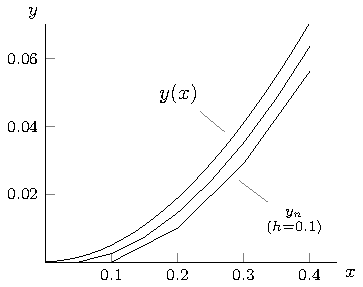
\includegraphics[]{figODEeuler}
\caption*{(ب)}
\end{subfigure}%
\caption{ترکیب یولر سے حاصل حل کا ریاضیاتی حل کے ساتھ موازنہ کیا گیا ہے۔}
\label{شکل_سادہ_اول_یولر_اصل_موازنہ}
\end{figure}

%====================
سوال \حوالہ{سوال_سادہ_اول_میدان_ڈھال_الف} تا سوال \حوالہ{سوال_سادہ_اول_میدان_ڈھال_ت} کے میدان ڈھال کو قلم و کاغذ سے کھینچتے ہوئے دیے ابتدائی نقطوں سے گزرتے منحنی حل حاصل کریں۔چند ڈھال میدان شکل \حوالہ{شکل_سوال_سادہ_اول_میدان_ڈھال_الف} اور شکل \حوالہ{شکل_سوال_سادہ_اول_میدان_ڈھال_پ} میں دیے گئے ہیں۔

%==========================

\حصہء{سوالات}
\ابتدا{سوال}\شناخت{سوال_سادہ_اول_میدان_ڈھال_الف}\quad \quad
$y'=1+y^2,\quad (\tfrac{\pi}{4},1)$
\انتہا{سوال}
%====================
\ابتدا{سوال}\شناخت{سوال_سادہ_اول_میدان_ڈھال_ب}\quad \quad
$y'=1-y^2,\quad (0,0)$
\انتہا{سوال}
%====================
\ابتدا{سوال}\شناخت{سوال_سادہ_اول_میدان_ڈھال_بب}\quad \quad
$yy'+8x=0,\quad (1,1)$
\انتہا{سوال}
%====================
\ابتدا{سوال}\شناخت{سوال_سادہ_اول_میدان_ڈھال_پ} \quad \quad
$y'=y-y^2,\quad (1,0)$
\انتہا{سوال}
%====================
\ابتدا{سوال} \شناخت{سوال_سادہ_اول_میدان_ڈھال_پپ}\quad \quad
$y'=x+\tfrac{1}{y},\quad (0,1)$
\انتہا{سوال}
%====================
\ابتدا{سوال} \شناخت{سوال_سادہ_اول_میدان_ڈھال_پپپ}\quad \quad
$y'=\sin^2 x,\quad (0,1)$
\انتہا{سوال}
%====================
\ابتدا{سوال}\شناخت{سوال_سادہ_اول_میدان_ڈھال_ت} \quad \quad
$y'=\sin^2 y,\quad (0,0)$
\انتہا{سوال}
%==================================
\begin{figure}
\centering
\begin{subfigure}{0.5\textwidth}
\centering
\begin{tikzpicture}
\def\length{sqrt(1+(1+y^2)^2)}
\begin{axis}[small, axis equal,axis lines*=middle,view={0}{90}, xlabel={$x$},ylabel={$y$},ylabel style={rotate=-90},ylabel style={at={(axis description cs:0.5,1.05)}},xmin=-4,xmax=4,ymin=-4,ymax=4,domain=-3.5:4, y domain=-3.5:4, samples=11,xlabel style={at={(axis description cs:1.05,0.5)}},xtick=\empty,ytick=\empty]
\addplot3 [gray, quiver={u={1/\length}, v={(1+y^2)/\length}, scale arrows=0.4,},-stealth] (x,y,0); %differential equation
\end{axis}
\end{tikzpicture}%
\caption*{(الف) \quad $y'=1+y^2$}
\end{subfigure}%
\begin{subfigure}{0.5\textwidth}
\centering
\begin{tikzpicture}
\def\length{sqrt(1+(1-y^2)^2)}
\begin{axis}[small, axis equal,axis lines*=middle,view={0}{90}, xlabel={$x$},ylabel={$y$},ylabel style={rotate=-90},ylabel style={at={(axis description cs:0.5,1.05)}},xmin=-4,xmax=4,ymin=-4,ymax=4,domain=-3.5:4, y domain=-3.5:4, samples=11,xlabel style={at={(axis description cs:1.05,0.5)}},xtick=\empty,ytick=\empty]
\addplot3 [gray, quiver={u={1/\length}, v={(1-y^2)/\length}, scale arrows=0.3},-stealth] (x,y,0); %differential equation
\end{axis}
\end{tikzpicture}%
\caption*{(ب) \quad $y'=1-y^2$}
\end{subfigure}%
\caption{سوال \حوالہ{سوال_سادہ_اول_میدان_ڈھال_الف} اور سوال \حوالہ{سوال_سادہ_اول_میدان_ڈھال_ب} کے ڈھال میدان۔}
\label{شکل_سوال_سادہ_اول_میدان_ڈھال_الف}
\end{figure}
%=============================
\begin{figure}
\centering
\begin{subfigure}{0.5\textwidth}
\centering
\begin{tikzpicture}
\def\length{sqrt(1+(-8*x/y)^2)}
\begin{axis}[small, axis equal,axis lines*=middle,view={0}{90}, xlabel={$x$},ylabel={$y$},ylabel style={rotate=-90},ylabel style={at={(axis description cs:0.5,1.05)}},xmin=-4,xmax=4,ymin=-4,ymax=4.5,domain=-3.8:4, y domain=-3.9:4, samples=11,xlabel style={at={(axis description cs:1.05,0.5)}},xtick=\empty,ytick=\empty]
\addplot3 [gray, quiver={u={1/\length}, v={(-8*x/y)/\length}, scale arrows=0.4,},-stealth] (x,y,0); %differential equation
\end{axis}
\end{tikzpicture}%
\caption*{(الف) \quad $y'=-\tfrac{8x}{y}$}
\end{subfigure}%
\begin{subfigure}{0.5\textwidth}
\centering
\begin{tikzpicture}
\def\length{sqrt(1+(y-y^2)^2)}
\begin{axis}[small, axis equal,axis lines*=middle,view={0}{90}, xlabel={$x$},ylabel={$y$},ylabel style={rotate=-90},ylabel style={at={(axis description cs:0.5,1.05)}},xmin=-4,xmax=4,ymin=-4,ymax=4,domain=-3.5:4, y domain=-3.5:4, samples=11,xlabel style={at={(axis description cs:1.05,0.5)}},xtick=\empty,ytick=\empty]
\addplot3 [gray, quiver={u={1/\length}, v={(y-y^2)/\length}, scale arrows=0.3},-stealth] (x,y,0); %differential equation
\end{axis}
\end{tikzpicture}%
\caption*{(ب) \quad $y'=y-y^2$}
\end{subfigure}%
\caption{سوال \حوالہ{سوال_سادہ_اول_میدان_ڈھال_بب} اور سوال \حوالہ{سوال_سادہ_اول_میدان_ڈھال_پ} کے ڈھال میدان۔}
\label{شکل_سوال_سادہ_اول_میدان_ڈھال_پ}
\end{figure}


%====================
ڈھال میدان کے استعمال سے تفرقی مساوات کے تمام حل سامنے آ جاتے ہیں۔بعض اوقات تفرقی مساوات کا تحلیلی حل حاصل کرنا ممکن ہی نہیں ہوتا۔درج ذیل دو سوالات میں ڈھال میدان سے اخذ حل اور دیے گئے تحلیلی حل کا موازنہ کرتے ہوئے ڈھال میدان سے حاصل حل کی درستگی کا اندازہ لگایا جا سکتا ہے۔

%=================
\ابتدا{سوال}\quad \quad
$y'=\sin x,\quad (\tfrac{\pi}{2},0),\quad y=-\cos x$
\انتہا{سوال}
%=====================
\ابتدا{سوال}\quad \quad
$y'=3x^2,\quad (0,0),\quad y=x^3$
\انتہا{سوال}
%=====================

%=============================
\ابتدا{سوال}
سوال \حوالہ{سوال_سادہ_اول_میدان_ڈھال_ب}، سوال \حوالہ{سوال_سادہ_اول_میدان_ڈھال_پ} اور سوال \حوالہ{سوال_سادہ_اول_میدان_ڈھال_ت} میں بے قابو متغیرہ \عددی{x} صریحاً  ظاہر نہیں کیا گیا ہے۔ایسی مساوات جن میں بے قابو متغیرہ کو صریحاً ظاہر نہ کیا جائے \اصطلاح{خود مختار}\فرہنگ{خود مختار!سادہ تفرقی مساوات}\فرہنگ{تفرقی!خود مختار}\حاشیہب{autonomous ordinary differential equations}\فرہنگ{autonomous!differential equation}\فرہنگ{differential!autonomous} سادہ تفرقی مساوات کہلاتے ہیں۔ خود مختار سادہ تفرقی مساوات کے  \اصطلاح{ہم میلان}\فرہنگ{ہم میلان}\حاشیہب{isoclines}\فرہنگ{isoclines} حل \عددی{f(x,y)=c} کی شکل و صورت کیا ہو گی؟

جواب:چونکہ \عددی{y'} کا دارومدار \عددی{x} پر نہیں ہے لہٰذا \عددی{x} تبدیل کرنے سے \عددی{y} کا میلان تبدیل نہیں ہو گا اور \عددی{f(x,y)=c} افقی محور کے متوازی خط ہوں گے۔ 
\انتہا{سوال}
%================

ایک جسم \عددی{y} محدد پر حرکت کرتی ہے۔لمحہ \عددی{t} پر نقطہ \عددی{y=0} سے جسم کا فاصلہ \عددی{y(t)} ہے۔سوالات \حوالہ{سوال_سادہ-اول_رفتار_الف} تا سوال \حوالہ{سوال_سادہ-اول_رفتار_پ} میں دئے شرائط کے مطابق جسم کی رفتار کی نمونہ کشی کریں۔ریاضی نمونے کی ڈھال میدان بناتے ہوئے  دیے گئے ابتدائی معلومات پر پورا اترتا منحنی خط کھینچیں۔ 

%=====================
\ابتدا{سوال}\شناخت{سوال_سادہ-اول_رفتار_الف}
جسم کی رفتار ضرب فاصلہ \عددی{y(t)} مستقل ہے جو \عددی{4} کے برابر ہے جبکہ \عددی{y(0)=4} کے برابر ہے۔

جوابات:\عددی{yy'=4}، \عددی{y=8t+16}
\انتہا{سوال}
%======================
\ابتدا{سوال}
رفتار ضرب وقت فاصلے کے برابر ہے۔لمحہ \عددی{t=1} پر فاصلہ \عددی{y(1)=2} ہے۔

جوابات:\عددی{y=y' t}، \عددی{y=2t}
\انتہا{سوال}
%=====================
\ابتدا{سوال}\شناخت{سوال_سادہ-اول_رفتار_پ}
مربع رفتار منفی مربع فاصلہ اکائی کے برابر ہے۔ابتدائی فاصلہ اکائی کے برابر ہے۔

جوابات:\عددی{y'=\sqrt{1+y^2}}، \عددی{\sinh^{-1}y=t+\sinh^{-1}1}
\انتہا{سوال}
%======================
\ابتدا{سوال}
ہوائی جہاز سے چھلانگ لگا کر زمین تک خیریت سے بذریعہ چھتری  اترا جا سکتا ہے۔گرتے ہوئے شخص پر آپس میں الٹ، دو عدد قوتیں عمل کرتی ہیں۔پہلی قوت زمینی کشش \عددی{F_1=mg} ہے جہاں \عددی{m} اس شخص کی کمیت اور \عددی{g=\SI{9.8}{\meter\per\second\squared}} ثقلی اسراع ہے۔یہ قوت انسان کو زمین کی طرف اسراع دیتی ہے۔دوسری قوت چھتری پر ہوا کے رگڑ سے پیدا قوت ہے جو اس شخص کی رفتار کو بڑھنے سے روکتی ہے۔چھتری پر ہوا کے رگڑ سے رفتار کے مربع کے متناسب قوت \عددی{F_2=cv^2} پیدا ہوتی ہے۔نیوٹن کی مساوات حرکت کہتی ہے کہ کسی بھی جسم پر قوت، اس جسم کی کمیت ضرب اسراع کے برابر ہوتی ہے۔چھتری سے زمین پر اترتے شخص کی نمونہ کشی کرتے ہوئے رفتار \عددی{v} کی سادہ تفرقی مساوات حاصل کریں۔کمیت کو \عددی{m=1} اور مستقل کو \عددی{c=1} لیتے ہوئے ڈھال میدان کھینچیں۔ تصور کریں کہ چھتری اس لمحہ کھلتی ہے جب شخص کی رفتار \عددی{v=\SI{15}{\meter\per\second}} ہو۔ایسی صورت میں منحنی حل حاصل کریں۔اس شخص کی اختتامی رفتار کیا ہو گی؟ کیا چھتری پر قوت رفتار کے راست متناسب ہونے کی صورت میں بھی چھتری کے ذریعہ ہوائی جہاز سے زمین تک خیریت سے چھلانگ لگائی جا سکتی ہے؟

جوابات:\عددی{mg-cv^2=m\tfrac{\dif v}{\dif t}}؛ گرنے کی رفتار اس قیمت پر رہتی ہے جہاں نیچے جانب قوت \عددی{mg} اور چھتری کی رکاوٹی اوپر جانب قوت \عددی{cv^2} برابر ہوں۔ایسی صورت میں گرتے شخص کی رفتار تبدیل نہیں ہوتی یعنی \عددی{y'=0} ہوتا ہے۔تفرقی مساوات میں \عددی{y'=0} پر کرتے اور \عددی{m=c=1} لیتے ہوئے اختتامی رفتار \عددی{v(t=\infty)=\SI{3.13}{\meter\per\second}} حاصل ہوتی ہے۔
\انتہا{سوال}
%=====================
\ابتدا{سوال}\شناخت{سوال_سادہ_اول_گول_دائرہ_ڈھال_میدان}
گول دائرے کی مساوات \عددی{x^2+y^2=r^2} ہے۔رداس \عددی{r} کو مستقل تصور کرتے ہوئے دائرے کی مساوات کا تفرق لیتے ہوئے  ڈھال میدان کی تفرقی مساوات حاصل کریں۔ڈھال میدان کھینچیں۔کیا آپ ڈھال میدان کو دیکھ کر کہہ سکتے ہیں کہ منحنی حل گول دائرے ہیں؟ اسی طرح \عددی{x^2+9y^2=c} کا تفرق لیتے ہوئے سادہ تفرقی مساوات حاصل کریں۔تفرقی مساوات کی ڈھال میدان کھینچیں۔ کیا ڈھال میدان کو دیکھ کر کہا جا سکتا ہے کہ منحنی حل بیضوی ہو گا؟

جوابات:\عددی{y'=-\tfrac{x}{y}}، \عددی{y'=-\tfrac{x}{9y}}
\begin{figure}
\centering
\begin{subfigure}{0.5\textwidth}
\centering
\begin{tikzpicture}
\def\length{sqrt(1+(x/y)^2)}
\begin{axis}[small, axis equal,axis lines*=middle,view={0}{90}, xlabel={$x$},ylabel={$y$},ylabel style={rotate=-90},ylabel style={at={(axis description cs:0.5,1.05)}},xmin=-4,xmax=4,ymin=-4,ymax=4,domain=-3.5:4, y domain=-3.5:4, samples=11,xlabel style={at={(axis description cs:1.05,0.5)}},xtick=\empty,ytick=\empty]
\addplot3 [gray, quiver={u={1/\length}, v={(-x/y)/\length}, scale arrows=0.3,},-stealth] (x,y,0); %differential equation
\end{axis}
\end{tikzpicture}%
\caption*{(الف) تفرقی مساوات \عددی{y'=-\tfrac{x}{y}} کی ڈھال میدان۔}
\end{subfigure}%
\begin{subfigure}{0.5\textwidth}
\centering
\begin{tikzpicture}
\def\length{sqrt(1+(x/(9*y))^2)}
\begin{axis}[small, axis equal,axis lines*=middle,view={0}{90}, xlabel={$x$},ylabel={$y$},ylabel style={rotate=-90},ylabel style={at={(axis description cs:0.5,1.05)}},xmin=-4,xmax=4,ymin=-4,ymax=4,domain=-3.5:4, y domain=-3.5:4, samples=11,xlabel style={at={(axis description cs:1.05,0.5)}},xtick=\empty,ytick=\empty]
\addplot3 [gray, quiver={u={1/\length}, v={(-x/(9*y))/\length}, scale arrows=0.3},-stealth] (x,y,0); %differential equation
\end{axis}
\end{tikzpicture}%
\caption*{(ب) تفرقی مساوات \عددی{y'=-\tfrac{x}{9y}} کی ڈھال میدان۔}
\end{subfigure}%
\caption{سوال \حوالہ{سوال_سادہ_اول_گول_دائرہ_ڈھال_میدان} کی ڈھال میدان۔}
\label{شکل_سوال_سادہ_اول_گول_دائرہ_ڈھال_میدان}
\end{figure}
\انتہا{سوال}
%===============================
سوال \حوالہ{سوال_سادہ_اول_یولر_الف} تا سوال \حوالہ{سوال_سادہ_اول_یولر_ت} کو ترکیب یولر سے حل کریں۔کل پانچ ہم فاصلہ نقطوں پر حل حاصل کریں۔ایک ہی کارتیسی محدد پر حاصل \عددی{y_1} تا \عددی{y_{5}} اور سوال میں دئے گئے حل \عددی{y(x)} کا خط کھینچیں۔
%=====================
\ابتدا{سوال}\شناخت{سوال_سادہ_اول_یولر_الف}
\begin{align*}
y'=-y,\quad y(0)=1,\quad h=0.1,\quad y(x)=e^{-x}
\end{align*}

جوابات: \عددی{y_1=0.9}، \عددی{y_2=0.81}، \عددی{y_3=0.729}، \عددی{y_4=0.6561}، \عددی{y_5=0.59049}
\انتہا{سوال}
%======================
\ابتدا{سوال}\شناخت{سوال_سادہ_اول_یولر_ب}
\begin{align*}
y'=-y,\quad y(0)=1,\quad h=0.01,\quad y(x)=e^{-x}
\end{align*}

جوابات: \عددی{y_1=0.99}، \عددی{y_2=0.9801}، \عددی{y_3=0.9703}، \عددی{y_4=0.9606}، \عددی{y_5=0.95099}
\انتہا{سوال}
%======================
\ابتدا{سوال}\شناخت{سوال_سادہ_اول_یولر_پ}
\begin{align*}
y'=1+3x^2,\quad y(1)=2,\quad h=0.1,\quad y(x)=x^3+x
\end{align*}

جوابات: \عددی{y_1=2.1}، \عددی{y_2=2.203}، \عددی{y_3=2.315}، \عددی{y_4=2.442}، \عددی{y_5=2.59}
\انتہا{سوال}
%======================
\ابتدا{سوال}\شناخت{سوال_سادہ_اول_یولر_ت}
\begin{align*}
y'=2xy,\quad y(0)=2,\quad h=0.01,\quad y(x)=e^{x^2-4}
\end{align*}

جوابات: \عددی{y_1=1.04}، \عددی{y_2=1.0818}، \عددی{y_3=1.1255}، \عددی{y_4=1.1712}، \عددی{y_5=1.2190}
\انتہا{سوال}
%======================

\حصہ{قابل علیحدگی سادہ تفرقی مساوات}
متعدد اہم سادہ تفرقی مساوات کو الجبرائی ترتیب دیتے ہوئے درج ذیل صورت میں لکھا جا سکتا ہے
\begin{align}\label{مساوات_سادہ_اول_قابل_علیحدگی-الف}
g(y)y'=f(x)
\end{align}
جس کو مزید یوں
\begin{align*}
g(y)\frac{\dif y}{\dif x} \dif x=f(x) \dif x
\end{align*}
یعنی
\begin{align*}
g(y)\dif y=f(x) \dif x
\end{align*}
لکھا جا سکتا ہے۔اس مساوات کے بائیں جانب صرف \عددی{y} متغیرہ اور دائیں جانب صرف \عددی{x} متغیرہ پایا جاتا ہے لہٰذا اس کا تکمل لیا جا سکتا ہے۔
\begin{align}\label{مساوات_سادہ_اول_قابل_علیحدگی-ب}
\int g(y)\dif y=\int f(x) \dif x+c
\end{align}
اگر \عددی{g(y)} اور \عددی{f(x)} قابل تکمل تفاعل ہوں تب مساوات \حوالہ{مساوات_سادہ_اول_قابل_علیحدگی-ب} سے مساوات \حوالہ{مساوات_سادہ_اول_قابل_علیحدگی-الف} کا حل حاصل کیا جا سکتا ہے۔اس ترکیب کو \اصطلاح{ترکیب علیحدگی متغیرات}\فرہنگ{ترکیب علیحدگی متغیرات}\فرہنگ{علیحدگی متغیرات!ترکیب}\حاشیہب{variable separation technique}\فرہنگ{variable separation} کہتے ہیں۔ مساوات \حوالہ{مساوات_سادہ_اول_قابل_علیحدگی-الف} کو \اصطلاح{قابل علیحدگی مساوات}\فرہنگ{قابل علیحدگی مساوات}\حاشیہب{separable equation}\فرہنگ{separable equation} کہتے ہیں۔

%=======================
\ابتدا{مثال}
مساوات \عددی{y'=1+y^2} قابل علیحدگی مساوات ہے چونکہ اس کو
\begin{align*}
\frac{\dif y}{1+y^2}=\dif x
\end{align*}
لکھا جا سکتا ہے جس کے دونوں اطراف کا تکمل لیتے ہوئے
\begin{align*}
\tan^{-1} y =x+c
\end{align*}
یعنی
\begin{align*}
y=\tan(x+c)
\end{align*}
حاصل ہوتا ہے جو تفرقی مساوات کا درکار حل ہے۔حاصل حل کو واپس تفرقی مساوات میں پر کرتے ہوئے تسلی کر لیں کہ یہی صحیح حل ہے۔
\انتہا{مثال}
%=================
\ابتدا{مثال}
قابل علیحدگی تفرقی مساوات \عددی{y'=xe^{-x} y^3} کو علیحدہ کرتے  ہوئے دونوں اطراف کا تکمل لے کر حل کرتے ہیں۔
\begin{align*}
y^{-3}\dif y&=xe^{-x} \dif x\\
\frac{y^{-2}}{-2}&=c-(x+1)e^{-x} \quad \quad \text{\RL{تکمل لیا گیا ہے}}\\
y^2&=\frac{1}{2(x+1)e^{-x}-2c}
\end{align*}
\انتہا{مثال}
%=================
\ابتدا{مثال}\شناخت{مثال_سادہ_اول_گھنٹی_الف}
درج ذیل ابتدائی قیمت تفرقی مساوات کو حل کریں۔
\begin{align*}
y'=-2xy,\quad y(0)=1
\end{align*} 

حل:مساوات کے متغیرات کو علیحدہ کرتے ہوئے تکمل کے ذریعہ حل کرتے ہیں۔
\begin{align*}
\int\frac{\dif y}{y}&=-\int 2x \dif x+c\\
\ln y&=-x^{2}+c_1\\
y&=ce^{-x^2}
\end{align*}
ابتدائی معلومات پر کرتے ہوئے \عددی{c=0} یعنی \عددی{c=e^{c_1}=1} ملتا ہے لہٰذا تفرقی مساوات کا مخصوص حل \عددی{y=e^{-x^2}} ہے جسے شکل \حوالہ{شکل_مثال_سادہ_اول_گھنٹی_الف} میں دکھایا گیا ہے اور جو \اصطلاح{گھنٹی نما}\فرہنگ{گھنٹی نما}\حاشیہب{bell shaped}\فرہنگ{bell shaped} ہے۔
\begin{figure}
\centering
\begin{tikzpicture}
\begin{axis}
\addplot[domain=-2:2,samples=60]{e^(-x^2)};
\end{axis}
\end{tikzpicture}
\caption{مثال \حوالہ{مثال_سادہ_اول_گھنٹی_الف} کا \اصطلاح{گھنٹی نما} حل۔}
\label{شکل_مثال_سادہ_اول_گھنٹی_الف}
\end{figure}
\انتہا{مثال}
%================
\ابتدا{مثال}\quad کاربن سے عمر دریافت کرنے کا طریقہ\\
طبعی معلومات: \اصطلاح{کائناتی شعاعیں}\فرہنگ{کائناتی شعاعیں}\حاشیہب{cosmic rays}\فرہنگ{cosmic rays} فضا میں تابکار کاربن \عددی{\ce{^{14}_{6}C}} بناتی ہیں۔یہ عمل زمین کی پیدائش سے اب تک ہوتا آ رہا ہے۔وقت کے ساتھ فضا میں \عددی{\ce{^{14}_{6}C}} اور \عددی{\ce{^{12}_{6}C}}\اصطلاح{ہم جا}\فرہنگ{ہم جا}\حاشیہب{isotopes}\فرہنگ{isotopes} کی تناسب ایک مخصوص قیمت حاصل کر چکی ہے۔کوئی بھی جاندار سانس لے کر یا خوراک کے ذریعہ فضا سے کاربن جذب  کرتا ہے۔یوں جب تک جانور زندہ رہے اس کی جسم میں دونوں ہم جا کاربن کی تناسب وہی ہو گی جو فضا میں ان کی تناسب ہے۔البتہ مرنے کے بعد جسم میں تابکار کاربن کی مقدار تابکاری تحلیل کی بنا گھٹتی ہے جبکہ غیر تابکار کاربن کی مقدار تبدیل نہیں ہوتی۔تابکار کاربن \عددی{\ce{^{14}_{6}C}} کی نصف زندگی \عددی{\num{5715}} سال ہے۔

اہرام مصر میں دفن مومیائی ہوئی فرعون کی لاش میں \عددی{\ce{^{14}_{6}C}} اور \عددی{\ce{^{12}_{6}C}} کا تناسب فضا کے تناسب کا \عددی{\SI{56.95}{\percent}} ہے۔لاش کی عمر دریافت کریں۔

حل:تابکار کاربن کی نصف زندگی سے تابکاری تحلیل کا مستقل \عددی{k} دریافت کرتے ہیں۔
\begin{align*}
y_0e^{-k(5715)}=\frac{y_0}{2}, \quad e^{-k(5715)}=\frac{1}{2}, \quad -k=\frac{\ln (\frac{1}{2})}{5715}, \quad k=0.0001213
\end{align*}
لاش میں ہم جا کاربن کی تناسب سے لاش کی عمر حاصل کرتے ہیں۔
\begin{align*}
e^{-0.0001213t}=0.5695,\quad -0.0001213t=\ln 0.5695,\quad t=4641
\end{align*}
یوں فرعون کی لاش \عددی{\num{4641}} سال پرانی ہے۔

\انتہا{مثال}
%=================
\ابتدا{مثال}\شناخت{مثال_سادہ_اول_مرکب}\quad مرکب بنانے کا عمل\\
کیمیائی صنعت میں  مرکب بنانے کا عمل عام ہے۔شکل \حوالہ{شکل_مثال_سادہ_اول_مرکب}-الف میں  پانی کی ٹینکی دکھائی گئی ہے جس میں ابتدائی طور پر \عددی{1000} لٹر پانی پایا جاتا ہے۔اس پانی میں کل \عددی{\SI{100}{\kilo\gram}} نمک ملایا گیا ہے۔پانی کو مسلسل ہلانے سے ٹینکی میں کثافت یکساں رکھی جاتی ہے۔ٹینکی میں \عددی{40} لٹر فی منٹ کی شرح سے نمکین پانی شامل کیا جاتا ہے۔اس پانی میں نمک کی مقدار \عددی{\SI{0.5}{\kilo\gram\per\litre}} ہے۔ٹینکی سے نمکین پانی کا انخلا \عددی{40} لٹر فی منٹ ہے۔ٹینکی میں نمک کی کل مقدار بالمقابل وقت دریافت کریں۔
\begin{figure}
\centering
\begin{subfigure}{0.5\textwidth}
\centering
\begin{tikzpicture}
   [ragged border/.style={ decoration={random steps, segment length=1mm, amplitude=0.5mm},
           decorate,}]
\pgfmathsetmacro{\x}{2}
\pgfmathsetmacro{\y}{2}

\fill[cyan!30]
        decorate[ragged border]{
        (-\x-\x/4,\y/2)--++(\x,0)
        }
        -- ++(0,-3/8*\y) --++ (\x/4,0) --++ (0,-\y/8) --++ (-\x-\x/4,0) --++(0,\y/2) -- cycle;
\fill[cyan!30](-\x-\x/4,3/4*\y)coordinate(inL)--++(-\x/4,0)--++(0,\y/8)--++(\x/4,0)coordinate(inU)--cycle;
\fill[cyan!30] (inL) to [out=0,in=120] ++(\x/4,-\y/3)--++(\x/16,0) to [out=120,in=0] (inU)--cycle;

\draw(0,0)--++(-\x-\x/4,0)--++(0,3/4*\y)--++(-\x/4,0)++(0,\y/8)--++(\x/4,0)--++(0,\y/4);
\draw(0,\y/8)--++(-\x/4,0)--++(0,\y);
\draw[cyan!30,-stealth,ultra thick] (\x/8,\y/16)--++(\x/4,0)node[right,color=black]{خروج};
\draw[cyan!30,stealth-,ultra thick] (-\x-\x/4-\x/4-\x/8,3/4*\y+\y/16)--++(-\x/4,0)node[pos=0.5,above,color=black]{دخول};
\end{tikzpicture}
\caption*{(الف)}
\end{subfigure}%
\begin{subfigure}{0.5\textwidth}
\centering
\begin{tikzpicture}
\begin{axis}[small,xlabel={$t\, (\text{\RL{منٹ}})$}, ylabel={$y(t)$},ylabel style={rotate=-90},ylabel style={at={(axis description cs:0,1.05)}}]
\addplot[domain=0:150]{500-400*e^(-0.04*x)};
\end{axis}
\end{tikzpicture}
\caption*{(ب)}
\end{subfigure}%
\caption{مثال \حوالہ{مثال_سادہ_اول_مرکب} میں مرکب بنانے کا عمل۔}
\label{شکل_مثال_سادہ_اول_مرکب}
\end{figure}

حل:چونکہ ٹینکی میں پانی شامل ہونے کی شرح اور پانی خارج ہونے کی شرح  برابر ہےیں لہٰذا ٹینکی میں پانی کی مقدار تبدیل نہیں ہوتی۔ٹینکی میں داخل ہونے والا ایک لٹر کا نمکین پانی \عددی{\SI{0.5}{\kilo\gram}} نمک ٹینکی میں شامل کرتا ہے۔یوں \عددی{40} لٹر فی منٹ سے داخل ہوتا پانی \عددی{40\times 0.5=\SI{20}{\kilo\gram\per\minute}} سے نمک شامل کرتا ہے۔کسی بھی لمحہ ٹینکی میں کل نمک کو \عددی{y} کلوگرام لکھتے ہوئے ٹینکی میں نمک کی کثافت کو \عددی{\tfrac{y}{1000}} کلوگرام فی لٹر لکھا جا سکتا ہے۔یوں خارج ہوتا پانی \عددی{40\times \tfrac{y}{1000}} کلوگرام فی منٹ نمک خارج کرتا ہے۔اس طرح نمک میں اضافے کی شرح \عددی{\tfrac{\dif y}{\dif t}} کو
\begin{align*}
y'&=\text{\RL{نمک شامل ہونے کی شرح}} -\text{\RL{نمک خارج ہونے کی شرح}}\quad \quad (\text{\RL{متوازن مساوات}})\\
&=20-\frac{40y}{1000}
\end{align*}
یعنی
\begin{align}
y'=0.04(500-y)
\end{align}
لکھا جا سکتا ہے جو قابل علیحدگی مساوات ہے لہٰذا اس میں متغیرات کو علیحدہ کرتے ہوئے تکمل کے ذریعہ حل کرتے ہیں۔
\begin{align*}
\frac{\dif y}{y-500}=-0.04\dif t, \quad \ln \abs{y-500}=-0.04t+c_1,\quad y=500+ce^{-0.04t}
\end{align*}
ٹینکی میں ابتدائی نمک کی کل مقدار \عددی{\SI{100}{\kilo\gram}} ہے۔اس معلومات کو درج بالا میں پر کرتے ہوئے مساوات کا مستقل \عددی{c} حاصل کرتے ہیں۔ 
\begin{align*}
100=500+c^{-0.04(0)},\quad c=-400
\end{align*}
یوں کسی بھی لمحے ٹینکی میں کل نمک کی مقدار درج ذیل ہے جس کو شکل-ب میں دکھایا گیا ہے۔
\begin{align*}
y(t)=500-400e^{-0.04t}
\end{align*}
شکل-ب کے مطابق ٹینکی میں آخرکار کل \عددی{\SI{500}{\kilo\gram}} نمک پایا جائے گا۔ یہی جواب بغیر کسی مساوات لکھے بھی حاصل کیا جا سکتا ہے۔اگر ٹینکی میں لگاتار نمکین پانی شامل کیا جائے اور اس سے پرانا پانی خارج کیا جائے تو آخرکار ٹینکی میں صرف نیا شامل کردہ پانی ہی پایا جائے گا۔چونکہ شامل کردہ پانی میں \عددی{0.5} کلوگرام فی لٹر نمک پایا جاتا ہے لہٰذا \عددی{1000} لٹر کی ٹینکی میں کل نمک \عددی{1000\times 0.5=\SI{500}{\kilo\gram}} ہو گا۔ 
\انتہا{مثال}
%=====================
\ابتدا{مثال}\شناخت{مثال_سادہ_اول_نیوٹن_قانون_ٹھنڈک} \quad نیوٹن قانون ٹھنڈک
گرمیوں میں ایک دفتر کا درجہ حرارت ایئر کنڈشنر کی مدد سے \عددی{\SI{21}{\degree\celsius}} پر رکھا جاتا ہے۔صبح سات بجے ایئر کنڈشنر چالو کیا جاتا ہے اور شام نو بجے اس کو بند کر دیا جاتا ہے۔ایک مخصوص دن کو شام نو بجے بیرونی درجہ حرارت \عددی{\SI{40}{\degree\celsius}} ہوتا ہے جبکہ صبح سات بجے بیرونی درجہ حرارت \عددی{\SI{30}{\degree\celsius}} تک گر چکا ہوتا ہے۔دفتر کے اندر رات دو بجے درجہ حرارت \عددی{\SI{26}{\degree\celsius}} ہوتا ہے۔صبح سات بجے دفتر کے اندر درجہ حرارت معلوم کریں۔

طبعی معلومات:تجربے سے معلوم کیا گیا ہے کہ حرارتی توانائی کو با آسانی منتقل کرتے جسم (مثلاً لوہا) کے درجہ حرارت میں تبدیلی کی شرح جسم اور اس کے گرد ماحول کے درجہ حرارت میں فرق کے راست تناسب  ہوتا ہے۔اس کو \اصطلاح{نیوٹن کا قانون ٹھنڈک}\فرہنگ{نیوٹن کا قانون ٹھنڈک}\حاشیہب{Newton's law of cooling}\فرہنگ{Newton!law of cooling} کہا جاتا ہے۔

حل:پہلا قدم: نمونہ کشی \\
دفتر کے اندرونی حرارت کو \عددی{T} سے ظاہر کرتے ہیں جبکہ بیرونی حرارت کو \عددی{T_b} سے ظاہر کرتے ہیں۔یوں نیوٹن کا قانون ٹھنڈک کی ریاضیاتی صورت درج ذیل ہو گی۔
\begin{align}
\frac{\dif T}{\dif t}=k(T-T_b)
\end{align}
دوسرا قدم:عمومی حل کی تلاش\\
اگرچہ دفتر کی دیواریں اور چھت حرارتی توانائی با آسانی منتقل نہیں کرتی ہم اسی کلیے کا سہارا لیتے ہوئے مسئلہ حل کریں گے۔یہاں بیرونی درجہ حرارت مستقل قیمت نہیں ہے لہٰذا درج بالا مساوات کو حل کرنا مشکل ہو گا۔انجنیئرنگ کے شعبے میں عموماً ایسی ہی مشکلات کا سامنہ کرنا ہوتا ہے۔ہمیں مسئلے کی سادہ صورت حل کرنا ہو گی۔اگر ہم تصور کریں کہ \عددی{T_b} مستقل قیمت ہے تب درج بالا مساوات کے متغیرات علیحدہ کئے جا سکتے ہیں۔چونکہ بیرونی درجہ حرارت \عددی{\SI{30}{\degree\celsius}} تا \عددی{\SI{40}{\degree\celsius}} رہا ہے لہٰذا ہم اس کی اوسط قیمت یعنی \عددی{\SI{35}{\degree\celsius}} کو بیرونی درجہ حرارت تصور کرتے ہوئے مسئلے کو حل کرتے ہیں۔مساوات کے متغیرات علیحدہ کرتے ہوئے تکمل لے کر اس کو حل کرتے ہیں۔
\begin{align*}
\frac{\dif T}{T-35}=k\dif t, \quad \ln\abs{T-35}=kt+c_1,\quad T-35=ce^{kt}
\end{align*}
تیسرا قدم:مخصوص حل کا حصول\\
اگر شام نو بجے کو لمحہ \عددی{t=0} لیا جائے اور وقت کو گھنٹوں میں ناپا جائے تب \عددی{T(0)=21} لکھا جائے گا جسے درج بالا میں پر کرتے ہوئے \عددی{c=-14} حاصل ہوتا ہے۔یوں مخصوص حل
\begin{align*}
T=35-14e^{kt}
\end{align*}
چوتھا قدم:مستقل \عددی{k} کا حصول\\
ہم جانتے ہیں کہ رات دو بجے  اندرونی درجہ حرارت  \عددی{\SI{26}{\degree\celsius}} ہے۔یاد رہے کہ شام نو بجے کو لمحہ \عددی{t=0} لیا گیا لہٰذا رات دو بجے \عددی{t=5} ہو گا۔
یوں \عددی{T(5)=26} لکھا جائے گا۔ان معلومات کو درج بالا مساوات میں پر کرتے ہوئے \عددی{k} حاصل کرتے ہوئے مکمل مساوات حاصل کرتے ہیں۔
\begin{align*}
26=35-14e^{5k},\quad k=-0.088, \quad T=35-14e^{-0.088t}
\end{align*}
آخری قدم:\\
صبح سات بجے اندرونی درجہ حرارت کا تخمینہ لگاتے ہیں یعنی \عددی{t=10} پر درجہ حرارت درکار ہے۔
\begin{align*}
T=35-14e^{-0.088(10)}=\SI{29.2}{\degree\celsius}
\end{align*} 
پوری رات میں اندرونی درجہ حرارت \عددی{\SI{8.2}{\degree\celsius}} بڑھ گیا ہے۔شکل \حوالہ{شکل_مثال_سادہ_اول_نیوٹن_قانون_ٹھنڈک} میں اندرونی درجہ حرارت بالمقابل وقت دکھایا گیا ہے۔
\begin{figure}
\centering
\begin{tikzpicture}
\begin{axis}[small,xlabel={$t\,\text{(گھنٹے)}$},ylabel={$T\, (\si{\degree\celsius})$},ytick={21,29.2},yticklabels={$21$,$29.2$},ylabel style={rotate=-90},ylabel style ={at={(axis description cs:0,1.05)}},xmin=0]
\addplot[domain=0:10]{35-14*e^(-0.088*x)};
\end{axis}
\end{tikzpicture}
\caption{مثال \حوالہ{مثال_سادہ_اول_نیوٹن_قانون_ٹھنڈک}: دفتر کا اندرونی درجہ حرارت بالمقابل وقت۔}
\label{شکل_مثال_سادہ_اول_نیوٹن_قانون_ٹھنڈک}
\end{figure}
\انتہا{مثال}
%=======================
\ابتدا{مثال} \quad پانی کا انخلا:\شناخت{مثال_سادہ_اول_ٹاری_سلی}
پانی کی ٹینکی کا رقبہ عمودی تراش \عددی{B=\SI{2}{\meter\squared}} ہے۔ٹینکی کی تہہ میں \عددی{r=\SI{0.5}{\centi\meter}} رداس کا گول سوراخ ہے جس سے پانی نکل رہا ہے۔ٹینکی میں پانی کی ابتدائی گہرائی \عددی{h_1=\SI{1.5}{\meter}} ہے۔ٹینکی کتنی دیر میں خالی ہو گی۔

طبعی معلومات:پانی کی سطح پر \عددی{m} کمیت پانی کی مخفی توانائی \عددی{mgh} ہے جہاں \عددی{g=\SI{9.8}{\meter\per\second\squared}} ثقلی اسراع اور \عددی{h} پانی کی گہرائی ہے۔سوراخ سے خارج ہوتے وقت یہ مخفی توانائی  حرکی توانائی \عددی{\tfrac{mv^2}{2}} میں تبدیل ہو جاتی ہے جہاں \عددی{v} رفتار کو ظاہر کرتی ہے۔مخفی توانائی اور حرکی توانائی کو برابر لکھتے ہوئے \عددی{v} کے لئے حل کرتے ہیں۔
\begin{align*}
\frac{mv^2}{2}=mgh,\quad v=\sqrt{2gh}
\end{align*}
شکل \حوالہ{شکل_مثال_سادہ_اول_ٹاری_سلی}-الف میں پانی کی دھار دکھائی گئی ہے۔جیسا کہ آپ دیکھ سکتے ہیں دھار سوراخ کے قریب سکڑتا ہے۔اگر سوراخ کا رقبہ \عددی{a} ہو تب سکڑے  ہوئے مقام پر دھار کا رقبہ عمودی تراش \عددی{0.6a} ہوتا ہے۔یوں سوراخ سے نکلا تمام پانی رقبہ \عددی{0.6a} سے گزرتا ہے اور یہی وہ مقام ہے جہاں پانی کا ہر ذرہ ایک ہی سمت میں رفتار \عددی{v} سے حرکت کرتا ہے۔

شکل \حوالہ{شکل_مثال_سادہ_اول_ٹاری_سلی}-ب میں ایک نالی دکھائی گئی ہے جس میں پانی کی رفتار \عددی{v} ہے۔ نالی کا رقبہ عمودی تراش \عددی{A} ہے۔لمحہ \عددی{t=0} پر  مقام \عددی{m} پر موجود پانی کا ذرہ وقت \عددی{\Delta t} میں \عددی{v\Delta} فاصلہ طے کرتے ہوئے مقام \عددی{n} تک پہنچ جائے گا۔یوں \عددی{\Delta t} کے دوران مقام \عددی{m} سے گزرا ہوا پانی نالی کو \عددی{m} تا \عددی{n} بھرے گا۔اس پانی کی مقدار \عددی{\Delta M=A v \Delta t} ہو گی۔اسی کلیے کو استعمال کرتے ہوئے شکل \حوالہ{شکل_مثال_سادہ_اول_ٹاری_سلی}-الف میں \عددی{\dif t} دورانیے میں کل \عددی{\dif M=0.6a v \dif t} پانی خارج ہو گا۔یوں پانی کی شرح انخلا درج ذیل ہو گی۔
 \begin{align}\label{مساوات_سادہ_اول_ٹورا_سلی}
\frac{\dif M}{\dif t}=0.6a\sqrt{2gh}
\end{align}
 
اس مساوات  کو \اصطلاح{قانون ٹاری سلی}\فرہنگ{قانون ٹاری سلی}\حاشیہب{Torricelli's law}\فرہنگ{Torricelli's law} کہتے ہیں۔
\begin{figure}
\centering
\begin{subfigure}{0.5\textwidth}
\centering
\begin{tikzpicture}
  [ragged border/.style={ decoration={random steps, segment length=1mm, amplitude=0.5mm},
           decorate,}]
\pgfmathsetmacro{\x}{2}
\pgfmathsetmacro{\y}{2}
\pgfmathsetmacro{\angA}{70}
\pgfmathsetmacro{\angB}{110}
%coloured water
\path(-\x/2-\x/16,0) to [out=-\angA,in=\angA]++(0,-\y/4)coordinate(kL);
\path(-\x/2+\x/16,0) to [out=-\angB,in=\angB]++(0,-\y/4)coordinate(kR);
\fill[cyan!30](-\x,\y-\y/8)--++(\x,0)-- ++(0,-\y+\y/8) --++ (-\x,0) --++ (0,\y-\y/8) -- cycle;
\fill[cyan!30] (-\x/2-\x/16,0) to [out=-\angA,in=\angA] (kL)--(kR) to [out=\angB,in=-\angB] ++(0,\y/4)--cycle;
\draw[stealth-stealth] (\x/8,0)--++(0,\y-\y/8)node[pos=0.5,fill=white]{$h$};
%drum
\draw(0,0)--++(0,\y);
\draw(0,0)--++(-\x/2+\x/16,0)++(-\x/8,0)--++(-\x/2+\x/16,0)--++(0,\y);
\draw[stealth-](-\x/2-\x/16,-\y/8)--++(-\x/4,0)--++(-\x/8,-\y/8)node[left]{$0.6a$};
\draw (-\x-\x/16,\y-\y/8)--++(-\x/4,0);
\draw (-\x-\x/16,\y-\y/8-\y/16)--++(-\x/4,0);
\draw[stealth-](-\x-\x/16-\x/8,\y-\y/8)--++(0,\y/4)node[above]{$\dif h$};
\draw[stealth-](-\x-\x/16-\x/8,\y-\y/8-\y/16)--++(0,-\y/4);
\end{tikzpicture}
\caption*{(الف)}
\end{subfigure}%
\begin{subfigure}{0.5\textwidth}
\centering
\begin{tikzpicture}
\pgfmathsetmacro{\x}{2}
\pgfmathsetmacro{\y}{2}
%water
\fill[cyan!10](0,0)--++(2*\x,0)--++(0,\y/8)--++(-2*\x,0)--cycle;
\fill[cyan!30](\x/2,0)--++(\x,0)--++(0,\y/8)--++(-\x,0)--cycle;
\draw[stealth-](-\x/8,\y/16)--++(-\x/4,0)node[pos=0.5,above]{$v$};
\draw[stealth-stealth](\x/2,-\y/8)--++(\x,0)node[pos=0.5,fill=white]{$v \Delta t$};
\draw(\x/2+\x/2,\y/16)--++(\x/2,\y/2)node[right]{$\Delta M=A v\Delta t$};
%pipe
\draw(0,\y/8)--++(2*\x,0);
\draw(0,0)--++(2*\x,0);
\draw[stealth-](\x/4,\y/8)--++(0,\y/4)--++(-\x/4,\y/4)node[above]{\RL{رقبہ عمودی تراش=$A$}};
\draw[dashed] (\x/2,-\y/4)node[below]{$m$}--++(0,\y/2);
\draw[dashed] (\x+\x/2,-\y/4)node[below]{$n$}--++(0,\y/2);

\end{tikzpicture}
\caption*{(ب)}
\end{subfigure}%
\caption{مثال \حوالہ{مثال_سادہ_اول_ٹاری_سلی}: پانی کا انخلا اور پانی کے دھار کا سکڑنا۔}
\label{شکل_مثال_سادہ_اول_ٹاری_سلی}
\end{figure}

حل:دورانیہ \عددی{\dif t} میں پانی کی انخلا کے بنا ٹینکی میں پانی کی گہرائی \عددی{\dif h} کم ہو گی جو \عددی{B \dif h} حجم کی کمی کو ظاہر کرتی ہے جہاں \عددی{B} ٹینکی کا رقبہ عمودی تراش ہے۔چونکہ پانی کے انخلا سے ٹینکی میں پانی کم ہوتا ہے لہٰذا درج ذیل لکھا جا سکتا ہے جو دیے گئے مسئلے کا تفرقی مساوات ہے۔
\begin{align}
0.6a\sqrt{2gh} \dif t=-B\dif h
\end{align}
متغیرات کو علیحدہ کرتے ہوئے حل کرتے ہیں۔
\begin{align*}
\frac{\dif h}{\sqrt{h}}=-\frac{0.6a \sqrt{2g}}{B} \dif t,\quad 2\sqrt{h}=-\frac{0.6a \sqrt{2g}}{B} t+c
\end{align*}
ابتدائی لمحہ \عددی{t=0} پر پانی کی گہرائی \عددی{h_1} ہے۔ان معلومات کو درج بالا میں پر کرتے ہوئے \عددی{c=2h_1} ملتا ہے لہٰذا تفرقی مساوات کا مخصوص حل درج ذیل ہے۔
\begin{align}\label{مساوات_سادہ_اول_ٹاری_سلی_ٹینکی_خالی}
 2\sqrt{h}=-\frac{0.6a \sqrt{2g}}{B} t+ 2\sqrt{h_1}
\end{align}
خالی ٹینکی سے مراد \عددی{h=0} ہے۔مخصوص حل میں \عددی{h=0} پر کرتے ہوئے ٹینکی خالی کرنے کے لئے درکار وقت حاصل کرتے ہیں۔
\begin{align*}
 2\sqrt{0}=-\frac{0.6a \sqrt{2g}}{B} t+ 2\sqrt{h_1}, \quad t=\frac{2\sqrt{h_1} B}{0.6a \sqrt{2g}}\\
t=\frac{2\sqrt{1.5} \times 2}{0.6\pi 0.005^2 \sqrt{2\times 9.8}}=\SI{23482}{\second} \approx \SI{6.52}{\hour}
\end{align*}
مساوات \حوالہ{مساوات_سادہ_اول_ٹاری_سلی_ٹینکی_خالی} کو شکل \حوالہ{شکل_مثال_سادہ_اول_ٹاری_سلی_خالی} میں دکھایا گیا ہے۔یاد رہے کہ \عددی{\SI{23482}{\second}} میں ٹینکی خالی ہو جاتی ہے لہٰذا ترسیم کو اتنے وقت کے لئے ہی کھینچا گیا ہے۔
\begin{figure}
\centering
\begin{tikzpicture}
\begin{axis}[axis lines*=middle,ylabel={$h$},ylabel style={rotate=-90},ylabel style={at={(axis description cs:0,1.05)}},xlabel={$t\, (\si{\second})$},scaled x ticks=false]
\pgfmathsetmacro{\ha}{1.5}
\pgfmathsetmacro{\B}{2}
\pgfmathsetmacro{\a}{pi*0.005^2}
%\pgfmathsetmacro{\k}{0.3*\a*sqrt(2*9.8)/\B}  %pgfmath calculate this value wrongly????
\pgfmathsetmacro{\k}{0.000052}
%
\addplot[domain=0:23480]({x},{(sqrt(\ha)-\k*x)^(2)});
\end{axis}
\end{tikzpicture}
\caption{مثال \حوالہ{مثال_سادہ_اول_ٹاری_سلی}: ٹینکی خالی ہونے کا عمل۔}
\label{شکل_مثال_سادہ_اول_ٹاری_سلی_خالی}
\end{figure}
\انتہا{مثال}
%======================

\جزوحصہء{علیحدگی متغیرات کی جامع ترکیب}
بعض اوقات نا قابل علیحدگی تفرقی مساوات کے متغیرات کو تبدیل کرتے ہوئے مساوات کو قابل علیحدگی بنایا جا سکتا ہے۔ اس ترکیب کو درج ذیل عملاً اہم قسم کی مساوات کے لئے سیکھتے ہیں جہاں \عددی{f(\tfrac{y}{x})} قابل تفرق تفاعل ہے مثلاً \عددی{\cos \tfrac{y}{x}}، \عددی{e^{(y/x)}} وغیرہ۔
\begin{align}
y'=f\left(\frac{y}{x}\right)
\end{align}  
مساوات کی صورت دیکھتے ہوئے \عددیء{\tfrac{y}{x}=u} لیتے ہیں۔یوں درج ذیل لکھا جا سکتا ہے
\begin{align}\label{مساوات_سادہ_اول_جامع_علیحدگی_الف}
y=ux,\quad y'=u+xu'
\end{align}
جنہیں \عددی{y'=f(\tfrac{y}{x})} میں پر کرتے ہوئے \عددی{u+xu'=f(u)} یعنی \عددی{xu'=f(u)-u} ملتا ہے۔اگر \عددی{f(u)-u \ne 0} ہو تب متغیرات علیحدہ کرتے ہوئے درج ذیل لکھا جا سکتا ہے۔
\begin{align} 
\frac{\dif u}{f(u)-u}=\frac{\dif x}{x}
\end{align}
%============
\ابتدا{مثال}
تفاعل \عددی{xy'-y=2x} کو حل کریں۔

حل:تفاعل کو \عددی{y'=\tfrac{y}{x}+2} لکھا جا سکتا ہے۔یوں \عددی{\tfrac{y}{x}=u} لیتے ہوئے  مساوات \حوالہ{مساوات_سادہ_اول_جامع_علیحدگی_الف} کے استعمال سے درج ذیل ملتا ہے۔
\begin{align*}
u+xu'=u+2, \quad \dif u=2\frac{\dif x}{x},\quad u=2\ln \abs{x}+c
\end{align*}
اس میں \عددی{u} کی جگہ واپس \عددی{\tfrac{y}{x}} پر کرتے ہوئے جواب حاصل ہوتا ہے۔
\begin{align*}
\frac{y}{x}=2\ln \abs{x}+c,\quad y=2x\ln \abs{x}+cx
\end{align*}
\انتہا{مثال}
%=========================

\حصہء{سوالات}
سوال \حوالہ{سوال_سادہ_اول_جامع_علیحدگی_الف} تا سوال \حوالہ{سوال_سادہ_اول_جامع_علیحدگی_ب} کے عمومی حل حاصل کریں۔حاصل حل کو واپس تفرقی مساوات میں پر کرتے ہوئے اس کی درستگی ثابت کریں۔

%=======================
\ابتدا{سوال}\شناخت{سوال_سادہ_اول_جامع_علیحدگی_الف}
$y^2y'+x^2=0$

جواب:\عددی{x^3+y^3=c}
\انتہا{سوال}
%=============================
\ابتدا{سوال}
$yy'+x=0$

جواب:\عددی{x^2+y^2=c}
\انتہا{سوال}
%=============================
\ابتدا{سوال}
$y'=\sec^2 y$

جواب:\عددی{y=\tan x+c}
\انتہا{سوال}
%=============================
\ابتدا{سوال}
$y'\cos x=y\sin x$

جواب:\عددی{y=c\sec x}
\انتہا{سوال}
%=============================
\ابتدا{سوال}
$y'=ye^{x-1}$

جواب:\عددی{\ln\abs{y}=e^{x-1}+c}
\انتہا{سوال}
%=============================
\ابتدا{سوال} 
\عددی{u=\tfrac{y}{x}} پر کرتے ہوئے \عددی{xy'=y+x^2\sin^2\frac{y}{x}} کو حل کریں۔

جواب:\عددی{\tfrac{\cos \tfrac{y}{x}-1}{\cos\tfrac{y}{x}+1}=ce^{2x}}
\انتہا{سوال}
%=============================
\ابتدا{سوال}
\عددی{y'=(2x+y)^2} کو حل کریں۔ایسا کرنے کی خاطر \عددی{u=2x+y} پر کرنا ہو گا۔

جواب:\عددی{y=-2x+\sqrt{2}\tan(\sqrt{2}x+c)}
\انتہا{سوال}
%=============================
\ابتدا{سوال} 
\عددی{u=\tfrac{y}{x}} پر کرتے ہوئے \عددی{xy'=y^2+y} کو حل کریں۔

جواب:\عددی{y=-\tfrac{x}{x+c}}
\انتہا{سوال}
%=============================
\ابتدا{سوال} \شناخت{سوال_سادہ_اول_جامع_علیحدگی_ب}
\عددی{u=\tfrac{y}{x}} پر کرتے ہوئے \عددی{xy'=x-y} کو حل کریں۔

جواب:\عددی{xy-x^2=c}
\انتہا{سوال}
%=============================

 ابتدائی قیمت سوال \حوالہ{سوال_سادہ_اول_ابتدائی_قیمت_الف} تا سوال \حوالہ{سوال_سادہ_اول_ابتدائی_قیمت_ب} کے مخصوص حل حاصل کریں۔

\ابتدا{سوال}\شناخت{سوال_سادہ_اول_ابتدائی_قیمت_الف}
\begin{align*}
xy'+y=0,\quad y(2)=8
\end{align*}

جواب:\عددی{y=\tfrac{16}{x}}
\انتہا{سوال}
%====================
\ابتدا{سوال}
\begin{align*}
y'=1+9y^2,\quad y(1)=0
\end{align*}

جواب:\عددی{y=\tfrac{1}{3}\tan[3(x-1)]}
\انتہا{سوال}
%======================
\ابتدا{سوال}
\begin{align*}
y' \cos^2 x=\sin^2 y, \quad y(0)=\frac{\pi}{4}
\end{align*}

جواب:\عددی{\tan y=\tfrac{1}{1-\tan x}}
\انتہا{سوال}
%==============================
\ابتدا{سوال}
\begin{align*}
y'=-4xy,\quad y(0)=5
\end{align*}

جواب:\عددیء{y=5e^{-2x^2}}
\انتہا{سوال}
%==================
\ابتدا{سوال}
\begin{align*}
y'=-\frac{2x}{y},\quad y(1)=2
\end{align*}

جواب:\عددی{2x^2+y^2=6}
\انتہا{سوال}
%==================
\ابتدا{سوال}
\begin{align*}
y'=(x+y-4)^2,\quad y(0)=5
\end{align*}

جواب:\عددی{x+y-4=\tan(x+\tfrac{\pi}{4})}
\انتہا{سوال}
%=================
\ابتدا{سوال}\شناخت{سوال_سادہ_اول_ابتدائی_قیمت_ب}
\begin{align*}
xy'=y+3x^4\cos^2 \frac{y}{x},\quad y(1)=0
\end{align*}

 جواب:اس میں \عددی{u=\tfrac{y}{x}} پر کرنے سے \عددی{\tan \tfrac{y}{x}=x^3-1} ملتا ہے۔
\انتہا{سوال}
%=================
\ابتدا{سوال}
کسی بھی لمحے پر جرثوموں کی تعداد بڑھنے کی شرح، اس لمحے موجود جرثوموں کی تعداد کے راست تناسب ہے۔اگر ان کی تعداد دو گھنٹوں میں دگنی ہو جائے تب چار گھنٹوں بعد ان کی تعداد کتنی ہو گی؟ چوبیس گھنٹوں بعد کتنی ہو گی؟  

جوابات:\عددی{y=y_0e^{0.34657t}}، \عددی{4y_0}، \عددی{4095y_0}
\انتہا{سوال}
%==================
\ابتدا{سوال}
جرثوموں کی شرح پیدائش موجودہ تعداد کے راست تناسب ہے۔ان کی شرح اموات بھی موجودہ تعداد کے راست تناسب ہے۔جرثوموں کی تعداد بڑھنے کی شرح کیا ہو گی؟ تعداد بالمقابل وقت کیا ہو گا؟ تعداد کہاں متوازن صورت اختیار کرے گی؟

جوابات:\عددی{\tfrac{\dif y}{\dif t}=\alpha y-\beta y} جہاں \عددی{\alpha} اور \عددی{\beta} بالترتیب پیدائشی اور امواتی راست تناسب کے مستقل ہیں۔ تعداد بالمقابل وقت کی مساوات \عددیء{y=y_0e^{(\alpha-\beta)t}} ہے۔اگر \عددی{\alpha > \beta} ہو تب تعداد بڑھتی رہے گی۔اس کے برعکس اگر \عددی{\alpha<\beta} ہو تب تعداد گھٹتی رہے گی حتٰی کہ جراثیم فنا ہو جائیں اور \عددی{\alpha=\beta} کی صورت میں تعداد وقت کے ساتھ تبدیل نہیں ہو گی۔ 
\انتہا{سوال}
%=================
\ابتدا{سوال}
عموماً جاندار مرنے کے بعد مکمل طور پر خاک میں مل جاتے ہیں اور ان کا نشان تک نہیں رہتا البتہ بعض اوقات حالات یوں ہوتے ہیں کہ ان کا جسم پتھر میں بدل جاتا ہے۔اس پتھریلی جسم میں موجود \عددی{\ce{^{14}_{6}C}} اور \عددی{\ce{^{12}_{6}C}} ہم جا کے تناسب  سے اس کی عمر کا تخمینہ لگایا جا سکتا ہے۔ دو ہزار سال پرانی پتھریلی مچھلی  میں کاربن کا تناسب، ابتدائی تناسب کے کتنا گنا ہو گا؟

جواب:\عددی{\SI{69.5}{\percent}}
\انتہا{سوال}
%================
\ابتدا{سوال}
طبیعیات میں \اصطلاح{بار بردار}\فرہنگ{بار بردار}\حاشیہب{charged}\فرہنگ{charged} ذروں کو \اصطلاح{مسرع خطی}\فرہنگ{مسرع خطی}\حاشیہب{linear accelerator}\فرہنگ{linear accelerator} کے ذریعہ اسراع دی جاتی ہے۔تصور کریں کہ مسرع خطی میں \عددی{\ce{^{4}_{2}He^{2+}}} داخل ہوتا ہے جس کی رفتار مستقل اسراع کے ساتھ \عددی{\SI{1.2}{\milli\second}} دورانیے میں \عددی{\SI{e3}{\meter\per\second}} سے بڑھا کر \عددی{\SI{1.6e4}{\meter\per\second}} کر دی جاتی ہے۔اسراع دریافت کریں۔اس دورانیے میں ذرہ کتنا فاصلہ طے کرتا ہے؟

جوابات:\عددی{\SI{1.25e7}{\meter\per\second\squared}}، \عددی{\SI{10.2}{\meter}} 
\انتہا{سوال}
%==================
\ابتدا{سوال}
ایک ٹینکی میں \عددیء{2000} لٹر پانی پایا جاتا ہے جس میں \عددی{\SI{150}{\kilo\gram}} نمک ملایا گیا ہے۔پانی کو مسلسل ہلانے سے کثافت یکساں رکھی جاتی ہے۔ٹینکی میں \عددی{10} لٹر فی منٹ تازہ پانی شامل کیا جاتا ہے۔ٹینکی سے پانی کا اخراج بھی \عددی{10} لٹر فی منٹ ہے۔ایک گھنٹہ بعد ٹینکی میں کل کتنا نمک پایا جائے گا؟

جوابات:\عددی{y=150e^{-\tfrac{t}{200}}}، \عددی{y=\SI{111}{\kilo\gram}}
\انتہا{سوال}
%===================
\ابتدا{سوال}
مریض کے زبان کے نیچے تھرمامیٹر رکھ کر اس کا درجہ حرارت ناپا جاتا ہے۔ کمرے اور مریض کے درجہ حرارت بالترتیب \عددی{\SI{25}{\degree\celsius}} اور \عددی{\SI{40}{\degree\celsius}} ہیں۔زبان کے نیچے رکھنے کے ایک منٹ بعد تھرمامیٹر کا پارہ \عددی{\SI{35}{\degree\celsius}} تک پہنچتا ہے۔ تھرمامیٹر کتنی دیر میں اصل درجہ حرارت کے قریب (مثلاً \عددی{\SI{39.9}{\degree\celsius}}) پہنچ پائے گا؟

جواب:\عددی{T=40-15e^{-1.204t}}، \عددی{t=\SI{4.16}{\minute}}
\انتہا{سوال}
%====================
\ابتدا{سوال}
\اصطلاح{سرطان}\فرہنگ{سرطان}\حاشیہب{cancer}\فرہنگ{cancer} کی مہلک بیماری میرے خاندان کے کئی افراد کی جان لے چکی ہے۔سن \عددی{1960} میں اینا کین لایرڈ\حاشیہب{Anna Kane Laird} سرطان کی رسولی کی افزائش کو ٹھیک طرح \اصطلاح{گامپرٹز تفاعل}\فرہنگ{گامپرٹز تفاعل}\فرہنگ{تفاعل!گامپرٹز}\فرہنگ{سرطان!گامپرٹز}\حاشیہب{Benjamin Gompertz}\فرہنگ{Benjamin Gompertz} سے ظاہر کرنے میں کامیاب ہوئے۔

سرطانی رسولی میں جسم کا نظام تباہ ہو جاتا ہے۔یوں رسولی میں موجود خلیوں تک آکسیجن اور خوراک کا پہنچنا ممکن نہیں رہتا۔رسولی کے اندرونی خلیے آکسیجن اور خوراک کی کمی کی بنا مر جاتے ہیں۔ان حقائق کی نمونہ کشی درج ذیل گامپرٹز تفرقی مساوات کرتی ہے جہاں \عددی{y} رسولی کی کمیت ہے۔
\begin{align}
y'=-Ay\ln y,\quad A>0
\end{align}

جواب:\عددی{\ln y=ce^{-At}}
\انتہا{سوال}
%===================
\ابتدا{سوال}
دھوپ میں کپڑے کی نمی خشک ہونی کی شرح کپڑے میں موجود نمی کے راست تناسب ہوتی ہے۔اگر پہلے پندرہ منٹ میں نصف پانی خشک ہو جائے تب  \عددی{\SI{99.9}{\percent}} پانی کتنی دیر میں خشک ہو گا؟ ہم  \عددی{\SI{99.9}{\percent}} خشک کو مکمل خشک تصور کر سکتے ہیں۔

جواب:\عددی{y=y_0e^{-0.0462t}}، \عددی{\SI{49.8}{\minute}}
\انتہا{سوال}
%==================
\ابتدا{سوال}\شناخت{سوال_سادہ_اول_رگڑ}\quad رگڑ \\
دو سطحوں کو آپس میں رگڑنے سے قوت رگڑ پیدا ہوتی ہے جو اس حرکت کو روکنے کی کوشش کرتی ہے۔خشک سطحوں پر پیدا قوت \عددی{\abs{F}=\mu \abs{N}} سے حاصل کی جا سکتی ہے جہاں \عددی{N} دونوں سطحوں پر عمودی قوت، \عددی{\mu} \اصطلاح{حرکی رگڑ کا مستقل}\فرہنگ{حرکی رگڑ کا مستقل}\فرہنگ{رگڑ!حرکی مستقل}\حاشیہب{coefficient of kinetic friction}\فرہنگ{friction!coefficient} اور \عددی{F} رگڑ سے پیدا قوت ہے۔
\begin{figure}
\centering
\begin{subfigure}{0.5\textwidth}
\centering
\begin{tikzpicture}
\pgfmathsetmacro{\len}{3}
\pgfmathsetmacro{\ang}{30}
\pgfmathsetmacro{\x}{\len*cos(\ang)}
\pgfmathsetmacro{\y}{\len*sin(\ang)}
\pgfmathsetmacro{\lenF}{1.5}
\pgfmathsetmacro{\xF}{\lenF*cos(\ang)}
\pgfmathsetmacro{\yF}{\lenF*sin(\ang)}
%
\draw (0,0)--++(\x,0)--++(0,\y)--(0,0);
\draw(\ang:1/2*\len)coordinate(kL) --++ (\ang:0.3)coordinate(A)--++(\ang+90:0.3)coordinate(B)--++(180+\ang:0.3)--++(\ang-90:0.3);
\draw([shift={(0:0.5)}]0,0) arc (0:\ang:0.5);
\draw(\ang/2:0.8)node{$\alpha$};
\draw[-latex] (kL)++(\ang+90:0.15)++(\ang:-0.1)--++(\ang:-0.5)node[above]{$v$};
\draw[dashed](\ang:\len)coordinate(C)--++(\ang+90:0.5)coordinate(D);
\draw[latex-]($(A)!0.5!(B)$)coordinate(E)--($(C)!(E)!(D)$)node[pos=0.5,above]{$s(t)$};
\draw[-latex](\ang:1/2*\len+0.15)++(\ang+90:0.15)node[circ]{}--++(0,-\lenF)node[pos=0.9,left]{$mg$}coordinate(Ftip);
\draw[latex-](Ftip)--++(\ang:\yF)coordinate(Htip);
\draw[latex-](Htip)--++(\ang+90:\xF)node[pos=0.5,right]{$N$};
\end{tikzpicture}
\caption*{(الف)}
\end{subfigure}%
\begin{subfigure}{0.5\textwidth}
\centering
\begin{tikzpicture}
\pgfmathsetmacro{\angA}{70}
\pgfmathsetmacro{\angB}{110}
\draw(0,0) circle (1.2cm);
\draw[fill=gray!40] ([shift={(\angA:1.2cm)}]0,0) arc (\angA:\angB:1.2cm) --++(\angB:0.3cm) arc (\angB:\angA:1.5cm) --++(\angA:-0.3cm);
\draw(0,0)--++(\angA:1.2cm);
\draw(0,0)--++(\angB:1.2cm);
\draw([shift={(\angA:0.5)}]0,0)  arc (\angA:\angB:0.5);
\draw(\angA/2+\angB/2:0.8)node{$\Delta \phi$};
\draw[-latex] (\angA:1.35cm)--++(\angA-90:1cm)node[right]{$F+\Delta F$};
\draw[-latex] (\angB:1.35cm)--++(\angB+90:1cm)node[left]{$F$};
\end{tikzpicture}
\caption*{(ب)}
\end{subfigure}%
\caption{سوال \حوالہ{سوال_سادہ_اول_رگڑ} اور سوال \حوالہ{سوال_سادہ_اول_رسی_رگڑ} کے اشکال۔}
\label{شکل_سوال_سادہ_اول_رگڑ}
\end{figure}

شکل \حوالہ{شکل_سوال_سادہ_اول_رگڑ}-الف میں \عددی{\alpha} زاویہ کی سطح پر \عددی{m} کمیت کا جسم دکھایا گیا ہے۔اس پر ثقلی قوت (وزن) \عددی{mg} عمل کرتا ہے۔اس قوت کو دو حصوں میں تقسیم کیا جا سکتا ہے۔پہلا حصہ \عددی{N} ہے جو سطح کے عمودی ہے۔دوسرا حصہ سطح کے متوازی ہے جو جسم کو اسراع دیتا ہے۔  کمیت \عددی{\SI{10}{\kilo\gram}}، ثقلی اسراع \عددی{g=\SI{9.8}{\meter\per\second\squared}}، رگڑ کا مستقل \عددی{\mu=0.25} اور زاویہ \عددی{\alpha=\SI{30}{\degree}} ہیں۔ ابتدائی رفتار صفر لیتے ہوئے رفتار \عددی{v} کی مساوات حاصل کریں۔یہ جسم کتنی دیر میں کل \عددی{\SI{15}{\meter}} فاصلہ طے کرے گا؟

جواب: \عددی{mg\sin \alpha-\mu mg\cos \alpha=m\tfrac{\dif v}{\dif t}}، \عددی{v=3.93t\,\si{\meter\per\second}}، \عددی{\SI{2.76}{\second}}
\انتہا{سوال}
%===================
\ابتدا{سوال}\شناخت{سوال_سادہ_اول_رسی_رگڑ}
شکل \حوالہ{شکل_سوال_سادہ_اول_رگڑ}-ب میں گول جسم کے گرد لپیٹی گئی رسی کا چھوٹا حصہ دکھایا گیا ہے۔تجربے سے معلوم ہوتا ہے کہ رسی کے چھوٹے حصے کے سروں پر قوت میں فرق زاویہ \عددی{\Delta \phi} اور قوت \عددی{F} کے راست متناسب ہوتا ہے۔رسی کو جسم کے گرد کتنی مرتبہ لپیٹنے سے ایک شخص \عددی{500} گنا زیادہ قوت کے گاڑی کو روک سکتا ہے؟

جوابات:\عددی{F=F_0e^{\phi}}، \عددی{\phi=\SI{6.21}{\radian}} یعنی \عددی{1.98} مرتبہ لپیٹنا ضروری ہے۔
\انتہا{سوال}
%====================
\ابتدا{سوال}
کارتیسی محدد کے محور پر گول دائرے \عددی{x^2+y^2=r^2} کا تفرقی مساوات \عددی{y_1'} حاصل کریں۔اسی طرح محور سے گزرتے ہوئے سیدھے خط کا تفرقی مساوات \عددی{y_2'} حاصل کریں۔دونوں تفرقی مساوات کا حاصل ضرب کیا ہو گا؟ اس حاصل ضرب سے آپ کیا اخذ کر سکتے ہیں؟

جواب:\عددی{y_1' y_2'=-1}؛ آپس میں عمودی ہیں۔
\انتہا{سوال}
%=====================
\ابتدا{سوال}
آپ کو ایسے تفاعل سے ضرور واسطہ پڑیگا جس کا تحلیلی تکمل حاصل کرنا ممکن نہیں ہو گا۔ایسا ایک تفاعل \عددی{e^{x^2}} ہے۔اس تفاعل کی \اصطلاح{مکلارن تسلسل}\فرہنگ{تسلسل!مکلارن}\فرہنگ{مکلارن تسلسل}\حاشیہب{Maclaurin's series}\فرہنگ{Maclaurin's series} کے پہلے چار ارکان کا تکمل حاصل کریں۔

جواب:\عددی{\int e^{x^2} \approx x+\tfrac{x^3}{3}+\tfrac{x^5}{10}+\tfrac{x^7}{36}+\cdots}
\انتہا{سوال}
%========================
\ابتدا{سوال}\شناخت{سوال_سادہ_اول_کرہ_ٹینکی}\quad قانون ٹاری سلی\\
کروی ٹینکی کا رداس \عددی{R} ہے۔اس کی تہہ میں چھوٹا سوراخ ہے جس کا رداس \عددی{r} ہے۔پوری طرح بھری ہوئی ٹینکی کتنی دیر میں خالی ہو گی۔اگر \عددی{R=\SI{1}{\meter}} اور \عددی{r=\SI{1}{\centi\meter}} ہو تب ٹینکی کتنی دیر میں خالی ہو گی؟

جواب:\عددی{0.6\pi r^2 \sqrt{2 g h } \dif t=-\pi[R^2+(h-R)^2]\dif h}،\\
 \عددی{t+c=-\tfrac{\sqrt{2gh}}{9gr^2}(30R^2-10hR+3h^2)}،\quad  \عددی{t_{\text{خالی}}=\tfrac{44R^2\sqrt{gR}}{9gr^2}}،\\
 دیے رداس کی ٹینکی \عددی{\SI{4.34}{\hour}} یعنی چار گھنٹے اور بیس منٹ میں خالی ہو گی۔
\انتہا{سوال}
%======================

\حصہ{قطعی سادہ تفرقی مساوات اور جزو تکمل}\شناخت{حصہ_سادہ_اول_جزو_تکمل}
ایسا تفاعل \عددی{u(x,y)} جس کے \اصطلاح{استمراری}\فرہنگ{استمراری}\حاشیہب{continuous partial differential}\فرہنگ{continuous!partial differential} (یعنی بلا جوڑ) جزوی تفرق پائے جاتے ہوں کا (مکمل) تفرق درج ذیل ہے۔
\begin{align}
\dif u=\frac{\partial u}{\partial x}\dif x+\frac{\partial u}{\partial y}\dif y
\end{align}
یوں اگر \عددی{u(x,y)=c} ہو تب \عددی{\dif u=0} ہو گا۔

مثال کے طور پر \عددی{u=xy+2(x-y)=7} کا تفرق
\begin{align*}
\dif u=(y+2)\dif x+(x-2)\dif y=0
\end{align*}
ہو گا جس سے درج ذیل تفرقی مساوات لکھی جا سکتی ہے۔
\begin{align*}
y'=\frac{\dif y}{\dif x}=-\frac{y+2}{x-2}
\end{align*}
الٹ چلتے ہوئے اس تفرقی مساوات کو ہم حل کر سکتے ہیں۔ اس مثال سے ایک ترکیب جنم دیتی ہے جس پر اب غور کرتے ہیں۔

درجہ اول سادہ تفرقی مساوات \عددی{y'=-\tfrac{M(x,y)}{N(x,y)}} یعنی
\begin{align}\label{مساوات_سادہ_اول_قطعی_الف}
M(x,y)\dif x+N(x,y)\dif y=0
\end{align}
کو اس صورت \اصطلاح{قطعی تفرقی مساوات}\فرہنگ{قطعی تفرقی مساوات}\فرہنگ{تفرقی مساوات!قطعی}\حاشیہب{exact differential equation}\فرہنگ{exact differential equation} کہتے ہیں جب اس کو درج ذیل لکھنا ممکن ہو جہاں \عددی{u(x,y)} کوئی تفاعل ہے۔
\begin{align}\label{مساوات_سادہ_اول_قطعی_ب}
\frac{\partial u}{\partial x}\dif x+\frac{\partial u}{\partial y}\dif y=0
\end{align}
یوں مساوات \حوالہ{مساوات_سادہ_اول_قطعی_الف} کو
\begin{align}
\dif u=0
\end{align}
لکھ کر تکمل لیتے ہوئے تفرقی مساوات کا عمومی \اصطلاح{خفی حل}\فرہنگ{خفی حل}\حاشیہب{implicit solution}\فرہنگ{implicit solution}
\begin{align}
u(x,y)=c
\end{align}
حاصل ہوتا ہے۔

مساوات \حوالہ{مساوات_سادہ_اول_قطعی_الف} اور مساوات \حوالہ{مساوات_سادہ_اول_قطعی_ب} کا موازنہ کرتے ہوئے ہم دیکھتے ہیں کہ مساوات \حوالہ{مساوات_سادہ_اول_قطعی_الف} تب قطعی تفرقی مساوات ہو گا جب ایسا \عددی{u(x,y)} پایا جاتا ہو کہ درج ذیل لکھنا ممکن ہو۔
\begin{align}
\frac{\partial u}{\partial x}&=M \label{مساوات_سادہ_اول_قطعی_شرط_الف}\\
\frac{\partial u}{\partial y}&=N\label{مساوات_سادہ_اول_قطعی_شرط_ب}
\end{align}
ان سے ہم تفرقی مساوات کے قطعی ہونے کا شرط اخذ کرتے ہیں۔

سطح \عددی{xy} پر ایسا خطہ جس کا سرحد بند منحنی ہو اور یہ منحنی اپنے آپ کو نہ کاٹتا ہو پر تصور کریں کہ  \عددی{M} اور \عددی{N} ایسے \اصطلاح{استمراری}\فرہنگ{استمراری تفاعل}\حاشیہب{continuous}\فرہنگ{continuous function} (یعنی \اصطلاح{بلا جوڑ}) تفاعل ہیں جن کے درجہ اول تفرق بھی اس خطے پر بے جوڑ ہیں۔تب مساوات \حوالہ{مساوات_سادہ_اول_قطعی_شرط_الف} کے تفرق درج ذیل ہوں گے۔
\begin{align*}
\frac{\partial M}{\partial y}&=\frac{\partial^2 u}{\partial y \partial x}\\
\frac{\partial N}{\partial x}&=\frac{\partial^2 u}{\partial x \partial y}
\end{align*}
استمراری شرط کی بنا  \عددی{\tfrac{\partial^2 u}{\partial y \partial x}} اور \عددی{\tfrac{\partial^2 u}{\partial x \partial y}} برابر ہیں لہٰذا درج ذیل لکھا جا سکتا ہے۔
\begin{align}\label{مساوات_سادہ_اول_قطعی_تفرقی_شرط}
\frac{\partial M}{\partial y}=\frac{\partial N}{\partial x}\quad \text{\RL{شرط قطعیت}}
\end{align}
مساوات \حوالہ{مساوات_سادہ_اول_قطعی_الف} کا قطعی تفرقی مساوات ہونے کے لئے مساوات \حوالہ{مساوات_سادہ_اول_قطعی_تفرقی_شرط} پر پورا اترنا \اصطلاح{لازمی}\فرہنگ{شرط!لازمی}\فرہنگ{لازمی شرط!قطعی تفرقی}\حاشیہب{necessary condition}\فرہنگ{necessary condition!exactness} اور  \اصطلاح{معقول}\فرہنگ{شرط!معقول}\فرہنگ{معقول شرط!قطعی تفرقی}\حاشیہب{sufficient condition}\فرہنگ{sufficient condition!exactness} شرط ہے۔

قطعی تفرقی مساوات کا حل حاصل کرتے ہیں۔مساوات \حوالہ{مساوات_سادہ_اول_قطعی_شرط_الف} کا \عددی{x} تکمل لیتے ہوئے درج ذیل لکھا جا سکتا ہے
\begin{align}\label{مساوات_سادہ_اول_قطعی_حل_الف}
u=\int M \dif x+k(y)
\end{align}
جہاں تکمل کا مستقل  از خود \عددی{y} کا تفاعل ہو سکتا ہے۔تکمل کا مستقل \عددی{k(y)} حاصل کرنے کی خاطر مساوات \حوالہ{مساوات_سادہ_اول_قطعی_حل_الف} کا جزوی تفرق  \عددی{\tfrac{\partial u}{\partial y}} لیتے ہوئے  مساوات \حوالہ{مساوات_سادہ_اول_قطعی_شرط_ب} کی مدد سے  \عددی{\tfrac{\dif k}{\dif y}} حاصل کرتے ہیں جس کا \عددی{y} تکمل لینے سے \عددی{k} حاصل ہو گا۔(مثال \حوالہ{مثال_سادہ_اول_قطعی_مساوات_الف} دیکھیں۔)

اسی طرح مساوات \حوالہ{مساوات_سادہ_اول_قطعی_شرط_ب}  کا \عددی{y} تکمل لیتے ہوئے درج ذیل لکھا جا سکتا ہے
\begin{align}\label{مساوات_سادہ_اول_قطعی_حل_ب}
u=\int N \dif y + m(x)
\end{align}
جہاں تکمل کا مستقل از خود \عددی{x} کا تفاعل ہو سکتا ہے۔تکمل کا مستقل \عددی{m(x)} حاصل کرنے کی خاطر مساوات \حوالہ{مساوات_سادہ_اول_قطعی_حل_ب} کا جزوی تفرق  \عددی{\tfrac{\partial u}{\partial x}} لیتے ہوئے  مساوات \حوالہ{مساوات_سادہ_اول_قطعی_شرط_الف} کی مدد سے \عددی{\tfrac{\dif m}{\dif x}=} حاصل کرتے ہیں جس کا \عددی{x} تکمل لینے سے \عددی{m} حاصل ہو گا۔

%==================
\ابتدا{مثال}\شناخت{مثال_سادہ_اول_قطعی_مساوات_الف}\quad قطعی تفرقی مساوات\\
درج ذیل کو حل کریں۔
\begin{align}\label{مساوات_سادہ_اول_مثال_قطعی_الف}
(1+2xy^3)\dif x+(2y+3x^2y^2)\dif y=0
\end{align}

حل:پہلے ثابت کرتے ہیں کہ یہ مساوات \اصطلاح{قطعی} ہے۔یہ مساوات \حوالہ{مساوات_سادہ_اول_قطعی_الف} کی طرح ہے جہاں
\begin{align*}
M&=1+2xy^3\\
N&=2y+3x^2y^2
\end{align*}
ہیں۔ \عددی{\tfrac{\partial M}{\partial y}} اور \عددی{\tfrac{\partial N}{\partial y}} لکھتے ہیں
\begin{align*}
\frac{\partial M}{\partial y}&=6xy^2\\
\frac{\partial N}{\partial x}&=6xy^2
\end{align*}
جو مساوات \حوالہ{مساوات_سادہ_اول_قطعی_تفرقی_شرط} پر پورا اترتے ہیں لہٰذا دی گئی مساوات قطعی تفرقی مساوات  ہے۔آئیں اب اس کو حل کرتے ہیں۔

مساوات \حوالہ{مساوات_سادہ_اول_قطعی_حل_الف} کو استعمال کرتے ہیں۔
\begin{align}\label{مساوات_سادہ_اول_قطعی_حل_پ}
u=\int (1+2xy^3)\dif x+k(y)=x+x^2y^3+k(y) 
\end{align}
اس کا \عددی{y} جزوی تفرق لیتے ہوئے مساوات \حوالہ{مساوات_سادہ_اول_قطعی_شرط_ب} کا استعمال کرتے
\begin{align*}
\frac{\partial u}{\partial y}=3x^2y^2+\frac{\dif k}{\dif y}=N=2y+3x^2y^2
\end{align*}
ہوئے \عددی{\tfrac{\dif k}{\dif y}} حاصل ہوتا ہے۔
\begin{align*}
\frac{\dif k}{\dif y}=2y
\end{align*}
اس کا \عددی{y} تکمل لیتے ہوئے \عددی{k} حاصل کرتے ہیں
\begin{align} \label{مساوات_سادہ_اول_قطعی_حل_ت}
k=\int 2y \dif y=y^2+c_1
\end{align}
جہاں \عددی{c_1} تکمل کا مستقل ہے۔چونکہ \عددی{k} صرف  \عددی{y} پر منحصر ہے لہٰذا \عددی{c_1} مستقل \عددی{x} پر منحصر نہیں ہو سکتا۔یوں مساوات \حوالہ{مساوات_سادہ_اول_قطعی_حل_پ} اور مساوات \حوالہ{مساوات_سادہ_اول_قطعی_حل_ت} سے قطعی تفرقی مساوات کا حاصل ہوتا ہے۔
\begin{align}\label{مساوات_سادہ_اول_قطعی_حل_ٹ}
u(x,y)=x+x^2y^3+y^2+c_1=0
\end{align}
آخر میں مساوات \حوالہ{مساوات_سادہ_اول_قطعی_حل_ٹ} کا تفرق لیتے ہوئے مساوات  \حوالہ{مساوات_سادہ_اول_مثال_قطعی_الف} حاصل کر کے حاصل حل کی درستگی ثابت کرتے ہیں۔
\begin{align*}
\dif u=\frac{\partial u}{\partial x}\dif x+\frac{\partial u}{\partial y}\dif y=(1+2xy^3)\dif x+(3x^2y^2+2y)\dif y
\end{align*}

\انتہا{مثال}
%===================
\ابتدا{مثال}\quad مخصوص حل\\
\عددی{N=2y+3x^2y^2} لیتے ہوئے مساوات \حوالہ{مساوات_سادہ_اول_مثال_قطعی_الف} کو حل کریں  جہاں \عددی{x=1} پر \عددی{y=2} ہے۔

حل:\عددی{\tfrac{\partial u}{\partial y}=N=2y+3x^2y^2} کا \عددی{y} تکمل
\begin{align}\label{مساوات_سادہ_اول_قطعی_دوسرا_متغیر}
u=\int (2y+3x^2y^2)\dif y+m(x)=y^2+x^2y^3+m(x)
\end{align} 
لے کر اس سے \عددی{\tfrac{\partial u}{\partial x}} لکھتے ہیں
\begin{align*}
\frac{\partial u}{\partial x}=2xy^3+\frac{\dif m}{\dif x}
\end{align*}
جو \عددی{M} کے برابر ہو گا
\begin{align*}
2xy^3+\frac{\dif m}{\dif x}=M=1+2xy^3
\end{align*}
جس سے
\begin{align*}
\frac{\dif m}{\dif x}=1, \quad m=x+c_2
\end{align*}
حاصل ہوتا ہے۔اس کو مساوات \حوالہ{مساوات_سادہ_اول_قطعی_دوسرا_متغیر} میں پر کرتے ہوئے تفرقی مساوات کا حل ملتا ہے۔
\begin{align*}
u=y^2+x^2y^3+x+c_2=0
\end{align*}
ابتدائی معلومات پر کرتے ہوئے
\begin{align*}
2^2+(1^2) (2^3)+1+c_2=0, \quad c=-13
\end{align*}
ملتا ہے جس سے مخصوص حل لکھتے ہیں۔
\begin{align*}
y^2+x^2y^3+x-13=0
\end{align*}
\انتہا{مثال}
%====================
\ابتدا{مثال}\شناخت{مثال_سادہ_اول_غیر_خطی}\quad غیر قطعی مساوات\\
مساوات \عددی{-y\dif x+x\dif y=0} میں \عددی{M=-y} اور \عددی{N=x} ہیں لہٰذا \عددی{\tfrac{\partial M}{\partial y}=-1} لیکن \عددی{\tfrac{\partial N}{\partial x}=1} ہے۔یوں دیا گیا مساوات \اصطلاح{غیر قطعی}\فرہنگ{غیر قطعی}\فرہنگ{قطعی!غیر}\حاشیہب{non exact}\فرہنگ{non exact} ہے۔یوں قطعی مساوات کی ترکیب قابل استعمال نہیں ہے۔آئیں قطعی مساوات کی ترکیب استعمال کرنے کی کوشش کریں۔مساوات \حوالہ{مساوات_سادہ_اول_قطعی_حل_الف} سے
\begin{align*}
u=\int -y \dif x+k(y)=-xy+k(y)
\end{align*}
ملتا ہے جس کا \عددیء{y} تفرق \عددی{\tfrac{\partial u}{\partial y}=-x+\tfrac{\dif k}{\dif y}} ہے جسے \عددی{N} یعنی \عددی{x} کے برابر پر کرنے سے 
\عددی{\tfrac{\dif k}{\dif y}=2x} ملتا ہے جس کا تکمل \عددی{k=2xy+c} ہے۔اب مستقل \عددی{k} صرف \عددی{y} پر منحصر ہو سکتا ہے جبکہ حاصل \عددی{k} اس شرط پر پورا نہیں اترتا لہٰذا اس کو رد کیا جاتا ہے۔یوں قطعی تفرقی مساوات کی ترکیب اس مثال میں دیے تفرقی مساوات کے حل کے لئے نا قابل استعمال ہے۔آپ \عددی{N} سے شروع کرتے ہوئے حل کرنے کی کوشش کر سکتے ہیں۔آپ اس راستے سے بھی حل حاصل نہیں کر پائیں گے۔
\انتہا{مثال}
%====================

\جزوحصہء{تخفیف بذریعہ جزو تکمل}
مثال \حوالہ{مثال_سادہ_اول_غیر_خطی} میں تفاعل \عددی{-y\dif x+x\dif y=0} غیر قطعی تھا البتہ اس کو \عددی{\tfrac{1}{x^2}} سے ضرب دینے
 سے \عددی{-\tfrac{y}{x^2}\dif x+\tfrac{1}{x}\dif y=0} حاصل ہوتا ہے جو قطعی مساوات  ہے۔آپ مساوات \حوالہ{مساوات_سادہ_اول_قطعی_تفرقی_شرط} استعمال کرتے ہوئے ثابت کر سکتے ہیں کہ یہ واقعی قطعی مساوات ہے۔حاصل قطعی مساوات کا حل حاصل کرتے ہیں۔
\begin{align}\label{مساوات_سادہ_اول_جزو_تکمل_الف}
-\tfrac{y}{x^2}\dif x+\tfrac{1}{x}\dif y=0, \quad \dif \left(\frac{y}{x}\right)=0,\quad \frac{y}{x}=c
\end{align}
اس ترکیب کو عمومی بناتے ہوئے ہم کہتے ہیں کہ غیر قطعی مساوات مثلاً
\begin{align}\label{مساوات_سادہ_اول_جزو_تکمل_حصول_الف}
P(x,y)\dif x+Q(x,y)\dif y=0
\end{align}
کو ایک مخصوص تفاعل \عددی{F} سے ضرب دینے سے قطعی مساوات
\begin{align}
FP\dif x+FQ\dif y=0
\end{align}
حاصل کی جا سکتی ہے۔تفاعل \عددی{F} \اصطلاح{جزو تکمل}\فرہنگ{جزو تکمل}\فرہنگ{تکمل!جزو}\حاشیہب{integrating factor}\فرہنگ{integrating factor} کہلاتا ہے اور یہ عموماً \عددی{x} اور \عددی{y} پر منحصر ہو گا۔حاصل قطعی مساوات کو حل کرنا ہم سیکھ چکے ہیں۔

%======================
\ابتدا{مثال}\quad جزو تکمل\\
مساوات \حوالہ{مساوات_سادہ_اول_جزو_تکمل_الف} میں جزو تکمل \عددی{\tfrac{1}{x^2}} تھا لہٰذا اس کا حل درج ذیل لکھا جا سکتا ہے۔
\begin{align*}
FP\dif x+FQ\dif y=\frac{-y\dif x+x\dif y}{x^2}=\dif \left(\frac{y}{x}\right)=0,\quad \frac{y}{x}=c
\end{align*}
مساوات \عددی{-y\dif x+x\dif y=0} کے  مزید جزو تکمل \عددی{\tfrac{1}{y^2}}، \عددی{\tfrac{1}{xy}} اور \عددی{\tfrac{1}{x^2+y^2}} ہیں جن سے درج ذیل لکھا جا سکتا ہے۔
\begin{align*}
\frac{-y\dif x+x\dif y}{y^2}&=\dif \left(\frac{x}{y}\right)=0, \quad \frac{x}{y}=c\\
\frac{-y\dif x+x\dif y}{xy}&=-\dif \left(\ln \frac{x}{y}\right),\quad \ln\frac{x}{y}=c_1,\quad \frac{x}{y}=x\\
\frac{-y\dif x+x\dif y}{x^2+y^2}&=\dif \left(\tan^{-1}\frac{x}{y}\right),\quad \tan^{-1}\frac{x}{y}=c_1,\quad \frac{x}{y}=c
\end{align*} 
\انتہا{مثال}
%=====================

\جزوحصہء{جزو تکمل کا حصول}
مساوات \عددی{M\dif x+N\dif y=0} کی قطعیت کا شرط \عددی{\tfrac{\partial M}{\partial y}=\tfrac{\partial N}{\partial x}}  مساوات \حوالہ{مساوات_سادہ_اول_قطعی_تفرقی_شرط}  ہے۔مساوات \عددی{FP\dif x+FQ\dif y=0} کے لئے اس شرط کو درج ذیل لکھا جائے گا
\begin{align}\label{مساوات_سادہ_اول_شرط_قطعیت_ب}
\frac{\partial}{\partial y} (FP)=\frac{\partial}{\partial x} (FQ)
\end{align}
جس کو زنجیری طریقہ تفرق سے درج ذیل لکھا جا سکتا ہے جہاں زیر نوشت تفرق کو ظاہر کرتی ہے (یعنی \عددی{F_y=\tfrac{\partial F}{\partial y}})۔
\begin{align}
F_yP+FP_y=F_x Q+FQ_x
\end{align}
یہ مساوات عموماً پیچیدہ ہو گا لہٰذا ہم اس پر مزید وقت ضائع نہیں کرتے۔ہم ایسے جزو تکمل تلاش کرنے کی کوشش کرتے ہیں جو صرف \عددی{x} یا صرف \عددی{y} پر منحصر ہو۔صرف \عددی{x} پر منحصر جزو تکمل کی صورت میں \عددی{F=F(x)} لکھا جائے گا اور \عددی{F_y=0} ہو گا جبکہ \عددی{F_x==F'=\tfrac{\dif F}{\dif x}} ہو گا۔یوں مساوات \حوالہ{مساوات_سادہ_اول_شرط_قطعیت_ب} درج ذیل صورت اختیار کر لیگا
\begin{align}
FP_y=F'Q+FQ_x
\end{align}
جسے \عددی{FQ} سے تقسیم کرتے ہوئے ترتیب دیتے ہیں۔
 \begin{align}\label{مساوات_سادہ_اول_جزو_تکمل_حصول_ب}
\frac{1}{F}\frac{\dif F}{\dif x}=R \quad \text{جہاں}\quad R=\frac{1}{Q}\left[ \frac{\partial P}{\partial y}-\frac{\partial Q}{\partial x}\right]
\end{align}
اس سے درج ذیل مسئلہ ثابت ہوتا ہے۔
%=======================

\ابتدا{مسئلہ}\شناخت{مسئلہ_سادہ_اول_جزو_تکمل_الف}
%\begin{theorem}\label{مسئلہ_سادہ_اول_جزو_تکمل_الف}
اگر مساوات \حوالہ{مساوات_سادہ_اول_جزو_تکمل_حصول_الف} سے مساوات \حوالہ{مساوات_سادہ_اول_جزو_تکمل_حصول_ب} میں حاصل کردہ  \عددی{R} صرف \عددی{x} پر منحصر ہو تب  مساوات \حوالہ{مساوات_سادہ_اول_جزو_تکمل_حصول_الف} کا جزو تکمل پایا جاتا ہے جسے مساوات \حوالہ{مساوات_سادہ_اول_جزو_تکمل_حصول_ب} کا تکمل لے کر حاصل کیا جا سکتا ہے۔
\begin{align}\label{مساوات_سادہ_اول_جزو_تکمل_مساوات_الف}
F(x)=e^{\int R(x) \dif x}
\end{align}
%\end{theorem}
\انتہا{مسئلہ}
%==============================

اسی طرح \عددی{F=F(y)} کی صورت میں مساوات \حوالہ{مساوات_سادہ_اول_جزو_تکمل_حصول_ب} کی جگہ درج ذیل ملتا ہے
 \begin{align}\label{مساوات_سادہ_اول_جزو_تکمل_حصول_پ}
\frac{1}{F}\frac{\dif F}{\dif y}=R \quad \text{جہاں}\quad R=\frac{1}{P}\left[ \frac{\partial Q}{\partial x}-\frac{\partial P}{\partial y}\right]
\end{align}
جس سے درج بالا مسئلے کی جوڑی ملتی ہے۔
%======================

\ابتدا{مسئلہ}\شناخت{مسئلہ_سادہ_اول_جزو_تکمل_ب}
%\begin{theorem}\label{مسئلہ_سادہ_اول_جزو_تکمل_ب}
اگر مساوات \حوالہ{مساوات_سادہ_اول_جزو_تکمل_حصول_الف} سے مساوات \حوالہ{مساوات_سادہ_اول_جزو_تکمل_حصول_پ} میں حاصل کردہ  \عددی{R} صرف \عددی{y} پر منحصر ہو تب  مساوات \حوالہ{مساوات_سادہ_اول_جزو_تکمل_حصول_الف} کا جزو تکمل پایا جاتا ہے جسے مساوات \حوالہ{مساوات_سادہ_اول_جزو_تکمل_حصول_پ} کا تکمل لے کر حاصل کیا جا سکتا ہے۔
\begin{align}\label{مساوات_سادہ_اول_جزو_تکمل__مساوات_ب}
F(y)=e^{\int R(y) \dif y}
\end{align}
%
%\end{theorem}
\انتہا{مسئلہ}
%==============================
\ابتدا{مثال}\شناخت{مثال_سادہ_اول_جزو_تکمل_حصول}\quad جزو تکمل\\
دیے مساوات کا جزو تکمل حاصل کرتے ہوئے اس کا عمومی حل حاصل کریں۔ابتدائی معلومات \عددی{y(0)=-2} سے مخصوص حل حاصل کریں۔
\begin{align}\label{مساوات_سادہ_اول_مثال_جزو_تکمل}
(e^{x+y}+ye^y)\dif x+(xe^y-1)\dif y=0
\end{align}

حل:پہلا قدم:\quad غیر قطعیت ثابت کرتے ہیں۔مساوات \حوالہ{مساوات_سادہ_اول_قطعی_تفرقی_شرط} پر درج ذیل پورا نہیں اترتا لہٰذا غیر قطعیت ثابت ہوتی ہے۔
\begin{align*}
\frac{\partial P}{\partial y}=e^{x+y}+e^y+ye^y,\quad \frac{\partial Q}{\partial x}=e^y, \quad \frac{\partial P}{\partial y}\ne  \frac{\partial Q}{\partial x}
\end{align*} 
دوسرا قدم:\quad جزو تکمل حاصل کرتے ہیں۔مساوات \حوالہ{مساوات_سادہ_اول_جزو_تکمل_حصول_ب} سے حاصل \عددی{R} کی قیمت \عددی{x} اور \عددی{y} دونوں پر منحصر ہے 
\begin{align*}
R=\frac{1}{Q}\left[ \frac{\partial P}{\partial y}-\frac{\partial Q}{\partial x}\right]=\frac{1}{xe^y-1}(e^{x+y}+e^y+ye^y-e^y)
\end{align*}
لہٰذا مسئلہ \حوالہ{مسئلہ_سادہ_اول_جزو_تکمل_الف} قابل استعمال نہیں ہے۔آئیں مسئلہ \حوالہ{مسئلہ_سادہ_اول_جزو_تکمل_ب} استعمال کر کے دیکھیں۔ \عددی{R} کو مساوات \حوالہ{مساوات_سادہ_اول_جزو_تکمل_حصول_پ} سے حاصل کرتے ہیں۔
\begin{align*}
R=\frac{1}{P}\left[ \frac{\partial Q}{\partial x}-\frac{\partial P}{\partial y}\right]=\frac{1}{e^{x+y}+ye^y}(e^y-e^{x+y}-e^{-y}-ye^y)=-1
\end{align*}
مساوات \حوالہ{مساوات_سادہ_اول_جزو_تکمل__مساوات_ب} سے جزو تکمل \عددی{F(y)=e^{-y}} حاصل ہوتا ہے۔مساوات \حوالہ{مساوات_سادہ_اول_مثال_جزو_تکمل} کو \عددی{F} سے ضرب دیتے ہوئے  درج ذیل قطعی مساوات ملتی ہے۔اس کو قطعیت کے لئے پرکھ کر دیکھیں۔آپ کو شرط قطعیت کے دونوں اطراف اکائی حاصل ہو گا۔
\begin{align*}
(e^{x}+y)\dif x+(x-e^{-y})\dif y=0
\end{align*}
مساوات \حوالہ{مساوات_سادہ_اول_قطعی_حل_الف} استعمال کرتے ہوئے حل حاصل کرتے ہیں۔
\begin{align*}
u=\int (e^{x}+y) \dif x+k(y)=e^x+xy+k(y)
\end{align*}
اس کا \عددی{y} تفرق لیتے ہوئے مساوات \حوالہ{مساوات_سادہ_اول_قطعی_شرط_ب} کے استعمال سے \عددی{\tfrac{\dif k}{\dif y}} حاصل کرتے ہیں جس کا تکمل \عددی{k} ہو گا۔
\begin{align*}
\frac{\partial u}{\partial y}=x+\frac{\dif k}{\dif y}=x-e^{-y}, \quad \frac{\dif k}{\dif y}=N=-e^{-y}, \quad k=e^{-y}+c_1
\end{align*}
یوں عمومی حل درج ذیل ہو گا جس کو شکل \حوالہ{شکل_مثال_سادہ_اول_جزو_تکمل_حصول} میں دکھایا گیا ہے۔
\begin{align}
u(x,y)=e^x+xy+e^{-y}=c
\end{align}
تیسرا قدم:مخصوص حل:\quad ابتدائی معلومات \عددی{y(0)=-2} کو عمومی حل میں پر کرتے ہوئے مستقل کی قیمت حاصل کرتے ہیں۔
\begin{align*}
e^0+(0)(-2)+e^{-(-2)}=c, \quad c=e^2
\end{align*}
یوں مخصوص حل \عددی{e^x+xy+e^{-y}=e^2=7.389} ہے۔

چھوتا قدم:عمومی حل اور مخصوص حل کو واپس دیے گئے مساوات میں پر کرتے ہوئے اس کی درستگی ثابت کریں۔
\begin{figure}
\centering
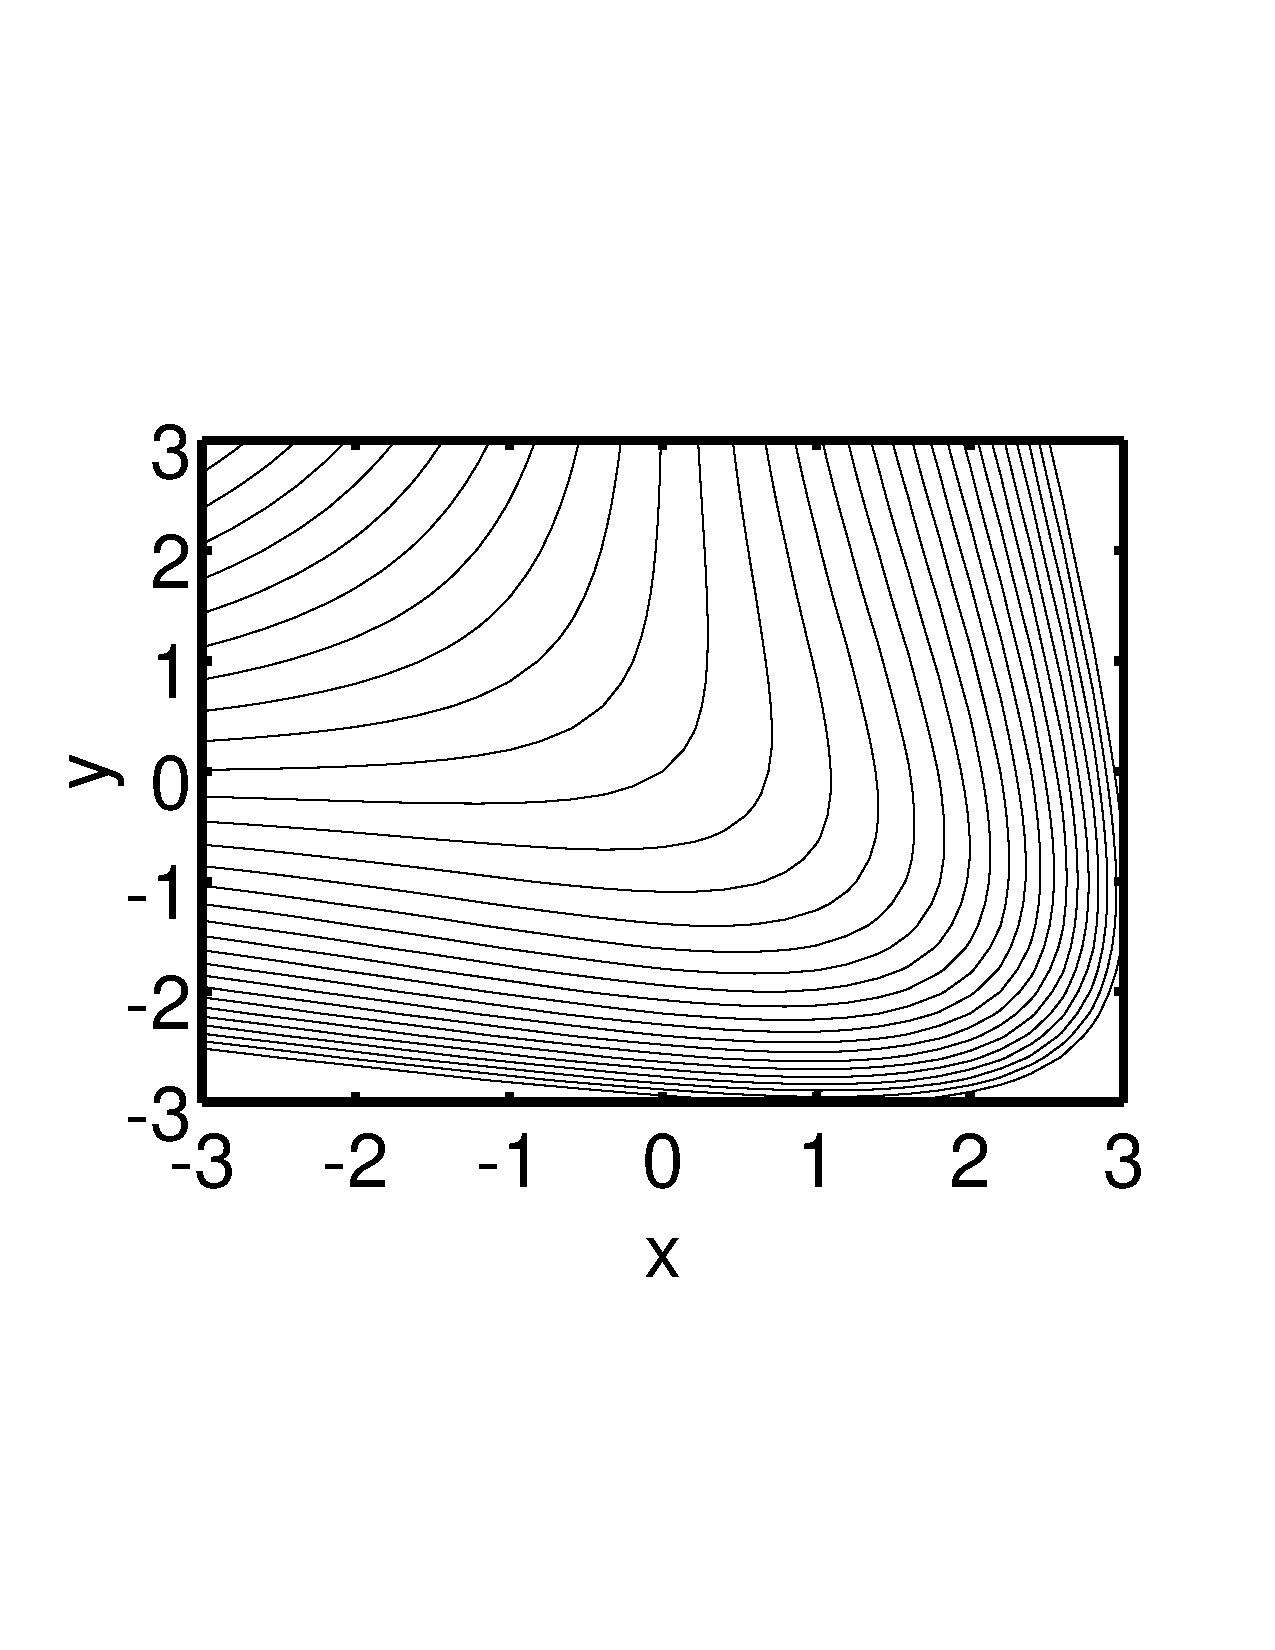
\includegraphics[height=3in]{integratingFactor}
\caption{مثال \حوالہ{مثال_سادہ_اول_جزو_تکمل_حصول}}
\label{شکل_مثال_سادہ_اول_جزو_تکمل_حصول}
\end{figure}
\انتہا{مثال}
%===========================

\حصہء{سوالات}
سوال \حوالہ{سوال_سادہ_اول_جزو_تکمل_الف} تا سوال \حوالہ{سوال_سادہ_اول_جزو_تکمل_ب} کو قطعیت کے لئے پرکھیں اور حل کریں۔غیر قطعی صورت میں دیا گیا جزو تکمل استعمال کریں یا اس کو بھی حاصل کریں۔جہاں ابتدائی معلومات دی گئی ہو، وہاں مخصوص حل حاصل کریں۔

\ابتدا{سوال}\شناخت{سوال_سادہ_اول_جزو_تکمل_الف}
\begin{align*}
2xy \dif x+x^2\dif y=0
\end{align*}
جواب:\عددی{y=\tfrac{c}{x^2}}
\انتہا{سوال} 
%===================
\ابتدا{سوال}
\begin{align*}
x^2\dif x+y\dif y=0
\end{align*}

جواب:\عددی{2x^3+3y^2=c}
\انتہا{سوال}
%============================
\ابتدا{سوال}
\begin{align*}
[\sin x+(x+y^3)\cos x]\dif x+3y^2\sin x \dif y=0
\end{align*}

جواب:\عددی{\sin x (x+y^3)}
\انتہا{سوال}
%===========================
\ابتدا{سوال}
\begin{align*}
(y+1)\dif x+(x+1)\dif y=0
\end{align*}

جواب:\عددی{x+xy+y=c}
\انتہا{سوال}
%=============================
\ابتدا{سوال}
\begin{align*}
(e^y+ye^x+y)\dif x+(xe^y+e^x+x)\dif y=0
\end{align*}

جواب:\عددی{xe^y+xy+ye^x}

\انتہا{سوال}
%=========================
\ابتدا{سوال}
\begin{align*}
\frac{y^2+4x}{x}\dif x+2y\dif y=0
\end{align*}

جواب:\عددی{F=x}، \عددی{u=(2x+y^2)x=c}
\انتہا{سوال}
%=============================
\ابتدا{سوال}
\begin{align*}
ye^x(2x+1+2y^2)\dif x+e^x(x+2y)\dif y=0
\end{align*}

جواب:\عددی{F=e^x}، \عددی{ye^{2x}(x+y)=c}
\انتہا{سوال}
%=============================
\ابتدا{سوال}
\begin{align*}
(2y^2+2xy+y)\dif x+(2y+x)\dif y=0
\end{align*}

جواب:\عددی{F=e^{2x}}، \عددی{e^{2x}(y^2+xy)=c}
\انتہا{سوال}
%=============================

\ابتدا{سوال}
\begin{align*}
y\dif x+(2xy-e^{-2y})\dif x=0, \quad y(1)=1
\end{align*}

جواب:\عددی{F=\tfrac{e^{2y}}{y}}، \عددی{xe^{2y}-\ln y=e^2}
\انتہا{سوال}
%==============
\ابتدا{سوال}
\begin{align*}
3(y+1)\dif x=2x\dif y,\quad y(1)=3,\quad F=\frac{y+1}{x^4}
\end{align*}

جواب:\عددی{y+1=4x^{\tfrac{3}{2}}}
\انتہا{سوال}
%=================
\ابتدا{سوال}
\begin{align*}
y\dif x+[y+\tan(x+y)]\dif y=0,\quad y(0)=\tfrac{\pi}{2},\quad F=\cos(x+y)
\end{align*}

جواب:\عددی{y\sin(x+y)=\tfrac{\pi}{2}}
\انتہا{سوال}
%=================
\ابتدا{سوال}\شناخت{سوال_سادہ_اول_جزو_تکمل_ب}
\begin{align*}
(a+1)y\dif x+(b+1)x \dif y=0,\quad y(1)=1, \quad F=x^ay^b
\end{align*}

جواب:\عددی{x^{a+1}y^{b+1}=0}
\انتہا{سوال}
%====================
\ابتدا{سوال}
جزو تکمل کو مزید بہتر سمجھنے کی خاطر  کسی بھی تفاعل مثلاً \عددی{u=e^{2x}(y^2+xy)=c} کے مکمل تفرق کو \عددی{M\dif +N\dif y=0} صورت میں لکھیں یعنی
 \عددی{e^{2x} (2y^2+2xy+y)\dif x+e^{2x}(2y+x)\dif y=0} جو قطعی مساوات ہے۔تفرقی مساوات کو \عددی{e^{2x}} سے تقسیم کرنے سے غیر قطعی مساوات 
\عددی{(2y^2+2xy+y)\dif x+(2y+x)\dif y=0} ملتا ہے۔۔اس غیر قطعی مساوات کو \عددی{e^{2x}} سے ضرب دیتے ہوئے قطعی بنایا جا سکتا ہے لہٰذا \عددی{e^{2x}} اس غیر قطعی مساوات کا جزو تکمل ہے۔
\انتہا{سوال}
%======================

\حصہ{خطی سادہ تفرقی مساوات۔ مساوات برنولی}
ایسے سادہ درجہ اول تفرقی مساوات جنہیں درج ذیل صورت میں لکھنا ممکن ہو \اصطلاح{خطی}\فرہنگ{خطی!سادہ تفرقی مساوات}\حاشیہب{linear}\فرہنگ{linear!ordinary differential equations} کہلاتے ہیں
\begin{align}\label{مساوات_سادہ_اول_خطی}
y'+p(x)y=r(x)
\end{align}
جبکہ ایسے مساوات جنہیں الجبرائی ترتیب دیتے ہوئے درج بالا صورت میں لکھنا ممکن نہ ہو \اصطلاح{غیر خطی} کہلاتے ہیں۔

خطی مساوات \حوالہ{مساوات_سادہ_اول_خطی} کی بنیادی خاصیت یہ ہے کہ اس میں تابع متغیرہ \عددی{y} اور تابع متغیرہ کا تفرق \عددی{y'} دونوں خطی ہیں جبکہ \عددی{p(x)} اور \عددی{r(x)} غیر تابع متغیرہ \عددی{x} کے \موٹا{کوئی} بھی تفاعل ہو سکتے ہیں۔اگر غیر تابع متغیرہ وقت ہو تب \عددی{x} کی جگہ \عددی{t} لکھا جاتا ہے۔

مساوات \حوالہ{مساوات_سادہ_اول_خطی} خطی مساوات کی معیاری صورت ہے جس کے پہلے رکن \عددی{y'} کا جزو ضربی اکائی ہے۔ایسی مساوات جس میں \عددی{y'} کی بجائے \عددی{f(x)y'} پایا جاتا ہو کو \عددی{f(x)} سے تقسیم کرتے ہوئے، اس کی معیاری صورت حاصل کی جا سکتی ہے۔ یوں خطی مساوات 
\عددی{(x+\sqrt{x})y'+y\sec x=e^x} کو \عددی{(x+\sqrt{x})} سے تقسیم کرتے ہوئے  اسے معیاری صورت \عددی{y'+\tfrac{\sec x}{x+\sqrt{x}}y=\tfrac{e^x}{x+\sqrt{x}}} میں لکھا جا سکتا ہے۔

دائیں ہاتھ \عددی{r(x)} \اصطلاح{قوت}\فرہنگ{قوت}\حاشیہب{force}\فرہنگ{force} کو ظاہر کر سکتی ہے جبکہ مساوات کا حل \عددی{y(x)} \اصطلاح{ہٹاو}\فرہنگ{ہٹاو}\حاشیہب{displacement}\فرہنگ{displacement} ہو سکتا ہے۔اسی طرح \عددی{r(x)} \اصطلاح{برقی دباو}\فرہنگ{برقی دباو}\حاشیہب{voltage}\فرہنگ{voltage} ہو سکتا ہے جبکہ \عددی{y(x)} \اصطلاح{برقی رو}\فرہنگ{برقی رو}\حاشیہب{current}\فرہنگ{current} ہو سکتی ہے۔ انجینئری میں \عددی{r(x)} کو عموماً \اصطلاح{درآیدہ}\فرہنگ{درآیدہ}\حاشیہب{input}\فرہنگ{input} یا \اصطلاح{جبری تفاعل}\فرہنگ{جبری تفاعل}\حاشیہب{forcing function}\فرہنگ{forcing function} کہتے ہیں جبکہ \عددی{y(x)} کو \اصطلاح{ماحصل}\فرہنگ{ماحصل}\حاشیہب{output}\فرہنگ{output} یا \اصطلاح{رد عمل}\فرہنگ{رد عمل}\حاشیہب{response}\فرہنگ{response} کہتے ہیں۔  
%================================

\جزوحصہء{متجانس خطی سادہ تفرقی مساوات}\شناخت{حصہ_سادہ_اول_متجانس_خطی}
ہم مساوات \حوالہ{مساوات_سادہ_اول_خطی} کو خطہ \عددی{a<x<b} میں حل کرنا چاہتے ہیں۔اس خطے کو \عددی{J} کہا جائے گا۔پہلے اس مساوات کی سادہ صورت حل کرتے ہیں جس میں \عددی{J} پر  تمام \عددی{x} کے لئے \عددی{r(x)} صفر کے برابر ہو۔ (اس کو بعض اوقات \عددی{r(x)\equiv 0} لکھا جاتا ہے۔) ایسی صورت میں مساوات \حوالہ{مساوات_سادہ_اول_خطی} درج ذیل صورت اختیار کرے گی 
\begin{align}\label{مساوات_سادہ_اول_ہم_جنسی_خطی_الف}
y'+p(x)y=0
\end{align}
جس کو \اصطلاح{متجانس}\فرہنگ{متجانس}\حاشیہب{homogeneous}\فرہنگ{homogeneous!linear ordinary differential equation} مساوات کہتے ہیں۔متغیرات علیحدہ کرتے ہوئے حل کرتے ہیں۔
\begin{align*}
\frac{\dif y}{y}=-\=p(x)\dif x,\quad \ln \abs{y}=-\int p(x) \dif x+c_1
\end{align*}
دونوں اطراف کا قوت نمائی لیتے ہوئے متجانس خطی مساوات \حوالہ{مساوات_سادہ_اول_ہم_جنسی_خطی_الف} کا حل حاصل ہوتا ہے۔
\begin{align}\label{مساوات_سادہ_اول_متجانس_حل_الف}
y(x)=ce^{-\int p(x)\dif x},\quad (c=\mp e^{c_1}\quad  \text{جب} \quad  y \lessgtr 0)
\end{align} 
یہاں \عددی{c=0} بھی چننا جا سکتا ہے جو \اصطلاح{غیر اہم حل}\فرہنگ{غیر اہم حل}\فرہنگ{حل!غیر اہم}\حاشیہب{trivial solution}\فرہنگ{trivial solution}\فرہنگ{solution!trivial} (یعنی \اصطلاح{صفر حل}) \عددی{y(x)=0} دیتا ہے۔
%====================

\جزوحصہء{غیر متجانس خطی سادہ تفرقی مساوات}
اب مساوات \حوالہ{مساوات_سادہ_اول_خطی} کو اس صورت میں حل کرتے ہیں جب \عددی{r(x) \not \equiv 0} ہو یعنی \عددی{J} پر کہیں کہیں یا پورے خطے پر  \عددی{r(x)} غیر صفر ہو۔ایسی صورت میں مساوات \حوالہ{مساوات_سادہ_اول_خطی} \اصطلاح{غیر متجانس}\فرہنگ{غیر متجانس}\حاشیہب{heterogeneous}\فرہنگ{heterogeneous} کہلاتا ہے۔غیر متجانس مساوات کی خوشگوار خاصیت یہ ہے کہ اس کا جزو تکمل \عددی{F(x)} صرف \عددی{x} پر منحصر ہوتا ہے لہٰذا اس کو مسئلہ \حوالہ{مسئلہ_سادہ_اول_جزو_تکمل_الف} کی مدد سے حاصل کیا جا سکتا ہے۔جزو تکمل کو حاصل کرتے ہیں۔غیر قطعی مساوات \حوالہ{مساوات_سادہ_اول_خطی} کو ترتیب دے کر \عددی{F} سے ضرب دیتے ہوئے قطعی مساوات حاصل کرتے ہیں
\begin{align*}
(py-r)\dif x+\dif y&=0,\quad F(py-r)\dif x+F\dif y=0
\end{align*}
جس سے مساوات \حوالہ{مساوات_سادہ_اول_قطعی_تفرقی_شرط} کی مدد سے درج ذیل ملتا ہے۔
\begin{align*}
\frac{\partial}{\partial y} [F(py-r)]=\frac{\partial F}{\partial x}\quad  \text{یعنی} \quad Fp=\frac{\partial F}{\partial x}
\end{align*}
متغیرات علیحدہ کرتے ہوئے تکمل لیتے ہوئے \عددی{F} حاصل کرتے ہیں۔
\begin{align*}
\frac{\dif F}{F}=p\dif x, \quad \ln \abs{F}=h(x)=\int p(x)\dif x \quad  \text{لہٰذا}\quad  F=e^h
\end{align*}
مساوات \حوالہ{مساوات_سادہ_اول_خطی} کو جزو تکمل \عددی{F} سے ضرب دیتے  اور \عددی{\tfrac{\dif h}{\dif x}=p} لکھتے ہوئے درج ذیل ملتا ہے
\begin{align*}
e^h y'+e^h h' y=e^h r \quad \text{یعنی}\quad  \left(e^h y\right)'=e^h r
\end{align*}
جس کا تکمل لیتے ہیں۔
\begin{align*}
e^h y=\int e^h r \dif x+c
\end{align*}
دونوں اطراف کو \عددی{e^h} سے تقسیم کرتے ہوئے غیر متجانس مساوات \حوالہ{مساوات_سادہ_اول_خطی} کا حل ملتا ہے۔
\begin{align}\label{مساوات_سادہ_اول_متجانس_خطی_حل_الف}
y=e^{-h}\left(\int e^h r \dif x+c\right), \quad h=\int p(x)\dif x
\end{align}
یوں مساوات \حوالہ{مساوات_سادہ_اول_خطی} کا حل درج بالا تکمل سے حاصل کیا جا سکتا ہے جو نسبتاً آسان ثابت ہوتا ہے۔اگر درج بالا تکمل بھی مشکل ثابت ہو تب تفرقی مساوات کا حل اعدادی ترکیب سے حاصل کیا جا سکتا ہے۔یہاں بتلاتا چلوں (سوال \حوالہ{سوال_سادہ_اول_برنولی_الف} دیکھیں) کہ \عددی{h} کے حصول میں تکمل کا مستقل کوئی کردار ادا نہیں کرتا لہٰذا اسے  صفر تصور کیا جاتا ہے۔

مساوات \حوالہ{مساوات_سادہ_اول_متجانس_خطی_حل_الف} کا تکمل درآیدہ \عددی{r(x)} پر منحصر ہے جبکہ ابتدائی معلومات تکمل کا مستقل \عددی{c} تعین کرتی ہیں۔اس مساوات کو درج ذیل لکھتے ہوئے 
\begin{align}\label{مساوات_سادہ_اول_متجانس_خطی_حل_ب}
y=e^{-h}\int e^h r \dif x+ce^{-h}
\end{align}
ہم دیکھتے ہیں کہ
\begin{align}
\text{کل ماحصل}=\text{درآیدہ سے پیدا رد عمل}+\text{ابتدائی معلومات سے پیدا رد عمل}
\end{align}

%=========================

\ابتدا{مثال}
ابتدائی قیمت تفرقی مساوات کو حل کریں۔
\begin{align*}
y'+y\cot x=2x\cosec x,\quad y\left(\frac{\pi}{2}\right)=0
\end{align*}

حل:یہاں \عددی{p=\cot x} اور \عددی{r=\cosec x} ہیں۔
\begin{align*}
h(x)=\int \cot x \dif x=\ln \abs{\sin x}
\end{align*}
یوں مساوات \حوالہ{مساوات_سادہ_اول_متجانس_خطی_حل_الف} میں
\begin{align*}
e^h=\sin x, \quad e^{-h}=\cosec x, \quad e^h r= (\sin x) (2x\cosec x)=2x
\end{align*}
ہیں لہٰذا عمومی حل
\begin{align*}
y=\cosec x \left(\int 2x\dif x +c\right)=\cosec x (x^2+c)
\end{align*}
ہو گا۔ابتدائی معلومات پر کرتے ہوئے  \عددی{c=-\tfrac{\pi^2}{4}} ملتا ہے لہٰذا مخصوص حل درج ذیل ہے
\begin{align*}
y=\cosec x \left(x^2-\frac{\pi^2}{4}\right)
\end{align*}
جس میں \عددی{x^2\cosec x} درآیدہ کا پیدا کردہ رد عمل ہے جبکہ \عددی{-\tfrac{\pi^2}{4}\cosec x} ابتدائی معلومات کا پیدا کردہ رد عمل ہے۔
\انتہا{مثال}
%==========================
\ابتدا{مثال}\شناخت{مثال_سادہ_اول_برقی_دور_الف} \quad برقی دور\\
شکل \حوالہ{شکل_مثال_سادہ_اول_برقی_دور_الف} میں \اصطلاح{مزاحمت}\فرہنگ{مزاحمت}\حاشیہب{resistance}\فرہنگ{resistance} \عددی{R} اور \اصطلاح{امالہ}\فرہنگ{امالہ}\حاشیہب{inductor}\فرہنگ{inductor} \عددی{L} سلسلہ وار جڑے ہیں۔اس دور کو \اصطلاح{سلسلہ وار}\فرہنگ{سلسلہ وار دور}\حاشیہب{series circuit}\فرہنگ{series circuit} \عددی{RL} دور کہتے ہیں۔لمحہ \عددی{t=0} پر \اصطلاح{برقی دباو}\فرہنگ{برقی دباو}\حاشیہب{electric voltage}\فرہنگ{voltage} \عددی{E} برقی دور پر لاگو کیا جاتا ہے جو دور میں \اصطلاح{برقی رو}\فرہنگ{برقی رو}\حاشیہب{electric current}\فرہنگ{current} \عددی{I(t)} کو جنم دیتا ہے۔ابتدائی رو صفر \عددیء{I(0)=0} کے برابر ہے۔

طبعی معلومات: مزاحمت کی اکائی \اصطلاح{اوہم}\فرہنگ{اوہم}\حاشیہب{Ohm}\فرہنگ{Ohm} \عددی{\si{\ohm}}  اور امالہ کی اکائی \اصطلاح{ہینری}\فرہنگ{ہینری}\حاشیہب{Henry}\فرہنگ{Henry} \عددی{\si{\henry}} ہے۔\اصطلاح{قانون اوہم}\فرہنگ{قانون اوہم}\حاشیہب{Ohm's law}\فرہنگ{Ohm's law} کے تحت مزاحمت \عددی{R} میں رو \عددی{I} اور دباو \عددی{v_R} کا تعلق \عددی{v_R=IR} ہے۔اسی طرح امالہ میں رو اور دباو \عددی{v_L} کا تعلق \عددی{v_L=L\tfrac{\dif I}{\dif t}} ہے۔ \اصطلاح{کرخوف قانون دباو}\فرہنگ{کرخوف!قانون دباو}\حاشیہب{Kirchoff's voltage law}\فرہنگ{Kirchoff's law!voltage} کے تحت ان برقی دباو کا مجموعہ درآیدہ دباو \عددی{E} کے برابر ہو گا۔ 
\begin{figure}
\centering
\begin{subfigure}{0.5\textwidth}
\centering
\begin{tikzpicture}[american voltages]
\draw(0,0) to [american voltage source,l={$\substack{\displaystyle E \hfill \\ \displaystyle \SI{50}{\volt}}$}]++(0,\yy) to [resistor,l={$\substack{\displaystyle R\hfill \\ \displaystyle \SI{100}{\ohm}}$},i={$I(t)$},v={$v_R$}]++(\xx,0) to [inductor,l_={$\substack{\displaystyle L \hfill \\ \displaystyle \SI{0.5}{\henry}}$},v^<={$v_L$}]++(0,-\yy) to [short]++(-\xx,0);
\end{tikzpicture}
\caption*{(الف)}
\end{subfigure}%
\begin{subfigure}{0.5\textwidth}
\centering
\begin{tikzpicture}
\begin{axis}[small,axis lines*=middle,xlabel={$t$},ylabel={$I(t)$},xtick={0.01,0.02,0.03},xticklabels={$0.01$,$0.02$,$0.03$},ytick={0,0.25,0.5,0.75},yticklabels={$0$,$0.25$,$\frac{E}{R}$,$0.75$},ylabel style={rotate=-90},ylabel style={at={(axis description cs:0,1.05)}},scaled x ticks=false,scaled y ticks=false]
\addplot[thick,domain=0:0.035]{50/100*(1-e^(-200*x))};
\addplot[domain=0:0.035]{0.5-0.25*e^(-200*x)};
\addplot[domain=0:0.035]{0.5+0.25*e^(-200*x)};
\end{axis}
\end{tikzpicture}
\caption*{(ب)}
\end{subfigure}%
\caption{مثال \حوالہ{مثال_سادہ_اول_برقی_دور_الف} کا سلسلہ وار برقی دور۔}
\label{شکل_مثال_سادہ_اول_برقی_دور_الف}
\end{figure}


حل:یہاں غیر تابع متغیرہ وقت \عددی{t} ہے جبکہ تابع متغیرہ رو \عددی{I(t)} ہے۔ کرخوف کے قانون کے تحت 
\begin{align*}
v_L+v_R=E, \quad L I'+RI=E, \quad I'+\frac{R}{L}I=\frac{E}{L}
\end{align*}
لکھا جائے گا جہاں آخری قدم پر \عددی{L} سے تقسیم کرتے ہوئے مساوات کو معیاری صورت میں لکھا گیا ہے۔اس کو مساوات \حوالہ{مساوات_سادہ_اول_متجانس_خطی_حل_الف} کی مدد سے حل کرتے ہیں جہاں \عددی{x} کی جگہ \عددی{t} اور \عددی{y} کی جگہ \عددی{I} استعمال ہو گا۔یہاں \عددی{p=\tfrac{R}{L}} اور \عددی{r=\tfrac{E}{L}} ہیں لہٰذا \عددی{h=\tfrac{R}{L}t} ہو گا اور عمومی حل
\begin{align*}
I=e^{-\frac{R}{L}t}\left(\int e^{\frac{R}{L}t}  \frac{E}{L} \dif x+c\right)
\end{align*}
لکھا جائے گا۔تکمل لیتے ہوئے درج ذیل ملتا ہے۔
\begin{align}\label{مساوات_سادہ_اول_برقی_مزاحمت_امالہ_سلسلہ_وار}
I=e^{-\frac{R}{L}t}\left(\frac{E}{L} \frac{e^{\frac{R}{L}}t}{\frac{R}{L}}+c\right)=\frac{E}{R}+ce^{-\frac{R}{L}t}
\end{align}
شکل \حوالہ{شکل_مثال_سادہ_اول_برقی_دور_الف}-الف میں پرزوں کی قیمتیں دی گئی ہیں جن سے \عددی{\tfrac{E}{R}=\tfrac{50}{100}=0.5} اور
 \عددی{\tfrac{R}{L}=\tfrac{100}{0.5}=200} ملتا ہے لہٰذا عمومی حل کو درج ذیل لکھا جا سکتا ہے۔
\begin{align}
I=0.5+ce^{-200t}
\end{align} 
مساوات \حوالہ{مساوات_سادہ_اول_برقی_مزاحمت_امالہ_سلسلہ_وار} میں ابتدائی معلومات پر کرتے ہوئے \عددی{c} کی قیمت حاصل ہوتی ہے۔ اس مساوات میں \عددی{ce^{-\tfrac{R}{L}t}} جزو \عددی{t \to \infty} پر صفر کے برابر ہو گا لہٰذا کافی دیر بعد رو پہلے جزو \عددی{\tfrac{E}{R}} کے برابر ہو گی جسے رو کی \اصطلاح{برقرار حال}\فرہنگ{برقرار حال}\حاشیہب{steady state}\فرہنگ{steady state} قیمت کہتے ہیں۔یہ ایک اہم نتیجہ ہے جس کے  تحت کافی دیر بعد رو کی قیمت کا دارومدار ابتدائی معلومات پر منحصر نہیں ہے۔رو کتنی جلدی برقرار حال قیمت اختیار کرتی ہے، اس کا دارومدار \عددی{\tfrac{R}{L}} کی قیمت پر ہے۔

مساوات \حوالہ{مساوات_سادہ_اول_برقی_مزاحمت_امالہ_سلسلہ_وار} میں ابتدائی معلومات \عددی{I(0)=0} پر کرتے  \عددی{0=0.5+ce^0} ہوئے \عددی{c=-0.5} ملتا ہے لہٰذا مخصوص حل درج ذیل ہو گا جس کو شکل \حوالہ{شکل_مثال_سادہ_اول_برقی_دور_الف}-ب میں موٹی لکیر سے دکھایا گیا ہے۔شکل میں ابتدائی قیمت \عددی{I(0)=0.25} اور \عددی{I(0)=0.75} سے حاصل مخصوص حل بھی دکھائے گئے ہیں۔
\begin{align}
I(t)=0.5(1-e^{-200t})
\end{align}
\انتہا{مثال}
%==========================
\ابتدا{مثال}\شناخت{مثال_سادہ_اول_غدود_درقیہ}\quad جسم میں ہارمونز کی مقدار\\
جسم میں موجود \اصطلاح{غدود}\فرہنگ{غدود}\حاشیہب{gland}\فرہنگ{gland} یعنی  \اصطلاح{گلٹی}\فرہنگ{گلٹی}، خون میں مختلف مرکبات\اصطلاح{(ہارمونز)}\فرہنگ{ہارمونز}\حاشیہب{hormones}\فرہنگ{hormones} خارج کرتے ہوئے مختلف نظام کو قابو کرتے ہیں۔تصور کریں کہ خون سے ایک مخصوص ہارمون مسلسل ہٹایا جاتا ہے۔ہٹانے کی شرح اس لمحے موجود ہارمون کی مقدار کے راست تناسب ہے۔ساتھ ہی ساتھ تصور کریں کہ روزانہ غدود اس ہارمون کو خون میں ایک مخصوص انداز سے خارج کرتی ہے۔خون میں موجود ہارمون کی نمونہ کشی کرتے ہوئے تفرقی مساوات کا عمومی حل حاصل کریں۔صبح چھ بجے خون میں ہارمون کی مقدار \عددی{y_0} لیتے ہوئے مخصوص حل حاصل کریں۔  

حل:پہلا قدم: نمونہ کشی:\quad چوبیس گھنٹوں میں خارج ہونے کے عمل کو \عددی{a+b\sin (\tfrac{2\pi t}{24})} سے ظاہر کرتے ہیں۔چونکہ خون میں ہارمون خارج ہونے سے خون میں ہارمون کی مقدار بڑھتی ہے لہٰذا \عددی{a\ge b} ہو گا۔یوں خارج کردہ ہارمون کی مقدار مثبت ہو گی۔کسی بھی لمحے خون میں ہارمون کی مقدار کی تبدیلی کی شرح، اس لمحے خون میں ہارمون کے داخل ہونے کی مقدار اور اس کی ہٹائی جانے والی مقدار میں فرق کے برابر ہو گا۔یوں مسئلے کا تفرقی مساوات درج ذیل ہو گا۔
\begin{align}
\frac{\dif y(t)}{\dif t}=a+b\sin\left(\frac{2\pi t}{24}\right)-k y(t) \quad \text{یعنی}\quad y'-ky=a+b\sin \omega t,\quad \omega =\frac{2\pi}{24}
\end{align}
دوسرا قدم: عمومی حل:\quad یہاں \عددی{p=k} ہے لہٰذا \عددی{h=\int k\dif t=kt} ہو گا۔اسی طرح \عددی{r=a+b\sin \omega t} ہے لہٰذا مساوات \حوالہ{مساوات_سادہ_اول_متجانس_خطی_حل_الف} سے عمومی حل درج ذیل ہو گا جس کو \اصطلاح{تکمل بالحصص}\فرہنگ{تکمل!بالحصص}\حاشیہب{integration by parts}\فرہنگ{integration!by parts} حل کیا گیا ہے
\begin{align*}
y&=e^{-kt}\int e^{kt} (a+b\sin \omega t) \dif t+ce^{-kt}\\
&=e{-kt}e^{kt}\left[\frac{a}{k}+\frac{b}{k^2+\omega^2}(k\cos \omega t+\omega \sin \omega t)\right]+ce^{-kt}\\
&=\frac{a}{k}+\frac{b}{k^2+\omega^2}(k\cos \omega t+\omega \sin \omega t)+ce^{-kt}
\end{align*}
عمومی حل کا آخری جزو وقت بڑھنے سے آخر کار صفر ہو جاتا ہے۔یوں \اصطلاح{برقرار حل}\فرہنگ{برقرار حل}\حاشیہب{steady state response}\فرہنگ{steady state response} بقایا اجزاء پر مشتمل ہے۔

آخر قدم:مخصوص حل:\quad صبح چھ بجے کو لمحہ \عددی{t=0} تصور کرتے ہوئے ابتدائی معلومات کو \عددی{y(0)=y_0} لکھا جا سکتا ہے۔ان قیمتوں کو عمومی حل میں پر کرتے ہوئے \عددی{c} کی قیمت حاصل کرتے ہیں۔
\begin{align*}
y_0 &=\frac{a}{k}+\frac{b}{k^2+\omega^2}(k\cos 0+\omega \sin 0)+ce^{0}, \quad \text{یعنی}\quad c=y_0-\frac{a}{k}-\frac{bk}{k^2+\omega^2}
\end{align*}
اس طرح مخصوص حل درج ذیل ہو گا۔مخصوص حل کو \عددی{a=1}، \عددی{b=1}، \عددی{k=0.04} اور \عددی{y_0=0} لیتے ہوئے  جسے شکل \حوالہ{شکل_مثال_سادہ_اول_غدود_درقیہ} میں دکھایا گیا ہے۔ شکل-ب میں \عددی{y_0=50} لیا گیا ہے۔آپ دیکھ سکتے ہیں کہ خون میں ہارمون کی مقدار بہت جلد ایک مخصوص اوسط قیمت پر پہنچ پاتی ہے۔
\begin{align*}
y=\frac{a}{k}+\frac{b}{k^2+\omega^2}(k\cos \omega t+\omega \sin \omega t)+(y_0-\frac{a}{k}-\frac{bk}{k^2+\omega^2})e^{-kt}
\end{align*}
%
\begin{figure}
\centering
\begin{subfigure}{0.5\textwidth}
\centering
\begin{tikzpicture}
\pgfmathsetmacro{\a}{2*pi/24}
\pgfmathsetmacro{\b}{2*pi/24}
\pgfmathsetmacro{\w}{2*pi/24}
\pgfmathsetmacro{\wa}{360/24}
\pgfmathsetmacro{\k}{0.04}
\pgfmathsetmacro{\ya}{0}
\begin{axis}[small,axis lines*=middle,ymin=0,ymax=55,xmin=0,xlabel={$t$},ylabel={$y(t)$},ylabel style={rotate=-90},ylabel style={at={(axis description cs:0,1.05)}}]
\addplot[domain=0:300,samples=400]{1/\k+(\k*cos(\wa*x)+\w*sin(\wa*x))/(\k^2+\w^2)+(\ya-1/\k-\k/(\k^2+\w^2))*e^(-\k*x)};
\end{axis}
\end{tikzpicture}
\caption*{(الف)}
\end{subfigure}%
\begin{subfigure}{0.5\textwidth}
\centering
\begin{tikzpicture}
\pgfmathsetmacro{\w}{2*pi/24}
\pgfmathsetmacro{\wa}{360/24}
\pgfmathsetmacro{\k}{0.04}
\pgfmathsetmacro{\ya}{50}
\begin{axis}[small,axis lines*=middle,ymin=0,ymax=55,xmin=0,xlabel={$t$},ylabel={$y(t)$},ylabel style={rotate=-90},ylabel style={at={(axis description cs:0,1.05)}}]
\addplot[domain=0:300,samples=400]{1/\k+(\k*cos(\wa*x)+\w*sin(\wa*x))/(\k^2+\w^2)+(\ya-1/\k-\k/(\k^2+\w^2))*e^(-\k*x)};
\end{axis}
\end{tikzpicture}
\caption*{(ب)}
\end{subfigure}%
\caption{مثال \حوالہ{مثال_سادہ_اول_غدود_درقیہ}: خون میں ہارمون کی مقدار بالمقابل وقت۔}
\label{شکل_مثال_سادہ_اول_غدود_درقیہ}
\end{figure}
\انتہا{مثال}
%=============================

\جزوحصہء{حصول خطی مساوات بذریعہ تخفیف۔ برنولی مساوات}
ایسے بہت سارے نظام ہیں جن کے غیر خطی سادہ تفرقی مساوات کو خطی بنایا جا سکتا ہے۔ان میں \اصطلاح{برنولی مساوات}\فرہنگ{برنولی مساوات}\حاشیہب{Bernoulli equation}\فرہنگ{Bernoulli!equation} 
\begin{align}\label{مساوات_سادہ_اول_برنولی_الف}
y'+p(x)y=g(x)y^a,\quad \text{\RL{$a$\, حقیقی عدد ہے}}
\end{align}
انتہائی اہم\حاشیہد{یعقوب برنولی (1654-1705): سوئزرلینڈ کے برنولی خاندان نے دنیا کو کئی اہم ریاضی داں دیے۔ یعقوب برنولی ان میں سر فہرست ہے۔انہوں نے علم الامکانیات میں بہت کام کیا۔قوت نمائی کا مستقل \عددی{e} بھی انہوں نے دریافت کیا۔} ہے۔برنولی مساوات \عددی{a=0} اور \عددی{a=1} کی صورت میں خطی ہے۔ اس کے علاوہ یہ غیر خطی ہے۔آئیں اس کو تبدیل کرتے ہوئے خطی مساوات حاصل کریں۔ہم
\begin{align*}
u(x)=[y(x)]^{1-a}
\end{align*}
کا تفرق لیتے ہوئے اس میں مساوات \حوالہ{مساوات_سادہ_اول_برنولی_الف} سے \عددی{y'} پر کرتے  ہوئے ترتیب دیتے ہیں۔
\begin{align*}
u'&=(1-a)y^{-a}y'\\
&=(1-a)y^{-a}(gy^a-py)\\
&=(1-a)g-(1-a)py^{1-a}\\
&=(1-a)g-(1-a)pu
\end{align*} 
یوں خطی سادہ تفرقی مساوات 
\begin{align}
u+(1-a)u'=(1-a)g
\end{align}
حاصل ہوتی ہے۔
%=============================

\ابتدا{مثال}\شناخت{مثال_سادہ_اول_نمو_آبادی}\quad ورہلسٹ مساوات برائے نمو آبادی
درج ذیل برنولی مساوات کو \اصطلاح{ورہلسٹ}\فرہنگ{ورہلسٹ}\حاشیہب{Pierre Francois Verhulst}\فرہنگ{Verhulst equation} مساوات کہتے ہیں جو \اصطلاح{نمو آبادی}\فرہنگ{نمو آبادی}\حاشیہب{population growth}\فرہنگ{population growth} کی تفرقی مساوات ہے۔اس کو حل کریں۔ (سوال \حوالہ{سوال_سادہ_اول_وبا} کو بھی دیکھیں۔)
\begin{align}\label{مساوات_سادہ_اول_ورہلسٹ_آبادی_نمو_الف}
y'=ay-by^2
\end{align}

حل:اس کو مساوات \حوالہ{مساوات_سادہ_اول_برنولی_الف} کی صورت \عددی{y'-ay=-by^2} میں لکھ کر \عددی{a=2} ملتا ہے۔یوں ہم \عددی{u=y^{1-a}=y^{-1}} کے تفرق میں مساوات \حوالہ{مساوات_سادہ_اول_ورہلسٹ_آبادی_نمو_الف} سے \عددی{y'}  پر کرتے ہیں
\begin{align*}
u'=-y^{-2}y'=-y^{-2}(ay-by^2)=-ay^{-1}+b=-ua+b
\end{align*}
جس سے خطی سادہ تفرقی مساوات
\begin{align*}
u'+au=b
\end{align*}
حاصل ہوتا ہے۔ مساوات \حوالہ{مساوات_سادہ_اول_متجانس_خطی_حل_الف} سے عمومی حل لکھتے ہیں۔
\begin{align*}
u=\frac{b}{a}+ce^{-at}
\end{align*}
چونکہ \عددی{u=y^{-1}} ہے لہٰذا اس سے درج ذیل ملتا ہے جس کو شکل \حوالہ{شکل_مثال_سادہ_اول_نمو_آبادی} میں دکھایا گیا ہے۔
\begin{align}\label{مساوات_سادہ_اول_نمو_آبادی}
y=\frac{1}{u}=\frac{1}{\frac{b}{a}+ce^{-at}}
\end{align}
مساوات \حوالہ{مساوات_سادہ_اول_ورہلسٹ_آبادی_نمو_الف} کو دیکھ کر \عددی{y(t)=0} حل بھی لکھا جا سکتا ہے۔ 
\begin{figure}
\centering
\begin{tikzpicture}
\pgfmathsetmacro{\a}{3}
\pgfmathsetmacro{\b}{1}
\pgfmathsetmacro{\ca}{100*\b/\a}
\pgfmathsetmacro{\caa}{1*\b/\a}
\pgfmathsetmacro{\cb}{-0.25*\b/\a}
\pgfmathsetmacro{\cc}{-0.375*\b/\a}
\pgfmathsetmacro{\cd}{-0.5*\b/\a}
\pgfmathsetmacro{\ce}{0*\b/\a}
\begin{axis}[small,axis lines*=middle,xmin=0,ymin=0,xlabel={$t$},ylabel={$y$},ylabel style={rotate=-90},ylabel style={at={(axis description cs:0,1.05)}},ytick={2,3,4,6},yticklabels={$2$,$\frac{a}{b}=3$,$4$,$6$}]
\addplot[domain=0:4,samples=50]{(\b/\a+\ca*e^(-\a*x))^(-1)};
\addplot[domain=0:4,samples=50]{(\b/\a+\caa*e^(-\a*x))^(-1)};
\addplot[domain=0:4,samples=50]{(\b/\a+\cb*e^(-\a*x))^(-1)};
\addplot[domain=0:4,samples=50]{(\b/\a+\cc*e^(-\a*x))^(-1)};
\addplot[domain=0:4,samples=50]{(\b/\a+\cd*e^(-\a*x))^(-1)};
\addplot[domain=0:4,samples=50]{(\b/\a+\ce*e^(-\a*x))^(-1)};
\end{axis}
\end{tikzpicture}
\caption{مثال \حوالہ{مثال_سادہ_اول_نمو_آبادی}: نمو آبادی کا خط۔}
\label{شکل_مثال_سادہ_اول_نمو_آبادی}
\end{figure}
\انتہا{مثال}
%===============================
\ابتدا{مثال}\شناخت{مثال_سادہ_درجہ_اول_متغیرات_بدلنے_کا_طریقہ}\quad مقدار معلوم بدلنے کا طریقہ\\
مساوات \حوالہ{مساوات_سادہ_اول_متجانس_خطی_حل_الف} کو ایک دلچسپ ترکیب سے حاصل کیا جا سکتا ہے جسے \اصطلاح{مقدار معلوم بدلنے کا طریقہ}\فرہنگ{مقدار معلوم!بدلنے کا طریقہ}\حاشیہب{variation of parameter}\فرہنگ{variation of parameter} کہتے ہیں۔متجانس مساوات \عددی{y'+p(x)y=0} کا  حل \عددی{y_1=ce^{-\int p(x) \dif x}} مساوات \حوالہ{مساوات_سادہ_اول_متجانس_حل_الف} دیتا ہے جس کو \عددی{y_1=ce^{-h}} لکھتے ہیں۔تصور کریں کہ غیر متجانس مساوات \عددی{y'+p(x)y=e(x)} کا حل \عددی{y_2=uy_1} لکھا جا سکتا ہے۔یوں \عددی{y_2'=u'y_1+uy_1'} ہو گا۔غیر متجانس مساوات میں \عددی{y_2} اور \عددی{y_2'} پر کرتے ہیں۔
\begin{align*}
u'y_1+uy_1'+p uy_1=r, \quad u'y_1+u(y_1'+py_1)=r,\quad u'y_1=r
\end{align*}
چونکہ \عددی{y_1}  متجانس مساوات کا حل ہے لہٰذا آخری قدم پر \عددی{y'+py=0} پر کرتے ہوئے \عددی{u'y_1=r} حاصل کیا گیا ہے۔اس سے \عددی{u} بذریعہ تکمل حاصل کرتے ہوئے \عددی{y_2} لکھتے ہیں جو مساوات \حوالہ{مساوات_سادہ_اول_متجانس_خطی_حل_الف} ہے۔  
\begin{align*}
u=\int \frac{r}{y_1}\dif x,\quad u=\int re^{h} \dif x+c, \quad \text{لہٰذا} \quad y_2=uy_1=e^{-h}\left[\int re^{h} \dif x+c\right]
\end{align*}


\انتہا{مثال}
%=============================
\جزوحصہء{نمو آبادی}
ورہلسٹ مساوات پودوں، جانوروں اور انسانی آبادی کی نمو کو ظاہر کرتی ہے۔اس مساوات  میں \عددی{b=0} پر کرنے سے  مالتھس مساوات \حوالہ{مساوات_سادہ_اول_مالتھس_الف} ملتی ہے جو آبادی کی بے روک نمو دیتی ہے۔ورہلسٹ مساوات میں جزو \عددی{-by^2}  آبادی بے قابو بڑھنے سے روکتی ہے۔ورہلسٹ مساوات کو \عددی{y'=ay(1-\tfrac{b}{a}y)} لکھ کر آپ دیکھ سکتے ہیں کہ \عددی{\tfrac{b}{a}y<1} کی صورت میں \عددی{y'>0} ہو گا اور آبادی  اس وقت تک مسلسل بڑھے گی جب تک بڑھے گی جبکہ  \عددی{\tfrac{b}{a}y<1} ہو، \عددی{\tfrac{b}{a}y>1} کی صورت میں \عددی{y'<0} ہو گا اور آبادی اس وقت تک مسلسل گھٹے گی جب تک \عددی{\tfrac{b}{a}y<1} ہو گا۔دونوں صورتوں میں عین \عددی{\tfrac{b}{a}y=1} یعنی \عددی{y=\tfrac{a}{b}} پر آبادی میں تبدیلی رک جائے گی۔شکل \حوالہ{شکل_مثال_سادہ_اول_نمو_آبادی} میں ایسا دکھایا گیا ہے۔

ورہلسٹ نمو آبادی کی مساوات میں غیر تابع متغیرہ \عددی{t} صریحاً نہیں پایا جاتا لہٰذا  یہ \اصطلاح{خود مختار}\فرہنگ{خود مختار!مساوات} مساوات ہے۔خود مختار مساوات
\begin{align}\label{مساوات_سادہ_اول_خود_مختار}
y'=f(y)
\end{align}
کے مستقل حل پائے جاتے ہیں جنہیں \اصطلاح{متوازن حل}\فرہنگ{متوازن حل}\حاشیہب{equilibrium solution}\فرہنگ{equilibrium!solution} یا \اصطلاح{متوازن نقطے}\فرہنگ{متوازن!نقطے}\حاشیہب{equilibrium points}\فرہنگ{equilibrium!points} کہا جاتا ہے۔خود مختار مساوات میں تفاعل \عددی{f(y)} کے صفر (f(y)=0) پر \عددی{y'=0} ہو گا جس کا حل \عددی{y=c} ہے جہاں \عددی{c} تکمل کا مستقل ہے۔تفاعل کے صفر کو مساوات \حوالہ{مساوات_سادہ_اول_خود_مختار} کے \اصطلاح{فاصل نقطے}\فرہنگ{فاصل نقطے}\حاشیہب{critical points}\فرہنگ{critical points} کہتے ہیں۔مساوات \حوالہ{مساوات_سادہ_اول_ورہلسٹ_آبادی_نمو_الف} کے فاصل نقطے \عددی{y=0} اور \عددی{y=\tfrac{a}{b}} ہیں۔یوں اس مساوات کے مستقل حل \عددی{y=0} اور \عددی{y=\tfrac{a}{b}} ہیں۔متوازن حل کو دو گروہ میں تقسیم کیا جاتا ہے جنہیں \اصطلاح{مستحکم}\فرہنگ{مستحکم}\حاشیہب{stable}\فرہنگ{stable} اور \اصطلاح{غیر مستحکم}\فرہنگ{غیر مستحکم}\حاشیہب{unstable}\فرہنگ{unstable} متوازن حل کہتے ہیں۔ ان کو شکل \حوالہ{شکل_مثال_سادہ_اول_نمو_آبادی} کی مدد سے سمجھا جا سکتا ہے جہاں \عددی{y=\tfrac{a}{b}=3} مستحکم حل ہے جبکہ \عددی{y=0} غیر مستحکم حل ہیں۔
%===================================



\حصہء{سوالات}
%================================
\ابتدا{سوال}\شناخت{سوال_سادہ_اول_برنولی_الف}
مساوات \حوالہ{مساوات_سادہ_اول_متجانس_خطی_حل_الف} میں \عددی{h} کے حصول میں تکمل کا مستقل صفر لیا جا سکتا ہے۔ایسا کیوں ممکن ہے؟
\انتہا{سوال}
%============================
\ابتدا{سوال}
ثابت کریں:
\begin{align*}
e^{\ln x}=x, \quad  e^{-\ln x}=\frac{1}{x}, \quad e^{-\ln \sec x}=\cos x
\end{align*}
\انتہا{سوال}
%==============================
سوال \حوالہ{سوال_سادہ_اول_برنولی_ب} تا سوال \حوالہ{سوال_سادہ_اول_برنولی_پ} کے عمومی حل تلاش کریں۔ابتدائی معلومات کی صورت میں مخصوص حل حاصل کریں اور اس کا خط کھینچیں۔

\ابتدا{سوال}\شناخت{سوال_سادہ_اول_برنولی_ب}
\begin{align*}
y'-y=2
\end{align*}

جواب:\عددی{y=ce^x-2}
\انتہا{سوال}
%==========================
\ابتدا{سوال}
\begin{align*}
y'-4y=2x
\end{align*}

جواب:\عددی{y=ce^{4x}-\tfrac{x}{2}-\tfrac{1}{8}}
\انتہا{سوال}
%===========================
\ابتدا{سوال}
\begin{align*}
y'+5y=e^{5x}, \quad y(0)=2
\end{align*}

جواب:\عددی{y=\tfrac{e^{5x}}{10}+\tfrac{19}{10}e^{-5x}}
\انتہا{سوال}
%===========================
\ابتدا{سوال}
\begin{align*}
y'+6y=4\sin 4x,\quad y\left(\frac{\pi}{8}\right)=6 
\end{align*}

جواب:\عددی{y=\tfrac{9}{13}\sin 4x-\tfrac{6}{13}\cos 4x+\tfrac{69}{13}e^{\tfrac{3\pi}{4}-6x}}
\انتہا{سوال}
%===========================
\ابتدا{سوال}
\begin{align*}
y'+2xy=2x,\quad y(0)=3
\end{align*}

جواب:\عددی{y=1+2e^{-x^2}}
\انتہا{سوال}
%===========================
\ابتدا{سوال}
\begin{align*}
xy'=2y+x^3e^x
\end{align*}

جواب:\عددی{y=x^2e^x+cx^2}
\انتہا{سوال}
%===========================
\ابتدا{سوال}
\begin{align*}
y'+y\tan x=\sin x
\end{align*}

جواب:\عددی{y=c \cos x-\cos x\ln \cos x}
\انتہا{سوال}
%===========================
\ابتدا{سوال}
\begin{align*}
y'+y\cos x=e^{-\sin x}
\end{align*}

جواب:\عددی{y=xe^{-\sin x}+ce^{-\sin x}}
\انتہا{سوال}
%===========================
\ابتدا{سوال}
\begin{align*}
\cos x y'+(4y-2)\sec x=0
\end{align*}

جواب:\عددی{y=\tfrac{1}{2}+ce^{-4\tan x}}
\انتہا{سوال}
%===========================
\ابتدا{سوال}
\begin{align*}
y'=(y-4)\tan x, \quad y(0)=3
\end{align*}

جواب:\عددی{y=4- \sec x}
\انتہا{سوال}
%============================
\ابتدا{سوال}\شناخت{سوال_سادہ_اول_برنولی_پ}
\begin{align*}
xy'+6y=5x^3, \quad y(1)=1
\end{align*}

جواب:\عددی{y=\tfrac{5}{9}x^3+\tfrac{4}{9x^6}}
\انتہا{سوال}
%===========================

سوال \حوالہ{سوال_سادہ_اول_برنولی_ت} تا سوال \حوالہ{سوال_سادہ_اول_برنولی_ٹ} میں خطی سادہ تفرقی مساوات کے خصوصیات زیر بحث لائیں جائیں گے۔انہیں خصوصیات کی بنا انہیں غیر خطی سادہ تفرقی مساوات پر فوقیت حاصل ہے جو یہ خصوصیات نہیں رکھتے۔نمونہ کشی کرتے ہوئے انہیں وجوہات کی وجہ سے خطی مساوات حاصل کرنے کی کوشش کی جاتی ہے۔ان سوالات میں آپ کو متجانس اور غیر متجانس سادہ تفرقی مساوات کے خصوصیات ثابت کرنے کو کہا گیا ہے۔



\ابتدا{سوال}\شناخت{سوال_سادہ_اول_برنولی_ت}
متجانس مساوات \حوالہ{مساوات_سادہ_اول_ہم_جنسی_خطی_الف} کے حل \عددی{y_1} اور \عددی{y_2} کا عمومی مجموعہ \عددی{ay_1+by_2} بھی اس کا حل ہے جہاں \عددی{a} اور \عددی{b} مستقل ہیں۔ثابت کریں کہ غیر متجانس مساوات \حوالہ{مساوات_سادہ_اول_خطی} یہ خصوصیات نہیں رکھتا۔
\انتہا{سوال}
%=========================
\ابتدا{سوال}
مساوات \حوالہ{مساوات_سادہ_اول_ہم_جنسی_خطی_الف} کا \اصطلاح{غیر اہم}\فرہنگ{غیر اہم!حل} حل (یعنی صفر حل) \عددی{y \equiv 0} [یعنی \عددی{x} کی ہر قیمت کے لئے \عددیء{y(x)=0} ہے]  پایا جاتا ہے جبکہ غیر متجانس مساوات \حوالہ{مساوات_سادہ_اول_خطی} [جس میں \عددی{r(x) \ne 0} ہو] کا ایسا حل نہیں پایا جاتا۔
\انتہا{سوال}
%======================
\ابتدا{سوال}
مساوات \حوالہ{مساوات_سادہ_اول_ہم_جنسی_خطی_الف} کے حل \عددی{y_1} اور مساوات \حوالہ{مساوات_سادہ_اول_خطی} کے حل \عددی{y_2} کا مجموعہ \عددی{y_1+y_2} بھی مساوات \حوالہ{مساوات_سادہ_اول_خطی} کا حل ہے۔ 
\انتہا{سوال}
%=======================
\ابتدا{سوال}
مساوات \حوالہ{مساوات_سادہ_اول_خطی} کے دو عدد حل \عددی{y_1} اور \عددی{y_2} کا فرق \عددی{y_1-y_2} مساوات \حوالہ{مساوات_سادہ_اول_ہم_جنسی_خطی_الف} کا حل ہے۔ 
\انتہا{سوال}
%=======================
\ابتدا{سوال}\شناخت{سوال_سادہ_اول_برنولی_ٹ}
اگر \عددی{y'+p(x)y=r_a(x)} کا حل \عددی{y_1} اور \عددی{y'+p(x)y=r_b(x)} کا حل \عددی{y_2} ہو جہاں دونوں مساوات کے \عددی{p(x)} یکساں ہیں تو آپ \عددی{y_1+y_2} کے بارے میں کیا کہہ سکتے ہیں۔
\انتہا{سوال}
%====================

اس حصے میں سیکھے گئے ترکیب یا علیحدگی متغیرات کے ترکیب سے حل کرتے ہوئے سوال \حوالہ{سوال_سادہ_اول_متغیرات_علیحدگی_یا_موجودہ_ترکیب_الف} تا سوال \حوالہ{سوال_سادہ_اول_متغیرات_علیحدگی_یا_موجودہ_ترکیب_ب} کے عمومی حل حاصل کریں۔جہاں ابتدائی معلومات دی گئی ہوں وہاں مخصوص حل بھی حاصل کریں۔
%======================================

\ابتدا{سوال}\شناخت{سوال_سادہ_اول_متغیرات_علیحدگی_یا_موجودہ_ترکیب_الف}
\begin{align*}
y'+y=y^2,\quad y(0)=\frac{1}{2}
\end{align*}

جواب:\عددی{\tfrac{y-1}{y}=e^x}
\انتہا{سوال}
%==================================
 \ابتدا{سوال}
\begin{align*}
y'+xy=\frac{x}{y},\quad y(0)=2
\end{align*}

جواب:\عددی{(y-1)(y+1)=3^{-x^2}}
\انتہا{سوال}
%===================================
 \ابتدا{سوال}
\begin{align*}
y'+y=\frac{x}{y}
\end{align*}

جواب:\عددی{2y^2+1-2x=ce^{-2x}}
\انتہا{سوال}
%===================================
 \ابتدا{سوال}
\begin{align*}
y'=5y-15y^2
\end{align*}

جواب:\عددی{\tfrac{3y-1}{y}=ce^{-5x}}
\انتہا{سوال}
%===================================
 \ابتدا{سوال}
\begin{align*}
y'=\frac{\cot y}{x+1},\quad y(0)=1
\end{align*}

جواب:\عددی{(x+1)\cos y=2}
\انتہا{سوال}
%=======================
 \ابتدا{سوال}\شناخت{سوال_سادہ_اول_متغیرات_علیحدگی_یا_موجودہ_ترکیب_ب}
\begin{align*}
2xyy'+(x-1)y^2=x^2e^x,\quad (\text{\RL{$y^2=z$ \, پر کریں}})
\end{align*}

جواب:\عددی{\tfrac{2e^xy^2-xe^{2x}}{2x}=c}
\انتہا{سوال}
%================================

\ابتدا{سوال}
پانی کو چولہے پر برتن میں گرم کیا جاتا ہے۔برتن کو آگ سے اتارتے وقت پانی کا درجہ حرارت \عددی{\SI{99}{\degree\celsius}} ہے جبکہ دس منٹ بعد اس کا درجہ حرارت \عددی{\SI{90}{\degree\celsius}} ہے۔فضا کا درجہ حرارت \عددی{\SI{32}{\degree\celsius}} ہے۔پانی کتنی دیر میں تقریباً فضا کے درجہ حرارت (مثلاً \عددی{\SI{33}{\degree\celsius}}) پر پہنچے گا؟

جواب: تقریباً چار گھنٹے اور پچاس منٹ۔
\انتہا{سوال}
%===================================
\ابتدا{سوال}
مریض کو قطرہ قطرہ نمکیات کا محلول بذریعہ شریان دیا جاتا ہے جس میں دوائی حل کی گئی ہے۔لمحہ \عددی{t=0} سے مریض کو مسلسل \عددی{a} گرام فی منٹ دوائی دی جاتی ہے جبکہ جسم کا نظام دوائی کو مسلسل خون سے نکال کر خارج کرتا ہے۔خون سے دوائی ہٹانے کی شرح خون میں کل دوائی کی مقدار کے راست تناسب ہے۔اس مسئلے کی نمونہ کشی کرتے ہوئے  تفرقی مساوات حاصل کریں اور مساوات کو حل کریں۔

جوابات:\عددی{y'=a-ky} اور لمحہ \عددی{t=0} پر خون میں دوائی کی مقدار صفر ہے ، \عددی{y=\tfrac{a}{k}(1-e^{-kt})}
\انتہا{سوال}
%==============================
\ابتدا{سوال}\شناخت{سوال_سادہ_اول_وبا}\quad وبائی بیماری کا پھیلاو\\
وبائی بیماری ایک شخص سے دوسرے شخص کو منتقل ہوتے ہوئے بڑھتی ہے۔تصور کریں کہ ایک مخصوص وبا کی پھیلاو سانس کے ذریعہ ہوتی ہے جو دو اشخاص کے قریب ہونے سے ممکن ہے۔یوں وبا میں اضافے کی شرح مریض اور صحت مند شخص کے قریب آنے کے راست تناسب ہے۔تصور کریں شہر میں کل آبادی \عددی{a} ہے جبکہ لمحہ \عددی{t} پر بیماروں کی تعداد \عددی{y(t)} ہے۔تصور کریں کہ تمام لاگ مکمل آزادی کے ساتھ آپس میں ملتے جلتے ہیں۔اس مسئلے کی نمونہ کشی کرتے ہوئے مسئلے کا تفرقی مساوات حاصل کریں۔مساوات کو حل کریں۔
 
حل:کسی بھی لمحے \عددی{y} لوگ بیمار اور بقایا یعنی \عددی{a-y} لوگ صحت مند ہیں۔اگر \عددی{\dif t} دورانیے میں ایک بیمار شخص کسی ایک شخص سے ملے تو \عددی{\tfrac{a-y}{a}} امکان ہے کہ وہ صحت مند شخص سے ملا ہو گا۔ اسی دورانیے میں بقایا بیمار بھی کسی سے ملے ہوں گے لہٰذا بیمار اور صحت مند کے ملنے کا امکان   \عددی{y\left(\tfrac{a-y}{a}\right)} ہو گا۔اس طرح  بیماری میں اضافے کی شرح  کو \عددی{y'=ky\left(\tfrac{a-y}{a}\right)} لکھا جا سکتا ہے جو مساوات \حوالہ{مساوات_سادہ_اول_ورہلسٹ_آبادی_نمو_الف} ہے۔لمحہ \عددی{t=0} پر ایک شخص بیمار تصور کرتے ہوئے  اس کا  حل
 \عددی{\tfrac{y}{y-a}=\tfrac{e^t}{1-a}} ملتا ہے۔آپ دیکھ سکتے ہیں کہ \عددی{t \to \infty} پر \عددی{y \to a} ہو گا یعنی آخر کار وبا پورے شہر میں پہل جائے گی۔
\انتہا{سوال}
%==========================
\ابتدا{سوال}
ایک جھیل میں \عددی{\SI{200e6}{\meter^3}} پانی پایا جاتا ہے جس میں ماہی گیروں کی غفلت سے گندگی کی مقدار  \عددی{\SI{5}{\percent}} تک بڑھ جاتی ہے جس سے  ماہی گیری  متاثر ہو رہی ہے۔جھیل سے سالانہ  \عددی{\SI{20e6}{\meter^3}} پانی خارج ہوتا ہے اور اتنا ہی تازہ پانی اس میں داخلی ہوتا ہے۔تازہ پانی میں \عددی{\SI{0.6}{\percent}} گندگی پائی جاتی ہے۔جھیل کو صاف کرنے کی غرض سے اس میں ماہی گیری ممنوع کر دی جاتی ہے۔جھیل میں گندگی کی مقدار کتنی مدت میں \عددی{\SI{2}{\percent}} رہ جائے گی؟

جوابات:جھیل میں کل گندگی کو \عددی{y(t)} لکھتے ہوئے \عددی{y'=120000-0.1y} ملتا ہے جس کا عمومی حل \عددی{y=(1.2+8.8e^{-0.1t})\times 10^6} ہے۔جھیل کو درکار حد تک صفائی کے لئے \عددی{11.45} سال درکار ہوں گے۔
\انتہا{سوال}
%===========================

سوال \حوالہ{سوال_سادہ_اول_مچھلی_الف} سے سوال \حوالہ{سوال_سادہ_اول_مچھلی_ب} میں ماہی گیری کو مثال بنایا گیا ہے۔یہی حقائق ملک میں پالتو مال مویشی  پر بھی لاگو ہوتا ہے۔

%======================================
\ابتدا{سوال}\شناخت{سوال_سادہ_اول_مچھلی_الف}
ایسا جھیل جس میں ماہی گیری منع ہو میں مچھلی کی تعداد مساوات \عددیء{مساوات_سادہ_اول_ورہلسٹ_آبادی_نمو_الف} دیتی ہے۔ماہی گھیری کی اجازت کے بعد مساوات کیا ہو گی؟ تصور  کریں کہ مچھلی پکڑنے کی شرح مچھلی کی لمحاتی تعداد کے راست تناسب ہے۔

حل:مچھلی پکڑنے کی شرح کو \عددی{py} لکھتے ہوئے نئی مساوات \عددی{y'=ay-by^2-py} ہو گی۔ 
\انتہا{سوال}
%=============================
\ابتدا{سوال}
سوال \حوالہ{سوال_سادہ_اول_مچھلی_الف} میں مچھلی پکڑنے کی شرح اس قدر ہے کہ مچھلی کی تعداد تبدیل نہیں ہوتی۔مچھلی کی تعداد کیا ہو گی؟

حل:مچھلی کی تعداد تبدیل نہ ہونے سے مراد \عددی{y'=0} ہے لہٰذا \عددیء{y'=ay-by^2-py=0} لکھتے ہوئے \عددی{y=0} اور \عددی{y=\tfrac{a-p}{b}} ملتے ہیں۔آپ دیکھ سکتے ہیں کہ جھیل سے مسلسل \عددی{p\left(\tfrac{a-p}{b}\right)} پیداوار لی جا سکتی ہے۔
\انتہا{سوال}
%===========================
\ابتدا{سوال}
سوال \حوالہ{سوال_سادہ_اول_مچھلی_الف} میں \عددی{a=b=1}، \عددی{p=0.1} اور \عددی{y(0)=5} لیتے ہوئے تفرقی مساوات کو حل کریں۔ اس شرح سے پیداوار لیتے ہوئے ماہی گیری کی مستقبل کے بارے میں کیا کہا جا سکتا ہے؟

جواب:\عددی{y=\tfrac{0.9}{1-e^{-0.9t-0.198}}}؛ اس شرح سے \عددی{t \to \infty} پر \عددی{y \to 0} ہو گا اور ماہی گیری ممکن نہ رہ پائے گی۔
\انتہا{سوال}
%========================
\ابتدا{سوال}\شناخت{سوال_سادہ_اول_مچھلی_ب}
ماہی گیری کے شعبے کو برقرار رکھنے کی خاطر سوال \حوالہ{سوال_سادہ_اول_مچھلی_الف} میں دو سال ماہی گیری کے بعد دو سال کا وقفہ دیا جاتا ہے جس میں ماہی گیری ممنوع ہوتی ہے اور جس دوران جھیل میں مچھلی کی آبادی دوبارہ بڑھتی ہے۔اس مسئلے کو آٹھ سال کے لئے حل کرتے ہوئے حل کا خط کھینچیں۔\عددی{a=b=1}، \عددی{p=0.1} اور \عددی{y(0)=5} لیں۔
  

\انتہا{سوال}
%=========================
\ابتدا{سوال}
جنگل میں بھیڑیا کی آبادی میں شرح موت لمحاتی آبادی کے راست تناسب ہے جبکہ شرح پیدائش بھیڑیوں کی جوڑی کی  اتفاقی ملاپ کے راست تناسب ہے۔اس مسئلے کی تفرقی مساوات حاصل کریں۔غیر تغیر آبادی دریافت کریں۔

 حل: بھیڑیا کی کل آبادی \عددی{y} میں آدھے نر اور آدھے مادہ ہوں گے۔دورانیہ \عددی{\dif t} میں ایک جوڑی کے ملاپ کا امکان \عددی{\tfrac{y}{2}}  کے راست تناسب ہے۔یوں \عددی{\tfrac{y}{2}} جوڑیوں کے ملاپ کا امکان \عددی{\left(\tfrac{y}{2}\right)\left(\tfrac{y}{2}\right)} ہو گا۔ یوں شرح تبدیلی \عددی{y'=ay^2-by} لکھی جائے گی جہاں \عددی{a>0} اور \عددی{b>0} ہیں۔غیر تغیر آبادی سے مراد \عددی{y'=0} ہے  جس سے \عددی{y=0} اور \عددی{y=\tfrac{b}{a}} حاصل ہوتا ہے۔آپ دیکھ سکتے ہیں کہ \عددی{y>\tfrac{b}{a}} کی صورت میں \عددی{y'>0} ہو گا جس کی بنا آبادی مسلسل بڑھے گی۔اس کے برعکس \عددی{y<\tfrac{b}{a}} کی صورت میں \عددی{y'<0} ہو گا اور آبادی مسلسل گھٹے گی۔
\انتہا{سوال}
%========================
\ابتدا{سوال}
شہروں کے بند مکانوں میں باہر فضا کی نسبت زیادہ  آلودگی پائی جاتی ہے۔گھر کے اندر جانور یا پودوں سے یہ مسئلہ مزید سنگین صورت اختیار کر لیتا ہے۔ قابل رہائش ہونے کے لئے لازم ہے کہ مکان میں ہوا کا بہاو پایا جاتا ہو۔ایک عمارت کا حجم \عددی{\SI{1500}{\meter^3}} ہے۔لمحہ \عددی{t=0} پر تمام کھڑکیاں کھول دی جاتی ہیں جس کے بعد
  \عددی{\SI{200}{\meter^3 \per\hour}} تازہ ہوا مسلسل عمارت میں ایک رخ سے داخل ہوتی ہے اور اتنی ہی ہوا دوسری جانب خارج ہوتی ہے۔عمارت میں پنکھے ہوا کو مسلسل حرکت میں رکھتے ہیں۔ کتنی دیر بعد \عددی{\SI{90}{\percent}} ہوا تازہ ہو گی؟

جواب:\عددی{17} گھنٹے اور \عددی{16} منٹ۔
\انتہا{سوال}
%===========================
%===================================

\حصہ{عمودی خطوط کی نسلیں}
ایک نسل کے خطوط کے عمودی مطقاطع خطوط معلوم کرنا طبیعیات کے اہم مسائل میں سے ایک ہے۔حاصل خطوط کو دیے گئے خطوط کے \اصطلاح{عمودی مطقاطع خطوط}\فرہنگ{عمودی مطقاطع خطوط}\حاشیہب{orthogonal trajectories}\فرہنگ{orthogonal trajectories} کہتے ہیں اور اسی طرح دیے گئے خطوط کو حاصل کردہ خطوط کے عمودی مطقاطع خطوط کہتے ہیں۔

\اصطلاح{زاویہ تقاطع}\فرہنگ{زاویہ تقاطع}\حاشیہب{angle of intersection}\فرہنگ{intersection!angle} سے مراد نقطہ تقاطع پر دو خطوط کے مماس کے مابین زاویہ ہے۔

عمودی خطوط کو عموماً تفرقی مساوات سے حاصل کیا جا سکتا ہے۔اگر  \عددی{G(x,y,c)=0} ایک ہی نسل کے خطوط کو ظاہر کرتی ہو تب مستقل \عددی{c} کی ہر انفرادی قیمت نسل کے ایک منفرد خط کو ظاہر کرتی ہے۔چونکہ اس مساوات میں ایک عدد مستقل \عددی{(c)} پایا جاتا ہے لہٰذا ان خطوط کو ایک عدد \اصطلاح{مقدار معلوم}\فرہنگ{مقدار معلوم}\حاشیہب{parameter}\فرہنگ{parameter} کے خطوط کی نسل کہا جاتا ہے۔

 آئیں درج ذیل خطوط کو مثال بناتے ہوئے اس ترکیب کو سیکھیں۔
\begin{align}\label{مساوات_سادہ_اول_کنبہ_خطوط_الف}
\frac{x^2}{4}+y^2=c
\end{align}
مماس کی ڈھلوان \عددیء{y'} کو تفرق کے ذریعہ حاصل کرتے ہیں۔
\begin{align}
\frac{2x}{4}+2y y'=0,\quad y'=-\frac{x}{4y}
\end{align}
 تفرقی مساوات میں \عددی{c} نہیں پایا جا سکتا۔آپس میں عمودی خطوط کے ڈھلوان کا حاصل ضرب منفی اکائی \عددی{(-1)} کے برابر ہو گا۔یوں درکار خطوط کی ڈھلوان درج ذیل ہو گی۔
\begin{align}
y'=\frac{4y}{x}
\end{align}
علیحدگی متغیرات کرتے ہوئے تکمل سے عمودی خطوط حاصل کرتے ہیں۔
\begin{align}\label{مساوات_سادہ_اول_کنبہ_خطوط_ت}
\frac{\dif y}{y}=4\frac{\dif x}{x},\quad y=c_1 x^4
\end{align}
اس مساوات کے مستقل کو \عددی{c_1} لکھا گیا ہے  جس کا ہر انفرادی قیمت نسل کی منفرد خط دیتا ہے۔شکل \حوالہ{شکل_سادہ_اول_کنبہ_عمودی_خطوط} میں \عددی{c=1} لیتے ہوئے مساوات \حوالہ{مساوات_سادہ_اول_کنبہ_خطوط_الف} کو گہری سیاہی میں ٹھوس لکیر سے دکھایا گیا ہے۔اسی طرح ہلکی سیاہی  کے ٹھوس لکیروں سے  مختلف \عددی{c} سے حاصل نسل کے دیگر خطوط دکھائے گئے ہیں۔مساوات \حوالہ{مساوات_سادہ_اول_کنبہ_خطوط_ت} کو شکل میں نقطہ دار لکیر سے دکھایا گیا ہے۔مستقل \عددی{c_1} کے مثبت اور منفی قیمتیں لے کر ان خطوط کو کھینچا گیا ہے۔آپ دیکھ سکتے ہیں کہ ٹھوس خطوط کی نسل اور نقطہ دار خطوط کی نسل ایک دونوں کو عمودی قطع کرتے ہیں۔ 
\begin{figure}
\centering
\begin{tikzpicture}
\begin{axis}[small,axis equal,axis lines*=middle,scaled x ticks=false,scaled y ticks=false,ymax=1,ymin=-1,xtick=\empty,ytick=\empty]

\pgfmathsetmacro{\ca}{1}
\pgfmathsetmacro{\lmta}{sqrt(4*\ca)}
\addplot[domain=-\lmta:\lmta,samples=400]{sqrt(\ca-x^2/4)};
\addplot[domain=-\lmta:\lmta,samples=400]{-sqrt(\ca-x^2/4)};

\pgfmathsetmacro{\ca}{0.5}
\pgfmathsetmacro{\lmta}{sqrt(4*\ca)}
\addplot[gray,domain=-\lmta:\lmta,samples=400]{sqrt(\ca-x^2/4)};
\addplot[gray,domain=-\lmta:\lmta,samples=400]{-sqrt(\ca-x^2/4)};

\pgfmathsetmacro{\ca}{0.25}
\pgfmathsetmacro{\lmta}{sqrt(4*\ca)}
\addplot[gray,domain=-\lmta:\lmta,samples=400]{sqrt(\ca-x^2/4)};
\addplot[gray,domain=-\lmta:\lmta,samples=400]{-sqrt(\ca-x^2/4)};

\addplot[dashed,domain=-2.2:2.2,samples=100]{0.02*x^4};
\addplot[dashed,domain=-2:2,samples=100]{0.1*x^4};
\addplot[dashed,domain=-2:2,samples=100]{0.4*x^4};
\addplot[dashed,domain=-1:1,samples=100]{4*x^4};

\addplot[dashed,domain=-2.2:2.2,samples=100]{-0.02*x^4};
\addplot[dashed,domain=-2:2,samples=100]{-0.1*x^4};
\addplot[dashed,domain=-2:2,samples=100]{-0.4*x^4};
\addplot[dashed,domain=-1:1,samples=100]{-4*x^4};

\addplot[] plot coordinates {(2,0)}node[below right]{$2$};
\addplot[] plot coordinates {(-2,0)}node[below left]{$-2$};
\addplot[] plot coordinates {(0,1)}node[above left]{$1$};
\addplot[] plot coordinates {(0,-1)}node[below left]{$-1$};
\end{axis}%
\end{tikzpicture}
\caption{عمودی خطوط کی نسلیں۔}
\label{شکل_سادہ_اول_کنبہ_عمودی_خطوط}
\end{figure}

%==================================

\حصہء{سوالات}
سوال \حوالہ{سوال_سادہ_اول_عمودی_تقاطع_الف} تا سوال \حوالہ{سوال_سادہ_اول_عمودی_تقاطع_ب} کے عمودی تقاطع خطوط دریافت کریں۔

\ابتدا{سوال}\شناخت{سوال_سادہ_اول_عمودی_تقاطع_الف}
\begin{align*}
y=2x+c
\end{align*}

جواب:\عددی{y=-\tfrac{x}{2}+c_1}
\انتہا{سوال}
%==========================
\ابتدا{سوال}
\begin{align*}
3y=-2x+c
\end{align*}

جواب:\عددی{y=\tfrac{3x}{2}+c_1}
\انتہا{سوال}
%==========================
\ابتدا{سوال}
\begin{align*}
y^2=3x+c
\end{align*}

جواب:\عددی{y=c_1 e^{-\tfrac{2}{3}x}}
\انتہا{سوال}
%==========================
\ابتدا{سوال}
\begin{align*}
y=x^2+c
\end{align*}

جواب:\عددی{y=\ln \tfrac{c_1}{\sqrt{\abs{x}}}}
\انتہا{سوال}
%==========================
\ابتدا{سوال}
\begin{align*}
G(x,y,c)=e^x \cos y=c
\end{align*}

جواب:\عددی{\sin y=c_1 e^{-x}}
\انتہا{سوال}
%====================
\ابتدا{سوال}\شناخت{سوال_سادہ_اول_عمودی_تقاطع_ب}
\begin{align*}
2y=\frac{3}{x}+c
\end{align*}

جواب:\عددی{y=\tfrac{2x^3}{9}+c_1}
\انتہا{سوال}
%==========================

سوال \حوالہ{سوال_سادہ_اول_ہم_قوہ_الف} تا سوال \حوالہ{سوال_سادہ_اول_ہم_قوہ_ب} عملی استعمال کے چند سوالات ہیں۔

\ابتدا{سوال}\شناخت{سوال_سادہ_اول_ہم_قوہ_الف} \quad ہم قوہ خطوط اور ثقلی قوت\\
ثقلی قوت کی سمت زمین کی محور کو ہے۔کارتیسی محدد پر اس قوت کی سمت کو \عددی{y=cx} لکھا جا سکتا ہے۔ان کی عمودی خطوط حاصل کریں جو \اصطلاح{ہم قوہ خطوط}\فرہنگ{ہم قوہ خطوط}\حاشیہب{equipotential lines}\فرہنگ{equipotential lines} کہلاتے ہیں۔ 

جواب:ہم جانتے ہیں کہ \عددی{y'} کی مساوات \عددی{c} سے پاک ہونا لازمی ہے لہٰذا \عددی{y'=c} میں دی گئی مساوات سے \عددی{c=\tfrac{y}{x}} پر کرتے ہوئے \عددی{y'=\tfrac{y}{x}} حاصل کرتے ہیں۔اس طرح عمودی خطوط کی ڈھلوان \عددی{y'=-\tfrac{x}{y}} ہو گی جس کا تکمل \عددی{x^2+y^2=c_1} دیتا ہے۔  
\انتہا{سوال}
%===========================
\ابتدا{سوال}ہم محوری تار\\
حساس برقی اشارات کی ترسیل عموماً \اصطلاح{ہم محوری تار}\فرہنگ{ہم محوری تار}\حاشیہب{coaxial cable}\فرہنگ{coaxial cable} کے ذریعہ کی جاتی ہے۔موصل نلکی کے محور پر موصل تار رکھنے سے ہم محوری تار حاصل ہوتی ہے۔ہم محوری تار کو کارتیسی \عددی{z} محور پر رکھتے ہوئے  دونوں موصل تاروں کے درمیانی خطے میں ہم قوہ خطوط کی مساوات \عددی{u(x,y)=x^2+y^2=c} حاصل ہوتی ہے جو \عددی{z} محور پر پڑی نلکی سطحوں کو ظاہر کرتی ہے۔ ہم قوہ خطوط کے عمودی متقاطع خطوط حاصل کریں جو \اصطلاح{برقی میدان}\فرہنگ{برقی میدان}\حاشیہب{electric field}\فرہنگ{electric field} کو ظاہر کرتی ہیں۔

جواب:\عددی{y=c_1 x} 
\انتہا{سوال}
%=========================
\ابتدا{سوال}\شناخت{سوال_سادہ_اول_ہم_قوہ_ب}\quad ہم حرارت خطوط\\
درجہ حرارت میں فرق، حرارتی توانائی کی منتقلی کا سبب ہے لہٰذا  حرارتی توانائی کی منتقلی \اصطلاح{ہم حرارت خطوط}\فرہنگ{ہم حرارت خطوط}\حاشیہب{isotherms}\فرہنگ{isotherms} کے عمودی ہو گی۔کسی خطے میں ہم حرارتی خطوط کو \عددی{2x^2+5y^2=c} سے ظاہر کیا جا سکتا ہے۔ان کی عمودی متقاطع خطوط حاصل کریں۔

جواب:\عددی{y^2=c_1 x^5}
\انتہا{سوال}
%===========================
%============================

\حصہ{ابتدائی قیمت تفرقی مساوات:حل کی وجودیت اور یکتائیت}\شناخت{حصہ_اول_وجودیت_یکتائی}
کسی بھی متغیرہ کی حتمی قیمت صفر یا مثبت \عددی{\abs{k}\ge 0} ہوتی ہے لہٰذا درج ذیل ابتدائی قیمت تفرقی مساوات کا کوئی حل نہیں پایا جاتا۔اس تفرقی مساوات کا واحد حل \عددی{y=0} ہے جو ابتدائی معلومات پر پورا نہیں اترتا۔
\begin{align*}
2\abs{y'}+3\abs{y}=0, \quad y(0)=2
\end{align*}
اس کے برعکس درج ذیل مساوات کا صرف اور صرف ایک عدد حل یعنی \عددی{y=x^3+2} پایا جاتا ہے۔
\begin{align*}
y'=3x^2,\quad y(0)=2
\end{align*}
درج ذیل تفرقی مساوات کے  لامتناہی حل \عددی{y=-1+cx} پائے چونکہ \عددی{x=0} پر \عددی{c} کی کسی بھی قیمت کے لئے \عددی{y=-1} ہی ہے۔
\begin{align*}
xy'=y+1,\quad y(0)=-1
\end{align*}  

یوں ابتدائی قیمت تفرقی مساوات 
\begin{align}\label{مساوات_سادہ_اول_وجودیت_حل_الف}
y'=f(x,y),\quad y(x_0)=y_0
\end{align}
کے حل کے بارے میں درج ذیل دو اہم سوالات اٹھتے ہیں۔ 

%====================================
\begin{description}
\جزو{وجودیت حل:} وہ کون سی صورتیں ہیں جن میں مساوات \حوالہ{مساوات_سادہ_اول_وجودیت_حل_الف} کا ایک یا ایک سے زیادہ حل ممکن ہے۔
 \جزو{یکتائی حل:} وہ کون سی صورتیں ہیں جن میں مساوات \حوالہ{مساوات_سادہ_اول_وجودیت_حل_الف}  کا زیادہ سے زیادہ ایک حل ممکن ہے۔(یوں ایک سے زیادہ حل رد کئے جاتے ہیں۔)
\end{description}
%===========================

قبل از حل یہ جاننا کہ آیا ابتدائی قیمت تفرقی مساوات کا حل پایا جاتا ہے اور آیا کہ اس کا حل یکتا ہے  انتہائی اہم معلومات ہیں جنہیں \اصطلاح{مسئلہ وجودیت}\فرہنگ{مسئلہ!وجودیت}\حاشیہب{existence theorem}\فرہنگ{theorem!existence} اور \اصطلاح{مسئلہ یکتائی}\فرہنگ{مسئلہ!یکتائی}\حاشیہب{uniqueness theorem}\فرہنگ{theorem!uniqueness} سے جاننا ممکن ہے۔ ان مسئلوں پر غور کرتے ہیں۔

\begin{figure}
\centering
\begin{tikzpicture}
\pgfmathsetmacro{\y}{1}
\draw(0,0)--++(4,0)node[right]{$x$};
\draw(0,0)--++(0,3)node[left]{$y$};
%====
\draw(1,1) rectangle ++(\x,\y);
\draw[dashed](1+\x/2,1+\y/2)node[circ]{}--++(0,-1-\y/2)node[below]{$x_0$};
\draw[dashed](1+\x/2,1+\y/2)--++(-1-\x/2,0)node[left]{$y_0$};
\draw[dashed](1,1)--++(0,-1)node[below]{$x_0-a$};
\draw[dashed](1+\x,1)--++(0,-1)node[below]{$x_0+a$};
\draw[dashed](1,1)--++(-1,0)node[left]{$y_0-b$};
\draw[dashed](1,1+\y)--++(-1,0)node[left]{$y_0+b$};
\draw (1+\x,1+\y)node[below left]{$M$};
\end{tikzpicture}
\caption{وجودیت اور یکتائی کے مسئلوں کا مستطیل۔}
\label{شکل_سادہ_اول_مستطیل}
\end{figure}

%============================
\ابتدا{مسئلہ}\شناخت{مسئلہ_سادہ_اول_وجودیت}\quad مسئلہ وجودیت\\
%\begin{theorem}[مسئلہ وجودیت]\label{مسئلہ_سادہ_اول_وجودیت}
ابتدائی نقطہ \عددی{(x_0,y_0)} کو مرکز بناتے ہوئے شکل \حوالہ{شکل_سادہ_اول_مستطیل} میں مستطیل خطہ \عددی{M} دکھایا گیا ہے۔
\begin{align}
M: \abs{x-x_0}< a, \quad \abs{y-y_0} < b
\end{align}
تصور کریں کہ اس مستطیل خطے کے تمام نقطوں \عددی{(x,y)} پر ابتدائی قیمت سادہ تفرقی مساوات 
\begin{align}\label{مساوات_سادہ_اول_وجودیت_ب}
y'=f(x,y),\quad y(x_0)=y_0
\end{align}
کا دایاں ہاتھ \عددی{f(x,y)} \اصطلاح{استمراری تفاعل}\فرہنگ{استمراری تفاعل}\حاشیہب{continuous function}\فرہنگ{continuous function} (یعنی بلا جوڑ تفاعل) ہے۔مزید اس خطے میں تفاعل کی قیمت \اصطلاح{محدود}\فرہنگ{محدود}\حاشیہب{bounded}\فرہنگ{bounded} ہے یعنی
\begin{align}\label{مساوات_سادہ_اول_وجودیت_پ}
\abs{f(x,y)} \le K \quad \quad \text{\RL{مستطیل کے تمام نقطوں \عددی{(x,y)} پر}}
\end{align} 
جہاں \عددی{K} محدود قیمت کا مستقل ہے۔ایسی صورت میں  ابتدائی قیمت مساوات \حوالہ{مساوات_سادہ_اول_وجودیت_ب} کا کم از کم ایک حل موجود ہے۔ یہ حل  کم از کم \عددی{x} کی ان تمام قیمتوں کے لئے  پایا جاتا ہے جو \عددی{\abs{x-x_0} < \alpha} خطے میں پائے جاتے ہوں۔ \عددی{\alpha} کی قیمت \عددی{a} اور \عددی{\tfrac{b}{K}} کی قیمتوں  میں سے کم قیمت کے برابر ہے۔
%\end{theorem}
\انتہا{مسئلہ}
%=================================
 
\ابتدا{مثال}
تفاعل \عددی{f(x,y)=2x+y^2} خطہ \عددی{\abs{x}<1}، \عددی{\abs{y}<1} میں محدود تفاعل ہے جس کی زیادہ سے زیادہ حتمی قیمت \عددی{K=3} ہے۔اس کے برعکس تفاعل \عددی{\tan x} خطہ \عددی{\abs{x} < \tfrac{\pi}{5}} میں غیر محدود ہے چونکہ نقطہ \عددی{x=\tfrac{\pi}{2}} اسی خطے میں پایا جاتا ہے جہاں 
\عددی{\tan \tfrac{\pi}{2} \to \infty} ہے۔
\انتہا{مثال}

%====================
\ابتدا{مسئلہ}\شناخت{مسئلہ_سادہ_اول_یکتائی}\quad مسئلہ یکتائی\\
%\begin{theorem}[مسئلہ یکتائی]\label{مسئلہ_سادہ_اول_یکتائی}
تصور کریں کہ شکل \حوالہ{شکل_سادہ_اول_مستطیل} کے مستطیل میں تمام نقطوں \عددی{(x,y)} پر \عددی{f(x,y)} اور \عددی{\tfrac{\partial f(x,y)}{\partial y}} استمراری اور محدود تفاعل ہیں یعنی
\begin{align}
\abs{f(x,y)} &< K_a \label{مساوات_سادہ_اول_وجودیت_ت} \\
\abs{\frac{\partial f(x,y)}{\partial y}}&< K_b \label{مساوات_سادہ_اول_وجودیت_ٹ}
\end{align} 
ایسی صورت میں مساوات \حوالہ{مساوات_سادہ_اول_وجودیت_ب} کا زیادہ سے زیادہ ایک عدد حل  موجود ہے۔یوں مسئلہ \حوالہ{مسئلہ_سادہ_اول_وجودیت} کے تحت  تفرقی مساوات کا صرف اور صرف ایک عدد حل موجود ہے اور یہ حل  کم از کم \عددی{x} کی ان تمام قیمتوں کے لئے  پایا جاتا ہے جو \عددی{\abs{x-x_0} < \alpha} خطے میں پائے جاتے ہوں۔
\انتہا{مسئلہ}
%\end{theorem}
%======================

درج بالا دو مسئلوں کے ثبوت اس کتاب میں پیش نہیں کیے جائیں گے۔البتہ انہیں شکل \حوالہ{شکل_سادہ_اول_مستطیل_ثبوت} کی مدد سے سمجھا جا سکتا ہے جہاں ابتدائی نقطہ \عددی{(x_0,y_0)} مستطیل \عددی{M} کا مرکز ہے۔مخصوص حل ابتدائی نقطے سے گزرتا ہے۔مساوات \حوالہ{مساوات_سادہ_اول_وجودیت_پ} کے تحت \عددی{f(x,y)} یعنی \عددی{y'} کی قیمت کم سے کم \عددی{-K} اور زیادہ سے زیادہ \عددی{+K} ممکن ہے یعنی مساوات \حوالہ{مساوات_سادہ_اول_وجودیت_پ} کے منحنی حل کی ڈھلوان \عددی{-K} تا \عددی{+K} ممکن ہے۔شکل میں ابتدائی نقطے سے گزرتا ہوا \عددی{y'=\mp K} ڈھلوان کے خطوط دکھائے گئے ہیں۔یوں \عددی{(x_0,y_0)} سے گزرتا ہوا منحنی حل کسی صورت \اصطلاح{سایہ دار}\فرہنگ{سایہ دار}\حاشیہب{shaded}\فرہنگ{shaded} خطہ \عددی{y'=\mp K} سے باہر نہیں نکل سکتا۔شکل میں ابتدائی نقطے سے گزرتا ہوا منحنی حل ہلکی سیاہی میں دکھایا گیا ہے۔

شکل \حوالہ{شکل_سادہ_اول_مستطیل_ثبوت}-الف میں منحنی حل کو دیکھیے۔سائے دار خطے میں رہتے ہوئے ہم دیکھتے ہیں کہ حل \عددی{\abs{x-x_0}<\alpha} پر پایا جائے گا جہاں \عددی{\alpha=a} کے برابر ہے۔شکل-ب میں منحنی حل مستطیل \عددی{M} سے باہر نکل جاتا ہے۔چونکہ مستطیل کے باہر \عددی{f(x,y)} اور \عددی{\tfrac{\partial f(x,y)}{\partial x}} کے بارے میں کچھ نہیں کہا جا سکتا ہے لہٰذا ہم صرف اتنا کہہ سکتے ہیں کہ \عددی{\abs{x-x_0}<\alpha} پر حل پایا جاتا ہے جہاں \عددی{\alpha=\tfrac{b}{K}} کے برابر ہے۔

\begin{figure}
\centering
\begin{subfigure}{0.5\textwidth}
\centering
\begin{tikzpicture}
\pgfmathsetmacro{\y}{1.5}
\pgfmathsetmacro{\ang}{20}
\pgfmathsetmacro{\ss}{0.5*\x/cos(\ang)}
\pgfmathsetmacro{\sy}{\x*tan(\ang)}
%
\draw(0,0)--++(4,0)node[right]{$x$};
\draw(0,0)--++(0,3)node[left]{$y$};
%====
\draw(1,1) rectangle ++(\x,\y);
\draw[dashed](1+\x/2,1+\y/2)node[circ]{}--++(0,-1-\y/2)node[below]{$x_0$};
\draw[dashed](1+\x/2,1+\y/2)--++(-1-\x/2,0)node[left]{$y_0$};
\draw[dashed](1,1)--++(0,-1)node[below]{$x_0-a$};
\draw[dashed](1+\x,1)--++(0,-1)node[below]{$x_0+a$};
\draw[dashed](1,1)--++(-1,0)node[left]{$y_0-b$};
\draw[dashed](1,1+\y)--++(-1,0)node[left]{$y_0+b$};
\draw (1+\x,1+\y)node[below left]{$M$};
%shade
\draw(1+\x/2,1+\y/2)coordinate(kC);
\shade[gray!5] (kC)--++(\ang:\ss)--++(0,-\sy)--cycle;
\shade[gray!5] (kC)--++(\ang:-\ss)--++(0,\sy)--cycle;
%line
\draw(kC)++(\ang:-0.75*\x)--++(\ang:1.5*\x)node[above right]{$y'=+K$};
\draw(kC)++(-\ang:-0.75*\x)--++(-\ang:1.5*\x)node[below right]{$y'=-K$};
\draw[stealth-stealth] (1,0.5)--++(\x/2,0)node[pos=0.5,fill=white]{$\alpha$};
\draw[stealth-stealth] (1+\x/2,0.5)--++(\x/2,0)node[pos=0.5,fill=white]{$\alpha$};
%curve
\draw[gray](kC) to [out=180,in=-\ang]++(-\x/4,0)--++(-\ang:-0.5*\x);
\draw[gray](kC) to [out=0,in=180-\ang]++(\x/4,-0)--++(-\ang:0.5*\x)node[pos=0.9,pin=20:{\RL{منحنی حل}}]{};
\end{tikzpicture}
\caption*{(الف)}
\end{subfigure}%
\begin{subfigure}{0.5\textwidth}
\centering
\begin{tikzpicture}
\pgfmathsetmacro{\y}{0.75}
\pgfmathsetmacro{\ang}{30}
\pgfmathsetmacro{\aa}{0.5*\y/tan(\ang)}
\pgfmathsetmacro{\ss}{0.5*\y/sin(\ang)}
\pgfmathsetmacro{\sy}{\y}
%axis
\draw(0,0)--++(4,0)node[right]{$x$};
\draw(0,0)--++(0,3)node[left]{$y$};
%====
\draw(1,1) rectangle ++(\x,\y);
\draw[dashed](1+\x/2,1+\y/2)node[circ]{}--++(0,-1-\y/2)node[below]{$x_0$};
\draw[dashed](1+\x/2,1+\y/2)--++(-1-\x/2,0)node[left]{$y_0$};
\draw[dashed](1,1)--++(0,-1)node[below]{$x_0-a$};
\draw[dashed](1+\x,1)--++(0,-1)node[below]{$x_0+a$};
\draw[dashed](1,1)--++(-1,0)node[left]{$y_0-b$};
\draw[dashed](1,1+\y)--++(-1,0)node[left]{$y_0+b$};
%shade
\draw(1+\x/2,1+\y/2)coordinate(kC);
\shade[gray!5] (kC)--++(\ang:\ss)--++(0,-\sy)--cycle;
\shade[gray!5] (kC)--++(\ang:-\ss)--++(0,\sy)--cycle;
%
\draw (1+\x,1+\y)node[below left]{$M$};
%line
\draw(kC)++(\ang:-0.75*\x)--++(\ang:1.5*\x)node[above]{$y'=+K$};
\draw(kC)++(-\ang:-0.75*\x)node[above]{$y'=-K$}--++(-\ang:1.5*\x);
%alpha
\draw[stealth-stealth] (1+\x/2,0.5)--++(-\aa,0)node[pos=0.5,below]{$\alpha$}coordinate(kL);
\draw[stealth-stealth] (1+\x/2,0.5)--++(\aa,0)node[pos=0.5,below]{$\alpha$}coordinate(kR);
\draw[dashed](kL)++(0,-0.2)--++(0,0.7);
\draw[dashed](kR)++(0,-0.2)--++(0,0.7);
%curve
\draw[gray](kC) to [out=180,in=-\ang]++(-\x/4,0)--++(-\ang:-0.5*\x);
\draw[gray](kC) to [out=0,in=180-\ang]++(\x/4,-0)--++(-\ang:0.5*\x);
\end{tikzpicture}
\caption*{(ب)}
\end{subfigure}%
\caption{مساوات \حوالہ{مساوات_سادہ_اول_وجودیت_پ} میں دی گئی شرط اور \عددی{\alpha}۔}
\label{شکل_سادہ_اول_مستطیل_ثبوت}
\end{figure}

%===========================
\ابتدا{مثال}
ابتدائی قیمت تفرقی مساوات
\begin{align*}
y'=1+y^2,\quad y(0)=0
\end{align*}
اور خطہ \عددی{\abs{x}<4}، \عددی{\abs{y}<5} لیتے ہیں۔یوں \عددی{a=4}،  \عددی{b=5} اور
\begin{align*}
\abs{f(x,y)}&=\abs{1+y^2}\le K_a=26\\
\frac{\partial f(x,y)}{\partial y}&=2y \le K_b=10\\
\alpha&=\frac{b}{K_a}=\frac{5}{26}< a
\end{align*}
ہوں گے۔ہم جانتے ہیں کہ اس تفرقی مساوات کا حل \عددی{y=\tan x} ہے جس میں \عددی{x=\mp \tfrac{\pi}{2}> \alpha} پر جوڑ پایا جاتا ہے۔آپ دیکھ سکتے ہیں کہ مستطیل کے پورے \عددی{x} پر مسلسل حل نہیں پایا جاتا۔
\انتہا{مثال}
%============================

تفرقی مساوات کے حل کے لئے درج بالا دو مسئلوں میں \اصطلاح{معقول شرائط}\فرہنگ{معقول شرط} نا کہ \اصطلاح{لازم شرائط}\فرہنگ{لازم شرط} دیے گئے ہیں۔ ان شرائط کو ہلکا بنایا جا سکتا ہے۔\اصطلاح{احصاء تفرقیات}\فرہنگ{احصاء تفرقیات}\حاشیہب{differential calculus}\فرہنگ{differential!calculus}  کے \اصطلاح{مسئلہ اوسط قیمت}\فرہنگ{مسئلہ!اوسط قیمت}\حاشیہب{mean value theorem}\فرہنگ{theorem!mean value} کے تحت
\begin{align*}
f(x,y_2)-f(x,y_1)=(y_2-y_1)\left. \frac{\partial f(x,y)}{\partial y}\right|_{y=y_{i}}
\end{align*}
ہے جہاں \عددی{y_1} اور \عددی{y_2} خطہ \عددی{M} میں پائے جاتے ہیں اور \عددی{y_i} ان کے درمیان کوئی  موزوں قیمت ہے۔مساوات \حوالہ{مساوات_سادہ_اول_وجودیت_ٹ} کے استعمال سے درج ذیل لکھا جا سکتا ہے۔
\begin{align}\label{مساوات_سادہ_اول_وجودیت_ث}
f(x,y_2)-f(x,y_1) \le (y_2-y_1) K_b
\end{align}
مساوات \حوالہ{مساوات_سادہ_اول_وجودیت_ٹ} کی جگہ  مساوات \حوالہ{مساوات_سادہ_اول_وجودیت_ث} استعمال کیا جا سکتا ہے جو نسبتاً ہلکا شرط ہے۔یہاں یہ بتلانا ضروری ہے یکتا حل کے لئے \عددی{f(x,y)} کا مسلسل تفاعل ہونا \اصطلاح{غیر معقول} (یعنی نا کافی) شرط  ہے۔درج ذیل مثال اس حقیقت کی وضاحت کرتا ہے۔

%========================
\ابتدا{مثال}\quad غیر یکتائی\\
ابتدائی قیمت تفرقی مساوات
\begin{align*}
y'=\sqrt{\abs{y}},\quad y(0)=0
\end{align*}
کے دو حل پائے جاتے ہیں
\begin{align*}
y=0 \quad \text{اور} \quad y=\begin{cases} \frac{x^2}{4} & x \ge 0\\ -\frac{x^2}{4} & x <0   \end{cases}
\end{align*}
اگرچہ \عددی{f(x,y)=\sqrt{\abs{y}}} مسلسل تفاعل ہے۔مساوات \حوالہ{مساوات_سادہ_اول_وجودیت_ث} کی شرط لکیر \عددی{y=0} پر پوری نہیں ہوتی چونکہ \عددی{y_1=0} اور \عددی{y_2} کو مثبت لیتے ہوئے 
\begin{align*}
\frac{\abs{f(x,y_2)-f(x,y_1)}}{\abs{y_2-y_1}}=\frac{\sqrt{y_2}}{y_2}=\frac{1}{\sqrt{y_2}}, \quad (\sqrt{y_2)} >0)
\end{align*}
ملتا ہے جس کی قیمت \عددی{y_2} کی قیمت کم سے کم کرتے ہوئے لامتناہی بڑھائی جا سکتی ہے جبکہ مساوات \حوالہ{مساوات_سادہ_اول_وجودیت_ث} کہتا ہے کہ یہ قیمت کسی مخصوص مستقل قیمت \عددی{K_b} سے کم ہونا لازمی ہے۔

\انتہا{مثال}
%==========================

\ابتدا{مثال}
تصور کریں کہ \عددی{\abs{x-x_0} \le a} فاصلے پر مساوات \عددی{y'+p(x)y=r(x)} میں \عددی{p(x)} اور \عددی{r(x)} استمراری ہیں۔ثابت کریں کہ یہ مساوات  مسئلہ وجودیت اور مسئلہ یکتائی کے شرائط پر پورا اترتا ہے لہٰذا ابتدائی معلومات کی صورت میں اس تفرقی مساوات کا یکتا حل پایا جاتا ہے۔

جواب:\عددی{f(x,y)=r-py} ہے لہٰذا \عددی{\tfrac{\partial f}{\partial y}= -p} ہو گا۔چونکہ \عددی{p} استمراری ہے لہٰذا \عددی{\tfrac{\partial f}{\partial y}}  استمراری اور دیے فاصلے پر محدود ہو گا۔
\انتہا{مثال}
%======================

\باب{درجہ دوم سادہ تفرقی مساوات}
کئی اہم میکانی اور برقی مسائل کو خطی دو درجی تفرقی مساوات سے ظاہر کیا جا سکتا ہے۔خطی دو درجی تفرقی مساوات  تمام خطی تفرقی مساوات کی نمائندگی کرتا ہے۔چونکہ دو درجی مساوات کا حل نسبتاً آسان ہوتا ہے لہٰذا اس باب میں اسی پر پہلے غور کرتے ہیں۔اگلے باب کا موضوع تین درجی مساوات ہے۔

تفرقی مساوات کو خطی اور غیر خطی گروہوں میں تقسیم کیا جاتا ہے۔غیر خطی تفرقی مساوات کے حل کا حصول مشکل ثابت ہوتا ہے جبکہ خطی مساوات حل کرنے کے کئی عمدہ ترکیب پائے جاتے ہیں۔اس باب میں عمومی حل اور ابتدائی معلومات کی صورت میں مخصوص حل کا حصول دکھایا جائے گا۔

\حصہ{متجانس خطی دو درجی تفرقی مساوات}
یک درجی مساوات پر پہلے باب میں غور کیا گیا۔اس باب میں دو درجی مساوات پر غور کیا جائے گا۔یہ مساوات میکانی اور برقی \اصطلاح{ارتعاش}\فرہنگ{ارتعاش}\حاشیہب{oscillations}\فرہنگ{oscillations}، متحرک امواج، منتقلی حرارتی توانائی اور طبیعیات کے دیگر شعبوں میں کلیدی کردار ادا کرتے ہیں۔

ایسا دو درجی تفرقی مساوات جس کو
\begin{align}\label{مساوات_سادہ_دو_درجی_تعریف}
y''+p(x)y'+q(x)y=r(x)
\end{align}
صورت میں لکھا جا سکے \اصطلاح{خطی}\فرہنگ{خطی!دو درجی}\حاشیہب{linear}\فرہنگ{linear!second order} کہلاتا ہے ورنہ اس کو \اصطلاح{غیر خطی}\فرہنگ{غیر خطی}\حاشیہب{nonlinear}\فرہنگ{nonlinear} کہتے ہیں۔

اس مساوات کی خاصیت یہ ہے کہ اس میں \عددی{y}، \عددی{y'} اور \عددی{y''} کی طاقت اکائی ہے  یعنی تینوں خطی ہیں البتہ \عددی{p(x)}، \عددی{q(x)} اور \عددی{r(x)} متغیرہ \عددی{x} کے کوئی بھی تفاعل ہو سکتے ہیں۔دو درجی مساوات کا پہلا جزو \عددی{f(x)y''} ہونے کی صورت میں مساوات کو \عددی{f(x)} سے تقسیم کرتے ہوئے اس کو مساوات \حوالہ{مساوات_سادہ_دو_درجی_تعریف} کی \اصطلاح{معیاری صورت}\فرہنگ{معیاری صورت!دو درجی}\حاشیہب{standard form}\فرہنگ{standard form!second order} میں لکھیں جہاں  \عددی{y''} پہلا  جزو ہے۔

متجانس اور غیر متجانس دو درجی مساوات کی تعریف ہو بہو ایک درجی متجانس اور غیر متجانس مساوات کی تعریف کی طرح ہے جس پر حصہ \حوالہ{حصہ_سادہ_اول_متجانس_خطی} میں تبصرہ کیا گیا۔یقیناً \عددی{r \equiv 0} [جہاں زیر غور تمام \عددی{x} پر  \عددی{r(x)=0} ہو؛ اس کو \اصطلاح{مکمل صفر}\فرہنگ{مکمل صفر}\حاشیہب{identically zero}\فرہنگ{identically zero} پڑھیں۔] کی صورت میں مساوات \حوالہ{مساوات_سادہ_دو_درجی_تعریف} درج ذیل لکھی جائے گی 
\begin{align}\label{مساوات_سادہ_متجانس_دو_درجی_تعریف}
y''+p(x)y'+q(x)y=0
\end{align}
جو \اصطلاح{متجانس} ہے۔اگر \عددی{r(x) \not\equiv 0} ہو تب مساوات \حوالہ{مساوات_سادہ_دو_درجی_تعریف} \اصطلاح{غیر متجانس}\فرہنگ{غیر متجانس!دو درجی}\حاشیہب{nonhomogenous}\فرہنگ{nonhomogenous!second order} کہلائے گا۔

متجانس خطی تفرقی مساوات کی مثال درج ذیل ہے
\begin{align*}
xy''+2y'+y=0,\quad \text{\RL{ جو کو معیاری صورت میں لکھتے ہیں}} \quad y''+\frac{2y'}{x}+\frac{y}{x}=0
\end{align*}
جبکہ غیر متجانس خطی تفرقی مساوات کی مثال
\begin{align*}
y''+x^2y=\sec x
\end{align*}
ہے۔آخر میں غیر خطی مساوات کی تین مثال پیش کرتے ہیں۔
\begin{align*}
\left(y''\right)^3+xy=\sin x, \quad y''+xy'+4y^2=0, \quad yy''-xy'=0
\end{align*}
تفاعل \عددی{p} اور \عددی{q} مساوات \حوالہ{مساوات_سادہ_متجانس_دو_درجی_تعریف} کے \اصطلاح{عددی سر}\فرہنگ{عددی سر!دو درجی مساوات}\حاشیہب{coefficients}\فرہنگ{coefficients} کہلاتے ہیں۔

دو درجی مساوات کے حل کی تعریف عین ایک درجی مساوات کے حل کی مانند ہے۔ تفاعل \عددی{y=h(x)} کو کھلے وقفہ \عددی{I} پر اس صورت خطی (یا غیر خطی) دو درجی تفرقی مساوات کا حل تصور کیا جاتا ہے جب اس پورے فاصلے پر \عددی{h(x)}، \عددی{h'} اور \عددی{h''}  پائے جاتے ہوں اور  تفرقی مساوات میں \عددی{y} کی جگہ \عددی{h}، \عددی{y'} کی جگہ \عددی{h'} اور \عددی{y''} کی جگہ \عددی{h''} پر کرنے سے مساوات کے دونوں اطراف بالکل یکساں صورت اختیار کرتے ہوں۔چند مثال جلد پیش کرتے ہیں۔
%==========================

\حصہء{متجانس خطی تفرقی مساوات: خطی میل}
اس باب کے پہلے حصے میں متجانس خطی مساوات پر غور کیا جائے گا جبکہ بقایا باب میں غیر متجانس خطی مساوات پر غور کیا جائے گا۔ 

خطی تفرقی مساوات حل کرنے کے نہایت عمدہ تراکیب پائے جاتے ہیں۔متجانس مساوات کے حل میں \اصطلاح{اصول خطیت}\فرہنگ{اصول!خطیت}\فرہنگ{خطیت!اصول}\حاشیہب{linearity principle}\فرہنگ{linearity!principle} یا \اصطلاح{اصول خطی میل}\فرہنگ{اصول!خطی میل}\فرہنگ{خطی میل!اصول}\حاشیہب{superposition principle}\فرہنگ{superposition!principle} کلیدی کردار ادا کرتا ہے جس کے تحت متجانس مساوات کے مختلف حل کو آپس میں جمع کرنے یا انہیں مستقل سے ضرب دینے سے دیگر حل حاصل کئے جا سکتے ہیں۔
%===================

\ابتدا{مثال}\شناخت{مثال_سادہ_دو_درجی_اصول_میل}\quad خطی میل\\
تمام \عددی{x} پر درج ذیل متجانس خطی تفرقی مساوات کے حل \عددی{y_1=\cos 2x} اور \عددی{y_2=\sin 2x} ہیں۔
\begin{align}
y''+4y=0
\end{align}
ان حل کی درستگی ثابت کرنے کی خاطر انہیں دیے گئے مساوات میں پر کرتے ہیں۔پہلے \عددی{y_1=\cos 2x} کو درست حل ثابت کرتے ہیں۔چونکہ \عددی{(\cos 2x)''=-4\cos 2x} کے برابر ہے لہٰذا 
\begin{align*}
y''+4y=(\cos 2x)''+4(\cos 2x)=-4\cos 2x+4\cos 2x=0
\end{align*}
ملتا ہے۔اسی طرح \عددی{y_2=\sin 2x} کو پر کرتے ہوئے 
\begin{align*}
y''+4y=(\sin 2x)''+4(\sin 2x)=-4\sin 2x+4\sin 2x=0
\end{align*}
ملتا ہے۔ہم دیے گئے حل سے نئے حل حاصل کر سکتے ہیں۔یوں ہم \عددی{\cos 2x} کو کسی مستقل مثلاً \عددی{2.73} سے ضرب دیتے ہوئے اور \عددی{\sin 2x} کو  \عددی{-1.25} سے ضرب دیتے ہوئے ان کا مجموعہ
\begin{align*}
y_3=2.73\cos 2x-1.25\sin 2x
\end{align*}
لیتے ہوئے  توقع کرتے ہیں کہ یہ بھی دیے گئے تفرقی مساوات کا حل ہو گا۔آئیں نئے حل کو تفرقی مساوات میں پر کرتے ہوئے اس کی درستگی ثابت کریں۔
\begin{align*}
y''+4y&=(2.73\cos 2x-1.25\sin 2x)''+4(2.73\cos 2x-1.25\sin 2x)\\
&=4(-2.73\cos 2x+1.25\sin 2x)+4(2.73\cos 2x-1.25\sin 2x)\\
&=0
\end{align*}
\انتہا{مثال}
%=======================

اس مثال میں ہم نے دیے گئے حل \عددی{y_1} اور \عددی{y_2} سے نیا حل 
\begin{align}
y_3=c_1 y_1+c_2 y_2, \quad \text{\RL{($c_1$\, اور \, $c_2$\,اختیاری مستقل ہیں)}}
\end{align}
حاصل کیا۔ اس کو \عددی{y_1} اور \عددی{y_2} کا \اصطلاح{خطی میل}\فرہنگ{خطی!میل}\حاشیہب{linear combination}\فرہنگ{linear!combination} کہتے ہیں۔اس مثال سے ہم \اصطلاح{مسئلہ خطی میل}\فرہنگ{مسئلہ!خطی میل} بیان کرتے ہیں جسے عموماً \اصطلاح{اصول خطیت}\فرہنگ{اصول!خطیت} یا \اصطلاح{اصول خطی میل}\فرہنگ{اصول خطی میل} کہا جاتا ہے۔

%======================================

%\begin{theorem}[مسئلہ خطی میل]\label{مسئلہ_دو_درجی_خطی_میل}
\ابتدا{مسئلہ}\شناخت{مسئلہ_دو_درجی_خطی_میل}\quad بنیادی مسئلہ برائے متجانس خطی سادہ دو درجی تفرقی مساوات\فرہنگ{مسئلہ!بنیادی۔متجانس غیر خطی}\\
کھلے وقفہ \عددیء{I} پر متجانس خطی دو درجی تفرقی مساوات کے دو عدد حل کا خطی میل بھی \عددیء{I} پر اس مساوات کا حل ہو گا۔بالخصوص ان حل کو مستقل مقدار سے ضرب دینے سے بھی مساوات کے حل حاصل ہوتے ہیں۔
\انتہا{مسئلہ}
%\end{theorem}
\ابتدا{ثبوت}
 تصور کریں کہ متجانس مساوات \حوالہ{مساوات_سادہ_متجانس_دو_درجی_تعریف} کے دو حل \عددی{y_1} اور \عددی{y_2} پائے جاتے ہیں لہٰذا
\begin{gather}
\begin{aligned}\label{مساوات_درجہ_دو_خطی_میل}
y_1''+py_1'+qy_1&=0\\
y_2''+y_2'+qy_2&=0
\end{aligned}
\end{gather}
ہو گا۔خطی میل سے نیا حل \عددی{y_3=c_1 y_1+c_2 y_2} حاصل کرتے ہیں۔اس کا ایک درجی تفرق اور دو درجی تفرق درج ذیل ہیں۔
\begin{align*}
y_3' &=c_1y_1'+c_2y_2'\\
y_3'' &=c_1 y_1''+c_2y_2''
\end{align*}
\عددی{y_3}، \عددی{y_3'} اور \عددی{y_3''} کو متجانس مساوات کے بائیں ہاتھ میں پر کرتے ہیں
\begin{align*}
y_3''+py_3'+qy_3&=(c_1 y_1''+c_2y_2'')+p(c_1y_1'+c_2y_2')+q(c_1 y_1+c_2 y_2)\\
&=c_1(y_1''+py_1'+qy_1)+c_2(y_2''+py_2'+qy_2)\\
&=0
\end{align*}
جہاں مساوات \حوالہ{مساوات_درجہ_دو_خطی_میل} سے آخری قدم پر دونوں قوسین صفر کے برابر پر کئے گئے ہیں۔یوں مساوات کا بایاں ہاتھ اور دایاں ہاتھ برابر ہیں لہٰذا ثابت ہوتا ہے کہ \عددی{y_3} بھی مساوات   \حوالہ{مساوات_سادہ_متجانس_دو_درجی_تعریف} کا حل ہے۔
\انتہا{ثبوت}

انتباہ: یہاں یاد رہے کہ مسئلہ \حوالہ{مسئلہ_دو_درجی_خطی_میل} صرف متجانس مساوات کے لئے قابل استعمال ہے۔غیر متجانس مساوات کے دیگر حل اس مسئلے سے حاصل نہیں کئے جا سکتے ہیں۔
%======================================

\ابتدا{مثال}
تصور کریں کہ \عددی{y_1} اور \عددی{y_2} غیر متجانس مساوات \حوالہ{مساوات_سادہ_دو_درجی_تعریف} کے حل ہیں۔ثابت کریں کہ \عددی{y_3=c_1y_1+c_2y_2} اس متجانس مساوات کا حل نہیں ہے جہاں \عددی{c_1} اور \عددی{c_2} مستقل مقدار ہیں۔

حل:\عددی{y_1} اور \عددی{y_2} غیر متجانس مساوات کے حل ہیں لہٰذا انہیں متجانس مساوات میں پر کرنے سے مساوات کے دونوں اطراف برابر حاصل ہوتے ہیں یعنی
\begin{gather}
\begin{aligned}\label{مساوات_سادہ_دو_درجی_غیر_متجانس_حل_الف}
y_1''+py_1'+qy_1&=r\\
y_2''+py_2'+qy_2&=r
\end{aligned}
\end{gather}
\عددی{y_3} کو مساوات کے بائیں ہاتھ میں پر کرتے ہیں
\begin{align*}
y_3''+py'+qy&=(c_1y_1+c_2y_2)''+p(c_1y_1+c_2y_2)'+q(c_1y_1+c_2y_2)\\
&=(c_1y_1''+c_2y_2'')+p(c_1y_1'+c_2y_2')+q(c_1y_1+c_2y_2)\\
&=c_1(y_1''+py_1'+qy_1)+c_2(y_2''+py_2'+qy_2)\\
&=(c_1+c_2)r
\end{align*}
 جہاں آخری قدم پر مساوات \حوالہ{مساوات_سادہ_دو_درجی_غیر_متجانس_حل_الف} کا استعمال کیا گیا۔اس سے \عددی{(c_1+c_2)r} حاصل ہوتا ہے جبکہ متجانس مساوات کا دایاں ہاتھ \عددی{r} کے برابر ہے لہٰذا \عددی{y_3} متجانس مساوات پر پورا نہیں اترتا۔یوں \عددی{y_3} متجانس مساوات کا حل نہیں ہے۔
\انتہا{مثال}
%=====================================
\ابتدا{مشق}\quad غیر متجانس خطی مساوات\\
درج ذیل خطی غیر متجانس مساوات میں \عددی{y=2-\cos x} اور \عددی{y=2-\sin x} کو پر کرتے ہوئے ثابت کریں کہ یہ مساوات کے حل ہیں۔ثابت کریں کہ ان کا مجموعہ مساوات کا حل نہیں ہے۔اسی طرح ثابت کریں کہ \عددی{3(2-\cos x)} یا \عددی{-7(2-\sin x)} بھی مساوات کے حل نہیں ہیں۔
\begin{align*}
y''+y=2
\end{align*}

\انتہا{مشق}
%==================================
\ابتدا{مشق}
درج ذیل مساوات میں \عددی{y=1} اور \عددی{y=x^3} پر کرتے ہوئے ثابت کریں کہ یہ دونوں تفرقی مساوات کے حل ہیں۔ثابت کریں کہ ان کا مجموعہ تفرقی مساوات کا حل نہیں ہے نا ہی \عددی{y=-x^3} حل ہے۔اس کا مطلب یہ ہوا کہ حل کو \عددی{-1} سے بھی ضرب دے کر نیا حل نہیں حاصل کیا جا سکتا ہے۔
\begin{align*}
yy''-2x^2y'=0
\end{align*}
\انتہا{مشق}
%=================================

\حصہء{ابتدائی قیمت مسائل۔ اساس۔ عمومی حل}
باب \حوالہ{باب_سادہ_اول_تفرقی} میں ابتدائی قیمت درجہ اول سادہ تفرقی مساوات پر غور کیا گیا۔درجہ اول سادہ تفرقی مساوات اور ابتدائی معلومات \عددی{y(x_0)=y_0} مل کر ابتدائی قیمت تفرقی مساوات کہلاتے ہیں۔ابتدائی قیمت کو استعمال کرتے ہوئے درجہ اول سادہ تفرقی مساوات کے عمومی حل کا واحد اختیاری مستقل \عددی{c} حاصل کرتے ہوئے مخصوص یکتا حل حاصل کیا جاتا ہے۔اسی تصور کو دو درجی سادہ تفرقی مساوات تک بڑھاتے ہیں۔

دو درجی متجانس خطی ابتدائی قیمت مسئلے سے مراد متجانس مساوات \حوالہ{مساوات_سادہ_متجانس_دو_درجی_تعریف} اور درج ذیل ابتدائی معلومات ہیں۔
\begin{align}\label{مساوات_سادہ_دو_درجی_ابتدائی_قیمتیں}
y(x_0)=K_0,\quad y'(x_0)=K_1
\end{align}
\عددی{K_0} اور \عددی{K_1}  کھلے وقفہ پر نقطہ \عددی{x_0} پر بالترتیب نقطہ عمومی حل اور حل کے تفرق (یعنی ڈھلوان) کی قیمتیں ہیں۔ 

مساوات \حوالہ{مساوات_سادہ_دو_درجی_ابتدائی_قیمتیں} میں دیے گئے ابتدائی قیمتوں سے عمومی حل
\begin{align}
y=c_1y_1+c_2y_2
\end{align}
کے اختیاری مستقل \عددی{c_1} اور \عددی{c_2} کی قیمتیں حاصل کی جاتی ہیں۔یہاں \عددی{y_1} اور \عددی{y_2} مساوات \حوالہ{مساوات_سادہ_دو_درجی_ابتدائی_قیمتیں} کے حل ہیں۔یوں مخصوص حل حاصل کیا جاتا ہے جو نقطہ \عددی{(x_0,K_0)} سے گزرتا ہے اور جس کی ڈھلوان اس نقطے پر \عددی{K_1} ہوتی ہے۔
%==============

\ابتدا{مثال}\شناخت{مثال_سادہ_دو_درجی_ابتدائی_قیمت_الف}
درج ذیل ابتدائی قیمت دو درجی سادہ تفرقی مساوات کو حل کریں۔
\begin{align*}
y''+4y=0,\quad y(0)=5,\quad y'(0)=-3
\end{align*}

حل:پہلا قدم: \quad اس مساوات کے حل  \عددی{y_1=\cos 2x} اور \عددی{y_2=\sin 2x} ہیں (مثال \حوالہ{مثال_سادہ_دو_درجی_اصول_میل} سے رجوع کریں) لہٰذا اس کا موزوں عمومی حل
\begin{align}\label{مساوات_سادہ_دو_درجی_عمومی_حل_الف}
y=c_1\cos 2x+c_2\sin 2x
\end{align}
ہو گا۔ (موزوں حل پر اس مثال کے فوراً بعد بات کرتے ہیں۔)

دوسرا قدم:مخصوص حل حاصل کرتے ہیں۔عمومی حل کا تفرق \عددی{y'=-2\sin 2x +2c_2\cos x} ہے۔ابتدائی قیمتیں استعمال کرتے ہوئے
\begin{align*}
y(0)&=c_1 \cos 0+c_2\sin 0=c_1=5\\
y'(0)&=-2\sin 0+2c_2\cos 0=2c_2=-3, \quad c_2=-1.5
\end{align*}
حاصل ہوتے ہیں لہٰذا مخصوص حل
\begin{align*}
y=5\cos 2x-1.5\sin 2x
\end{align*}
ہو گا۔شکل \حوالہ{شکل_مثال_سادہ_دو_درجی_ابتدائی_قیمت_الف} میں مخصوص حل دکھایا گیا ہے۔نقطہ \عددی{x=0} پر اس کی قیمت \عددی{y(0)=5} ہے جبکہ اسی نقطے پر خط کی ڈھلوان (مماس) \عددی{y'(0)=0.5} ہے۔مماس \عددی{x} محور کو \عددی{x=\tfrac{5}{3}=3.33} پر قطع کرتا ہے۔
\begin{figure}
\centering
\begin{tikzpicture}
\begin{axis}[small,axis lines*=middle,xmin=0]
\addplot[domain=0:2*pi,samples=200]{5*cos(2*x*180/pi)-1.5*sin(2*x*180/pi)};
\addplot[] plot coordinates {(0,5) (4.666,-2)};
\end{axis}
\end{tikzpicture}
\caption{مثال \حوالہ{مثال_سادہ_دو_درجی_ابتدائی_قیمت_الف} کا مخصوص حل۔}
\label{شکل_مثال_سادہ_دو_درجی_ابتدائی_قیمت_الف}
\end{figure}
\انتہا{مثال}
%===================

درج بالا مثال میں \عددی{y_1} اور \عددی{y_2} ایسے تفاعل تھے جن سے حاصل عمومی حل ابتدائی معلومات پر پورا اترتا تھا۔آئیں اب دو آپس میں راست تناسب حل لیتے ہوئے عمومی حل  لکھیں، مثلاً \عددی{y_1=\cos 2x} اور \عددی{y_2=k\cos 2x} لیتے ہوئے
\begin{align*}
y=c_1\cos 2x+c_2 k\cos 2x=(c_1+c_2k)\cos 2x=c_3\cos 2x
\end{align*}
عمومی حل لکھتے ہیں۔اس مساوات میں ایک عدد اختیاری مستقل \عددی{c_3} پایا جاتا ہے جو دونوں ابتدائی قیمتوں پر پورا اترنے کے لئے نا کافی ہے۔یوں ہم دیکھتے ہیں کہ عمومی حل لکھتے ہوئے ایسے موزوں حل کا خطی میل لیا جاتا ہے جو آپس میں راست تناسبی نہ ہوں۔

 آپ نے یہ بھی دیکھ لیا ہو گا کہ عمومی حل میں استعمال ہونے والے موزوں حل \عددی{y_1} اور \عددی{y_2} انفرادی طور پر دونوں ابتدائی معلومات پر پورا نہیں اتر سکتے البتہ ان کا خطی میل دونوں ابتدائی معلومات پر پورا اترتا ہے۔یہی عمومی حل کی اہمیت کی وجہ ہے۔
%===========================

\ابتدا{تعریف}\quad عمومی حل، اساس اور مخصوص حل کے تعریف\\
کھلے وقفہ \عددی{I} پر سادہ تفرقی مساوات \حوالہ{مساوات_سادہ_متجانس_دو_درجی_تعریف} کا عمومی حل مساوات \حوالہ{مساوات_سادہ_دو_درجی_عمومی_حل_الف} دیتا ہے جہاں \عددی{I} پر \عددی{y_1} اور \عددی{y_2} مساوات  \حوالہ{مساوات_سادہ_متجانس_دو_درجی_تعریف} کے  (آپس میں) غیر تناسبی حل اور \عددی{c_1}، \عددی{c_2} اختیاری مستقل ہیں۔فاصلہ \عددی{I} پر \عددی{y_1} اور \عددی{y_2} مساوات \حوالہ{مساوات_سادہ_متجانس_دو_درجی_تعریف} کی \اصطلاح{اساس}\فرہنگ{اساس!حل}\حاشیہب{basis}\فرہنگ{basis!of solutions} حل کہلاتے ہیں۔

کھلے وقفہ \عددی{I} پر سادہ تفرقی مساوات \حوالہ{مساوات_سادہ_متجانس_دو_درجی_تعریف} کا مخصوص حل مساوات \حوالہ{مساوات_سادہ_دو_درجی_عمومی_حل_الف} میں \عددی{c_1} اور \عددی{c_2} کی جگہ مخصوص قیمتیں پر کرنے سے حاصل ہوتا ہے۔
\انتہا{تعریف}
%============================

کھلے وقفہ کی تعریف حصہ \حوالہ{حصہ_حل_کا_تصور_سادہ_اول} میں دی گئی ہے۔ \عددی{y_1} اور \عددی{y_2} اس صورت  تناسبی تصور کئے جاتے ہیں  جب پورے \عددی{I} پر
\begin{align}
(a)\quad y_1=ky_2 \quad \text{یا} \quad  (b) \quad y_2=ly_1
\end{align} 
ہو، جہاں \عددی{k} اور \عددی{l} اعداد ہیں جو صفر بھی ہو سکتے ہیں۔(یہاں توجہ رکھیں: \عددی{a} اس صورت \عددی{b} کے مترادف ہے جب \عددی{k \ne 0} ہو۔)

آئیں اساس کی تعریف ذرہ مختلف اور عمومی اہمیت کے حامل طریقے سے بیان کریں۔  وقفہ \عددی{I} پر معین \عددی{y_1} اور \عددی{y_2}، وقفہ \عددی{I}  پر، اس صورت \اصطلاح{خطی طور غیر تابع}\فرہنگ{خطی طور! غیر تابع}\حاشیہب{linearly independent}\فرہنگ{linearly independent} کہلاتے ہیں جب پورے وقفے پر
\begin{align}\label{مساوات_سادہ_دو_درجی_خطی_طور_غیر_تابع_الف}
k_1 y_1+k_2 y_2=0
\end{align}
سے مراد 
\begin{align}
k_1=0, \quad k_2=0
\end{align}
ہو۔\عددی{k_1} اور \عددی{k_2} میں سے کم از کم ایک کی قیمت صفر کے برابر نہ ہونے کی صورت میں مساوات \حوالہ{مساوات_سادہ_دو_درجی_خطی_طور_غیر_تابع_الف} پر پورا اترتے ہوئے حل \عددی{y_1} اور \عددی{y_2} \اصطلاح{خطی طور تابع}\فرہنگ{خطی طور!تابع}\حاشیہب{linearly dependent}\فرہنگ{linearly dependent} کہلاتے ہیں۔اگر \عددی{k_1 \ne 0} ہو تب ہم مساوات \حوالہ{مساوات_سادہ_دو_درجی_خطی_طور_غیر_تابع_الف} کو \عددی{k_1} سے تقسیم کرتے ہوئے \عددی{y_1=-\tfrac{k_2}{k_1}y_2} لکھ سکتے ہیں جو تناسبی رشتہ ہے۔اسی طرح \عددی{k_2 \ne 0} کی صورت میں \عددی{y_2=-\tfrac{k_1}{k_2}y_1} لکھا جا سکتا ہے جو تناسبی رشتے کو ظاہر کرتی ہے۔
\begin{align}
y_1=k y_2,\quad y_2=l y_1 \quad \quad  \text{\RL{پورے کھلے وقفے $I$ پر}}
\end{align}
اس کے برعکس خطی طور غیر تابع صورت میں ہم مساوات \حوالہ{مساوات_سادہ_دو_درجی_خطی_طور_غیر_تابع_الف} کو \عددی{k_1} (یا \عددی{k_2}) سے تقسیم نہیں کر سکتے لہٰذا  تناسبی رشتہ حاصل نہیں کیا جا سکتا۔ (درج بالا مساوات میں \عددی{k=-\tfrac{k_2}{k_1}} اور \عددی{l=-\tfrac{k_1}{k_2}} لکھے گئے ہیں۔\عددی{k} یا (اور) \عددی{l} صفر بھی ہو سکتے ہیں۔)اس طرح اساس کی (درج ذیل) قدر مختلف تعریف حاصل ہوتی ہے۔
%=====================

\ابتدا{تعریف}\quad اساس کی قدر مختلف تعریف\\
کھلے وقفے \عددی{I} پر مساوات \حوالہ{مساوات_سادہ_دو_درجی_خطی_طور_غیر_تابع_الف} کا خطی طور غیر تابع حل   مساوات \حوالہ{مساوات_سادہ_دو_درجی_خطی_طور_غیر_تابع_الف} کے حل کا \اصطلاح{اساس}\فرہنگ{اساس}\فرہنگ{basis} ہے۔
\انتہا{تعریف}
%======================

اگر کسی کھلے وقفے \عددی{I} پر  مساوات \عددی{مساوات_سادہ_متجانس_دو_درجی_تعریف} کے  عددی سر \عددی{p} اور \عددی{q} استمراری تفاعل ہوں تب اس وقفے پر مساوات \عددی{مساوات_سادہ_متجانس_دو_درجی_تعریف}  کا عمومی حل موجود ہے۔مساوات \حوالہ{مساوات_سادہ_دو_درجی_ابتدائی_قیمتیں} میں دیے ابتدائی معلومات استعمال کرتے ہوئے اس عمومی حل سے  مخصوص حل حاصل ہو گا۔ وقفہ \عددی{I} پر مساوات  کے تمام حل یہی عمومی مساوات دے گا لہٰذا ایسی صورت میں مساوات کا کوئی \اصطلاح{نادر}\فرہنگ{نادر!حل}\حاشیہب{singular solution}\فرہنگ{singular solution} حل موجود نہیں ہے (نادر حل کو عمومی حل سے حاصل نہیں کیا جا سکتا ہے۔ یہاں سوال \حوالہ{سوال_سادہ_اول_نادر_حل_الف} سے رجوع کریں)۔ ان تمام حقائق کی وضاحت جلد کی جائے گی۔
%=======================

\ابتدا{مثال}\quad اساس، عمومی اور مخصوص حل\\
\عددی{\cos 2x} اور \عددی{\sin 2x} تمام \عددی{x} پر مثال \حوالہ{مثال_سادہ_دو_درجی_ابتدائی_قیمت_الف} کے تفرقی مساوات \عددی{y''+4y=0} کے حل کی اساس ہیں۔ایسا اس لئے ہے کہ \عددی{\tfrac{\cos 2x}{\sin 2x} \ne c} اور \عددی{\tfrac{\sin 2x}{\cos 2x} \ne 0} ہیں جہاں \عددی{c} مستقل ہے۔اس مثال میں ابتدائی معلومات استعمال کرتے ہوئے عمومی حل سے مخصوص حل \عددی{y=5\cos 2x-1.5\sin 2x} حاصل کیا گیا تھا۔
\انتہا{مثال}
%============================
\ابتدا{مثال}
پر کرتے ہوئے ثابت کریں کہ \عددی{y_1=e^{2x}} اور \عددی{y_2=e^{-2x}} سادہ تفرقی مساوات \عددی{y''-4y=0} کے حل ہیں۔یوں درج ذیل ابتدائی قیمت مسئلے کو حل کریں۔
\begin{align*}
y''-4y=0, \quad y(0)=2, \, y'(0)=1
\end{align*}

حل:چونکہ \عددی{y_1''-4y_1=(e^{2x})''-4e^{2x}=4e^{2x}-4e^{2x}=0} اور \عددی{y_2''-4y_2=(e^{-2x})''-4e^{-2x}=4e^{2x}-4e^{2x}=0}  ہیں لہٰذا \عددی{y_1} اور \عددی{y_2} دیے گئے تفرقی مساوات کے حل ہیں۔چونکہ \عددی{\tfrac{e^{2x}}{e^{-2x}} \ne c} ہے جہاں \عددی{c} مستقل کو ظاہر کرتا ہے  لہٰذا دونوں حل غیر متناسب ہیں اور یوں \عددی{e^{2x}} اور \عددی{e^{-2x}} پورے \عددی{x} پر  حل کا  اساس ہے۔اساس کو استعمال کرتے ہوئے عمومی حل لکھتے ہیں۔
\begin{align*}
y=c_1e^{2x}+c_2e^{-2x}
\end{align*}
عمومی حل اور عمومی حل کے تفرق میں ابتدائی قیمتیں پر کرتے ہوئے مستقل \عددی{c_1} اور \عددی{c_2} حاصل کرتے ہیں۔
\begin{align*}
y(0)=c_1e^{0}+c_2e^{0}=c_1+c_2=2, \quad y'=2c_1e^{2x}-2c_2e^{-2x}, \quad y'(0)=2c_1-2c_2=1
\end{align*}
دو عدد \اصطلاح{ہمزاد مساوات}\فرہنگ{ہمزاد مساوات}\فرہنگ{مساوات!ہمزاد}\حاشیہب{simultaneous equations}\فرہنگ{simultaneous equations} \عددی{c_1+c_2=2} اور \عددی{2c_1-2c_2=1} کو آپس میں حل کرتے ہوئے \عددی{c_1=\tfrac{3}{4}} اور \عددی{c_2=\tfrac{5}{4}} ملتے ہیں جس سے مخصوص حل لکھا جا سکتا ہے۔
\begin{align*}
y=\frac{3}{4}e^{2x}+\frac{5}{4}e^{-2x}
\end{align*}
\انتہا{مثال}
%=========================

\حصہ{ایک حل معلوم ہونے کی صورت میں اساس دریافت کرنا۔ تخفیف درجہ}\شناخت{حصہ_سادہ_دو_درجی_تخفیف_درجہ}
بعض اوقات ایک حل با آسانی حاصل ہو جاتا ہے۔دوسرا خطی طور غیر تابع حل یک درجی سادہ تفرقی مساوات کے حل سے حاصل کیا جا سکتا ہے۔ اس کو \اصطلاح{تخفیف درجہ}\فرہنگ{تخفیف!درجہ}\فرہنگ{درجہ!تخفیف}\حاشیہب{reduction of order}\فرہنگ{reduction!order}\فرہنگ{order!reduction} کی ترکیب\حاشیہد{یہ ترکیب یوسف لوئی لیگرینج (1736-1813) نے دریافت کی۔} کہتے ہیں۔ اس ترکیب کی مثال دیکھنے کے بعد اس کی عمومی اطلاق پر غور کرتے ہیں۔

%========================
\ابتدا{مثال}\quad ایک حل جانتے ہوئے تخفیف درجہ۔اساس\\
درج ذیل سادہ تفرقی مساوات کے اساس حل دریافت کریں۔
\begin{align*}
x^2y''-xy'+y=0
\end{align*}

کل:دیے گئے مساوات کے معائنے سے ایک حل \عددی{y_1=x} لکھا جا سکتا ہے چونکہ یوں \عددی{y_1''=0} ہو گا لہٰذا تفرقی مساوات کا پہلا جزو صفر ہو جاتا ہے  اور \عددی{y_1'=1} ہو گا جس سے مساوات کے دوسرے اور تیسرے اجزاء کا مجموعہ صفر ہو جاتا ہے۔ اس ترکیب میں دوسرے حل کو \عددی{y_2=uy_1} لکھ کر دیے گئے تفرقی مساوات میں
\begin{align*}
y_2=uy_1=ux, \quad y_2'=u'x+u, \quad y_2''=u''x+2u'
\end{align*}
 پر کرتے ہیں۔
\begin{align*}
x^2(u''x+2u')-x(u'x+u)+ux=0
\end{align*}
درج بالا کو ترتیب دیتے ہوئے  \عددی{xu} اور \عددی{-xu} آپس میں کٹ جاتے ہیں اور \عددی{x^3u''+x^2u'=0} رہ جاتا ہے جس کو \عددی{x^2} سے تقسیم کرتے ہوئے
\begin{align*}
xu''+u'=0
\end{align*}
ملتا ہے۔اس میں \عددی{u'=v} پر کرتے ہوئے ایک درجی مساوات حاصل ہوتی ہے جس کو علیحدگی متغیرات کے ترکیب سے حل کرتے ہیں۔
\begin{align*}
xv'+v=0,\quad \frac{\dif v}{v}=-\frac{\dif x}{x}, \quad v=\frac{1}{x}
\end{align*}
اس میں واپس \عددی{v=u'} پر کرتے ہوئے تکمل سے \عددی{u} حاصل کرتے ہیں۔
\begin{align*}
v=u'=\frac{1}{x},\quad u=\ln \abs{x}
\end{align*}
یوں \عددی{y_2=x\ln \abs{x}} حاصل ہوتا ہے۔چونکہ \عددی{y_1} اور \عددی{y_2}  کا \اصطلاح{حاصل تقسیم}\فرہنگ{حاصل تقسیم} مستقل نہیں ہے لہٰذا یہ حل خطی طور غیر تابع ہیں اور یوں اساس حل \عددی{y_1=x}، \عددی{y_2=x\ln \abs{x}} ہے۔دونوں بار تکمل لیتے ہوئے تکمل کا مستقل نہیں لکھا گیا چونکہ ہمیں اساس درکار ہے۔عمومی مساوات لکھتے وقت مستقل لکھنا ضروری ہو گا۔
\انتہا{مثال}
%======================== 

اس مثال میں ہم نے \اصطلاح{تخفیف درجہ} کی ترکیب متجانس خطی سادہ تفرقی مساوات 
\begin{align}\label{مساوات_سادہ_دو_درجی_متجانس_تخفیف_الف}
y''+p(x)y'+q(x)y=0
\end{align}
پر استعمال کی۔درج بالا مساوات کو معیاری صورت میں لکھا گیا ہے جہاں پہلا جزو \عددی{y''} ہے جس کا عددی سر اکائی کے برابر ہے۔نیچے اخذ کلیات مساوات کی معیاری صورت کے لئے حاصل کئے گئے ہیں۔تصور کریں کہ کھلے وقفہ \عددی{I} پر ہمیں مساوات \حوالہ{مساوات_سادہ_دو_درجی_متجانس_تخفیف_الف} کا ایک عدد حل \عددی{y_1} معلوم ہے اور ہم حل کا اساس جاننا چاہتے ہیں۔ اس کی خاطر ہمیں \عددی{I} پر خطی طور غیر تابع دوسرا حل \عددی{y_2} درکار ہے۔  دوسرا حل حاصل کرنے کی خاطر ہم
\begin{align*}
y=y_2=uy_1, \quad y'=y_2'=u'y_1+uy_1',\quad y''=y_2''=u''y_1+2u'y_1'+uy_1''
\end{align*}
کو مساوات \حوالہ{مساوات_سادہ_دو_درجی_متجانس_تخفیف_الف} میں پر کرتے ہوئے 
\begin{align*}
(u''y_1+2u'y_1'+uy_1'')+p(u'y_1+uy_1')+q(uy_1)=0
\end{align*}
\عددی{u''}، \عددی{u'} اور \عددی{u} کے عددی سر اکٹھے کرتے ہیں۔
\begin{align*}
u''y_1+u'(2y_1'+py_1')+u(y_1''+py_1'+qy_1)=0
\end{align*}
چونکہ \عددی{y_1} مساوات \حوالہ{مساوات_سادہ_دو_درجی_متجانس_تخفیف_الف} کا حل ہے لہٰذا آخری قوسین صفر کے برابر ہے لہٰذا
\begin{align*}
u''y_1+u'(2y_1'+py_1')=0
\end{align*}
حاصل ہوتا ہے۔ اس کو  \عددی{y_1} سے تقسیم کرتے ہوئے \عددی{u'=v} پر کرنے سے \اصطلاح{تخفیف شدہ}\فرہنگ{تخفیف شدہ}\حاشیہب{reduced}\فرہنگ{reduced} ایک درجی مساوات حاصل ہوتی ہے۔
 \begin{align*}
v'+\left(\frac{2y_1'}{y_1}+p\right)v=0
\end{align*}
علیحدگی متغیرات کے بعد تکمل لینے سے
\begin{align*}
\frac{\dif v}{v}=-\left(\frac{2y_1'}{y_1}+p\right) \dif x, \quad \ln \abs{v}=-2\ln \abs{y_1}-\int p \dif x
\end{align*}
یعنی
\begin{align}
v=\frac{1}{y_1^2}e^{-\int p\dif x}
\end{align}
ملتا ہے۔چونکہ \عددی{v=u'} کے برابر ہے لہٰذا دوسرا حل
\begin{align}
y_2=y_1u=y_1 \int v \dif x
\end{align}
ہو گا۔حاصل تقسیم \عددی{\tfrac{y_2}{y_1}=u=\int p\dif x} مستقل مقدار نہیں ہو سکتا چونکہ \عددی{v>0} ہے لہٰذا \عددی{y_1} اور \عددی{y_2} اساس حل ہیں۔

متجانس خطی دو درجی مساوات سے ایک درجی مساوات کا حصول ہم دیکھ چکے۔ آئیں تخفیف درجہ کے دو مثال دیکھیں جو خطی مساوات اور غیر خطی مساوات پر لاگو کی جا سکتی ہیں۔
%============================
\ابتدا{مثال}
دو درجی خطی یا غیر خطی مساوات \عددی{F(x,y,y',y'')} میں \عددی{y} صریحاً نہیں پایا جاتا۔ اس سے ایک درجی مساوات حاصل کریں۔

حل:چونکہ \عددی{y} صریحاً نہیں پایا جاتا لہٰذا اس کو \عددی{F(x,y',y'')} لکھ سکتے ہیں جس میں \عددی{z=y'} پر کرتے ہوئے ایک درجی مساوات \عددی{F(x,z,z')} حاصل ہوتی ہے۔ایک درجی مساوات کے حل کے تکمل سے \عددی{y} حاصل ہو گا۔
\انتہا{مثال} 
%=============================
\ابتدا{مثال}
دو درجی خطی یا غیر خطی مساوات \عددی{F(x,y,y',y'')} میں \عددی{x} صریحاً نہیں پایا جاتا۔ اس سے ایک درجی مساوات حاصل کریں۔

حل:چونکہ \عددی{x} صریحاً نہیں پایا جاتا لہٰذا اس کو \عددی{F(y,y',y'')} لکھ سکتے ہیں۔ہم \عددی{z=y'=\tfrac{\dif y}{\dif x}} لیتے ہیں۔یوں \اصطلاح{زنجیری تفرق}\فرہنگ{زنجیری تفرق}\حاشیہب{chain rule of differentiation}\فرہنگ{chain rule} سے
\begin{align*}
\frac{\dif z}{\dif y}=\frac{\dif^{\,2} y}{\dif x^2} \frac{\dif x}{\dif y}=\frac{y''}{z}
\end{align*}
یعنی
\begin{align*}
y''=z\frac{\dif z}{\dif y}
\end{align*}
لکھا جا سکتا ہے۔\عددی{z} اور \عددی{z_y} کو دیے مساوات میں پر کرتے ہوئے ایک درجی مساوات \عددی{F(y,z,z_y)} ملتی ہے جس کا آزاد متغیرہ \عددی{y} ہے۔
\انتہا{مثال}
%==========================
%============================

\حصہء{سوالات} \quad سوال \حوالہ{سوال_سادہ_دو_درجی_تخفیف_درجہ_الف} تا سوال \حوالہ{سوال_سادہ_دو_درجی_تخفیف_درجہ_ب} سے ایک درجی مساوات حاصل کرتے ہوئے حل کریں۔
%=======================

\ابتدا{سوال}\شناخت{سوال_سادہ_دو_درجی_تخفیف_درجہ_الف}
\begin{align*}
y''-y'=0
\end{align*}

جواب:\عددی{y=c_1e^x+c_2}
\انتہا{سوال}
%===========================
\ابتدا{سوال}
\begin{align*}
xy''+y'=0
\end{align*}

جواب:\عددی{y=c_1\ln \abs{x}+c_2}
\انتہا{سوال}
%====================
\ابتدا{سوال}
\begin{align*}
xy''-2y'=0
\end{align*}

جواب:\عددی{y=c_1x^3+c_2}
\انتہا{سوال}
%====================
\ابتدا{سوال}
\begin{align*}
yy''-(y')^2=0
\end{align*}

جواب:\عددی{y=c_2e^{c_1x}}
\انتہا{سوال}
%====================
\ابتدا{سوال}
\begin{align*}
y''-(y')^3 \cos y=0
\end{align*}

جواب:\عددی{\cos y+c_1y=x+c_2}
\انتہا{سوال}
%====================
\ابتدا{سوال}
\begin{align*}
y''-(y')^2 \cos y=1
\end{align*}

جواب:\عددی{y=\ln \sec(x+c_1)+c_2}
\انتہا{سوال}
%====================
\ابتدا{سوال}\شناخت{سوال_سادہ_دو_درجی_تخفیف_درجہ_ب}
\begin{align*}
x^2y''-2xy'+2y=0, \quad y_1=x^2
\end{align*}

جواب:\عددی{y=c_1x^2+c_2x}
\انتہا{سوال}
%====================

قابل تخفیف سادہ تفرقی مساوات کے استعمال سوالات \حوالہ{سوال_سادہ_دو_درجی_قابل_تخفیف_الف} تا سوال \حوالہ{سوال_سادہ_دو_درجی_قابل_تخفیف_ب} دیتے ہیں۔

\ابتدا{سوال}\شناخت{سوال_سادہ_دو_درجی_قابل_تخفیف_الف}\quad منحنی\\
کارتیسی محدد کے محور سے گزرتی منحنی \عددی{y''+y'=0} کی مرکز پر ڈھلوان اکائی کے برابر ہے۔منحنی کی مساوات حاصل کریں۔

جواب:\عددی{y=1-e^{-x}}
\انتہا{سوال}
%================================
\ابتدا{سوال}\quad لیزم\\
دو مقررہ نقاط سے لٹکی ہوئی زنجیری ڈوری سے بننے والا خم \اصطلاح{لیزم}\فرہنگ{لیزم}\حاشیہب{catenary}\فرہنگ{catenary} کہلاتا ہے جسے مساوات
 \عددیء{y''=k\sqrt{1+y'^2}} کے حل سے حاصل کیا جاتا ہے۔ مستقل \عددی{k} کی قیمت ڈوری کی تناو اور  کمیت پر منحصر ہے۔ڈوری نقطہ \عددی{(1,0)}  اور \عددی{(-1,0)} سے لٹکی ہوئی ہے۔ \عددی{k=1} تصور کرتے ہوئے  لیزم کی مساوات حاصل کریں۔

جواب:زنجیر کے وسط یعنی\عددی{x=0} پر ڈھلوان صفر کے برابر ہے۔یوں \عددی{y=-1+\cosh x} حاصل ہوتا ہے۔
\انتہا{سوال}
%=============================
\ابتدا{سوال}\quad حرکت\\
ایک چھوٹی جسامت کی چیز سیدھی لکیر پر یوں حرکت کرتی ہے کہ اس کی اسراع اور رفتار میں فرق ایک مثبت مستقل \عددی{k} کے برابر رہتی ہے۔فاصلہ \عددی{y(t)} ابتدائی رفتار \عددی{u} اور ابتدائی فاصلہ \عددی{y_0} پر کس طرح منحصر ہے؟

جواب: \عددیء{y=(k+u)e^t+(y_0-u)-k(t+1)}
\انتہا{سوال}
%========================
\ابتدا{سوال}\شناخت{سوال_سادہ_دو_درجی_قابل_تخفیف_ب}\quad حرکت\\
ایک چھوٹی جسامت کی چیز سیدھی لکیر پر یوں حرکت کرتی ہے کہ اس کی اسراع کی قیمت رفتار کی قیمت کے مربع کے برابر رہتی ہے۔فاصلے کی عمومی مساوات حاصل کریں۔

جواب: \عددیء{t=c_1-\ln(t+c_2)}
\انتہا{سوال}
%========================

سوال \حوالہ{سوال_سادہ_دو_درجی_تخفیف_عمومی_الف} تا سوال \حوالہ{سوال_سادہ_دو_درجی_تخفیف_عمومی_ب} میں ثابت کریں کہ دیے گئے تفاعل خطی طور غیر تابع ہیں اور یوں یہ حل کی اساس ہیں۔ان ابتدائی قیمت سوالات کے حل لکھیں۔


%================================
\ابتدا{سوال}\شناخت{سوال_سادہ_دو_درجی_تخفیف_عمومی_الف} 
\begin{align*}
y''+9y=0,\quad y(0)=5, \quad y'(0)=-2; \quad \cos 3x \, \sin 3x
\end{align*}

جواب:\عددی{y=5\cos 3x-\tfrac{2}{3}\sin 3x}
\انتہا{سوال}
%=================
\ابتدا{سوال}
\begin{align*}
y''-2y'+y=0, \quad y(1)=0, \quad y'(1)=1;\quad e^x,\, xe^x
\end{align*}

جواب:\عددی{y=e^{x-1}(x-1)}
\انتہا{سوال}
%=================
\ابتدا{سوال}
\begin{align*}
x^2y''-xy'+y=0, \quad y(1)=3.2, \quad y'(1)=-1.5;\quad x,\, x\ln x
\end{align*}

جواب:\عددی{y=\tfrac{16}{5}x-\tfrac{47}{10} x\ln x}
\انتہا{سوال}
%=================
\ابتدا{سوال}\شناخت{سوال_سادہ_دو_درجی_تخفیف_عمومی_ب}
\begin{align*}
y''+2y'+3y=0, \quad y(0)=2, \quad y'(0)=-3;\quad e^{-x}\cos \sqrt{2}x, \,\, e^{-x}\sin \sqrt{2} x
\end{align*}

جواب:\عددی{y=e^{-x}(2\cos \sqrt{2}x-\tfrac{1}{\sqrt{2}}\sin \sqrt{2}x)}
\انتہا{سوال}
%=================
%==================

\حصہ{مستقل عددی سر والے متجانس خطی سادہ تفرقی مساوات}\شناخت{حصہ_سادہ_دو_درجی_مستقل_عددی_سر}
اب ایسے دو درجی متجانس تفرقی مساوات پر بات کرتے ہیں جن کے عددی سر \عددی{a} اور \عددی{b} مستقل مقدار ہیں۔
\begin{align}\label{مساوات_سادہ_دو_درجی_مستقل_عددی_سر_الف}
y''+ay'+b=0
\end{align} 
یہ مساوات میکانی اور برقی ارتعاش میں اہم کردار ادا کرتی ہے۔قوت نمائی تفاعل \عددی{y=e^{-kx}} کے تفرق سے \عددی{y'=-ke^{-kx}=-ky} یعنی \عددی{y'+ky=0} تفرقی مساوات حاصل ہوتا ہے۔یوں \عددی{y'+ky=0} کا حل \عددی{y=e^{-kx}} ہے۔اس کو دیکھتے ہوئے ہم دیکھنا چاہتے ہیں کہ آیا مساوات \حوالہ{مساوات_سادہ_دو_درجی_مستقل_عددی_سر_الف} کا حل
\begin{align}\label{مساوات_سادہ_دو_درجی_مستقل_عددی_سر_ب}
y=e^{\lambda x}
\end{align}
 ممکن ہے یا نہیں۔یہ جاننے کی خاطر \عددی{y=e^{\lambda x}} اور اس کے تفرق
\begin{align*}
y'=\lambda e^{\lambda x}, \quad y''=\lambda^2 e^{\lambda x}
\end{align*}
 کو  مساوات \حوالہ{مساوات_سادہ_دو_درجی_مستقل_عددی_سر_الف} میں پر کرتے  ہیں۔
\begin{align*}
(\lambda^2+a\lambda+b)e^{\lambda x}=0
\end{align*}  
کسی بھی محدود قیمت کے \عددی{\lambda} اور \عددی{x} کے لئے \عددی{e^{\lambda x}} صفر نہیں ہو گا لہٰذا اس مساوات کے دونوں اطراف صرف اس صورت برابر ہو سکتے ہیں جب \عددی{\lambda} \اصطلاح{امتیازی مساوات}\فرہنگ{امتیازی مساوات}\حاشیہب{characteristic equation}\فرہنگ{characteristic equation}
 \begin{align}\label{مساوات_سادہ_دو_درجی_مستقل_عددی_سر_پ}
\lambda^2+a\lambda+b=0
\end{align}
 کا جذر ہو۔اس \اصطلاح{دو درجی الجبرائی مساوات}\فرہنگ{دو درجی الجبرائی مساوات}\حاشیہب{quadratic equation}\فرہنگ{quadratic equation} کو حل کرتے ہیں۔
\begin{align}\label{مساوات_سادہ_دو_درجی_مستقل_عددی_سر_ت}
\lambda_1=\frac{-a+\sqrt{a^2-4b}}{2}, \quad \lambda_2=\frac{-a-\sqrt{a^2-4b}}{2}
\end{align}
یوں مساوات \حوالہ{مساوات_سادہ_دو_درجی_مستقل_عددی_سر_الف} کے حل
\begin{align}
y_1=e^{\lambda_1 x}, \quad y_2=e^{\lambda_2 x}
\end{align}
ہوں گے۔انہیں مساوات \حوالہ{مساوات_سادہ_دو_درجی_مستقل_عددی_سر_الف} میں پر کرتے ہوئے آپ ثابت کر سکتے ہیں کہ یہی تفرقی مساوات کے حل ہیں۔

دو درجی الجبرائی مساوات \حوالہ{مساوات_سادہ_دو_درجی_مستقل_عددی_سر_پ} کے جذر کی تین ممکنہ قیمتیں ہیں جو \عددی{a^2-4b} کی علامت \عددی{(\mp)}  پر منحصر ہیں۔
\begin{itemize}\label{لسٹ_سادہ_دو_درجی_تین_صورتیں_الف}
\item[پہلی صورت:]
دو منفرد حقیقی جذر \quad $a^2-4c>0$ 
\item[دوسری صورت:]
 دوہرا حقیقی جذر \quad $a^2-4c=0$ 
\item[تیسری صورت:]
 جوڑی دار مخلوط جذر \quad $a^2-4c<0$ 
\end{itemize}
آئیں ان تین صورتوں پر باری باری غور کریں۔
%============================================

\حصہء{پہلی صورت: دو منفرد حقیقی جذر}
اس صورت میں، چونکہ \عددی{y_1} اور \عددی{y_2} کسی بھی وقفے \عددی{I} پر معین ہیں (اور حقیقی ہیں)  اور ان کا حاصل تقسیم مستقل قیمت نہیں ہے لہٰذا کسی بھی وقفے  پر مساوات \حوالہ{مساوات_سادہ_دو_درجی_مستقل_عددی_سر_الف} کے حل کا اساس
\begin{align}
y_1=e^{\lambda_1 x}, \quad y_2=e^{\lambda_2 x}
\end{align}
ہو گا۔یوں تفرقی مساوات کا عمومی حل درج ذیل ہو گا۔
\begin{align}
y=c_1e^{\lambda_1 x}+c_2 e^{\lambda_2 x}
\end{align}
%======================
\ابتدا{مثال}\quad دو حقیقی منفرد جذر\\
مساوات \عددی{y''-4y=0} کا حل حاصل کرتے ہیں۔اس کا امتیازی مساوات \عددی{\lambda^2-4=0} ہے جس کے جذر \عددی{\lambda_1=+2} اور \عددی{\lambda_2=-2}  دو منفرد قیمتیں ہیں۔یوں حل کا اساس \عددی{y_1=e^{2x}} اور \عددی{y_2=e^{-2x}} ہے جن سے تفرقی مساوات کا عمومی حل \عددی{y=c_1e^{2x}+c_2e^{-2x}} لکھا جا سکتا ہے۔
\انتہا{مثال}
%============================
\ابتدا{مثال}\شناخت{مثال_سادہ_دو_درجی_حقیقی_منفرد_جذر_الف}\quad ابتدائی قیمت مسئلہ۔دو حقیقی منفرد جذر\\
درج ذیل ابتدائی قیمت مسئلے کو حل کریں۔
\begin{align*}
y''+y'-6=0,\quad y(0)=-4, \quad y'(0)=5
\end{align*} 
حل: امتیازی مساوات لکھتے ہیں
\begin{align*}
\lambda^2+\lambda-6=0
\end{align*}
جس کے جذر
\begin{align*}
\lambda_1=\frac{-1+\sqrt{1+24}}{2}=2, \quad \lambda_2=\frac{-1-\sqrt{1+24}}{2}=-3,
\end{align*}
ہیں۔ان سے اساس حل \عددی{y_1=e^{2x}}، \عددی{y_2=e^{-3x}} ملتا ہے جس سے عمومی حل حاصل ہوتا ہے۔
\begin{align*}
y=c_1e^{2x}+c_2e^{-3x}
\end{align*}
ابتدائی قیمتیں پر کرتے ہوئے مستقل حاصل کرتے ہیں۔چونکہ \عددی{y'=2c_1e^{2x}-3c_2e^{-3x}} ہے لہٰذا
\begin{align*}
y(0)&=c_1+c_2=-4\\
y'(0)&=2c_1-3c_2=5
\end{align*}
لکھا جائے گا۔ان ہمزاد مساوات کو حل کرتے ہوئے \عددی{c_1=-\tfrac{7}{5}} اور \عددی{c_2=-\tfrac{13}{5}} ملتا ہے جن سے \اصطلاح{مخصوص حل} لکھتے ہیں۔
 \begin{align*}
y=-\frac{7}{5}e^{2x}-\frac{13}{5}e^{-3x}
\end{align*}
مخصوص حل کو شکل \حوالہ{شکل_مثال_سادہ_دو_درجی_حقیقی_منفرد_جذر_الف} میں دکھایا گیا ہے جو ابتدائی قیمتوں پر پورا اترتا ہے۔
%
\begin{figure}
\centering
\begin{tikzpicture}
\begin{axis}[small,xlabel={$x$},ylabel={$y$},ylabel style={rotate=-90},ylabel style={at={(axis description cs:0,1.05)}}]
\addplot[domain=0:1]{-7/5*e^(2*x)-13/5*e^(-3*x)};
\end{axis}
\end{tikzpicture}
\caption{مثال \حوالہ{مثال_سادہ_دو_درجی_حقیقی_منفرد_جذر_الف} کا مخصوص حل۔}
\label{شکل_مثال_سادہ_دو_درجی_حقیقی_منفرد_جذر_الف}
\end{figure}
\انتہا{مثال}
%=============================

\حصہء{دوسری صورت: دوہرا حقیقی جذر}
اگر \عددی{a^2-4c=0} ہو تب مساوات \حوالہ{مساوات_سادہ_دو_درجی_مستقل_عددی_سر_ت} سے \عددی{\lambda_1=\lambda_2=-\tfrac{a}{2}} ملتا ہے جو واحد حل
\begin{align*}
y_1=e^{-\frac{a}{2}x}
\end{align*}
دیتا ہے۔ ہمیں اساس کے لئے دو حل درکار ہیں۔دوسرا حل \اصطلاح{تخفیف درجہ} کی ترکیب سے حاصل کیا جائے گا۔اس ترکیب پر بحث ہو چکی ہے۔یوں ہم دوسرا حل \عددی{y_2=uy_1} تصور کرتے ہیں۔مساوات \حوالہ{مساوات_سادہ_دو_درجی_مستقل_عددی_سر_الف} میں
\begin{align*}
y_2=uy_1,\quad y_2'=u'y_1+uy_1',\quad y''=u''y_1+2u'y_1'+uy_1''
\end{align*}
پر کرتے
\begin{align*}
(u''y_1+2u'y_1'+uy_1'')+a(u'y_1+uy_1')+b(uy_1)=0
\end{align*}
ہوئے \عددی{u''}، \عددی{u'} اور \عددی{u} کے عددی سر اکٹھے کرتے ہیں۔
\begin{align}\label{مساوات_سادہ_دو_درجی_دوہرا_جذر_الف}
u'' y_1+u'(2y_1'+ay_1)+u(y_1''+ay_1'+by_1)=0
\end{align}
چونکہ \عددی{y_1} تفرقی مساوات کا حل ہے لہٰذا آخری قوسین صفر کے برابر  ہے۔اب پہلی قوسین پر غور کرتے ہیں۔چونکہ \عددی{y_1=e^{-\tfrac{a}{2}x}} لہٰذا \عددی{y_1'=-\tfrac{a}{2}y_1} ہو گا۔ان قیمتوں کو پہلی قوسین میں پر کرتے
\begin{align*}
2y_1'+ay_1=2(-\frac{a}{2}y_1)+ay_1=0
\end{align*}
ہوئے یہ قوسین بھی صفر کے برابر حاصل ہوتی ہے۔یوں مساوات \حوالہ{مساوات_سادہ_دو_درجی_دوہرا_جذر_الف} سے \عددی{u''y_1=0} یعنی \عددی{u''=0} حاصل ہوتا ہے۔دو مرتبہ تکمل لیتے ہوئے \عددیء{u=c_1 x+c_2} ملتا ہے۔دوسرا خطی طور غیر تابع حل \عددی{y_2=uy_1} حاصل کرتے ہوئے ہم \عددی{c_1=1} اور \عددی{c_2=0} چن سکتے ہیں جن سے
 \عددی{u=x} اور \عددی{y_2=xy_1} حاصل ہوتے ہیں۔چونکہ \عددی{y_1} اور حاصل کردہ \عددی{y_2=xy_1} کا حاصل تقسیم مستقل مقدار نہیں ہے لہٰذا یہ دونوں خطی طور غیر تابع ہیں اور انہیں اساس لیا جا سکتا ہے۔یوں دوہرے جذر کی صورت میں کسی بھی وقفے پر مساوات \حوالہ{مساوات_سادہ_دو_درجی_مستقل_عددی_سر_الف} کے حل کا اساس 
\begin{align*}
y_1=e^{-\frac{a}{2}x}, \quad y_2=xe^{-\frac{a}{2}x}
\end{align*}
اور عمومی حل درج ذیل ہو گا۔
\begin{align}
y=(c_1 +c_2 x)e^{-\frac{a}{2}x}
\end{align}
%============================
\ابتدا{مثال}\quad دوہرے جذر کی صورت میں عمومی حل\\
سادہ تفرقی مساوات \عددی{y''+10y'+25=0} کا امتیازی مساوات \عددی{\lambda^2+10\lambda+25=0} ہے جس کو \عددی{(\lambda+5)^2=0} لکھ کر دوہرا جذر \عددی{\lambda_1=\lambda_2=-5} حاصل ہوتا ہے۔یوں تفرقی مساوات کے حل کا اساس \عددی{y_1=e^{-5x}}، \عددی{y_2=xe^{-5x}} اور اس کا عمومی حل \عددی{y=(c_1+c_2 x)e^{-5x}} ہے۔

\انتہا{مثال}
%===================================
\ابتدا{مثال}\شناخت{مثال_سادہ_دو_درجی_حقیقی_دوہرا_جذر}\quad دوہرے جذر کی صورت میں مخصوص حل کا حصول\\
دیے گئے تفرقی مساوات کا مخصوص حل دریافت کریں۔
\begin{align*}
y''+0.2y'+0.01y=0, \quad y(0)=10, \quad y'(0)=-4
\end{align*}

حل: امتیازی مساوات \عددی{\lambda^2+0.2\lambda+0.01=0} یعنی \عددی{(\lambda+0.1)^2=0} سے  \عددی{\lambda_1=\lambda_2=-0.1} دوہرا جذر حاصل ہوتا ہے جس سے عمومی حل لکھتے ہیں۔
\begin{align*}
y=(c_1+c_2 x)e^{-0.1x}
\end{align*}
عمومی حل کا جذر لکھتے ہیں جو مخصوص حل کے حصول میں درکار ہے۔
\begin{align*}
y'=c_2 e^{-0.1x}-0.1(c_1+c_2 x)e^{-0.1x}
\end{align*}
عمومی حل اور عمومی حل کے تفرق  میں ابتدائی قیمتیں پر کرتے ہوئے \عددی{c_1} اور \عددی{c_2} حاصل کرتے ہیں۔
\begin{align*}
y(0)&=c_1=10\\
y'(0)&=c_2-0.1 c_1=-4, \quad c_2=-3
\end{align*}
یوں مخصوص حل درج ذیل ہو گا۔
\begin{align*}
y=(10-3x)e^{-0.1x}
\end{align*}
مخصوص حل کو شکل \حوالہ{شکل_مثال_سادہ_دو_درجی_حقیقی_دوہرا_جذر} میں دکھایا گیا ہے۔
\begin{figure}
\centering
\begin{tikzpicture}
\begin{axis}[small,xlabel={$x$},ylabel={$y$},ylabel style={rotate=-90},ylabel style={at={(axis description cs:0,1.05)}}]
\addplot[domain=0:60,samples=100]{(10-3*x)*e^(-0.1*x)};
\end{axis}
\end{tikzpicture}
\caption{مثال \حوالہ{مثال_سادہ_دو_درجی_حقیقی_دوہرا_جذر} کا مخصوص حل۔}
\label{شکل_مثال_سادہ_دو_درجی_حقیقی_دوہرا_جذر}
\end{figure}
\انتہا{مثال}
%=============================

\حصہء{تیسری صورت: مخلوط جوڑی دار جذر}
امتیازی مساوات \حوالہ{مساوات_سادہ_دو_درجی_مستقل_عددی_سر_پ} میں \عددی{a^2-4c} کی قیمت منفی ہونے کی صورت میں مخلوط جوڑی دار
 جذر \عددی{\lambda=-\tfrac{a}{2}\mp i\omega} ملتے ہیں جہاں \عددی{\omega^2=b-\tfrac{a^2}{4}} کے برابر ہے۔ان سے مخلوط اساس لکھتے ہیں۔
\begin{align}\label{مساوات_سادہ_دو_درجی_مخلوط_اساس_الف}
y_{m1}=e^{(-\frac{a}{2}+i\omega)x},\quad y_{m2}=e^{(-\frac{a}{2}-i\omega)x}
\end{align}
اس مخلوط اساس سے حقیقی اساس حاصل کیا جائے گا۔ایسا کرنے کی خاطر ریاضی کے چند کلیات پر غور کرتے ہیں۔تفاعل \عددی{e^z}، جہاں \عددی{z=x+iy} مخلوط عدد ہے  جبکہ \عددی{x} اور \عددی{y} حقیقی اعداد ہیں، کو درج ذیل لکھا جا سکتا ہے۔
\begin{align*}
e^z=e^{x+iy}=e^xe^{iy}
\end{align*}
\عددی{e^{iy}} کی \اصطلاح{مکلارن تسلسل}\فرہنگ{مکلارن تسلسل}\فرہنگ{تسلسل!مکلارن}\حاشیہب{Maclaurin series}\فرہنگ{Maclaurin series} لکھ کر حقیقی اجزاء اور خیالی اجزاء کو علیحدہ علیحدہ قوسین میں اکٹھے کرتے ہیں۔یہاں \عددی{i^2=-1}، \عددی{i^3=-i}، \عددی{i^4=1} لئے گئے ہیں۔
\begin{align*}
e^{iy}&=1+\frac{iy}{1!}+\frac{(iy)^2}{2!}+\frac{(iy)^3}{3!}+\frac{(iy)^4}{4!}+\frac{(iy)^5}{5!}\cdots\\
&=\left(1-\frac{y^2}{2!}+\frac{y^4}{4!}-+\cdots\right) +i\left(\frac{y}{1!}-\frac{y^3}{3!}+\frac{y^5}{5!}-+\cdots\right)\\
&=\cos y+i\sin y
\end{align*}
آخری قدم پر آپ تسلی کر لیں کہ پہلی قوسین \عددی{\cos y} کی مکلارن تسلسل دیتی ہے جبکہ دوسری قوسین \عددی{\sin y} کی مکلارن تسلسل دیتی ہے۔ آپ اس کتاب میں آگے پڑھیں گے کہ درج بالا تسلسل میں اجزاء کی ترتیب بدلی جا سکتی ہے۔یوں ہم \اصطلاح{یولر مساوات}\فرہنگ{یولر مساوات}\حاشیہب{Euler equation}\فرہنگ{Euler equation}  
 \begin{align}\label{مساوات_سادہ_دو_درجی_یولر_مساوات_الف}
e^{iy}=\cos y+i\sin y
\end{align}
حاصل کرنے میں کامیاب ہوئے ہیں۔آپ دیکھ سکتے ہیں کہ
\begin{align}\label{مساوات_سادہ_دو_درجی_یولر_مساوات_ب}
e^{-iy}=\cos (-y)+i\sin (-y)=\cos y-i\sin y
\end{align}
مساوات \حوالہ{مساوات_سادہ_دو_درجی_یولر_مساوات_الف} اور مساوات \حوالہ{مساوات_سادہ_دو_درجی_یولر_مساوات_ب} کو جمع اور تفریق کرتے ہوئے درج ذیل کلیات حاصل ہوتے ہیں۔
\begin{align}
\cos y=\frac{e^{iy}+e^{-iy}}{2}, \quad \sin y=\frac{e^{iy}-e^{-iy}}{2i}
\end{align}
ہو گا۔یہ سب جاننے کے بعد آئیں مساوات \حوالہ{مساوات_سادہ_دو_درجی_مخلوط_اساس_الف} میں دیے مخلوط اساس پر دوبارہ غور کریں۔
\begin{align*}
y_{m1}&=e^{(-\frac{a}{2}+i\omega)x}=e^{-\frac{a}{2}x}e^{i\omega x}=e^{-\frac{a}{2}x} (\cos \omega x+i\sin \omega x)\\
y_{m2}&=e^{(-\frac{a}{2}-i\omega)x}=e^{-\frac{a}{2}x}e^{-i\omega x}=e^{-\frac{a}{2}x} (\cos \omega x-i\sin \omega x)
\end{align*}
چونکہ اساس کے اجزاء کو مستقل (حقیقی یا خیالی یا مخلوط) سے ضرب دے کر جمع کرتے ہوئے نیا حل حاصل کیا جا سکتا ہے لہٰذا ہم درج بالا دونوں اجزاء کو مستقل \عددی{\tfrac{1}{2}} سے ضرب دے کر جمع کرتے ہوئے ایک نیا اور حقیقی حل \عددی{y_1} دریافت کرتے ہیں۔
\begin{align*}
y_1=\frac{1}{2}y_{m1}+\frac{1}{2}y_{m2}=e^{-\frac{a}{2}x} \cos \omega x
\end{align*}
اسی طرح مخلوط اساس کے پہلے جزو  کو مستقل \عددی{\tfrac{1}{2i}} اور دوسرے جزو کو مستقل \عددی{-\tfrac{1}{2i}} سے ضرب دیتے ہوئے جمع کر کے نیا اور حقیقی حل \عددی{y_2} حاصل کرتے ہیں۔
\begin{align*}
y_2=\frac{1}{2i}y_{m1}-\frac{1}{2i}y_{m2}=e^{-\frac{a}{2}x} \sin \omega x
\end{align*}
درج بالا حاصل کردہ حقیقی تفاعل 
\begin{align}\label{مساوات_سادہ_دو_درجی_مخلوط_اساس_ب}
y_1=e^{-\frac{a}{2}x} \cos \omega x\quad y_2=e^{-\frac{a}{2}x} \sin \omega x
\end{align}
 کو از خود حل کا اساس تصور کیا جا سکتا ہے۔ یہاں غور کریں کہ ہم نے مخلوط جذر \عددی{\lambda=(-\tfrac{a}{2}\mp i \omega)x} سے حقیقی اساس  (مساوات \حوالہ{مساوات_سادہ_دو_درجی_مخلوط_اساس_ب}) حاصل کیا ہے۔ اس حقیقی اساس کو استعمال کرتے ہوئے عمومی حل لکھتے ہیں۔
\begin{align}
y=e^{-\frac{a}{2}x} (c_1 \cos \omega x+c_2 \sin \omega x)
\end{align}

 %==============================
%===============================
\ابتدا{مثال}\شناخت{مثال_سادہ_دو_درجی_مخلوط_جذر_الف}\quad مخلوط جذر، ابتدائی قیمت مسئلہ\\
درج ذیل ابتدائی قیمت مسئلے کو حل کریں۔
\begin{align*}
y''+0.36y'+9.0324y=0,\quad y(0)=0, \quad y'(0)=3
\end{align*}

حل:امتیازی مساوات \عددی{\lambda^2+0.36\lambda+9.0324=0} کے مخلوط جذر \عددی{\lambda=-0.18+\mp i3} ہیں لہٰذا عمومی حل
\begin{align*}
y=e^{-0.18x}(c_1 \cos 3x+c_2 \sin 3x)
\end{align*}
ہو گا۔مخصوص حل حاصل کرنے کی خاطر \عددی{c_1} اور \عددی{c_2} درکار ہیں جنہیں عمومی مساوات میں ابتدائی معلومات پر کرتے ہوئے حاصل کرتے ہیں۔پہلے ابتدائی معلومات سے
\begin{align*}
y(0)=e^{0}(c_1 \cos 0+c_2 \sin 0)=0, \quad c_1=0
\end{align*}
ملتا ہے۔عمومی حل کے تفرق
\begin{align*}
y'=-0.5e^{-0.5x}(c_1 \cos 3x+c_2 \sin 3x)+e^{-0.5x}(-3c_1 \sin 3x+3c_2 \cos 3x)
\end{align*}
میں دوسری ابتدائی معلومات پر کرتے ہوئے
\begin{align*}
y'=-0.5e^{0}(0 \cos 0+c_2 \sin 0)+e^{0}(0 \sin 0+3c_2 \cos 0)=3, \quad c_2=1
\end{align*}
ملتا ہے۔یوں مخصوص حل درج ذیل ہو گا۔
\begin{align*}
y=e^{-0.18x}\sin 3x
\end{align*}
شکل \حوالہ{شکل_مثال_سادہ_دو_درجی_مخلوط_جذر_الف} میں مخصوص حل دکھایا گیا ہے۔ساتھ ہی ساتھ، نقطہ دار لکیروں سے، سائن نما منحنی کے مثبت چوٹیوں کو چھوتا ہوا \اصطلاح{غلاف}\فرہنگ{غلاف}\حاشیہب{envelope}\فرہنگ{envelope} \عددی{e^{-0.18x}} اور منفی چوٹیوں کو چھوتا ہوا غلاف \عددی{-e^{-0.18x}} بھی دکھائے گئے ہیں۔مخصوص حل (\عددی{x} کو \عددی{t} لیتے ہوئے) \اصطلاح{قصری ارتعاش}\فرہنگ{قصری!ارتعاش}\فرہنگ{ارتعاش!قصری}\حاشیہب{damped oscillations}\فرہنگ{oscillations!damped} کو ظاہر کرتی ہے۔اگر \عددیء{y} فاصلے کو ظاہر کرتی ہو تب یہ میکانی قصری ارتعاش ہو گی اور اگر \عددی{y} برقی رو یا برقی دباو ہو تب یہ برقی قصری ارتعاش ہو گی۔
\begin{figure}
\centering
\begin{tikzpicture}
\begin{axis}[small,xlabel={$x$},ylabel={$y$},ylabel style={rotate=-90},ylabel style ={at={(axis description cs:0,1.05)}}]
\addplot[domain=0:25,samples=300] {e^(-0.18*x)*sin(3*x*180/pi)};
\addplot[dashed,domain=0:25]{e^(-0.18*x)}node[pos=0.15,pin=45:{غلاف}]{};
\addplot[dashed,domain=0:25]{-e^(-0.18*x)};
\end{axis}
\end{tikzpicture}
\caption{مثال \حوالہ{مثال_سادہ_دو_درجی_مخلوط_جذر_الف} کا مخصوص حل۔}
\label{شکل_مثال_سادہ_دو_درجی_مخلوط_جذر_الف}
\end{figure}

\انتہا{مثال}
%================================
\ابتدا{مثال}\quad مخلوط جذر\\
سادہ تفرقی مساوات
\begin{align*}
y''+\omega^2 y=0,\quad \text{\RL{($\omega$\, غیر صفر مستقل ہے)}}
\end{align*}
کا عمومی حل درج ذیل ہے۔
\begin{align*}
y=c_1 \cos \omega x+c_2 \sin \omega x
\end{align*}
\انتہا{مثال}
%================================

\begin{table}
\caption{تین صورتوں کی تفصیل}
\label{جدول_سادہ_دو_درجی_تین_صورتیں}
\centering
\begin{tabular}{rrrl}
صورت& مساوات \حوالہ{مساوات_سادہ_دو_درجی_مستقل_عددی_سر_پ} کے جذر & مساوات \حوالہ{مساوات_سادہ_دو_درجی_مستقل_عددی_سر_الف} کی اساس & مساوات \حوالہ{مساوات_سادہ_دو_درجی_مستقل_عددی_سر_الف} کا عمومی حل\\
\hline
پہلی & منفرد حقیقی \عددی{\lambda_1} ،\عددی{\lambda_2} & \عددی{e^{\lambda_1 x}}، \عددی{e^{\lambda_2 x}} & \عددی{y=c_1 e^{\lambda_1 x}+c_2 e^{\lambda_2 x}}  \\
دوسری& دوہرا جذر \عددی{\lambda=-\frac{a}{2}} & \عددی{e^{-\frac{a}{2}x}}، \عددی{xe^{-\frac{a}{2}x}} &  \عددی{y=(c_1+c_2 x)e^{-\frac{a}{2}x}}\\
تیسری& جوڑی دار مخلوط \عددی{\lambda=-\frac{a}{2} \mp i\omega} & \عددی{e^{-\frac{a}{2}x}\sin \omega x}،  \عددی{e^{-\frac{a}{2}x}\cos\omega x} & \عددی{y=e^{-\frac{a}{2}x}(c_1 \cos \omega x+c_2 \sin \omega x)}
\end{tabular}
\end{table}

جدول \حوالہ{جدول_سادہ_دو_درجی_تین_صورتیں} میں درج بالا تین صورتوں کی تفصیل اکٹھی کی گئی ہے۔یہ تین اقسام میکانی ارتعاش یا برقی ارتعاش کو ظاہر کرتی ہیں۔آپ تفرقی مساوات کی قوت یہاں سے جان سکتے ہیں۔آپس میں بالکل مختلف میدانوں (مثلاً میکانی اور برقی) کے مسائل ایک طرز  کی تفرقی مساوات سے ظاہر کئے جا سکتے ہیں۔ 
%====================================
%=====================================

\حصہء{سوالات}
سوال \حوالہ{سوال_سادہ_دو_درجی_مستقل-عددی_سر_الف} تا سوال \حوالہ{سوال_سادہ_دو_درجی_مستقل-عددی_سر_ب} کے عمومی حل حاصل کریں۔انہیں واپس تفرقی مساوات میں پر کرتے ہوئے ان کی درستگی ثابت کریں۔

%==================
\ابتدا{سوال}\شناخت{سوال_سادہ_دو_درجی_مستقل-عددی_سر_الف}
\begin{align*}
y''+4y=0
\end{align*}
جواب:\عددی{y=c_1\cos 2x+c_2 \sin 2x}
\انتہا{سوال}
%========================
\ابتدا{سوال}
\begin{align*}
4y''-9y=0
\end{align*}
جواب:\عددی{y=c_1e^{\frac{3}{2}x}+c_2 e^{-\frac{3}{2}x}}
\انتہا{سوال}
%========================
\ابتدا{سوال}
\begin{align*}
y''+5y'+6y=0
\end{align*}
جواب:\عددی{y=c_1e^{-2x}+c_2e^{-3x}}
\انتہا{سوال}
%========================
\ابتدا{سوال}
\begin{align*}
y''+2\pi y'+\pi^2 y=0
\end{align*}
جواب:\عددی{y=(c_1+c_2 x)e^{-\pi x}}
\انتہا{سوال}
%========================
\ابتدا{سوال}
\begin{align*}
y''-6 y'+9 y=0
\end{align*}
جواب:\عددی{y=(c_1+c_2 x)e^{3x}}
\انتہا{سوال}
%========================
\ابتدا{سوال}
\begin{align*}
4y''-12 y'+9 y=0
\end{align*}
جواب:\عددی{y=(c_1+c_2 x)e^{\tfrac{3}{2}x}}
\انتہا{سوال}
%========================
\ابتدا{سوال}
\begin{align*}
4y''+4 y'-3 y=0
\end{align*}
جواب:\عددی{y=c_1e^{\tfrac{x}{2}}+c_2 e^{-\tfrac{3}{2}x}}
\انتہا{سوال}
%========================
\ابتدا{سوال}
\begin{align*}
y''-5 y'+6 y=0
\end{align*}
جواب:\عددی{y=c_1e^{3x}+c_2e^{2x}}
\انتہا{سوال}
%========================
\ابتدا{سوال}\شناخت{سوال_سادہ_دو_درجی_مستقل-عددی_سر_ب}
\begin{align*}
9y''-30 y'+25 y=0
\end{align*}
جواب:\عددی{y=(c_1+c_2 x)e^{\tfrac{5}{3}x}}
\انتہا{سوال}
%========================

سوال \حوالہ{سوال_سادہ_دو_درجی_مستقل-عددی_سر_پ} تا سوال \حوالہ{سوال_سادہ_دو_درجی_مستقل-عددی_سر_ت} میں اساس سے تفرقی مساوات \عددی{y''+ay'+by=0} حاصل کریں۔

%======================
\ابتدا{سوال}\شناخت{سوال_سادہ_دو_درجی_مستقل-عددی_سر_پ}
\begin{align*}
e^{0.2x}, \quad e^{-0.5x}
\end{align*}
جواب:\عددی{y''+0.3y'-0.1y=0}
\انتہا{سوال}
%=======================
\ابتدا{سوال}
\begin{align*}
e^{-0.66x}, \quad e^{-0.32x}
\end{align*}
جواب:\عددی{y''+0.98y'+0.2112y=0}
\انتہا{سوال}
%=======================
\ابتدا{سوال}
\begin{align*}
\cos (4\pi x), \quad \sin (4\pi x)
\end{align*}
جواب:\عددی{y''+16\pi^2 y=0}
\انتہا{سوال}
%=======================
\ابتدا{سوال}
\begin{align*}
e^{(-2+i3)x}, \quad e^{(-2-i3)x}
\end{align*}
جواب:\عددی{y''+4y''+13y=0}
\انتہا{سوال}
%=======================
\ابتدا{سوال}\شناخت{سوال_سادہ_دو_درجی_مستقل-عددی_سر_ت}
\begin{align*}
e^{-1.7x}\cos 6.2 x, \quad e^{-1.7x}\sin 6.2x
\end{align*}
جواب:\عددی{y''+3.4y''+41.33y=0}
\انتہا{سوال}
%=======================

سوال \حوالہ{سوال_سادہ_دو_درجی_مستقل-عددی_سر_ٹ} تا سوال \حوالہ{سوال_سادہ_دو_درجی_مستقل-عددی_سر_ث} ابتدائی قیمت سوالات ہیں۔ان کے مخصوص حل دریافت کریں۔

%================
\ابتدا{سوال}\شناخت{سوال_سادہ_دو_درجی_مستقل-عددی_سر_ٹ}
\begin{align*}
y''+2y=0,\quad y(0)=5,\quad y'(0)=2
\end{align*}
جواب:\عددی{y=5\cos \sqrt{2} x+\sqrt{2}\sin \sqrt{2} x}
\انتہا{سوال}
%===========================
\ابتدا{سوال}
\begin{align*}
y''-25y=0,\quad y(0)=2,\quad y'(0)=-3
\end{align*}
جواب:\عددی{y=0.7e^{5x}+1.3e^{-5x}}
\انتہا{سوال}
%===========================
\ابتدا{سوال}
\begin{align*}
y''-y''-6y=0,\quad y(0)=0,\quad y'(0)=1
\end{align*}
جواب:\عددی{y=\tfrac{1}{5}(e^{3x}-e^{-2x})}
\انتہا{سوال}
%===========================
\ابتدا{سوال}
\begin{align*}
4y''+4y''+37y=0,\quad y(0)=0,\quad y'(0)=3
\end{align*}
جواب:\عددی{y=e^{-\tfrac{x}{2}}\sin 3x}
\انتہا{سوال}
%===========================
\ابتدا{سوال}
\begin{align*}
9y''+12y''+49y=0,\quad y(0)=2,\quad y'(0)=-1
\end{align*}
جواب:\عددی{y=e^{-\tfrac{2}{3}x}(2\cos \sqrt{5}x+\tfrac{1}{3\sqrt{5}}\sin \sqrt{5}x)}
\انتہا{سوال}
%===========================
\ابتدا{سوال}
\begin{align*}
y''-6y''+25y=0,\quad y(0)=0,\quad y'(0)=0.1
\end{align*}
جواب:\عددی{y=\tfrac{1}{40}e^{3x}\sin 4x}
\انتہا{سوال}
%===========================
\ابتدا{سوال}
\begin{align*}
y''+y=0,\quad y(0)=1,\quad y'(0)=1
\end{align*}
جواب:\عددی{y=\cos x+\sin x}
\انتہا{سوال}
%===========================
\ابتدا{سوال}\شناخت{سوال_سادہ_دو_درجی_مستقل-عددی_سر_ث}
\begin{align*}
8y''-2y'-y=0,\quad y(0)=2.2,\quad y'(0)=3.4
\end{align*}
جواب:\عددی{y=\tfrac{79}{15}e^{\tfrac{x}{2}}-\tfrac{46}{15}e^{-\tfrac{x}{4}}}
\انتہا{سوال}
%===========================

عمومی حل کے حصول میں خطی طور غیر تابع تفاعل نہایت اہم ہیں۔صرف ایسے تفاعل سے اساس حاصل ہوتا ہے۔دیے وقفے پر سوال \حوالہ{سوال_سادہ_دو_درجی_مستقل-عددی_سر_ج} تا سوال \حوالہ{سوال_سادہ_دو_درجی_مستقل-عددی_سر_چ} میں دیے تفاعل میں خطی طور تابع اور غیر تابع کی نشاندہی کریں۔ 
%================

\ابتدا{سوال}\شناخت{سوال_سادہ_دو_درجی_مستقل-عددی_سر_ج}
\begin{align*}
\cos kx, \quad \sin kx, \quad -\infty <x<\infty
\end{align*}
جواب:چونکہ \عددی{\tfrac{\sin kx}{\cos kx}} کی قیمت \عددی{x} تبدیل کرنے سے تبدیل ہوتی ہے لہٰذا یہ تفاعل خطی طور غیر تابع ہیں۔
\انتہا{سوال}
%============================
\ابتدا{سوال}
\begin{align*}
e^{kx}, \quad e^{-kx}\quad -\infty <x<\infty
\end{align*}
جواب:خطی طور غیر تابع
\انتہا{سوال}
%============================
\ابتدا{سوال}
\begin{align*}
x, \quad x^2\quad x>1
\end{align*}
جواب:خطی طور غیر تابع
\انتہا{سوال}
%============================
\ابتدا{سوال}
\begin{align*}
x\ln x, \quad x^2 \ln x\quad x>1
\end{align*}
جواب:خطی طور غیر تابع
\انتہا{سوال}
%============================

\ابتدا{سوال}\شناخت{سوال_سادہ_دو_درجی_مستقل-عددی_سر_چ}
\begin{align*}
x\ln x, \quad x\ln x^2 \ln x\quad x>1
\end{align*}
جواب:خطی طور تابع
\انتہا{سوال}
%============================
\ابتدا{سوال}\شناخت{سوال_سادہ_دو_درجی_غیر_مستحکم_الف}\quad غیر مستحکم صورت حال\\
ابتدائی قیمت مسئلہ \عددی{y''-4y=0} میں ابتدائی قیمتیں \عددی{y(0)=1} اور \عددی{y'(0)=-2} لیتے ہوئے مخصوص حل حاصل کریں۔مخصوص حل کو دوبارہ ابتدائی معلومات \عددی{y(0)=1.001} اور \عددی{y'(0)=-1.998} کے لئے حاصل کریں۔


\begin{figure}
\centering
\begin{tikzpicture}
\begin{axis}[small,xmax=6,xlabel={$x$},ylabel={$y$},ylabel style={rotate=-90},ylabel style={at={(axis description cs:0,1.05)}}]
\addplot[domain=0:4]{e^(-2*x)}node[pos=0.9,pin=30:{$e^{-2x}$}]{};
\addplot[domain=0:4]{1/1000*e^(2*x)+e^(-2*x)}node[pos=0.8,pin=150:{$\frac{1}{1000}e^{2x}+e^{-2x}$}]{};
\end{axis}
\end{tikzpicture}
\caption{سوال \حوالہ{سوال_سادہ_دو_درجی_غیر_مستحکم_الف} کے منحنی حل۔}
\label{شکل_سوال_سادہ_دو_درجی_غیر_مستحکم_الف}
\end{figure}

جوابات:\عددی{y=e^{-2x}} اور \عددی{y=\tfrac{1}{1000}e^{2x}+e^{-2x}}؛ شکل \حوالہ{شکل_سوال_سادہ_دو_درجی_غیر_مستحکم_الف} میں دونوں حل دکھائے گئے ہیں۔آپ دیکھ سکتے ہیں کہ ابتدائی قیمتوں میں انتہائی کم فرق حل پر بہت زیادہ اثر ڈالتی ہیں۔یہ \اصطلاح{غیر مستحکم}\فرہنگ{غیر مستحکم!صورت}\حاشیہب{instability}\فرہنگ{instability}  صورت کو ظاہر کرتی ہے۔زلزلے\فرہنگ{زلزلہ}  میں غیر مستحکم عمارتیں\فرہنگ{عمارت} انہیں وجوہات پر ڈھیر ہوتی ہیں۔فضا میں ہوا کا دباو، درجہ حرارت اور نمی کی تناسب بھی غیر مستحکم صورت پیدا کرتے ہوئے  تباہ کن آندھیوں کا سبب بنتی ہیں۔
\انتہا{سوال}
%=========================
\ابتدا{سوال}
استمراری مساوات کے جذر \عددی{\lambda_1=-2} اور \عددی{\lambda_2=3} ہیں۔مساوات \حوالہ{مساوات_سادہ_دو_درجی_مستقل_عددی_سر_الف} حاصل کریں۔

جواب:\عددی{y''-y'-6y=0} 
\انتہا{سوال}
%========================
\ابتدا{سوال}
استمراری مساوات کے جذر \عددی{\lambda_1} اور \عددی{\lambda_2} ہیں۔مساوات \حوالہ{مساوات_سادہ_دو_درجی_مستقل_عددی_سر_الف} میں  \عددی{a} اور \عددی{b} حاصل کریں۔ یوں جذر جانتے ہوئے تفرقی مساوات حاصل کی جا سکتی ہے۔

جواب:\عددی{a=-\lambda_1-\lambda_2}، \عددی{b=\lambda_1 \lambda_2}
\انتہا{سوال}
%========================
\ابتدا{سوال}
تفرقی مساوات \عددی{y''+ky'=0} کو موجودہ طریقے سے حل کریں۔ اسی کو تخفیف درجہ کی ترکیب سے بھی حل  کریں۔دونوں جواب کیوں یکساں ہونا ضروری ہے۔

جواب:\عددی{y=c_1+c_2e^{-kx}}؛ یکتائیت۔ 
\انتہا{سوال}
%=======================
\ابتدا{سوال}
دوہرا جذر کو منفرد \عددی{\lambda_1} اور \عددی{\lambda_2} کی وہ صورت تصور کی جا سکتی ہے جب \عددی{\lambda_2 \to \lambda_1} ہو۔\عددی{\lambda_2=\lambda_1+\Delta \lambda} لیتے اور ایک حل \عددی{=e^{\lambda_1 x}} لیتے ہوئے اساس کا دوسرا رکن  \عددی{xe^{\lambda_1 x}} تلاش کریں۔

حل:دوسرا حل \عددی{e^{\lambda_2 x}=e^{(\lambda_1 +\Delta \lambda)x}=e^{\lambda_1 x}e^{\Delta \lambda x}} ہے۔\عددی{e^{\Delta \lambda x}} کا مکلارن تسلسل لیتے ہوئے \عددی{\Delta \lambda \to 0} کی بنا صرف پہلے دو ارکان لیتے ہیں۔
یوں  \عددی{e^{\Delta \lambda x}=1+\frac{\Delta \lambda x}{1!}+\frac{(\Delta \lambda x)^2}{2!}+\cdots \approx 1+\Delta \lambda x} ہو گا اور 
\عددی{e^{\lambda_2 x}=e^{\lambda_1 x}+\Delta \lambda xe^{\lambda_1 x}} لکھا جا سکتا ہے۔اب چونکہ \عددی{e^{\lambda_1 x}} پہلے سے اساس کا حصہ ہے لہٰذا اساس کا دوسرا رکن \عددی{xe^{\lambda_1 x}} ہو گا جہاں \عددی{\Delta \lambda} کو مستقل تصور کرتے ہوئے رد کیا جاتا ہے
\انتہا{سوال}

\حصہ{تفرقی عامل}
آپ \عددی{y=\sin x} یا \عددی{y=\tfrac{\dif f(x)}{\dif x}} کے عمل سے بخوبی واقف ہیں۔پہلی مثال میں کسی مقدار یا تفاعل \عددی{x} پر عامل \عددی{\sin} عمل کرتے ہوئے ایک نیا تفاعل دیتا ہے۔یوں \عددی{x=\tfrac{\pi}{2}} پر \عددی{\sin \tfrac{\pi}{2}=1} حاصل ہوتا ہے۔ ہم کہتے ہیں کہ \اصطلاح{عامل}\فرہنگ{عامل}\حاشیہب{operator}\فرہنگ{operator} \عددی{\sin} تفاعل \عددی{x} کے نقطہ \عددی{x=\tfrac{\pi}{2}} سے مبدل تفاعل \عددی{y} کا نقطہ \عددی{y=1} دیتا ہے۔اسی طرح \اصطلاح{عامل} \عددی{\tfrac{\dif}{\dif x}} تفاعل \عددی{x^3} پر عمل کرتے ہوئے تفاعل \عددی{3x^2} دیتا ہے۔

یہ بتلاتا چلوں کہ ریاضیات اور طبیعیات میں عامل کا استعمال نہایت اہم کردار ادا کرتا ہے۔ یہاں بالخصوص \اصطلاح{کوانٹم میکانیات}\فرہنگ{کوانٹم میکانیات}\حاشیہب{quantum mechanics}\فرہنگ{quantum mechanics} کا ذکر کرنا لازم جہاں عامل کا استعمال کثرت سے کیا جاتا ہے۔ 

اس کتاب میں ہم صرف \اصطلاح{تفرقی عامل}\فرہنگ{تفرقی!عامل}\فرہنگ{عامل!تفرقی}\حاشیہب{differential operator}\فرہنگ{operator!differential}\فرہنگ{differential!operator} \عددی{D} پر بحث کریں گے جہاں \عددی{D=\tfrac{\dif}{\dif x}} ہے۔ یوں ایک درجی تفرق
\begin{align}
Dy=y'=\frac{\dif y}{\dif x}
\end{align}
لکھا جائے گا۔اسی طرح دو درجی تفرق \عددی{D^2y=D(Dy)=y''} اور تین درجی تفرق \عددی{D^3 y=y'''} لکھا جائے گا۔اس طرح \عددی{D \sin x=\cos x} اور \عددی{D^2 \sin x=-\sin x} ہو گا۔

خطی متجانس مساوات \عددی{y''+ay'+by=0} جہاں \عددی{a} اور \عددی{b} مستقل مقدار ہیں میں \اصطلاح{دو درجی تفرقی عامل}
\begin{align*}
L=P(D)=D^2+aD+bI
\end{align*}
متعارف کرتے ہیں جہاں \عددی{I} \اصطلاح{مماثلی عامل}\فرہنگ{عامل!مماثلی}\فرہنگ{مماثلی!عامل}\حاشیہب{identity operator}\فرہنگ{operator!identity}\فرہنگ{identity!operator} ہے جس کی تعریف \عددی{Iy=y} ہے۔اس طرح دیے گئے تفرقی مساوات کو درج ذیل لکھا جا سکتا ہے۔
\begin{align}\label{مساوات_سادہ_دو_درجی_کثیر_رکنی_تفرقی_عامل_الف}
Ly=P(D)y=(D^2+aD+bI)y=0
\end{align}
\عددی{L} خطی عامل اور \عددی{P} کثیر رکنی\فرہنگ{کثیر رکنی}\حاشیہب{polynomial}\فرہنگ{polynomial} ہے۔یوں اگر \عددی{Lw} اور \عددی{Ly} پائے جاتے ہوں (یعنی \عددی{w} اور \عددی{y} دو مرتبہ قابل تفرق ہوں) تب \عددی{L(cy+kw)} بھی پایا جاتا ہے جہاں \عددی{c} اور \عددی{k} کوئی مستقل ہیں۔مزید درج ذیل لکھا جا سکتا ہے۔
\begin{align}
L(cy+kw)=cLy+kLw
\end{align}

چونکہ \عددی{De^{\lambda x}=\lambda e^{\lambda x}} اور \عددی{D^2 e^{\lambda x}=\lambda^2 e^{\lambda x}} ہیں لہٰذا 
\begin{gather}
\begin{aligned}
Le^{\lambda x}&=(D^2+aD+bI)e^{\lambda x}\\
&=(\lambda^2+a\lambda+b)e^{\lambda x}=P(\lambda) e^{\lambda x}=0
\end{aligned}
\end{gather}
ہو گا۔حصہ \حوالہ{حصہ_سادہ_دو_درجی_مستقل_عددی_سر} میں بھی ہم نے یہی نتیجہ اخذ کیا تھا کہ \عددی{e^{\lambda x}} صرف اور صرف اس صورت اس تفرقی مساوات کا حل ہو گا اگر \عددی{\lambda} امتیازی مساوات \عددی{P(\lambda)=0} کا جذر ہو۔

یہاں دلچسپ بات یہ ہے کہ \عددی{P(\lambda)} عام الجبرائی کثیر رکنی ہے جس کی تجزی\فرہنگ{تجزی}\حاشیہب{factorization}\فرہنگ{factorization} کی جا سکتی ہے۔\عددی{\lambda} کی جگہ \عددی{D} پر کرنے سے  \اصطلاح{کثیر رکنی عامل} حاصل ہوتا ہے۔
%================================

\ابتدا{مثال}\quad تفرقی مساوات کا حل بذریعہ تجزی\\
کثیر رکنی \عددی{P(D)=D^2+4D-21I} کی تجزی سے \عددی{P(D)=0} کو حل کریں۔

حل:\عددی{I^2=1} لیتے ہوئے \عددی{D^2+4D-21I=(D-3)(D+7)} لکھا جا سکتا ہے۔اب \عددی{(D-3)y=y'-3y=0} کا حل \عددی{y_1=e^{3x}} اور \عددی{()y=y'+7y=0} کا حل \عددی{y_2=e^{-7x}} ہے۔یہ جوابات کسی بھی وقفے پر حل کی اساس ہیں۔آئیں تفرقی مساوات حاصل کریں۔
\begin{align*}
(D-3)(D+7)y=(D-3)(y'+7y)=y''+7y'-3y'-21y=y''+4y'-21y=0
\end{align*}
\انتہا{مثال}
%===============================

مساوات \حوالہ{مساوات_سادہ_دو_درجی_کثیر_رکنی_تفرقی_عامل_الف} میں کثیر رکنی کے عددی سر مستقل مقدار ہیں۔ایسی صورت میں تفرقی عامل کے استعمال سے تفرقی مساوات حل کرنا نہایت آسان ثابت ہوتا ہے۔عددی سر مستقل نہ ہونے کی صورت میں تفرقی عامل کا استعمال نہایت پیچیدہ ثابت ہوتا ہے جس پر اس کتاب میں تبصرہ نہیں کیا جائے گا۔

%===================================
%===================================

\حصہء{سوالات}
سوال \حوالہ{سوال_سادہ_دو_درجی_تفرقی_عامل_الف} تا سوال \حوالہ{سوال_سادہ_دو_درجی_تفرقی_عامل_ب} دیے تفاعل پر دیا تفرقی عامل لاگو کریں۔
  
%===============
\ابتدا{سوال}\شناخت{سوال_سادہ_دو_درجی_تفرقی_عامل_الف}
\begin{align*}
D+2I; \quad x^3, \quad \cos 5x, \quad e^{-kx}, \quad \cosh x
\end{align*}
جوابات:\عددی{3x^2+2x^3}، \عددی{-5\sin 5x+2\cos 5x}، \عددی{(2-k)e^{-kx}}، \عددی{\sinh x+2\cosh x}
\انتہا{سوال}
%=======================
\ابتدا{سوال}
\begin{align*}
D^2-3D; \quad 2x^4-x, \quad 2\sinh 2x-\cos 5x
\end{align*}
جوابات:\عددی{24x^2-24x^3+3}، \عددی{-15\sin 5x-12\cosh 2x+25\cos 5x+\sinh 2x}
\انتہا{سوال}
%==================================
\ابتدا{سوال}
\begin{align*}
(D+2I)^2; \quad e^{3x}, \quad xe^{2x}
\end{align*}
جوابات:\عددی{25e^{3x}}، \عددی{(12x+8)e^{2x}}
\انتہا{سوال}
%==================================
\ابتدا{سوال}
\begin{align*}
(D-3I)^2; \quad e^{2x}, \quad xe^{3x}
\end{align*}
جوابات:\عددی{e^{2x}}، \عددی{0}
\انتہا{سوال}
%==================================
\ابتدا{سوال}\شناخت{سوال_سادہ_دو_درجی_تفرقی_عامل_ب}
\begin{align*}
(D+I)(D-2I); \quad e^{2x}, \quad xe^{2x}
\end{align*}
جوابات:\عددی{-2e^{2x}}، \عددی{2(1-x)e^{2x}}
\انتہا{سوال}
%==================================

سوال \حوالہ{سوال_سادہ_دو_درجی_تفرقی_عامل_پ} تا سوال \حوالہ{سوال_سادہ_دو_درجی_تفرقی_عامل_ت} کی تجزی حاصل کرتے ہوئے حل کریں۔

%==============================
\ابتدا{سوال}\شناخت{سوال_سادہ_دو_درجی_تفرقی_عامل_پ}
\begin{align*}
(D^2-9I)y=0
\end{align*}
جواب:\عددی{y=c_1e^{3x}+c_2e^{-3x}}
\انتہا{سوال}
%===========================
\ابتدا{سوال}
\begin{align*}
(D^2+4D+4I)y=0
\end{align*}
جواب:دوہرا جذر پایا جاتا ہے لہٰذا دوسرا حل \عددی{xe^{2x}} لیتے ہوئے \عددی{y=(c_1+c_2 x)e^{2x}} ملتا ہے۔
\انتہا{سوال}
%===========================
\ابتدا{سوال}
\begin{align*}
(D^2+4D+13I)y=0
\end{align*}
جواب:\عددی{y=e^{-2x}(c_1 \cos 3x+c_2 \sin 3x)}
\انتہا{سوال}
%===========================
\ابتدا{سوال}
\begin{align*}
(4D^2+4D-17I)y=0
\end{align*}
جواب:\عددی{y=e^{\tfrac{x}{2}}(c_1 \cos 2x+c_2 \sin 2x)}
\انتہا{سوال}
%===========================
\ابتدا{سوال}\شناخت{سوال_سادہ_دو_درجی_تفرقی_عامل_ت}
\begin{align*}
(9D^2+12D+4I)y=0
\end{align*}
جواب:دوہرا جذر پایا جاتا ہے۔ \عددی{y=(c_1+c_2 x)e^{-\tfrac{2}{3}x}}
\انتہا{سوال}
%===========================
%===========================

\حصہ{اسپرنگ سے جڑی کمیت کی آزادانہ ارتعاش}\شناخت{حصہ_سادہ_اسپرنگ_کمیت}
مستقل قیمت کے عددی سر والے خطی سادہ تفرقی مساوات  میکانی ارتعاش میں کلیدی کردار ادا کرتے ہیں۔اس حصے میں اسپرنگ سے جڑی کمیت کی حرکت پر غور کیا جائے گا۔اس نظام کو \اصطلاح{اسپرنگ اور کمیت}\فرہنگ{اسپرنگ!کمیت}\فرہنگ{کمیت!اسپرنگ}\فرہنگ{ارتعاش!اسپرنگ اور کمیت} کا نظام کہا جائے گا جسے شکل \حوالہ{شکل_سادہ_دو_درجی_اسپرنگ_کمیت_نظام} میں دکھایا گیا ہے۔
\begin{figure}
\centering
\begin{tikzpicture}
\node[circle,fill=gray,inner sep=2.5mm] (a) at (0,0) {};
\node[circle,fill=gray,inner sep=2.5mm] (b) at (3,2) {};
\node[circle,inner sep=2.5mm] (c) at (6,2.5) {};
\draw[decoration={aspect=0.3, segment length=3mm, amplitude=3mm,coil},decorate] (0,5) -- (a); 
\draw[decoration={aspect=0.3, segment length=1.7mm, amplitude=3mm,coil},decorate] (3,5) -- (b); 
\draw[decoration={aspect=0.3, segment length=1.5mm, amplitude=3mm,coil},decorate] (6,5) -- (c); 
\fill [pattern = north east lines] (-1,5) rectangle (7,5.2);
\draw[thick] (-1,5) -- (7,5);
%dashed lines
\draw  (c)++(0,0.37) node[below]{\RL{ڈھیلا اسپرنگ}};
\draw[dashed] (c)++(0.5,0.37)coordinate(cR)--++(-2.75,0)coordinate(cL);
\draw  (b)++(0,-0.37) node[below]{\RL{ساکن نظام}};
\draw[dashed] (b)++(1.5,0.37)coordinate(bR)--++(-3.75,0)coordinate(bL);
\draw  (a)++(0,-0.37) node[below]{\RL{ارتعاش پذیر نظام}};
\draw[dashed] (a)++(0,0.37)coordinate(aR)--++(2.3,0)coordinate(aL);
%dimensions
\draw[stealth-stealth] (cL)++(0.5,0)coordinate(cT)--($(bL)!(cT)!(bR)$)node[pos=0.5, right]{$s_0$};
\draw[-stealth] (bL)++(0.2,0)coordinate(bT)--($(aL)!(bT)!(aR)$)node[pos=0.5, right]{$y$};
\draw(b)++(-0.5,0.37)node[left,fill=white]{$(y=0)$};
\end{tikzpicture}
\caption{اسپرنگ اور کمیت کا غیر قصری نظام۔}
\label{شکل_سادہ_دو_درجی_اسپرنگ_کمیت_نظام}
\end{figure}

ایک عام اسپرنگ جو لمبائی میں اضافہ اور کمی کو روکتا ہو کو شکل \حوالہ{شکل_سادہ_دو_درجی_اسپرنگ_کمیت_نظام} میں مستحکم سلاخ سے لٹکایا ہوا دکھایا گیا ہے۔اس کی نچلی سر سے کمیت \عددی{m} کی لوہے کا گیند لٹکانے سے  اسپرنگ کی لمبائی میں  \عددی{s_0} اضافہ پیدا ہوتا ہے۔اس ساکن نظام میں اسپرنگ کے نچلے سر کو \عددی{y=0} تصور کیا جاتا ہے۔ہم نیچے رخ کو مثبت رخ تصور کرتے ہیں۔یوں نیچے رخ  قوت کو مثبت اور اوپر رخ  قوت کو منفی تصور کیا جائے گا۔اسی طرح مقام \عددی{y=0} سے نیچے رخ  فاصلہ \عددی{y} مثبت ہو گا۔مزید اسپرنگ کی کمیت کو گیند کی کمیت سے اتنا کم تصور کیا جاتا ہے کہ اسپرنگ کی کمیت کو درج ذیل تبصرے میں رد کیا جا سکتا ہے۔

ساکن حالت میں اسپرنگ پر نیچے رخ قوت \عددی{mg} عمل کرتا ہے جس سے  اسپرنگ  کی لمبائی میں \عددی{s_0} اضافہ پیدا ہوتا ہے۔ یہاں \عددی{g=\SI{9.8}{\meter\per\second\squared}} ثقلی اسراع اور \عددی{mg} گیند کا وزن ہے۔اسپرنگ کی لمبائی میں اضافے  کی وجہ سے، \اصطلاح{قانون ہک}\فرہنگ{قانون ہک}\فرہنگ{ہک کا قانون}\حاشیہب{Hooke's law}\فرہنگ{Hooke's law} کے تحت\حاشیہد{روبرٹ ہک (1635-1703) انگلستان  کے ماہر طبیعیات تھے۔}، اسپرنگ اوپر رخ  \اصطلاح{بحالی قوت}\فرہنگ{بحالی قوت}\فرہنگ{قوت!بحالی}\حاشیہب{restoring force}\فرہنگ{restoring force}\فرہنگ{force!restoring}  \عددی{F_0=-ks_0} پیدا کرتا ہے جہاں \عددی{k} \اصطلاح{اسپرنگ مستقلہ}\فرہنگ{اسپرنگ!مستقلہ}\فرہنگ{مستقل!اسپرنگ}\حاشیہب{spring constant}\فرہنگ{spring constant} ہے جس کو \عددی{\si{\kilo\gram\per\second\squared}} یعنی \عددی{\si{\newton\per\meter}} میں ناپا جاتا ہے۔بحالی قوت اسپرنگ کی لمبائی میں تبدیلی کو روکنے کی کوشش کرتا ہے۔قوت \عددی{mg} مثبت رخ ہے لہٰذا اس کو مثبت لکھا گیا ہے جبکہ قوت \عددی{-k s_0} منفی رخ ہے لہٰذا اس کو منفی لکھا گیا ہے۔ان قوتوں کا مجموعہ صفر \عددی{mg-ks_0=0} کے برابر ہوتا ہے۔اگر ان قوتوں کا مجموعہ صفر کے برابر نہ ہوتا تو گیند ساکن نہ ہوتا بلکہ نیوٹن کے قانون \عددی{ّF=my''} کے تحت حرکت کرتا۔طاقتور اسپرنگ کے مستقلہ \عددی{k} کی قیمت زیادہ ہوتی ہے۔ان دونوں قوتوں کی مقدار گیند کی حرکت سے تبدیل نہیں ہوتی لہٰذا ان کا مجموعہ ہر وقت صفر کے برابر ہو گا۔یوں گیند کی حرکت میں ان دونوں قوتوں کا کوئی کردار نہیں ہے لہٰذا ان پر مزید بات نہیں کی جائے گی۔

فرض کریں کہ گیند کو نیچے رخ کھینچ کر چھوڑا جاتا ہے۔شکل \حوالہ{شکل_سادہ_دو_درجی_اسپرنگ_کمیت_نظام} میں گیند کو ساکن مقام سے لمحاتی طور \عددی{y} فاصلے پر دکھایا گیا ہے۔اس لمحہ اسپرنگ اضافی بحالی قوت \عددی{F_1=-ky} پیدا کرتا ہے جس کے تحت گیند نیوٹن کے قانون
\begin{align}
F_1=ma = my''
\end{align}
 کے تحت حرکت کرے گا جہاں \عددی{y''=\tfrac{\dif^2 y}{\dif t^2}} ہے۔

\حصہء{بلا تقصیر حرکت کی سادہ تفرقی مساوات}
ہر نظام تقصیری ہوتا ہے ورنہ حرکت کبھی بھی نہ رکتی۔ نہایت کم تقصیری نظام  جس کے حرکت کا مطالعہ نسبتاً کم دورانیے کے لئے  کیا جائے میں تقصیر کو نظر انداز کیا جا سکتا ہے۔یوں اس کو بلا تقصیر تصور کیا جا سکتا ہے۔ شکل \حوالہ{شکل_سادہ_دو_درجی_اسپرنگ_کمیت_نظام} کا نظام بلا تقصیر نظام کی عمدہ مثال ہے۔نیوٹن کے قانون کو بروئے کار لیتے ہوئے اس نظام کی تفرقی مساوات لکھتے ہیں۔
\begin{align}
my''+ky=0
\end{align}
یہ مستقل عددی سر والا خطی متجانس سادہ تفرقی مساوات ہے جس کا امتیازی مساوات \عددی{\lambda^2+\tfrac{k}{m}=0} ہے۔امتیازی مساوات کے جوڑی دار مخلوط جذر \عددی{\lambda=\mp i \sqrt{\tfrac{k}{m}}=\mp i \omega_0} ہیں جن سے عمومی حل لکھتے ہیں۔
\begin{align}\label{مساوات_سادہ_دو_درجی_اسپرنگ_کمیت_ارتعاش_الف}
y=A \cos \omega_0 t+B \sin \omega_0 t \quad \quad \omega_0=\sqrt{\frac{k}{m}}
\end{align}
اس حرکت کو \اصطلاح{ہارمونی ارتعاش}\فرہنگ{ہارمونی ارتعاش}\حاشیہب{harmonic oscillation}\فرہنگ{harmonic oscillation} کہتے ہیں جس کی \اصطلاح{تعدد}\فرہنگ{تعدد}\حاشیہب{frequency}\فرہنگ{frequency}  \عددی{f_0=\frac{\omega_0}{2\pi}} \اصطلاح{ہرٹز}\فرہنگ{ہرٹز}\حاشیہب{Hertz}\فرہنگ{Hertz} ہے\حاشیہد{ہائنرک ہرٹز (1857-1894) جرمنی کے ماہر طبیعیات تھے جنہوں نے برقناطیسی امواج دریافت کئے۔}۔تعدد \عددی{f_0} کو نظام کی \اصطلاح{قدرتی تعدد}\فرہنگ{قدرتی تعدد}\فرہنگ{تعدد!قدرتی}\حاشیہب{natural frequency}\فرہنگ{natural frequency} کہتے ہیں۔چونکہ ایک سیکنڈ میں \عددی{f_0} چکر (پھیرے) پورے ہوتے ہیں لہٰذا ایک چکر \عددی{\tfrac{1}{f_0}} عرصے میں پورا ہو گا۔اس دورانیے کو \عددی{T} سے ظاہر کیا جاتا ہے اور اس کو \اصطلاح{دوری عرصہ}\فرہنگ{دوری عرصہ}\حاشیہب{time period}\فرہنگ{time period} کہتے ہیں۔
\begin{align}
T=\frac{1}{f_0}
\end{align}
\عددی{C=\sqrt{A^2+B^2}} اور \عددی{\delta=\tan^{-1} \tfrac{B}{A}} لیتے ہوئے مساوات \حوالہ{مساوات_سادہ_دو_درجی_اسپرنگ_کمیت_ارتعاش_الف} کو 
\begin{align}\label{مساوات_سادہ_دو_درجی_اسپرنگ_کمیت_ارتعاش_ب}
y=C\cos(\omega_0 t-\delta)
\end{align}
لکھا جا سکتا ہے جہاں \عددی{C} \اصطلاح{حیطہ}\فرہنگ{حیطہ}\حاشیہب{amplitude}\فرہنگ{amplitude} اور \عددی{\delta} \اصطلاح{زاویائی فرق}\فرہنگ{زاویائی فرق}\حاشیہب{phase angle}\فرہنگ{phase angle} کہلاتے ہیں۔  
\begin{figure}
\centering
\begin{tikzpicture}
\begin{axis}[small,axis lines*=middle,xlabel={$t$},ylabel={$y$},ylabel style={rotate=-90},xtick=\empty,ytick=\empty,xmin=0,ylabel style={at={(axis description cs:0,1.05)}},xlabel style={at={(axis description cs:1.05,0.475)}}]
\addplot[domain=0:360,samples=100]{cos(x)}node[pos=0.2,fill=white]{ب};
\addplot[domain=0:360,samples=100]{cos(x)+sin(x)}node[pos=0.3,fill=white]{الف};
\addplot[domain=0:360,samples=100]{cos(x)-sin(x)}node[pos=0.1,fill=white]{پ};
\end{axis}
\end{tikzpicture}
\caption{مساوات \حوالہ{مساوات_سادہ_دو_درجی_اسپرنگ_کمیت_ارتعاش_الف} کے عمومی اشکال۔}
\label{شکل_سادہ_دو_اسپرنگ_حرکت_الف}
\end{figure}

مساوات \حوالہ{مساوات_سادہ_دو_درجی_اسپرنگ_کمیت_ارتعاش_الف} (یعنی مساوات \حوالہ{مساوات_سادہ_دو_درجی_اسپرنگ_کمیت_ارتعاش_ب}) کو شکل \حوالہ{شکل_سادہ_دو_اسپرنگ_حرکت_الف} میں دکھایا گیا ہے۔دکھائے گئے تینوں منحنی میں ابتدائی فاصلہ \عددی{y(0)=A} ہے جبکہ ابتدائی رفتار \عددی{y'(0)=\omega_0 B} خط الف میں مثبت، ب میں صفر اور پ میں منفی ہے۔
%================================

\ابتدا{مثال}\شناخت{مثال_سادہ_دو_درجی_بلا_تقصیر_نظام}
ایک اسپرنگ سے \عددی{\SI{2}{\kilo\gram}} کمیت لٹکانے سے اسپرنگ کی لمبائی میں \عددی{\SI{61.25}{\centi\meter}} کا اضافہ پیدا ہوتا ہے۔اس اسپرنگ سے کتنی کمیت لٹکانے سے ایک ہرٹز \عددی{\SI{1}{\hertz}} کا ارتعاش حاصل کیا جا سکتا ہے؟ ساکن حالت سے کمیت کو \عددی{\SI{10}{\centi\meter}} نیچے کھینچ کر چھوڑا جاتا ہے۔ کمیت کی حرکت دریافت کریں۔

حل:قانون ہک کے تحت \عددی{mg=0.6125k} سے \عددی{k=\tfrac{2\times 9.8}{0.6125}=\SI{32}{\newton\per\meter}} حاصل ہوتا ہے۔ایک ہرٹز کی تعدد کے لئے \عددی{2\pi f_0=\sqrt{\tfrac{k}{m}}} سے \عددی{m=\tfrac{k}{(2\pi f_0)^2}=\tfrac{32}{(2\pi\times 1)^2}=\SI{0.811}{\kilo\gram}} حاصل ہوتا ہے۔

مساوات \حوالہ{مساوات_سادہ_دو_درجی_اسپرنگ_کمیت_ارتعاش_الف} میں \عددی{y(0)=\SI{0.10}{\meter}} اور \عددی{y'(0)=0} پر کرتے ہوئے \عددی{A=0.1} اور \عددی{B=0} حاصل ہوتا ہے لہٰذا حرکت کی مساوات \عددی{y=0.1\cos 2\pi t} ہو گی۔\عددی{y} کی قیمت میٹر میں ہو گی۔
\انتہا{مثال}
%==================================

\حصہء{قصری نظام کا سادہ تفرقی مساوات}\شناخت{حصہ_سادہ_دو_قصری_نظام}
شکل \حوالہ{شکل_سادہ_دو_درجی_اسپرنگ_کمیت_نظام_قصری} میں اسپرنگ اور کمیت کے نظام میں قوت روک \عددی{F_3=-cy'} کا اضافہ کیا گیا ہے جو ہر لمحہ حرکت کے الٹ رخ عمل کرتی ہے۔یوں \عددی{my''=-ky-cy'} لکھا جائے گا جس سے قصری نظام کی سادہ تفرقی مساوات 
\begin{align}\label{مساوات_سادہ_دو_درجی_قصری_نظام_الف}
my''+cy'+ky=0
\end{align}
حاصل ہوتی ہے۔گیند کے ساتھ چادر منسلک کی گئی ہے جو ایک طرف سے بند نلکی میں حرکت کرتے ہوئے توانائی کا ضیاع اور یوں قوت روک پیدا ہوتا ہے۔ اس حصے کو (توانائی کا) \اصطلاح{جاذب}\فرہنگ{جاذب}\حاشیہب{absorber}\فرہنگ{absorber} بھی کہا جاتا ہے۔اس سے قوت روک پیدا ہوتا ہے۔تجربے سے دیکھا گیا ہے کہ کم رفتار پر ایسی قوت رفتار کے راست تناسب ہوتی ہے۔ \عددی{c} \اصطلاح{قصری مستقل}\فرہنگ{قصری!مستقل}\فرہنگ{مستقل!قصری}\حاشیہب{damping constant}\فرہنگ{damping constant} کہلاتا ہے۔قصری مستقل از خود مثبت مستقل ہے۔یوں نیچے رخ رفتار، یعنی مثبت رفتار، کی صورت میں قصری قوت منفی، یعنی اوپر رخ، ہو گی۔
\begin{figure}
\centering
\begin{tikzpicture}
\pgfmathsetmacro{\width}{0.9}
\pgfmathsetmacro{\height}{0.9}
\node[circle,fill=gray,inner sep=2.5mm] (b) at (0,0) {} ++(-0.37,0)node[left]{گیند} ++(0.74,0) node[right]{$m$};
\draw[decorate,decoration={coil,aspect=0.3, segment length=1.7mm, amplitude=3mm}] (0,3) -- (b)node[pos=0.5,shift={(-0.8,0)}]{اسپرنگ}node[pos=0.5,shift={(0.6,0)}]{$k$}; 
\fill [pattern = north east lines] (-1,3) rectangle (1,3.2);
\draw[thick] (-1,3) -- (1,3);
%dashboard
\draw[] (b)--++(0,-0.8)coordinate(c);
\draw[ultra thick](c) ++(-\width/2+0.1,0)--++(\width-0.2,0);
\draw[thick] (c)++(-\width/2,\height/3)--++(0,-\height)--++(\width,0)--++(0,\height);
\draw(c)++(-\width/2,0)node[left]{\RL{روک (جاذب)}};
\draw(c)++(\width/2,0)node[right]{$c$};
\end{tikzpicture}
\caption{اسپرنگ اور کمیت کا قصری نظام۔}
\label{شکل_سادہ_دو_درجی_اسپرنگ_کمیت_نظام_قصری}
\end{figure}

قصری نظام کی مساوات خطی متجانس ہے جس سے  امتیازی مساوات (\عددی{m} سے تقسیم شدہ) لکھتے ہیں۔
\begin{align*}
\lambda^2+\frac{c}{m}\lambda+\frac{k}{m}=0
\end{align*}
اس دو درجی الجبرائی مساوات کے جذر لکھتے ہیں۔
\begin{align}\label{مساوات_سادہ_دو_درجی_تقصیری_مستقل}
\lambda_1=-\alpha+\beta, \quad \lambda_2=-\alpha-\beta \quad \text{جہاں} \quad \alpha=\frac{c}{2m}, \quad \beta=\frac{\sqrt{c^2-4mk}}{2m}
\end{align}
تقصیر کی مقدار پر \عددی{c^2-4mk} کی قیمت منحصر ہے جو تین مختلف صورتیں پیدا کرتی ہے۔
%===============================
 \begin{itemize}
\item[پہلی صورت:]
 \اصطلاح{زیادہ تقصیر}\فرہنگ{زیادہ تقصیر}\فرہنگ{تقصیر!زیادہ}\حاشیہب{over damping}\فرہنگ{over damping}\فرہنگ{damping!over} دو منفرد حقیقی جذر \quad $c^2>4mk$
\item[دوسری صورت:]
 \اصطلاح{فاصل تقصیر}\فرہنگ{فاصل تقصیر}\فرہنگ{تقصیر!فاصل}\حاشیہب{critical damping}\فرہنگ{critical damping}\فرہنگ{damping!critical} دوہرا حقیقی جذر \quad $c^2=4mk$
\item[تیسری صورت:]
 \اصطلاح{کم تقصیر}\فرہنگ{کم تقصیر}\فرہنگ{تقصیر!کم}\حاشیہب{under damping}\فرہنگ{under damping}\فرہنگ{damping!under} جوڑی دار مخلوط جذر \quad $c^2<4mk$ 
\end{itemize}
%==============================
اس قسم کی تین صورتیں ہم  صفحہ \حوالہصفحہ{لسٹ_سادہ_دو_درجی_تین_صورتیں_الف} پر پہلے دیکھ چکے ہیں۔

\حصہء{تین صورتوں کے حل}
\جزوحصہء{پہلی صورت}\quad زیادہ تقصیر\\
پہلی صورت میں قصری قوت اتنا زیادہ ہے کہ \عددی{c^2>4mk} ہے جس سے دو منفرد حقیقی جذر \عددی{\lambda_1} اور \عددی{\lambda_2} حاصل ہوتے ہیں۔ ایسی صورت میں مساوات \حوالہ{مساوات_سادہ_دو_درجی_قصری_نظام_الف} کا عمومی حل درج ذیل ہو گا۔
\begin{align}\label{مساوات_سادہ_دو_درجی_قصری_زیادہ_حل_الف}
y=c_1 e^{-(\alpha-\beta)t}+c_2e^{-(\alpha+\beta)t}
\end{align}
چونکہ \عددی{\alpha>0}، \عددی{\beta>0} اور \عددی{\beta^2=\alpha^2-\tfrac{k}{m}<\alpha^2} ہیں لہٰذا \عددی{\alpha-\beta} اور \عددی{\alpha+\beta} دونوں مثبت مقدار ہیں۔یوں  مساوات \حوالہ{مساوات_سادہ_دو_درجی_قصری_زیادہ_حل_الف} میں دونوں قوت نمائی تفاعل کی طاقت منفی ہو گی اور دونوں تفاعل کی قیمتیں نہایت تیزی سے گھٹے گی۔آپ دیکھ سکتے ہیں کہ \عددی{t \to \infty} پر \عددی{y(\infty) \to 0} ہو گا یعنی گیند ساکن ہو گا۔زیادہ قصری نظام میں قصری قوت اس تیزی سے نظام سے توانائی خارج کرتا ہے کہ نظام ارتعاش کرنے کے قابل نہیں رہتا۔

مساوات \حوالہ{مساوات_سادہ_دو_درجی_قصری_زیادہ_حل_الف} کو مختلف ابتدائی قیمتوں کے لئے شکل \حوالہ{شکل_سادہ_دو_درجی_تقصیری_حرکت_الف} میں دکھایا گیا ہے۔شکل-الف میں ابتدائی فاصلہ مثبت ہے جبکہ شکل-ب میں ابتدائی فاصلہ منفی ہے۔شکل-الف میں خط الف مثبت ابتدائی رفتار کے لئے کھینچا گیا ہے جبکہ خط ب صفر ابتدائی رفتار اور دو عدد خط پ کو منفی ابتدائی رفتار کے لئے کھینچا گیا ہے۔شکل-ب میں خط الف منفی ابتدائی رفتار کے لئے کھینچا گیا ہے جبکہ خط ب صفر ابتدائی رفتار اور دو عدد خط پ کو مثبت ابتدائی رفتار کے لئے کھینچا گیا ہے۔آپ دیکھ سکتے ہیں کہ زیادہ تقصیری نظام میں ارتعاش ممکن نہیں ہے اور نظام میں حرکت بہت جلد ختم ہو جاتی ہے۔
\begin{figure}
\centering
\begin{subfigure}{0.5\textwidth}
\centering
\begin{tikzpicture}
\pgfmathsetmacro{\al}{0.6}   %alpha
\pgfmathsetmacro{\be}{0.4}   %beta
\pgfmathsetmacro{\y}{1}   %initial distance POSITIVE
%
\pgfmathsetmacro{\v}{0.5}   %initial velocity  POSITIVE
\pgfmathsetmacro{\ca}{(\v+(\al+\be)*\y)/(2*\be)}
\pgfmathsetmacro{\cb}{\y-\ca}
%
\pgfmathsetmacro{\v}{0}   %initial velocity  ZERO
\pgfmathsetmacro{\cc}{(\v+(\al+\be)*\y)/(2*\be)}
\pgfmathsetmacro{\cd}{\y-\cc}
%
\pgfmathsetmacro{\v}{-0.5}   %initial velocity  NEGATIVE
\pgfmathsetmacro{\ce}{(\v+(\al+\be)*\y)/(2*\be)}
\pgfmathsetmacro{\cf}{\y-\ce}
%
\pgfmathsetmacro{\v}{-2}   %initial velocity  NEGATIVE
\pgfmathsetmacro{\cg}{(\v+(\al+\be)*\y)/(2*\be)}
\pgfmathsetmacro{\ch}{\y-\cg}
\begin{axis}[small,axis lines*=middle,xtick=\empty,ytick=\empty,xlabel={$t$},ylabel={$y$},xlabel style={at={(axis description cs:1.05,0.4)}},ylabel style ={rotate=-90},ylabel style={at={(axis description cs:0,1.05)}},xmin=0]
\addplot[domain=0:10,samples=50]{\ca*e^(-(\al-\be)*x)+\cb*e^(-(\al+\be)*x)}node[pos=0.3,fill=white]{الف};
\addplot[domain=0:10]{\cc*e^(-(\al-\be)*x)+\cd*e^(-(\al+\be)*x)}node[pos=0.3,fill=white]{ب};
\addplot[domain=0:10]{\ce*e^(-(\al-\be)*x)+\cf*e^(-(\al+\be)*x)}node[pos=0.3,fill=white]{پ};
\addplot[domain=0:10,samples=50]{\cg*e^(-(\al-\be)*x)+\ch*e^(-(\al+\be)*x)}node[pos=0.3,fill=white]{پ};
\end{axis}
\end{tikzpicture}
\caption*{(الف) ابتدائی فاصلہ مثبت ہے۔}
\end{subfigure}%
\begin{subfigure}{0.5\textwidth}
\centering
\begin{tikzpicture}
\pgfmathsetmacro{\al}{0.6}   %alpha
\pgfmathsetmacro{\be}{0.4}   %beta
\pgfmathsetmacro{\y}{-1}   %initial distance NEGATIVE
%
\pgfmathsetmacro{\v}{-0.5}   %initial velocity  NEGATIVE
\pgfmathsetmacro{\ca}{(\v+(\al+\be)*\y)/(2*\be)}
\pgfmathsetmacro{\cb}{\y-\ca}
%
\pgfmathsetmacro{\v}{0}   %initial velocity  ZERO
\pgfmathsetmacro{\cc}{(\v+(\al+\be)*\y)/(2*\be)}
\pgfmathsetmacro{\cd}{\y-\cc}
%
\pgfmathsetmacro{\v}{0.5}   %initial velocity POSITIVE
\pgfmathsetmacro{\ce}{(\v+(\al+\be)*\y)/(2*\be)}
\pgfmathsetmacro{\cf}{\y-\ce}
%
\pgfmathsetmacro{\v}{2}   %initial velocity POSITIVE
\pgfmathsetmacro{\cg}{(\v+(\al+\be)*\y)/(2*\be)}
\pgfmathsetmacro{\ch}{\y-\cg}
\begin{axis}[small,axis lines*=middle,xtick=\empty,ytick=\empty,xlabel={$t$},ylabel={$y$},xlabel style={at={(axis description cs:1.05,0.7)}},ylabel style ={rotate=-90},ylabel style={at={(axis description cs:0,1.05)}},xmin=0]
\addplot[domain=0:10,samples=50]{\ca*e^(-(\al-\be)*x)+\cb*e^(-(\al+\be)*x)}node[pos=0.3,fill=white]{الف};
\addplot[domain=0:10]{\cc*e^(-(\al-\be)*x)+\cd*e^(-(\al+\be)*x)}node[pos=0.3,fill=white]{ب};
\addplot[domain=0:10]{\ce*e^(-(\al-\be)*x)+\cf*e^(-(\al+\be)*x)}node[pos=0.3,fill=white]{پ};
\addplot[domain=0:10,samples=50]{\cg*e^(-(\al-\be)*x)+\ch*e^(-(\al+\be)*x)}node[pos=0.3,fill=white]{پ};
\end{axis}
\end{tikzpicture}
\caption*{(ب) ابتدائی فاصلہ منفی ہے۔}
\end{subfigure}%
\caption{تقصیری نظام میں حرکت بالمقابل وقت۔}
\label{شکل_سادہ_دو_درجی_تقصیری_حرکت_الف}
\end{figure}
%================================

\جزوحصہء{دوسری صورت}\quad فاصل تقصیر\\
زیادہ تقصیر اور کم تقصیر کے درمیان فاصل تقصیر کی صورت پائی جاتی ہے جہاں \عددیء{c^2=4mk} ہوتا ہے۔یوں \عددی{\beta=0} اور امتیازی مساوات کا دوہرا جذر \عددی{\lambda_1=\lambda_2=-\alpha} پایا جاتا ہے۔یوں مساوات \حوالہ{مساوات_سادہ_دو_درجی_قصری_نظام_الف} کا عمومی حل درج ذیل ہو گا۔
\begin{align}\label{مساوات_سادہ_دو_درجی_قصری_فاصل_حل_الف}
y=(c_1 +c_2 t)e^{-\alpha t}
\end{align}
یہ مساوات ساکن مقام \عددی{y=0} سے صرف ایک مرتبہ گزر سکتی ہے۔اس کو یوں سمجھا جا سکتا ہے کہ \عددی{e^{-\alpha t}} کبھی صفر یا منفی نہیں ہو سکتا جبکہ \عددی{c_1+c_2 t} صرف ایک صفر دیتا ہے۔اگر \عددی{c_1} اور \عددی{c_2} دونوں مثبت یا دونوں منفی ہوں تب  \عددی{c_1+c_2 t} کسی صورت  صفر نہیں ہو سکتا اور \عددی{y} صفر سے کبھی نہیں گزرے گا۔ 
\begin{figure}
\centering
\begin{tikzpicture}
\pgfmathsetmacro{\al}{0.6}   %alpha
\pgfmathsetmacro{\be}{0}   %beta
\pgfmathsetmacro{\y}{1}   %initial distance POSITIVE
%
\pgfmathsetmacro{\v}{0.5}   %initial velocity  POSITIVE
\pgfmathsetmacro{\ca}{\y}
\pgfmathsetmacro{\cb}{\v+\al*\ca}
%
\pgfmathsetmacro{\v}{0}   %initial velocity  ZERO
\pgfmathsetmacro{\cc}{\y}
\pgfmathsetmacro{\cd}{\v+\al*\cc}
%
\pgfmathsetmacro{\v}{-0.5}   %initial velocity  NEGATIVE
\pgfmathsetmacro{\ce}{\y}
\pgfmathsetmacro{\cf}{\v+\al*\ce}
%
\pgfmathsetmacro{\v}{-2}   %initial velocity  NEGATIVE
\pgfmathsetmacro{\cg}{\y}
\pgfmathsetmacro{\ch}{\v+\al*\cg}
\begin{axis}[small,axis lines*=middle,xtick=\empty,ytick=\empty,xlabel={$t$},ylabel={$y$},xlabel style={at={(axis description cs:1.05,0.4)}},ylabel style ={rotate=-90},ylabel style={at={(axis description cs:0,1.05)}},xmin=0]
\addplot[domain=0:10,samples=50]{(\ca+\cb*x)*e^(-\al*x)}node[pos=0.3,fill=white]{الف};
\addplot[domain=0:10]{(\cc+\cd*x)*e^(-\al*x)}node[pos=0.3,fill=white]{ب};
\addplot[domain=0:10]{(\ce+\cf*x)*e^(-\al*x)}node[pos=0.3,fill=white]{پ};
\addplot[domain=0:10,samples=50]{(\cg+\ch*x)*e^(-\al*x)}node[pos=0.3,fill=white]{پ};
\end{axis}
\end{tikzpicture}
\caption{فاصل تقصیری نظام میں حرکت بالمقابل وقت۔}
\label{شکل_سادہ_دو_درجی_فاصل_تقصیری_حرکت_الف}
\end{figure}

شکل \حوالہ{شکل_سادہ_دو_درجی_فاصل_تقصیری_حرکت_الف} میں مساوات \حوالہ{مساوات_سادہ_دو_درجی_قصری_فاصل_حل_الف} کو مختلف ابتدائی قیمتوں کے لئے دکھایا گیا ہے۔ابتدائی فاصلہ مثبت لیا گیا ہے، خط الف میں ابتدائی رفتار مثبت، خط ب میں صفر اور دو عدد خط پ میں ابتدائی رفتار منفی لی گئی ہے۔یہ خطوط  شکل \حوالہ{شکل_سادہ_دو_درجی_تقصیری_حرکت_الف}-الف سے مشابہت رکھتے ہیں۔ایسا ہونا بھی چاہیے کیونکہ موجودہ صورت منفرد حقیقی جذر کی وہ مخصوص صورت ہے جہاں دونوں جذر عین برابر ہوں۔  
%================================

\جزوحصہء{تیسری صورت}\quad کم تقصیر\\
یہ سب سے زیادہ دلچسپ صورت ہے جہاں تقصیری مستقل کی قیمت اتنی کم ہے کہ \عددی{c^2-4mk<0} حاصل ہوتا ہے۔یوں مساوات \حوالہ{مساوات_سادہ_دو_درجی_تقصیری_مستقل}  میں \عددی{\beta} خیالی عدد ہو گا۔
\begin{align}\label{مساوات_سادہ_دو_کم_قصری_تعدد}
\beta=\frac{\sqrt{4mk-c^2}}{2m}=\sqrt{\frac{k}{m}-\frac{c^2}{4m^2}}=i\omega \quad\quad  (\omega >0)
\end{align}
امتیازی مساوات کے جذر جوڑی دار مخلوط اعداد ہوں گے
\begin{align}
\lambda_1=-\alpha+i\omega, \quad \lambda_2=-\alpha-i\omega
\end{align} 
اور مساوات \حوالہ{مساوات_سادہ_دو_درجی_قصری_نظام_الف} کا عمومی حل درج ذیل ہو گا
\begin{align}\label{مساوات_سادہ_دو_کم_قصری_ارتعاش_الف}
y=e^{-\alpha t} (A \cos \omega t+B \sin \omega t)=C e^{-\alpha t}  \cos (\omega t-\delta)
\end{align}
جہاں \عددی{C=\sqrt{A^2+B^2}} اور \عددی{\delta =\tan^{-1}\tfrac{B}{A}} ہیں۔

یہ \اصطلاح{قصری ارتعاش}\فرہنگ{قصری!ارتعاش}\فرہنگ{ارتعاش!قصری}\حاشیہب{damped oscillations}\فرہنگ{damped!oscillations}\فرہنگ{oscillations!damped} کو ظاہر کرتی ہے جس کو شکل \حوالہ{شکل_سادہ_دو_درجی_فاصل_قصری_ارتعاش_الف} میں دکھایا گیا ہے۔اس منحنی کی چوٹیاں، نقطہ دار لکیر سے دکھائی گئیں، تفاعل \عددی{y=Ce^{-\alpha t}} اور \عددی{y=-Ce^{-\alpha t}} کے منحنی کو چھوتی ہے۔ارتعاش کی تعدد \عددی{\tfrac{\omega}{2\pi}} ہے جو قصری مستقل \عددی{c} کم کرنے سے بڑھتی ہے۔قصری مستقل کی قیمت صفر کرنے سے مساوات \حوالہ{مساوات_سادہ_دو_درجی_اسپرنگ_کمیت_ارتعاش_ب} کی ہارمونی ارتعاش حاصل ہوتی ہے جس کی قدرتی تعدد  \عددی{\omega_0=\sqrt{\tfrac{k}{m}}} ہو گی۔
\begin{figure}
\centering
\begin{tikzpicture}
\begin{axis}[small,axis lines*=middle,xtick=\empty,ytick=\empty,xlabel={$t$},ylabel={$y$},xlabel style={at={(axis description cs:1.05,0.4)}},ylabel style ={rotate=-90},ylabel style={at={(axis description cs:0,1.05)}},xmin=0,ytick={1,0,-1},yticklabels={$C$,$0$,$-C$}]
\addplot[domain=0:20,samples=100]{e^(-0.1*x)*cos(x*180/pi-45)};
\addplot[dashed,domain=0:20]{e^(-0.1*x)}node[pos=0.2,pin=30:{$Ce^{-\alpha t}$}]{};
\addplot[dashed,domain=0:20]{-e^(-0.1*x)}node[pos=0.25,pin=-30:{$-Ce^{-\alpha t}$}]{};
\end{axis}
\end{tikzpicture}
\caption{قصری ارتعاش۔}
\label{شکل_سادہ_دو_درجی_فاصل_قصری_ارتعاش_الف}
\end{figure}
%=====================

\ابتدا{مثال}\شناخت{مثال_سادہ_دو_آزاد_حرکت}\quad تقصیری حرکت کے تین صورتیں\\
ایک اسپرنگ جس کا مستقل \عددی{k=\SI{32}{\newton\per\kilo\gram}} ہے سے \عددی{m=\SI{2}{\kilo\gram}} کا گیند لٹکایا گیا ہے۔اس نظام میں باری باری \عددی{c=\SI{20}{\kilo\gram\per\second}}، \عددی{c=\SI{16}{\kilo\gram\per\second}} اور \عددی{c=\SI{5}{\kilo\gram\per\second}} تقصیری اثر شامل  کیا جاتا ہے۔ابتدائی معلومات \عددی{y(0)=\SI{4}{\centi\meter}} اور \عددی{y'(0)=0} ہیں۔گیند کی حرکت دریافت کریں۔

حل:قوت روک نظام میں توانائی کے ضیاع کو ظاہر کرتی ہے جس سے مسلسل گھٹتی ارتعاش (پہلی صورت)  یا  غیر ارتعاشی حرکت (دوسری اور تیسری صورت) پیدا ہوتی ہے۔

پہلی صورت: \عددی{m=2}، \عددی{k=32} اور  \عددی{c=20} درج ذیل ابتدائی قیمت مسئلہ دیتی ہے
\begin{align*}
2y''+20y'+32y=0, \quad y(0)=\SI{0.04}{\meter}, \quad y'(0)=0
\end{align*}
جس کا امتیازی مساوات \عددی{2\lambda^2+20\lambda+32=0} ہے۔ امتیازی مساوات \عددی{2(\lambda+8)(\lambda+2)=0} کے جذر \عددی{\lambda_1=-2} اور \عددی{\lambda_2=-8} ہیں جن سے عمومی حل اور حل کا یک درجی تفرق لکھتے ہیں۔
\begin{align*}
y=c_1 e^{-2t}+c_2e^{-8t}, \quad y'=-2c_1e^{-2t}-8e^{-8t}
\end{align*}
ان میں ابتدائی قیمتیں پر کرتے ہوئے  \عددی{c_1+c_2=0.04} اور \عددی{-2c_1-8c_2=0} ملتا ہے جنہیں حل کرنے سے \عددی{c_1=\tfrac{4}{75}} اور 
\عددی{c_2=-\tfrac{1}{75}} حاصل ہوتا ہے۔اس طرح حرکت کی مساوات درج ذیل ہو گی۔
\begin{align*}
y=\frac{4}{75}e^{-2t}-\frac{1}{75}e^{-8t}
\end{align*}
یہ مسلسل گھٹتی ارتعاش ہے جو آخر کار \عددی{t\to \infty} پر \عددی{y \to 0} ہو گی یعنی بہت دیر بعد گیند ساکن ہو گا۔

دوسری صورت: \عددی{c=16} کی صورت میں امتیازی مساوات \عددی{2\lambda^2+16\lambda+32=0} یعنی \عددی{2(\lambda+4)^2=0} ہو گا جس کا دوہرا جذر \عددی{\lambda_1=\lambda_2=4} ہے۔یوں حرکت کی عمومی مساوات درج ذیل ہو گی
\begin{align*}
y=(c_1+c_2 x)e^{-4t}
\end{align*}  
جس میں ابتدائی معلومات پر کرتے ہوئے \عددی{c_1=0.04} اور \عددی{c_2=0.16} حاصل ہوتے ہیں جن سے مخصوص حل لکھتے ہیں۔
\begin{align*}
y=(0.04+0.16t)e^{-4t}
\end{align*}
تیسری صورت: تقصیری مستقل \عددی{c=\SI{5}{\kilo\gram\per\second}} لیتے ہوئے  تفرقی مساوات \عددی{2y''+5y'+32y=0} ہو گا جس سے امتیازی مساوات \عددی{2\lambda^2+5\lambda+32=0} حاصل ہوتی ہے۔امتیازی مساوات کے جوڑی دار مخلوط جذر \عددی{-1.25\mp 3.8i} ہیں جن سے عمومی مساوات اور عمومی مساوات کا تفرق لکھتے ہیں۔
\begin{align*}
y&=e^{-1.25t}\left(A\cos 3.8t+B\sin 3.8t\right)\\
y'&=-1.25e^{-1.25t}\left(A\cos 3.8t+B\sin 3.8t\right)+3.8e^{-1.25t}\left(-A\sin 3.8t+B\cos 3.8t\right)
\end{align*}
ابتدائی معلومات کو \عددی{y} کی مساوات میں پر کرنے  سے \عددی{A=0.04} حاصل ہوتا ہے جبکہ انہیں \عددی{y'} کی مساوات میں پر کرنے سے \عددی{-1.25A+3.8B=0} یعنی \عددی{B=-0.013} حاصل ہوتا ہے لہٰذا مخصوص حل درج ذیل ہو گا۔
\begin{align*}
y=e^{-1.25t} \left(0.04\cos 3.8t-0.013\sin 3.8t\right)
\end{align*}
آپ دیکھ سکتے ہیں کہ بلا تقصیری نظام کی قدرتی ارتعاش \عددی{\omega_0=\sqrt{\frac{32}{2}}=4} سے موجودہ تعدد \عددی{\omega=3.8} کم ہے۔شکل \حوالہ{شکل_سادہ_دو_درجی_آزاد_حرکت} میں اس مثال کی تینوں صورتوں کو دکھایا گیا ہے۔
%
\begin{figure}
\centering
\begin{tikzpicture}
\begin{axis}[small,axis lines*=middle,xlabel={$t$},ylabel={$y$},xlabel style={at={(axis description cs:1.05,0.4)}},ylabel style ={rotate=-90},ylabel style={at={(axis description cs:0,1.05)}},xmin=0,ytick={0.04,0,-0.04},yticklabels={$0.04$,$0$,$-0.04$},scaled y ticks=false]
\addplot[dashed,domain=0:4]{4/75*e^(-2*x)-1/75*e^(-8*x)};
\addplot[dashed,domain=0:4]{(0.04+0.16*x)*e^(-4*x)};
\addplot[domain=0:4,samples=100]{e^(-5/4*x)*(0.04*cos(3.8*180/pi*x)-0.013*sin(3.8*180/pi*x))};
\end{axis}
\end{tikzpicture}
\caption{مثال \حوالہ{مثال_سادہ_دو_آزاد_حرکت} کی آزاد حرکت کی تین صورتیں۔}
\label{شکل_سادہ_دو_درجی_آزاد_حرکت}
\end{figure}

\انتہا{مثال}
%====================================

اس حصے میں بیرونی قوتوں سے پاک  اسپرنگ اور کمیت کے نظام کی \اصطلاح{آزاد حرکت}\فرہنگ{آزاد!حرکت}\حاشیہب{free motion}\فرہنگ{free!motion} پر غور کیا گیا۔ایسے نظام کو \اصطلاح{متجانس} خطی سادہ تفرقی مساوات ظاہر کرتی ہے۔ہم اسی باب میں بیرونی جبری قوتوں کی موجودگی میں پائی جانے والی \اصطلاح{جبری حرکت}\حاشیہب{forced motion} پر بھی غور کریں گے۔ایسے نظام کو \اصطلاح{غیر متجانس} خطی سادہ تفرقی مساوات ظاہر کرتی ہے۔

%=============================
%===============================

\حصہء{سوالات}
سوال \حوالہ{سوال_سادہ_دو_خطی_متجانس_آزاد_حرکت_الف} تا سوال \حوالہ{سوال_سادہ_دو_خطی_متجانس_آزاد_حرکت_ب} بلا تقصیر، ہارمونی ارتعاش کے سوالات ہیں۔
%========================

\ابتدا{سوال}\شناخت{سوال_سادہ_دو_خطی_متجانس_آزاد_حرکت_الف} \quad ابتدائی قیمت مسئلہ\\
بلا تقصیر ارتعاش کو مساوات \حوالہ{مساوات_سادہ_دو_درجی_اسپرنگ_کمیت_ارتعاش_الف} ظاہر کرتی ہے۔ابتدائی فاصلہ \عددی{y(0)=y_0} اور ابتدائی رفتار \عددی{y'(0)=v_0} کی صورت میں مخصوص حل لکھیں۔

جواب: \عددی{y=y_0\cos \omega_0 t+\tfrac{v_0}{\omega_0}\sin \omega_0 t}
\انتہا{سوال}
%============================
\ابتدا{سوال}\quad تعدد\\
ایک اسپرنگ کی لمبائی \عددی{\SI{75}{\centi\meter}} ہے۔اس سے \عددی{\SI{0.25}{\kilo\gram}} کا گیند لٹکانے سے اسپرنگ کی لمبائی \عددی{\SI{85}{\centi\meter}} ہو جاتی ہے۔اس نظام کی تعدد \عددی{f_0} اور دوری عرصہ \عددی{T} کیا ہوں گے؟ 

جوابات:\عددی{f_0=\SI{1.58}{\hertz}}، \عددی{T=\SI{0.63}{\second}}
\انتہا{سوال}
%=========================
\ابتدا{سوال}\quad تعدد\\
اسپرنگ اور کمیت کی نظام میں کمیت چار گنّا کرنے سے تعدد پر کیا اثر پڑتا ہے۔مستقلہ اسپرنگ کی قیمت چار گنّا کرنے سے تعدد پر کیا اثر پڑتا ہے۔

 جوابات:کمیت چار گنّا کرنے سے تعدد آدھی ہوتی ہے۔مستقلہ اسپرنگ چار گنّا کرنے سے تعدد دگنی ہوتی ہے۔ 
\انتہا{سوال}
%=======================
\ابتدا{سوال}\quad ابتدائی رفتار\\
اسپرنگ اور کمیت کے نظام میں ابتدائی رفتار صفر نہ ہونے کی صورت میں نظام کے تعدد اور رفتار پر کیا اثر ہو گا؟

جواب:نظام کی تعدد پر کوئی اثر نہیں ہو گا البتہ اس سے رفتار بڑھے گی۔
\انتہا{سوال}
%=======================
\ابتدا{سوال}\شناخت{سوال_سادہ_دو_درجی_متوازی_اسپرنگ}\quad متوازی اسپرنگ\\
چار کلو گرام کی گیند کو \عددی{k_1=\SI{16}{\newton\per\meter}} کی اسپرنگ سے لٹکایا جاتا ہے۔نظام کی تعدد کیا ہو گی؟ اگر اسی گیند کو \عددی{k_2=\SI{32}{\newton\per\meter}} کی اسپرنگ سے لٹکایا جائے تب نظام کی تعدد کیا ہو گی؟ دونوں کی لمبائی برابر ہے۔  ان دونوں اسپرنگ کو متوازی جوڑا جاتا ہے۔ایسی صورت میں نظام کی تعدد کیا ہو گی؟ شکل \حوالہ{شکل_سوال_سادہ_دو_درجی_متوازی_اسپرنگ}-الف کو دیکھیے۔
\begin{figure}
\centering
\begin{subfigure}{0.5\textwidth}
\centering
\begin{tikzpicture}
\node[circle,fill=gray,inner sep=2.5mm] (b) at (0,0) {};
\draw[thick](b)--++(0,0.7)++(-1,0)coordinate(ka)--++(2,0)coordinate(kb);
\draw[decorate,decoration={coil,aspect=0.3, segment length=1.7mm, amplitude=3mm}] (-1,3) -- (ka); 
\node[circle,fill=gray,inner sep=2.5mm] (b) at (0,0) {};
\draw[decorate,decoration={coil,aspect=0.3, segment length=1.7mm, amplitude=3mm}] (1,3) -- (kb); 

\fill [pattern = north east lines] (-1.5,3) rectangle (1.5,3.2);
\draw[thick] (-1.5,3) -- (1.5,3);
\end{tikzpicture}
\caption*{(الف) سوال \حوالہ{سوال_سادہ_دو_درجی_متوازی_اسپرنگ} کا نظام۔}
\end{subfigure}%
\begin{subfigure}{0.5\textwidth}
\centering
\begin{tikzpicture}
\pgfmathsetmacro{\ang}{atan(1/3)}
\node[circle,fill=gray,inner sep=2.5mm] (b) at (1,0) {};
\draw[thick] (b)--(0,3)node[pos=0.6,right]{$L$};
\fill [pattern = north east lines] (-0.75,3) rectangle (0.75,3.2);
\draw[thick] (-0.75,3) -- (0.75,3);
\draw (b)++(0.37,0)node[right]{$m$};
\draw[dashed](0,3)--++(0,-2);
\draw[-stealth] ([shift={(-90:1.75)}]0,3) arc (-90:-90+\ang:1.75);
\draw(0,3)++(-90+\ang/2:2)node{$\theta$};
\end{tikzpicture}
\caption*{(ب) سوال \حوالہ{سوال_سادہ_دو_جھولا} کا نظام۔}
\end{subfigure}%
\caption{متوازی اسپرنگ اور جھولا  کے سوالات۔}
\label{شکل_سوال_سادہ_دو_درجی_متوازی_اسپرنگ}
\end{figure}

 جوابات:\عددی{\SI{0.32}{\hertz}}، \عددی{\SI{0.45}{\hertz}}، \عددی{\tfrac{1}{2\pi}\sqrt{\tfrac{k_1+k_2}{m}}=\SI{0.55}{\hertz}}
\انتہا{سوال}
%======================
\ابتدا{سوال}\quad سلسلہ وار اسپرنگ\\
گزشتہ سوال کے دونوں اسپرنگ کو سلسلہ وار جوڑا جاتا ہے۔نظام کی تفرقی مساوات لکھتے ہوئے تعدد حاصل کریں۔

جوابات:\عددی{my''+\tfrac{k_1 k_2}{k_1+k_2}y=0}، \عددی{f_0=\tfrac{1}{2\pi}\sqrt{\tfrac{k_1k_2}{(k_1+k_2)m}}=\SI{0.26}{\hertz}}
\انتہا{سوال}
%=========================
\ابتدا{سوال}\شناخت{سوال_سادہ_دو_جھولا}\quad جھولا\\
ایک ہلکے دھاگے سے \عددی{m} کمیت کا گیند لٹکایا شکل  \حوالہ{شکل_سوال_سادہ_دو_درجی_متوازی_اسپرنگ}-ب میں دکھایا گیا ہے۔اس نظام کی تفرقی مساوات حاصل کریں۔نہایت چھوٹے زاویے کی صورت میں \عددی{\sin \theta \approx \theta} لکھتے ہوئے مساوات کی سادہ صورت حاصل کریں جس کو حل کرتے ہوئے نظام کی تعدد حاصل کریں۔

حل:گیند کا وزن \عددی{mg} ہے جو نیچے رخ قوت ہے۔اس کا مماس \عددی{mg\sin \theta} ہے جو اسراع پیدا کرتا ہے۔ \عددی{L\theta''=g\sin \theta}، \عددی{L\theta''=g\theta}، \عددی{\theta=\cos \sqrt{\tfrac{g}{L}} t}، 
\عددی{f_0=\tfrac{1}{2\pi}\sqrt{\tfrac{g}{L}}}
\انتہا{سوال}
%=========================
\ابتدا{سوال}\شناخت{سوال_سادہ_دو_آرشمیدی}\quad اصول آرشمیدس\\
\اصطلاح{اصول آرشمیدس}\فرہنگ{آرشمیدس!اصول}\فرہنگ{اصول!آرشمیدس}\حاشیہب{Archimedian principle}\فرہنگ{Archimedese!principle} کے تحت جب کسی جسم کو مائع میں ڈبویا جائے تو اس پر قوت اچھال عمل کرتی ہے جس کی مقدار، جسم کے ڈبویے گئے حجم کے برابر، مائع کے وزن جتنی ہوتی ہے۔

ایک بیلن کو سیدھا  پانی میں کھڑا کرنے سے اس کا کچھ حصہ پانی میں ڈوب جاتا ہے۔شکل \حوالہ{شکل_سوال_سادہ_دو_آرشمیدی} میں اس کو ساکن حالت میں دکھایا گیا ہے۔بیلن کا
 رداس \عددی{r=\SI{20}{\centi\meter}} ہے۔اگر بیلن کو نیچے دھکیل کر چھوڑا جائے تو یہ دو سیکنڈ کے دوری عرصے سے اوپر نیچے ارتعاشی حرکت کرتا ہے۔بیلن کی کمیت \عددی{M} دریافت کریں۔ پانی کی کثافت \عددی{\rho=\SI{1000}{\kilo\gram\per\meter^3}} ہے۔ 
\begin{figure}
\centering
\begin{tikzpicture}
\pgfmathsetmacro{\ra}{0.5}
\pgfmathsetmacro{\rb}{0.25}
\pgfmathsetmacro{\h}{1}
\pgfmathsetmacro{\dX}{0.3}   %sheet sides
\pgfmathsetmacro{\kX}{0.5}
\pgfmathsetmacro{\kY}{0.5}
%cylinder
\draw([shift={(-180:\ra cm and \rb cm)}]0,0) arc (-180:180: \ra cm and \rb cm);
\draw(-180:\ra cm)--++(0,-\h cm) arc (-180:0:\ra cm and \rb cm)--++(0,\h cm);
%water surface
\draw[shade](-180:\ra cm)++(0,-0.2)--++(-\kX,0)--++(-\dX,-\kY)coordinate(kL)--++(\kX+\dX+2*\ra+\kX,0)coordinate(kR)--++(\dX,\kY)coordinate(kRB)--++(-\dX-\kX,0)--++(0,-0.1) arc (0:-180:\ra cm and \rb cm) --cycle;
\shade[opacity=0.4](kL)--++(0,-2*\kY)--++(\kX+\dX+2*\ra+\kX,0)coordinate(kRLow)--(kR)--cycle;
\shade(kRLow)--++(\dX,\kY)--++(0,2*\kY)--++(-\dX,-\kY)--cycle;
\end{tikzpicture}
\caption{آرشمیدسی اصول؛ سوال \حوالہ{سوال_سادہ_دو_آرشمیدی}}
\label{شکل_سوال_سادہ_دو_آرشمیدی}
\end{figure}

جوابات:\عددی{M=g\rho \pi r^2 \left(\tfrac{T}{2\pi}\right)^2=9.8\times 1000 \pi 0.2^2\left(\tfrac{2}{2\pi}\right)^2=\SI{124.8}{\kilo\gram}}
\انتہا{سوال}
%=======================
\ابتدا{سوال}\quad زنجیر کا میز سے پھسلنا\\
ایک پھسلنی میز پر زنجیر سیدھا پڑا ہوا ہے۔ ان کے مابین قوت رگڑ قابل نظر انداز ہے۔اگر زنجیر کے ایک سر کو میز سے لٹکایا جائے تو پورا زنجیر پھسلتے  پھسلتے نیچے گِر پڑتا ہے۔زنجیر کی کل لمبائی \عددی{L} اور کمیت \عددی{m} کلوگرام فی میٹر لیتے ہوئے اس مسئلے کا تفرقی مساوات لکھیں۔اگر \عددی{y(0)=0} اور \عددی{y'(0)=v_0} ہو تب مخصوص حل کیا ہو گا؟

جوابات:\عددی{mLy''=mgy}، \عددی{y=\tfrac{v_0}{2}\sqrt{\tfrac{L}{g}} \left(e^{\sqrt{\tfrac{g}{L}}t}-e^{-\sqrt{\tfrac{g}{L}}t}\right)}
\انتہا{سوال}
%=======================
\ابتدا{سوال}\شناخت{سوال_سادہ_دو_نالی_میں_پانی}\quad نالی میں پانی کی ارتعاش\\
شکل \حوالہ{شکل_سوال_سادہ_دو_نالی_میں_پانی}-الف میں \عددی{M=\SI{9}{\kilo\gram}} پانی زیر ثقلی قوت نالی میں ارتعاش کرتا ہے۔نالی کا اندرونی رداس \عددی{r=\SI{1.5}{\centi\meter}} ہے۔ ارتعاش کا دوری عرصہ  دریافت کریں۔ 
\begin{figure}
\centering
\begin{subfigure}{0.5\textwidth}
\centering
\begin{tikzpicture}
\pgfmathsetmacro{\d}{0.4}
\pgfmathsetmacro{\ra}{0.8}
\pgfmathsetmacro{\rb}{\ra+\d}
\pgfmathsetmacro{\h}{2}
%water
\fill[gray!20] (-\ra,\h/4)--++(0,-\h/4) arc (-180:0:\ra)--++(0,3/4*\h)--++(\d,0)--++(0,-3/4*\h) arc (0:-180:\rb)--++(0,\h/4)--cycle;
%pipe
\draw(-\ra,\h)--++(0,-\h) arc (-180:0:\ra)--++(0,\h);
\draw(-\rb,\h)--++(0,-\h) arc (-180:0:\rb)--++(0,\h);
%text
\draw (\ra-0.2,\h/2)--++(-0.5,0)coordinate[pos=0.5](ka);
\draw[-stealth](ka)--++(0,\h/4)node[pos=0.5,left]{$y$};
\draw (\rb+0.2,\h/2)--++(0.5,0)node[right]{$y=0$};
\end{tikzpicture}
\caption*{(الف) نالی میں پانی کا ارتعاش۔}
\end{subfigure}%
\begin{subfigure}{0.5\textwidth}
\centering
\begin{tikzpicture}
\draw(0,0) circle (1cm and 0.4 cm);
\draw(-1cm,0)--++(0,-0.3) arc (-180:0:1cm and 0.4cm)--++(0,0.3);
\draw(0,0)--++(0,2);
\draw[fill](-1.2,2) rectangle (1.2,2.2);
\draw[dashed] (0,0)--++(1.8cm,0);
\draw[dashed] (0,0)--++(10:1.7cm);
\draw[-stealth] ([shift={(0:1.5cm and 0.6cm)}]0,0) arc (0:25:1.5cm and 0.6cm);
\draw(6:1.8cm)node{$\theta$};
\end{tikzpicture}
\caption*{(ب)مروڑی ارتعاش۔}
\end{subfigure}%
\caption{سوال \حوالہ{سوال_سادہ_دو_نالی_میں_پانی} اور سوال \حوالہ{سوال_سادہ_دو_خطی_متجانس_آزاد_حرکت_ب} کے اشکال۔}
\label{شکل_سوال_سادہ_دو_نالی_میں_پانی}
\end{figure}

جوابات:\عددی{My''=-2\pi r^2 \rho g y}، \عددی{T=\SI{5.06}{\second}}
\انتہا{سوال}
%=====================
\ابتدا{سوال}\شناخت{سوال_سادہ_دو_خطی_متجانس_آزاد_حرکت_ب}
باریک غیر لچکدار تار سے  \عددی{I_0} \اصطلاح{جمودی معیار اثر}\فرہنگ{معیار اثر!جمودی}\فرہنگ{جمودی معیار اثر}\حاشیہب{moment of inertia}\فرہنگ{moment of inertia} کی ٹکی لٹکائی جاتی ہے جو مروڑی ارتعاش کرتی ہے۔شکل \حوالہ{شکل_سوال_سادہ_دو_نالی_میں_پانی}-ب کو دیکھیے۔اس نظام کو \عددی{I_0 \theta''+k\theta=0} تفرقی مساوات ظاہر کرتی ہے جہاں \عددی{\theta} کو  متوازن حال سے ناپا جاتا ہے۔ \عددی{k} مروڑی مستقل (یا اسپرنگ مستقلہ) ہے جس کو \عددی{\si{\newton\meter\per\radian}} نیوٹن میٹر فی ریڈیئن میں ناپا جاتا ہے۔ ابتدائی زاویہ \عددی{\theta_0=\tfrac{\pi}{4}} ریڈیئن یعنی \عددی{45^{\circ}} اور ابتدائی رفتار صفر ہے۔اس مساوات کو \عددی{\tfrac{k}{I_0}=\SI{9}{\per\second\squared}} لیتے ہوئے  حل کریں۔تعدد کا کلیہ دریافت کریں۔اس تجربے کو باریک تار کی مروڑی مستقل \عددی{k} حاصل کرنے کے لئے استعمال کیا جا سکتا  ہے۔ٹکی کا جمودی معیار اثر جانتے ہوئے اور قدرتی تعدد ناپ کر باریک تار کا مروڑی مستقل  دریافت کیا جا سکتا ہے۔ 

جواب:\عددی{\theta=\tfrac{\pi}{4}\cos 3t}، \عددی{f_0=\tfrac{1}{2\pi}\sqrt{\tfrac{k}{I_0}}}
\انتہا{سوال}
%=====================

سوالات \حوالہ{سوال_سادہ_دو_خطی_متجانس_آزاد_حرکت_پ} تا سوال \حوالہ{سوال_سادہ_دو_خطی_متجانس_آزاد_حرکت_پ} میں قصری حرکت پایا جاتا ہے۔

\ابتدا{سوال}\شناخت{سوال_سادہ_دو_خطی_متجانس_آزاد_حرکت_پ}\quad زیادہ تقصیر\\
زیادہ تقصیری صورت میں مساوات \حوالہ{مساوات_سادہ_دو_درجی_قصری_زیادہ_حل_الف} حل دیتی ہے۔ابتدائی معلومات \عددی{y(0)=y_0} اور \عددی{y'(0)=v_0} ہونے کی صورت میں \عددی{c_1} اور \عددی{c_2} دریافت کریں۔

جوابات:\عددی{c_1=\tfrac{1}{2}[(1+\tfrac{\alpha}{\beta})y_0+\tfrac{v_0}{\beta}]}،
 \عددی{c_2=\tfrac{1}{2}[(1-\tfrac{\alpha}{\beta})y_0-\tfrac{v_0}{\beta}]}
\انتہا{سوال}
%======================================
\ابتدا{سوال}\quad زیادہ تقصیر\\
زیادہ تقصیری صورت میں ثابت کریں کہ \عددی{y} زیادہ سے زیادہ ایک مرتبہ \عددی{y=0} سے گزر سکتا ہے۔

\انتہا{سوال}
%============================
\ابتدا{سوال}\quad دھچکا روک\\
گاڑیوں میں \اصطلاح{دھچکا روک}\فرہنگ{دھچکا روک}\فرہنگ{روک!دھچکا}\حاشیہب{shock absorber}\فرہنگ{shock absorber} نسب ہوتے ہیں جو گاڑی کی حرکت کو یقینی طور پر غیر ارتعاشی رکھتے ہیں۔صفحہ \حوالہصفحہ{شکل_سادہ_دو_درجی_اسپرنگ_کمیت_نظام_قصری} پر شکل \حوالہ{شکل_سادہ_دو_درجی_اسپرنگ_کمیت_نظام_قصری} دھچکا روک کو ظاہر کرتی ہے۔سوار کو دھچکوں سے پاک سواری اسپرنگ مہیا کرتا ہے جبکہ جاذب ان دھچکوں کی توانائی کو جذب کرتا ہے۔گاڑی بمع سواری کی کمیت کو \عددی{m} ظاہر کرتی ہے۔

کمیت \عددی{\SI{1300}{\kilo\gram}} اور اسپرنگ مستقل \عددی{\SI{80000}{\kilo\gram\per\second\squared}} ہونے کی صورت میں تقصیری مستقل کی وہ قیمت دریافت کریں جس پر یقین طور غیر ارتعاشی سواری حاصل ہو گی۔

  جواب:\عددی{c\ge \SI{20396}{\kilo\gram\per\second}}
\انتہا{سوال}
%============================
\ابتدا{سوال}\quad تعدد\\
کم قصری صورت کی ارتعاش کا تعدد \عددی{\omega}  مساوات \حوالہ{مساوات_سادہ_دو_کم_قصری_تعدد} دیتا ہے۔اس مساوات پر مسئلہ ثنائی کا اطلاق کرتے ہوئے پہلے دو اجزاء لیں اور  مثال \حوالہ{مثال_سادہ_دو_آزاد_حرکت} کی کم قصری حرکت \عددی{(c=\SI{5}{\kilo\gram\per\second})} کی تعدد ارتعاش حاصل کریں۔موجودہ جواب اور مثال میں حاصل کردہ جوابات میں کتنے فی صد فرق پایا جاتا ہے۔

جوابات:\عددی{\omega=\omega_0(1-\tfrac{c^2}{8mk})}، \عددی{\omega=3.8046} لہٰذا دونوں جوابات میں \عددی{\SI{0.13}{\percent}} فرق پایا جاتا ہے۔(مثال \حوالہ{مثال_سادہ_دو_آزاد_حرکت} میں تعدد کی بالکل ٹھیک قیمت \عددی{\omega=3.79967} ہے جسے مثال میں \عددی{\omega=3.8} لکھا گیا ہے۔)
\انتہا{سوال}
%==================================
\ابتدا{سوال}
بلا تقصیر نظام کے قدرتی تعدد اور کم تقصیری نظام (\عددی{\SI{5}{\kilo\gram\per\second}}) کے تعدد ارتعاش میں فرق مثال \حوالہ{مثال_سادہ_دو_آزاد_حرکت} کے لئے حاصل کریں۔

جواب:\عددی{\SI{4.88}{\percent}}؛ آپ دیکھ سکتے ہیں کہ اگرچہ قوت روک تعدد ارتعاش پر فرق ڈالتا ہے لیکن یہ فرق بہت زیادہ نہیں ہوتا۔
\انتہا{سوال}
%===================================
\ابتدا{سوال}
کم قصری ارتعاش کی مثبت چوٹیاں یکساں وقفوں پر پائی جاتی ہیں۔اس وقفے کو دریافت کریں۔ 

جواب:مساوات \حوالہ{مساوات_سادہ_دو_کم_قصری_ارتعاش_الف} کی مثبت چوٹیاں \عددی{\omega t-\delta=2n\pi} پر پائی جاتی ہیں جہاں \عددی{n=0,1,2\cdots} ہے۔یوں دو چوٹیوں کے درمیان وقفہ \عددی{\tfrac{2\pi}{\omega}} یعنی \عددی{T=\tfrac{1}{f}} ہو گا۔
\انتہا{سوال}
%==================================
\ابتدا{سوال}\quad لوگارتھمی گھٹاو\\
کم قصری نظام میں  دو قریبی چوٹیوں کی قیمتوں کی شرح ایک مستقل قیمت ہوتی ہے جس کے لوگارتھم کو \اصطلاح{لوگارتھمی گھٹاو}\فرہنگ{لوگارتھمی گھٹاو}\فرہنگ{گھٹاو!لوگارتھمی}\حاشیہب{logarithmic decrement}\فرہنگ{logarithmic decrement} کہتے ہیں۔لوگارتھمی گھٹاو \عددی{\Delta} حاصل کریں۔ 

جواب:\عددی{\Delta=\alpha T=\tfrac{2\pi \alpha}{\omega}}
\انتہا{سوال}
%========================
\ابتدا{سوال}\quad تقصیری مستقل\\
ایک کم تقصیری نظام میں \عددی{m=\SI{0.25}{\kilo\gram}} ہے اور ارتعاش کا دوری عرصہ \عددی{\SI{5}{\second}} ہے۔بیس چکروں میں چوٹی گھٹ کر \عددی{\tfrac{1}{4}} گنّا رہ جاتی ہے۔نظام کے تقصیری مستقل کا تخمینہ لگائیں۔

جواب:\عددی{\alpha=0.01386}
\انتہا{سوال}
%=========================
%==========================

\حصہ{یولر کوشی مساوات}
سادہ تفرقی مساوات\حاشیہد{لیون آرڈ یولر (1707-1783) سوئزرلینڈ کا رہائشی اور ماہر حساب تھا۔آگستن لوئی کوشی (1789-1857) فرانسیسی ماہر حساب تھا جنہوں نے جدید تجزیے کی بنیاد ڈالی۔} 
\begin{align}\label{مساوات_سادہ_دو_درجی_یولر_کوشی_الف}
x^2y''+axy'+by=0
\end{align}
\اصطلاح{یولر کوشی مساوات}\فرہنگ{یولر کوشی مساوات}\حاشیہب{Euler-Cauchy equation}\فرہنگ{Euler-Cauchy equation} کہلاتا ہے جہاں \عددی{a} اور \عددی{b} مستقل ہیں۔اس میں
\begin{align*}
y=x^m, \quad y'=mx^{m-1}, \quad y''=m(m-1)x^{m-2}
\end{align*}
پر کرنے سے
\begin{align*}
x^2m(m-1)x^{m-2}+axmx^{m-1}+bx^m=0
\end{align*}
ملتا ہے جس کو مشترک جزو \عددی{x^m} سے تقسیم کرتے ہوئے \اصطلاح{ذیلی مساوات}\فرہنگ{ذیلی مساوات}\حاشیہب{auxiliary equation}\فرہنگ{auxiliary equation} \عددی{m(m-1)+am+b=0} یعنی
\begin{align}\label{مساوات_سادہ_دو_درجی_یولر_کوشی_ب}
m^2+(a-1)m+b=0
\end{align}
حاصل ہوتی ہے۔یوں \عددی{y=x^m} مساوات \حوالہ{مساوات_سادہ_دو_درجی_یولر_کوشی_الف} کا حل اس صورت ہو گا جب \عددی{m} مساوات \حوالہ{مساوات_سادہ_دو_درجی_یولر_کوشی_ب} کا جذر ہو۔مساوات \حوالہ{مساوات_سادہ_دو_درجی_یولر_کوشی_ب} کے جذر
\begin{gather}
\begin{aligned}\label{مساوات_سادہ_دو_درجی_یولر_کوشی_پ}
m_1=\frac{1}{2}(1-a)+\sqrt{\frac{1}{4}(1-a)^2-b}, \quad m_2=\frac{1}{2}(1-a)-\sqrt{\frac{1}{4}(1-a)^2-b}
\end{aligned}
\end{gather}
ہیں۔

پہلی صورت: منفرد حقیقی جذر کی صورت میں دو منفرد حل 
\begin{align*}
y_1=x^{m_1},\quad y_2=x^{m_2}
\end{align*}
ملتے ہیں۔چونکہ ان حل کا حاصل تقسیم مستقل مقدار نہیں ہے لہٰذا یہ حل خطی طور غیر تابع ہیں۔اس طرح یہ حل کی اساس ہیں اور انہیں استعمال کرتے ہوئے عمومی حل
\begin{align}
y=c_1x^{m_1}+c_2x^{m_2}
\end{align}
لکھا جا سکتا ہے جہاں \عددی{c_1} اور \عددی{c_2} اختیاری مستقل ہیں۔یہ حل تمام \عددی{x} کے لئے درست ہے۔
%======================

\ابتدا{مثال}
یولر کوشی مساوات \عددی{x^2y''+0.5xy'-1.5y=0} سے \عددی{m^2-0.5m-1.5m=0} ذیلی مساوات حاصل ہوتی ہے جس کے جذر \عددی{m_1=1.5} اور \عددی{m_2=-1} ہیں۔ان سے اساس \عددی{y_1=x^{\tfrac{3}{2}}}، \عددی{y_2=x^{-1}} لکھی جا سکتی ہے۔اساس سے عمومی حل لکھتے ہیں۔
\begin{align*}
y=c_1x\sqrt{x}+\frac{c_2}{x}
\end{align*}
\انتہا{مثال}
%============================

دوسری صورت: حقیقی دوہرا جذر \عددی{m_1=m_2=\tfrac{1}{2}(1-a)} اس صورت پایا جاتا ہے جب \عددی{b=\tfrac{1}{4}(1-a)^2} ہو۔ایسی صورت میں مساوات \حوالہ{مساوات_سادہ_دو_درجی_یولر_کوشی_الف} درج ذیل شکل اختیار کر لیتا ہے
\begin{align}\label{مساوات_سادہ_دو_یولر_کوشی_دوہرا_الف}
x^2y''+axy'+\frac{1}{4}(1-a)^2y=0 \quad \implies \quad y''+\frac{a}{x}y'+\frac{(1-a)^2}{4x^2}y=0
\end{align}
جس کا ایک حل \عددی{y_1=x^{\tfrac{1-a}{2}}} ہے۔

دوسرا خطی طور غیر تابع حل  تخفیف درجہ کی ترکیب سے حاصل کیا جا سکتا ہے۔اس ترکیب پر حصہ \حوالہ{حصہ_سادہ_دو_درجی_تخفیف_درجہ} میں غور کیا گیا ہے۔اس ترکیب کو استعمال کرتے ہوئے پہلا حل \عددی{y_1} اور دوسرا حل \عددی{y_2=uy_1} لیتے ہیں۔یوں \عددی{y_2'=u'y_1+uy_1'} اور \عددی{y_2''=u''y_1+2u'y_1'+uy_1''} ہوں گے جنہیں معیاری تفرقی مساوات \حوالہ{مساوات_سادہ_دو_یولر_کوشی_دوہرا_الف} میں پر کرتے 
\begin{align*}
(u''y_1+2u'y_1'+uy_1'')+\frac{1}{x} (u'y_1+uy_1')+\frac{(1-a)^2}{4x^2}(uy_1)=0
\end{align*} 
ہوئے \عددی{u''}، \عددی{u'} اور \عددی{u} کے جزو ضرب اکٹھے کرتے ہیں۔
\begin{align*}
u''y_1+u'(2y_1'+\frac{a}{x}y_1)+u[y_1''+\frac{a}{x}y_1'+\frac{(1-a)^2}{4x^2}y_1]=0
\end{align*}
چونکہ \عددی{y_1} تفرقی مساوات کا حل ہے لہٰذا درج بالا مساوات میں دایاں قوسین صفر کے برابر ہو گا اور یوں 
\begin{align*}
u''y_1+u'(2y_1'+\frac{a}{x}y_1)=0
\end{align*}
حاصل ہوتا ہے جس کو \عددی{y_1} سے تقسیم کرتے ہیں۔
\begin{align*}
u''+u'\left(2\frac{y_1'}{y_1}+\frac{a}{x}\right)=0
\end{align*}
اب چونکہ \عددی{y_1=x^{\tfrac{1-a}{2}}} ہے لہٰذا \عددی{y_1'=\tfrac{1-a}{2}x^{(\tfrac{1-a}{2}-1)}=\tfrac{1-a}{2}\tfrac{y_1}{x}} اور \عددی{\tfrac{y_1'}{y_1}=\tfrac{1-a}{2x}} ہو گا جس کو درج بالا میں پر کرتے  ہیں۔
\begin{align*}
u''+u'\left[2 \left(\frac{1-a}{2x}\right)+\frac{a}{x}\right]=0 \quad \implies \quad u''+\frac{u'}{x}=0
\end{align*}
اس میں \عددی{u'=v} لیتے ہوئے \عددی{v'+\tfrac{v}{x}=0} ملتا ہے جس کا حل \عددی{v=\tfrac{1}{x}} ہے۔یوں \عددی{v=u'=\tfrac{1}{x}} لکھتے ہوئے تکمل لے کر \عددی{u=\ln x} حاصل ہوتا ہے۔اس طرح خطی طور غیر تابع دوسرا حل \عددی{y_2=uy_1=y_1\ln x} ہو گا۔\عددی{y_1} اور \عددی{y_2} حل کی اساس ہیں جن سے عمومی حل لکھتے ہیں۔
\begin{align}
y=(c_1+c_2\ln x)x^m \quad \quad \quad m=\frac{1-a}{2}
\end{align}
%=============================

\ابتدا{مثال}\quad دوہرا جذر\\
یولر کوشی مساوات \عددی{x^2y''-7xy'+16y=0} کا ذیلی مساوات \عددی{m^2-8m+16=0} ہے جس کا دوہرا جذر \عددی{m_1=m_2=4} ہے۔یوں تمام مثبت \عددی{x} کے لئے تفرقی مساوات کا عمومی حل درج ذیل ہو گا۔
\begin{align*}
y=(c_1+c_2\ln x)x^4
\end{align*}

\انتہا{مثال}
%=======================

تیسری صورت: جوڑی دار مخلوط جذر کی صورت انجینئری نقطہ نظر سے زیادہ اہم نہیں ہے لہٰذا اس کی ایک عدد مثال ہی دیکھتے ہیں۔

%========================
\ابتدا{مثال}
یولر کوشی مساوات \عددی{x^2y''+0.8xy'+9.01y=0} کی  \عددی{m^2-0.2m+9.01=0} ذیلی مساوات ہے جس کے جوڑی دار مخلوط جذر \عددی{m_1=0.1+3i} اور \عددی{m_2=0.1-3i} ہیں جہاں \عددی{i=\sqrt{-1}} ہے۔یہاں ایک چال چلاتے ہیں جس کے ذریعہ خیالی عدد \عددی{i} سے چھٹکارا حاصل ہو گا کرتے ہیں یعنی ہم \عددی{x=e^{\ln x}} لکھتے ہیں۔یوں
\begin{align*}
x^{m_1}&=x^{0.1+3i}=x^{0.1} \left(e^{\ln x}\right)^{3i}=x^{0.1}e^{(3\ln x)i}\\
x^{m_2}&=x^{0.1-3i}=x^{0.1} \left(e^{\ln x}\right)^{-3i}=x^{0.1}e^{-(3\ln x)i}
\end{align*}
لکھے جا سکتے ہیں۔اب صفحہ \حوالہصفحہ{مساوات_سادہ_دو_درجی_یولر_مساوات_الف} پر یولر مساوات \حوالہ{مساوات_سادہ_دو_درجی_یولر_مساوات_الف} استعمال کرتے ہیں۔
\begin{align*}
x^{m_1}&=x^{0.1}e^{(3\ln x)i}=x^{0.2}[\cos (3\ln x)+i\sin(3\ln x)]\\
x^{m_2}&=x^{0.1}e^{-(3\ln x)i}=x^{0.2}[\cos (3\ln x)-i\sin(3\ln x)]
\end{align*}
اب دونوں کا مجموعہ لیتے ہوئے دو \عددی{(2)} سے تقسیم کرتے ہیں۔اسی طرح پہلی سے دوسری مساوات منفی کرتے ہوئے \عددی{-2i} سے تقسیم کرتے ہیں۔یوں درج ذیل حاصل ہوتے ہیں۔
\begin{align*}
x^{0.1}\cos (3\ln x), \quad x^{0.1}\sin (3\ln x)
\end{align*}
ان کا حاصل تقسیم \عددی{\tan (3\ln x)} ہے جو مستقل مقدار نہیں ہے لہٰذا درج بالا دونوں خطی طور غیر تابع ہیں۔اس طرح یہ حل کی اساس ہیں جن سے عمومی حل لکھتے ہیں۔
\begin{align*}
y=x^{0.1}[c_1 \cos (3\ln x)+c_2 \sin (3\ln x)]
\end{align*}
\انتہا{مثال}
%=========================
\begin{figure}
\centering
\begin{subfigure}{0.5\textwidth}
\centering
\begin{tikzpicture}
\begin{axis}[small,axis lines*=middle,ymin=0,ymax=1.98,xmin=0,xmax=2.6,xlabel={$x$},ylabel={$y$},xlabel style={at={(axis description cs:1.05,0)}},ylabel style ={rotate=-90},ylabel style={at={(axis description cs:0,1.05)}}]
\addplot[domain=0:2]{x^1.5}node[pos=0.69,fill=white]{$x^{1.5}$};
\addplot[domain=0:2]{x^2}node[pos=0.5,left]{$x^2$};
\addplot[domain=0:2]{x^1}node[below]{$x^1$};
\addplot[domain=0:2]{x^(-0.5)}node[right]{$x^{-0.5}$};
\addplot[domain=0:2,samples=40]{x^(-0.25)}node[right]{$x^{-0.25}$};
\addplot[domain=0:2]{x^(-1)}node[right]{$x^{-1}$};
\addplot[domain=0:2]{x^(-1.5)}node[right]{$x^{-1.5}$};
\end{axis}
\end{tikzpicture}
\caption*{(الف) پہلی صورت: منفرد حقیقی جذر۔}
\end{subfigure}%
\begin{subfigure}{0.5\textwidth}
\centering
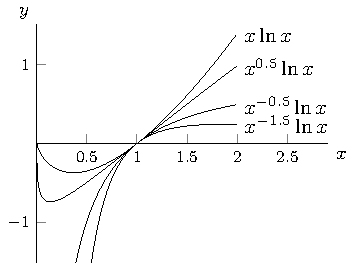
\includegraphics{figEulerCauchyABCD}
\caption*{(ب) دوسری صورت: دوہرا جذر۔}
\end{subfigure}
\begin{subfigure}{0.5\textwidth}
\centering
\begin{tikzpicture}
\begin{axis}[small,axis lines*=middle,ymin=-1.6,ymax=1.6,xmin=0,xmax=2.9,xlabel={$x$},ylabel={$y$},xlabel style={at={(axis description cs:1.05,0.5)}},ylabel style ={rotate=-90},ylabel style={at={(axis description cs:0,1.05)}}]
\addplot[domain=0.001:2,samples=100]{x^(0.1)*cos(180/pi*3*ln(x))}node[below]{$x^{0.1}\cos(3\ln x)$};
\addplot[domain=0.001:2,samples=100]{x^(0.1)*sin(180/pi*3*ln(x))}node[above]{$x^{0.1}\sin(3\ln x)$};
\end{axis}
\end{tikzpicture}
\caption*{(پ) جوڑی دار مخلوط جذر۔}
\end{subfigure}
\caption{یولر کوشی سادہ تفرقی مساوات کے حل۔}
\label{شکل_سادہ_دو_درجی_یولر_کوشی}
\end{figure}

شکل \حوالہ{شکل_سادہ_دو_درجی_یولر_کوشی} میں یولر کوشی سادہ تفرقی مساوات کی تینوں صورتوں کے حل دکھائے گئے ہیں۔

%============================
\ابتدا{مثال}\شناخت{مثال_سادہ_دو_ہم_محوری_نلکی_میدان}\quad دو ہم محوری نلکیوں کے بیچ میں ساکن برقی میدان؛ سرحدی قیمت مسئلہ\\
دو ہم محوری نلکیوں  کے بیچ میں برقی دباو تفرقی مساوات \عددی{\rho \tfrac{\dif^{\,2} v}{\dif \rho^2}+\tfrac{\dif v}{\dif \rho}=0} دیتی ہے۔نلکی کے رداس \عددی{\rho_1=\SI{2}{\centi\meter}} اور \عددی{\rho_2=\SI{5}{\centi\meter}} ہیں جبکہ ان پر \اصطلاح{برقی دباو}\فرہنگ{برقی دباو}\حاشیہب{electric voltage}\فرہنگ{voltage} \عددی{v_1=\SI{50}{\volt}} اور \عددی{v_2=\SI{0}{\volt}} ہے۔درمیانی خطے کی برقی دباو حاصل کریں۔

حل:یولر کوشی مساوات میں \عددی{a=1} اور \عددی{b=0} موجودہ تفرقی مساوات دیتا ہے۔دیے مساوات میں \عددی{v=\rho^m} پر کرتے ہوئے ذیلی مساوات \عددی{m^2=0} حاصل ہوتی ہے جس کا دوہرا جذر \عددی{m=0} ہے۔یوں عمومی  حل \عددی{v=c_1+c_2\ln x} ہو گا۔دیے گئے سرحدی شرائط حل میں پر کرتے 
\begin{align*}
50=c_1+c_2\ln 0.02, \quad 0=c_1+c_2\ln 0.05
\end{align*}
ہوئے \عددی{c_1=-163.471} اور \عددی{c_2=-54.568} حاصل ہوتے ہیں لہٰذا مخصوص حل \عددی{y=-163.471-54.568\ln \rho} ہو گا جسے شکل \حوالہ{شکل_مثال_سادہ_دو_ہم_محوری_نلکی_میدان} میں دکھایا گیا ہے۔
\begin{figure}
\centering
\begin{tikzpicture}
\begin{axis}[small,axis lines*=middle,ymin=0,ymax=58,xmin=0.02,xmax=0.056,xlabel={$\rho$},ylabel={$v$},xlabel style={at={(axis description cs:1.05,0)}},ylabel style ={rotate=-90},ylabel style={at={(axis description cs:0,1.05)}},scaled x ticks=false,xtick={0.02,0.03,0.04,0.05},xticklabels={$2$,$3$,$4$,$5$},ytick={0,50},yticklabels={$0$,$50$}]
\addplot[domain=0.01:0.05]{-163.471-54.568*ln(x)};
\end{axis}
\end{tikzpicture}
\caption{مثال \حوالہ{مثال_سادہ_دو_ہم_محوری_نلکی_میدان} کا حل۔}
\label{شکل_مثال_سادہ_دو_ہم_محوری_نلکی_میدان}
\end{figure}
\انتہا{مثال}
%==========================
\ابتدا{مثال}
یولر کوشی مساوات \حوالہ{مساوات_سادہ_دو_درجی_یولر_کوشی_الف} میں \عددی{x=e^{t}} پر کرتے ہوئے اس کو مستقل عددی سر والے سادہ تفرقی مساوات میں تبدیل کریں۔

حل:ہم \عددی{y(x)} کو \عددی{y[x(t)]} یعنی \عددی{y(t)} تصور کرتے ہیں۔یوں زنجیری تفرق سے
\begin{align*}
\frac{\dif y}{\dif x}=\frac{\dif y}{\dif t}\frac{\dif t}{\dif x}, \quad \frac{\dif^{\,2} y}{\dif x^2}=\frac{\dif^{\,2}y}{\dif t^2}\left(\frac{\dif t}{\dif x}\right)^2+\frac{\dif y}{\dif t}\frac{\dif^{\,2} t}{\dif x^2}
\end{align*}
لکھا جا سکتا ہے۔ان میں \عددی{\tfrac{\dif t}{\dif x}=\tfrac{1}{x}} اور \عددی{\tfrac{\dif^{\,2} t}{\dif x^2}=-\tfrac{1}{x^2}} پر کرتے ہیں۔
\begin{align*}
\frac{\dif y}{\dif x}=\frac{1}{x}\frac{\dif y}{\dif t}, \quad \frac{\dif^{\,2} y}{\dif x^2}=\frac{1}{x^2}\frac{\dif^{\,2}y}{\dif t^2}-\frac{1}{x^2}\frac{\dif y}{\dif t}
\end{align*}
انہیں مساوات \حوالہ{مساوات_سادہ_دو_درجی_یولر_کوشی_الف} میں پر کرتے 
\begin{align*}
x^2\left(\frac{1}{x^2}\frac{\dif^{\,2}y}{\dif t^2}-\frac{1}{x^2}\frac{\dif y}{\dif t}\right)+ax\left(\frac{1}{x}\frac{\dif y}{\dif t}\right)+by=0
\end{align*}
ہوئے مستقل عددی سر والا سادہ تفرقی مساوات حاصل ہوتا ہے  جہاں \عددی{\dot{y}=\tfrac{\dif y}{\dif t}} اور \عددی{\ddot{y}=\tfrac{\dif^{\,2}y}{\dif t^2}} ہیں۔
\begin{align}
\ddot{y}+(a-1)\dot{y}+by=0
\end{align}
\انتہا{مثال}
%==================================

\حصہء{سوالات}
سوال \حوالہ{سوال_سادہ_دو_یولر_کوشی_الف} تا سوال \حوالہ{سوال_سادہ_دو_یولر_کوشی_ب} حل کریں۔
%=======================

\ابتدا{سوال}\شناخت{سوال_سادہ_دو_یولر_کوشی_الف}
\begin{align*}
x^2y''-2xy'+2y=0
\end{align*}
جواب:\عددی{y=c_1x+c_2x^2}
\انتہا{سوال}
%====================
\ابتدا{سوال}
\begin{align*}
x^2y''-6y=0
\end{align*}
جواب:\عددی{y=c_1x^3+c_2x^{-2}}
\انتہا{سوال}
%==========================
\ابتدا{سوال}
\begin{align*}
x^2y''+6xy'+4y=0
\end{align*}
جواب:\عددی{y=\tfrac{c_1}{x}+\tfrac{c_2}{x^4}}
\انتہا{سوال}
%==================
\ابتدا{سوال}
\begin{align*}
x^2y''-5xy'+9y=0
\end{align*}
جواب:\عددی{y=(c_1+c_2\ln x)x^3}
\انتہا{سوال}
%==========================
\ابتدا{سوال}
\begin{align*}
x^2y''+11xy'+25y=0
\end{align*}
جواب:\عددی{y=(c_1+c_2\ln x)x^{-5}}
\انتہا{سوال}
%========================
\ابتدا{سوال}
\begin{align*}
10x^2y''+11xy'-3y=0
\end{align*}
جواب:\عددی{y=c_1\sqrt{x}+c_2x^{-\tfrac{3}{5}}}
\انتہا{سوال}
%=====================
\ابتدا{سوال}
\begin{align*}
x^2y''+0.44xy'+0.0748y=0
\end{align*}
جواب:\عددی{y=c_1x^{0.22}+c_2x^{0.34}}
\انتہا{سوال}
%======================
\ابتدا{سوال}
\begin{align*}
x^2y''+0.4xy'+0.73y=0
\end{align*}
جواب:\عددی{y=x^{0.3}[c_1\cos(0.8\ln x)+c_2\sin(0.8\ln x)]}
\انتہا{سوال}
%===================
\ابتدا{سوال}\شناخت{سوال_سادہ_دو_یولر_کوشی_ب}
\begin{align*}
x^2y''+2xy'+4.25y=0
\end{align*}
جواب:\عددی{y=x^{-0.5}[c_1\cos(2\ln x)+c_2\sin(2\ln x)]}
\انتہا{سوال}
%======================
سوال \حوالہ{سوال_سادہ_دو_یولر_کوشی_پ} تا سوال \حوالہ{سوال_سادہ_دو_یولر_کوشی_ت} ابتدائی قیمت مسئلے ہیں۔انہیں حل کریں۔

\ابتدا{سوال}\شناخت{سوال_سادہ_دو_یولر_کوشی_پ}
\begin{align*}
x^2y''-0.4xy'+0.45y=0,\quad y(1)=2,\quad y'(1)=-1
\end{align*}
جواب:\عددی{y=7\sqrt{x}-5x^{0.9}}
\انتہا{سوال}
%================================
\ابتدا{سوال}
\begin{align*}
x^2y''+1.08xy'-0.01713y=0,\quad y(1)=-1,\quad y'(1)=1
\end{align*}
جواب:\عددی{y=\tfrac{23}{18}x^{0.23}-\tfrac{41}{18}x^{-0.31}}
\انتہا{سوال}
%================================
\ابتدا{سوال}
\begin{align*}
35x^2y''+57xy'+3y=0,\quad y(1)=3,\quad y'(1)=-5
\end{align*}
جواب:\عددی{y=\tfrac{77}{4}x^{-\tfrac{3}{7}}-\tfrac{65}{4}x^{-\tfrac{1}{5}}}
\انتہا{سوال}
%================================
\ابتدا{سوال}
\begin{align*}
6x^2y''+19xy'+6y=0,\quad y(1)=-3,\quad y'(1)=1
\end{align*}
جواب:\عددی{y=\tfrac{6}{5}x^{-\tfrac{3}{2}}-\tfrac{21}{5}x^{-\tfrac{2}{3}}}
\انتہا{سوال}
%================================
\ابتدا{سوال}
\begin{align*}
25x^2y''-15xy'+16y=0,\quad y(2)=0,\quad y'(2)=1
\end{align*}
جواب:\عددی{y=2^{\tfrac{1}{5}}x^{\tfrac{4}{5}}(\ln x-\ln 2)}
\انتہا{سوال}
%================================
\ابتدا{سوال}\شناخت{سوال_سادہ_دو_یولر_کوشی_ت}
\begin{align*}
49x^2y''+77xy'+4y=0,\quad y(2)=3,\quad y'(2)=0
\end{align*}
جواب:\عددی{y=x^{-\tfrac{2}{7}}(2.93+1.04\ln x)}
\انتہا{سوال}
%================================

\حصہ{حل کی وجودیت اور یکتائی؛ ورونسکی}
اس حصے میں متجانس خطی سادہ تفرقی مساوات،
\begin{align}\label{مساوات_سادہ_دو_وجودیت_مخصوص_الف}
y''+p(x)y'+q(x)y=0
\end{align}
جس کے عددی سر \عددی{p(x)} اور \عددی{q(x)} کوئی بھی \اصطلاح{استمراری تفاعل} ہو سکتے  ہیں، کے عمومی حل کی \اصطلاح{وجودیت}\فرہنگ{وجودیت}\حاشیہب{existence}\فرہنگ{existence} پر غور کیا جائے گا۔ساتھ ہی ساتھ مساوات \حوالہ{مساوات_سادہ_دو_وجودیت_مخصوص_الف} اور  ابتدائی معلومات
\begin{align}\label{مساوات_سادہ_دو_وجودیت_مخصوص_ب}
y(x_0)=K_0, \quad y'(x_0)=K_1
\end{align}
کے  ابتدائی قیمت مسئلہ کی مخصوص حل کی \اصطلاح{یکتائی}\فرہنگ{یکتائی}\حاشیہب{uniqueness}\فرہنگ{uniqueness} پر بحث کی جائے گی۔ 

مسئلہ \حوالہ{مسئلہ_سادہ_دو_درجی_یکتا_مخصوص_حل} کہتا ہے کہ اس ابتدائی قیمت مسئلے کا مخصوص حل پایا جاتا ہے جو یکتا ہو گا اور مساوات \حوالہ{مساوات_سادہ_دو_وجودیت_مخصوص_الف} کے عمومی حل
\begin{align}
y=c_1y_1+c_2y_2\quad \quad \text{\RL{اختیاری $c_1$, $c_2$}}
\end{align}
میں تمام حل شامل ہیں۔یوں استمراری عددی سر والے متجانس سادہ تفرقی مساوات کا کوئی \اصطلاح{نادر حل}\فرہنگ{نادر حل}\فرہنگ{حل!نادر} نہیں پایا جاتا۔نادر حل اس حل کو کہتے ہیں جسے عمومی حل سے حاصل نہیں کیا جا سکتا ہے۔

ہمیں مستقل عددی سر والے سادہ تفرقی مساوات یا یولر کوشی سادہ تفرقی مساوات کے حل کی وجودیت اور یکتائی جاننے کی ضرورت پیش نہیں آئی چونکہ ان کے حل کے دوران ہی ایسی تمام معلومات سامنے آ جاتی ہیں۔
%================

%\theoremstyle{plain}
%\begin{theorem}[]\label{مسئلہ_سادہ_دو_درجی_یکتا_مخصوص_حل}
\ابتدا{مسئلہ}\شناخت{مسئلہ_سادہ_دو_درجی_یکتا_مخصوص_حل}\quad مسئلہ وجودیت اور یکتائی برائے ابتدائی قیمت تفرقی مساوات\فرہنگ{مسئلہ!وجودیت اور یکتائی}\\
اگر \عددی{p(x)} اور \عددی{q(x)} کسی کھلے  وقفے \عددی{I} پر استمراری ہوں اور \عددی{x_0} اس وقفے پر پایا جاتا ہو، تب مساوات \حوالہ{مساوات_سادہ_دو_وجودیت_مخصوص_الف} اور مساوات \حوالہ{مساوات_سادہ_دو_وجودیت_مخصوص_ب} پر مبنی ابتدائی قیمت مسئلے کا \عددی{I} پر  یکتا مخصوص حل \عددی{y(x)}  موجود ہے۔  
%\end{theorem}
\انتہا{مسئلہ}
%============================

وجودیت حل کی ثبوت کے لئے وہی بنیادی شرائط درکار ہیں جو صفحہ \حوالہصفحہ{مسئلہ_سادہ_اول_وجودیت} پر مسئلہ \حوالہ{مسئلہ_سادہ_اول_وجودیت} کے لئے درکار تھے۔اس کتاب میں ان پر غور نہیں کیا جائے گا۔ اگرچہ یکتائی کا ثبوت عموماً آسان ہوتا ہے لیکن موجودہ مسئلہ \حوالہ{مسئلہ_سادہ_دو_درجی_یکتا_مخصوص_حل} کے یکتائی حل کا ثبوت اتنا آسان نہیں ہے لہٰذا اس کو کتاب کے آخر میں بطور ضمیمہ \حوالہ{ضمیمہ_اضافی_ثبوت} شامل کیا گیا ہے۔ 
%==================

\جزوحصہء{خطی طور غیر تابع حل}
آپ کو حصہ \حوالہ{حصہ_سادہ_اسپرنگ_کمیت} سے یاد ہو گا کہ کھلے وقفہ \عددی{I} پر عمومی حل \اصطلاح{اساس} \عددی{y_1}، \عددی{y_2} پر مشتمل ہوتا ہے جہاں \عددی{y_1} اور \عددی{y_2} کھلے وقفے \عددی{I} پر خطی طور غیر تابع حل ہیں۔ وقفہ \عددی{I} پر معین \عددی{y_1} اور \عددی{y_2}،  وقفہ \عددی{I}  پر، اس صورت \اصطلاح{خطی طور غیر تابع}\فرہنگ{خطی طور! غیر تابع}\حاشیہب{linearly independent}\فرہنگ{linearly independent} کہلاتے ہیں جب پورے وقفے پر
\begin{align}\label{مساوات_سادہ_دو_خطی_طور_غیر_تابع_الف}
k_1 y_1+k_2 y_2=0
\end{align}
سے مراد 
\begin{align}
k_1=0, \quad k_2=0
\end{align}
ہو۔\عددی{k_1} اور \عددی{k_2} میں سے کم از کم ایک کی قیمت صفر کے برابر نہ ہونے کی صورت میں مساوات \حوالہ{مساوات_سادہ_دو_خطی_طور_غیر_تابع_الف} پر پورا اترتے ہوئے حل \عددی{y_1} اور \عددی{y_2} \اصطلاح{خطی طور تابع}\فرہنگ{خطی طور!تابع}\حاشیہب{linearly dependent}\فرہنگ{linearly dependent} کہلاتے ہیں۔اگر \عددی{k_1 \ne 0} ہو تب ہم مساوات \حوالہ{مساوات_سادہ_دو_خطی_طور_غیر_تابع_الف} کو \عددی{k_1} سے تقسیم کرتے ہوئے \عددی{y_1=-\tfrac{k_2}{k_1}y_2} لکھ سکتے ہیں جو تناسبی رشتہ ہے۔اسی طرح \عددی{k_2 \ne 0} کی صورت میں \عددی{y_2=-\tfrac{k_1}{k_2}y_1} لکھا جا سکتا ہے جو تناسبی رشتے کو ظاہر کرتی ہے۔
\begin{align}\label{مساوات_سادہ_دور_خطی_غیر_تابع_شرط}
\text{(الف)}\quad y_1=ky_2,\quad \text{(ب)}\quad y_2=l y_1 \quad \quad \text{\RL{پورے $I$ پر}}
\end{align}
اس کے برعکس خطی طور غیر تابع صورت میں ہم مساوات \حوالہ{مساوات_سادہ_دو_خطی_طور_غیر_تابع_الف} کو \عددی{k_1} (یا \عددی{k_2}) سے تقسیم نہیں کر سکتے لہٰذا  تناسبی رشتہ حاصل نہیں کیا جا سکتا۔(درج بالا مساوات میں \عددی{k=-\tfrac{k_2}{k_1}} اور \عددی{l=-\tfrac{k_1}{k_2}} لکھے گئے ہیں۔\عددی{k} یا (اور) \عددی{l} صفر بھی ہو سکتے ہیں۔) خطی طور غیر تابع اور خطی طور تابع حل کو درج ذیل طرز پر بیان کیا جا سکتا ہے۔ 
%==========================

%\begin{theorem}[خطی طور تابع اور غیر تابع حل]
\ابتدا{مسئلہ}\شناخت{مسئلہ_سادہ_دو_حل_تابع_غیر_تابع}\quad خطی طور تابع اور غیر تابع حل\فرہنگ{مسئلہ!تابع اور غیر تابع حل}\\
کھلے وقفہ \عددی{I} پر استمراری  \عددی{p(x)} اور \عددی{q(x)} عددی سر والے سادہ تفرقی  مساوات \حوالہ{مساوات_سادہ_دو_خطی_طور_غیر_تابع_الف} کے \عددی{I}  پر دو حل \عددی{y_1} اور \عددی{y_2} اس صورت خطی طور غیر تابع ہوں گے جب ان کے \اصطلاح{ورونسکی}\فرہنگ{ورونسکی}\حاشیہب{Wronskian}\فرہنگ{Wronskian}
\begin{align}\label{مساوات_سادہ_دو_ورونسکی_تعریف}
W(y_1,y_2)=y_1y_2'-y_2y_1'
\end{align}
کی قیمت  کسی \عددی{x_0} پر صفر کے برابر ہو جہاں \عددی{x_0} کھلے وقفے \عددی{I} پر پایا جاتا ہے۔مزید اگر  نقطہ \عددی{x=x_0} پر \عددی{W=0} ہو تب پورے \عددی{I} پر \عددی{W=0} ہو گا۔یوں اگر \عددی{I} پر کوئی ایسا \عددی{x} پایا جاتا ہو جس پر \عددی{W} صفر کے برابر نہ ہو تب \عددی{y_1} اور \عددی{y_2} خطی طور غیر تابع ہوں گے۔
%\end{theorem}
\انتہا{مسئلہ}
%==================
\ابتدا{ثبوت}
\begin{enumerate}
\item[(الف)]
\عددی{y_1} اور \عددی{y_2} کو \عددی{I} پر خطی طور غیر تابع تصور کریں۔یوں مساوات \حوالہ{مساوات_سادہ_دور_خطی_غیر_تابع_شرط}-الف یا ب میں سے ایک درست ہو گا۔اگر  مساوات \حوالہ{مساوات_سادہ_دور_خطی_غیر_تابع_شرط}-الف  درست ہو تب
\begin{align*}
W(y_1,y_2)=y_1y_2'-y_2y_1'=ky_2y_2'-y_2ky_2'=0
\end{align*}
ہو گا۔اسی طرح مساوات \حوالہ{مساوات_سادہ_دور_خطی_غیر_تابع_شرط}-ب کی صورت میں بھی \عددی{W=0} ملتا ہے۔
\item[(ب)]
 اس کے الٹ چلتے ہوئے ہم ثابت کرتے ہیں کہ کسی \عددی{x_0} پر \عددی{W(y_1,y_2)=0} سے مراد \عددی{y_1} اور \عددی{y_2} کا \عددی{I} پر خطی طور تابع ہونا ہے۔درج ذیل مساوات پر غور کریں جہاں \عددی{k_1} اور \عددی{k_2} کو نا معلوم متغیرات تصور کریں۔
\begin{gather}
\begin{aligned}\label{مساوات_سادہ_دو_درجی_ثبوت_الف}
k_1y_1(x_0)+k_2y_2(x_0)&=0\\
k_1y_1'(x_0)+k_2y_2'(x_0)&=0
\end{aligned}
\end{gather}
\عددی{k_2} حذف کرنے کی نیت سے  پہلی مساوات کو \عددی{y_2'(x_0)} اور دوسری کو \عددی{-y_2(x_0)} سے ضرب دیتے ہوئے دونوں کا مجموعہ لیتے ہیں۔
\begin{align}\label{مساوات_سادہ_دو_درجی_ثبوت_ب}
k_1y_1(x_0)y_2'(x_0)-k_1y_1'(x_0)y_2(x_0)=k_1W(y_1(x_0),y_2(x_0))=0
\end{align}
اسی طرح \عددی{k_1} حذف کرنے کے لئے پہلی مساوات کو \عددی{-y_1'(x_0)} اور دوسری کو \عددی{y_1(x_0)} سے ضرب دیتے ہوئے دونوں مساوات کا مجموعہ
\begin{align}\label{مساوات_سادہ_دو_درجی_ثبوت_پ}
k_2y_1(x_0)y_2'(x_0)-k_2y_2(x_0)y_1'(x_0)=k_2W(y_1(x_0),y_2(x_0))=0
\end{align}
لیتے ہیں۔اب اگر \عددی{x_0} پر \عددی{W} صفر نہ ہوتا تب ہم مساوات \حوالہ{مساوات_سادہ_دو_درجی_ثبوت_ب} اور مساوات \حوالہ{مساوات_سادہ_دو_درجی_ثبوت_پ} کو \عددی{W} سے تقسیم کرتے ہوئے \عددی{k_1=k_2=0} حاصل کرتے البتہ \عددی{x_0} پر \عددی{W(y_1(x_0),y_2(x_0))=0} ہے لہٰذا ہم ان مساوات کو \عددی{W} سے  تقسیم نہیں کر سکتے ہیں۔ یوں  ہمزاد مساوات \حوالہ{مساوات_سادہ_دو_درجی_ثبوت_الف} کا حل \عددی{k_1} اور \عددی{k_2} پایا جاتا ہے جہاں \عددی{k_1} اور \عددی{k_2} دونوں غیر صفر ہو سکتے ہیں۔ اب ان اعداد \عددی{k_1} اور \عددی{k_2} کو استعمال کرتے ہوئے تفاعل
\begin{align}
y(x)=k_1y_1(x)+k_2y_2(x)
\end{align}
لیتے ہیں۔چونکہ مساوات \حوالہ{مساوات_سادہ_دو_وجودیت_مخصوص_الف} متجانس خطی ہے لہٰذا  مسئلہ \حوالہ{مسئلہ_دو_درجی_خطی_میل}  (مسئلہ خطی میل) کے تحت  یہ تفاعل بھی مساوات \حوالہ{مساوات_سادہ_دو_وجودیت_مخصوص_الف} کا حل ہو گا۔مساوات \حوالہ{مساوات_سادہ_دو_درجی_ثبوت_الف} سے ظاہر ہے کہ یہ تفاعل ابتدائی معلومات \عددی{y(x_0)=0} اور \عددی{y'(x_0)=0} پر پورا اترتا ہے۔اب تصور کریں کہ مساوات \حوالہ{مساوات_سادہ_دو_وجودیت_مخصوص_الف} کا دوسرا حل جو انہیں  ابتدائی معلومات پر پورا اترتا ہو \عددی{y^*(x)=0} ہے۔اب چونکہ مساوات \حوالہ{مساوات_سادہ_دو_وجودیت_مخصوص_الف} میں \عددی{p(x)} اور \عددی{q(x)} استمراری ہیں لہٰذا مسئلہ \حوالہ{مسئلہ_سادہ_دو_درجی_یکتا_مخصوص_حل} کے تحت اس کا مخصوص حل یکتا ہو گا۔یوں \عددی{y(x)} اور \عددی{y^*(x)} مختلف نہیں ہو سکتے ہیں لہٰذا \عددی{y^*(x)=y(x)=0} یعنی
\begin{align}\label{مساوات_سادہ_دو_درجی_ثبوت_ت}
k_1y_1+k_2y_2\equiv 0\quad \quad \text{\RL{پورے $I$ پر}}
\end{align}
ہو گا۔چونکہ \عددی{k_1} اور \عددی{k_2} میں کم از کم ایک صفر کے برابر نہیں ہے لہٰذا  مساوات \حوالہ{مساوات_سادہ_دو_درجی_ثبوت_ت} کہتا ہے کہ \عددی{I} پر \عددی{y_1} اور \عددی{y_2} خطی طور تابع ہیں۔
\item[(پ)]
ہم مسئلے کا آخری نقطہ ثابت کرتے ہیں۔اگر کھلے وقفے \عددی{I} پر نقطہ \عددی{x_0} پر \عددی{W(x_0)=0} ہو تب ثبوت (ب) کے تحت \عددی{I} پر \عددی{y_1} اور \عددی{y_2} خطی طور تابع ہیں لہٰذا ثبوت (الف) کے تحت \عددی{W \equiv 0} ہو گا۔یوں خطی طور تابع صورت میں ایسا نہیں ہو سکتا ہے کہ \عددی{W(x_1) \ne 0} ہو جہاں \عددی{x_1} کھلے وقفہ \عددی{I} پر پایا جاتا ہے۔اگر ایسا ممکن ہو تب اس سے مراد خطی طور غیر تابع صورت ہو گی جیسا کہ دعویٰ کیا گیا ہے۔ 
\end{enumerate}
\انتہا{ثبوت}
%=================

حساب کی نقطہ نظر سے  مساوات \حوالہ{مساوات_سادہ_دو_ورونسکی_تعریف} سے درج ذیل زیادہ آسان مساوات ہے۔
\begin{align}\label{مساوات_سادہ_دو_آسان_ورونسکی}
W(y_1,y_2)=
\begin{cases}
\left(\frac{y_2}{y_1}\right)^{\!'}y_1^2  &(y_1 \ne 0)\\[0.5em]
-\left(\frac{y_1}{y_2}\right)^{\!'}y_2^2 & (y_2 \ne 0)
\end{cases}
\end{align}
آپ دیکھ سکتے ہیں کہ  ورونسکی کو قالب کی مقطع کے طرز پر لکھا جا سکتا ہے جس کو \اصطلاح{ورونسکی مقطع}\فرہنگ{ورونسکی!مقطع}\فرہنگ{مقطع!ورونسکی}\حاشیہب{Wronskian determinant}\فرہنگ{Wronskian determinant} یا حل \عددی{y_1} اور \عددی{y_2} کی \اصطلاح{ورونسکی} کہتے ہیں۔ 
\begin{align}
W(y_1,y_2)=
\begin{vmatrix}
y_1 &y_2\\[0.25em]
y_1' & y_2'
\end{vmatrix}
=y_1y_2'-y_2y_1'
\end{align}
%==============================

\ابتدا{مثال}\quad مسئلہ \حوالہ{مسئلہ_سادہ_دو_حل_تابع_غیر_تابع} کا اطلاق\\
تفرقی مساوات \عددی{y''+\omega^2y=0} کے حل \عددی{y_1=\cos \omega x} اور \عددی{y_2=\sin \omega x}  ہیں۔ان کی ورونسکی
\begin{align*}
W(\cos \omega x,\sin \omega x)=
\begin{vmatrix}
\cos \omega x &\sin \omega x\\[0.25em]
-\omega \sin \omega x & -\omega \cos \omega x
\end{vmatrix}
=\omega \cos^2 \omega x+\omega \sin^2 \omega x=\omega
\end{align*}
ہے۔مسئلہ \حوالہ{مسئلہ_سادہ_دو_حل_تابع_غیر_تابع} کے تحت یہ حل صرف اس صورت میں خطی طور غیر تابع ہوں گے جب \عددی{\omega \ne 0} ہو۔یہی دونوں حل کے حاصل تقسیم \عددی{\tfrac{y_2}{y_1}=\tan \omega x} سے بھی اخذ کیا جا سکتا ہے جہاں \عددی{\omega=0} سے \عددیء{y_2=0} ملتا ہے جو خطی طور تابع صورت ظاہر کرتی ہے۔
\انتہا{مثال}
%=============================
\ابتدا{مثال}\quad دوہرا جذر کی صورت میں مسئلہ \حوالہ{مسئلہ_سادہ_دو_حل_تابع_غیر_تابع} کا اطلاق\\
تفرقی مساوات \عددی{y''-6y'+9y=0} کا (ثابت کریں کہ) عمومی حل  \عددی{y=(c_1+c_2 x)e^{3x}}   ہے جس کا ورونسکی صفر کے برابر نہیں ہے لہٰذا \عددی{e^{3x}} اور \عددی{xe^{3x}} تمام \عددی{x} پر خطی طور غیر تابع ہیں۔
\begin{align*}
W(e^{3x},xe^{3x})=
\begin{vmatrix}
e^{3x}& xe^{3x}\\[0.25em]
3e^{3x}&e^{3x}+3xe^{3x}
\end{vmatrix}
=e^{6x}+3xe^{6x}-3xe^{6x}=e^{6x} \ne 0
\end{align*}
\انتہا{مثال}
%==================

\جزوحصہء{مساوات \حوالہ{مساوات_سادہ_دو_وجودیت_مخصوص_الف} کے عمومی حل میں تمام حل کی شمولیت}
اس حصے کو مساوات \حوالہ{مساوات_سادہ_دو_وجودیت_مخصوص_الف} کے عمومی حل کی وجودیت سے شروع کرتے ہیں۔
%=========================

\ابتدا{مسئلہ}\شناخت{مسئلہ_سادہ_دو_وجودیت_الف}\quad \اصطلاح{وجودیت عمومی حل}\فرہنگ{وجودیت!عمومی حل}\فرہنگ{حل!وجودیت عمومی حل}\فرہنگ{existence!solution}\فرہنگ{مسئلہ!وجودیت عمومی حل}\\
کھلے وقفہ \عددی{I} پر استمراری \عددی{p(x)} اور \عددی{q(x)} کی صورت میں مساوات \حوالہ{مساوات_سادہ_دو_وجودیت_مخصوص_الف} کا عمومی حل \عددی{I} پر موجود ہے۔
\انتہا{مسئلہ}
%=====================

\ابتدا{ثبوت}
مسئلہ \حوالہ{مسئلہ_سادہ_دو_درجی_یکتا_مخصوص_حل} کے تحت  \عددی{I} پر مساوات \حوالہ{مساوات_سادہ_دو_وجودیت_مخصوص_الف} کا، ابتدائی معلومات 
\begin{align*}
y_1(x_0)=1, \quad y_1'(x_0)=0
\end{align*}
پر پورا اترتا ہوا  حل  \عددی{y_1(x)} موجود ہے۔اسی طرح ابتدائی معلومات
\begin{align*}
y_2(x_0)=0, \quad y_2'(x_0)=1
\end{align*}
 پر پورا اترتا ہوا  حل \عددی{y_2(x)} بھی موجود ہے۔نقطہ \عددی{x_0} پر ان کا ورونسکی
\begin{align*}
W(y_1(x_0),y_2(x_0))=y_1(x_0)y'_2(x_0)-y_2(x_0)y'_1(x_0)=1
\end{align*}
ہے۔مسئلہ \حوالہ{مسئلہ_سادہ_دو_حل_تابع_غیر_تابع} کے تحت \عددی{I} پر \عددی{y_1} اور \عددی{y_2} خطی طور غیر تابع ہیں لہٰذا یہ مساوات \حوالہ{مساوات_سادہ_دو_وجودیت_مخصوص_الف} کے حل کی اساس ہیں۔اس طرح ثابت ہوا کہ  \عددی{I} پر  مساوات \حوالہ{مساوات_سادہ_دو_وجودیت_مخصوص_الف} کا عمومی حل \عددی{y=c_1y_1+c_2y_2} ہے جہاں \عددی{c_1} اور \عددی{c_2} اختیاری مستقل ہیں۔
\انتہا{ثبوت}
%=======================

آئیں اب ثابت کریں کہ عمومی حل اتنا عمومی ہے جتنا کوئی حل عمومی ہو سکتا ہے۔
%=====================

\ابتدا{مسئلہ}\quad عمومی حل میں تمام حل شامل ہیں\\
کھلا وقفہ \عددی{I} پر استمراری \عددی{p(x)} اور \عددی{q(x)} کی صورت میں \عددی{I} پر مساوات \حوالہ{مساوات_سادہ_دو_وجودیت_مخصوص_الف} کے ہر حل
 \عددی{y=Y(x)} کو
\begin{align}
Y(x)=C_1y_1+C_2y_2
\end{align}
لکھا جا سکتا ہے، جہاں \عددی{y_1} اور \عددی{y_2} کھلے وقفہ \عددی{I} پر مساوات \حوالہ{مساوات_سادہ_دو_وجودیت_مخصوص_الف} کی کوئی بھی اساس اور \عددی{C_1}، \عددی{C_2} مناسب مستقل ہیں۔

یوں مساوات \حوالہ{مساوات_سادہ_دو_وجودیت_مخصوص_الف} کا کوئی \اصطلاح{نادر حل}\فرہنگ{نادر حل} موجود نہیں ہے۔(نادر حل سے مراد ایسا حل ہے جس کو عمومی حل سے حاصل نہیں کیا جا سکتا ہے۔)
\انتہا{مسئلہ}
%======================

\ابتدا{ثبوت}
تصور کریں کہ \عددی{I} پر مساوات \حوالہ{مساوات_سادہ_دو_وجودیت_مخصوص_الف} کا  \عددی{y=Y(x)} کوئی حل ہے۔اب مسئلہ \حوالہ{مسئلہ_سادہ_دو_وجودیت_الف} کے تحت \عددی{I} پر  تفرقی مساوات \حوالہ{مساوات_سادہ_دو_وجودیت_مخصوص_الف} کا عمومی حل
\begin{align}\label{مساوات_سادہ_دو_ثبوت_مسئلہ_چار_الف}
y(x)=c_1y_1(x)+c_2y_2(x)
\end{align}
موجود ہے۔ہم \عددی{c_1} اور \عددی{c_2} کی وہ قیمتیں دریافت کرنا چاہتے ہیں جن سے \عددی{I} پر  \عددی{y(x)=Y(x)} حاصل ہوتا ہو۔ہم \عددی{I} پر کوئی بھی \عددی{x_0} چنتے ہوئے پہلے ثابت کرتے ہیں کہ \عددی{c_1} اور \عددی{c_2} کی ایسی قیمتیں دریافت کی جا سکتی ہیں کہ \عددی{x_0} پر \عددی{y(x_0)=Y(x_0)} اور 
\عددی{y'(x_0)=Y'(x_0)} ہوں۔اس کو مساوات \حوالہ{مساوات_سادہ_دو_ثبوت_مسئلہ_چار_الف} کے استعمال سے 
\begin{align}
c_1y_1(x_0)+c_2y_2(x_0)&=Y(x_0)\label{مساوات_سادہ_دو_ثبوت_مسئلہ_چار_ب}\\
c_1y'_1(x_0)+c_2y'_2(x_0)&=Y'(x_0)\label{مساوات_سادہ_دو_ثبوت_مسئلہ_چار_پ}
\end{align}
لکھ سکتے ہیں۔ان ہمزاد مساوات سے \عددی{c_1} اور \عددی{c_2} معلوم کرتے ہیں۔مساوات \حوالہ{مساوات_سادہ_دو_ثبوت_مسئلہ_چار_ب} کو \عددی{y'_2(x_0)} اور مساوات \حوالہ{مساوات_سادہ_دو_ثبوت_مسئلہ_چار_پ} کو \عددی{-y_2(x_0)} سے ضرب دیتے ہوئے مجموعہ لینے سے \عددی{c_1} حاصل کیا جا سکتا ہے۔ایسا کرنے سے مساوات \حوالہ{مساوات_سادہ_دو_ثبوت_مسئلہ_چار_ت} ملتی ہے۔اسی طرح \عددی{c_2} حاصل کرنے کی خاطر پہلی مساوات کو \عددی{-y'_1(x_0)} اور دوسری کو \عددی{y_1(x_0)} سے ضرب دیتے ہوئے مجموعہ لیتے ہوئے مساوات \حوالہ{مساوات_سادہ_دو_ثبوت_مسئلہ_چار_ٹ} حاصل ہوتی ہے۔ان مساوات میں \عددی{y_1}، \عددی{y'_1}، \عددی{y_2}،\عددی{y'_2}، \عددی{Y} اور \عددی{Y'} کی قیمتیں نقطہ \عددی{x_0} پر لی گئی ہیں۔ 
\begin{align}
c_1y_1y'_2-c_1y_2y'_1&=c_1W(y_1,y_2)=Yy_2'-y_2Y\label{مساوات_سادہ_دو_ثبوت_مسئلہ_چار_ت}\\
c_2y_1y'_2-c_2y_2y'_1&=c_2W(y_1,y_2)=y_1Y-Yy'_1\label{مساوات_سادہ_دو_ثبوت_مسئلہ_چار_ٹ}
\end{align}
اب چونکہ \عددی{y_1} اور \عددی{y_2} حل کی اساس ہیں لہٰذا ورونسکی کی قیمت صفر کے برابر نہیں ہے لہٰذا ان مساوات سے \عددی{c_1} اور \عددی{c_2} حاصل کیے جا سکتے ہیں
\begin{align*}
c_1=\frac{Yy_2'-y_2Y}{W}=C_1, \quad c_2=\frac{y_1Y-Yy'_1}{W}=C_2
\end{align*}
جہاں ان منفرد قیمتوں کو \عددی{C_1} اور \عددی{C_2} لکھا گیا ہے۔ انہیں مساوات \حوالہ{مساوات_سادہ_دو_ثبوت_مسئلہ_چار_الف} میں پر کرتے ہوئے مخصوص حل
\begin{align*}
y^*(x)=C_1y_1(x)+C_2y_2(x)
\end{align*}
حاصل ہوتا ہے۔اب چونکہ \عددی{C_1} اور \عددی{C_2} مساوات \حوالہ{مساوات_سادہ_دو_ثبوت_مسئلہ_چار_ب} اور مساوات \حوالہ{مساوات_سادہ_دو_ثبوت_مسئلہ_چار_پ} کے حل ہیں لہٰذا ہم ان مساوات سے دیکھتے ہیں کہ
\begin{align*}
y^{*}(x_0)=Y(x_0),\quad y^{*'}(x_0)=Y'(x_0)
\end{align*}
مسئلہ \حوالہ{مسئلہ_سادہ_دو_درجی_یکتا_مخصوص_حل} میں جس یکتائی کا ذکر کیا گیا ہے اس کے تحت \عددی{y^*} اور \عددی{Y} تمام \عددی{I} پر ہر جگہ برابر ہوں گے۔
\انتہا{ثبوت}
%=========================

\حصہء{سوالات}
%===================

\ابتدا{سوال}
مساوات \حوالہ{مساوات_سادہ_دو_آسان_ورونسکی} سے مساوات \حوالہ{مساوات_سادہ_دو_ورونسکی_تعریف} حاصل کریں۔
\انتہا{سوال}
%===========================
سوال \حوالہ{سوال_سادہ_ورونسکی_الف} تا سوال \حوالہ{سوال_سادہ_ورونسکی_ب} کی ورونسکی حاصل کریں۔حاصل تقسیم سے ثابت کریں کہ یہ خطی طور غیر تابع ہیں اور مسئلہ \حوالہ{مسئلہ_سادہ_دو_حل_تابع_غیر_تابع} سے  بھی اس بات کی تصدیق کریں

%======================
\ابتدا{سوال}\شناخت{سوال_سادہ_ورونسکی_الف}\quad $e^{2x}, e^{-1.2x}$\\
جوابات:\عددی{\tfrac{e^{2x}}{e^{-1.2x}}=e^{3.2x} \ne c}، \عددی{W=-3.2e^{0.8x}\ne 0}
\انتہا{سوال}
%============================ 
\ابتدا{سوال}\quad $e^{2.4x}, e^{1.1x}$\\
جوابات:\عددی{\tfrac{y_1}{y_2}=e^{1.3x} \ne c}، \عددی{W=-1.3e^{3.5x} \ne 0}
\انتہا{سوال}
%===============
\ابتدا{سوال}\quad
$x, \frac{1}{x}$\\
جوابات:\عددی{\tfrac{y_1}{y_2}=x^2 \ne c}، \عددی{W=-2x^{-2} \ne 0}
\انتہا{سوال}
%=====================
\ابتدا{سوال}\quad
$x, x^3$\\
جوابات:\عددی{\tfrac{y_1}{y_2}=x^{-2} \ne c}، \عددی{W=2x^3 \ne 0}
\انتہا{سوال}
%===================
\ابتدا{سوال}\quad
$e^{-0.2x}\sin 3x, e^{-0.2x} \cos 3x$\\
جوابات:\عددی{\tfrac{y_1}{y_2}=\tan 3x \ne c}، \عددی{W=3e^{-0.4x} \ne 0}
\انتہا{سوال}
%========================
\ابتدا{سوال}\quad
$e^{-ax}\sinh kx, e^{-ax} \cosh kx$\\
جوابات:\عددی{\tfrac{y_1}{y_2}=\tanh kx \ne c}، \عددی{W=-ke^{-2ax} \ne 0}
\انتہا{سوال}
%============================
\ابتدا{سوال}\شناخت{سوال_سادہ_ورونسکی_ب}\quad
$x^{a}\sin(k\ln x), x^{a}\cos(k\ln x)$\\
جوابات:\عددی{\tfrac{y_1}{y_2}=\tan(k \ln x) \ne c}، \عددی{W=-kx^{2a-1} \ne 0}
\انتہا{سوال}
%===========================

سوال \حوالہ{سوال_سادہ_ورونسکی_پ} تا سوال \حوالہ{سوال_سادہ_ورونسکی_ت} میں تفرقی مساوات کے حل دیے گئے ہیں۔تفرقی مساوات حاصل کریں۔ورونسکی کی مدد سے ثابت کریں کہ دیے گئے حل خطی طور غیر تابع ہیں اور ابتدائی قیمت مسئلے کا مخصوص حل حاصل کریں۔
%==============================

\ابتدا{سوال}\شناخت{سوال_سادہ_ورونسکی_پ}\quad 
$\sin 3x, \, \cos 3x,\quad y(0)=2,\quad y'(0)=-3 $\\
جوابات:\عددی{y''+9y=0}، \عددی{W=-3\ne 0}، \عددی{y=2\cos 3x-\sin 3x}
\انتہا{سوال}
%===========================
\ابتدا{سوال}\quad 
$x^3, \, x^{-4},\quad y(1)=-1,\quad y'(1)=2 $\\
جوابات:\عددی{x^2y''+2xy'-12y=0}، \عددی{W=-\tfrac{7}{x^2}\ne 0}، \عددی{y=-\tfrac{2x^3}{7}-\tfrac{5x^{-4}}{7}}
\انتہا{سوال}
%===========================
\ابتدا{سوال}\quad 
$e^{-1.2x}\sin 0.8x, \, e^{-1.2x}\cos 0.8 x,\quad y(0)=5,\quad y'(0)=7 $\\
جوابات:\عددی{y''+2.4y'+2.08y=0}، \عددی{W=-0.8e^{-2.4x} \ne 0}، \\
\عددی{y=e^{-\tfrac{6}{5}x}(\tfrac{65}{4}\sin\tfrac{4x}{5}+5\cos\tfrac{4x}{5})}
\انتہا{سوال}
%===========================
\ابتدا{سوال}\quad 
$x^3,\, x^3\ln x,\quad y(1)=2,\quad y'(1)=8 $\\
جوابات:\عددی{x^2y''-5xy'+9y=0}، \عددی{W=x^5 \ne 0}، \عددی{y=2x^3(1+\ln x)}
\انتہا{سوال}
%===========================
\ابتدا{سوال}\quad 
$1,\, e^{3x},\quad y(0)=1.5,\quad y'(0)=-2.5 $\\
جوابات:\عددی{y''-3y'=0}، \عددی{W=3e^{3x} \ne 0}، \عددی{y=\tfrac{8}{3}e^{3x}-\tfrac{2}{3}}
\انتہا{سوال}
%===========================
\ابتدا{سوال}\quad 
$e^{-kx}\sin \pi x, \, e^{-kx}\cos \pi x,\quad y(0)=1,\quad y'(0)=-k-\pi $\\
جوابات:\عددی{y''+2ky'+(k^2+\pi^2)y=0}، \عددی{W=-\pi e^{-2kx} \ne 0}، \\
\عددی{y=e^{-kx}(\sin \pi x-\cos \pi x)}
\انتہا{سوال}
%===========================
\ابتدا{سوال}\شناخت{سوال_سادہ_ورونسکی_ت}\quad 
$\sinh 1.8x, \,\cosh 1.8x,\quad y(0)=14.2,\quad y'(0)=16.38 $\\
جوابات:\عددی{y''-3.24y=0}، \عددی{W=-1.8 \ne 0}، \\
\عددی{y=9.1\sinh 1.8x+14.2\cosh 1.8x}
\انتہا{سوال}
%===========================
\ابتدا{سوال}
تفرقی مساوات \عددی{y''-y=0} کا عمومی حل قوت نمائی تفاعل اور \اصطلاح{بذلولی}\فرہنگ{بذلولی}\حاشیہب{hyperbolic}\فرہنگ{hyperbolic!function} تفاعل کی صورت میں لکھیں۔دونوں صورتوں کے مستقل کا تعلق کیا ہے؟

جوابات:\عددی{y=c_1e^{x}+c_2e^{-x}}، \عددی{y=c_a\sinh x+c_b\cosh x}، \عددی{c_a=c_1-c_2}، \عددی{c_b=c_1+c_2}
\انتہا{سوال}
%=============================
%=====================================

\حصہ{غیر متجانس سادہ تفرقی مساوات}\شناخت{حصہ_سادہ_دو_غیر_متجانس}
اس باب میں اب تک متجانس خطی سادہ تفرقی مساوات پر غور کیا گیا۔یہاں سے باب کے اختتام تک غیر متجانس خطی سادہ تفرقی مساوات پر غور کیا جائے گا۔درج ذیل غیر متجانس خطی تفرقی مساوات پر غور کرتے ہیں جہاں \عددی{r \not \equiv 0} ہے۔
\begin{align}\label{مساوات_سادہ_دو_غیر_متجانس_الف}
y''+p(x)y'+q(x)y=r(x)
\end{align}
ہم دیکھیں گے کہ مساوات \حوالہ{مساوات_سادہ_دو_غیر_متجانس_الف} کا عمومی حل، مطابقتی متجانس مساوات 
\begin{align}\label{مساوات_سادہ_دو_غیر_متجانس_ب}
y''+p(x)y'+q(x)y=0
\end{align}
کے عمومی حل اور مساوات \حوالہ{مساوات_سادہ_دو_غیر_متجانس_ب} کے ایک مخصوص حل کا مجموعہ ہو گا۔ مساوات \حوالہ{مساوات_سادہ_دو_غیر_متجانس_الف} کے عمومی حل اور مخصوص حل کی تعریف درج ذیل ہے۔
%==============

\ابتدا{تعریف}\quad عمومی حل اور مخصوص حل\\
کھلے وقفہ \عددی{I} پر غیر متجانس  مساوات \حوالہ{مساوات_سادہ_دو_غیر_متجانس_الف} کا عمومی حل
\begin{align}\label{مساوات_سادہ_دو_غیر_متجانس_پ}
y(x)=y_h(x)+y_p(x)
\end{align}
ہو گا جہاں \عددی{I} پر \عددی{y_h=c_1y_1+c_2y_2} متجانس مساوات \حوالہ{مساوات_سادہ_دو_غیر_متجانس_ب} کا عمومی حل ہے اور \عددی{I} پر \عددی{y_p} مساوات \حوالہ{مساوات_سادہ_دو_غیر_متجانس_الف} کا کوئی بھی حل ہے جس میں مستقل نہیں پایا جاتا۔

مساوات \حوالہ{مساوات_سادہ_دو_غیر_متجانس_الف} کا مخصوص حل، مساوات \حوالہ{مساوات_سادہ_دو_غیر_متجانس_پ} کے  \عددی{c_1} اور \عددی{c_2} میں خصوصی قیمتیں پر کرتے ہوئے حاصل کیا جاتا ہے۔
\انتہا{تعریف}
%=========================

اب ہمیں حل کی ان تعریف کا جواز پیش کرنا ہو گا اور ساتھ ہی ساتھ مساوات \حوالہ{مساوات_سادہ_دو_غیر_متجانس_الف} کا  حل \عددی{y_p} حاصل کرنا ہو گا۔پس ہم پہلے ثابت کرتے ہیں کہ مساوات \حوالہ{مساوات_سادہ_دو_غیر_متجانس_پ} کا عمومی حل مساوات \حوالہ{مساوات_سادہ_دو_غیر_متجانس_الف} پر پورا اترتا ہے اور یہ کہ مساوات \حوالہ{مساوات_سادہ_دو_غیر_متجانس_الف} اور مساوات \حوالہ{مساوات_سادہ_دو_غیر_متجانس_ب} کے حل کا آپس میں سادہ تعلق ہے۔
%=================

\ابتدا{مسئلہ}\شناخت{مسئلہ_سادہ_دو_حل_تعلق}\quad مساوات \حوالہ{مساوات_سادہ_دو_غیر_متجانس_الف} اور مساوات \حوالہ{مساوات_سادہ_دو_غیر_متجانس_ب} کے حل کا آپس میں تعلق\\
\begin{enumerate}
\item[(الف)]
کھلے وقفہ \عددی{I} پر مساوات \حوالہ{مساوات_سادہ_دو_غیر_متجانس_الف} کے حل \عددی{y} اور اسی وقفے پر مساوات \حوالہ{مساوات_سادہ_دو_غیر_متجانس_ب} کے حل \عددیء{\tilde{y}} کا مجموعہ \عددی{I} پر مساوات \حوالہ{مساوات_سادہ_دو_غیر_متجانس_الف} کا حل ہے۔بالخصوص مساوات \حوالہ{مساوات_سادہ_دو_غیر_متجانس_پ} کھلے وقفہ \عددی{I} پر مساوات \حوالہ{مساوات_سادہ_دو_غیر_متجانس_الف} کا حل ہو گا۔
\item[(ب)]
کھلے وقفہ \عددی{ِI} پر مساوات \حوالہ{مساوات_سادہ_دو_غیر_متجانس_الف} کے دو حل کا فرق \عددی{I} پر مساوات \حوالہ{مساوات_سادہ_دو_غیر_متجانس_ب} کا حل ہے۔ 
\end{enumerate}
\انتہا{مسئلہ}
%======================

\ابتدا{ثبوت}
\begin{enumerate}
\item[(الف)]
مساوات \حوالہ{مساوات_سادہ_دو_غیر_متجانس_الف} کے بائیں ہاتھ کو \عددی{L[y]} سے ظاہر کرتے ہیں۔یوں  \عددی{I} پر مساوات \حوالہ{مساوات_سادہ_دو_غیر_متجانس_الف} کے کسی بھی حل \عددی{y} اور مساوات \حوالہ{مساوات_سادہ_دو_غیر_متجانس_ب} کے کسی بھی حل \عددی{\tilde{y}} کے لئے درج ذیل لکھا جا سکتا ہے۔
\begin{align*}
L[y+\tilde{y}]=L[y]+L[\tilde{y}]=r+0=r
\end{align*}
\item[(ب)]
کھلے وقفے \عددی{I} پر مساوات \حوالہ{مساوات_سادہ_دو_غیر_متجانس_الف} کے کسی بھی حل \عددی{y} اور \عددی{y^*} کے لئے درج ذیل لکھا جا سکتا ہے۔
\begin{align*}
L[y-y^*]=L[y]-L[y^*]=r-r=0
\end{align*}
\end{enumerate}
\انتہا{ثبوت}
%=======================

ہم جانتے ہیں کہ متجانس مساوات \حوالہ{مساوات_سادہ_دو_غیر_متجانس_ب} کے عمومی حل میں تمام حل شامل ہوتے ہیں۔اب ہم ثابت کرتے ہیں کہ غیر متجانس مساوات \حوالہ{مساوات_سادہ_دو_غیر_متجانس_الف} کے عمومی حل میں اس کے تمام حل شامل ہیں۔
%===================

\ابتدا{مسئلہ}\quad غیر متجانس سادہ تفرقی مساوات کے عمومی حل میں تمام حل شامل ہیں\\
کھلے وقفہ \عددی{I} پر استمراری \عددی{p(x)}، \عددی{q(x)} اور \عددی{r(x)} کی صورت میں \عددی{I} پر مساوات \حوالہ{مساوات_سادہ_دو_غیر_متجانس_الف} کا ہر حل،  مساوات \حوالہ{مساوات_سادہ_دو_غیر_متجانس_پ} میں دیے گئے عمومی حل کے اختیاری مستقل \عددی{c_1} اور \عددی{c_2} میں موزوں قیمتیں پر کرنے سے حاصل کیا جاتا ہے۔ 
\انتہا{مسئلہ}
%=====================

\ابتدا{ثبوت}
کھلے وقفے \عددی{I} پر \عددی{y^*} مساوات \حوالہ{مساوات_سادہ_دو_غیر_متجانس_الف} کا کوئی حل ہے جبکہ \عددی{x_0} اس وقفے پر کوئی \عددی{x} ہے۔اسی طرح مساوات \حوالہ{مساوات_سادہ_دو_غیر_متجانس_پ} کھلے وقفے پر مساوات \حوالہ{مساوات_سادہ_دو_غیر_متجانس_الف} کا کوئی عمومی حل ہے۔یہ حل موجود ہے۔یقیناً \عددی{y_h=c_1y_1+c_2y_2} مسئلہ \حوالہ{مسئلہ_سادہ_دو_وجودیت_الف} کے تحت موجود ہے جبکہ \عددی{y_p} کی وجودیت اس باب میں آگے جا کر  دکھائی جائے گی۔اب مسئلہ \حوالہ{مسئلہ_سادہ_دو_حل_تعلق}-ب کے تحت  \عددی{Y=y^*-y_p} کھلے وقفے پر مساوات \حوالہ{مساوات_سادہ_دو_غیر_متجانس_ب} کا حل ہے۔نقطہ \عددی{x_0} پر
\begin{align*}
Y(x_0)=y^*(x_0)-y_p(x_0), \quad Y'(x_0)=y^{*'}(x_0)-y_p'(x_0)
\end{align*}
لکھا جا سکتا ہے۔کھلے وقفے  \عددی{I} پر، مسئلہ \حوالہ{مسئلہ_سادہ_دو_درجی_یکتا_مخصوص_حل} کے مطابق، کسی بھی ابتدائی معلومات کی طرح، ان معلومات پر پورا اترتا ہوا، مساوات \حوالہ{مساوات_سادہ_دو_غیر_متجانس_ب} کا مخصوص حل موجود ہے جسے \عددی{y_h} میں \عددی{c_1} اور \عددی{c_2} میں موزوں  قیمتیں پر کرنے سے حاصل کیا جا سکتا ہے۔  اس حقیقت کو مد نظر رکھتے ہوئے  \عددی{y^*=Y+y_p} سے مسئلہ کا دعویٰ ثابت ہوتا ہے۔
\انتہا{ثبوت}
%======================
%========================
\جزوحصہء{نا معلوم عددی سر کی ترکیب}
آپ نے دیکھا کہ مساوات \حوالہ{مساوات_سادہ_دو_غیر_متجانس_الف} یا اس پر مبنی ابتدائی قیمت مسئلے کا حل  حاصل کرنے کی خاطر مساوات \حوالہ{مساوات_سادہ_دو_غیر_متجانس_ب} کو حل کرنا ہو گا اور مساوات \حوالہ{مساوات_سادہ_دو_غیر_متجانس_الف} کا کوئی بھی حل \عددی{y_p}  تلاش کرنا ہو گا۔اس طرح عمومی حل \حوالہ{مساوات_سادہ_دو_غیر_متجانس_پ} حاصل ہو گا۔

مساوات \حوالہ{مساوات_سادہ_دو_غیر_متجانس_الف} کا حل \عددی{y_p} حاصل کرنے کی ایک ترکیب کو \اصطلاح{نا معلوم عددی سر کی ترکیب}\فرہنگ{نا معلوم عددی سر!ترکیب}\حاشیہب{method of undetermined coefficients}\فرہنگ{coefficients!undetermined method}  کہتے ہیں۔یہ ترکیب نہایت آسان ہے۔ اس ترکیب سے ارتعاشی نظام عمدگی سے حل ہوتے ہیں لہٰذا اسے انجینئری شعبے میں مقبولیت حاصل ہے۔اس باب کے آخری حصے میں عمومی ترکیب پر غور کیا جائے گا جو نسبتاً مشکل ترکیب ہے۔

نا معلوم عددی سر کی ترکیب ان خطی سادہ تفرقی مساوات
\begin{align}\label{مساوات_سادہ_دو_نا_معلوم_الف}
y''+ay'+by=r(x)
\end{align}
 کے حل کے لئے موزوں ہے جس کے عددی سر \عددی{a} اور \عددی{b} مستقل مقدار ہوں اور \عددی{r(x)} قوت نمائی تفاعل ہو یا \عددی{x} کی طاقت ہو یا  سائن نما تفاعل ہو اور یا ان تفاعل کا مجموعہ یا حاصل ضرب ہو۔ایسی تفاعل کی تفرقات بھی یہی تفاعل ہوتی ہیں۔مثلاً \عددی{x^3} کے تفرقات   \عددی{3x^2}، \عددی{6x} اور \عددی{6} ہیں جو از خود \عددی{x} کی طاقت ہیں۔اسی طرح \عددی{\sin \omega x} کا ایک درجی تفرق \عددی{\omega \cos \omega x} جبکہ دو درجی تفرق \عددی{-\omega^2\sin\omega x} ہے۔یہ دونوں تفرقات از خود  سائن نما تفاعل ہیں۔

اس ترکیب میں \عددی{y_p} کو \عددی{r(x)} اور اس کے تمام تفرقات کے مجموعے کی صورت میں  لکھا جاتا ہے۔مجموعہ لکھتے ہوئے ہر رکن کو نا معلوم مستقل سے ضرب دیا جاتا ہے۔ \عددی{y_p} اور اس کے تفرقات کو  مساوات \حوالہ{مساوات_سادہ_دو_نا_معلوم_الف} میں پر کرتے ہوئے دونوں اطراف کے یکساں اجزاء کے عددی سر برابر لکھتے ہوئے نا معلوم مستقل دریافت کئے جاتے ہیں۔تفاعل \عددی{r(x)} سے \عددی{y_p} جدول \حوالہ{جدول_سادہ_دو_نا_معلوم_عددی_سر} کے تحت لکھی جاتی ہے۔تفاعل \عددی{r(x)} سے \عددی{y_p}  درج ذیل قواعد کے تحت لکھی جاتی ہے۔
\begin{enumerate}
\item[بنیادی قاعدہ:]
اگر مساوات \حوالہ{مساوات_سادہ_دو_نا_معلوم_الف} کا \عددی{r(x)} جدول  \حوالہ{جدول_سادہ_دو_نا_معلوم_عددی_سر} کے دائیں قطار میں دیا گیا ہو تب اس تفاعل کے صف سے \عددی{y_p(x)} حاصل کریں۔حاصل \عددی{y_p} اور اس کے تفرقات کو مساوات \حوالہ{جدول_سادہ_دو_نا_معلوم_عددی_سر} میں پر کرتے ہوئے نا معلوم عددی سر کی قیمت دریافت کریں۔ 
\item[ترمیمی قاعدہ:]
اگر \عددی{y_p}  کا کوئی رکن تفاعل مساوات \حوالہ{مساوات_سادہ_دو_نا_معلوم_الف} کے  مطابقتی متجانس مساوات کا حل ہو تب  اس رکن کو \عددی{x} سے ضرب دے کر \عددی{y_p} میں شامل کریں۔(اگر یہ حل مطابقتی متجانس مساوات کے امتیازی مساوات کے دوہرے جذر  سے حاصل کیا گیا ہو تب اس رکن کو \عددی{x^2} سے ضرب دیں۔)  
\item[مجموعے کا قاعدہ:]
اگر \عددی{r(x)} جدول \حوالہ{جدول_سادہ_دو_نا_معلوم_عددی_سر} کے دائیں قطار میں پائے جانے والے تفاعل کا مجموعہ ہو تب \عددی{y_p} کو ان تفاعل کے صف میں بائیں قطار کے تفاعل کا مجموعہ لکھیں۔
\end{enumerate} 
%======================================

\عددی{r(x)} صرف ایک رکن پر مشتمل ہونے کی صورت میں بنیادی قاعدہ استعمال ہو گا۔ترمیمی قاعدہ استعمال کرنے سے پہلے متجانس مساوات حل کرنا ہو گا۔اگر \عددی{r=r_1} کی صورت میں مساوات \حوالہ{مساوات_سادہ_دو_نا_معلوم_الف} کا حل \عددی{y_{p1}} ہو اور \عددی{r=r_2}  کی صورت میں اس کا حل \عددی{y_{p2}} ہو تب \عددی{r=r_1+r_2} کی صورت میں اس کا حل \عددی{y_{p1}+y_{p2}} ہو گا۔یہ حقیقت مجموعے کا قاعدہ دیتی ہے۔
%==========================
\begin{table}
\caption{نا معلوم عددی سر کی ترکیب}
\label{جدول_سادہ_دو_نا_معلوم_عددی_سر}
\centering
\begin{tabular}{ll}
\عددی{r(x)} کے ارکان & \عددی{y_p(x)} کے ارکان\\
\hline
$ke^{\gamma x}$ & $Ce^{\gamma x}$\\
$kx^n \quad (n=0,1,\cdots)$ & $k_nx^n+k_{n-1}x^{n-1}+\cdots+k_1x+k_0$\\
$k\cos \omega x$& $K\cos \omega x+M\sin \omega x$\\
$k\sin \omega x$&$ K\cos \omega x+M\sin \omega x$\\
$ke^{\alpha x} \cos \omega x$& $e^{\alpha x}(K\cos \omega x+M\sin \omega x)$\\
$ke^{\alpha x} \sin \omega x$& $e^{\alpha x}(K\cos \omega x+M\sin \omega x)$
\end{tabular}
\end{table}
%============================

نا معلوم عددی سر کی  ترکیب خود اصلاحی ہے۔ یوں \عددی{y_p} چنتے ہوئے کم اجزاء لینے سے تضاد پیدا ہو گا اور عددی سر حاصل کرنا ممکن نہ ہو گا۔زیادہ اجزاء لینے سے زائد ارکان کے عددی سر صفر کے برابر حاصل ہوں گے۔

آئیں مثال \حوالہ{مثال_سادہ_دو_نا_معلوم_سر_الف} تا مثال \حوالہ{مثال_سادہ_دو_نا_معلوم_سر_پ} کی مدد سے اس ترکیب کو مزید سمجھیں۔
%===============

\ابتدا{مثال}\شناخت{مثال_سادہ_دو_نا_معلوم_سر_الف} \quad بنیادی قاعدے کا اطلاق\\
درج ذیل ابتدائی قیمت مسئلے کا حل تلاش کریں۔
\begin{align*}
y''+9 y=0.2x^2, \quad y(0)=1, \quad y'(0)=-6
\end{align*}

حل:پہلا قدم:متجانس مساوات کا حل: \quad متجانس مساوات \عددی{y''+9y=0} کا حل \عددی{y_h}  درج ذیل ہے۔
\begin{align*}
y_h=A\cos 3 x+B\sin 3 x
\end{align*}
دوسرا قدم: غیر متجانس مساوات کا حل: \quad اگر ہم \عددی{y_p=Kx^2} چننے تب \عددی{y'_p=2Kx} اور \عددی{y''=2K} ہو گے جنہیں دیے تفرقی مساوات میں پر کرتے ہوئے  \عددی{2K+9Kx^2=0.2x^2} ملتا ہے۔یہ مساوات صرف اور صرف اس صورت تمام \عددی{x} کے لئے درست ہو سکتی ہے کہ دونوں جانب \عددی{x^2} کے عددی سر برابر ہوں۔اسی طرح \عددی{x^1} یا \عددی{x^0} کے عددی سر بھی دونوں اطراف برابر ہونا ضروری ہے۔ اس کے دونوں اطراف یکساں طاقت کے اجزاء کے عددی سر برابر پر کرتے ہوئے \عددی{2K=0} اور \عددی{9K=0.2} لکھا جائے گا جس سے \عددی{K=0} اور \عددی{K=\tfrac{0.2}{9}} حاصل ہوتا ہے جو تضاد کی صورت حال ہے۔یوں اس \عددی{y_p} کو رد کیا جاتا ہے۔

آئیں اب دیے گئے قواعد کے تحت  جدول \حوالہ{جدول_سادہ_دو_نا_معلوم_عددی_سر} سے \عددی{y_p} لکھیں۔جدول کی دوسری صف کے تحت درج ذیل لکھا جائے گا
\begin{align*}
y_p=K_2x^2+K_1x+K_0
\end{align*}
جس کو دیے گئے تفرقی مساوات میں پر کرتے ہیں۔
\begin{align*}
(2K_2)+9(K_2x^2+K_1x+K_0)=0.2x^2 \implies 9K_2 x^2 +9K_1x+2K_2+9K_0=0.2x^2
\end{align*}
اس مساوات کے دونوں اطراف یکساں طاقت کے اجزاء کے عددی سر برابر پر کرتے ہیں۔یوں بائیں جانب \عددی{x^2} کا عددی سر \عددی{9K_2} ہے جبکہ دائیں جانب یہ \عددی{0.2} کے برابر ہے۔انہیں آپس میں برابر پر کیا جاتا ہے۔اسی طرح بائیں جانب \عددی{x^1} کا عددی سر \عددی{9K_1} ہے جبکہ دائیں جانب ایسا کوئی رکن نہیں پایا جاتا لہٰذا دائیں جانب \عددی{x^1} کا عددی سر صفر کے برابر ہے۔اسی طرح \عددی{x^0} کا عددی سر بائیں جانب \عددی{2K_2+9K_0} اور دائیں جانب صفر ہے۔
\begin{align*}
9K_2=0.2, \quad  9K_1=0, \quad 2K_2+9K_0=0
\end{align*}
ان تین ہمزاد مساوات کو آپس میں حل کرتے ہوئے \عددی{K_2=\tfrac{1}{45}}، \عددی{K_1=0} اور \عددی{K_0=-\tfrac{2}{405}} حاصل ہوتے ہیں لہٰذا 
\عددی{y_p=\tfrac{x^2}{45}-\tfrac{2}{405}} حاصل ہوتا ہے۔اس طرح تفرقی مساوات کا عمومی حل 
\begin{align*}
y=y_h+y_p=A\cos 3 x+B\sin 3 x+\frac{x^2}{45}-\frac{2}{405}
\end{align*}
ہو گا۔

تیسرا قدم: مخصوص حل:\quad ابتدائی معلومات  \عددی{x=0} پر \عددی{y(0)=1} کو عمومی حل میں پر کرتے ہوئے \عددی{1=A-\tfrac{2}{405}} لکھا جائے گا جس سے \عددی{A=\tfrac{407}{405}} حاصل ہوتا ہے۔اسی طرح \عددی{y'(0)=-5} کو استعمال کرتے ہوئے \عددی{3B=-6} لکھا جائے گا جس سے \عددی{B=-2} حاصل ہوتا ہے۔یوں مخصوص حل درج ذیل ہو گا۔
\begin{align*}
y=\frac{407}{405}\cos 3x-2\sin 3x+\frac{x^2}{45}-\frac{2}{405}
\end{align*}
مخصوص حل کو شکل \حوالہ{شکل_مثال_سادہ_دو_نا_معلوم_سر_الف} میں دکھایا گیا ہے جہاں نقطہ دار لکیر \عددی{y_p} کو ظاہر کرتی ہے۔مخصوص حل \عددی{y_p} کے دونوں  اطراف ارتعاش کر رہی ہے۔
%================
\begin{figure}
\centering
\begin{tikzpicture}
\begin{axis}[small,axis lines*=middle,xmin=0,xlabel={$x$},ylabel={$y$},ylabel style={rotate=-90},ylabel style ={at={(axis description cs:0,1.05)}},xlabel style={at={(axis description cs:1.05,0.4)}}]
\addplot[domain=0:10,samples=100]{407/405*cos(180/pi*3*x)-2*sin(180/pi*3*x)+x^2/45-2/405};
\addplot[dashed,domain=0:10]{x^2/45-2/405};
\end{axis}
\end{tikzpicture}
\caption{مثال \حوالہ{مثال_سادہ_دو_نا_معلوم_سر_الف} کا مخصوص حل۔}
\label{شکل_مثال_سادہ_دو_نا_معلوم_سر_الف}
\end{figure}
\انتہا{مثال}
%===================
\ابتدا{مثال}\شناخت{مثال_سادہ_دو_نا_معلوم_سر_ب}\quad ترمیمی قاعدے کا اطلاق\\
درج ذیل ابتدائی قیمت مسئلہ حل کریں۔
\begin{align*}
y''+2.4y'+1.44y=-5e^{-1.2x}, \quad y(0)=1, \quad y'(0)=0
\end{align*}

حل: پہلا قدم: متجانس مساوات کا حل:\quad متجانس مساوات کا امتیازی مساوات \عددی{\lambda^2+2.4\lambda+1.44=0} یعنی \عددی{(\lambda+1.2)^2=0} ہے جس کا دوہرا جذر \عددی{\lambda=-1.2} ہے جس سے \عددی{y_h=(c_1+c_2x)e^{-1.2x}} حاصل ہوتا ہے۔

دوسرا قدم: غیر متجانس مساوات کا حل:\quad تفرقی مساوات کے دائیں ہاتھ تفاعل \عددی{e^{-1.2x}} سے عام طور جدول \حوالہ{جدول_سادہ_دو_نا_معلوم_عددی_سر} کو دیکھ کر \عددی{y_p=Ce^{-1.2x}} لکھا جاتا البتہ ہم دیکھتے ہیں کہ یہ تفاعل متجانس مساوات کے امتیازی مساوات کے دوہرے جذر سے حاصل حل ہے۔یوں ترمیمی قاعدے کے تحت منتخب تفاعل کو \عددی{x^2} سے ضرب دینا ہو گا۔یوں درج ذیل چننا جائے گا
\begin{align*}
y_p=Cx^2e^{-1.2x}
\end{align*}
جس کے تفرقات \عددی{y'_p=(2x-1.2x^2)Ce^{-1.2x}} اور \عددی{y''_p=(1.44x^2-4.8x+2)Ce^{-1.2x}} ہیں۔ان تمام  کو غیر متجانس مساوات میں پر کرتے ہیں جہاں دونوں اطراف \عددی{e^{-1.2x}} کو حذف کیا گیا ہے۔
\begin{align*}
(1.44x^2-4.8x+2)C+2.4(2x-1.2x^2)C+1.44Cx^2=-5
\end{align*}
دونوں اطراف \عددی{x^2}، \عددی{x^1} اور \عددی{x^0} کے عددی سر برابر لکھے ہوئے \عددی{0=0}، \عددی{0=0} اور \عددی{2C=-5} لکھا جاتا ہے جس سے \عددی{C=-2.5} حاصل ہوتا ہے۔یوں \عددی{y_p=-2.5x^2e^{-1.2x}} حاصل ہوتا ہے لہٰذا عمومی حل درج ذیل ہو گا۔
 \begin{align*}
y=y_h+y_p=(c_1+c_2x)e^{-1.2x}-2.5x^2e^{-1.2x}
\end{align*}
تیسرا قدم: مخصوص حل:\quad ابتدائی معلومات \عددی{x=0}، \عددی{y(0)=1}  کو عمومی حل میں پر کرتے ہوئے \عددی{c_1=1} حاصل ہوتا ہے۔\عددی{y} کے تفرق
\begin{align*}
y'=[3x^2-(1.2c_2+5)x+c_2-1.2c_1]e^{-1.2x}
\end{align*} 
 میں \عددی{y'(0)=0} پر کرتے  ہوئے \عددی{0=2c_2-1.2c_1} یعنی \عددی{c_2=1.2} ملتا ہے۔یوں مخصوص حل درج ذیل لکھا جائے گا۔
\begin{align*}
y=(1+1.2x-2.5x^2)e^{-1.2x}
\end{align*}
مخصوص حل کو شکل \حوالہ{شکل_مثال_سادہ_دو_نا_معلوم_سر_ب} میں دکھایا گیا ہے۔
\begin{figure}
\centering
\begin{tikzpicture}
\begin{axis}[small,axis lines*=middle,xmin=0,xlabel={$x$},ylabel={$y$},ylabel style={rotate=-90},ylabel style ={at={(axis description cs:0,1.05)}},xlabel style={at={(axis description cs:1.05,0.4)}}]
\addplot[domain=0:8,samples=50]{(1+1.2*x-2.5*x^2)*e^(-1.2*x)};
\end{axis}
\end{tikzpicture}
\caption{مثال \حوالہ{مثال_سادہ_دو_نا_معلوم_سر_ب} کا مخصوص حل۔}
\label{شکل_مثال_سادہ_دو_نا_معلوم_سر_ب}
\end{figure}
\انتہا{مثال}
%======================
\ابتدا{مثال}\شناخت{مثال_سادہ_دو_نا_معلوم_سر_پ}\quad مجموعے کا قاعدہ\\
درج ذیل ابتدائی قیمت مسئلے کو حل کریں۔
\begin{align*}
y''3y'+2y=0.2\cos x+0.1x-0.4, \quad y(0)=-2.1, \quad y'(0)=3.2
\end{align*}

حل:پہلا قدم: متجانس مساوات کا حل:\quad متجانس مساوات \عددی{y''+3y'+2y=0} کا امتیازی مساوات \عددی{\lambda^2+3\lambda+2=0} یعنی \عددی{(\lambda+2)(\lambda+1)=0}  کے جذر \عددی{\lambda_1=-1} اور \عددی{\lambda_2=-2} ہیں جن سے  \عددی{y_h=c_1e^{-x}+c_2e^{-2x}} حاصل ہوتا ہے۔

دوسرا قدم: غیر متجانس مساوات کا حل:\quad غیر متجانس مساوات کے دائیں ہاتھ تفاعل کے تحت جدول \حوالہ{جدول_سادہ_دو_نا_معلوم_عددی_سر} سے
  \عددی{y_p=y_{p1}+y_{p2}} لکھتے ہیں جہاں 
\begin{align*}
y_{p1}=K\cos x+M\sin x, \quad y_{p2}=K_1x+K_0
\end{align*}
کے برابر ہیں۔یوں \عددی{y_p=K\cos x+M\sin x+K_1x+K_0} اور اس کے تفرقات 

\begin{align*}
y'_p=-K\sin x+M\cos x+K_1, \quad y''_p=-K\cos x-M\sin x
\end{align*}
کو غیر متجانس مساوات میں پر کرتے ہیں۔
\begin{multline*}
(-K\cos x-M\sin x)+3(-K\sin x+M\cos x+K_1)\\
+2(K\cos x+M\sin x+K_1x+K_0)=0.2\cos x+0.1x-0.4
\end{multline*}
دونوں اطراف \عددی{\cos x}، \عددی{\sin x}، \عددی{x^1} اور \عددی{x^0} کے عددی سر برابر لکھتے
\begin{align*}
-K+3M+2K=0.2, \quad -M-3K+2M=0, \quad 2K_1=0.1, \quad 3K_1+2K_0=-0.4
\end{align*}
ہوئے حل کرنے سے \عددی{K_0=-\tfrac{11}{40}}، \عددی{K_1=\tfrac{1}{20}}، \عددی{M=\tfrac{3}{50}} اور \عددی{K=\tfrac{1}{50}} ملتے ہیں لہٰذا 
\begin{align*}
y_p&=\tfrac{1}{50}\cos x+\tfrac{3}{50}\sin x+\tfrac{x}{20}-\frac{11}{40}
\end{align*}
لکھا جائے گا جس کو استعمال کرتے ہوئے عمومی حل
\begin{align*}
y&=y_h+y_p=c_1e^{-x}+c_2e^{-2x}+\tfrac{1}{50}\cos x+\tfrac{3}{50}\sin x+\tfrac{x}{20}-\frac{11}{40}
\end{align*}
حاصل ہوتا ہے۔

تیسرا قدم: مخصوص حل:\quad \عددی{y} اور \عددی{y'} میں ابتدائی معلومات پر کرتے ہوئے درج ذیل ہمزاد مساوات ملتے ہیں
\begin{align*}
c_1+c_2+\frac{1}{50}-\frac{11}{40}=-2.1,\quad -c_1-2c_2+\frac{3}{50}+\frac{1}{20}=3.2
\end{align*}
جنہیں حل کرتے ہوئے \عددی{c_1=-\tfrac{3}{5}} اور \عددی{c_2=-\tfrac{249}{200}} ملتے ہیں۔یوں مخصوص حل درج ذیل ہو گا۔
\begin{align*}
y=-\frac{3}{5}e^{-x}-\frac{249}{200}e^{-2x}+\tfrac{1}{50}\cos x+\tfrac{3}{50}\sin x+\tfrac{x}{20}-\frac{11}{40}
\end{align*}
مخصوص حل کو شکل \حوالہ{شکل_مثال_سادہ_دو_نا_معلوم_سر_پ} میں دکھایا گیا ہے۔
\begin{figure}
\centering
\begin{tikzpicture}
\begin{axis}[small,axis lines*=middle,xmin=0,xlabel={$x$},ylabel={$y$},ylabel style={rotate=-90},ylabel style ={at={(axis description cs:0,1.05)}},xlabel style={at={(axis description cs:1.05,0.7)}}]
\addplot[domain=0:20,samples=50]{1/50*cos(180/pi*x)+3/50*sin(180/pi*x)+x/20-11/40-249/200*e^(-2*x)-3/5*e^(-x)};
\end{axis}
\end{tikzpicture}
\caption{مثال \حوالہ{مثال_سادہ_دو_نا_معلوم_سر_پ} کا مخصوص حل۔}
\label{شکل_مثال_سادہ_دو_نا_معلوم_سر_پ}
\end{figure}
\انتہا{مثال}
%=====================

\جزوحصہء{توازن}
کسی بھی انجینئری نظام کا متوازن ہونا نہایت اہم ہوتا ہے۔مساوات  \حوالہ{مساوات_سادہ_دو_نا_معلوم_الف} کے مطابقتی متجانس مساوات کے امتیازی مساوات کے دونوں جذر منفی یا دونوں جذر کے حقیقی حصے منفی ہونے کی صورت میں نظام اور تفرقی مساوات کو \اصطلاح{متوازن}\فرہنگ{متوازن}\حاشیہب{stable}\فرہنگ{stable} کہتے ہیں۔ایسی صورت میں \عددی{t \to \infty} پر \عددی{y_h \to 0} ہو گا لہٰذا عارضی حل \عددی{y=y_h+y_p} آخر کار برقرار حل \عددی{y_p} کے قریب  قریب ہو گا۔ایسا نہ ہونے کی صورت میں نظام \اصطلاح{غیر متوازن}\فرہنگ{غیر متوازن}\حاشیہب{unstable}\فرہنگ{unstable} کہلاتا ہے۔چونکہ مثال \حوالہ{مثال_سادہ_دو_نا_معلوم_سر_الف} میں امتیازی مساوات کے جذر کے حقیقی حصے منفی مقدار نہیں ہیں لہٰذا یہ غیر متوازن نظام کو ظاہر کرتا ہے۔

اگلے دو حصوں میں ان مساوات کا استعمال ہو گا۔
%==============================

\حصہء{سوالات}


%==============================
سوال \حوالہ{سوال_سادہ_غیر_متجانس_مستقل_عددی_سر_الف} تا سوال \حوالہ{سوال_سادہ_غیر_متجانس_مستقل_عددی_سر_ب} میں دیے غیر متجانس خطی سادہ تفرقی مساوات کے حقیقی عمومی حل دریافت کریں۔

\ابتدا{سوال}\شناخت{سوال_سادہ_غیر_متجانس_مستقل_عددی_سر_الف}\quad
$y''-y'-6y=e^{-1.5x}$\\
جواب:\عددی{y=k_1e^{3x}+k_2e^{-2x}-\tfrac{4}{9}e^{-1.5x}}
\انتہا{سوال}
%===========================
\ابتدا{سوال}\quad
$y''+5y'+6y=e^{-3x}$\\
جواب:\عددی{y=k_1e^{-2x}+k_2e^{-3x}-(1+x)e^{-3x}}
\انتہا{سوال}
%===========================
\ابتدا{سوال}\quad
$4y''+12y'+9y=4^{-1.5x}$\\
جواب:\عددی{y=(k_1+k_2x)e^{-1.5x}+\tfrac{x^2}{2}e^{-1.5x}}
\انتہا{سوال}
%===========================
\ابتدا{سوال}\quad
$4y''+2y'+3y=4\cos 3x$\\
جواب:\عددی{y=k_1e^{-0.5x}+k_2e^{-1.5x}+\tfrac{32}{555}\sin 3x-\tfrac{44}{555}\cos 3x}
\انتہا{سوال}
%===========================
\ابتدا{سوال}\quad
$y''+4y=\sin 2x$\\
جواب:\عددی{y=k_1\sin 2x+k_2\cos 2x-0.5x\cos 2x}
\انتہا{سوال}
%===========================
\ابتدا{سوال}\quad
$9y''+4y=e^{-2x}\sin \frac{2x}{3}$\\
جواب:\عددی{y=k_1\cos\tfrac{2x}{3}+k_2\sin\tfrac{2x}{3}+\tfrac{e^{-2x}}{156}(2\cos\tfrac{2x}{3}+3\sin\tfrac{2x}{3})}
\انتہا{سوال}
%===========================
\ابتدا{سوال}\quad
$y''+3y'+2y=x^2$\\
جواب:\عددی{y=k_1e^{-x}+k_2e^{-2x}+\tfrac{2x^2-6x+7}{4}}
\انتہا{سوال}
%===========================
\ابتدا{سوال}\quad
$y''+9y=3\sin x+\sin 3x$\\
جواب:\عددی{y=k_1\cos 3x+k_2\sin 3x+\tfrac{3}{8}\sin x-\tfrac{x}{6}\cos 3x}
\انتہا{سوال}
%===========================
\ابتدا{سوال}\quad
$y''+8y'+15y=0.5x$\\
جواب:\عددی{y=k_1e^{-3x}+k_2e^{-5x}+\tfrac{15x-8}{450}}
\انتہا{سوال}
%===========================
\ابتدا{سوال}\شناخت{سوال_سادہ_غیر_متجانس_مستقل_عددی_سر_ب}\quad
$y''+2y'+y=x\cos x$\\
جواب:\عددی{y=(k_1+k_2x)e^{-x}+0.5\cos x+0.5(x-1)\sin x}
\انتہا{سوال}
%===========================
%===============================
سوال \حوالہ{سوال_سادہ_غیر_متجانس_مستقل_عددی_سر_پ} تا سوال \حوالہ{سوال_سادہ_غیر_متجانس_مستقل_عددی_سر_ت} غیر متجانس خطی سادہ تفرقی مساوات پر مبنی ابتدائی قیمت مسئلوں کے مخصوص حل حاصل کریں۔

%=========================
\ابتدا{سوال}\شناخت{سوال_سادہ_غیر_متجانس_مستقل_عددی_سر_پ}\quad
$y''+5y'+6y=0.2e^{-1.5x}, \quad y(0)=1.2,\quad y'(0)=-0.5$\\
جواب:\عددی{y=-\tfrac{4}{15}e^{-1.5x}+\tfrac{27}{10}e^{-2x}-\tfrac{53}{30}e^{-3x}}
\انتہا{سوال}
%================================
\ابتدا{سوال}\quad
$y''+2.7y'+1.8y=3.4e^{-1.2x}, \quad y(0)=-2,\quad y'(0)=-3$\\
جواب:\عددی{y=(\tfrac{102x-340}{9})e^{-1.2x}-20e^{-1.2x}+\tfrac{302}{9}e^{-1.5x}}
\انتہا{سوال}
%================================
\ابتدا{سوال}\quad
$y''+6y'+9y=1.1e^{-2x}, \quad y(0)=1,\quad y'(0)=-1$\\
جواب:\عددی{y=1.1e^{-2x}+(0.9x-0.1)e^{-3x}}
\انتہا{سوال}
%================================
\ابتدا{سوال}\quad
$y''+8y'+16y=0.7e^{-4x}, \quad y(0)=2,\quad y'(0)=-2$\\
جواب:\عددی{y=\tfrac{7}{20}x^2e^{-4x}+(6x+2)e^{-4x}}
\انتہا{سوال}
%================================
\ابتدا{سوال}\quad
$4y''+8y'+3y=24x^2, \quad y(0)=-2,\quad y'(0)=-2$\\
جواب:\عددی{y=-101e^{-0.5x}+\tfrac{59}{9}e^{-1.5x}+\tfrac{72x^2-384x+832}{9}}
\انتہا{سوال}
%================================
\ابتدا{سوال}\quad
$4y''+8y'+3y=2.4e^{-0.5x}+8x^2, \quad y(0)=3,\quad y'(0)=-2$\\
جواب:\عددی{y=(\tfrac{3x}{5}-\tfrac{301}{10})e^{-0.5x}+\tfrac{617}{270}e^{-1.5x}+\tfrac{8x^2}{3}-\tfrac{128x}{9}+\tfrac{832}{27}}
\انتہا{سوال}
%================================
\ابتدا{سوال}\quad
$6y''+29y'+35y=6\cos x, \quad y(0)=0.5,\quad y'(0)=-0.2$\\
جواب:\عددی{y=\tfrac{3}{29}\cos x+\tfrac{3}{29}\sin x+\tfrac{1197}{290}e^{-\tfrac{7}{3}x}-\tfrac{541}{145}e^{-\tfrac{5}{2}x}}
\انتہا{سوال}
%================================
\ابتدا{سوال}\quad
$y''+9y=\cos 3x, \quad y(0)=0.2,\quad y'(0)=0.3$\\
جواب:\عددی{y=\tfrac{1}{5}\cos 3x+(\tfrac{x}{6}+\tfrac{1}{10})\sin 3x}
\انتہا{سوال}
%================================
\ابتدا{سوال}\quad
$8y''-6y'+y=6\sinh x, \quad y(0)=0.2,\quad y'(0)=0.1$\\
جواب:\عددی{y=e^x-\tfrac{19}{5}e^{0.5x}+\tfrac{16}{5}e^{0.25x}-\tfrac{1}{5}e^{-x}}
\انتہا{سوال}
%================================
\ابتدا{سوال}\quad
$x^2y''-3xy'+3y=3\ln x-4, \quad y(1)=0,\,\, y'(1)=1,\,\, y_p=\ln x$\\
جواب:\عددی{y=\tfrac{1}{3}\ln x+\tfrac{4}{9}+\tfrac{5x^3}{9}-x}
\انتہا{سوال}
%================================
\ابتدا{سوال}\quad
$y''+2y'+10y=17\sin x-37\sin 3x, \quad y(0)=6.6,\quad y'(0)=-2.2$\\
جواب:\عددی{y=e^{-x}\cos 3x-\sin 3x+6\cos 3x+\tfrac{9}{5}\sin x-\tfrac{2}{5}\cos x}
\انتہا{سوال}
%================================
\ابتدا{سوال}\quad
$8y''-6y'+y=6\sinh x,\quad y(0)=0.2, \quad y'(0)=0.05$\\
جواب:\عددی{y=e^x-4e^{0.5x}+\tfrac{17}{5}e^{0.25x}-\tfrac{1}{5}e^{-x}}
\انتہا{سوال}
%===============================
\ابتدا{سوال}\شناخت{سوال_سادہ_غیر_متجانس_مستقل_عددی_سر_ت}\quad
$y''+4y'+4y=e^{-2x}\sin 2x,\quad y(0)=1, \quad y'(0)=-1.5$\\
جواب:\عددی{y=(1+x-0.25\sin 2x)e^{-2x}}
\انتہا{سوال}
%===============================
%===============================

\حصہ{جبری ارتعاش۔ گمک}
ہم اسپرنگ اور کمیت کے نظام پر حصہ \حوالہ{حصہ_سادہ_دو_قصری_نظام} میں غور کر چکے ہیں جہاں اس نظام کو متجانس خطی سادہ تفرقی مساوات
\begin{align}\label{مساوات_سادہ_دو_غیر_متجانس_نظام_الف}
my''+cy'+ky=0
\end{align}
سے ظاہر کیا گیا جہاں، ساکن حالت میں گیند کے مقام سے، حرکت کی صورت میں گیند کا فاصلہ \عددی{y(t)} سے ظاہر کیا جاتا ہے۔

حصہ \حوالہ{حصہ_سادہ_دو_قصری_نظام} میں نظام پر کوئی بیرونی قوت لاگو نہیں کیا گیا۔نظام کی حرکت صرف اور صرف نظام کی اندرونی قوتوں کی بنا تھی۔قوت جمود \عددی{my''}، قوت بحالی \عددی{ky} اور قوت روک \عددی{cy'} نظام کی اندرونی قوتیں تھیں۔   

آگے بڑھتے ہوئے اس نظام میں بیرونی قوت \عددی{r(t)} کا اضافہ کرتے ہیں۔شکل \حوالہ{شکل_سادہ_دو_درجی_اسپرنگ_کمیت_نظام_جبری} میں ایسا نظام دکھایا گیا ہے۔بیرونی قوت \عددی{r(t)} انتصابی سمت میں عمل کرتا ہے۔اس نظام کی نمونہ کشی درج ذیل تفرقی مساوات کرتی ہے۔
\begin{align}\label{مساوات_سادہ_دو_غیر_متجانس_نظام_ب}
my''+cy'+ky=r(t)
\end{align} 
میکانی طور پر اس مساوات کا مطلب ہے کہ ہر لمحہ \عددی{t} پر اندرونی قوتوں کا مجموعہ بیرونی قوت  \عددی{r(t)} کے برابر ہے۔اس نظام میں گیند کی حرکت کو \اصطلاح{جبری حرکت}\فرہنگ{حرکت!جبری}\فرہنگ{جبری!حرکت}\حاشیہب{forced motion}\فرہنگ{motion!forced} کہتے ہیں جبکہ بیرونی قوت کو \اصطلاح{جبری قوت}\فرہنگ{جبری!قوت}\فرہنگ{قوت!جبری}\حاشیہب{forcing function}\فرہنگ{function!forcing} یا \اصطلاح{داخلی قوت}\فرہنگ{داخلی!قوت}\فرہنگ{قوت!داخلی}\حاشیہب{input force}\فرہنگ{force!input}\فرہنگ{input!force} کہتے ہیں۔گیند کی حرکت کو نظام کا \اصطلاح{رد عمل}\فرہنگ{رد عمل}\حاشیہب{response}\فرہنگ{response} یا نظام کا \اصطلاح{ماحصل}\فرہنگ{ماحصل}\حاشیہب{output}\فرہنگ{output} بھی کہا جاتا ہے۔
\begin{figure}
\centering
\begin{tikzpicture}
\pgfmathsetmacro{\width}{0.9}
\pgfmathsetmacro{\height}{0.9}
\node[circle,fill=gray,inner sep=2.5mm] (b) at (0,0) {} ++(-0.37,0)node[left]{گیند} ++(0.74,0) node[right]{$m$};
\draw[decorate,decoration={coil,aspect=0.3, segment length=1.7mm, amplitude=3mm}] (0,3) -- (b)node[pos=0.5,shift={(-0.8,0)}]{اسپرنگ}node[pos=0.5,shift={(0.6,0)}]{$k$}; 
\fill [pattern = north east lines] (-1,3) rectangle (1,3.2);
\draw[thick] (-1,3) -- (1,3);
\draw[latex-latex] (1,0.6)--++(0,-1.2)node[pos=0.5,right]{$r(t)$};
%dashboard
\draw[] (b)--++(0,-0.8)coordinate(c);
\draw[ultra thick](c) ++(-\width/2+0.1,0)--++(\width-0.2,0);
\draw[thick] (c)++(-\width/2,\height/3)--++(0,-\height)--++(\width,0)--++(0,\height);
\draw(c)++(-\width/2,0)node[left]{\RL{روک (جاذب)}};
\draw(c)++(\width/2,0)node[right]{$c$};
\end{tikzpicture}
\caption{اسپرنگ اور کمیت کے نظام کی جبری ارتعاش۔}
\label{شکل_سادہ_دو_درجی_اسپرنگ_کمیت_نظام_جبری}
\end{figure}

ہمیں \اصطلاح{دوری}\فرہنگ{دوری!قوت}\فرہنگ{قوت!دوری}\حاشیہب{periodic}\فرہنگ{periodic!force}\فرہنگ{force!periodic} بیرونی قوتوں میں زیادہ دلچسپی ہے لہٰذا ہم
\begin{align*}
r(t)=F_0\cos \omega t\quad\quad (F_0 >0, \omega>0)
\end{align*}
طرز کے قوتوں پر توجہ دیں گے۔یوں غیر متجانس خطی سادہ تفرقی مساوات 
 \begin{align}\label{مساوات_سادہ_دو_غیر_متجانس_نظام_پ}
my''+cy'+ky=F_0 \cos \omega t
\end{align} 
حاصل ہوتی ہے جس کے حل سے بنیادی اہمیت کے حقائق حاصل ہوں گے  جن سے \اصطلاح{گمک}\فرہنگ{گمک}\حاشیہب{resonance}\فرہنگ{resonance} کی نمونہ کشی ممکن ہو گی۔
%======================

\جزوحصہء{غیر متجانس مساوات کا حل}
ہم نے حصہ \حوالہ{حصہ_سادہ_دو_غیر_متجانس} میں دیکھا کہ غیر متجانس مساوات \حوالہ{مساوات_سادہ_دو_غیر_متجانس_نظام_پ} کا عمومی حل  متجانس مساوات \حوالہ{مساوات_سادہ_دو_غیر_متجانس_نظام_الف} کے عمومی حل \عددی{y_h} اور مساوات \حوالہ{مساوات_سادہ_دو_غیر_متجانس_نظام_پ} کے کوئی بھی حل \عددی{y_p} کا مجموعہ ہے۔ہم \عددی{y_p} کو حصہ \حوالہ{حصہ_سادہ_دو_غیر_متجانس} کے نا معلوم عدد سر کی ترکیب سے حاصل کرتے ہیں۔یوں
\begin{align}\label{مساوات_سادہ_دو_جبری_تفاعل_حل}
y_p(t)=a \cos \omega t +b \sin \omega t
\end{align}
اور اس کے تفرقات
\begin{align*}
y'_p(t)=-\omega a \sin \omega t+\omega b \cos \omega t, \quad y''_p(t)=-\omega^2a\cos \omega t-\omega^2 b\sin \omega t
\end{align*}
کو مساوات \حوالہ{مساوات_سادہ_دو_غیر_متجانس_نظام_پ} میں پر کرتے ہوئے
 \begin{multline*}
m(-\omega^2a\cos \omega t-\omega^2 b\sin \omega t)+c(-\omega a \sin \omega t+\omega b \cos \omega t)\\
+k(a \cos \omega t+b \sin \omega t)=F_0 \cos \omega t
\end{multline*} 
 دونوں اطراف کے \عددی{\cos \omega t} کے عددی سر برابر لکھتے ہوئے اور دونوں اطراف \عددی{\sin \omega t} کے عددی سر برابر لکھتے ہوئے ہمزاد مساوات
\begin{align*}
(k-m\omega^2)a+c\omega b=F_0,\quad -c\omega a+(k-m\omega^2)b=0 
\end{align*}
حاصل ہوتے ہیں۔ان ہمزاد مساوات کو \عددی{a} اور \عددی{b} کے لئے حل کرتے ہیں۔\عددی{b} حذف کرنے کی خاطر بائیں مساوات کو \عددی{k-m\omega^2} سے ضرب دیتے ہوئے اور دائیں مساوات کو \عددی{-c\omega} سے ضرب دیتے ہوئے دونوں کا مجموعہ لیتے ہیں۔
\begin{align*}
(k-m\omega^2)^2a+c^2\omega^2a=F_0(k-m\omega^2)
\end{align*}
اسی طرح \عددی{a} حذف کرنے کی خاطر بائیں مساوات کو \عددی{c\omega} سے ضرب دیتے ہوئے اور دائیں مساوات کو \عددی{k-m\omega^2} سے ضرب دیتے ہوئے دونوں کا مجموعہ لیتے ہیں۔
\begin{align*}
c^2\omega^2 b+(k-m\omega^2)^2b=F_0c\omega
\end{align*}
ان مساوات میں جزو \عددی{c^2\omega^2+(k-m\omega^2)^2} صفر کے برابر نہیں ہے لہٰذا دونوں مساوات کو اس جزو سے تقسیم کیا جا سکتا ہے۔ایسا ہی کرتے ہوئے \عددی{a} اور \عددی{b} حاصل کرتے ہیں۔
\begin{align*}
a=F_0\frac{(k-m\omega^2)}{(k-m\omega^2)^2+c^2\omega^2}\, , \quad b=F_0\frac{c\omega}{(k-m\omega^2)^2+c^2\omega^2}
\end{align*}
اگر حصہ \حوالہ{حصہ_سادہ_دو_قصری_نظام} کی طرح \عددی{\sqrt{\tfrac{k}{m}}=\omega_0} لکھا جائے تب \عددی{k=m\omega_0^2} ہو گا اور 
\begin{align}\label{مساوات_سادہ_دو_نا_معلوم_عددی_سر_الف}
a=F_0\frac{m(\omega_0^2-\omega^2)}{m^2(\omega_0^2-\omega^2)^2+c^2\omega^2}\, , \quad b=F_0\frac{c\omega}{m^2(\omega_0^2-\omega^2)^2+c^2\omega^2}
\end{align}
ہوں گے۔

اس طرح غیر متجانس سادہ تفرقی مساوات \حوالہ{مساوات_سادہ_دو_غیر_متجانس_نظام_پ} کا عمومی حل
\begin{align}
y(t)=y_h(t)+y_p(t)
\end{align}
حاصل ہوتا ہے جہاں \عددی{y_h(t)} متجانس مساوات \حوالہ{مساوات_سادہ_دو_غیر_متجانس_نظام_الف} کا عمومی حل ہے اور \عددی{y_p(t)} مساوات \حوالہ{مساوات_سادہ_دو_جبری_تفاعل_حل} میں دیا گیا ہے جس میں \عددی{a} اور \عددی{b} کی قیمتیں مساوات \حوالہ{مساوات_سادہ_دو_نا_معلوم_عددی_سر_الف} سے پر کی گئی ہیں۔

آئیں اب اس میکانی نظام کی دو بالکل مختلف صورتوں پر غور کریں۔پہلی صورت \عددی{c=0} غیر قصری ہے جبکہ دوسری صورت \عددی{c>0} تقصیری ہے۔
%======================

\جزوحصہء{پہلی صورت:غیر قصری جبری ارتعاش۔ گمک}


\باب{بلند رتبی خطی سادہ تفرقی مساوات}
دو رتبی خطی سادہ تفرقی مساوات کو حل کرنے کے طریقے بلند رتبی خطی سادہ تفرقی مساوات کے لئے بھی قابل استعمال ہیں۔ہم دیکھیں گے کہ بلند رتبی صورت میں مساوات زیادہ پیچیدہ ہوں گی،  امتیازی مساوات کے جذر بھی تعداد میں زیادہ اور حصول میں نسبتاً مشکل ہوں گے اور \اصطلاح{ورونسکی} زیادہ اہم کردار ادا کرے گا۔ 

\حصہ{متجانس خطی سادہ تفرقی مساوات}\شناخت{حصہ_بلند_متجانس_خطی}
\عددی{n} رتبی سادہ تفرقی مساوات سے مراد ایسی مساوات ہے جس میں نا معلوم متغیرہ \عددی{y(x)} کا \عددی{y^n=\tfrac{\dif^{\, n} y}{\dif x^n}} سب سے بلند رتبی تفرق ہو۔ایسی سادہ تفرقی مساوات کو
\begin{align*}
F(x,y,y',\cdots, y^{(n)})=0
\end{align*}
لکھا جا سکتا ہے جس میں \عددی{y} اور کم رتبی تفرق موجود یا غیر موجود ہو سکتے ہیں۔ایسی مساوات کو \اصطلاح{خطی}\فرہنگ{خطی}\فرہنگ{linear} کہتے ہیں اگر اس کو 
\begin{align}\label{مساوات_سادہ_بلند_خطی_الف}
y^{(n)}+p_{n-1}(x)y^{(n-1)}+\cdots+p_1(x)y'+p_0(x)y=r(x)
\end{align}
لکھنا ممکن ہو۔صفحہ \حوالہصفحہ{مساوات_سادہ_دو_درجی_تعریف} پر دو رتبی خطی سادہ تفرقی مساوات کی بات کی گئی۔موجودہ مساوات میں \عددی{n=2}، \عددی{p_1=p} اور \عددی{p_0=q} پر کرنے سے دو رتبی مساوات حاصل ہو گی۔عددی سر \عددی{p_0(x)} تا \عددی{p_n(x)}  اور جبری تفاعل \عددی{r(x)} غیر تابع متغیرہ  \عددی{x} کے کوئی بھی تفاعل ہو سکتے ہیں جبکہ \عددی{y(x)} نا معلوم متغیرہ ہے۔خطی مساوات کو معیاری صورت میں لکھا گیا ہے جہاں \عددی{y^{(n)}} کا عددی سر اکائی \عددی{1} ہے۔ تفرقی مساوات میں  \عددی{p_n(x)y^{(n)}} موجود ہونے کی صورت میں پوری مساوات کو \عددی{p_n(x)} سے تقسیم کرتے ہوئے معیاری صورت حاصل کریں۔جو تفرقی مساوات درج بالا صورت میں لکھنا ممکن نہ ہو \اصطلاح{غیر خطی}\فرہنگ{غیر خطی}\فرہنگ{non linear} کہلاتی ہے۔

کسی کھلے وقفے \عددی{I} پر \عددی{r(x)} \اصطلاح{مکمل صفر}\فرہنگ{مکمل صفر} \عددی{r \equiv 0} ہونے کی صورت میں  مساوات \حوالہ{مساوات_سادہ_بلند_خطی_الف} سے \اصطلاح{متجانس مساوات}\فرہنگ{متجانس مساوات}\فرہنگ{homogeneous}
\begin{align}\label{مساوات_سادہ_بلند_خطی_ب}
y^{(n)}+p_{n-1}(x)y^{(n-1)}+\cdots+p_1(x)y'+p_0(x)y=0
\end{align}
حاصل ہوتی ہے۔کھلے وقفے پر \عددی{r(x)} کے مکمل صفر ہونے سے مراد یہ ہے کہ اس وقفے پر ہر \عددی{x} کے لئے \عددی{r(x)} کی قیمت صفر کے برابر ہے۔دو رتبی تفرقی مساوات کی طرح  اگر \عددی{r(x)} مکمل صفر نہ ہو تب مساوات \اصطلاح{غیر متجانس}\فرہنگ{غیر متجانس}\فرہنگ{nonhomogeneous} کہلائے گی۔

کھلے وقفہ \عددی{I} پر \عددی{n} رتبی خطی یا غیر خطی سادہ تفرقی مساوات کے حل \عددی{y=h(x)} سے مراد ایسا تفاعل ہے جو \عددی{I} پر معین ہو،  کھلے وقفے پر اس کا \عددی{n} رتبی تفرق موجود ہو اور تفرقی مساوات میں \عددی{y} اور اس کے تفرقات کی جگہ \عددی{h} اور اس کے تفرقات پر کرنے سے مساوات کے دونوں اطراف بالکل یکساں حاصل ہوں۔ 
%=======================

\جزوحصہء{متجانس خطی سادہ تفرقی مساوات:خطی میل اور عمومی حل}
\اصطلاح{خطی میل}\فرہنگ{خطی میل} یا \اصطلاح{اصول خطیت}\فرہنگ{اصول خطیت} جس کا ذکر صفحہ \حوالہصفحہ{مسئلہ_دو_درجی_خطی_میل} مسئلہ \حوالہ{مسئلہ_دو_درجی_خطی_میل} میں کیا گیا بلند رتبی خطی متجانس سادہ تفرقی مساوات کے لئے بھی درست ہے۔
%===============

\ابتدا{مسئلہ}\quad بنیادی مسئلہ برائے متجانس خطی سادہ بلند رتبی تفرقی مساوات\فرہنگ{مسئلہ!بنیادی۔متجانس خطی}\\
کھلے وقفہ \عددیء{I} پر متجانس خطی بلند رتبی تفرقی مساوات \حوالہ{مساوات_سادہ_بلند_خطی_ب} کے حل کا خطی میل بھی \عددیء{I} پر اس مساوات کا حل ہو گا۔بالخصوص ان حل کو مستقل مقدار سے ضرب دینے سے بھی \عددی{I} پر  مساوات کے حل حاصل ہوتے ہیں۔(یہ اصول غیر خطی اور  غیر متجانس مساوات پر لاگو نہیں ہوتا ہے۔)
\انتہا{مسئلہ}
%==========================

اس کا ثبوت گزشتہ باب میں دئے گئے ثبوت کی طرح ہے جس کو یہاں پیش نہیں کیا جائے گا۔

ہماری بقایا گفتگو ہو بہو دو رتبی تفرقی مساوات کی طرح ہو گی لہٰذا یہاں بلند رتبی خطی متجانس مساوات کی عمومی حل کی بات کرتے ہیں۔ایسا کرنے کی خاطر \عددی{n} عدد تفاعل کی  \اصطلاح{خطی طور غیر تابع}\فرہنگ{غیر تابع!خطی طور}\فرہنگ{خطی طور!غیر تابع} ہونے کی تصور کو وسعت دیتے ہیں۔

%====================
\ابتدا{تعریف}\quad عمومی حل، اساس اور مخصوص حل\\
کھلے وقفے \عددی{I} پر مساوات \حوالہ{مساوات_سادہ_بلند_خطی_ب} کا \اصطلاح{عمومی حل}\فرہنگ{عمومی حل}\فرہنگ{general solution}
\begin{align}
y(x)=c_1y_1(x)+c_2y_2(x)+\cdots +c_ny_n(x)
\end{align}
ہے جہاں \عددی{y_1(x)} تا \عددی{y_n(x)} حل کی اساس اور \عددی{c_1} تا \عددی{c_2} اختیاری مستقل ہیں۔یوں \عددی{y_1} تا \عددی{y_n} کھلے وقفے پر خطی طور غیر تابع ہیں۔ 

عمومی حل کے مستقل کی قیمتیں مقرر کرنے سے \اصطلاح{مخصوص حل}\فرہنگ{مخصوص حل}\فرہنگ{particular solution} حاصل ہو گا۔
\انتہا{تعریف}
%=========================

\ابتدا{تعریف}\quad خطی طور تابع تفاعل اور خطی طور غیر تابع تفاعل\\
تصور کریں کہ کھلے وقفے \عددی{I} پر  \عددی{n} عدد تفاعل \عددی{y_1(x)} تا \عددی{y_n(x)} معین ہیں۔

 وقفہ \عددی{I} پر معین \عددی{y_1} تا \عددی{y_n}،  اس وقفے   پر اس صورت \اصطلاح{خطی طور غیر تابع}\فرہنگ{خطی طور! غیر تابع}\حاشیہب{linearly independent}\فرہنگ{linearly independent} کہلاتے ہیں جب پورے وقفے پر
\begin{align}\label{مساوات_سادہ_بلند_خطی_طور_غیر_تابع_الف}
k_1 y_1(x)+k_2 y_2(x)+\cdots+k_ny_n(x)=0
\end{align}
سے مراد 
\begin{align*}
k_1=k_2= \cdots =k_n=0 
\end{align*}
ہو۔\عددی{k_1} تا \عددی{k_n} میں  کم از کم ایک کی قیمت صفر نہ ہونے کی صورت میں مساوات \حوالہ{مساوات_سادہ_بلند_خطی_طور_غیر_تابع_الف} پر پورا اترتے ہوئے حل \عددی{y_1} تا \عددی{y_n} \اصطلاح{خطی طور تابع}\فرہنگ{خطی طور!تابع}\حاشیہب{linearly dependent}\فرہنگ{linearly dependent} کہلاتے ہیں۔
\انتہا{تعریف}
%==========================

\عددی{y_1} تا \عددی{y_n} میں (کم از کم ایک) تفاعل کو اس صورت بقایا تفاعل کے \اصطلاح{خطی میل}\فرہنگ{خطی میل} کے طرز پر لکھا جا سکتا ہے جب اس وقفے پر \عددی{y_1} تا \عددی{y_n} خطی طور تابع ہوں۔ یوں اگر \عددی{k_1 \ne 0} ہو تب ہم مساوات \حوالہ{مساوات_سادہ_بلند_خطی_طور_غیر_تابع_الف} کو \عددی{k_1} سے تقسیم کرتے ہوئے
\begin{align*}
y_1=-\frac{1}{k_1}(k_2 y_2+k_3y_3+\cdots+k_ny_n)
\end{align*}
 لکھ سکتے ہیں جو تناسبی رشتہ ہے۔یہ مساوات کہتی ہے کہ \عددی{y_1} کو بقایا تفاعل کے خطی میل کی صورت میں لکھا جا سکتا ہے۔اسی کو خطی طور تابع کہتے ہیں۔آپ دیکھ سکتے ہیں کہ \عددی{n=2} کی صورت میں ہمیں حصہ \حوالہ{حصہ_سادہ_دو_وجودیت_یکتائی_ورونسکی} میں بیان کئے گئے تصورات ملتے ہیں۔
%=======================

\ابتدا{مثال}\quad خطی طور تابع\\
ثابت کریں کہ تفاعل \عددی{y_1=2\sin x}، \عددی{y_2=1.5x^2}، \عددی{y_3=5\cos x+\sin x} اور \عددی{y_4=4\cos x} کسی بھی کھلے وقفے پر خطی طور تابع ہیں۔

حل:ہم \عددی{y_3=\tfrac{1}{2}y_1+0y_2+\tfrac{5}{4}y_4} لکھ سکتے ہیں لہٰذا \عددی{y_1} تا \عددی{y_4} خطی طور تابع تفاعل ہیں۔
\انتہا{مثال}
%============================
\ابتدا{مثال}\شناخت{مثال_سادہ_بلند_خطی_طور_غیر_تابع}\quad خطی طور غیر تابع\\
ثابت کریں کہ \عددی{y_1=x}، \عددی{y_2=x^3} اور \عددی{y=x^4}  کسی بھی کھلے وقفے پر خطی طور غیر تابع ہیں۔

حل:ہم  مساوات \عددی{k_1y_1+k_2y_2+k_3y_3=0} میں مختلف \عددی{x} کی قیمتیں پر کرتے ہوئے \عددی{k_1} تا \عددی{k_3} دریافت کرتے ہیں۔کھلے وقفے پر نقطہ \عددی{x=1}، \عددی{x=-1} اور \عددی{x=2} چنتے ہوئے درج ذیل ہمزاد مساوات ملتے ہیں۔
\begin{align*}
k_1+k_2+k_3&=0\\
-k_1-k_2+k_3&=0\\
2k_1+8k_2+16k_3&=0
\end{align*}
ان ہمزاد مساوات کو حل کرتے ہوئے \عددی{k_1=0}، \عددی{k_2=0} اور \عددی{k_3=0} ملتا ہے جو خطی طور غیر تابع ہونے کا ثبوت ہے۔
\انتہا{مثال}
%========================
\ابتدا{مثال}\شناخت{مثال_سادہ_بلند_اساس_عمومی_حل_الف}\quad اساس۔عمومی حل\\
تین رتبی سادہ تفرقی مساوات \عددی{y^{(3)}-y'=0} کا عمومی حل تلاش کریں۔ \عددی{y^{(3)}} سے مراد \عددی{\tfrac{\dif^{\,3} y}{\dif x^3}} ہے۔

حل:حصہ \حوالہ{حصہ_سادہ_دو_درجی_مستقل_عددی_سر} کی طرح ہم اس متجانس مساوات کا حل \عددی{y=e^{\lambda x}} تصور کرتے  ہوئے امتیازی مساوات
\begin{align*}
\lambda^3-\lambda=0
\end{align*}
حاصل کرتے ہیں۔اس کو \عددی{\lambda(\lambda^2-1)=0} لکھتے ہوئے \عددی{\lambda=0} اور \عددی{\lambda=\mp 1} ملتے ہیں جن سے اساس \عددی{y_1=c}، \عددی{y_2=e^x} اور \عددی{y_3=e^{-x}} ملتا ہے۔جیسا مثال \حوالہ{مثال_سادہ_بلند_اساس_عمومی_حل_ب} میں ثابت کیا جائے گا، یہ اساس کسی بھی کھلے وقفے پر خطی طور غیر تابع ہیں لہٰذا کسی بھی کھلے وقفے پر  عمومی حل 
\begin{align*}
y=c_1+c_2e^x+c_3e^{-x}
\end{align*}
ہو گا۔
\انتہا{مثال}
%=======================

\جزوحصہء{ابتدائی قیمت مسئلہ۔وجودیت اور یکتائی}
مساوات \حوالہ{مساوات_سادہ_بلند_خطی_ب} پر مبنی ابتدائی قیمت مسئلہ مساوات \حوالہ{مساوات_سادہ_بلند_خطی_ب} اور درج ذیل \عددی{n} \اصطلاح{ابتدائی شرائط}\فرہنگ{ابتدائی!شرائط} پر مشتمل ہو گا
\begin{align}\label{مساوات_سادہ+بلند_ابتدائی_شرائط}
y(x_0)=K_0, y'(x_0)=K_1,\cdots , y^{(n-1)}(x_0)=K_{n-1}
\end{align}
جہاں \عددی{x_0} کھلے وقفے \عددی{I} پر ایک نقطہ اور \عددی{K_0} تا \عددی{K_{n-1}} اس نقطے پر  دیے گئے مقدار ہیں۔

صفحہ \حوالہصفحہ{مسئلہ_سادہ_دو_درجی_یکتا_مخصوص_حل} پر مسئلہ \حوالہ{مسئلہ_سادہ_دو_درجی_یکتا_مخصوص_حل} کو وسعت دیتے ہیں جس سے درج ذیل ملتا ہے۔
%============================

\ابتدا{مسئلہ}\شناخت{مسئلہ_سادہ_بلند_درجی_یکتا_مخصوص_حل}\quad مسئلہ وجودیت اور یکتائی برائے ابتدائی قیمت بلند رتبی  تفرقی مساوات\فرہنگ{مسئلہ!وجودیت اور یکتائی}\\
کھلے وقفہ \عددی{I} پر مساوات \حوالہ{مساوات_سادہ_بلند_خطی_ب} کے عددی سر \عددی{p_0} تا \عددی{p_{n-1}} استمراری ہونے کی صورت میں اگر \عددی{x_0} کھلے وقفے پر پایا جاتا ہو تب مساوات \حوالہ{مساوات_سادہ_بلند_خطی_ب} اور مساوات \حوالہ{مساوات_سادہ+بلند_ابتدائی_شرائط} پر مبنی ابتدائی قیمت مسئلے کا \عددی{I} پر  \اصطلاح{یکتا حل}\فرہنگ{یکتا حل} \عددی{y(x)} \اصطلاح{موجود}\فرہنگ{حل!موجود}\فرہنگ{موجود!حل} ہو گا۔
\انتہا{مسئلہ}
%============================

حل کی موجودگی کا ثبوت اس کتاب میں نہیں دیا جائے گا۔کتاب کے آخر میں ضمیمہ \حوالہ{ضمیمہ_اضافی_ثبوت} میں  حل کی یکتائی کے ثبوت میں معمولی رد بدل سے یکتائی ثابت کی جا سکتی ہے۔  

%================
\ابتدا{مثال}\quad تین رتبی یولر کوشی مساوات کا ابتدائی قیمت مسئلہ\\
درج ذیل ابتدائی قیمت مسئلے کو حل کریں۔
\begin{align*}
x^3y'''-5x^2y''+12xy'-12y=0,\quad y(1)=1, \quad y'(1)=-1, \quad y''(1)=0
\end{align*}

حل:ہم تفرقی مساوات میں  تفاعل پرکھ \عددی{y=x^m} پر کرتے ہوئے امتیازی مساوات
\begin{align*}
m^3-8m^2+19m-12=0
\end{align*}
حاصل کرتے ہیں جس کے جذر \عددی{m=1}، \عددی{m=3} اور \عددی{m=4} ہیں۔جذر  کو مختلف طریقوں سے حاصل کیا جاتا ہے البتہ یہاں جذر حاصل کرنے پر بحث نہیں کی جائے گی۔ یوں حل کی اساس \عددی{y_1=x}، \عددی{y_2=x^3} اور \عددی{y_3=x^4} ہیں جنہیں مثال \حوالہ{مثال_سادہ_بلند_خطی_طور_غیر_تابع} میں خطی طور غیر تابع ثابت کیا گیا۔اس طرح عمومی حل
\begin{align*}
y=c_1x+c_2x^3+c_3x^4
\end{align*}
ہو گا۔دیے گئے تفرقی مساوات کو  \عددی{x^3} سے تقسیم کرتے ہوئے \عددی{y'''} کا عددی سر اکائی حاصل کرتے ہوئے تفرقی مساوات کی معیاری صورت حاصل ہوتی ہے۔معیاری صورت میں مساوات کے دیگر عددی سر \عددی{x=0} پر غیر استمراری ہیں۔اس کے باوجود درج بالا عمومی حل تمام \عددی{x} بشمول  \عددی{x=0} کے لئے درست ہے۔ 

عمومی حل اور اس کے تفرقات \عددی{y'=c_1+3c_2x^2+4c_3x^3} اور \عددی{y''=6c_2x+12c_3x^2} میں ابتدائی معلومات پر کرتے ہوئے درج ذیل ہمزاد مساوات ملتے ہیں
\begin{align*}
c_1+c_2+c_3&=1\\
c_1+3c_2+4c_3&=-1\\
6c_2+12c_3&=0
\end{align*}
جن کا حل \عددی{c_1=3}، \عددی{c_2=-4} اور \عددی{c_3=2} ہے۔اس طرح مخصوص حل درج ذیل ہو گا۔
\begin{align*}
y=3x-4x^3+2x^4
\end{align*}
\انتہا{مثال}
%==========================

\جزوحصہء{خطی طور غیر تابع حل۔ورونسکی}
عمومی حل کے حصول کے لئے ضروری ہے کہ حل خطی طور غیر تابع ہوں۔اگرچہ عموماً حل کو دیکھ کر ہی اندازہ ہو جاتا ہے کہ  وہ خطی طور غیر تابع ہیں یا نہیں ہیں، البتہ ایسا معلوم کرنے کا منظم طریقہ زیادہ بہتر ہو گا۔صفحہ \حوالہصفحہ{مسئلہ_سادہ_دو_حل_تابع_غیر_تابع} پر مسئلہ \حوالہ{مسئلہ_سادہ_دو_حل_تابع_غیر_تابع} دو رتبی  \عددی{n=2} مساوات کے علاوہ بلند رتبی مساوت کے لئے بھی درست ہے۔ بلند رتبی مساوات کی صورت میں ورونسکی درج ذیل ہو گی۔
\begin{align}\label{مساوات_سادہ_بلند_ورونسکی_الف}
W(y_1,\cdots, y_n)=
\begin{vmatrix}
y_1 & y_2 & \cdots & y_n\\
y'_1 & y'_2 & \cdots & y'_n\\
\vdots & & \\
y_1^{(n-1)} & y_2^{(n-1)} & \cdots & y_n^{(n-1)}
\end{vmatrix}
\end{align}
ورونسکی تفرقی مساوات کے حل \عددی{y_1} تا \عددی{y_n} پر مبنی ہے جو از خود \عددی{x} پر مبنی ہیں۔ورونسکی غیر صفر ہونے کی صورت میں  \عددی{y_1} تا \عددی{y_n} خطی طور غیر تابع ہوں گے۔
%========================

\ابتدا{مسئلہ}\شناخت{مسئلہ_سادہ_بلند_حل_تابع_غیر_تابع}\quad خطی طور تابع اور غیر تابع حل\فرہنگ{مسئلہ!تابع اور غیر تابع حل}\\
کھلے وقفہ \عددی{I} پر استمراری  عددی سر \عددی{p_0(x)} تا  \عددی{p_{n-1}(x)}  والے سادہ تفرقی  مساوات \حوالہ{مساوات_سادہ_بلند_خطی_ب} کے \عددی{I}  پر حل \عددی{y_1} تا \عددی{y_n} اس صورت \عددی{I} پر  \اصطلاح{خطی طور تابع}\فرہنگ{خطی طور تابع}\فرہنگ{linearly dependent} ہوں گے جب ان کے \اصطلاح{ورونسکی}\فرہنگ{ورونسکی}\حاشیہب{Wronskian}\فرہنگ{Wronskian} کی قیمت  کسی \عددی{x_0} پر صفر کے برابر  ہو، جہاں \عددی{x_0} کھلے وقفے \عددی{I} پر پایا جاتا ہے۔مزید اگر  نقطہ \عددی{x=x_0} پر \عددی{W=0} ہو تب پورے \عددی{I} پر \عددی{W} \اصطلاح{مکمل صفر}\فرہنگ{مکمل صفر}\فرہنگ{صفر!مکمل}\حاشیہب{identically zero}\فرہنگ{identically zero} ہو گا۔یوں اگر \عددی{I} پر کوئی ایسا \عددی{x} پایا جاتا ہو جس پر \عددی{W} صفر کے برابر نہ ہو تب \عددی{I} پر  \عددی{y_1} تا \عددی{y_n} \اصطلاح{خطی طور غیر تابع}\فرہنگ{خطی طور غیر تابع}\فرہنگ{linearly independent} ہوں گے  اور یہ حل کی اساس ہوں گے۔
\انتہا{مسئلہ}
%==============================

\ابتدا{ثبوت}

(الف) \quad تصور کریں کہ کھلے وقفہ \عددی{I} پر  \عددی{y_1} تا \عددی{y_n} مساوات \حوالہ{مساوات_سادہ_بلند_خطی_ب} کے حل ہیں۔یوں خطی طور غیر تابع کی تعریف سے 
\begin{align}\label{مساوات_سادہ_بلند_ورونسکی_ب}
k_1y_1+k_2y_2+\cdots+k_ny_n=0
\end{align}
لکھا جا سکتا ہے۔ \عددی{I} پر اس مساوات کی \عددی{n-1} تفرقات لیتے ہیں۔
\begin{gather}
\begin{aligned}\label{مساوات_سادہ_بلند_ورونسکی_پ}
k_1y'_1+\cdots+k_ny'_n&=0\\
k_1y''_1+\cdots+k_ny''_n&=0\\
\vdots &\\
k_1y^{(n-1)}_1+\cdots+k_ny^{(n-1)}_n&=0
\end{aligned}
\end{gather}
مساوات \حوالہ{مساوات_سادہ_بلند_ورونسکی_ب} اور مساوات \حوالہ{مساوات_سادہ_بلند_ورونسکی_پ} \عددی{n} عدد خطی متجانس ہمزاد  الجبرائی مساوات کا نظام ہے جس کا \اصطلاح{غیر صفر حل}\فرہنگ{غیر صفر حل}\فرہنگ{حل!غیر صفر}\حاشیہب{non trivial solution}\فرہنگ{non trivial solution} \عددی{k_1} تا \عددی{k_n} ہے لہٰذا \عددی{I} پر تمام \عددی{x} کے لئے، اس نظام کی عددی سر قالب کا \اصطلاح{مقطع}\فرہنگ{مقطع}\حاشیہب{determinant}\فرہنگ{determinant}، \اصطلاح{مسئلہ کریمر}\فرہنگ{مسئلہ!کریمر}\فرہنگ{کریمر!مسئلہ}\حاشیہب{Cramer's theorem}\فرہنگ{Cramer's!theorem} (مسئلہ \حوالہ{مساوات_الجبرا_مسئلہ_کریمر_عمومی}) کے تحت ،  صفر کے برابر ہو گی۔اب قالب کا مقطع ہی ورونسکی ہے لہٰذا \عددی{I} پر تمام \عددی{x} کے لئے \عددی{W} صفر کے برابر ہے۔

(ب) \quad مسئلہ کریمر کو استعمال کرتے ہوئے ہم یوں بھی کہہ سکتے ہیں کہ \عددی{W=0} کی صورت میں مساوات \حوالہ{مساوات_سادہ_بلند_ورونسکی_ب} اور مساوات \حوالہ{مساوات_سادہ_بلند_ورونسکی_پ} خطی متجانس ہمزاد  الجبرائی مساوات کے نظام کا \عددی{x=x_0} پر غیر صفر حل \عددی{k^*_1} تا \عددی{k^*_n} پایا جاتا ہے جس کو استعمال کرتے ہوئے، \عددی{I} پر مساوات \حوالہ{مساوات_سادہ_بلند_خطی_ب} کا عمومی حل\عددی{y^*=k^*_1y_1+\cdots+k^*_ny_n} لکھا جا سکتا ہے۔مساوات \حوالہ{مساوات_سادہ_بلند_ورونسکی_ب} اور مساوات \حوالہ{مساوات_سادہ_بلند_ورونسکی_پ}  کے تحت  \عددی{y^*} ابتدائی شرائط \عددی{y^*(x_0)=0} تا \عددی{y^{*(n-1)}(x_0)=0} پر پورا اترتا ہے۔انہیں ابتدائی شرائط پر حل \عددی{y \equiv 0} بھی پورا اترتا ہے اور یوں مسئلہ \حوالہ{مسئلہ_سادہ_بلند_درجی_یکتا_مخصوص_حل} کے تحت، چونکہ  مساوات \حوالہ{مساوات_سادہ_بلند_ورونسکی_ب} کے عددی سر \عددی{I} پر استمراری ہیں، لہٰذا \عددی{y^*=y} ہو گا۔اس طرح \عددی{y^*=k^*_1y_1+\cdots+k^*_ny_n \equiv 0} پورے \عددی{I} پر ہو گا جس کا مطلب ہے کہ  \عددی{I} پر \عددی{y_1} تا \عددی{y_n} خطی طور تابع ہیں۔

(پ)\quad اگر \عددی{W} کی قیمت \عددی{x_0} پر صفر ہو جہاں \عددی{x_0} کھلے وقفہ \عددی{I} پر پایا جاتا ہو، تب ثبوت (ب) کے تحت خطی طور تابع ہونا ثابت ہوتا ہے اور یوں ثبوت (الف) کے تحت \عددی{W \equiv 0} ہو گا۔اس طرح اگر \عددی{I} پر نقطہ \عددی{x_1} پر \عددی{W} صفر نہ ہو تب \عددی{y_1} تا \عددی{y_n} کھلے وقفہ \عددی{I} پر خطی طور غیر تابع ہوں گے۔
\انتہا{ثبوت}
%============================

\ابتدا{مثال}\شناخت{مثال_سادہ_بلند_اساس_عمومی_حل_ب} \quad اساس۔ ورونسکی\\
ثابت کریں کہ مثال \حوالہ{مثال_سادہ_بلند_اساس_عمومی_حل_الف} میں حاصل کردہ حل \عددی{y_1=c}، \عددی{y_2=e^x} اور \عددی{y_3=e^{-x}} خطی طور غیر تابع ہیں۔

حل: مساوات \حوالہ{مساوات_سادہ_بلند_ورونسکی_الف} کے طرز پر  ورونسکی لکھ کر
\begin{align*}
W=
\begin{vmatrix}
c& e^x& e^{-x}\\
0& e^x & -e^{-x}\\
0&e^x&e^x
\end{vmatrix}
=c e^{x} e^{-x}
\begin{vmatrix}
1& 1& 1\\
0& 1 & -1\\
0&1&1
\end{vmatrix}=
c
\begin{vmatrix}
1& -1\\
1&1
\end{vmatrix}
=2c
\end{align*}
حل کیا گیا ہے جہاں پہلی قطار سے \عددی{c}، دوسری قطار سے \عددی{e^x} اور تیسری قطار سے \عددی{e^{-x}} باہر نکال کر قالب کی سادہ صورت حاصل کی گئی اور اس کے بعد پہلی قطار سے قالب کو پھیلا کر اس کا \اصطلاح{مقطع} حاصل کا گیا ہے۔چونکہ \عددی{x} کی کسی بھی قیمت کے لئے  \عددی{W \ne 0} ہے لہٰذا کسی بھی کھلے وقفے پر \عددی{y_1} تا \عددی{y_3} خطی طور غیر تابع ہیں۔
\انتہا{مثال}
%========================

\جزوحصہء{مساوات \حوالہ{مساوات_سادہ_بلند_خطی_ب} کے عمومی حل میں تمام حل شامل ہیں}
پہلے عمومی حل کی وجودیت پر بات کرتے ہیں۔ صفحہ \حوالہصفحہ{مسئلہ_سادہ_دو_وجودیت_الف} پر دیا گیا مسئلہ \حوالہ{مسئلہ_سادہ_دو_وجودیت_الف} بلند رتبی تفرقی مساوات کے لئے بھی کار آمد ہے۔
%=========================

\ابتدا{مسئلہ}\شناخت{مسئلہ_سادہ_بلند_وجودیت_الف}\اصطلاح{وجودیت عمومی حل}\فرہنگ{وجودیت!عمومی حل}\فرہنگ{حل!وجودیت عمومی حل}\فرہنگ{existence!solution}\فرہنگ{مسئلہ!وجودیت عمومی حل}\\
کھلے وقفہ \عددی{I} پر استمراری \عددی{p_0(x)} اور \عددی{p_{n-1}(x)} کی صورت میں مساوات \حوالہ{مساوات_سادہ_بلند_خطی_ب} کا عمومی حل \عددی{I} پر موجود ہو گا۔
\انتہا{مسئلہ}
%=====================================

\ابتدا{ثبوت}
ہم \عددی{I} پر کوئی نقطہ \عددی{x_0} لیتے ہیں۔مسئلہ \حوالہ{مسئلہ_سادہ_بلند_درجی_یکتا_مخصوص_حل} کے تحت مساوات \حوالہ{مساوات_سادہ_بلند_خطی_ب} کے \عددی{n} عدد حل \عددی{y_1} تا \عددی{y_n} پائے جاتے ہیں جو مساوات \حوالہ{مساوات_سادہ+بلند_ابتدائی_شرائط} میں دیے گئے  ابتدائی شرائط پر پورا اترتے ہیں۔ہم ابتدائی شرائط یوں چنتے ہیں کہ \عددی{K_{j-1}=1} ہوں جبکہ بقایا \عددی{K} صفر کے برابر ہوں۔اس طرح \عددی{x_0} پر حل کی ورونسکی کی قیمت اکائی \عددی{(1)} ہو گی۔مثلاً \عددی{n=3} کی صورت میں  \عددی{y_1(x_0)=1}، \عددی{y'_2(x_0)=1} اور \عددی{y''_3(x_0)=1} ہوں گے جبکہ بقایا تمام ابتدائی قیمتیں صفر کے برابر ہوں گی۔اس طرح ورونسکی
\begin{align*}
W(y_1(x_0),y_2(x_0),y_3(x_3))=
\begin{vmatrix}
y_1(x_0) & y_2(x_0) & y_3(x_0)\\
y'_1(x_0) & y'_2(x_0) & y'_3(x_0)\\
y''_1(x_0) & y''_2(x_0) & y''_3(x_0)
\end{vmatrix}
=
\begin{vmatrix}
1&0&0\\
0&1&0\\
0&0&1
\end{vmatrix}
=1
\end{align*}
اکائی ہو گی۔یوں کسی بھی \عددی{n} کے لئے  حل \عددی{y_1} تا \عددی{y_n} مسئلہ \حوالہ{مسئلہ_سادہ_بلند_حل_تابع_غیر_تابع} کے تحت \عددی{I} پر خطی طور غیر تابع ہوں گے۔یہ حل اساس ہیں لہٰذا \عددی{I} پر مساوات \حوالہ{مساوات_سادہ_بلند_خطی_ب} کا عمومی حل \عددی{y=c_1y_1+c_2y_2+\cdots+c_ny_n} ہو گا۔
\انتہا{ثبوت}
%===============================

اب ہم اس قابل ہیں کہ ثابت کریں کہ مساوات \حوالہ{مساوات_سادہ_بلند_خطی_ب} کے عمومی حل میں مساوات \حوالہ{مساوات_سادہ_بلند_خطی_ب} کے تمام حل شامل ہیں۔مساوات \حوالہ{مساوات_سادہ_بلند_خطی_ب} کے عمومی حل کے اختیاری مستقل میں موزوں قیمتیں پر کرتے ہوئے مساوات  \حوالہ{مساوات_سادہ_بلند_خطی_ب} کا کوئی بھی حل حاصل کیا جا سکتا ہے۔یوں \عددی{n} رتبی خطی متجانس سادہ تفرقی مساوات  کا کوئی \اصطلاح{نادر حل} نہیں پایا جاتا ہے۔نادر حل سے مراد ایسا حل ہے جس کو عمومی حل سے حاصل نہیں کیا جا سکتا ہے۔ 
%======================

\ابتدا{مسئلہ}\quad عمومی حل میں تمام حل شامل ہیں\\
کھلے وقفے \عددی{I} پر استمراری \عددی{p_0(x)} تا \عددی{p_{n-1}(x)} کی صورت میں \عددی{I} پر مساوات \حوالہ{مساوات_سادہ_بلند_خطی_ب} کے ہر حل \عددی{y=Y(x)} کو
\begin{align}
Y(x)=C_1y_1(x)+C_2y_2(x)+\cdots+C_nY_n(x)
\end{align}
لکھا جس سکتا ہے جہاں \عددی{y_1} تا \عددی{y_n} کھلے وقفے \عددی{I} پر مساوات  \حوالہ{مساوات_سادہ_بلند_خطی_ب} کے حل کی اساس ہیں جبکہ \عددی{C_1} تا \عددی{C_n} موزوں مستقل ہیں۔

\انتہا{مسئلہ}
%===========================

\ابتدا{ثبوت}
فرض کریں کہ \عددی{I} پر مساوات \حوالہ{مساوات_سادہ_بلند_خطی_ب} کا عمومی حل \عددی{y=c_1y_1+\cdots+c_ny_n} ہے جبکہ \عددی{Y} مساوات \حوالہ{مساوات_سادہ_بلند_خطی_ب} کا کوئی بھی حل ہے۔ہم ثابت کرتے ہیں کہ \عددی{I} پر کسی بھی نقطہ \عددی{x_0} پر ایسے \عددی{c_1} تا \عددی{c_n} دریافت کیے جا سکتے ہیں کہ \عددی{x_0} پر \عددی{y} اور اس کے پہلے \عددی{n-1} رتبی تفرقات اسی نقطے پر \عددی{Y} اور اس کے پہلے \عددی{n-1} رتبی تفرقات کے برابر ہوں۔ اس طرح \عددی{x_0} پر 
\begin{gather}
\begin{aligned}\label{مساوات_سادہ_بلند_ورونسکی_سے_مستقل}
c_1y_1\cdots+c_ny_n&=Y\\
c_1y'_1+\cdots+c_ny'_n&=Y'\\
\vdots &\\
c_1y^{(n-1)}_1+\cdots+c_ny^{(n-1)}_n&=Y^{(n-1)}
\end{aligned}
\end{gather}
ہو گا جو الجبرائی مساوات کا خطی نظام ہے، جس کے نا معلوم متغیرات \عددی{c_1} تا \عددی{c_n} جبکہ اس کا عددی سر قالب، \عددی{x_0} پر حل \عددی{y_1} تا \عددی{y_n} کا،  ورونسکی ہے۔چونکہ \عددی{y_1} تا \عددی{y_n} اساس ہیں لہٰذا مسئلہ \حوالہ{مسئلہ_سادہ_بلند_حل_تابع_غیر_تابع} کے تحت اس کی ورونسکی غیر صفر ہے۔یوں باب-7 میں دیے گئے \اصطلاح{قاعدہ کریمر}\فرہنگ{قاعدہ کریمر}\حاشیہب{Cramer's rule}\فرہنگ{Cramer's rule} کے تحت مساوات \حوالہ{مساوات_سادہ_بلند_ورونسکی_سے_مستقل} کا یکتا حل 
 \عددی{c_1=C_1} تا \عددی{c_n=C_n}  پایا جاتا ہے۔عمومی حل میں اختیاری مستقل کی جگہ ان قیمتوں کو پر کرتے ہوئے \عددی{I} پر مخصوص حل
\begin{align*}
y^*(x)=C_1y_1(x)+C_2y_2(x)+\cdots+C_ny_n(x)
\end{align*}
ملتا ہے۔ مساوات \حوالہ{مساوات_سادہ_بلند_ورونسکی_سے_مستقل} کے تحت \عددی{x_0} پر \عددی{y^*} اور اس کے پہلے \عددی{n-1} تفرقات، \عددی{x_0} پر \عددی{Y} اور اس کے پہلے \عددی{n-1} تفرقات کے برابر ہیں یعنی \عددی{x_0} پر \عددی{y^*} اور \عددی{Y} یکساں ابتدائی شرائط پر پورا اترتے ہیں۔یوں مسئلہ \حوالہ{مسئلہ_سادہ_بلند_درجی_یکتا_مخصوص_حل} کے تحت \عددی{I} پر \عددی{y^* \equiv Y} ہو گا جو درکار ثبوت ہے۔
\انتہا{ثبوت}
%==============================

متجانس خطی سادہ تفرقی مساوات پر ہماری بحث یہاں اختتام پذیر ہوتی ہے۔حزب توقع \عددی{n=2} کے لئے یہ بحث ہو بہو حصہ \حوالہ{حصہ_سادہ_دو_وجودیت_یکتائی_ورونسکی} کی طرز اختیار کر لیتی ہے۔
%==================================
%===================================

\حصہء{سوالات}
سوال \حوالہ{سوال_سادہ_بلند_حل_ثابت_کریں_الف} تا سوال \حوالہ{سوال_سادہ_بلند_حل_ثابت_کریں_ب} میں دیے گئے حل کو تفرقی مساوات میں پر کرتے ہوئے ثابت کریں کہ یہ تفرقی مساوات کے حل ہیں۔ورونسکی استعمال کرتے ہوئے، ثابت کریں کہ کسی بھی کھلے وقفے پر،  دیے حل خطی طور غیر تابع ہیں لہٰذا یہ حل کی اساس ہیں۔
%=========================
\ابتدا{سوال}\شناخت{سوال_سادہ_بلند_حل_ثابت_کریں_الف}\quad 
$y'''=0,\quad 1,\, x,\, x^2$\\
جواب: \عددی{W=2}
\انتہا{سوال}
%===============
\ابتدا{سوال}\quad 
$y'''-2y''-y'+2y=0,\quad e^{x},\,  e^{-x},\, e^{2x}$\\
جواب:\عددی{W=-6e^{2x}}
\انتہا{سوال}
%=====================
\ابتدا{سوال}\quad
$y^{(4)}+2y''+y=0,\quad \cos x,\, \sin x,\, x\cos x,\, x\sin x$\\
جواب:\عددی{W=4}
\انتہا{سوال}
%====================
\ابتدا{سوال} \quad
$y^{(4)}+12y^{(3)}+54y^{(2)}+108y^{(1)}+81y=0, \quad e^{-3x},xe^{-3x},x^2e^{-3x},x^3e^{-3x}$\\
جواب:\عددی{W=12e^{-12x}}
\انتہا{سوال}
%======================
\ابتدا{سوال}\quad
$y'''+4y''+13y'=0,\quad 1, \, e^{-2x}\cos 3x, \, e^{-2x} \sin 3x$\\
جواب:\عددی{W=39e^{-4x}}
\انتہا{سوال}
%========================
\ابتدا{سوال}\شناخت{سوال_سادہ_بلند_حل_ثابت_کریں_ب}\quad 
$x^2y''-3xy''+3y'=0,\quad 1,\, x^2,\,x^4$\\
میں  کھلا وقفہ \عددی{x >0} ہے۔ثابت کریں کہ دیے گئے حل درست  اور اساس ہیں۔

جواب:\عددی{W=16x^3} صرف \عددی{x=0} پر صفر کے برابر ہے لیکن یہ نقطہ کھلے وقفے میں شامل نہیں ہے لہٰذا کھلے وقفے پر \عددی{W \ne 0} ہے۔
\انتہا{سوال}
%===========================

سوال \حوالہ{سوال_سادہ_بلند_ثابت_خطی_غیر_تابع_الف} تا سوال \حوالہ{سوال_سادہ_بلند_ثابت_خطی_غیر_تابع_ب}:کیا دیے گئے تفاعل کھلے وقفہ \عددی{-\infty <x < \infty} پر خطی طور غیر تابع ہیں؟

%==========================
\ابتدا{سوال}\شناخت{سوال_سادہ_بلند_ثابت_خطی_غیر_تابع_الف}\quad
$\sin x, \, \cos x, \, 1$\\
جواب:\عددی{W=-1} ہے لہٰذا یہ خطی طور غیر تابع ہیں۔
\انتہا{سوال}
%=================
\ابتدا{سوال}\quad
$e^{-x},\, xe^{-x}, \, x^2e^{-x}$\\
جواب:\عددی{W=2e^{-3x}} ہے لہٰذا یہ تفاعل خطی طور غیر تابع ہیں۔
\انتہا{سوال}
%=====================
\ابتدا{سوال}\quad
$\sinh x, \, \cosh x, \, e^{x}$\\
جواب:\عددی{W=0} ہے لہٰذا یہ تفاعل خطی طور تابع ہیں۔
\انتہا{سوال}
%========================
\ابتدا{سوال}\شناخت{سوال_سادہ_بلند_ثابت_خطی_غیر_تابع_ب}\quad
$\sin x, \, \cos x, \, e^x$\\
جواب:\عددی{W=-2e^x} ہے لہٰذا تفاعل خطی طور غیر تابع ہیں۔
\انتہا{سوال}
%=============================
%==============================

\حصہ{مستقل عددی سر والے متجانس خطی سادہ تفرقی مساوات}\شناخت{حصہ_سادہ_بلند_درجی_مستقل_عددی_سر}
ہم حصہ \حوالہ{حصہ_سادہ_دو_درجی_مستقل_عددی_سر} کے طرز پر چلتے ہوئے، مستقل عددی سر والے متجانس خطی \عددی{n} رتبی  سادہ تفرقی مساوات
\begin{align}\label{مساوات_سادہ_بلند_مستقل_سر_متجانس_الف}
y^{(n)}+a_{n-1}y^{(n-1)}+\cdots+a_1y'+a_0y=0
\end{align}
کا حل حاصل کرتے ہیں جہاں \عددی{y^{(n)}=\tfrac{\dif^{\,n}}{\dif x^n}} اور \عددی{a_0} تا \عددی{a_{n-1}} مستقل مقدار ہیں۔حصہ \حوالہ{حصہ_سادہ_دو_درجی_مستقل_عددی_سر} کی طرح ہم اس مساوات میں \عددی{y=e^{\lambda}} پر کرتے ہوئے اس کی \اصطلاح{امتیازی مساوات}\فرہنگ{امتیازی}\فرہنگ{characteristic equation} 
\begin{align}\label{مساوات_سادہ_بلند_مستقل_سر_متجانس_ب}
\lambda^n+a_{n-1}\lambda^{n-1}+\cdots+a_1 \lambda+a_0=0
\end{align}
حاصل کرتے ہیں۔ اگر \عددی{\lambda} مساوات \حوالہ{مساوات_سادہ_بلند_مستقل_سر_متجانس_ب} کا جذر ہو تب \عددی{y=e^{\lambda}} مساوات \حوالہ{مساوات_سادہ_بلند_مستقل_سر_متجانس_الف} کا حل ہو گا۔ مساوات \حوالہ{مساوات_سادہ_بلند_مستقل_سر_متجانس_ب} کے جذر کو \اصطلاح{اعدادی طریقوں}\فرہنگ{اعدادی طریقہ}\حاشیہب{numerical methods}\فرہنگ{numerical method} سے حاصل کیا جا سکتا ہے۔بلند رتبی \عددی{(n >2)} تفرقی مساوات کے حل میں زیادہ ممکنات پائے جاتے ہیں۔آئیں انہیں چند مثالوں کی مدد سے دیکھیں۔
%=========================

\جزوحصہء{منفرد جذر}
اگر مساوات \حوالہ{مساوات_سادہ_بلند_مستقل_سر_متجانس_ب} کے \عددی{n} جذر \عددی{\lambda_1} تا \عددی{\lambda_n} منفرد اور حقیقی ہوں  تب حل
\begin{align}\label{مساوات_سادہ_بلند_مستقل_سر_متجانس_پ}
y_1=e^{\lambda_1 x}, \cdots , y_n=e^{\lambda_n x}
\end{align}
کسی بھی \عددی{x} کے لئے حل کی اساس ہوں گے جن سے مساوات \حوالہ{مساوات_سادہ_بلند_مستقل_سر_متجانس_الف} کا عمومی حل
\begin{align}\label{مساوات_سادہ_بلند_مستقل_سر_متجانس_ت}
y=c_1 e^{\lambda_1 x}+\cdots+c_n e^{\lambda_n x}
\end{align}
حاصل ہوتا ہے۔ہم درج ذیل مثال کے بعد دیکھیں گے کہ مساوات \حوالہ{مساوات_سادہ_بلند_مستقل_سر_متجانس_پ} میں دیے گئے حل خطی طور غیر تابع ہیں۔

%================================
\ابتدا{مثال}
تفرقی مساوات \عددی{y'''+2y''-y'-2y=0} کا حل تلاش کریں۔

حل:اس کی امتیازی مساوات \عددی{\lambda^3+2\lambda^2-\lambda-2=0} ہے جس کے جذر \عددی{-1}، \عددی{1} اور \عددی{-2} ہیں۔اگر آپ کسی طرح امتیازی مساوات کا ایک جذر حاصل کر لیں تو بقایا دو جذر با آسانی حاصل کئے جا سکتے ہیں۔یوں اگر \عددی{\lambda=-1} دریافت کر لیا جائے تو امتیازی مساوات کو \عددی{\lambda+1} سے تقسیم کرتے ہوئے  \عددی{\lambda^2+\lambda-2=0} حاصل کر کے اس کے جذر \عددی{1} اور \عددی{-2} نسبتاً آسانی سے حاصل کئے جا سکتے ہیں۔یوں دیے گئے تفرقی مساوات کا  عمومی حل \عددی{y=c_1e^{x}+c_2e^{-x}+c_3e^{-2x}} ہو گا۔
\انتہا{مثال}
%=================================

\جزوحصہء{مساوات \حوالہ{مساوات_سادہ_بلند_مستقل_سر_متجانس_پ} میں دیے گئے حل خطی طور غیر تابع ہیں}
ہم مساوات \حوالہ{مساوات_سادہ_بلند_مستقل_سر_متجانس_پ} میں دیے گئے حل کی ورونسکی لکھ کر، قالب کی پہلی قطار سے \عددی{e^{\lambda_1 x}}، دوسری قطار سے \عددی{e^{\lambda_2 x}} اور اسی طرح چلتے ہوئے \عددی{n} قطار سے  \عددی{e^{\lambda_n x}} باہر نکالتے ہوئے کل \عددی{E=e^{(\lambda_1+\cdots+\lambda_n)x}} باہر  نکال کر نسبتاً آسان قالب حاصل کرتے ہیں۔
\begin{align}\label{مساوات_سادہ_بلند_ورونسکی_قالب_لمبی_الف}
W=
\begin{vmatrix}
e^{\lambda_1 x} & e^{\lambda_2 x} & \cdots & e^{\lambda_n x}\\
\lambda_1e^{\lambda_1 x} & \lambda_2e^{\lambda_2 x} & \cdots & \lambda_ne^{\lambda_n x}\\
\lambda_1^2 e^{\lambda_1 x} & \lambda_2^2 e^{\lambda_2 x} & \cdots & \lambda_n^2 e^{\lambda_n x}\\
\vdots & & \\ 
\lambda_1^{n-1}e^{\lambda_1 x} & \lambda_2^{n-1}e^{\lambda_2 x} & \cdots & \lambda_n^{n-1} e^{\lambda_n x}
\end{vmatrix}
=E
\begin{vmatrix}
1& 1 & \cdots & 1\\
\lambda_1& \lambda_2 & \cdots & \lambda_n\\
\lambda_1^2& \lambda_2^2 & \cdots & \lambda_n^2\\
\vdots & & \\ 
\lambda_1^{n-1} & \lambda_2^{n-1} & \cdots & \lambda_n^{n-1} 
\end{vmatrix}
\end{align}
اب قوت نمائی تفاعل \عددی{E} کسی بھی صورت صفر کے برابر نہیں ہو سکتا لہٰذا \عددی{W=0} صرف اس صورت ہو گا جب دائیں قالب کا مقطع صفر کے برابر ہو۔دائیں قالب کے مقطع کو \اصطلاح{کوشی مقطع}\فرہنگ{کوشی مقطع}\حاشیہب{Cauchy determinant}\فرہنگ{Cauchy determinant}\فرہنگ{determinant!Cauchy} کہتے ہیں جس کی قیمت
\begin{align}\label{مساوات_سادہ_بلند_ورونسکی_قالب_لمبی_ب}
(-1)^{\frac{n(n-1)}{2}}V
\end{align}
کے برابر ثابت کی جا سکتی ہے۔ \عددی{V} تمام \عددی{(\lambda_j-\lambda_k)} کا حاصل ضرب ہے جہاں \عددی{j< k(\le n)} ہے مثلاً \عددی{n=3} کی صورت میں \عددی{V=(\lambda_1-\lambda_2)(\lambda_1-\lambda_3)(\lambda_2-\lambda_3)} ہو گا۔آپ دیکھ سکتے ہیں کہ کوئی بھی دو جذر یکساں ہونے کی صورت میں \عددی{V=0} اور یوں \عددی{W=0} ہو گا۔اس سے ثابت ہوتا ہے کہ ورونسکی صرف اس صورت میں صفر کے برابر نہیں ہو گا جب مساوات \حوالہ{مساوات_سادہ_بلند_مستقل_سر_متجانس_ب} کے تمام جذر ایک دونوں سے مختلف ہوں۔اس سے  درج ذیل مسئلہ حاصل ہوتا ہے۔
%==========================

\ابتدا{مسئلہ}\شناخت{مسئلہ_سادہ_بلند_مختلف_جذر_الف} \quad اساس\\
مساوات \حوالہ{مساوات_سادہ_بلند_مستقل_سر_متجانس_الف} کے حل \عددی{e^{\lambda_1 x}} تا \عددی{e^{\lambda_n x}}، جہاں \عددی{\lambda} حقیقی یا مخلوط ہو سکتا ہے، صرف اس صورت کھلے وقفے پر مساوات \حوالہ{مساوات_سادہ_بلند_مستقل_سر_متجانس_الف} کے حل کی اساس ہو سکتے ہیں جب مساوات \حوالہ{مساوات_سادہ_بلند_مستقل_سر_متجانس_ب} کے تمام \عددی{n} جذر منفرد (یعنی ایک دونوں سے مختلف) ہوں۔
\انتہا{مسئلہ}
%==============================

حقیقت میں مسئلہ \حوالہ{مسئلہ_سادہ_بلند_مختلف_جذر_الف}، مساوات \حوالہ{مساوات_سادہ_بلند_ورونسکی_قالب_لمبی_الف} اور مساوات \حوالہ{مساوات_سادہ_بلند_ورونسکی_قالب_لمبی_ب} سے حاصل عمومی نتیجہ (مسئلہ \حوالہ{مسئلہ_سادہ_بلند_خطی_طور_گیر_تابع_عمومی}) کی ایک مخصوص صورت ہے۔
%==================

\ابتدا{مسئلہ}\شناخت{مسئلہ_سادہ_بلند_خطی_طور_گیر_تابع_عمومی} \quad خطی طور غیر تابعیت\\
مساوات \حوالہ{مساوات_سادہ_بلند_مستقل_سر_متجانس_الف} کے \عددی{e^{\lambda x}} طرز کے حل، جن کی تعداد کچھ بھی ہو سکتی ہے،  \عددی{I} پر اس صورت خطی طور غیر تابع ہوں گے جب ان حل کے  \عددی{\lambda} منفرد ہوں۔
\انتہا{مسئلہ}
%============================

\جزوحصہء{سادہ مخلوط جذر}
چونکہ مساوات \حوالہ{مساوات_سادہ_بلند_مستقل_سر_متجانس_الف} کے عددی سر حقیقی مقدار ہیں لہٰذا مخلوط جذر صرف اور صرف جوڑی دار مخلوط ممکن ہیں۔یوں اگر مساوات \حوالہ{مساوات_سادہ_بلند_مستقل_سر_متجانس_ب} کا ایک ایک سادہ جذر \عددی{\lambda=\gamma+i\omega} ہو تب \عددی{\bar{\lambda}=\gamma-i\omega} بھی اس کا جذر ہو گا اور یوں تفرقی مساوات کے دو عدد خطی طور غیر تابع حل [حصہ \حوالہ{حصہ_سادہ_دو_درجی_مستقل_عددی_سر} دیکھیں] درج ذیل ہوں گے۔
\begin{align*}
y_1=e^{\gamma x} \cos \omega x, \quad y_2=e^{\gamma x} \sin \omega x
\end{align*}
%==================

\ابتدا{مثال}\شناخت{مثال_سادہ_بلند_منفرد_مخلوط_جذر}\quad سادہ مخلوط جذر۔ابتدائی قیمت مسئلہ\\
درج ذیل ابتدائی قیمت مسئلہ حل کریں۔
\begin{align*}
y'''-y''+225y'-225y=0, \quad y(0)=3.2, \quad y'(0)=46.2, \quad y''(0)=-448.8
\end{align*}

حل:امتیازی مساوات \عددی{\lambda^3-\lambda^2+225\lambda-225=0} کا ایک جذر \عددی{\lambda_1=1} ہے۔امتیازی مساوات کو \عددی{\lambda-1} سے تقسیم کرتے ہوئے بقایا جذر \عددی{\lambda_2=15i} اور \عددی{\lambda_3=-15i} حاصل ہوتے ہیں۔ان سے عمومی حل اور عمومی حل کے تفرقات لکھتے ہیں۔
\begin{align*}
y&=ce^{x}+A\cos 15x+B\sin 15x\\
y'&=ce^{x}-15A\sin 15x+15B\cos 15x\\
y''&=ce^{x}-225A\cos 15x-225B\sin 15x
\end{align*} 
ان مساوات میں \عددی{x=0} اور ابتدائی معلومات پر کرتے ہوئے
\begin{align*}
3.2=c+A,\quad 46.2=c+15B, \quad -448.8=c-225A
\end{align*}
ہمزاد مساوات ملتے ہیں۔پہلی مساوات کو تیسری مساوات سے منفی کرنے سے \عددی{-452=-226A} یعنی \عددی{A=2} حاصل ہوتا ہے جسے پہلی مساوات میں پر کرتے ہوئے \عددی{c=1.2} ملتا ہے۔دوسری مساوات میں \عددی{c=1.2} پر کرتے ہوئے \عددی{B=3} ملتا ہے۔اس طرح مخصوص حل
\begin{align*}
y=1.2e^x+2\cos 15x+3\sin 15x
\end{align*}
حاصل ہوتا ہے جسے شکل \حوالہ{شکل_مثال_سادہ_بلند_منفرد_مخلوط_جذر} میں دکھایا گیا ہے۔مخصوص حل نقطہ دار لکیر سے دکھائے گئے \عددی{y=1.2e^{x}} کے گرد ارتعاش کرتا ہے۔
%
\begin{figure}
\centering
\begin{tikzpicture}
\begin{axis}[small,axis lines*=middle,xmin=0,ymax=29,xlabel={$x$},ylabel={$y$},xlabel style={at={(axis description cs:1.05,0.18)}},ylabel style={rotate={-90}},ylabel style={at={(axis description cs:0,1.05)}}]
\addplot[domain=0:3,samples=100]{1.2*e^(x)+2*cos(180/pi*15*x)+3*sin(180/pi*15*x)};
\addplot[dashed,domain=0:3,samples=100]{1.2*e^(x)};
\end{axis}
\end{tikzpicture}
\caption{مثال \حوالہ{مثال_سادہ_بلند_منفرد_مخلوط_جذر} کا مخصوص حل۔}
\label{شکل_مثال_سادہ_بلند_منفرد_مخلوط_جذر}
\end{figure}
\انتہا{مثال}
%==============================

\جزوحصہء{متعدد حقیقی جذر}
امتیازی مساوات کا دوہرا منفرد جذر \عددی{\lambda_1=\lambda_2} ہونے کی صورت میں، صفحہ \حوالہصفحہ{جدول_سادہ_دو_درجی_تین_صورتیں} پر  جدول \حوالہ{جدول_سادہ_دو_درجی_تین_صورتیں} کے تحت، تفرقی مساوات کے خطی طور غیر تابع حل \عددی{y=y_1} اور  \عددی{y_2=xy_1} ہوں گے۔ 

اسی حقیقت کے تحت اگر امتیازی مساوات کا  \عددی{m} گنا جذر \عددی{\lambda} پایا جائے تب تفرقی مساوات  کے \عددی{m} عدد خطی طور غیر تابع حل 
\begin{align}\label{مساوات_سادہ_بلند_متعدد_گنا_جذر_الف}
e^{\lambda x}, \, xe^{\lambda x}, \, x^2e^{\lambda x}, \cdots, x^{m-1}e^{\lambda x}
\end{align}
ہوں گے۔ایک مثال دیکھنے کے بعد درج بالا حل کو ثابت کرتے ہیں۔
%===================
\ابتدا{مثال}\quad حقیقی دہرا اور سہ گنا جذر\\
درج ذیل تفرقی مساوات کو حل کریں۔
\begin{align*}
y^{(5)}-8y^{(4)}+25y'''-38y''+28y'-8y=0
\end{align*}
حل:امتیازی مساوات \عددی{\lambda^5-8\lambda^4+25\lambda^3-38\lambda^2+28\lambda-8=0} کے جذر \عددی{\lambda_1=\lambda_2=1} اور \عددی{\lambda_3=\lambda_4=\lambda_5=2} ہیں۔یوں تفرقی مساوات کا عمومی حل
\begin{align*}
y=(c_1+c_2 x)e^x+(c_3+c_4x+c_5x^2)e^{2x}
\end{align*}
ہو گا۔
\انتہا{مثال}
%=====================

آئیں اب مساوات \حوالہ{مساوات_سادہ_بلند_متعدد_گنا_جذر_الف} کو ثابت کریں۔مساوات \حوالہ{مساوات_سادہ_بلند_مستقل_سر_متجانس_الف} کے بائیں ہاتھ کو
\begin{align*}
L[y]=y^{(n)}+a_{n-1}y^{(n-1)}+\cdots+a_0y
\end{align*}
لکھ کر اس میں \عددی{y=e^{\lambda x}} پر کرتے ہوئے تفرق لیتے ہیں۔
\begin{align*}
L[e^{\lambda x}]=(\lambda^n+a_{n-1}\lambda^{n-1}+\cdots+a_0)e^{\lambda x}
\end{align*}
اب تصور کریں کہ امتیازی مساوات کا \عددی{m} گنا جذر \عددی{\lambda_1} پایا جاتا ہے (جہاں \عددی{m<n} ہے) جبکہ بقایا، \عددی{\lambda_1} سے مختلف، جذر \عددی{\lambda_{m+1}} تا \عددی{\lambda_n} ہیں۔یوں کثیر رکنی کو اجزائے ضربی کی صورت میں لکھا جا سکتا ہے
\begin{align}\label{مساوات_سادہ_بلند_متعدد_گنا_جذر_ب}
L[e^{\lambda x}]=(\lambda-\lambda_1)^m(\lambda-\lambda_{m+1})(\lambda-\lambda_{m+2}) \cdots (\lambda-\lambda_n)e^{\lambda x}=(\lambda-\lambda_1)^m h(\lambda)e^{\lambda x}
\end{align}
جہاں \عددی{m=n} کی صورت  میں \عددی{h(\lambda)=1} ہو گا۔دونوں ہاتھ \عددی{\lambda} تفرق لیتے ہیں۔
\begin{align}\label{مساوات_سادہ_بلند_متعدد_گنا_جذر_پ}
\frac{\partial }{\partial \lambda} L[e^{\lambda x}]=m(\lambda-\lambda_1)^{m-1}h(\lambda)e^{\lambda x}+(\lambda-\lambda_1)^m \frac{\partial}{\partial \lambda}[h(\lambda)e^{\lambda x}]
\end{align}
اب چونکہ \عددی{x} تفرق اور \عددی{\lambda} تفرق غیر تابع  اور حاصل تفرق استمراری ہیں لہٰذا بائیں ہاتھ ان کی ترتیب بدلی جا سکتی ہے۔
\begin{align}\label{مساوات_سادہ_بلند_متعدد_گنا_جذر_ت}
\frac{\partial}{\partial \lambda} L[{e^{\lambda x}}]=L\left[\frac{\partial}{\partial \lambda} e^{\lambda x}\right]=L[xe^{\lambda x}]
\end{align}
چونکہ \عددی{\lambda_1} جذر \عددی{m} گنا ہے، جہاں \عددی{m\ge 2} ہے، لہٰذا  \عددی{\lambda=\lambda_1} پر مساوات \حوالہ{مساوات_سادہ_بلند_متعدد_گنا_جذر_پ} کے دائیں ہاتھ  کی قیمت جزو \عددی{(\lambda-\lambda_1)} کی بنا صفر ہو گی۔اس طرح  مساوات \حوالہ{مساوات_سادہ_بلند_متعدد_گنا_جذر_پ} اور مساوات \حوالہ{مساوات_سادہ_بلند_متعدد_گنا_جذر_ت} کو ملا کر \عددی{L[xe^{\lambda x}]=0} حاصل ہوتا ہے لہٰذا ثابت ہوا کہ \عددی{xe^{\lambda x}} مساوات \حوالہ{مساوات_سادہ_بلند_مستقل_سر_متجانس_الف} کا حل ہے۔

اسی ترتیب کو دہراتے ہوئے مساوات \حوالہ{مساوات_سادہ_بلند_متعدد_گنا_جذر_ب} کا دو رتبی تفرق لیتے ہوئے \عددی{L[x^2e^{\lambda x}]=0} لکھا جا سکتا ہے جس سے ثابت ہوتا ہے کہ \عددی{x^2e^{\lambda x}} بھی مساوات \حوالہ{مساوات_سادہ_بلند_مستقل_سر_متجانس_الف} کا حل ہے۔اس ترکیب کو بار بار دہراتے ہوئے آخر کار \عددی{m-1} رتبی تفرق لیتے ہیں۔
\begin{multline}\label{مساوات_سادہ_بلند_متعدد_گنا_جذر_ٹ}
\frac{\partial^{\, m-1} }{\partial \lambda^{m-1}} L[e^{\lambda x}]=L[x^{m-1}e^{\lambda x}]=m(m-1)(m-2)\cdots (3)(2)(\lambda-\lambda_1)^{1}h(\lambda)e^{\lambda x}\\
+(\lambda-\lambda_1)^m \frac{\partial^{\, m-1}}{\partial \lambda^{m-1}}[h(\lambda)e^{\lambda x}]
\end{multline}
مساوات کا دایاں ہاتھ \عددی{\lambda-\lambda_1} کی بنا \عددی{\lambda=\lambda_1} پر صفر کے برابر ہے لہٰذا اس سے \عددی{L[x^{m-1}e^{\lambda x}]=0} حاصل ہوتا ہے جس سے ثابت ہوتا ہے کہ \عددی{x^{m-1}e^{\lambda x}} بھی مساوات \حوالہ{مساوات_سادہ_بلند_مستقل_سر_متجانس_الف} کا حل ہے۔

مساوات \حوالہ{مساوات_سادہ_بلند_متعدد_گنا_جذر_ب} کا \عددی{m} رتبی تفرق لینے کے لئے مساوات \حوالہ{مساوات_سادہ_بلند_متعدد_گنا_جذر_ٹ} کا تفرق لے سکتے ہیں جس سے
\begin{multline*}
\frac{\partial^m }{\partial \lambda^m} L[e^{\lambda x}]=L[x^me^{\lambda x}]=m(m-1)(m-2)\cdots (3)(2)(1)h(\lambda)e^{\lambda x}\\
+(\lambda-\lambda_1)^m \frac{\partial^m}{\partial \lambda^m}[h(\lambda)e^{\lambda x}]
\end{multline*}
ملتا ہے۔ مساوات کے دائیں ہاتھ پہلے جزو میں \عددی{\lambda-\lambda_1} کا جزو نہیں پایا جاتا لہٰذا \عددی{\lambda=\lambda_1} پر اس کی قیمت صفر کے برابر نہیں ہو گی۔یوں \عددی{L[x^me^{\lambda x}] \ne 0} ہو گا لہٰذا \عددی{x^me^{\lambda x}} تفرقی مساوات \حوالہ{مساوات_سادہ_بلند_مستقل_سر_متجانس_الف} کا حل نہیں ہو گا۔یوں مساوات \حوالہ{مساوات_سادہ_بلند_متعدد_گنا_جذر_الف} ثابت ہوتی ہے۔

آئیں اب ثابت کریں کہ مساوات \حوالہ{مساوات_سادہ_بلند_متعدد_گنا_جذر_الف} میں دیے گئے حل خطی طور غیر تابع ہیں۔مخصوص \عددی{m} کے لئے ان حل کا ورونسکی غیر صفر حاصل ہوتا ہے جس سے حل کی خطی طور غیر تابع ہونا ثابت ہوتا ہے۔کسی بھی \عددی{m} کی صورت میں ورونسکی کی \عددی{m} عدد  قالب سے \عددی{e^{\lambda x}} باہر نکالتے ہوئے  کل \عددی{e^{m\lambda x}} باہر نکالا جائے گا۔بقایا قالب میں مختلف صف آپس میں جمع اور منفی کرتے ہوئے قالب کا مقطع  \عددی{1}، \عددی{x}، \نقطے \عددی{x^{m-1}} کی ورونسکی کے برابر ثابت کیا  جا سکتا ہے جو غیر صفر مقدار ہے۔یہ تفاعل تفرقی مساوات \عددی{y^{(m)}=0} کے حل ہیں لہٰذا مسئلہ \حوالہ{مسئلہ_سادہ_بلند_حل_تابع_غیر_تابع} کے تحت یہ حل خطی طور غیر تابع ثابت ہوتے ہیں۔
%=========================

\جزوحصہء{متعدد مخلوط جذر}
مخلوط جذر کی جوڑیاں پائی جاتی ہیں۔یوں دوہرے مخلوط جذر کی صورت میں  \عددی{\lambda=\gamma+i\omega} اور \عددی{\bar{\lambda}=\gamma-i\omega} دو بار پائے جائیں گے جن سے 
\begin{align*}
e^{\gamma x+i\omega x}, \quad xe^{\gamma x+i\omega x}, \quad e^{\gamma x-i\omega x}, \quad xe^{\gamma x-i\omega x}
\end{align*}
حل لکھے جا سکتے ہیں۔ان سے حقیقی حل لکھتے ہیں۔
\begin{align}
e^{\gamma x}\cos \omega x,\quad  e^{\gamma x}\sin \omega x,\quad   xe^{\gamma x}\cos \omega x,\quad xe^{\gamma x}\sin \omega x 
\end{align}
بائیں جانب کے دو عدد حل \عددی{e^{\gamma x+i\omega x}} اور \عددی{e^{\gamma x-i\omega x}} جبکہ بقایا دو
 حل \عددی{xe^{\gamma x+i\omega x}} اور \عددی{xe^{\gamma x-i\omega x}}  سے حاصل کیے گئے ہیں۔ان سے عمومی حل لکھتے ہیں۔
\begin{align}
y=e^{\gamma x}[(A_1+A_2 x)\cos \omega x+(B_1+B_2 x)\sin \omega x]
\end{align}
مخلوط سہ گنا جذر (جو حقیقی مسائل میں شاذ و نادر  پایا جاتا ہے) کی صورت میں درج ذیل حقیقی حل حاصل ہوں گے۔
\begin{align*}
e^{\gamma x}\cos \omega x,\,\,  e^{\gamma x}\sin \omega x,\,\,   xe^{\gamma x}\cos \omega x,\,\, xe^{\gamma x}\sin \omega x,\,\,   x^2e^{\gamma x}\cos \omega x,\,\, x^2e^{\gamma x}\sin \omega x 
\end{align*}
اسی طرح آپ زیادہ تعداد میں پائے جانے والے مخلوط جذر سے بھی حل لکھ سکتے ہیں۔
%=======================

\حصہء{سوالات}


%===============
سوال \حوالہ{سوال_سادہ_بلند_عمومی_حل_الف} تا سوال \حوالہ{سوال_سادہ_بلند_عمومی_حل_ب} کے  عمومی حل لکھیں۔

%=================
\ابتدا{سوال}\شناخت{سوال_سادہ_بلند_عمومی_حل_الف}\quad
$y'''+4y'=0$\\
جواب:\عددی{y=c_1+c_2\cos 2x+c_3\sin 2x}
\انتہا{سوال}
%================
\ابتدا{سوال}\quad
$y^{(4)}+8y''+16y=0$\\
جواب:\عددی{y=c_1\cos 2x+c_2\sin 2x+c_3x\cos 2x+c_4x\sin 2x}
\انتہا{سوال}
%=================
\ابتدا{سوال}\quad
$y^{(4)}-y=0$\\
جواب:\عددی{y=c_1e^{x}+c_2e^{-x}+c_3\cos x+c_4\sin x}
\انتہا{سوال}
%==================
\ابتدا{سوال}\quad
$y^{(4)}+9y''=0$\\
جواب:\عددی{y=c_1+c_2x+c_3\cos 3x+c_4\sin 3x}
\انتہا{سوال}
%===================
\ابتدا{سوال}\quad
$y^{(5)}+y'''=0$\\
جواب:\عددی{y=c_1+c_2x+c_3x^2+c_4\cos x+c_5\sin x}
\انتہا{سوال}
%==================
\ابتدا{سوال}\quad 
$y^{(5)}-y^{(4)}-6y'''+14y''-11y'+3y=0$\\
جواب:\عددی{y=c_0e^{-3x}+c_1e^x+c_2xe^x+c3x^2e^x+c_4x^3e^{x}}
\انتہا{سوال}
%============================
\ابتدا{سوال}\شناخت{سوال_سادہ_بلند_عمومی_حل_ب}\quad
$y^{(5)}-2y^{(4)}-y'+2y=0$\\
جواب:\عددی{y=c_1e^{x}+c_2e^{-x}+c_3e^{2x}+c_4\cos x+c_5\sin x}
\انتہا{سوال}
%=================

سوال \حوالہ{سوال_سادہ_بلند_ابتدائی_قیمت_الف} تا سوال \حوالہ{سوال_سادہ_بلند_ابتدائی_قیمت_ب} ابتدائی قیمت مسئلوں کے حل دریافت کریں۔جذر حاصل کرنے کی خاطر کمپیوٹر استعمال کیا جا سکتا ہے۔

%========================
\ابتدا{سوال}\شناخت{سوال_سادہ_بلند_ابتدائی_قیمت_الف}\quad
$y'''-2.7y''-4.6y'+9.6y=0,\quad y(0)=1.5, \,y'(0)=2, \, y''(0)=-3$\\
جواب:\عددی{y=2.521e^{1.5x}-0.286e^{-2x}-0.735e^{3.2x}}
\انتہا{سوال}
%===============================
\ابتدا{سوال}
\begin{align*}
y'''+10.06y''-94.82y'-670.8766y&=0,\\
 y(0)=-1.2,\, y'(0)=5.2, \, y''(0)&=-2.8
\end{align*}
جواب:\عددی{y=0.229e^{-13.4x}-1.447e^{-5.6x}+0.018e^{8.94x}}
\انتہا{سوال}
%=========================
\ابتدا{سوال}\quad
$y'''+5y''+49y'+245y=0,\quad y(0)=10, \,y'(0)=-5, \, y''(0)=1$\\
جواب:\عددی{y=6.635e^{-5x}+3.365\cos 7x+4.025\sin 7x}
\انتہا{سوال}
%===============================
\ابتدا{سوال}\quad
$y'''+8y''+21y'+18y=0,\quad y(0)=2, \,y'(0)=1, \, y''(0)=-0.5$\\
جواب:\عددی{y=23.5e^{-2x}-21.5e^{-3x}-16.5xe^{-3x}}
\انتہا{سوال}
%===============================
\ابتدا{سوال}
\begin{align*}
y^{(4)}+8y''+16y&=0 \\
y(0)=1, \,y'(0)=0.5, \, y''(0)=-0.5,\, y'''(0)&=-1
\end{align*}
جواب:\عددی{y=\cos 2x+0.3125\sin 2x-0.125x\cos 2x+0.875x\sin 2x}
\انتہا{سوال}
%===============================
\ابتدا{سوال}\شناخت{سوال_سادہ_بلند_ابتدائی_قیمت_ب}
\begin{align*}
y^{(5)}-4y^{(4)}+8y'''-8y''+4y'&=0 \\
y(0)=1, \,y'(0)=0.5, \, y''(0)=-0.5,\, y'''(0)=-1, \, y^{(4)}&=2
\end{align*}
جواب:\عددی{y=0.5+0.5e^{x}\cos x+0.75e^x\sin x-0.75xe^x\cos x-0.25xe^x\sin x}
\انتہا{سوال}
%===============================
\ابتدا{سوال}\quad تخفیف رتبہ\\
آپ تخفیف رتبہ کے ذریعہ مثال \حوالہ{مثال_سادہ_دو_تخفیف_درجہ} میں دو رتبی مساوات سے  کم رتبی تفرقی مساوات حاصل کر چکے ہیں۔ مستقل عددی سر والے خطی متجانس سادہ تفرقی مساوات کا ایک حل \عددی{\lambda_1} جانتے ہوئے کم رتبی مساوات کیسے حاصل کی جا سکتی ہے؟

جوابات:امتیازی مساوات کو \عددی{\lambda-\lambda_1}  سے تقسیم کرتے ہوئے کم رتبی تفرقی مساوات کی امتیازی مساوات حاصل کی جا سکتی ہے جس سے کم رتبی مساوات لکھی جا سکتی ہے۔
\انتہا{سوال}
%=====================
\ابتدا{سوال}\quad تخفیف رتبی\\
متغیر عددی سر والے خطی متجانس مساوات
\begin{align*}
y'''+p_2(x)y''+p_1(x)y'+p_0(x)y=0
\end{align*}
کا ایک حل \عددی{y_1} جانتے ہوئے دوسرے حل کو \عددی{y_2(x)=u(x)y_1(x)} لکھ کر، جہاں \عددی{u(x)=\int z(x)\dif x} ہے، درج بالا میں پر کرتے ہوئے کم رتبی مساوات 
\begin{align*}
y_1z''+(3y_1'+p_2y_1)z'+(3y_1''+2p_2y_1'+p_1y_1)z=0
\end{align*}
حاصل کریں  ہے۔
\انتہا{سوال}
%=====================
\ابتدا{سوال}\quad تخفیف رتبہ\\
تفرقی مساوات 
\begin{align*}
x^3y'''-3x^2y''+(6x-x^3)y'-(6-x^2)y=0
\end{align*}
کا ایک حل \عددی{y_1=x} ہے۔تخفیف رتبہ سے دو رتبہ مساوات حاصل کریں۔

جواب:\عددی{z''-z=0}
\انتہا{سوال}
%===========================
%==========================

\حصہ{غیر متجانس خطی سادہ تفرقی مساوات}
آئیں اب معیاری صورت میں لکھی گئی، \عددی{n} رتبی غیر متجانس خطی سادہ تفرقی مساوات
\begin{align}\label{مساوات_سادہ_بلند_غیر_متجانس_الف}
y^{(n)}+p_{n-1}(x)y^{(n-1)}+\cdots+p_1(x)y'+p_0(x)y=r(x)
\end{align}
پر غور کریں جہاں \عددی{y^{(n)}=\tfrac{\dif^{\, n} y}{\dif x^n}} اور \عددی{r(x) \not \equiv 0} ہیں۔کھلے وقفہ \عددی{I} پر مساوات \حوالہ{مساوات_سادہ_بلند_غیر_متجانس_الف} کا عمومی حل
\begin{align}\label{مساوات_سادہ_بلند_غیر_متجانس_ب}
y(x)=y_h(x)+y_p(x)
\end{align}
ہو گا جہاں \عددی{y_h(x)=c_1y_1(x)+c_2y_2(x)+\cdots c_ny_n(x)} مطابقتی متجانس خطی تفرقی مساوات
\begin{align}\label{مساوات_سادہ_بلند_مطابقتی_متجانس_الف}
y^{(n)}+p_{n-1}(x)y^{(n-1)}+\cdots+p_1(x)y'+p_0(x)y=0
\end{align}
کا \عددی{I} پر عمومی حل ہے۔ \عددی{y_p(x)} مساوات \حوالہ{مساوات_سادہ_بلند_غیر_متجانس_الف}  کا \عددی{I} پر  ایسا کوئی بھی حل ہے جس میں اختیاری مستقل نہ پایا جاتا ہو۔ کھلے وقفہ \عددی{I} پر مساوات \حوالہ{مساوات_سادہ_بلند_غیر_متجانس_الف} کے استمراری عددی سر اور استمراری \عددی{r(x)} کی صورت میں \عددی{I} پر مساوات \حوالہ{مساوات_سادہ_بلند_غیر_متجانس_الف} کا عمومی حل موجود ہے جس میں مساوات \حوالہ{مساوات_سادہ_بلند_غیر_متجانس_الف} کے تمام حل موجود ہیں۔یوں مساوات \حوالہ{مساوات_سادہ_بلند_غیر_متجانس_الف} کا کوئی نادر حل نہیں پایا جاتا ہے۔

مساوات \حوالہ{مساوات_سادہ_بلند_غیر_متجانس_الف} پر مبنی ابتدائی قیمت مسئلہ مساوات \حوالہ{مساوات_سادہ_بلند_غیر_متجانس_الف} اور درج ذیل \عددی{n-1} ابتدائی شرائط پر مبنی ہو گا جہاں \عددی{x_0} کھلے وقفے \عددی{x_0} پر پایا جاتا ہے۔تفرقی مساوات کے عددی سر اور \عددی{r} کھلے وقفے پر استمراری ہونے کی صورت میں اس ابتدائی قیمت مسئلے کا حل \اصطلاح{یکتا} ہو گا۔ حل کے یکتائی کو حصہ \حوالہ{حصہ_سادہ_دو_غیر_متجانس} میں دو رتبی تفرقی مساوات کے یکتا حل کے ثبوت کے نمونے پر ثابت کیا جا سکتا ہے۔
\begin{align}
y(x_0)=K_0, \quad y'(x_0)=K_1, \cdots , y^{(n-1)}(x_0)=K_{n-1}
\end{align}
%=====================
\جزوحصہء{نا معلوم عددی سر کی ترکیب}
غیر متجانس تفرقی مساوات \حوالہ{مساوات_سادہ_بلند_غیر_متجانس_الف} کے عمومی حل کے لئے مساوات \حوالہ{مساوات_سادہ_بلند_غیر_متجانس_الف} کا مخصوص حل درکار ہو گا۔مستقل عددی سر والی تفرقی مساوات،
\begin{align}\label{مساوات_سادہ_بلند_مستقل_عددی_سر_غیر_متجانس_الف}
y^{(n)}+a_{n-1}y^{(n-1)}+\cdots+a_1y'+a_0 y=r(x)
\end{align}
جہاں \عددی{a_0} تا \عددی{a_{n-1}} مستقل مقدار اور \عددی{r(x)}، حصہ \حوالہ{حصہ_سادہ_دو_غیر_متجانس} کی طرح، خاص نوعیت کا تفاعل ہو، کا مخصوص حل  حصہ \حوالہ{حصہ_سادہ_دو_غیر_متجانس} کی طرح، بذریعہ \اصطلاح{نا معلوم عددی سر کی ترکیب}\فرہنگ{نا معلوم عددی سر کی ترکیب} حاصل کیا جا سکتا ہے۔مخصوص حل \عددی{y_p} کو جبری تفاعل \عددی{r} سے درج ذیل قواعد کے تحت لکھا جاتا ہے۔
%=====================================================
\begin{enumerate}
\item[بنیادی قاعدہ:]\label{قاعدہ_سادہ_بلند_بنیادی_قاعدہ}
یہ قاعدہ حصہ \حوالہ{حصہ_سادہ_دو_غیر_متجانس} میں دیے قاعدے  کی طرح ہے۔
\item[ترمیمی قاعدہ:]\label{قاعدہ_سادہ_بلند_ترمیمی_قاعدہ}
اگر \عددی{r} کو دیکھ کر چنے گئے \عددی{y_p}  کا کوئی رکن   مساوات \حوالہ{مساوات_سادہ_بلند_مستقل_عددی_سر_غیر_متجانس_الف} کے  مطابقتی متجانس مساوات کا حل \عددی{y_k} ہو تب  اس رکن کی جگہ \عددی{x^ky_k} کو  \عددی{y_p} میں شامل کریں، جہاں \عددی{k} ایسا کم سے کم قیمت کا مثبت عدد ہے کہ تفاعل \عددی{x^ky_k} مطابقتی متجانس مساوات کا حل نہ ہو۔
\item[مجموعے کا قاعدہ:]\label{قاعدہ_سادہ_بلند_مجموعہ_قاعدہ}
یہ قاعدہ حصہ \حوالہ{حصہ_سادہ_دو_غیر_متجانس} میں دیے قاعدے کی طرح ہے۔
\end{enumerate} 
 %=============================================

موجودہ ترکیب میں \عددی{k=1} یا \عددی{k=2} سے حصہ \حوالہ{حصہ_سادہ_دو_غیر_متجانس} کی ترکیب حاصل ہوتی ہے۔آئیں مثال کی مدد سے موجودہ ترکیب کا ترمیمی قاعدہ  استعمال کرنا سیکھیں۔

%=================
\ابتدا{مثال}\quad ابتدائی قیمت مسئلہ۔ ترمیمی قاعدہ۔
درج ذیل ابتدائی قیمت مسئلہ حل کریں۔
\begin{align*}
y'''-3y''+3y'-y=e^{x}, \quad y(0)=8, \quad y'(0)=-2, \quad y''(0)=-5
\end{align*}

حل:پہلا قدم: \quad مطابقتی متجانس مساوات کا امتیازی مساوات \عددی{\lambda^3-3\lambda^2+3\lambda-1=0} ہے جس کو \عددی{(\lambda-1)^3=0} لکھا جا سکتا ہے جس سے سہ گنا جذر \عددی{\lambda=1} ملتا ہے۔یوں  متجانس مساوات کو عمومی حل
\begin{align*}
y_h=c_1e^x+c_2xe^x+c_3x^2e^x
\end{align*}
لکھا جا سکتا ہے۔

دوسرا قدم:\quad اب اگر ہم دیے گئے غیر متجانس مساوات کے جبری تفاعل کو دیکھ کر \عددی{y_p=Ce^x} چنتے ہوئے \عددی{y_p} اور اس کے تفرقات کو دیے گئے مساوات میں پر  کریں تو \عددی{C-3C+3C-C=1} ملتا ہے جس سے \عددی{C} کی قیمت حاصل نہیں کی جا سکتی ہے۔اس کا مطلب ہے کہ چننا گیا \عددی{y_p} دیے گئے تفرقی مساوات پر پورا نہیں اترتا لہٰذا اس  \عددی{y_p} کو رد کرنا ہو گا۔آپ \عددی{y_p=Cxe^x} یا \عددی{y_p=Cx^2e^x} چن کر دیکھ سکتے ہیں کہ یہ تفاعل بھی دیے گئے تفرقی مساوات پر پورا نہیں اترتے۔یوں ہم اوپر دیے گئے ترمیمی قاعدے کے تحت \عددی{y_p=Cx^3e^x} چنتے ہیں جس کے تفرقات درج ذیل ہیں۔
\begin{align*}
y'&=Ce^x(x^3+3x^2)\\
y''&=Ce^x(x^3+6x^2+6x)\\
y'''&=Ce^x(x^3+9x^2+18x+6)
\end{align*}
\عددی{y_p} اور اس کے تفرقات کو دیے گئے تفرقی مساوات میں پر کرتے 

\begin{align*}
Ce^x(x^3+9x^2+18x+6)-3Ce^x(x^3+6x^2+6x)+3Ce^x(x^3+3x^2)-Cx^3e^x=e^{x}
\end{align*}
ہوئے \عددی{C=\tfrac{1}{6}} ملتا ہے۔یوں دیے گئے غیر متجانس تفرقی مساوات کا مخصوص حل \عددی{y_p=\tfrac{1}{6}x^3e^x} ہے لہٰذا اس کا عمومی حل درج ذیل ہو گا۔
\begin{align*}
y=y_h+y_p=c_1e^x+c_2xe^x+c_3x^2e^x+\frac{1}{6}x^3e^x
\end{align*}
تیسرا قدم:\quad مخصوص حل حاصل کرنے کی خاطر عمومی حل کے مستقل حاصل کرنے ہوں گے۔عمومی حل میں پہلی ابتدائی معلومات \عددی{y(0)=8} پر کرتے ہوئے \عددی{c_1=8} ملتا ہے۔اس قیمت کو \عددی{y} میں پر کرتے ہوئے \عددی{y'} لے کر دوسری ابتدائی معلومات \عددی{y'(0)=-2} سے \عددی{c_2} حاصل ہوتی ہے۔اسی طرح \عددی{y'''} لیتے ہوئے اس میں \عددی{y'''(0)=-5} پر کرتے ہوئے \عددی{c_3} کی قیمت حاصل ہوتی ہے۔
\begin{align*}
y&=(c_1+c_2x+c_3x^2+\frac{1}{6}x^3)e^x, \quad y(0)=8, \quad y(0)=8=c_1\\
y'&=(c_1+c_2+c_2x+c_3x^2+2c_3x+\frac{x^3}{6}+\frac{x^2}{2})e^x, \quad y'(0)=-2, \quad c_2=-10\\
y''&=(c_1+2c_2+2c_3+c_2x+4c_3x+c_3x^2+\frac{x^3}{6}+\frac{5}{6}x^2+x)e^x,\,y''(0)=-5, \, c_3=\frac{7}{2}
\end{align*} 
ان قیمتوں کو استعمال کرتے ہوئے مخصوص حل لکھتے ہیں۔
\begin{align*}
y=\left(8-10x+\frac{7}{2}x^2+\frac{x^3}{6}\right)e^x
\end{align*}
\انتہا{مثال}
%========================
\حصہ{مقدار معلوم بدلنے کے طریقے سے  غیر متجانس خطی سادہ تفرقی مساوات کا حل}\شناخت{سادہ_بلند_متغیرات_بدلنے_کا_طریقہ}
مقدار معلوم بدلنے کا طریقہ (حصہ \حوالہ{سادہ_دو_متغیرات_بدلنے_کا_طریقہ} دیکھیں) بلند رتبی تفرقی مساوات  کے لئے بھی قابل استعمال ہے۔یوں معیاری صورت میں لکھے گئے خطی غیر متجانس سادہ تفرقی مساوات  \حوالہ{مساوات_سادہ_بلند_غیر_متجانس_الف}، جس کے عددی سر اور \عددی{r(x)} کھلے وقفہ \عددی{I} پر استمراری ہوں، کا  \عددی{I} پر مخصوص حل \عددی{y_p} درج ذیل ہو گا۔
\begin{gather}
\begin{aligned}\label{مساوات_سادہ_بلند_متعین_متغیرات_بدلنے_الف}
y_p(x)&=\sum_{k=1}^{n} y_k(x)\int \frac{W_k(x)}{W(x)} r(x)\dif x\\
&=y_1(x)\int \frac{W_1(x)}{W(x)}r(x)\dif x+\cdots+y_n(x)\int \frac{W_n(x)}{W(x)}r(x)\dif x
\end{aligned}
\end{gather}
مساوات \حوالہ{مساوات_سادہ_بلند_متعین_متغیرات_بدلنے_الف} میں \عددی{y_1} تا \عددی{y_n} مطابقتی متجانس مساوات \حوالہ{مساوات_سادہ_بلند_مطابقتی_متجانس_الف} کے حل کی اساس ہیں جبکہ ورونسکی \عددی{W} کے \عددی{k} قطار میں \عددی{[0\,\,0\,\cdots\,0\,\,1]^T} پر کرتے ہوئے \عددی{W_k} حاصل کی جاتی ہے۔یوں \عددی{n=2} کی صورت میں \عددی{W}، \عددی{W_1} اور \عددی{W_2} درج ذیل ہوں گے۔
\begin{align*}
W=
\begin{vmatrix}
y_1& y_2\\[1mm]
y_1'&y_2'
\end{vmatrix}, \quad
W_1=
\begin{vmatrix}
0&y_2\\[1mm]
1&y_2'
\end{vmatrix}=-y_2, \quad
W_2=
\begin{vmatrix}
y_1& 0\\[1mm]
y_1'&1
\end{vmatrix}=y_1
\end{align*}

مساوات \حوالہ{مساوات_سادہ_بلند_متعین_متغیرات_بدلنے_الف} کو صفحہ \حوالہصفحہ{مساوات_سادہ_دو_غیر_متجانس_خطی_ب} پر دیے  گئے 
 مساوات \حوالہ{مساوات_سادہ_دو_غیر_متجانس_خطی_ب} کی ثبوت کی طرز پر ثابت کیا جا سکتا ہے۔
%========================
\ابتدا{مثال}\شناخت{مثال_سادہ_بلند_یولر_کوشی_بدل}مقدار معلوم کی تبدیلی۔یولر کوشی غیر متجانس مساوات\\
درج ذیل غیر متجانس یولر کوشی مساوات کو حل کریں۔
\begin{align*}
x^3y'''-3x^2y''+6xy'-6y=x^4\ln x , \quad (x>0) 
\end{align*}

حل: پہلا قدم:\quad مطابقتی متجانس مساوات میں \عددی{y=x^m} اور اس کے تفرقات  پر کرتے ہوئے
\begin{align*}
[m(m-1)(m-1)-3m(m-1)+6m-6]x^m=0
\end{align*}
ملتا ہے جس کو \عددی{x^m} سے تقسیم کرتے ہوئے  جذر \عددی{1}، \عددی{2} اور \عددی{3} حاصل ہوتے ہیں۔ان جذر سے اساس
\begin{align*}
y_1=x, \quad y_2=x^2,\quad y_3=x^3
\end{align*}
لکھتے ہیں۔یوں متجانس یولر کوشی مساوات کا عمومی حل درج ذیل ہو گا۔
\begin{align*}
y=c_1x+c_2x^2+c_3x^3
\end{align*}
دوسرا قدم:\quad مساوات \حوالہ{مساوات_سادہ_بلند_متعین_متغیرات_بدلنے_الف} میں درکار قالب کا \اصطلاح{مقطع} حاصل کرتے ہیں۔
\begin{align*}
W=
\begin{vmatrix}
x & x^2 & x^3\\
1 & 2x & 3x^2\\
0 & 2 &  6x
\end{vmatrix}=2x^3, \quad
W_1=
\begin{vmatrix}
0 & x^2 & x^3\\
0 & 2x & 3x^2\\
1 & 2 &  6x
\end{vmatrix}=x^4\\
W_2=
\begin{vmatrix}
x & 0 & x^3\\
1 & 0 & 3x^2\\
0 & 1 &  6x
\end{vmatrix}=-2x^3, \quad
W_3=
\begin{vmatrix}
x & x^2 &0\\
1 & 2x & 0\\
0 & 2 &  1
\end{vmatrix}=x^2
\end{align*}
تیسرا قدم:\quad مساوات \حوالہ{مساوات_سادہ_بلند_متعین_متغیرات_بدلنے_الف} کے تکمل میں \عددی{r(x)} بھی درکار ہے جو دیے گئے یولر کوشی مساوات کو معیاری صورت میں لکھنے سے ملتا ہے۔دی گئی مساوات کو \عددی{y'''} کے عددی سر  \عددی{x^3} سے تقسیم کرتے ہوئے تفرقی مساوات کی معیاری صورت حاصل ہوتی ہے جس سے \عددی{r=x\ln x} ملتا ہے۔مساوات \حوالہ{مساوات_سادہ_بلند_متعین_متغیرات_بدلنے_الف}  میں \عددی{\tfrac{W_1}{W}=\tfrac{x}{2}}، \عددی{\tfrac{W_2}{W}=-1} اور
 \عددی{\tfrac{W_3}{W}=\tfrac{1}{2x}} ہیں لہٰذا 
\begin{align*}
y_p&=x\int \frac{x}{2} x\ln x \dif x-x^2\int x\ln x \dif x+x^3\int \frac{1}{2x} x\ln x \dif x\\
&=\frac{x}{2}\left(\frac{x^3}{3}\ln x -\frac{x^3}{9}\right)-x^2\left(\frac{x^2}{2}\ln x-\frac{x^2}{4}\right)+\frac{x^3}{2}\left(x\ln x-x\right)\\
&=\frac{1}{6}x^4\left(\ln x-\frac{11}{6}\right)
\end{align*}
ہو گا۔یوں عمومی حل درج ذیل ہو گا۔\عددی{y_p} کو شکل \حوالہ{شکل_مثال_سادہ_بلند_یولر_کوشی_بدل} میں دکھایا گیا ہے۔
\begin{align*}
y=y_h+y_p=c_1x+c_2x^2+c_3x^3+\frac{1}{6}x^4\left(\ln x-\frac{11}{6}\right)
\end{align*}
%
\begin{figure}
\centering
\begin{tikzpicture}
\begin{axis}[small, axis lines*=middle,xmin=0,xlabel={$x$},ylabel={$y_p$},ylabel style={rotate=-90},ylabel style={at={(axis description cs:0,1.05)}},xlabel style={at={(axis description cs:1.05,0.5)}}]
\addplot[domain=0:6.7,samples=50]{1/6*x^4*(ln(x)-11/6)};
\end{axis}
\end{tikzpicture}
\caption{مثال \حوالہ{مثال_سادہ_بلند_یولر_کوشی_بدل} کا \عددی{y_p}}
\label{شکل_مثال_سادہ_بلند_یولر_کوشی_بدل}
\end{figure}
\انتہا{مثال}
%========================

\جزوحصہء{عملی استعمال۔لچکدار شہتیر}
دو رتبی تفرقی مساوات کا عملی انجینئری میں بہت زیادہ استعمال پایا جاتا ہے البتہ بلند رتبی تفرقی مساوات عملی انجینئری کے بہت کم مسائل میں کام آتے ہیں۔ انجینئری کا ایک انتہائی اہم مسئلہ لچکدار شہتیر کا جھکا و ہے جس کی نمونہ کشی  چہارم رتبی تفرقی مساوات کرتی ہے۔کسی بھی عمارت یا پل میں شہتیر کلیدی کردار ادا کرتے ہیں جو لکڑی یا لوہے کے ہو سکتے ہیں۔
%====================
\ابتدا{مثال}\شناخت{مثال_سادہ_بلند_شہتیر_کا_جھکاو}
شکل \حوالہ{شکل_مثال_سادہ_بلند_شہتیر_کا_جھکاو}-الف میں، یکساں لچک کے مادے سے بنا ہوا، مستطیل رقبہ عمودی تراش کا شہتیر دکھایا گیا ہے جس کی لمبائی \عددی{L} ہے۔شہتیر کے اپنے وزن سے شہتیر کے جھکاو کو رد کیا جا سکتا ہے۔شکل-ب میں شہتیر کے \عددی{x} محور پر عمودی بیرونی بوجھ \عددی{f(x)} ڈالا گیا ہے جس کی وجہ سے شہتیر میں جھکاو پیدا ہوا ہے۔بیرونی بوجھ اور شہتیر کے جھکاو کا تعلق، علم لچک کے تحت، درج ذیل ہے  جہاں \عددی{E} \اصطلاح{ینگ کا مقیاس لچک}\فرہنگ{ینگ!مقیاس اثر}\فرہنگ{مقیاس اثر!ینگ}\حاشیہب{Young's modulus of elasticity}\فرہنگ{Young's modulus of elasticity}\فرہنگ{modulus of elasticity!Young's} کہلاتا ہے جبکہ \عددی{I} مستطیل کا \عددی{z} محور پر \اصطلاح{جمودی معیار اثر}\فرہنگ{جمودی معیار اثر}\فرہنگ{معیار اثر!جمودی}\حاشیہب{moment of inertia}\فرہنگ{moment of inertia} ہے۔شہتیر کی فی اکائی لمبائی پر بیرونی قوت کو بوجھ \عددی{f(x)} لکھا گیا ہے۔ 
\begin{align}\label{مساوات_سادہ_بلند_شہتیر_کا_جھکاو_الف}
EIy^{(4)}=f(x)
\end{align}


\begin{figure}
\centering
\begin{subfigure}{0.5\textwidth}
\centering
\begin{tikzpicture}
\pgfmathsetmacro{\kx}{4}
\pgfmathsetmacro{\kdx}{0.4}
\pgfmathsetmacro{\ky}{0.5}
\pgfmathsetmacro{\kdy}{0.6}
\pgfmathsetmacro{\kang}{acos(\kdx/\ky)}
%beam
\draw(0,0)--++(\kx,0)--++(-\kdx,\ky)--++(-\kx,0)--++(\kdx,-\ky);
\draw(-\kdx,\ky)--++(0,-\kdy)--++(\kdx,-\ky)--++(0,\kdy);
\draw(0,-\kdy)--++(\kx,0)node[below]{$L$}--++(0,\kdy);
%axis
\draw(-\kdx/2,\ky/2-\kdy/2)--++(0,-1)node[below]{$y$};
\draw[dashed](-\kdx/2,\ky/2-\kdy/2)--++(\kx+1,0)node[right]{$x$};
\draw(-\kdx/2,\ky/2-\kdy/2)--++(-\kang:1.4)node[below]{$z$};
\end{tikzpicture}
\caption*{(الف) مستطیل رقبہ عمودی تراش کا شہتیر جس کی لمبائی \عددی{L} ہے۔}
\end{subfigure}%
\begin{subfigure}{0.5\textwidth}
\centering
\begin{tikzpicture}
\pgfmathsetmacro{\kx}{4}
\pgfmathsetmacro{\kdx}{0.4}
\pgfmathsetmacro{\ky}{0.5}
\pgfmathsetmacro{\kdy}{0.6}
\pgfmathsetmacro{\kang}{acos(\kdx/\ky)}
%beam
\draw(0,0)to [out=-10,in=-170]++(\kx,0)--++(-\kdx,\ky) to [out=-170,in=-10]++(-\kx,0)--++(\kdx,-\ky);
\draw(-\kdx,\ky)--++(0,-\kdy)--++(\kdx,-\ky)--++(0,\kdy);
\draw(0,-\kdy)node[below]{$x=0$} to [out=-10,in=-170]++(\kx,0)node[below]{$x=L$}--++(0,\kdy);
%load
\draw[latex-](-\kdx/2,\ky/2)--++(0,0.75);
\draw[latex-](\kx-\kdx/2,\ky/2)--++(0,0.75);
\draw[latex-](\kx/4-\kdx/2,\ky/2-0.1)--++(0,0.75);
\draw[latex-](3/4*\kx-\kdx/2,\ky/2-0.1)--++(0,0.75);
\draw[latex-](\kx/2-\kdx/2,\ky/2-0.2)--++(0,0.75)node[above]{$f(x)$};
\end{tikzpicture}
\caption*{(ب) بوجھ شہتیر کو چھکا دیتی ہے۔}
\end{subfigure}%
\caption{مثال \حوالہ{مثال_سادہ_بلند_شہتیر_کا_جھکاو} کا شہتیر۔}
\label{شکل_مثال_سادہ_بلند_شہتیر_کا_جھکاو}
\end{figure}%
%%%%%%%%%%%%%%
\begin{figure}
\centering
\begin{subfigure}{0.5\textwidth}
\centering
\begin{tikzpicture}
\pgfmathsetmacro{\kx}{3}
\pgfmathsetmacro{\ky}{0.4}
%beam
\draw(0,0) to [out=-10,in=-170]++(\kx,0)--++(0,\ky) to [out=-170,in=-10]++(-\kx,0);
\draw(0,\ky/2) circle (\ky/2);
\draw[fill](0,\ky/2) circle (1mm);
\draw[-stealth] (\kx,\ky/2)--++(0.5,0)node[above]{$x$};
%wedges
\draw(0,0)--++(0.2,-0.4)--++(-0.4,0)--++(0.2,0.4);
\draw(\kx,0)--++(0.2,-0.4)--++(-0.4,0)--++(0.2,0.4);
%foundations
\draw[thick](-0.4,-0.4)--++(0.4+0.4,0);
\draw[thick](\kx-0.4,-0.4-0.2)--++(0.4+0.4,0);
\draw(0,-0.4)node[below]{$x=0$};
\draw(\kx,-0.4-0.2)node[below]{$x=L$};
%wheels
\draw(\kx-0.2,-0.4-0.1) circle (0.1);
\draw(\kx,-0.4-0.1) circle (0.1);
\draw(\kx+0.2,-0.4-0.1) circle (0.1);
\end{tikzpicture}
\caption*{(الف) سادہ سہارا دیا گیا ہے۔}
\end{subfigure}
\begin{subfigure}{0.5\textwidth}
\centering
\begin{tikzpicture}
\pgfmathsetmacro{\kx}{3}
\pgfmathsetmacro{\ky}{0.4}
\pgfmathsetmacro{\kdx}{0.5}
%beam clamped at both ends
\draw(-\kdx,0)--++(\kdx,0) to [out=0,in=180]++(\kx/2,-\ky/4) to [out=0,in=180]++(\kx/2,\ky/4)--++(\kdx,0)--++(0,\ky)--++(-\kdx,0) to [out=180,in=0]++(-\kx/2,-\ky/4) to [out=180,in=0]++(-\kx/2,\ky/4)--++(-\kdx,0)--++(0,-\ky);
%end clamps
\draw[thick](0,0)--++(0,-0.3)node[below]{$x=0$};
\draw[thick](0,\ky)--++(0,0.3);
\draw[thick](\kx,0)--++(0,-0.3)node[below]{$x=L$};
\draw[thick](\kx,\ky)--++(0,0.3);
\end{tikzpicture}
\caption*{(ب) دونوں اطراف سے جکڑا ہوا۔}
\end{subfigure}
\begin{subfigure}{0.5\textwidth}
\centering
\begin{tikzpicture}
\pgfmathsetmacro{\kx}{3}
\pgfmathsetmacro{\ky}{0.4}
\pgfmathsetmacro{\kdx}{0.5}
%beam clamped at both ends
\draw(-\kdx,0)--++(\kdx,0) to [out=0,in=175]++(\kx,-\ky/3)node[below]{$x=L$}--++(0,\ky) to [out=175,in=0]++(-\kx,\ky/3)--++(-\kdx,0)--++(0,-\ky);
%end clamps
\draw[thick](0,0)--++(0,-0.3)node[below]{$x=0$};
\draw[thick](0,\ky)--++(0,0.3);
\end{tikzpicture}
\caption*{(پ) ایک طرف سے جکڑا گیا ہے۔}
\end{subfigure}%
\caption{شہتیر جکڑنے کے عمومی طریقے۔}
\label{شکل_شہتیر_جکڑا_گیا_ہے}
\end{figure}%

شہتیر کو عموماً شکل \حوالہ{شکل_شہتیر_جکڑا_گیا_ہے} میں دکھائے گئے تین طریقوں سے  نصب کیا جاتا ہے جو درج ذیل سرحدی شرائط کو جنم دیتے ہیں۔
\begin{itemize}
\item[(الف)]\quad سادہ سہارا \quad
$y(0)=y(L)=y''(0)=y''(L)=0$
\item[(ب)]\quad دونوں اطراف جکڑے گئے ہیں \quad 
$y(0)=y(L)=y'(0)=y'(L)=0$
\item[(پ)]\quad ایک طرف جکڑا گیا ہے \quad
$y(0)=y'(0)=y''(L)=y'''(L)=0$
\end{itemize}
سرحدی  شرط \عددی{y=0} سے مراد صفر ہٹاو ہے، \عددی{y'=0} سے مراد افقی مماس ہے، \عددی{y''=0} سے مراد صفر  \اصطلاح{خماو کا معیار اثر}\فرہنگ{معیار اثر!خماو}\فرہنگ{خماو!معیار اثر}\حاشیہب{bending moment}\فرہنگ{bending moment}\فرہنگ{moment!bending} ہے جبکہ \عددی{y'''=0} سے مراد صفر \اصطلاح{جزی قوت}\فرہنگ{جزی قوت}\فرہنگ{قوت!جزی}\حاشیہب{shearing force}\فرہنگ{shearing force} ہے۔

آئیں سادہ سہارے والی شہتیر کے مسئلے کو حل کریں جسے شکل \حوالہ{شکل_شہتیر_جکڑا_گیا_ہے}-الف میں دکھایا گیا ہے۔یکساں بیرونی بوجھ کی صورت میں \عددی{f(x)=f_0} ہو گا اور مساوات \حوالہ{مساوات_سادہ_بلند_شہتیر_کا_جھکاو_الف} درج ذیل صورت اختیار کرے گی
\begin{align}
y^{(4)}=k, \quad k=\frac{f_0}{EI}
\end{align}
جس کو تکمل کے ذریعہ حل کرتے ہیں۔دو بار تکمل لیتے ہیں۔
\begin{align*}
y''=\frac{k}{2}x^2+c_1x+c_2
\end{align*}
\عددی{y''(0)=0} پر کرتے ہوئے \عددی{c_2=0} حاصل ہوتا ہے جس کے بعد  \عددی{y''(L)=0} پر کرنے سے \عددی{c_1-\tfrac{kL}{2}} ملتا ہے۔یوں
\begin{align*}
y''=\frac{k}{2}x^2-\frac{kL}{2}x
\end{align*}
ہو گا جس کا دو بار تکمل لینے سے درج ذیل حاصل ہوتا ہے۔
\begin{align*}
y=\frac{k}{2}\left(\frac{1}{12}x^4-\frac{L}{6}x^3+c_3x+c_4\right)
\end{align*}
\عددی{y(0)=0} پر کرنے سے \عددی{c_4=0} ملتا ہے جس کے بعد \عددی{y(L)=0} پر کرتے ہوئے \عددی{c_3} حاصل کرتے ہیں۔
\begin{align*}
y(L)=\frac{kL}{2}\left(\frac{L^3}{12}-\frac{L^3}{6}+c_3\right)=0, \quad c_3=\frac{L^3}{12}
\end{align*}
یوں \عددی{k=\tfrac{f_0}{EI}} لکھتے ہوئے شہتیر کی لچک بالمقابل لمبائی درج ذیل ہو گی۔
\begin{align*}
y(x)=\frac{f_0}{24EI}(x^4-2Lx^3+L^3x)
\end{align*}
ہم توقع رکھتے ہیں کہ شہتیر کے درمیان سے دونوں اطراف یکساں جھکاو پایا جائے گا یعنی \عددی{y(x)=y(L-x)} ہو گا۔زیادہ سے زیادہ جھکاو \عددی{y(\tfrac{L}{2})=\tfrac{5f_0L^4}{16\times 24EI}} ہے جو \عددی{x=\tfrac{L}{2}} پر پایا جاتا ہے۔یاد رہے کہ شکل \حوالہ{شکل_مثال_سادہ_بلند_شہتیر_کا_جھکاو} میں مثبت \عددی{y} نیچے کی طرف کو ہے۔
\انتہا{مثال}
%=====================

\حصہء{سوالات}
سوال \حوالہ{سوال_سادہ_بلند_غیر_متجانس_الف} تا سوال \حوالہ{سوال_سادہ_بلند_غیر_متجانس_ب} کو حل کریں۔

%==================
\ابتدا{سوال}\شناخت{سوال_سادہ_بلند_غیر_متجانس_الف}\quad
$y^{(4)}+3y'''-4y=0$\\
جواب:\عددی{y=c_1e^x+c_2e^{-x}+c_3\cos 2x+c_4\sin 2x}
\انتہا{سوال}
%=======================
\ابتدا{سوال}\quad
$y'''+16y''+13y'=0$\\
جواب:\عددی{y=c_1+c_2e^{-3x}\cos 2x+c_3e^{-3x}\sin 2x}
\انتہا{سوال}
%=======================
\ابتدا{سوال}\quad
$y'''+3y''-y'-3y=5e^{2x}$\\
جواب:\عددی{y=c_1e^x+c_2e^{-x}+c_3e^{-3x}+\tfrac{1}{3}e^{2x}}
\انتہا{سوال}
%=======================
\ابتدا{سوال}\quad
$y^{(4)}+8y''-9y=\cosh 2x$\\
جواب:\عددی{y=c_1e^x+c_2e^{-x}+c_3\cos 3x+c_4\sin 3x+\tfrac{5}{39}\cosh 2x}
\انتہا{سوال}
%=======================
\ابتدا{سوال}\quad
$x^2y'''+3xy''-2y'=0$\\
جواب:\عددی{y=c_1+c_2x^{\sqrt{3}}+c_3x^{-\sqrt{3}}}
\انتہا{سوال}
%=======================
\ابتدا{سوال}\quad
$y'''+2.25y''+1.6875y'+0.421875y=0$\\
جواب:\عددی{y=c_1e^{-0.75x}+c_2xe^{-0.75x}+c_3x^2e^{-0.75x}}
\انتہا{سوال}
%=======================
\ابتدا{سوال}\quad
$y'''-y'=\frac{3}{40}\sinh \frac{x}{2}$\\
جواب:\عددی{y=c_1+c_2e^x+c_3e^{-x}-2\cosh \tfrac{x}{2}}
\انتہا{سوال}
%=======================
\ابتدا{سوال}\شناخت{سوال_سادہ_بلند_غیر_متجانس_ب}\quad
$y'''+9y''+27y'+27=2x^2$\\
جواب:\عددی{y=c_1e^{-3x}+c_2xe^{-3x}+c_3x^2e^{-3x}+\tfrac{2}{27}x^2-\tfrac{4}{27}x+\tfrac{8}{81}}
\انتہا{سوال}
%=======================
سوال \حوالہ{سوال_سادہ_بلند_ابتدائی_الف} تا سوال \حوالہ{سوال_سادہ_بلند_ابتدائی_ب} ابتدائی قیمت مسئلے ہیں۔ انہیں حل کریں۔

%==================
\ابتدا{سوال}\شناخت{سوال_سادہ_بلند_ابتدائی_الف} 
\begin{align*}
y^{(4)}-10y''+9y=4e^{-2x}\\
y(0)=1, \quad y'(0)=-1,\quad y''(0)=-0.5,\quad y'''(0)=0.2
\end{align*}
جواب:\عددی{y=-\tfrac{2}{15}e^{-2x}+\tfrac{1}{1440}(127e^x+1383e^{-x}-119e^{3x}-271e^{-3x})}
\انتہا{سوال}
%========================
\ابتدا{سوال}
\begin{align*}
y^{(4)}+y''-2y=0.5\sin 2x\\
y(0)=2, \quad y'(0)=-1,\quad y''(0)=-1,\quad y'''(0)=2
\end{align*}
جواب:\عددی{y=0.05\sin 2x+3\cos x-0.358\sin x-\cos \sqrt{2}x-0.424\sin \sqrt{2}x}
\انتہا{سوال}
%========================
\ابتدا{سوال}
مطابقتی متجانس مساوات  کا حل \عددی{y_h} حاصل کرتے ہوئے \عددی{W}، \عددی{W_1}، \عددی{W_2}  اور \عددی{W_3} کے \اصطلاح{مقطع} حاصل کریں۔انہیں استعمال کرتے ہوئے غیر متجانس مساوات حل کریں۔(یاد رہے تفرقی مساوات کو معیاری صورت میں لکھتے ہوئے \عددی{r=x} حاصل ہو گا) 
\begin{align*}
x^3y'''-5x^2y''+12xy'-12y=x^4, \,\quad y(1)=1,\, y'(1)=-1,\,y''(1)=2
\end{align*}
جوابات:\عددی{y_h=c_1x+c_2x^3+c_3x^4}، \عددی{W=6x^5}، \عددی{W_1=x^6}، \عددی{W_2=-3x^4}، \عددی{W_3=2x^3}\\
\عددی{y=\tfrac{59}{18}x-\tfrac{9}{2}x^3+\tfrac{8}{3}x^4+\tfrac{x^4}{3}\ln x-\tfrac{4}{9}x^4}
\انتہا{سوال}
%=============================
\ابتدا{سوال}
مطابقتی متجانس مساوات  کا حل \عددی{y_h} حاصل کرتے ہوئے \عددی{W}، \عددی{W_1}، \عددی{W_2}  اور \عددی{W_3} کے \اصطلاح{مقطع} حاصل کریں۔انہیں استعمال کرتے ہوئے غیر متجانس مساوات حل کریں۔
\begin{align*}
x^3y'''+5x^2y''+2xy'-2y=x^2, \,\quad y(1)=2,\, y'(1)=1,\,y''(1)=-1
\end{align*}
جوابات:\عددی{y_h=c_1x^{-1}+c_2x+c_3x^{-2}}، \عددی{W=6x^{-5}}، \عددی{W_1=-3x^{-2}}، \عددی{W_2=x^{-4}}، \عددی{W_3=2x^{-1}}، 
\عددی{y=\tfrac{5}{3x}+x-\tfrac{3}{4x^2}+\tfrac{x^2}{12}}
\انتہا{سوال}
%=============================
\ابتدا{سوال}\شناخت{سوال_سادہ_بلند_ابتدائی_ب}
\begin{align*}
y'''+9y''+27y'+27y=27x^2, \quad y(0)=2,\, y'(0)=-1,\, y''(0)=-1
\end{align*}
جواب:\عددی{y=\tfrac{2}{3}e^{-3x}+3xe^{-3x}+\tfrac{9}{2}x^2e^{-3x}+x^2-2x+\tfrac{4}{3}}
\انتہا{سوال}
%========================

\باب{نظامِ تفرقی مساوات}
گزشتہ باب میں آپ نے بلند درجی سادہ تفرقی مساوات کو حل کرنا سیکھا۔اس باب میں سادہ تفرقی مساوات حل کرنے کا نیا طریقہ دکھایا جائے گا جس میں \عددی{n} درجی سادہ تفرقی مساوات سے \عددی{n} عدد درجہ اول سادہ تفرقی مساوات کا نظام حاصل کیا جائے گا۔اس نظام کو حل کرنا بھی سکھایا جائے گا۔تفرقی مساوات کے نظام کو قالب اور سمتیہ کی صورت میں لکھنا زیادہ مفید ثابت ہوتا ہے لہٰذا حصہ \حوالہ{حصہ_نظام_قالب} میں قالب اور سمتیہ کے بنیادی حقائق پر غور کیا جائے گا۔

اسی باب میں تفرقی مساوات کے نظام کو حل کرنے کی بجائے تمام مساوات کی مجموعی طرز عمل پر غور کیا جائے گا جس سے نظام کے حل کی \اصطلاح{استحکام}\فرہنگ{استحکام}\حاشیہب{stability}\فرہنگ{stability} کے بارے میں معلومات حاصل ہوتی ہے۔انجینئری میں مستحکم نظام  اہمیت رکھتے ہیں۔مستحکم نظام میں کسی لمحے پر معمولی تبدیلی، مستقبل کے لمحات پر معمولی تبدیلی ہی پیدا کرتی ہے۔اس ترکیب سے مساوات کا اصل حل دریافت نہیں ہوتا لہٰذا اس کو \اصطلاح{کیفی ترکیب}\فرہنگ{کیفی ترکیب}\فرہنگ{ترکیب!کیفی}\حاشیہب{qualitative method}\فرہنگ{qualitative method} کہتے ہیں۔جس ترکیب سے نظام کا اصل حل حاصل ہوتا ہو اس کو \اصطلاح{مقداری ترکیب}\فرہنگ{مقداری ترکیب}\فرہنگ{ترکیب!مقداری}\حاشیہب{quantitative method}\فرہنگ{quantitative method} کہتے ہیں۔

 
\حصہ{قالب اور سمتیہ کے بنیادی حقائق}\شناخت{حصہ_نظام_قالب}
تفرقی مساوات کے نظام پر غور کے دوران قالب اور سمتیات استعمال کئے جائیں گے۔

دو عدد خطی سادہ تفرقی مساوات کے نظام
\begin{gather}\label{مساوات_نظام_دو_مساوات}
\begin{aligned}
y_1' &=a_{11}y_1+a_{12}y_2\\
y_2' &=a_{21}y_1+a_{22}y_2
\end{aligned}\quad \text{یا} \quad
\begin{aligned}
y_1' &=2y_1-7y_2\\
y_2' &=5y_1+y_2
\end{aligned}
\end{gather}
 میں دو عدد نا معلوم تفاعل \عددی{y_1(t)} اور \عددی{y_2(t)} پائے جاتے ہیں۔ان مساوات میں دائیں جانب اضافی تفاعل \عددی{g_1(t)} اور \عددی{g_2(t)} بھی موجود ہو سکتے ہیں۔اسی طرح \عددی{n} عدد درجہ اول سادہ تفرقی مساوات پر مبنی نظام
\begin{gather}
\begin{aligned}\label{مساوات_نظام_متعدد_مساوات}
y_1' &=a_{11}y_1+a_{12}y_2+\cdots+a_{1n}y_n\\
y_2' &=a_{21}y_1+a_{22}y_2+\cdots a_{2n}y_n\\
\vdots &\\
y_n'&=a_{n1}y_1+a_{n2}y_2+\cdots+a_{nn}y_n
\end{aligned}
\end{gather}
 میں \عددی{y_1(t)} تا \عددی{y_n(t)} نا معلوم تفاعل پائے جائیں گے۔درج بالا ہر مساوات میں دائیں جانب اضافی تفاعل بھی پائے جا سکتے ہیں۔
%====================
\جزوحصہء{تکنیکی اصطلاحات}
\جزوحصہء{قالب}
نظام \حوالہ{مساوات_نظام_دو_مساوات} کے عددی سر (جو مستقل یا متغیرات ممکن ہیں) کو \عددی{2 \times 2} \اصطلاح{قالب}\فرہنگ{قالب}\حاشیہب{matrix}\فرہنگ{matrix} \bM{A} کی صورت میں لکھا جا سکتا ہے۔
\begin{gather}\label{مساوات_نظام_دو_جمع_دو_قالب}
\begin{aligned}
\bM{A}=[a_{jk}]=
\begin{bmatrix*}[r]
a_{11} & a_{12}\\
a_{21} & a_{22}
\end{bmatrix*}
\end{aligned}\quad \text{یا} \quad
\begin{aligned}
\bM{A}=[a_{jk}]=
\begin{bmatrix*}[r]
3 & 2\\
-1 &\frac{2}{3}
\end{bmatrix*}
\end{aligned}
\end{gather}
اسی طرح نظام \حوالہ{مساوات_نظام_متعدد_مساوات} کے عددی سر کو \عددی{n \times n} قالب کی صورت میں لکھا جا سکتا ہے۔
\begin{align}\label{مساوات_نظام_متعدد_جمع_متعدد_قالب}
\bM{A}=[a_{jk}]=
\begin{bmatrix*}[r]
a_{11} & a_{12} &\cdots & a_{1n}\\
a_{21} & a_{22}& \cdots & a_{2n}\\
& \vdots &  &\\
a_{n1} & a_{n2}& \cdots & a_{nn}
\end{bmatrix*}
\end{align}
قالب میں درج \عددی{a_{11}}، \عددی{a_{12}}، \عددی{a_{21}} وغیرہ کو \اصطلاح{ارکان}\فرہنگ{ارکان}\حاشیہب{entry}\فرہنگ{entry} کہتے ہیں۔ افقی لکیروں کو \اصطلاح{صف}\فرہنگ{صف}\حاشیہب{row}\فرہنگ{row} جبکہ عمودی لکیروں کو \اصطلاح{قطار}\فرہنگ{قطار}\حاشیہب{column}\فرہنگ{column} کہتے ہیں۔قالب \حوالہ{مساوات_نظام_دو_جمع_دو_قالب} میں پہلا صف \عددی{[a_{11} \,\,\,  a_{12}]} یا \عددی{[3\,\,\, 2]} جبکہ دوسرا صف \عددی{[a_{21} \,\,\,  a_{22}]} یا \عددی{[-1\,\,\,\tfrac{2}{3}]} ہے۔اسی طرح پہلا قطار درج ذیل ہے۔
\begin{gather*}
\begin{aligned}
\begin{bmatrix*}[r]
a_{11}\\
a_{21}
\end{bmatrix*}\quad \text{یا}\quad 
\begin{bmatrix*}[r]
3\\
-1
\end{bmatrix*}
\end{aligned}
\end{gather*}
ارکان کی علامتی اظہار میں دو گنا زیر نوشت کا پہلا عدد صف کو ظاہر کرتا ہے جبکہ دوسرا عدد قطار کو ظاہر کرتا ہے۔یوں \عددی{a_{21}} دوسری صف اور پہلی قطار کا رکن ہے۔ قالب \حوالہ{مساوات_نظام_دو_جمع_دو_قالب} کا \اصطلاح{مرکزی وتر}\فرہنگ{مرکزی وتر}\فرہنگ{وتر!مرکزی}\حاشیہب{main diagonal}\فرہنگ{diagonal!main} \عددی{a_{11}} اور \عددی{a_{22}} پر مبنی ہے جبکہ قالب \حوالہ{مساوات_نظام_متعدد_جمع_متعدد_قالب} کا مرکزی وتر \عددی{a_{11}}، \عددی{a_{22}}، \نقطے، \عددی{a_{nn}} پر مبنی ہے۔ہمیں یہاں صرف \اصطلاح{مربع قالب}\فرہنگ{مربع قالب}\فرہنگ{قالب!مربع}\حاشیہب{square matrix}\فرہنگ{matrix!square} درکار ہوں گے۔مربع قالب سے مراد ایسی قالب ہے جس میں صفوں کی تعداد قطاروں کی تعداد کے برابر ہو۔ قالب \حوالہ{مساوات_نظام_دو_جمع_دو_قالب} اور قالب \حوالہ{مساوات_نظام_متعدد_جمع_متعدد_قالب} مربع قالب ہیں۔

\اصطلاح{سمتیہ}۔\quad ایک قطار اور \عددی{n} ارکان کا \اصطلاح{سمتیہ قطار}\فرہنگ{سمتیہ!قطار}\فرہنگ{قطار!سمتیہ}\حاشیہب{column vector}\فرہنگ{vector!column} درج ذیل ہے۔
\begin{align*}
\bM{x}=
\begin{bmatrix*}[r]
x_1\\
x_2\\
x_3\\
\vdots\\
x_n
\end{bmatrix*}
\end{align*}
اسی طرح ایک صف اور \عددی{n} ارکان کا \اصطلاح{سمتیہ صف}\فرہنگ{سمتیہ صف}\فرہنگ{سمتیہ!صف}\حاشیہب{row vector}\فرہنگ{vector!row} درج ذیل ہے۔
\begin{align*}
\bM{v}=
\begin{bmatrix*}[r]
v_1 & v_2& v_3& \cdots & v_n
\end{bmatrix*}
\end{align*}
%=========================
\جزوحصہء{قالب اور سمتیات کا حساب}
\جزوحصہء{برابری مساوات} دو عدد \عددی{n \times n} قالب صرف اور صرف اس صورت برابر ہوں گے جب ان کے تمام \اصطلاح{نظیری}\فرہنگ{نظیری}\حاشیہب{corresponding}\فرہنگ{corresponding} ارکان \ترچھا{برابر} ہوں۔ظاہر ہے کہ دو قالب کی برابری کے لئے لازم ہے کہ ان میں صفوں کی تعداد یکساں ہو اور ان میں قطاروں کی تعداد یکساں ہو۔یوں \عددی{n=2} کی صورت میں 
\begin{align*}
\bM{A}=
\begin{bmatrix*}[r]
a_{11} & a_{12}\\
a_{21} & a_{22}
\end{bmatrix*} \quad \text{اور} \quad
\bM{B}=
\begin{bmatrix*}[r]
b_{11} & b_{12}\\
b_{21} & b_{22}
\end{bmatrix*}
\end{align*}
صرف اور صرف اس صورت برابر \عددی{(\bM{A}=\bM{B})} ہوں گے جب
\begin{align*}
a_{11}&=b_{11}, \quad a_{12}=b_{12}\\
a_{21}&=b_{21}, \quad a_{22}=b_{22}
\end{align*}
ہوں۔دو عدد سمتیہ صف (یا دو عدد سمتیہ قطار) صرف اور صرف اس صورت \ترچھا{برابر} ہوں گے جب دونوں میں ارکان کی تعداد  \عددی{n} برابر ہو اور  ان کے تمام نظیری  ارکان \ترچھا{برابر} ہوں ۔یوں 
\begin{align*}
\bM{v}=
\begin{bmatrix*}[r]
v_1\\
v_2
\end{bmatrix*} \quad \text{اور} \quad
\bM{x}=
\begin{bmatrix*}[r]
x_1\\
x_2
\end{bmatrix*}
\end{align*} 
کی صورت میں \عددی{\bM{v}=\bM{x}} صرف اور صرف تب ہو گا جب
\begin{align*}
v_1=x_1\quad \text{اور} \quad v_2=x_2
\end{align*}
ہوں۔

\جزوحصہء{مجموعہ} 
مجموعہ حاصل کرنے کی خاطر دونوں قالب کے نظیری ارکان کا مجموعہ لیا جاتا ہے۔دونوں قالب یکساں \عددی{m \times n} ہونا لازم ہے۔اسی طرح دونوں سمتیہ صف (یا دونوں سمتیہ قطار) میں برابر ارکان ہونا لازم ہے۔یوں \عددی{2 \times 2} قالب کا مجموعہ درج ذیل ہو گا۔
\begin{align}
\bM{A}+\bM{B}=
\begin{bmatrix*}[r]
a_{11}+b_{11} & a_{12}+b_{12}\\
a_{21}+b_{21}& a_{22}+b_{bb}
\end{bmatrix*}, \quad \bM{v}+\bM{x}=
\begin{bmatrix*}[r]
v_1+x_1\\
v_2+x_2
\end{bmatrix*}
\end{align} 
\جزوحصہء{غیر سمتی ضرب}\فرہنگ{غیر سمتی ضرب}\حاشیہب{scalar product}\فرہنگ{scalar product} غیر سمتی ضرب یعنی مستقل  \عددی{c} سے قالب کا ضرب حاصل کرنے کی خاطر قالب کے تمام ارکان کو \عددی{c} سے ضرب دیا جاتا ہے۔مثلاً 
\begin{align*}
\bM{A}=
\begin{bmatrix*}[r]
2& -3\\
5&1
\end{bmatrix*}, \quad 
-4\bM{A}=
\begin{bmatrix*}[r]
-8&12\\
-20&-4
\end{bmatrix*}
\end{align*}
اور
\begin{align*}
\bM{v}=
\begin{bmatrix*}[r]
9\\
-4
\end{bmatrix*}, \quad 
3\bM{v}=
\begin{bmatrix*}[r]
27\\
-12
\end{bmatrix*}
\end{align*}
\جزوحصہء{قالب ضرب قالب}
دو عدد \عددی{n \times n} قالب \عددی{\bM{A}=[a_{jk}]} اور \عددی{\bM{B}=[b_{jk}]}  کا حاصل ضرب \عددی{\bM{C}=\bM{A}\bM{B}}، (اسی ترتیب میں) \عددی{n \times n} قالب \عددی{\bM{C}=[c_{jk}]} ہو گا جس کے ارکان 
\begin{align}
c_{jk}=\sum_{m=1}^{n} a_{jm} b_{mk} \quad \quad j=1, \cdots, n, \quad\quad k=1,\cdots,n
\end{align}
ہوں گے یعنی \عددی{\bM{A}} قالب کے \عددی{j} صف کے ہر رکن کو \عددی{\bM{B}} قالب کے \عددی{j} قطار کے نظیری رکن کے ساتھ ضرب دیتے ہوئے \عددی{n} حاصل ضرب  کا مجموعہ لیں۔ہم کہتے ہیں کہ قالب کے ضرب سے مراد  \ترچھا{صف ضرب قطار} ہے۔مثلاً
\begin{align*}
\begin{bmatrix*}[r]
2 & 1\\
-3 & 0
\end{bmatrix*}
\begin{bmatrix*}[r]
7 &1\\
2&-4
\end{bmatrix*}=
\begin{bmatrix*}[r]
2\cdot 7+1\cdot 2& 2 \cdot 1+1\cdot(-4)\\
(-3)\cdot 7+0\cdot 2& (-3)\cdot 1+0\cdot(-4)
\end{bmatrix*}=
\begin{bmatrix*}[r]
16&-2\\
-21&-3
\end{bmatrix*}
\end{align*}
یہاں دھیان رہے  کہ ضرب قالب \اصطلاح{غیر مستبدل}\فرہنگ{مستبدل!غیر}\حاشیہب{non commutative}\فرہنگ{commutative!non} ہے لہٰذا  عموماً \عددی{\bM{A}\bM{B} \ne \bM{B}\bM{A}} ہو گا۔ یوں دو قالب کو آپس میں ضرب دیتے ہوئے  قالبوں کی ترتیب تبدیل نہیں کی جا سکتی۔اس حقیقت کی وضاحت کی خاطر درج بالا مثال میں قالبوں کی ترتیب بدلتے ہوئے ان کو آپس میں ضرب  دیتے ہیں۔
\begin{align*}
\begin{bmatrix*}[r]
7 & 1\\
2 & -4
\end{bmatrix*}
\begin{bmatrix*}[r]
2&1\\
-3&0
\end{bmatrix*}=
\begin{bmatrix*}[r]
7\cdot 2+1\cdot(-3)& 7\cdot 1+1\cdot 0\\
2\cdot 2+(-4)\cdot (-3)& 2\cdot 1 +(-4)\cdot 0
\end{bmatrix*}=
\begin{bmatrix*}[r]
11& 7\\
16 &2
\end{bmatrix*}
\end{align*}
\عددی{n \times n} قالب \عددی{\bM{A}} کو \عددی{n} ارکان کی سمتیہ قطار \عددی{\bM{x}} سے ضرب بھی اسی قاعدے کے تحت حاصل کی جاتی ہے۔یوں \عددی{\bM{v}=\bM{A}\bM{x}} کے \عددی{n} عدد ارکان درج ذیل ہوں گے۔
\begin{align}
v_j=\sum_{m=1}^{n} a_{jm}x_{m} \quad \quad j=1,\cdots, n
\end{align}
یوں
\begin{align*}
\begin{bmatrix*}[r]
7 & -3\\
1 & 4
\end{bmatrix*}
\begin{bmatrix*}[r]
x_1\\
x_2
\end{bmatrix*}=
\begin{bmatrix*}[r]
7x_1-3x_2\\
x_1+4x_2
\end{bmatrix*}
\end{align*}
ہو گا۔
%============================
\جزوحصہء{سادہ تفرقی مساوات کے نظام کا اظہار بذریعہ سمتیات}
\جزوحصہء{تفرق}
قالب یا سمتیہ کا تفرق، تمام ارکان کا تفرق حاصل کرنے سے حاصل ہوتا ہے۔
\begin{align*}
\bM{y}(t)=
\begin{bmatrix*}[r]
y_1(t)\\[0.5ex]
y_2(t)
\end{bmatrix*}=
\begin{bmatrix*}[r]
5t^3\\[0.5ex]
6\cos 2t
\end{bmatrix*},
\quad 
\bM{y}'(t)=
\begin{bmatrix*}[r]
y'_1(t)\\[0.5ex]
y'_2(t)
\end{bmatrix*}=
\begin{bmatrix*}[r]
15t^2\\[0.5ex]
-12\sin 2t
\end{bmatrix*}
\end{align*}
قالب کی تفرق اور ضرب کو استعمال کرتے ہوئے مساوات \حوالہ{مساوات_نظام_دو_مساوات} کو درج ذیل لکھا جا سکتا ہے۔ 
\begin{gather}
\begin{aligned}
\bM{y}'=
\begin{bmatrix*}[r]
y'_1\\[0.5ex]
y'_2
\end{bmatrix*}=\bM{A}\bM{x}=
\begin{bmatrix*}[r]
a_{11}& a_{12}\\[0.5ex]
a_{21}& a_{22}
\end{bmatrix*}
\begin{bmatrix*}[r]
y_1\\[0.5ex]
y_2
\end{bmatrix*}\quad \text{یا}\quad
\begin{bmatrix*}[r]
y'_1\\[0.5ex]
y'_2
\end{bmatrix*}=
\begin{bmatrix*}[r]
2&-7\\[0.5ex]
5&1
\end{bmatrix*}
\begin{bmatrix*}[r]
y_1\\[0.5ex]
y_2
\end{bmatrix*}
\end{aligned}
\end{gather}
اسی طرح مساوات \حوالہ{مساوات_نظام_متعدد_مساوات} کو  درج ذیل \عددی{\bM{y}=\bM{A}\bM{x}} صورت میں لکھا جا سکتا ہے۔
\begin{gather}
\begin{aligned}
\begin{bmatrix*}[r]
y_1'\\
y_2'\\
\vdots\\
y_n'
\end{bmatrix*}=
\begin{bmatrix*}[r]
a_{11}&a_{12}&\cdots &a_{1n}\\
a_{21}& a_{22}&\cdots &a_{2n}\\
&\vdots & &\\
a_{n1}&a_{n2}&\cdots &a_{nn}
\end{bmatrix*}
\begin{bmatrix*}[r]
y_1\\
y_2\\
\vdots\\
y_n
\end{bmatrix*}
\end{aligned}
\end{gather}
\جزوحصہء{مزید اعمال اور اصطلاحات}
\جزوحصہء{تبدیل محل} 
\اصطلاح{تبدیلی محل}\فرہنگ{تبدیلی محل}\حاشیہب{transposition}\فرہنگ{transposition} کے عمل سے قالب کے قطاروں کو صفوں کی جگہ لکھا جاتا ہے۔یوں \عددی{2\times 2} قالب \عددی{\bM{A}} سے \اصطلاح{تبدیلی محل}\فرہنگ{تبدیلی محل}\حاشیہب{transposition}\فرہنگ{transposition} کے ذریعہ \اصطلاح{تبدیلی محل قالب}\فرہنگ{تبدیلی محل قالب}\فرہنگ{قالب!تبدیلی محل}\حاشیہب{transpose matrix}\فرہنگ{transpose matrix} \عددی{\bM{A}^T} حاصل ہو گا۔ 
\begin{gather*}
\begin{aligned}
\bM{A}=
\begin{bmatrix*}[r]
a_{11} & a_{12}\\
a_{21}& a_{22}
\end{bmatrix*}=
\begin{bmatrix*}[r]
2&-11\\
4&3
\end{bmatrix*},\quad \quad
\bM{A}^T=
\begin{bmatrix*}[r]
a_{11}& a_{21}\\
a_{12}& a_{22}
\end{bmatrix*}=
\begin{bmatrix*}[r]
2 &4\\
-11&3
\end{bmatrix*}
\end{aligned}
\end{gather*}
سمتیہ صف \عددی{\bM{x}} کا تبدیلی محل سمتیہ \عددی{\bM{x}^T} سمتیہ قطار ہو گا۔اسی طرح سمتیہ قطار \عددی{\bM{v}} کا تبدیلی محل سمتیہ \عددی{\bM{v}^T} سمتیہ صف ہو گا۔
\begin{gather*}
\begin{aligned}
\bM{x}=
\begin{bmatrix*}[r]
x_1& x_2
\end{bmatrix*} \quad
\bM{x}^T=
\begin{bmatrix*}[r]
x_1\\
x_2
\end{bmatrix*}, \quad \quad
\bM{v}=
\begin{bmatrix*}[r]
v_1\\
v_2
\end{bmatrix*}\quad
\bM{v}^T=
\begin{bmatrix*}[r]
v_1 & v_2
\end{bmatrix*}
\end{aligned}
\end{gather*}
\جزوحصہء{قالب کا معکوس}
 ایسا \عددی{n \times n} قالب جس کے مرکزی وتر کے تمام ارکان اکائی \عددی{(1)}  اور بقایا  ارکان صفر ہوں کو \اصطلاح{اکائی قالب}\فرہنگ{اکائی قالب}\حاشیہب{unit matrix}\فرہنگ{unit matrix} \عددی{\bM{I}} کہتے ہیں۔
\begin{align}
\bM{I}=
\begin{bmatrix*}[r]
1&0 &0 & \cdots &0\\
0&1&0&\cdots & 0\\
0&0&1&\cdots &0\\
\vdots &&&&\\
0&0&0&\cdots&1
\end{bmatrix*}
\end{align}
ایسا \عددی{\bM{B}} قالب، جس کا \عددی{\bM{A}} قالب کے ساتھ حاصل ضرب اکائی قالب ہو \عددی{\bM{B}\bM{A}=\bM{B}\bM{A}=\bM{I}}،   قالب \عددی{\bM{A}} کا \اصطلاح{معکوس قالب}\فرہنگ{معکوس!قالب}\فرہنگ{قالب!معکوس}\حاشیہب{inverse matrix}\فرہنگ{matrix!inverse}\فرہنگ{inverse!matrix} کہلاتا ہے جسے \عددی{\bM{A}^{-1}} لکھا جاتا ہے جبکہ ایسی صورت میں \عددی{\bM{A}} \اصطلاح{غیر نادر قالب}\فرہنگ{غیر نادر قالب}\فرہنگ{قالب!غیر نادر}\حاشیہب{non singular matrix}\فرہنگ{matrix!non singular} کہلاتا ہے۔یہاں \عددی{\bM{A}} اور \عددی{\bM{B}} دونوں \عددی{n \times n} قالب ہیں۔
\begin{align}
\bM{A}^{-1}\bM{A}=\bM{A}\bM{A}^{-1}=\bM{I}
\end{align}
قالب \عددی{\bM{A}} کا معکوس تب پایا جاتا ہے جب \عددی{\bM{A}} کا \اصطلاح{مقطع} غیر صفر\عددی{\abs{\bM{A}}\ne 0} ہو۔اگر \عددی{\bM{A}} کا معکوس نہ پایا جاتا ہو تب \عددی{\bM{A}} \اصطلاح{نادر}\فرہنگ{نادر!قالب}\فرہنگ{قالب!نادر}\حاشیہب{singular}\فرہنگ{singular!matrix}\فرہنگ{matrix!singular} قالب کہلاتا ہے۔ مربع \عددی{2 \times 2} قالب کا معکوس
\begin{align}\label{مساوات_نظام_معکوس_قالب}
\bM{A}^{-1}=\frac{1}{\abs{\bM{A}}}
\begin{bmatrix*}[r]
a_{22}& -a_{12}\\
-a_{21}& a_{11}
\end{bmatrix*}
\end{align}
ہے جہاں \عددی{\bM{A}} کا مقطع \عددی{\abs{\bM{A}}} درج ذیل ہے۔
\begin{align}
\abs{\bM{A}}=
\begin{vmatrix*}[r]
a_{11}&a_{12}\\
a_{21}&a_{22}
\end{vmatrix*}=a_{11}a_{22}-a_{12}a_{21}
\end{align}
\جزوحصہء{خطی طور تابعیت}
\عددی{r} عدد سمتیات \عددی{\bM{v}^{(1)}} تا \عددی{\bM{v}^{(r)}} جہاں ہر سمتیہ \عددی{n} ارکان پر مشتمل ہو، اس صورت \اصطلاح{خطی طور غیر تابع سلسلہ}\فرہنگ{خطی طور!غیر تابع سلسلہ}\فرہنگ{سلسلہ!خطی طور غیر تابع}\حاشیہب{linearly independent set}\فرہنگ{linearly!independent set}\فرہنگ{set!linearly independent} یا \اصطلاح{خطی طور غیر تابع} کہلاتے ہیں جب
\begin{align}\label{مساوات_نظام_خطی-طور_غیر_تابع_قالب}
c_1\bM{v}^{(1)}+\cdots+c_r \bM{v}^{(r)}=\bM{0}
\end{align}
سے مراد  \عددی{c_1} تا \عددی{c_r} کی قیمتیں صفر ہو۔درج بالا مساوات میں \عددی{\bM{0}} \اصطلاح{صفر سمتیہ}\فرہنگ{صفر سمتیہ}\فرہنگ{سمتیہ!صفر}\حاشیہب{zero vector}\فرہنگ{zero vector} ہے جس کے تمام \عددی{n} ارکان صفر کے برابر ہیں۔اگر مساوات \حوالہ{مساوات_نظام_خطی-طور_غیر_تابع_قالب} میں \عددی{c_1} تا \عددی{c_r} کوئی ایک یا ایک سے زائد مستقل غیر صفر ہوں تب \عددی{\bM{v}^{(1)}} تا \عددی{\bM{v}^{(r)}} \اصطلاح{خطی طور تابع سلسلہ}\فرہنگ{خطی طور!تابع سلسلہ}\فرہنگ{سلسلہ!خطی طور تابع}\حاشیہب{linearly dependent vector}\فرہنگ{linearly dependent vector} یا \اصطلاح{خطی طور تابع} کہلائیں گے چونکہ ایسی صورت میں کم از کم ایک سمتیہ کو بقایا سمتیات کی مدد سے لکھا جا سکتا ہے، مثلاً \عددی{c_1 \ne 0} کی صورت میں مساوات \حوالہ{مساوات_نظام_خطی-طور_غیر_تابع_قالب} کو \عددی{c_1} سے تقسیم کرتے ہوئے
\begin{align*}
\bM{v}^{(1)}=-\frac{1}{c_1}\left[c_2\bM{v}^{(2)}+\cdots+c_r \bM{v}^{(r)}\right]
\end{align*}

لکھا جا سکتا ہے۔

\جزوحصہء{آئگنی قدر اور آئگنی سمتیات}
\اصطلاح{آئگنی قدر}\فرہنگ{آئگنی!قدر}\حاشیہب{Eigenvalues}\فرہنگ{Eigenvalues} اور \اصطلاح{آئگنی سمتیات}\فرہنگ{آئگنی!سمتیات}\حاشیہب{Eigenvectors}\فرہنگ{Eigenvectors} انتہائی اہم ہیں جو \اصطلاح{کوانٹم میکانیات}\فرہنگ{کوانٹم میکانیات}\حاشیہب{quantum mechanics}\فرہنگ{quantum mechanics} میں  کلیدی کردار ادا کرتے ہیں۔مساوات
\begin{align}\label{مساوات_نظام_آئگنی_الف}
\bM{A}\bM{x}=\lambda \bM{x}
\end{align}
میں \عددی{\bM{A}=[a_{jk}]} معلوم \عددی{n \times n} قالب ہے جبکہ  \عددی{\lambda} نا معلوم مستقل (جو حقیقی یا مخلوط مقدار ہو سکتا ہے) اور \عددی{\bM{x}} نا معلوم  سمتیہ ہے جنہیں حاصل کرنا درکار ہے۔کسی بھی \عددی{\lambda} کے لئے مساوات \حوالہ{مساوات_نظام_آئگنی_الف} کا ایک حل \عددی{\bM{x}=\bM{0}} ممکن ہے۔ایسی \اصطلاح{غیر سمتی}\فرہنگ{غیر سمتی!مقدار}\حاشیہب{scalar}\فرہنگ{scalar}  \عددی{\lambda} جو \عددی{\bM{x} \ne \bM{0}} کی صورت میں مساوات \حوالہ{مساوات_نظام_آئگنی_الف} پر پورا اترتی ہو، \عددی{\bM{A}} کی \اصطلاح{آئگنی قدر}\فرہنگ{آئگنی قدر}\حاشیہب{Eigenvalue}\فرہنگ{Eigenvalue} کہلاتی ہے جبکہ،  اس \عددی{\lambda} کی نظیری، \عددی{\bM{x}} کو  \عددی{\bM{A}} کی  \اصطلاح{آئگنی سمتیہ}\فرہنگ{آئگنی سمتیہ}\حاشیہب{Eigenvector}\فرہنگ{Eigenvector} کہتے ہیں۔

ہم مساوات \حوالہ{مساوات_نظام_آئگنی_الف} کو \عددی{\bM{A}\bM{x}-\lambda\bM{x}=0} یا 
\begin{align}\label{مساوات_نظام_آئگنی_ب}
(\bM{A}-\lambda \bM{I})\bM{x}=\bM{0}
\end{align}
لکھ سکتے ہیں جو \عددی{n} عدد خطی الجبرائی مساوات کو ظاہر کرتی ہے جس کے نا معلوم متغیرات \عددی{x_1} تا \عددی{x_n}، سمتیہ \عددی{\bM{x}} کے ارکان ہیں۔اس مساوات کے غیر صفر حل \عددی{\bM{x} \ne \bM{0}} کے لئے ضروری ہے کہ \عددی{\bM{A}-\bM{I}} کے عددی سر قالب کا \اصطلاح{مقطع} صفر ہو۔(یہ خطی الجبرا کی بنیادی حقیقت ہے)۔ اس باب میں ہمیں  \عددی{n=2} سے دلچسپی ہے لہٰذا مساوات \حوالہ{مساوات_نظام_آئگنی_ب} کو
\begin{align}\label{مساوات_نظام_آئگنی_پ}
\begin{bmatrix*}
a_{11}-\lambda& a_{12}\\
a_{21}& a_{22}-\lambda
\end{bmatrix*}
\begin{bmatrix*}
x_1\\
x_2
\end{bmatrix*}=
\begin{bmatrix*}[r]
0\\
0
\end{bmatrix*}
\end{align}
لکھتے ہیں جو درج ذیل مساوات کو ظاہر کرتی ہے۔
\begin{gather}\label{مساوات_نظام_آئگنی_ت}
\begin{aligned}
(a_{11}-\lambda)x_1+a_{12}x_2&=0\\
a_{21}x_1+(a_{22}-\lambda)x_2&=0
\end{aligned}
\end{gather}
اب نادر قالب کا \اصطلاح{مقطع} صفر ہوتا ہے لہٰذا \عددی{\bM{A}-\lambda\bM{I}}  اس صورت نادر قالب ہو گا جب اس قالب کا مقطع (جسے \عددی{\bM{A}} کی \اصطلاح{امتیازی مقطع}\فرہنگ{امتیازی!مقطع}\حاشیہب{characteristic determinant}\فرہنگ{characteristic determinant} کہتے ہیں) صفر ہو۔
\begin{gather}\label{مساوات_نظام_آئگنی_ٹ}
\begin{aligned}
\abs{\bM{A}-\lambda \bM{I}}&=
\begin{vmatrix*}[r]
a_{11}-\lambda& a_{12}\\
a_{21}& a_{22}-\lambda
\end{vmatrix*}\\
&=(a_{12}-\lambda)(a_{22}-\lambda)-a_{12}a_{21}\\
&=\lambda^2-(a_{11}+a_{22})\lambda+a_{11}a_{22}-a_{12}a_{21}=0
\end{aligned}
\end{gather}
اس دو درجی مساوات کو \عددی{\bM{A}} کی \اصطلاح{امتیازی مساوات}\فرہنگ{امتیازی!مساوات}\حاشیہب{characteristic equation}\فرہنگ{characteristic!equation} کہتے ہیں۔اس کے حل \عددی{\lambda_1} اور \عددی{\lambda_2}، قالب \عددی{\bM{A}} کے آئگنی قدر یا آئگنی قیمتیں ہیں۔پہلے آئگنی قدر حاصل کریں۔اس کے بعد \عددی{\lambda_1} کو مساوات \حوالہ{مساوات_نظام_آئگنی_ت} میں پر کرتے ہوئے، \عددی{\lambda_1} کی نظیری، \عددی{\bM{A}} کی آئگنی سمتیہ \عددی{\bM{x}^{(1)}} دریافت کریں۔اسی طرح \عددی{\lambda_2} کو مساوات \حوالہ{مساوات_نظام_آئگنی_ت} میں پر کرتے ہوئے، \عددی{\lambda_2} کی نظیری، \عددی{\bM{A}} کی آئگنی سمتیہ \عددی{\bM{x}^{(2)}} دریافت کریں۔یاد رہے کہ اگر \عددی{\bM{x}} قالب \عددی{\bM{A}} کا آئگنی سمتیہ ہو تب \عددی{k\bM{x}} بھی \عددی{\bM{A}} کا آئگنی سمتیہ ہو گا جہاں \عددی{k \ne 0} ہے۔
%=========================

\ابتدا{مثال}
درج ذیل قالب کی آئگنی قیمتیں اور آئگنی سمتیات دریافت کریں۔
\begin{align*}
\bM{A}=
\begin{bmatrix*}[r]
-3& 3\\
-0.8&0.4
\end{bmatrix*}
\end{align*}
حل:امتیازی مساوات
\begin{align*}
\begin{vmatrix*}[r]
-3-\lambda&3\\
-0.8&0.4-\lambda
\end{vmatrix*}=\lambda^2+2.6\lambda+1.2=0
\end{align*}
سے \عددی{\bM{A}} کے آئگنی قدر \عددی{\lambda_1=-0.6} اور \عددی{\lambda_2=-2} ملتے ہیں۔آئگنی قیمت \عددی{\lambda=\lambda_1=-0.6} کو مساوات \حوالہ{مساوات_نظام_آئگنی_ت} میں پر کرتے ہیں۔
\begin{gather*}
\begin{aligned}
(-3+0.6)x_1+3x_2&=0\\
-0.8x_1+(0.4+0.6)x_2&=0
\end{aligned}
\end{gather*}
پہلی مساوات کو \عددی{x_2=0.8x_1} لکھا جا سکتا ہے۔دوسری مساوات کو بھی \عددی{x_2=0.8x_1} لکھا جا سکتا ہے۔یوں اگر \عددی{x_1=1} چننا جائے تو \عددی{x_2=0.8}  ہو گا لہٰذا، \عددی{\lambda_1=-0.6} کی نظیری، \عددی{\bM{A}} کا آئگنی سمتیہ 
\begin{align*}
\bM{x}^{(1)}=
\begin{bmatrix*}[r]
1\\
0.8
\end{bmatrix*}
\end{align*}
ہو گا۔ اسی طرح \عددی{\lambda=\lambda_2=-2} کو مساوات \حوالہ{مساوات_نظام_آئگنی_ت} میں پر کرتے ہیں۔
\begin{gather*}
\begin{aligned}
(-3+2)x_1+3x_2&=0\\
-0.8x_1+(0.4+2)x_2&=0
\end{aligned}
\end{gather*}
ان دونوں مساوات کو \عددی{x_1=3x_2} لکھا جا سکتا ہے۔یوں اگر \عددی{x_2=1} چننا جائے تو \عددی{x_1=3} حاصل ہو گا لہٰذا، \عددی{\lambda_2=-2} کی نظیری، \عددی{\bM{A}} کا آئگنی سمتیہ 
\begin{align*}
\bM{x}^{(2)}=
\begin{bmatrix*}[r]
3\\
1
\end{bmatrix*}
\end{align*}
ہو گا۔جیسا پہلے ذکر کیا گیا، آئگنی سمتیات کو کسی  بھی غیر صفر عدد سے ضرب دیا جا سکتا ہے۔
\انتہا{مثال}
%============================

\حصہ{سادہ تفرقی مساوات کے نظام بطور انجینئری مسائل کے نمونے}\شناخت{حصہ_نظام_انجینئری_نمونے}
اس حصے میں ہم  تفرقی مساوات کے نظام کی عملاً اہمیت دیکھیں گے۔ ہم پہلے دیکھتے ہیں کہ ایسے نظام مختلف عملی مسائل میں کیسے کردار ادا کرتے ہیں۔ اس کے بعد ہم دیکھیں گے کہ بلند درجی تفرقی مساوات کو کیسے تفرقی مساوات کے نظام میں تبدیل کیا جا سکتا ہے۔
%====================

\ابتدا{مثال}\شناخت{مثال_نظام_ٹینکیوں_کا_نظام}\quad دو ٹینکیوں کا نظام\\
ایک ٹینکی کو استعمال کرتے ہوئے مرکب بنانے کے عمل پر صفحہ \حوالہصفحہ{مثال_سادہ_اول_مرکب} مثال \حوالہ{مثال_سادہ_اول_مرکب} میں غور کیا گیا جہاں مسئلے کو ایک عدد تفرقی مساوات سے ظاہر کیا گیا۔اس مثال کو ایک مرتبہ دیکھ لیں چونکہ وہی معلومات یہاں بھی استعمال کی جائیں گی۔
 
شکل \حوالہ{شکل_مثال_نظام_ٹینکیوں_کا_نظام} میں دو ٹینکیاں دکھائی گئی ہیں جن میں یک برابر دو سو \عددی{(200)} لٹر پانی موجود ہے۔ٹینکی الف میں خالص پانی ہے جبکہ ٹینکی ب کی پانی میں تیس \عددی{(30)} کلو گرام کا نمک ملایا گیا ہے۔ ٹینکیوں میں پانی کو مسلسل ہلایا جاتا ہے تا کہ ان میں ہر جگہ محلول یکساں رہے۔ٹینکیوں میں پانی کو چار \عددی{(4)} لٹر فی منٹ سے گردش دینے سے ٹینکی الف میں نمک کی مقدار \عددی{y_1(t)} اور ٹینکی ب میں نمک کی مقدار \عددی{y_2(t)} وقت کے ساتھ تبدیل ہوتی ہے۔کتنی دیر کے بعد ٹینکی الف میں نمک کی مقدار،  ٹینکی ب میں نمک کی مقدار کا نصف ہو گا؟
\begin{figure}
\centering
\begin{subfigure}{0.5\textwidth}
\centering
\begin{tikzpicture}
\draw(0,0) rectangle ++(-3/4*\x,\y);
\draw(\x,0) rectangle ++(3/4*\x,\y);
\draw(0,\y/4) rectangle ++(\x,\y/8);
\draw(0,3/4*\y) rectangle ++(\x,-\y/8);
\draw(-3/8*\x,\y/2)node[]{\RL{ٹینکی ب}};
\draw(\x+3/8*\x,\y/2)node[]{\RL{ٹینکی الف}};
\draw[-latex] (\x/4,\y/4+\y/16)--++(\x/2,0);
\draw[latex-] (\x/4,3/4*\y-\y/16)--++(\x/2,0);
\draw(\x/2,\y/4)node[below]{\RL{$4$ لٹر فی منٹ}};
\draw(\x/2,3/4*\y)node[above]{\RL{$4$ لٹر فی منٹ}};
\end{tikzpicture}
\end{subfigure}%
\begin{subfigure}{0.5\textwidth}
\centering
\begin{tikzpicture}
\begin{axis}[small,axis lines*=middle,xmin=0,ymin=0,xlabel={$t$},ylabel={$y(t)$},ylabel style={rotate=-90},ylabel style={at={(axis description cs:0,1.05)}},ytick={0,10,15,20,30},yticklabels={$0$,$10$,$15$,$20$,$30$},xtick={27.465,50,100},xticklabels={$27.5$,$50$,$100$}]
\addplot[domain=0:100]{15-15*e^(-0.04*x)}node[pos=0.4,pin=-45:{$y_1(t)$}]{};
\addplot[domain=0:100]{15+15*e^(-0.04*x)}node[pos=0.4,pin=45:{$y_2(t)$}]{};
\addplot[dashed] plot coordinates {(0,15)(100,15)};
\addplot[dashed] plot coordinates {(27.465,0)(27.465,20)};
\addplot[dashed] plot coordinates {(0,10)(27.465,10)};
\addplot[dashed] plot coordinates {(0,20)(27.465,20)};
\end{axis}
\end{tikzpicture}
\end{subfigure}%
\caption{ٹینکیوں کا نظام۔}
\label{شکل_مثال_نظام_ٹینکیوں_کا_نظام}
\end{figure}

حل:پہلا قدم:\quad نظام کی نمونہ کشی کرتے ہیں۔ ایک ٹینکی کی طرح، ٹینکی الف میں نمک کی مقدار \عددی{y_1(t)} میں تبدیلی کی شرح \عددی{y_1'(t)} نمک کی در آمدی اور بر آمدی شرح میں فرق کے برابر ہو گی۔  یہی کچھ \عددی{y_2'(t)} کے لئے بھی کہا جا سکتا ہے لہٰذا
\begin{align*}
y_1'&=4\frac{y_2}{200}-4\frac{y_1}{200}\\
y_2'&=4\frac{y_1}{200}-4\frac{y_2}{200}
\end{align*}
یعنی
\begin{align*}
y_1'&=-0.02 y_1+0.02y_2\\
y_2'&=\phantom{-}0.02y_1-0.02y_2
\end{align*}
ہو گا۔اس نظام کو
\begin{align}\label{مساوات_نظام_ٹینکی_الف}
\bM{y}'=\bM{A}\bM{y}
\end{align}
لکھا جا سکتا ہے جہاں
\begin{align*}
\bM{y}=
\begin{bmatrix*}[r]
y_1\\
y_2
\end{bmatrix*} \quad \text{اور} \quad 
\bM{A}=
\begin{bmatrix*}[r]
-0.02& \phantom{-}0.02\\
\phantom{-}0.02&-0.02
\end{bmatrix*}
\end{align*}
ہیں۔

دوسرا قدم:\quad عمومی حل حاصل کرتے ہیں۔ ایک عدد تفرقی مساوات کی طرح یہاں بھی حل کو قوت نمائی تفاعل
\begin{align}\label{مساوات_نظام_ٹینکی_ب}
\bM{y}=\bM{x}e^{\lambda t}
\end{align} 
فرض کرتے ہیں۔مساوات \حوالہ{مساوات_نظام_ٹینکی_الف} میں اس فرضی تفاعل اور اس کے تفرق کو پر کرتے ہیں۔
\begin{align*}
 \bM{y}'=\lambda \bM{x}e^{\lambda t}=\bM{A}\bM{x}e^{\lambda t}
\end{align*}
دونوں اطراف کو \عددی{e^{\lambda t}} سے تقسیم کرتے ہوئے دونوں اطراف کو بدل کر لکھتے ہیں۔
\begin{align*}
\bM{A} \bM{x}=\lambda \bM{x}
\end{align*}
ہمیں اس مساوات کے غیر صفر اہم حل درکار ہیں لہٰذا ہمیں \عددی{\bM{A}} کے آئگنی قدر اور آئگنی سمتیات حاصل کرنے ہوں گے۔آئگنی قدر امتیازی مساوات
\begin{align*}
\abs{\bM{A}-\lambda \bM{I}}=
\begin{vmatrix*}[r]
-0.02-\lambda& 0.02\\
0.02& -0.02-\lambda
\end{vmatrix*}=
(-0.02-\lambda)-0.02^2=\lambda(\lambda+0.04)=0
\end{align*}
کے حل \عددی{\lambda_1=0} اور \عددی{\lambda_2=-0.04} ہوں گے۔(یہاں دھیان رہے کہ ہمیں غیر صفر آئگنی سمتیات درکار ہیں۔آئگنی قدر صفر ہو سکتے ہیں۔) آئگنی سمتیات مساوات \حوالہ{مساوات_نظام_آئگنی_ت} کے پہلے یا دوسرے مساوات سے حاصل ہوں گے۔مساوات \حوالہ{مساوات_نظام_آئگنی_ت} کی  پہلے مساوات کو استعمال کرتے ہوئے \عددی{\lambda_1=0} اور \عددی{\lambda_2=-0.04} کے لئے
\begin{align*}
-0.02x_1+0.02x_2=0, \quad (-0.02+0.04)x_1+0.02x_2=0
\end{align*}
لکھے جائیں گے جن سے \عددی{x_1=x_2} اور \عددی{x_1=-x_2} ملتے ہیں۔ہم \عددی{x_1=x_2=1} اور \عددی{x_1=-x_2=1} چنتے ہوئے \عددی{\lambda_1=0} اور \عددی{\lambda_2=-0.04} کے نظیری آئگنی سمتیات 
\begin{align*}
\bM{x}^{(1)}=
\begin{bmatrix*}[r]
1\\
1
\end{bmatrix*} \quad \text{اور} \quad
\bM{x}^{(2)}=
\begin{bmatrix*}[r]
1\\
-1
\end{bmatrix*}
\end{align*}
حاصل کرتے ہیں۔مساوات \حوالہ{مساوات_نظام_ٹینکی_ب} اور مسئلہ خطی میل (جو خطی متجانس تفرقی مساوات کے نظام پر بھی لاگو ہوتا ہے) کی مدد سے  حل لکھتے ہیں۔
\begin{align}\label{مساوات_نظام_ٹینکی_پ}
\bM{y}=c_1\bM{x}^{(1)}e^{\lambda_1 t}+c_2\bM{x}^{(2)}e^{\lambda_2 t}=c_1\begin{bmatrix*}[r] 1 \\ 1 \end{bmatrix*}+c_2 \begin{bmatrix*}[r] 1 \\ -1 \end{bmatrix*} e^{-0.04 t}
\end{align}
تیسرا قدم:\quad  ابتدائی معلومات \عددی{y_1(0)=0} (یعنی  ٹینکی الف میں ابتدائی طور پر کوئی نمک نہیں پایا جاتا)  اور \عددی{y_2(0)=30} (یعنی ٹینکی ب میں ابتدائی طور پر تیس کلو گرام نمک پایا جاتا ہے) ہیں۔مساوات \حوالہ{مساوات_نظام_ٹینکی_پ} میں \عددی{t=0} اور ابتدائی معلومات پر کرتے ہیں۔
\begin{align*}
\bM{y}(0)=c_1\begin{bmatrix*}[r] 1 \\ 1 \end{bmatrix*}+c_2 \begin{bmatrix*}[r] 1 \\ -1 \end{bmatrix*}=\begin{bmatrix*}[r] 0 \\ 30 \end{bmatrix*}
\end{align*}
درج بالا مساوات کی جزوی صورت \عددی{c_1+c_2=0} اور \عددی{c_1-c_2=30} ہے جس کا حل \عددی{c_1=15} اور \عددی{c_2=-15} ہے۔یوں ابتدائی معلومات پر پورا اترتا ہوا حل
\begin{align*}
\bM{y}=15\begin{bmatrix*}[r] 1 \\ 1 \end{bmatrix*}-15 \begin{bmatrix*}[r] 1 \\ -1 \end{bmatrix*} e^{-0.04 t}
\end{align*}
یعنی
\begin{align*}
y_1(t)&=15-15e^{-0.04 t}\\
y_2(t)&=15+15e^{-0.04 t}
\end{align*}
ہو گا۔اس حل کو شکل \حوالہ{شکل_مثال_نظام_ٹینکیوں_کا_نظام} میں دکھایا گیا ہے۔

چوتھا قدم: ٹینکی الف میں اس وقت ٹینکی ب کا آدھا نمک ہو گا جب اس میں \عددی{\tfrac{30}{3}=10} کلو گرام نمک ہو۔یوں درج ذیل حاصل ہوتا ہے۔
\begin{align*}
y_1(t)=15-15e^{-0.04 t}=10,\quad t=-\frac{1}{0.04}\ln \frac{1}{3}=\SI{27.5}{\minute}
\end{align*}

\انتہا{مثال}
%===============================
\ابتدا{مثال}\شناخت{مثال_نظام_برقی_جال}\quad برقی جال\\
شکل \حوالہ{شکل_مثال_نظام_برقی_جال} میں لمحہ \عددی{t=0} پر سوئچ چالو ہوتا ہے۔برقی رو \عددی{I_1(t)} اور \عددی{I_2(t)} دریافت کریں۔ابتدائی رو اور ابتدائی برقی گیر میں ذخیرہ بار صفر ہیں۔


\begin{figure}
\centering
\begin{tikzpicture}
\draw(0,0) to [american voltage source,l={${E=\SI{12}{\volt}}$}]++(0,\y) to [cspst,l={${t=0}$}]++(\x,0) to [inductor,l={${L=\SI{1}{\henry}}$}]++(\x,0) to [capacitor,l={${C=\SI{0.4}{\farad}}$}]++(\x,0) to [resistor,l={${R_2=\SI{5}{\ohm}}$}]++(0,-\y) to [short]++(-3*\x,0);
\draw(2*\x,0) to [resistor,*-*,l={${R_1=\SI{6}{\ohm}}$}]++(0,\y);
\draw[stealth-] ([shift={(-150:\x/4)}]3/4*\x,\y/2) arc (-150:150:\x/4);
\draw[stealth-] ([shift={(-150:\x/4)}]2*\x+\x/2,\y/2) arc (-150:150:\x/4);
\draw(3/4*\x,\y/2)node{$I_1$};
\draw(2*\x+\x/2,\y/2)node{$I_2$};
\end{tikzpicture}
\caption{مثال \حوالہ{مثال_نظام_برقی_جال} کا برقی جال۔}
\label{شکل_مثال_نظام_برقی_جال}
\end{figure}

حل:\موٹا{پہلا قدم} نظام کی نمونہ کشی ہے۔امالہ میں رو \عددی{I_1} ہے لہٰذا اس پر برقی دباو \عددی{v_L=L\tfrac{\dif I_1}{\dif t}} ہو گا۔برق گیر میں رو \عددی{I_2} ہے لہٰذا اس پر دباو \عددی{v_C=\tfrac{1}{C}\int I_2 \dif t} ہو گا۔مزاحمت \عددی{R_2} پر دباو \عددی{v_{R2}=I_2R_2} ہو گا جبکہ مزاحمت \عددی{R_1} میں کل رو \عددی{I_1-I_2} ہے لہٰذا اس پر دباو \عددی{v_{R1}=(I_1-I_2)R_1} ہو گا۔کرخوف قانون دباو کے تحت کسی بھی بند دائرے میں کل دباو کا اضافہ اس دائرے میں کل دباو کے گھٹاو کے برابر ہو گا۔یوں بائیں دائرے کے لئے
\begin{align*}
E=L\frac{\dif I_1}{\dif t}+(I_1-I_2)R_1
\end{align*}
لکھا جا سکتا ہے جس میں \عددی{E=12}، \عددی{L=1} اور \عددی{R_1=6} پر کرتے ہوئے
\begin{align}\label{مساوات_مثال_برقی_جال_الف}
I_1'=-6I_1+6I_2+12
\end{align}
ملتا ہے۔اسی طرح دائیں دائرے کے لئے
\begin{align*}
0=\frac{1}{C}\int I_2 \dif t+I_2R_2+(I_2-I_1)R_1
\end{align*}
لکھا جا سکتا ہے جس میں \عددی{C=0.4} اور \عددی{R_2=5} پر کرتے ہوئے تفرق لینے سے
\begin{align*}
I_2+4.4I_2'-2.4I_1'=0
\end{align*}
ملتا ہے۔اس میں مساوات \حوالہ{مساوات_مثال_برقی_جال_الف} سے \عددی{I_1'} کی قیمت پر کرتے ہوئے
\begin{align*}
I_2+4.4I_2'-2.4(-6I_1+6I_2+12)=0
\end{align*}
یعنی
\begin{align}\label{مساوات_مثال_برقی_جال_ب}
I_2'=-\frac{36}{11}I_1+\frac{67}{22}I_2+\frac{72}{11}
\end{align}
حاصل ہوتا ہے۔ مساوات \حوالہ{مساوات_مثال_برقی_جال_الف} اور مساوات \حوالہ{مساوات_مثال_برقی_جال_ب} کو 
\begin{align}\label{مساوات_نظام_برقی_غیر-متجانس_الف}
\bM{J}'=\bM{A} \bM{J}+\bM{g} 
\end{align}
لکھا جا سکتا ہے جہاں 
\begin{align*}
\quad \bM{J}=\begin{bmatrix*}[r] I_1 \\[0.5ex] I_2 \end{bmatrix*},\quad \bM{A}=\begin{bmatrix*}[r] -6 & 6\\[0.5ex] -\frac{36}{11}& \frac{67}{22} \end{bmatrix*}, \quad  \bM{g}=\begin{bmatrix*}[r] 12 \\[0.5ex] \frac{72}{11} \end{bmatrix*}
\end{align*}
ہیں۔\عددی{I_1'} اور \عددی{I_2'} کے  سمتیہ قطار کو \عددی{\bM{J}} اس لئے لکھا گیا ہے کہ اس باب میں \عددی{\bM{I}} اکائی قالب کے لئے استعمال کیا گیا ہے۔ 

\موٹا{دوسرا قدم} نظام کا حل تلاش کرنا ہے۔\عددی{\bM{g}} کی موجودگی  \ترچھا{غیر متجانس سادہ تفرقی نظام} کو ظاہر کرتی ہے لہٰذا ہم ایک عدد تفرقی مساوات کی طرح پہلے متجانس مطابقتی نظام \عددی{\bM{J}'=\bM{A}\bM{J}} کا حل حاصل کرتے ہیں۔ہم \عددی{\bM{J}=\bM{x}e^{\lambda t}} کو حل تصور کرتے ہوئے متجانس نظام میں پر کرتے ہوئے درج ذیل حاصل کرتے ہیں۔
\begin{align*}
\bM{J}'=\lambda \bM{x}e^{\lambda t}=\bM{A}\bM{x}e^{\lambda t} \quad \implies \quad \bM{A}\bM{x}=\lambda \bM{x}
\end{align*}
غیر صفر اہم حل کے حصول کے لئے \عددی{\bM{A}} کا آئگنی قدر اور آئگنی سمتیات درکار ہوں گے۔آئگنی قدر امتیازی مساوات
\begin{align*}
\abs{\bM{A}-\lambda \bM{I}}=\begin{vmatrix*}[r] -6-\lambda& 6 \\-\frac{36}{11}&\frac{67}{22}-\lambda \end{vmatrix*}=\lambda^2+\frac{65}{22}\lambda-\frac{15}{11}=0
\end{align*}
سے \عددی{\lambda_1=-2.38209} اور \عددی{\lambda_2=-0.57245} حاصل ہوتے ہیں۔ان آئگنی قدر کی نظیری آئگنی سمتیات مساوات \حوالہ{مساوات_نظام_آئگنی_ت} سے حاصل ہوں گے۔مساوات \حوالہ{مساوات_نظام_آئگنی_ت} کے پہلے مساوات میں  \عددی{\lambda_1} پر کرتے ہوئے 
\begin{align*}
(-6+2.38209)x_1+6x_2&=0,\quad \implies x_1=1.658416x_2
\end{align*}
ملتا ہے۔یوں \عددی{x_2=1} چنتے ہوئے \عددی{x_1=1.658416} ملتا ہے جس سے \عددی{\bM{x}^{(1)}=\begin{bmatrix*} 1.658416 \\1  \end{bmatrix*}} حاصل ہوتا ہے۔اسی طرح مساوات \حوالہ{مساوات_نظام_آئگنی_ت} کے پہلے مساوات میں  \عددی{\lambda_2} پر کرتے ہوئے 
\begin{align*}
(-6+0.57245)x_1+6x_2&=0,\quad \implies x_1=1.105471x_2
\end{align*}
ملتا ہے۔یوں \عددی{x_2=1} چنتے ہوئے \عددی{x_1=1.105471} ملتا ہے جس سے \عددی{\bM{x}^{(2)}=\begin{bmatrix*} 1.105471 \\1  \end{bmatrix*}} حاصل ہوتا ہے۔یوں متجانس نظام کا عمومی حل درج ذیل ہو گا۔
\begin{align}
\bM{J}=c_1\bM{x}^{(1)}e^{\lambda_1 t}+c_2 \bM{x}^{(2)}e^{\lambda_2 t}
\end{align}
مساوات \حوالہ{مساوات_نظام_برقی_غیر-متجانس_الف} کے غیر متجانس نظام کا جبری تفاعل \عددی{\bM{g}} مستقل مقدار ہے لہٰذا اس نظام کا مخصوص حل  مستقل سمتیہ قطار \عددی{\bM{J}_p=\bM{a}} فرض کرتے ہیں جس کے ارکان \عددی{a_1} اور \عددی{a_2} ہیں۔ یوں \عددی{\bM{J}'=0} ہو گا۔ مساوات \حوالہ{مساوات_نظام_برقی_غیر-متجانس_الف} میں فرض کردہ مخصوص حل پر کرتے ہوئے  \عددی{\bM{A}\bM{a}+\bM{g}=0} ملتا ہے جو درج ذیل  مساوات کو ظاہر کرتی ہے۔
\begin{align*}
-6a_1+6a_2+12&=0\\
-\frac{36}{11}a_1+\frac{67}{22}a_2+\frac{72}{11}&=0
\end{align*}
ان ہمزاد مساوات کو حل کرنے سے \عددی{a_1=2} اور \عددی{a_2=0} ملتا ہے لہٰذا \عددی{\bM{a}=\begin{bmatrix*}[r] 2 \\ 0 \end{bmatrix*}} ہو گا۔یوں عمومی حل
\begin{align*}
\bM{J}=\bM{J}_h+\bM{J}_p=c_1\bM{x}^{(1)}e^{\lambda_1 t}+c_2 \bM{x}^{(2)}e^{\lambda_2 t}+\bM{a}
\end{align*}
ہو گا جو درج ذیل مساوات کو ظاہر کرتی ہے۔
\begin{align*}
I_1&=1.658416c_1e^{-2.38209 t}+1.105471c_2e^{-0.57245t}+2\\
I_2&=c_1e^{-2.38209t}+c_2e^{-0.57245t}
\end{align*}
ابتدائی معلومات کے تحت \عددی{I_1(0)=0} اور \عددی{I_2(0)=0} ہے۔انہیں درج بالا مساوات میں پر کرتے  ہوئے
\begin{align*}
1.658416c_1+1.105471c_2+2&=0\\
c_1+c_2&=0
\end{align*}
ملتا ہے جنہیں حل کرتے ہوئے \عددی{c_1=-3.61699} اور \عددی{c_2=3.61699} حاصل ہوتا ہے۔یوں مخصوص حل 
\begin{align*}
\bM{J}=-3.617\bM{x}^{(1)}e^{-2.38t}+3.617\bM{x}^{(2)}e^{-0.57t}+\bM{a}
\end{align*}
یعنی
\begin{align*}
I_1&=-5.998e^{-2.38 t}+3.998e^{-0.57t}+2\\
I_2&=-3.617e^{-2.38t}+3.617e^{-0.57t}
\end{align*}
ہو گا جسے شکل \حوالہ{شکل_مثال_نظام_برقی_جال_مخصوص_حل}-الف میں دکھایا گیا ہے۔
\begin{figure}
\centering
\begin{subfigure}{0.5\textwidth}
\centering
\begin{tikzpicture}
\begin{axis}[small,axis lines*=middle,xlabel={$t$},xmin=0,ymin=0]
\addplot[domain=0:8,samples=50]{-6*e^(-2.38*x)+4*e^(-0.57*x)+2}node[pos=0.5,fill=white]{$I_1(t)$};
\addplot[domain=0:8,samples=50]{-3.617*e^(-2.38*x)+3.617*e^(-0.57*x)}node[pos=0.5,fill=white]{$I_2(t)$};
\addplot[dashed] plot coordinates {(0,2) (8,2)};
\end{axis}
\end{tikzpicture}
\caption*{(الف) مثال \حوالہ{مثال_نظام_برقی_جال} کے دور کا مخصوص حل۔}
\end{subfigure}%
\begin{subfigure}{0.5\textwidth}
\centering
\begin{tikzpicture}
\begin{axis}[small,axis lines*=middle,xlabel={$I_1(t)$},ylabel={$I_2(t)$},xmin=0,xmax=3.9,ymin=0,ylabel style={rotate=-90},ylabel style={at={(axis description cs:0,1.05)}},xlabel style={at={(axis description cs:1.05,0)}}]
\addplot[domain=0:20,samples=150]({-6*e^(-2.38*x)+4*e^(-0.57*x)+2},{-3.617*e^(-2.38*x)+3.617*e^(-0.57*x)})coordinate[pos=0.5](ka)coordinate[pos=0.501](kb);
\draw[-stealth] (ka)--(kb);
\end{axis}
\end{tikzpicture}
\caption*{(ب) \عددی{I_1(t)} بالمقابل \عددی{I_2(t)}}
\end{subfigure}%
\caption{مثال \حوالہ{مثال_نظام_برقی_جال} کے منحنی۔}
\label{شکل_مثال_نظام_برقی_جال_مخصوص_حل}
\end{figure}

شکل \حوالہ{شکل_مثال_نظام_برقی_جال_مخصوص_حل}-ب میں \عددی{I_1(t)} بالمقابل \عددی{I_2(t)} کو \عددی{I_1 I_2} سطح پر دکھایا گیا ہے جس میں \عددی{t} مقدار معلوم  ہے۔مقدار معلوم کے بڑھنے کی سمت کو منحنی پر تیر کے نشان سے دکھایا گیا ہے۔ سطح \عددی{I_1 I_2} کو نظام کی \اصطلاح{سطح مرحلہ}\فرہنگ{سطح مرحلہ}\حاشیہب{phase plane}\فرہنگ{phase plane} کہتے ہیں جبکہ شکل \حوالہ{شکل_مثال_نظام_برقی_جال_مخصوص_حل}-ب کی منحنی کو \اصطلاح{خط حرکت}\فرہنگ{خط حرکت}\حاشیہب{trajectory}\فرہنگ{trajectory} کہتے ہیں۔ہم دیکھیں گے کہ \ترچھا{سطح مرحلہ اشکال}،  سادہ شکل \حوالہ{شکل_مثال_نظام_برقی_جال_مخصوص_حل}-الف طرز کے اشکال سے زیادہ اہم ثابت ہوتے ہیں۔یہ خطوط کی نسل کے بارے میں بہتر کیفی  معلومات فراہم کرتے ہیں۔
\انتہا{مثال}
%=============================

صفحہ \حوالہصفحہ{مثال_سادہ_اول_مرکب} مثال \حوالہ{مثال_سادہ_اول_مرکب} میں ایک عدد ٹینکی کی مثال پر غور کیا گیا جس کی نمونہ کشی ایک عدد سادہ تفرقی مساوات سے کی گئی۔ مثال \حوالہ{مثال_نظام_ٹینکیوں_کا_نظام} میں دو ٹینکیوں پر مبنی نظام کی نمونہ کشی  دو عدد تفرقی مساوات سے کی گئی۔ اسی طرح مثال \حوالہ{مثال_نظام_برقی_جال} میں دو عدد نا معلوم رو کی بنا دو عدد سادہ تفرقی مساوات حاصل ہوئے۔آپ دیکھ سکتے ہیں کہ زیادہ بڑے نظام کی نمونہ کشی زیادہ تعداد کی تفرقی مساوات سے کی جائے گی۔
%=======================

\جزوحصہء{\عددی{n} درجی سادہ تفرقی مساوات سے تفرقی مساوات کے نظام کا حصول}
درج ذیل مسئلہ میں ثابت کیا جاتا ہے کہ \عددی{n} درجی سادہ تفرقی مساوات \حوالہ{مساوات_بلند_درجی_سے_سادہ_الف} سے تفرقی مساوات کا نظام حاصل کیا جا سکتا ہے۔

\ابتدا{مسئلہ}\quad تفرقی مساوات کا مبادلہ\\
سادہ \عددی{n} درجی تفرقی مساوات
\begin{align}\label{مساوات_بلند_درجی_سے_سادہ_الف}
y^{(n)}=F(t,y,y',\cdots,y^{(n-1)})
\end{align}
میں
\begin{align}\label{مساوات_بلند_درجی_سے_سادہ_ب}
y_1=y,\quad y_2=y',\quad y_3=y'', \cdots, y_n=y^{(n-1)}
\end{align}
لے کر اس کو  \عددی{n} عدد سادہ ایک درجی تفرقی مساوات کے نظام
\begin{gather}
\begin{aligned}\label{مساوات_بلند_درجی_سے_سادہ_پ}
y_1'&=y_2\\
y_2'&=y_3\\
\vdots\\
y_{n-1}'&=y_n\\
y_n'&=F(t,y_1,y_2,\cdots,y_n)
\end{aligned}
\end{gather}
 میں تبدیل کیا جا سکتا ہے۔
\انتہا{مسئلہ}
%==========================
\ابتدا{ثبوت}
مساوات \حوالہ{مساوات_بلند_درجی_سے_سادہ_ب} کے تفرق سے نظام کے پہلے \عددی{n-1} عدد تفرقی مساوات حاصل ہوتے ہیں۔مساوات \حوالہ{مساوات_بلند_درجی_سے_سادہ_ب} سے \عددی{y_n'=y^{(n)}} بھی حاصل ہوتا ہے لہٰذا مساوات \حوالہ{مساوات_بلند_درجی_سے_سادہ_الف} سے مساوات \حوالہ{مساوات_بلند_درجی_سے_سادہ_پ} کی آخری مساوات بھی حاصل ہوتی ہے۔
\انتہا{ثبوت}
%============================

\ابتدا{مثال}\شناخت{مثال_نظام_اسپرنگ_کمیت}
ہم  اسپرنگ اور کمیت کی آزادانہ ارتعاش  کے مسئلے پر غور کر چکے ہیں جس کی تفرقی مساوات صفحہ \حوالہصفحہ{مساوات_سادہ_دو_درجی_قصری_نظام_الف} پر مساوات \حوالہ{مساوات_سادہ_دو_درجی_قصری_نظام_الف}
\begin{align}
my''+cy'+ky=0 \quad \implies \quad y''=-\frac{k}{m}y-\frac{c}{m}y'
\end{align}
 دیتی ہے جس کے لئے مساوات \حوالہ{مساوات_بلند_درجی_سے_سادہ_پ} کا نظام
\begin{align*}
y_1'&=y_2\\
y_2'&=-\frac{k}{m}y_1-\frac{c}{m}y_2
\end{align*}
 متجانس اور خطی ہے۔قالب کا استعمال کرتے ہوئے \عددی{\bM{y}=\begin{bmatrix*}[r] y_1 \\ y_2 \end{bmatrix*}} لکھتے ہوئے اس نظام کو درج ذیل لکھا جا سکتا ہے
\begin{align}
\bM{y}'=\bM{A}\bM{y}=\begin{bmatrix*}[r] 0 & 1 \\ -\frac{k}{m}& -\frac{c}{m} \end{bmatrix*}\begin{bmatrix*}[r]  y_1 \\ y_2 \end{bmatrix*}
\end{align}
جس سے امتیازی مساوات لکھتے ہیں۔
\begin{align*}
\abs{\bM{A}-\lambda \bM{I}}=\begin{vmatrix*}[r] -\lambda & 1\\ -\frac{k}{m}& -\frac{c}{m}-\lambda \end{vmatrix*}=\lambda^2+\frac{c}{m}\lambda+\frac{k}{m}=0
\end{align*}
با مثلاً \عددی{m=1}، \عددی{c=1.4} اور \عددی{k=0.24} ہوں تب 
\begin{align*}
\lambda^2+1.4\lambda+0.24=(\lambda+0.2)(\lambda+1.2)=0
\end{align*}
ہو گا جس سے آئگنی قدر \عددی{\lambda_1=-0.2} اور \عددی{\lambda_2=-1.2} حاصل ہوتے ہیں۔آئگنی سمتیات \عددی{\bM{A}-\lambda \bM{I}=\bM{0}} کی پہلی مساوات \عددی{-\lambda x_1+x_2} سے حاصل کرتے ہیں۔آئگنی قدر \عددی{\lambda_1=-0.2} پر کرتے ہوئے  \عددی{0.2x_1+x_2=0} سے \عددی{x_2=-0.2x_1} ملتا ہے لہٰذا \عددی{x_1=1} چنتے ہوئے \عددی{x_2=-0.2} ہو گا۔اسی طرح \عددی{\lambda_2=-1.2} پر کرتے ہوئے \عددی{1.2x_1+x_2=0} سے \عددی{x_2=-1.2x_1} ملتا ہے لہٰذا \عددی{x_1=1} چنتے ہوئے \عددی{x_2=-1.2} ہو گا۔یوں درج ذیل آئگنی سمتیات حاصل ہوتی ہیں
\begin{align*}
\bM{x}^{(1)}=\begin{bmatrix*} 1 \\ -0.2  \end{bmatrix*}, \quad \bM{x}^{(2)}=\begin{bmatrix*}  1 \\ -1.2 \end{bmatrix*}
\end{align*}
جنہیں استعمال کرتے ہوئے
\begin{align*}
\bM{y}=c_1\begin{bmatrix*} 1 \\ -0.2  \end{bmatrix*}e^{-0.2 t}+c_2 \begin{bmatrix*}  1 \\ -1.2 \end{bmatrix*} e^{-1.2 t}
\end{align*}
سمتیہ حل لکھا جائے گا۔اس نظام کی پہلی مساوات
\begin{align*}
y=y_1=c_1e^{-0.2 t}+c_2e^{-1.2 t}
\end{align*}
درکار حل ہے جبکہ نظام کی دوسری مساوات حل کی تفرق ہے۔
\begin{align*}
y_2=y_1'=y'=-0.2c_1e^{-0.2 t}-1.2c_2e^{-1.2t}
\end{align*}
\انتہا{مثال}
%=================================

\حصہء{سوالات}
سوال \حوالہ{سوال_نظام_آئگنی_الف} تا سوال \حوالہ{سوال_نظام_آئگنی_ب} میں دیے گئے قالب کے آئگنی قدر اور آئگنی سمتیات حاصل کریں۔

%===================
\ابتدا{سوال}\شناخت{سوال_نظام_آئگنی_الف}
الیکٹران کی ایک خاصیت  \اصطلاح{چکر}\فرہنگ{چکر}\حاشیہب{spin}\فرہنگ{spin} کہلاتی ہے جس کی مقدار  \عددی{-\tfrac{\hbar}{2}} یا \عددی{\tfrac{\hbar}{2}} ہو سکتی ہے  جہاں \عددی{\hbar=\tfrac{h}{2\pi}} ہے اور \عددی{h=\SI{6.626e-34}{\meter^2\kilo\gram\per\second}} \اصطلاح{مستقل پلانک}\فرہنگ{مستقل پلانک}\حاشیہب{Plank's constant}\فرہنگ{Plank' constant}  ہے۔\اصطلاح{چکر} سمتیہ مقدار ہے۔مقناطیسی میدان میں الیکٹران کا \اصطلاح{چکر}  یا ہمہ میدان (مقناطیسی میدان کی سمت میں) رہتا ہے اور یا مخالف میدان (میدان کی الٹ سمت میں) رہتا ہے۔ہمہ میدان صورت میں الیکٹران کو \اصطلاح{اوپر چکر}\فرہنگ{اوپر چکر}\فرہنگ{اوپر چکر}\حاشیہب{spin up}\فرہنگ{spin up} الیکٹران کہتے ہیں جبکہ میدان مخالف چکر کی صورت میں  الیکٹران کو \اصطلاح{نیچے چکر}\فرہنگ{نیچے چکر}\حاشیہب{spin down}\فرہنگ{spin down} الیکٹران کہتے ہیں۔\عددی{z} سمت میں مقناطیسی میدان میں موجود الیکٹران کی خاصیت \عددی{\bM{S}_z} \اصطلاح{قالب چکر}\فرہنگ{قالب چکر}\حاشیہب{spin matrix}\فرہنگ{spin matrix} سے معلوم کی جا سکتی ہے۔\عددی{z} میدان میں \ترچھا{اوپر چکر} الیکٹران کو آئگنی سمتیہ \عددی{\chi^z_+} اور \ترچھا{نیچے چکر} الیکٹران کو آئگنی سمتیہ \عددی{\chi^z_-} سے ظاہر کیا جاتا ہے۔ درج ذیل \عددی{\bM{S}_z} قالب کے آئگنی قدر (یعنی الیکٹران کا چکر) حاصل کرتے ہوئے آئگنی سمتیات دریافت کریں۔
 \begin{align*}
\bM{S}_z=\begin{bmatrix*}[r] \frac{\hbar}{2} & 0\\ 0 & -\frac{\hbar}{2}\end{bmatrix*}
\end{align*}
جوابات:\عددی{\lambda_-=-\tfrac{\hbar}{2}}، \عددی{\lambda_+=\tfrac{\hbar}{2}}، \عددی{\chi^z_-=\begin{bmatrix*}[r] 0 \\ 1 \end{bmatrix*}}،  \عددی{\chi^z_+=\begin{bmatrix*}[r] 1 \\ 0 \end{bmatrix*}}
\انتہا{سوال}
%==================
\ابتدا{سوال}
مقناطیسی میدان میں الیکٹران کی زاویائی حرکت کے معیار اثر کا مربع \عددی{\bM{S}^2} قالب سے ظاہر کیا جاتا ہے۔اس قالب کی آئگنی قدر زاویائی حرکت کے معیار اثر کا مربع ہو گا۔قالب کی آئگنی قدر اور آئگنی سمتیات دریافت کریں۔
  \begin{align*}
\bM{S}^2=\begin{bmatrix*}\frac{3\hbar}{4} & 0\\ 0 & \frac{3\hbar}{4}\end{bmatrix*}
\end{align*}
جوابات:\عددی{\lambda_1=\lambda_2=\tfrac{3\hbar^2}{4}}،  \عددی{\begin{bmatrix*}[r] 0 \\ 1 \end{bmatrix*}}، 
 \عددی{\begin{bmatrix*}[r] 1 \\ 0 \end{bmatrix*}}
\انتہا{سوال}
%===================
\ابتدا{سوال}\quad 
$\bM{A}=\begin{bmatrix*}[r] 1& -1\\ 0&1 \end{bmatrix*}$\\
جوابات:\عددی{\lambda_1=\lambda_2=1}، \عددی{\bM{x}^{(1)}=\bM{x}^{(2)}=\begin{bmatrix*}[r] 1 \\0 \end{bmatrix*}}
\انتہا{سوال}
%=====================
\ابتدا{سوال}\quad
$\bM{A}=\begin{bmatrix*}[r] 1& -1\\ 1&0 \end{bmatrix*}$\\
جوابات:\عددی{\lambda_1=\tfrac{1}{2}-\tfrac{\sqrt{3}}{2}i}،  \عددی{\lambda_2=\tfrac{1}{2}+\tfrac{\sqrt{3}}{2}i}، 
\عددی{\bM{x}^{(1)}=\begin{bmatrix*} 1 \\ \tfrac{1}{2}+\tfrac{\sqrt{3}}{2}i \end{bmatrix*}}، \عددی{\bM{x}^{(2)}=\begin{bmatrix*} 1 \\ \tfrac{1}{2}-\tfrac{\sqrt{3}}{2}i \end{bmatrix*}}
\انتہا{سوال}
%=====================
\ابتدا{سوال}\شناخت{سوال_نظام_آئگنی_ب}\
$\bM{A}=\begin{bmatrix*}[r] 0.2& 0.6\\ -0.4&1.2 \end{bmatrix*}$\\
جوابات:\عددی{\lambda_1=\tfrac{3}{5}}،  \عددی{\lambda_2=\tfrac{4}{5}}، 
\عددی{\bM{x}^{(1)}=\begin{bmatrix*}[r] 1 \\ \tfrac{2}{3} \end{bmatrix*}}،
 \عددی{\bM{x}^{(2)}=\begin{bmatrix*}[r] 1 \\ 1\end{bmatrix*}}
\انتہا{سوال}
%=====================

سوال \حوالہ{سوال_نظام_ٹینکی_الف} اور سوال \حوالہ{سوال_نظام_ٹینکی_ب} ٹینکیوں کے سوالات ہیں۔

%==============
\ابتدا{سوال}\شناخت{سوال_نظام_ٹینکی_الف}
اگر مثال \حوالہ{مثال_نظام_ٹینکیوں_کا_نظام} میں ٹینکی الف میں ابتدائی طور پر چار سو \عددی{(400)} لٹر پانی موجود ہو تب جوابات کیا ہوں گے؟

جوابات:\عددی{\bM{A}=\begin{bmatrix*}[r] -0.01 & 0.02 \\ 0.01 & -0.02 \end{bmatrix*}}، \عددی{\lambda_1=-0.03}، 
\عددی{\lambda_2=0}، \عددی{\bM{x}^{(1)}=\begin{bmatrix*}[r] 1 \\ -1  \end{bmatrix*}}، \\
\عددی{\bM{x}^{(2)}=\begin{bmatrix*}[r] 1 \\0.5  \end{bmatrix*}}،\عددی{c_1=-20}، \عددی{c_2=20}، \عددی{\SI{23.1}{\minute}} 
\انتہا{سوال}
%======================
\ابتدا{سوال}\شناخت{سوال_نظام_ٹینکی_ب}
مثال \حوالہ{مثال_نظام_ٹینکیوں_کا_نظام} میں  ٹینکی الف کے ساتھ دو سو \عددی{(200)} لٹر کی ٹینکی پ دو نالیوں کے ذریعہ جوڑی جاتی ہے۔ان کے مابین بھی چار لٹر فی منٹ کی شرح سے پانی کا تبادلہ ہوتا ہے۔ٹینکی پ میں ابتدائی طور پر دو سو لٹر کا خالص پانی پایا جاتا ہے۔اس نظام کے تفرقی مساوات لکھ کر \عددی{\bM{A}} حاصل کریں۔نظام کی آئگنی قدر اور آئگنی سمتیات دریافت کرتے ہوئے مخصوص حل دریافت کریں۔

جوابات:\عددی{\bM{A}=\begin{bmatrix*} -0.04 & 0.02 & 0.02 \\ 0.02 &-0.02 & 0\\ 0.02 & 0 &-0.02 \end{bmatrix*}}، \عددی{\lambda_1=-0.06}، \عددی{\lambda_2=-0.02}، \عددی{\lambda_3=0}، \عددی{\bM{x}^{(1)}=\begin{bmatrix*} 1 \\ -0.5 \\ -0.5  \end{bmatrix*}}،
 \عددی{\bM{x}^{(2)}=\begin{bmatrix*}[r] 0 \\ 1 \\ -1  \end{bmatrix*}}، \عددی{\bM{x}^{(3)}=\begin{bmatrix*}[r] 1 \\ 1 \\ 1  \end{bmatrix*}}،\\
 \عددی{\bM{y}=-10\bM{x}^{(1)}e^{-0.06t}+15\bM{x}^{(-0.02t)}+10\bM{x}^{(3)}}
\انتہا{سوال}
%====================

سوال \حوالہ{سوال_نظام_جال_الف} تا سوال \حوالہ{سوال_نظام_جال_ب} برقی جال پر مبنی ہیں۔

%================
\ابتدا{سوال}\شناخت{سوال_نظام_جال_الف}
اگر مثال \حوالہ{مثال_نظام_برقی_جال} میں ابتدائی برقی رو \عددی{I_1(0)=0} اور \عددی{I_2=\SI{2}{\ampere}} ہوں تب حل کیا ہو گا؟

جواب:\عددی{I_1=10.63e^{-0.57t}-12.63e^{-2.38t}+2}، \عددی{I_2=9.62e^{-0.57t}-7.62e^{-2.38t}}
\انتہا{سوال}
%===================
\ابتدا{سوال}
اگر مثال \حوالہ{مثال_نظام_برقی_جال} میں  \عددی{L=\SI{0.5}{\henry}} کر دیا جائے  تب مخصوص حل کیا ہو گا؟

جواب:\عددی{I_1=2.96e^{-0.529t}-4.96e^{-5.153t}+2}، \عددی{I_2=2.83e^{-0.529t}-2.83e^{-5.153t}}
\انتہا{سوال}
%===================
\ابتدا{سوال}\شناخت{سوال_نظام_جال_ب}
اگر مثال \حوالہ{مثال_نظام_برقی_جال} میں  \عددی{L=\SI{2}{\henry}} کر دیا جائے  تب مخصوص حل کیا ہو گا؟

جواب:\عددی{I_1=2+e^{-\tfrac{35}{44}t}[19.9\cos (0.22t)-2\sin(0.22t)]}، \عددی{I_2=14.77e^{-\tfrac{35}{44}t}\sin(0.22t)}
\انتہا{سوال}
%===================

سوال \حوالہ{سوال_نظام_تبدیلی_الف} تا سوال \حوالہ{سوال_نظام_تبدیلی_الف} میں تفرقی مساوات کو نظام میں تبدیل کرتے ہوئے \عددی{\bM{A}} قالب حاصل کریں۔اس قالب کی آئگنی قدر اور آئگنی سمتیات دریافت کریں۔مساوات کا عمومی حل حاصل کریں۔ تفرقی مساوات کو جوں کا توں بھی حل کریں۔

%===================
\ابتدا{سوال}\شناخت{سوال_نظام_تبدیلی_الف}\quad 
$y''+5y'+6y=0$\\
جوابات:\عددی{\bM{A}=\begin{bmatrix*}[r] 0 & 1 \\ -6 & -5  \end{bmatrix*}}، \عددی{\lambda_1=-3}، \عددی{\lambda_2=-2}،
 \عددی{\bM{x}^{(1)}=\begin{bmatrix*}[r]  1 \\ -3  \end{bmatrix*}}،  \عددی{\bM{x}^{(2)}=\begin{bmatrix*}[r]  1 \\ -2  \end{bmatrix*}}،
$\bM{y}=c_1\begin{bmatrix*}[r] 1 \\ -3 \end{bmatrix*} e^{-3t}+c_2\begin{bmatrix*}[r] 1 \\ -2 \end{bmatrix*} e^{-2t}$ 
\انتہا{سوال}
%===================
\ابتدا{سوال}\quad 
$12y''-y'-6y=0$\\
جوابات:\عددی{\bM{A}=\begin{bmatrix*}[r] 0 & 1 \\ \tfrac{1}{2} & \tfrac{1}{12}  \end{bmatrix*}}، \عددی{\lambda_1=-\tfrac{2}{3}}، 
\عددی{\lambda_2=\tfrac{3}{4}}، \عددی{\bM{x}^{(1)}=\begin{bmatrix*}[r]  1 \\ -\tfrac{2}{3}  \end{bmatrix*}}، 
 \عددی{\bM{x}^{(2)}=\begin{bmatrix*}[r]  1 \\ \tfrac{3}{4}  \end{bmatrix*}}،
$\bM{y}=c_1\begin{bmatrix*}[r] 1 \\ -\tfrac{2}{3} \end{bmatrix*} e^{-\tfrac{2}{3}t}+c_2\begin{bmatrix*}[r] 1 \\ \tfrac{3}{4} \end{bmatrix*} e^{\tfrac{3}{4}t}$ 
\انتہا{سوال}
%===================
\ابتدا{سوال}\quad 
$y'''-y'=0$\\
جوابات:\عددی{\bM{A}=\begin{bmatrix*}[r] 0 & 1 &0\\0 & 0&1 \\ 0&1&0  \end{bmatrix*}}،
 \عددی{\lambda_1=-1}، 
\عددی{\lambda_2=1}، \عددی{\lambda_3=0}، \عددی{\bM{x}^{(1)}=\begin{bmatrix*}[r]  1 \\ -1 \\ 1  \end{bmatrix*}}، 
 \عددی{\bM{x}^{(2)}=\begin{bmatrix*}[r]  1 \\ 1 \\ 1  \end{bmatrix*}}،  \عددی{\bM{x}^{(3)}=\begin{bmatrix*}[r]  1 \\ 0 \\ 0  \end{bmatrix*}}، 
$\bM{y}=c_1\begin{bmatrix*}[r] 1 \\ -1 \\ 1 \end{bmatrix*} e^{-t}+c_2\begin{bmatrix*}[r] 1 \\ 1 \\ 1 \end{bmatrix*} e^{t}+c_3 \begin{bmatrix*}[r] 1 \\ 0 \\ 0 \end{bmatrix*}$ 
\انتہا{سوال}
%===================
\ابتدا{سوال}\quad 
$y''+9y'+14y=0$\\
جوابات:\عددی{\bM{A}=\begin{bmatrix*}[r] 0 & 1 \\-14 & -9  \end{bmatrix*}}،
 \عددی{\lambda_1=-2}، \عددی{\lambda_2=-7}، \عددی{\bM{x}^{(1)}=\begin{bmatrix*}[r]  1 \\ -2  \end{bmatrix*}}، \\
 \عددی{\bM{x}^{(2)}=\begin{bmatrix*}[r]  1 \\ -7  \end{bmatrix*}}، 
$\bM{y}=c_1\begin{bmatrix*}[r] 1 \\ -2 \end{bmatrix*} e^{-2t}+c_2\begin{bmatrix*}[r] 1 \\ -7 \end{bmatrix*} e^{-7t}$ 
\انتہا{سوال}
%===================
\ابتدا{سوال}
دو اسپرنگ اور دو کمیت کا نظام شکل \حوالہ{شکل_نظام_اسپرنگ_کمیت_نظام} میں دکھایا گیا ہے جس میں \عددی{m_1=m_2=1}، \عددی{k_1=3} اور \عددی{k_2=4} ہیں۔اس نظام  کے تفرقی مساوات  لکھیں۔\عددی{\bM{y}=\bM{x}e^{\omega t}} تصور کرتے ہوئے، جہاں \عددی{\omega^2=\lambda} ہے، ان کا حل دریافت کریں۔
 
\begin{figure}
\centering
\begin{tikzpicture}
\node[circle,fill=gray,inner sep=2.5mm] (a) at (0,-0.5) {};
\node[circle,fill=gray,inner sep=2.5mm] (aa) at (0,-3) {};
\node[circle,fill=gray,inner sep=2.5mm] (b) at (3,0) {};
\node[circle,fill=gray,inner sep=2.5mm] (bb) at (3,-2) {};
\draw[decoration={aspect=0.3, segment length=2.3mm, amplitude=3mm,coil},decorate] (0,2) -- (a); 
\draw[decoration={aspect=0.3, segment length=2.5mm, amplitude=3mm,coil},decorate] (0,-0.5-0.4) -- (aa)
node[pos=0.5,shift={(-0.75,0)},left]{\RL{اضافہ $(y_2-y_1)$ ہے}}++(0,-0.75)node[]{\RL{ارتعاش پذیر نظام}}; 
\draw(0,-0.5-0.4)--++(0,0.05);
\draw[decoration={aspect=0.3, segment length=1.7mm, amplitude=3mm,coil},decorate] (3,2) -- (b)node[pos=0.5,shift={(0.75,0)}]{$k_1$}; 
\draw[decoration={aspect=0.3, segment length=1.7mm, amplitude=3mm,coil},decorate] (3,-0.4) -- (bb)node[pos=0.5,shift={(0.75,0)}]{$k_2$}++(0,-0.75)node[]{\RL{ساکن نظام}}; 
\draw(3,-0.4)--++(0,0.05);
\fill [pattern = north east lines] (-1,2) rectangle ++(5,0.2);
\draw[thick] (-1,2) -- ++(5,0);
%dashed lines
\draw[dashed](b)--++(-2,0)coordinate[pos=0.8](bL);
\draw[dashed](b)--++(1,0)node[right]{$(y_1=0)$};
\draw[dashed](bb)--++(-2,0)coordinate[pos=0.8](bbL);
\draw[dashed](bb)--++(1,0)node[right]{$(y_2=0)$};
\draw[dashed](a)--++(1.5,0)coordinate(aR);
\draw[dashed](aa)--++(1.5,0)coordinate(aaR);
%dimensions
\draw[-stealth] (bL)--($(a)!(bL)!(aR)$)node[pos=0.5,right]{$y_1$};
\draw[-stealth] (bbL)--($(aa)!(bbL)!(aaR)$)node[pos=0.5,right]{$y_2$};
\end{tikzpicture}
\caption{دو اسپرنگ اور دو کمیت کا نظام۔}
\label{شکل_نظام_اسپرنگ_کمیت_نظام}
\end{figure}

جوابات:\عددی{y_1=A\cos (1.109t)+B\sin (1.109t)+C\cos (3.126t)+D\sin (3.126t)}، \عددی{\عددی{y_2=A*\cos (1.109t)+B*\sin (1.109t)+C*\cos (3.126t)+D*\sin (3.126t)}}
\انتہا{سوال}
%=======================

\حصہ{نظریہ نظام سادہ تفرقی مساوات اور ورونسکی}\شناخت{حصہ_نظام_نظریہ_نظام}
گزشتہ حصے کے ایک درجی تفرقی مساوات کے نظام، درج ذیل عمومی نظام کی مخصوص صورت ہے۔
\begin{gather}
\begin{aligned}\label{مساوات_نظام_عمومی_الف}
y_1&=f_1(t,y_1,\cdots,y_n)\\
y_2&=f_2(t,y_1,\cdots,y_n)\\
\vdots &\\
y_n&=f_n(t,y_1,\cdots,y_n)
\end{aligned}\quad \implies \quad
\begin{aligned}
\bM{y}'=\bM{f}(t,\bM{y})
\end{aligned}
\end{gather}
نظام کو سمتیہ کی صورت میں سمتیہ قطار \عددی{\bM{y}=[y_1,y_2,\cdots,y_n]^T} اور سمتیہ قطار \عددی{\bM{f}=[f_1,f_2,\cdots,f_n]^T} (یہاں $T$ سے مراد تبدیلی محل ہے جسے استعمال کرتے ہوئے سمتیہ قطار کو افقی لکھ کر جگہ بچائی گئی ہے) کی استعمال سے لکھا گیا ہے۔درج بالا نظام عملی استعمال کے تقریباً تمام صورتوں کو ظاہر کرتی ہے۔یوں \عددی{n=1} کی صورت میں یہ \عددی{y_1'=f_1(t,y_1)} یعنی \عددی{y'=f(t,y)} کو ظاہر کرے گی جسے ہم باب \حوالہ{باب_سادہ_اول_تفرقی} سے جانتے ہیں۔ 

کسی کھلے وقفہ \عددی{a < t <b} پر مساوات \حوالہ{مساوات_نظام_عمومی_الف} کا \موٹا{حل}، وقفہ \عددی{a < t <b} پر قابل تفرق، \عددی{n} عدد  تفاعل کا سلسلہ
\begin{align*}
y_1=h_1(t),\quad y_2=h_2(t),\quad \cdots, \quad y_n=h_n(t)
\end{align*}
ہو گا جو  پورے  وقفے پر مساوات \حوالہ{مساوات_نظام_عمومی_الف} پر پورا اترتا ہو۔\اصطلاح{حل سمتیہ}\فرہنگ{حل سمتیہ}\حاشیہب{solution vector}\فرہنگ{solution vector} کو قطار سمتیہ \عددی{\bM{h}=[h_1(t),\cdots,h_n(t)]^T} کی صورت میں لکھا جا سکتا ہے۔
\begin{align*}
\bM{y}=\bM{h}(t)
\end{align*}
اس نظام پر مبنی \اصطلاح{ابتدائی قیمت مسئلہ} مساوات \حوالہ{مساوات_نظام_عمومی_الف} اور  \عددی{n} عدد \اصطلاح{ابتدائی شرائط} 
\begin{align}\label{مساوات_نظام_عمومی_ب}
y_1(t_0)=K_1, \quad y_2(t_0)=K_2,\quad \cdots,\quad y_n(t_0)=K_n
\end{align}
پر مبنی ہو گا۔ان ابتدائی شرائط کو سمتیہ کی صورت میں \عددی{\bM{y}(t_0)=\bM{K}} لکھا جا سکتا ہے جہاں \عددی{t_0} دیے گئے وقفے پر پایا جاتا ہے اور سمتیہ قطار \عددی{\bM{K}=[K_1,\cdots,K_n]^T} کے ارکان دیے گئے مستقل مقدار ہیں۔مساوات \حوالہ{مساوات_نظام_عمومی_الف} اور مساوات \حوالہ{مساوات_نظام_عمومی_ب} کے ابتدائی قیمت مسئلے کے حل کی \ترچھا{وجودیت} اور \ترچھا{یکتائی} کے لئے \ترچھا{معقول شرائط} درج ذیل مسئلہ بیان کرتی ہے جو حصہ \حوالہ{حصہ_اول_وجودیت_یکتائی} میں دیے گئے مسئلے کو وسعت دیتی ہے۔اس مسئلے کا ثبوت اس کتاب میں پیش نہیں کیا جائے گا۔
%===============

\ابتدا{مسئلہ}\شناخت{مسئلہ_نظام_وجودیت_یکتائی_نظام}\quad مسئلہ وجودیت اور یکتائی \\
تصور کریں کہ \عددی{ty_1y_2\cdots y_n} \اصطلاح{میدان عمل}\فرہنگ{میدان عمل}\حاشیہب{domain}\فرہنگ{domain} پر  تفاعل \عددی{f_1} تا \عددی{f_n} اور ان کے تفرق \عددی{\tfrac{\partial f_1}{\partial y_1}} تا \عددی{\tfrac{\partial f_1}{\partial y_n}}  تا \عددی{\tfrac{\partial f_n}{\partial y_n}} استمراری ہیں اور اس میدان عمل پر نقطہ \عددی{(t_0,K_1,\cdots,K_n)} پایا جاتا ہو تب کچھ وقفہ \عددی{t_0-\alpha<t<t_0+\alpha} پر مساوات \حوالہ{مساوات_نظام_عمومی_الف} کا ایسا حل \ترچھا{موجود} ہے جو مساوات \حوالہ{مساوات_نظام_عمومی_ب} کے ابتدائی شرائط پر پورا اترتا ہو اور  یہ حل \ترچھا{یکتا} ہے۔
\انتہا{مسئلہ}
%===================

\جزوحصہ{خطی نظام}
سادہ تفرقی مساوات کے \ترچھا{خطی} ہونے کی تصور کو وسعت دیتے ہوئے ہم مساوات \حوالہ{مساوات_نظام_عمومی_الف} کو اس صورت \اصطلاح{خطی نظام}\فرہنگ{خطی نظام}\حاشیہب{linear system}\فرہنگ{linear system} کہیں گے جب اس کو
\begin{gather}
\begin{aligned}\label{مساوات_خطی_نظام_الف}
y_1'&=a_{11}(t)y_1+\cdots+a_{1n}(t)y_n+g_1(t)\\
y_2'&=a_{21}(t)y_1+\cdots+a_{2n}(t)y_n+g_2(t)\\
\vdots\\
y_n'&=a_{n1}(t)y_1+\cdots+a_{nn}(t)y_n+g_n(t)
\end{aligned}\quad \implies \quad
\bM{y}'=\bM{A}\bM{y}+\bM{g}
\end{gather}
لکھنا ممکن ہو جہاں
\begin{align*}
\bM{A}=
\begin{bmatrix}
a_{11} & a_{12}&\cdots & a_{1n}\\
a_{21} & a_{22}&\cdots & a_{2n}\\
&\vdots & &\\
a_{n1} & a_{n2}&\cdots & a_{nn}
\end{bmatrix}, \quad 
\bM{y}=
\begin{bmatrix}
y_1\\
y_2\\
\vdots\\
y_n
\end{bmatrix}, \quad 
\bM{g}=
\begin{bmatrix}
g_1\\
g_2\\
\vdots\\
g_n
\end{bmatrix}
\end{align*}
ہیں۔آپ دیکھ سکتے ہیں کہ نظام \حوالہ{مساوات_خطی_نظام_الف} میں \عددی{y_1'} تا \عددی{y_n'} کا \عددی{y_1} تا \عددی{y_n} کے ساتھ \ترچھا{خطی} تعلق ہے۔ اگر \عددی{\bM{g}=0} ہو تب نظام \حوالہ{مساوات_خطی_نظام_الف}
\begin{align}\label{مساوات_خطی_نظام_ب}
\bM{y}'=\bM{A}\bM{y}
\end{align}
صورت اختیار کرتا ہے جو  \اصطلاح{متجانس} نظام ہے جبکہ \عددی{\bM{g} \ne 0} کی صورت میں نظام \حوالہ{مساوات_خطی_نظام_الف} کو \اصطلاح{غیر متجانس} کہلاتا ہے۔یوں مثال \حوالہ{مثال_نظام_ٹینکیوں_کا_نظام} اور مثال \حوالہ{مثال_نظام_اسپرنگ_کمیت} متجانس نظام ہیں جبکہ مثال \حوالہ{مثال_نظام_برقی_جال} غیر متجانس نظام ہے۔

خطی نظام میں \عددی{\tfrac{\partial f_1}{\partial y_1}=a_{11}(t)} تا  \عددی{\tfrac{\partial f_n}{\partial y_n}=a_{nn}(t)} ہیں لہٰذا مسئلہ \حوالہ{مسئلہ_نظام_وجودیت_یکتائی_نظام} سے درج ذیل حاصل ہوتا ہے۔

%==================
\ابتدا{مسئلہ}\شناخت{مسئلہ_نظام_خطی_نظام_وجودیت_یکتائی}\quad خطی نظام کا مسئلہ وجودیت اور یکتائی \\
تصور کریں کہ کھلے وقفہ \عددی{\alpha <t<\beta} جس پر نقطہ \عددی{t_0} پایا جاتا ہو، پر  نظام \حوالہ{مساوات_خطی_نظام_الف} کے تمام \عددی{a_{jk}} اور \عددی{g_j} استمراری ہیں۔ایسی صورت میں نظام \حوالہ{مساوات_خطی_نظام_الف} کا ایسا حل \عددی{\bM{y}} \ترچھا{موجود} ہے جو ابتدائی شرائط مساوات \حوالہ{مساوات_نظام_عمومی_ب} پر پورا اترتا ہے  اور  یہ حل \ترچھا{یکتا} ہے۔
\انتہا{مسئلہ}
%=======================

ایک عدد متجانس سادہ تفرقی مساوات کی طرح  مسئلہ خطی میل متجانس نظام کے لئے بھی قابل استعمال ہے۔ 

%=======================
\ابتدا{مسئلہ}\quad مسئلہ خطی میل\\
اگر \عددی{\bM{y}^{(1)}} اور \عددی{\bM{y}^{(2)}} کسی کھلے وقفے پر متجانس خطی نظام \حوالہ{مساوات_خطی_نظام_ب} کے حل ہوں تب ان کا کوئی بھی خطی میل \عددی{\bM{y}=c_1\bM{y}^{(1)}+c_2\bM{y}^{(2)}}  بھی اس نظام کا حل ہو گا۔ 
\انتہا{مسئلہ}
%===================

\ابتدا{ثبوت}
خطی میل \عددی{} کا تفرق لیتے ہوئے مساوات \حوالہ{مساوات_خطی_نظام_ب} کا استعمال کرتے ہیں۔
\begin{align*}
\bM{y}'&=[c_1\bM{y}^{(1)}+c_2\bM{y}^{(2)}]'\\
&=c_1\bM{y}^{(1)'}+c_2\bM{y}^{(2)'}\\
&=c_1\bM{A}\bM{y}^{(1)}+c_2\bM{A}\bM{y}^{(2)}\\
&=\bM{A}(c_1\bM{y}^{(1)}+c_2\bM{y}^{(2)})=\bM{A}\bM{y}
\end{align*}
\انتہا{ثبوت}
%====================

خطی سادہ تفرقی مساوات کے نظام کا نظریہ، ایک عدد خطی سادہ تفرقی مساوات کے نظریے سے بہت مشابہت رکھتا ہے جس پر حصہ \حوالہ{حصہ_سادہ_دو_وجودیت_یکتائی_ورونسکی} اور حصہ \حوالہ{حصہ_سادہ_دو_غیر_متجانس} میں غور کیا گیا ہے۔یہ دیکھنے کی خاطر ہم بالکل بنیادی تصورات اور حقائق پر غور کرتے ہیں۔ 
%===============

\جزوحصہء{اساس، عمومی حل اور ورونسکی}
متجانس نظام \حوالہ{مساوات_خطی_نظام_ب} کا کھلے وقفہ \عددی{J} پر حل کی \اصطلاح{اساس} یعنی \اصطلاح{بنیادی نظام}\فرہنگ{بنیادی!نظام}\فرہنگ{نظام!بنیادی}\حاشیہب{fundamental system}\فرہنگ{fundamental!system}\فرہنگ{system!fundamental} سے مراد \عددی{n} عدد، \عددی{J} پر خطی طور غیر تابع حل، \عددی{\bM{y}^{(1)}} تا \عددی{\bM{y}^{(n)}} کا سلسلہ ہے۔(یہاں کھلے وقفے کو \عددی{J} کہا گیا ہے چونکہ \عددی{I} اکائی قالب کو ظاہر کرنے کے لئے استعمال کیا گیا ہے۔) ان حل کے خطی میل
\begin{align}\label{مساوات_نظام_ورونسکی_الف}
\bM{y}=c_1\bM{y}^{(1)}+\cdots+c_n\bM{y}^{(n)}
\end{align}
کو \عددی{J} پر مساوات \حوالہ{مساوات_خطی_نظام_ب} کا عمومی حل کہا جاتا ہے جہاں \عددی{c_1} تا \عددی{c_n} \ترچھا{اختیاری} مستقل ہیں۔یہ ثابت کیا جا سکتا ہے کہ اگر مساوات \حوالہ{مساوات_خطی_نظام_ب} میں تمام \عددی{a_{jk}} کھلے وقفے پر استمراری ہوں تب اس وقفے پر مساوات \حوالہ{مساوات_خطی_نظام_ب} کے حل کی \اصطلاح{اساس} موجود ہے لہٰذا اس کا \اصطلاح{عمومی} حل موجود ہے جس میں، کھلے وقفے پر، تمام حل شامل ہیں۔

ہم کھلے وقفے پر \عددی{n} عدد حل کو \عددی{n \times n} قالب کی قطاروں کی صورت میں لکھ سکتے ہیں۔
\begin{align}\label{مساوات_نظام_ورونسکی_ب}
\bM{Y}=[\bM{y}^{(1)}\quad \cdots \quad \bM{y}^{(n)} ]
\end{align}
\عددی{\bM{Y}} کے  مقطع کو \عددی{\bM{y}^{(1)}} تا \عددی{\bM{y}^{(n)}} کا \اصطلاح{ورونسکی} کہتے ہیں۔
\begin{align}\label{مساوات_نظام_ورونسکی_پ}
W(\bM{y}^{(1)},\cdots,\bM{y}^{(n)})=
\begin{vmatrix*}[r]
y_1^{(1)}& y_1^{(2)} &\cdots&y_1^{(n)}\\[1ex]
y_2^{(1)}& y_2^{(2)} &\cdots&y_2^{(n)}\\
& \vdots & &\\
y_n^{(1)}& y_n^{(2)} &\cdots&y_n^{(n)}
\end{vmatrix*}
\end{align}
درج بالا \اصطلاح{ورونسکی} میں قطار  \عددی{\bM{y}^{(1)}} تا \عددی{\bM{y}^{(n)}} حل کی اساس ہیں جنہیں اجزاء کی صورت میں لکھا گیا ہے۔یہ حل صرف اور صرف اس صورت حل کی اساس ہوں گے جب ان کا ورونسکی کھلے وقفہ \عددی{J} پر کسی بھی نقطہ \عددی{t_1} پر صفر کے برابر نہ ہو۔کھلے وقفے پر \عددی{W} یا تو کہیں بھی صفر کے برابر نہیں ہو گا اور یا یہ کھلے وقفے پر \ترچھا{مکمل صفر} کے برابر ہو گا۔(یہ بالکل مسئلہ \حوالہ{مسئلہ_سادہ_دو_حل_تابع_غیر_تابع} اور مسئلہ \حوالہ{مسئلہ_سادہ_بلند_حل_تابع_غیر_تابع} کی طرح ہے۔)

اگر مساوات \حوالہ{مساوات_نظام_ورونسکی_الف} میں دیے حل اساس یعنی \اصطلاح{بنیادی نظام}  ہوں تب قالب \حوالہ{مساوات_نظام_ورونسکی_ب} \اصطلاح{بنیادی قالب}\فرہنگ{بنیادی!قالب}\فرہنگ{قالب!بنیادی}\حاشیہب{fundamental matrix}\فرہنگ{matrix!fundamental}\فرہنگ{fundamental!matrix} کہلاتا ہے۔سمتیہ قطار \عددی{\bM{c}=[c_1\, \, c_2 \cdots c_n]^T} کی مدد سے  مساوات \حوالہ{مساوات_نظام_ورونسکی_الف} کو درج ذیل لکھا جا سکتا ہے۔
\begin{align}
\bM{y}=\bM{Y}\bM{c}
\end{align}
آئیں مساوات \حوالہ{مساوات_نظام_ورونسکی_پ} کا حصہ \حوالہ{حصہ_سادہ_دو_وجودیت_یکتائی_ورونسکی} کے ساتھ تعلق جوڑیں۔فرض کریں کہ متجانس دو درجی سادہ تفرقی مساوات کے حل \عددی{y} اور \عددی{z} ہیں۔یوں ورونسکی
\begin{align*}
W(y,z)=
\begin{vmatrix*}[r]
y&z\\
y'&z'
\end{vmatrix*}
\end{align*}
ہو گا۔اس سادہ دو درجی مساوات کو تفرقی مساوات کی نظام کی صورت میں لکھنے کی خاطر، حصہ \حوالہ{حصہ_نظام_قالب} کے تحت، \عددی{y=y_1}، \عددی{y'=y_1'=y_2}، \عددی{z=z_1} اور \عددی{z'=z_1'=z_2} لکھنا ہو گا۔ایسا کرتے ہوئے \اصطلاح{ورونسکی} درج ذیل صورت اختیار کرتا ہے
\begin{align*}
W(y_1,z_1)=
\begin{vmatrix*}[r]
y_1&z_1\\
y_2&z_2
\end{vmatrix*}
\end{align*}
جو، علامتوں میں فرق کے علاوہ، ہو بہو مساوات \حوالہ{مساوات_نظام_ورونسکی_پ} ہے۔
%========================

\حصہ{مستقل عددی سر والے نظام۔ سطح مرحلہ کی ترکیب}\شناخت{حصہ_نظام_مستقل_عددی_سر_نظام}
فرض کریں کہ متجانس خطی نظام
\begin{align}\label{مساوات_نظام_مستقل_عددی_سر_نظام_الف}
\bM{y}'=\bM{A}\bM{y}
\end{align}
کے عددی سر \موٹا{مستقل مقدار} ہیں لہٰذا \عددی{n \times n} قالب \عددی{\bM{A}=[a_{jk}]} کے ارکان \عددی{t} پر منحصر نہیں ہوں گے۔ہم مساوات \حوالہ{مساوات_نظام_مستقل_عددی_سر_نظام_الف} کو حل کرنا چاہتے ہیں۔اب ہم جانتے ہیں کہ ایک عدد سادہ تفرقی مساوات \عددی{y'=ky} کا حل \عددی{y=Ce^{kt}} ہے لہٰذا ہم مساوات \حوالہ{مساوات_نظام_مستقل_عددی_سر_نظام_الف} کا حل 
\begin{align}\label{مساوات_نظام_مستقل_عددی_سر_نظام_ب}
\bM{y}=\bM{x}e^{\lambda t}
\end{align}
تصور کرتے ہیں۔تصوراتی حل اور اس کے تفرق \عددی{\bM{y}'=\lambda \bM{x}e^{\lambda t}} کو مساوات \حوالہ{مساوات_نظام_مستقل_عددی_سر_نظام_الف} میں پر کرتے ہوئے  ہمیں \عددی{\bM{y}'=\lambda \bM{x}e^{\lambda t}=\bM{A}\bM{x}e^{\lambda t}} ملتا ہے جس کو \عددی{e^{\lambda t}} سے تقسیم کرتے ہوئے آئگنی قیمت مسئلہ
\begin{align}\label{مساوات_نظام_مستقل_عددی_سر_نظام_پ}
\bM{A}\bM{x}=\lambda \bM{x}
\end{align}
حاصل ہوتا ہے۔یوں مساوات \حوالہ{مساوات_نظام_مستقل_عددی_سر_نظام_الف} کے غیر صفر اہم حل مساوات \حوالہ{مساوات_نظام_مستقل_عددی_سر_نظام_ب} کی صورت رکھتے ہیں جہاں \عددی{\lambda} قالب \عددی{\bM{A}} کے آئگنی قدر اور \عددی{\bM{x}} اس کے نظیری آئگنی سمتیات ہیں۔

ہم فرض کرتے ہیں کہ \عددی{\bM{A}} کا \عددی{n} عدد خطی طور غیر تابع آئگنی سمتیات کا سلسلہ پایا جاتا ہے۔عموماً مسائل میں ایسا ہی ہوتا ہے  بالخصوص اگر \عددی{\bM{A}} \اصطلاح{تشاکل}\فرہنگ{تشاکل}\حاشیہب{symmetric}\فرہنگ{symmetric} ہو \عددی{(a_{kj}=a_{jk})} یا \اصطلاح{منحرف تشاکل}\فرہنگ{منحرف تشاکل}\فرہنگ{تشاکل!منحرف}\حاشیہب{skew-symmetric}\فرہنگ{skew-symmetric}\فرہنگ{symmetry!skew} \عددی{(a_{kj}=-a_{jk})} ہو اور یا اگر اس کے \عددی{n} عدد \ترچھا{منفرد} آئگنی قدر پائے جاتے ہوں۔

ان خطی طور غیر تابع آئگنی سمتیات کے سلسلے کو \عددی{\bM{x}^{(1)}} تا \عددی{\bM{x}^{(n)}} لکھتے ہیں جو آئگنی قدر \عددی{\lambda_1} تا \عددی{\lambda_n} کے نظیری سمتیات ہیں (جو منفرد ہو سکتے ہیں یا ان میں سے چند یا تمام یکساں ہو سکتے ہیں)۔یوں مساوات \حوالہ{مساوات_نظام_مستقل_عددی_سر_نظام_ب} طرز کے نظیری حل درج ذیل ہوں  گے۔
\begin{align}\label{مساوات_نظام_مستقل_عددی_سر_نظام_ت}
\bM{y}^{(1)}=\bM{x}^{(1)}e^{\lambda_1 t}, \cdots, \bM{y}^{(n)}=\bM{x}^{(n)}e^{\lambda_n t}
\end{align}
مساوات \حوالہ{مساوات_نظام_ورونسکی_پ} کی مدد سے ان کی ورونسکی \عددی{W(\bM{y}^{(1)}), \cdots, \bM{y}^{(n)}} لکھتے ہیں۔
\begin{gather}\label{مساوات_نظام_مستقل_عددی_سر_نظام_ٹ}
\begin{aligned}
W(\bM{y}^{(1)},\cdots,\bM{y}^{(n)})&=
\begin{vmatrix*}[r]
x_1^{(1)} e^{\lambda_1 t}& x_1^{(2)} e^{\lambda_ t} &\cdots&x_1^{(n)} e^{\lambda_n t}\\[1ex]
x_2^{(1)} e^{\lambda_1 t}& x_2^{(2)} e^{\lambda_2 t} &\cdots&x_2^{(n)} e^{\lambda_n t}\\
& \vdots & &\\
x_n^{(1)} e^{\lambda_1 t}& x_n^{(2)}  e^{\lambda_2 t}&\cdots&x_n^{(n)} e^{\lambda_n t}
\end{vmatrix*}\\[2ex]
=&e^{\lambda_1t+ \cdots+\lambda_n t}
\begin{vmatrix*}[r]
x_1^{(1)}& x_1^{(2)} &\cdots&x_1^{(n)} \\[1ex]
x_2^{(1)} & x_2^{(2)}  &\cdots&x_2^{(n)} \\
& \vdots & &\\
x_n^{(1)} & x_n^{(2)} &\cdots&x_n^{(n)} 
\end{vmatrix*}
\end{aligned}
\end{gather}
اب نا قوت نمائی تفاعل کبھی بھی صفر نہیں ہوتا اور درج بالا مساوات میں آخری مقطع کے قطار، خطی طور غیر تابع آئگنی سمتیات ہیں، لہٰذا یہ مقطع بھی غیر صفر ہے۔اس سے درج ذیل مسئلہ ثابت ہوتا ہے۔

%======================
\ابتدا{مسئلہ}\quad عمومی حل\\
اگر  مساوات \حوالہ{مساوات_نظام_مستقل_عددی_سر_نظام_الف} میں دیے نظام کے مستقل قیمت قالب \عددی{\bM{A}} کے \عددی{n} عدد منفرد آئگنی سمتیات کا سلسلہ پایا جاتا ہو تب مساوات \حوالہ{مساوات_نظام_مستقل_عددی_سر_نظام_ت} میں دیے گئے حل \عددی{\bM{y}^{(1)}} تا \عددی{\bM{y}^{(n)}} مساوات \حوالہ{مساوات_نظام_مستقل_عددی_سر_نظام_الف} کے حل کی اساس ہوں گے جن سے درج ذیل عمومی حل حاصل ہوتا ہے۔
\begin{align}
\bM{y}=c_1\bM{x}^{(1)}e^{\lambda_1 t}+\cdots+c_n\bM{x}^{(n)}e^{\lambda_n t}
\end{align} 
\انتہا{مسئلہ}
%=====================

 تشاکل یا منحرف تشاکل \عددی{\bM{A}}  کی صورت میں اور یا اگر \عددی{\bM{A}} کے \عددی{n} عدد منفرد آئگنی سمتیات پائے جاتے ہوں تب \عددی{\bM{A}} کے منفرد آئگنی سمتیات کا سلسلہ پایا جائے گا اور درج بالا مسئلے کا فرض کردہ شرط پورا ہو گا۔

%===============

\جزوحصہء{سطح مرحلہ پر حل منحنی کا اظہار}
ہم اب  دو عدد مستقل عددی سر والے متجانس سادہ تفرقی  مساوات کے نظام کی صورت میں مساوات \حوالہ{مساوات_نظام_مستقل_عددی_سر_نظام_الف} پر غور کرتے ہیں۔
\begin{gather}\label{مساوات_نظام_سطح_مرحلہ_الف}
\begin{aligned}
\bM{y}'=\bM{A}\bM{y}\quad 
\end{aligned}\quad \implies \quad 
\begin{aligned}
y_1'&=a_{11}y_1+a_{12}y_2\\
y_2'&=a_{21}y_1+a_{22}y_2
\end{aligned}
\end{gather}
ہم عموماً مساوات \حوالہ{مساوات_نظام_سطح_مرحلہ_الف} کے دونوں حل بالمقابل \عددی{t} کو علیحدہ علیحدہ (شکل \حوالہ{شکل_مثال_نظام_برقی_جال_مخصوص_حل}-الف کی طرح) کھینچتے ہیں۔ ہم انہیں حل
\begin{align}
\bM{y}(t)=\begin{bmatrix} y_1(t) \\ y_2(t) \end{bmatrix}
\end{align}
کو ایک ہی خط کی صورت میں (شکل \حوالہ{شکل_مثال_نظام_برقی_جال_مخصوص_حل}-ب کی طرح) سطح مرحلہ پر بھی کھینچ سکتے ہیں۔ایسا کرتے ہوئے \عددی{t} کو بطور \ترچھا{مقدار معلوم} تصور کیا جاتا ہے لہٰذا ایسے خط کو \اصطلاح{منحنی مقدار معلوم}\فرہنگ{منحنی!مقدار معلوم}\فرہنگ{مقدار معلوم!منحنی}\حاشیہب{parametric curve}\فرہنگ{parametric curve} بھی کہتے ہیں۔ایسے منحنی کو مساوات \حوالہ{مساوات_نظام_سطح_مرحلہ_الف} کا \اصطلاح{خط حرکت} کہا جاتا ہے جبکہ \عددی{y-1 y_2} سطح کو \اصطلاح{سطح مرحلہ} کہتے ہیں۔سطح مرحلہ کو مساوات \حوالہ{مساوات_نظام_سطح_مرحلہ_الف} کے خطوط حرکت سے بھرنے سے  مساوات \حوالہ{مساوات_نظام_سطح_مرحلہ_الف} کا \اصطلاح{پیکر مرحلہ}\فرہنگ{پیکر مرحلہ}\حاشیہب{phase portrait}\فرہنگ{phase!portrait} حاصل ہوتا ہے۔ 

کمپیوٹر کے استعمال نے سطح مرحلہ پر حل کے خط حرکت کو اہمیت بخشی ہے۔پیکر مرحلہ تمام حل کی خفی تجزیہ میں کار آمد ثابت ہوتا ہے۔آئیں پیکر مرحلہ کی ایک مثال دیکھیں۔

%================
\ابتدا{مثال}\شناخت{مثال_نظام_خط_حرکت_غیر_مناسب}\quad سطح مرحلہ پر خط حرکت\\
درج ذیل نظام کے حل کی منحنی کھینچیں۔
\begin{gather}\label{مساوات_نظام_خط_حرکت_الف}
\begin{aligned}
\bM{y}'=\bM{A}\bM{y}=\begin{bmatrix*}[r] -2& 1\\ 1&-2 \end{bmatrix*}\bM{y}
\end{aligned}\quad \implies \quad
\begin{aligned}
y_1'&=-2y_1+y_2\\
y_2'&=y_1-2y_2
\end{aligned}
\end{gather}
حل:\عددی{\bM{y}=\bM{x}e^{\lambda t}} اور \عددی{\bM{y}'=\lambda \bM{x}e^{\lambda t}} پر کر کے قوت نمائی تفاعل سے تقسیم کرتے ہوئے \عددی{\bM{A}\bM{x}=\lambda\bM{x}} ملتا ہے۔امتیازی مساوات
\begin{align*}
\begin{vmatrix*}[r]
-2-\lambda& 1\\
1& -2-\lambda
\end{vmatrix*}=\lambda^2+4\lambda+3=(\lambda+1)(\lambda+3)=0
\end{align*}
ہے۔یوں آئگنی قدر \عددی{\lambda_1=-1} اور \عددی{\lambda_2=-3} حاصل ہوتے ہیں۔آئگنی سمتیات  \عددی{(\bM{A}-\lambda\bM{I})\bM{x}=0} کے پہلے صف \عددی{(-2-\lambda)x_1+x_2=0} سے حاصل کرتے ہیں جس میں \عددی{\lambda=\lambda_1=-1} پر کرتے ہوئے \عددی{x_2=x_1} ملتا ہے۔یوں \عددی{x_1} چنتے ہوئے \عددی{x_2=1} حاصل ہو گا جس سے آئگنی سمتیہ \عددی{\bM{x}^{(1)}=[1\quad 1]^T} حاصل ہوتا ہے۔اسی طرح \عددی{\lambda=\lambda_2=-3} پر کرتے ہوئے \عددی{x_2=-x_1} ملتا ہے لہٰذا \عددی{x_1=1} چنتے ہوئے \عددی{x_2=-1} حاصل ہو گا اور یوں \عددی{\bM{x}^{(2)}=[1\quad -1]^T} ہو گا۔ان سے عمومی حل لکھتے ہیں جس کے مختلف خط حرکت (یعنی پیکر حرکت) شکل \حوالہ{شکل_مثال_نظام_خط_حرکت_غیر_مناسب}-الف میں دکھائے گئے ہیں۔
\begin{align*}
\bM{y}=\begin{bmatrix} y_1 \\y_2 \end{bmatrix}=c_1\bM{y}^{(1)}+c_2\bM{y}^{(2)}=c_1\begin{bmatrix} 1 \\ 1 \end{bmatrix}e^{-t}+c_2\begin{bmatrix*}[r] 1\\ -1 \end{bmatrix*}e^{-3t}
\end{align*}
%
\begin{figure}
\centering
\begin{subfigure}{0.5\textwidth}
\centering
\begin{tikzpicture}
\begin{axis}[small,axis lines*=middle,xtick=\empty,ytick=\empty,xlabel={$y_1$},ylabel={$y_2$},xlabel style={at={(axis description cs:1.05,0.5)}},ylabel style={rotate=-90},ylabel style={at={(axis description cs:0.5,1.05)}}]
\pgfmathsetmacro{\lmtL}{0}
\pgfmathsetmacro{\lmtH}{4}
%
\pgfmathsetmacro{\ca}{1}
\pgfmathsetmacro{\cb}{0}
\addplot[domain=\lmtL:\lmtH]  ({\ca*e^(-x)+\cb*e^(-3*x)},{\ca*e^(-x)-1*\cb*e^(-3*x)})coordinate[pos=0.5](ka)coordinate[pos=0.501](kb)node[pos=0.1,above right]{$\bM{y}^{(1)}(t)$};
\draw[-stealth](ka)--(kb);
\pgfmathsetmacro{\ca}{-1}
\pgfmathsetmacro{\cb}{0}
\addplot[domain=\lmtL:\lmtH]  ({\ca*e^(-x)+\cb*e^(-3*x)},{\ca*e^(-x)-1*\cb*e^(-3*x)})coordinate[pos=0.5](ka)coordinate[pos=0.501](kb);
\draw[-stealth](ka)--(kb);
%
\pgfmathsetmacro{\ca}{1}
\pgfmathsetmacro{\cb}{1}
\addplot[domain=\lmtL:\lmtH]  ({\ca*e^(-x)+\cb*e^(-3*x)},{\ca*e^(-x)-1*\cb*e^(-3*x)})coordinate[pos=0.5](ka)coordinate[pos=0.501](kb);
\draw[-stealth](ka)--(kb);
\pgfmathsetmacro{\ca}{-1}
\pgfmathsetmacro{\cb}{1}
\addplot[domain=\lmtL:\lmtH]  ({\ca*e^(-x)+\cb*e^(-3*x)},{\ca*e^(-x)-1*\cb*e^(-3*x)})coordinate[pos=0.5](ka)coordinate[pos=0.501](kb);
\draw[-stealth](ka)--(kb);
%
\pgfmathsetmacro{\ca}{1}
\pgfmathsetmacro{\cb}{-1}
\addplot[domain=\lmtL:\lmtH]  ({\ca*e^(-x)+\cb*e^(-3*x)},{\ca*e^(-x)-1*\cb*e^(-3*x)})coordinate[pos=0.5](ka)coordinate[pos=0.501](kb);
\draw[-stealth](ka)--(kb);
\pgfmathsetmacro{\ca}{-1}
\pgfmathsetmacro{\cb}{-1}
\addplot[domain=\lmtL:\lmtH]  ({\ca*e^(-x)+\cb*e^(-3*x)},{\ca*e^(-x)-1*\cb*e^(-3*x)})coordinate[pos=0.5](ka)coordinate[pos=0.501](kb);
\draw[-stealth](ka)--(kb);
%
\pgfmathsetmacro{\ca}{0.5}
\pgfmathsetmacro{\cb}{1}
\addplot[domain=\lmtL:\lmtH]  ({\ca*e^(-x)+\cb*e^(-3*x)},{\ca*e^(-x)-1*\cb*e^(-3*x)})coordinate[pos=0.5](ka)coordinate[pos=0.501](kb);
\draw[-stealth](ka)--(kb);
\pgfmathsetmacro{\ca}{-0.5}
\pgfmathsetmacro{\cb}{1}
\addplot[domain=\lmtL:\lmtH]  ({\ca*e^(-x)+\cb*e^(-3*x)},{\ca*e^(-x)-1*\cb*e^(-3*x)})coordinate[pos=0.5](ka)coordinate[pos=0.501](kb);
\draw[-stealth](ka)--(kb);
%
\pgfmathsetmacro{\ca}{1}
\pgfmathsetmacro{\cb}{0.5}
\addplot[domain=\lmtL:\lmtH]  ({\ca*e^(-x)+\cb*e^(-3*x)},{\ca*e^(-x)-1*\cb*e^(-3*x)})coordinate[pos=0.5](ka)coordinate[pos=0.501](kb);
\draw[-stealth](ka)--(kb);
\pgfmathsetmacro{\ca}{1}
\pgfmathsetmacro{\cb}{-0.5}
\addplot[domain=\lmtL:\lmtH]  ({\ca*e^(-x)+\cb*e^(-3*x)},{\ca*e^(-x)-1*\cb*e^(-3*x)})coordinate[pos=0.5](ka)coordinate[pos=0.501](kb);
\draw[-stealth](ka)--(kb);
%
\pgfmathsetmacro{\ca}{-1}
\pgfmathsetmacro{\cb}{0.5}
\addplot[domain=\lmtL:\lmtH]  ({\ca*e^(-x)+\cb*e^(-3*x)},{\ca*e^(-x)-1*\cb*e^(-3*x)})coordinate[pos=0.5](ka)coordinate[pos=0.501](kb);
\draw[-stealth](ka)--(kb);
\pgfmathsetmacro{\ca}{-1}
\pgfmathsetmacro{\cb}{-0.5}
\addplot[domain=\lmtL:\lmtH]  ({\ca*e^(-x)+\cb*e^(-3*x)},{\ca*e^(-x)-1*\cb*e^(-3*x)})coordinate[pos=0.5](ka)coordinate[pos=0.501](kb);
\draw[-stealth](ka)--(kb);
%
\pgfmathsetmacro{\ca}{0}
\pgfmathsetmacro{\cb}{1}
\addplot[domain=\lmtL:\lmtH]  ({\ca*e^(-x)+\cb*e^(-3*x)},{\ca*e^(-x)-1*\cb*e^(-3*x)})coordinate[pos=0.5](ka)coordinate[pos=0.501](kb)node[pos=0.1,below right]{$\bM{y}^{(2)}(t)$};
\draw[-stealth](ka)--(kb);
\pgfmathsetmacro{\ca}{0}
\pgfmathsetmacro{\cb}{-1}
\addplot[domain=\lmtL:\lmtH]  ({\ca*e^(-x)+\cb*e^(-3*x)},{\ca*e^(-x)-1*\cb*e^(-3*x)})coordinate[pos=0.5](ka)coordinate[pos=0.501](kb);
\draw[-stealth](ka)--(kb);
%
\pgfmathsetmacro{\ca}{-0.5}
\pgfmathsetmacro{\cb}{-1}
\addplot[domain=\lmtL:\lmtH]  ({\ca*e^(-x)+\cb*e^(-3*x)},{\ca*e^(-x)-1*\cb*e^(-3*x)})coordinate[pos=0.5](ka)coordinate[pos=0.501](kb);
\draw[-stealth](ka)--(kb);
\pgfmathsetmacro{\ca}{0.5}
\pgfmathsetmacro{\cb}{-1}
\addplot[domain=\lmtL:\lmtH]  ({\ca*e^(-x)+\cb*e^(-3*x)},{\ca*e^(-x)-1*\cb*e^(-3*x)})coordinate[pos=0.5](ka)coordinate[pos=0.501](kb);
\draw[-stealth](ka)--(kb);
%
\addplot[fill=white] plot coordinates {(0,0)}node[ocirc]{};
\end{axis}
\end{tikzpicture}
\caption*{(الف) نظام \حوالہ{مساوات_نظام_خط_حرکت_الف} کے خط حرکت۔ (غیر مناسب جوڑ)}
\end{subfigure}%
\begin{subfigure}{0.5\textwidth}
\centering
\begin{tikzpicture}
\begin{axis}[small,axis lines*=middle,xtick=\empty,ytick=\empty,xlabel={$y_1$},ylabel={$y_2$},xlabel style={at={(axis description cs:1.05,0.5)}},ylabel style={rotate=-90},ylabel style={at={(axis description cs:0.5,1.05)}}]
\pgfmathsetmacro{\lmtL}{-10}
\pgfmathsetmacro{\lmtH}{1}
\pgfmathsetmacro{\ca}{1}
\pgfmathsetmacro{\cb}{1}
\addplot[domain=\lmtL:\lmtH]({\ca*e^x},{\cb*e^x})coordinate[pos=0.5](ka)coordinate[pos=0.501](kb);
\draw[-stealth] (ka)--(kb);
\pgfmathsetmacro{\ca}{1}
\pgfmathsetmacro{\cb}{-1}
\addplot[domain=\lmtL:\lmtH]({\ca*e^x},{\cb*e^x})coordinate[pos=0.5](ka)coordinate[pos=0.501](kb);
\draw[-stealth] (ka)--(kb);
\pgfmathsetmacro{\ca}{-1}
\pgfmathsetmacro{\cb}{1}
\addplot[domain=\lmtL:\lmtH]({\ca*e^x},{\cb*e^x})coordinate[pos=0.5](ka)coordinate[pos=0.501](kb);
\draw[-stealth] (ka)--(kb);
\pgfmathsetmacro{\ca}{-1}
\pgfmathsetmacro{\cb}{-1}
\addplot[domain=\lmtL:\lmtH]({\ca*e^x},{\cb*e^x})coordinate[pos=0.5](ka)coordinate[pos=0.501](kb);
\draw[-stealth] (ka)--(kb);
\pgfmathsetmacro{\ca}{1}
\pgfmathsetmacro{\cb}{0}
\addplot[domain=\lmtL:\lmtH]({\ca*e^x},{\cb*e^x})coordinate[pos=0.5](ka)coordinate[pos=0.501](kb);
\draw[-stealth] (ka)--(kb);
\pgfmathsetmacro{\ca}{-1}
\pgfmathsetmacro{\cb}{0}
\addplot[domain=\lmtL:\lmtH]({\ca*e^x},{\cb*e^x})coordinate[pos=0.5](ka)coordinate[pos=0.501](kb);
\draw[-stealth] (ka)--(kb);
\pgfmathsetmacro{\ca}{0}
\pgfmathsetmacro{\cb}{1}
\addplot[domain=\lmtL:\lmtH]({\ca*e^x},{\cb*e^x})coordinate[pos=0.5](ka)coordinate[pos=0.501](kb);
\draw[-stealth] (ka)--(kb);
\pgfmathsetmacro{\ca}{0}
\pgfmathsetmacro{\cb}{-1}
\addplot[domain=\lmtL:\lmtH]({\ca*e^x},{\cb*e^x})coordinate[pos=0.5](ka)coordinate[pos=0.501](kb);
\draw[-stealth] (ka)--(kb);
%
\addplot[fill=white] plot coordinates {(0,0)}node[ocirc]{};
\end{axis}
\end{tikzpicture}
\caption*{(ب) نظام \حوالہ{مساوات_نظام_مناسب_جوڑ} کے خط حرکت۔ (مناسب جوڑ)}
\end{subfigure}%
\caption{غیر مناسب جوڑ اور مناسب جوڑ۔}
\label{شکل_مثال_نظام_خط_حرکت_غیر_مناسب}
\end{figure}
\انتہا{مثال}
%===================

\جزوحصہء{نظام کا نقطہ فاصل}
ایسا معلوم ہوتا ہے کہ نظام \حوالہ{مساوات_نظام_سطح_مرحلہ_الف} کے تمام \ترچھا{خط حرکت} نقطہ \عددی{\bM{y}=0} سے  گزرتے ہیں۔آئیں دیکھیں کہ ایسا کیوں ہے۔علم الاحصاء سے درج ذیل لکھا جا سکتا ہے۔
\begin{align}\label{مساوات_نظام_نقطہ_فاصل_الف}
\frac{\dif y_2}{\dif y_1}=\frac{y_2' \dif t}{y_1'\dif t}=\frac{y_2'}{y_1'}=\frac{a_{21}y_1+a_{22}y_2}{a_{11}y_1+a_{12}y_2}
\end{align}
یوں ماسوائے نقطہ \عددی{P_0:(0,0)} کے، ہر نقطہ \عددی{P:(y_1,y_2)} کے ساتھ  خط حرکت کا مماس \عددی{\tfrac{\dif y_2}{\dif y_1}} منسلک کیا جا سکتا ہے۔نقطہ \عددی{P_0} پر مساوات \حوالہ{مساوات_نظام_نقطہ_فاصل_الف} کا دایاں ہاتھ \ترچھا{نا قابل معلوم} قیمت \عددی{\tfrac{0}{0}} ہو گا۔ایسا نقطہ \عددی{P_0} جس پر
 \عددی{\tfrac{\dif y_2}{\dif y_1}} کی قیمت \ترچھا{نا قابل معلوم} ہو کو نظام \حوالہ{مساوات_نظام_سطح_مرحلہ_الف} کا \اصطلاح{نقطہ فاصل}\فرہنگ{نقطہ فاصل}\حاشیہب{critical point}\فرہنگ{critical point} کہتے ہیں۔

\جزوحصہء{نقطہ فاصل کے پانچ اقسام}
نقطہ فاصل کے قریب، خط حرکت کی جیومیٹریائی صورت کو دیکھ کر \ترچھا{نقطہ فاصل} کی پانچ اقسام بیان کیے جا سکتے ہیں جنہیں \اصطلاح{غیر مناسب جوڑ}\فرہنگ{جوڑ!غیر مناسب}\حاشیہب{improper node}\فرہنگ{node!improper}، \اصطلاح{مناسب جوڑ}\فرہنگ{جوڑ!مناسب}\حاشیہب{proper node}\فرہنگ{node!proper}، \اصطلاح{نقطہ زین}\فرہنگ{نقطہ!زین}\حاشیہب{saddle point}\فرہنگ{point!saddle}\فرہنگ{saddle}، \اصطلاح{وسط}\فرہنگ{وسط}\حاشیہب{center}\فرہنگ{center}  اور  \اصطلاح{نقطہ مرغولہ}\فرہنگ{نقطہ!مرغولہ}\حاشیہب{spiral point}\فرہنگ{point!spiral} کہتے ہیں۔ان کی وضاحت درج ذیل پانچ مثالوں میں کی گئی ہے جہاں ان کی تعریف بھی پیش کی گئی ہیں۔

%===============
\ابتدا{مثال}\شناخت{مثال_نظام_غیر_متناسب_جوڑ}\quad غیر مناسب جوڑ\\
ایسا نقطہ فاصل \عددی{P_0} جس پر، دو \ترچھا{خط حرکت} کے علاوہ، تمام خط حرکت کی مماس کی ایک جیسی تحدیدی سمت پائی جاتی ہو \اصطلاح{غیر مناسب جوڑ} کہلاتا ہے۔دو مختلف خط حرکت کا بھی نقطہ \عددی{P_0} پر تحدیدی سمت پایا جاتا ہے البتہ یہ تحدیدی سمت مختلف ہو گا۔

نظام \حوالہ{مساوات_نظام_خط_حرکت_الف} کا \عددی{\bM{0}} پر غیر مناسب جوڑ پایا جاتا ہے۔چونکہ \عددی{e^{-t}} کی نسبت سے \عددی{e^{-3t}} زیادہ تیزی سے گھٹتی ہے لہٰذا  غیر مناسب جوڑ پر مشترکہ تحدیدی سمت،  \عددی{\bM{x}^{(1)}=[1 \quad 1]^T} کی سمت ہے۔ دو غیر معمولی خط حرکت کی
 سمت \عددی{\bM{x}^{(2)}=[1 \quad -1]^T} اور \عددی{-\bM{x}^{(2)}=[-1\quad 1]^T} کی سمتیں ہیں۔
\انتہا{مثال}
%==================

\ابتدا{مثال}\شناخت{مثال_نظام_مناسب_جوڑ}\quad مناسب جوڑ\\
ایسا نقطہ فاصل \عددی{P_0} جس پر ہر خط حرکت کی  تحدیدی سمت پائی جاتی ہو \اصطلاح{مناسب جوڑ} کہلاتا ہے۔مناسب جوڑ پر ایسا خط حرکت ضرور ہو گا جس کی تحدیدی سمت \عددی{\bM{d}} ہو جہاں \عددی{\bM{d}} کوئی بھی سمت ہو سکتی ہے۔

نظام 
\begin{gather}\label{مساوات_نظام_مناسب_جوڑ}
\begin{aligned}
\bM{y}'=\begin{bmatrix} 1 & 0 \\ 0 &1 \end{bmatrix} \bM{y}
\end{aligned}\quad \implies \quad 
\begin{aligned} 
y_1'&=y_1\\
y_2'&=y_2
\end{aligned}
\end{gather}
کا مناسب جوڑ مرکز پر پایا جاتا ہے۔اس میں فرضی حل \عددی{\bM{y}=\bM{x}e^{\lambda t}} اور اس کا تفرق \عددی{\bM{y}'=\lambda \bM{x}e^{\lambda t}} پر کر کے \عددی{e^{\lambda t}} سے تقسیم کرتے ہوئے \عددی{\bM{A}\bM{x}=\lambda \bM{x}}  یعنی \عددی{(\bM{A}-\lambda\bM{I})\bM{x}=\bM{0}} حاصل ہوتا ہے۔اس کی آئگنی قدر، \عددی{\bM{x} \ne \bM{0}} کی صورت میں، امتیازی مساوات \عددی{(1-\lambda)^2=0} سے  \عددی{\lambda=1}  حاصل ہوتی ہے۔مساوات \عددی{(\bM{A}-\lambda\bM{I})\bM{x}=\bM{0}} کے اجزاء  \عددی{(1-\lambda)x_1=0} اور \عددی{(1-\lambda)x_2=0} میں حاصل آئگنی قدر پر کرتے ہوئے ہم دیکھتے ہیں کہ \عددی{\bM{x} \ne \bM{0}} کے علاوہ آئگنی سمتیہ \عددی{\bM{x}} کی کوئی بھی قیمت چننی جا سکتی ہے۔ یوں \عددی{[1\quad 0]^T} اور \عددی{[0 \quad 1]^T} چنتے ہوئے عمومی حل لکھتے ہیں۔
\begin{gather*}
\begin{aligned}
\bM{y}=c_1\begin{bmatrix}1 \\ 0  \end{bmatrix} e^{t} +c_2\begin{bmatrix} 0 \\ 1 \end{bmatrix} e^{t}
\end{aligned}\quad \implies \quad
\begin{aligned}
y_1&=c_1e^t\\
y_2&=c_2e^t
\end{aligned} \quad \implies \quad
\begin{aligned}
c_1y_2=c_2y_1
\end{aligned}
\end{gather*} 
شکل \حوالہ{شکل_مثال_نظام_خط_حرکت_غیر_مناسب}-ب میں سطح حرکت پر پیکر مرحلہ اور مناسب جوڑ دکھائے گئے ہیں۔ 
\انتہا{مثال}
%====================
\ابتدا{مثال}\شناخت{مثال_نظام_نقطہ_زین}\quad نقطہ زین\\
ایسا نقطہ فاصل \عددی{P_0} جس پر دو عدد آمدی اور دو عدد رخصتی خط حرکت پائے جاتے ہوں \اصطلاح{نقطہ زین}\حاشیہد{نقطہ زین کے خط کی شکل عموماً  گھوڑے کی زین سے مشابہت رکھتی ہے۔اسی سے اس نقطے کو نقطہ زین کہتے ہیں۔}  کہلاتا ہے۔نقطہ فاصل کے قریب بقایا تمام خط حرکت اس نقطے کو نہیں چھوتے۔

نظام
\begin{gather}\label{مساوات_نظام_نقطہ_زین}
\begin{aligned}
\bM{y}'=\begin{bmatrix*}[r] 1&0 \\ 0&-1 \end{bmatrix*} \bM{y}
\end{aligned}\quad \implies \quad
\begin{aligned}
y_1'&=y_1\\ 
y_2'&=-y_2
\end{aligned}
\end{gather}
کا \اصطلاح{نقطہ زین} مرکز پر پایا جاتا ہے۔اس نظام کے امتیازی مساوات \عددی{(-1-\lambda)(1-\lambda)=0} کے جذر \عددی{\lambda_1=1} اور \عددی{\lambda_2=-1} ہیں۔جذر \عددی{\lambda_1} کے لئے \عددی{(\bM{A}-\lambda\bM{I})\bM{x}=\bM{0}} کے دوسرے صف \عددی{0x_1(1-1)x_2=0} میں \عددی{x_1=1} چنتے ہوئے \عددی{x_2=0} ملتا ہے جس سے  آئگنی سمتیہ \عددی{[1\quad 0]^T} حاصل ہوتا ہے۔جذر \عددی{\lambda_2} کے لئے پہلے صف سے آئگنی سمتیہ \عددی{[0\quad 1]^T} حاصل ہوتا ہے۔ان سے عمومی حل لکھتے ہیں۔
\begin{gather}
\begin{aligned}
\bM{y}=c_1\begin{bmatrix}1 \\ 0  \end{bmatrix} e^t+c_2\begin{bmatrix}  0\\1 \end{bmatrix} e^{-t}
\end{aligned} \quad \implies\quad
\begin{aligned}
y_1&=c_1e^t\\
y_2&=c_2e^{-t}
\end{aligned}\quad \implies \quad
\begin{aligned}
y_1y_2=c
\end{aligned}
\end{gather}
عمومی حل \اصطلاح{ہذلولی}\فرہنگ{ہذلولی}\حاشیہب{hyperbolic}\فرہنگ{hyperbolic} ہے جس کو شکل \حوالہ{شکل_مثال_نظام_نقطہ_زین}-الف میں دکھایا گیا ہے۔
\begin{figure}
\centering
\begin{subfigure}{0.5\textwidth}
\centering
\begin{tikzpicture}
\begin{axis}[small,axis lines*=middle,xtick=\empty,ytick=\empty,xlabel={$y_1$},ylabel={$y_2$},xlabel style={at={(axis description cs:1.05,0.5)}},ylabel style={rotate=-90},ylabel style={at={(axis description cs:0.5,1.05)}}]
\pgfmathsetmacro{\lmtL}{-1}
\pgfmathsetmacro{\lmtH}{1}
%
\pgfmathsetmacro{\ca}{1}
\pgfmathsetmacro{\cb}{1}
\addplot[domain=\lmtL:\lmtH]({\ca*e^x},{\cb*e^(-x)})coordinate[pos=0.5](ka)coordinate[pos=0.501](kb);
\draw[-stealth] (ka)--(kb);
\pgfmathsetmacro{\ca}{-1}
\pgfmathsetmacro{\cb}{1}
\addplot[domain=\lmtL:\lmtH]({\ca*e^x},{\cb*e^(-x)})coordinate[pos=0.5](ka)coordinate[pos=0.501](kb);
\draw[-stealth] (ka)--(kb);
\pgfmathsetmacro{\ca}{1}
\pgfmathsetmacro{\cb}{-1}
\addplot[domain=\lmtL:\lmtH]({\ca*e^x},{\cb*e^(-x)})coordinate[pos=0.5](ka)coordinate[pos=0.501](kb);
\draw[-stealth] (ka)--(kb);
\pgfmathsetmacro{\ca}{-1}
\pgfmathsetmacro{\cb}{-1}
\addplot[domain=\lmtL:\lmtH]({\ca*e^x},{\cb*e^(-x)})coordinate[pos=0.5](ka)coordinate[pos=0.501](kb);
\draw[-stealth] (ka)--(kb);
%
\pgfmathsetmacro{\ca}{1}
\pgfmathsetmacro{\cb}{2}
\addplot[domain=\lmtL:\lmtH]({\ca*e^x},{\cb*e^(-x)})coordinate[pos=0.5](ka)coordinate[pos=0.501](kb);
\draw[-stealth] (ka)--(kb);
\pgfmathsetmacro{\ca}{-1}
\pgfmathsetmacro{\cb}{2}
\addplot[domain=\lmtL:\lmtH]({\ca*e^x},{\cb*e^(-x)})coordinate[pos=0.5](ka)coordinate[pos=0.501](kb);
\draw[-stealth] (ka)--(kb);
\pgfmathsetmacro{\ca}{1}
\pgfmathsetmacro{\cb}{-2}
\addplot[domain=\lmtL:\lmtH]({\ca*e^x},{\cb*e^(-x)})coordinate[pos=0.5](ka)coordinate[pos=0.501](kb);
\draw[-stealth] (ka)--(kb);
\pgfmathsetmacro{\ca}{-1}
\pgfmathsetmacro{\cb}{-2}
\addplot[domain=\lmtL:\lmtH]({\ca*e^x},{\cb*e^(-x)})coordinate[pos=0.5](ka)coordinate[pos=0.501](kb);
\draw[-stealth] (ka)--(kb);
%
\pgfmathsetmacro{\ca}{1}
\pgfmathsetmacro{\cb}{0}
\addplot[domain=\lmtL:\lmtH]({\ca*e^x},{\cb*e^(-x)})coordinate[pos=0.5](ka)coordinate[pos=0.501](kb);
\draw[-stealth] (ka)--(kb);
\pgfmathsetmacro{\ca}{-1}
\pgfmathsetmacro{\cb}{0}
\addplot[domain=\lmtL:\lmtH]({\ca*e^x},{\cb*e^(-x)})coordinate[pos=0.5](ka)coordinate[pos=0.501](kb);
\draw[-stealth] (ka)--(kb);
\pgfmathsetmacro{\ca}{0}
\pgfmathsetmacro{\cb}{-1}
\addplot[domain=\lmtL:\lmtH]({\ca*e^x},{\cb*e^(-x)})coordinate[pos=0.5](ka)coordinate[pos=0.501](kb);
\draw[-stealth] (ka)--(kb);
\pgfmathsetmacro{\ca}{0}
\pgfmathsetmacro{\cb}{1}
\addplot[domain=\lmtL:\lmtH]({\ca*e^x},{\cb*e^(-x)})coordinate[pos=0.5](ka)coordinate[pos=0.501](kb);
\draw[-stealth] (ka)--(kb);
%
\addplot[fill=white] plot coordinates {(0,0)} node[ocirc]{};
\end{axis}
\end{tikzpicture}
\caption*{(الف) نظام \حوالہ{مساوات_نظام_نقطہ_زین} کے خط حرکت۔ (نقطہ زین)}
\end{subfigure}%
\begin{subfigure}{0.5\textwidth}
\centering
\begin{tikzpicture}
\begin{axis}[small,axis equal,axis lines*=middle,xtick=\empty,ytick=\empty,xlabel={$y_1$},ylabel={$y_2$},xlabel style={at={(axis description cs:1.05,0.5)}},ylabel style={rotate=-90},ylabel style={at={(axis description cs:0.5,1.05)}}]
\pgfmathsetmacro{\ca}{1}
\pgfmathsetmacro{\cb}{1}
\addplot[domain=-60:60,samples=100]({\ca*cos(3*x)+\cb*sin(3*x)},{3*\cb*cos(3*x)-3*\cb*sin(3*x)})coordinate[pos=0.35](ka)coordinate[pos=0.351](kb);
\draw[-stealth] (ka)--(kb);
\pgfmathsetmacro{\ca}{2}
\pgfmathsetmacro{\cb}{2}
\addplot[domain=-60:60,samples=100]({\ca*cos(3*x)+\cb*sin(3*x)},{3*\cb*cos(3*x)-3*\cb*sin(3*x)})coordinate[pos=0.35](ka)coordinate[pos=0.351](kb);
\draw[-stealth] (ka)--(kb);
\pgfmathsetmacro{\ca}{3}
\pgfmathsetmacro{\cb}{3}
\addplot[domain=-60:60,samples=100]({\ca*cos(3*x)+\cb*sin(3*x)},{3*\cb*cos(3*x)-3*\cb*sin(3*x)})coordinate[pos=0.35](ka)coordinate[pos=0.351](kb);
\draw[-stealth] (ka)--(kb);
\addplot[fill=white] plot coordinates {(0,0)} node[ocirc]{};
\end{axis}
\end{tikzpicture}%
\caption*{(ب) نظام \حوالہ{مساوات_نظام_وسط_الف} کے خط حرکت۔ (وسط)}
\end{subfigure}%
\caption{نقطہ زین اور وسط۔}
\label{شکل_مثال_نظام_نقطہ_زین}
\end{figure}
\انتہا{مثال}
%===================
\ابتدا{مثال}\شناخت{مثال_نظام_وسط}\quad وسط\\
ایسا نقطہ فاصل جسے لامتناہی بند خط حرکت گھیرتے ہوں \اصطلاح{وسط} کہلاتا ہے۔

نظام
\begin{gather}\label{مساوات_نظام_وسط_الف}
\begin{aligned}
\bM{y}'=\begin{bmatrix} 0&1\\ -9&0 \end{bmatrix}
\end{aligned}\bM{y} \quad \implies \quad
\begin{aligned}
y_1'&=y_2 \quad (\text{الف})\\
y_2'&=-9y_1\quad (\text{ب})
\end{aligned}
\end{gather}
میں \عددی{\bM{y}=\bM{x}e^{\lambda t}} حل تصور کرتے  ہوئے \عددی{\bM{y}} اور \عددی{\bM{y}'} کو درج بالا میں پر کر کے \عددی{e^{\lambda t}} سے تقسیم کرتے ہوئے  \عددی{(\bM{A}-\lambda \bM{I})\bM{x}=\bM{0}} ملتا ہے۔اس سے \عددی{\bM{x} \ne \bM{0}} کی صورت میں امتیازی مساوات \عددی{\lambda^2+9=0} حاصل ہو گا جس کے آئگنی قدر \عددی{\lambda_1=3i} اور \عددی{\lambda_2=-3i}  ہیں۔ مساوات \عددی{(\bM{A}-\lambda \bM{I})\bM{x}=\bM{0}} کے پہلے صف میں \عددی{\lambda_1} پر کرتے ہوئے \عددی{x_2=3ix_1} ملتا ہے۔یوں \عددی{x_1=1} چنتے ہوئے \عددی{x_2=3i} حاصل ہو گا جس سے آئگنی سمتیہ \عددی{\bM{x}^{(1)}=[1 \quad 3i]^T} ملتا ہے۔اسی طرح \عددی{\lambda_2} کی مطابقتی آئگنی سمتیہ \عددی{\bM{x}^{(2)}=[1\quad -3i]^T} حاصل ہو گا۔یوں مخلوط عمومی حل لکھتے ہیں۔
\begin{gather}\label{مساوات_نظام_وسط_ب}
\begin{aligned}
\bM{y}=c_1\begin{bmatrix} 1 \\ 3i \end{bmatrix} e^{3i t}+c_2\begin{bmatrix}  1 \\ -3i \end{bmatrix}e^{-3i t}
\end{aligned}\quad \implies \quad
\begin{aligned}
y_1&=c_1e^{3it}+c_2e^{-3it}\\
y_2&=3ic_1e^{3it}-3ic_2e^{-3it}
\end{aligned}
\end{gather}
حقیقی حل \اصطلاح{یولر} مساوات\حاشیہب{$e^{ix}=\cos x+i\sin x\,\,\,$} سے
\begin{align*}
y_1&=A\cos 3t+B\sin 3t\\
y_2&=3B\cos 3t-3A\sin 3t
\end{align*}
 لکھا جا سکتا ہے جہاں \عددی{A=c_1+c_2} اور \عددی{B=i(c_1-c_2)} ہیں۔

حقیقی حل کو مساوات \حوالہ{مساوات_نظام_وسط_الف} سے بھی حاصل کیا جا سکتا ہے۔یوں اگر مساوات \حوالہ{مساوات_نظام_وسط_الف}-الف کے بائیں ہاتھ اور مساوات -ب کے دائیں ہاتھ کو ضرب دیا جائے تو \عددی{-9y_1y_1'} حاصل ہو گا جو مساوات-ب کے بائیں ہاتھ اور مساوات-الف کے دائیں ہاتھ کے حاصل ضرب \عددی{y_2y_2'} کے برابر \عددی{-9y_1y_1'=y_2y_2'} ہو گا۔اس کا تکمل
\begin{align}
\frac{9}{2}y_1^2+\frac{1}{2}y_2^2=c
\end{align}
 ہے جو \عددی{t} سے پاک حقیقی حل ہے۔یہ \اصطلاح{ترخیم}\فرہنگ{ترخیم}\حاشیہب{ellipse}\فرہنگ{ellipse} کی نسل کی مساوات ہے جس کو شکل \حوالہ{شکل_مثال_نظام_نقطہ_زین}-ب  میں دکھایا گیا ہے۔
\انتہا{مثال}
%===================
\ابتدا{مثال}\شناخت{مثال_نظام_نقطہ_مرغولہ}\quad نقطہ مرغولہ\\
ایسا نقطہ فاصل جس کے گرد خط حرکت گھومتے ہوئے نقطہ فاصل تک آن پہنچنے کی کوشش کرے یا نقطہ فاصل سے نکل کر اس نقطے کے گرد گھومتے ہوئے دور ہٹتا جائے \عددی{نقطہ مرغولہ}\فرہنگ{نقطہ مرغولہ}\حاشیہب{spiral point}\فرہنگ{spiral point} کہلاتا ہے۔پہلی صورت میں لمحہ \عددی{t \to \infty} پر خط حرکت نقطہ مرغولہ تک آن پہنچے گا۔

نظام
\begin{gather}\label{مساوات_نظام_مثال_مرغولہ}
\begin{aligned}
\bM{y}'=\begin{bmatrix*}[r] -1&1 \\ -1&-1 \end{bmatrix*}\bM{y}
\end{aligned}\quad \implies \quad
\begin{aligned}
y_1'&=-y_1+y_2 \quad \text{(الف)}\\
y_2'&=-y_1-y_2\quad \text{(ب)}
\end{aligned}
\end{gather}
کا نقطہ مرغولہ مرکز پر پایا جاتا ہے۔امتیازی مساوات \عددی{\lambda^2+2\lambda+2=0} سے آئگنی قدر \عددی{\lambda_1=-1+i} اور \عددی{\lambda_2=-1-i} حاصل ہوتے ہیں۔مساوات \عددی{(-1-\lambda)x_1+x_2=0} میں آئگنی قدر \عددی{\lambda_1} پر کرتے ہوئے \عددی{-ix_1+x_2=0} ملتا ہے جس میں \عددی{x_1=1} چنتے ہوئے \عددی{x_2=i} حاصل ہوتا ہے اور یوں  \عددی{\lambda_1} کا  نظیری آئگنی سمتیہ \عددی{\bM{x}^{(1)}=[1\quad i]^T} ہو گا۔اسی طرح \عددی{\lambda_2} کا نظیری آئگنی سمتیہ \عددی{\bM{x}^{(2)}=[1\quad -i]^T} حاصل ہوتا ہے۔  ان سے مخلوط عمومی حل لکھتے ہیں۔
\begin{align*}
\bM{y}=c_1\begin{bmatrix} 1 \\ i \end{bmatrix}e^{(-1+i)t}+c_2\begin{bmatrix*}[r]1\\-i  \end{bmatrix*} e^{(-1-i)t}
\end{align*}
مخلوط عمومی حل سے حقیقی حل حاصل کو \اصطلاح{یولر مساوات} کے ذریعہ حاصل کرتے ہیں۔ہم گزشتہ مثال کی طرح نسبتاً آسان طریقہ استعمال کرتے ہوئے حقیقی حل حاصل کرتے ہیں۔یوں مساوات \حوالہ{مساوات_نظام_مثال_مرغولہ}-الف کو \عددی{y_1} اور مساوات \حوالہ{مساوات_نظام_مثال_مرغولہ}-ب  کو \عددی{y_2} سے ضرب دیتے ہوئے ان کا مجموعہ
\begin{align*}
y_1y_1'+y_2y_2'=-(y_1^2+y_2^2)
\end{align*}
اب ہم نلکی محدد \عددی{r} اور \عددی{t} زیر استعمال لاتے ہیں جہاں \عددی{r^2=y_1^2+y_2^2} ہے۔\عددی{r} کا \عددی{t} کے ساتھ تفرق \عددی{2rr'=2y_1y_1'+2y_2y_2'} ہو گا لہٰذا درج بالا مساوات سے
\begin{align*}
rr'=-r^2,\implies  \frac{\dif r}{r}=-\dif t , \implies r=ce^{-t}
\end{align*}
لکھا جا سکتا ہے۔\عددی{c} کی کسی بھی قیمت کے لئے یہ مرغولی خط کی مساوات ہے جس کو شکل \حوالہ{شکل_نظام_نقطہ_مرغولہ} میں دکھایا گیا ہے۔
\انتہا{مثال}
\begin{figure}
\centering
\begin{tikzpicture}
\begin{axis}[small,axis equal,axis lines*=middle,xtick=\empty,ytick=\empty,xlabel={$y_1$},ylabel={$y_2$},xlabel style={at={(axis description cs:1.05,0.5)}},ylabel style={rotate=-90},ylabel style={at={(axis description cs:0.5,1.05)}}]
\addplot[domain=0:800,samples=100]({x/100*cos(x)},{-x/100*sin(x)})coordinate[pos=0.5](ka)coordinate[pos=0.501](kb);
\draw[stealth-](ka)--(kb);
\addplot[fill=white] plot coordinates {(0,0)}node[ocirc]{};
\end{axis}
\end{tikzpicture}
\caption{نظام \حوالہ{مساوات_نظام_مثال_مرغولہ} کے خط حرکت۔ (نقطہ مرغولہ)}
\label{شکل_نظام_نقطہ_مرغولہ}
\end{figure}
%====================
\ابتدا{مثال}\شناخت{مثال_نظام_انحطاطی_جوڑ_دوسرا_حل}\quad انحطاطی جوڑ\\
بعض اوقات نظام کی آئگنی حل کی اساس نہیں پائی جاتی۔ایسے صورت میں \اصطلاح{انحطاطی جوڑ}\فرہنگ{انحطاطی جوڑ}\حاشیہب{degenerate node}\فرہنگ{node!degenerate} پایا جاتا ہے۔انحطاطی جوڑ، مثال \حوالہ{مثال_نظام_غیر_متناسب_جوڑ} تا مثال \حوالہ{مثال_نظام_نقطہ_زین} کی طرح تشاکلی \عددی{A} (جس میں \عددی{a_{kj}=a_{jk}} ہوتا ہے) کی صورت میں نہیں پایا جائے گا اور نا ہی یہ منحرف تشاکلی (جس میں \عددی{a_{kj}=-a_{jk}} اور \عددی{a_{jj}=0} ہوتا ہے)صورت میں پایا جائے  گا۔ان کے علاوہ، مثال \حوالہ{مثال_نظام_وسط} اور مثال \حوالہ{مثال_نظام_نقطہ_مرغولہ} کی طرح،  کئی دیگر صورتوں میں بھی انحطاطی جوڑ نہیں پایا جاتا ہے۔انحطاطی جوڑ کی صورت میں جو ترکیب استعمال کی جاتی ہے اس کو درج ذیل نظام  کی عمومی حل کے حصول کی مدد سے سمجھتے ہیں۔
\begin{align}\label{مساوات_نظام_انحطاطی_جوڑ_الف}
\bM{y}'=\bM{A}\bM{y}=\begin{bmatrix*}[r] 4 & 1 \\ -1 & 2 \end{bmatrix*}\bM{y}
\end{align}
حل:\عددی{\bM{A}} منحرف تشاکلی نہیں ہے۔ہم اس کا حل \عددی{\bM{y}=\bM{x}e^{\lambda t}} تصور کرتے ہوئے آگے بڑھتے ہیں۔یوں \عددی{\bM{y}} اور \عددی{\bM{y}'} کو درج بالا میں پر کر کے \عددی{e^{\lambda}} سے تقسیم کرتے ہوئے \عددی{(\bM{A}-\lambda\bM{I})\bM{x}=0} ملتا ہے۔ اس کی امتیازی مساوات
\begin{align*}
\abs{\bM{A}-\lambda \bM{I}}=\begin{vmatrix*}[r] 4-\lambda& 1\\-1&2-\lambda \end{vmatrix*}=\lambda^2-6\lambda+9=(\lambda-3)^2=0
\end{align*}
سے دوہرا آئگنی قدر \عددی{\lambda=3} حاصل ہوتا ہے۔مساوات \عددی{(\bM{A}-\lambda\bM{I})\bM{x}=\bM{0}} کے پہلے صف میں \عددی{\lambda=3} پر کرتے ہوئے
\begin{align*}
(4-\lambda)x_1+x_2=0, \quad \implies \quad x_1+x_2=0
\end{align*}
ملتا ہے جس میں \عددی{x_1=1} چننے سے \عددی{x_2=-1} اور یوں آئگنی سمتیہ \عددی{\bM{x}^{(1)}=[1\quad -1]^T} حاصل ہوتا ہے۔

دوسرا حل
\begin{align*}
\bM{y}^{(2)}=\bM{x}te^{\lambda t}+\bM{u}e^{\lambda t}
\end{align*}
 فرض کرتے ہیں جہاں \عددی{\bM{x}=\bM{x}^{(1)}}، \عددی{\lambda=-3} جبکہ \عددی{\bM{u}=[u_1\quad u_2]^T} مستقل  ہے۔(اگر یہاں حصہ \حوالہ{حصہ_سادہ_دو_درجی_مستقل_عددی_سر} کی طرح دوسرا حل صرف \عددی{\bM{x}te^{\lambda t}} پر کیا جائے تو بات نہیں بنتی۔آپ ایسا کر کے تسلی کر لیں۔) فرض کردہ حل اور اس کے تفرق کو مساوات \حوالہ{مساوات_نظام_انحطاطی_جوڑ_الف} میں پر کرتے ہیں۔ 
\begin{align*}
\bM{y}^{(2)'}=\bM{x}e^{\lambda t}+\lambda \bM{x}te^{\lambda t}+\lambda \bM{u}e^{\lambda t}=\bM{A}\bM{y}^{(2)}=\bM{A}\bM{x}te^{\lambda t}+\bM{A}\bM{u}e^{\lambda t}
\end{align*}
دائیں ہاتھ \عددی{\bM{A}\bM{x}=\lambda \bM{x}} ہے لہٰذا دونوں اطراف \عددی{\lambda\bM{x}te^{\lambda t}} کٹ جائے گا۔بقایا مساوات کے دونوں اطراف کو \عددی{e^{\lambda t}} سے تقسیم کرتے ہوئے
\begin{align*}
\bM{x}+\lambda\bM{u}=\bM{A}\bM{u} \quad \implies \quad (\bM{A}-\lambda \bM{I})\bM{u}=\bM{x}
\end{align*}
ملتا ہے۔اس میں \عددی{\bM{x}=\bM{x}^{(1)}} اور \عددی{\lambda=-3} پر کرتے ہیں۔
\begin{gather*}
\begin{aligned}
\begin{bmatrix} 4-3&1 \\ -1&2-3 \end{bmatrix}\bM{u}=\begin{bmatrix*}[r] 1\\ -1  \end{bmatrix*}
\end{aligned}\implies 
\begin{aligned}
u_1+u_2&=1\\
-u_1-u_2&=-1
\end{aligned}
\end{gather*}
انہیں حل کرتے ہوئے یکتا \عددی{\bM{u}} حاصل نہیں کیا جا سکتا ہے۔ یوں \عددی{u_1=0} چننے سے \عددی{u_2=1} لہٰذا \عددی{\bM{u}=[0 \quad 1]^T} حاصل ہوتا ہے۔اس طرح دوسرا حل جو \عددی{\bM{x}^{(1)}=[1\quad -1]^T} سے خطی طور غیر تابع ہو حاصل ہوتا ہے۔انہیں استعمال کرتے ہوئے عمومی حل لکھتے ہیں۔
\begin{align}
\bM{y}=c_1\bM{y}^{(1)}+c_2\bM{y}^{(2)}=c_1\begin{bmatrix*}[r] 1\\-1 \end{bmatrix*}e^{3 t}+c_2\left(\begin{bmatrix*}[r]1\\-1  \end{bmatrix*}t+\begin{bmatrix} 0\\1\end{bmatrix}\right)e^{3t}
\end{align}
ان حل کو شکل \حوالہ{شکل_مساوات_نظام_انحطاطی_جوڑ_الف} میں دکھایا گیا ہے جہاں \عددی{\bM{y}^{(1)}} اور \عددی{\bM{y}^{(2)}} کو موٹی لکیروں سے ظاہر کیا گیا ہے۔یہاں مرکز پر واقع نقطہ فاصل کو عموماً \اصطلاح{انحطاطی جوڑ}\فرہنگ{انحطاطی جوڑ}\فرہنگ{جوڑ!انحطاطی}\حاشیہب{degenerate node}\فرہنگ{degenerate node}\فرہنگ{node!degenerate} کہا جاتا ہے۔
\begin{figure}
\centering
\begin{tikzpicture}
\begin{axis}[small,axis lines*=middle,xmin=-50,xmax=50,ymin=-50,ymax=50,xtick=\empty,ytick=\empty,xlabel={$y_1$},ylabel={$y_2$},xlabel style={at={(axis description cs:1.05,0.5)}},ylabel style={rotate=-90},ylabel style={at={(axis description cs:0.5,1.05)}}]
\pgfmathsetmacro{\lmt}{1.1}
%
\pgfmathsetmacro{\ca}{1}
\pgfmathsetmacro{\cb}{1}
\addplot[domain=0:\lmt]({\ca*e^(3*x)+\cb*x*e^(3*x)},{-\ca*e^(3*x)-\cb*x*e^(3*x)+\cb*e^(3*x)})coordinate[pos=0.5](ka)coordinate[pos=0.501](kb);
\draw[-stealth] (ka)--(kb);
\pgfmathsetmacro{\ca}{1}
\pgfmathsetmacro{\cb}{0}
\addplot[thick,domain=0:\lmt]({\ca*e^(3*x)+\cb*x*e^(3*x)},{-\ca*e^(3*x)-\cb*x*e^(3*x)+\cb*e^(3*x)})coordinate[pos=0.5](ka)coordinate[pos=0.501](kb)node[pos=0.95,fill=white]{$\bM{y}^{(1)}$};
\draw[-stealth] (ka)--(kb);
\pgfmathsetmacro{\ca}{-1}
\pgfmathsetmacro{\cb}{0}
\addplot[thick,domain=0:\lmt]({\ca*e^(3*x)+\cb*x*e^(3*x)},{-\ca*e^(3*x)-\cb*x*e^(3*x)+\cb*e^(3*x)})coordinate[pos=0.5](ka)coordinate[pos=0.501](kb)node[pos=0.95,fill=white]{$\bM{y}^{(1)}$};
\draw[-stealth] (ka)--(kb);
\pgfmathsetmacro{\ca}{0}
\pgfmathsetmacro{\cb}{1}
\addplot[thick,domain=0:\lmt]({\ca*e^(3*x)+\cb*x*e^(3*x)},{-\ca*e^(3*x)-\cb*x*e^(3*x)+\cb*e^(3*x)})coordinate[pos=0.5](ka)coordinate[pos=0.501](kb)node[pos=0.9,right]{$\bM{y}^{(2)}$};
\draw[-stealth] (ka)--(kb);
\pgfmathsetmacro{\ca}{0}
\pgfmathsetmacro{\cb}{-1}
\addplot[thick,domain=0:\lmt]({\ca*e^(3*x)+\cb*x*e^(3*x)},{-\ca*e^(3*x)-\cb*x*e^(3*x)+\cb*e^(3*x)})coordinate[pos=0.5](ka)coordinate[pos=0.501](kb)node[pos=0.9,left]{$\bM{y}^{(2)}$};
\draw[-stealth] (ka)--(kb);
%
\pgfmathsetmacro{\ca}{2}
\pgfmathsetmacro{\cb}{1}
\addplot[domain=0:\lmt]({\ca*e^(3*x)+\cb*x*e^(3*x)},{-\ca*e^(3*x)-\cb*x*e^(3*x)+\cb*e^(3*x)})coordinate[pos=0.5](ka)coordinate[pos=0.501](kb);
\draw[-stealth] (ka)--(kb);
\pgfmathsetmacro{\ca}{-2}
\pgfmathsetmacro{\cb}{1}
\addplot[domain=0:\lmt]({\ca*e^(3*x)+\cb*x*e^(3*x)},{-\ca*e^(3*x)-\cb*x*e^(3*x)+\cb*e^(3*x)})coordinate[pos=0.5](ka)coordinate[pos=0.501](kb);
\draw[-stealth] (ka)--(kb);
\pgfmathsetmacro{\ca}{2}
\pgfmathsetmacro{\cb}{-1}
\addplot[domain=0:\lmt]({\ca*e^(3*x)+\cb*x*e^(3*x)},{-\ca*e^(3*x)-\cb*x*e^(3*x)+\cb*e^(3*x)})coordinate[pos=0.5](ka)coordinate[pos=0.501](kb);
\draw[-stealth] (ka)--(kb);
\pgfmathsetmacro{\ca}{-2}
\pgfmathsetmacro{\cb}{-1}
\addplot[domain=0:\lmt]({\ca*e^(3*x)+\cb*x*e^(3*x)},{-\ca*e^(3*x)-\cb*x*e^(3*x)+\cb*e^(3*x)})coordinate[pos=0.5](ka)coordinate[pos=0.501](kb);
\draw[-stealth] (ka)--(kb);
%
\pgfmathsetmacro{\ca}{1}
\pgfmathsetmacro{\cb}{2}
\addplot[domain=0:\lmt]({\ca*e^(3*x)+\cb*x*e^(3*x)},{-\ca*e^(3*x)-\cb*x*e^(3*x)+\cb*e^(3*x)})coordinate[pos=0.5](ka)coordinate[pos=0.501](kb);
\draw[-stealth] (ka)--(kb);
\pgfmathsetmacro{\ca}{-1}
\pgfmathsetmacro{\cb}{2}
\addplot[domain=0:\lmt]({\ca*e^(3*x)+\cb*x*e^(3*x)},{-\ca*e^(3*x)-\cb*x*e^(3*x)+\cb*e^(3*x)})coordinate[pos=0.5](ka)coordinate[pos=0.501](kb);
\draw[-stealth] (ka)--(kb);
\pgfmathsetmacro{\ca}{1}
\pgfmathsetmacro{\cb}{-2}
\addplot[domain=0:\lmt]({\ca*e^(3*x)+\cb*x*e^(3*x)},{-\ca*e^(3*x)-\cb*x*e^(3*x)+\cb*e^(3*x)})coordinate[pos=0.5](ka)coordinate[pos=0.501](kb);
\draw[-stealth] (ka)--(kb);
\pgfmathsetmacro{\ca}{-1}
\pgfmathsetmacro{\cb}{-2}
\addplot[domain=0:\lmt]({\ca*e^(3*x)+\cb*x*e^(3*x)},{-\ca*e^(3*x)-\cb*x*e^(3*x)+\cb*e^(3*x)})coordinate[pos=0.5](ka)coordinate[pos=0.501](kb);
\draw[-stealth] (ka)--(kb);
%
\addplot[fill=white] plot coordinates {(0,0)}node[ocirc]{};
\end{axis}
\end{tikzpicture}
\caption{نظام \حوالہ{مساوات_نظام_انحطاطی_جوڑ_الف} کے خط حرکت۔ (انحطاطی جوڑ)}
\label{شکل_مساوات_نظام_انحطاطی_جوڑ_الف}
\end{figure}
\انتہا{مثال}
%=======================

یہاں بتلاتا چلوں کہ، تین یا تین سے زائد تفرقی مساوات کے نظام جس کے سہ گنّا آئگنی قدر  اور  ایک عدد خطی طور غیر تابع آئگنی سمتیہ پایا جاتا ہو کا دوسرا خطی طور غیر تابع آئگنی سمتیہ مثال \حوالہ{مثال_نظام_انحطاطی_جوڑ_دوسرا_حل} کی طرح حاصل کیا جائے گا جبکہ اس کا تیسرا خطی طور غیر تابع آئگنی سمتیہ درج ذیل فرض کرتے ہوئے حاصل ہو گا
\begin{align}
\bM{y}^{(3)}=\frac{1}{2}\bM{x}t^2e^{\lambda t}+\bM{u}te^{\lambda t}+\bM{v}e^{\lambda t}
\end{align}
جہاں \عددی{\bM{v}} کو
\begin{align}
\bM{u}+\lambda \bM{v}=\bM{A}\bM{v}
\end{align}
 سے حاصل کیا جاتا ہے۔یہاں \عددی{\bM{u}} دوسرے خطی طور آئگنی سمتیہ سے لیا جائے گا۔ 
%================================
\حصہء{سوالات}
سوال \حوالہ{سوال_نظام_آئگنی_مسائل_الف} تا سوال \حوالہ{سوال_نظام_آئگنی_مسائل_ب} کے حل دریافت کریں۔ 

%============
\ابتدا{سوال}\شناخت{سوال_نظام_آئگنی_مسائل_الف}
\begin{align*}
y_1'&=-y_1+y_2\\
y_2'&=3y_1+y_2
\end{align*}
جوابات:\عددی{y_1=c_1e^{-2t}+c_2e^{2t}}، \عددی{y_2=-c_1e^{-2t}+3c_2e^{2t}}
\انتہا{سوال}
%=============
\ابتدا{سوال}
\begin{align*}
y_1'&=6y_1+y_2\\
y_2'&=-6y_1+y_2
\end{align*}
جوابات:\عددی{y_1=c_1e^{3t}+c_2e^{4t}}، \عددی{y_2=-3c_1e^{3t}-2c_2e^{4t}}
\انتہا{سوال}
%=============
\ابتدا{سوال}
\begin{align*}
y_1'&=y_1+y_2\\
y_2'&=2y_1+2y_2
\end{align*}
جوابات:\عددی{y_1=c_1+c_2e^{3t}}، \عددی{y_2=-c_1+2c_2e^{3t}}
\انتہا{سوال}
%=============
\ابتدا{سوال}
\begin{align*}
y_1'&=-y_1+2y_2\\
y_2'&=-2y_1+3y_2
\end{align*}
جواب:\عددی{\bM{y}=c_1\begin{bmatrix} 1\\1 \end{bmatrix}e^t+c_2\begin{bmatrix} 1\\1 \end{bmatrix}te^{t}+c_2\begin{bmatrix} 1 \\ \tfrac{3}{2}  \end{bmatrix} e^t} جہاں \عددی{u_1=1} چننا گیا ہے۔
\انتہا{سوال}
%====================
\ابتدا{سوال}
\begin{align*}
y_1'&=3y_1+3y_2\\
y_2'&=-\frac{4}{3}y_1-2y_2
\end{align*}
جوابات:\عددی{y_1=c_1e^{2t}+c_2e^{-t}}، \عددی{y_2=-\tfrac{1}{3}c_1e^{2t}-\tfrac{4}{3}c_2e^{-t}}
\انتہا{سوال}
%=============
\ابتدا{سوال}
\begin{align*}
y_1'&=-12y_1-5y_2\\
y_2'&=\frac{56}{3}y_1+3y_2
\end{align*}
جوابات:\عددی{y_1=c_1e^{-5t}+c_2e^{-4t}}، \عددی{y_2=-\tfrac{7}{5}c_1e^{-5t}-\tfrac{8}{5}c_2e^{-4t}}
\انتہا{سوال}
%=============
\ابتدا{سوال}
\begin{align*}
y_1'&=-y_1+2y_2\\
y_2'&=-9y_1+5y_2
\end{align*}
جوابات:
\begin{align*}
\bM{y}=c_1\begin{bmatrix} 1 \\ \tfrac{3}{2}(1-i) \end{bmatrix} e^{(2-i3)t}+c_2\begin{bmatrix} 1\\ \tfrac{3}{2}(1+i) \end{bmatrix} e^{(2+i3)t}
\end{align*}
جس سے \اصطلاح{یولر مساوات} کی مدد سے درج ذیل حقیقی حل لکھا جا سکتا ہے جہاں \عددی{A=c_1+c_2} اور \عددی{B=-i(c_1-c_2)} ہیں۔
\begin{align*}
y_1&=e^{2t}(A\cos 3t+B\sin 3t)\\
y_2&=\tfrac{3}{2}e^{2t}[(B+A)\cos 3t+(B-A)\sin 3t]
\end{align*}
\انتہا{سوال}
%=============
\ابتدا{سوال}
\begin{align*}
y_1'&=2y_2\\
y_2'&=-y_1+3y_3\\
y_3'&=-y_2
\end{align*}
جوابات:
\begin{align*}
\bM{y}=c_1\begin{bmatrix}1\\[0.5ex] -i\tfrac{\sqrt{5}}{2} \\[0.5ex] -\tfrac{1}{2} \end{bmatrix}e^{-i\sqrt{5}t}+c_2\begin{bmatrix} 1\\[0.5ex]  i\tfrac{\sqrt{5}}{2}\\[0.5ex] -\tfrac{1}{2} \end{bmatrix} e^{i\sqrt{5}t}+c_3\begin{bmatrix}1\\[0.5ex] 0 \\[0.5ex]  \tfrac{1}{3}  \end{bmatrix}
\end{align*}
\انتہا{سوال}
%=============
\ابتدا{سوال}
\begin{align*}
y_1'&=11y_1+2y_2\\
y_2'&=-4y_1+5y_2
\end{align*}
جوابات:\عددی{y_1=c_1e^{9t}+c_2e^{7t}}، \عددی{y_2=-c_1e^{9t}-2c_2e^{7t}}
\انتہا{سوال}
%=============
\ابتدا{سوال}\شناخت{سوال_نظام_آئگنی_مسائل_ب}
\begin{align*}
y_1'&=y_1-10y_2-14y_3\\
y_2'&=-10y_1+10y_2-4y_3\\
y_3&=-14y_1-4y_2-2y_3
\end{align*}
جوابات:
\begin{align*}
\bM{y}=c_1\begin{bmatrix*}[r] 1 \\ -1 \\ -\tfrac{1}{2} \end{bmatrix*}e^{18t}+c_2\begin{bmatrix*}[r] 1\\2\\-2 \end{bmatrix*} e^{9t}+c_3\begin{bmatrix*}[r] 1\\ \tfrac{1}{2}\\1 \end{bmatrix*} e^{-18t}
\end{align*}
\انتہا{سوال}
%=============

سوال \حوالہ{سوال_نظام_آئگنی_ابتدائی_قیمت_مسائل_الف} تا سوال \حوالہ{سوال_نظام_آئگنی_ابتدائی_قیمت_مسائل_ب} ابتدائی قیمت مسائل ہیں۔انہیں حل کریں۔

%============
\ابتدا{سوال}\شناخت{سوال_نظام_آئگنی_ابتدائی_قیمت_مسائل_الف}
\begin{align*}
y_1'&=-6y_1+2y_2\\
y_2'&=-12y_1+5y_2\\
y_1(0)&=2,\quad y_2(0)=1
\end{align*}
جوابات:\عددی{y_1=\tfrac{14}{5}e^{-3t}-\tfrac{4}{5}e^{2t}}، \عددی{y_2=\tfrac{21}{5}e^{-3t}-\tfrac{16}{5}e^{2t}}
\انتہا{سوال}
%=================
\ابتدا{سوال}
\begin{align*}
y_1'&=-\frac{11}{3}y_1+y_2\\
y_2'&=-\frac{32}{3}y_1+3y_2\\
y_1(0)&=-10,\quad y_2(0)=2
\end{align*}
جوابات:\عددی{y_1=\tfrac{43}{2}e^{\tfrac{t}{3}}-\tfrac{63}{2}e^{-t}}، \عددی{y_2=86e^{\tfrac{t}{3}}-84e^{-t}}
\انتہا{سوال}
%=================
\ابتدا{سوال}
\begin{align*}
y_1'&=-y_1-3y_2\\
y_2'&=\frac{5}{3}y_1+5y_2\\
y_1(0)&=2,\quad y_2(0)=-1
\end{align*}
جوابات:\عددی{y_1=\tfrac{1}{4}e^{4t}+\tfrac{7}{4}}، \عددی{y_2=-\tfrac{5}{12}e^{4t}-\tfrac{7}{12}}
\انتہا{سوال}
%=================
\ابتدا{سوال}
\begin{align*}
y_1'&=y_2\\
y_2'&=y_1\\
y_1(0)&=-1,\quad y_2(0)=2
\end{align*}
جوابات:\عددی{y_1=\tfrac{1}{2}e^{t}-\tfrac{3}{2}e^{-t}}، \عددی{y_2=\tfrac{1}{2}e^{t}+\tfrac{3}{2}e^{-t}}
\انتہا{سوال}
%=================
\ابتدا{سوال}
\begin{align*}
y_1'&=-y_2\\
y_2'&=y_1\\
y_1(0)&=0,\quad y_2(0)=-1
\end{align*}
جوابات:\عددی{y_1=\sin t}، \عددی{y_2=-\cos t}
\انتہا{سوال}
%=================
\ابتدا{سوال}\شناخت{سوال_نظام_آئگنی_ابتدائی_قیمت_مسائل_ب}
\begin{align*}
y_1'&=-y_1+y_2\\
y_2'&=y_1-y_2\\
y_1(0)&=-2,\quad y_2(0)=1
\end{align*}
جوابات:\عددی{y_1=-\tfrac{3}{2}e^{-2t}-\tfrac{1}{2}}، \عددی{y_2=\tfrac{3}{2}e^{-2t}-\tfrac{1}{2}}
\انتہا{سوال}
%=================
سوال \حوالہ{سوال_نظام_آئگنی_تبادلہ_الف} تا سوال \حوالہ{سوال_نظام_آئگنی_تبادلہ_ب} میں تفرقی مساوات تبدیل کرنے کو کہا گیا ہے۔ان میں \عددی{y_1} کی عمومی مساوات دریافت کریں۔

%==============
\ابتدا{سوال}\شناخت{سوال_نظام_آئگنی_تبادلہ_الف}
آپ نے گزارش ہے کہ سوال \حوالہ{سوال_نظام_آئگنی_مسائل_الف} کے نظام سے دو درجی مساوات حاصل کریں جس میں صرف \عددی{y_1} اور اس کے تفرق پائے جاتے ہوں۔حاصل دو درجی مساوات  کو حل کرتے ہوئے \عددی{y_1} کی عمومی حل دریافت کریں۔

جوابات:پہلی مساوات کا تفرق لیتے ہوئے \عددی{y_1''=-y_1'+y_2'} ملتا ہے  جس میں \عددی{y_2'} کی جگہ دوسری مساوات پر کرتے ہوئے \عددی{y_1''=-y_1'+(3y_1+y_2)} حاصل ہوتا ہے۔اب پہلی مساوات سے \عددی{y_2} اس میں پر کریں۔یوں \عددی{y_1''=-y_1'+3y_1+(y_1'+y_1)} یعنی \عددی{y_1''=4y_1} ملتا ہے۔اس کا عمومی حل
 \عددی{y_1=c_1e^{-2t}+c_2e^{2t}} ہے۔
\انتہا{سوال}
%====================
\ابتدا{سوال}\شناخت{سوال_نظام_آئگنی_تبادلہ_ب}
یہاں سوال \حوالہ{سوال_نظام_آئگنی_ابتدائی_قیمت_مسائل_ب} کے نظام سے دو درجی مساوات حاصل کریں جس میں صرف \عددی{y_1} اور اس کے تفرق پائے جاتے ہوں۔حاصل دو درجی مساوات  کو حل کرتے ہوئے \عددی{y_1} کی عمومی حل دریافت کریں۔

جوابات:\عددی{y_1''+2y_1'=0}، \عددی{y_1=c_1+c_2e^{-2t}}
\انتہا{سوال}
%====================
\ابتدا{سوال}\شناخت{سوال_نظام_آئگنی_ٹینکی}\quad ٹینکیوں میں محلول کی تیاری\\
دو عدد ٹینکیاں شکل \حوالہ{شکل_سوال_نظام_آئگنی_ٹینکی} میں دکھائی گئی ہیں۔ٹینکی الف میں ابتدائی طور پر دو سو \عددی{(200)} لٹر پانی پایا جاتا ہے جس میں  پچاس  \عددی{(50)} کلو گرام نمک حل کی گئی ہے۔ٹینکی ب میں ابتدائی طور پر دو سو \عددی{(200)} لٹر خالص پانی پایا جاتا ہے۔پانی کے نظام کو شکل میں دکھایا گیا ہے۔ٹینکی الف میں نمک کی مقدار \عددی{y_1} اور ٹینکی ب میں نمک کی مقدار \عددی{y_2} کے لئے تفرقی مساوات کا نظام لکھیں۔اس نظام کو حل کریں۔

\begin{figure}
\centering
\begin{tikzpicture}
\draw(0,0) rectangle ++(-3/4*\x,\y);
\draw(\x,0) rectangle ++(3/4*\x,\y);
\draw(0,\y/4) rectangle ++(\x,\y/8);
\draw(0,3/4*\y) rectangle ++(\x,-\y/8);
\draw(-3/8*\x,\y/2)node[]{\RL{ٹینکی ب}};
\draw(\x+3/8*\x,\y/2)node[]{\RL{ٹینکی الف}};
\draw[latex-] (\x/4,\y/4+\y/16)--++(\x/2,0);
\draw[-latex] (\x/4,3/4*\y-\y/16)--++(\x/2,0);
\draw(\x/2,\y/4)node[below]{\RL{$12$ لٹر فی منٹ}};
\draw(\x/2,3/4*\y)node[above]{\RL{$2$ لٹر فی منٹ}};
\draw(-3/4*\x,1/8*\y) rectangle ++(-3/4*\x,\y/8);
\draw(\x+3/4*\x,7/8*\y) rectangle ++(3/4*\x,-\y/8);
\draw[-latex] (\x+3/4*\x+3/4*\x-\x/5,7/8*\y-\y/16)--++(-\x/3,0)node[pos=0.5,shift={(0,0.4)}]{\RL{$10$ لٹر فی منٹ}}node[pos=0.5,shift={(0,-0.4)}]{\RL{خالص پانی}};
\draw[latex-] (-3/4*\x-3/4*\x+\x/5,1/8*\y+\y/16)--++(\x/3,0)node[pos=0.5,shift={(0,0.4)}]{\RL{$10$ لٹر فی منٹ}};
\end{tikzpicture}
\caption{سوال \حوالہ{سوال_نظام_آئگنی_ٹینکی} میں ٹینکیوں کا نظام۔}
\label{شکل_سوال_نظام_آئگنی_ٹینکی}
\end{figure}%

جوابات:\عددی{y_1'=-\tfrac{12}{200}y_1+\tfrac{2}{200}y_2}، \عددی{y_2'=\tfrac{12}{200}y_1-\tfrac{12}{200}y_2}،\\
\عددی{y_1=50e^{-\tfrac{3}{50}t}\cosh \tfrac{\sqrt{6}t}{100}}، \عددی{y_2=50\sqrt{6}e^{-\tfrac{3}{50}t}\sinh \tfrac{\sqrt{6}t}{100}}
\انتہا{سوال}
%==========================
\ابتدا{سوال}\شناخت{سوال_نظام_آئگنی_برقی_دور}
مزاحمت، امالہ اور برق گیر کو شکل \حوالہ{شکل_سوال_نظام_آئگنی_برقی_دور} میں متوازی جڑا دکھایا گیا ہے۔اس کی نمونہ کشی کرتے ہوئے تفرقی مساوات لکھتے ہوئے تفرقی مساوات کا نظام حاصل کریں۔\عددی{L=\SI{2}{\henry}}، \عددی{R=\SI{1}{\ohm}} اور \عددی{C=\SI{0.5}{\farad}} کی صورت میں \عددی{I_1} اور \عددی{I_2} کا عمومی حل دریافت کریں۔
\begin{figure}
\centering
\begin{tikzpicture}
\draw(0,0) to [inductor,l={$L$}]++(0,\yy) to [short]++(2*\xx,0) to [capacitor,l={$C$}]++(0,-\yy) to [short]++(-2*\xx,0);
\draw(\xx,0) to [resistor,*-*,l={$R$}]++(0,\yy); 
%currents
\draw[stealth-] ([shift={(-150:\xx/5)}]\xx/2,\yy/2) arc (-150:150:\xx/5);
\draw[stealth-] ([shift={(-150:\xx/5)}]\xx+\xx/2,\yy/2) arc (-150:150:\xx/5);
\draw (\xx/2,\yy/2)node{$I_1$};
\draw (\xx+\xx/2,\yy/2)node{$I_2$};
\end{tikzpicture}
\caption{سوال \حوالہ{سوال_نظام_آئگنی_برقی_دور} کا دور۔}
\label{شکل_سوال_نظام_آئگنی_برقی_دور}
\end{figure}

جوابات:
\begin{align*}
LI_1'+(I_1-I_2)R&=0\\
\tfrac{1}{C}\int I_2 \dif t+(I_2-I_1)R&=0
\end{align*}
پہلی مساوات سے نظام کی ایک مساوات \عددی{I_1'=-\tfrac{R}{L}I_1+\tfrac{R}{L}I_2} ملتی ہے۔دوسری مساوات کا تفرق لیتے ہوئے ترتیب دے کر آخر میں پہلی مساوات سے \عددی{I_1'} پر کرتے ہیں
\begin{align*}
\frac{I_2}{C}+(I_2'-I_1')R=0 \implies I_2'=I_1'-\frac{I_2}{RC} \implies  I_2'=\frac{R}{L}(-I_1+I_2)-\frac{I_2}{RC}
\end{align*}
جس سے تفرقی مساوات کے نظام کی دوسری مساوات \عددی{I_2'=-\tfrac{R}{L}I_1+(\tfrac{R}{L}-\tfrac{1}{RC})I_2} حاصل ہوتی ہے۔دی گئی قیمتیں پر کرتے ہوئے تفرقی مساوات کا نظام 
\begin{align*}
I_1'&=-0.5I_1+0.5I_2\\
I_2'&=-0.5I_1-1.5I_2
\end{align*}
ہو گا جس کا دوہرا جذر \عددی{\lambda=-1} اور نظیری آئگنی سمتیہ \عددی{\bM{x}^{(1)}=[1\quad -1]^T} ہے۔یوں مثال \حوالہ{مثال_نظام_انحطاطی_جوڑ_دوسرا_حل} کی طرز پر  حل کرتے ہوئے \عددی{u_1=1} چننے سے \عددی{u_2=1} حاصل ہوتا ہے لہٰذا درج ذیل اساس حاصل کرتے ہیں
\begin{align*}
\bM{y}^{(1)}&=\begin{bmatrix*}[r] 1\\ -1 \end{bmatrix*} e^{-t}\\
\bM{y}^{(2)}&=\begin{bmatrix*}[r] 1\\ -1 \end{bmatrix*} te^{-t}+\begin{bmatrix} 1\\1 \end{bmatrix}e^{-t}
\end{align*}
جس سے  عمومی حل \عددی{\bM{I}=c_1\bM{y}^{(1)}+c_2\bM{y}^{(2)}} لکھا جائے گا۔
\انتہا{سوال}
%==========================

\حصہ{نقطہ فاصل کے جانچ پڑتال کا مسلمہ معیار۔استحکام}
ہم مستقل عددی سر والے متجانس خطی نظام \حوالہ{مساوات_نظام_جانچ_نقطہ_فاصل_الف} پر گفتگو جاری رکھتے ہیں۔
\begin{gather}\label{مساوات_نظام_جانچ_نقطہ_فاصل_الف}
\begin{aligned}
\bM{y}'=\begin{bmatrix} a_{11} & a_{12} \\ a_{21} & a_{22} \end{bmatrix} \bM{y}
\end{aligned}, \quad \implies \quad 
\begin{aligned}
y_1'&=a_{11}y_1+a_{12}y_2\\
y_2'&=a_{21}y_1'+a_{22}y_2
\end{aligned}
\end{gather}
اب تک  حصہ \حوالہ{حصہ_نظام_مستقل_عددی_سر_نظام} میں ہم نے دیکھا کہ نسل حل \عددی{\bM{y}=[y_1(t)\quad y_2(t)]^T} کے خطوط کو \عددی{y_1 y_2} \اصطلاح{سطح حرکت} پر کھینچتے ہوئے عمومی جائزہ لیا جا سکتا ہے۔ اس سطح پر منحنی کو نظام \حوالہ{مساوات_نظام_جانچ_نقطہ_فاصل_الف} کا \اصطلاح{خط حرکت} کہتے ہیں۔تمام خط حرکت کو ملا کر \اصطلاح{پیکر مرحلہ} حاصل ہوتا ہے۔

ہم دیکھ چکے کہ \عددی{\bM{y}=\bM{x}e^{\lambda t}} کو حل تصور کرتے ہوئے مساوات \حوالہ{مساوات_نظام_جانچ_نقطہ_فاصل_الف} میں پر کرتے ہوئے
\begin{align*}
\bM{y}'=\lambda \bM{x}e^{\lambda t}=\bM{A}\bM{y}=\bM{A}\bM{x}e^{\lambda t}
\end{align*}
لکھا جا سکتا ہے جس کو \عددی{e^{\lambda t}} سے تقسیم کرتے ہوئے
\begin{align}\label{مساوات_نظام_جانچ_نقطہ_فاصل_ب}
\bM{A}\bM{x}=\lambda \bM{x}
\end{align}
ملتا ہے۔یوں \عددی{\lambda} قالب \عددی{\bM{A}}  کا آئگنی قدر اور \عددی{\bM{x}} نظیری آئگنی سمتیہ ہونے کی صورت میں  \عددی{\bM{y}(t)} مساوات \حوالہ{مساوات_نظام_جانچ_نقطہ_فاصل_الف} کا (غیر صفر) حل ہو گا۔

گزشتہ حصے کے مثالوں سے واضح ہے کہ پیکر مرحلہ کی صورت کا دارومدار بڑی حد تک نظام \حوالہ{مساوات_نظام_جانچ_نقطہ_فاصل_الف} کی \اصطلاح{نقطہ فاصل} کی قسم پر منحصر ہے جہاں نقطہ فاصل سے مراد ایسا نقطہ ہے جہاں \عددی{\tfrac{\dif y_1}{\dif y_2}} نا قابل معلوم قیمت \عددی{\tfrac{0}{0}} ہو۔[مساوات \حوالہ{مساوات_نظام_نقطہ_فاصل_الف} دیکھیں۔]
\begin{align}\label{مساوات_نظام_جانچ_نقطہ_فاصل_پ}
\frac{\dif y_2}{\dif y_1}=\frac{y_2' \dif t}{y_1'\dif t}=\frac{y_2'}{y_1'}=\frac{a_{21}y_1+a_{22}y_2}{a_{11}y_1+a_{12}y_2}
\end{align}
حصہ \حوالہ{حصہ_نظام_مستقل_عددی_سر_نظام}  سے ہم یہ بھی جانتے ہیں نقطہ فاصل کے کئی اقسام پائے جاتے ہیں۔

موجودہ حصے میں ہم دیکھیں گے کہ  نقطہ فاصل کی قسم  کا تعلق آئگنی قدر سے ہے جو امتیازی مساوات
\begin{align}\label{مساوات_نظام_جانچ_نقطہ_فاصل_ت}
\abs{\bM{A}-\lambda \bM{I}}=\begin{vmatrix*}[r] a_{11}-\lambda & a_{12} \\a_{21}&a_{22}-\lambda\end{vmatrix*}=\lambda^2-(a_{11}+a_{22})\lambda+a_{11}a_{22}-a_{12}a_{21}=0
\end{align}
کے حل \عددی{\lambda_1} اور \عددی{\lambda_2} ہیں۔امتیازی مساوات دو درجی مساوات \عددی{\lambda^2-p\lambda+q=0} ہے جس کے عددی سر \عددی{p}،  \عددی{q} اور \اصطلاح{جدا کنندہ}\فرہنگ{جدا کنندہ}\حاشیہب{discriminant}\فرہنگ{discriminant} \عددی{\Delta} درج ذیل ہیں۔
\begin{align}\label{مساوات_نظام_جانچ_نقطہ_فاصل_ٹ}
p=a_{11}+a_{22}, \quad q=a_{11}a_{22}-a_{12}a_{21},\quad \Delta=p^2-4q
\end{align}
دو درجی مساوات کے حل الجبرا کی مدد سے \عددی{\lambda=\tfrac{1}{2}(p+\mp\sqrt{p^2-4q})} یعنی
\begin{align}\label{مساوات_نظام_جانچ_نقطہ_فاصل_ث}
\lambda_1=\frac{1}{2}(p+\sqrt{\Delta}),\quad \lambda_2=\frac{1}{2}(p-\sqrt{\Delta})
\end{align} 
لکھتے ہیں۔ان آئگنی قیمتوں کو استعمال کرتے ہوئے امتیازی مساوات کو اجزائے ضربی کی صورت 
\begin{align*}
(\lambda-\lambda_1)(\lambda-\lambda_2)=\lambda^2-(\lambda_1+\lambda_2)+\lambda_1\lambda_2=0
\end{align*}
میں لکھا جا سکتا ہے  جہاں سے ظاہر ہے کہ \عددی{p} آئگنی قیمتوں کا مجموعہ ہے جبکہ \عددی{q} ان کا حاصل ضرب ہے۔اسی طرح مساوات \حوالہ{مساوات_نظام_جانچ_نقطہ_فاصل_ث} کی مدد سے \عددی{\lambda_1-\lambda_2=\sqrt{\Delta}} لکھا جا سکتا ہے۔
\begin{align}
p=\lambda_1+\lambda_2,\quad q=\lambda_1\lambda_2,\quad \Delta=(\lambda_1-\lambda_2)^2
\end{align}
ان نتائج سے  نقطہ فاصل کی جانچ کے اصول طے کئے جا سکتے ہیں جنہیں جدول \حوالہ{جدول_نظام_نقطہ_فاصل_اصول_جانچ} میں پیش کیا گیا ہے۔ان اصولوں کو اسی حصے میں اخذ کیا جائے گا۔
\begin{table}
\caption{آئگنی قدر سے نقطہ فاصل کی درجہ بندی۔}
\label{جدول_نظام_نقطہ_فاصل_اصول_جانچ}
\centering
\begin{tabular}{rcccr}
نام& $p=\lambda_1+\lambda_2$&$q=\lambda_1\lambda_2$&$\Delta=(\lambda_1-\lambda_2)^2$&$\lambda_1$ اور $\lambda_2$  پر تبصرہ\\
\hline
(الف) جوڑ & & \عددی{q >0} & \عددی{\Delta \ge 0} & حقیقی۔یکساں علامتیں\\
(ب) نقطہ زین & & \عددی{q<0}& & حقیقی۔آپس میں الٹ علامتیں\\
(پ) وسط & \عددی{p=0} & \عددی{q>0}&& خالص خیالی عدد (حقیقی جزو صفر ہے)\\
(ت) نقطہ مرغولہ & \عددی{p \ne 0} & & \عددی{\Delta <0}& مخلوط عدد (حقیقی اور خیالی اجزاء غیر صفر ہیں)
\end{tabular}
\end{table}
%===================

\جزوحصہء{استحکام}
نقطہ فاصل کی درجہ بندی ان کی \اصطلاح{استحکام}\فرہنگ{استحکام}\حاشیہب{stability}\فرہنگ{stability} کی بنیاد پر بھی کی جا سکتی ہے۔انجینئری کے علاوہ دیگر شعبوں میں بھی  استحکام نہایت اہم تصور ہے۔مستحکم نظام میں کسی لمحے پر معمولی تبدیلی یا خلل سے بعد کے تمام لمحات پر معمولی خلل ہی پایا جاتا ہے۔ نقطہ فاصل کے لئے درج ذیل تصورات اہم ہیں۔
%============

\ابتدا{تعریف}\quad مستحکم، غیر مستحکم، مستحکم اور جاذب\\
اگر نظام \حوالہ{مساوات_نظام_جانچ_نقطہ_فاصل_الف} کے نقطہ فاصل \عددی{P_0} کے قریب تمام خط حرکت مستقبل میں بھی \عددی{P_0} کے قریب رہیں تب \عددی{P_0} \اصطلاح{مستحکم}\فرہنگ{مستحکم}\حاشیہب{stable}\فرہنگ{stable}  کہلائے گا۔ یوں اگر کسی بھی رداس \عددی{\epsilon} کی ٹکیا \عددی{D_\epsilon} کے لئے  رداس \عددی{\sigma} کی ایسی ٹکیا \عددی{D_\sigma} موجود ہو،  جہاں دونوں ٹکیوں کا مرکز \عددی{P_0} ہے، کہ  ٹکیا \عددی{D_\sigma} میں (لمحہ \عددی{t=t_1} کا نظیری) نقطہ \عددی{P_1} پر  پائے جانے والا، نظام \حوالہ{مساوات_نظام_جانچ_نقطہ_فاصل_الف} کا ہر خط حرکت، مستقبل میں ٹکیا \عددی{D_{\epsilon}} میں رہتا ہو، تب \عددی{P_0} کا نقطہ فاصل \اصطلاح{مستحکم}\فرہنگ{مستحکم}\حاشیہب{stable}\فرہنگ{stable}\حاشیہد{روسی ریاضی دان سکندر میکائل لیاپونو [1857-1918] کا مستحکم تفرقی مساوات پر کام بنیادی حیثیت رکھتا ہے۔استحکام کی یہ تعریف انہوں نے ہی پیش کی۔} کہلائے گا۔[شکل \حوالہ{شکل_نظام_نقطہ_فاصل_تعریف}-الف دیکھیں]

اگر \عددی{P_0} مستحکم نہ ہو تب یہ \اصطلاح{غیر مستحکم}\فرہنگ{غیر مستحکم}\حاشیہب{unstable}\فرہنگ{unstable} کہلاتا ہے۔ 

ایسا مستحکم \عددی{P_0} جہاں وہ تمام خط حرکت جن کا کوئی بھی نقطہ، \عددی{D_{\sigma}} پر پایا جاتا ہو، آخر کار (\عددیء{t \to \infty}) \عددی{P_0} کے قریب تر پہنچے  \اصطلاح{مستحکم اور جاذب}\فرہنگ{مستحکم اور جاذب}\حاشیہب{stable and attractive}\فرہنگ{stable and attractive} کہلاتا ہے۔[شکل \حوالہ{شکل_نظام_نقطہ_فاصل_تعریف}-ب دیکھیں۔]
\انتہا{تعریف}
%==============================

\begin{figure}
\centering
\begin{subfigure}{0.5\textwidth}
\centering
\begin{tikzpicture}
\draw(0,0) circle (1.25);
\draw(0,0) circle (2);
\draw[-stealth](0,0)--++(25:1.25)node[pos=0.5,fill=white]{$\sigma$};
\draw[-stealth](0,0)--++(125:2)node[pos=0.25,fill=white]{$\epsilon$};
\draw[fill=white](0,0) node [ocirc]{}node[below]{$P_0$};
%trajectory
\draw[-stealth](0,1)node[ocirc]{}node[below]{$P_1$} to [out=-10,in=-170]++(0.75,0) to [out=10,in=90]++(0.75,-1) to [out=-90,in=0]++(-1,-0.6) to [out=180,in=-15]++(-1.25,-.75) to [out=165,in=-90]++(-0.75,1);
\end{tikzpicture}
\caption*{(الف) مستحکم نقطہ فاصل \عددی{P_0} کی صورت میں خط حرکت \عددی{D_{\epsilon}} میں رہتی ہے۔}
\end{subfigure}%
\begin{subfigure}{0.5\textwidth}
\centering
\begin{tikzpicture}
\draw(0,0) circle (1.25);
\draw(0,0) circle (2);
\draw[-stealth](0,0)--++(25:1.25)node[pos=0.5,fill=white]{$\sigma$};
\draw[-stealth](0,0)--++(125:2)node[pos=0.35,fill=white]{$\epsilon$};
\draw[fill=white](0,0) node [ocirc]{}node[shift={(0,-0.4)}]{$P_0$};
%trajectory
\draw[stealth-] (0,0)node[ocirc](ka){};\draw[stealth-] (ka) to [out=100,in=-120]++(0.25,0.85)node[ocirc]{};
\draw[stealth-](ka) to [out=-135,in=-45]++(-0.75,-0.5) to [out=135,in=-170]++(0.3,0.7)node[ocirc]{};
\draw[stealth-] (ka) to [out=-30,in=-145]++(1,-0.5) to [out=35,in=-90]++(0.5,1) to [out=90,in=0] (0,1.75) to [out=180,in=90] (-1.75,0) to [out=-90,in=160] (-135:1.3) to [out=-20,in=-135]++(0.5,0)node[ocirc]{};
\end{tikzpicture}
\caption*{(ب) مستحکم اور جاذب نقطہ فاصل \عددی{P_0}۔}
\end{subfigure}%
\caption{نظام \حوالہ{مساوات_نظام_جانچ_نقطہ_فاصل_الف} کے نقطہ فاصل۔}
\label{شکل_نظام_نقطہ_فاصل_تعریف}
\end{figure}%
%=====================

استحکام کی بنیاد پر نقطہ فاصل کی درجہ بندی جدول \حوالہ{جدول_نظام_نقطہ_فاصل_بالمقابل_استحکام} میں دی گئی ہے۔
\begin{table}
\caption{استحکام کی بنیاد پر نقطہ فاصل کی درجہ بندی۔}
\label{جدول_نظام_نقطہ_فاصل_بالمقابل_استحکام}
\centering
\begin{tabular}{rlr}
استحکام کی قسم& \عددی{p=\lambda_1+\lambda_2}& \عددی{q=\lambda_1\lambda_2}\\
\hline
(الف) مستحکم اور جاذب& \عددی{p<0} & \عددی{q>0}\\
(ب) مستحکم & \عددی{p\le 0} & \عددی{q>0}\\
(پ) غیر مستحکم & \multicolumn{2}{c}{ \عددی{p>0} \,\,\, یا \,\,\, \عددی{q<0}}
\end{tabular}
\end{table}
%===================

آئیں جدول \حوالہ{جدول_نظام_نقطہ_فاصل_اصول_جانچ} اور جدول \حوالہ{جدول_نظام_نقطہ_فاصل_بالمقابل_استحکام} کو حاصل کریں۔اگر \عددی{q=\lambda_1\lambda_2>0} ہو تب دونوں آئگنی قدر مثبت ہوں گے یا دونوں آئگنی قدر منفی ہوں گے اور یا آئگنی قدر جوڑی دار مخلوط ہوں گے۔ اب اگر \عددی{p=\lambda_1+\lambda_2<0} ہو تب دونوں آئگنی قیمتیں منفی ہوں گے یا (مخلوط جوڑی دار صورت میں) ان کا حقیقی جزو منفی ہو گا لہٰذا \عددی{P_0} مستحکم اور جاذب ہو گا۔ جدول \حوالہ{جدول_نظام_نقطہ_فاصل_بالمقابل_استحکام} کے بقایا دو نتائج کو آپ خود اسی طرح اخذ کر سکتے ہیں۔

 \عددی{\Delta <0} کی صورت میں آئگنی قدر جوڑی دار مخلوط \عددی{\lambda_1=\alpha+i\beta} اور \عددی{\lambda_2=\alpha-i\beta} ہوں گے۔ اب اگر \عددی{p=\lambda_1+\lambda_2=2\alpha<0} ہو تب مستحکم، جاذب نقطہ مرغولہ حاصل ہو گا۔اس کے برعکس \عددی{p=2\alpha>0} کی صورت میں غیر مستحکم نقطہ مرغولہ حاصل ہو گا۔

\عددی{p=0} کی صورت میں \عددی{\lambda_2=-\lambda_1} ہو گا اور یوں \عددی{q=\lambda_1\lambda_2=-\lambda_1^2} ہو گا۔اب اگر \عددی{q>0} ہو تب  \عددی{\lambda_1^2=-q<0} ہو گا لہٰذا \عددی{\lambda_1} اور \عددی{\lambda_2} خالص خیالی ہوں گے جن سے  \اصطلاح{دوری حل}\فرہنگ{حل!دوری}\حاشیہب{periodic solutions}\فرہنگ{solutions!periodic} حاصل ہو گا۔دوری حل کا خط حرکت ایسا بند دائرہ ہے جس کا مرکز \عددی{P_0} ہے۔
%=================

\ابتدا{مثال}\شناخت{مثال_نظام_جدول_کا_استعمال}\quad جدول \حوالہ{جدول_نظام_نقطہ_فاصل_اصول_جانچ} اور جدول \حوالہ{جدول_نظام_نقطہ_فاصل_بالمقابل_استحکام} کا عملی استعمال\\
گزشتہ حصے کے مثال \حوالہ{مثال_نظام_غیر_متناسب_جوڑ} میں نظام \حوالہ{مساوات_نظام_خط_حرکت_الف} یعنی 
 \عددی{\bM{y}'=\begin{bmatrix} -2&1\\1&-2 \end{bmatrix} \bM{y}} کی بات کی گئی جہاں \عددی{p=-4}، \عددی{q=3} اور \عددی{\Delta=4} ہیں۔یوں جدول \حوالہ{جدول_نظام_نقطہ_فاصل_اصول_جانچ}-الف کے تحت نقطہ فاصل ایک جوڑ ہو گا۔جدول \حوالہ{جدول_نظام_نقطہ_فاصل_بالمقابل_استحکام}-الف کے تحت یہ جوڑ مستحکم اور جاذب ہے۔
\انتہا{مثال}
%=====================

\ابتدا{مثال}\شناخت{مثال_نظام_اسپرنگ_کمیت_نقطہ_فاصل}\quad اسپرنگ اور کمیت کی آزادانہ حرکت\\
اسپرنگ اور کمیت [حصہ \حوالہ{حصہ_سادہ_اسپرنگ_کمیت} دیکھیں] کے نظام \عددی{my''+cy'+ky=0} کا نقطہ فاصل دریافت کریں۔

حل:تفرقی مساوات کو معیاری صورت میں لکھنے کی خاطر \عددی{m} سے تقسیم کرتے  ہوئے \عددی{y''+\tfrac{c}{m}y'+\tfrac{k}{m}y=0} لکھتے ہیں۔دو درجی مساوات سے تفرقی مساوات کا نظام حاصل کرنے کی خاطر [حصہ \حوالہ{حصہ_نظام_قالب} دیکھیں] ہم \عددی{y_1=y} اور \عددی{y_2=y'} لیتے ہیں۔یوں 
\عددی{y_2'=y''=-\tfrac{k}{m}y_1-\tfrac{c}{m}y_2} ہو گا۔اس طرح
\begin{align*}
\bM{y}'=\begin{bmatrix*}[r] 0&1\\-\frac{k}{m}&-\frac{c}{m}  \end{bmatrix*} \bM{y},\quad  \abs{\bM{A}-\lambda\bM{I}}=\begin{bmatrix} -\lambda&1\\-\frac{k}{m}&-\frac{c}{m}-\lambda \end{bmatrix}=\lambda^2+\frac{c}{m}\lambda+\frac{k}{m}=0
\end{align*}
لکھا جائے گا جس سے \عددی{p=-\tfrac{c}{m}}، \عددی{q=\tfrac{k}{m}} اور \عددی{\Delta=\tfrac{c^2}{m^2}-4\tfrac{k}{m}} ملتے ہیں جنہیں استعمال کرتے ہوئے جدول \حوالہ{جدول_نظام_نقطہ_فاصل_اصول_جانچ} اور جدول \حوالہ{جدول_نظام_نقطہ_فاصل_بالمقابل_استحکام} سے درج ذیل نتائج حاصل ہوتے ہیں جہاں \عددی{\Delta} اہم کردار ادا کرتا ہے۔
\begin{itemize}
\شے[بلا تقصیر] \عددی{c=0}، \عددی{p=0} اور \عددی{q>0}  وسط دیتا ہے۔
\شے[کم مقصور]  \عددی{c^2<4mk}، \عددی{p<0}، \عددی{q>0} اور \عددی{\Delta<0} مستحکم جاذب نقطہ مرغولہ دیتا ہے۔
\شے[فاصل تقصیر] \عددی{c^2=4mk}، \عددی{p<0}، \عددی{q>0} اور \عددی{\Delta=0}  مستحکم جاذب جوڑ دیتا ہے۔
\شے[زیادہ مقصور] \عددی{c^2>4mk}، \عددی{p<0}، \عددی{q>0} اور \عددی{\Delta>0} مستحکم جاذب جوڑ دیتا ہے۔
\end{itemize}
\انتہا{مثال}
%====================

\حصہء{سوالات}
سوال \حوالہ{سوال_نظام_نقطہ_فاصل_اور_حل_الف} تا سوال \حوالہ{سوال_نظام_نقطہ_فاصل_اور_حل_ب} کے نقطہ فاصل کی قسم جدول \حوالہ{جدول_نظام_نقطہ_فاصل_اصول_جانچ} اور جدول \حوالہ{جدول_نظام_نقطہ_فاصل_بالمقابل_استحکام} کی مدد سے  دریافت کریں۔ان کے حقیقی عمومی حل حاصل کریں اور ان کے خط حرکت کمپیوٹر کی مدد سے کھینچیں۔[پہلے چار جوابات کے خط حرکت دکھائے گئے ہیں۔]

%===========
\ابتدا{سوال}\شناخت{سوال_نظام_نقطہ_فاصل_اور_حل_الف}
\begin{align*}
y_1'&=y_1\\
y_2'&=3y_2
\end{align*}
جوابات:غیر مستحکم، غیر مناسب جوڑ۔\عددی{\bM{y}=c_1\begin{bmatrix} 1\\0  \end{bmatrix}e^t+c_2\begin{bmatrix} 0\\1 \end{bmatrix}e^{3t}} یعنی 
 \عددی{y_1=c_1e^t}، \عددی{y_2=c_2e^{3t}}؛ شکل \حوالہ{شکل_سوال_نظام_نقطہ_فاصل_اور_حل_الف}-الف۔
\begin{figure}
\centering
\begin{subfigure}{0.5\textwidth}
\centering
\begin{tikzpicture}
\begin{axis}[small,axis lines*=middle,xtick=\empty,ytick=\empty,xlabel={$y_1$},ylabel={$y_2$},xlabel style={at={(axis description cs:1.05,0.5)}},ylabel style ={rotate=-90},ylabel style={at={(axis description cs:0.5,1.05)}}]
\pgfmathsetmacro{\ca}{1}
\pgfmathsetmacro{\cb}{0}
\addplot[domain=0:3]({\ca*e^x},{\cb*e^(3*x)})node[pos=0.5](ka){}node[pos=0.501](kb){};
\draw[-stealth](ka)--(kb);
\pgfmathsetmacro{\ca}{-1}
\pgfmathsetmacro{\cb}{0}
\addplot[domain=0:3]({\ca*e^x},{\cb*e^(3*x)})node[pos=0.5](ka){}node[pos=0.501](kb){};
\draw[-stealth](ka)--(kb);
\pgfmathsetmacro{\ca}{0}
\pgfmathsetmacro{\cb}{1}
\addplot[domain=0:3]({\ca*e^x},{\cb*e^(3*x)})node[pos=0.5](ka){}node[pos=0.501](kb){};
\draw[-stealth](ka)--(kb);
\pgfmathsetmacro{\ca}{0}
\pgfmathsetmacro{\cb}{-1}
\addplot[domain=0:3]({\ca*e^x},{\cb*e^(3*x)})node[pos=0.5](ka){}node[pos=0.501](kb){};
\draw[-stealth](ka)--(kb);
%
\pgfmathsetmacro{\ca}{1}
\pgfmathsetmacro{\cb}{1}
\addplot[domain=0:3]({\ca*e^x},{\cb*e^(3*x)})node[pos=0.5](ka){}node[pos=0.501](kb){};
\draw[-stealth](ka)--(kb);
\pgfmathsetmacro{\ca}{1}
\pgfmathsetmacro{\cb}{-1}
\addplot[domain=0:3]({\ca*e^x},{\cb*e^(3*x)})node[pos=0.5](ka){}node[pos=0.501](kb){};
\draw[-stealth](ka)--(kb);
\pgfmathsetmacro{\ca}{-1}
\pgfmathsetmacro{\cb}{1}
\addplot[domain=0:3]({\ca*e^x},{\cb*e^(3*x)})node[pos=0.5](ka){}node[pos=0.501](kb){};
\draw[-stealth](ka)--(kb);
\pgfmathsetmacro{\ca}{-1}
\pgfmathsetmacro{\cb}{-1}
\addplot[domain=0:3]({\ca*e^x},{\cb*e^(3*x)})node[pos=0.5](ka){}node[pos=0.501](kb){};
\draw[-stealth](ka)--(kb);
\addplot[fill=white]plot coordinates {(0,0)}node[ocirc]{}; 
\end{axis}
\end{tikzpicture}
\caption*{(الف) سوال \حوالہ{سوال_نظام_نقطہ_فاصل_اور_حل_الف} غیر مستحکم، غیر مناسب جوڑ۔}
\end{subfigure}%
\begin{subfigure}{0.5\textwidth}
\centering
\begin{tikzpicture}
\begin{axis}[small,axis lines*=middle,xtick=\empty,ytick=\empty,xlabel={$y_1$},ylabel={$y_2$},xlabel style={at={(axis description cs:1.05,0.5)}},ylabel style ={rotate=-90},ylabel style={at={(axis description cs:0.5,1.05)}}]
\pgfmathsetmacro{\ca}{1}
\pgfmathsetmacro{\cb}{0}
\addplot[domain=0:3]({\ca*e^(-3*x)},{\cb*e^(-5*x)})node[pos=0.5](ka){}node[pos=0.501](kb){};
\draw[-stealth](ka)--(kb);
\pgfmathsetmacro{\ca}{-1}
\pgfmathsetmacro{\cb}{0}
\addplot[domain=0:3]({\ca*e^(-3*x)},{\cb*e^(-5*x)})node[pos=0.5](ka){}node[pos=0.501](kb){};
\draw[-stealth](ka)--(kb);
\pgfmathsetmacro{\ca}{0}
\pgfmathsetmacro{\cb}{1}
\addplot[domain=0:3]({\ca*e^(-3*x)},{\cb*e^(-5*x)})node[pos=0.5](ka){}node[pos=0.501](kb){};
\draw[-stealth](ka)--(kb);
\pgfmathsetmacro{\ca}{0}
\pgfmathsetmacro{\cb}{-1}
\addplot[domain=0:3]({\ca*e^(-3*x)},{\cb*e^(-5*x)})node[pos=0.5](ka){}node[pos=0.501](kb){};
\draw[-stealth](ka)--(kb);
%
\pgfmathsetmacro{\ca}{1}
\pgfmathsetmacro{\cb}{1}
\addplot[domain=0:3]({\ca*e^(-3*x)},{\cb*e^(-5*x)})node[pos=0.5](ka){}node[pos=0.501](kb){};
\draw[-stealth](ka)--(kb);
\pgfmathsetmacro{\ca}{1}
\pgfmathsetmacro{\cb}{-1}
\addplot[domain=0:3]({\ca*e^(-3*x)},{\cb*e^(-5*x)})node[pos=0.5](ka){}node[pos=0.501](kb){};
\draw[-stealth](ka)--(kb);
\pgfmathsetmacro{\ca}{-1}
\pgfmathsetmacro{\cb}{1}
\addplot[domain=0:3]({\ca*e^(-3*x)},{\cb*e^(-5*x)})node[pos=0.5](ka){}node[pos=0.501](kb){};
\draw[-stealth](ka)--(kb);
\pgfmathsetmacro{\ca}{-1}
\pgfmathsetmacro{\cb}{-1}
\addplot[domain=0:3]({\ca*e^(-3*x)},{\cb*e^(-5*x)})node[pos=0.5](ka){}node[pos=0.501](kb){};
\draw[-stealth](ka)--(kb);
\addplot[fill=white]plot coordinates {(0,0)}node[ocirc]{}; 
\end{axis}
\end{tikzpicture}
\caption*{(ب) سوال \حوالہ{سوال_نظام_نقطہ_فاصل_اور_حل_الف_ب}  مستحکم، جاذب، غیر مناسب جوڑ۔}
\end{subfigure}%
\caption{سوال \حوالہ{سوال_نظام_نقطہ_فاصل_اور_حل_الف} اور سوال \حوالہ{سوال_نظام_نقطہ_فاصل_اور_حل_الف_ب} کے اشکال۔}
\label{شکل_سوال_نظام_نقطہ_فاصل_اور_حل_الف}
\end{figure}
\انتہا{سوال}
%===========
\ابتدا{سوال}\شناخت{سوال_نظام_نقطہ_فاصل_اور_حل_الف_ب}
\begin{align*}
y_1'&=-3y_1\\
y_2'&=-5y_2
\end{align*}
جوابات:مستحکم، جاذب، غیر مناسب جوڑ۔  \عددیء{y_1=c_1e^{-3t}}، \عددی{y_2=c_2e^{-5t}}؛ شکل \حوالہ{شکل_سوال_نظام_نقطہ_فاصل_اور_حل_الف}-ب۔
\انتہا{سوال}
%=======================
\ابتدا{سوال}\شناخت{سوال_نظام_نقطہ_فاصل_اور_حل_الف_پ}
\begin{align*}
y_1'&=y_2\\
y_2'&=-16y_1
\end{align*}
جوابات:مستحکم وسط۔ \عددی{y_1=A\cos 4t+B\sin 4t}، \عددی{y_2=4B\cos 4t-4A\sin 4t}؛ شکل \حوالہ{شکل_سوال_نظام_نقطہ_فاصل_اور_حل_الف_پ}-الف۔
\begin{figure}
\centering
\begin{subfigure}{0.5\textwidth}
\centering
\begin{tikzpicture}
\begin{axis}[small,axis lines*=middle,xtick=\empty,ytick=\empty,xlabel={$y_1$},ylabel={$y_2$},xlabel style={at={(axis description cs:1.05,0.5)}},ylabel style ={rotate=-90},ylabel style={at={(axis description cs:0.5,1.05)}}]
\pgfmathsetmacro{\ca}{1}
\pgfmathsetmacro{\cb}{0}
\addplot[domain=-45:45,samples=100]({\ca*cos(4*x)+\cb*sin(4*x)},{4*\cb*cos(4*x)-4*\ca*sin(4*x)})node[pos=0.2](ka){}node[pos=0.201](kb){};
\draw[-stealth](ka)--(kb);
\pgfmathsetmacro{\ca}{1}
\pgfmathsetmacro{\cb}{1}
\addplot[domain=-45:45,samples=100]({\ca*cos(4*x)+\cb*sin(4*x)},{4*\cb*cos(4*x)-4*\ca*sin(4*x)})node[pos=0.1](ka){}node[pos=0.101](kb){};
\draw[-stealth](ka)--(kb);
%
\addplot[fill=white]plot coordinates {(0,0)}node[ocirc]{}; 
\end{axis}
\end{tikzpicture}
\caption*{(الف) سوال \حوالہ{سوال_نظام_نقطہ_فاصل_اور_حل_الف_پ}  مستحکم وسط۔}
\end{subfigure}%
\begin{subfigure}{0.5\textwidth}
\centering
\begin{tikzpicture}
\begin{axis}[small,axis lines*=middle,xtick=\empty,ytick=\empty,xlabel={$y_1$},ylabel={$y_2$},xlabel style={at={(axis description cs:1.05,0.5)}},ylabel style ={rotate=-90},ylabel style={at={(axis description cs:0.5,1.05)}}]
\pgfmathsetmacro{\lmt}{0.75}
%
\pgfmathsetmacro{\ca}{1}
\pgfmathsetmacro{\cb}{1}
\addplot[domain=0:\lmt]({\ca*e^(-3*x)+\cb*e^(3*x)},{-5*\ca*e^(-3*x)+\cb*e^(3*x)})node[pos=0.5](ka){}node[pos=0.501](kb){};
\draw[-stealth](ka)--(kb);
\pgfmathsetmacro{\ca}{-1}
\pgfmathsetmacro{\cb}{1}
\addplot[domain=0:\lmt]({\ca*e^(-3*x)+\cb*e^(3*x)},{-5*\ca*e^(-3*x)+\cb*e^(3*x)})node[pos=0.5](ka){}node[pos=0.501](kb){};
\draw[-stealth](ka)--(kb);
\pgfmathsetmacro{\ca}{1}
\pgfmathsetmacro{\cb}{-1}
\addplot[domain=0:\lmt]({\ca*e^(-3*x)+\cb*e^(3*x)},{-5*\ca*e^(-3*x)+\cb*e^(3*x)})node[pos=0.5](ka){}node[pos=0.501](kb){};
\draw[-stealth](ka)--(kb);
\pgfmathsetmacro{\ca}{-1}
\pgfmathsetmacro{\cb}{-1}
\addplot[domain=0:\lmt]({\ca*e^(-3*x)+\cb*e^(3*x)},{-5*\ca*e^(-3*x)+\cb*e^(3*x)})node[pos=0.5](ka){}node[pos=0.501](kb){};
\draw[-stealth](ka)--(kb);
\pgfmathsetmacro{\ca}{0}
\pgfmathsetmacro{\cb}{1}
\addplot[domain=0:\lmt]({\ca*e^(-3*x)+\cb*e^(3*x)},{-5*\ca*e^(-3*x)+\cb*e^(3*x)})node[pos=0.5](ka){}node[pos=0.501](kb){};
\draw[-stealth](ka)--(kb);
\pgfmathsetmacro{\ca}{0}
\pgfmathsetmacro{\cb}{-1}
\addplot[domain=0:\lmt]({\ca*e^(-3*x)+\cb*e^(3*x)},{-5*\ca*e^(-3*x)+\cb*e^(3*x)})node[pos=0.5](ka){}node[pos=0.501](kb){};
\draw[-stealth](ka)--(kb);
\pgfmathsetmacro{\ca}{1}
\pgfmathsetmacro{\cb}{0}
\addplot[domain=0:\lmt]({\ca*e^(-3*x)+\cb*e^(3*x)},{-5*\ca*e^(-3*x)+\cb*e^(3*x)})node[pos=0.5](ka){}node[pos=0.51](kb){};
\draw[-stealth](ka)--(kb);
\pgfmathsetmacro{\ca}{-1}
\pgfmathsetmacro{\cb}{0}
\addplot[domain=0:\lmt]({\ca*e^(-3*x)+\cb*e^(3*x)},{-5*\ca*e^(-3*x)+\cb*e^(3*x)})node[pos=0.5](ka){}node[pos=0.51](kb){};
\draw[-stealth](ka)--(kb);
%
\addplot[fill=white]plot coordinates {(0,0)}node[ocirc]{}; 
\end{axis}
\end{tikzpicture}
\caption*{(ب) سوال \حوالہ{سوال_نظام_نقطہ_فاصل_اور_حل_الف_ت} غیر مستحکم، نقطہ زین۔}
\end{subfigure}%
\caption{سوال \حوالہ{سوال_نظام_نقطہ_فاصل_اور_حل_الف_پ} اور سوال \حوالہ{سوال_نظام_نقطہ_فاصل_اور_حل_الف_ت} کے اشکال۔}
\label{شکل_سوال_نظام_نقطہ_فاصل_اور_حل_الف_پ}
\end{figure}
\انتہا{سوال}
%========================
\ابتدا{سوال}\شناخت{سوال_نظام_نقطہ_فاصل_اور_حل_الف_ت}
\begin{align*}
y_1&=2y_1+y_2\\
y_2&=5y_1-2y_2
\end{align*}
جوابات: غیر مستحکم نقطہ زین؛ \عددی{y_1=c_1e^{-3t}+c_2e^{3t}}، \عددی{y_2=-5c_1e^{-3t}+c_2e^{3t}}؛شکل \حوالہ{شکل_سوال_نظام_نقطہ_فاصل_اور_حل_الف_پ}-ب۔
\انتہا{سوال}
%================
\ابتدا{سوال}\شناخت{سوال_نظام_نقطہ_فاصل_اور_حل_الف_ٹ}
\begin{align*}
y_1&=-2y_1-2y_2\\
y_2&=2y_1-2y_2
\end{align*}
جوابات:مستحکم اور جاذب نقطہ مرغولہ؛ \عددی{y_1=e^{-2t}(A\cos 2t+B\sin 2t)}، \عددی{y_2=e^{-2t}(-B\cos 2t+A\sin 2t)}
\انتہا{سوال}
%================
\ابتدا{سوال}
\begin{align*}
y_1&=-10y_1+2y_2\\
y_2&=-15y_1+y_2
\end{align*}
جوابات:مستحکم اور جاذب جوڑ؛ \عددی{y_1=c_1e^{-5t}+c_2e^{-4t}}، \عددی{y_2=\tfrac{5}{2}c_1e^{-5t}+3c_2e^{-4t}}
\انتہا{سوال}
%================
\ابتدا{سوال}
\begin{align*}
y_1&=-y_1+y_2\\
y_2&=2y_2
\end{align*}
جوابات:غیر مستحکم نقطہ زین؛ \عددی{y_1=c_1e^{-t}+c_2e^{2t}}، \عددی{y_2=3c_2e^{2t}}
\انتہا{سوال}
%================
\ابتدا{سوال}
\begin{align*}
y_1&=-y_1+2y_2\\
y_2&=6y_1+3y_2
\end{align*}
جوابات:غیر مستحکم نقطہ زین؛ \عددی{y_1=c_1e^{-3t}+c_2e^{5t}}، \عددی{y_2=-c_1e^{-3t}+3c_2e^{5t}}
\انتہا{سوال}
%================
\ابتدا{سوال}
\begin{align*}
y_1&=13y_1-3y_2\\
y_2&=18y_1-2y_2
\end{align*}
جوابات:غیر مستحکم جوڑ؛ \عددی{y_1=c_1e^{7t}+c_2e^{4t}}، \عددی{y_2=2c_1e^{7t}+3c_2e^{4t}}
\انتہا{سوال}
%================
\ابتدا{سوال}\شناخت{سوال_نظام_نقطہ_فاصل_اور_حل_ب}
\begin{align*}
y_1&=y_2\\
y_2&=-5y_1-2y_2
\end{align*}
جوابات:مستحکم اور جاذب نقطہ مرغولہ؛ \عددی{y_1=e^{-t}(A\cos 2t+B\sin 2t)}، \\ \عددی{y_2=e^{-t}[-(A+2B)\cos 2t-(2A+B)\sin 2t]}
\انتہا{سوال}
%================

سوال \حوالہ{سوال_نظام_نقطہ_فاصل_دو_درجی_الف} تا سوال \حوالہ{سوال_نظام_نقطہ_فاصل_دو_درجی_الف} خط حرکت، دو درجی سادہ تفرقی مساوات اور نقطہ فاصل کے بارے میں ہیں۔

%==============
\ابتدا{سوال}\شناخت{سوال_نظام_نقطہ_فاصل_دو_درجی_الف} \quad قصری ارتعاش\\
\عددی{y''+4y'+5y=0} کو حل کریں۔امتیازی مساوات سے خط حرکت کی قسم دریافت کریں؟

جواب:\عددی{y=e^{-2t}(A\cos t+B\sin t)}؛ مستحکم اور جاذب نقطہ مرغولہ۔
\انتہا{سوال}
%====================
\ابتدا{سوال} \quad ہارمونی ارتعاش\\
\عددی{y''+4y=0=0} کو حل کریں۔امتیازی مساوات سے خط حرکت کی قسم دریافت کریں؟

جواب:\عددی{y=A\cos 2t+B\sin 2t}؛ مستحکم وسط۔
\انتہا{سوال}
%====================
\ابتدا{سوال} \quad مقدار معلوم کا تبادلہ\\
مثال \حوالہ{مثال_نظام_جدول_کا_استعمال} میں متغیرہ \عددی{\tau=-t} متعارف کرنے سے نقطہ فاصل پر کیا اثر پڑے گا؟

جواب: اب \عددی{\bM{A}=\begin{bmatrix*}[r] 2&-1\\-1&2  \end{bmatrix*}} ہو گا لہٰذا غیر مستحکم جوڑ پایا جائے گا۔
\انتہا{سوال}
%====================
\ابتدا{سوال} \quad وسط میں خلل\\
سوال \حوالہ{سوال_نظام_نقطہ_فاصل_اور_حل_الف_پ} میں \عددی{\bM{A}} کو تبدیل کرتے ہوئے \عددی{\bM{A}-0.12\bM{I}} کرنے سے نقطہ فاصل پر کیا اثر پیدا ہو گا؟ \عددی{\bM{I}}  اکائی قالب ہے۔ 

جواب: اب \عددی{p=-0.2=\ne 0}، \عددی{q >0} اور \عددی{\Delta <0} ہیں لہٰذا غیر مستحکم نقطہ مرغولہ پایا جائے گا۔
\انتہا{سوال}
%====================
\ابتدا{سوال} \quad وسط میں خلل\\
سوال \حوالہ{سوال_نظام_نقطہ_فاصل_اور_حل_الف_پ} میں تمام \عددی{a_{jk}} کی جگہ \عددی{a_{jk}+b} پر کریں۔ (الف) \عددی{b} کی ایسی قیمت دریافت کریں کہ نقطہ زین حاصل ہو۔اسی طرح \عددی{b} کی ایسی قیمتیں دریافت کریں جن پر (ب) مستحکم اور جاذب جوڑ، (پ) مستحکم اور جاذب نقطہ مرغولہ اور (ت) غیر مستحکم نقطہ مرغولہ پایا جائے۔

جواب:مثلاً (الف) \عددی{b=-2}، (ب) \عددی{b=-1}، (پ) \عددی{b=-0.2}، (ت) \عددی{b=15}
\انتہا{سوال}
%====================

\حصہ{کیفی تراکیب برائے غیر خطی نظام}
\اصطلاح{کیفی تراکیب}\فرہنگ{کیفی!تراکیب}\فرہنگ{ترکیب!کیفی}\حاشیہب{qualitative methods}\فرہنگ{qualitative methods} سے مسئلے کو حل کئے بغیر حل کے بارے میں کیفی معلومات حاصل کی جاتی ہیں۔ایسے مسائل جن کا \اصطلاح{تحلیلی حل} مشکل یا نا قابل حصول ہو، کے لئے یہ ترکیب خاص طور پر کار آمد ہے۔عملاً اہم کئی غیر خطی نظام
\begin{gather}\label{مساوات_نظام_غیر_خطی_ترکیب_مرحلہ_الف}
\begin{aligned}
\bM{y}'=\bM{f}(\bM{y})
\end{aligned}\quad \implies \quad 
\begin{aligned}
y_1&=f_1(y_1,y_2)\\
y_2&=f_2(y_1,y_2)
\end{aligned}
\end{gather}
کے لئے یہ درست ہے۔

گزشتہ حصے میں \اصطلاح{سطح مرحلہ کی ترکیب}\فرہنگ{سطح مرحلہ!ترکیب} خطی نظام کے لئے استعمال کیا گیا۔اس حصے میں اس ترکیب کو وسعت دے کر غیر خطی نظام کے لئے استعمال کیا جائے گا۔ ہم فرض کرتے ہیں کہ مساوات \حوالہ{مساوات_نظام_غیر_خطی_ترکیب_مرحلہ_الف} \اصطلاح{خود مختار}\فرہنگ{خود مختار}\حاشیہب{autonomous}\فرہنگ{autonomous} ہے یعنی اس میں غیر تابع متغیرہ \عددی{t} \ترچھا{صریحاً} نہیں پایا جاتا۔(اس حصے میں تمام مثال خود مختار ہیں۔) ہم یہاں بھی حل کی نسل پیش کریں گے۔اعدادی ترکیب سے ایک وقت میں صرف ایک (تقریباً درست) حل حاصل ہوتا ہے۔ اس لحاض سے سطح مرحلہ کی ترکیب زیادہ مفید ثابت ہوتی ہے۔

گزشتہ حصے کے چند تصورات اس حصے میں بھی درکار ہیں۔ان میں \اصطلاح{سطح حرکت} (\عددیء{y_1 y_2} سطح)، \اصطلاح{خط حرکت} (مساوات \حوالہ{مساوات_نظام_غیر_خطی_ترکیب_مرحلہ_الف} کا \عددی{y_1 y_2} سطح پر حل)، مساوات \حوالہ{مساوات_نظام_غیر_خطی_ترکیب_مرحلہ_الف} کا \اصطلاح{پیکر مرحلہ} (تمام خط حرکت کا مجموعہ)،  اور مساوات \حوالہ{مساوات_نظام_غیر_خطی_ترکیب_مرحلہ_الف} کا \اصطلاح{نقطہ فاصل} (ایسا نقطہ \عددی{(y_1,y_2)} جہاں \عددیء{f_1(y_1,y_2)} اور \عددیء{f_2(y_1,y_2)} دونوں صفر کے برابر ہوں۔) کے تصورات شامل ہیں۔

مساوات \حوالہ{مساوات_نظام_غیر_خطی_ترکیب_مرحلہ_الف} کے کئی نقطہ فاصل ہو سکتے ہیں۔ ان پر باری باری بات کی جائے گی۔مرکز سے ہٹ کر پائے جانے والے نقطہ فاصل پر غور کرنے سے پہلے، تکنیکی آسانی کی خاطر، ایسے نقطہ فاصل کو گھمائے بغیر  مرکز پر منتقل کیا جائے گا۔مرکز \عددی{(0,0)} سے ہٹ کر پائے جانے والے نقطہ فاصل \عددی{P_0:(a,b)} کو گھمائے بغیر  مرکز \عددی{(0,0)} پر درج ذیل عمل سے منتقل کیا جاتا ہے۔
\begin{align*}
\tilde{y}_1=y_1-a,\quad \tilde{y}_2=y_2-b
\end{align*}
اس عمل کے بعد نقطہ فاصل \عددی{P_0} مرکز \عددی{(0,0)} پر پایا جائے گا۔یوں ہم فرض کر سکتے ہیں کہ یہاں دیے گئے تمام مثالوں میں نقطہ  فاصل کو مرکز پر منتقل کیا گیا ہے اور  \عددی{\tilde{y}_1}، \عددی{\tilde{y}_2} کی جگہ ہم \عددی{y_1} اور \عددی{y_2} ہی لکھیں گے۔ہم یہ بھی فرض کرتے ہیں کہ نقطہ فاصل  \اصطلاح{تنہا}\فرہنگ{تنہا}\حاشیہب{isolated}\فرہنگ{isolated} ہے یعنی ایسے کسی بھی معقول حد تک چھوٹی ٹکیا جس کا وسط مرکز پر پایا جاتا ہو میں مساوات  \حوالہ{مساوات_نظام_غیر_خطی_ترکیب_مرحلہ_الف} کا صرف  ایک عدد نقطہ فاصل پایا جاتا ہے۔ اگر مساوات \حوالہ{مساوات_نظام_غیر_خطی_ترکیب_مرحلہ_الف} کے محدود تعداد میں نقطہ فاصل پائے جاتے ہوں تب ایسے تمام نقطہ فاصل خود بخود تنہا ہوں گے۔
%=============

\جزوحصہء{غیر خطی نظام کو خطی بنانا}
عموماً نظام \حوالہ{مساوات_نظام_غیر_خطی_ترکیب_مرحلہ_الف} کو نقطہ فاصل \عددی{P_0:(0,0)} کے قریب خطی تصور کرتے ہوئے نظام کی \اصطلاح{استحکام} کی نوعیت دریافت کی جا سکتی ہے۔نظام \حوالہ{مساوات_نظام_غیر_خطی_ترکیب_مرحلہ_الف} کو \عددی{\bM{y}'=\bM{A}\bM{y}+\bM{h}(\bM{y})} لکھ کر \عددی{\bM{h}(\bM{y})} رد کرنے سے خطی نظام حاصل کیا جاتا ہے۔اس عمل کو تفصیلاً دیکھتے ہیں۔

ہم اگلے باب میں دیکھیں گے کہ عموماً تفاعل کو تسلسل \عددی{f(x)=c_0+c_1x+c_2x^2+c_3x^3+\cdots} کی صورت میں لکھا جا سکتا ہے۔اسی طرح ایک سے زیادہ متغیرات پر مبنی تفاعل کے تسلسل بھی لکھے جا سکتے ہیں۔آئیں ایسے ہی چند تفاعل مثلاً 
\begin{align*}
f_a(x)=2x^2+5x, \quad f_b(x,y)=2x^3-y^2+xy, \quad f_c(x,y)=2x^2-3y+5
\end{align*}
میں آزاد متغیرات صفر کے برابر پر کریں۔ ایسا کرنے سے \عددی{f_a(0)=0}، \عددی{f_b(0,0)=0} اور \عددی{f_c(0,0)=5} ملتا ہے۔آزاد متغیرات صفر کے برابر پر کرنے سے صرف اس تفاعل کی قیمت غیر صفر حاصل ہو گی جس میں \عددی{c_0} طرز کا بالکل علیحدہ مستقل پایا جاتا ہو جو متغیرات کے ساتھ ضرب نہ ہو۔

اب چونکہ \عددی{P_0} نقطہ فاصل ہے لہٰذا \عددی{f_1(0,0)=0}اور  \عددی{f_2(0,0)=0}  ہو گا۔اس کا مطلب ہے کہ ان تفاعل میں \عددی{c_0} طرز کا علیحدہ مستقل نہیں پایا جاتا لہٰذا ان کو درج ذیل لکھا جا سکتا ہے جہاں \عددی{h_1} اور \عددی{h_2} غیر خطی تفاعل ہیں۔
\begin{gather}\label{مساوات_نظام_غیر_خطی_ترکیب_مرحلہ_ب}
\begin{aligned}
\bM{y}'=\bM{A}\bM{y}+\bM{h}(\bM{y})
\end{aligned} \quad \implies \quad 
\begin{aligned}
y_1'&=a_{11}y_1+a_{12}y_2+h_1(y_1,y_2)\\
y_2'&=a_{21}y_1+a_{22}y_2+h_2(y_1,y_2)
\end{aligned}
\end{gather}
چونکہ نظام \حوالہ{مساوات_نظام_غیر_خطی_ترکیب_مرحلہ_الف} \اصطلاح{خود مختار} [جس میں \عددی{t} صریحاً نہیں پایا جاتا] تفاعل ہے لہٰذا \عددی{\bM{A}} مستقل مقدار ہو گا۔ اب \اصطلاح{خطی بنانے کا مسئلہ}\فرہنگ{مسئلہ خطی بنانا}\حاشیہب{linearization theorem}\فرہنگ{linearization theorem}\فرہنگ{theorem!linearization} پیش کرتے ہیں (جس کا ثبوت کتاب کے آخر میں صفحہ \حوالہصفحہ{حوالہ_بیرونی_مواد} پر حوالہ \cite{حوالہ_کریزگ_الف_سات} کے صفحات \عددی{375} تا \عددی{388} پر پیش کیا گیا ہے)۔
%================================

\ابتدا{مسئلہ}\quad خطی بنانا\\
اگر نظام \حوالہ{مساوات_نظام_غیر_خطی_ترکیب_مرحلہ_الف} کے نقطہ فاصل \عددی{P_0:(0,0)} کے ہمسائیگی میں  \عددی{f_1}، \عددی{f_2} اور ان کے جزوی تفرق استمراری ہوں، اور  مساوات \حوالہ{مساوات_نظام_غیر_خطی_ترکیب_مرحلہ_ب} میں مقطع \عددی{\bM{A}} غیر صفر \عددی{(\abs{\bM{A}} \ne \bM{0})} ہو تب نظام \حوالہ{مساوات_نظام_غیر_خطی_ترکیب_مرحلہ_الف} کے نقطہ فاصل کی قسم اور استحکام وہی ہو گی جو درج ذیل \اصطلاح{خطی کردہ} نظام کی ہو گی
\begin{gather}\label{مساوات_نظام_غیر_خطی_ترکیب_مرحلہ_پ}
\begin{aligned}
\bM{y}'=\bM{A}\bM{y}
\end{aligned} \quad \implies \quad 
\begin{aligned}
y_1'&=a_{11}y_1+a_{12}y_2\\
y_2'&=a_{21}y_1+a_{22}y_2
\end{aligned}
\end{gather}
البتہ \عددیء{\bM{A}} کے خالص خیالی یا برابر آئگنی قدر ہونے کی صورت میں نظام \حوالہ{مساوات_نظام_غیر_خطی_ترکیب_مرحلہ_الف} کا نقطہ فاصل نظام \حوالہ{مساوات_نظام_غیر_خطی_ترکیب_مرحلہ_پ} کے نقطہ فاصل کی قسم کا ہو سکتا ہے یا وہ نقطہ مرغولہ ہو سکتا ہے۔ 
\انتہا{مسئلہ}
%=================

\ابتدا{مثال}\شناخت{مثال_نظام_دھاگے_سے_لٹکی_کمیت}\quad ہلکے ڈنڈے سے لٹکی کمیت کی آزادانہ ارتعاش۔ خطی بنانا\\
ہلکے ڈنڈے سے لٹکی کمیت کو شکل \حوالہ{شکل_مثال_نظام_دھاگے_سے_لٹکی_کمیت}-الف میں دکھایا گیا ہے۔ڈنڈے کی کمیت اور ہوا کی رکاوٹی قوت کو نظر انداز کرتے ہوئے نقطہ فاصل کا مقام اور اس کی نوعیت دریافت کریں۔
\begin{figure}
\centering
\begin{subfigure}{0.5\textwidth}
\centering
\begin{tikzpicture}
\pgfmathsetmacro{\ang}{60}
\pgfmathsetmacro{\lenL}{2}
\pgfmathsetmacro{\lenM}{2}
\pgfmathsetmacro{\lenA}{\lenM*cos(\ang)}
\pgfmathsetmacro{\lenB}{\lenM*sin(\ang)}
\pgfmathsetmacro{\lenH}{\lenM*cos(\ang)}
%vectors and lines
\draw[dashed]([shift={(-90:2)}]0,0) arc (-90:-25:2);
\draw[-latex] (-\ang:\lenL)--++(0,-\lenM)coordinate(kc)node[pos=0.5,right]{$mg$};
\draw[-latex](-\ang:\lenL)--++(-\ang-90:\lenH)coordinate(kd)coordinate[pos=0.7](ke);
\draw[-latex](kd)--(kc);
\draw[stealth-] (ke) to [out=-\ang,in=0]++(-0.5,-1)node[left]{$mg\sin \theta$};
%
\draw (0,0) node[ocirc](ka){}--++(-\ang:2)node[pos=0.5,above right]{$L$}node[circle,fill=gray,inner sep=1.5mm](kb){}node[shift={(0.4,0)}]{$m$};
\draw[dashed](ka)--++(-90:\lenM);
\draw[-stealth] ([shift={(-90:0.5)}]0,0) arc (-90:-\ang:0.5);
\draw (-75:0.8)node[]{$\theta$};
\end{tikzpicture}
\caption*{(الف) ہلکے ڈنڈے سے لٹکی کمیت کی آزادانہ ارتعاش۔}
\end{subfigure}%
\begin{subfigure}{0.5\textwidth}
\centering
\begin{tikzpicture}
\begin{axis}[small,axis lines*=middle,xlabel={$y_1$},ylabel={$y_2$},xlabel style={at={(axis description cs:1.05,0.5)}},ylabel style={rotate=-90},ylabel style={at={(axis description cs:0.4,1.05)}},xtick={-180,180,360,540},xticklabels={$-\pi$,$\pi$,$2\pi$,$3\pi$},ytick=\empty]
\pgfmathsetmacro{\len}{2}
\pgfmathsetmacro{\k}{9.8/\len}   
%
\pgfmathsetmacro{\ca}{\k}   %  \ca=\k
\pgfmathsetmacro{\lmtS}{-180-90}
\pgfmathsetmacro{\lmtE}{\lmtS+900}    
\addplot[domain=\lmtS:\lmtE,samples=300]{sqrt(2*\k*cos(x)+2*\ca)}node[pos=0.04](ka){}node[pos=0.041](kb){}node[pos=0.2](kc){}node[pos=0.21](kd){}node[pos=0.6](ke){}node[pos=0.61](kf){}node[pos=0.975](kg){}node[pos=0.985](kh){}coordinate[pos=0.75](kkpin);
\draw(kkpin)--++(75,125)node[right]{$C=k$};
\draw[-stealth] (ka)--(kb);
\draw[-stealth] (kc)--(kd);
\draw[-stealth] (ke)--(kf);
\draw[-stealth] (kg)--(kh);
\addplot[domain=\lmtS:\lmtE,samples=300]{-sqrt(2*\k*cos(x)+2*\ca)}node[pos=0.04](ka){}node[pos=0.041](kb){}node[pos=0.2](kc){}node[pos=0.21](kd){}node[pos=0.6](ke){}node[pos=0.61](kf){}node[pos=0.975](kg){}node[pos=0.985](kh){};
\draw[stealth-] (ka)--(kb);
\draw[stealth-] (kc)--(kd);
\draw[stealth-] (ke)--(kf);
\draw[stealth-] (kg)--(kh);
%
%
%
\pgfmathsetmacro{\ca}{1.5*\k}   %  \ca=1.5*\k
\pgfmathsetmacro{\lmtS}{-180-90}
\pgfmathsetmacro{\lmtE}{\lmtS+900}    
\addplot[domain=\lmtS:\lmtE,samples=300]{sqrt(2*\k*cos(x)+2*\ca)}node[pos=0.2](kc){}node[pos=0.21](kd){}node[pos=0.6](ke){}node[pos=0.61](kf){}coordinate[pos=0.62](kkpin);
\draw(kkpin)--++(-50,100)node[above]{$C>k$};
\draw[-stealth] (kc)--(kd);
\draw[-stealth] (ke)--(kf);
\addplot[domain=\lmtS:\lmtE,samples=300]{-sqrt(2*\k*cos(x)+2*\ca)}node[pos=0.2](kc){}node[pos=0.21](kd){}node[pos=0.6](ke){}node[pos=0.61](kf){};
\draw[stealth-] (kc)--(kd);
\draw[stealth-] (ke)--(kf);
%%
%
\pgfmathsetmacro{\ca}{2*\k}   %  \ca=2*\k
\pgfmathsetmacro{\lmtS}{-180-90}
\pgfmathsetmacro{\lmtE}{\lmtS+900}    
\addplot[domain=\lmtS:\lmtE,samples=300]{sqrt(2*\k*cos(x)+2*\ca)}node[pos=0.2](kc){}node[pos=0.21](kd){}node[pos=0.6](ke){}node[pos=0.61](kf){};
\draw[-stealth] (kc)--(kd);
\draw[-stealth] (ke)--(kf);
\addplot[domain=\lmtS:\lmtE,samples=300]{-sqrt(2*\k*cos(x)+2*\ca)}node[pos=0.2](kc){}node[pos=0.21](kd){}node[pos=0.6](ke){}node[pos=0.61](kf){};
\draw[stealth-] (kc)--(kd);
\draw[stealth-] (ke)--(kf);
%%%
\pgfmathsetmacro{\ca}{0.5*\k}   %  \ca=\k
\pgfmathsetmacro{\lmtS}{-120}
\pgfmathsetmacro{\lmtE}{\lmtS+240}    
\addplot[domain=\lmtS:\lmtE,samples=50]{sqrt(2*\k*cos(x)+2*\ca)}node[pos=0.25](ka){}node[pos=0.27](kb){}coordinate[pos=0.42](kkpin);
\draw(kkpin)--++(-100,200)node[left]{$C<k$};
\draw[-stealth] (ka)--(kb);
\addplot[domain=\lmtS:\lmtE,samples=50]{-sqrt(2*\k*cos(x)+2*\ca)};
%
\pgfmathsetmacro{\ca}{0.5*\k}   %  \ca=\k
\pgfmathsetmacro{\lmtS}{240}
\pgfmathsetmacro{\lmtE}{\lmtS+240}    
\addplot[domain=\lmtS:\lmtE,samples=50]{sqrt(2*\k*cos(x)+2*\ca)}node[pos=0.25](ka){}node[pos=0.27](kb){};
\draw[-stealth] (ka)--(kb);
\addplot[domain=\lmtS:\lmtE,samples=50]{-sqrt(2*\k*cos(x)+2*\ca)};
%%%
%%%
\pgfmathsetmacro{\ca}{0}   %  \ca=0
\pgfmathsetmacro{\lmtS}{-90}
\pgfmathsetmacro{\lmtE}{\lmtS+180}    
\addplot[domain=\lmtS:\lmtE,samples=50]{sqrt(2*\k*cos(x)+2*\ca)}node[pos=0.25](ka){}node[pos=0.27](kb){};
\draw[-stealth] (ka)--(kb);
\addplot[domain=\lmtS:\lmtE,samples=50]{-sqrt(2*\k*cos(x)+2*\ca)};
%
\pgfmathsetmacro{\ca}{0}   %  \ca=\k
\pgfmathsetmacro{\lmtS}{270}
\pgfmathsetmacro{\lmtE}{\lmtS+180}    
\addplot[domain=\lmtS:\lmtE,samples=50]{sqrt(2*\k*cos(x)+2*\ca)}node[pos=0.25](ka){}node[pos=0.27](kb){};
\draw[-stealth] (ka)--(kb);
\addplot[domain=\lmtS:\lmtE,samples=50]{-sqrt(2*\k*cos(x)+2*\ca)};
\addplot[fill=white] plot coordinates {(0,0)}node[ocirc]{};
\end{axis}
\end{tikzpicture}
\caption*{(ب) پیکر مرحلہ۔}
\end{subfigure}%
\caption{مثال \حوالہ{مثال_نظام_دھاگے_سے_لٹکی_کمیت} کے اشکال۔ [\عددی{C} کی تفصیل مثال \حوالہ{مثال_نظام_بلا_تقصیر_ارتعاش_یک_درجی_مساوات} میں دی جائے گی۔]}
\label{شکل_مثال_نظام_دھاگے_سے_لٹکی_کمیت}
\end{figure}
حل:\quad \موٹا{پہلا قدم} نمونہ کشی ہے۔متوازن مقام سے گھڑی کے الٹ رخ زاویائی فاصلہ \عددی{\theta} ناپتے ہیں۔قوت ثقل \عددی{mg} کمیت پر نیچے رخ عمل کرتا ہے جس کی وجہ سے حرکت کی مماسی، بحالی قوت \عددی{mg\sin \theta}  پیدا ہوتی ہے جہاں \عددی{g=\SI{.8}{\meter\per\second\squared}} ثقلی اسراع ہے۔\اصطلاح{نیوٹن}\فرہنگ{نیوٹن کا دوسرا قانون} کے دوسرے قانون کے تحت بحالی قوت اور اسراعی  قوت \عددی{mL\theta''} جہاں \عددی{L\theta''} اسراع ہے، ہر لمحہ برابر ہوں گے۔یوں ان دونوں قوتوں کا مجموعہ صفر کے برابر ہو گا۔
\begin{align*}
mL\theta''+mg\sin \theta=0
\end{align*}
دونوں اطراف کو \عددی{mL} سے تقسیم کرتے ہوئے
\begin{align}\label{مساوات_نظام_غیر_خطی_ترکیب_مرحلہ_ت}
\theta''+k\sin \theta=0,\quad \quad \left(k=\frac{g}{L}\right)
\end{align}
حاصل ہوتا ہے۔نہایت کم \عددی{\theta} کی صورت میں \عددی{\sin \theta \approx \theta} ہوتا ہے لہٰذا ایسی صورت میں درج بالا مساوات کو \عددی{\theta''+k\theta=0} لکھ کر حل \عددی{\theta=A\cos\sqrt{k}t+B\sin\sqrt{k} t} حاصل ہوتا ہے۔یہ کم \عددی{\theta} کی صورت میں تقریباً درست جواب ہے البتہ بالکل درست جواب \اصطلاح{بنیادی تفاعل}\فرہنگ{بنیادی تفاعل}\حاشیہب{elementary function}\فرہنگ{elementary function} کی صورت میں نہیں لکھا جا سکتا ہے۔

\موٹا{دوسرا قدم} \موٹا{نقطہ فاصل} \عددی{(0,0)}، \عددی{(\mp 2\pi,0)}، \عددی{(\mp 4\pi,0)}، \نقطے کا حصول  اور \موٹا{مسئلے کو خطی بنانا} ہے۔تفرقی مساوات کا نظام حاصل کرنے کی خاطر ہم \عددی{\theta=y_1} اور \عددی{\theta'=y_2} لکھتے ہیں۔ یوں مساوات \حوالہ{مساوات_نظام_غیر_خطی_ترکیب_مرحلہ_ت} سے درج ذیل نظام حاصل ہوتا ہے جو  نظام \حوالہ{مساوات_نظام_غیر_خطی_ترکیب_مرحلہ_الف} کے طرز کا ہے۔
\begin{gather}\label{مساوات_نظام_غیر_خطی_ترکیب_مرحلہ_ٹ}
\begin{aligned}
y_1'&=f_1(y_1,y_2)=y_2\\
y_2'&=f_2(y_1,y_2)=-k\sin y_1
\end{aligned}
\end{gather}
جہاں دونوں دائیں اطراف بیک وقت صفر کے برابر ہوں \عددی{y_2=0} اور \عددی{\sin y_1=0} وہاں نقطہ فاصل پایا جاتا ہے۔یوں لامحدود تعداد میں نقطہ فاصل \عددی{(n\pi,0)} پائے جاتے ہیں جہاں \عددی{n=0,\mp1,\mp2,\cdots} ہے۔آئیں نقطہ فاصل \عددی{(0,0)} پر غور کریں جہاں \اصطلاح{مکلارن تسلسل}\فرہنگ{مکلارن تسلسل}\فرہنگ{تسلسل!مکلارن}\حاشیہب{Maclaurin series}\فرہنگ{Maclaurin series} سے
\begin{align*}
\sin y_1=y_1-\frac{y_1^3}{6}+-\cdots \approx y_1
\end{align*}
لکھا جا سکتا ہے۔ یوں نقطہ فاصل کے ہمسائیگی میں \عددی{h=-\tfrac{y_1^3}{6}+-\cdots} کو رد کرتے ہوئے  نظام \حوالہ{مساوات_نظام_غیر_خطی_ترکیب_مرحلہ_ٹ} کی خطی صورت
\begin{gather}
\begin{aligned}
y_1'&=y_2\\
y_2&=-ky_1
\end{aligned}\quad \implies \quad
\begin{aligned}
\bM{y}'=\bM{A} \bM{y}=\begin{bmatrix*}[r] 0&1\\-k&0 \end{bmatrix*}\bM{y}
\end{aligned}
\end{gather}
حاصل ہوتی ہے۔\عددی{p=a_{11}+a_{22}=0}، \عددی{q=\abs{\bM{A}}=k=\tfrac{g}{L} (> 0)} اور \عددی{\Delta=p^2-4q=-4k} لکھتے ہوئے نقطہ فاصل کی قسم اور اس کا استحکام جانتے ہیں ۔یوں جدول \حوالہ{جدول_نظام_نقطہ_فاصل_اصول_جانچ}-پ کے تحت \عددی{(0,0)} \اصطلاح{وسط} ہے اور جدول \حوالہ{جدول_نظام_نقطہ_فاصل_بالمقابل_استحکام} کے تحت یہ \اصطلاح{مستحکم}  ہے۔چونکہ \عددی{\sin y_1} دوری تفاعل ہے لہٰذا تمام \عددی{(n\pi,0)}، جہاں \عددی{n=\mp 2,\mp4,\cdots} ہے،  بھی مستحکم وسط ہیں۔ 
 
\موٹا{تیسرا قدم} \موٹا{نقطہ فاصل}  \عددی{(\mp \pi,0)}، \عددی{(\mp 3\pi,0)}، \عددی{(\mp 5\pi,0)} \نقطے کا حصول  اور \موٹا{مسئلے کو خطی بنانا} ہے۔ہم نقطہ فاصل \عددی{(\pi,0)} پر غور کرتے ہیں۔یوں \عددی{\theta-\pi=y_1} اور \عددی{(\theta-\pi)'=\theta'=y_2} لیتے اور مکلارن تسلسل
\begin{align*}
\sin(\theta)=\sin(y_1+\pi)=-\sin y_1=-y_1+\frac{y_1^3}{6}+-\cdots \approx -y_1
\end{align*}
کو استعمال کرتے ہوئے  نقطہ \عددی{(\pi,0)} پر نظام \حوالہ{مساوات_نظام_غیر_خطی_ترکیب_مرحلہ_ٹ} کی خطی کردہ صورت 
\begin{gather}
\begin{aligned}
y_1'&=y_2\\
y_2'&=ky_1
\end{aligned}\quad \implies \quad
\begin{aligned}
\bM{y}'=\bM{A}\bM{y}=\begin{bmatrix} 0&1\\ k&0 \end{bmatrix} \bM{y}
\end{aligned}
\end{gather}
حاصل ہوتی ہے۔اب \عددی{p=0}، \عددی{q=-k} اور \عددی{\Delta=-4q=4k} ہیں جو \اصطلاح{غیر مستحکم نقطہ زین} کو ظاہر کرتی ہے۔چونکہ \عددی{\sin y_1} دوری تفاعل ہے لہٰذا تمام \عددی{(n\pi,0)}،  جہاں \عددی{n=\mp1,\mp3,\cdots} ہے، غیر مستحکم نقطہ زین ہیں۔یہ نتائج شکل \حوالہ{شکل_مثال_نظام_دھاگے_سے_لٹکی_کمیت}-ب کے عین مطابق ہیں۔
\انتہا{مثال}
%=======================
\ابتدا{مثال}\شناخت{مثال_نظام_دھاگے_سے_لٹکی_کمیت_تقصیری}\quad ہلکے ڈنڈے سے لٹکی کمیت کی تقصیری ارتعاش۔ خطی بنانا\\
نقطہ فاصل پر غور کی ترکیب کو مزید بہتر جاننے کی خاطر مثال \حوالہ{مثال_نظام_دھاگے_سے_لٹکی_کمیت} میں زاویائی رفتار کے راست متناسب قوت روک \عددی{c\theta'} کا اثر شامل کرتے ہیں۔یوں مساوات \حوالہ{مساوات_نظام_غیر_خطی_ترکیب_مرحلہ_ت} درج ذیل صورت اختیار کرے گی جس میں \عددی{c=0} سے  مساوات \حوالہ{مساوات_نظام_غیر_خطی_ترکیب_مرحلہ_ت} ہی ملتا ہے۔
\begin{align}\label{مساوات_نظام_غیر_خطی_ترکیب_تقصیری_الف}
\theta''+c\theta'+k\sin \theta=0, \quad \quad (k>0), \quad (c\ge 0)
\end{align}
پہلے کی طرح \عددی{\theta=y_1} اور \عددی{\theta'=y_2} لکھتے ہوئے  غیر خطی نظام
\begin{align*}
y_1'&=y_2\\
y_2'&=-k\sin \theta-cy_2
\end{align*}
حاصل ہوتا ہے جہاں \عددی{\theta''=y_2'} لکھا گیا ہے۔اب بھی نقطہ فاصل \عددی{(0,0)}، \عددی{(\mp \pi,0)}، \عددی{\mp 2\pi,0}، \نقطے  پر پائے جاتے ہیں۔آئیں نقطہ \عددی{(0,0)} پر غور کریں۔یہاں بھی \عددی{\sin y_1 \approx y_1} لکھ کر \عددی{(0,0)} پر خطی نظام
\begin{gather}
\begin{aligned}
y_1'&=y_2\\
y_2'&=-ky_1 -cy_2
\end{aligned}\quad \implies \quad
\begin{aligned}
\bM{y}=\bM{A}\bM{y}=\begin{bmatrix*}[r] 0&1\\-k&-c \end{bmatrix*}\bM{y}
\end{aligned}
\end{gather}
 حاصل کرتے ہیں۔ یہ بالکل مثال \حوالہ{مثال_نظام_اسپرنگ_کمیت_نقطہ_فاصل} کی طرح ہے ماسوائے (مثبت) \عددی{m} کی موجودگی کے  (اور  ماسوائے \عددی{y_1} کے مطلب میں فرق کے)۔ اس طرح بلا تقصیر \عددی{(c=0)} صورت میں \اصطلاح{وسط} حاصل ہوتا ہے جسے شکل \حوالہ{شکل_مثال_نظام_دھاگے_سے_لٹکی_کمیت} میں دکھایا گیا ہے جبکہ کم تقصیری صورت میں \اصطلاح{نقطہ مرغولہ} حاصل ہوتا ہے ، اور اسی طرح آپ تمام صورتیں حاصل کر سکتے ہیں۔

آئیں اب نقطہ فاصل \عددی{(\pi,0)} پر غور کریں۔یوں \عددی{\theta-\pi=y_1} اور \عددی{(\theta-\pi)'=\theta'=y_2} کے علاوہ 
\begin{align*}
\sin \theta=\sin(y_1+\pi)=-\sin y_1\approx -y_1
\end{align*}
لکھ کر \عددی{(\pi,0)} پر خطی نظام
\begin{gather}
\begin{aligned}
y_1'&=y_2\\
y_2'&=ky_1-cy_2
\end{aligned}\quad \implies \quad
\begin{aligned}
\bM{y}'=\bM{A}\bM{y}=\begin{bmatrix*}[r] 0&1\\k&-c  \end{bmatrix*} \bM{y}
\end{aligned}
\end{gather}
حاصل کرتے ہیں۔گزشتہ حصے میں نقطہ فاصل کے جانچ کے مسلمہ معیار دیے گئے جن کے لئے 
\begin{align*}
p=a_{11}+a_{22}=-c, \quad q=\abs{\bM{A}}=-k, \quad \Delta=p^4-4q=c^2+4k
\end{align*}
حاصل کرتے ہیں۔ یوں \عددی{(\pi,0)} پر پائے جانے والے نقطہ فاصل کے لئے درج ذیل حاصل ہوتا ہے۔
\begin{itemize}
\شے{بلا تقصیر} \عددی{c=0}، \عددی{p=0}، \عددی{q<0} اور \عددی{\Delta >0}  نقطہ زین دیگا۔[شکل \حوالہ{شکل_مثال_نظام_دھاگے_سے_لٹکی_کمیت}-ب دیکھیں۔]
\شے{تقصیری} \عددی{c>0}، \عددی{p<0}، \عددی{q<0} اور \عددی{\Delta>0} نقطہ زین دیگا۔
\end{itemize}
چونکہ \عددی{\sin y_1} دوری عرصہ \عددی{2\pi} کا دوری تفاعل ہے  لہٰذا \عددی{(\mp 2\pi,0)}، \عددی{(\mp 4\pi,0)}، \نقطے پر اسی قسم کا نقطہ فاصل پایا جائے گا جو \عددی{(0,0)} پر پایا جاتا ہے اور اسی طرح \عددی{(-\pi,0)}، \عددی{(\mp 3\pi,0)}، \نقطے پر اسی قسم کا نقطہ فاصل پایا جائے گا جو \عددی{(\pi,0)} پر پایا جاتا ہے۔ 
\begin{figure}
\centering
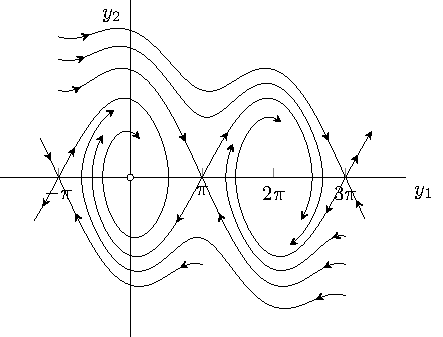
\includegraphics{figSystemPendulumLossyA}
\caption{تقصیری ارتعاش۔مثال \حوالہ{مثال_نظام_دھاگے_سے_لٹکی_کمیت_تقصیری}}
\label{شکل_مثال_نظام_دھاگے_سے_لٹکی_کمیت_تقصیری}
\end{figure}

شکل \حوالہ{شکل_مثال_نظام_دھاگے_سے_لٹکی_کمیت_تقصیری} میں نظام \حوالہ{مساوات_نظام_غیر_خطی_ترکیب_تقصیری_الف} کے خط حرکت دکھائے گئے ہیں۔چونکہ قصری نظام میں توانائی کا ضیاع پایا جاتا ہے لہٰذا شکل \حوالہ{شکل_مثال_نظام_دھاگے_سے_لٹکی_کمیت} کے بند دائروں کی بجائے شکل \حوالہ{شکل_مثال_نظام_دھاگے_سے_لٹکی_کمیت_تقصیری} کے مرغولی خطوط حاصل ہوتے ہیں جو ہمارے توقع کے عین مطابق ہے۔مزید یہ کہ دوری لہری خطوط بھی کسی نہ کسی مقام پر نقطہ فاصل کے گرد گھومنا شروع کر دیتے ہیں۔ اس کے علاوہ اب قصری نظام میں نقطہ زین کو ملانے والے خط نہیں پائے جاتے۔
\انتہا{مثال}
%======================
\ابتدا{مثال}\شناخت{مثال_نظام_شکار_شکاری}\quad آبادی شکار اور شکاری۔ [مسئلہ لوٹکا-ولٹیرا]\\
یہاں لومڑی (شکاری) اور خرگوش (شکار) کی آبادی کے مسئلے پر غور کرتے ہیں۔

\موٹا{پہلا قدم}: ہم فرض کرتے ہیں کہ خرگوش کو جتنی خوراک چاہیے دستیاب ہے۔ یوں لومڑی کی غیر موجودگی میں ان کی تعداد \عددی{y_1'=ay_1} کے تحت قوت نمائی طور پر بڑھے گی۔ لومڑی کی موجودگی میں (اتفاقی آمنے سامنے سے)  خرگوش کی تعداد میں \عددی{y_1y_2} کے راست متناسب کمی پیدا ہو گی۔یوں خرگوش کی تعداد \عددی{y_1'=ay_1-by_1y_2} سے حاصل ہو گی جہاں مستقل \عددی{a>0} اور \عددی{b>0} ہیں۔اسی طرح خرگوش کی غیر موجودگی میں لومڑی کی تعداد \عددی{y_2'=-ly_2} کے تحت قوت نمائی طور پر گھٹے گی۔خرگوش کی موجودگی میں (اتفاقی آمنے سامنے سے) لومڑی کی تعداد \عددی{y_1y_2} کے راست متناسب بڑھے گی۔یوں خرگوش کی موجودگی میں  \عددی{y_2'=-ly_2+ky_1y_2} لومڑی کی تعداد دے گا جہاں مستقل \عددی{l>0} اور \عددی{k>0} ہیں۔

یوں غیر خطی \اصطلاح{مسئلہ لوٹکا-ولٹیرا}\حاشیہد{امریکی ماہر حیاتی طبیعیات الفرڈ جیمز لوٹکا [1880-1949] اور اطالوی ریاضی دان ویٹو ولٹیرا [1860-1940] نے شکار اور شکاری کے مسئلے کو پیش کیا۔} 
\begin{gather}\label{مثال_نظام_شکار_شکاری_الف}
\begin{aligned}
y_1'&=f_1(y_1,y_2)=ay_1-by_1y_2\\
y_2'&=f_2(y_1,y_2)=ky_1y_2-ly_2
\end{aligned}
\end{gather}
حاصل ہوتا ہے۔

\موٹا{دوسرا قدم} مسئلے کو خطی بنانا اور نقطہ فاصل \عددی{(0,0)} کا حصول  ہے۔مساوات \حوالہ{مثال_نظام_شکار_شکاری_الف} کو دیکھ کر نقطہ فاصل مساوات 
\begin{align}
f_1(y_1,y_2)=y_1(a-by_2)=0, \quad f_2(y_1,y_2)=y_2(ky_1-l)=0
\end{align}
کے حل سے \عددی{(y_1,y_2)=(0,0)} اور \عددی{(\tfrac{l}{k},\tfrac{a}{b})} حاصل ہوتے ہیں۔آئیں \عددی{(0,0)} پر غور کریں۔ نقطہ \عددی{(0,0)} کے ہمسائیگی میں مساوات \حوالہ{مثال_نظام_شکار_شکاری_الف} میں \عددی{-by_1y_2} اور \عددی{ky_1y_2} کو نظر انداز کرتے ہوئے خطی نظام
\begin{align*}
\bM{y}'=\begin{bmatrix*}[r] a&0\\0&-l \end{bmatrix*}\bM{y}
\end{align*}
حاصل ہوتا ہے جس کی آئگنی قدر \عددی{\lambda_1=a>0} اور \عددی{\lambda_2=-l<0} کی علامتیں آپس میں الٹ ہیں لہٰذا \عددی{(0,0)} پر نقطہ زین پایا جاتا ہے۔

\موٹا{تیسرا قدم} مسئلے کو خطی بنانا اور نقطہ فاصل \عددی{(\tfrac{l}{k},\tfrac{a}{b})} کا حصول  ہے۔دوسرا نقطہ فاصل \عددی{(y_1,y_2)=(\tfrac{l}{k},\tfrac{a}{b})} پر پایا جاتا ہے۔اس نقطے  کو \عددی{(0,0)} منتقل کرنے کی خاطر ہم \عددی{y_1=\tilde{y}_1+\tfrac{l}{k}} اور \عددی{y_2=\tilde{y}_2+\tfrac{a}{b}} چنتے ہیں۔یوں نقطہ فاصل \عددی{(\tilde{y}_1,\tilde{y}_2)=(0,0)} لکھا جا سکتا ہے۔ چونکہ \عددی{y_1=\tilde{y}_1'} اور \عددی{y_2'=\tilde{y}_2'} ہیں لہٰذا نظام \حوالہ{مثال_نظام_شکار_شکاری_الف} کو درج ذیل لکھا جا سکتا ہے۔
\begin{align*}
\tilde{y}_1'&=\left(\tilde{y}_1+\frac{l}{k}\right)\left[a-b\left(\tilde{y}_2+\frac{a}{b}\right)\right]=\left(\tilde{y}_1+\frac{l}{k}\right)(-b\tilde{y}_2)\\
\tilde{y}_2'&=\left(\tilde{y}_2+\frac{a}{b}\right)\left[k\left(\tilde{y}_1+\frac{l}{k}\right)-l\right]=\left(\tilde{y}_2+\frac{a}{b}\right)k\tilde{y}_1
\end{align*}
نقطہ \عددی{(\tilde{y}_1,\tilde{y}_2)=(0,0)} کے ہمسائیگی میں \عددی{-b\tilde{y}_1\tilde{y}_2} اور \عددی{k\tilde{y}_1\tilde{y}_2} کو نظر انداز کرتے ہوئے خطی نظام
\begin{gather}\label{مثال_نظام_شکار_شکاری_ب}
\begin{aligned}
\tilde{y}_1'&=-\frac{bl}{k}\tilde{y}_2\quad \quad \text{(الف)}\\
\tilde{y}_2'&=\frac{ak}{b}\tilde{y}_1\quad \quad \text{(ب)}
\end{aligned}
\end{gather}
حاصل ہوتا ہے۔مساوات \حوالہ{مثال_نظام_شکار_شکاری_ب}-الف کا بایاں ہاتھ ضرب مساوات-ب کا دایاں ہاتھ برابر ہو گا الف کا دایاں ضرب ب کا بایاں،
\begin{align*}
\frac{ak}{b}\tilde{y}_1'\tilde{y}_1=-\frac{bl}{k}\tilde{y}_2'\tilde{y}_2 \implies \frac{ak}{b}\tilde{y}_1^2+\frac{bl}{k}\tilde{y}_2^2=C
\end{align*}
جس کا تکمل لیتے ہوئے \عددی{\tilde{y}_1} بالمقابل \عددی{\tilde{y}_2} کا \اصطلاح{ترخیمی}\فرہنگ{ترخیم}\حاشیہب{elliptic}\فرہنگ{elliptic} تعلق حاصل کیا گیا ہے۔یوں \عددی{(\tfrac{l}{k},\tfrac{a}{b})} پر شکل \حوالہ{شکل_مثال_نظام_شکار_شکاری} میں دکھایا گیا \اصطلاح{وسط} پایا جاتا ہے۔
\begin{figure}
\centering
\begin{tikzpicture}
%axis
\draw(0,0)--++(4,0)node[right]{$y_1$};
\draw(0,0)--++(0,2)node[left]{$y_2$};
\draw[->-=0.25] ([shift={(0:1cm and 0.5cm)}]2,1) arc  (0:180:1cm and 0.5cm) arc (-180:0:1cm and 0.5cm);
\draw[fill=white](2,1) node[ocirc](kc){};
\draw[dashed] (kc)--(0,1)node[left]{$\frac{a}{b}$};
\draw[dashed](kc)--(2,0)node[below]{$\frac{l}{k}$};
\end{tikzpicture}
\caption{شکار اور شکاری کی آبادی: ماحولیاتی توازن۔}
\label{شکل_مثال_نظام_شکار_شکاری}
\end{figure}

نسبتاً مشکل تجزیے سے ثابت کیا جا سکتا ہے کہ غیر خطی نظام \حوالہ{مثال_نظام_شکار_شکاری_الف} کا \عددی{(\tfrac{l}{k},\tfrac{a}{b})}  پر وسط پایا جاتا ہے البتہ خط حرکت اس نقطے کے گرد غیر ترخیمی بند دائرہ بناتا ہے۔

شکل \حوالہ{شکل_مثال_نظام_شکار_شکاری} کے دائیں کنارے پر خرگوش کی تعداد \عددی{y_1} زیادہ سے زیادہ ہے جس کی وجہ سے لومٹری کی تعداد \عددی{y_2} میں اضافے کی شرح بھی زیادہ سے زیادہ ہے۔اس خط پر گھڑی کی الٹی سمت چلتے ہوئے لومڑی کی زیادہ سے زیادہ آبادی حاصل ہوتی ہے۔اس مقام پر خرگوش کی تعداد اتنی کم ہو چکی ہوتی ہے کہ لومڑی کی بڑھتی تعداد کو خوراک پورا نہیں ہو پایا لہٰذا لومڑی کی آبادی گھٹنے شروع ہو جاتی ہے۔آپ دیکھ سکتے ہیں کہ دونوں جانوروں کی دوری تعداد حالات کے مطابق مسلسل تبدیل ہوتی ہے۔

شکار اور شکاری کی دیگر مثالیں ملخ اور گھاس، ببر شیر اور زیبرا ہیں۔
\انتہا{مثال}
%=====================


\جزوحصہ{سطح حرکت پر ایک درجی مساوات میں تبادلہ}
سطح حرکت کی دوسری ترکیب خود مختار [جس میں \عددیء{t} صریحاً نہیں پایا جاتا] دو درجی سادہ تفرقی مساوات
\begin{align*}
F(y,y',y'')=0
\end{align*}
میں \عددی{y=y_1} کو آزاد متغیرہ اور \عددی{y'=y_2} لے کر \عددی{y''} کو زنجیری تفرق سے
\begin{align*}
y''=y_2'=\frac{\dif y_2}{\dif t}=\frac{\dif y_2}{\dif y_1}\frac{\dif y_1}{\dif t}=\frac{\dif y_2}{\dif y_1}y_2
\end{align*}
لکھ کر ایک درجی مساوات
\begin{align}
F\left(y_1,y_2,\frac{\dif y_2}{\dif y_1}y_2\right)=0
\end{align}
میں تبدیل کرنے پر مبنی ہے۔اس ایک درجی مساوات کو یا تو حل کرنا ممکن ہوتا ہے اور یا \اصطلاح{میدان ڈھال}\فرہنگ{میدان!ڈھال}\فرہنگ{ڈھال!میدان} کی مدد سے اس پر غور ممکن ہوتا ہے۔ آئیں مثال \حوالہ{مثال_نظام_دھاگے_سے_لٹکی_کمیت} پر اس ترکیب کی مدد سے غور کریں۔
%==========

\ابتدا{مثال}\شناخت{مثال_نظام_بلا_تقصیر_ارتعاش_یک_درجی_مساوات}\quad بلا تقصیر ارتعاشی نظام کی ایک درجی تفرقی مساوات۔\\
مساوات \حوالہ{مساوات_نظام_غیر_خطی_ترکیب_مرحلہ_ت} میں \عددی{\theta''+k\sin \theta=0} ہے جس میں \عددی{\theta=y_1} اور  \عددی{\theta'=y_2} (زاویائی رفتار) لیتے ہوئے
\begin{align*}
\theta''=\frac{\dif y_2}{\dif t}=\frac{\dif y_2}{\dif y_1}\frac{\dif y_1}{\dif t}=\frac{\dif y_2}{\dif y_1}y_2
\end{align*}
لکھ کر \عددی{\tfrac{\dif y_2}{\dif y_1}y_2=-k\sin y_1} ملتا ہے جس کو علیحدگی متغیرات سے \عددی{y_2\dif y_2=-k\sin y_1\dif y_1} لکھا جا سکتا ہے جس کا تکمل
\begin{align}\label{مساوات_نظام_کل_توانائی_الف}
\frac{1}{2}y_2^2=k\cos y_1+C 
\end{align}
دیتا ہے جہاں \عددی{C} تکمل کا مستقل ہے۔اس کو \عددی{mL^2} سے ضرب دینے سے
\begin{align*}
\frac{1}{2}m(Ly_2)^2-mL^2k\cos y_1=mL^2C
\end{align*}
حاصل ہوتا ہے جس کے تینوں اجزاء \اصطلاح{توانائی}\فرہنگ{توانائی}\حاشیہب{energy}\فرہنگ{energy} کو ظاہر کرتے ہیں۔چونکہ \عددی{y_2} زاویائی رفتار ہے لہٰذا \عددی{Ly_2} لمحاتی رفتار اور  \عددی{\tfrac{1}{2}m(Ly_2)^2} \اصطلاح{حرکی توانائی}\فرہنگ{حرکی توانائی}\فرہنگ{توانائی!حرکی}\حاشیہب{kinetic energy}\فرہنگ{energy!kinetic} ہے۔درج بالا مساوات کا دوسرا جزو (بمع منفی علامت) \اصطلاح{مخفی توانائی}\فرہنگ{توانائی!مخفی}\فرہنگ{مخفی توانائی}\حاشیہب{potential energy}\فرہنگ{energy!potential} ہے جبکہ مساوات کا دایاں ہاتھ \عددی{mL^2C} کل توانائی ہے۔بلا تقصیر نظام میں توانائی کا ضیاع نہیں پایا جاتا لہٰذا حزب توقع کل توانائی مستقل مقدار ہے۔آئیں دیکھیں کہ حرکت کی نوعیت کل توانائی پر کیسے منحصر ہے۔

شکل \حوالہ{شکل_مثال_نظام_دھاگے_سے_لٹکی_کمیت}-ب مختلف \عددی{C} کے لئے خط حرکت دیتی ہے۔ان خطوط کا دوری عرصہ \عددی{2\pi} ہے۔ان میں ترخیمی بند دائرے اور  لہر نما خطوط شامل ہیں جن کے مابین نقطہ زین [\عددی{(n\pi,0)} جہاں \عددی{n=\mp1,\mp3,\cdots} ہے] سے گزرتے ہوئے دو عدد خط حرکت  پائے جاتے ہیں۔مساوات \حوالہ{مساوات_نظام_کل_توانائی_الف} کے تحت \عددی{C} کی کم سے کم قیمت \عددی{C=-k} ہے جس پر \عددی{y_2=0} اور \عددی{\cos y_1=1} ہوں گے جو ساکن کمیت کو ظاہر کرتی ہے۔جس نقطے پر \عددی{y_2=\theta'=0} ہو اس نقطے پر حرت کی سمت تبدیل ہو کر الٹ ہو جائے گی لہٰذا مساوات \حوالہ{مساوات_نظام_کل_توانائی_الف} میں \عددی{y_2=0} پر کرتے ہوئے \عددی{k\cos y_1+C=0} حاصل ہوتا ہے۔اب اگر \عددی{y_1=\pi} ہو تب \عددی{\cos y_1=-1} اور یوں \عددی{C=k} ہو گا۔اس طرح اگر \عددی{-k<C<k} ہو تب \عددی{\abs{y_1}=\abs{\theta}<\pi} کی صورت میں کمیت کی حرکت کی سمت الٹ ہو گی اور \عددی{C} کی ان قیمتوں \عددی{(\abs{C}<k)} کے لئے کمیت ارتیاش پذیر ہو گا۔ترخیمی بند دائرے اس ارتعاشی حرکت کو ظاہر کرتے ہیں۔اس کے برعکس \عددی{C>k} کی صورت میں \عددی{y_2=0} ممکن نہیں ہے لہٰذا کمیت کی حرکت کی سمت الٹ نہیں ہو گی لہٰذا کمیت مرکز کے گرد گھومتا رہے گا جس کو لہری خط حرکت ظاہر کرتی ہیں۔ان دو صورتوں کے مابین \عددی{C=k} پایا جاتا ہے جس کے خطوط نقطہ زین  سے گزرتے ہیں۔انہیں شکل \حوالہ{شکل_مثال_نظام_دھاگے_سے_لٹکی_کمیت}-ب  میں دکھایا گیا ہے۔
\انتہا{مثال}
%=================== 

دو درجی مساوات کے تبادلے سے سطح حرکت پر (مثال \حوالہ{مثال_نظام_بلا_تقصیر_ارتعاش_یک_درجی_مساوات} کی طرح) قابل حل ایک درجی مساوات کے علاوہ نا قابل حل مساوات بھی اہمیت کے حامل ہے۔ایسی صورت میں میدان ڈھال [حصہ \حوالہ{حصہ_سادہ_ایک_درجی_ڈھال} دیکھیں۔] کے ذریعہ نظام کے بارے میں معلومات حاصل کرنا ممکن ہوتا ہے۔اس عمل کو ایک مشہور مثال کی مدد سے دیکھتے ہیں۔

%===============
\ابتدا{مثال}\quad منحصر بہ خود ارتعاش۔ مساوات ون در پول\\
ایسی طبعی نظام پائے جاتے ہیں جن میں معمولی ارتعاش کی صورت میں نظام کو توانائی فراہم ہوتی ہے جبکہ وسیع ارتعاش کی صورت میں نظام سے توانائی کا اخراج ہوتا ہے۔یوں وسیع ارتعاش کی صورت میں نظام قصری صورت اختیار کرتا ہے جبکہ کم ارتعاش کی صورت میں نظام میں \ترچھا{منفی تقصیر} (نظام کو توانائی کی فراہمی) پائی جاتی ہے۔ ہم طبعی وجوہات کی بنا توقع کرتے ہیں کہ ایسا نظام دوری طرز عمل رکھے گا، جو سطح حرکت پر بند دائرے کی صورت اختیار کرے گا جسے  \اصطلاح{تحدیدی دائرہ}\فرہنگ{تحدیدی دائرہ}\حاشیہب{limit cycle}\فرہنگ{limit cycle} کہتے ہیں۔ایسی ارتعاش کو \اصطلاح{مساوات ون در پول}\فرہنگ{مساوات!ون در پول}\فرہنگ{ون در پول مساوات}\حاشیہب{van del Pol equation}\فرہنگ{van der Pol equation} 
\begin{align}\label{مساوات_نظام_ون_در_پول}
y''-\mu(1-y^2)y'+y=0\quad \quad (\mu >0)
\end{align}
ظاہر کرتی ہے جہاں \عددی{\mu} مثبت مستقل ہے۔یہ مساوات پہلی مرتبہ \اصطلاح{خلا نلکی}\فرہنگ{خلا نلکی}\حاشیہب{vacuum tube}\فرہنگ{vacuum tube} والے برقی ادوار پر غور کے دوران رو پذیر ہوئی۔یہ مساوات \عددی{\mu=0} کی صورت میں ہارمونی ارتعاش کی تفرقی مساوات \عددی{y''+y=0} ہے۔ون در پول مساوات میں قصری جزو \عددی{-\mu(1-y^2)} ہے جہاں \عددی{\mu>0} ہے۔ یوں \عددی{y^2<1} کی صورت میں منفی تقصیری، \عددی{y^2=1} کی صورت میں بلا تقصیر جبکہ \عددی{y^2>1} کی صورت میں مثبت تقصیری (جس میں توانائی کا ضیاع ہو گا) نظام پایا جائے گا۔ نہایت کم \عددی{\mu} کی صورت میں مساوات ون در پول اور \عددی{y''+y=0} میں بہت کم فرق پایا جائے گا لہٰذا ہم توقع کرتے ہیں کہ سطح حرکت پر تحدیدی دائرہ تقریباً گول دائرہ ہو گا۔اگر \عددی{\mu} کی قیمت زیادہ ہو تب تحدیدی دائرہ کی شکل غالباً مختلف ہو گی۔

اس مساوات کو ایک درجی مساوات میں تبدیل کرنے کی خاطر \عددی{y=y_1}، \عددی{y'=y_2} اور \عددی{y''=\tfrac{\dif y_2}{\dif y_1}y_2} لکھتے ہوئے  ون در پول مساوات درج ذیل صورت اختیار کرتی ہے۔
\begin{align}
\frac{\dif y_2}{\dif y_1}y_2-\mu(1-y_1^2)y_2+y_1=0
\end{align}
سطح حرکت (\عددیء{y_1y_2} سطح) پر \اصطلاح{ہم میلان}\فرہنگ{ہم میلان}\حاشیہب{isoclines}\فرہنگ{isoclines} خط \عددی{\tfrac{\dif y_2}{\dif y_1}=K} ہیں جہاں \عددی{K} مستقل مقدار ہے۔یوں ہم میلان خطوط درج ذیل ہوں گے
\begin{align*}
\frac{\dif y_2}{\dif y_1}=\mu(1-y_1^2)-\frac{y_1}{y_2}=K
\end{align*}
جن سے 
\begin{align}
y_2=\frac{y_1}{\mu(1-y_1^2)-K}\quad \quad \text{(\RL{شکل \حوالہ{شکل_نظام_ون_ڈر_پول_پہلی_شکل} اور شکل \حوالہ{شکل_نظام_ون_ڈر_پول_دوسری_شکل} دیکھیں۔})}
\end{align}
حاصل ہوتا ہے۔
\begin{figure}
\centering
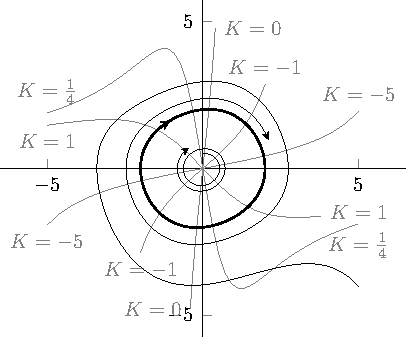
\includegraphics{figSystemVanDerPolEquationA}
\caption{ون ڈر پول مساوات؛ \عددی{\mu=0.1} لیتے ہوئے دو خط حرکت کو تحدیدی دائرہ تک پہنچتے ہوئے دکھایا گیا ہے۔}
\label{شکل_نظام_ون_ڈر_پول_پہلی_شکل}
\end{figure}

شکل \حوالہ{شکل_نظام_ون_ڈر_پول_پہلی_شکل} میں \عددی{\mu} کی کم قیمت \عددی{(\mu=0.1)} کے لئے چند ہم میلان خطوط کو ہلکی سیاہی میں دکھایا گیا ہے۔اس کے علاوہ تحدیدی دائرے کو موٹی لکیر سے ظاہر کیا گیا ہے۔تحدیدی دائرہ تقریباً گول ہے۔ ایک خط حرکت، جو تحدیدی دائرے کے باہر ہے، اور دوسرا خط حرکت، جو تحدیدی دائرے کے اندر  ہے، کو  تحدیدی دائرے تک پہنچتے ہوئے دکھایا گیا ہے۔تحدیدی دائرہ اور نقطہ فاصل کے گرد بند دائرہ (وسط) میں فرق یہ ہے کہ تحدیدی دائرے تک خط حرکت پہنچتی ہے جبکہ وسط کا خط اسی دائرے پر پایا جاتا ہے۔ \عددی{\mu} کی زیادہ قیمت پر تحدیدی دائرہ گول صورت نہیں رکھتا۔ شکل \حوالہ{شکل_نظام_ون_ڈر_پول_دوسری_شکل} میں \عددی{\mu} کی زیادہ قیمت \عددی{(\mu=1)} کے لئے  تمام صورت حال دکھائی گئی ہے جہاں تحدیدی دائرہ گول نہیں ہے۔
\begin{figure}
\centering
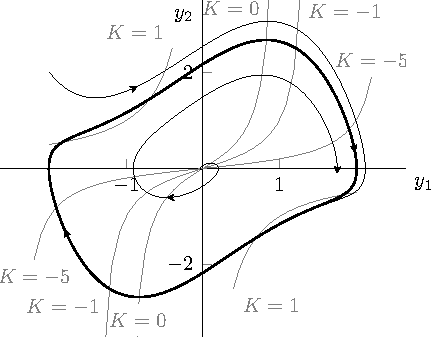
\includegraphics{figSystemVanDerPolEquationB}
\caption{ون ڈر پول مساوات؛ \عددی{\mu=1} لیتے ہوئے دو خط حرکت کو تحدیدی دائرہ تک پہنچتے ہوئے دکھایا گیا ہے۔}
\label{شکل_نظام_ون_ڈر_پول_دوسری_شکل}
\end{figure}
\انتہا{مثال}
%=====================
\ابتدا{مثال}
تفرقی مساوات \عددی{y''+y-y^3=0} سے نظام حاصل کریں۔اس نظام کے تمام نقطہ فاصل دریافت کریں۔نقطہ فاصل کی نوعیت دریافت کریں۔

حل:\عددی{y=y_1} اور \عددی{y'=y_1'=y_2} لیتے ہوئے اور \عددی{y''=y_2'} لکھتے ہوئے دیے گئے دو درجی مساوات سے نظام
\begin{gather}
\begin{aligned}\label{مساوات_مثال_نظام_تفرقی_سے_نظام}
y_1'&=f_1=y_2\\
y_2'&=f_2=-y_1+y_1^3
\end{aligned}
\end{gather}
 حاصل ہوتا ہے۔نقطہ فاصل \عددی{f_1=f_2=0} سے حاصل ہوں گے۔\عددی{f_1=0} سے \عددی{y_2=0} ملتا ہے جبکہ \عددی{f_2=y_1(-1+y_1^2)=0} سے \عددی{y_1=0} اور \عددی{y_1=\mp 1} ملتے ہیں۔یوں نقطہ فاصل \عددی{(0,0)}، \عددی{-1,0} اور \عددی{1,0} ہیں۔نقطہ فاصل \عددی{(0,0)} مرکز پر پایا جاتا ہے لہٰذا اس پر پہلے غور کرتے ہیں۔نقطہ فاصل کی نوعیت جاننے کی خاطر نظام کو خطی بناتے ہیں۔ایسا کوئی بھی جزو جو \عددی{y^m} یا \عددی{y_1^ny_2^q} کی صورت میں لکھا گیا ہو، جہاں \عددی{m \ne 1} جبکہ \عددی{n} اور \عددی{q} کوئی بھی  مستقل ہو سکتے ہیں، غیر خطی ہو گا۔ان غیر خطی اجزاء کو رد کرنے سے خطی نظام حاصل ہوتا ہے۔یوں \عددی{y_2'} کی مساوات میں \عددی{y_1^3} کو رد کرتے ہوئے خطی نظام 
\begin{gather*}
\begin{aligned}
y_1'&=y_2\\
y_2'&=-y_1
\end{aligned}\quad \implies \quad
\begin{aligned}
\bM{y}'=\begin{bmatrix} 0&1\\-1&0 \end{bmatrix}\bM{y}
\end{aligned}
\end{gather*}
حاصل ہو گا جس سے  \عددی{p=a_{11}+a_{22}=0}، \عددی{q=1>0} اور \عددی{\Delta=-4<0} ملتے ہیں لہٰذا نقطہ \عددی{(0,0)} مستحکم وسط ہے۔

آئیں اب نقطہ \عددی{(-1,0)} پر غور کریں۔اس کو مرکز منتقل کرنے کی خاطر نظام \حوالہ{مساوات_مثال_نظام_تفرقی_سے_نظام} میں \عددی{\tilde{y}_1=y_1+1} یعنی \عددی{y_1=\tilde{y}_1-1} اور \عددی{\tilde{y}_2=y_2} پر کرتے ہوئے
\begin{gather*}
\begin{aligned}
\tilde{y}_1'&=\tilde{y}_2\\
\tilde{y}_2'&=-(\tilde{y}_1-1)+(\tilde{y}_1-1)^3
\end{aligned}\implies
\begin{aligned}
\tilde{y}_1'&=\tilde{y}_2\\
\tilde{y}_2'&=2\tilde{y}_1-3\tilde{y}_1^2+\tilde{y}_1^3
\end{aligned}
\end{gather*}
ملتا ہے۔ غیر خطی اجزاء \عددی{\tilde{y}_1^2} اور \عددی{\tilde{y}_1^3} کو رد کرتے ہوئے خطی نظام
\begin{gather*}
\begin{aligned}
\tilde{y}_1'&=\tilde{y}_2\\
\tilde{y}_2'&=2\tilde{y}_1
\end{aligned}\implies 
\begin{aligned}
\tilde{\bM{y}}'=\begin{bmatrix}0&1\\2&0  \end{bmatrix}\tilde{\bM{y}}
\end{aligned}
\end{gather*}
ملتا ہے۔اس سے \عددی{p=0}، \عددی{q=-2<0} اور \عددی{\Delta=8>0} حاصل ہوتے ہیں لہٰذا نقطہ \عددی{(-1,0)} غیر مستحکم نقطہ زین ہے۔

نقطہ \عددی{(1,0)} پر غور کرنے کی  خاطر اس کو مرکز منتقل کرتے ہیں۔ایسا کرنے کی خاطر \عددی{\tilde{y}_1=y_1-1} اور \عددی{\tilde{y}_2=y_2} چنتے ہیں۔یوں نظام
\begin{align*}
\tilde{y}_1'&=\tilde{y}_2\\
\tilde{y}_2'&=2\tilde{y}_1+3\tilde{y}_1^2+\tilde{y}_1^3
\end{align*}
ملتا ہے جس میں غیر خطی اجزاء  \عددی{\tilde{y}_1^2} اور \عددی{\tilde{y}_1^3} رد کرتے ہوئے  خطی نظام
\begin{gather*}
\begin{aligned}
\tilde{y}_1'&=\tilde{y}_2\\
\tilde{y}_2'&=2\tilde{y}_1
\end{aligned}\implies 
\begin{aligned}
\tilde{\bM{y}}'=\begin{bmatrix}0&1\\2&0  \end{bmatrix}\tilde{\bM{y}}
\end{aligned}
\end{gather*}

ملتا ہے۔اس سے \عددی{p=0}، \عددی{q=-2<0} اور \عددی{\Delta=8>0} حاصل ہوتے ہیں لہٰذا نقطہ \عددی{(1,0)} غیر مستحکم نقطہ زین ہے۔
\انتہا{مثال}
%======================

\حصہء{سوالات}
سوال \حوالہ{سوال_نظام_خطی_بنانا_الف} تا سوال \حوالہ{سوال_نظام_خطی_بنانا_ب} کو \موٹا{خطی بناتے} ہوئے تمام نقطہ فاصل دریافت کریں۔ نقطہ فاصل کی نوعیت جدول \حوالہ{جدول_نظام_نقطہ_فاصل_اصول_جانچ} اور جدول \حوالہ{جدول_نظام_نقطہ_فاصل_بالمقابل_استحکام} کی مدد سے دریافت کریں۔

%===============
\ابتدا{سوال}\شناخت{سوال_نظام_خطی_بنانا_الف}\quad 
$y_1'=4y_1-y_1^2,\quad y_2'=y_2$

جوابات:نقطہ فاصل \عددی{f_1=f_2=0} سے \عددی{(0,0)} اور \عددی{(4,0)} حاصل ہوتے ہیں۔مسئلے کو \عددی{(0,0)} پر خطی بناتے ہوئے \عددی{\bM{A}=\begin{bmatrix} 4&0\\0&1  \end{bmatrix}} لکھا جاتا ہے جس سے \عددی{p>0}، \عددی{q>0} اور \عددی{\Delta>0} ملتا ہے لہٰذا نقطہ \عددی{(0,0)} غیر مستحکم جوڑ ہے۔ نقطہ \عددی{(4,0)} کو مرکز پر منتقل کرنے کی خاطر \عددی{\tilde{y}_1=y_1-4} اور \عددی{\tilde{y}_2=y_2} پر کرتے ہیں اور مسئلے کو (\عددی{-\tilde{y}_1^2} رد کرتے ہوئے) خطی بناتے ہوئے \عددی{\bM{A}=\begin{bmatrix} -4&0\\0&1  \end{bmatrix}} حاصل ہوتا ہے جو \عددی{p<0}، \عددی{q<0} اور \عددی{\Delta>0} دیتا ہے  جو غیر مستحکم نقطہ زین کو ظاہر کرتی ہے۔
\انتہا{سوال}
%======================
\ابتدا{سوال}\quad 
$y_1'=y_2,\quad y_2'=-y_1+\frac{2}{3}y_1^2$\\
جوابات:نقطہ فاصل \عددی{f_1=f_2=0} سے \عددی{(0,0)} اور \عددی{(\tfrac{3}{2},0)} حاصل ہوتے ہیں۔نقطہ \عددی{(0,0)} پر مسئلہ خطی بناتے ہوئے \عددی{\bM{A}=\begin{bmatrix} 0&1\\-1&0  \end{bmatrix}} حاصل ہوتا ہے جس سے \عددی{p=0}، \عددی{q>0} اور \عددی{\Delta<0} ملتے ہیں لہٰذا نقطہ \عددی{(0,0)} مستحکم وسط ہے۔ نقطہ \عددی{(\tfrac{3}{2},0)} کو مرکز پر منتقل کرنے کی خاطر \عددی{\tilde{y}_1=y_1-\tfrac{3}{2}} اور \عددی{\tilde{y}_2=y_2} پر کرتے ہیں اور  مسئلے کو (\عددی{\tfrac{2}{3}\tilde{y}_1^2} رد کرتے ہوئے) خطی بنانے سے  \عددی{\bM{A}=\begin{bmatrix} 0&1\\1&0  \end{bmatrix}} حاصل ہوتا ہے لہٰذا \عددی{(\tfrac{2}{3},0)} غیر مستحکم نقطہ زین ہے۔
\انتہا{سوال}
%======================
\ابتدا{سوال}\quad 
$y_1'=y_2,\quad y_2'=-2y_1-y_1^2$\\
جوابات:مستحکم وسط \عددی{(0,0)} پر پایا جاتا ہے جبکہ \عددی{(-2,0)} غیر مستحکم نقطہ زین  ہے۔
\انتہا{سوال}
%======================
\ابتدا{سوال}\quad 
$y_1'=-y_1+y_2+y_1^2,\quad y_2'=-y_1-y_2$\\
جوابات:\عددی{(0,0)} پر مستحکم اور جاذب نقطہ مرغولہ پایا جاتا ہے جبکہ \عددی{(-2,2)} پر غیر مستحکم نقطہ زین پایا جاتا ہے۔
\انتہا{سوال}
%======================
\ابتدا{سوال}\شناخت{سوال_نظام_خطی_بنانا_ب}\quad 
$y_1'=-y_1+y_2-y_2^2,\quad y_2'=-y_1-y_2$\\
جوابات:\عددی{(0,0)} پر جاذب  نقطہ مرغولہ  پایا جاتا ہے جبکہ \عددی{(-2,2)} پر غیر مستحکم نقطہ زین پایا جاتا ہے۔
\انتہا{سوال}
%======================

سوال \حوالہ{سوال_نظام_تفرقی_سے_نظام_الف} تا سوال \حوالہ{سوال_نظام_تفرقی_سے_نظام_ب} میں تفرقی مساوات سے نظام حاصل کریں۔اس نظام کے تمام نقطہ فاصل دریافت کریں۔نظام کو خطی بناتے ہوئے نقطہ فاصل کی نوعیت دریافت کریں۔

%==================
\ابتدا{سوال}\شناخت{سوال_نظام_تفرقی_سے_نظام_الف}\quad 
$y''-4y+y^3=0$\\
جوابات: نظام \عددی{y_1'=y_2} اور \عددی{y_2'=4y_1-y_1^3} حاصل ہوتا ہے۔\عددی{(0,0)} غیر مستحکم نقطہ زین، \عددی{(-2,0)} مستحکم وسط اور \عددی{(2,0)} مستحکم وسط ہیں۔
\انتہا{سوال}
%========================
\ابتدا{سوال}\quad 
$y''+4y-y^3=0$\\
جوابات: نظام \عددی{y_1'=y_2} اور \عددی{y_2'=4y_1-y_1^3} حاصل ہوتا ہے۔\عددی{(0,0)} مستحکم وسط، \عددی{(-2,0)} غیر مستحکم نقطہ زین اور \عددی{(2,0)} غیر مستحکم نقطہ زین ہیں۔
\انتہا{سوال}
%========================
\ابتدا{سوال}\quad 
$y''+4y+y^2=0$\\
جوابات:\عددی{(0,0)} مستحکم وسط اور \عددی{(-4,0)} غیر مستحکم نقطہ زین ہے۔
\انتہا{سوال}
%========================
\ابتدا{سوال}\quad 
$y''+\sin y=0$\\
جوابات: \عددی{(0,0)} اور \عددی{(\mp n2\pi,0)} مستحکم وسط ہیں جہاں \عددی{n=1,2,3,\cdots} ہو سکتا ہے۔نقطہ \عددی{(\mp m\pi,0)} غیر مستحکم نقطہ زین ہے جہاں \عددی{m=1,3,5,\cdots} ہو سکتا ہے۔
\انتہا{سوال}
%========================
\ابتدا{سوال}\شناخت{سوال_نظام_تفرقی_سے_نظام_ب}\quad 
$y''+\cos y=0$\\
جوابات: نقطہ \عددی{(\tfrac{\pi}{2}\mp n2\pi,0)} غیر مستحکم نقطہ نیز  جبکہ \عددی{(-\tfrac{\pi}{2}\mp n2\pi,0)} وسط ہیں جہاں \عددی{n=1,2,3,\cdots} ہو سکتا ہے۔آپ کو \عددی{-\cos(\mp\tfrac{\pi}{2}+\tilde{y}_1)=\sin(\mp \tilde{y}_1)\approx \mp \tilde{y}_1} کی مدد لے سکتے ہیں۔
\انتہا{سوال}
%========================
\ابتدا{سوال}\quad ریلے مساوات\\
\عددی{Y''-\mu(1-\tfrac{1}{3}Y'^2)Y'+Y=0} جہاں \عددی{\mu >0} ہے، \اصطلاح{ریلے مساوات}\فرہنگ{ریلے مساوات}\فرہنگ{مساوات!ریلے}\حاشیہب{Rayleigh equation}\فرہنگ{Rayleigh equation}\فرہنگ{equation!Rayleigh}  کہلاتی\حاشیہد{لارڈ ریلے، جن کا اصل نام جان ولیم سٹرٹ ہے  انگلستان کے ماہر طبیعیات اور ریاضی دان تھے۔} ہے۔اس میں \عددی{y=Y'} پر کرتے ہوئے تفرق لے کر \موٹا{ون در پول مساوات} حاصل کریں۔
\انتہا{سوال}
%====================
\ابتدا{سوال}\quad ڈفنگ مساوات\\
اسپرنگ اور کمیت کی مساوات \عددی{y''+\omega_0^2=0} میں غیر خطی قوت بحالی کی صورت میں \اصطلاح{ڈفنگ مساوات}\فرہنگ{ڈفنگ مساوات}\فرہنگ{مساوات!ڈفنگ}\حاشیہب{Duffing equation}\فرہنگ{equation!Duffing}\فرہنگ{Duffing equation} \عددی{y''+\omega_0^2y+\beta y^3=0} حاصل ہوتی ہے جہاں \عددی{\abs{\beta}} عموماً چھوٹی مقدار ہوتی ہے۔\عددی{\beta>0} کو \ترچھا{سخت اسپرنگ} اور \عددی{\beta<0} کو \ترچھا{نرم اسپرنگ} کی صورت پکارا جاتا ہے۔سطح حرکت پر خط حرکت کی مساوات دریافت کریں۔

جواب:\عددی{2y_2^2+2\omega_0^2y_1^2+\beta y_1^4=K} جہاں \عددی{K} مستقل مقدار ہے۔
\انتہا{سوال}
%====================
\ابتدا{سوال}\quad خط حرکت\\
سادہ تفرقی مساوات \عددی{y''-9y+y^3=0} کو نظام کی صورت میں لکھیں جس کو حل کرتے ہوئے \عددی{y_2} بالمقابل \عددی{y_1} کی مساوات حاصل کریں۔حاصل مساوات سے سطح حرکت پر چند خط حرکت کھینچیں۔

جواب:\عددی{2y_2^2=18y_1^2-y_1^4+K} جہاں \عددی{K} مستقل مقدار ہے۔
\انتہا{سوال}
%=====================

\حصہ{سادہ تفرقی مساوات کے غیر متجانس خطی نظام}
اس حصے میں غیر متجانس نظام
\begin{align}\label{مساوات_نظام_غیر_متجانس_مساوات_الف}
\bM{y}'=\bM{A}\bM{y}+\bM{g}\quad \quad \text{\RL{(حصہ \حوالہ{حصہ_نظام_نظریہ_نظام} دیکھیں)}}
\end{align}
جہاں \عددی{\bM{g}} غیر صفر سمتیہ  ہے، کو حل کرنا سیکھتے ہیں۔ہم فرض کرتے ہیں کہ \عددی{\bM{g}(t)} اور \عددی{n \times n} قالب \عددی{\bM{A}(t)} کے ارکان،  محور \عددی{t} کے کھلے وقفہ \عددی{J} پر استمراری ہیں۔وقفہ \عددی{J} پر متجانس مساوات \عددی{\bM{y}'=\bM{A}\bM{y}} کے عمومی حل \عددی{\bM{y}^{(h)}(t)} اور \عددی{J} پر مساوات \حوالہ{مساوات_نظام_غیر_متجانس_مساوات_الف} کے کسی بھی \اصطلاح{مخصوص حل}\فرہنگ{مخصوص حل}\فرہنگ{particular solution} \عددی{\bM{y}^{(p)}(t)} [جس میں کوئی مستقل نہیں پایا جاتا] سے مساوات \حوالہ{مساوات_نظام_غیر_متجانس_مساوات_الف} کا \عددی{J} پر \اصطلاح{عمومی حل}\فرہنگ{عمومی حل}\فرہنگ{حل!عمومی}\فرہنگ{general!solution}
\begin{align}\label{مساوات_نظام_غیر_متجانس_مساوات_ب}
\bM{y}=\bM{y}^{(h)}+\bM{y}^{(p)}
\end{align}
حاصل ہوتا ہے۔مسئلہ \حوالہ{مسئلہ_نظام_خطی_نظام_وجودیت_یکتائی} کے تحت عمومی حل \عددی{\bM{y}} میں \عددی{J} پر مساوات \حوالہ{مساوات_نظام_غیر_متجانس_مساوات_الف} کے تمام ممکنہ حل شامل ہیں۔

متجانس مساوات کے حل پر ہم گزشتہ حصوں میں غور کر چکے ہیں۔اس حصے میں غیر متجانس مساوات کے مخصوص حل کے حصول پر غور کرتے ہیں۔نا معلوم عددی سر کی ترکیب اور مقدار معلوم بدلنے کے طریقوں پر غور کرتے ہیں جنہیں ہم حصہ \حوالہ{حصہ_سادہ_دو_غیر_متجانس} اور حصہ \حوالہ{سادہ_دو_متغیرات_بدلنے_کا_طریقہ} سے جانتے ہیں۔ 
%=============

\جزوحصہ{نا معلوم عددی سر کی ترکیب}
 ایک عدد سادہ تفرقی مساوات کے حل میں استعمال ہونے کی طرح اب بھی یہ ترکیب اس صورت  قابل استعمال ہو گی جب  \عددی{\bM{A}} کے ارکان مستقل مقدار ہوں  جبکہ مستقل مقدار، \عددی{t^m} (جہاں \عددی{m} مثبت اعداد ہیں)، قوت نمائی، سائن  اور کوسائن تفاعل کا کوئی بھی مجموعہ \عددی{\bM{g}}  ہو۔ایسی صورت میں مخصوص حل کو \عددی{\bM{g}} کی طرح تصور کیا جاتا ہے لہٰذا \عددی{\bM{g}=t^2} ہونے کی صورت میں \عددی{\bM{y}^{(p)}=\bM{u}+\bM{v}t+\bM{w}t^2} فرض کیا جائے گا۔ مساوات \حوالہ{مساوات_نظام_غیر_متجانس_مساوات_الف} میں \عددی{\bM{y}^{(p)}} پر کرتے ہوئے \عددی{\bM{u}}،  \عددی{\bM{v}} اور \عددی{\bM{w}} حاصل کیے جاتے ہیں۔یہ حصہ \حوالہ{حصہ_سادہ_دو_غیر_متجانس} کی طرح ہے البتہ یہاں ترمیمی قاعدہ قدر مختلف ہے۔ آئیں ایک مثال کی مدد سے اس ترکیب کا استعمال دیکھیں۔
%================

\ابتدا{مثال}\شناخت{مثال_نظام_غیر_متجانس_نا_معلوم_سر}\quad نا معلوم عددی سر کی ترکیب۔ترمیمی قاعدہ\\
درج ذیل مساوات کی عمومی حل حاصل کریں۔
\begin{align}\label{مساوات_مثال_غیر_متجانس_نا_معلوم_سر_الف}
\bM{y}'=\bM{A}\bM{y}+\bM{g}=\begin{bmatrix*}[r] -2&1\\1&-2 \end{bmatrix*} \bM{y}+\begin{bmatrix*}[r] -4\\3 \end{bmatrix*} e^{-3t}
\end{align}

حل:ہم صفحہ \حوالہصفحہ{مثال_نظام_خط_حرکت_غیر_مناسب} پر مثال \حوالہ{مثال_نظام_خط_حرکت_غیر_مناسب} میں نظیری متجانس مساوات کا حل 
\begin{align}\label{مساوات_مثال_غیر_متجانس_نا_معلوم_سر_ب}
\bM{y}^{(h)}=c_1\begin{bmatrix} 1 \\ 1 \end{bmatrix}e^{-t}+c_2\begin{bmatrix*}[r] 1\\ -1 \end{bmatrix*}e^{-3t}
\end{align}
حاصل کر چکے ہیں۔چونکہ \عددی{\bM{A}} کا  \عددی{\lambda=-3} آئگنی قدر ہے اور مساوات \حوالہ{مساوات_مثال_غیر_متجانس_نا_معلوم_سر_الف} میں دائیں جانب \عددی{e^{-3t}} پایا جاتا ہے لہٰذا  اس جزو کو \عددی{t} سے ضرب دیتے ہوئے \عددی{\bM{y}^{(p)}} میں شامل کرتے ہیں۔
\begin{align}\label{مساوات_مثال_غیر_متجانس_نا_معلوم_سر_پ}
\bM{y}^{(p)}=\bM{u}te^{-3t}+\bM{v}e^{-3t} \quad \quad 
\end{align} 
\عددی{\bM{y}^{(p)}} میں بائیں ہاتھ کا پہلا جزو حصہ \حوالہ{حصہ_سادہ_دو_غیر_متجانس} کا مماسی  ترمیمی قاعدہ ہے، جو یہاں نا کافی ہے۔[آپ کوشش کر کے دیکھ سکتے ہیں]۔ مساوات \حوالہ{مساوات_مثال_غیر_متجانس_نا_معلوم_سر_پ} کو مساوات \حوالہ{مساوات_مثال_غیر_متجانس_نا_معلوم_سر_الف} میں پر کرتے ہیں۔
\begin{align*}
\bM{y}^{(p)'}=\bM{u}e^{-3t}-3\bM{u}te^{-3t}-3\bM{v}e^{-3t}=\bM{A}\bM{u}te^{-3t}+\bM{A}\bM{v}e^{-3t}+\bM{g}
\end{align*}
دونوں جانب \عددی{te^{-3t}} والے اجزاء کے عددی سر برابر ہوں گے لہٰذا \عددی{-3\bM{u}=\bM{A}\bM{u}} ہو گا۔یوں \عددی{\bM{A}} قالب کے آئگنی قدر \عددی{\lambda=-3} کا نظیری آئگنی سمتیہ \عددی{\bM{u}} ہو گا۔اس طرح \عددی{\bM{u}=a[1\quad -1]^T} لکھا جا سکتا ہے جہاں \عددی{a} کوئی بھی غیر صفر مستقل ہو سکتا ہے۔بقایا اجزاء کے عددی سر برابر لکھ کر
\begin{gather*}
\begin{aligned}
\bM{u}-3\bM{v}=\bM{A}\bM{v}+\bM{g}
\end{aligned}\implies
\begin{aligned}
\begin{bmatrix*}[r] a\\-a  \end{bmatrix*}-\begin{bmatrix} 3v_1\\3v_2 \end{bmatrix}=\begin{bmatrix*}[r] -2v_1+v_2\\v_1-2v_2 \end{bmatrix*}+\begin{bmatrix*}[r] -4\\3 \end{bmatrix*}
\end{aligned} 
\end{gather*}
ترتیب دیتے ہیں۔
\begin{align*}
v_1+v_2&=a+4\\
v_1+v_2&=-a-3
\end{align*}
دوسری مساوات کو پہلی سے منفی کرتے ہوئے \عددی{2a+7=0} یعنی \عددی{a=-\tfrac{7}{2}} ملتا ہے۔یوں درج بالا میں پہلی مساوات \عددی{v_1+v_2=-\tfrac{7}{2}+4=\tfrac{1}{2}} ہو گی جس  میں  \عددی{v_1=k} لیتے ہوئے  \عددی{v_2=\tfrac{1}{2}-k} حاصل ہوتا ہے۔اس طرح \عددی{\bM{v}=[k\quad \tfrac{1}{2}-k]^T} ہو گا۔ہم \عددی{k=0} چن سکتے ہیں۔ایسا ہی کرتے ہوئے عمومی حل لکھتے ہیں۔
\begin{align}
\bM{y}=\bM{y}^{(h)}+\bM{y}^{(p)}=c_1\begin{bmatrix} 1 \\[1em] 1 \end{bmatrix}e^{-t}+c_2\begin{bmatrix*}[r] 1\\[1em] -1 \end{bmatrix*}e^{-3t}-\frac{7}{2}\begin{bmatrix*}[r] 1\\[1em] -1 \end{bmatrix*}te^{-3t}+\begin{bmatrix} 0\\[1em]\frac{1}{2} \end{bmatrix}e^{-3t}
\end{align}
\عددی{k} کی قیمت تبدیل کرتے ہوئے دیگر حل لکھے جا سکتے ہیں مثلاً \عددی{k=1} لیتے ہوئے \عددی{\bM{v}=[1 \quad -\tfrac{1}{2}]^T} حاصل ہو گا جس سے درج ذیل عمومی حل ملتا ہے۔
 \begin{align}
\bM{y}=\bM{y}^{(h)}+\bM{y}^{(p)}=c_1\begin{bmatrix} 1 \\[1em] 1 \end{bmatrix}e^{-t}+c_2\begin{bmatrix*}[r] 1\\[1em] -1 \end{bmatrix*}e^{-3t}-\frac{7}{2}\begin{bmatrix*}[r] 1\\[1em] -1 \end{bmatrix*}te^{-3t}+\begin{bmatrix*}[r] 1\\[1em]-\frac{1}{2} \end{bmatrix*}e^{-3t}
\end{align}
\انتہا{مثال}
%====================
\جزوحصہء\quad مقدار معلوم بدلنے کی ترکیب\\
اس ترکیب سے غیر متجانس نظام
\begin{align}\label{مساوات_نظام_غیر_متجانس_مقدار_معلوم_الف}
\bM{y}'=\bM{A}(t)+\bM{g}(t)
\end{align}
کو حل کیا جا سکتا ہے جہاں \عددی{\bM{A}(t)} متغیر مقدار ہیں اور \عددی{\bM{g}(t)} کوئی بھی تفاعل ہو سکتا ہے۔اگر \عددی{t} محور کے کسی کھلے وقفے \عددی{J} پر  نظیری متجانس نظام کا عمومی حل \عددی{\bM{y}^{(h)}} معلوم ہو تب اس ترکیب کی مدد سے اس وقفے پر نظام \حوالہ{مساوات_نظام_غیر_متجانس_مقدار_معلوم_الف} کا مخصوص حل \عددی{\bM{y}^{(p)}} حاصل کیا جاتا ہے۔آئیں مثال \حوالہ{مثال_نظام_غیر_متجانس_نا_معلوم_سر} کو اس ترکیب سے حل کریں۔
%=================
\ابتدا{مثال}\quad مقدار معلوم بدلنے کے طریقے سے حل\\
گزشتہ مثال کے نظام \حوالہ{مساوات_مثال_غیر_متجانس_نا_معلوم_سر_الف} کو مقدار معلوم بدلنے کی ترکیب سے حل کریں۔
\begin{align}
\bM{y}'=\bM{A}\bM{y}+\bM{g}=\begin{bmatrix*}[r] -2&1\\1&-2 \end{bmatrix*} \bM{y}+\begin{bmatrix*}[r] -4\\3 \end{bmatrix*} e^{-3t}
\end{align}

حل:متجانس مساوات کی آئگنی قدر \عددی{\lambda_1=-1} اور \عددی{\lambda_2=-3} ہیں جن کے بالترتیب نظیری آئگنی سمتیات \عددی{[1 \quad 1]^T} اور \عددی{[1\quad -1]^T} ہیں لہٰذا  اساس \عددی{[e^{-t}\quad e^{-t}]^T}، \عددی{[e^{-3t}\quad -e^{-3t}]^T} ہے جس سے متجانس مساوات کا حل \عددی{\bM{y}^{(h)}} لکھتے ہیں۔
\begin{gather}
\begin{aligned}\label{مساوات_نظام_مقدار_معلوم_وائے}
\bM{y}^{(h)}&=c_1\begin{bmatrix}1\\1 \end{bmatrix}e^{-t}+c_2\begin{bmatrix*}[r]  1\\-1\end{bmatrix*}e^{-3t}=\begin{bmatrix*}[r] e^{-t}&e^{-3t} \\ e^{-t} &-e^{-3t} \end{bmatrix*} \begin{bmatrix} c_1\\c_2 \end{bmatrix}=\bM{Y}(t)\bM{c}
\end{aligned}
\end{gather}
یہاں \عددی{\bM{Y}(t)=[\bM{y}^{(1)} \quad \bM{y}^{(2)}]^T} بنیادی قالب [حصہ \حوالہ{حصہ_نظام_نظریہ_نظام} دیکھیں] ہے ۔ حصہ \حوالہ{سادہ_دو_متغیرات_بدلنے_کا_طریقہ} کی طرح ہم مستقل سمتیہ \عددی{\bM{c}} کی جگہ متغیر سمتیہ \عددی{\bM{u}} پر کرتے ہوئے مخصوص حل \عددی{\bM{y}^{(p)}} لکھتے ہیں۔
\begin{align}
\bM{y}^{(p)}=\bM{Y}(t)\bM{u}(t)
\end{align}
نظام \حوالہ{مساوات_مثال_غیر_متجانس_نا_معلوم_سر_الف} میں \عددی{\bM{y}^{(p)}} پر کرتے ہیں۔
\begin{align}\label{مساوات_نظام_بنیادی_نظام_الف}
\bM{Y}'\bM{u}+\bM{Y}\bM{u}'=\bM{A}\bM{Y}\bM{u}+\bM{g}
\end{align}
اب چونکہ \عددی{\bM{y}^{(1)}} اور \عددی{\bM{y}^{(2)}} متجانس نظام کا حل ہے لہٰذا \عددی{\bM{y}^{(1)'}=\bM{A}\bM{y}^{(1)}} اور
 \عددی{\bM{y}^{(2)'}=\bM{A}\bM{y}^{(2)}} یعنی \عددی{\bM{Y}'=\bM{A}\bM{Y}}ہو گا۔یوں \عددی{\bM{Y}'\bM{u}=\bM{A}\bM{Y}\bM{u}} لکھ کر مساوات \حوالہ{مساوات_نظام_بنیادی_نظام_الف} سے  \عددی{\bM{Y}\bM{u}'=\bM{g}} حاصل ہوتا ہے (اور چونکہ \عددی{\bM{Y}} کا امتیازی مقطع دراصل ورونسکی [حصہ \حوالہ{حصہ_نظام_قالب} دیکھیں] \عددی{W} ہے جو اساس کی صورت میں غیر صفر ہوتا ہے لہٰذا \عددی{\bM{Y}^{-1}} حاصل کیا جا سکتا ہے) لہٰذا درج ذیل لکھا جا سکتا ہے۔
\begin{align}
\bM{u}'=\bM{Y}^{-1}\bM{g}
\end{align}
 معکوس قالب کو مساوات \حوالہ{مساوات_نظام_معکوس_قالب} کی مدد سے حاصل کر کے
\begin{align*}
\bM{Y}^{-1}=\frac{1}{-2e^{-4t}}\begin{bmatrix} -e^{-3t} & -e^{-3t}\\[1em] -e^{-t}& e^{-t} \end{bmatrix}=
\frac{1}{2}\begin{bmatrix} e^{t} & e^{t}\\[1em] e^{3t}& -e^{3t}   \end{bmatrix}
\end{align*}
\عددی{\bM{g}} سے ضرب دیتے ہوئے \عددی{\bM{u}'} لکھتے ہیں۔
\begin{align*}
\bM{u}'=\bM{Y}^{-1}\bM{g}=\frac{1}{2}\begin{bmatrix} e^{t} & e^{t}\\[1em] e^{3t}& -e^{3t}   \end{bmatrix}\begin{bmatrix} -4e^{-3t} \\[1em] 3e^{-3t} \end{bmatrix} =\begin{bmatrix}-\frac{1}{2}e^{-2t}\\[1em] -\frac{7}{2}\end{bmatrix}
\end{align*}
\عددی{\bM{u}} حاصل کرنے کی خاطر تکمل لیتے ہیں۔تفرق کی طرح ہر جزو کا علیحدہ تکمل لیا جاتا ہے۔
\begin{align*}
\bM{u}(t)=\int_{0}^{t}\begin{bmatrix}-\frac{1}{2}e^{-2t}\\[1em] -\frac{7}{2}\end{bmatrix}=\begin{bmatrix} \frac{1}{4}(e^{-2t}-1) \\[1em] -\frac{7}{2}t \end{bmatrix}
\end{align*}
یوں مساوات \حوالہ{مساوات_نظام_مقدار_معلوم_وائے} کی مدد سے درج ذیل لکھا جا سکتا ہے۔
\begin{align*}
\bM{y}^{(p)}=\bM{Y}\bM{u}&=\begin{bmatrix*}[r] e^{-t}&e^{-3t} \\ e^{-t} &-e^{-3t} \end{bmatrix*}\begin{bmatrix} \frac{1}{4}(e^{-2t}-1) \\[1em] -\frac{7}{2}t \end{bmatrix}=\begin{bmatrix}\frac{1}{4}e^{-3t}-\frac{1}{4}e^{-t}-\frac{7}{2}te^{-3t}\\[1em] \frac{1}{4}e^{-3t}-\frac{1}{4}e^{-t}+\frac{7}{2}te^{-3t}  \end{bmatrix}\\
&=\begin{bmatrix} \frac{1}{4}-\frac{7}{2}t \\[1em] \frac{1}{4}+\frac{7}{2}t \end{bmatrix}e^{-3t}-\begin{bmatrix}\frac{1}{4}\\[1em] \frac{1}{4}  \end{bmatrix}e^{-t}
\end{align*}
گزشتہ مثال کے ساتھ موازنہ کرنے سے آپ دیکھ سکتے ہیں کہ یہاں مختلف مخصوص حل \عددی{\bM{y}^{(p)}} حاصل ہوا ہے۔یوں عمومی حل \عددی{\bM{y}=\bM{y}^{(h)}+\bM{y}^{(p)}} لکھتے ہیں۔
\begin{align*}
\bM{y}=c_1\begin{bmatrix}1\\1  \end{bmatrix}e^{-t}+c_2\begin{bmatrix*}[r]1\\-1  \end{bmatrix*}e^{-3t}+\frac{1}{4} \begin{bmatrix}1\\1  \end{bmatrix}e^{-3t}-\frac{7}{2}\begin{bmatrix*}[r]1\\ -1  \end{bmatrix*}te^{-3t}-\frac{1}{4}\begin{bmatrix}1\\[1em] 1  \end{bmatrix}e^{-t}
\end{align*}
ہم \عددی{c_1-\tfrac{1}{4}=c^*} لیتے ہوئے  آخری جزو کو \عددی{\bM{y}^{(h)}} میں ضم کر سکتے ہیں۔ایسا کرتے ہوئے درج ذیل لکھا جا سکتا ہے۔
\begin{align}
\bM{y}=\bM{y}^{(h)}+\bM{y}^{(p)}=c_1^*\begin{bmatrix}1\\1  \end{bmatrix}e^{-t}+c_2\begin{bmatrix*}[r]1\\-1  \end{bmatrix*}e^{-3t}+\frac{1}{4} \begin{bmatrix}1\\1  \end{bmatrix}e^{-3t}-\frac{7}{2}\begin{bmatrix*}[r]1\\ -1  \end{bmatrix*}te^{-3t}
\end{align}
\انتہا{مثال}
%==========================

\حصہء{سوالات}

\ابتدا{سوال}
ثابت کریں کہ مساوات \حوالہ{مساوات_نظام_غیر_متجانس_مساوات_الف} کے تمام حل مساوات \حوالہ{مساوات_نظام_غیر_متجانس_مساوات_ب} دیتا ہے۔
\انتہا{سوال}
%=================================

سوال \حوالہ{سوال_نظام_عمومی_حل_الف} تا سوال \حوالہ{سوال_نظام_عمومی_حل_ب} میں عمومی حل دریافت کریں۔جواب کو دیے گئے نظام میں پر کرتے ہوئے اس کی درستگی  ثابت کریں۔آپ کے جوابات دیے گئے جوابات سے مختلف ہو سکتے ہیں۔

%=========
\ابتدا{سوال}\شناخت{سوال_نظام_عمومی_حل_الف}
\begin{align*}
y_1'&=y_1+y_2+2e^{-t}\\
y_2'&=3y_1-y_2+5e^{-t}
\end{align*}
جوابات:\عددی{y_1=c_1e^{2t}+c_2e^{-2t}+\tfrac{11}{12}e^{2t}+\tfrac{3}{4}e^{-2t}-\tfrac{5}{3}e^{-t}}، \\
\عددی{y_2=c_1e^{2t}-3c_2e^{-2t}+\tfrac{11}{12}e^{2t}-\tfrac{9}{4}e^{-2t}-\tfrac{4}{3}e^{-t}}
\انتہا{سوال}
%====================
\ابتدا{سوال}
\begin{align*}
y_1'&=y_1+y_2+e^{-2t}\\
y_2'&=3y_1-y_2+3e^{-2t}
\end{align*}
جوابات: \عددی{y_1=c_1e^{2t}+c_2e^{-2t}+\tfrac{3}{8}e^{2t}-\tfrac{1}{2}te^{-2t}-\tfrac{3}{8}e^{-2t}}، \\
\عددی{y_2=c_1e^{2t}+3c_2e^{-2t}+\tfrac{3}{8}e^{2t}+\tfrac{3}{2}te^{-2t}-\tfrac{3}{8}e^{-2t}}
\انتہا{سوال}
%====================
\ابتدا{سوال}
\begin{align*}
y_1'&=y_2+\sin(t)\\
y_2&=-5y_1-6y_2+\cos(t)
\end{align*}
جوابات:\عددی{y_1=c_1e^{-t}+c_2e^{-5t}+\tfrac{1}{2}e^{-t}+\tfrac{1}{26}e^{-5t}+\tfrac{9}{13}\sin t-\tfrac{7}{13}\cos t}\\
\عددی{y_2=-c_1e^{-t}-5c_2e^{-5t}-\tfrac{1}{2}e^{-t}-\tfrac{5}{26}e^{-5t}-\tfrac{6}{13}\sin t+\tfrac{9}{13}\cos t}
\انتہا{سوال}
%====================
\ابتدا{سوال}
\begin{align*}
y_1'&=4y_1+y_2+2t\\
y_2'&=-1y_1+2y_2+t
\end{align*}
جوابات:\عددی{y_1=c_1(t+1)e^{3t}+c_2te^{3t}+\tfrac{t}{3}e^{3t}-\tfrac{t}{3}}\\
\عددی{y_2=-c_1te^{3t}+c_2(1-t)e^{3t}+\tfrac{1}{3}e^{3t}-\tfrac{t}{3}e^{3t}-\tfrac{2}{3}t-\tfrac{1}{3}}
\انتہا{سوال}
%===================
\ابتدا{سوال}
\begin{align*}
y_1'&=-y_1+y_2+2t^2+3\\
y_2'&=3y_1+y_2+t-1
\end{align*}
جوابات:\عددی{y_1=c_1e^{2t}+c_2e^{-2t}+\tfrac{7}{16}e^{2t}-\tfrac{27}{16}e^{-2t}+\tfrac{1}{2}t^2-\tfrac{5}{4}t+\tfrac{5}{4}}\\
\عددی{y_2=3c_1e^{2t}-c_2e^{-2t}+\tfrac{21}{16}e^{2t}+\tfrac{27}{16}e^{-2t}-\tfrac{3}{2}t^2-\tfrac{1}{4}t-3}
\انتہا{سوال}
%================
\ابتدا{سوال}\شناخت{سوال_نظام_عمومی_حل_ب}
\begin{align*}
y_1'&=-3y_1-4y_2+11t+15\\
y_2'&=5y_1+6y_2+3e^{-t}-15t-20
\end{align*}
جوابات:\عددی{y_1=c_1e^{2t}+c_2e^t+10e^{2t}-4e^t-2e^{-t}-3t-4}\\
\عددی{y_2=-\tfrac{5}{4}c_1e^{2t}-c_2e^t-\tfrac{25}{2}e^{2t}+4e^t+e^{-t}+5t+\tfrac{15}{2}}
\انتہا{سوال}
%=================

سوال \حوالہ{سوال_نظام_ابتدائی_قیمت_بدلتے_متغیرات_الف} تا سوال \حوالہ{سوال_نظام_ابتدائی_قیمت_بدلتے_متغیرات_ب} ابتدائی قیمت مسائل ہیں۔انہیں حل کریں۔

%============
\ابتدا{سوال}\شناخت{سوال_نظام_ابتدائی_قیمت_بدلتے_متغیرات_الف}
\begin{align*}
y_1'&=y_1+y_2+\sin t\\
y_2'&=3y_1-3y_2\\
y_1(0)&=0,\quad y_2(0)=0
\end{align*}
جوابات:\عددی{y_1=e^{-t}(\tfrac{32}{53\sqrt{7}}\sinh \sqrt{7}t+\tfrac{13}{53}\cosh \sqrt{7}t)-\tfrac{19}{53}\sin t-\tfrac{13}{53}\cos t}\\
\عددی{y_2=e^{-t}(\tfrac{27}{53\sqrt{7}}\sinh \sqrt{7}t+\tfrac{6}{53}\cosh \sqrt{7}t)-\tfrac{21}{53}\sin t-\tfrac{6}{53}\cos t}
\انتہا{سوال}
%===================
\ابتدا{سوال}
\begin{align*}
y_1&=-y_1+y_2+e^{-t}\\
y_2&=3y_1+y_2+t\\
y_1(0)&=0,\quad y_2(0)=1
\end{align*}
جوابات:\عددی{y_1=\tfrac{19}{48}e^{2t}+\tfrac{2}{3}e^{-t}-\tfrac{17}{16}e^{-2t}-\tfrac{t}{4}}، \عددی{y_2=\tfrac{19}{16}e^{2t}-e^{-t}+\tfrac{17}{16}e^{-2t}-\tfrac{t}{4}-\tfrac{1}{4}}
\انتہا{سوال}
%====================
\ابتدا{سوال}
\begin{align*}
y_1'&=-3y_1-4y_2+2t^2-t+1\\
y_2'&=5y_1+6y_2-t^2+2t\\
y_1(0)&=1,\quad y_2(0)=-1
\end{align*}
جوابات:\عددی{y_1=-4e^{2t}+21e^t-4t^2-11t-16}، \عددی{y_2=5e^{2t}-21e^t+\tfrac{7}{2}t^2+10t+15}
\انتہا{سوال}
%======================
\ابتدا{سوال}
\begin{align*}
y_1'&=y_2+6e^{3t}\\
y_2'&=-y_1-e^{3t}\\
y_1(0)&=2, \quad y_2(0)=3
\end{align*}
جوابات:\عددی{y_1=1.7e^{3t}+0.3\cos t+3.9\sin t}، \عددی{y_2=-0.9e^{3t}+3.9\cos t-0.3\sin t}
\انتہا{سوال}
%=====================
\ابتدا{سوال}
\begin{align*}
y_1'&=-3y_2-4\cos 5t\\
y_2'&=3y_1+3\sin 5t\\
y_1(0)&=-2,\quad y_2(0)=1
\end{align*}
جوابات:\عددی{y_1=-\tfrac{11}{16}\sin 5t-\tfrac{19}{16}\sin 3t-2\cos 3t}، \\
\عددی{y_2=-\tfrac{3}{16}\cos 5t-2\sin 3t+\tfrac{19}{16}\cos 3t}
\انتہا{سوال}
%===================
\ابتدا{سوال}\شناخت{سوال_نظام_ابتدائی_قیمت_بدلتے_متغیرات_ب}
\begin{align*}
y_1&=-9y_2+e^{t}\\
y_2&=y_1+e^{-t}\\
y_1(0)&=-1,\quad y_2(0)=0
\end{align*}
جوابات:\عددی{y_1=-\tfrac{1}{5}\cos 3t+\tfrac{1}{10}e^t-\tfrac{9}{10}e^{-t}}، \عددی{y_2=-\tfrac{1}{15}\sin 3t+\tfrac{1}{10}e^t-\tfrac{1}{10}e^{-t}}
\انتہا{سوال}
%========================
\ابتدا{سوال}\شناخت{سوال_نظام_بدلتے_متغیرات_دور_الف}
امالہ، برق گیر اور مزاحمتوں پر مبنی دور شکل \حوالہ{شکل_سوال_نظام_بدلتے_متغیرات_دور_الف} میں دکھایا گیا ہے۔اگر \عددی{E=\SI{10}{\volt}}، \عددی{R_1=\SI{2}{\ohm}}، \عددی{R_2=\SI{4}{\ohm}}، \عددی{R_3=\SI{6}{\ohm}}، \عددی{L=\SI{2}{\henry}}  اور \عددی{C=\SI{0.25}{\farad}} ہوں اور لمحہ \عددی{t=0} پر منقطع سوئچ کو چالو کیا جائے تب \عددی{I_1} اور \عددی{I_2} کیا ہوں گے؟ ابتدائی رو اور ابتدائی ذخیرہ برقی بار صفر ہیں۔
\begin{figure}
\centering
\begin{tikzpicture}
\draw(0,0) to [american voltage source,l={$E$}]++(0,\y) to [cspst,l={${t=0}$}]++(\x,0) to [resistor,l={$R_1$}]++(\x,0) to [inductor,l={$L$}]++(\x,0) to [capacitor,l={$C$}]++(\x,0) to [resistor,l={$R_2$}]++(0,-\y) to [short]++(-4*\x,0);
\draw(3*\x,\y) to [resistor,*-*,l_={$R_3$}]++(0,-\y);
\draw[stealth-] ([shift={(-150:\x/5)}]\x+\x/2,\y/2) arc (-150:150:\x/5);
\draw[stealth-] ([shift={(-150:\x/5)}]3*\x+\x/2,\y/2) arc (-150:150:\x/5);
\draw(\x+\x/2,\y/2)node{$I_1$};
\draw(3*\x+\x/2,\y/2)node{$I_2$};
\end{tikzpicture}
\caption{مثال \حوالہ{سوال_نظام_بدلتے_متغیرات_دور_الف} اور مثال \حوالہ{سوال_نظام_بدلتے_متغیرات_دور_ب} کا برقی دور۔}
\label{شکل_سوال_نظام_بدلتے_متغیرات_دور_الف}
\end{figure}

جوابات:\عددی{I_1(t)=5e^{-t}-\tfrac{25}{4}e^{-\tfrac{8}{5}t}+\tfrac{5}{4}}، \عددی{I_2(t)=5e^{-t}-5e^{-\tfrac{8}{5}t}}
\انتہا{سوال}
%====================
\ابتدا{سوال}\شناخت{سوال_نظام_بدلتے_متغیرات_دور_ب}
اگر سوال \حوالہ{سوال_نظام_بدلتے_متغیرات_دور_الف} میں \عددی{ٰE=10\sin 5t} وولٹ ہو تب \عددی{I_1} اور \عددی{I_2} کیا ہوں گے؟

جوابات:\عددی{I_1(t)=0.388\sin 5t-0.853\cos 5t-0.962e^{-t}+1.814e^{-\tfrac{8}{5}t}}، \\
\عددی{I_2(t)=0.272\sin 5t-0.49\cos 5t-0.962e^{-t}+1.451e^{-\tfrac{8}{5}t}}
\انتہا{سوال}
%==========================
\ابتدا{سوال}\شناخت{سوال_نظام_بدلتے_متغیرات_دور_پ}
شکل \حوالہ{شکل_سوال_نظام_بدلتے_متغیرات_دور_پ} میں \عددی{E=\SI{20}{\volt}}، \عددی{R=\SI{1}{\ohm}}، \عددی{L=\SI{4}{\henry}} اور \عددی{C=\SI{0.2}{\farad}} ہیں۔ابتدائی رو اور ابتدائی ذخیرہ برقی بار صفر ہیں۔لمحہ \عددی{t=0} پر سوئچ چالو کیا جاتا ہے۔ رو دریافت کریں۔ 

\begin{figure}
\centering
\begin{tikzpicture}
\draw(0,0) to [american voltage source,l={$E$}]++(0,\y) to [cspst,l={${t=0}$}]++(\x,0)  to [inductor,l={$L$}]++(\x,0) to [capacitor,l={$C$}]++(\x,0) to [short]++(0,-\y) to [short]++(-3*\x,0);
\draw(2*\x,\y) to [resistor,*-*,l_={$R$}]++(0,-\y);
\draw[stealth-] ([shift={(-150:\x/5)}]\x,\y/2) arc (-150:150:\x/5);
\draw[stealth-] ([shift={(-150:\x/5)}]2*\x+\x/2,\y/2) arc (-150:150:\x/5);
\draw(\x,\y/2)node{$I_1$};
\draw(2*\x+\x/2,\y/2)node{$I_2$};
\end{tikzpicture}
\caption{مثال \حوالہ{سوال_نظام_بدلتے_متغیرات_دور_پ} اور مثال \حوالہ{سوال_نظام_بدلتے_متغیرات_دور_ت} کا برقی دور۔}
\label{شکل_سوال_نظام_بدلتے_متغیرات_دور_پ}
\end{figure}

جوابات:\عددی{I_1(t)=\tfrac{1}{4}e^{-\tfrac{5}{2}t}(-36\sqrt{5}\sinh \sqrt{5}t-80\cosh \sqrt{5}t)+20}،\\
\عددی{I_2(t)=\sqrt{5}e^{-\tfrac{5}{2}t}\sinh \sqrt{5}t}
\انتہا{سوال}
%==========================
\ابتدا{سوال}\شناخت{سوال_نظام_بدلتے_متغیرات_دور_ت}
اگر سوال \حوالہ{سوال_نظام_بدلتے_متغیرات_دور_پ} میں \عددی{E=20\sin 2t} ہو تب رو کیا ہوں گے؟

جوابات:\عددی{I_1(t)=e^{-\tfrac{5}{2}t}(2.625\sinh 2.236t+2.58\cosh 2.236t)+0.291\sin 2t-2.58\cos 2t}، \\
\عددی{I_2(t)=e^{-\tfrac{5}{2}t}(-0.546\sinh 2.236t+0.256\cosh 2.236t)+0.93\sin 2t-0.256\cos 2t}
\انتہا{سوال}
%=====================

\باب{طاقتی تسلسل سے سادہ تفرقی مساوات کا حل۔اعلٰی تفاعل}\شناخت{باب_بیسل}
گزشتہ بابوں میں \ترچھا{مستقل عددی سر} والے خطی سادہ تفرقی مساوات کے حل حاصل کیے گئے جو \اصطلاح{بنیادی تفاعل} تھے۔بنیاد تفاعل مثلاً \عددی{\sin 3t}، \عددی{t^6} اور \عددی{e^{2t}} کو آپ \اصطلاح{علم الاحصاء}\فرہنگ{علم الاحصاء}\حاشیہب{calculus}\فرہنگ{calculus} سے جانتے ہیں۔\اصطلاح{متغیر عددی سر} والے سادہ تفرقی مساوات کے حل نسبتاً مشکل سے حاصل ہوتے ہیں اور یہ حل غیر بنیادی تفاعل ہو سکتے ہیں۔ \اصطلاح{لیژانڈر}، \اصطلاح{بیسل} اور \اصطلاح{بیش ہندسی} مساوات اس نوعیت کے سادہ تفرقی مساوات ہیں۔یہ مساوات اور ان کے حل \اصطلاح{لیژانڈر تفاعل}، \اصطلاح{بیسل تفاعل} اور \اصطلاح{بیش ہندسی تفاعل} انجینئری میں نہایت اہم کردار ادا کرتے ہیں لہٰذا ان مساوات کو حل کرنے کے دو مختلف ترکیبوں پر غور کیا جائے گا۔

پہلی ترکیب میں مساوات کا حل \اصطلاح{طاقتی تسلسل}\فرہنگ{تسلسل!طاقتی}\فرہنگ{طاقتی!تسلسل}\حاشیہب{power series}\فرہنگ{series!power}\فرہنگ{power series} \عددی{a_0+a_1x+a_2x^2+a_3x^3+\cdots} کی صورت میں حاصل کیا جاتا ہے لہٰذا اس کو \اصطلاح{ترکیب طاقتی تسلسل}\فرہنگ{ترکیب طاقتی تسلسل}\فرہنگ{طاقتی تسلسل!ترکیب}\حاشیہب{power series method}\فرہنگ{power series method} کہتے ہیں۔

طاقتی تسلسل کو \عددی{\ln x} یا کسری طاقت \عددی{x^r} سے ضرب دیتے ہوئے دوسری ترکیب حاصل ہوتی ہے جو \اصطلاح{ترکیب فروبنیوس}\فرہنگ{ترکیب فروبنیوس}\فرہنگ{فروبنیوس!ترکیب}\حاشیہب{Frobenius method}\فرہنگ{Frobenius method} کہلاتی ہے۔جہاں خالصتاً طاقتی تسلسل کی صورت میں حل لکھنا ممکن نہ ہو وہاں ترکیب فروبنیوس کار آمد ثابت ہوتا ہے لہٰذا یہ ترکیب زیادہ عمومی ہے۔

ایسے تمام اعلٰی حل جنہیں آپ علم الاحصاء سے نہیں جانتے  \اصطلاح{اعلٰی تفاعل}\فرہنگ{اعلٰی تفاعل}\حاشیہب{higher functions or special functions}\فرہنگ{higher functons}\فرہنگ{special functions} کہلاتے ہیں۔
%================

\حصہ{ترکیب طاقتی تسلسل}\شناخت{حصہ_ترکیب_طاقتی_تسلسل}
\موٹا{متغیر} عددی سر والے خطی سادہ تفرقی مساوات کو عموماً \اصطلاح{ترکیب طاقتی تسلسل} سے حل کرتے ہوئے طاقتی تسلسل کی صورت میں حل حاصل کیا جاتا ہے۔اس طاقتی تسلسل سے حل کی قیمت دریافت کی جا سکتی ہے، حل کا خط کھینچا جا سکتا ہے، کلیات ثابت کیے جا سکتے ہیں اور اسی طرح دیگر معلومات حاصل کی جا سکتی ہے۔اس حصے میں طاقتی تسلسل کے تصور پر غور کیا جائے گا۔

علم الاحصاء سے ہم جانتے ہیں کہ \عددی{x-x_0} کا طاقتی تسلسل درج ذیل ہے
\begin{align}\label{مساوات_بیسل_تسلسل_الف} 
\sum_{m=0}^{\infty} a_m(x-x_0)^m=a_0+a_1(x-x_0)+a_2(x-x_0)^2+a_3(x-x_0)^3+\cdots
\end{align}
جس میں \عددی{x} متغیر ہے جبکہ \عددی{a_0}،\عددی{a_1}،\عددی{a_2}،\نقطے تسلسل کے \اصطلاح{عددی سر}\فرہنگ{عددی سر}\حاشیہب{coefficients}\فرہنگ{coefficients} کہلاتے ہیں اور \عددی{x_0} مستقل مقدار ہے جو تسلسل کا \اصطلاح{وسط}\فرہنگ{وسط}\حاشیہب{center}\فرہنگ{center} کہلاتا ہے۔جیسا مساوات \حوالہ{مساوات_بیسل_تسلسل_الف} میں دکھایا گیا ہے، تسلسل کو عموماً \اصطلاح{علامت مجموعہ}\فرہنگ{علامت مجموعہ}\حاشیہب{summation}\فرہنگ{summation} (\عددی{\sum}) کی مدد سے مختصراً لکھا جاتا ہے جس میں \اصطلاح{اشاریہ}\فرہنگ{اشاریہ}\حاشیہب{index}\فرہنگ{index} مختلف اجزاء کی نشاندہی کرتی ہے۔درج بالا مساوات میں \عددی{m} بطور اشاریہ استعمال کیا گیا ہے۔علامت مجموعہ کے نیچے \عددی{m=0} اور اس کے اوپر \عددی{\infty} مجموعے کی پہلے اور آخری جزو کی نشاندہی کرتے ہیں۔  تسلسل کا وسط صفر \عددی{(x_0=0)} ہونے کی صورت میں \عددی{x} کا طاقتی تسلسل
\begin{align} \label{مساوات_بیسل_تسلسل_ب} 
\sum_{m=0}^{\infty} a_m x^m=a_0+a_1 x+a_2 x^2+a_3 x^3+\cdots
\end{align}
 حاصل ہوتا ہے۔ہم فرض کرتے ہیں کہ تمام متغیرات اور مستقل مقدار \موٹا{حقیقی} ہے۔

طاقتی تسلسل سے مراد مساوات \حوالہ{مساوات_بیسل_تسلسل_الف} یا مساوات \حوالہ{مساوات_بیسل_تسلسل_ب} کی تسلسل ہے جس میں \عددی{x-x_0} (یا \عددی{x}) کا منفی طاقت یا کسری طاقت \موٹا{نہیں} پایا جاتا۔
%=============

\ابتدا{مثال}\quad \اصطلاح{مکلارن} تسلسل درحقیقت میں طاقتی تسلسل ہیں\\
\begin{align*}
\frac{1}{1-x}&=\sum_{m=0}^{\infty}x^m=1+x+x^2+x^3+\cdots\quad \quad (\abs{x}<1,\, \text{\RL{ہندسی تسلسل}})\\
e^x&=\sum_{m=0}^{\infty} \frac{x^m}{m!}=1+x+\frac{x^2}{2!}+\frac{x^3}{3!}+\cdots\\
\sin x&=\sum_{m=0}^{\infty} \frac{(-1)^m x^{2m+1}}{(2m+1)!}=x-\frac{x^3}{3!}+\frac{x^5}{5!}-+\cdots\\
\cos x&=\sum_{m=0}^{\infty}\frac{(-1)^m x^{2m}}{(2m)!}=1-\frac{x^2}{2!}+\frac{x^4}{4!}-+\cdots
\end{align*}
\انتہا{مثال}
%======================

\جزوحصہء{ترکیب طاقتی تسلسل کا تصور}
آپ نے درج بالا مثال میں کئی بنیادی تفاعل کے طاقتی تسلسل دیکھے۔یوں آپ دیکھ سکتے ہیں کہ خطی سادہ تفرقی مساوات کا حل طاقتی تسلسل کی صورت میں لکھا جا سکتا ہے۔ ایک مثال کی مدد سے اس ترکیب کو سمجھتے ہیں۔
%===========

\ابتدا{مثال}\quad طاقتی تسلسل حل \\
تفرقی مساوات \عددی{y'+y=0} کو ترکیب طاقتی تسلسل سے حل کریں۔

حل:پہلی قدم میں حل کو طاقتی تسلسل کی صورت میں لکھ کر
\begin{align}\label{مساوات_بیسل_طاقتی_تسلسل_حل_الف}
y=a_0+a_1x+a_2x^2+a_3x^3+\cdots=\sum_{m=0}^{\infty} a_m x^m
\end{align}
تسلسل کا جزو با جزو تفرق لیتے ہیں۔
\begin{align}\label{مساوات_بیسل_طاقتی_تسلسل_حل_ب}
y'=a_1+2a_2x+3a_3x^2+\cdots=\sum_{m=1}^{\infty} ma_mx^{m-1}
\end{align}
انہیں دیے گئے تفرقی مساوات میں پر کرتے ہوئے
\begin{align*}
(a_0+a_1x+a_2x^2+a_3x^3+\cdots)+(a_1+2a_2x+3a_3x^2+\cdots)=0
\end{align*}
\عددی{x} کی طاقت کے لحاظ سے ترتیب دیتے ہیں۔
\begin{align*}
(a_0+a_1)+(a_1+2a_2)x+(a_2+3a_3)x^2+\cdots=0
\end{align*}
اس مساوات کا دایاں ہاتھ صفر کے برابر ہے لہٰذا بائیں ہاتھ تمام اجزاء بھی صفر کے برابر ہوں گے۔
\begin{align*}
a_0+a_1=0,\quad a_1+2a_2=0, \quad a_2+3a_3=0
\end{align*}
ان سے درج ذیل لکھا جا سکتا ہے۔
\begin{align*}
a_1=-a_0,\quad a_2=-\frac{a_1}{2}=\frac{a_0}{2},\quad a_3=-\frac{a_2}{3}=-\frac{a_0}{3!}
\end{align*}
ان عددی سر کو استعمال کرتے ہوئے  حل \حوالہ{مساوات_بیسل_طاقتی_تسلسل_حل_الف} لکھتے ہیں جو قوت نمائی تفاعل \عددی{e^{-x}} کی مکلارن تسلسل ہے۔
\begin{align*}
y=a_0(1-x+\frac{x^2}{2!}-\frac{x^3}{3!}+-\cdots)=a_0 e^{-x}
\end{align*}
یہاں آپ  \عددی{y''+y=0} کو ترکیب طاقتی تسلسل سے حل کرتے ہوئے حل \عددی{y=a_0\cos x+a_1\sin x} حاصل کریں۔
\انتہا{مثال}
%=================

اب اس ترکیب کی عمومی استعمال پر غور کرتے ہیں جبکہ اگلے مثال کے بعد اس کا جواز پیش کرتے ہیں۔پہلی قدم میں ہم خطی سادہ تفرقی مساوات
\begin{align}\label{مساوات_بیسل_طاقتی_عمومی_مساوات_الف}
y''+p(x)y'+q(x)y=0
\end{align}
میں \عددی{p(x)} اور \عددی{q(x)} کو \عددی{x} کے تسلسل کی صورت  (اور اگر حل \عددی{x-x_0} کی تسلسل کی صورت میں درکار ہو تب انہیں \عددی{x-x_0} کی تسلسل کی صورت) میں لکھتے ہیں۔ اگر \عددی{p(x)} اور \عددی{q(x)} اذ خود  \ترچھا{کثیر رکنی}  ہوں تب پہلی قدم میں کچھ کرنے کی ضرورت نہیں ہے۔ دوسری قدم میں حل کو مساوات \حوالہ{مساوات_بیسل_طاقتی_تسلسل_حل_الف} کی طرح تصور کرتے ہوئے  مساوات \حوالہ{مساوات_بیسل_طاقتی_تسلسل_حل_ب} کی طرح \عددی{y'} اور درج ذیل \عددی{y''} لکھتے ہوئے
\begin{align}\label{مساوات_بیسل_طاقتی_تسلسل_حل_پ}
y''=2a_2+3\cdot 2 a_3x+4\cdot 3 a_4x^2+5\cdot 4 a_5 x^3+\cdots=\sum_{m=2}^{\infty} m(m-1)a_mx^{m-2}
\end{align}
مساوات \حوالہ{مساوات_بیسل_طاقتی_عمومی_مساوات_الف} میں پر کریں۔تیسری قدم میں \عددی{x} کی طاقت کے لحاظ سے ترتیب دیتے ہوئے، مستقل مقدار سے شروع کرتے ہوئے، باری باری \عددی{x^1}، \عددی{x^2}، \نقطے کے عددی سر کو صفر کے برابر پر کریں۔یوں تمام عددی سر کو \عددی{a_0} اور \عددی{a_1} کی صورت میں حاصل کرتے ہوئے اصل حل لکھیں۔
%===============

\ابتدا{مثال}\شناخت{مثال_بیسل_کلیہ_توالی_الف} \quad ایک مخصوص \اصطلاح{لیژانڈر مساوات}\\
درج ذیل مساوات کروی تشاکل خاصیت رکھتی ہے۔اس کو حل کریں۔
\begin{align*}
(1-x^2)y''-2xy'+2y=0
\end{align*} 
حل:مساوات \حوالہ{مساوات_بیسل_طاقتی_تسلسل_حل_الف}، مساوات \حوالہ{مساوات_بیسل_طاقتی_تسلسل_حل_ب} اور مساوات \حوالہ{مساوات_بیسل_طاقتی_تسلسل_حل_پ} کو درج بالا میں پر کرتے ہوئے
\begin{multline*}
(1-x^2)(2a_2+3\cdot 2 a_3x+4\cdot 3 a_4x^2+5\cdot 4 a_5x^3+6\cdot 5 a_6x^4\cdots)\\
-2x(a_1+2a_2x+3a_3x^2+4a_4x^3+\cdots)\\
+2(a_0+a_1x+a_2x^2+a_3x^3+a_4x^4+\cdots)=0
\end{multline*}
یعنی
\begin{multline*}
(2a_2+3\cdot 2 a_3x+4\cdot 3 a_4x^2+5\cdot 4a_5 x^3+6\cdot 5 a_6x^4\cdots)\\
+(-2a_2 x^2-3\cdot 2 a_3x^3-4\cdot 3a_4 x^4-5\cdot 4a_5x^5-\cdots)\\
+(-2a_1x-2\cdot 2a_2x^2-3\cdot 2a_3x^3-4\cdot 2 a_4x^4-\cdots)\\
+(2a_0+2a_1x+2a_2x^2+2a_3x^3+2a_4x^4+\cdots)=0
\end{multline*}
ملتا ہے جس کو \عددی{x} کی طاقت کے لحاظ سے ترتیب دیتے ہیں۔
\begin{multline*}
(2a_2+2a_0)+(3\cdot 2 a_3-2a_1+2a_1)x\\
+(4\cdot 3 a_4-2a_2-2\cdot 2a_2+2a_2)x^2\\
+(5\cdot 4a_5-3\cdot 2 a_3-3\cdot 2a_3+2a_3)x^3\\
+(6\cdot 5a_6-4\cdot 3a_4-4\cdot 2a_4+2a_4)x^4+\cdots=0
\end{multline*}
مستقل مقدار سے شروع کرتے ہوئے باری باری \عددی{x}، \عددی{x^2}، \عددی{x^3}، \نقطے کے عددی سر کو صفر کے برابر پر کرتے ہوئے بالترتیب \عددی{a_2}،\عددی{a_3}،\عددی{a_4}، \نقطے کو \عددی{a_0} اور \عددی{a_1} کی صورت میں حاصل کرتے ہیں۔
\begin{align*}
a_2&=-a_0\\
a_3&=0\\
a_4&=\frac{a_2}{3}=-\frac{a_0}{3}\\
a_5&=\frac{a_3}{2}=0\quad \text{\RL{(چونکہ \عددی{a_3=0} ہے)}}\\
a_6&=\frac{3}{5}a_4=-\frac{a_0}{5}
\end{align*}
ان عددی سروں کو مساوات \حوالہ{مساوات_بیسل_طاقتی_تسلسل_حل_الف} میں پر کرتے ہوئے حل لکھتے ہیں
\begin{align*}
y=a_1x+a_0(1-x^2-\frac{1}{3}x^4-\frac{1}{5}x^6-\cdots)
\end{align*}
جس میں \عددی{a_0} اور \عددی{a_1} اختیاری مستقل ہیں۔یوں درج بالا عمومی حل دو عدد حل \عددی{x} اور \عددی{1-x^2-\tfrac{1}{3}x^4-\cdots} پر مشتمل ہے جو  \اصطلاح{لیژانڈر کثیر رکنی}\فرہنگ{لیژانڈر!کثیر رکنی تفاعل}\حاشیہب{Legendre polynomials}\فرہنگ{Legendre!polynomial} \عددی{P_n(x)} اور \اصطلاح{لیژانڈر تفاعل}\فرہنگ{لیژانڈر!تفاعل}\حاشیہب{Legendre function}\فرہنگ{Legendre!function} \عددی{Q_n(x)} کے رکن  ہیں۔یہاں \عددی{x=P_1(x)} اور 
\عددی{1-x^2-\frac{1}{3}x^4-\frac{1}{5}x^6-\cdots=-Q_1(x)} ہیں جہاں منفی علامت روایتی ہے۔\عددی{n} لیژانڈر کثیر رکنی اور لیژانڈر تفاعل کا \اصطلاح{درجہ}\فرہنگ{درجہ!لیژانڈر}\حاشیہب{order}\فرہنگ{order!Legendre} کہلاتا ہے۔یہاں \عددی{n=1} ہے لہٰذا لیژانڈر کثیر رکنی اور لیژانڈر تفاعل کا درجہ \عددی{1} ہے۔
\انتہا{مثال}
%===================

\جزوحصہء{نظریہ طاقتی تسلسل}
مساوات \حوالہ{مساوات_بیسل_تسلسل_الف} کے چند ارکان کا جزوی مجموعہ \عددی{s_n(x)} لکھتے ہیں جس کو \عددی{n} \اصطلاح{جزوی مجموعہ}\فرہنگ{جزوی مجموعہ}\حاشیہب{nth partial sum}\فرہنگ{partial sum} کہتے ہیں۔ 
\begin{align}
s_n(x)=a_0+a_1(x-x_0)+a_2(x-x_0)^2+\cdots +a_n (x-x_0)^n
\end{align}
یہاں \عددی{n=0,1,2,\cdots} ممکن ہے۔مساوات \حوالہ{مساوات_بیسل_تسلسل_الف} سے \عددی{s_n(x)} منفی کرنے سے بقایا \عددی{R_n(x)} حاصل ہوتا ہے جس کو \عددی{a_n(x-x_0)^n} کے بعد  مساوات \حوالہ{مساوات_بیسل_تسلسل_الف} کا \اصطلاح{بقایا}\فرہنگ{بقایا}\حاشیہب{remainder}\فرہنگ{remainder} کہتے ہیں۔
\begin{align}
R_n(x)=a_{n+1}(x-x_0)^{n+1}+a_{n+2}(x-x_0)^{n+2}+\cdots
\end{align}
یوں ہندسی تسلسل 
\begin{align*}
1+x+x^2+x^3+x^4+\cdots
\end{align*}
کے \اصطلاح{جزوی مجموعے} اور نظیری \اصطلاح{بقایا} درج ذیل ہوں گے۔
\begin{align*}
s_0&=1, &R_0=x+x^2+x^3+\cdots\\
s_1&=1+x,&R_1=x^2+x^3+x^4+\cdots\\
s_2&=1+x+x^2, &R_2=x^3+x^4+x^5+\cdots
\end{align*}
اس طرح مساوات \حوالہ{مساوات_بیسل_تسلسل_الف} کے ساتھ ہم جزوی مجموعوں \عددی{s_0(x)}، \عددی{s_1(x)}،\عددی{s_2(x)} \نقطے کی ترتیب وابستہ کرتے ہیں۔اگر کسی \عددی{x=x_1} کے لئے جزوی مجموعوں کی ترتیب  مرتکز ہو مثلاً 
\begin{align*}
\lim_{n \to \infty} s_n(x_1)=s(x_1)
\end{align*}
تب  ہم کہتے ہیں کہ نقطہ \عددی{x=x_1} پر تسلسل \حوالہ{مساوات_بیسل_تسلسل_الف} \اصطلاح{مرکوز}\فرہنگ{مرتکز}\حاشیہب{converge}\فرہنگ{converge} ہے جبکہ \عددی{s(x_1)} کو تسلسل \حوالہ{مساوات_بیسل_تسلسل_الف} کی \اصطلاح{قیمت}\فرہنگ{طاقتی تسلسل!قیمت}\حاشیہب{value or sum}\فرہنگ{power series!value or sum} یا \اصطلاح{مجموعہ}\فرہنگ{طاقتی تسلسل!مجموعہ} کہتے ہیں جس کو درج ذیل لکھا جاتا ہے۔
\begin{align*}
s(x_1)=\sum_{m=0}^{\infty} a_m(x_1-x_0)^m
\end{align*}
اس طرح کسی بھی \عددی{n} کے لئے ہم درج ذیل لکھ سکتے  ہیں۔
\begin{align}\label{مساوات_بیسل_تسلسل_مجموعہ_الف}
s(x_1)=s_n(x_1)+R_n(x_1)
\end{align}
اس کے برعکس اگر \عددی{s_0(x)}، \عددی{s_1(x)}، \عددی{s_2(x)}، \نقطے کی ترتیب غیر مرکوز ہو تب ہم کہتے ہیں کہ نقطہ \عددی{x=x_1} پر مساوات \حوالہ{مساوات_بیسل_تسلسل_الف} \اصطلاح{منفرج}\فرہنگ{منفرج}\حاشیہب{divergent}\فرہنگ{divergent} ہے۔

مرکوز تسلسل کی صورت میں، کسی بھی مثبت \عددی{\epsilon} کے لئے  ایسا \عددی{N} (جس کی قیمت \عددی{\epsilon} پر منحصر ہے) پایا جاتا ہے کہ ہم تمام \عددی{n>N} کے لئے   مساوات \حوالہ{مساوات_بیسل_تسلسل_مجموعہ_الف} سے درج ذیل لکھ سکتے ہیں۔ 
\begin{align}\label{مساوات_بیسل_مرتکز_حدود}
\abs{R_n(x_1)}=\abs{s(x_1)-s_n(x_1)} < \epsilon \quad \quad \text{\RL{تمام \عددی{n>N}}}
\end{align}
جیومیٹریائی طور (شکل \حوالہ{شکل_مساوات_بیسل_مرتکز_حدود} دیکھیں) پر اس کا مطلب ہے کہ \عددی{s_n(x_1)} جہاں \عددی{n>N} ہے \عددی{s(x_1)-\epsilon} اور \عددی{s(x_1)+\epsilon} کے درمیان پایا جاتا ہے۔عملاً اس کا مطلب ہے کہ مرکوز تسلسل کی صورت  میں \عددی{x_1} پر  مساوات \حوالہ{مساوات_بیسل_تسلسل_الف} کا مجموعہ \عددی{s(x_1)} تقریباً \عددی{s_n(x_1)} کے برابر ہو گا۔مزید یہ کہ \عددی{s(x_1)} اور \عددی{s_n(x_1)} میں فرق کو ہم \عددی{n} بڑھا کر جتنا کم بنانا چاہیں بنا سکتے ہیں۔
\begin{figure}
\centering
\begin{tikzpicture}
\draw(-\x-\x/2,0)--(\x+\x/2,0);
\draw(-\x,-\y/16)node[below]{$s(x_1)-\epsilon$}--++(0,\y/8)coordinate (kL);
\draw(0,-\y/16)node[below]{$s(x_1)$}--++(0,\y/8)coordinate(kM);
\draw(\x,-\y/16)node[below]{$s(x_1)+\epsilon$}--++(0,\y/8)coordinate (kR);
\draw[gray] (kL)++(0,\y/16)--++(0,\y/8)coordinate[pos=0.5](kLA);
\draw[gray] (kM)++(0,\y/16)--++(0,\y/8)coordinate[pos=0.5](kMA);
\draw[gray] (kR)++(0,\y/16)--++(0,\y/8);
\draw[stealth-stealth] (kLA)--++(\x,0)node[pos=0.5,fill=white]{$\epsilon$};
\draw[stealth-stealth] (kMA)--++(\x,0)node[pos=0.5,fill=white]{$\epsilon$};
\end{tikzpicture}
\caption{غیر مساوات \حوالہ{مساوات_بیسل_مرتکز_حدود} کی شکل۔}
\label{شکل_مساوات_بیسل_مرتکز_حدود}
\end{figure}

طاقتی تسلسل کہاں مرکوز ہوتی ہے؟ تسلسل \حوالہ{مساوات_بیسل_تسلسل_الف} میں \عددی{x=x_0} پر  \عددی{a_0} کے علاوہ تمام اجزاء صفر ہو جاتے ہیں لہٰذا تسلسل کی قیمت \عددی{a_0} ہو گی۔یوں \عددی{x=x_0} پر تسلسل \عددی{a_0} پر مرکوز ہوتی ہے۔ کبھی کبھار \عددی{x} کی واحد اسی قیمت پر تسلسل مرتکز ہو گا۔ اگر \عددی{x} کے دیگر قیمتوں کے لئے بھی تسلسل مرتکز ہو تب \عددی{x} کی یہ قیمتیں \اصطلاح{ارتکازی وقفہ}\فرہنگ{ارتکازی وقفہ}\فرہنگ{وقفہ!ارتکازی}\حاشیہب{convergence interval}\فرہنگ{interval!convergence} کہلاتا ہے۔ یہ وقفہ محدود ہو سکتا ہے۔محدود وقفہ جس کا وسط \عددی{x_0} ہے کو شکل \حوالہ{شکل_مساوات_بیسل_مرتکز_محدود_وقفہ} میں دکھایا گیا ہے۔یوں طاقتی تسلسل \حوالہ{مساوات_بیسل_تسلسل_الف} ارتکازی وقفے کے اندر تمام \عددی{x} پر مرکوز ہو گا یعنی درج ذیل مساوات پر پورا اترنے والے \عددی{x} پر تسلسل مرکوز ہو گا
\begin{align}\label{مساوات_بیسل_ارتکازی_وقفہ}
\abs{x-x_0}<R
\end{align}
جبکہ \عددی{\abs{x-x_0}>R} پر تسلسل منفرج ہو گا۔ارتکازی وقفہ لامتناہی بھی ہو سکتا ہے اور ایسی صورت میں طاقتی تسلسل \عددی{x} کی تمام قیمتوں پر مرکوز ہو گا۔
\begin{figure}
\centering
\begin{tikzpicture}
\draw(-\x-\x/2,0)--(\x+\x/2,0);
\draw(-\x,-\y/16)node[below]{$x_0-R$}--++(0,\y/8)coordinate (kL);
\draw(0,-\y/16)node[below]{$x_0$}--++(0,\y/8)coordinate(kM);
\draw(\x,-\y/16)node[below]{$x_0+R$}--++(0,\y/8)coordinate (kR);
\draw[gray] (kL)++(0,\y/16)--++(0,\y/2)coordinate[pos=0.9](kL);
\draw[gray] (kM)++(0,\y/16)--++(0,\y/8)coordinate[pos=0.5](kMA);
\draw[gray] (kR)++(0,\y/16)--++(0,\y/2);
\draw[stealth-stealth] (kMA)--++(-\x,0)node[pos=0.5,fill=white]{$R$};
\draw[stealth-stealth] (kMA)--++(\x,0)node[pos=0.5,fill=white]{$R$};
\draw[stealth-stealth] (kL)node[left]{منفرج}--++(2*\x,0)node[pos=0.5,fill=white]{مرکوزیت}node[right]{منفرج};
\end{tikzpicture}
\caption{ارتکازی وقفہ \حوالہ{مساوات_بیسل_ارتکازی_وقفہ} جس کا وسط \عددی{x_0} ہے۔}
\label{شکل_مساوات_بیسل_مرتکز_محدود_وقفہ}
\end{figure}

شکل \حوالہ{شکل_مساوات_بیسل_مرتکز_محدود_وقفہ} میں \عددی{R} \اصطلاح{رداس ارتکاز}\فرہنگ{رداس!ارتکاز}\فرہنگ{ارتکاز!رداس}\حاشیہب{convergence radius}\فرہنگ{convergence!radius}\فرہنگ{radius!convergence} کہلاتا ہے۔(مخلوط طاقتی تسلسل کی صورت میں ارتکازی وقفہ گول ٹکیا ہوتا ہے جس کا رداس \عددی{R} ہو گا)۔ اگر تسلسل تمام \عددی{x} پر مرکوز ہو تب ہم \عددی{R = \infty} یعنی \عددی{\tfrac{1}{R}=0} لکھتے ہیں۔

رداس ارتکاز کی قیمت کو تسلسل کے عددی سر استعمال کرتے ہوئے  درج ذیل کلیات سے حاصل کیا جا سکتا ہے، پس شرط یہ ہے کہ ان کلیات میں حد (\عددی{\lim}) موجود اور غیر صفر ہو۔اگر یہ حد لامتناہی ہو تب تسلسل \حوالہ{مساوات_بیسل_تسلسل_الف} صرف وسط \عددی{x_0} پر مرکوز ہو گا۔
\begin{align}
R&=\frac{1}{\lim\limits_{m \to \infty} \sqrt[m]{\abs{a_m}}}\\
R&=\frac{1}{\lim\limits_{m \to \infty} \abs{\frac{a_{m+1}}{a_m}}}
\end{align}
%=====================
\ابتدا{مثال}\شناخت{مثال_بیسل_رداس_ارتکاز_الف}\quad رداس ارتکاز \عددی{\infty}، \عددی{1} اور \عددی{0}\\
تینوں تسلسل میں \عددی{m \to \infty} لیتے ہوئے رداس  ارتکاز  \عددی{R} دریافت کرتے ہیں۔
\begin{align*}
e^x=\sum_{m=0}^{\infty} \frac{x^m}{m!}=1+x+\frac{x^2}{2!}+\cdots,\quad \abs{\frac{a_{m+1}}{a_m}}=\frac{\frac{1}{(m+1)!}}{\frac{1}{m!}}=\frac{1}{m+1} \to 0, \quad R \to \infty\\
\frac{1}{1-x}=\sum_{m=0}^{\infty}x^m=1+x+x^2+\cdots,\quad \abs{\frac{a_{m+1}}{a_m}}=\abs{\frac{1}{1}}=1, \quad R=1\\
\sum_{m=0}^{\infty} m!x^m=1+x+2x^2+\cdots,\quad \abs{\frac{a_{m+1}}{a_m}}=\abs{\frac{(m+1)!}{m!}}=m+1 \to \infty,\quad R \to 0
\end{align*} 
لامتناہی رداس ارتکاس \عددی{R \to \infty} سب سے بہتر اور کارآمد صورت ہے جبکہ \عددی{R=0} بے کار صورت ہے۔عموماً تسلسل کا رداس ارتکاز محدود ہوتا ہے۔
\انتہا{مثال}
%======================

درج بالا مثال میں \عددی{\tfrac{1}{1-x}} کے طاقتی تسلسل کا رداس ارتکاز \عددی{R=1} حاصل ہوا جہاں تسلسل کا وسط \عددی{x_0=0} ہے۔مساوات \حوالہ{مساوات_بیسل_ارتکازی_وقفہ} کے تحت \عددی{\abs{x} <1} کے لئے طاقتی تسلسل تفاعل \عددی{\tfrac{1}{1-x}} کو ظاہر کرتی ہے۔آئیں اس حقیقت کو تفصیل سے دیکھیں۔نقطہ \عددی{x=0.2} پر تفاعل کی قیمت \عددی{\tfrac{1}{1-0.2}=1.25} ہے جبکہ اس کے تسلسل میں \عددی{x=0.2} پر کرتے ہوئے بتدریج ارکان کی تعداد بڑھاتے ہوئے مجموعہ حاصل کرتے ہیں۔
\begin{align*}
1&=1\quad \quad \text{\RL{ایک رکن}}\\
1+0.2&=1.2\\
1+0.2+0.2^2&=1.24\\
1+0.2+0.2^2+0.2^3&=1.248\\
1+0.2+0.2^2+0.2^3+0.2^4&=1.2496\quad \quad \text{\RL{پانچ ارکان}}
\end{align*}
طاقتی تسلسل کے پانچ ارکان کا مجموعہ تفاعل کے اصل قیمت کے \عددی{\tfrac{1.2496}{1.25}\times 100=99.968} فی صد ہے۔آپ دیکھ سکتے ہیں کہ، مجموعہ لیتے ہوئے  ارکان کی تعداد بڑھانے سے تسلسل کی قیمت اصل قیمت پر \اصطلاح{مرکوز} ہوتی ہے۔بالکل اسی طرح رداس ارتکاز کے اندر کسی بھی \عددی{x} پر تسلسل سے تفاعل کی قیمت، اصل قیمت کے قریب سے قریب تر، حاصل کی جا سکتی ہے۔

رداس ارتکاز کے باہر تسلسل منفرج ہے۔آئیں رداس ارتکاز کے باہر \عددی{x=1.2} پر تفاعل اور تسلسل کی قیمت حاصل کریں۔تفاعل کی قیمت \عددی{\tfrac{1}{1-1.2}=-5} حاصل ہوتی ہے جبکہ مجموعہ لیتے ہوئے ارکان کی تعداد بڑھا کر دیکھتے ہیں۔ 
\begin{align*}
1&=1 \\
1+1.2&=2.2\\
1+1.2+1.2^2&=3.64\\
1+1.2+1.2^2+1.2^3&=5.368
\end{align*}
آپ دیکھ سکتے ہیں کہ مجموعے میں ارکان کی تعداد بڑھانے سے تسلسل کا مجموعہ اصل قیمت پر مرکوز ہونے کی بجائے اصل قیمت سے \اصطلاح{منتشر} ہوتا نظر آتا ہے۔یوں رداس ارتکاز کے باہر نقطہ \عددی{x} پر یہ تسلسل اصل تفاعل کو ظاہر نہیں کرتا۔ہم کہتے ہیں کہ رداس ارتکاز کے باہر یہ تسلسل \اصطلاح{منفرج} ہے۔

ہم نے رداس ارتکاز کی اہمیت کو تفاعل \عددی{\tfrac{1}{1-x}} کی مدد سے سمجھا جس کی قیمت ہم تفاعل سے ہی حاصل کر سکتے تھے۔طاقتی تسلسل کی اہمیت اس موقع پر ہو گی جب تفاعل کو کسی بھی بنیادی تفاعل کی صورت میں لکھنا ممکن نہ ہو۔


%=============================
اگر سادہ تفرقی مساوات
\begin{align}\label{مساوات_بیسل_معیاری_تفرقی_مساوات_الف}
y''+p(x)y'+q(x)y=r(x)
\end{align}
میں \عددی{p(x)}، \عددی{q(x)} اور \عددی{r(x)} کے طاقتی تسلسل (ٹیلر تسلسل) پائے جاتے ہوں تب اس مساوات کا طاقتی تسلسل حل پایا جاتا ہے۔ایسا تفاعل \عددی{f(x)} جس کو \عددی{x-x_0} کی ایسی طاقتی تسلسل کی صورت میں لکھنا ممکن ہو جس کا مثبت رداس ارتکاز پایا جاتا ہو، \عددی{x_0} پر \اصطلاح{تحلیلی}\فرہنگ{تحلیلی}\حاشیہب{analytic}\فرہنگ{analytic} کہلاتا ہے ورنہ اس نقطے کو غیر تحلیلی کہیں گے (مثال \حوالہ{مثال_بیسل_غیر_تحلیلی_الف} دیکھیں)۔اس تصور کو استعمال کرتے ہوئے درج ذیل مسئلہ بیان کرتے ہیں جس میں مساوات \حوالہ{مساوات_بیسل_معیاری_تفرقی_مساوات_الف} \موٹا{معیاری صورت} میں ہے یعنی یہ \عددی{y''} سے شروع ہوتا ہے۔اگر دو درجی تفرقی مساوات غیر معیاری صورت میں پایا جاتا ہو، یعنی اس میں \عددی{h(x)y''} پایا جاتا ہو تب مساوات کو \عددی{h(x)} سے تقسیم کرتے ہوئے اس کی معیاری صورت حاصل کریں اور درج ذیل مسئلے میں اس معیاری صورت میں لکھی تفرقی مساوات کو استعمال کریں۔
%=================

\ابتدا{مسئلہ}\شناخت{مسئلہ_بیسل_وجودیت_طاقتی_تسلسل_حل}\quad طاقتی تسلسل حل کی وجودیت\\
اگر مساوات \حوالہ{مساوات_بیسل_معیاری_تفرقی_مساوات_الف} میں \عددی{p}، \عددی{q} اور \عددی{r} نقطہ \عددی{x=x_0} پر تحلیلی ہوں، تب مساوات \حوالہ{مساوات_بیسل_معیاری_تفرقی_مساوات_الف} کا ہر حل \عددی{x=x_0} پر تحلیلی ہو گا اور اس کو \عددی{x-x_0} کی ایسی طاقتی تسلسل کی صورت میں لکھنا ممکن ہو گا جس کا رداس ارتکاز \عددی{R>0} ہو۔
\انتہا{مسئلہ}
%==========================

اس مسئلے کا ثبوت آپ کتاب کے آخر میں صفحہ \حوالہصفحہ{حوالہ_بیرونی_مواد} پر حوالہ \cite{حوالہ_کریزگ_الف_گیارہ} سے پڑھ سکتے ہیں۔(دھیان رہے کہ ہو سکتا ہے کہ ایسا نقطہ \عددی{x} محور پر نہ پایا جاتا ہو بلکہ مخلوط سطح پر پایا جاتا ہو۔)

مسئلہ \حوالہ{مسئلہ_بیسل_وجودیت_طاقتی_تسلسل_حل} میں  رداس ارتکاز  کی لمبائی \عددی{x_0} سے کم از کم اس قریب ترین نقطے (یا نقطوں) تک ہو گی جہاں  \عددی{p}، \عددی{q} اور \عددی{r}  میں سے کوئی ایک مخلوط سطح پر غیر تحلیلی ہو۔

%=================
\ابتدا{مثال}\شناخت{مثال_بیسل_غیر_تحلیلی_الف}
تفاعل غیر تحلیلی ہونے کے کئی وجوہات ممکن ہیں۔اس کی چند مثالیں درج ذیل ہیں۔
\begin{itemize}
\item
تفاعل \اصطلاح{غیر معین} ہو سکتا ہے مثلاً \عددی{f(x)=\tfrac{1}{x-x_0}} جس کی قیمت \عددی{x=x_0} پر غیر معین ہے۔
\item
تفاعل \اصطلاح{غیر استمراری} ہو سکتا ہے مثلاً 
\begin{align*}
f(x)=
\begin{cases}
1&x\ge x_0\\
0& x<x_0
\end{cases}
\end{align*}
%
\item
تفاعل استمراری ہونے کے باوجود \اصطلاح{غیر ہموار}\فرہنگ{غیر ہموار}\حاشیہب{not smooth}\فرہنگ{smooth!not} ہو سکتا ہے۔ایسا تفاعل جس کے تمام تفرق \عددی{x=x_0} پر پائے جاتے ہوں \اصطلاح{ہموار} کہلاتا ہے۔درج ذیل تفاعل کا دو درجی تفرق \عددی{x=x_0} پر نہیں پایا جاتا۔
\begin{align*}
f(x)=
\begin{cases}
(x-x_0)^2&x\ge x_0\\
-(x-x_0)^2& x<x_0
\end{cases}
\end{align*}
%
تفاعل ہموار ہونے کے باوجود اس کی ٹیلر تسلسل نقطہ \عددی{x=x_0} پر منفرج  ہو سکتی مثلاً
\begin{align*}
f(x)=
\begin{cases}
e^{-\frac{1}{x^2}}&x\ne 0\\
0& x=0
\end{cases}
\end{align*}
اس ہموار تفاعل کے تمام تفرق نقطہ \عددی{x=0} پر صفر کے برابر ہیں لہٰذا  اس کی ٹیلر تسلسل صفر کے برابر حاصل ہوتی ہے جو تفاعل کو ظاہر نہیں کر سکتی۔ 
%
\end{itemize}

\انتہا{مثال}
%==============================
\جزوحصہء{طاقتی تسلسل پر مختلف عمل}
طاقتی تسلسل کی ترکیب میں ہم طاقتی تسلسلوں کا تفرق، مجموعہ اور  حاصل ضرب لیتے ہوئے، (مثال \حوالہ{مثال_بیسل_کلیہ_توالی_الف} کی طرح) \عددی{x} کی ہر ایک طاقت کے عددی سر کو صفر کے برابر پر کرتے ہوئے تسلسل  کے عددی سر معلوم کرتے ہیں۔یہ چار اعمال درج ذیل وجوہات کی بنا ممکن ہیں۔ ان اعمال کا ثبوت طاقتی تسلسل کے باب میں دیا جائے گا۔

\موٹا{(الف) تسلسل کے ارکان کا تفرق۔}\quad طاقتی تسلسل کے ہر رکن کا انفرادی تفرق لیا جا سکتا ہے۔اگر طاقتی تسلسل
\begin{align*}
y(x)=\sum_{m=0}^{\infty}a_m(x-x_0)^m
\end{align*}
 \عددی{\abs{x-x_0}<R} پر مرکوز ہو، جہاں \عددی{R<0} ہے، تب ہر رکن کا انفرادی تفرق لے کر حاصل تسلسل بھی انہیں \عددی{x} پر مرکوز ہو گا اور یہ تسلسل ان \عددی{x} پر  تفرق  \عددی{y'} کو ظاہر کرے گا۔ 
 \begin{align*}
y'(x)=\sum_{m=1}^{\infty} ma_m(x-x_0)^{m-1}\quad \quad \quad (\abs{x-x_0}<R)
\end{align*}
 اسی طرح دو درجی، تین درجی اور بلند درجی تفرقات بھی حاصل کیے جا سکتے ہیں۔

\موٹا{(ب) تسلسل کے ارکان کا مجموعہ۔}\quad دو عدد طاقتی تسلسل کے ارکان کو جمع کرتے ہوئے ان کا مجموعہ حاصل کیا جا سکتا ہے۔اگر طاقتی تسلسل
\begin{align}\label{مساوات_بیسل_دو_عدد_تسلسل_الف}
\sum_{m=0}^{\infty} a_m(x-x_0)^m\quad \text{اور} \quad \sum_{m=0}^{\infty} b_m(x-x_0)^m
\end{align}
کے رداس ارتکاز مثبت ہوں اور تسلسل کے انفرادی مجموعے \عددی{f(x)} اور \عددی{g(x)} ہوں تب تسلسل
\begin{align*}
\sum_{m=0}^{\infty} (a_m+b_m)(x-x_0)^m
\end{align*}
بھی مرکوز ہو گا اور یہ \عددی{f(x)+g(x)} کو  دونوں تسلسل کے مشترک ارتکازی وقفے کے اندر ہر \عددی{x} پر ظاہر کرے گا۔

\موٹا{(پ) تسلسل کے ارکان کا حاصل ضرب۔}\quad دو عدد طاقتی تسلسل کو رکن با رکن ضرب دیا جا سکتا ہے۔فرض کریں کہ مساوات \حوالہ{مساوات_بیسل_دو_عدد_تسلسل_الف} میں دیے گئے تسلسل کے رداس ارتکاز مثبت ہیں اور ان کے انفرادی مجموعے \عددی{f(x)} اور \عددی{g(x)} ہیں۔اب پہلی تسلسل کے ہر رکن کو دوسری تسلسل کے ہر رکن کے ساتھ ضرب دیتے ہوئے \عددی{x-x_0} کے یکساں طاقت کو اکٹھے کرتے ہوئے حاصل تسلسل
\begin{multline*}
a_0b_0+(a_0b_1+a_1b_0)(x-x_0)+(a_0b_2+a_1b_1+a_2b_0)(x-x_0)^2+\cdots\\
=\sum_{m=0}^{\infty} (a_0b_m+a_1b_{m-1}+\cdots+a_mb_0)(x-x_0)^m
\end{multline*}
مرکوز ہو گا اور \عددی{f(x)g(x)} کو دونوں تسلسل کے مشترک ارتکازی وقفے کے اندر ہر \عددی{x} پر ظاہر کرے گا۔

\موٹا{(ت) تمام عددی سروں کا صفر کے برابر ہونا۔} (طاقتی تسلسل کا مسئلہ  مماثل۔)\quad اگر طاقتی تسلسل کا رداس ارتکاز مثبت اور وقفہ ارتکاز پر تسلسل کا مجموعہ مکمل صفر ہو تب اس تسلسل کا ہر عددی سر صفر کے برابر ہو گا۔
%=================

\حصہء{سوالات}
سوال \حوالہ{سوال_بیسل_رداس_ارتکاز_الف} تا سوال \حوالہ{سوال_بیسل_رداس_ارتکاز_ب} میں رداس ارتکاز دریافت کریں۔

%==========
\ابتدا{سوال}\شناخت{سوال_بیسل_رداس_ارتکاز_الف}\quad
$\sum\limits_{\infty}^{m=0} (m+1)mx^m$\\
جواب:\عددی{R=1}
\انتہا{سوال}
%===========
\ابتدا{سوال}\quad
$\sum\limits_{m=0}^{\infty} \frac{(-1)^mx^m}{k^m}$\\
جواب:\عددی{R=k}
\انتہا{سوال}
%=====================
\ابتدا{سوال}\quad
$\sum\limits_{m=0}^{\infty} \frac{x^{2m+1}}{(2m+1)!}$\\
جواب:\عددی{R = \infty}
\انتہا{سوال}
%=========================
\ابتدا{سوال}\شناخت{سوال_بیسل_رداس_ارتکاز_ب}\quad
$\sum\limits_{m=0}^{\infty}\left(\frac{3}{4}\right)^m x^m$\\
جواب:\عددی{R=\tfrac{4}{3}}
\انتہا{سوال}
%=====================
سوال \حوالہ{سوال_بیسل_قلم_و_کاغذ_الف} تا سوال \حوالہ{سوال_بیسل_قلم_و_کاغذ_ب} کو قلم و کاغذ استعمال کرتے ہوئے ترکیب طاقتی تسلسل حل کریں۔

%===========
\ابتدا{سوال}\شناخت{سوال_بیسل_قلم_و_کاغذ_الف}\quad 
$y'=-2xy$\\
جواب:\عددی{y=a_0(1-x^2+\tfrac{x^4}{2!}-\tfrac{x^6}{3!}+-\cdots)=a_0e^{-x^2}}
\انتہا{سوال}
%====================
\ابتدا{سوال}\quad
$y''+y=0$\\
جواب:\عددی{y=a_0+a_1x-\tfrac{a_0}{2}x^2-\tfrac{a_1}{6}x^3+-\cdots=a_0\cos x+a_1\sin x}
\انتہا{سوال}
%=====================
\ابتدا{سوال}\quad
$(1-x)y'=y$\\
جواب:\عددی{y=a_0(1+x+x^2+x^3+\cdots)=-\tfrac{a_0}{1-x}}
\انتہا{سوال}
%=======================
\ابتدا{سوال}\شناخت{سوال_بیسل_قلم_و_کاغذ_ب}\quad
$xy'-3y=k \quad \text{\RL{جہاں \عددی{k} مستقل مقدار ہے}}$\\
جواب:\عددی{y=cx^3-\tfrac{k}{3}}
\انتہا{سوال}
%========================
سوال \حوالہ{سوال_بیسل_طاقتی_تسلسل_حل_الف} تا سوال \حوالہ{سوال_بیسل_طاقتی_تسلسل_حل_ب} کو ترکیب طاقتی تسلسل سے قلم و کاغذ کی مدد سے حل کریں۔تفرقی مساوات کے بعض اوقات جوابات میں اجزاء کی تعداد لامحدود ہوتی ہے، بعض اوقات جواب میں \عددی{x} کے صرف طاق یا صرف جفت طاقت پائیں جاتے ہیں اور بعض اوقات جواب کی ایک قوسین میں اجزاء کی تعداد محدود ہوتی ہے۔

%============
\ابتدا{سوال}\شناخت{سوال_بیسل_طاقتی_تسلسل_حل_الف}\quad
$y''-y'+xy=0$\\
جواب:\عددی{y=a_0(1-\tfrac{x^3}{6}-\tfrac{x^4}{24}-\tfrac{x^5}{120}+\tfrac{x^6}{240}+\cdots)+a_1(x+\tfrac{x^2}{2}+\tfrac{x^3}{3}-\tfrac{x^4}{24}-\cdots)}
\انتہا{سوال}
%==========================
\ابتدا{سوال}\quad
$y''-y'-xy=0$\\
جواب:\عددی{y=a_0(1+\tfrac{x^3}{6}+\tfrac{x^4}{24}+\tfrac{x^5}{120}+\tfrac{x^6}{144}+\cdots)+a_1(x+\tfrac{x^2}{2}+\tfrac{x^3}{6}+\tfrac{x^4}{8}+\tfrac{x^5}{20}+\cdots)}
\انتہا{سوال}
%==========================
\ابتدا{سوال}\quad
$y''-y'-x^2y=0$\\
جواب:\عددی{y=a_0(1+\tfrac{x^4}{12}+\tfrac{x^5}{60}+\cdots)+a_1(x+\tfrac{x^2}{2}+\tfrac{x^3}{6}+\cdots)}
\انتہا{سوال}
%==========================
\ابتدا{سوال}\quad
$y''-xy'-x^2y=0$\\
جواب:\عددی{y=a_0(1+\tfrac{x^4}{12}+\tfrac{x^6}{90}+\cdots)+a_1(x+\tfrac{x^3}{6}+\tfrac{3x^5}{40}+\cdots)}
\انتہا{سوال}
%==========================
\ابتدا{سوال}\شناخت{سوال_بیسل_طاقتی_تسلسل_حل_ب}\quad
$(1-x^2)y''-2xy'+6y=0$\\
جواب:\عددی{y=a_0(1-3x^2)+a_1(x-\tfrac{2x^3}{3}-\tfrac{x^5}{5}-\cdots)}؛ جواب کی پہلی قوسین لامحدود اجزاء پر مشتمل نہیں ہے۔ 
\انتہا{سوال}
%==========================
\ابتدا{سوال}\quad علامت مجموعہ کی اشاریہ کی منتقلی\\
\عددی{\sum\limits_{s=0}^{\infty}\tfrac{s}{s+1}x^{s+1}} کے پہلے جزو کی نشاندہی \عددی{s=0} کرتا ہے۔اس مجموعے  میں \عددی{k=s+1} پر کرتے ہوئے نیا مجموعہ حاصل کریں جس میں علامت مجموعہ کے اندر \عددی{x^m} پایا جاتا ہو۔اس عمل کو \اصطلاح{منتقلی اشاریہ}\فرہنگ{منتقلی!اشاریہ}\فرہنگ{اشاریہ!منتقلی}\حاشیہب{shifting index}\فرہنگ{index!shifting} کہتے ہیں۔حاصل مجموعے کے پہلے رکن کی نشاندہی کیا کرتی ہے؟

جواب:\عددی{\sum\limits_{k=1}^{\infty}\tfrac{k-1}{k}x^k}؛ پہلا رکن کی نشاندہی \عددی{k=1} کرتا ہے۔
\انتہا{سوال}
%==========================
\ابتدا{سوال}\quad علامت مجموعہ کی اشاریہ کی منتقلی\\
مجموعہ \عددی{\sum\limits_{p=2}^{\infty}\tfrac{p+2}{(p+1)!}x^{p+3}} میں اشاریہ کو یوں منتقل کریں کہ علامت مجموعہ کے اندر \عددی{x^m} ہو۔

جواب:\عددی{\sum\limits_{m=5}^{\infty}\tfrac{m-1}{(m-2)!}x^m}
\انتہا{سوال}
%===========================
سوال \حوالہ{سوال_بیسل_ابتدائی_قیمت_الف} تا سوال \حوالہ{سوال_بیسل_ابتدائی_قیمت_ب} کو ترکیب طاقتی تسلسل کی مدد سے حل کریں۔ابتدائی معلوم کو استعمال کرتے ہوئے، حاصل حل میں \عددی{x^3} تک کے (اور اس رکن کو شامل کرتے ہوئے) اجزاء لیتے ہوئے  مستقل \عددی{a_0} (اور \عددی{a_1}) دریافت کریں۔دیے گئے نقطہ \عددی{x_1} پر مجموعے کی قیمت دریافت کریں۔جوابات میں نقطہ اعشاریہ کے بعد تین ہندسوں تک جواب لکھیں۔

%=================
\ابتدا{سوال}\شناخت{سوال_بیسل_ابتدائی_قیمت_الف}
\begin{align*}
y'+9y=2,\quad y(0)=6,\quad x_1=1
\end{align*}
جوابات:\عددی{y=a_0+(2-9a_0)x+\tfrac{81a_0-18}{2}x^2-\tfrac{243a_0-54}{2}x^3+\cdots}، \\
\عددی{a_0=6}، \عددی{y(1)=-514}
\انتہا{سوال}
%==================
\ابتدا{سوال}
\begin{align*}
y''+4xy'+y=0, \quad y(0)=1,\quad y'(0)=1, \quad x_1=0.1
\end{align*}
جوابات:\عددی{y=a_0(1-\tfrac{x^2}{2}+\tfrac{3x^4}{8}-\cdots)+a_1(x-\tfrac{5x^3}{6}+\cdots)}،\\
 \عددی{a_0=1}، \عددی{a_1=1}، \عددی{y(0.1)=1.094}
\انتہا{سوال}
%==================
\ابتدا{سوال}
\begin{align*}
(1-x^2)y''-2xy'+12y=0, \quad y(0)=0,\quad y'(0)=-\frac{3}{2}, \quad x_1=0.5
\end{align*}
جوابات:\عددی{y=a_0(1-6x^2+3x^4+\cdots)+a_1(x-\tfrac{5x^3}{3})}،\\
 \عددی{a_0=0}، \عددی{a_1=-\tfrac{3}{2}}، \عددی{y(0.5)=-0.437}
\انتہا{سوال}
%==================
\ابتدا{سوال}\شناخت{سوال_بیسل_ابتدائی_قیمت_ب}
\begin{align*}
(x-4)y'=xy,\quad y(1)=5,\quad x_1=2
\end{align*}
جوابات:\عددی{y=a_0(1-\tfrac{x^2}{8}-\tfrac{x^3}{48}+\tfrac{x^4}{256}+\cdots)}، \عددی{a_0=5.827}، \عددی{y(2)=2.307}
\انتہا{سوال}
%===================
\ابتدا{سوال}\شناخت{سوال_بیسل_جزوی_تسلسل}\quad کمپیوٹر کا استعمال\\
طاقتی تسلسل سے تفاعل کی قیمت جزوی تسلسل سے حاصل کی جاتی ہے۔تفاعل \عددی{\sin x} کی تسلسل سے بذریعہ کمپیوٹر،  تسلسل میں اجزاء کی تعداد مختلف لیتے ہوئے سائن کا خط کھینچیں۔آپ دیکھیں گے کے کم  اجزاء لینے سے اصل تفاعل (یعنی \عددی{\sin x}) اور تسلسل میں فرق بہت جلد واضح ہوتا ہے جبکہ زیادہ تعداد میں اجزاء لینے سے یہ فرق دیر بعد نمودار ہوتا ہے۔

جوابات:شکل \حوالہ{شکل_سوال_بیسل_جزوی_تسلسل} میں \عددی{\sin x} کا جزوی مجموعہ \عددی{s_5} اور \عددی{s_7} کے ساتھ موازنہ کیا گیا ہے۔
\begin{figure}
\centering
\begin{tikzpicture}
\begin{axis}[small,ymin=-1.2,ymax=1.2,axis lines*=middle,xlabel={$x$},ylabel=\empty,x label style={at={(current axis.right of origin)},anchor=north west},xtick={1.57,3.142,4.71,6.283},xticklabels={$\frac{\pi}{2}$,$\pi$,$\frac{3}{2}\pi$,$2\pi$}]
\addplot[domain=0:2*pi,samples=100]{sin(180/pi*x)}node[pos=0.8,right]{$\sin x$};
\addplot[domain=0:4,samples=100]{x-x^3/6+x^5/120-x^7/5040}node[pos=0.9,left]{$s_5$};
\addplot[domain=0:5.5,samples=100]{x-x^3/6+x^5/120-x^7/5040+x^9/362880}node[pos=0.85,left]{$s_7$};
\end{axis}
\end{tikzpicture}
\caption{سوال \حوالہ{سوال_بیسل_جزوی_تسلسل} کا خط۔\عددی{\sin x} کے علاوہ جزوی مجموعہ \عددی{s_5} اور \عددی{s_7} دکھائے گئے ہیں۔}
\label{شکل_سوال_بیسل_جزوی_تسلسل}
\end{figure}  

\انتہا{سوال}
%======================

\حصہ{لیژانڈر مساوات۔ لیژانڈر کثیر رکنی}
لیژانڈر تفرقی مساوات\فرہنگ{لیژانڈر!تفرقی مساوات}\حاشیہد{فرانسیسی ریاضی دان اڈریان مری لیژانڈر [1752-1833] نے اعلٰی تفاعل، بیضوی تکمل اور اعدادی نظریہ پر کام کیا۔}\حاشیہب{Legendre's equation}\فرہنگ{Legendre!equation}
\begin{align}\label{مساوات_بیسل_لیژانڈر_الف}
(1-x^2)y''-2xy'+n(n+1)y=0\quad \quad (\text{\RL{\عددی{n} مستقل ہے}})
\end{align} 
طبیعیات کے اہم ترین سادہ تفرقی مساوات میں سے ایک ہے جو متعدد مسائل، بالخصوص کرہ کے سرحدی قیمت مسئلوں، میں سامنے آتی ہے۔ 

مساوات میں \اصطلاح{مقدار معلوم}\فرہنگ{مقدار معلوم} \عددی{n} کی قیمت اصل مسئلے کی نوعیت پر منحصر ہوتی ہے لہٰذا مساوات \حوالہ{مساوات_بیسل_لیژانڈر_الف} درحقیقت سادہ تفرقی مساوات کی \اصطلاح{نسل}\فرہنگ{نسل} کو ظاہر کرتی ہے۔ ہم نے لیژانڈر مساوات، جس میں \عددی{n=1} تھا، کو مثال \حوالہ{مثال_بیسل_کلیہ_توالی_الف} میں حل کیا (جس کو ایک مرتبہ دوبارہ دیکھیں)۔ مساوات \حوالہ{مساوات_بیسل_لیژانڈر_الف} کے کسی بھی حل کو \اصطلاح{لیژانڈر تفاعل}\فرہنگ{لیژانڈر!تفاعل}\حاشیہب{Legendre function}\فرہنگ{Legendre!function} کہتے ہیں۔لیژانڈر تفاعل اور ایسے دیگر اعلٰی تفاعل، جو علم الاحصاء میں نہیں پائے جاتے، کے مطالعہ کو \اصطلاح{نظریہ اعلٰی تفاعل}\فرہنگ{نظریہ!اعلٰی تفاعل}\حاشیہب{special functions theory}\فرہنگ{theory!special functions} کہتے ہیں۔دیگر اعلٰی تفاعل اگلے حصوں میں سامنے آئیں گے۔

مساوات \حوالہ{مساوات_بیسل_لیژانڈر_الف} کو \عددی{1-x^2} سے تقسیم کرتے ہوئے تفرقی مساوات کی معیاری صورت حاصل ہوتی ہے جس کے عددی
 سر \عددی{\tfrac{-2x}{1-x^2}} اور \عددی{\tfrac{n(n+1)}{1-x^2}} نقطہ \عددی{x=0} پر \اصطلاح{تحلیلی} تفاعل ہیں [مثال \حوالہ{مثال_بیسل_تحلیلی_عددی_سر} دیکھیں] لہٰذا لیژانڈر مساوات پر مسئلہ \حوالہ{مسئلہ_بیسل_وجودیت_طاقتی_تسلسل_حل} کا اطلاق ہوتا ہے اور اس کا حل طاقتی تسلسل سے ظاہر کیا جا سکتا ہے۔طاقتی تسلسل
\begin{align}\label{مساوات_بیسل_لیژانڈر_حل_الف}
y=\sum_{m=0}^{\infty}a_mx^m
\end{align}
اور اس کے تفرقات کو مساوات \حوالہ{مساوات_بیسل_لیژانڈر_الف} میں پر کرتے  ہوئے مستقل \عددی{n(n+1)} کو \عددی{k} لکھتے ہوئے
\begin{align*}
(1-x^2)\sum_{m=2}^{\infty}m(m-1)a_mx^{m-2}-2x\sum_{m=1}^{\infty}ma_mx^{m-1}+k\sum_{m=0}^{\infty}a_mx^m=0
\end{align*}
یعنی
\begin{align*}
\sum_{m=2}^{\infty}m(m-1)a_mx^{m-2}-\sum_{m=2}^{\infty}m(m-1)a_mx^m-\sum_{m=1}^{\infty}2ma_mx^{m}+\sum_{m=0}^{\infty}ka_mx^m=0
\end{align*}
حاصل ہوتا ہے۔یہاں آپ مثال \حوالہ{مثال_بیسل_کلیہ_توالی_الف} کی طرح مجموعوں کے چند ابتدائی ارکان لکھ کر آگے بڑھ سکتے ہیں یا پھر درج ذیل طریقہ اختیار کر سکتے ہیں۔ تمام مجموعوں کو  \عددی{x} کی یکساں طاقت کی صورت (\عددی{x^s}) میں لکھنے کی خاطر پہلے مجموعے میں \عددی{s=m-2} یعنی \عددی{m=s+2} پر کرتے ہیں جبکہ بقایا تین مجموعوں میں \عددی{m} کی جگہ \عددی{s} پر کرتے ہیں۔یوں پہلے مجموعے کا پہلا رکن \عددی{m=2} اب \عددی{s=0} ہو گا اور \عددی{a_m} کی جگہ \عددی{a_{s+2}} لکھا جائے گا۔
\begin{align}\label{مساوات_بیسل_لیژانڈر_ب}
\sum_{s=0}^{\infty}(s+2)(s+1)a_{s+2}x^{s}-\sum_{s=2}^{\infty}s(s-1)a_sx^s-\sum_{s=1}^{\infty}2s a_sx^s+\sum_{s=0}^{\infty}ka_s x^s=0
\end{align}
درج بالا مساوات کا دایاں ہاتھ صفر کے برابر ہے لہٰذا مساوات کا بایاں ہاتھ بھی صفر کے برابر ہو گا اور یوں \عددی{x} کے ہر طاقت کے عددی سروں کا مجموعہ صفر کے برابر ہو گا۔یوں \عددی{x^0} کے عددی سر سے شروع کرتے ہوئے باری باری \عددی{x^1}، \عددی{x^2}، \نقطے کے عددی سر صفر کے برابر لکھتے ہیں۔مساوات \حوالہ{مساوات_بیسل_لیژانڈر_ب} کا دوسرا مجموعہ \عددی{x^2} اور تیسرا مجموعہ \عددی{x^1} سے شروع ہوتا ہے لہٰذا ان میں \عددی{x^0} نہیں پایا جاتا ہے۔یوں پہلے اور چوتھے مجموعوں سے \عددی{x^0} کے عددی سر جمع کرتے ہوئے صفر کے برابر پر کرتے ہیں
\begin{align}\label{مساوات_بیسل_لیژانڈر_پ}
2 \cdot 1 a_2+n(n+1)a_0=0
\end{align}
جہاں \عددی{k} کی جگہ واپس \عددی{n(n+1)} لکھا گیا ہے۔ اسی طرح \عددی{x^1} پہلے، تیسرے اور چوتھے مجموعوں میں پایا جاتا ہے جن سے درج ذیل لکھتے ہیں۔
\begin{align}\label{مساوات_بیسل_لیژانڈر_ت}
3\cdot 2 a_3+[-2+n(n+1)]a_1=0
\end{align}
بلند طاقتی اجزاء \عددی{x^2}، \عددی{x^3}، \نقطے تمام مجموعوں میں پائے جاتے ہیں لہٰذا ان کے لئے \عددی{x^s} کے عددی سروں کا مجموعہ لکھتے ہیں۔
\begin{align}\label{مساوات_بیسل_لیژانڈر_ٹ}
(s+2)(s+1)a_{s+2}+[-s(s-1)-2s+n(n+1)]a_s=0
\end{align} 
چکور قوسین \عددی{[\cdots]} کے اندر قوسین کو کھول کر ترتیب دیتے ہوئے درج ذیل لکھا جا سکتا ہے
\begin{align*}
-s(s-1)-2s+n(n+1)&=-s^2+s-2s+n^2+n=n^2-s^2+n-s\\
&=(n-s)(n+s)+n-s\\
&=(n-s)(n+s+1)
\end{align*}
لہٰذا مساوات \حوالہ{مساوات_بیسل_لیژانڈر_ٹ} سے 
\begin{align}\label{مساوات_بیسل_کلیہ_توالی_الف}
a_{s+2}=-\frac{(n-s)(n+s+1)}{(s+2)(s+1)}a_s \quad \quad (s=0,1,\cdots)
\end{align}
حاصل ہوتا ہے جو \اصطلاح{کلیہ توالی}\فرہنگ{کلیہ!توالی}\فرہنگ{توالی کلیہ}\حاشیہب{recurrence relation, recursion formula}\فرہنگ{recursion formula} کہلاتا ہے۔کلیہ توالی کی مدد سے، \عددی{a_0} اور \عددی{a_1} کے علاوہ،  بقایا تمام عددی سر، دو قدم پچھلی عددی سر استعمال کرتے ہوئے دریافت کیے جاتے ہیں۔ یوں \عددی{a_0} اور \عددی{a_1}  اختیاری مستقل ہیں۔ کلیہ توالی کو بار بار استعمال کرتے ہوئے
\begin{gather*}
\begin{aligned}
a_2&=-\frac{n(n+1)}{2!}a_0\\
a_4&=-\frac{(n-2)(n+3)}{4\cdot 3}a_2\\
&=\frac{(n-2)n(n+1)(n+3)}{4!}a_0\\
&\quad\vdots
\end{aligned}\quad\quad
\begin{aligned}
a_3&=-\frac{(n-1)(n+2)}{3!}a_1\\
a_5&=-\frac{(n-3)(n+4)}{5\cdot 4}a_3\\
&=\frac{(n-3)(n-1)(n+2)(n+4)}{5!}a_1\\
&\quad \vdots
\end{aligned}
\end{gather*}
لکھے جا سکتے ہیں جنہیں مساوات \حوالہ{مساوات_بیسل_لیژانڈر_حل_الف} میں پر کرتے ہوئے حل لکھتے ہیں
\begin{align}\label{مساوات_بیسل_حل_لیژانڈر}
y(x)=a_0y_1(x)+a_1y_2(x)
\end{align}
جہاں
\begin{align}\label{مساوات_بیسل_حل_لیژانڈر_الف}
y_1(x)&=1-\frac{n(n+1)}{2!}x^2+\frac{(n-2)n(n+1)(n+3)}{4!}x^4-+\cdots
\end{align}
اور
\begin{align}\label{مساوات_بیسل_حل_لیژانڈر_ب}
y_2(x)&=x-\frac{(n-1)(n+2)}{3!}x^3+\frac{(n-3)(n-1)(n+2)(n+4)}{5!}x^5-+\cdots
\end{align}
ہیں۔یہ تسلسل \عددی{\abs{x}<1} کے لئے مرکوز ہیں۔بعض اوقات تسلسل کا کوئی عددی سر صفر کے برابر حاصل ہوتا ہے اور یوں کلیہ توالی کے تحت اگلے تمام عددی سر بھی صفر ہوں گے اور یوں تسلسل محدود ارکان پر مشتمل ہوتا ہے۔چونکہ مساوات \حوالہ{مساوات_بیسل_حل_لیژانڈر_الف} میں \عددی{x} کے جفت طاقت پائے جاتے ہیں جبکہ مساوات \حوالہ{مساوات_بیسل_حل_لیژانڈر_ب} میں \عددی{x} کے طاق طاقت پائے جاتے ہیں لہٰذا \عددی{\tfrac{y_1}{y_2}} مستقل مقدار نہیں ہو سکتا ہے اور یوں \عددی{y_1} اور \عددی{y_2} آپس میں خطی تعلق نہیں رکھتے لہٰذا یہ خطی طور غیر تابع حل ہیں۔یوں مساوات \حوالہ{مساوات_بیسل_حل_لیژانڈر} کھلے وقفہ \عددی{-1<x<1} پر عمومی حل ہے۔

دھیان رہے کہ \عددی{x=\mp 1} پر \عددی{1-x^2=0} ہو گا لہٰذا سادہ تفرقی مساوات کی معیاری صورت میں عددی سر غیر تحلیلی ہوں گے۔یوں حیرانی کی بات نہیں ہے کہ تسلسل \حوالہ{مساوات_بیسل_حل_لیژانڈر_الف} اور تسلسل \حوالہ{مساوات_بیسل_حل_لیژانڈر_الف} کا ارتکازی وقفہ وسیع نہیں ہے ماسوائے اس صورت میں جب  اجزاء کی تعداد محدود ہونے کی بنا  تسلسل کثیر رکنی کی صورت اختیار کرے۔
%=====================

\جزوحصہء{کثیر رکنی حل۔ لیژانڈر کثیر رکنی \عددی{P_n(x)}}
طاقتی تسلسل کے تخفیف سے کثیر رکنی حاصل ہوتی ہے جس کا حل، ارتکازی شرط کے قید سے آزاد،  تمام \عددی{x} کے لئے پایا جاتا ہے۔ایسے اعلٰی تفاعل جو سادہ تفرقی مساوات کے حل ہوتے ہیں میں یہ صورت عموماً پائی جاتی ہے جن سے مختلف نسل کے اہم کثیر رکنی حاصل ہوتے ہیں۔لیژانڈر مساوات میں \عددی{n} کی قیمت غیر منفی عدد صحیح ہونے کی صورت میں \عددی{s=n} پر مساوات \حوالہ{مساوات_بیسل_کلیہ_توالی_الف} صفر کے برابر ہوتا ہے لہٰذا \عددی{a_{n+2}=0} ہو گا اور یوں \عددی{a_{n+4}=0}، \عددی{a_{n+6}=0}، \نقطے ہوں گے۔جفت \عددی{n} کی صورت میں \عددی{y_1} کثیر رکنی ہو گا جبکہ طاق \عددی{n} کی صورت میں \عددی{y_2} کثیر رکنی ہو گا۔ان کثیر رکنی کو مستقل مقدار سے ضرب دیتے ہوئے \اصطلاح{لیژانڈر کثیر رکنی}\فرہنگ{لیژانڈر!کثیر رکنی}\حاشیہب{Legendre polynomial}\فرہنگ{Legendre!polynomial} حاصل ہوتی ہیں جنہیں \عددی{P_n(x)} سے ظاہر کیا جاتا ہے۔روایتی طور پر اس مستقل مقدار کو درج ذیل طریقے سے چننا جاتا ہے۔

تسلسل میں \عددی{x^n} کے عددی سر \عددی{a_n} کو
\begin{align}\label{مساوات_بیسل_روایتی_سر_الف}
a_n=\frac{(2n)!}{2^n(n!)^2}=\frac{1\cdot 3 \cdot 5\cdots (2n-1) }{n!} \quad \quad \text{\RL{\عددی{n} مثبت عدد ہے}}
\end{align}
چننا [مثال \حوالہ{مثال_بیسل_لیژانڈر_عددی_سر} دیکھیں] جاتا ہے (جبکہ \عددی{n=0} کی صورت میں \عددی{a_n=1} چننا جاتا ہے)۔ مساوات \حوالہ{مساوات_بیسل_کلیہ_توالی_الف} کو ترتیب دیتے ہوئے درج ذیل لکھا جا سکتا ہے جسے استعمال کرتے ہوئے دیگر عددی سر حاصل کیے جاتے ہیں۔
\begin{align}\label{مساوات_بیسل_روایتی_سر_ب}
a_s=-\frac{(s+2)(s+1)}{(n-s)(n+s+1)}a_{s+2}\quad \quad (s \le n-2)
\end{align}
کثیر رکنی میں \عددی{x} کی بلند تر طاقت  کے عددی سر \عددی{a_n} کو مساوات \حوالہ{مساوات_بیسل_روایتی_سر_الف} کے تحت چننے سے \عددی{x=1} پر تمام \عددی{P_n} کی قیمت اکائی \عددی{[P_n(1)=1]} حاصل ہوتی ہے [شکل \حوالہ{شکل_لیژانڈر_کثیر_رکنی} دیکھیں]۔یہی \عددی{a_n} یوں چننے کی وجہ ہے۔مساوات \حوالہ{مساوات_بیسل_روایتی_سر_ب} میں \عددی{s+2=n} یعنی \عددی{s=n-2} پر کرتے ہوئے  مساوات \حوالہ{مساوات_بیسل_روایتی_سر_الف} سے \عددی{a_n} پر کرتے ہیں۔ 
\begin{align*}
a_{n-2}=-\frac{n(n-1)}{2(2n-1)}a_n=-\frac{n(n-1)}{2(2n-1)} \frac{(2n)!}{2^n(n!)^2}
\end{align*}
شمار کنندہ میں \عددی{(2n)!=2n(2n-1)(2n-2)!} اور نسب نما میں \عددی{(n!)^2} کو \عددی{n! n!} لکھ کر اس  میں \عددی{n!=n(n-1)!}  اور \عددی{n!=n(n-1)(n-2)!} پر کرتے ہوئے
\begin{align*}
a_{n-2}&=-\frac{n(n-1)}{2(2n-1)} \frac{2n(2n-1)(2n-2)!}{2^n n(n-1)! n(n-1)(n-2)!}\\
&=-\frac{(2n-2)!}{2^n(n-1)!(n-2)!}
\end{align*}
ملتا ہے جہاں \عددی{n(n-1)2n(2n-1)} کٹ جاتے ہیں۔اسی طرح
\begin{align*}
a_{n-4}&=-\frac{(n-2)(n-3)}{4(2n-3)}a_{n-2}\\
&=\frac{(2n-4)!}{2^n2!(n-2)!(n-4)!}
\end{align*}
اور دیگر عددی سر حاصل کیے جا سکتے ہیں۔یوں درج ذیل عمومی کلیہ لکھا جا سکتا ہے۔
\begin{align}
a_{n-2m}=(-1)^m\frac{(2n-2m)!}{2^nm!(n-m)!(n-2m)!}\quad \quad (n-2m \ge 0)
\end{align}
ان عددی سر کو استعمال کرتے ہوئے لیژانڈر تفرقی مساوات \حوالہ{مساوات_بیسل_لیژانڈر_الف} کا کثیر رکنی حل
\begin{gather}
\begin{aligned}\label{مساوات_بیسل_لیژانڈر_عمومی_الف}
P_n(x)&=\sum_{m=0}^{M} (-1)^m\frac{(2n-2m)!}{2^nm!(n-m)!(n-2m)!} x^{n-2m}\\
&=\frac{(2n)!}{2^n(n!)^2}x^n-\frac{(2n-2)!}{2^n 1!(n-1)!(n-2)!}x^{n-2}+-\cdots
\end{aligned}
\end{gather}
 حاصل ہوتا ہے۔اب \عددی{\tfrac{n}{2}} یا \عددی{\tfrac{n-1}{2}} عدد صحیح ہو گا اور \عددی{M} اس عدد صحیح کے برابر ہو گا [مثال \حوالہ{مثال_بیسل_ثبوت_ایم} دیکھیں]۔درج بالا  \عددی{n} درجی \اصطلاح{لیژانڈر کثیر رکنی}\فرہنگ{لیژانڈر!کثیر رکنی}\حاشیہب{Legendre polynomial}\فرہنگ{Legendre!polynomial} کہلاتا ہے اور اس کو \عددی{P_n(x)} سے ظاہر کیا جاتا ہے۔ چند پہلے لیژانڈر کثیر رکنی جنہیں شکل \حوالہ{شکل_لیژانڈر_کثیر_رکنی} میں دکھایا گیا ہے درج ذیل ہیں۔
\begin{gather}
\begin{aligned}\label{مساوات_بیسل_لیژانڈر_عمومی_ب}
P_0(x)&=1\\
P_2(x)&=\frac{1}{2}(3x^2-1)\\
P_4(x)&=\frac{1}{8}(35x^4-30x^2+3)
\end{aligned}\quad \quad
\begin{aligned}
P_1(x)&=x\\
P_3(x)&=\frac{1}{2}(5x^3-3x)\\
P_5(x)&=\frac{1}{8}(63x^5-70x^3+15x)
\end{aligned}
\end{gather}
%
\begin{figure}
\centering
\begin{tikzpicture}
\begin{axis}[axis lines*=middle,ymin=-1.1,ymax=1.3,xlabel={$x$},ylabel={$P_n(x)$},xlabel style={at={(current axis.right of origin)},anchor=north west}, ylabel style={at={(current axis.above origin)},anchor=north east},ylabel style={rotate=-90},ytick={-1,1},yticklabels={$-1$,$1$},xtick={-1,1},xticklabels={$-1$,$1$}]
\pgfmathsetmacro{\lmt}{1.1}
%
\addplot[domain=-\lmt:\lmt]{1}node[pos=0.75,above]{$P_0$};
\addplot[domain=-\lmt:\lmt,samples=50]{1/2*(3*x^2-1)}node[pos=0.5,below right]{$P_2$};
\addplot[domain=-\lmt:\lmt,samples=70]{1/8*(35*x^4-30*x^2+3)}node[pos=0.65,below]{$P_4$};
\addplot[domain=-\lmt:\lmt]{x}node[pos=0.75,above left]{$P_1$};
\addplot[domain=-\lmt:\lmt,samples=70]{1/2*(5*x^3-3*x)}node[pos=0.4,above]{$P_3$};
\end{axis}
\end{tikzpicture}
\caption{لیژانڈر کثیر رکنی۔}
\label{شکل_لیژانڈر_کثیر_رکنی}
\end{figure}

لیژانڈر کثیر رکنی \عددی{P_n(x)} وقفہ \عددی{-1 \le x \le 1} پر آپس میں \اصطلاح{عمودی}\فرہنگ{عمودی}\حاشیہب{orthogonal}\فرہنگ{orthogonal} ہیں۔یہ خصوصیت \اصطلاح{فوریئر لیژانڈر} تسلسل کے لئے ضروری ہے جن پر فوریئر تسلسل کے باب میں غور کیا جائے گا۔
%==============
\ابتدا{مثال}\شناخت{مثال_بیسل_تحلیلی_عددی_سر}
لیژانڈر مساوات \حوالہ{مساوات_بیسل_لیژانڈر_الف} \عددی{1-x^2} سے تقسیم کرتے ہوئے معیاری صورت میں لکھتے ہوئے ثابت کریں کی اس کے عددی سر \عددی{x=0} پر  تحلیلی ہیں۔

حل:لیژانڈر مساوات کو \عددی{1-x^2} سے تقسیم کرتے ہوئے \عددی{y''-\tfrac{2x}{1-x^2}y'+\tfrac{n(n+1)}{1-x^2}=0} حاصل ہوتا ہے جس کے عددی سر \عددی{\tfrac{-2x}{1-x^2}} اور \عددی{\tfrac{n(n+1)}{1-x^2}} ہیں جن کی مکلارن تسلسل درج ذیل ہیں۔
\begin{align*}
\frac{n(n+1)}{1-x^2}&=n(n+1)(1+x^2+x^4+\cdots)\\
\frac{-2x}{1-x^2}&=-2(x+x^3+x^5+\cdots)
\end{align*}
پہلی تسلسل کا \عددی{\tfrac{a_{m+1}}{a_m}=1} ہیں لہٰذا اس کا رداس ارتکاز \عددی{R=1} ہے۔دوسری تسلسل کا بھی \عددی{\tfrac{a_{m+1}}{a_m}=1} اور \عددی{R=1} ہیں۔یوں دونوں تسلسل تحلیلی ہیں۔
\انتہا{مثال}
%===============
\ابتدا{مثال}\شناخت{مثال_بیسل_لیژانڈر_عددی_سر}
درج ذیل مساوات کے بائیں ہاتھ سے اس کا دایاں ہاتھ حاصل کریں۔
\begin{align*}
\frac{(2n)!}{2^n(n!)^2}=\frac{1\cdot 3\cdot 5\cdots (2n-1)}{n!}
\end{align*}

حل:پہلے  \عددی{n=3} کے لئے حل کرتے ہیں۔یوں درج ذیل لکھا جا سکتا ہے جہاں شمار کنندہ میں طاق اعداد (جو طاق مقامات پر پائے جاتے ہیں) کو ایک طرف اور جفت اعداد (جو جفت مقامات پر پائے جاتے ہیں) کو دوسری طرف منتقل کرتے ہوئے ہر جفت عدد سے \عددی{2} کا ہندسہ نکالا گیا ہے۔ 
\begin{align*}
\frac{(2\cdot 3)!}{2^3(3!)^2}=\frac{6\cdot 5\cdot 4\cdot 3\cdot 2\cdot 1}{2^3(3\cdot 2\cdot 1)^2}=\frac{6\cdot 4\cdot 2\cdot 5\cdot 3\cdot 1}{2^3(3!)^2}=\frac{2^3(3\cdot 2\cdot 1)\cdot 5\cdot 3\cdot 1}{2^3(3!)^2}=\frac{5\cdot 3\cdot 1}{3!}
\end{align*}
شمار کنندہ میں اعداد کو ترتیب دیتے ہوئے اور اس میں سب سے بڑے عدد \عددی{5} کو \عددی{2\cdot 3-1} لکھتے ہوئے  \عددی{\tfrac{1\cdot 3\cdot (2\cdot 3-1)}{3!}} لکھا جا سکتا ہے۔ آئیں یہی سب کچھ عمومی عددی صحیح \عددی{n} کے لئے ثابت کریں۔
\begin{align*}
\frac{(2n)!}{2^n(n!)^2}&=\frac{2n(2n-1)(2n-2)(2n-3)(2n-4)(2n-5)\cdots 8\cdot 7\cdot 6\cdot 5 \cdot 4\cdot 3\cdot 2\cdot 1 }{2^n(n!)^2}\\
&=\frac{2n(2n-2)(2n-4)\cdots 8\cdot 6\cdot 4\cdot 2\cdot (2n-1)(2n-3)(2n-5)\cdots 7\cdot 5\cdot 3\cdot 1}{2^n(n!)^2}\\
&=\frac{2^n n(n-1)(n-2)\cdots 4\cdot 3\cdot 2\cdot 1\cdot (2n-1)(2n-3)(2n-5)\cdots 7\cdot 5\cdot 3\cdot 1}{2^n(n!)^2}\\
&=\frac{(2n-1)(2n-3)(2n-5)\cdots 7\cdot 5\cdot 3\cdot 1}{n!}\\
&=\frac{1\cdot 3\cdot 5\cdots (2n-1)}{n!}
\end{align*}

\انتہا{مثال}
%==========================
\ابتدا{مثال}\شناخت{مثال_بیسل_ثبوت_ایم}
لیژانڈر کثیر رکنی مجموعہ [مساوات \حوالہ{مساوات_بیسل_لیژانڈر_عمومی_الف}] کی بالائی حد \عددی{M} ہے۔\عددی{M} کی قیمت دریافت کریں۔

حل:مساوات \حوالہ{مساوات_بیسل_کلیہ_توالی_الف} لیژانڈر کثیر رکنی کے عددی سر دیتی ہے جس کے تحت \عددی{s=n} پر عددی سر صفر \عددی{(a_{n+2}=0)} کے برابر ہو گا اور یوں بقایا عددی سر \عددی{a_{n+4}}، \عددی{a_{n+6}}، \نقطے بھی صفر کے برابر ہوں گے۔یوں کثیر رکنی میں \عددی{x} کی زیادہ سے زیادہ طاقت \عددی{n} ہو گی۔اس طرح \عددی{n=5} کی صورت میں \عددی{a_5x^5}، \عددی{a_3x^3} اور \عددی{a_1x^1} پایا جائے گا جبکہ \عددی{n=8} کی صورت میں \عددی{a_8x^8}، \عددی{a_6x^6}، \عددی{a_4x^4}، \عددی{a_2x^2} اور \عددی{a_0} پائے جائیں گے۔ آپ نے دیکھا کہ طاق \عددی{n} کی صورت میں کثیر رکنی میں کل \عددی{\tfrac{n-1}{2}} پائے گئے جبکہ جفت \عددی{n} کی صورت میں ارکان کی تعداد \عددی{\tfrac{n}{2}} تھی۔یوں طاق \عددی{n} کی صورت میں \عددی{M=\tfrac{n-1}{2}}  اور جفت \عددی{n} کی صورت میں \عددی{M=\tfrac{n}{2}} ہو گا جہاں \عددی{M} عدد صحیح ہے۔ 
\انتہا{مثال}
%========================

\ابتدا{مثال}\quad (\اصطلاح{کلیہ روڈریگیس})\\
تفاعل \عددی{(x^2-1)^n} کو \اصطلاح{الکراجی کے مسئلہ ثنائی}\فرہنگ{الکراجی کا مسئلہ ثنائی}\فرہنگ{مسئلہ ثنائی، الکراجی}\حاشیہد{\تحریر{binomial theorem}\,\, ابو بکر ابن محمد ابن الحسین الکراجی [953-1029] ایرانی ریاضی دان۔} سے پھیلا کر اس کا \عددی{n} درجی تفرق لیں۔حاصل جواب کا مساوات \حوالہ{مساوات_بیسل_لیژانڈر_عمومی_الف} کے ساتھ موازنہ کرتے ہوئے درج ذیل کلیہ حاصل کریں جس کو \اصطلاح{کلیہ روڈریگیس}\فرہنگ{کلیہ!روڈریگیس}\فرہنگ{روڈریگیس کلیہ}\حاشیہد{\تحریر{Rodrigues' formula}  \,\, فرانسیسی ریاضی دان بنجامن اولانڈے روڈریگیس [1794-1851]}\فرہنگ{Rodrigues' formula} کہتے ہیں۔
\begin{align}\label{مساوات_بیسل_روڈریگیس_مساوات}
P_n(x)=\frac{1}{2^n n!}\frac{\dif^{\,n}}{\dif x^n}[(x^2-1)^n]
\end{align}

حل:\عددی{(x^2-1)^n} کو مسئلہ الکراجی سے پھیلاتے ہوئے \عددی{n+1} ارکان ملتے ہیں۔
\begin{multline}\label{مساوات_سوال_بیسل_الکرازی_الف}
y=(x^2-1)^n=(x^2)^n+\frac{n}{1!}(x^2)^{n-1}(-1)^1+\frac{n(n-1)}{2!}(x^2)^{n-2}(-1)^2+\cdots   \\
+\frac{n(n-1)}{2!}(x^2)^2(-1)^{n-2}+\frac{n}{1!}(x^2)(-1)^{n-1}+(-1)^n
\end{multline}
اس مساوات کا آخری رکن مستقل مقدار \عددی{(-1)^n} ہے جبکہ اس رکن سے ایک پہلے  رکن میں \عددی{x^2} پایا جاتا ہے۔یوں \عددی{y'} لینے سے آخری رکن صفر ہو جائے گا لہٰذا \عددی{y'} میں \عددی{n} ارکان رہ جائیں گے۔\عددی{y'} کے آخری رکن میں \عددی{x^1} پایا جائے گا۔\عددی{y''} لینے سے یہ رکن مستقل مقدار ہو جائے گا جبکہ ارکان کی تعداد میں مزید کمی رو نما نہیں ہو گی۔اسی طرح \عددی{y'''} لینے سے ایک اور رکن کم ہو جائے گا اور \عددی{n-1} ارکان رہ جائیں گے۔\عددی{y''''} لینے سے ارکان کی تعداد میں کمی پیدا نہیں ہو گی۔یوں ہر دو مرتبہ تفرق لینے سے تعداد اکائی کمی پیدا ہو گی۔ آپ دیکھ سکتے ہیں کہ \عددی{n} درجی تفرق \عددی{y^{(n)}} لینے کے بعد ارکان کی تعداد  \عددی{\tfrac{n}{2}} یا \عددی{\tfrac{n-1}{2}} ہو گی جس کو ہم \عددی{M} سے ظاہر کرتے ہیں اور جو صحیح عدد ہو گا۔
 
 مساوات \حوالہ{مساوات_سوال_بیسل_الکرازی_الف} کو مجموعے کی صورت میں لکھتے ہیں جس میں \عددی{m=0} تا \عددی{m=n} ارکان  یعنی \عددی{n+1} ارکان ہیں۔
\begin{align}\label{مساوات_سوال_بیسل_الکرازی_ب}
y=\sum_{m=0}^{n} \frac{n!(x^2)^{n-m}(-1)^m}{(n-m)!m!}=\sum_{m=0}^{n} \frac{n!(-1)^m}{(n-m)!m!}x^{2n-2m}
\end{align}

اب \عددی{z=x^{2n-2m}} پر نظر رکھیں۔اس کے تفرق لیتے ہیں۔
\begin{align*}
z'&=(2n-2m)x^{2n-2m-1}=\frac{(2n-2m)!}{(2n-2m-1)!}x^{2n-2m-1}\\
z''&=(2n-2m)(2n-2m-1)x^{2n-2m-2}=\frac{(2n-2m)!}{(2n-2m-2)!}x^{2n-2m-2}\\
z'''&=(2n-2m)(2n-2m-1)(2n-2m-2)x^{2n-2m-3}=\frac{(2n-2m)!}{(2n-2m-3)!}x^{2n-2m-3}\\
&\vdots\\
z^{(k)}&=\frac{(2n-2m)!}{(2n-2m-k)!}x^{2n-2m-k}\\
z^{(n)}&=\frac{(2n-2m)!}{(2n-2m-n)!}x^{2n-2m-n}=\frac{(2n-2m)!}{(n-2m)!}x^{n-2m}
\end{align*}
ان نتائج  کو استعمال کرتے ہوئے مساوات \حوالہ{مساوات_سوال_بیسل_الکرازی_ب} کا \عددی{n} درجی تفرق لکھتے ہیں
 \begin{align*}
y^{(n)}=\frac{\dif^{\,n}}{\dif x^n}[(x^2-1)^n]=\sum_{m=0}^{M} \frac{n!(-1)^m}{(n-m)!m!}\frac{(2n-2m)!}{(n-2m)!}x^{n-2m}
\end{align*}
جس کا مساوات \حوالہ{مساوات_بیسل_لیژانڈر_عمومی_الف} کے ساتھ موازنہ کرتے ہوئے درج ذیل لکھا جا سکتا ہے۔
\begin{align*}
P_n(x)=\frac{1}{2^n n!}\frac{\dif^{\,n}}{\dif x^n}[(x^2-1)^n]
\end{align*}
\انتہا{مثال}
%=======================
\ابتدا{مثال}
روڈریگیس مساوات \حوالہ{مساوات_بیسل_روڈریگیس_مساوات} استعمال کرتے ہوئے \عددی{n} مرتبہ تکمل بالحصص لیتے ہوئے درج ذیل ثابت کریں۔
\begin{align*}
\int_{-1}^{1} P_n^2(x) \dif x=\frac{2}{2n+1}\quad \quad (n=0,1,\cdots)
\end{align*}

حل :فرض کریں کہ \عددی{y=(x-1)^3} ہے۔یوں \عددی{y'=3(x-1)^2}، \عددی{y''=3\cdot 2(x-1)}، \عددی{y'''=3\cdot 2\cdot 1 } اور \عددی{y^{(4)}=0} ہوں گے جن  سے \عددی{y(1)=0}، \عددی{y'(1)=0}، \عددی{y''(1)=0}، \عددی{y'''(1)=3!} اور \عددی{y(1)^{(4)}=0} حاصل ہوتے ہیں۔اس سے ہم اخذ کرتے ہیں کہ \عددی{y_1=(x-1)^n} کی صورت میں
\begin{align}\label{مساوات_بیسل_سوال_عمومی_الف}
y_1=(x-1)^n,\quad y_1^{(m)}=\frac{n!}{(n-m)!}(x-1)^{n-m},\quad y_1^{(m)}(1)=n! \,\delta_{n,m}
\end{align}
اور \عددی{y_2=(x+1)^n} کی صورت میں
\begin{align}\label{مساوات_بیسل_سوال_عمومی_ب}
y_2=(x-1)^n,\quad y_2^{(m)}=\frac{n!}{(n-m)!}(x+1)^{n-m},\quad y_2^{(m)}(-1)=n! \,\delta_{n,m}
\end{align}
ہو گا جہاں \عددی{\delta_{n,m}} کی تعریف درج ذیل ہے (یعنی \عددی{m=n} کی صورت میں \عددی{\delta=1} جبکہ \عددی{m \ne n} کی صورت میں \عددی{\delta =0} ہے)۔ 
\begin{align}\label{مساوات_بیسل_کرونیکر_الف}
\delta_{n,m}=
\begin{cases}
1& n=m\\
0&n \ne m
\end{cases}
\end{align}
مساوات \حوالہ{مساوات_بیسل_سوال_عمومی_الف} کہتی ہے کہ \عددی{y_1=(x-1)^n} کے تمام تفرقات کی قیمت \عددی{x=1} پر صفر ہو گی ماسوائے \عددی{n} درجی تفرق، جس کی قیمت \عددی{n!} ہو گی۔  مساوات \حوالہ{مساوات_بیسل_سوال_عمومی_ب} یہی کچھ \عددی{y_2=(x+1)^n} کے بارے میں \عددی{x=-1} پر کہتی ہے۔

اب اگر \عددی{X=(x^2-1)^n=(x-1)^n(x+1)^n=y_1y_2} ہو تب \اصطلاح{کلیہ لیبنٹز}\فرہنگ{کلیہ لیبنٹز}\فرہنگ{لیبنٹز کلیہ}\حاشیہب{Leibnitz formula}\فرہنگ{Leibnitz formula} سے درج ذیل لکھا جاتا ہے۔
\begin{align*}
\frac{\dif^{\, m}X}{\dif x^m}=\sum_{s=0}^{m}\binom{m}{s}\overbrace{\frac{\dif^{\,m-s}y_1}{\dif x^{m-s}}}^{M}\cdot \overbrace{\frac{\dif^{\,s}y_2}{\dif x^s}}^{N}
\end{align*}
اگر \عددی{m \ne n} ہو، اور بالخصوص اگر \عددی{m<n} ہو، تب مساوات \حوالہ{مساوات_بیسل_سوال_عمومی_الف} کہتی ہے کہ  \عددی{M(x=1)=0} ہو گا جبکہ مساوات \حوالہ{مساوات_بیسل_سوال_عمومی_ب} کہتی ہے کہ تب \عددی{N(x=-1)=0} ہو گا۔ان نتائج کی بنا درج ذیل حاصل ہوتا ہے۔
\begin{align}\label{مساوات_بیسل_سوال_عمومی_پ}
\frac{\dif^{\, m}X}{\dif x^m}=0
\end{align}
مساوات \حوالہ{مساوات_بیسل_روڈریگیس_مساوات} کو استعمال کرتے ہوئے
$P_n=\frac{1}{2^n n!} \frac{\dif^{\,n} [(x^2-1)^n]}{\dif x^n}=\frac{1}{2^n n!} \frac{\dif^{\,n} X}{\dif x^n}$
لکھا جا سکتا ہے لہٰذا
\begin{align*}
\int_{-1}^{1} P_n^2  \dif x&=\frac{1}{2^{2n}(n!)^2}\int_{-1}^{1}\frac{\dif^{\,n} X}{\dif x^n} \cdot \frac{\dif^{\,n}X}{\dif x^n} \dif x\\
&=\frac{1}{2^{2n}(n!)^2}\left[\frac{\dif^{\,n} X}{\dif x^n} \cdot \left. \frac{\dif^{\,n-1}X}{\dif x^{n-1}}\right|_{-1}^{1}-\int_{-1}^{1}\frac{\dif^{\,n+1} X}{\dif x^{n+1}} \cdot \frac{\dif^{\,n-1}X}{\dif x^{n-1}} \dif x\right]
\end{align*}
ہو گا جہاں تکمل بالحصص استعمال کیا گیا ہے۔مساوات \حوالہ{مساوات_بیسل_سوال_عمومی_پ} کے تحت
 \عددی{\left.\frac{\dif^{\, n-1}X}{\dif x^{n-1}}\right|_1=\left.\frac{\dif^{\, n-1}X}{\dif x^{n-1}}\right|_{-1}=0} ہے لہٰذا آخری قدم پر تکمل کے باہر تمام حصہ صفر کے برابر ہے اور یوں  درج ذیل حاصل ہوتا ہے
\begin{align*}
\int_{-1}^{1} P_n^2  \dif x&=\frac{-1}{2^{2n}(n!)^2}\int_{-1}^{1}\frac{\dif^{\,n+1} X}{\dif x^{n+1}} \cdot \frac{\dif^{\,n-1}X}{\dif x^{n-1}}\dif x\\
&=\frac{-1}{2^{2n}(n!)^2}\left[\frac{\dif^{\,n+1} X}{\dif x^{n+1}} \cdot \left. \frac{\dif^{\,n-2}X}{\dif x^{n-2}}\right|_{-1}^{1}-\int_{-1}^{1}\frac{\dif^{\,n+2} X}{\dif x^{n+2}} \cdot \frac{\dif^{\,n-2}X}{\dif x^{n-2}}\dif x \right]
\end{align*}
جہاں دوبارہ تکمل بالحصص لیا گیا ہے۔پہلی کی طرح اب بھی تکمل کا باہر والا حصہ صفر کے برابر ہے۔ اسی طرح بار بار تکمل بالحصص لیتے ہوئے ہر بار بیرونی حصہ صفر کے برابر حاصل ہوتا ہے۔یوں \عددی{s} مرتبہ تکمل لیتے اور بیرونی حصے کو صفر پر کرتے ہوئے درج ذیل ملتا ہے۔
 \begin{align*}
\int_{-1}^{1} P_n^2  \dif x&=\frac{(-1)^s}{2^{2n}(n!)^2}\int_{-1}^{1}\frac{\dif^{\,n+s} X}{\dif x^{n+s}} \cdot \frac{\dif^{\,n-s}X}{\dif x^{n-s}}\dif x
\end{align*}
آخر کار \عددی{s=n} ہو گا اور یوں درج ذیل حاصل ہو گا جہاں \عددی{\tfrac{\dif^{\,0} X}{\dif x^0}=X} لکھا گیا ہے۔
 \begin{align*}
\int_{-1}^{1} P_n^2  \dif x&=\frac{(-1)^n}{2^{2n}(n!)^2}\int_{-1}^{1}\frac{\dif^{\,n+n} X}{\dif x^{n+n}} \cdot \frac{\dif^{\,n-n}X}{\dif x^{n-n}} \dif x=\frac{(-1)^n}{2^{2n}(n!)^2}\int_{-1}^{1}\frac{\dif^{\,2n} X}{\dif x^{2n}} \cdot X \dif x
\end{align*}
 \عددی{X=(x^2-1)^n} کا الکراجی ثنائی تسلسل مساوات \حوالہ{مساوات_سوال_بیسل_الکرازی_الف} دیتی ہے جس کا\عددی{2n} درجی تفرق لینے سے، پہلے رکن کے علاوہ، تمام ارکان صفر کے برابر ہو جاتے ہیں۔یوں اس کا \عددی{2n} درجی تفرق \عددی{\frac{\dif^{\, 2n}X}{\dif x^{2n}}=(2n)!}  ہو گا جس سے درج بالا تکمل یوں
 \begin{align}\label{مساوات_بیسل_سوال_عمومی_ت}
\int_{-1}^{1} P_n^2  \dif x&=\frac{(-1)^n (2n)!}{2^{2n}(n!)^2}\int_{-1}^{1} X \dif x
\end{align}
لکھا جاتا ہے۔آئیں \عددی{\int X\dif x} کو تکمل بالحصص کے ذریعہ حاصل کریں۔
\begin{align*}
\int_{-1}^{1}X\dif x&=\int_{-1}^{1} (x-1)^n(x+1)^n\dif x\\
&=\left.(x-1)^n\frac{(x+1)^{n+1}}{n+1} \right|_{-1}^{1}-\int_{-1}^{1} n(x-1)^{n-1}\frac{(x+1)^{n+1}}{n+1}\dif x
\end{align*}
تکمل کے باہر حصہ صفر کے برابر ہے۔اسی طرح بار بار تکمل بالحصص لیتے ہوئے ہر مرتبہ تکمل کے باہر حصہ صفر کے برابر حاصل ہوتا ہے۔\عددی{s} مرتبہ تکمل بالحصص لیتے ہوئے اور تکمل کے باہر حصے کو صفر کے برابر پر کرتے ہوئے  درج ذیل ملتا ہے۔
\begin{align*}
\int_{-1}^{1}X\dif x&=(-1)^s\int_{-1}^{1} [n(n-2)\cdots (n-s+1)](x-1)^{n-s}\frac{(x+1)^{n+s}}{(n+1)(n+2)\cdots (n+s)}\dif x\\
&=(-1)^s\int_{-1}^{1} \frac{n! (x-1)^{n-s}}{(n-s)!} \frac{n!(x+1)^{n+s}}{(n+s)!}
\end{align*}
آخر کار \عددی{s=n} ہو گا جس پر درج ذیل لکھا جائے گا
\begin{align*}
\int_{-1}^{1}X\dif x&=(-1)^n\int_{-1}^{1} \frac{n! (x-1)^{n-n}}{(n-n)!} \frac{n!(x+1)^{n+n}}{(n+n)!}\\
&=\frac{(-1)^n(n!)^2}{(2n)!}\int_{-1}^{1} (x+1)^{2n}\\
&=\left. \frac{(-1)^n(n!)^2}{(2n)!}\frac{(x+1)^{2n+1}}{2n+1}\right|_{-1}^{1}\\
&=\frac{(-1)^n(n!)^2}{(2n)!}\frac{2^{2n+1}}{2n+1}
\end{align*}
جہاں \عددی{0!=1}  (مساوات \حوالہ{مساوات_بیسل_گیما_پ}) پر کیا گیا ہے۔درج بالا نتیجے کو مساوات \حوالہ{مساوات_بیسل_سوال_عمومی_ت} میں پر کرتے ہیں
 \begin{align}
\int_{-1}^{1} P_n^2  \dif x&=\frac{(-1)^n (2n)!}{2^{2n}(n!)^2}\frac{(-1)^n(n!)^2}{(2n)!}\frac{2^{2n+1}}{2n+1}=\frac{2}{2n+1}
\end{align}
جہاں منفی ایک کا جفت طاقت اکائی کے برابر \عددی{[(-1)^{2n}=1]} ہے۔
\انتہا{مثال}
%=========================
\ابتدا{مثال}
درج ذیل ثابت کریں جہاں \عددی{n \ne m} ہے۔
\begin{align}
\int_{-1}^{1}P_nP_m \dif x=0\quad \quad (n \ne m)
\end{align}

حل: فرض کریں کہ \عددی{X=(x^2-1)^n} اور \عددی{Y=(x^2-1)^m} ہیں۔ یوں مساوات \حوالہ{مساوات_بیسل_روڈریگیس_مساوات} کے تحت
 \عددی{P_n=\tfrac{1}{2^n n!}\tfrac{\dif^{\, n} X}{\dif x^n}} اور  \عددی{P_m=\tfrac{1}{2^m m!}\tfrac{\dif^{\, m} Y}{\dif x^m}}  ہوں گے لہٰذا
\begin{align*}
\int_{-1}^{1}P_n P_m \dif x=\frac{1}{2^{n+m}n!m!}\int_{-1}^{1} \frac{\dif^{\,n}X}{\dif x^n}\cdot \frac{\dif^{\,m}Y}{\dif x^m}\dif x
\end{align*}
ہو گا۔چونکہ \عددی{n} اور \عددی{m} برابر نہیں ہیں لہٰذا ان میں ایک کی قیمت دوسرے سے کم ہو گی۔ہم فرض کرتے ہیں کہ \عددی{n<m} ہے۔گزشتہ مثال کی طرح، درج بالا کو بار بار تکمل بالحصص سے حل کرتے ہوئے، ہر بار تکمل کے باہر حصہ صفر کے برابر حاصل ہوتا ہے اور آخر کار درج ذیل ملتا ہے۔ مساوات \حوالہ{مساوات_بیسل_کرونیکر_الف} کے تحت \عددی{Y} کا صرف اور صرف \عددی{m} درجی تفرق غیر صفر ہے درج ذیل صفر کے برابر ہے۔
\begin{align*}
\int_{-1}^{1}P_nP_m\dif x&=\frac{1}{2^{n+m}n!m!}\int_{-1}^{1} \frac{(n!)^2}{(m-n)!}\frac{\dif^{\,m-n}Y}{\dif x^{m-n}}\dif x\\
&=\left. \frac{1}{2^{n+m}n!m!} \frac{(n!)^2}{(m-n)!}\frac{\dif^{\,m-n+1}Y}{\dif x^{m-n+1}}\right|_{-1}^{1}=0
\end{align*}
\انتہا{مثال}
%============================
%=========================
\ابتدا{مثال}\quad \اصطلاح{پیداکار تفاعل}\\
الکراجی کے مسئلہ ثنائی سے \عددی{\tfrac{1}{\sqrt{1-v}}} کا تسلسل لکھ کر اس میں \عددی{v=2xu-u^2} پر کریں۔ ان میں \عددی{u^0} ارکان کا مجموعہ حاصل کریں۔اسی طرح  \عددی{u^1} ارکان کا مجموعہ،اور \عددی{u^2} ارکان کا مجموعہ،\نقطے  حاصل کریں۔آپ دیکھیں گے کہ ان مجموعوں کا عددی سر بالترتیب \عددی{P_0}، \عددی{P_1}، \عددی{P_2}، \نقطے ہو گا یعنی
\begin{align}\label{مساوات_بیسل_پیداکار_تفاعل_لیژانڈر}
\frac{1}{\sqrt{1-2xu+u^2}}=\sum_{n=0}^{\infty}P_n(x)u^n
\end{align}

حل:آئیں \عددی{P_0}، \عددی{P_1} اور \عددی{P_2} کے لئے حل کریں۔ دیے تفاعل کا الکراجی ثنائی تسلسل لکھتے ہیں۔
\begin{align*}
(1-v)^{-\frac{1}{2}}&=1+\frac{v^1}{2^1\cdot 1!}+\frac{1\cdot 3 v^2}{2^2\cdot 2!}+\frac{1\cdot 3 \cdot 5 v^3}{2^3\cdot 3!}+\frac{1\cdot 3 \cdot 5\cdot 7 v^4}{2^4\cdot 4!}+\cdots
\end{align*}
چونکہ \عددی{u^2} کا عدد سر \عددی{P_2} ہو گا اور درج بالا تسلسل کے پہلے تین ارکان میں کے بعد \عددی{u} کے زیادہ بلند طاقت پائے جاتے ہیں لہٰذا ہم تسلسل کے پہلے تین ارکان پر نظر رکھتے ہیں۔اس تسلسل میں \عددی{v=2xu-u^2} پر کرتے ہوئے درکار نتائج حاصل کرتے ہیں۔
\begin{align*}
(1-v)^{-\frac{1}{2}}&=1+\frac{(2xu-u^2)^1}{2^1\cdot 1!}+\frac{1\cdot 3 (2xu-u^2)^2}{2^2\cdot 2!}+\cdots\\
&=1+(xu-\frac{u^2}{2})+\frac{3}{8}(4x^2u^2+u^4-4xu^3)+\cdots\\
&=\underbrace{1}_{P_0}+\underbrace{\left(x\right)}_{P_1}u+\underbrace{\left(\frac{3}{2}x^2-\frac{1}{2}\right)}_{P_2}u^2+\cdots
\end{align*}

\انتہا{مثال}
\حصہء{سوالات}
سوال \حوالہ{سوال_بیسل_کثیر_رکنی_الف} تا سوال \حوالہ{سوال_بیسل_کثیر_رکنی_ب} لیژانڈر کثیر رکنی اور تفاعل پر مبنی ہیں۔

%===========
\ابتدا{سوال}\شناخت{سوال_بیسل_کثیر_رکنی_الف}
لیژانڈر کثیر رکنی مساوات \حوالہ{مساوات_بیسل_لیژانڈر_عمومی_الف} میں \عددی{n=0} لیتے ہوئے \عددی{P_0(x)=1} حاصل کریں۔

جواب:چونکہ لیژانڈر کثیر رکنی میں مثبت طاقت کے \عددی{x} پائے جاتے ہیں لہٰذا \عددی{n=0} کی صورت میں مساوات \حوالہ{مساوات_بیسل_لیژانڈر_عمومی_الف} کا پہلا رکن
 \عددی{\frac{(2n)!}{2^n(n!)^2}x^n} ہی پایا جائے گا جس میں \عددی{n=0} پر کرتے اور \عددی{0!=1} لیتے ہوئے \عددی{P_0(x)=1} ملتا ہے۔[\عددی{0!=1} کا ثبوت \اصطلاح{گیما تفاعل}\حاشیہب{Gamma function} کی مدد سے اسی باب میں دیا جائے گا۔]
\انتہا{سوال}
%=================
\ابتدا{سوال}
لیژانڈر کثیر رکنی مساوات \حوالہ{مساوات_بیسل_لیژانڈر_عمومی_الف} میں \عددی{n=1} لیتے ہوئے \عددی{P_1(x)} حاصل کریں۔

جواب:چونکہ لیژانڈر کثیر رکنی میں مثبت طاقتی \عددی{x} پائے جاتے ہیں لہٰذا \عددی{n=1} کی صورت میں مساوات \حوالہ{مساوات_بیسل_لیژانڈر_عمومی_الف} کا پہلا رکن
 \عددی{\frac{(2n)!}{2^n(n!)^2}x^n} ہی پایا جائے گا جس میں \عددی{n=1} پر کرتے ہوئے \عددی{P_1(x)=x} ملتا ہے۔
\انتہا{سوال}
%======================
\ابتدا{سوال}
لیژانڈر کثیر رکنی مساوات \حوالہ{مساوات_بیسل_لیژانڈر_عمومی_الف} سے \عددی{P_3(x)} تا \عددی{P_5(x)} حاصل کریں جنہیں مساوات \حوالہ{مساوات_بیسل_لیژانڈر_عمومی_ب} میں پیش کیا گیا ہے۔
\انتہا{سوال}
%=======================
\ابتدا{سوال}
\عددی{P_0(x)}  کو لیژانڈر مساوات \حوالہ{مساوات_بیسل_لیژانڈر_الف} میں پر کرتے ہوئے ثابت کریں کہ یہ لیژانڈر مساوات کا حل ہے۔

جوابات:\عددی{n=0} کی صورت میں لیژانڈر مساوات \حوالہ{مساوات_بیسل_لیژانڈر_الف} کی شکل \عددی{(1-x^2)y''-2xy'=0} ہو گی اور \عددی{y=P_0=1}، \عددی{y'=P_0'=0} اور \عددی{y''=P_0''=0} ہوں گے۔\عددی{y}، \عددی{y'} اور \عددی{y''} کو مساوات کے بائیں ہاتھ میں پر کرتے ہوئے \عددی{(1-x^2)(0)-2x(0)} یعنی \عددی{0} حاصل ہوتا ہے جو تمام \عددی{x} پر مساوات کے دائیں ہاتھ کے برابر ہے۔یہ حل کی درستگی کا ثبوت ہے۔
\انتہا{سوال}
%=======================
\ابتدا{سوال}
\عددی{P_1(x)}  کو لیژانڈر مساوات \حوالہ{مساوات_بیسل_لیژانڈر_الف} میں پر کرتے ہوئے ثابت کریں کہ یہ لیژانڈر مساوات کا حل ہے۔

جوابات:\عددی{n=1} کی صورت میں لیژانڈر مساوات \حوالہ{مساوات_بیسل_لیژانڈر_الف} کی شکل \عددی{(1-x^2)y''-2xy'+2y=0} ہو گی جبکہ \عددی{y=P_1=x}، \عددی{y'=P_1'=1} اور \عددی{y''=P_1''=0} ہیں۔ \عددی{y}، \عددی{y'} اور \عددی{y''} کو مساوات کے بائیں ہاتھ میں پر کرتے ہوئے \عددی{(1-x^2)(0)-2x(1)+2(x)} یعنی \عددی{0} ملتا ہے جو تمام \عددی{x} پر مساوات کے دائیں ہاتھ کے برابر ہے۔یہ حل کی درستگی کا ثبوت ہے۔
\انتہا{سوال}
%=========================
\ابتدا{سوال}\شناخت{سوال_بیسل_کثیر_رکنی_ب}
\عددی{P_3(x)}  کو لیژانڈر مساوات \حوالہ{مساوات_بیسل_لیژانڈر_الف} میں پر کرتے ہوئے ثابت کریں کہ یہ لیژانڈر مساوات کے حل ہیں۔

جوابات:\عددی{n=3} کی صورت میں لیژانڈر مساوات \حوالہ{مساوات_بیسل_لیژانڈر_الف} کی صورت \عددی{(1-x^2)y''-2xy'+12y=0} ہو گی جبکہ
 \عددی{y=\tfrac{1}{2}(5x^3-3x)}، \عددی{y'=\tfrac{1}{2}(15x^2-3)} اور \عددی{y''=15x} ہیں جنہیں مساوات کے بائیں ہاتھ میں پر کرتے ہوئے
\begin{align*}
(1-x^2)(15x)-2x[\tfrac{1}{2}(15x^2-3)]+12[\tfrac{1}{2}(5x^3-3x)]
\end{align*}
 یعنی \عددی{0} ملتا ہے جو تمام \عددی{x} پر مساوات کے دائیں ہاتھ کے برابر ہے۔یہ حل کی درستگی کا ثبوت ہے۔
\انتہا{سوال}
%=========================
\ابتدا{سوال}\شناخت{سوال_بیسل_نقطہ_بار_میدان}\quad \اصطلاح{نظریہ مخفی توانائی}\\
آپ نقطہ برقی بار کے برقی میدان سے بخوبی واقف ہیں۔شکل \حوالہ{شکل_بیسل_نقطہ_بار_میدان} میں محدد کے مرکز \عددی{M} سے ہٹ کر نقطہ بار \عددی{Q} پایا جاتا ہے جس کا عمومی مقام \عددی{P} پر برقی دباو
 \عددی{V=\tfrac{Q}{4\pi\epsilon r}=\tfrac{Q}{4\pi\epsilon}\tfrac{1}{\sqrt{r_1^2+r_2^2-2r_1r_2\cos \theta}}} ہے۔\عددی{\tfrac{Q}{4\pi\epsilon}} کو نظر انداز کرتے ہوئے مساوات \حوالہ{مساوات_بیسل_پیداکار_تفاعل_لیژانڈر} کی استعمال سے  درج ذیل ثابت کریں۔
\begin{align}
\frac{1}{\sqrt{r_1^2+r_2^2-2r_1r_2\cos \theta}}=\frac{1}{r_2}\sum_{m=0}^{\infty} P_m(\cos \theta) \left(\frac{r_1}{r_2}\right)^m
\end{align}
%
\begin{figure}
\centering
\begin{tikzpicture}
\draw[](0,0)node[below]{$M$}--++(\x,0)node[circ,fill=black]{}node[below]{$Q$}node[pos=0.5,below]{$r_1$};
\draw(0,0)--++(30:1.5*\x)node[right]{$P$}node[pos=0.5,above]{$r_2$}coordinate(kP);
\draw(\x,0)--(kP)node[pos=0.5,right]{$r$};
\draw([shift={(0:0.5)}]0,0) arc (0:30:0.5);
\draw(15:0.7)node{$\theta$};
\end{tikzpicture}
\caption{نقطہ برقی بار کا برقی میدان [سوال \حوالہ{سوال_بیسل_نقطہ_بار_میدان}]۔}
\label{شکل_بیسل_نقطہ_بار_میدان}
\end{figure}
%
جواب:\عددی{r_1^2+r_2^2-2r_1r_2\cos\theta=r_2^2[1-2\left(\tfrac{r_1}{r_2}\right)\cos \theta+\left(\tfrac{r_1}{r_2}\right)^2]} لکھتے ہوئے \عددی{u=\tfrac{r_1}{r_2}} اور \عددی{x=\cos\theta} لیتے ہوئے حل کریں۔
\انتہا{سوال}
%==========================
\ابتدا{سوال}\quad 
درج ذیل ثابت کریں۔مساوات \حوالہ{مساوات_بیسل_پیداکار_تفاعل_لیژانڈر} کو استعمال کریں۔
\begin{align*}
P_n(1)=1,\quad P_n(-1)=(-1)^n,\quad P_{2n+1}(0)=0
\end{align*}
\انتہا{سوال}
%=====================
\ابتدا{سوال}\اصطلاح{بونٹ کلیہ توالی}\\
مساوات \حوالہ{مساوات_بیسل_پیداکار_تفاعل_لیژانڈر} کا \عددی{u} تفرق لے کر دوبارہ مساوات \حوالہ{مساوات_بیسل_پیداکار_تفاعل_لیژانڈر} کا استعمال کرتے ہوئے  درج ذیل \اصطلاح{بونے کلیہ توالی}\فرہنگ{اوسیاں بونے [1849-1917] فرانسیسی ریاضی دان۔}\حاشیہب{Bonnet's recursion}\فرہنگ{recursion!Bonnet} حاصل کریں۔
\begin{align}
(n+1)P_{n+1}(x)=(2n+1)xP_n(x)-nP_{n-1}(x),\quad \quad n=1,2,\cdots
\end{align}
جواب: مساوات \حوالہ{مساوات_بیسل_پیداکار_تفاعل_لیژانڈر} کا ایک درجی تفرق \عددی{\tfrac{\dif}{\dif u}} لیتے ہوئے دوبارہ مساوات \حوالہ{مساوات_بیسل_پیداکار_تفاعل_لیژانڈر} استعمال کرتے ہیں۔
\begin{align*}
& \frac{-\frac{1}{2}(-2x+2u)}{(1-2xu+u^2)\sqrt{1-2xu+u^2}}=\sum nP_nu^{n-1}\\
\implies & \frac{x-u}{1-2xu+u^2} \sum P_n u^n=\sum nP_n u^{n-1} \\
\implies & x\sum P_n u^n-\sum P_n u^{n+1}=\sum nP_n u^{n-1}-2x\sum nP_nu^n+\sum nP_nu^{n+1}
\end{align*}
اب دونوں جانب \عددی{u^n}  کے عددی سر برابر لیتے ہیں ۔
\begin{align*}
xP_n-P_{n-1}=(n+1)P_{n+1}-2xnP_n+(n-1)P_{n-1}
\end{align*}
اس کو ترتیب دے کر درکار نتیجہ \عددی{(n+1)P_{n+1}=(2n+1)xP_n-nP_{n-1}} حاصل ہوتا ہے۔
\انتہا{سوال}
%=========================
\ابتدا{سوال}\quad \اصطلاح{شریک لیژانڈر تفاعل}\\
درج ذیل مساوات 
\begin{align}\label{مساوات_بیسل_شریک_لیژانڈر_الف}
(1-x^2)y''-2xy'+\left[n(n+1)-\frac{m^2}{1-x^2}\right]y=0
\end{align}
میں \عددی{y(x)=(1-x^2)^{\tfrac{m}{2}}u(x)} پر کرتے ہوئے درج ذیل مساوات حاصل کریں۔
\begin{align}\label{مساوات_بیسل_شریک_لیژانڈر_ب}
(1-x^2)u''-2(m+1)xu'+[n(n+1)-m(m+1)]u=0
\end{align}
صفحہ \حوالہصفحہ{مساوات_دوسرا_عامل_کلیات} پر دیے مساوات \حوالہ{مساوات_دوسرا_عامل_کلیات} کی مدد سے لیژانڈر مساوات \حوالہ{مساوات_بیسل_لیژانڈر_الف} کا \عددی{m} درجی تفرق \عددی{\tfrac{\dif^{\,m} P_n}{\dif x^m}} لیتے ہوئے ثابت کریں کہ درج بالا مساوات کا حل
\begin{align*}
u=\frac{\dif^{\,m}P_n}{\dif x^m}
\end{align*}
ہے جس کے شریک \عددی{y(x)} کو \عددی{P_n^m(x)} سے ظاہر کیا جاتا ہے جس کو \اصطلاح{شریک لیژانڈر تفاعل}\فرہنگ{لیژانڈر!شریک تفاعل}\حاشیہب{associated Legendre's functions}\فرہنگ{Legendre!associated functions} کہتے ہیں۔
\begin{align}
P_n^m(x) =(1-x^2)^{\frac{m}{2}}\frac{\dif^{\,m}P_n}{\dif x^m}
\end{align}
شریک لیژانڈر تفاعل \اصطلاح{کوانٹم میکانیات}\فرہنگ{کوانٹم میکانیات}\حاشیہب{quantum mechanics}\فرہنگ{quantum mechanics} میں اہم کردار ادا کرتا ہے۔

جواب: مساوات \حوالہ{مساوات_بیسل_شریک_لیژانڈر_الف} میں \عددی{y=(1-x^2)^{\tfrac{m}{2}}u} پر کرنے سے  مساوات \حوالہ{مساوات_بیسل_شریک_لیژانڈر_ب} حاصل ہوتا ہے۔بقایا حصے کو اب حل کرتے ہیں۔
لیژانڈر مساوات \حوالہ{مساوات_بیسل_لیژانڈر_الف} کا \عددی{m} درجی تفرق صفحہ \حوالہصفحہ{مساوات_دوسرا_عامل_کلیات} پر دیے مساوات \حوالہ{مساوات_دوسرا_عامل_کلیات} کی مدد سے حاصل کرتے ہیں جہاں \عددی{D^{m-1}[y']=D^{m}[y]}،  \عددی{D^m[y'']=D^{m+2}[y]}، \نقطے  ہو گا۔ یوں مساوات کا بائیں ہاتھ کو
\begin{align*}
D^m[(1-x^2)y''-2xy'+n(n+1)y]&=-D^m[(x^2-1)y'']-2D^m[xy']+n(n+1)D^m[y]
\end{align*}
لکھتے ہیں جس میں
\begin{align*}
D^m[(x^2-1)y'']&=(x^2-1)D^m[y'']+2mxD^{m-1}[y'']+m(m-1)D^{m-2}[y'']\\
&=(x^2-1)D^{m+2}[y]+2mxD^{m+1}[y]+m(m-1)D^m[y]\\
D^m[xy']&=xD^m[y']+mD^{m-1}[y']=xD^{m+1}[y]+mD^m[y]\\
D^m[y]&=D^m[y]
\end{align*}
پر کرتے ہوئے 
\begin{align*}
(1-x^2)D^{m+2}[y]-2(m+1)xD^{m+1}[y]+[n(n+1)-m(m+1)]D^m[y]
\end{align*}
ملتا ہے جس میں \عددی{D^m[y]=y^{m}=u}، \عددی{D^{m+1}=y^{m+1}=u'} اور \عددی{D^{m+2}=y^{m+2}=u''} لیتے ہوئے  
\begin{align*}
(1-x^2)u''-2(m+1)xu'+[n(n+1)-m(m+1)]u=0
\end{align*}
حاصل ہوتا ہے جہاں ابتدائی مساوات کا دایاں ہاتھ صفر تھا۔ اس مساوات کا حل \عددی{u=y^m} ہے جہاں \عددی{y} ازخود لیژانڈر مساوات کا حل ہے یعنی \عددی{u=\tfrac{\dif^{\,m}P_n}{\dif x^m}} ہے۔ 
\انتہا{سوال}
%======================
\ابتدا{سوال}
گزشتہ سوال میں شریک لیژانڈر تفاعل کا حل \عددی{P_n^m} حاصل کیا گیا۔مساوات \حوالہ{مساوات_بیسل_روڈریگیس_مساوات} کی مدد سے اس کو لکھیں۔ 

جواب:\عددی{P_n^m(x)=\tfrac{(1-x^2)^{\tfrac{m}{2}}}{2^n n!}\tfrac{\dif^{\,n+m}}{\dif x^{n+m}}[(x^2-1)^n]}
\انتہا{سوال}
%=========================

\حصہ{مبسوط طاقتی تسلسل۔ ترکیب فروبنیوس}
کئی نہایت اہم دو درجی سادہ تفرقی مساوات، مثلاً \اصطلاح{بیسل تفاعل} (جس پر اگلے حصے میں غور کیا جائے گا)، کے عددی سر تحلیلی [حصہ \حوالہ{حصہ_ترکیب_طاقتی_تسلسل} میں تعریف دی گئی ہے] نہیں ہیں ۔اس کے باوجود انہیں تسلسل (طاقتی تسلسل ضرب لوگارتھم یا طاقتی تسلسل ضرب \عددی{x} کی کسری طاقت، \نقطے) سے حل کرنا ممکن ہے۔ اس ترکیب کو \اصطلاح{ترکیب فروبنیوس}\فرہنگ{ترکیب فروبنیوس}\فرہنگ{فروبنیوس!ترکیب}\حاشیہب{Frobenius method}\فرہنگ{Frobenius method} کہتے \حاشیہد{جرمن ریاضی دان فرڈینانڈ گیوگ فروبنیوس[1849-1917]}ہیں۔ درج ذیل مسئلہ طاقتی ترکیب کو وسعت دیتے ہوئے ترکیب فروبنیوس کا استعمال ممکن بناتا ہے۔
%=======

\ابتدا{مسئلہ}\شناخت{مسئلہ_طاقتی_فروبنیوس}\quad ترکیب فروبنیوس\\
\عددی{x=0} پر تحلیلی  \عددی{b(x)} اور \عددی{c(x)} کوئی بھی تفاعل ہو سکتے ہیں۔ایسی صورت میں سادہ تفرقی مساوات
\begin{align}\label{مساوات_طاقتی_فروبنیوس_الف}
y''+\frac{b(x)}{x}y'+\frac{c(x)}{x^2}y=0
\end{align}
کا کم از کم ایک عدد حل درج ذیل لکھا جا سکتا ہے
\begin{align}\label{مساوات_طاقتی_فروبنیوس_ب}
y(x)=x^r\sum_{m=0}^{\infty} a_mx^m=x^r(a_0+a_1x+a_2x^2+\cdots)\quad \quad (a_0 \ne 0)
\end{align}
جہاں \عددی{r} حقیقی یا مخلوط عدد ہو سکتا ہے اور  \عددی{a_0 \ne 0} ہے۔

مساوات \حوالہ{مساوات_طاقتی_فروبنیوس_الف} کا (خطی طور غیر تابع) دوسرا حل  بھی پایا جاتا ہے  جو مساوات \حوالہ{مساوات_طاقتی_فروبنیوس_ب} کی طرز کا ہو سکتا ہے (جس میں \عددی{r} مختلف  ہو گا اور  تسلسل کے عددی سر بھی مختلف ہوں گے) اور یا اس میں لوگارتھمی جزو پایا جائے گا۔
\انتہا{مسئلہ}

اس مسئلے میں \عددی{x} کی جگہ \عددی{x-x_0} بھی لکھا جا سکتا ہے جہاں \عددی{x_0} کوئی بھی عدد ہو سکتا ہے۔مسئلے میں \عددی{a \ne 0}  کا مطلب ہے کہ بذریعہ تجزی قوسین سے \عددی{x} کی بلند تر ممکنہ طاقت بذریعہ تجزی باہر نکالی جاتی ہے۔

\اصطلاح{بیسل تفاعل} کو مساوات \حوالہ{مساوات_طاقتی_فروبنیوس_الف} کی طرز پر درج ذیل لکھا جا سکتا ہے
\begin{align*}
y''+\frac{1}{x}y'+\frac{x^2-v^2}{x^2}y=0 \quad \quad \text{\RL{(\عددی{v} مقدار معلوم ہے)}}
\end{align*}
جس میں \عددی{b(x)=1} اور \عددی{c(x)=x^2-v^2} دونوں \عددی{x=0} پر تحلیلی ہیں لہٰذا اس پر درج بالا مسئلہ لاگو ہو گا۔سادہ طاقتی تسلسل سے بیسل تفاعل کا حل ممکن نہیں ہے۔

مساوات \حوالہ{مساوات_طاقتی_فروبنیوس_ب} میں طاقتی تسلسل کو \عددی{x} کی ایسی  طاقت سے ضرب دیا گیا ہے جو منفی یا کسری ہو سکتا ہے۔یاد رہے کہ غیر منفی طاقت کے \عددی{x} پر مبنی تسلسل کو طاقتی تسلسل کہتے ہیں۔

مسئلہ فروبنیوس کے ثبوت([جو کتاب کے آخر میں صفحہ \حوالہصفحہ{حوالہ_بیرونی_مواد} پر حوالہ \cite{حوالہ_کریزگ_الف_گیارہ} میں دیا گیا ہے) کے لئے اعلٰی درجہ مخلوط تجزیہ\حاشیہب{advanced complex analysis} درکار ہے لہٰذا اسے پیش نہیں کیا جائے گا۔

اگر \عددی{x_0} پر درج ذیل مساوات کے \عددی{p} اور \عددی{q} تحلیلی ہوں تب \عددی{x_0} \اصطلاح{غیر نادر نقطہ}\فرہنگ{غیر نادر نقطہ}\فرہنگ{نادر!غیر نادر}\حاشیہب{regular point}\فرہنگ{regular point}\فرہنگ{point!regular} کہلائے گا۔
\begin{align*}
y''+p(x)y'+q(x)y=0
\end{align*}
اگر \عددی{x=x_0} درج بالا مساوات کا نادر نقطہ ہو اور \عددی{(x-x_0)p} اور \عددی{(x-x_0)^2q} نقطہ \عددی{x=x_0} پر تحلیلی ہوں تب \عددی{x_0} \اصطلاح{منظم نادر نقطہ}\فرہنگ{منظم نادر نقطہ}\فرہنگ{نادر!منظم نقطہ}\حاشیہب{regular singular point}\فرہنگ{singular!regular point} کہلاتا ہے ورنہ اس کو \اصطلاح{غیر منظم نادر نقطہ}\فرہنگ{غیر منظم نادر نقطہ}\فرہنگ{نادر!غیر منظم نقطہ}\حاشیہب{irregular singular point}\فرہنگ{singular!irregular } کہتے ہیں۔

اسی طرح اگر  \عددی{x_0} پر درج ذیل مساوات کے \عددی{h}، \عددی{p} اور \عددی{q} تحلیلی ہوں اور \عددی{h \ne 0} ہو (تا کہ ہم تفرقی مساوات کو \عددی{h} سے تقسیم کرتے ہوئے  معیاری صورت حاصل  کر سکیں) تب \عددی{x_0} \اصطلاح{منظم نقطہ}\فرہنگ{منظم نقطہ}\فرہنگ{منظم نقطہ}\حاشیہب{regular point}\فرہنگ{regular point}\فرہنگ{point!regular} کہلائے گا  ورنہ اسے  \اصطلاح{نادر نقطہ}\فرہنگ{نقطہ!نادر}\فرہنگ{نادر!نقطہ}\حاشیہب{singular point}\فرہنگ{singular point} کہیں گے۔ 
\begin{align*}
\tilde{h}(x)y''+\tilde{p}(x)y'+\tilde{q}(x)y=0
\end{align*}
%==============
\ابتدا{مثال}
مساوات \عددی{(x+1)y''+2xy'-3y=0} کو \عددی{x+1} سے تقسیم کرتے ہوئے معیاری صورت حاصل ہوتی ہے جس سے \عددی{p=\tfrac{2x}{x+1}} اور \عددی{q=-\tfrac{3}{x+1}} ملتے ہیں جو \عددی{x=-1} پر غیر تحلیلی ہیں۔یوں \عددی{x=-1} مساوات کا نادر نقطہ ہے۔اب \عددی{(x+1)p=2x} اور \عددی{(x+1)^2q=-3(x+1)} دونوں   \عددی{x=-1} پر تحلیلی ہیں لہٰذا \عددی{x=-1} منظم نادر نقطہ ہے۔ 
\انتہا{مثال}
%=============================

\جزوحصہء{اشاری مساوات حل ظاہر کرتی ہے}
آئیں مساوات \حوالہ{مساوات_طاقتی_فروبنیوس_الف} کو ترکیب فروبنیوس سے حل کریں۔ مساوات \حوالہ{مساوات_طاقتی_فروبنیوس_الف} کو \عددی{x^2} سے ضرب دیتے ہوئے درج ذیل ملتا ہے۔
\begin{align}\label{مساوات_طاقتی_فروبنیوس_پ}
x^2y''+xb(x)y'+c(x)y=0
\end{align}
چونکہ \عددی{b(x)} اور \عددی{c(x)} تحلیلی ہیں لہٰذا انہیں طاقتی تسلسل کی صورت میں لکھا جا سکتا ہے یعنی
\begin{align*}
b(x)=b_0+b_1x+b_2x^2+\cdots, \quad c(x)=c_0+c_1x+c_2x^2+\cdots
\end{align*}
اور اگر \عددی{b} یا (اور) \عددی{c} کثیر رکنی ہوں تب \عددی{b} یا (اور) \عددی{c} کو  جوں کا توں رہنے دیا جاتا ہے۔ مساوات \حوالہ{مساوات_طاقتی_فروبنیوس_ب} کا جزو در جزو تفرق لیتے ہوئے درج ذیل لکھا جا سکتا ہے۔
\begin{gather}
\begin{aligned}\label{مساوات_بیسل_فروبنیوس_عمومی_تفرقات}
y&=a_0x^r+a_1x^{r+1}+a_2x^{r+2}+\cdots\\
y'&=ra_0x^{r-1}+(r+1)a_1x^{r}+(r+2)a_2x^{r+1}+\cdots\\
y''&=r(r-1)a_0x^{r-2}+(r+1)(r)a_1x^{r-1}+(r+2)(r+1)a_2x^{r}+\cdots
\end{aligned}
\end{gather}
مساوات \حوالہ{مساوات_بیسل_طاقتی_تسلسل_حل_ب} اور مساوات \حوالہ{مساوات_بیسل_طاقتی_تسلسل_حل_پ} کا مساوات \حوالہ{مساوات_بیسل_فروبنیوس_عمومی_تفرقات} سے موازنہ کریں۔طاقتی تسلسل \عددی{y=\sum_{m=0}^{\infty}c_mx^m} کے تفرق \عددی{y'=\sum_{m=1}^{\infty}mc_mx^{m-1}} کا پہلا رکن \عددی{m=1}  اور اس کے دو درجی تفرق کا پہلا رکن \عددی{m=2} ہے جبکہ موجودہ دونوں تفرقی تسلسل کا پہلا رکن \عددی{m=0} ہے۔ 

درج بالا تفرقات کو نہایت خوش اسلوبی کے ساتھ درج ذیل لکھا جا سکتا ہے۔ 
\begin{gather}
\begin{aligned}\label{مساوات_بیسل_اشاری_تفرقات}
y'&=\sum_{m=0}^{\infty} (m+r) a_m x^{m+r-1}=x^{r-1}[ra_0+(r+1)a_1x+\cdots]\\
y''&=\sum_{m=0}^{\infty} (m+r)(m+r-1)a_mx^{m+r-2}=x^{r-2}[r(r-1)a_0+(r+1)ra_1x+\cdots]
\end{aligned}
\end{gather}
ان تمام کو مساوات \حوالہ{مساوات_طاقتی_فروبنیوس_پ} میں پر کرتے ہیں۔
\begin{multline}\label{مساوات_طاقتی_فروبنیوس_عددی_سر_الف}
x^r[r(r-1)a_0+\cdots]+(b_0+b_1x+\cdots)x^r(ra_0+\cdots)\\
+(c_0+c_1x+\cdots)x^r(a_0+a_1x+\cdots)=0
\end{multline}
اب ہم \عددی{x^r}، \عددی{x^{r+1}}، \عددی{x^{r+2}}، \نقطے کے عددی مجموعوں کو صفر کے برابر پر کرتے ہیں۔ایسا کرنے سے  الجبرائی مساوات کا نظام حاصل ہوتا ہے۔سب سے کم طاقت \عددی{x^r} ہے جس کا عددی سر درج ذیل ہے۔
\begin{align*}
[r(r-1)+b_0r+c_0]a_0=0
\end{align*}
چونکہ مسئلہ فروبنیوس کے تحت \عددی{a_0 \ne 0} ہے لہٰذا درج ذیل ہو گا۔ 
\begin{align}\label{مساوات_طاقتی_اشاری_مساوات}
r(r-1)+b_0r+c_0=0\quad \quad \text{\RL{(اشاری مساوات)}}
\end{align}
اس دو درجی الجبرائی مساوات کو سادہ تفرقی مساوات \حوالہ{مساوات_طاقتی_فروبنیوس_الف} کی \اصطلاح{اشاری مساوات}\فرہنگ{اشاری مساوات}\فرہنگ{مساوات!اشاری}\حاشیہب{indicial equation}\فرہنگ{indicial equation} کہتے ہیں۔ 

ترکیب فروبنیوس سے تفرقی مساوات کے حل کی اساس حاصل ہوتی ہے جن میں ایک حل مساوات \حوالہ{مساوات_طاقتی_فروبنیوس_ب} کی طرز کا ہو گا جس میں \عددی{r} کی قیمت درج بالا اشاری مساوات کا جذر ہو گا۔دوسرے حل کی تین ممکنہ صورتیں پائی جاتی ہیں جنہیں اشاری مساوات سے اخذ کیا جا سکتا ہے۔
\begin{itemize}
\item
پہلی صورت:اشاری مساوات کے دو عدد ایسے منفرد جذر پائے جاتے ہیں جن میں فرق (مثبت اور حقیقی) عدد صحیح (\عددی{1}، \عددی{2}، \عددی{3}،\نقطے) کے برابر نہیں ہے۔
\item
دوسری صورت:اشاری مساوات کے دو یکساں جذر پائے جاتے ہیں۔
\item
تیسری صورت:اشاری مساوات کے دو عدد ایسے منفرد جذر پائے جاتے ہیں جن میں فرق (مثبت اور حقیقی) عدد صحیح (\عددی{1}، \عددی{2}، \عددی{3}،\نقطے) کے برابر ہے۔
\end{itemize}

پہلی صورت میں جوڑی دار مخلوط جذر \عددی{r_1=a+ib} اور \عددی{r_2=\bar{r_1}=a-ib} شامل ہیں چونکہ ان کا فرق \عددی{r_1-r_2=i2b} خیالی عدد ہے جو حقیقی عدد صحیح نہیں ہے۔ مسئلہ \حوالہ{مسئلہ_طاقتی_فروبنیوس_اساس} (جسے ضمیمے میں ثابت کیا گیا ہے) اساس کی صورت دیتی ہے جہاں ارتکاز کا عمومی ثبوت نہیں دیا گیا ہے۔ہاں انفرادی تسلسل کی مرکوزیت عام طریقے سے ثابت کی جا سکتی ہے۔  دوسری صورت میں لوگارتھمی جزو کا ہونا لازم ہے جبکہ تیسری صورت میں ہو سکتا ہے کہ لوگارتھمی جزو پایا جاتا ہو یا نہ پایا جاتا ہو۔
%==============

\ابتدا{مسئلہ}\شناخت{مسئلہ_طاقتی_فروبنیوس_اساس}\quad ترکیب فروبنیوس۔ حل کی اساس۔ تین صورتیں۔\\
فرض کریں کہ سادہ تفرقی مساوات \حوالہ{مساوات_طاقتی_فروبنیوس_الف} مسئلہ \حوالہ{مسئلہ_طاقتی_فروبنیوس} پر پورا اترتا ہے  اور اشاری مساوات \حوالہ{مساوات_طاقتی_اشاری_مساوات} کے جذر \عددی{r_1} اور \عددی{r_2} ہیں تب تین صورتیں پائی جاتی ہیں۔


\موٹا{پہلی صورت}: اشاری مساوات کے دو عدد  منفرد جذروں میں فرق عدد صحیح (\عددی{1}، \عددی{2}، \عددی{3}،\نقطے) کے برابر نہیں ہے۔ایسی صورت میں حل کی اساس
\begin{align}\label{مساوات_طاقتی_فروبنیوس_حل_الف}
y_1(x)&=x^{r_1}(a_0+a_1x+a_2x^2+\cdots)
\end{align}
اور
\begin{align}\label{مساوات_طاقتی_فروبنیوس_حل_ب}
y_2(x)&=x^{r_2}(A_0+A_1x+A_2x^2+\cdots)
\end{align}
ہو گی جہاں عددی سر مساوات \حوالہ{مساوات_طاقتی_فروبنیوس_عددی_سر_الف} میں \عددی{r=r_1} اور \عددی{r=r_2} پر کرتے ہوئے حاصل کیے جائیں گے۔

\موٹا{دوسری صورت}: یکساں جذر \عددی{r_1=r_2=r} کی صورت میں حل کی اساس
\begin{align}\label{مساوات_طاقتی_فروبنیوس_حل_پ}
y_1(x)&=x^{r}(a_0+a_1x+a_2x^2+\cdots) \quad \quad [r=\frac{1}{2}(1-b_0)]
\end{align}
(پہلی صورت کی طرح) اور
\begin{align}\label{مساوات_طاقتی_فروبنیوس_حل_ت}
y_2(x)=y_1(x)\ln x+x^{r}(A_1x+A_2x^2+\cdots) \quad \quad (x>0)
\end{align}
ہو گی۔

\موٹا{تیسری صورت}: اشاری مساوات کے دو عدد  منفرد جذروں میں فرق عدد صحیح (\عددی{1}، \عددی{2}، \عددی{3}،\نقطے) کے برابر ہے۔ ایسی صورت میں حل کی اساس
\begin{align}\label{مساوات_طاقتی_فروبنیوس_حل_ٹ}
y_1(x)&=x^{r_1}(a_0+a_1x+a_2x^2+\cdots)
\end{align}
(پہلی صورت کی طرح) اور
\begin{align}\label{مساوات_طاقتی_فروبنیوس_حل_ث}
y_2(x)=Ky_1(x)\ln x=x^{r_2}(A_0+A_1x+A_2x^2+\cdots) \quad \quad [r=\frac{1}{2}(1-b_0)]
\end{align}
ہے جہاں جذر یوں لکھے جاتے ہیں کہ \عددی{r_1-r_2>0} ہو (یعنی زیادہ قیمت کے جذر کو \عددی{r_1} کہتے ہیں) اور \عددی{K} کی قیمت صفر بھی ہو سکتی ہے۔اگر \عددی{K=0} ہو تب دوسرا حل بھی پہلی حل کی طرح  لکھنا ممکن ہو گا (مثال \حوالہ{مثال_بیسل_دوسرا_حل_کیوں_نہیں_حاصل_ہوتا} دیکھیں)۔ بعض اوقات \عددی{r_2} استعمال کرتے ہوئے  حل \عددی{y_2^*} کے دو حصے پائے جائیں گے۔اس کا ایک حصہ درحقیقت میں \عددی{r_1} سے حاصل حل \عددی{y_1} ہی ہو گا جبکہ دوسرا حصہ نیا حل ہو گا یعنی \عددی{y^*_2=y_2+ky_1} لہٰذا اساس لکھتے ہوئے \عددی{y_1} اور \عددی{y_2} لیا جائے گا (سوال \حوالہ{سوال_بیسل_جواب_کا_حصہ_رد} کا جواب دیکھیں)۔
\انتہا{مسئلہ}
%=============

\جزوحصہ{عملی استعمال}
اشاری مساوات \حوالہ{مساوات_طاقتی_اشاری_مساوات} کے جذر دریافت کرنے کے بعد ترکیب فروبنیوس بالکل طاقتی ترکیب کی طرح ہے۔ مساوات \حوالہ{مساوات_طاقتی_فروبنیوس_حل_الف} تا مساوات \حوالہ{مساوات_طاقتی_فروبنیوس_حل_ث} محض حل کی صورت دیتے ہیں جبکہ دوسرا حل عموماً \اصطلاح{تخفیف درجہ} (حصہ \حوالہ{حصہ_دوسری_متجانس_خطی_دو_درجی}) کی ترکیب سے زیادہ آسانی کے ساتھ حاصل ہوتا ہے۔

اشاری مساوات کے جذر حاصل کرنے کے بعد (زیادہ قیمت کی جذر) \عددی{r_1} سے  پہلا حل \عددی{y_1=x^{r_1}\sum_{m=0}^{\infty}c_mx^m} حاصل کریں۔

\عددی{r_1-r_2} عدد صحیح (یعنی \عددی{1,2,3,\cdots}) کے برابر نہ ہونے کی صورت میں دوسرا حل (کم قیمت کی جذر ) \عددی{r_2} کو استعمال کرتے ہوئے \عددی{y_2=x^{r_2}\sum_{m=0}^{\infty}c_mx^m} سے حاصل ہو گا۔

\عددی{r_1=r_2} کی صورت میں دوسرے حل میں لوگارتھمی جزو پایا جائے گا۔ایسی صورت میں دوسرا حل \عددی{y_2=x^{r_2}\sum_{m=0}^{\infty}c_mx^m} سے حاصل نہیں ہو گا لہٰذا دوسرا حل تخفیف درجہ کی مدد سے حاصل کیا جائے گا۔

 \عددی{r_1-r_2} عدد صحیح (یعنی \عددی{1,2,3,\cdots}) کے برابر ہونے کی صورت میں کبھی کبھار \عددی{y_2=x^{r_2}\sum_{m=0}^{\infty}c_mx^m} سے حاصل ہو گا ورنہ اس میں لوگارتھمی جزو پایا جائے گا اور اس حل کو بذریعہ تخفیف درجہ حاصل کیا جائے گا۔آپ پہلے  \عددی{y_2=x^{r_2}\sum_{m=0}^{\infty}c_mx^m} ہی استعمال کرتے ہوئے حل حاصل کرنے کی کوشش کریں۔

\عددی{y_2=x^{r_2}\sum_{m=0}^{\infty}c_mx^m} حاصل کرتے ہوئے تین ممکنہ صورتیں پیدا ہوتی ہیں (اس حصے کے سوالات کے جوابات دیکھیں)۔پہلی صورت میں ایسی تسلسل \عددی{y_2} حاصل ہوتی ہے جس میں صرف ایک عدد اختیاری مستقل پایا جاتا ہو لہٰذا عمومی حل \عددی{y_1} اور \عددی{y_2} کا مجموعہ  ہو گا۔دوسری صورت میں تسلسل کو \عددی{ay_1+by_2^*} لکھنا ممکن ہو گا جہاں \عددی{a} اور \عددی{b} اختیاری مستقل ہوں گے لہٰذا اس حل میں \عددی{y_1} بھی شامل ہے۔اس طرح عمومی حل \عددی{ay_1+by_2^*} ہو گا۔تیسری صورت میں \عددی{y_2=x^{r_2}\sum_{m=0}^{\infty}c_mx^m} کے عددی سر حاصل کرنا ممکن نہیں ہو گا۔اس کا مطلب ہے کہ دوسرے حل میں لوگارتھمی جزو پایا جاتا ہے لہٰذا تخفیف درجہ سے حل حاصل کیا جائے گا۔
%============

\ابتدا{مثال}\quad یولر کوشی مساوات۔پہلی، دوسری اور تیسری صورتیں۔ بلا لوگارتھمی جزو\\
مساوات یولر کوشی (حصہ \حوالہ{حصہ_دو_یولر_کوشی})
\begin{align*}
x^2y''+b_0xy'+c_0y=0\quad \quad\quad  \text{\RL{(\عددی{b_0} اور \عددی{c_0} مستقل ہیں})}
\end{align*}
میں \عددی{y=x^r} پر کرنے سے درج ذیل ذیلی مساوات حاصل ہوتی ہے
\begin{align*}
r(r-1)+b_0r+c_0=0
\end{align*}
جو اشاری مساوات ہے [اور \عددی{y=x^r} مساوات \حوالہ{مساوات_طاقتی_فروبنیوس_ب} کی ایک صورت ہے]۔ دو منفرد جذر کی صورت میں اساس \عددی{y_1=x^{r_1}}، \عددی{y_2=x^{r_2}} حاصل ہوتی ہے جبکہ دوہری جذر کی صورت میں اساس \عددی{y_1=x^r}، \عددی{y_2=x^r \ln x} حاصل ہوتی ہے۔مساوات یولر کوشی کی صورت میں تیسری صورت نہیں پائی جاتی۔
\انتہا{مثال}
%======================
\ابتدا{مثال}\شناخت{مثال_بیسل_دوسری_صورت_دوہرا_حل}\quad دوسری صورت۔ (دوہرا جذر)\\
درج ذیل سادہ تفرقی مساوات حل کریں۔
\begin{align}\label{مساوات_بیسل_مثال_بیش_ہندسی}
x(x-1)y''+(3x-1)y'+y=0
\end{align}
(یہ \اصطلاح{بیش ہندسی}\فرہنگ{بیش ہندسی مساوات}\فرہنگ{مساوات!بیش ہندسی}\حاشیہب{hypergeometric equation}\فرہنگ{hypergeometric equation} مساوات کی ایک مخصوص صورت ہے۔)

حل دیے گئے مساوات کو \عددی{x(x-1)} سے تقسیم کرتے ہوئے تفرقی مساوات کی معیاری صورت حاصل ہوتی ہے جو مسئلہ \حوالہ{مسئلہ_طاقتی_فروبنیوس} کے شرائط پر پورا اترتی ہے۔یوں مساوات \حوالہ{مساوات_طاقتی_فروبنیوس_ب} اور اس کے تفرقات مساوات \حوالہ{مساوات_بیسل_اشاری_تفرقات} کو مساوات \حوالہ{مساوات_بیسل_مثال_بیش_ہندسی} میں پر کرتے ہیں۔
\begin{multline}\label{مساوات_بیسل_تسلسل_عددی_سر_الف}
\sum_{m=0}^{\infty}(m+r)(m+r-1)a_mx^{m+r}-\sum_{m=0}^{\infty}(m+r)(m+r-1)a_mx^{m+r-1}\\
+3\sum_{m=0}^{\infty} (m+r)a_mx^{m+r}-\sum_{m=0}^{\infty}(m+r)a_mx^{m+r-1}+\sum_{m=0}^{\infty}a_mx^{m+r}=0
\end{multline}
\عددی{x} کی کمتر طاقت \عددی{x^{r-1}}، جو دوسرے اور چوتھے مجموعے میں پایا جاتا ہے، کے عددی سر کے مجموعے کو صفر کے برابر پر کرتے ہوئے
\begin{align*}
[-r(r-1)-r]a_0=0 \quad \implies \quad r^2=0
\end{align*}
اشاری مساوات کا دوہرا جذر \عددی{r=0} حاصل ہوتا ہے۔

\موٹا{پہلا حل}:مساوات \حوالہ{مساوات_بیسل_تسلسل_عددی_سر_الف} میں \عددی{r=0} پر کرتے  ہوئے \عددی{x^s} کی عددی سر کے مجموعے کو صفر کے برابر پر کرتے ہوئے
\begin{align*}
s(s-1)a_s-(s+1)sa_{s+1}+3sa_s-(s+1)a_{s+1}+a_s=0
\end{align*}
\عددی{a_{s+1}=a_s} ملتا ہے۔یوں \عددی{a_0=a_1=a_2=\cdots} ہو گا لہٰذا \عددی{a_0=1} چنتے ہوئے درج ذیل حل حاصل ہوتا ہے۔
\begin{align*}
y_1(x)=\sum_{m=0}^{\infty} x^m=\frac{1}{1-x}\quad \quad \quad (\abs{x} <1)
\end{align*}
\موٹا{دوسرا حل}:دوسرا حل بذریعہ تخفیف درجہ (حصہ \حوالہ{حصہ_دوسری_متجانس_خطی_دو_درجی}) حاصل کرتے ہیں۔یوں \عددی{y_2=uy_1} اور اس کے تفرقات کو مساوات میں پر کرتے ہوئے (صفحہ \حوالہصفحہ{مساوات_دوسری_دوسرے_حل_کا_جزو_ضربی} پر ) مساوات \حوالہ{مساوات_دوسری_دوسرے_حل_کا_جزو_ضربی} ملتا ہے جس  کو یہاں استعمال کرتے ہیں۔یہاں \عددی{p=\tfrac{3x-1}{x(x-1)}} ہے لہٰذا
\begin{align*}
\int p\dif x=\int \frac{3x-1}{x(x-1)}\dif x=\int \left(\frac{2}{x-1}+\frac{1}{x}\right)\dif x=2\ln(x-1)+\ln x
\end{align*}
ہو گا اور یوں مساوات \حوالہ{مساوات_دوسری_دوسرے_حل_کا_جزو_ضربی} درج ذیل صورت اختیار کرے گا۔
 \begin{align*}
u'=v=\frac{1}{y_1^2}e^{-\int p \dif x}=\frac{(x-1)^2}{(x-1)^2x}=\frac{1}{x}, \quad u=\ln x, \quad y_2=uy_1=\frac{\ln x}{1-x}
\end{align*}
\عددی{y_1} اور \عددی{y_2} جنہیں شکل میں دکھایا گیا ہے وقفہ \عددی{0<x<1} اور \عددی{1<x<\infty} پر خطی طور غیر تابع ہیں لہٰذا اس وقفے پر یہ حل کی اساس ہیں۔
\begin{figure}
\centering
\begin{tikzpicture}
\begin{axis}[small,axis lines*=middle,ymin=-4,ymax=5.2,xlabel={$x$},ylabel={$y$},xlabel style={at={(current axis.right of origin)},anchor=north east},ylabel style={rotate=-90},ylabel style={at={(current axis.above origin)},anchor=north east}]
\addplot[domain=-1:0.8]{1/(1-x)}node[pos=0.9,right]{$y_1$};
\addplot[domain=1.2:6.8,smooth]{1/(1-x)}node[pos=0.2,right]{$y_1$};
\addplot[dashed,domain=0:6.8,smooth]{ln(x)/(1-x)}node[pos=0.1,above]{$y_2$};
\addplot[dashed] plot coordinates {(1,4) (1,-4)};
\end{axis}
\end{tikzpicture}
\caption{مثال \حوالہ{مثال_بیسل_دوسری_صورت_دوہرا_حل} کے حل۔}
\label{شکل_مثال_بیسل_دوسری_صورت_دوہرا_حل}
\end{figure} 
\انتہا{مثال}
%======================
\ابتدا{مثال}\quad لوگارتھمی جزو والا دوسرا حل\\
درج ذیل سادہ تفرقی مساوات حل کریں۔
\begin{align}\label{مساوات_بیسل_لوگارتھمی_جزو_الف}
(x^2-x)y''-xy'+y=0
\end{align}

حل: مساوات \حوالہ{مساوات_طاقتی_فروبنیوس_ب} اور اس کے تفرقات مساوات \حوالہ{مساوات_بیسل_اشاری_تفرقات} کو مساوات \حوالہ{مساوات_بیسل_لوگارتھمی_جزو_الف} میں پر کرتے ہیں۔
\begin{multline*}
(x^2-x)\sum_{m=0}^{\infty} (m+r)(m+r-1)a_mx^{m+r-2}-x\sum_{m=0}^{\infty}(m+r)a_m x^{m+r-1}\\
+\sum_{m=0}^{\infty} a_mx^{m+r}=0
\end{multline*}
\عددی{x^2}  اور \عددی{x} کو مجموعوں کے اندر لے جاتے ہوئے اور \عددی{x} کی یکساں طاقتوں کا اکٹھے کرتے ہوئے درج ذیل ملتا ہے۔
\begin{align}\label{مساوات_بیسل_تیسری_صورت_الف}
\sum_{m=0}^{\infty} (m+r-1)^2a_mx^{m+r}-\sum_{m=0}^{\infty} (m+r)(m+r-1)a_mx^{m+r-1}=0
\end{align}
\عددی{x} کی کم تر طاقت \عددی{x^{r-1}}، جو \عددی{m=0}  پر کرنے سے دوسرے مجموعے سے ملتا ہے، کے عددی سر کو صفر کے برابر پر کرنے سے
\begin{align*}
r(r-1)=1
\end{align*}
یعنی \عددی{r_1=1} اور \عددی{r_2=0} ملتے ہیں (جذر یوں لکھے جاتے ہیں کہ \عددی{r_1-r_2>0} ہو۔) جن میں فرق عدد صحیح کے برابر  ہے لہٰذا یہ تیسری صورت ہے۔

\موٹا{پہلا حل}:مساوات \حوالہ{مساوات_بیسل_تیسری_صورت_الف} کو یکساں طاقت کی صورت میں لکھنے کی خاطر پہلے مجموعے میں \عددی{m=s} اور دوسرے مجموعے میں \عددی{s=m-1} یعنی \عددی{m=s+1} پر کرتے ہیں۔
 \begin{align}
\sum_{s=0}^{\infty} (s+r-1)^2a_sx^{s+r}-\sum_{s=-1}^{\infty} (s+r+1)(s+r)a_{s+1}x^{s+r}=0
\end{align}
\عددی{x^{s+r}} کے عددی سروں کے مجموعے کو صفر کے برابر پر کرتے ہوئے
\begin{align*}
a_{s+1}=\frac{(s+r-1)^2}{(s+r+1)(s+r)}a_s
\end{align*}
ملتا ہے جس میں \عددی{r=1} پر کرتے ہوئے 
\begin{align}
a_{s+1}=\frac{s^2}{(s+2)(s+1)}a_s\quad \quad (s=0,1,\cdots)
\end{align}
حاصل ہوتا ہے  جس سے \عددی{a_1=0}، \عددی{a_2=0}، \نقطے حاصل ہوتے ہیں۔یوں \عددی{a_0=1} چنتے ہوئے پہلا حل \عددی{y_1=a_0x^{r_1}=x} ملتا ہے۔

\موٹا{دوسرا حل}:ترکیب تخفیف درجہ (حصہ \حوالہ{حصہ_دوسری_متجانس_خطی_دو_درجی}) استعمال کرتے ہوئے \عددی{y_2=uy_1=xu} لیتے ہیں۔اس طرح \عددی{y_2'=u+u'x} اور \عددی{y_2''=xu''+2u'} ہوں گے۔انہیں دیے گئے تفرقی مساوات میں پر کرتے ہیں۔
\begin{align*}
(x^2-x)(xu''+2u')-x(xu'+u)+xu=0
\end{align*}
اس میں \عددی{xu} کٹ جاتا ہے۔بقایا مساوات کو \عددی{x} سے تقسیم کرتے ہوئے ترتیب دیتے ہیں۔
\begin{align*}
(x^2-x)u''+(x-2)u'=0
\end{align*}
اس کو جزوی کسری پھیلاو کی مدد سے لکھتے ہوئے تکمل لیتے ہیں۔(تکمل کا مستقل صفر چننا گیا ہے۔)
\begin{align*}
\frac{u''}{u'}=-\frac{x-2}{x^2-x}=-\frac{2}{x}+\frac{1}{1-x}\,,\quad \ln u'=\ln \abs{\frac{x-1}{x^2}}
\end{align*}
اس کو قوت نمائی طور پر لکھتے ہوئے تکمل لیتے ہیں۔(تکمل کا مستقل صفر چنتے ہیں۔)
\begin{align*}
u'=\frac{x-1}{x^2}=\frac{1}{x}-\frac{1}{x^2}, \quad u=\ln x+\frac{1}{x}, \quad y_2=uy_1=x\ln x+1
\end{align*}
\عددی{y_1} اور \عددی{y_2} خطی طور غیر تابع ہیں اور \عددی{y_2} میں لوگارتھمی جزو پایا جاتا ہے۔یوں مثبت \عددی{x} پر یہ حل کی اساس ہیں۔
\انتہا{مثال}
%======================

ترکیب فروبنیوس سے \اصطلاح{بیش ہندسی مساوات} حل ہوتا ہے جس کے حل میں کئی اہم تفاعل شامل ہیں۔بعض اوقات دیے گئے مساوات کو مساوات \حوالہ{مساوات_طاقتی_فروبنیوس_الف} کی صورت میں لانے میں دشواری پیش آتی ہے۔یوں 
\begin{align*}
x(x-1)y''+(3x-1)y'+y=0
\end{align*}
کو \عددی{x(x-1)} سے تقسیم کرتے ہوئے  \عددی{y''+\tfrac{3x-1}{x(x-1)}y'+\tfrac{1}{x(x-1)}y=0} ملتا ہے جس کے آخری جزو کو \عددی{\tfrac{x}{x}} سے ضرب دیتے ہوئے \عددی{y''+\tfrac{3x-1}{x(x-1)}y'+\tfrac{x}{x^2(x-1)}y=0} ملتا ہے جو درکار صورت ہے جس میں \عددی{p=\tfrac{3x-1}{x-1}} اور \عددی{q=\tfrac{x}{x-1}} ہیں۔ 

ترکیب فروبنیوس کو استعمال کرتے ہوئے عموماً اتنا کافی ہوتا ہے کہ مساوات کو \عددی{a(x)y''+b(x)y'+c(x)y=0} شکل میں لایا جائے۔ درج ذیل سوالات حل کرتے ہوئے ایسا ہی کریں۔

مسئلہ \حوالہ{مسئلہ_طاقتی_فروبنیوس} میں \عددی{x} کی جگہ \عددی{x-x_0} بھی ممکن ہے جہاں \عددی{x_0} مساوات کا نادر نقطہ ہے۔یوں عمومی تفرقی مساوات 
\begin{align}\label{مساوات_بیسل_عمومی_ترکیب_فروبنیوس}
(x-x_0)^2 \alpha(x) y'' +(x-x_0)\beta(x)y'+\gamma(x)y=0
\end{align}
جس میں  \عددی{\alpha(x)}، \عددی{\beta(x)} اور \عددی{\gamma(x)} تحلیلی ہوں (لہٰذا انہیں درج لکھا جا سکتا ہے) 
\begin{align*}
\alpha=\alpha_0+\alpha_1x+\cdots,\quad \beta=\beta_0+\beta_1x+\cdots, \quad \gamma=\gamma_0+\gamma_1x+\cdots
\end{align*}
کو ترکیب فروبنیوس سے حل کرتے ہوئے اشاری مساوات
\begin{align}
\alpha_0 r^2+(\beta_0-\alpha_0)r+\gamma_0=0
\end{align}
حاصل ہو گی۔مساوات \حوالہ{مساوات_بیسل_عمومی_ترکیب_فروبنیوس} کو \عددی{\alpha(x)} سے تقسیم کرتے ہوئے مساوات \حوالہ{مساوات_طاقتی_فروبنیوس_الف} طرز کی مساوات حاصل ہوتی ہے۔آپ دیکھ سکتے ہیں کہ مساوات \حوالہ{مساوات_بیسل_عمومی_ترکیب_فروبنیوس} میں \عددی{x_0=0} پر کرنے سے  مساوات \حوالہ{مساوات_طاقتی_فروبنیوس_الف} حاصل ہوتی ہے۔مساوات \حوالہ{مساوات_بیسل_عمومی_ترکیب_فروبنیوس} کا حل
\begin{align}
y=x^r\sum_{m=0}^{\infty} c_m (x-x_0)^m
\end{align}
لکھ کر حاصل کیا جائے گا۔
%======================
\ابتدا{مثال}\شناخت{مثال_بیسل_دوسرا_حل_کیوں_نہیں_حاصل_ہوتا}\quad تیسری صورت میں بعض اوقات \عددی{r_2} سے حل نہیں لکھا جا سکتا ہے۔\\
اشاری مساوات کے جذر میں فرق عدد صحیح ہونے کی صورت میں کبھی کبھار دوسرا حل \عددی{y_2=x^{r_2}\sum c_m x^m} نہیں لکھا جا سکتا ہے۔اس مثال میں اس بات کی وضاحت ہو گی۔آئیں درج ذیل مساوات کو حل کرتے ہیں۔
\begin{align*}
2xy''-4y'-y=0
\end{align*}
اس مساوات میں \عددی{y=x^r\sum_{m=0}^{\infty}c_mx^m=\sum_{m=0}^{\infty}c_mx^{m+r}} اور اس کے تفرقات
\begin{align*}
y'=\sum_{m=0}^{\infty} (m+r)c_mx^{m+r-1},\quad y''=\sum_{m=0}^{\infty} (m+r)(m+r-1)c_mx^{m+r-2}
\end{align*}
پر کرتے ہوئے
\begin{align*}
2x\sum_{m=0}^{\infty} (m+r)(m+r-1)c_mx^{m+r-2}-4\sum_{m=0}^{\infty}(m+r)c_mx^{m+r-1}-\sum_{m=0}^{\infty}c_mx^{m+r}=0
\end{align*}
یعنی
\begin{align*}
\sum_{m=0}^{\infty}2 (m+r)(m+r-1)c_mx^{m+r-1}-\sum_{m=0}^{\infty}4(m+r)c_mx^{m+r-1}-\sum_{m=0}^{\infty}c_mx^{m+r}=0
\end{align*}
ملتا ہے۔تینوں مجموعوں سے \عددی{x^{r-1}} باہر نکالتے ہوئے کاٹتے ہیں۔
\begin{align*}
x^{r-1}\sum_{m=0}^{\infty}2 (m+r)(m+r-1)c_mx^{m}-\sum_{m=0}^{\infty}4(m+r)c_mx^{m}-\sum_{m=0}^{\infty}c_mx^{m+1}=0
\end{align*}
پہلے اور دوسرے مجموعے میں \عددی{s=m} اور تیسرے مجموعے میں \عددی{s=m+1} پر کرتے ہیں تا کہ \عددی{x} کے تمام طاقت یکساں لکھیں جائیں۔
\begin{align*}
\sum_{s=0}^{\infty}2 (s+r)(s+r-1)c_sx^{s}-\sum_{s=0}^{\infty}4(s+r)c_sx^{s}-\sum_{s=1}^{\infty}c_{s-1}x^{s}=0
\end{align*}
آپ نے دیکھا کہ تیسرے مجموعے کا پہلا رکن اب \عددی{s=1} سے ظاہر کیا جائے گا۔پہلے دو مجموعوں کا پہلا پہلا رکن مجموعے کے باہر لکھتے ہیں تا کہ تمام مجموعوں کا پہلا رکن ایک ہی جگہ سے شروع ہو۔ 
\begin{multline*}
2(0+r)(0+r-1)c_0x^0+\sum_{s=1}^{\infty}2 (s+r)(s+r-1)c_sx^{s}\\
-4(0+r)c_0x^0-\sum_{s=1}^{\infty}4(s+r)c_sx^{s}-\sum_{s=1}^{\infty}c_{s-1}x^{s}=0
\end{multline*}
یوں تمام مجموعوں کا پہلا رکن \عددی{s=1} ظاہر کرے گا۔تینوں مجموعوں کو اکٹھا لکھتے ہیں
\begin{multline}\label{مساوات_بیسل_اشاری_عمومی_الف}
\underbrace{[2r(r-1)-4r]}_{2r(r-3)}c_0+\sum_{s=1}^{\infty}[2 (s+r)(s+r-1)c_s-4(s+r)c_s-c_{s-1}]x^{s}=0
\end{multline}
جہاں پہلا رکن  اشاری مساوات \عددی{2r(r-3)=0} دیتا ہے جس کے جذر \عددی{r_1=3} اور \عددی{r_2=0} ہیں۔(یاد رہے کہ بڑی مقدار کے جذر کو \عددی{r_1} لکھا جاتا ہے اور اسی کی مدد سے پہلا حل حاصل کیا جاتا ہے۔)

مساوات \حوالہ{مساوات_بیسل_اشاری_عمومی_الف} میں \عددی{r=r_1=3} پر کرتے ہوئے
 \begin{align*}
[2\cdot 3(3-1)-4\cdot 3]c_0+\sum_{s=1}^{\infty}[2 (s+3)(s+3-1)c_s-4(s+3)c_s-c_{s-1}]x^{s}=0
\end{align*}
یعنی
 \begin{align*}
\sum_{s=1}^{\infty}[2s(s+3)c_s-c_{s-1}]x^{s}=0
\end{align*}
ملتا ہے جس سے درج ذیل کلیہ توالی لکھی جا سکتا ہے۔
\begin{align*}
c_s=\frac{1}{2s(s+3)}c_{s-1}\quad \quad (s\ge 1)
\end{align*}
اس کو استعمال کرتے ہوئے عددی سر حاصل کرتے ہیں۔
\begin{align*}
c_1&=\frac{1}{2\cdot 1(1+3)}c_0=\frac{1}{2\cdot 1 (4)}c_0\\
c_2&=\frac{1}{2\cdot 2(2+3)}c_1=\frac{1}{2\cdot 2(2+3)}\cdot \frac{1}{2\cdot 1 (4)}c_0=\frac{1}{2^2(2\cdot 1)(5\cdot 4)}c_0\\
&=\frac{3\cdot 2\cdot 1}{2^2(2\cdot 1)(5\cdot 4\cdot 3\cdot 2\cdot 1)}c_0=\frac{6}{2^2(2\cdot 1)(5\cdot 4\cdot 3\cdot 2\cdot 1)}c_0\\
c_3&=\frac{1}{2\cdot 3(3+3)}c_2=\frac{1}{2\cdot 3(6)}\cdot \frac{6}{2^2(2\cdot 1)(5\cdot 4\cdot 3\cdot 2\cdot 1)}c_0\\
&=\frac{6}{2^3(3\cdot 2\cdot 1)(6\cdot 5\cdot 4\cdot 3\cdot 2\cdot 1)}c_0\\
&\vdots\\
c_s&=\frac{6}{2^s s!(s+3)!}c_0
\end{align*}
آپ دیکھ سکتے ہیں کہ یہ آخری کلیہ \عددی{s=0} اور \عددی{s=1} کے لئے بھی کار آمد ہے لہٰذا ہم عمومی کلیہ توالی
\begin{align*}
c_s&=\frac{6}{2^s s!(s+3)!}c_0\quad \quad (s=0,1,2,\cdots)
\end{align*}
اور پہلا حل
\begin{align*}
y_1=x^{r_1}\sum_{m=0}^{\infty}\frac{6}{2^m m!(m+3)!}c_0x^m=c_0x^3\sum_{m=0}^{\infty}\frac{6}{2^m m!(m+3)!}x^m
\end{align*}
لکھ سکتے ہیں۔

آئیں \عددی{r=r_2=0} کو استعمال کرتے ہوئے دوسرا حل حاصل کرنے کی کوشش کریں۔  مساوات \حوالہ{مساوات_بیسل_اشاری_عمومی_الف} میں \عددی{r=0} پر کرتے ہوئے
\begin{multline*}
[2\cdot 0(0-1)-4\cdot 0]c_0+\sum_{s=1}^{\infty}[2 (s+0)(s+0-1)c_s-4(s+0)c_s-c_{s-1}]x^{s}=0
\end{multline*}
ملتا ہے جس میں \عددی{c_0} کا عددی سر صفر کے برابر ہے جبکہ \عددی{x_s} کے عددی سر سے درج ذیل کلیہ توالی لکھا جا سکتا ہے۔
\begin{align*}
c_s=\frac{1}{2s(s-3)}c_{s-1}
\end{align*}
اس کلیہ توالی کو استعمال کرتے ہوئے عددی سر حاصل کرتے ہیں۔
\begin{align*}
c_1&=\frac{1}{2\cdot 1(1-3)}c_0\\
c_2&=\frac{1}{2\cdot 2(2-3)}c_1=\frac{1}{2\cdot 2(2-3)}\frac{1}{2\cdot 1(1-3)}c_0\\
c_3&=\frac{1}{2\cdot 3\underbrace{(3-3)}_{=0}}c_2=\frac{1}{2\cdot 3(3-3)}\frac{1}{2\cdot 2(2-3)}\frac{1}{2\cdot 1(1-3)}c_0=\frac{c_0}{0}
\end{align*}
ہم دیکھتے ہیں کہ \عددی{c_0 \ne 0} کی صورت میں \عددی{c_3 =\infty} حاصل ہوتا ہے جبکہ \عددی{c_0} صفر نہیں ہو سکتا۔ایسا ہونے سے تمام عددی سر صفر کے برابر حاصل ہوتے ہیں جو \عددی{y_2=0} دیگا۔اشاری مساوات کے جذر میں فرق عدد صحیح ہونے کی صورت میں ہر بار ایک عددی سر \عددی{\tfrac{c_0}{0}} حاصل ہو گا جس کی بنا چھوٹا جذر استعمال کرتے ہوئے دوسرا حل حاصل نہیں کیا جا سکتا ہے۔
\انتہا{مثال}
%================
\حصہء{سوالات}

سوال \حوالہ{سوال_بیسل_فروبنیوس_الف} تا سوال \حوالہ{سوال_بیسل_فروبنیوس_ب} کی اساس کو ترکیب فروبنیوس سے حاصل کریں۔ حاصل تسلسل کو بطور تفاعل پہچاننے کی کوشش کریں۔\\

%============
\ابتدا{سوال}\شناخت{سوال_بیسل_فروبنیوس_الف}\quad
$x^2y''+4xy'+(x^2+2)y=0$\\
جواب:\عددی{y_1=x^{-1}(1-\tfrac{x^2}{3!}+\tfrac{x^4}{5!}-+\cdots)}، \عددی{y_2=x^{-1}(x-\tfrac{x^3}{12}+\tfrac{x^5}{360}-+\cdots)}
\انتہا{سوال}
%==================
\ابتدا{سوال}\quad
$xy''+2y'+xy=0$\\
جواب:\عددی{y_1=1-\tfrac{x^2}{3!}+\tfrac{x^4}{5!}-+\cdots=\tfrac{\sin x}{x}}، \عددی{y_2=\tfrac{1}{x}-\tfrac{x}{2!}+\tfrac{x^3}{4!}-\cdots=\tfrac{\cos x}{x}}
\انتہا{سوال}
%=================
\ابتدا{سوال}\quad 
$(x-1)^2y''-2(x-1)y'+2y=0$\\
جواب:اس طرز کے مساوات میں بہتر ہوتا ہے کہ \عددی{X=x-x_0=x-1} اور \عددی{Y(X)} استعمال کیا جائے جس سے درج بالا مساوات \عددی{X^2Y''-2XY'+2Y=0} لکھی جاتی ہے۔حل کرنے کے بعد واپس \عددی{x} کا استعمال کریں۔ 
\عددی{r_1=2}، \عددی{r_2=1} ہیں۔\عددی{r=r_1=2} استعمال کرتے ہوئے تمام عددی سر صفر کے برابر حاصل ہوتے ہیں جبکہ \عددی{r=r_2=1} استعمال کرتے ہوئے حل \عددی{y=(x-1)^1[c_0+c_1(x-1)]} ملتا ہے جس میں دو عدد اختیاری مستقل ہیں لہٰذا یہ عمومی حل ہے۔یوں اساس \عددی{y_1=x-1} اور \عددی{y_2=(x-1)^2} ہے۔
\انتہا{سوال}
%==================
\ابتدا{سوال}\quad
$y''+xy'+(1-\frac{2}{x^2})y=0$\\
جواب:\عددی{r_1=0} \عددی{r_2=-3} ہیں جن میں عددی صحیح فرق پایا جاتا ہے جو تیسری صورت ہے۔یوں \عددی{r_1} استعمال کرتے ہوئے   \عددی{y_1=c_2(x^2-\tfrac{3}{10}x^4+\tfrac{3}{56}x^6-\tfrac{1}{144}x^8+\cdots)} حاصل ہوتا ہے جبکہ \عددی{r_2} استعمال کرتے ہوئے \عددی{y_2=c_2x^{-1}} حاصل ہوتا ہے۔
\انتہا{سوال}
%===================
\ابتدا{سوال}\شناخت{سوال_بیسل_جواب_کا_حصہ_رد}\quad
$xy''+3y'+4x^3y=0$\\
جواب:\عددی{r_1=0} اور \عددی{r_2=-2} ہیں۔ \عددی{r_1} کو استعمال کرتے ہوئے
\begin{align*}
y_1=x^{0}(1-\tfrac{1}{6}x^4+\tfrac{1}{120}x^8+\cdots)=\tfrac{\sin x^2}{x^2}
\end{align*}
ملتا ہے جبکہ \عددی{r_2} کو استعمال کرتے ہوئے
\begin{align*}
y^*_2=c_0(\frac{1}{x^2}-\frac{x^2}{2}+\frac{x^6}{24}+\cdots)+c_2(1-\frac{x^4}{6}+\frac{x^8}{120}-\cdots)
\end{align*}
ملتا ہے جہاں آخری قوسین در حقیقت \عددی{y_1} ہی ہے لہٰذا اساس لکھتے ہوئے اس حصے کو رد کیا جاتا ہے۔اس طرح اساس درج ذیل ہو گا۔
\begin{align*}
y_1&=1-\tfrac{1}{6}x^4+\tfrac{1}{120}x^8+\cdots=\tfrac{\sin x^2}{x^2}\\
y_2&=\frac{1}{x^2}-\tfrac{1}{2}x^2+\tfrac{1}{24}x^6+\cdots=\tfrac{\cos x^2}{x^2}
\end{align*}
\انتہا{سوال}
%====================
\ابتدا{سوال}\quad
$x^2y''-5xy'+9y=0$\\
جواب:\عددی{r_1=r_2=3} ہے جو دوسری صورت ہے۔یوں پہلا حل  \عددی{y_1=x^3} ملتا ہے جبکہ دوسرا حل بذریعہ تخفیف درجہ (\عددی{y_2=x^3u} پر کرتے ہوئے) \عددی{y_2=x^3\ln x} حاصل ہوتا ہے۔ 
\انتہا{سوال}
%======================
\ابتدا{سوال}\quad
$xy''+y'-xy=0$\\
جواب:\عددی{r_1=r_2=0} ملتا ہے۔\عددی{y_1=1+\tfrac{x^2}{4}+\tfrac{x^4}{64}+\tfrac{x^6}{2304}+\cdots}، \\
\عددی{y_2=y_1\ln x-\tfrac{x^2}{4}-\tfrac{3x^4}{8\cdot 16}-\cdots}
\انتہا{سوال}
%===================
\ابتدا{سوال}\quad
$x^2y''+xy'-4y=0$\\
جواب:\عددی{r_1=2}، \عددی{r_2=-2} میں فرق عدد صحیح ہے۔\عددی{r_1} کو استعمال کرتے ہوئے \عددی{y_1=x^2} ملتا ہے۔اگر آپ \عددی{r_2} کو استعمال کرتے ہوئے  \عددی{y_1} کی طرز کا حل حاصل کرنا چاہیں تو آپ کو \عددی{y_2=x^{-2}(c_0+c_4x^4)=c_0x^{-2}+c_4x^2} ملتا ہے جس میں \عددی{x^2} درحقیقت \عددی{y_1} ہے جسے رد کرتے ہوئے اساس میں \عددی{y_2=\tfrac{1}{x^2}} لکھا جائے گا۔  
\انتہا{سوال}
%================
\ابتدا{سوال}\quad
$x^2y''+6xy'+(6-4x^2)y=0$\\
جواب:\عددی{r_1=-2}، \عددی{r_2=-3} ہیں۔ \عددی{r_1} سے \عددی{y_1=\tfrac{2}{3}+\tfrac{1}{x^2}+\tfrac{2}{15}x^2+\cdots=\tfrac{\sinh 2x}{2x^3}}  حاصل ہوتا ہے جبکہ \عددی{r_2} سے \عددی{y=c_0(\tfrac{1}{x^3}+\tfrac{2}{x}+\tfrac{2}{3}x+\cdots)+c_1y_1} ملتا ہے لہٰذا \عددی{y_2=\tfrac{1}{x^3}+\tfrac{2}{x}+\tfrac{2}{3}x+\cdots} لکھا جائے گا یعنی \عددی{y_2=\tfrac{\cosh 2x}{x^3}} ہے۔
\انتہا{سوال}
%====================
\ابتدا{سوال}\quad
$xy''+(1-2x)y'+(x-1)y=0$\\
جواب:\عددی{r_1=r_2=0} ہے جو دوسری صورت ہے۔ اساس \عددی{y_1=1+x+\tfrac{x^2}{2!}+\tfrac{x^3}{3!}+\tfrac{x^4}{4!}+\cdots=e^x} اور \عددی{y_2=e^x \ln x} ہیں۔
\انتہا{سوال}
%===================
\ابتدا{سوال}\quad
$xy''+(2x+1)y'+(x+1)y=0$\\
جواب:\عددی{r_1=r_2=0} جبکہ \عددی{y_1=e^{-x}} اور \عددی{y_2=e^{-x}\ln x} ہیں۔
\انتہا{سوال}
%===================
\ابتدا{سوال}\quad 
$y''+(x-1)y=0$\\
جواب:\عددی{r_1=} اور \عددی{r_2=-1} ہیں۔ \عددی{r_1} سے ایسا تسلسل ملتا ہے جس میں دو عدد اختیاری مستقل پائے جاتے ہیں لہٰذا اس تسلسل کو دو عدد تفاعل میں لکھتے ہوئے اساس \عددی{y_1=1+\tfrac{x^2}{2}-\tfrac{x^3}{6}+\tfrac{x^4}{24}-\tfrac{x^5}{30}+\cdots} اور 
\عددی{y_2=x+\tfrac{x^3}{6}-\tfrac{x^4}{12}+\tfrac{x^5}{120}-\cdots} حاصل ہوتی ہے۔
\انتہا{سوال}
%===================
\ابتدا{سوال}\شناخت{سوال_بیسل_فروبنیوس_ب}\quad
$xy''+(2-2x)y'+(x-2)y=0$\\
جواب:\عددی{r_1=0} اور \عددی{r_2=-1} ہیں۔\عددی{r_1} استعمال کرتے ہوئے  \عددی{y_1=1+x+\tfrac{x^2}{2}+\tfrac{x^3}{6}+\cdots=e^x} ملتا ہے۔دوسرا حل \عددی{y_2=uy_1} لکھ کر تخفیف درجی کے استعمال سے \عددی{y_2=\tfrac{e^x}{x}} حاصل ہوتا ہے۔
\انتہا{سوال}
%===================
\ابتدا{سوال}\شناخت{سوال_بیسل_بیش_ہندسی_الف}\quad \اصطلاح{گاوس بیش ہندسی مساوات}\\
درج ذیل تفرقی مساوات
\begin{align}\label{مساوات_بیسل_بیش_ہندسی_الف}
x(1-x)y''+[c-(a+b+1)x]y'-aby=0
\end{align}
جہاں \عددی{a}، \عددی{b} اور \عددی{c} مستقل ہیں \اصطلاح{گاوس بیش ہندسی مساوات}\فرہنگ{گاوس بیش ہندسی مساوات}\فرہنگ{مساوات!گاوس بیش ہندسی}\فرہنگ{بیش ہندسی!گاوس}\حاشیہب{Gauss' hypergeometric equation}\فرہنگ{Gauss' hypergeometric equation} کہلاتی ہے۔ثابت کریں کہ اس کی اشاری مساوات کے جذر \عددی{r_1=0} اور \عددی{r_2=1-c} ہیں۔ثابت کریں کہ \عددی{r=r_1=0} کے لئے ترکیب فروبنیوس کے استعمال سے درج ذیل حل ملتا ہے جہاں \عددی{c \ne 0,-1,-2,\cdots} ہے۔
\begin{align}\label{مساوات_بیسل_بیش_ہندسی_حل_الف}
y_1(x)=1+\frac{ab}{1! c}x+\frac{a(a+1)b(b+1)}{2!c(c+1)}x^2+\frac{a(a+1)(a+2)b(b+1)(b+2)}{3!c(c+1)(c+2)}x^3+\cdots
\end{align}
یہ تسلسل \اصطلاح{بیش ہندسی تسلسل}\فرہنگ{بیش ہندسی تسلسل}\حاشیہب{hypergeometric series}\فرہنگ{hypergeomitric!series} کہلاتی ہے جس کا مجموعہ عموماً \عددی{F(a,b,c;x)} لکھا اور \اصطلاح{بیش ہندسی تفاعل}\فرہنگ{بیش ہندسی تفاعل}\حاشیہب{hypergeomitric function}\فرہنگ{hypergeometric function} پکارا جاتا ہے۔
\انتہا{سوال}
%=======================
\ابتدا{سوال}
ثابت کریں کہ \عددی{\abs{x} <1} کے لئے تسلسل \حوالہ{مساوات_بیسل_بیش_ہندسی_حل_الف}  مرتکز ہے۔

جواب:$\lim_{m\to \infty}\abs{\tfrac{a_{m+1}}{a_m}}=\lim_{m\to \infty}\abs{\tfrac{(a+m)(b+m)}{(m+1)!(c+m)}\tfrac{m!(c+m-1)}{(1+m-1)(b+m-1)}}=1$ ہے لہٰذا \عددی{R<1} ہو گا۔
\انتہا{سوال}
%======================
\ابتدا{سوال}
بیش ہندسی تفرقی مساوات کا حل مساوات \حوالہ{مساوات_بیسل_بیش_ہندسی_حل_الف} مستقل \عددی{a} اور \عددی{b} کی کن قیمتوں پر کثیر رکنی کی صورت اختیار کرے گا۔ 

جواب:\عددی{a=0,-1,-2,-\cdots} اور \عددی{b=0,-1,-2,-\cdots}
\انتہا{سوال}
%=====================
\ابتدا{سوال}
\عددی{a=b=c=1} کی صورت میں  تسلسل \حوالہ{مساوات_بیسل_بیش_ہندسی_حل_الف} سے \اصطلاح{ہندسی تسلسل}\فرہنگ{ہندسی تسلسل}\حاشیہب{geometric series}\فرہنگ{geometric series} حاصل کریں۔

جواب:\عددی{F(1,1,1;x)=1+x+x^2+x^3+\cdots=\frac{1}{1-x}}
\انتہا{سوال}
%=====================
\ابتدا{سوال}
ثابت کریں کہ \عددی{F(1,1,1;x)=F(1,b,b;x)=F(a,1,a;x)} یعنی ہندسی تسلسل ہے۔اسی سے تفاعل \عددی{F(a,b,c;x)} کا نام بیش ہندسی تفاعل نکلا ہے۔
\انتہا{سوال}
%===================
\ابتدا{سوال}
ثابت کریں کہ سوال \حوالہ{سوال_بیسل_بیش_ہندسی_الف} میں \عددی{r_2=1-c} استعمال کرتے ہوئے مساوات \حوالہ{مساوات_بیسل_بیش_ہندسی_الف} کا دوسرا حل درج ذیل حاصل ہوتا ہے جہاں \عددی{c \ne 2,3,4,7\cdots} ہے۔
\begin{multline}\label{مساوات_بیسل_بیش_ہندسی_حل_ب}
y_2(x)=x^{1-c}\left(1+\frac{(a-c+1)(b-c+1)}{1!(-c+2)}x\right.\\
\left.+\frac{(a-c+1)(a-c+2)(b-c+1)(b-c+2)}{2!(-c+2)(-c+3)}x^2+\cdots\right)
\end{multline}
\انتہا{سوال}
%=================
\ابتدا{سوال}
ثابت کریں کہ مساوات \حوالہ{مساوات_بیسل_بیش_ہندسی_حل_ب} کو درج ذیل لکھا جا سکتا ہے۔
\begin{align}\label{مساوات_بیسل_بیش_ہندسی_حل_پ}
y_2(x)=x^{1-c}F(a-c+a,b-c+1,2-c;x)
\end{align}
\انتہا{سوال}
%==================
\ابتدا{سوال}
ثابت کریں کہ \عددی{c\ne 0, \mp 1,\mp2,\mp 3\mp\cdots} کی صورت میں مساوات \حوالہ{مساوات_بیسل_بیش_ہندسی_الف} کے حل کی اساس مساوات \حوالہ{مساوات_بیسل_بیش_ہندسی_حل_الف} اور مساوات \حوالہ{مساوات_بیسل_بیش_ہندسی_حل_ب} ہیں۔
\انتہا{سوال}
%==================
\ابتدا{سوال}
درج ذیل ثابت کریں۔
\begin{align*}
(1+x)^n&=F(-n,b,b;-x)\\
(1-x^n)&=1-nxF(1-n,1,2;x)\\
\tan^{-1} x&=xF(\tfrac{1}{2},1,\tfrac{3}{2};-x^2)\\
\sin^{-1} x&=xF(\tfrac{1}{2},\tfrac{1}{2},\tfrac{3}{2};x^2)\\
\ln(1+x)&=xF(1,1,2;-x)\\
\ln \frac{1+x}{1-x}&=2xF(\tfrac{1}{2},1,\tfrac{3}{2};x^2)
\end{align*}
\انتہا{سوال}
%===================
\ابتدا{سوال}
درج ذیل مساوات میں \عددی{A}، \عددی{B}، \عددی{C}، \عددی{D} اور \عددی{K} مستقل ہیں، \عددی{\dot{y}} سے مراد \عددی{\tfrac{\dif y}{\dif t}} ہے  اور \عددی{t^2+At+B} کے منفرد جذر \عددی{t_1} اور \عددی{t_2} ہیں۔
\begin{align}
(t^2+At+B)\ddot{y}+(Ct+D)\dot{y}+Ky=0
\end{align}
اس مساوات میں  نیا متغیر \عددی{x=\tfrac{t-t_1}{t_2-t_1}} پر کرتے ہوئے بیش ہندسی مساوات حاصل کریں جس میں
\begin{align*}
Ct_1+D=-c(t_2-t_1), \quad C=a+b+1, \quad K=ab
\end{align*}
ہوں گے۔

جواب:چونکہ \عددی{t^2+At+B} کے منفرد (\عددی{t_2 \ne t_1}) جذر \عددی{t_1} اور \عددی{t_2} ہیں لہٰذا \عددی{t^2+At+B=(t-t_1)(t-t_2)} لکھا جا سکتا ہے۔اب نیا متغیرہ \عددی{x=\tfrac{t-t_1}{t_2-t_1}} لیتے ہوئے \عددی{t=(t_2-t_1)x+t_1} لکھا جا سکتا ہے۔یوں
\begin{align*}
t-t_1&=(t_2-t_1)x,\quad t-t_2=(t_2-t_1)(x-1),\\
(t-t_1)(t-t_2)&=(t_2-t_1)^2x(x-1),\quad \frac{\dif y}{\dif t}=\frac{1}{t_2-t_1}\frac{\dif y}{\dif x},\quad \frac{\dif^{\, 2} y}{\dif t^2}=\frac{1}{(t_2-t_1)^2}\frac{\dif^{\,2} y}{\dif x^2}
\end{align*}
ہوں گے جنہیں دیے گئے مساوات میں پر کرتے ہوئے
\begin{align}
x(1-x)y''-\left(\frac{Ct_1+D}{t_2-t_1}+Cx\right)y'-Ky=0
\end{align}
ملتا ہے۔
\انتہا{سوال}
%=====================
سوال \حوالہ{سوال_بیسل_بیش_ہندسی_تفرقی_الف} تا سوال \حوالہ{سوال_بیسل_بیش_ہندسی_تفرقی_ب} کے عمومی حل بیش ہندسی تفاعل کی صورت میں دریافت کریں۔

%====================
\ابتدا{سوال}\شناخت{سوال_بیسل_بیش_ہندسی_تفرقی_الف}\quad
$2x(1-x)y''-(1+5x)y'-y=0$\\
جواب:\عددی{y=c_1F(1,\tfrac{1}{2},-\tfrac{1}{2};x)+c_2x^{\tfrac{3}{2}}F(\tfrac{5}{2},2,\tfrac{5}{2};x)}
\انتہا{سوال}
%==================================
\ابتدا{سوال}\quad
$4(t^2-3t+2)\ddot{y}-2\dot{y}+y=0$\\
جواب:\عددی{y=c_1F(-\tfrac{1}{2},-\tfrac{1}{2},\tfrac{1}{2};t-1)+c_2(t-1)^{\tfrac{1}{2}}}
\انتہا{سوال}
%===========================
\ابتدا{سوال}\شناخت{سوال_بیسل_بیش_ہندسی_تفرقی_ب}\quad
$2(t^2-5t+6)\ddot{y}+(2t-3)\dot{y}-8y=0$\\
جواب:\عددی{y=c_1F(2,-2,-\tfrac{1}{2};t-2)+c_2(t-2)^{\tfrac{3}{2}}F(\tfrac{7}{2},-\tfrac{1}{2},\tfrac{5}{2};t-2)}
\انتہا{سوال}
%=======================================
%========================================

\حصہ{مساوات بیسل اور بیسل تفاعل}
اہم ترین سادہ تفرقی مساوات میں سے ایک \اصطلاح{بیسل مساوات}\فرہنگ{بیسل!مساوات}\فرہنگ{مساوات!بیسل}\حاشیہب{Bessel's equation}\فرہنگ{Bessel!equation}
\begin{align}\label{مساوات_بیسل_الف}
x^2y''+xy'+(x^2-\nu^2)y=0
\end{align}
ہے جہاں \عددیء{\nu}\حاشیہد{\عددی{\nu} یونانی حرف تہجی \اصطلاح{نی} ہے۔} حقیقی مستقل ہے جس کی قیمت صفر یا مثبت ہو گی۔یہ مساوات عموماً نلکی تشاکلی مسائل میں سامنے آتی ہے۔بیسل مساوات کو \عددی{x^2} سے تقسیم کرتے ہوئے معیاری صورت \عددی{y''+\tfrac{1}{x}y'+(\tfrac{x^2-\nu^2}{x^2})y=0} حاصل ہوتی ہے جو مسئلہ \حوالہ{مسئلہ_طاقتی_فروبنیوس} پر پورا اترتی ہے۔یوں بیسل مساوات کے حل کو ترکیب فروبنیوس سے درج ذیل لکھا جا سکتا ہے۔
\begin{align}\label{مساوات_بیسل_ب}
y=\sum_{m=0}^{\infty}c_mx^{m+r}\quad \quad (a_0 \ne 0)
\end{align}
مساوات \حوالہ{مساوات_بیسل_ب} اور اس کے ایک درجی اور دو درجی تفرقات کو مساوات \حوالہ{مساوات_بیسل_الف} میں پر کرتے ہیں۔
\begin{multline*}
\sum_{m=0}^{\infty}c_m(m+r)(m+r-1)x^{m+r}+\sum_{m=0}^{\infty}c_m(m+r)x^{m+r}+\sum_{m=0}^{\infty}c_mx^{m+r+2}\\
-\nu^2\sum_{m=0}^{\infty}c_mx^{m+r}=0
\end{multline*}
\عددی{x^{s+r}} کے عددی سروں کے مجموعے کو صفر کے برابر لکھتے ہوئے \عددی{c_0, c_1, \cdots} حاصل کرتے ہیں۔آپ دیکھ سکتے ہیں کہ \عددی{x^{s+r}} پہلے، دوسرے اور تیسرے مجموعوں میں \عددی{m=s} پر کرنے اور تیسرے مجموعے میں \عددی{m=s-2} پر کرنے سے ملتے ہیں۔یوں \عددی{s=0} اور \عددی{s=1} کی صورت میں تیسرا مجموعہ کوئی حصہ نہیں ڈالے گا جبکہ \عددی{s=2} کی صورت میں چاروں مجموعے حصہ ڈالیں گے۔یوں درج ذیل لکھا جا سکتا ہے۔
\begin{gather}
\begin{aligned}\label{مساوات_بیسل_پ}
r(r-1)a_0+ra_0-\nu^2a_0&=0\quad \quad (s=0)\\
(r+1)ra_1+(r+1)a_1-\nu^2a_1&=0\quad \quad (s=1)\\
(s+r)(s+r-1)a_s+(s+r)a_s+a_{s-2}-\nu^2a_s&=0\quad \quad (s=2,3,\cdots)
\end{aligned}
\end{gather}  
چونکہ \عددی{a_0 \ne 0} ہے لہٰذا مساوات \حوالہ{مساوات_بیسل_پ} کی پہلی مساوات  سے  \اصطلاح{اشاری مساوات} 
\begin{align}\label{مساوات_بیسل_ت}
(r+\nu)(r+\nu)=0
\end{align}
حاصل ہوتی ہے جس کے جذر \عددی{r_1=\nu (\ge 0)} اور \عددی{r_2=-\nu} ہیں۔

\جزوحصہء{توالی عددی سر؛ \عددی{r=r_1=\nu}}
دوسری مساوات \حوالہ{مساوات_بیسل_پ}  میں \عددی{r=\nu} پر کرتے ہوئے \عددی{(2\nu+1)a_1=0} ملتا ہے۔اب چونکہ \عددی{\nu} غیر منفی ہے لہٰذا \عددی{2\nu+1} صفر کے برابر نہیں ہو سکتا اور یوں \عددی{a_1=0} حاصل ہوتا ہے۔تیسری مساوات \حوالہ{مساوات_بیسل_پ}  میں \عددی{r=\nu} پر کرتے ہوئے درج ذیل ملتا ہے۔
\begin{align}\label{مساوات_بیسل_ٹ}
(s+2\nu)sa_s+a_{s-2}=0
\end{align}
چونکہ \عددی{a_1=0} اور \عددی{\nu\ge 0} ہے  لہٰذا مساوات \حوالہ{مساوات_بیسل_ٹ} سے \عددی{s_3=0}، \عددی{s_5=0}، \نقطے حاصل ہوتے ہیں۔ یوں تمام طاق عددی سر صفر کے برابر ہیں۔جفت عددی سر حاصل کرنے کی خاطر مساوات \حوالہ{مساوات_بیسل_ٹ} میں \عددی{s=2m} پر کرتے ہوئے
\begin{align*}
(2m+2\nu)2ma_{2m}+a_{2m-2}=0
\end{align*}
یعنی
\begin{align}\label{مساوات_بیسل_ث}
a_{2m}-\frac{1}{2^2m(\nu+m)}a_{2m-2},\quad \quad m=1,2,3,\cdots
\end{align}
ملتا ہے۔مساوات \حوالہ{مساوات_بیسل_ث} سے \عددی{c_2}، \عددی{c_4}، \نقطے لکھتے ہیں
\begin{align*}
a_2&=-\frac{a_0}{2^2(\nu+1)}\\
a_4&=-\frac{a_2}{2^2 2(\nu+2)}=\frac{a_0}{2^42!(\nu+1)(\nu+2)}
\end{align*}
اور یوں عمومی کلیہ 
\begin{align}\label{مساوات_بیسل_ج}
a_{2m}=\frac{(-1)^m a_0}{2^{2m}m!(\nu+1)(\nu+2)\cdots (\nu+m)},\quad \quad m=1,2,\cdots
\end{align}
حاصل ہوتا ہے۔

\جزوحصہء{عددی صحیح \عددی{\nu=n} کی صورت میں بیسل تفاعل \عددی{J_n(x)}}
\عددی{\nu} کی عدد صحیح قیمت کو روایتی طور پر \عددی{n} سے ظاہر کیا جاتا ہے۔یوں \عددی{\nu=n} کی صورت میں مساوات \حوالہ{مساوات_بیسل_ج}  درج ذیل لکھی جائے گی
\begin{align}\label{مساوات_بیسل_چ}
a_{2m}=\frac{(-1)^m a_0}{2^{2m}m!(n+1)(n+2)\cdots (n+m)},\quad \quad m=1,2,\cdots
\end{align}
جس میں \عددی{a_0} اختیاری مستقل ہے۔مساوات \حوالہ{مساوات_بیسل_چ} پر مبنی تسلسل میں بھی اختیاری مستقل \عددی{a_0} پایا جائے گا۔ہم اختیاری مستقل کی قیمت \عددی{a_0=1} چن سکتے ہیں البتہ اس سے بہتر قیمت 
\begin{align}\label{مساوات_بیسل_عددی_سر_الف}
a_0=\frac{1}{2^nn!}
\end{align}
ہے جس کو استعمال کرتے ہوئے مساوات \حوالہ{مساوات_بیسل_چ} کو
\begin{align*}
a_{2m}=\frac{(-1)^m}{2^{2m+n}m!n!(n+1)(n+2)\cdots (n+m)}
\end{align*}
یعنی
\begin{align}\label{مساوات_بیسل_ح}
a_{2m}=\frac{(-1)^m}{2^{2m+n}m!(n+m)!},\quad \quad m=1,2,\cdots
\end{align}
لکھا جا سکتا ہے۔آپ نے دیکھا کہ \عددی{a_0=\tfrac{1}{2^nn!}} چننے سے  بڑھتی ضربیہ \عددی{(n+1)(n+2)\cdots (n+m)} کو نہایت عمدگی کے ساتھ \اصطلاح{عدد ضربیہ}\فرہنگ{عدد ضربیہ}\حاشیہب{factorial}\فرہنگ{factorial} \عددی{(n+m)!} میں ضم کیا گیا ہے۔درج بالا عددی سر کو تسلسل\حوالہ{مساوات_بیسل_ب} میں پر کرتے ہوئے، اور یہ ذہن میں رکھتے ہوئے کہ \عددی{c_1=0}، \عددی{c_3=0}، \نقطے ہیں، بیسل مساوات \حوالہ{مساوات_بیسل_الف} کا مخصوص حل \عددی{J_n(x)}
\begin{align}\label{مساوات_بیسل_خ}
J_n(x)=x^n\sum_{m=0}^{\infty} \frac{(-1)^m x^{2m}}{2^{2m+n} m!(n+m)!} \quad \quad (n \ge 0)
\end{align}
ملتا ہے جو \اصطلاح{درجہ} \عددی{n} \اصطلاح{بیسل تفاعل کی پہلی قسم}\فرہنگ{بیسل!پہلی قسم درجہ \عددی{n}}\حاشیہب{Bessel function of the first kind of order n}\فرہنگ{Bessel!function, first kind}  کہلاتی ہے۔بیسل تفاعل \حوالہ{مساوات_بیسل_خ} تمام \عددی{x} کے لئے  مرتکز ہے یعنی (جیسا آپ عددی سر کی شرح \عددی{\tfrac{a_{m+1}}{a_m}} سے ثابت کر سکتے ہیں) اس کا رداس ارتکاز لامتناہی  \عددی{R =\infty} ہے۔یوں \عددی{J_n(x)} تمام \عددی{x} کے لئے معین ہے۔عددی سر کے نسب نما میں عدد ضربیہ \عددی{(n+m)!} کی بنا تسلسل بہت تیزی سے مرکوز ہوتی ہے۔
%=====================

\ابتدا{مثال}\quad بیسل تفاعل \عددی{J_0(x)} اور \عددی{J_1(x)}\\
مساوات \حوالہ{مساوات_بیسل_خ} میں \عددی{n=0} پر کرتے ہوئے \اصطلاح{درجہ \عددی{0} کا بیسل تفاعل} \عددی{J_0(x)}
\begin{align}\label{مساوات_بیسل_د}
J_0(x)=\sum_{m=0}^{\infty} \frac{(-1)^m x^{2m}}{2^{2m} (m!)^2} =1-\frac{x^2}{2^2(1!)^2}+\frac{x^4}{2^4(2!)^2}-\frac{x^6}{2^6(3!)^2}+-\cdots
\end{align}
حاصل ہوتا ہے (شکل \حوالہ{شکل_بیسل_تفاعل} دیکھیں) جو کوسائن تفاعل کی مانند ہے۔اسی طرح مساوات \حوالہ{مساوات_بیسل_خ} میں \عددی{n=1} پر کرتے ہوئے \اصطلاح{درجہ \عددی{1} کا بیسل تفاعل} \عددی{J_1(x)} 
\begin{align}\label{مساوات_بیسل_ڈ}
J_1(x)=\sum_{m=0}^{\infty} \frac{(-1)^m x^{2m+1}}{2^{2m+1} m!(m+1)!}=x-\frac{x^3}{2^31!2!}+\frac{x^5}{2^52!3!}-\frac{x^7}{2^73!4!}+-\cdots
\end{align}
حاصل ہوتا ہے  (شکل \حوالہ{شکل_بیسل_تفاعل} دیکھیں) جو سائن تفاعل کی مانند ہے لیکن جیسا آپ دیکھیں گے بیسل تفاعل کے صفر یکساں فاصلوں پر نہیں پائے جاتے ہیں اور \عددی{x} بڑھانے سے  تفاعل کا حیطہ کم ہوتا جاتا ہے۔
\begin{figure}
\centering
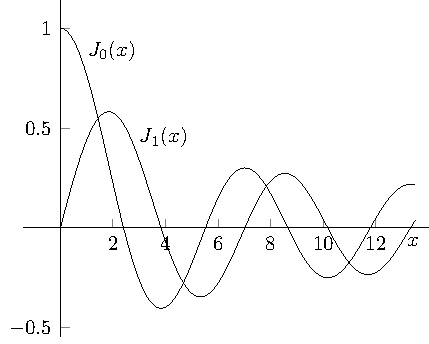
\includegraphics{figOctaveBesselFunction}
\caption{بیسل تفاعل کی پہلی قسم۔ \عددی{J_0}، \عددی{J_1}}
\label{شکل_بیسل_تفاعل}
\end{figure}
مساوات \حوالہ{مساوات_بیسل_الف} کو \عددی{x^2} سے تقسیم کرتے ہوئے  معیاری صورت \عددی{y''+\tfrac{1}{x}y'+(1-\tfrac{\nu^2}{x^2})y=0} ملتی ہے جس پر توجہ دیں۔ \عددی{x} کی زیادہ قیمت پر \عددی{\tfrac{1}{x}} اور \عددی{\tfrac{\nu^2}{x^2}} کو رد کرتے ہوئے بیسل مساوات سے \عددی{y''+y=0} حاصل ہوتا ہے جس کے حل \عددی{\cos x} اور \عددی{\sin x} ہیں۔آپ یہ بھی دیکھ سکتے ہیں کہ \عددی{\tfrac{y'}{x}} بطور تقصیری مستقل کردار ادا کرتے ہوئے بیسل تفاعل کا حیطہ گھٹانے میں مدد دے گی۔ زیادہ \عددی{x} کی صورت میں درج ذیل ثابت کیا جا سکتا ہے
\begin{align}\label{مساوات_بیسل_ذ}
J_n(x) \sim \sqrt{\frac{2}{\pi x}} \cos(x-\frac{n\pi}{2}-\frac{\pi}{4})
\end{align}
جہاں \عددی{\sim} کو \اصطلاح{متقاربی برابر}\فرہنگ{متقارب}\حاشیہب{asymptotically equal}\فرہنگ{asymptotically equal} پڑھیں اور جس کا مطلب ہے کہ کسی بھی قطعی \عددی{n} پر دونوں اطراف کی شرح، \عددی{x \to \infty} پر اکائی کے برابر ہو گی۔ 

مساوات \حوالہ{مساوات_بیسل_ذ} کم \عددی{x (>0)} کی صورت میں بھی بہترین ثابت ہوتی ہے۔اس کو استعمال کرتے ہوئے \عددی{J_0(x)} کے ابتدائی تین صفر \عددی{2.356}، \عددی{5.498} اور \عددی{8.639} حاصل ہوتے ہیں جبکہ ان کی حقیقی قیمتیں بالترتیب \عددی{2.405}، \عددی{5.520} اور \عددی{8.654} ہیں۔دونوں جوابات میں فرق \عددی{0.049}، \عددی{0.022} اور \عددی{0.015} ہے۔
\انتہا{مثال}
%=======================

\جزوحصہء{بیسل تفاعل جہاں \عددی{\nu \ge 0} کوئی بھی قیمت ہو سکتی ہے۔ گیما تفاعل}
گزشتہ حصے میں ہم نے عدد صحیح \عددی{\nu=n}کی صورت میں بیسل مساوات کا ایک حل دریافت کیا۔آئیں اب کسی بھی قیمت کے \عددی{\nu>0} کے لئے بیسل تفاعل کا عمومی حل تلاش کریں۔مساوات \حوالہ{مساوات_بیسل_عددی_سر_الف} میں ہم نے \عددی{a_0=\tfrac{1}{2^nn!}} چننا جبکہ موجودہ صورت میں ہم
\begin{align}\label{مساوات_بیسل_عددی_سر_عمومی}
a_0=\frac{1}{2^\nu \Gamma (\nu+1)}
\end{align}
چنتے ہیں جہاں \اصطلاح{گیما تفاعل}\فرہنگ{گیما تفاعل}\حاشیہب{gamma function}\فرہنگ{gamma function} \عددی{\Gamma} کی تعریف درج ذیل ہے۔
\begin{align}\label{مساوات_بیسل_گیما_الف}
\Gamma(\nu+1)=\int_{0}^{\infty}e^{-t} t^{\nu}\dif t\quad \quad (\nu >-1)
\end{align}
دھیان رہے کہ بائیں ہاتھ \عددی{\nu+1} جبکہ دائیں ہاتھ تکمل کے اندر \عددی{\nu} لکھا گیا ہے۔تکمل بالحصص سے
\begin{align*}
\Gamma(\nu+1)=\left. -e^{-t}t^{\nu}\right|_{0}^{\infty}+\nu\int_{0}^{\infty} e^{-t}t^{\nu-1}\dif t=0+\nu\Gamma(\nu)
\end{align*}
یعنی گیما تفاعل کا بنیادی تعلق
\begin{align}\label{مساوات_بیسل_گیما_ب}
\Gamma(\nu+1)=\nu\Gamma(\nu)
\end{align}
حاصل ہوتا ہے۔مساوات \حوالہ{مساوات_بیسل_گیما_الف} میں \عددی{\nu=0} پر کرنے سے 
\begin{align*}
\Gamma(1)=\int_{0}^{\infty}e^{-t}\dif t=\left.-e^{-t}\right|_{0}^{\infty}=0-(-1)=1
\end{align*}
ملتا ہے۔اس طرح مساوات \حوالہ{مساوات_بیسل_گیما_ب} سے \عددی{\Gamma(2)=1\cdot \Gamma(1)=1!}، \عددی{\Gamma(3)=3\Gamma(2)=2!} اور یوں 
\begin{align}\label{مساوات_بیسل_گیما_بطور_عدد_ضربیہ}
\Gamma(n+1)=n!\quad \quad n=0,1,2,\cdots
\end{align}
حاصل ہوتا ہے۔آپ دیکھ سکتے ہیں کہ عدد ضربی درحقیقت گیما تفاعل کی ایک مخصوص صورت ہے۔یوں عدد صحیح \عددی{\nu =n} کی صورت میں مساوات \حوالہ{مساوات_بیسل_عددی_سر_عمومی} سے مساوات \حوالہ{مساوات_بیسل_عددی_سر_الف} ہی حاصل ہوتی ہے۔

گیما تفاعل سے \عددی{0!} کی قیمت حاصل کرتے ہیں۔چونکہ \عددی{\Gamma(n+1)=n!} ہے لہٰذا 
\begin{align}\label{مساوات_بیسل_گیما_پ}
0!=\Gamma(1)=1
\end{align}
کے برابر ہے۔

مساوات \حوالہ{مساوات_بیسل_عددی_سر_عمومی} استعمال کرتے ہوئے  مساوات \حوالہ{مساوات_بیسل_چ} کو لکھتے ہیں۔
\begin{align*}
a_{2m}=\frac{(-1)^m }{2^{2m}m!(n+1)(n+2)\cdots (n+m)2^{\nu}\Gamma(\nu+1)}
\end{align*}
اب مساوات \حوالہ{مساوات_بیسل_گیما_ب} کے تحت \عددی{(\nu+1)\Gamma(\nu+1)=\Gamma(\nu+2)}، 
\عددی{(\nu+2)\Gamma(\nu+2)=\Gamma(\nu+3)} وغیرہ لکھے جا سکتے ہیں اور یوں
\begin{align*}
(\nu+1)(\nu+2)\cdots (\nu+m)\Gamma(\nu+1)=\Gamma(\nu+m+1)
\end{align*}
لکھا جا سکتا ہے۔اس طرح  
\begin{align}
a_{2m}=\frac{(-1)^m}{2^{2m+\nu}m!\Gamma(\nu+m+1)}
\end{align}
لکھا جا سکتا ہے جس کو استعمال کرتے ہوئے \عددی{r=r_1=\nu} کی صورت میں بیسل مساوات \حوالہ{مساوات_بیسل_الف} کا مخصوص حل درج ذیل حاصل ہوتا ہے۔
\begin{align}\label{مساوات_بیسل_تسلسل_عمومی}
J_{\nu}(x)=x^{\nu}\sum_{m=0}^{\infty}\frac{(-1)^m x^{2m}}{2^{2m+\nu}m!\Gamma(\nu+m+1)}
\end{align}
\عددی{J_{\nu}(x)} کو \اصطلاح{درجہ} \عددی{\nu} \اصطلاح{بیسل تفاعل کی پہلی قسم}\فرہنگ{بیسل تفاعل!پہلی قسم درجہ \عددی{\nu}}\حاشیہب{Bessel function of order $\nu$}\فرہنگ{Bessel function!first order} کہتے ہیں۔

جیسا آپ شرح عدد سر کی ترکیب سے ثابت کر سکتے ہیں، مساوات \حوالہ{مساوات_بیسل_تسلسل_عمومی} تمام \عددی{x} پر مرتکز ہے۔
%=========================
\ابتدا{مثال}
درج ذیل ثابت کریں۔
\begin{align}\label{مساوات_بیسل_گیما_نیم}
\Gamma(\tfrac{1}{2})=\sqrt{\pi}
\end{align}
حل:مساوات \حوالہ{مساوات_بیسل_گیما_الف} میں \عددی{\nu=-\tfrac{1}{2}} پر کرتے ہوئے 
\begin{align*}
\Gamma(\tfrac{1}{2})=\int_{0}^{\infty}e^{-t} t^{-\tfrac{1}{2}}\dif t
\end{align*}
ملتا ہے جس میں متغیرہ تبدیل کرتے ہوئے \عددی{t=u^2} استعمال کرتے ہیں۔
\begin{align*}
\Gamma(\tfrac{1}{2})=2\int_{0}^{\infty}e^{-u^2}\dif u
\end{align*}
اب ہم ایک ترکیب استعمال کرتے ہیں (جس کو ذہن نشین کرنا سود مند ثابت ہو گا)۔ درج بالا میں \عددی{u} کی جگہ \عددی{w} بھی لکھا جا سکتا ہے۔ایسا کرتے ہوئے 
\begin{align*}
\Gamma(\tfrac{1}{2})=2\int_{0}^{\infty}e^{-w^2}\dif w
\end{align*}

ملتا ہے۔درج بالا دو مساوات کو آپس میں ضرب دیتے ہیں۔
\begin{align*}
\Gamma(\tfrac{1}{2})^2=4\int_{0}^{\infty}e^{-u^2}\dif u \int_{0}^{\infty}e^{-w^2}\dif w=4\int_{0}^{\infty}\int_{0}^{\infty} e^{-(u^2+w^2)}\dif u\dif w
\end{align*}
یہ تکمل کارتیسی محور کے ربع اول پر حاصل کیا گیا ہے۔اس تکمل کو نلکی محور \عددی{r} اور \عددی{\theta} استعمال کرتے ہوئے حاصل کیا جا سکتا ہے۔یوں \عددی{u=r\cos \theta} اور \عددی{w=r\sin \theta} لیتے ہیں۔ چھوٹا رقبہ \عددی{\dif u\dif w=r\dif r\dif \theta} لکھا جائے گا۔ربع اول میں \عددی{r} کے حدود \عددی{0} تا \عددی{\infty} اور \عددی{\theta} کے حدود \عددی{0} تا  \عددی{\tfrac{\pi}{2}} ہیں۔
\begin{align*}
\Gamma(\tfrac{1}{2})^2=4\int_{0}^{\tfrac{\pi}{2}}\int_{0}^{\infty} e^{-r^2} r\dif r\dif \theta=4\int_{0}^{\frac{\pi}{2}}\left. -\frac{1}{2}e^{-r^2}\right|_{0}^{\infty} \dif \theta=4\left(\frac{1}{2}\right)\frac{\pi}{2}=\pi
\end{align*}
ملتا ہے۔دونوں اطراف کا جذر لینے سے \عددی{\Gamma(\tfrac{1}{2})=\sqrt{\pi}} ملتا ہے۔
\انتہا{مثال}
%================================
\جزوحصہء{خواص بیسل تفاعل}
بیسل تفاعل انتہائی زیادہ تعلقات پر پورا اترتے ہیں۔آئیں درج ذیل تعلقات کو بیسل تسلسل سے اخذ کریں۔
\begin{align}
[x^{\nu}J_{\nu}(x)]'&=x^{\nu}J_{\nu-1}(x) \label{مساوات_بیسل_تعلق_الف}\\
[x^{-\nu}J_{\nu}(x)]'&=-x^{-\nu}J_{\nu+1}(x) \label{مساوات_بیسل_تعلق_ب}\\
J_{\nu-1}(x)+J_{\nu+1}(x)&=\frac{2\nu}{x}J_{\nu}(x) \label{مساوات_بیسل_تعلق_پ}\\
J_{\nu-1}(x)-J_{\nu+1}(x)&=2J'_{\nu}(x) \label{مساوات_بیسل_تعلق_ت}
\end{align}
مساوات \حوالہ{مساوات_بیسل_تعلق_الف} ثابت کرتے ہیں۔مساوات \حوالہ{مساوات_بیسل_تسلسل_عمومی} کو \عددی{x^{\nu}} سے ضرب دیتے ہوئے
\begin{align*}
x^{\nu}J_{\nu}(x)=\sum_{m=0}^{\infty}\frac{(-1)^m x^{2m+2\nu}}{2^{2m+\nu}m!\Gamma(\nu+m+1)}
\end{align*}
تفرق لے کر مساوات \حوالہ{مساوات_بیسل_گیما_ب} سے \عددی{\Gamma(\nu+m+1)=(\nu+m)\Gamma(\nu+m)} لکھ کر ترتیب دیتے ہیں۔
\begin{multline*}
[x^{\nu}J_{\nu}(x)]'=\sum_{m=0}^{\infty}\frac{(2m+2\nu)(-1)^m x^{2m+2\nu-1}}{2^{2m+\nu}m!\Gamma(\nu+m+1)}=\sum_{m=0}^{\infty}\frac{2(m+\nu)(-1)^m x^{2m+2\nu-1}}{2^{2m+\nu}m!(\nu+m)\Gamma(\nu+m)}\\
=\sum_{m=0}^{\infty}\frac{(-1)^m x^{2m+2\nu-1}}{2^{2m+\nu-1}m!\Gamma(\nu+m)}=x^{\nu}x^{\nu-1}\sum_{m=0}^{\infty}\frac{(-1)^m x^{2m}}{2^{2m+\nu-1}m!\Gamma(\nu+m)}=x^{\nu}J_{\nu-1}(x)
\end{multline*}
آخری قدم مساوات \حوالہ{مساوات_بیسل_تسلسل_عمومی} میں \عددی{\nu} کی جگہ \عددی{\nu-1} پر کر کے موازنہ کرتے ہوئے لکھا گیا ہے۔

آئیں اب مساوات \حوالہ{مساوات_بیسل_تعلق_ب} ثابت کریں۔مساوات \حوالہ{مساوات_بیسل_تسلسل_عمومی} کو \عددی{x^{-\nu}} سے ضرب دینے سے \عددی{x^{\nu}} کٹ جاتا ہے۔
\begin{align*}
x^{-\nu}J_{\nu}(x)=\sum_{m=0}^{\infty}\frac{(-1)^m x^{2m}}{2^{2m+\nu}m!\Gamma(\nu+m+1)}
\end{align*}
تفرق لے کر \عددی{m!=m(m-1)!} لکھ کر ترتیب دیتے ہیں۔
\begin{align*}
[x^{-\nu}J_{\nu}(x)]'=\sum_{m=1}^{\infty}\frac{2m(-1)^m x^{2m-1}}{2^{2m+\nu}m!\Gamma(\nu+m+1)}=\sum_{m=1}^{\infty}\frac{2m(-1)^m x^{2m-1}}{2^{2m+\nu}m(m-1)!\Gamma(\nu+m+1)}\\
=\sum_{m=1}^{\infty}\frac{(-1)^m x^{2m-1}}{2^{2m+\nu-1}(m-1)!\Gamma(\nu+m+1)}
\end{align*}
دھیان رہے کہ تفرق کے بعد تسلسل کا پہلا رکن \عددی{m=1} سے ظاہر کیا جائے گا۔(آپ \عددی{x^{-\nu}J_{\nu}} کے تسلسل کو پھیلا کر لکھ کر تفرق لیتے ہوئے دیکھ سکتے ہیں کہ پہلا رکن \عددی{m=1} ہے)۔ درج بالا تسلسل میں \عددی{s=m-1} یعنی \عددی{m=s+1} پر کرتے ہیں۔
\begin{align*}
[x^{-\nu}J_{\nu}(x)]'=\sum_{s=0}^{\infty}\frac{(-1)^{s+1} x^{2s+1}}{2^{2s+\nu+1}s!\Gamma(\nu+s+2)}=-x^{-\nu}J_{\nu+1}(x)
\end{align*}
آخری قدم مساوات \حوالہ{مساوات_بیسل_تسلسل_عمومی} میں \عددی{\nu} کی جگہ \عددی{\nu+1} پر کر کے موازنہ کرتے ہوئے لکھا گیا ہے۔

اب مساوات \حوالہ{مساوات_بیسل_تعلق_پ} اور مساوات \حوالہ{مساوات_بیسل_تعلق_پ} ثابت کرتے ہیں۔مساوات \حوالہ{مساوات_بیسل_تعلق_الف} اور مساوات \حوالہ{مساوات_بیسل_تعلق_ب} کو درج ذیل لکھا جا سکتا ہے۔
\begin{align*}
\nu x^{\nu-1} J_{\nu}+x^{\nu}J'_{\nu}&=x^{\nu} J_{\nu-1}\\
-\nu x^{-\nu-1} J_{\nu}+x^{-\nu}J'_{\nu}&=-x^{-\nu} J_{\nu+1}
\end{align*}
پہلی مساوات کو \عددی{x^{\nu}} اور دوسری مساوات کو \عددی{x^{-\nu}} سے تقسیم کرتے ہیں۔
\begin{align*}
\nu x^{-1} J_{\nu}+J'_{\nu}&= J_{\nu-1}\\
-\nu x^{-1} J_{\nu}+J'_{\nu}&=-J_{\nu+1}
\end{align*}
ان کو جمع اور تفریق کرتے ہوئے درج ذیل (درکار) مساوات ملتے ہیں۔
\begin{align*}
2J'_{\nu}&=J_{\nu-1}-J_{\nu+1}\\
\frac{2\nu}{x}J_{\nu}&=J_{\nu-1}+J_{\nu+1}
\end{align*}
%================================
\ابتدا{مثال}\quad مساوات \حوالہ{مساوات_بیسل_تعلق_الف} تا مساوات \حوالہ{مساوات_بیسل_تعلق_ت} کا استعمال\\
درج ذیل کو \عددی{J_0} اور \عددی{J_1} کی صورت میں حاصل کریں۔
\begin{align*}
\int_{1}^{2} x^{-3}J_4(x)\dif x
\end{align*}

حل:مساوات \حوالہ{مساوات_بیسل_تعلق_ب} میں \عددی{\nu=3} لیتے ہوئے  درج ذیل ملتا ہے۔
\begin{align*}
I=\int_{1}^{2} x^{-3}J_4(x)\dif x=\left. -x^{-3}J_3(x)\right|_{1}^{2}
\end{align*}
مساوات \حوالہ{مساوات_بیسل_تعلق_پ} میں \عددی{\nu=2} پر کرتے ہوئے \عددی{J_3=\tfrac{4}{x}J_2-J_1} اور \عددی{\nu=1} پر کرتے ہوئے \عددی{J_2=\tfrac{2}{x}J_1-J_0} لکھا جا سکتا ہے لہٰذا \عددی{J_3=\tfrac{4}{x}(\tfrac{2}{x}J_1-J_0)-J_1} لکھا جا سکتا ہے۔یوں تکمل کی قیمت
\begin{align*}
I=\left.  -x^{-3}[4x^{-1}(2x^{-1}J_1-J_0)-J_0] \right|_{1}^{2}=-\frac{1}{8}J_1(2)+\frac{1}{4}J_0(2)+7J_1(1)-4J_0(1)
\end{align*}
ہو گی۔
\انتہا{مثال}
%===========================
\ابتدا{مثال}
درج ذیل (شکل \حوالہ{شکل_بیسل_کسری_بیسل}) ثابت کریں۔
\begin{gather}
\begin{aligned} \label{مساوات_بیسل_تعلق_کوسائن}
J_{\frac{1}{2}}(x)&=\sqrt{\frac{2}{\pi x}}\sin x\\
J_{-\frac{1}{2}}(x)&=\sqrt{\frac{2}{\pi x}}\cos x
\end{aligned}
\end{gather}
حل:بیسل تسلسل \حوالہ{مساوات_بیسل_تسلسل_عمومی} میں \عددی{\nu=\tfrac{1}{2}} پر کرتے ہوئے ہیں۔
\begin{align*}
J_{\frac{1}{2}}(x)=\sqrt{x}\sum_{m=0}^{\infty}\frac{(-1)^m x^{2m}}{2^{2m+\frac{1}{2}}m!\Gamma(\frac{1}{2}+m+1)}=\sqrt{\frac{2}{x}}\sum_{m=0}^{\infty}\frac{(-1)^m x^{2m+1}}{2^{2m+1}m!\Gamma(m+\frac{3}{2})}
\end{align*}
نسب نما میں درج ذیل لکھا جا سکتا ہے جہاں آخری قدم پر مساوات \حوالہ{مساوات_بیسل_گیما_نیم} استعمال کیا گیا ہے۔
\begin{align*}
2^mm!&=2m(2m-2)(2m-4)\cdots 4\cdot 2\\
2^{m+1}\Gamma(m+\tfrac{3}{2})&=2^{m+1}(m+\tfrac{1}{2})(m-\tfrac{1}{2})\cdots \tfrac{3}{2}\cdot \Gamma(\tfrac{1}{2})\\
&=(2m+1)(2m-1)\cdots 3\cdot 2\cdot 1\cdot \sqrt{\pi}
\end{align*}
ان نتائج کو استعمال کرتے ہوئے نسب نما میں
\begin{align*}
2^{2m+1}m!\Gamma(m+\tfrac{3}{2})=(2m+1)2m(2m-1)(2m-2)\cdots 3\cdot 2 \cdot 1\cdot \sqrt{\pi}=(2m+1)!\sqrt{\pi}
\end{align*}
لکھا جا سکتا ہے لہٰذا درج ذیل ثابت ہوتا ہے۔
\begin{align*}
J_{\frac{1}{2}}(x)=\sqrt{\frac{2}{\pi x}}\sum_{m=0}^{\infty}\frac{(-1)^m x^{2m+1}}{(2m+1)!}=\sqrt{\frac{2}{\pi x}}\sin x
\end{align*}
%
\begin{figure}
\centering
\begin{tikzpicture}
\begin{axis}[axis lines*=middle,xlabel=x,xlabel style={at={(current axis.right of origin)},anchor=north east},ytick={0,1},yticklabels={$0$,$1$},xtick={6.28,12.57,18.85},xticklabels={$2\pi$,$4\pi$,$6\pi$},ymax=1]
\addplot[domain=0:20,samples=100]{sqrt(2/(pi*x))*sin(180/pi*x)};
\addplot[domain=0.2:20,samples=100]{sqrt(2/(pi*x))*cos(180/pi*x)};
\end{axis}
\end{tikzpicture}
\caption{بیسل تفاعل \عددی{J_{\tfrac{1}{2}}(x)} اور \عددی{J_{-\tfrac{1}{2}}(x)}}
\label{شکل_بیسل_کسری_بیسل}
\end{figure}

مساوت \حوالہ{مساوات_بیسل_تعلق_الف} استعمال کرتے ہوئے
\begin{align*}
[\sqrt{x}J_{\tfrac{1}{2}}(x)]'=\sqrt{\frac{2}{\pi}}\cos x=\sqrt{x}J_{-\tfrac{1}{2}}(x)
\end{align*} 
لکھا جا سکتا ہے جس میں دائیں ہاتھ کے مساوات کو لیتے ہوئے \عددی{\sqrt{x}} سے تقسیم کرتے ہوئے مساوات \حوالہ{مساوات_بیسل_تعلق_کوسائن} کی دوسری مساوات ملتی ہے۔
\انتہا{مثال}
%=============================

\جزوحصہء{عمومی حل۔ خطی طور تابعیت}
بیسل مساوات \حوالہ{مساوات_بیسل_الف} کے عمومی حل کے لئے \عددی{J_v(x)} کے علاوہ خطی طور غیر تابع دوسرا حل بھی درکار ہے۔غیر عدد صحیح \عددی{\nu} کی صورت میں دوسرا حل  \عددی{r_2=-\nu} (اشاری مساوات \حوالہ{مساوات_بیسل_ت}) استعمال کرتے ہوئے حاصل ہو گا۔یوں دوسرا خطی طور غیر تابع حل مساوات \حوالہ{مساوات_بیسل_تسلسل_عمومی} میں \عددی{\nu} کی جگہ \عددی{-\nu} پر کرنے سے حاصل ہو گا۔
\begin{align}\label{مساوات_بیسل_تسلسل_عمومی_دوسرا}
J_{-\nu}(x)=x^{-\nu}\sum_{m=0}^{\infty}\frac{(-1)^m x^{2m}}{2^{2m-\nu}m!\Gamma(m-\nu+1)}
\end{align}
\عددی{\nu} غیر عدد صحیح ہونے کی صورت میں \عددی{J_{\nu}} اور \عددی{J_{-\nu}} خطی طور غیر تابع ہیں۔یوں غیر عدد صحیح \عددی{\nu} کی صورت میں \عددی{x \ne 0} پر  مساوات بیسل کا عمومی حل 
\begin{align}
y(x)=c_1J_{\nu}(x)+c_2J_{-\nu}(x)
\end{align}
ہو گا۔ 

\عددی{\nu} عدد صحیح ہونے کی صورت میں \عددی{J_n(x)} اور \عددی{J_{-n}(x)} کا تعلق
\begin{align}\label{مساوات_بیسل_عدد_صحیح_بیسل_تعلق}
J_{-n}(x)=(-1)^nJ_n(x) \quad \quad (n=1,2,\cdots)
\end{align}
ہے لہٰذا یہ خطی طور تابع ہیں اور ان سے عمومی حل نہیں لکھا جا سکتا ہے۔آئیں مساوات \حوالہ{مساوات_بیسل_عدد_صحیح_بیسل_تعلق} کو ثابت کریں۔

%==============================
\ابتدا{ثبوت}
مساوات \حوالہ{مساوات_بیسل_تسلسل_عمومی_دوسرا} میں \عددی{\nu} کی قیمت کو عدد صحیح کے قریب تر لانے سے گیما تفاعل کی قیمت (صفحہ \حوالہصفحہ{شکل_ضمیمہ_گیما_تفاعل} پر شکل \حوالہ{شکل_ضمیمہ_گیما_تفاعل}) لامتناہی کی طرف بڑھتی ہے۔یوں \عددی{\nu=n} کی صورت میں مساوات \حوالہ{مساوات_بیسل_تسلسل_عمومی_دوسرا} کے ابتدائی \عددی{n} ارکان کے عددی سر، گیما تفاعل کی قیمت لامتناہی ہونے کی بنا، صفر ہوں گے اور یوں تسلسل \عددی{m=n} سے شروع ہو گا۔مساوات \حوالہ{مساوات_بیسل_گیما_بطور_عدد_ضربیہ} کے تحت \عددی{\Gamma(m-n+1)=(m-n)!} ہے لہٰذا درج ذیل لکھا جائے گا
\begin{align*}
J_{-n}(x)=\sum_{m=n}^{\infty}\frac{(-1)^mx^{2m-n}}{2^{2m-n}m!(m-n)!}=\sum_{s=0}^{\infty}\frac{(-1)^{n+s}x^{2s+n}}{2^{2s+n} (n+s)!s!}\quad \quad (m=n+s)
\end{align*}
جو \عددی{(-1)^nJ_n(x)} ہے۔
\انتہا{ثبوت}
%==========================

اگلے حصے میں \عددی{\nu=n} کی صورت میں مساوات بیسل کا عمومی حل، بیسل تفاعل کی دوسری قسم \عددی{Y_{\nu}} کی مدد سے، حاصل کیا جائے گا۔
%==================

\حصہء{سوالات}

 %==================
\ابتدا{سوال}
ثابت کریں کہ \عددی{J_n(x)} تمام \عددی{x} کے لئے مرتکز ہے۔

جواب: \عددی{\abs{\tfrac{a_{m+1}}{a_m}}=\tfrac{2^{2m+n}m!(n+m)!}{2^{2m+2+n} (m+1)!(n+m+1)!}=\tfrac{1}{2^2(m+1)(n+m+1)}} ہے لہٰذا 
\عددی{\abs{\tfrac{a_{m+1}}{a_m}}_{m\to \infty}=0} اور یوں \عددی{R\to \infty} ہو گا۔
\انتہا{سوال}
%====================
سوال \حوالہ{سوال_بیسل_صورت_الف} تا سوال \حوالہ{سوال_بیسل_صورت_ب} کے عمومی حل، جہاں ممکن ہو،  \عددی{J_{\nu}} اور \عددی{J_{-\nu}} استعمال کرتے ہوئے لکھیں۔جہاں اضافی معلومات دی گئی ہوں، وہاں اس کو استعمال کرتے ہوئے بیسل مساوات کی صورت حاصل کریں۔

%============
\ابتدا{سوال}\شناخت{سوال_بیسل_صورت_الف}\quad
$x^2y''+xy'(x^2-\frac{4}{9})y=0$\\
جواب:چونکہ \عددی{\nu=\tfrac{2}{3}} ہے جو غیر عدد صحیح ہے لہٰذا عمومی حل \عددی{y=c_1J_{\tfrac{2}{3}}+c_2J_{-\tfrac{2}{3}}} ہے۔
\انتہا{سوال}
%=================
\ابتدا{سوال}\quad
$xy''+y'+\frac{1}{4}y\quad \quad (z=\sqrt{x})$\\
جواب:\عددی{y=c_1J_0(\sqrt{x})}
\انتہا{سوال}
%=================
\ابتدا{سوال}\quad
$xy''+y'+\frac{x}{4}y=0\quad \quad (z=\frac{x}{2})$\\
جواب:\عددی{y=c_1J_0(\tfrac{x}{2})}
\انتہا{سوال}
%===================
\ابتدا{سوال}\quad
$x^2y''+xy'(\frac{x^2}{9}-\frac{1}{9})y=0\quad \quad (z=\frac{x}{3})$\\
جواب:\عددی{y=c_1J_{\tfrac{1}{3}}(\tfrac{x}{3})+c_2J_{-\tfrac{1}{3}}(\tfrac{x}{3})}
\انتہا{سوال}
%====================
\ابتدا{سوال}\quad
$y''+(e^{2x}-16)y=0,\quad \quad (z=e^x)$\\
جواب:\عددی{y=c_1J_4(e^x)}
\انتہا{سوال}
%=================
\ابتدا{سوال}\quad
$x^2y''+xy'(\lambda^2 x^2-\nu^2)y=0,\quad \quad (z=\lambda x)$\\
جواب:\عددی{y=c_1 J_{\nu}(\lambda x)+c_2J_{-\nu}(\lambda x)} جہاں \عددی{\nu \ne 0, \mp1, \mp2, \cdots}
\انتہا{سوال}
%=================
\ابتدا{سوال}\quad
$x^2y''+xy'+(9x^2-1)y=0,\quad \quad (z=3x)$\\
جواب:\عددی{y=c_1J_1(3x)}
\انتہا{سوال}
%======================
\ابتدا{سوال}\quad
$(x-\frac{1}{2})^2y''+(x-\frac{1}{2})y'+4x(x-1)y=0\quad \quad(z=2x-1)$\\
جواب:\عددی{y=c_1J_1(2x-1)}
\انتہا{سوال}
%==================
\ابتدا{سوال}\quad
$xy''+(2\nu+1)y'+xy=0,\quad \quad y=x^{-\nu}u$\\
جواب:\عددی{y=x^{-\nu}(c_1J_{\nu}(x)+c_2J_{-\nu}(x))} جہاں \عددی{\nu \ne 0,\mp1,\mp2,\cdots}
\انتہا{سوال}
%====================
\ابتدا{سوال}\شناخت{سوال_بیسل_صورت_ب}\quad
$x^2y''+\frac{1}{4}(x+\frac{3}{4})y=0,\quad \quad y=u\sqrt{x}, \quad z=\sqrt{x}$\\
جواب:\عددی{y=c_1\sqrt{x}J_{\tfrac{1}{2}}(\sqrt{x})+c_2\sqrt{x}J_{-\tfrac{1}{2}}(\sqrt{x})}
\انتہا{سوال}
%====================
\ابتدا{سوال}
مساوات \حوالہ{مساوات_بیسل_تعلق_پ} اور مساوات \حوالہ{مساوات_بیسل_تعلق_کوسائن} سے درج ذیل ثابت کریں۔
\begin{align}
J_{\tfrac{3}{2}}(x)=\sqrt{\frac{2}{\pi x}} \left(\frac{\sin x}{x}-\cos x\right), \quad  J_{-\tfrac{3}{2}}(x)=-\sqrt{\frac{2}{\pi x}}\left(\frac{\cos x}{x}+\sin x \right)
\end{align}
\انتہا{سوال}
%======================
\ابتدا{سوال}
کیا آپ مساوات \حوالہ{مساوات_بیسل_تعلق_پ} اور مساوات \حوالہ{مساوات_بیسل_تعلق_کوسائن} سے  اخذ کر سکتے ہیں کہ
 \عددی{\nu=\mp \tfrac{1}{2},\mp\tfrac{3}{2},\mp\tfrac{5}{2},\cdots} کی صورت میں \عددی{J_{\nu}(x)} بنیادی تفاعل ہیں۔

جواب:جی ہاں۔
\انتہا{سوال}
%=====================

%================
\ابتدا{سوال}\quad باہم پیچاں صفر\\
مساوات \حوالہ{مساوات_بیسل_تعلق_الف}، مساوات \حوالہ{مساوات_بیسل_تعلق_ب} اور \اصطلاح{مسئلہ رول}\فرہنگ{مسئلہ!رول}\فرہنگ{رول مسئلہ}\حاشیہب{Rolle's theorem}\فرہنگ{theorem!Rolle's} استعمال کرتے ہوئے ثابت کریں کہ \عددی{J_n(x)} کے کسی بھی دو متواتر صفروں کے مابین \عددی{J_{n+1}(x)} کا ایک صفر پایا جاتا ہے۔ 

جواب:مسئلہ رول کہتا ہے کہ کسی بھی حقیقی قابل تفرق تفاعل کے دو متواتر برابر قیمت نقطوں کے مابین کم از کم ایک ایسا نقطہ (نقطہ فاصل) پایا جاتا ہے جس پر تفاعل کا تفرق صفر کے برابر ہو گا۔ اگر \عددی{J_n(x)} کے دو متواتر صفر \عددی{x_1} اور \عددی{x_2} پر پائے جاتے ہوں تب ہم \عددی{x_1^{-n}J_n(x_1)=x_2^{-n}J_n(x_2)=0} لکھ سکتے ہیں۔یوں مسئلہ رول کے تحت \عددی{x_1} اور \عددی{x_2} کے مابین کسی نقطے پر تفاعل \عددی{x^{-n}J_n(x)} کا تفرق صفر \عددی{[x^{-n}J_n(x)]'=0} ہو گا جو مساوات \حوالہ{مساوات_بیسل_تعلق_ب} کے استعمال سے ایسے نقطے پر \عددی{x^{-n}J_{n+1}(x)=0} یعنی \عددی{J_{n+1}(x)=0} دیتا ہے۔اسی طرح اگر \عددی{J_{n+1}(x)} کے دو متواتر صفر \عددی{x_3} اور \عددی{x_4} پر پائے جاتے ہوں تب \عددی{J_{n+1}(x_3)=J_{n+1}(x_4)=0} اور \عددی{x_3^{n+1}J_{n+1}(x_3)=x_4^{n+1}J_{n+1}(x_4)=0} لکھا جا سکتا ہے۔یوں مسئلہ رول کے تحت \عددی{x_3} اور \عددی{x_4} کے مابین کسی نقطے پر \عددی{[x^{n+1}J_{n+1}(x)]'=0} ہو گا جس سے مساوات \حوالہ{مساوات_بیسل_تعلق_الف} کے تحت ایسے نقطے پر \عددی{x^{n+1}J_n(x)=0} یعنی \عددی{J_n(x)=0} حاصل ہوتا ہے۔ یوں  ثابت ہوا کہ \عددی{J_{n+1}} کے دو متواتر صفر \عددی{x_3} اور \عددی{x_4} کے مابین \عددی{J_n(x)} کا صفر پایا جاتا ہے جبکہ \عددی{J_n(x)} کے دو متواتر صفر \عددی{x_1} اور \عددی{x_2} کے مابین \عددی{J_{n+1}(x)} کا صفر پایا جاتا ہے۔
\انتہا{سوال}
%=================
\ابتدا{سوال}\quad تفرقی مساوات سے ایک درجی تفرق کا اخراج\\
 درج ذیل تفرقی مساوات میں \عددی{y(x)=u(x)v(x)} پر کرتے ہوئے ایسا \عددی{v(x)} دریافت کریں کہ حاصل تفرقی مساوات میں پہلے درجے کا تفرق نہ پایا جاتا ہو۔حاصل تفرقی مساوات بھی حاصل کریں۔
\begin{align*}
y''+p(x)y'+q(x)y=0
\end{align*}
جوابات:\عددی{v=e^{-\tfrac{1}{2}\int p(x)\dif x}} اور مساوات \عددی{u''+[q-\tfrac{1}{4}p^2-\tfrac{1}{2}p']u=0} میں \عددی{u'} نہیں پایا جاتا ہے۔

\انتہا{سوال}
%=====================
\ابتدا{سوال}
گزشتہ سوال میں تفرقی مساوات سے ایک درجی تفرق کا اخراج کیا گیا۔ثابت کریں کہ مساوات بیسل \حوالہ{مساوات_بیسل_الف} سے ایک درجی تفرق کا اخراج \عددی{y=\tfrac{u}{\sqrt{x}}} پر کرتے ہوئے ہو گا جس سے درج ذیل تفرقی مساوات حاصل ہو گی۔
\begin{align}\label{مساوات_بیسل_سادہ_صورت}
x^2u''+(x^2+\tfrac{1}{4}-\nu^2)u=0
\end{align}
\انتہا{سوال}
%====================
\ابتدا{سوال}
مساوات \حوالہ{مساوات_بیسل_سادہ_صورت} کا عمومی حل \عددی{\nu=\tfrac{1}{2}} کے لئے حاصل کریں۔

جواب: \عددی{u=A\cos x+B\sin x} ہے لہٰذا \عددی{y=\tfrac{u}{\sqrt{x}}=\tfrac{1}{\sqrt{x}}(A\cos x+B\sin x)} ہو گا۔
\انتہا{سوال}
%===================
سوال \حوالہ{سوال_بیسل_تفرق_تکمل_الف} تا سوال \حوالہ{سوال_بیسل_تفرق_تکمل_ب}  مساوات \حوالہ{مساوات_بیسل_تعلق_الف} اور مساوات \حوالہ{مساوات_بیسل_تعلق_ب} کی مدد سے حل ہوں گے۔

%===============
\ابتدا{سوال}\شناخت{سوال_بیسل_تفرق_تکمل_الف}\quad ثابت کریں 
$J'_0(x)=-J_1(x),\quad J'_1(x)=J_0(x)-\frac{J_1(x)}{x},\quad J'_2(x)=\frac{1}{2}[J_1(x)-J_3(x)]$\\
\انتہا{سوال}
%=================
\ابتدا{سوال}
بیسل مساوات \حوالہ{مساوات_بیسل_الف} کو مساوات \حوالہ{مساوات_بیسل_تعلق_الف} اور مساوات \حوالہ{مساوات_بیسل_تعلق_ب} سے حاصل کریں۔
\انتہا{سوال}
%=====================
\ابتدا{سوال}
درج ذیل ثابت کریں
\begin{align*} 
\int x^{\nu} J_{\nu-1}(x)\dif x&=x^{\nu}J_{\nu}(x)+c\\
\int x^{-\nu}J_{\nu+1}\dif x&=-x^{-\nu}J_{\nu}(x)+c\\
\int J_{\nu+1}(x)\dif x&=\int J_{\nu-1}(x)\dif x-2J_{\nu}(x)
\end{align*}
\انتہا{سوال}
%======================
\ابتدا{سوال}\quad
$\int J_3(x)\dif x$\\
جواب:مساوات \حوالہ{مساوات_بیسل_تعلق_ت} میں \عددی{\nu=2} پر کر کے تکمل \عددی{\int J_3\dif x=\int  J_1\dif x-2J_2} ہو گا اور مساوات \حوالہ{مساوات_بیسل_تعلق_ب} میں \عددی{\nu=0} پر کرتے ہوئے تکمل \عددی{\int J_1\dif x=-J_0} دیتا ہے لہٰذا \عددی{\int J_3\dif x=-J_0-2J_2+c} 
\انتہا{سوال}
%=====================
\ابتدا{سوال} تکمل بالحصص استعمال کرتے  ہوئے حل کریں۔\quad 
$\int x^3J_0(x)\dif x$\\
جواب:
$\int x^3J_0\dif x=\int x^2(xJ_0)\dif x=x^2(xJ_1)-2\int x^2J_1\dif x=x^3J_1-2x^2J_2+c$
\انتہا{سوال}
%=======================
\ابتدا{سوال} \شناخت{سوال_بیسل_تفرق_تکمل_ب} تکمل بالحصص سے حل کریں۔\quad 
$\int x^2J_0\dif x$\\
جواب:\عددی{\int x^2J_0\dif x=x^2J_1+xJ_0-\int J_0\dif x}، جہاں \عددی{\int J_0\dif x} کسی بنیادی تفاعل کی صورت میں نہیں لکھا جا سکتا ہے بلکہ اس کی قیمت  جدول کی مدد سے لکھی جاتی ہے۔

\انتہا{سوال}
%===================

\حصہ{بیسل تفاعل کی دوسری قسم۔ عمومی حل}
بیسل مساوات \حوالہ{مساوات_بیسل_الف} کا کسی بھی \عددی{\nu} کے لئے عمومی حل حاصل کرنے کی خاطر \اصطلاح{بیسل تفاعل کی دوسری قسم}\فرہنگ{بیسل تفاعل!دوسری قسم}\حاشیہب{Bessel function of the second kind}\فرہنگ{Bessel!second kind function} \عددی{Y_{\nu}(x)} حاصل کرتے ہیں۔شروع \عددی{\nu=n=0} سے کرتے ہیں۔  

\عددی{n=0} کی صورت میں مساوات بیسل کو \عددی{x} سے تقسیم کرتے ہوئے
\begin{align}\label{مساوات_بیسل_دوہرا_صفر_الف}
xy''+y'+xy=0
\end{align}
لکھا جا سکتا ہے اور اشاری مساوات \حوالہ{مساوات_طاقتی_اشاری_مساوات} سے دوہرا جذر \عددی{r=0} ملتا ہے  جو صفحہ \حوالہصفحہ{مسئلہ_طاقتی_فروبنیوس_اساس} پر مسئلہ فروبنیوس میں بتلائی گئی دوسری صورت کو ظاہر کرتی ہے۔یوں مساوات \حوالہ{مساوات_بیسل_دوہرا_صفر_الف} کا ایک حل \عددی{J_0(x)} ہو گا جبکہ اس کا دوسرا حل مساوات \حوالہ{مساوات_طاقتی_فروبنیوس_حل_ت} میں \عددی{r=0} پر کرتے ہوئے  
\begin{align}\label{مساوات_بیسل_دوہرا_صفر_ب}
y_2(x)=J_0(x)\ln x+\sum_{m=1}^{\infty}A_m x^m 
\end{align}
لکھا جائے گا۔مساوات \حوالہ{مساوات_بیسل_دوہرا_صفر_ب} اور اس کے تفرقات
\begin{align*}
y_2'&=J_0' \ln x+\frac{J_0}{x}+\sum_{m=1}^{\infty}mA_mx^{m-1}\\
y_2''&=J_0''\ln x+\frac{2J_0'}{x}-\frac{J_0}{x}+\sum_{m=1}^{\infty} m(m-1)A_m x^{m-2}
\end{align*}
کو مساوات \حوالہ{مساوات_بیسل_دوہرا_صفر_الف} میں پر کرتے ہیں (اگرچہ آخری مجموعے کا پہلا رکن \عددی{m=2} لکھنا چاہیے، البتہ \عددی{m=1} پر دیا گیا مجموعہ صفر دیتا ہے لہٰذا مجموعے کا پہلا رکن \عددی{m=1} لکھنا ممکن ہے)۔اب چونکہ \عددی{J_0} تفرقی مساوات کا حل ہے لہٰذا  تین لوگارتھمی ارکان کا مجموعہ \عددی{(xJ_0''+J_0'+xJ_0)\ln x} صفر کے برابر ہو گا اور یوں بقایا درج ذیل ہو گا۔
\begin{align*}
2J_0'+\sum_{m=1}^{\infty}m(m-1)A_mx^{m-1}+\sum_{m=1}^{\infty}mA_mx^{m-1}+\sum_{m=1}^{\infty}A_mx^{m+1}=0
\end{align*}
اس میں پہلے اور دوسرے  مجموعوں کو جمع کرتے ہوئے \عددی{\sum m^2A_mx^{m-1}} لکھا کر جبکہ \عددی{J_0'} کی طاقتی تسلسل کو مساوات \حوالہ{مساوات_بیسل_د} کا جزو در جزو تفرق لیتے اور \عددی{\tfrac{m!}{m}=(m-1)!} استعمال کرتے ہوئے
\begin{align*}
J'_0(x)=\sum_{m=1}^{\infty}\frac{(-1)^m2mx^{2m-1}}{2^{2m}(m!)^2}=\sum_{m=1}^{\infty}\frac{(-1)^mx^{2m-1}}{2^{2m-1}m!(m-1)!}
\end{align*} 
لکھ کر درج ذیل حاصل ہوتا ہے۔
\begin{align}\label{مساوات_بیسل_دوہرا_صفر_پ}
\sum_{m=1}^{\infty}\frac{(-1)^mx^{2m-1}}{2^{2m-2}m!(m-1)!}+\sum_{m=1}^{\infty} m^2A_mx^{m-1}+\sum_{m=1}^{\infty}A_mx^{m+1}=0
\end{align}
اس مساوات میں \عددی{x^0} کمتر طاقت، جو صرف دوسرے مجموعے میں پایا جاتا ہے، کے عددی سر کو صفر کے برابر پر کرتے ہوئے \عددی{A_1=0} ملتا ہے۔اب \عددی{x^{2s}} کے عددی سروں، جو پہلے تسلسل میں نہیں پایا جاتا، کے مجموعے کو صفر کے برابر لکھتے ہیں۔
\begin{align*}
(2s+1)^2A_{2s+1}+A_{2s-1}=0,\quad \quad (s=1,2,\cdots)
\end{align*}
اب چونکہ \عددی{A_1=0} ہے لہٰذا \عددی{A_3=0}، \عددی{A_5=0}، \نقطے ہوں گے۔ 

\عددی{x^{2s+1}} کے عددی سروں کے مجموعے کو صفر کے برابر پر کرتے ہوئے \عددی{s=0} کے لئے
\begin{align*}
-1+4A_2=0, \quad \implies \quad A_2=\frac{1}{4}
\end{align*}
جبکہ بقایا \عددی{s} پر
\begin{align*}
\frac{(-1)^{s+1}}{2^{2s}(s+1)!s!}+(2s+2)^2A_{2s+2}+A_{2s}=0,\quad (s=1,2,\cdots)
\end{align*}
لکھا جائے گا۔اس سے \عددی{s=1} کے لئے
\begin{align*}
\frac{1}{8}+16A_4+A_2=0\quad \implies \quad A_4=-\frac{3}{128}
\end{align*}
حاصل ہوتا ہے جبکہ عمومی طور پر
\begin{align}\label{مساوات_بیسل_دوہرا_صفر_ت}
A_{2m}=\frac{(-1)^{m-1}}{2^{2m}(m!)^2}\left(1+\frac{1}{2}+\frac{1}{3}+\cdots+\frac{1}{m}\right), \quad \quad (m=1,2,\cdots)
\end{align}
ملتا ہے۔قوسین میں بند قیمت کو \عددی{h_m} لکھ کر،
\begin{align}\label{مساوات_بیسل_دوہرا_صفر_ٹ}
h_m=1+\frac{1}{2}+\frac{1}{3}+\cdots+\frac{1}{m}
\end{align}
مساوات \حوالہ{مساوات_بیسل_دوہرا_صفر_ت} اور \عددی{A_1=A_3=\cdots=0} کو مساوات \حوالہ{مساوات_بیسل_دوہرا_صفر_ب} میں پر کرتے ہوئے جواب حاصل کرتے ہیں۔
\begin{gather}
\begin{aligned}
y_2(x)&=J_0(x)\ln x+\sum_{m=1}^{\infty}\frac{(-1)^{m-1}h_m}{2^{2m}(m!)^2}x^{2m}\\
&=J_0(x)\ln x+\frac{1}{4}x^2-\frac{3}{128}x^4+\frac{11}{\num{13824}}x^6-+\cdots
\end{aligned}
\end{gather}
چونکہ \عددی{J_0} اور \عددی{y_2} خطی طور غیر تابع ہیں لہٰذا یہ مساوات بیسل \حوالہ{مساوات_بیسل_الف} کی حل کی اساس ہیں۔ہم \عددی{J_0} اور \عددی{y_2} سے کوئی بھی مخصوص حل، \عددی{a(y_2+bJ_0)} جہاں \عددی{a(\ne 0)} اور \عددی{b} مستقل ہیں، لکھتے ہوئے اساس کی مختلف صورتیں حاصل کر سکتے ہیں۔روایتی طور پر \عددی{a=\tfrac{2}{\pi}} اور \عددی{b=\gamma-\ln 2} چننے جاتے ہیں جہاں \عددی{\gamma=\num{0.57721566490}\cdots} \اصطلاح{مستقل یولر}\فرہنگ{یولر!مستقل}\حاشیہب{Euler constant}\فرہنگ{Euler!constant} کہلاتا ہے جس کی تعریف درج ذیل ہے جہاں \عددی{s} کی قیمت لامتناہی کو چھونے کی کوشش کرتی ہے۔
\begin{align}
\gamma=1+\frac{1}{2}+\cdots+\frac{1}{s}-\ln s
\end{align}
اس طرح لکھا گیا دوسرا حل \اصطلاح{درجہ صفر بیسل تفاعل کی دوسری قسم}\فرہنگ{بیسل تفاعل!درجہ صفر، دوسری قسم}\حاشیہب{Bessel function of the second kind of order zero}\فرہنگ{Bessel function!second kind} (شکل \حوالہ{شکل_بیسل_نیومن_درجہ_صفر}) یا \اصطلاح{درجہ صفر نیومن تفاعل}\فرہنگ{نیومن تفاعل!درجہ صفر}\فرہنگ{تفاعل!نیومن، درجہ صفر}\حاشیہب{Neumann's function of order zero}\فرہنگ{Neumann's function} کہلاتا\حاشیہد{کارل نیومن [1832-1925] جرمنی کے ریاضی دان اور ماہر طبیعیات۔} اور \عددی{Y_0(x)} سے ظاہر کیا جاتا ہے۔یوں
\begin{align}\label{مساوات_بیسل_نیومن_درجہ_صفر}
Y_0(x)=\frac{2}{\pi}\left[J_0(x) \left(\ln \frac{x}{2}+\gamma\right)+\sum_{m=1}^{\infty} \frac{(-1)^{m-1} h_m}{2^{2m}(m!)^2}x^{2m}\right]
\end{align}
لکھا جائے گا جہاں \عددی{h_m} کی قیمت مساوات \حوالہ{مساوات_بیسل_دوہرا_صفر_ٹ}  دیتی ہے۔
\begin{figure}
\centering
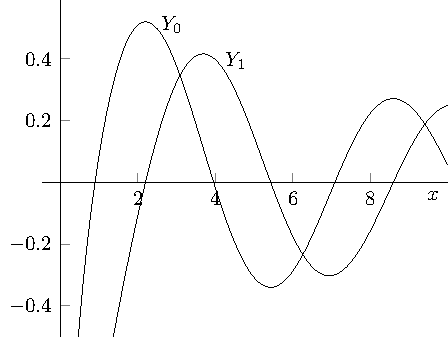
\includegraphics{figOctaveNeumannFunction}
\caption{بیسل تفاعل کے دوسرے اقسام۔}
\label{شکل_بیسل_نیومن_درجہ_صفر}
\end{figure}
جیسا شکل \حوالہ{شکل_بیسل_نیومن_درجہ_صفر} میں دکھایا گیا ہے کم قیمت کی مثبت \عددی{x} پر \عددی{Y_0} کی صورت \عددی{\ln x} کی طرح ہے اور \عددی{x\to \infty} پر \عددی{Y_0(x) \to \infty} ہو گا۔

\عددی{\nu=n=1,2,\cdots} کے لئے بھی بالکل اسی طرح، مساوات \حوالہ{مساوات_طاقتی_فروبنیوس_حل_ث} سے شروع کرتے ہوئے  دوسرا حل حاصل کیا جاتا ہے۔ان میں بھی لوگارتھمی جزو پایا جاتا ہے۔

دوسرے حل کا دارومدار اس حقیقت پر ہے کہ آیا \عددی{\nu} کا درجہ عدد صحیح ہے یا نہیں۔اس پیچیدگی  سے چھٹکارا حاصل کرنے کی خاطر دوسرے حل کو درج ذیل بیان کیا جاتا ہے جو تمام \عددی{\nu} کے لئے قابل استعمال ہے۔
\begin{gather}
\begin{aligned}\label{مساوات_بیسل_نیومن_عمومی_حل_الف}
Y_{\nu}(x)&=\frac{1}{\sin \nu \pi} [J_{\nu}(x)\cos \nu x-J_{-\nu}(x)] \quad \quad \text{(الف)}\\
Y_n(x)&=\lim_{\nu \to n} Y_{\nu}(x)\quad \quad \text{(ب)}
\end{aligned}
\end{gather}
درج بالا تفاعل کو \اصطلاح{درجہ \عددی{\nu} بیسل تفاعل کی دوسری قسم}\فرہنگ{بیسل تفاعل!دوسری قسم، درجہ \عددی{\nu}}\حاشیہب{Bessel function of the second kind of order $\nu$}\فرہنگ{Bessel function!second kind, order $\nu$} یا \اصطلاح{درجہ \عددی{\nu} نیومن تفاعل} کہتے ہیں۔ 

آئیں اب ثابت کریں کہ \عددی{J_{\nu}} اور \عددی{Y_{\nu}} تمام \عددی{\nu} اور تمام \عددی{x(>0)} کے لئے خطی طور غیر تابع ہیں۔

غیر عددی صحیح درجہ \عددی{\nu} کے لئے چونکہ \عددی{J_{\nu}(x)} اور \عددی{J_{-\nu}(x)} بیسل مساوات کے حل ہیں لہٰذا   \عددی{Y_{\nu}(x)} بھی بیسل مساوات کا حل ہے۔اب چونکہ ایسی \عددی{\nu} کے لئے \عددی{J_{\nu}(x)} اور \عددی{J_{-\nu}(x)} خطی طور غیر تابع ہیں اور \عددی{Y_{\nu}(x)} میں \عددی{J_{-\nu}(x)} پایا جاتا ہے لہٰذا \عددی{J_{\nu}(x)} اور \عددی{Y_{\nu}(x)} خطی طور غیر تابع ہوں گے۔مزید یہ کہ مساوات \حوالہ{مساوات_بیسل_نیومن_عمومی_حل_الف}-ب کو ثابت (صفحہ \حوالہصفحہ{حوالہ_بیرونی_مواد} پر حوالہ \cite{حوالہ_کریزگ_ب_اٹھارہ} میں ثبوت پیش کیا گیا ہے۔) کیا جا سکتا ہے لہٰذا عدد صحیح درجہ کے لئے \عددی{Y_n(x)} بیسل مساوات کا حل ہے۔آپ دیکھیں گے کہ \عددی{Y_n(x)} کی تسلسل میں لوگارتھمی جزو پایا جاتا ہے لہٰذا \عددی{J_n(x)} اور \عددی{Y_n(x)} خطی طور غیر تابع ہوں گے۔\عددی{Y_n(x)} کی تسلسل لکھنے کی خاطر \عددی{J_{\nu}(x)} کی تسلسل \حوالہ{مساوات_بیسل_تسلسل_عمومی} اور \عددی{J_{-\nu}(x)} کی تسلسل \حوالہ{مساوات_بیسل_تسلسل_عمومی_دوسرا} کو مساوات \حوالہ{مساوات_بیسل_نیومن_عمومی_حل_الف}-الف میں پر کرتے ہوئے \عددی{\nu \to n} کرتے ہیں (تفصیل صفحہ \حوالہصفحہ{حوالہ_بیرونی_مواد} پر \cite{حوالہ_کریزگ_ب_اٹھارہ} سے دیکھی جا سکتی ہے۔)
\begin{multline}\label{مساوات_بیسل_نیومن_عدد_صحیح_الف}
Y_n(x)=\frac{2}{\pi}J_n(x)\left(\ln \frac{x}{2}+\gamma\right)+\frac{x^n}{\pi}\sum_{m=0}^{\infty} \frac{(-1)^{m-1}(h_m+h_{m+n})}{2^{2m+n}m!(m+n)!}x^{2m}\\
-\frac{x^{-n}}{\pi}\sum_{m=0}^{n-1}\frac{(n-m-1)!}{2^{2m-n}m!}x^{2m}
\end{multline}
لکھا جا سکتا ہے جہاں \عددی{x>0} اور  \عددی{n=0,1,\cdots} جبکہ
\begin{align*}
h_0=0,\quad h_s=1+\frac{1}{2}+\frac{1}{3}+\cdots+\frac{1}{s} \quad \quad (s=1,2,\cdots)
\end{align*}
ہیں اور \عددی{n=0} کی صورت میں مساوات \حوالہ{مساوات_بیسل_نیومن_عدد_صحیح_الف} میں آخری مجموعے کی جگہ صفر لکھا جاتا ہے۔ درجہ صفر \عددی{n=0} پر  مساوات \حوالہ{مساوات_بیسل_نیومن_عدد_صحیح_الف} عین مساوات \حوالہ{مساوات_بیسل_نیومن_درجہ_صفر} کی صورت اختیار کرتی ہے۔اس کے علاوہ درج ذیل ثابت کیا جا سکتا ہے۔
\begin{align}
Y_{-n}(x)=(-1)^nY_n(x)
\end{align}
ان نتائج کو درج ذیل مسئلے میں پیش کرتے ہیں۔

%=======================
\ابتدا{مسئلہ} مساوات بیسل کا عمومی حل\\
تمام \عددی{\nu} کے لئے مساوات بیسل کا عمومی حل درج ذیل ہے۔
\begin{align}
y(x)=c_1J_{\nu}(x)+c_2Y_{\nu}(x)
\end{align}
\انتہا{مسئلہ}
%========================

بعض اوقات حقیقی \عددی{x} کے لئے مساوات بیسل کے مخلوط حل درکار ہوتے ہیں۔ایسی صورت میں درج ذیل خطی طور غیر تابع مخلوط حل  استعمال کیے جاتے ہیں جنہیں \اصطلاح{درجہ \عددی{\nu} بیسل تفاعل کی تیسری قسم}\فرہنگ{بیسل تفاعل!تیسری قسم}\حاشیہب{Bessel function of the third kind of order $\nu$}\فرہنگ{Bessel function!third kind} یا درجہ \عددی{\nu} پہلی اور دوسری \اصطلاح{ہینکل تفاعل}\فرہنگ{ہینکل تفاعل}\فرہنگ{تفاعل!ہینکل}\حاشیہب{Hankel functions}\فرہنگ{Hankel functions} کہا\حاشیہد{ہرمن ہینکل [1839-1873] جرمنی کے ریاضی دان۔} جاتا ہے۔
\begin{gather}
\begin{aligned}\label{مساوات_بیسل_ہینکل}
H_{\nu}^1(x)&=J_{\nu}(x)+iY_{\nu}(x)\\
H_{\nu}^2(x)&=J_{\nu}(x)-iY_{\nu}(x)
\end{aligned}
\end{gather}
%========================

\حصہء{سوالات}
سوال \حوالہ{سوال_بیسل_عمومی_حل_نیومن_الف} تا سوال \حوالہ{سوال_بیسل_عمومی_حل_نیومن_ب} کا عمومی حل \عددی{J_{\nu}} اور \عددی{Y_{\nu}} کی صورت میں حاصل کریں۔بتلائیں کہ کن سوالات میں \عددی{Y_{\nu}} کی جگہ \عددی{J_{-\nu}} استعمال کرنا ممکن ہے۔دی گئی اضافی معلومات استعمال کریں۔

%===============
\ابتدا{سوال}\شناخت{سوال_بیسل_عمومی_حل_نیومن_الف}\quad
$x^2y''+xy'+(x^2-25)y=0$\\
جواب:\عددی{y=c_1J_{5}(x)+c_2Y_{5}(x)}؛ چونکہ \عددی{\nu} عدد صحیح ہے لہٰذا \عددی{J_{-5}(x)} قابل استعمال نہیں ہے۔
\انتہا{سوال}
%=====================
\ابتدا{سوال}\quad
$x^2y''+xy'+(x^2-3)$\\
جواب:\عددی{y=c_1J_{\sqrt{3}}+c_2Y_{\sqrt{3}}(x)}؛ چونکہ \عددی{\nu} عدد صحیح نہیں ہے لہٰذا \عددی{J_{-\sqrt{3}}(x)} قابل استعمال ہے۔
\انتہا{سوال}
%===================
\ابتدا{سوال}\quad
$9x^2y''+9xy'+(z^{\tfrac{2}{3}}-\tfrac{9}{4})y=0, \quad \quad x=z^3$\\
جواب:\عددی{y=c_1J_{\tfrac{3}{2}}(x^{\tfrac{1}{3}})+c_2Y_{\tfrac{3}{2}}(x^{\tfrac{1}{3}})}
\انتہا{سوال}
%===================
\ابتدا{سوال}\quad
$x^2y''+xy'+(4x^4-\tfrac{16}{9})y=0,\quad \quad z=x^2$\\
جواب:\عددی{y=c_1J_{\tfrac{2}{3}}(x^2)+c_2Y_{\tfrac{2}{3}}(x^2)}
\انتہا{سوال}
%====================
\ابتدا{سوال}\quad
$9x^2y''+9xy'+(4x^{\tfrac{4}{3}}-25)y=0,\quad \quad z=x^{\tfrac{2}{3}}$\\
جواب:
$y=c_1J_{\tfrac{5}{2}}(x^{\tfrac{2}{3}})+c_2Y_{\tfrac{5}{2}}(x^{\tfrac{2}{3}})$
\انتہا{سوال}
%=================
\ابتدا{سوال}\quad
$y''+k^2x^2y=0,\quad \quad (y=u\sqrt{x},\quad z=\tfrac{kx^2}{2})$\\
جواب:\عددی{y=\sqrt{x}[c_1J_{\tfrac{1}{4}}(\tfrac{kx^2}{2})+c_2Y_{\tfrac{1}{4}}(\tfrac{kx^2}{2})]}
\انتہا{سوال}
%=================
\ابتدا{سوال}\quad
$xy''-5y'+xy=0,\quad \quad y=x^3u$\\
جواب:\عددی{y=x^3[c_1J_3(x)+c_2Y_3(x)]}
\انتہا{سوال}
%====================
\ابتدا{سوال}\quad
$xy''-y'+xy=0,\quad \quad y=xu$\\
جواب:\عددی{y=x[c_1J_1(x)+c_2Y_1(x)]}
\انتہا{سوال}
%=================
\ابتدا{سوال}\شناخت{سوال_بیسل_عمومی_حل_نیومن_ب}\quad
$xy''+5y'+xy=0,\quad \quad y=\tfrac{u}{x^2}$\\
جواب:\عددی{y=\tfrac{1}{x^2}[c_1J_2(x)+c_2Y_2(x)]}
\انتہا{سوال}
%===================
\ابتدا{سوال}\quad ترمیم شدہ درجہ \عددی{\nu} بیسل تفاعل کی پہلی قسم\\
ترمیم شدہ درجہ \عددی{\nu} بیسل تفاعل کی پہلی قسم کی تعریف \عددی{I_{\nu}(x)=i^{-\nu}J_{\nu}(ix)} ہے جہاں \عددی{i=\sqrt{-1}} ہے۔ثابت کریں  کہ \عددی{I_{\nu}(x)} درج ذیل تفرقی مساوات پر پورا اترتا ہے۔
\begin{align}\label{مساوت_بیسل_ترمیم_شدہ}
x^2y''+xy'-(x^2+\nu^2)y=0
\end{align}
جواب:\عددی{I_{\nu}(x)} کو دیے گئے مساوات میں پر کرتے ہوئے \عددی{0=0} حاصل کریں۔یہی ثبوت ہے۔
\انتہا{سوال}
%======================
\ابتدا{سوال}\quad ترمیم شدہ بیسل تفاعل\\
\عددی{I_{\nu}(x)} کی درج ذیل صورت حاصل کریں۔
\begin{align}
I_{\nu}(x)=\sum_{m=0}^{\infty}\frac{x^{2m+\nu}}{2^{2m+\nu}m!\Gamma(m+\nu+1)}
\end{align}
\انتہا{سوال}
%=======================
\ابتدا{سوال}\quad \عددی{I_{\nu}(x)} حقیقی ہے\\
ثابت کریں کہ حقیقی \عددی{x} اور حقیقی \عددی{\nu} کے لئے \عددی{I_{\nu}(x)} حقیقی ہے۔ثابت کریں کہ \عددی{x \ne 0} ہوتے ہوئے \عددی{I_{\nu}(x) \ne 0} ہو گا۔ ثابت کریں کہ \عددی{I_{-n}(x)=I_n(x)} کے برابر ہے جہاں \عددی{n} عدد صحیح ہے۔
\انتہا{سوال}
%====================
\ابتدا{سوال}\quad ترمیم شدہ بیسل تفاعل\\
ثابت کریں کہ تفاعل \عددی{K_{\nu}(x)}، جسے ترمیم شدہ بیسل تفاعل کی تیسری (بعض اوقات دوسری) قسم کہتے ہیں،
\begin{align}
K_{\nu}(x)=\frac{\pi}{2\sin \nu\pi}[I_{-\nu}(x)-I_{\nu}(x)]
\end{align}
تفرقی مساوات \حوالہ{مساوت_بیسل_ترمیم_شدہ} کا حل ہے۔ 
\انتہا{سوال}
%======================
\ابتدا{سوال}\quad ہینکل تفاعل\\
ثابت کریں کہ ہینکل تفاعل \حوالہ{مساوات_بیسل_ہینکل} مساوات بیسل کے حل کی اساس ہیں۔ 

\انتہا{سوال}
%==========================

\باب{لاپلاس تبادلہ}
لاپلاس بدل کی ترکیب سے ابتدائی قیمت (سرحدی قیمت) تفرقی مساوات حل کیے جاتے ہیں۔یہ ترکیب تین قدم پر مشتمل ہے۔
\begin{itemize}
\item
پہلا قدم: ابتدائی قیمت (سرحدی قیمت) تفرقی مساوات کا لاپلاس بدل لیتے ہوئے سادہ \اصطلاح{ضمنی مساوات} حاصل کی جاتی ہے۔
\item
دوسرا قدم:  ضمنی مساوات کو خالصتاً الجبرائی طور پر حل کیا جاتا ہے۔
\item
تیسرا قدم: ضمنی مساوات کے حل کا الٹ لاپلاس بدل لیتے ہوئے اصل حل حاصل کیا جاتا ہے۔
\end{itemize}  

یوں لاپلاس بدل تفرقی مساوات کے مسئلے کو سادہ الجبرائی مسئلہ میں تبدیل کرتا ہے۔تیسرے قدم پر الٹ لاپلاس بدل حاصل کرتے ہوئے عموماً ایسی جدول کا سہارا لیا جاتا ہے جس  میں تفاعل اور تفاعل کے الٹ لاپلاس بدل درج ہوں۔ 

انجینئری میں لاپلاس بدل کی ترکیب اہم کردار ادا کرتی ہے، بالخصوص ان مسائل میں جہاں جبری تفاعل غیر استمراری ہو، مثلاً جب جبری تفاعل کچھ وقفے کے لئے کار آمد ہو یا جبری تفاعل غیر سائن نما دہراتا تفاعل ہو۔

اب تک غیر متجانس مساوات کا عمومی حل حاصل کرتے ہوئے پہلے مطابقتی متجانس مساوات کا حل اور پھر غیر متجانس مساوات کا مخصوص حل حاصل کیا جاتا رہا۔لاپلاس بدل کی ترکیب میں عمومی حل ایک ہی بار میں حاصل ہوتا ہے۔اسی طرح لاپلاس بدل استعمال کرتے ہوئے ابتدائی قیمت (سرحدی قیمت) مسائل کے حل میں عمومی حل حاصل کرنے کے بعد ابتدائی (سرحدی) شرائط پر کرنے کی ضرورت پیش نہیں آتی چونکہ حل یہ شرائط شامل ہوتے ہیں۔
%=========================

\حصہ{لاپلاس بدل۔ الٹ لاپلاس بدل۔ خطیت}
فرض کریں کہ تفاعل \عددی{f(t)} تمام \عددی{t \ge 0} پر معین ہے۔ ہم \عددی{f(t)} کو \عددی{e^{-st}} سے ضرب دیتے ہوئے،  \عددی{t} کے ساتھ، \عددی{0} تا \عددی{\infty}، تکمل لیتے ہیں۔ اگر ایسا تکمل موجود ہو تو یہ \عددی{s} پر منحسر ہو گا لہٰذا اس کو \عددی{F(s)} لکھا جا سکتا ہے۔
\begin{align}
F(s)=\int_{0}^{\infty}e^{-st}f(t)\dif t
\end{align} 
تفاعل \عددی{F(s)} کو تفاعل \عددی{f(t)} کا \اصطلاح{لاپلاس بدل}\فرہنگ{لاپلاس بدل}\حاشیہب{ٔLaplace transform}\فرہنگ{Laplace transform} کہا جاتا ہے اور اس کو
 \عددی{\Laplace(f)} سے ظاہر کیا جاتا ہے۔
\begin{align}\label{مساوات_لاپلاس_بدل_الف}
F(s)=\Laplace(f)=\int_{0}^{\infty} e^{-st} f(t)\dif t
\end{align}
\عددی{f(t)} سے \عددی{F(s)} کے حصول کو \اصطلاح{لاپلاس تبادلہ}\فرہنگ{لاپلاس تبادلہ}\حاشیہب{Laplace transformation}\فرہنگ{Laplace transformation} کہتے ہیں۔

اسی طرح \عددی{f(t)} کو \عددی{F(s)} کا \اصطلاح{الٹ لاپلاس بدل}\فرہنگ{لاپلاس!الٹ بدل}\حاشیہب{inverse Laplace transform}\فرہنگ{Laplace!inverse transform} کہتے ہیں جسے \عددی{\Laplace^{-1}(F)} سے ظاہر کیا جاتا ہے۔
\begin{align}
f(t)=\Laplace^{-1}(F)
\end{align}

\موٹا{علامت نویسی}\\
اصل تفاعل کو چھوٹے لاطینی حرف تہجی سے ظاہر کیا جاتا ہے جبکہ لاپلاس بدل کو اسی حرف تہجی کی بڑی صورت سے ظاہر کیا جاتا ہے۔ یوں \عددی{f(t)} کا بدل \عددی{F(s)} ہو گا اور \عددی{g(t)} کا لاپلاس بدل \عددی{G(s)} ہو گا۔

%================
\ابتدا{مثال}
تفاعل \عددی{f(t)=1}، جہاں \عددی{t \ge 0} ہے، کا لاپلاس بدل مساوات \حوالہ{مساوات_لاپلاس_بدل_الف} سے بذریعہ تکمل حاصل کرتے ہیں۔
\begin{align*}
\Laplace(f)=\Laplace(1)=\int_{0}^{\infty} e^{-st} \dif t=\left. -\frac{1}{s}e^{-st}\right|_{0}^{\infty}
\end{align*}
ہو گا جو \عددی{s >0} کی صورت میں درج ذیل ہو گا۔
\begin{align*}
\Laplace(1)=\frac{1}{s}
\end{align*}
تکمل \حوالہ{مساوات_لاپلاس_بدل_الف} کی علامت پر آسائش ضرور ہے لیکن اس پر مزید غور کی ضرورت ہے۔اس تکمل کا وقفہ لامتناہی ہے۔ایسے تکمل کو \اصطلاح{غیر مناسب تکمل}\فرہنگ{غیر مناسب تکمل}\حاشیہب{improper integral}\فرہنگ{improper integral} کہتے ہیں اور حزب  تعریف، اس کی قیمت درج ذیل اصول کے تحت حاصل کی جاتی ہے۔ 
\begin{align*}
\int_{0}^{\infty} e^{-st}f(t)\dif t=\lim_{T\to \infty} \int_{0}^{T}e^{-st}f(t)\dif t
\end{align*}
یوں اس مثال میں اس آسائش علامت کا مطلب درج ذیل ہے۔
\begin{align*}
\int_{0}^{\infty}e^{-st}\dif t=\lim_{T\to \infty}\int_{0}^{T}e^{-st}\dif t=\lim_{T\to \infty}\left[-\frac{1}{s}e^{-sT}+\frac{1}{s}e^{0}\right]=\frac{1}{s}, \quad (s>0)
\end{align*}
اس پورے باب میں تکمل کی یہی علامت استعمال کی جائے گی۔
\انتہا{مثال}
%=================
\ابتدا{مثال}\شناخت{مثال_لاپلاس_قوت_نمائی_الف}
تفاعل \عددی{f(t)=e^{at}} جہاں \عددی{t \ge 0} اور \عددی{a} مستقل ہے کا لاپلاس بدل \عددی{\Laplace(f)} دریافت کریں۔

حل:مساوات \حوالہ{مساوات_لاپلاس_بدل_الف} سے
\begin{align*}
\Laplace(e^{at})=\int_{0}^{\infty} e^{-st}e^{at}\dif t=\left.\frac{1}{a-s}e^{-(s-a)t} \right|_{0}^{\infty}
\end{align*}
ملتا ہے۔اب اگر \عددی{s-a >0} ہو (یعنی \عددی{s} کی قیمت \عددی{a} سے زیادہ چننی گئی ہو۔)  تب درج ذیل حاصل ہو گا۔
\begin{align*}
\Laplace(e^{at})=\frac{1}{s-a}
\end{align*}
\انتہا{مثال}
%=================

اگرچہ ہم بالکل اسی طرز پر دیگر تفاعل کے لاپلاس بدل بذریعہ تکمل حاصل کر سکتے ہیں، حقیقت میں لاپلاس تبادلہ کے ایسی کئی خواص ہیں جنہیں استعمال کرتے ہوئے دیگر لاپلاس بدل نہایت عمدگی کے ساتھ حاصل کیے جا سکتے ہیں۔لاپلاس تبادلہ کی ایک خاصیت  خطیت ہے جس سے مراد درج ذیل ہے۔
%================

\ابتدا{مسئلہ}\شناخت{مسئلہ_لاپلاس_خطیت}\quad لاپلاس تبادلہ کی خطیت\\
لاپلاس تبادلہ خطی عمل ہے۔یوں ایسے تفاعل \عددی{f(t)} اور \عددی{g(t)}، جن کے لاپلاس بدل موجود ہوں، کے عمومی مجموعے کا لاپلاس بدل درج ذیل ہو گا جہاں \عددی{a} اور \عددی{b} مستقل ہیں۔
\begin{align*}
\Laplace[af(t)+bg(t)]=a\Laplace[f(t)]+b\Laplace[g(t)]
\end{align*}
\انتہا{مسئلہ}
%=================
\ابتدا{ثبوت}
لاپلاس تبدلہ کی تعریف سے درج ذیل لکھتے ہیں۔
\begin{align*}
\Laplace[af(t)+bg(t)]&=\int_{0}^{\infty}e^{-st}[af(t)+bg(t)]\dif t\\
&=a\int_{0}^{\infty}e^{-st}f(t)\dif t+b\int_{0}^{\infty}e^{-st}g(t) \dif t\\
&=a\Laplace[f(t)]+b\Laplace[g(t)]
\end{align*}
\انتہا{ثبوت}
%=====================

\ابتدا{مثال}
آئیں تفاعل \عددی{f(t)=\cosh at} کا لاپلاس بدل مسئلہ \حوالہ{مسئلہ_لاپلاس_خطیت} اور مثال \حوالہ{مثال_لاپلاس_قوت_نمائی_الف} کی مدد سے لکھیں۔
 چونکہ \عددی{\cosh at=\tfrac{1}{2}(e^{at}+e^{-at})} ہے لہٰذا 
\begin{align*}
\Laplace(\cosh at)=\frac{1}{2}\Laplace(e^{at})+\frac{1}{2}\Laplace(e^{-at})=\frac{1}{2}\left(\frac{1}{s-a}+\frac{1}{s+a}\right)=\frac{s}{s^2-a^2}
\end{align*}
ہو گا جہاں \عددی{s>a\ge 0} چننا گیا ہے۔
\انتہا{مثال}
%=======================
\ابتدا{مثال}
آئیں تفاعل \عددی{\sinh at} کا لاپلاس بدل حاصل کریں۔چونکہ \عددی{\sinh at=\tfrac{1}{2}(e^{at}-e^{{-at}})} ہے لہٰذا مسئلہ خطیت سے تفاعل کا لاپلاس بدل درج ذیل ہو گا۔
\begin{align*}
\Laplace(\sinh at)=\frac{1}{2}\Laplace(e^{at})-\frac{1}{2}\Laplace(e^{-at})=\frac{1}{2}\left(\frac{1}{s-a}-\frac{1}{s+a}\right)=\frac{a}{s^2-a^2}
\end{align*}
\انتہا{مثال}
%=========================
\ابتدا{مثال}
\عددی{\cos \omega t} اور \عددی{\sin \omega t} کے لاپلاس بدل حاصل کریں۔

حل:انہیں \عددی{\cos \omega t=\tfrac{1}{2}(e^{j\omega t}+e^{-j\omega t})} اور \عددی{\sin \omega t=\tfrac{1}{2j}(e^{j\omega t}-e^{-j\omega t})} لکھ کر لاپلاس بدل حاصل کرتے ہیں۔
\begin{align*}
\Laplace(\cos \omega t)&=\frac{1}{2}\Laplace(e^{j\omega t})+\frac{1}{2}\Laplace(e^{-j\omega t})=\frac{1}{2}\left(\frac{1}{s-j\omega}+\frac{1}{s+j\omega}\right)=\frac{s}{s^2+\omega^2}\\
\Laplace(\sin \omega t)&=\frac{1}{2j}\Laplace(e^{j\omega t})-\frac{1}{2j}\Laplace(e^{-j\omega t})=\frac{1}{2j}\left(\frac{1}{s-j\omega}-\frac{1}{s+j\omega}\right)=\frac{\omega}{s^2+\omega^2}
\end{align*}
\انتہا{مثال}
%===========================
جدول \حوالہ{جدول_لاپلاس_بدل_الف} میں چند اہم بنیادی تفاعل اور ان کے لاپلاس بدل دیے گئے ہیں۔اس جدول میں دیے لاپلاس بدل جاننے کے بعد ہم تقریباً ان تمام تفاعل کے بدل، لاپلاسی خواص سے حاصل کر پائیں گے،  جو ہمیں درکار ہوں گے۔
\begin{table}
\caption{چند بنیادی تفاعل \عددی{f(t)} اور ان کے لاپلاس بدل \عددی{\Laplace(f)}}
\label{جدول_لاپلاس_بدل_الف}
\centering
\begin{tabular}{ccc| ccc}
 شمار& $f(t)$& $\Laplace(f)$& شمار& $f(t)$& $\Laplace(f)$\\[0.5ex]
\hline
$1$&$1$&$\frac{1}{s}$&$7$&$\cos \omega t$&$\frac{s}{s^2+\omega^2}$\Tstrut\\[1ex]
$2$&$t$&$\frac{1}{s^2}$&$8$&$\sin \omega t$&$\frac{\omega}{s^2+\omega^2}$\\[1ex]
$3$&$t^2$&$\frac{2!}{s^3}$&$9$&$\cosh at$&$\frac{s}{s^2-a^2}$\\[1ex]
$4$&\shortstack{$t^n$\\ ($n=1,2,\cdots$)}&$\frac{n!}{s^{n+1}}$&$10$&$\sinh at$&$\frac{a}{s^2-a^2}$\\[1ex]
$5$&\shortstack{$t^a$\\($ a>0$)}&$\frac{\Gamma(a+1)}{s^{a+1}}$&$11$& $e^{at}\cos \omega t$& $\frac{s-a}{(s-a)^2+\omega^2}$\\[1.5ex]
$6$& $e^{at}$&$\frac{1}{s-a}$&$12$& $e^{at}\sin \omega t$& $\frac{\omega}{(s-a)^2+\omega^2}$
\end{tabular}
\end{table}

جدول \حوالہ{جدول_لاپلاس_بدل_الف} میں پہلا، دوسرا اور تیسرا کلیہ چوتھے کلیے سے اخذ کیے جا سکتے ہیں جبکہ چوتھا کلیہ از خود پانچویں کلیہ میں مساوات \حوالہ{مساوات_بیسل_گیما_بطور_عدد_ضربیہ} استعمال کرتے ہوئے \عددی{\Gamma(n+1)=n!} لکھ کر حاصل کیا جا سکتا ہے، جہاں \عددی{n} غیر منفی \عددی{n \ge 0} عدد صحیح ہے۔ پانچواں کلیہ، لاپلاس بدل کی تعریف مساوات \حوالہ{مساوات_لاپلاس_بدل_الف}
\begin{align*}
\Laplace(t^a)=\int_{0}^{\infty}e^{-st}t^a\dif t
\end{align*}
میں \عددی{st=x} پر کرتے ہوئے مساوات \حوالہ{مساوات_بیسل_گیما_الف} کے استعمال سے حاصل کرتے ہیں۔
\begin{align*}
\Laplace(t^a)=\int_{0}^{\infty}e^{-x}\left(\frac{x}{s}\right)^a \frac{\dif x}{s}=\frac{1}{s^{a+1}}\int_{0}^{\infty}e^{-x}x^a\dif x=\frac{\Gamma(a+1)}{s+1},\quad \quad (s>0)
\end{align*}
%============================

\جزوحصہء{\عددی{s} منتقلی}
تفاعل \عددی{f(t)}  کا لاپلاس بدل جانتے ہوئے تفاعل \عددی{e^{at}f(t)} کا لاپلاس بدل درج ذیل مسئلہ کی مدد سے فوراً لکھا جا سکتا ہے۔

%=============
\ابتدا{مسئلہ}\شناخت{مسئلہ_لاپلاس_بدل_قوت_نمائی}\quad منتقلی کا پہلا مسئلہ، \عددی{s} منتقلی\\
اگر تفاعل \عددی{f(t)} کا لاپلاس بدل \عددی{F(s)} ہو (جہاں کسی \عددی{k} کے لئے \عددی{s>k} ہے) تب تفاعل \عددی{e^{at}f(t)} کا لاپلاس بدل \عددی{F(s-a)} ہو گا (جہاں \عددی{s-a>k} ہے)۔
\begin{align*}
\Laplace[e^{at}f(t)]=F(s-a)
\end{align*}
اس مساوات کو الٹ لاپلاس بدل کی صورت میں بھی لکھا جا سکتا ہے یعنی
\begin{align*}
e^{at}f(t)=\Laplace^{-1}[F(s-a)]
\end{align*}
\انتہا{مسئلہ}
%=======================

\ابتدا{ثبوت}
لاپلاس بدل کے تکمل مساوات \حوالہ{مساوات_لاپلاس_بدل_الف} میں \عددی{s} کی جگہ \عددی{s-a} پر کرتے ہوئے 
\begin{align}\label{}
F(s-a)=\int_{0}^{\infty} e^{-(s-a)t} f(t)\dif t=\int_{0}^{\infty}e^{-st}{e^{at}f(t)}\dif t=\Laplace[e^{at}f(t)]
\end{align}
ملتا ہے۔اگر کسی \عددی{s>k} کے لئے \عددی{F(s)} موجود ہو یعنی اس کی قیمت محدود ہو تب \عددی{s-a>k} کے لئے پہلا تکمل بھی موجود ہو گا (یعنی محدود قیمت کا ہو گا)۔ اس کلیے کے دونوں اطراف کا الٹ لاپلاس بدل لینے سے مسئلے کی دوسری مساوات حاصل ہوتی ہے۔
\انتہا{ثبوت}
%======================

\ابتدا{مثال}\شناخت{مثال_لاپلاس_بدل_قصری_ارتعاش}\quad قصری ارتعاش\\
جدول \حوالہ{جدول_لاپلاس_بدل_الف} میں \عددی{\cos \omega t} اور \عددی{\sin \omega t} کے بدل کو استعمال کرتے ہوئے جدول میں گیارہ اور بارہ شمار پر دیے گئے لاپلاس بدل کو مسئلہ \حوالہ{مسئلہ_لاپلاس_بدل_قوت_نمائی} کی مدد سے فوراً لکھا جا سکتا ہے۔
\begin{align*}
\Laplace[e^{at}\cos \omega t]=\frac{s-a}{(s-a)^2+\omega^2} \quad \quad \Laplace[e^{at}\sin \omega t]=\frac{\omega}{(s-a)^2+\omega^2}
\end{align*}
انہیں استعمال کرتے ہوئے درج ذیل کا الٹ لاپلاس بدل حاصل کریں۔
\begin{align*}
\Laplace(f)=\frac{4s+24}{s^2+2s+101}
\end{align*}
حل:اس کو درکار صورت
\begin{align*}
f=\Laplace^{-1}\left[\frac{4(s+1)+2(10)}{(s+1)^2+10^2}\right]=4\Laplace^{-1}\left[\frac{s+1}{(s+1)^2+10^2}\right]+2\Laplace^{-1}\left[\frac{10}{(s+1)^2+10^2}\right]
\end{align*}
 میں لاتے ہوئے الٹ لاپلاس بدل لکھتے ہیں
\begin{align*}
f=e^{-t}(4\cos 10t+2\sin 10t)
\end{align*}
 جسے شکل \حوالہ{شکل_لاپلاس_قصری_ارتعاش} میں دکھایا گیا ہے۔یہ قصری ارتعاش کو ظاہر کرتی ہے۔
\begin{figure}
\centering
\begin{tikzpicture}
\begin{axis}[small,axis lines*=middle,xlabel={$t$},xlabel style={at={(current axis.right of origin)},anchor=north east}]
\addplot[domain=0:3,samples=150]{e^(-x)*(4*cos(180/pi*10*x)+2*sin(180/pi*10*x))};
\end{axis}
\end{tikzpicture}
\caption{قصری ارتعاش (مثال \حوالہ{مثال_لاپلاس_بدل_قصری_ارتعاش})}
\label{شکل_لاپلاس_قصری_ارتعاش}
\end{figure}
\انتہا{مثال}
%=======================

\جزوحصہء{لاپلاس بدل کی وجودیت اور یکتائی}
اگر تمام  \عددی{t \ge 0} کے لئے، کسی مستقل \عددی{k} اور \عددی{M} پر تفاعل \عددی{f} \موٹا{بڑھنے کی پابندی}
\begin{align}\label{مساوات_لاپلاس_بڑھنے_کی_حد}
\abs{f(t)} \le M e^{kt}
\end{align}
پر پورا اترتا ہو، تب اس کا لاپلاس بدل موجود ہو گا۔ہم کہتے ہیں کہ نہایت تیزی سے نہ بڑھنے والے  تفاعل \عددی{f(t)} کا لاپلاس بدل موجود ہو گا۔

\عددی{f(t)} کا استمراری  ہونا ضروری نہیں ہے البتہ اس کا \اصطلاح{ٹکڑوں میں استمراری}\فرہنگ{استمراری!ٹکڑوں میں}\حاشیہب{piecewise continuous}\فرہنگ{continuous!piecewise} ہونا لازم ہے۔  اگر محدود وقفہ \عددی{a \le t \le b} جس پر \عددی{f(t)} معین ہو، کو کئی ایسے ٹکڑوں میں تقسیم کرنا ممکن ہو کہ ہر ٹکڑے پر \عددی{f(t)} استمراری ہو اور \عددی{t} کا اندرون ٹکڑے سے ٹکڑے کے (دونوں) سروں تک پہنچنے پر  \عددی{f(t)} کی قیمت کا \اصطلاح{حد}\حاشیہب{limit} محدود حاصل ہو تب \عددی{f(t)} \اصطلاح{ٹکڑوں میں استمراری} کہلائے گا۔ ایسی صورت میں، جیسا شکل \حوالہ{شکل_لاپلاس_ٹکڑوں_استمراری} میں دکھایا گیا ہے، محدود \اصطلاح{چھلانگ}\فرہنگ{چھلانگ}\حاشیہب{jumps}\فرہنگ{jumps} پائے جائیں گے جو غیر استمراری صورت کی واحد وجہ ہو گی۔ عموماً عملی مسائل اسی نوعیت کے ہوتے ہیں۔درج ذیل مسئلہ بھی اسی نوعیت کا ہے۔ 
\begin{figure}
\centering
\begin{tikzpicture}
%axis
\draw(0,-1)--(0,2);
\draw(0,0)--++(6,0)node[right]{$t$};
\draw(1,0)--++(0,-0.1)node[below]{$a$};
\draw(5,0)--++(0,-0.1)node[below]{$b$};
%piecewise continuous
\draw(1,0.5) to [out=30,in=-150]++(1,1)node[circ]{};
\draw(2,2) to [out=-20,in=120]++(1,-2.5)node[circ]{};
\draw(3,0.3) to [out=0,in=-145]++(1,0.5)coordinate(kA);
\draw(4,1.4)coordinate(kB)--++(0.4,0)--++(0.6,-0.5);
\draw($(kA)!0.5!(kB)$) node[circ]{};
\end{tikzpicture}
\caption{ٹکڑوں میں استمراری تفاعل \عددی{f(t)}۔ غیر استمراری مقام پر تفاعل کی قیمت کو نقطوں سے ظاہر کیا گیا ہے۔}
\label{شکل_لاپلاس_ٹکڑوں_استمراری}
\end{figure}
%=============

\ابتدا{مسئلہ}\شناخت{مسئلہ_لاپلاس_وجودیت}\quad مسئلہ وجودیت لاپلاس بدل\\
اگر نصف محور \عددی{t \ge 0} کے ہر محدود وقفے پر تفاعل \عددی{f(t)} معین اور ٹکڑوں میں استمراری ہو اور مساوات \حوالہ{مساوات_لاپلاس_بڑھنے_کی_حد} پر، 
تمام \عددی{t \ge 0} اور کسی مستقل \عددی{M} اور \عددی{k} کے لئے،  پورا اترتا ہو تب لاپلاس بدل \عددی{\Laplace (f)} تمام \عددی{s >k} کے لئے موجود ہو گا ۔ 
\انتہا{مسئلہ}
%=========================

\ابتدا{ثبوت}
چونکہ \عددی{f(t)} ٹکڑوں میں استمراری ہے لہٰذا \عددی{t} محور کے کسی بھی محدود وقفے پر \عددی{e^{-st}f(t)} قابل تکمل ہے۔ مساوات \حوالہ{مساوات_لاپلاس_بڑھنے_کی_حد} کو دیکھ کر، \عددی{s>k} تصور کرتے ہوئے (جو درج ذیل آخری تکمل میں درکار ہے)، لاپلاس بدل کی وجودیت کا ثبوت حاصل کرتے ہیں۔
\begin{align*}
\abs{\Laplace(f)} = \abs{\int_{0}^{\infty} e^{-st}f(t)\dif t}\le \int_{0}^{\infty} \abs{f(t)}e^{-st}\dif t\le \int_{0}^{\infty} Me^{kt}e^{-st}\dif t=\frac{M}{s-k}
\end{align*}
\انتہا{ثبوت}
%=========================

کسی بھی تفاعل کا مساوات \حوالہ{مساوات_لاپلاس_بڑھنے_کی_حد} میں دیے گئے شرط پر پورا اترنے کو با آسانی دیکھا جا سکتا ہے، مثلاً \عددی{\cosh t < e^t} یا \عددی{t^n<n!e^t} (چونکہ \عددی{\tfrac{t^n}{n!}} مکلارن تسلسل کا ایک رکن ہے)۔ ایسا تفاعل جو مساوات \حوالہ{مساوات_لاپلاس_بڑھنے_کی_حد} پر پورا نہ اترتا ہو کی مثال \عددی{e^{t^2}} ہے۔آپ سوال \حوالہ{سوال_لاپلاس_کافی} میں دیکھیں گے کہ مسئلہ \حوالہ{مسئلہ_لاپلاس_وجودیت} میں دیے گئے شرائط لاپلاس بدل کی وجودیت کے لئے کافی ہیں نا کہ لازمی ہیں۔

\جزوحصہء{یکتائی}
اگر کسی تفاعل کا لاپلاس بدل موجود ہو تو یہ بدل یکتا ہو گا۔اسی طرح اگر (حقیقی مثبت محور پر معین) دو تفاعل کے لاپلاس بدل یکساں ہوں تب یہ تفاعل، کسی بھی مثبت لمبائی کے وقفے پر،  آپس میں مختلف نہیں ہو سکتے ہیں، البتہ تنہا نقطوں پر ان کی قیمت غیر یکساں ہو سکتی ہے۔یوں ہم کہہ سکتے ہیں کہ الٹ لاپلاس بدل یکتا ہے۔ بالخصوص دو ایسے استمراری تفاعل جن کا لاپلاس بدل یکساں ہو، آپس میں مکمل طور پر یکساں ہوں گے۔ 
%========================

\حصہء{سوالات}
%=============
سوال \حوالہ{سوال_لاپلاس_بدل_الف} تا سوال \حوالہ{سوال_لاپلاس_بدل_ب} میں لاپلاس بدل حاصل کریں۔ \عددی{a} اور  \عددی{b} کو مستقل تصور کریں۔

\ابتدا{سوال}\شناخت{سوال_لاپلاس_بدل_الف}\quad
$2t-3$\\
جواب:\عددی{\tfrac{2}{s^2}-\tfrac{3}{s}}
\انتہا{سوال}
%=======================
\ابتدا{سوال}\quad
$(at+b)^2$\\
جواب:\عددی{a(\tfrac{b}{s^2}+\tfrac{2a}{s^3})+b(\tfrac{b}{s}+\tfrac{a}{s^2})}
\انتہا{سوال}
%=====================
\ابتدا{سوال}\quad
$\sin 2\pi t$\\
جواب:\عددی{\tfrac{2\pi}{s^2+4\pi^2}}
\انتہا{سوال}
%====================
\ابتدا{سوال}\quad
$\sin^2 2\pi t$\\
جواب:\عددی{\tfrac{8\pi^2}{s(s^2+16\pi^2)}}
\انتہا{سوال}
%====================
\ابتدا{سوال}\quad
$e^{-3t}\sin 4t$\\
جواب:\عددی{\tfrac{4}{(s+3)^2+16}}
\انتہا{سوال}
%======================
\ابتدا{سوال}\quad
$e^{2t}\cos 3t$\\
جواب:\عددی{\tfrac{s-2}{(s-2)^2+9}}
\انتہا{سوال}
%======================
\ابتدا{سوال}\quad
$\cos (2t-\frac{\pi}{3})$\\
جواب:\عددی{\tfrac{\tfrac{s}{2}+\sqrt{3}}{s^2+4}}
\انتہا{سوال}
%=========================
\ابتدا{سوال}\شناخت{سوال_لاپلاس_بدل_ب} \quad
$2\sin (5t+\pi)$\\
جواب:\عددی{\tfrac{-10}{s^2+25}}
\انتہا{سوال}
%======================
\begin{figure}
\centering
\begin{subfigure}{0.33\textwidth}
\centering
\begin{tikzpicture}
%axis
\draw[gray](0,0)--(0,1.5);
\draw[gray](0,0)--(3,0);
%function
\draw[thick](0,0)--(2,1);
\draw[dashed](2,1)--(2,0);
\draw[thick](2,0)node[below]{$2$}--(3,0);
\draw(0,1)--++(-0.1,0)node[left]{$1$};
\draw(1,-0.5)node{(الف)};
\end{tikzpicture}%
\end{subfigure}%
\begin{subfigure}{0.33\textwidth}
\centering
\begin{tikzpicture}
%axis
\draw[gray](0,0)--(0,1.5);
\draw[gray](0,0)--(3,0);
%function
\draw[thick](0,1)--(2,1);
\draw[dashed](2,1)--(2,0)node[below]{$3$};
\draw[thick](2,0)--(3,0);
\draw(0,1)--++(-0.1,0)node[left]{$2$};
\draw(1,-0.5)node{(ب)};
\end{tikzpicture}%
\end{subfigure}%
\begin{subfigure}{0.33\textwidth}
\centering
\begin{tikzpicture}
%axis
\draw[gray](0,0)--(0,1.5);
\draw[gray](0,0)--(3,0);
%function
\draw[thick](0,1)--(2,0);
\draw[thick](2,0)node[below]{$5$}--(3,0);
\draw(0,1)--++(-0.1,0)node[left]{$2$};
\draw(1,-0.5)node{(پ)};
\end{tikzpicture}%
\end{subfigure}
%
\begin{subfigure}{0.33\textwidth}
\centering
\begin{tikzpicture}
%axis
\draw[gray](0,-1.2)--(0,1.2);
\draw[gray](0,0)--(3,0);
%function
\draw[thick](0,1)--(2,-1);
\draw[dashed](2,-1)--(2,0);
\draw[thick](2,0)node[above]{$2$}--(3,0);
\draw(0,1)--++(-0.1,0)node[left]{$5$};
\draw(0,-1)--++(-0.1,0)node[left]{$-5$};
\draw(0.75,-0.75)node{(ت)};
\end{tikzpicture}%
\end{subfigure}%
\begin{subfigure}{0.33\textwidth}
\centering
\begin{tikzpicture}
%axis
\draw[gray](0,0)--(0,1.5);
\draw[gray](0,0)--(3,0);
%function
\draw[thick](0,0)--(1,1)--(2.5,0)node[below]{$7$}--(3,0);
\draw(0,1)--++(-0.1,0)node[left]{$2$};
\draw(1,0)--++(0,-0.1)node[below]{$3$};
\draw(1,-0.75)node{(ٹ)};
\end{tikzpicture}%
\end{subfigure}%
\begin{subfigure}{0.33\textwidth}
\centering
\begin{tikzpicture}
%axis
\draw[gray](0,0)--(0,1.5);
\draw[gray](0,0)--(3,0);
%function
\draw[thick](0,0)--(1,1);
\draw[dashed](1,1)--(1,1.5);
\draw[thick](1,1.5)--(2,1.5);
\draw[dashed](2,1.5)--(2,0);
\draw[thick](2,0)node[below]{$4$}--(3,0);
\draw(0,1)--++(-0.1,0)node[left]{$2$};
\draw(0,1.5)--++(-0.1,0)node[left]{$3$};
\draw(1,0)--++(0,-0.1)node[below]{$2$};
\draw(1.5,-0.75)node{(ث)};
\end{tikzpicture}%
\end{subfigure}
\caption{سوال \حوالہ{سوال_لاپلاس_بدل_پ} تا سوال \حوالہ{سوال_لاپلاس_بدل_پ} کے اشکال۔}
\label{شکل_سوال_لاپلاس_بدل_پ}
\end{figure}
%================
\ابتدا{سوال}\شناخت{سوال_لاپلاس_بدل_پ} 
شکل \حوالہ{شکل_سوال_لاپلاس_بدل_پ}-الف میں ٹکڑوں میں استمراری تفاعل دکھایا گیا ہے۔تمام ٹکڑوں کی ریاضی مساوات حاصل کریں۔ تکمل \حوالہ{مساوات_لاپلاس_بدل_الف}  کو ٹکڑوں میں تقسیم کرتے ہوئے لاپلاس بدل حاصل کریں۔

جواب:\عددی{\tfrac{1-e^{-2s}(2s+1)}{2s^2}}
\انتہا{سوال}
%=========================
\ابتدا{سوال}
شکل \حوالہ{شکل_سوال_لاپلاس_بدل_پ}-ب میں دیے گئے تفاعل کا لاپلاس بدل حاصل کریں۔

جواب:\عددی{\tfrac{2}{s}(1-e^{-3s})}
\انتہا{سوال}
%===========================
\ابتدا{سوال}
شکل \حوالہ{شکل_سوال_لاپلاس_بدل_پ}-پ میں دیے گئے تفاعل کا لاپلاس بدل حاصل کریں۔

جواب:\عددی{\tfrac{2e^{-5s}+10s-2}{5s^2}}
\انتہا{سوال}
%===========================
\ابتدا{سوال}
شکل \حوالہ{شکل_سوال_لاپلاس_بدل_پ}-ت میں دیے گئے تفاعل کا لاپلاس بدل حاصل کریں۔

جواب:\عددی{\tfrac{5(s+1)e^{-2s}+5(s-1)}{s^2}}
\انتہا{سوال}
%===========================
\ابتدا{سوال}
شکل \حوالہ{شکل_سوال_لاپلاس_بدل_پ}-ٹ میں دیے گئے تفاعل کا لاپلاس بدل حاصل کریں۔

جواب:\عددی{\tfrac{4-7e^{-3s}+3e^{-7s}}{6s^2}}
\انتہا{سوال}
%===========================
\ابتدا{سوال}
شکل \حوالہ{شکل_سوال_لاپلاس_بدل_پ}-ث میں دیے گئے تفاعل کا لاپلاس بدل حاصل کریں۔

جواب:\عددی{\tfrac{1+(s-1)e^{-2s}-3se^{-4s}}{s^2}}
\انتہا{سوال}
%===========================
\ابتدا{سوال}\شناخت{سوال_لاپلاس_کافی}\quad وجودیت\\
تفاعل \عددی{\tfrac{1}{\sqrt{t}}} کا لاپلاس بدل حاصل کریں۔ایسا کرتے ہوئے \عددی{\Gamma(\tfrac{1}{2})=\sqrt{\pi}} (مساوات \حوالہ{مساوات_بیسل_گیما_نیم}) کا استعمال کریں۔ اس سے آپ اخذ کر سکتے ہیں کہ مسئلہ \حوالہ{مسئلہ_لاپلاس_وجودیت} میں دیے شرائط کافی ہیں نا کہ لازمی۔

جواب:\عددی{\tfrac{\sqrt{\pi}}{s}}
\انتہا{سوال}
%==============================
\ابتدا{سوال}
\عددی{e^{at}} کا لاپلاس بدل \عددی{\cosh at} اور \عددی{\sinh at} کے لاپلاس بدل سے حاصل کریں۔

جواب:\عددی{e^{at}=\sinh at+\cosh at} لکھ کر جواب \عددی{\tfrac{1}{s-a}} ملتا ہے۔
\انتہا{سوال}
%============================
\ابتدا{سوال}\quad پیمائشی فیتہ میں ردوبدل\\
ثابت کریں کہ اگر \عددی{\Laplace[f(t)]=F(s)}  ہو تب \عددی{\Laplace[f(ct)]=\tfrac{F(\tfrac{s}{c})}{c}} ہو گا جہاں \عددی{c} مستقل ہے۔اس کلیے کو استعمال کرتے ہوئے \عددی{\Laplace(\cos t)} سے \عددی{\Laplace(\cos \omega t)} حاصل کریں۔

جواب:مساوات \حوالہ{مساوات_لاپلاس_بدل_الف} استعمال کرتے ہوئے کلیہ ثابت ہو گا۔
\انتہا{سوال}
%=============================
\ابتدا{سوال}\quad الٹ لاپلاس بدل کی خطیت\\
\عددی{\Laplace} کی خطیت کو استعمال کرتے ہوئے ثابت کریں کہ \عددی{\Laplace^{-1}} خطی ہے۔
\انتہا{سوال}
%==============================
سوال \حوالہ{سوال_لاپلاس_الٹ_الف} تا سوال \حوالہ{سوال_لاپلاس_الٹ_ب} میں الٹ لاپلاس بدل حاصل کریں۔

%==============
\ابتدا{سوال}\شناخت{سوال_لاپلاس_الٹ_الف}\quad
$\frac{0.5s+1.3}{s^2+1.69}$\\
جواب:\عددی{\sin (1.3t)+0.5\cos(1.3t)}
\انتہا{سوال}
%========================
\ابتدا{سوال}\quad
$\frac{4s+1}{s^2-16}$\\
جواب:\عددی{\tfrac{1}{8}(17e^{4t}+15e^{-4t})}
\انتہا{سوال}
%========================
\ابتدا{سوال}\quad
$\frac{s}{m^2s^2+n^2}$\\
جواب:\عددی{\tfrac{\cos \tfrac{nt}{m}}{m^2}}
\انتہا{سوال}
%=========================
\ابتدا{سوال}\quad
$\frac{1}{(s+3)(s-2)}$\\
جواب:\عددی{\tfrac{1}{5}(e^{2t}-e^{-3t})}
\انتہا{سوال}
%========================
\ابتدا{سوال}\quad
$\frac{2}{s^3}+\frac{3}{s^5}$\\
جواب:\عددی{t^2+\tfrac{t^4}{8}}
\انتہا{سوال}
%======================
\ابتدا{سوال}\quad
$\frac{3s+8}{s^2-9}$\\
جواب:\عددی{\tfrac{1}{6}(17e^{3t}+e^{-3t})}
\انتہا{سوال}
%========================
\ابتدا{سوال}\quad
$\frac{s-1}{s^2-s-6}$\\
جواب:\عددی{\tfrac{1}{5}(2e^{3t}+3e^{-2t})}
\انتہا{سوال}
%=======================
\ابتدا{سوال}\شناخت{سوال_لاپلاس_الٹ_ب}\quad
$\frac{1}{(s-a)(s+b)}$\\
جواب:\عددی{\tfrac{1}{a+b}(e^{at}-e^{-bt})}
\انتہا{سوال}
%=====================
سوال \حوالہ{سوال_لاپلاس_منتقلی_الف} تا سوال \حوالہ{سوال_لاپلاس_منتقلی_ت} منتقلی \عددی{s} پر مبنی ہیں۔ سوال \حوالہ{سوال_لاپلاس_منتقلی_الف} تا سوال \حوالہ{سوال_لاپلاس_منتقلی_ب} میں لاپلاس بدل جبکہ سوال \حوالہ{سوال_لاپلاس_منتقلی_پ} تا سوال \حوالہ{سوال_لاپلاس_منتقلی_ت} میں الٹ لاپلاس بدل حاصل کریں۔

%=========
\ابتدا{سوال}\شناخت{سوال_لاپلاس_منتقلی_الف}\quad
$te^{2t}$\\
جواب:\عددی{\tfrac{1}{(s-2)^2}}
\انتہا{سوال}
%=======================
\ابتدا{سوال}\quad
$e^{-3t}\sin 5t$\\
جواب:\عددی{\tfrac{5}{(s+3)^2+5^2}}
\انتہا{سوال}
%==========================
\ابتدا{سوال}\quad
$0.25e^{-1.5t}\cos (3\pi t)$\\
جواب:\عددی{\tfrac{0.25(s+1.5)}{(s+1.5)^2+(3\pi)^2}}
\انتہا{سوال}
%=============================
\ابتدا{سوال}\شناخت{سوال_لاپلاس_منتقلی_ب}\quad
$\sinh t \sin \omega t$\\
جواب:\عددی{\tfrac{1}{2}[\tfrac{\omega}{(s-1)^2+\omega^2}-\tfrac{\omega}{(s+1)^2+\omega^2}]}
\انتہا{سوال}
%============================
\ابتدا{سوال}\شناخت{سوال_لاپلاس_منتقلی_پ}\quad
$\frac{m}{(s+n)^2}$\\
جواب:\عددی{mte^{-nt}}
\انتہا{سوال}
%=============================
\ابتدا{سوال}\quad
$\frac{3}{(s+5)^4}$\\
جواب:\عددی{\tfrac{t^3e^{-5t}}{2}}
\انتہا{سوال}
%===================
\ابتدا{سوال}\quad
$\tfrac{3}{(s+\sqrt{5})^3}$\\
جواب:\عددی{\tfrac{3t^2e^{-\sqrt{5}t}}{2}}
\انتہا{سوال}
%========================
\ابتدا{سوال}\quad
$\tfrac{4}{s^2+2s+5}$\\
جواب:\عددی{2e^{-t}\sin 2t}
\انتہا{سوال}
%======================
\ابتدا{سوال}\quad
$\frac{\pi}{s^2+8\pi s+17\pi^2}$\\
جواب:\عددی{e^{-4\pi t}\sin \pi t}
\انتہا{سوال}
%========================
\ابتدا{سوال}\quad
$\frac{3s+22}{s^2+8s+41}$\\
جواب:\عددی{e^{-4t}(2\sin 5t+3\cos 5t)}
\انتہا{سوال}
%=============================
\ابتدا{سوال}\quad
$\frac{s+a+b}{(s+a)^2+b^2}$\\
جواب:\عددی{e^{-at}(\cos bt+\sin bt)}
\انتہا{سوال}
%=======================
\ابتدا{سوال}\شناخت{سوال_لاپلاس_منتقلی_ت}\quad
$\frac{a}{s+c}+\frac{b}{(s+c)^2}$\\
جواب:\عددی{(a+bt)e^{-ct}}
\انتہا{سوال}
%=======================

\حصہ{تفرقات اور تکملات کے لاپلاس بدل۔ سادہ تفرقی مساوات}
لاپلاس بدل کو استعمال کرتے ہوئے سادہ تفرقی مساوات اور ابتدائی قیمت مسائل حل کیے جاتے ہیں۔لاپلاس بدل کے استعمال سے  احصائی اعمال کی جگہ الجبرائی اعمال استعمال کیے جاتے ہیں۔یوں \عددی{f(t)} کا تفرق، \عددی{F(s)} کو \عددی{s} سے ضرب دینے کے (تقریباً) مترادف ہو گا جبکہ \عددی{f(t)} کا تکمل،  \عددی{F(s)} کو \عددی{s} سے تقسیم کرنے کے مترادف ہو گا۔ 
%====================
\ابتدا{مسئلہ}\شناخت{مسئلہ_لاپلاس_ایک_درجی}\quad \عددی{f(t)} کی تفرق کا لاپلاس بدل\\
اگر \عددی{f(t)} تمام \عددی{t \ge 0} پر استمراری ہو، مساوت \حوالہ{مساوات_لاپلاس_بڑھنے_کی_حد} پر پورا اترتا ہو اور \عددی{f'(t)} نصف محور \عددی{t \ge 0} کے ہر محدود وقفے پر \اصطلاح{ٹکڑوں میں استمراری} ہو تب، \عددی{s>k} کی صورت میں، \عددی{f'(t)} کا لاپلاس بدل موجود ہو گا جو درج ذیل سے حاصل کیا جا سکتا ہے۔
\begin{align} \label{مساوات_لاپلاس_درجہ_اول_تفرق}
\Laplace(f')&=s\Laplace(f)-f(0)\quad \quad (s>k)
\end{align}
\انتہا{مسئلہ}
%=======================

\ابتدا{ثبوت}
ہم یہ  فرض کرتے ہوئے  کہ \عددی{f'} \موٹا{بھی} استمراری ہے مساوات \حوالہ{مساوات_لاپلاس_درجہ_اول_تفرق} ثابت کرتے ہیں۔یوں لاپلاس بدل کی تعریف (مساوات \حوالہ{مساوات_لاپلاس_بدل_الف}) اور تکمل بالحصص سے درج ذیل لکھا جا سکتا ہے۔
\begin{align*}
\Laplace(f')=\int_{0}^{\infty} e^{-st} f'(t)\dif t=\left. e^{-st} f(t) \right|_{0}^{\infty}+s\int_{0}^{\infty} e^{-st}f(t)\dif t=f(0)+sF(s)
\end{align*}
چونکہ \عددی{f(t)} مساوات \حوالہ{مساوات_لاپلاس_بڑھنے_کی_حد} پر پورا اترتی ہے لہٰذا \عددی{s>k} کی صورت میں  \عددی{t=\infty} پر \عددی{e^{-st}f(t)}صفر دیگا جبکہ \عددی{t=0} پر یہ \عددی{f(0)} دیگا۔آخری تکمل \عددی{\Laplace (f)=F(s)} کے برابر ہے  جس کا حل، \عددی{s>k} کی  صورت میں، مسئلہ \حوالہ{مسئلہ_لاپلاس_وجودیت} کے تحت موجود ہے۔یوں \عددی{\Laplace(f')} کا حل موجود ہے۔

اگر \عددی{f'} ٹکڑوں میں استمراری ہو تب درج بالا ثبوت میں تکمل کو ایسے ٹکڑوں میں تقسیم کیا جاتا ہے کہ ہر ٹکڑے (وقفے) پر \عددی{f'} استمراری ہو۔ سوال \حوالہ{سوال_لاپلاس_مسئلہ_تفرق} میں اس پر غور کیا گیا ہے۔
\انتہا{ثبوت}
%===========================

\عددی{f''} پر مساوات \حوالہ{مساوات_لاپلاس_درجہ_اول_تفرق}  لاگو کر کے حاصل جواب میں مساوات \حوالہ{مساوات_لاپلاس_درجہ_اول_تفرق} پر کرتے ہوئے درج ذیل ملتا ہے۔
\begin{align}\label{مساوات_لاپلاس_درجہ_دوم_تفرق}
\Laplace(f'')=s\Laplace(f')-f'(0)=s[s\Laplace(f)-f(0)]-f'(0)=s^2\Laplace(f)-sf(0)-f'(0)
\end{align}
اسی ترکیب کو \عددی{f'''} پر لاگو کرتے ہوئے
\begin{align}\label{مساوات_لاپلاس_درجہ_تین_تفرق}
\Laplace(f''')=s^3\Laplace(f)-s^2f(0)-sf'(0)-f''(0)
\end{align}
ملتا ہے۔اس ترکیب کو بار بار استعمال کرتے ہوئے درج ذیل مسئلہ اخذ کیا جا سکتا ہے۔
%=======================

\ابتدا{مسئلہ}\شناخت{مسئلہ_لاپلاس_بلند_درجی}\quad بلند درجی تفرق \عددی{f^n}\\
اگر \عددی{f(t)} اور اس کے تفرقات \عددی{f'(t)}، \عددی{f''(t)}، \نقطے، \عددی{f^{(n-1)}(t)}  تمام \عددی{t \ge 0} پر استمراری ہوں، مساوت \حوالہ{مساوات_لاپلاس_بڑھنے_کی_حد} پر پورا اترتے ہوں اور \عددی{f^{(n)}(t)} نصف محور \عددی{t \ge 0} کے ہر محدود وقفے پر \اصطلاح{ٹکڑوں میں استمراری} ہو تب، \عددی{s>k} کی صورت میں، \عددی{f^{(n)}(t)} کا لاپلاس بدل موجود ہو گا جو درج ذیل سے حاصل کیا جا سکتا ہے۔
\begin{align}
\Laplace(f^{(n)})=s^n\Laplace(f)-s^{n-1}f(0)-s^{n-2}f'(0)-\cdots -f^{(n-1)}(0)
\end{align}
\انتہا{مسئلہ}
%=============================

\ابتدا{مثال}
تفاعل \عددی{f(t)=t^2} کا لاپلاس بدل حاصل کریں۔

حل:\عددی{f'=2t} اور \عددی{f''=2} ہیں۔یوں \عددی{f(0)=0}، \عددی{f'(0)=0} اور \عددی{f''(0)=2} ملتے ہیں۔اب \عددی{\Laplace(2)=\tfrac{2}{s}} ہے لہٰذا  مساوات \حوالہ{مساوات_لاپلاس_درجہ_دوم_تفرق} استعمال کرتے ہوئے درج ذیل لکھا جا سکتا ہے جو جدول \حوالہ{جدول_لاپلاس_بدل_الف} کے عین مطابق ہے۔
\begin{align*}
\Laplace(f'')=\Laplace(2)=\frac{2}{s}=s^2\Laplace(f), \quad \implies \quad \Laplace(t^2)=\frac{2}{s^3}
\end{align*}
عموماً کسی بھی تفاعل کا لاپلاس بدل کئی مختلف طریقوں سے حاصل کرنا ممکن ہوتا ہے۔
\انتہا{مثال}
%=============================
\ابتدا{مثال}\شناخت{مثال_لاپلاس_مربع_سائن}
تفاعل \عددی{f(t)=\sin^2 t} کا لاپلاس بدل حاصل کریں۔

حل:\عددی{f(0)=0} ہے جبکہ \عددی{f'=2\sin t \cos t=\sin 2t} لکھا جا سکتا ہے۔یوں مساوات \حوالہ{مساوات_لاپلاس_درجہ_اول_تفرق} استعمال کرتے ہوئے درج ذیل لکھا جا سکتا ہے۔ 
\begin{align*}
\Laplace(\sin 2t)=\frac{2}{s^2+4}=s\Laplace(f) \quad \implies \quad \Laplace(f)=\frac{2}{s(s^2+4)}
\end{align*}
\انتہا{مثال}
%==============================
\ابتدا{مثال}
تفاعل \عددی{f(t)=t\sin \omega t} کا لاپلاس بدل حاصل کریں۔

حل:\عددی{f(0)=0} ہے جبکہ
\begin{align*}
f'(t)&=\sin \omega t-\omega t\cos \omega t, \quad f'(0)=0,\\
f''(t)&=2\omega \cos \omega t-\omega^2 t \sin \omega t=2\omega \cos \omega t-\omega^2 f(t)
\end{align*}
ہیں۔یوں مساوات \حوالہ{مساوات_لاپلاس_درجہ_دوم_تفرق} استعمال کرتے ہوئے
\begin{align*}
\Laplace(f'')=2\omega \Laplace(\cos \omega t)-\omega^2\Laplace(f)=s^2\Laplace(f)
\end{align*}
لکھا جا سکتا ہے جس میں \عددی{\cos \omega t} کا لاپلاس بدل پر کرتے 
\begin{align*}
(s^2+\omega^2)\Laplace(f)=2\omega \Laplace(\cos \omega t)=\frac{2\omega s}{s^2+\omega^2}
\end{align*}
ہوئے درج ذیل حاصل کرتے ہیں۔
\begin{align*}
\Laplace(t\sin \omega t)=\frac{2\omega s}{(s^2+\omega^2)^2}
\end{align*}
\انتہا{مثال}
%==============================
\ابتدا{مثال}\شناخت{مثال_لاپلاس_کوسائن_ضرب_وقت}
تفاعل \عددی{f(t)=t\cos \omega t} کا لاپلاس بدل حاصل کریں۔

حل:ہم درج ذیل لکھ سکتے ہیں۔
\begin{align*}
f(t)&=t\cos \omega t, \quad f(0)=0\\
f'(t)&=\cos \omega t-\omega t\sin \omega t, \quad f'(0)=1\\
f''(t)&=-2\omega \sin \omega t-\omega^2 f(t)
\end{align*}
یوں مساوات \حوالہ{مساوات_لاپلاس_درجہ_دوم_تفرق} استعمال کرتے ہوئے درج ذیل لکھا جا سکتا ہے۔
\begin{align*}
\Laplace(f'')&=s^2\Laplace(f)-sf(0)-sf'(0)\\
&=s^2F(s)-1
\end{align*}
ساتھ ہی ساتھ \عددی{f''} کی مساوات کا لاپلاس بدل درج ذیل لکھا جا سکتا ہے۔
\begin{align*}
\Laplace(f'')&=\Laplace[-2\omega \sin \omega t-\omega^2 f(t)]\\
&=-\frac{2\omega^2}{s^2+\omega^2}-\omega^2F(s)
\end{align*}
ان دونوں جوابات کو برابر پر کرتے ہوئے درج ذیل ملتا ہے۔
\begin{align}\label{مساوات-لاپلاس_کوسائن_ضرب_وقت}
F(s)=\Laplace[t\cos \omega t]=\frac{s^2-\omega^2}{(s^2+\omega^2)^2}
\end{align}
\انتہا{مثال}
%===============================
\ابتدا{مثال}\شناخت{مثال_لاپلاس_ٹکڑوں_میں_استمراری}
استمراری \عددی{f(t)} کی صورت میں  \عددی{f'(t)} کا لاپلاس بدل مسئلہ \حوالہ{مسئلہ_لاپلاس_ایک_درجی} دیتی ہے۔آئیں \اصطلاح{ٹکڑوں میں استمراری} \عددی{f(t)} کی صورت میں \عددی{f'(t)} کا لاپلاس بدل حاصل کریں۔شکل \حوالہ{شکل_مثال_لاپلاس_ٹکڑوں_میں_استمراری} کے تفاعل میں \عددی{t=a(>0)} پر تفاعل غیر استمراری ہے جبکہ بقایا تمام شرائط وہی ہیں جو مسئلہ \حوالہ{مسئلہ_لاپلاس_ایک_درجی} میں تھے۔اس تفاعل کا لاپلاس بدل حاصل کریں۔
\begin{figure}
\centering
\begin{tikzpicture}
%axis
\draw(0,0)--++(0,2)node[left]{$f(t)$};
\draw(0,0)--(4,0)node[right]{$t$};
\draw(0,0.5) to [out=20,in=-130]++(2,0.5)coordinate(kL);
\draw(2,1.5)coordinate(kR) to [out=-40,in=130]++(1.5,-1.3);
\draw[stealth-] (kL)++(-0.1,0)--++(-0.5,0.2)node[left]{$f(a_-)$};
\draw[stealth-] (kR)++(0.1,0)--++(0.5,0.2)node[right]{$f(a_+)$};
\draw[dashed](2,0)node[below]{$a$}--++(0,2);
\end{tikzpicture}
\caption{ٹکڑوں میں استمراری تفاعل \عددی{f(t)}(مثال \حوالہ{مثال_لاپلاس_ٹکڑوں_میں_استمراری})}
\label{شکل_مثال_لاپلاس_ٹکڑوں_میں_استمراری}
\end{figure}

شکل \حوالہ{شکل_مثال_لاپلاس_ٹکڑوں_میں_استمراری} میں دکھایا گیا تفاعل \عددی{t=a} غیر استمراری ہے۔ ہم کہتے ہیں کہ \عددی{t=a} پر تفاعل \اصطلاح{چھلانگ}\فرہنگ{چھلانگ}\حاشیہب{jump}\فرہنگ{jump} لگاتا ہے یا کہ تفاعل میں \عددی{t=0} پر \اصطلاح{چھلانگ} پائی جاتی ہے۔نقطہ چھلانگ تک بائیں جانب سے پہنچتے ہوئے تفاعل کے قیمت کی \اصطلاح{حد}\فرہنگ{حد}\حاشیہب{limit}\فرہنگ{limit} کو \عددی{f(a_{-})} لکھا جاتا ہے جبکہ نقطہ چھلانگ تک دائیں جانب سے پہنچتے ہوئے تفاعل کے قیمت کی حد کو \عددی{f(a_+)} لکھا جاتا ہے۔یوں \عددی{t=a} پر تفاعل کی چھلانگ \عددی{f(a_+)-f(a_-)} ہو گی۔

لاپلاس بدل کی تعریف (مساوات \حوالہ{مساوات_لاپلاس_بدل_الف}) سے درج ذیل لکھا جا سکتا ہے جہاں تکمل کو ایسے ٹکڑوں (وقفوں) میں تقسیم کیا گیا ہے کہ ہر وقفے پر \عددی{f(t)} استمراری ہے۔
\begin{align*}
\Laplace(f')=\int_{a_+}^{\infty} e^{-st}f' \dif t+\int_{0}^{a_-}e^{-st}f' \dif t
\end{align*}  
پہلے تکمل کا ابتدائی حد \عددی{a_+} ہے جو \عددی{t=a} کے دائیں طرف کو ظاہر کرتی ہے جہاں تفاعل کی قیمت \عددی{f(a_+)}  ہے۔اسی طرح دوسری تکمل کا اختتامی حد \عددی{a_-} ہے جس پر تفاعل کی قیمت \عددی{f(a_-)} ہے۔انہیں شکل میں دکھایا گیا ہے۔  تکمل بالحصص سے
\begin{align*}
\Laplace(f')&=\left. e^{-st} f(t)\right|_{a_+}^{\infty}+s\int_{a_+}^{\infty}e^{-st}f(t)\dif t+\left. e^{-st}f(t) \right|_{0}^{a_-}+s\int_{0}^{a_-}e^{-st} f(t)\dif t\\
&=-e^{-sa}f(a_+)+s\int_{a_+}^{\infty}e^{-st}f(t)\dif t+e^{-sa}f(a_-)-f(0)+s\int_{0}^{a_-}e^{-st} f(t)\dif t\\
&=s\int_{0}^{\infty}e^{-st}f(t)\dif t -f(0)-e^{-sa}[f(a_+)-f(a_-)]\\
&=sF(s) -f(0)-e^{-sa}[f(a_+)-f(a_-)]
\end{align*}
حاصل ہوتا ہے جہاں \عددی{e^{-st}} استمراری ہونے کی بدولت  \عددی{e^{-sa_+}=s^{-sa_-}=s^{-sa}} ہے۔
\انتہا{مثال}
%==================================
\ابتدا{مثال}\quad تفرقی مساوات\\
درج ذیل ابتدائی قیمت مسئلہ حل  کریں۔
\begin{align*}
y''+3y'+2y=0, \quad y(0)=2, \quad y'(0)=-1
\end{align*} 
حل: \موٹا{پہلا قدم} ضمنی مساوات کا حصول ہے۔تا معلوم تفاعل \عددی{y(t)} کا لاپلاس بدل \عددی{َY(s)=\Laplace(y)} لکھ کر مساوات \حوالہ{مساوات_لاپلاس_درجہ_اول_تفرق} اور مساوات \حوالہ{مساوات_لاپلاس_درجہ_دوم_تفرق} میں دیے گئے ابتدائی معلومات پر کرتے ہوئے درج ذیل لکھا جا سکتا ہے۔
\begin{align*}
\Laplace(y')&=sY-y(0)=sY-2\\
\Laplace(y'')&=s^2Y-sy(0)-y'(0)=s^2Y-2s+1
\end{align*}
انہیں دیے گئے تفرقی مساوات میں پر کرتے ہوئے درج ذیل ملتا ہے۔\عددی{Y} کی مساوات کو \اصطلاح{ضمنی مساوات}\فرہنگ{ضمنی مساوات}\فرہنگ{مساوات!ضمنی}\حاشیہب{subsidiary equation}\فرہنگ{subsidiary equation} کہتے ہیں۔
\begin{align*}
s^2Y+3sY+2Y=2s+5
\end{align*}
\موٹا{دوسرا قدم} ضمنی مساوات کا الجبرائی حل ہے۔موجودہ ضمنی مساوات کو
\begin{align*}
(s+1)(s+2)Y=2s+5
\end{align*}
لکھ کر جزوی کسری پھیلاو کی مدد سے  درج ذیل لکھ سکتے ہیں۔
\begin{align*}
Y=\frac{2s+5}{(s+1)(s+2)}=\frac{3}{s+1}-\frac{1}{s+2}
\end{align*}
\موٹا{تیسرا قدم} الٹ لاپلاس بدل حاصل کرنا ہے۔جدول \حوالہ{جدول_لاپلاس_بدل_الف} سے 
\begin{align*}
\Laplace^{-1}\left[\frac{3}{s+1}\right]=3e^{-t}, \quad \Laplace^{-1}\left[\frac{1}{s+2}\right]=e^{-2t}
\end{align*}
لکھا جا سکتا ہے۔یوں خطیت (مسئلہ \حوالہ{مسئلہ_لاپلاس_خطیت}) استعمال کرتے ہوئے  دیے گئے ابتدائی قیمت مسئلے کا حل لکھتے ہیں۔
\begin{align*}
y(t)=\Laplace^{-1}[Y]=3e^{-t}-e^{-2t}
\end{align*}
\انتہا{مثال}
%===================================
درج بالا مثال میں آپ نے دیکھا کہ لاپلاس بدل سے تفرقی مساوات کے حل میں شروع سے  ابتدائی قیمتیں مسئلے کا حصہ بنتی ہیں۔

\جزوحصہء{تفاعل کے تکمل کا لاپلاس بدل}
ہم نے دیکھا کہ تفاعل کے تفرق کا لاپلاس بدل، اصل تفاعل کے لاپلاس بدل کو \عددی{s} سے ضرب دینے کے (تقریباً) مترادف ہے۔چونکہ تکمل اور تفرق آپس میں الٹ اعمال ہیں لہٰذا ہم توقع کرتے ہیں کہ تفاعل کے تکمل کا لاپلاس بدل، اصل تفاعل کے لاپلاس بدل تقسیم \عددی{s} ہو گا۔ 

%=======================
\ابتدا{مسئلہ}\شناخت{مسئلہ_لاپلاس_تکمل_کا_بدل}\quad \عددی{f(t)} کی تکمل کا لاپلاس بدل\\
اگر \عددی{f(t)} ٹکڑوں میں استمراری ہو اور مساوات \حوالہ{مساوات_لاپلاس_بڑھنے_کی_حد} پر پورا اترتا ہو تب درج ذیل ہو گا۔
\begin{align}\label{مساوات_لاپلاس_تکمل_کا_بدل}
\Laplace\left[\int_{0}^{t} f(\tau) \dif \tau \right]=\frac{1}{s}\Laplace[f(t)]\quad \quad (s>0, \, s>k)
\end{align} 
\انتہا{مسئلہ}
%=======================

\ابتدا{ثبوت}
فرض کریں کہ \عددی{f(t)} ٹکڑوں میں استمراری ہے اور مساوات \حوالہ{مساوات_لاپلاس_بڑھنے_کی_حد} پر پورا اترتی ہے۔اب گر منفی \عددی{k} کے لئے  مساوات \حوالہ{مساوات_لاپلاس_بڑھنے_کی_حد} کی شرط پوری ہوتی ہو تب مثبت \عددی{k} کے لئے بھی یہ شرط پوری ہو گی۔ہم فرض کرتے ہیں کہ \عددی{k} مثبت ہے لہٰذا تکمل
\begin{align}\label{مساوات_لاپلاس_تفاعل_تکمل}
g(t)=\int_{0}^{t}f(\tau)\dif \tau
\end{align}
استمراری ہو گا اور مساوات \حوالہ{مساوات_لاپلاس_بڑھنے_کی_حد} کے استعمال سے
\begin{align*}
\abs{g(t)}\le \int_{0}^{t} \abs{f(\tau)} \dif \tau \le M\int_{0}^{t} e^{k\tau} \dif \tau=\frac{M}{k}(e^{kt}-1)\quad \quad (k>0)
\end{align*}
لکھا جا سکتا ہے۔مزید ماسوائے ان نقطوں پر جہاں \عددی{f(t)} غیر استمراری ہو، \عددی{g'(t)=f(t)} ہو گا۔اس طرح \عددی{g'(t)} ہر محدود وقفے پر \اصطلاح{ٹکڑوں میں استمراری} ہو گا لہٰذا مسئلہ \حوالہ{مسئلہ_لاپلاس_ایک_درجی} کے تحت
\begin{align*}
\Laplace[f(t)]=\Laplace[g'(t)]=s\Laplace[g(t)]-g(0) \quad \quad (s>k)
\end{align*}
ہو گا۔اب مساوات \حوالہ{مساوات_لاپلاس_تفاعل_تکمل} سے \عددی{g(0)=0} ملتا ہے لہٰذا \عددی{\Laplace(f)=s\Laplace(g)} ہو گا جو مساوات \حوالہ{مساوات_لاپلاس_تکمل_کا_بدل} ہی ہے۔
\انتہا{ثبوت}
%========================

مساوات \حوالہ{مساوات_لاپلاس_تکمل_کا_بدل} میں \عددی{\Laplace[f(t)]=F(s)} لکھ کر اور اطراف بدل کر، الٹ لاپلاس بدل لینے سے
\begin{align}\label{مساوات_لاپلاس_تکمل_کا_بدل_جڑواں}
\Laplace^{-1}\left[\frac{F(s)}{s}\right]=\int_{0}^{t} f(\tau)\dif \tau
\end{align}
حاصل ہوتا ہے جو مساوات \حوالہ{مساوات_لاپلاس_تکمل_کا_بدل} کی جڑواں مساوات ہے۔

%==============
\ابتدا{مثال}\شناخت{مثال_لاپلاس_دو_درجی_تکمل}
\عددی{\frac{1}{s^2(s^2+\omega^2)}} کا الٹ لاپلاس بدل لیتے ہوئے تفاعل \عددی{f(t)} حاصل کریں۔

حل:جدول \حوالہ{جدول_لاپلاس_بدل_الف} 
\begin{align*}
\Laplace^{-1}\left(\frac{1}{s^2+\omega^2}\right)=\frac{1}{\omega}\sin \omega t
\end{align*}
دیتی ہے۔یوں مسئلہ \حوالہ{مسئلہ_لاپلاس_تکمل_کا_بدل} استعمال کرتے ہوئے
\begin{align*}
\Laplace^{-1}\left[\frac{1}{s}\left(\frac{1}{s^2+\omega^2}\right)\right]=\frac{1}{\omega} \int_{0}^{t}\sin \omega \tau \dif \tau=\frac{1}{\omega^2} (1-\cos \omega t)
\end{align*}
حاصل ہو گا۔مسئلہ \حوالہ{مسئلہ_لاپلاس_تکمل_کا_بدل} ایک مرتبہ دوبارہ استعمال کرتے ہوئے درج ذیل حاصل ہو گا۔
\begin{align*}
\Laplace^{-1}\left[\frac{1}{s^2} \left(\frac{1}{s^2+\omega^2}\right)\right]=\frac{1}{\omega^2} \int_{0}^{t}(1-\cos \omega \tau) \dif \tau=\frac{1}{\omega^2}\left(t-\frac{\sin \omega t}{\omega}\right)
\end{align*}
\انتہا{مثال}
%==========================

\حصہء{سوالات}

%==================================
\ابتدا{سوال}
\عددی{\sin^2 t} کا لاپلاس بدل مثال \حوالہ{مثال_لاپلاس_مربع_سائن} میں حاصل کیا گیا۔یہاں \عددی{\sin^2 t=\tfrac{1}{2}(1-\cos 2t)} لکھ کر لاپلاس بدل دوبارہ حاصل کریں۔

جواب:\عددی{\tfrac{1}{2}[\tfrac{1}{s}-\tfrac{s}{s^2+4}]=\tfrac{2}{s(s^2+4)}}
\انتہا{سوال}
%===========================
\ابتدا{سوال}
\عددی{\cos^2 t} کا لاپلاس بدل مثال \حوالہ{مثال_لاپلاس_مربع_سائن} کی طرز پر حاصل کریں۔

جواب:\عددی{\tfrac{s^2+2}{s(s^2+4)}}
\انتہا{سوال}
%========================
\ابتدا{سوال}
\عددی{\cos^2 t=1-\sin^2 t} لکھ کر \عددی{\cos^2 t} کا لاپلاس بدل حاصل کریں۔

جواب:\عددی{\tfrac{s^2+2}{s(s^2+4)}}
\انتہا{سوال}
%=======================
\ابتدا{سوال}
ہم نے مثال \حوالہ{مثال_لاپلاس_دو_درجی_تکمل} میں الٹ لاپلاس بدل حاصل کیا۔اسی کو درج ذیل لکھ کر دوبارہ الٹ لاپلاس بدل حاصل کریں۔
\begin{align*}
\frac{1}{s^2(s^2+\omega^2)}=\frac{1}{\omega^2}\left(\frac{1}{s^2}-\frac{1}{s^2+\omega^2}\right)
\end{align*}
\انتہا{سوال}
%=========================
\ابتدا{سوال}
مسئلہ \حوالہ{مسئلہ_لاپلاس_ایک_درجی} استعمال کرتے ہوئے \عددی{\sin \omega t} کے لاپلاس بدل سے \عددی{\cos \omega t} کا لاپلاس بدل حاصل کریں۔ 
\انتہا{سوال}
%============================
\ابتدا{سوال}
تفاعل \عددی{f(t)=\sin \omega t} کا لاپلاس بدل بذریعہ مساوات \حوالہ{مساوات_لاپلاس_درجہ_دوم_تفرق} حاصل کریں۔

جواب:\عددی{f(0)=0} ہے جبکہ \عددی{f'=\omega \cos \omega t} اور \عددی{f''=-\omega^2\sin\omega t=-\omega^2 f} ہیں۔یوں \عددی{f'(0)=\omega} ملتا ہے۔ مساوات \حوالہ{مساوات_لاپلاس_درجہ_دوم_تفرق} سے \عددی{\Laplace (f'')=-\omega^2\Laplace (f)=s^2\Laplace (f)-s(0)-\omega} لکھا جائے گا جس سے جدول \حوالہ{جدول_لاپلاس_بدل_الف} میں دیا گیا جواب  \عددی{\Laplace(f)=\tfrac{\omega}{s^2+\omega^2}} ملتا ہے۔
\انتہا{سوال}
%==================================
\ابتدا{سوال}
تفاعل \عددی{f(t)=\cos \omega t} کا لاپلاس بدل بذریعہ مساوات \حوالہ{مساوات_لاپلاس_درجہ_دوم_تفرق} حاصل کریں۔جدول سے جواب دیکھیں۔
\انتہا{سوال}
%==============================
\ابتدا{سوال}
مسئلہ \حوالہ{مسئلہ_لاپلاس_بلند_درجی} استعمال کرتے ہوئے \عددی{f(t)=t^n} کا لاپلاس بدل حاصل کریں  جہاں \عددی{t} عدد صحیح ہے۔

جواب:چونکہ \عددی{f(0)=0}، \عددی{f'(0)=0}، \نقطے،  \عددی{f^{(n-1)}(0)=0} ہیں جبکہ \عددی{f^{n}=n!} ہے لہٰذا مسئلہ \حوالہ{مسئلہ_لاپلاس_بلند_درجی} سے  \عددی{\Laplace(f^{n})=s^nF(s)} لکھا جائے گا جبکہ \عددی{\Laplace(f^{(n)})=\Laplace(n!)=\tfrac{n!}{s}} ہے۔یوں \عددی{\Laplace(t^n)=\tfrac{n!}{s^{n+1}}} حاصل ہوتا ہے۔
\انتہا{سوال}
%============================
\ابتدا{سوال}\شناخت{سوال_لاپلاس_سائن_ضرب_وقت}
ہم نے مثال \حوالہ{مثال_لاپلاس_کوسائن_ضرب_وقت} میں \عددی{t\cos \omega t} کا لاپلاس بدل حاصل کیا۔اسی طرز پر \عددی{t\sin \omega t} کا لاپلاس بدل حاصل کریں۔

جواب:\عددی{\tfrac{2\omega s}{(s^2+\omega^2)^2}}
\انتہا{سوال}
%============================
\ابتدا{سوال}
\عددی{t\sinh a t} کا لاپلاس بدل حاصل کریں۔

جواب:\عددی{\tfrac{2as}{(s^2-a^2)^2}}
\انتہا{سوال}
%============================
\ابتدا{سوال}
\عددی{t\cosh a t} کا لاپلاس بدل حاصل کریں۔

جواب:\عددی{\tfrac{s^2+a^2}{(s^2-a^2)^2}}
\انتہا{سوال}
%============================
\ابتدا{سوال}\شناخت{سوال_لاپلاس_الٹ_بدل_سوال_الف}
مثال \حوالہ{مثال_لاپلاس_کوسائن_ضرب_وقت} اور سوال \حوالہ{سوال_لاپلاس_سائن_ضرب_وقت} میں بالترتیب \عددی{t\cos \omega t} اور \عددی{t\sin \omega t} کا لاپلاس بدل حاصل کیا گیا۔انہیں استعمال کرتے ہوئے درج ذیل حاصل کریں۔
\begin{align}
\Laplace^{-1}\left[\frac{1}{(s^2+\omega^2)^2}\right]&=\frac{1}{2\omega^3}(\sin \omega t-\omega t \cos \omega t)
\end{align}
جواب:\عددی{t\sin \omega t} کے بدل سے \عددی{\Laplace^{-1}\tfrac{2\omega s}{(s^2+\omega^2)^2}=t\sin \omega t} لکھا جا سکتا ہے جسے استعمال کرتے ہوئے مسئلہ \حوالہ{مسئلہ_لاپلاس_تکمل_کا_بدل} سے \عددی{\Laplace^{-1}\tfrac{2\omega}{(s^2+\omega^2)^2}=\int_{0}^{t}\tau\sin \omega \tau\dif \tau} ملتا ہے۔دائیں ہاتھ تکمل بالحصص سے \عددی{\tfrac{\sin \omega t}{\omega^3}-\tfrac{t\cos \omega t}{\omega^2}} ملتا ہے۔ان نتائج کو اکٹھے کرتے ہوئے درکار جواب حاصل ہوتا ہے۔
\انتہا{سوال}
%============================
\ابتدا{سوال}
درج ذیل ثابت کریں۔سوال \حوالہ{سوال_لاپلاس_الٹ_بدل_سوال_الف} کی طرز پر حل کریں۔
\begin{align}
\Laplace^{-1}\left[\frac{s^2}{(s^2+\omega^2)^2}\right]&=\frac{1}{2\omega}(\sin \omega t+\omega t\cos \omega t)
\end{align}
\انتہا{سوال}
%===============================
\ابتدا{سوال}\شناخت{سوال_لاپلاس_مسئلہ_تفرق}
\عددی{f'(t)} میں محدود چھلانگ نقطہ \عددی{t_1}، \عددی{t_2}، \نقطے، \عددی{t_n} پر پائے جاتے ہیں جبکہ \عددی{f(t)} استمراری ہے۔  \عددی{t_1<t_2<\cdots <t_n}  لیتے ہوئے  مسئلہ \حوالہ{مسئلہ_لاپلاس_ایک_درجی} ثابت کریں۔  

جواب:
\begin{multline*}
\Laplace(f')=\int_{0}^{t_{1-}}e^{-st} f' \dif t+\int_{t_{1+}}^{t_{2-}}e^{-st} f' \dif t+\int_{t_{2+}}^{t_{3-}}e^{-st} f' \dif t+\cdots+\int_{t_{n+}}^{\infty}e^{-st} f' \dif t
\end{multline*}
لکھ کر تکمل بالحصص حاصل کرتے ہیں۔
\begin{multline}\label{مساوات_سوال_مسئلہ_ایک_درجی}
\Laplace(f')=\left. e^{-st}f(t)\right|_{0}^{t_{1-}}+s\int_{0}^{t_{1-}}e^{-st}f(t)\dif t+\left. e^{-st}f(t)\right|_{t_{1+}}^{t_{2-}}+s\int_{t_{1+}}^{t_{2-}}e^{-st}f(t)\dif t\\
+\left. e^{-st}f(t)\right|_{t_{2+}}^{t_{3-}}+s\int_{t_{2+}}^{t_{3-}}e^{-st}f(t)\dif t+\cdots+\left. e^{-st}f(t)\right|_{t_{n+}}^{\infty}+s\int_{t_{n+}}^{\infty}e^{-st}f(t)\dif t
\end{multline}
اب \عددی{f(t)} استمراری ہے لہٰذا مساوات \حوالہ{مساوات_سوال_مسئلہ_ایک_درجی} میں متعدد تکملات کو یکجا کیا جا سکتا ہے
\begin{align*}
s\int_{0}^{t_{1-}}e^{-st}f(t)\dif t+s\int_{t_{1+}}^{t_{2-}}e^{-st}f(t)\dif t+\cdots +s\int_{t_{n+}}^{\infty}e^{-st}f(t)\dif t=s\int_{0}^{\infty}e^{-st}f(t)\dif t
\end{align*}
جبکہ بقایا اجزاء سے درج ذیل ملتا ہے۔
\begin{multline*}
e^{(-st_{1-})}f(t_{1-})-f(0)+e^{(-st_{2-})}f(t_{2-})-e^{(-st_{1+})}f(t_{1+})+e^{(-st_{3-})}f(t_{3-})\\
-e^{(-st_{2+})}f(t_{2+})+\cdots+e^{(-\infty)}f(\infty)-e^{(-st_{n+})}f(t_{n+})
\end{multline*}
چونکہ \عددی{f(t)} استمراری ہے لہٰذا  \عددی{e^{(-st_{m-})}f(t_{m-})=e^{(-st_{m+})}f(t_{m+})=e^{(-st_m)}f(t_m)} ہو گا۔یوں \عددی{e^{(-st_{1-})}f(t_{1-})} اور \عددی{-e^{(-st_{1+})}f(t_{1+})} آپس میں کٹ جائیں گے۔اسی طرح بقایا اجزاء بھی آپس میں کٹ جاتے ہیں۔پہلے دو اجزاء میں سے \عددی{f(0)} بچتا ہے جبکہ  \عددی{f(t)} محدود تفاعل ہونے کی بنا \عددی{e^{-\infty}f(\infty)=0} ہو گا۔اس طرح مسئلہ \حوالہ{مسئلہ_لاپلاس_ایک_درجی} کا ثبوت مکمل ہوتا ہے۔
\انتہا{سوال}
%==============================
سوال \حوالہ{سوال_لاپلاس_تکمل_بدل_الف} تا سوال \حوالہ{سوال_لاپلاس_تکمل_بدل_ب} کو مسئلہ \حوالہ{مسئلہ_لاپلاس_تکمل_کا_بدل} کی مدد سے حل کریں۔

%===========================
\ابتدا{سوال}\شناخت{سوال_لاپلاس_تکمل_بدل_الف}\quad
$\tfrac{1}{s^2+s}$\\
جواب:\عددی{1-e^{-t}}
\انتہا{سوال}
%==============================
\ابتدا{سوال}\quad
$\tfrac{6}{s^2+4s}$\\
جواب:\عددی{\tfrac{3}{2}(1-e^{-4t})}
\انتہا{سوال}
%========================
\ابتدا{سوال}\quad
$\tfrac{3}{s^2-9s}$\\
جواب:\عددی{\tfrac{1}{3}(e^{9t}-1)}
\انتہا{سوال}
%=====================
\ابتدا{سوال}\quad
$\tfrac{9}{s^3+9s}$\\
جواب:\عددی{1-\cos 3t}
\انتہا{سوال}
%=====================
\ابتدا{سوال}\quad
$\tfrac{4}{s^2(s+2)}$\\
جواب:\عددی{e^{-2t}+2t-1}
\انتہا{سوال}
%========================
\ابتدا{سوال}\quad
$\tfrac{4}{s^3(s+2)}$\\
جواب:\عددی{-\tfrac{e^{-2t}}{2}+t^2-t+\tfrac{1}{2}}
\انتہا{سوال}
%========================
\ابتدا{سوال}\quad
$\tfrac{12}{s(s^2+4)}$\\
جواب:\عددی{3-3\cos 2t}
\انتہا{سوال}
%====================
\ابتدا{سوال}\quad
$\tfrac{12}{s^2(s^2+4)}$\\
جواب:\عددی{3t-\tfrac{3}{2}\sin 2t}
\انتہا{سوال}
%====================
\ابتدا{سوال}\quad
$\tfrac{32}{s(s^2-16)}$\\
جواب:\عددی{2\cosh 4t-2}
\انتہا{سوال}
%=======================
\ابتدا{سوال}\quad
$\tfrac{32}{s^2(s^2-16)}$\\
جواب:\عددی{\tfrac{1}{2}\sinh 4t-2t}
\انتہا{سوال}
%======================
\ابتدا{سوال}\شناخت{سوال_لاپلاس_تکمل_بدل_ب}\quad
$\tfrac{6}{s^4(s^2+1)}$\\
جواب:\عددی{6\sin t+t^3-6t}
\انتہا{سوال}
%=======================
لاپلاس بدل استعمال کرتے ہوئے ابتدائی قیمت سوالات \حوالہ{سوال_لاپلاس_ابتدائی_الف} تا \حوالہ{سوال_لاپلاس_ابتدائی_ب} حل کریں۔

%==============
\ابتدا{سوال}\شناخت{سوال_لاپلاس_ابتدائی_الف}\quad
$y''+\pi^2y=0,\quad y(0)=1, \, y'(0)=0$\\
جواب:\عددی{y=\cos \pi t}
\انتہا{سوال}
%=======================
\ابتدا{سوال}\quad
$y''+\omega^2 y=0,\quad y(0)=A,\, y'(0)=B$\\
جواب:\عددی{y=A\cos \omega t+\tfrac{B}{\omega}\sin \omega t}
\انتہا{سوال}
%=========================
\ابتدا{سوال}\quad
$y''-5y'+6y=0,\quad y(0)=1, \, y'(0)=-1$\\
جواب:\عددی{y=4e^{2t}-3e^{3t}}
\انتہا{سوال}
%=======================

\ابتدا{سوال}\quad
$y''-y'-2y=0,\quad y(0)=2, \, y'(0)=1$\\
جواب:\عددی{y=e^{2t}+e^{-t}}
\انتہا{سوال}
%=======================
\ابتدا{سوال}\quad
$y''-2y'+y=0,\quad y(0)=2,\, y'(0)=1$\\
جواب:\عددی{y=(2-t)e^t}
\انتہا{سوال}
%=======================
\ابتدا{سوال}\quad
$y''-ky'=0,\quad y(0)=2, \, y'(0)=k, \, k>0$\\
جواب:\عددی{y=1+e^{kt}}
\انتہا{سوال}
%=========================
\ابتدا{سوال}\شناخت{سوال_لاپلاس_ابتدائی_ب}\quad
$y''+ky'-2k^2y=0,\quad y(0)=2,\, y'(0)=2k$\\
جواب:\عددی{y=2e^{kt}}
\انتہا{سوال}
%===========================
\ابتدا{سوال}\quad جبری، بلا تقصیر ارتعاش\\
ثابت کریں کہ درج ذیل
\begin{align*}
y''+\omega^2y=r(t)
\end{align*}
کے ضمنی مساوات کا حل درج ذیل ہے جہاں \عددی{r(t)} کا لاپلاس بدل \عددی{R(s)} ہے۔  \عددی{\omega} مستقل ہے اور \عددی{r(t)} جبری تفاعل ہے۔
\begin{align*}
Y(s)=\frac{sy(0)+y'(0)}{s^2+\omega^2}+\frac{R(s)}{s^2+\omega^2}
\end{align*}
دھیان رہے کہ جواب کا پہلا جزو صرف اور صرف ابتدائی معلومات پر منحصر ہے جبکہ جواب کے دوسرے جزو پر ابتدائی معلومات کا کوئی اثر نہیں پایا جاتا ہے۔ 
\انتہا{سوال}
%=====================

\حصہ{\عددی{s} محور پر منتقلی، \عددی{t} محور پر منتقلی، اکائی سیڑھی تفاعل}
اب تک ہم لاپلاس بدل کے کئی خواص جان چکے ہیں۔ اس حصے میں دو مزید خصوصیات پیش کیے جائیں گے جنہیں \عددی{s} محور پر منتقلی (مسئلہ \حوالہ{مسئلہ_لاپلاس_تعددی_محور_منتقلی}) اور \عددی{t} محور پر منتقلی (مسئلہ \حوالہ{مسئلہ_لاپلاس_وقتی_محور_منتقلی}) کہتے ہیں۔

%===========================
\ابتدا{مسئلہ}\شناخت{مسئلہ_لاپلاس_تعددی_محور_منتقلی}\quad \عددی{s} محور پر منتقلی؛ منتقلی کا پہلا مسئلہ\\
اگر \عددی{f(t)} کا لاپلاس بدل \عددی{F(s)} ہو جہاں \عددی{s>k} ہے، تب \عددی{e^{at}f(t)} کا لاپلاس بدل \عددی{F(s-a)} ہو گا جہاں \عددی{s-a>k} ہے۔یوں اگر
\begin{align*}
\Laplace[f(t)]=F(s)
\end{align*}
ہو تب 
\begin{align*}
\Laplace[e^{at}f(t)]=F(s-a)
\end{align*}
ہو گا۔یوں اصل تفاعل کو \عددی{e^{at}} سے ضرب دینا، لاپلاس بدل میں \عددی{s} کی جگہ \عددی{s-a} پر کرنے کے مترادف ہے یعنی لاپلاس بدل \عددی{s} محور پر اپنی جگہ سے سرک کر نئی جگہ منتقل ہو جاتا ہے (شکل \حوالہ{شکل_لاپلاس_تعددی_منتقلی} دیکھیں)۔ 
\begin{figure}
\centering
\begin{tikzpicture}
%axis
\draw(0,0)--(0,2);
\draw(0,0)--(4,0)node[right]{$s$};
%transform
\draw(0.5,1.3)coordinate(kL) to [out=-60, in=170]++(2,-1);
\draw(1.5,1.3)coordinate(kR) to [out=-60, in=170]++(2,-1);
%
\draw[dashed](kL)++(0,0.1)--++(0,0.3);
\draw[dashed](kR)++(0,0.1)--++(0,0.3);
\draw[stealth-stealth](kL)++(0,0.1+0.15)--++(1,0)node[pos=0.5,fill=white]{$a$};
\end{tikzpicture}
\caption{منتقلی کا پہلا مسئلہ، \عددی{s} محور پر منتقلی}
\label{شکل_لاپلاس_تعددی_منتقلی}
\end{figure}
\انتہا{مسئلہ}
%==========================
\ابتدا{ثبوت}
لاپلاس بدل کی تعریف
\begin{align*}
F(s)=\int_{0}^{\infty}e^{-st} f(t)\dif t
\end{align*}
استعمال کرتے ہوئے \عددی{s} کی جگہ \عددی{s-a} پر کرتے ہیں۔
\انتہا{ثبوت}
\begin{align*}
F(s-a)=\int_{0}^{\infty}e^{-(s-a)t} f(t)\dif t=\int_{0}^{\infty}e^{-st} [e^{at}f(t)]\dif t=\Laplace[e^{at}f(t)]
\end{align*}
%==========================

\ابتدا{مثال}
منتقلی کا پہلا مسئلہ استعمال کرتے ہوئے جدول \حوالہ{جدول_لاپلاس_بدل_الف} میں درج  تفاعل \عددی{t^n}، \عددی{\sin \omega t} اور \عددی{\cos \omega t} کو \عددی{e^{at}} سے ضرب دے کر لاپلاس بدل لکھتے ہیں۔
\begin{align*}
\Laplace[e^{at}t^n]&=\frac{n!}{(s-a)^{n+1}}\\
\Laplace[e^{at}\sin \omega t]&=\frac{\omega}{(s-a)^2+\omega^2}\\
\Laplace[e^{at}\cos \omega t]&=\frac{s-a}{(s-a)^2+\omega^2}
\end{align*} 
\انتہا{مثال}
%================================
\ابتدا{مثال}\quad قصری آزاد ارتعاش\\
چھت سے لٹکی  لچکدار اسپرنگ کے نچلے سرے سے کمیت \عددی{m=3} لٹکائی گئی ہے۔اسپرنگ کا ینگ مقیاس لچک \عددی{k=6} ہے۔کمیت کے ساکن مقام سے فاصلہ \عددی{y(t)}  ہے۔کمیت کو ابتدائی طور پر \عددی{y(0)=4} پر رکھ کر اس کو ابتدائی رفتار \عددی{y'(0)=-3} دی جاتی ہے۔فرض کریں کہ کمیت کی رفتار کے راست متناسب قصری قوت عمل کرتی ہے جہاں قصری مستقل \عددی{c=12} کے برابر ہے۔کمیت کی حرکت دریافت کریں۔

حل:کمیت کی حرکت کو درج ذیل ابتدائی قیمت مسئلہ بیان کرتا ہے
\begin{align*}
y''+2y'+4y=0,\quad \quad y(0)=4, \, y'(0)=-3
\end{align*}
جس کا ضمنی مساوات 
\begin{align*}
s^2Y-4s+3+2(sY-4)+4Y=0
\end{align*}
ہے۔ضمنی مساوات کا حل لکھتے ہیں۔
\begin{align*}
Y=\frac{4s+5}{s^2+2s+4}=\frac{4(s+1)}{(s+1)^2+3}+\frac{1}{(s+1)^2+3}
\end{align*}
اب ہم جانتے ہیں کہ
\begin{align*}
\Laplace^{-1}\left(\frac{s}{s^2+3}\right)=\cos \sqrt{3}t, \quad \quad \Laplace^{-1}\left(\frac{\sqrt{3}}{s^2+3}\right)=\sin \sqrt{3}t
\end{align*}
ہیں لہٰذا مسئلہ \حوالہ{مسئلہ_لاپلاس_تعددی_محور_منتقلی} کی مدد سے حل لکھتے ہیں۔
\begin{align*}
y(t)=\Laplace^{-1}(Y)=e^{-t}(4\cos \sqrt{3}t+\frac{1}{\sqrt{3}}\sin \sqrt{3}t)
\end{align*}
\انتہا{مثال}
%===================================

\جزوحصہء{\عددی{t} محور پر منتقلی، اکائی سیڑھی تفاعل}
منتقلی کے پہلے مسئلے میں ہم نے دیکھا کہ تفاعل \عددی{f(t)} کو \عددی{e^{at}} سے ضرب دینا، لاپلاس بدل میں \عددی{s} کی جگہ \عددی{s-a} لکھنے کے مترادف ہے۔اب ہم منتقلی کا دوسرا مسئلہ (مسئلہ \حوالہ{مسئلہ_لاپلاس_وقتی_محور_منتقلی}) پیش کرتے ہیں جس کے تحت تفاعل \عددی{f(t)} میں \عددی{t} کی جگہ \عددی{t-a} پر کرنا، لاپلاس بدل \عددی{F(s)} کو (تقریباً) \عددی{e^{-as}} سے ضرب دینے کے مترادف ہے۔

%=======================
\ابتدا{مسئلہ}\شناخت{مسئلہ_لاپلاس_وقتی_محور_منتقلی}\quad \عددی{t} محور پر منتقلی؛ منتقلی کا دوسرا مسئلہ\\
اگر تفاعل \عددی{f(t)} کا لاپلاس بدل \عددی{F(s)} ہو تب \عددی{e^{-as}F(s)}، جہاں \عددی{a>0} ہے، درج ذیل تفاعل کا لاپلاس بدل ہو گا۔
\begin{align*}
\tilde{f}(t)=
\begin{cases}
0& t<a\\
f(t-a) &  t>a
\end{cases}
\end{align*}
\موٹا{اکائی سیڑھی تفاعل} (الیور ہیوی سائیڈ تفاعل)\فرہنگ{ہیوی سائیڈ تفاعل}\حاشیہب{Heaviside function}\فرہنگ{Heaviside function}، جسے شکل \حوالہ{شکل_لاپلاس_اکائی_سیڑھی_تفاعل} میں دکھایا گیا ہے، کی تعریف\حاشیہد{الیور ہیوی سائیڈ [1850-1925] خود لکھ پڑھ کر برقی مہندس، ماہر ریاضی اور ماہر طبیعیات بنے۔یہ انگلستانی تھے۔} درج ذیل ہے۔
\begin{align}
u(t-a)=
\begin{cases}
0 & t<a\\
1& t>a
\end{cases}
\end{align}
\عددی{t<a} پر اکائی سیڑھی تفاعل کی قیمت صفر ہے جبکہ \عددی{t>a} پر اس کی قیمت اکائی ہے۔عین \عددی{t=a} پر اکائی سیڑھی تفاعل \اصطلاح{غیر معین}\فرہنگ{غیر معین}\حاشیہب{undefined}\فرہنگ{undefined} ہے اور یہاں اس میں اکائی کی چھلانگ پائی جاتی ہے۔

اکائی سیڑھی تفاعل کو زیر استعمال لاتے ہوئے ہم \عددی{\tilde{f}(t)} کو \عددی{f(t-a)u(t-a)} لکھ سکتے ہیں جس کی مثال شکل \حوالہ{شکل_لاپلاس_سیڑھی_ضرب_تفاعل} میں دکھائی گئی ہے۔اس طرح مسئلہ \حوالہ{مسئلہ_لاپلاس_وقتی_محور_منتقلی}  کہتا ہے کہ
\begin{align}\label{مساوات_لاپلاس_منتقلی_وقت_صورت_الف}
e^{-as}F(s)=\Laplace[f(t-a)u(t-a)]
\end{align}
جسے الٹ لاپلاس بدل لیتے ہوئے درج ذیل لکھا جا سکتا ہے۔
\begin{align}\label{مساوات_لاپلاس_منتقلی_وقت_صورت_ب}
\Laplace^{-1}[e^{-as}F(s)]=f(t-a)u(t-a)
\end{align}
%
\begin{figure}
\centering
\begin{tikzpicture}
%axis
\draw(-1,0)--(4,0)node[right]{$t$};
\draw(0,0)--++(0,1.5)node[left]{$u(t-a)$};
%step
\draw[thick](-1,0)--(1,0)node[below]{$a$};
\draw[dashed](1,0)--(1,1);
\draw[thick](1,1)--(4,1);
\draw(0,1)--++(-0.1,0)node[left]{$1$};
\end{tikzpicture}
\caption{اکائی سیڑھی تفاعل \عددی{u(t-a)}}
\label{شکل_لاپلاس_اکائی_سیڑھی_تفاعل}
\end{figure}
%
\begin{figure}
\centering
\begin{subfigure}{0.5\textwidth}
\centering
\begin{tikzpicture}
\begin{axis}[small,axis lines*=middle,xlabel={$t$},ylabel={${f(t)=\sin t}$},xlabel style={at={(current axis.right of origin)},anchor=north east},ylabel style={rotate=-90},ylabel style={at={(current axis.above origin)},anchor=south west},xtick=\empty,ytick=\empty]
\addplot[domain=0:360]{sin(x)};
\addplot[]plot coordinates{(0,0)}node[ocirc]{};
\end{axis}
\end{tikzpicture}
\end{subfigure}%
\begin{subfigure}{0.5\textwidth}
\centering
\begin{tikzpicture}
\begin{axis}[small,axis lines*=middle,xlabel={$t$},ylabel={$f(t-a)$},xlabel style={at={(current axis.right of origin)},anchor=north east},ylabel style={rotate=-90},ylabel style={at={(current axis.above origin)},anchor=south west},xtick=\empty,ytick=\empty]
\addplot[domain=0:360]{sin(x-80)};
\addplot[dashed] plot coordinates {(80,0) (80,0.5)};
\addplot[]plot coordinates{(80,0)}node[ocirc]{}node[below right]{$a$};
\addplot[stealth-stealth] plot coordinates {(0,0.3) (80,0.3)}node[pos=0.5,fill=white]{$a$};
\end{axis}
\end{tikzpicture}
\end{subfigure}
\begin{subfigure}{0.5\textwidth}
\centering
\begin{tikzpicture}
\begin{axis}[small,axis lines*=middle,xlabel={$t$},ylabel={$u(t-a)$},xlabel style={at={(current axis.right of origin)},anchor=north east},ylabel style={rotate=-90},ylabel style={at={(current axis.above origin)},anchor=south west},xtick={80},xticklabels={$a$},ytick=\empty]
\addplot[] plot coordinates {(0,0) (80,0) (80,1) (360,1) };
\end{axis}
\end{tikzpicture}
\end{subfigure}%
\begin{subfigure}{0.5\textwidth}
\centering
\begin{tikzpicture}
\begin{axis}[small,axis lines*=middle,xlabel={$t$},ylabel={${f(t-a)u(t-a)}$},xlabel style={at={(current axis.right of origin)},anchor=north east},ylabel style={rotate=-90},ylabel style={at={(current axis.above origin)},anchor=south west},xtick={80},xticklabels={$a$},ytick=\empty]
\addplot[] plot coordinates {(0,0) (80,0) };
\addplot[domain=80:360]{sin(x-80)};
\end{axis}
\end{tikzpicture}
\end{subfigure}
\caption{\عددی{f(t-a)u(t-a)} جہاں \عددی{f(t)=\sin t} ہے۔}
\label{شکل_لاپلاس_سیڑھی_ضرب_تفاعل}
\end{figure}
\انتہا{مسئلہ}
%==================
\ابتدا{ثبوت}\quad مسئلہ \حوالہ{مسئلہ_لاپلاس_وقتی_محور_منتقلی} کا ثبوت\\
لاپلاس بدل کی تعریف سے 
\begin{align*}
e^{-as}F(s)=e^{-as}\int_{0}^{\infty}e^{-s\tau}f(\tau)\dif \tau=\int_{0}^{\infty}e^{-s(\tau+a)}f(\tau)\dif \tau
\end{align*}
لکھا جا سکتا ہے جس میں \عددی{\tau+a=t} پر کرتے ہوئے
\begin{align*}
e^{-as}F(s)=\int_{a}^{\infty}e^{-st}f(t-a)\dif t
\end{align*}
لکھا جا سکتا ہے۔اگر اندرون تکمل مقدار کی قیمت وقفہ \عددی{t=0} تا \عددی{t=a} کے درمیان صفر کے برابر ہو تب  اس تکمل کے حدود  کو \عددی{0} تا \عددی{\infty} لکھا جا سکتا ہے۔یہی کچھ اندرونِ تکمل کو \عددی{u(t-a)} سے ضرب دیتے ہوئے کرنا ممکن ہے لہٰذا درج بالا کو 
\begin{align*}
e^{-as}F(s)=\int_{0}^{\infty}e^{-st}f(t-a)u(t-a)\dif t=\Laplace[f(t-a)u(t-a)]
\end{align*}
لکھا جا سکتا ہے۔یوں ثبوت مکمل ہوتا ہے۔
\انتہا{ثبوت}
%===================

اکائی سیڑھی تفاعل نہایت اہم تفاعل ہے۔آئیں اس کا لاپلاس بدل حاصل کریں۔لاپلاس بدل کی تعریف سے
\begin{align*}
\Laplace[u(t-a)]&=\int_{0}^{\infty} e^{-st}u(t-a)\dif t=\int_{0}^{a}e^{-st} 0 \dif t+\int_{a}^{\infty}e^{-st} 1\dif t=\left. -\frac{1}{s}e^{-st}\right|_{a}^{\infty}
\end{align*}
لکھتے ہیں جس سے درج ذیل ملتا ہے جہاں \عددی{s>0} ہے۔
\begin{align}\label{مساوات_لاپلاس_اکائی_سیڑھی}
\Laplace[u(t-a)]=\frac{e^{-as}}{s}\quad \quad (s>0)
\end{align}
آپ دیکھ سکتے ہیں کہ \عددی{a=0} کی صورت میں \عددی{\Laplace[u(t)]=\tfrac{1}{s}} ملتا ہے۔
%=====================

\جزوحصہء{لاپلاس بدل کی عملی استعمال}
لاپلاس بدل کے بارے میں اب ہم اتنا جانتے ہیں کہ اس کو استعمال کرتے ہوئے ایسے مشکل مسائل  (مثلاً مثال \حوالہ{مثال_لاپلاس_سلسلہ_وار_دور_الف}، مثال \حوالہ{مثال_لاپلاس_بلا_تقصیر_اکائی} اور مثال \حوالہ{مثال_لاپلاس_تقصیر_اکائی}) حل کریں جنہیں دیگر طریقوں سے حل کرنا نسبتاً زیادہ دشوار ہو گا۔

%==================
\ابتدا{مثال}\شناخت{مثال_لاپلاس_منتقلی_وقتی_محور_الف}
تفاعل \عددی{\tfrac{e^{-4s}}{s^2}} کا الٹ لاپلاس بدل دریافت کریں۔

حل:چونکہ \عددی{\Laplace^{-1}(\tfrac{1}{s^2})=t} ہے لہٰذا مسئلہ \حوالہ{مسئلہ_لاپلاس_وقتی_محور_منتقلی} کے استعمال سے درج ذیل ملتا ہے۔ شکل \حوالہ{شکل_مثال_لاپلاس_منتقلی_وقتی_محور_الف}-الف دیکھیں۔
\begin{align*}
\Laplace^{-1}\left(\frac{e^{-4s}}{s^2}\right)=(t-4)u(t-4)
\end{align*}
%
\begin{figure}
\centering
\begin{subfigure}{0.5\textwidth}
\centering
\begin{tikzpicture}
%axis
\draw(0,0)--++(0,2)node[left]{$f(t)$};
\draw(0,0)--++(4,0)node[right]{$t$};
%function
\draw[thick](0,0)--(1,0)node[below]{$4$}--(3,2);
\draw[dashed](2,0)node[below]{$5$}--(2,1)--(0,1)node[left]{$1$};
\end{tikzpicture}
\caption*{(الف) مثال \حوالہ{مثال_لاپلاس_منتقلی_وقتی_محور_الف} کا تفاعل۔}
\end{subfigure}%
\begin{subfigure}{0.5\textwidth}
\centering
\begin{tikzpicture}
\begin{axis}[small,axis lines*=middle,xlabel={$t$},ylabel={$f(t)$},xlabel style={at={(current axis.right of origin)},anchor=north east},ylabel style={rotate=-90},ylabel style={at={(current axis.above origin)},anchor=north east},xtick={0,180,360,540},xticklabels={$0$,$\pi$,$2\pi$,$3\pi$},ytick={0.5},yticklabels={$0.5$}]
%function
\addplot[thick] plot coordinates {(0,0.5) (180,0.5)};
\addplot[dashed] plot coordinates {(180,0.5) (180,0)};
\addplot[thick] plot coordinates {(180,0) (360,0)};
\addplot[thick,domain=360:740,samples=50] {sin(x)};
\end{axis}
\end{tikzpicture}
\caption*{(ب) مثال \حوالہ{مثال_لاپلاس_عملی_الف} کا تفاعل۔}
\end{subfigure}%
\caption{مثال \حوالہ{مثال_لاپلاس_منتقلی_وقتی_محور_الف} اور مثال \حوالہ{مثال_لاپلاس_عملی_الف} کے تفاعل۔}
\label{شکل_مثال_لاپلاس_منتقلی_وقتی_محور_الف}
\end{figure}
\انتہا{مثال}
%======================
\ابتدا{مثال}\شناخت{مثال_لاپلاس_عملی_الف}
شکل \حوالہ{شکل_مثال_لاپلاس_منتقلی_وقتی_محور_الف}-ب میں درج ذیل تفاعل دکھایا گیا ہے۔اس کا لاپلاس بدل حاصل کریں۔
\begin{align*}
f(t)=
\begin{cases}
0.5 & 0<t<\pi\\
0&\pi<t<2\pi\\
\sin t&t>2\pi
\end{cases}
\end{align*}
حل:اکائی سیڑھی تفاعل کی مدد سے دیے گئے تفاعل کو لکھتے ہیں
\begin{align*}
f(t)=0.5u(t)-0.5u(t-\pi)+u(t-2\pi)\sin t
\end{align*}
جہاں \عددی{\sin(t-2\pi)=\sin t} کا استعمال کیا گیا ہے۔مساوات \حوالہ{مساوات_لاپلاس_اکائی_سیڑھی}، مساوات \حوالہ{مساوات_لاپلاس_منتقلی_وقت_صورت_الف} اور جدول \حوالہ{جدول_لاپلاس_بدل_الف} کی مدد سے لاپلاس بدل لکھتے ہیں۔
\begin{align*}
\Laplace(f)=\frac{0.5}{s}-\frac{0.5e^{-\pi s}}{s}+\frac{e^{-2\pi s}}{s^2+1}
\end{align*}
\انتہا{مثال}
%========================
\ابتدا{مثال}\شناخت{مثال_لاپلاس_سلسلہ_وار_دور_الف}\quad ایک عدد چکور موج پر \عددی{RC} دور کا رد عمل\\ 
مزاحمت اور برق گیر کا سلسلہ وار دور شکل میں دکھایا گیا ہے۔اس کو ایک عدد چکور موج \عددی{v(t)} مہیا کی جاتی ہے۔دور میں برقی رو \عددی{i(t)} دریافت کریں۔ شکل \حوالہ{شکل_مثال_لاپلاس_سلسلہ_وار_دور_الف} سے رجوع کریں۔
\begin{figure}
\centering
\begin{subfigure}{0.4\textwidth}
\begin{tikzpicture}
\draw(0,0) to [american voltage source,l={$v(t)$}]++(0,\y) to [resistor,l={$R$},i={$i(t)$}]++(\x,0) to [capacitor,l={$C$}]++(0,-\y) to [short]++(-\x,0);
\end{tikzpicture}
\end{subfigure}%
\begin{subfigure}{0.6\textwidth}
\centering
\begin{tikzpicture}
\begin{axis}[small,axis lines*=middle, xtick={1,2},xticklabels={$a$,$b$},ytick={1},yticklabels={$V_0$},xlabel={$t$},ylabel={$v(t)$},xlabel style={at={(current axis.right of origin)},anchor=north east},ylabel style={at={(current axis.above origin)},anchor=north east},ylabel style={rotate=-90},ymax=1.5]
\addplot[thick] plot coordinates {(0,0) (1,0)};
\addplot[dashed] plot coordinates {(1,0) (1,1)};
\addplot[thick] plot coordinates {(1,1) (2,1)};
\addplot[dashed] plot coordinates {(2,1) (2,0) };
\addplot[thick] plot coordinates {(2,0) (3,0) };
\end{axis}
\end{tikzpicture}
\end{subfigure}%
\caption{مثال \حوالہ{مثال_لاپلاس_سلسلہ_وار_دور_الف} کا دور اور داخلی دباو۔}
\label{شکل_مثال_لاپلاس_سلسلہ_وار_دور_الف}
\end{figure}

حل:کرخوف مساوات دباو سے 
\begin{align*}
i(t)R+\frac{1}{C}\int_{0}^{t} i(\tau)\dif \tau=v(t)
\end{align*}
لکھ سکتے ہیں جہاں داخلی دباو کو دو عدد اکائی سیڑھی تفاعل کی مدد سے 
\begin{align*}
v(t)=V_0(u(t-a)-u(t-b))
\end{align*}
لکھا جا سکتا ہے۔مساوات \حوالہ{مساوات_لاپلاس_اکائی_سیڑھی} اور مسئلہ \عددی{مساوات_لاپلاس_تکمل_کا_بدل} استعمال کرتے ہوئے  ضمنی مساوات لکھتے ہیں
\begin{align*}
I(s)R+\frac{I(s)}{sC}=\frac{V_0}{s}[e^{-as}-e^{-bs}]
\end{align*}
جس کا حل درج ذیل ہے۔
\begin{align*}
I(s)=\left(\frac{\frac{V_0}{R}}{s+\frac{1}{RC}}\right)[e^{-as}-e^{-bs}]
\end{align*}
اب ہم جدول \حوالہ{جدول_لاپلاس_بدل_الف} سے جانتے ہیں کہ
\begin{align*}
\Laplace^{-1}\left(\frac{\frac{V_0}{R}}{s+\frac{1}{RC}}\right)=\Laplace^{-1}[F(s)]=\frac{V_0}{R}e^{-\frac{t}{RC}}
\end{align*}
کے برابر ہے لہٰذا اصل حل مسئلہ \حوالہ{مسئلہ_لاپلاس_وقتی_محور_منتقلی} کے تحت  درج ذیل ہو گا
\begin{align*}
i(t)&=\Laplace^{-1}(I)=\Laplace^{-1}[e^{-as}F(s)]-\Laplace^{-1}[e^{-bs}F(s)]\\
&=\frac{V_0}{R}[e^{-\frac{(t-a)}{RC}}u(t-a)-e^{-\frac{(t-b)}{RC}}u(t-b)]
\end{align*}
جس کو یوں
\begin{align*}
i(t)=
\begin{cases}
0&t<a\\
K_1e^{-\frac{t}{RC}}& a<t<b\\
(K_1-K_2)e^{-\frac{t}{RC}} & t>b
\end{cases}
\end{align*}
بھی لکھا جا سکتا ہے جہاں \عددی{K_1=\frac{V_0}{R}e^{\frac{a}{RC}}} اور \عددی{K_2=\frac{V_0}{R}e^{\frac{b}{RC}}} ہیں۔ برقی رو \عددی{i(t)} کو شکل \حوالہ{شکل_مثال_لاپلاس_سلسلہ_وار_دور_الف_رو} میں دکھایا گیا ہے۔
\begin{figure}
\centering
\begin{tikzpicture}
\begin{axis}[small,axis lines*=middle,xlabel={$t$},ylabel={$i(t)$},xlabel style={at={(current axis.right of origin)},anchor=north},ylabel style={rotate=-90},ylabel style={at={(current axis.above origin)},anchor=north east},xtick={1,2},xticklabels={$a$,$b$},ytick={1},yticklabels={$\frac{V_0}{R}$},ymax=1.5]
\addplot[] plot coordinates {(0,0) (1,0)};
\addplot[domain=1:2]{e^1*e^(-x)};
\addplot[domain=2:4]{(e^1-e^2)*e^(-x)};
\addplot[] plot coordinates {(1,0) (1,1)};
\addplot[] plot coordinates {(2,0.367879) (2,-0.63212)};
\end{axis}
\end{tikzpicture}
\caption{مثال \حوالہ{مثال_لاپلاس_سلسلہ_وار_دور_الف} کی رو \عددی{i(t)}}
\label{شکل_مثال_لاپلاس_سلسلہ_وار_دور_الف_رو}
\end{figure}
\انتہا{مثال}
%===============================
\ابتدا{مثال}\شناخت{مثال_لاپلاس_بلا_تقصیر_اکائی}\quad بلا تقصیر نظام کا رد عمل۔ ایک عدد چکور داخلی موج\\
درج ذیل ابتدائی قیمت مسئلہ حل کریں جہاں \عددی{r(t)} کو شکل \حوالہ{مثال_لاپلاس_تقصیر_اکائی} میں دکھایا گیا ہے۔
\begin{align*}
y''+4y=r(t),\quad \quad y(0)=0, \, y'(0)=0
\end{align*}
حل:داخلی جبری قوت کو \عددی{r(t)=2[u(t)-u(t-1)]} لکھا جا سکتا ہے۔دیے گئے ابتدائی قیمت مسئلے  سے ضمنی مساوات لکھتے ہیں
\begin{align*}
s^2Y+4Y=\frac{2}{s}(1-e^{-s})
\end{align*} 
جس کا حل درج ذیل ہے۔
\begin{align*}
Y=\frac{2}{s(s^2+4)}(1-e^{-s})
\end{align*}
اب جدول \حوالہ{جدول_لاپلاس_بدل_الف} کے تحت \عددی{\Laplace^{-1}(\tfrac{2}{s^2+4})=\sin 2t} ہے  لہٰذا مساوات \حوالہ{مساوات_لاپلاس_تکمل_کا_بدل_جڑواں} استعمال کرتے ہوئے درج ذیل لکھا جا سکتا ہے۔
\begin{align*}
\Laplace^{-1}\left[\frac{2}{s(s^2+4)}\right]=\int_{0}^{t}\sin 2\tau \dif \tau=\frac{1}{2}(1-\cos 2t)
\end{align*}
اب مسئلہ \حوالہ{مسئلہ_لاپلاس_وقتی_محور_منتقلی} زیر استعمال لاتے ہوئے اصل جواب لکھتے ہیں
\begin{align*}
y(t)=\frac{1}{2}[1-\cos 2t]-\frac{1}{2}[1-\cos 2(t-1)]u(t-1)
\end{align*}
جس کو درج ذیل بھی لکھا جا سکتا ہے۔ہم دیکھتے ہیں کہ رد عمل دو مختلف ہارمونی ارتعاش کا مجموعہ ہے۔
\begin{align*}
y(t)=
\begin{cases}
\frac{1}{2}[1-\cos 2t] & 0<t<1\\[0.5ex]
\frac{1}{2}[\cos 2(t-1)-\cos 2t]& t>1
\end{cases}
\end{align*}
%
\begin{figure}
\centering
\begin{tikzpicture}
\begin{axis}[small,axis lines*=middle, xlabel={$t$}, ylabel={$r(t)$},xtick={1},xticklabels={$1$},ytick={1},yticklabels={$2$},xlabel style={at={(current axis.right of origin)},anchor=north east},ylabel style={rotate=-90},ylabel style={at={(current axis.above origin)},anchor=north east},ymax=1.5]
\addplot[thick] plot coordinates {(0,1) (1,1) (1,0) (3,0)};
\end{axis}
\end{tikzpicture}
\caption{مثال \حوالہ{مثال_لاپلاس_بلا_تقصیر_اکائی} اور مثال \حوالہ{مثال_لاپلاس_تقصیر_اکائی} کا داخلی تفاعل۔}
\label{شکل_مثال_لاپلاس_تقصیر_اکائی}
\end{figure}
\انتہا{مثال}
%================================
\ابتدا{مثال}\شناخت{مثال_لاپلاس_تقصیر_اکائی}\quad قصری نظام کا رد عمل۔ ایک عدد چکور موج\\
درج ذیل قصری ابتدائی قیمت مسئلے کو حل کریں جہاں \عددی{r(t)} کو شکل \حوالہ{شکل_مثال_لاپلاس_تقصیر_اکائی} میں دکھایا گیا ہے۔
\begin{align*}
y''+4y'+3y=r(t) \quad \quad y(0)=0, \, y'(0)=0
\end{align*}
حل:ضمنی مساوات لکھ کر
\begin{align*}
s^2Y+4sY+3Y=\frac{2}{s}(1-e^{-s})
\end{align*}
حل کرتے ہوئے درج ذیل ملتا ہے۔
\begin{align*}
Y=\frac{2}{s(s+1)(s+3)}(1-e^{-s})
\end{align*}
\عددی{F(s)=\tfrac{2}{s(s+1)(s+3)}} کا جزوی کسری پھیلاو 
\begin{align*}
F(s)=\frac{2}{3s}+\frac{1}{3(s+3)}-\frac{1}{s+1}
\end{align*}
  ہے لہٰذا
\begin{align*}
f(t)=\Laplace^{-1}(F)=\frac{2}{3}+\frac{e^{-3t}}{3}-e^{-t}
\end{align*}
ہو گا۔یوں مسئلہ \حوالہ{مسئلہ_لاپلاس_وقتی_محور_منتقلی} کی مدد سے درج ذیل لکھا جا سکتا ہے۔
\begin{align*}
\Laplace^{-1}(Fe^{-s})=f(t-1)u(t-1)=
\begin{cases}
0& 0<t<1\\
\frac{2}{3}+\frac{e^{-3(t-1)}}{3}-e^{-(t-1)} & t>1
\end{cases}
\end{align*}
ان نتائج کو استعمال کرتے ہوئے اصل حل لکھتے ہیں۔
\begin{align*}
y(t)=\Laplace^{-1}(Y)=f(t)-f(t-1)u(t-1)=
\begin{cases}
\frac{2}{3}+\frac{e^{-3t}}{3}-e^{-t} & 0<t<1\\
(1-e^3)\frac{e^{-3t}}{3}-(1-e)e^{-t}& t>1
\end{cases}
\end{align*}
\انتہا{مثال}
%=================================

\حصہء{سوالات}

\باب{خطی الجبرا: سمتیات}
\حصہ{غیر سمتیات اور سمتیات}\شناخت{حصہ_الجبرا_سمتیات_غیر_سمتیات}
طبیعیات اور جیومیٹری میں ایسی قیمتیں پائی جاتی ہیں جنہیں ان کی مقدار سے مکمل طور پر بیان کیا جا سکتا ہے۔مثلاً  کمیت، درجہ حرارت، برقی بار، وقت، رقبہ، حجم، فاصلہ، برقی دباو وغیرہ۔ان میں سے ہر ایک کو (مقدار کی موزوں اکائی چن کر) ایک عدد  سے ظاہر کیا جا سکتا ہے۔ ایسی تمام مقداروں کو \اصطلاح{غیر سمتیات}\فرہنگ{غیر سمتیات}\فرہنگ{سمتیہ!غیر}\حاشیہب{scalars}\فرہنگ{scalars} کہتے ہیں۔غیر سمتی مقدار کی قیمت پر چنی گئی محدد کا کوئی اثر نہیں ہو گا۔

اس کے برعکس طبیعیات اور جیومیٹری میں ایسی قیمتیں بھی پائی جاتی ہیں جن کی مکمل اظہار کے لئے ان کی قیمت کے علاوہ ان کی سمت بھی درکار ہوتی ہے۔ان کی ایک مثال میکانی  قوت ہے۔ آپ جانتے ہیں کہ قوت کو تیر کی نشان سے ظاہر کیا جا سکتا ہے جہاں تیر کی سمت، قوت کی سمت اور تیر کی لمبائی (کسی پیمائش کے تحت) قوت کی مقدار کو ظاہر کرتی ہے۔ شکل \حوالہ{شکل_الجبرا_قوت_سمتی_رفتار}-الف میں ہلکے دھاگے سے بندھی ہوئی کمیت \عددی{m} کی دائری حرکت دکھائی گئی ہے۔کمیت کی لمحاتی سمتی رفتار \عددی{\bM{v}} کو تیر سے دکھایا گیا ہے۔اس تیر کی سمت، کمیت کی لمحاتی سمتی رفتار دیتی ہے جبکہ تیر کی لمبائی (کسی موزوں تناسب سے) لمحاتی سمتی رفتار کی قیمت دیتی ہے۔شکل میں کمیت کی اسراع \عددی{\bM{a}} بھی دکھائی گئی ہے جہاں \عددی{\bM{a}} کی لمبائی (کسی موزوں تناسب سے) لمحاتی اسراع کی قیمت دیتی ہے۔

سطح مستوی میں تکون کی (بلا گھومے) منتقلی شکل \حوالہ{شکل_الجبرا_قوت_سمتی_رفتار}-ب میں  دکھائی گئی ہے۔اس حرکت کو (تکون کے ہر نقطے کی) طے فاصلے  کی مقدار اور سمت سے ظاہر کیا جا سکتا ہے۔تکون پر کسی نقطے کی ابتدائی مقام \عددی{A} سے اختتامی مقام \عددی{B} تک سمتی خط سے اس حرکت کو ظاہر کیا جا سکتا ہے۔یوں سمتی خط \عددی{\bM{b}}، تکون کے ایک نقطہ کی \عددی{A} سے \عددی{B} منتقلی دکھاتی ہے۔تکون کے ہر نقطے کی ابتدائی مقام سے اختتامی مقام تک سمتی خطوط کھینچ کر ہمیں سمتی خطوط کی نسل ملتی ہے جس میں تمام سمتی  خطوط کی لمبائی ایک جیسی  اور  سمت  ایک جیسی ہو گی (یعنی یہ آپس میں متوازی ہوں گے)۔ ہم کہہ سکتے ہیں کہ ان میں سے ہر ایک سمتی خط، تکون کے ایک نقطے کی ابتدائی مقام سے اختتامی مقام تک منتقلی کو ظاہر کرتی ہے۔ 


اس سے سمتیہ کی درج ذیل تعریف بیان کی جا سکتی ہے۔
\begin{figure}
\centering
\begin{subfigure}{0.5\textwidth}
\centering
\begin{tikzpicture}
\draw[dashed] (0,0) circle (1cm);
\draw[gray](0,0)--++(30:1cm)node[circ]{}node[right,color=black]{\RL{کمیت $m$}};
\draw[-latex](30:1cm)--++(120:0.75cm)node[above]{$\bM{v}$};
\draw[-latex](30:1cm)--++(30:-0.5cm)node[below]{$\bM{a}$};
\end{tikzpicture}
\caption*{(الف) سمتی رفتار اور اسراع۔}
\end{subfigure}%
\begin{subfigure}{0.5\textwidth}
\centering
\begin{tikzpicture}
\draw(0,0)--++(1.5,0)--++(0,1)--++(-1.5,-1);
\draw(15:3)--++(1.5,0)--++(0,1)--++(-1.5,-1);
\draw[-latex](1.5,0.25)node[ocirc]{}node[below right]{$A$}--++(15:3)node[ocirc]{}node[below right]{$B$}node[pos=0.4,below]{$\bM{b}$};
\end{tikzpicture}
\caption*{(ب) سمتیہ کی دم اور  سر۔}
\end{subfigure}%
\caption{سمتیہ کی تفصیل۔}
\label{شکل_الجبرا_قوت_سمتی_رفتار}
\end{figure}
%=================
\ابتدا{تعریف}\quad سمتیہ\\
سمتی خط کو \اصطلاح{سمتیہ}\فرہنگ{سمتیہ}\حاشیہب{vector}\فرہنگ{vector} کہتے ہیں۔اس کی لمبائی کو سمتیہ کی \اصطلاح{لمبائی} اور سمت کو سمتیہ کی \اصطلاح{سمت} کہتے ہیں۔دو سمتیات صرف اور صرف اس صورت ایک دوسرے کے برابر ہوں گے جب ان کی لمبائی ایک جیسی ہو اور ان کی سمت ایک جیسی ہو۔

سمتیہ کی لمبائی کو سمتیہ کی \اصطلاح{اقلیدسی معیار}\فرہنگ{اقلیدسی معیار}\حاشیہب{Euclidean norm}\فرہنگ{Euclidean norm} (یا معیار) اور سمتیہ کی \اصطلاح{مقدار}\فرہنگ{مقدار!سمتیہ}\فرہنگ{سمتیہ!مقدار}\حاشیہب{magnitude}\فرہنگ{magnitude} بھی کہتے ہیں۔
\انتہا{تعریف}  
%=========================

سمتیہ کی ابتدائی نقطے کو سمتیہ کی \اصطلاح{دم}\فرہنگ{دم}\فرہنگ{سمتیہ!دم}\حاشیہب{tail}\فرہنگ{tail} اور اختتامی نقطے کو سمتیہ کا \اصطلاح{سر}\فرہنگ{سر}\فرہنگ{سمتیہ!سر}\حاشیہب{head}\فرہنگ{head} کہتے ہیں۔ یوں شکل \حوالہ{شکل_الجبرا_قوت_سمتی_رفتار}-ب میں نقطہ \عددی{B} سمتیہ \عددی{\bM{b}} کی دم  ہے جبکہ نقطہ \عددی{A} اس کا سر  ہے۔

ہم سمتیات کو موٹی لکھائی میں چھوٹی حروف تہجی مثلاً \عددی{\bM{a}}، \عددی{\bM{b}}، \عددی{\bM{v}}، وغیرہ،  سے ظاہر کرتے ہیں۔ قلم و کاغذ استعمال کرتے ہوئے سمتیہ پر تیر  یا آدھے تیر کا نشان بنایا جاتا ہے یوں اسراع کو \عددیء{\vec{a}} یا  
$\overset{\rightharpoonup}{\rule{0pt}{.9ex}\smash{a}}$
لکھا جاتا ہے۔سمتیہ \عددی{\bM{a}} کی مقدار کو \عددی{\abs{\bM{a}}} لکھا جاتا ہے۔

سمتیہ کی تعریف سے ظاہر ہے کہ ہم سمتیہ کو بغیر گھمائے  ایک جگہ سے دوسری جگہ منتقل کر سکتے ہیں\حاشیہد{یہاں یہ بتلانا ضروری ہے کہ طبیعیات اور جیومیٹری میں ایسی صورتیں پائی جاتی ہیں جہاں سمتیہ  کو ایک جگہ سے دوسری  جگہ منتقل کرنا ممکن نہیں ہوتا ہے۔آپ میکانیات سے جانتے ہیں کہ کسی بھی غیر لچکدار مادے پر قوت کا اطلاق، قوت کی سمت میں لکیر پر رہتے ہوئے،  کسی بھی نقطے پر کیا جا سکتا ہے۔اس سے \اصطلاح{قابل منتقلی سمتیہ}\فرہنگ{سمتیہ!قابل منتقلی}\فرہنگ{vector!sliding} کا تصور پیدا ہوتا ہے۔اس کے برعکس، لچکدار مادے پر قوت کے اطلاق کا نقطہ تبدیل کرنے سے نتائج تبدیل ہوں گے  جو نا قابل قبول بات ہے۔یہ حقیقت \اصطلاح{مقید سمتیہ}\فرہنگ{مقید!سمتیہ}\فرہنگ{سمتیہ!مقید}\فرہنگ{bound vector}\فرہنگ{vector!bound} کی تصور کو جنم دیتی ہے۔اس کتاب میں صرف قابل منتقلی سمتیات پر بات کی جائے گی۔} یعنی ہم سمتیہ کی دم کہیں پر بھی منتقل کر سکتے ہیں۔ظاہر ہے کہ سمتیہ کی دم کا مقام مقرر کرنے سے اس کے سر کا مقام بھی مقرر ہو گا۔

اگر دو سمتیات \عددی{\bM{a}} اور \عددی{\bM{b}} ایک دوسرے کے برابر ہوں تب ہم درج ذیل لکھتے ہیں
\begin{align}
\bM{a}=\bM{b}
\end{align}
اور اگر یہ آپس میں برابر نہ ہوں تب ہم درج ذیل لکھتے ہیں۔
\begin{align}
\bM{a}\ne\bM{b}
\end{align}
کسی بھی سمتیہ کو ترسیمی طور پر موزوں  لمبائی اور سمت کی سمتی خط سے ظاہر کیا جا سکتا ہے۔

ایسا سمتیہ جس کی لمبائی اکائی \عددی{(1)} ہو \اصطلاح{اکائی سمتیہ}\فرہنگ{اکائی!سمتیہ}\فرہنگ{سمتیہ!اکائی}\حاشیہب{unit vector}\فرہنگ{vector!unit}\فرہنگ{unit!vector} کہلاتا ہے۔

%======================
\حصہ{سمتیہ کے اجزاء}
تین بُعدی فضا میں نقطہ ایک جیومیٹریائی چیز ہے جس کو محددی نظام میں تین مرتب اعداد (تصور کیا جا سکتا ہے یا) سے ظاہر  کیا جا سکتا ہے۔ گزشتہ حصے میں ہم نے سمتیہ کی تعریف جیومیٹریائی انداز میں پیش کی، جسے محددی نظام کی استعمال سے الجبرائی انداز میں بھی پیش کیا جا سکتا ہے۔

 نظام محدد  کے \اصطلاح{محور}\فرہنگ{محور}\حاشیہب{coordinates}\فرہنگ{coordinates}، آپس میں عمودی  تین متقاطع سیدھے خطوط ہوں گے۔ان کے مقام انقطاع کو محددی نظام کا \اصطلاح{مبدا}\فرہنگ{مبدا}\حاشیہب{origin}\فرہنگ{origin} کہتے ہیں۔ہم تینوں محور پر پیمائشی ناپ ایک جیسی چنتے ہیں لہٰذا   محور پر مبدا سے اکائی فاصلے پر \عددی{(1,0,0)}، \عددی{(0,1,0)} اور \عددی{(0,0,1)} نقطے پائے جائیں گے۔اس محددی نظام  کو فضا میں \اصطلاح{کارتیسی نظام محدد}\فرہنگ{کارتیسی نظام محدد}\حاشیہب{Cartesian coordinate system}\فرہنگ{Cartesian coordinate system} (شکل \حوالہ{شکل_الجبرا_کارتیسی_محدد} سے رجوع کریں) کہتے ہیں۔
\begin{figure}
\centering
\begin{tikzpicture}[x={(-0.5cm,-0.5cm)},y={(1cm,0)},z={(0,1cm)}]
\draw[-stealth](0,0,0)--++(2,0,0)node[below left]{$x$};
\draw[-stealth](0,0,0)--++(0,2,0)node[right]{$y$};
\draw[-stealth](0,0,0)--++(0,0,2)node[left]{$z$};
%
\draw(1,0,0)++(0,0.05,0)--++(0,-0.1,0)node[left]{$1$};
\draw(0,1,0)++(0,0,0.05)--++(0,0,-0.1)node[below]{$1$};
\draw(0,0,1)++(0,0.05,0)--++(0,-0.1,0)node[left]{$1$};
\end{tikzpicture}
\caption{کارتیسی نظام محددی}
\label{شکل_الجبرا_کارتیسی_محدد}
\end{figure}

ہم اب ابتدائی نقطہ \عددی{A} سے اختتامی نقطہ \عددی{B} تک سمتیہ \عددی{\bM{a}} پر غور کرتے ہیں (شکل \حوالہ{شکل_الجبرا_اجزائے_سمتیہ}-الف)۔اگر نقطہ \عددی{A} کے محور \عددی{(x_1,y_1,z_1)} اور نقطہ \عددی{B} کے محور \عددی{(x_2,y_2,z_2)} ہوں تب درج ذیل اعداد، اس کارتیسی محددی نظام کے لحاظ سے،  سمتیہ \عددی{\bM{a}} کے \اصطلاح{اجزاء}\فرہنگ{اجزاء}\حاشیہب{components}\فرہنگ{components} کہلاتے ہیں۔
\begin{align}\label{مساوات_الجبرا_اجزاء_سمتیہ}
a_1=x_2-x_1,\quad a_2=y_2-y_1,\quad a_3=z_2-z_1
\end{align}
%
\begin{figure}
\centering
\begin{subfigure}{0.5\textwidth}
\centering
%axis
\begin{tikzpicture}[x={(-0.5cm,-0.5cm)},y={(1cm,0)},z={(0,1cm)}]
\draw[-stealth](0,0,0)--++(2,0,0)node[below left]{$x$};
\draw[-stealth](0,0,0)--++(0,2.5,0)node[right]{$y$};
\draw[-stealth](0,0,0)--++(0,0,2.5)node[left]{$z$};
%perpendicular drops
\draw[dashed](1,1,0.75)--(1,1,0)--(0,1,0);
\draw[dashed](1,1,0)--(1,0,0);
\draw[dashed](1.5,2,2)--(1.5,2,0)--(0,2,0);
\draw[dashed](1.5,2,0)--(1.5,0,0);
\draw[dashed](1,1,0.75)--(0,0,0.75);
\draw[dashed](1.5,2,2)--(0,0,2);
%vector
\draw[-latex,thick] (1,1,0.75)node[ocirc]{}node[shift={(0,0,0.35)}]{$A$}--(1.5,2,2)node[ocirc]{}node[right]{$B$}node[pos=0.8,left]{$\bM{a}$};
%segments
\draw[thick](1,0,0)--(1.5,0,0)node[pos=0.2,left]{$a_1$};
\draw[thick](0,1,0)--(0,2,0)node[pos=0.7,above]{$a_2$};
\draw[thick](0,0,0.75)--(0,0,2)node[pos=0.5,left]{$a_3$};
\end{tikzpicture}
\caption*{(الف) اجزائے سمتیہ}
\end{subfigure}%
\begin{subfigure}{0.5\textwidth}
\centering
%axis
\begin{tikzpicture}[x={(-0.5cm,-0.5cm)},y={(1cm,0)},z={(0,1cm)}]
\pgfmathsetmacro{\a}{1.5}
\pgfmathsetmacro{\b}{1.5}
\pgfmathsetmacro{\c}{2}
%axis
\draw[](0,0,0)--++(2,0,0);
\draw[](0,0,0)--++(0,2.5,0);
\draw[](0,0,0)--++(0,0,2.5);
%perpendicular drops
\draw[dashed](\a,\b,\c)--(\a,\b,0)--(0,\b,0);
\draw[dashed](\a,\b,0)--(\a,0,0);
\draw[dashed](\a,\b,\c)--(0,0,\c);
%segments
\draw[thick](0,0,0)--(\a,0,0)node[pos=0.2,left]{$x$};
\draw[thick](0,0,0)--(0,\b,0)node[pos=0.7,above]{$y$};
\draw[thick](0,0,0)--(0,0,\c)node[pos=0.5,left]{$z$};
%vector
\draw[-latex,thick] (0,0,0)node[ocirc]{}--(\a,\b,\c)node[ocirc]{}node[right]{$N$}node[pos=0.8,left]{$\bM{r}$};
\end{tikzpicture}
\caption*{(ب) تعین گر سمتیہ کے سر کے محور اس سمتیہ کے اجزاء ہوں گے۔}
\end{subfigure}%
\caption{سمتیہ کے اجزاء اور تعین گر سمتیہ۔}
\label{شکل_الجبرا_اجزائے_سمتیہ}
\end{figure}
سمتیہ کی تعریف کی رو سے  \عددی{\bM{a}} کی لمبائی سے مراد \عددی{A} سے \عددی{B} تک کی لمبائی \عددی{\overline{AB}} ہے جو مساوات \حوالہ{مساوات_الجبرا_اجزاء_سمتیہ} میں دیے گئے اجزاء کو استعمال کرتے ہوئے مسئلہ فیثاغورث کے تحت درج ذیل ہو گا۔
\begin{align}
\abs{\bM{a}}=\sqrt{a_1^2+a_2^2+a_3^2}
\end{align} 
%==============================
\ابتدا{مثال}\quad سمتیہ کے اجزاء اور اس کی لمبائی\\
سمتیہ \عددی{\bM{a}} کی دم \عددی{(-2,3,1)} اور سر \عددی{(5,-2,7)} ہیں۔اس سمتیہ کے اجزاء حاصل کرتے ہوئے سمتیہ کی لمبائی دریافت کریں۔

حل:اجزاء 
$a_1=5-(-2)=7,\quad a_2=-2-3=-5,\quad a_3=7-1=6$
اور لمبائی
\begin{align*}
\abs{\bM{a}}=\sqrt{7^2+(-5)^2+6^2}=\sqrt{110}
\end{align*}
ہے۔اگر ہم سمتیہ \عددی{\bM{a}} کی دم کو نقطہ \عددی{(4,1,3)} پر منتقل کریں تب اس کا سر \عددی{(11,-4,9)} پر ہو گا۔

مساوات \حوالہ{مساوات_الجبرا_اجزاء_سمتیہ} میں دیے گئے اجزاء کو ذہن میں رکھتے ہوئے آپ دیکھ سکتے ہیں کہ اگر \عددی{\bM{a}} کی دم کو کارتیسی محدد کی مبدا پر منتقل کیا جائے تب \عددی{\bM{a}} کے اجزاء اس کی سر کے محور ہوں گے۔ایسا سمتیہ جس کو شکل \حوالہ{شکل_الجبرا_اجزائے_سمتیہ}-ب میں دکھایا گیا ہے  \اصطلاح{تعین گر سمتیہ}\فرہنگ{تعین گر سمتیہ}\فرہنگ{سمتیہ!تعین گر}\حاشیہب{position vector}\فرہنگ{position vector}\فرہنگ{vector!position} کہلاتا ہے اور اس کو \عددی{\bM{r}} سے ظاہر کیا جاتا ہے۔ 
\انتہا{مثال}
%================================

\عددی{\bM{a}} کی دم کو ایک جگہ سے دوسری جگہ منتقل کرنے سے سمتیہ کا سر بھی اتنا ہی اپنی جگہ سے ہلتا ہے لہٰذا مساوات \حوالہ{مساوات_الجبرا_اجزاء_سمتیہ} سے ظاہر ہے کہ سمتیہ \عددی{\bM{a}} کے اجزاء \عددی{a_1}، \عددی{a_2} اور \عددی{a_3} کی قیمت پر \عددی{\bM{a}} کی ابتدائی نقطے کا کوئی اثر نہیں ہو گا۔یوں کسی بھی معین کارتیسی محددی نظام کے حوالے سے سمتیہ کو مکمل طور پر تین (محوری) اعداد سے ظاہر کیا جا سکتا ہے۔

 وہ سمتیہ  جس کے اجزاء \عددی{0}، \عددی{0}، \عددی{0} ہوں \ترچھا{معدوم سمتیہ}\فرہنگ{معدوم سمتیہ}\حاشیہب{null vector}\فرہنگ{null vector} یا \اصطلاح{صفر سمتیہ}\فرہنگ{صفر سمتیہ}\فرہنگ{سمتیہ!صفر}\حاشیہب{zero vector}\فرہنگ{vector!zero}\فرہنگ{zero!vector} \عددی{\bM{0}} کہلاتا ہے۔ یوں کوئی بھی تین اعداد بہ شمول  \عددی{0}، \عددی{0}، \عددی{0} سمتیہ کے اجزاء ہو سکتے ہیں۔

معین نظام محدد کی صورت میں  ہر مرتب تین اعداد ایک منفرد سمتیہ کو ظاہر کریں گے۔یہ تین اعداد سمتیہ کے اجزاء ہوں گے۔اسی طرح معین نظام محدد میں ہر سمتیہ کے اجزاء سے سمتیہ کو تین مرتب اعداد کی صورت میں لکھا جا سکتا ہے۔گزشتہ حصہ میں سمتیہ کی تعریف جیومیٹریائی نقطہ نظر سے کی گئی۔ہم اب تین مرتب حقیقی اعداد (جو سمتیہ کے \ترچھا{اجزاء} کہلاتے ہیں) کو سمتیہ کی \ترچھا{تعریف} کہہ سکتے ہیں۔اس تعریف کو  استعمال کرتے ہوئے ہم سمتیہ کی جیومیٹریائی صورت حاصل کر سکتے ہیں۔  

یوں دو سمتیات \عددی{\bM{a}} اور \عددی{\bM{b}} صرف اور صرف اس صورت ایک جیسے ہوں گے جب ان کے تین مطابقتی اجزاء ایک جیسے ہوں۔لہٰذا درج ذیل سمتی مساوات
\begin{align*}
\bM{a}=\bM{b}
\end{align*}
سے مراد درج ذیل تین مساوات ہیں جہاں \عددی{a_1}،\عددی{a_2}،\عددی{a_3} اور \عددی{b_1}، \عددی{b_2}، \عددی{b_3} ایک ہی کارتیسی نظام محدد میں بالترتیب \عددی{\bM{a}} اور \عددی{\bM{b}} کے مطابقتی اجزاء ہیں۔
\begin{align*}
a_1=b_1,\quad a_2=b_2,\quad a_3=b_3
\end{align*}

ظاہر ہے کہ اگر ایک سمتیہ کوئی حقیقی یا جیومیٹریائی چیز ہو تب اس کی لمبائی اور سمت پر چننی گئی نظام محدد کا کوئی اثر نہیں ہونا چاہیے۔ 

اگلے باب میں سمتیہ کے تصور کو وسعت دیتے ہوئے ہر مرتب \عددی{n} اعداد کو سمتیہ تصور کیا جائے گا، جہاں \عددی{n}  کوئی بھی مثبت عدد صحیح ہو سکتا ہے۔
%==================

\حصہء{سوالات}
سوال \حوالہ{سوال-الجبرا_اجزاء_الف} تا سوال \حوالہ{سوال-الجبرا_اجزاء_ب} میں سمتیہ \عددی{\bM{u}} کا ابتدائی نقطہ \عددی{A} اور اختتامی نقطہ \عددی{B} ہے۔ سمتیہ \عددی{\bM{u}} کے اجزاء حاصل کرتے ہوئے سمتیہ کی لمبائی \عددی{\abs{\bM{u}}} حاصل کریں۔\عددی{\bM{u}} کا خط کھینچیں۔

%==========
\ابتدا{سوال}\شناخت{سوال-الجبرا_اجزاء_الف}\quad
$A:(2,3,0), \quad B:(-4,6,0)$

جوابات: \عددی{u_3=0}،  \عددی{u_2=3}،\عددی{u_1=-6}، \عددی{\abs{\bM{u}}=3\sqrt{5}}
\انتہا{سوال}
%=============================
\ابتدا{سوال}\quad
$A:(5,3,1), \quad B:(1,7,2)$

جوابات: \عددی{u_3=1}،  \عددی{u_2=4}،\عددی{u_1=-4}، \عددی{\abs{\bM{u}}=\sqrt{33}}
\انتہا{سوال}
%======================
\ابتدا{سوال}\quad
$A:(1.2,-1,2.5), \quad B:(2.4,1.6,-3.2)$

جوابات: \عددی{u_3=-5.7}،  \عددی{u_2=2.6}،\عددی{u_1=1.2}، \عددی{\abs{\bM{u}}=6.38}
\انتہا{سوال}
%=============================
\ابتدا{سوال}\quad
$A:(0,0,3), \quad B:(4,0,0)$

جوابات: \عددی{u_3=-3}،  \عددی{u_2=0}،\عددی{u_1=4}، \عددی{\abs{\bM{u}}=5}
\انتہا{سوال}
%=============================
\ابتدا{سوال}\quad
$A:(3,3,3), \quad B:(1,1,1)$

جوابات: \عددی{u_3=-2}،  \عددی{u_2=-2}،\عددی{u_1=-2}، \عددی{\abs{\bM{u}}=2\sqrt{3}}
\انتہا{سوال}
%=============================
\ابتدا{سوال}\quad
$A:(1,1,1), \quad B:(3,3,3)$

جوابات: \عددی{u_3=2}،  \عددی{u_2=2}،\عددی{u_1=2}، \عددی{\abs{\bM{u}}=2\sqrt{3}}
\انتہا{سوال}
%=============================
\ابتدا{سوال}\quad
$A:(2,2,2), \quad B:(2,2,0)$

جوابات: \عددی{u_3=0}،  \عددی{u_2=0}،\عددی{u_1=0}، \عددی{\abs{\bM{u}}=0}؛ یہ صفر سمتیہ ہے۔
\انتہا{سوال}
%=============================
\ابتدا{سوال}\quad
$A:(0,7,8), \quad B:(-3,1,8)$

جوابات: \عددی{u_3=0}،  \عددی{u_2=6}،\عددی{u_1=-3}، \عددی{\abs{\bM{u}}=3\sqrt{5}}
\انتہا{سوال}
%=============================
\ابتدا{سوال}\quad
$A:(100,200,300), \quad B:(100,204,303)$

جوابات: \عددی{u_3=3}،  \عددی{u_2=4}،\عددی{u_1=0}، \عددی{\abs{\bM{u}}=5}
\انتہا{سوال}
%=============================
\ابتدا{سوال}\شناخت{سوال-الجبرا_اجزاء_ب}\quad
$A:(-5,-6,-2), \quad B:(-8,-6,-4)$

جوابات: \عددی{u_3=-2}،  \عددی{u_2=0}،\عددی{u_1=-3}، \عددی{\abs{\bM{u}}=\sqrt{13}}
\انتہا{سوال}
%=============================
سوال \حوالہ{سوال_الجبرا_ابتدائی_سے_اختتامی_الف} تا سوال \حوالہ{سوال_الجبرا_ابتدائی_سے_اختتامی_ب} میں ابتدائی نقطہ \عددی{A} اور سمتیہ کے اجزاء دیے گئے ہیں۔سمتیہ کا اختتامی نقطہ دریافت کریں۔

%=========================
\ابتدا{سوال}\شناخت{سوال_الجبرا_ابتدائی_سے_اختتامی_الف}\quad
$A:(-2,3,1); \quad 3,1,4$\\
جواب:\عددی{1,4,5}
\انتہا{سوال}
%===========================
\ابتدا{سوال}\quad
$A:(0,0,0); \quad 5,1,7$\\
جواب:\عددی{5,1,7}
\انتہا{سوال}
%===========================
\ابتدا{سوال}\quad
$A:(5,2,-6); \quad 0,0,0$\\
جواب:\عددی{5,2,-6}
\انتہا{سوال}
%===========================
\ابتدا{سوال}\quad
$A:(3,6,1); \quad -5,-7,2$\\
جواب:\عددی{-2,-1,3}
\انتہا{سوال}
%===========================
\ابتدا{سوال}\quad
$A:(4,4,4); \quad 4,4,4$\\
جواب:\عددی{8,8,8}
\انتہا{سوال}
%===========================
\ابتدا{سوال}\quad
$A:(7,7,7); \quad -7,-7,-7$\\
جواب:\عددی{0,0,0}
\انتہا{سوال}
%===========================
\ابتدا{سوال}\quad
$A:(-3,-4,-5); \quad  3,4,5$\\
جواب:\عددی{0,0,0}
\انتہا{سوال}
%===========================
\ابتدا{سوال}\quad
$A:(\frac{1}{2},\frac{2}{3},\frac{1}{3}); \quad  -\frac{3}{2},\frac{1}{3},1$\\
جواب:\عددی{-1,1,\tfrac{4}{3}}
\انتہا{سوال}
%===========================
\ابتدا{سوال}\quad
$A:(0.2,-0.1,0.5); \quad  1.1,-0.4,-0.3$\\
جواب:\عددی{1.3,-0.5,0.2}
\انتہا{سوال}
%===========================
\ابتدا{سوال}\شناخت{سوال_الجبرا_ابتدائی_سے_اختتامی_ب}\quad
$A:(11.3,-10,-15.8); \quad  12.6,9,-14$\\
جواب:\عددی{23.9,-1,-29.8}
\انتہا{سوال}
%===========================

\حصہ{سمتیات کا مجموعہ، غیر سمتی کے ساتھ ضرب}\شناخت{حصہ_الجبرا_ضرب_جمع}
چونکہ ہم سمتیات کو حساب کتاب کے لئے استعمال کرنا چاہتے ہیں لہٰذا سمتیات کے دو عدد الجبرائی اعمال پیش کرتے ہیں جنہیں سمتیات کا مجموعہ اور سمتیات کا غیر سمتی کے ساتھ ضرب کہتے ہیں۔

تجربے سے معلوم ہوتا ہے کہ دو قوتوں کا حاصل، متوازی الاضلاع (شکل \حوالہ{شکل_الجبرا_متوازی_الاضلاع_مجموعہ}) سے ملتا ہے۔اس سے سمتیات کے مجموعے کی درج ذیل تعریف حاصل ہوتی  ہے۔
\begin{figure}
\centering
\begin{subfigure}{0.5\textwidth}
\centering
\begin{tikzpicture}
\pgfmathsetmacro{\a}{2};
\pgfmathsetmacro{\b}{1};
\pgfmathsetmacro{\c}{1.5};
\pgfmathsetmacro{\angA}{atan(\a/\c)};
\pgfmathsetmacro{\angB}{atan(\b/\c)};
\pgfmathsetmacro{\w}{0.3};
\pgfmathsetmacro{\h}{0.4};
\pgfmathsetmacro{\aa}{\c*sin(\angA)};
\pgfmathsetmacro{\bb}{\c*sin(\angB)};
%
\draw[name path=ka](0,-\c)--(-\a,0);
\draw[name path=kb](0,-\c)--(\b,0);
%threads
\draw(-\a,0)++(\angA+180:0.1)circle (0.1);
\draw(-\a,0)++(\angA+180:0.1)++(-0.1,0)--++(0,-0.75)++(-\w/2,0) rectangle ++(\w,-\h);
\draw(\b,0)++(\angB-90:0.1)circle (0.1);
\draw(\b,0)++(\angB-90:0.1)++(0.1,0)--++(0,-1)++(-\w/2,0) rectangle ++(\w,-\h);
\draw(0,-\c)--++(0,-0.5)++(-\w/2,0) rectangle ++(\w,-\h);
%
\path[name path=kaa] (0,0)--++(-90-\angB:2);
\draw[dashed,name intersections={of=ka and kaa}] (0,0)--(intersection-1)coordinate(kL);
\path[name path=kbb] (0,0)--++(-90+\angA:2);
\draw[dashed,name intersections={of=kb and kbb}] (0,0)--(intersection-1)coordinate(kR);
\draw[-latex,thick](0,-\c)--(kL)node[pos=0.7,below]{$\bM{a}$};
\draw[-latex,thick](0,-\c)--(kR)node[pos=0.7,below]{$\bM{b}$};
\draw[-latex,thick](0,-\c)--(0,0)node[pos=0.5,left]{$\bM{c}$};
\end{tikzpicture}
\caption*{(الف) قوتوں کا مجموعہ بذریعہ تجربہ}
\end{subfigure}%
\begin{subfigure}{0.5\textwidth}
\centering
\begin{tikzpicture}
\pgfmathsetmacro{\a}{2};
\pgfmathsetmacro{\b}{1};
\pgfmathsetmacro{\c}{1.5};
\pgfmathsetmacro{\angA}{atan(\a/\c)};
\pgfmathsetmacro{\angB}{atan(\b/\c)};
\pgfmathsetmacro{\w}{0.3};
\pgfmathsetmacro{\h}{0.4};
\pgfmathsetmacro{\aa}{\c*sin(\angA)};
\pgfmathsetmacro{\bb}{\c*sin(\angB)};
%
\draw[thick,-latex](0,0)--++(90+\angA:\bb)node[pos=0.5,below]{$\bM{a}$};
\draw[thick,-latex](0,0)++(90+\angA:\bb)--++(90-\angB:\aa)node[pos=0.5,left]{$\bM{b}$}coordinate(kT);
\draw[thick,-latex] (0,0)--(kT)node[pos=0.5,right]{$\bM{c}$};
%
\draw[dashed](kT)--++(90+\angA:-\bb);
\draw[dashed](kT)++(90+\angA:-\bb)--++(90-\angB:-\aa);
\end{tikzpicture}
\caption*{(ب) سمتیوں کا مجموعہ بذریعہ متوازی الاضلاع}
\end{subfigure}%
\caption{تجربہ سے قوتوں کا مجموعہ حاصل کرتے ہوئے سمتیات کے مجموعے کا حصول حاصل ہوتا ہے۔}
\label{شکل_الجبرا_متوازی_الاضلاع_مجموعہ}
\end{figure}


\ابتدا{تعریف}\quad سمتیات کا مجموعہ\\
دو سمتیات \عددی{\bM{a}} اور \عددی{\bM{b}} کو لیتے ہوئے \عددی{\bM{a}} کے سر کے ساتھ \عددی{\bM{b}} کی دم ملائیں۔اب \عددی{\bM{a}} اور \عددی{\bM{b}} کی مجموعے کی تعریف  وہ سمتیہ \عددی{\bM{c}} ہے جو \عددی{\bM{a}} کی دم سے  \عددی{\bM{b}} کے سر تک کھینچی جائے گی (شکل \حوالہ{شکل_الجبرا_سمتیات_مجموعہ}-الف)۔اس عمل کو درج ذیل لکھا جاتا ہے۔
\begin{align}
\bM{c}=\bM{a}+\bM{b}
\end{align} 
\انتہا{تعریف}
%========================
\begin{figure}
\centering
\begin{subfigure}{0.5\textwidth}
\centering
\begin{tikzpicture}
\draw[-latex](0,0)--++(60:1.5)node[pos=0.5,left]{$\bM{a}$};
\draw[-latex](0,0)++(60:1.5)--++(20:2)node[pos=0.5,above]{$\bM{b}$};
\draw[latex-](0,0)++(60:1.5)++(20:2)--(0,0)node[pos=0.5,below]{$\bM{c}$};
\end{tikzpicture}
\caption*{(الف) سر کے ساتھ دم ملا کر سمتیات کا مجموعہ حاصل کیا جاتا ہے۔}
\end{subfigure}%
\begin{subfigure}{0.5\textwidth}
\centering
\begin{tikzpicture}
\draw(0,0)--(4,0)node[below]{$x$};
\draw(0,0)--(0,2.75)node[left]{$y$};
%
\draw[-latex](0.5,0.25)coordinate(ka)--++(60:1.5)node[pos=0.5,left]{$\bM{a}$}coordinate(kb);
\draw[-latex](0.5,0.25)++(60:1.5)--++(20:2)node[pos=0.3,above]{$\bM{b}$}coordinate(kc);
\draw[latex-](0.5,0.25)++(60:1.5)++(20:2)--(0.5,0.25)node[pos=0.3,below]{$\bM{c}$};
%
\draw[dashed] (ka)--($(0,0)!(ka)!(4,0)$)coordinate(kxa)++(0,-0.6)coordinate(kkxa);
\draw[dashed] (ka)--($(0,0)!(ka)!(0,2)$)coordinate(kya)++(-0.6,0)coordinate(kkya);
\draw[dashed] (kb)--($(0,0)!(kb)!(4,0)$)coordinate(kxb);
\draw[dashed] (kb)--($(0,0)!(kb)!(0,2)$)coordinate(kyb);
\draw[dashed] (kc)--($(0,0)!(kc)!(4,0)$)coordinate(kxc)++(0,-0.6)coordinate(kkxc);
\draw[dashed] (kc)--($(0,0)!(kc)!(0,2)$)coordinate(kyc)++(-0.6,0)coordinate(kkyc);
%
\draw[thick] (kxa)--(kxb)node[pos=0.5,below]{$a_1$};
\draw[very thick] (kxb)--(kxc)node[pos=0.5,below]{$b_1$};
\draw[very thick] (kkxa)--(kkxc)node[pos=0.5,below]{$c_1$};
%
\draw[thick] (kya)--(kyb)node[pos=0.5,left]{$a_2$};
\draw[very thick] (kyb)--(kyc)node[pos=0.5,left]{$b_2$};
\draw[very thick] (kkya)--(kkyc)node[pos=0.5,left]{$c_2$};
\end{tikzpicture}
\caption*{(ب) سمتیات کے مطابقتی اجزاء کو جمع کرتے ہوئے حاصل جمع سمتیہ کے اجزاء حاصل ہوتے ہیں۔}
\end{subfigure}%
\caption{مجموعہ سمتیات۔}
\label{شکل_الجبرا_سمتیات_مجموعہ}
\end{figure}
سمتیات کی مجموعے کی تعریف سے ظاہر ہے کہ اگر کسی معین کارتیسی نظام محدد میں \عددی{\bM{a}} کے اجزاء \عددی{a_1}، \عددی{a_2} اور \عددی{a_3} جبکہ \عددی{\bM{b}} کے اجزاء \عددی{b_1}، \عددی{b_2} اور \عددی{b_3} ہوں تب حاصل جمع سمتیہ \عددی{\bM{c}} کے اجزاء \عددی{c_1}، \عددی{c_2} اور \عددی{c_3} درج ذیل ہوں گے۔
\begin{align}\label{مساوات_الجبرا_مجموعہ_سمتیات_الف}
c_1=a_1+b_1,\quad c_2=a_2+b_2,\quad c_3=a_3+b_3
\end{align}
شکل \حوالہ{شکل_الجبرا_سمتیات_مجموعہ}-ب میں اس عمل کو سطح پر دکھایا گیا ہے، اور فضا میں بھی بالکل ایسا ہی ہو گا۔

مجموعے کی تعریف یا مساوات \حوالہ{مساوات_الجبرا_مجموعہ_سمتیات_الف} سے مجموعہ سمتیات کی درج ذیل خصوصیات ملتی ہیں جہاں \عددی{-\bM{a}} سے مراد ایسا سمتیہ ہے جس کی لمبائی \عددی{\abs{\bM{a}}} اور سمت \عددی{\bM{a}} کے الٹ ہو۔
\begin{gather}
\begin{aligned}\label{مساوات_الجبرا_سمتیات_مجموعہ_قواعد_الف}
\text{(الف)}\quad \quad \bM{a}+\bM{b}&=\bM{b}+\bM{a}\quad \text{\RL{قانون تبادل}}\\
\text{(ب)}\quad (\bM{u}+\bM{v})+\bM{w}&=\bM{u}+(\bM{v}+\bM{w})\quad \text{\RL{قانون تلازم}}\\
\text{(پ)}\quad \quad \bM{a}+\bM{0}&=\bM{0}+\bM{a}\\
\text{(ت)}\quad \quad \bM{a}+(-\bM{a})&=\bM{0}
\end{aligned}
\end{gather}
مساوات \حوالہ{مساوات_الجبرا_سمتیات_مجموعہ_قواعد_الف}-ب میں ہم \عددی{\bM{u}+\bM{v}+\bM{w}} لکھ سکتے ہیں اور یہی طریقہ زیادہ اعداد کے سمتیات کا مجموعہ لکھنے  کے لئے بھی استعمال کیا جاتا ہے۔مجموعہ \عددی{\bM{a}+\bM{a}} کی جگہ \عددی{2\bM{a}} لکھا جاتا ہے، وغیرہ، وغیرہ۔ ان سے (اور \عددی{-\bM{a}} کے استعمال سے) ہم سمتیات کا دوسرا الجبرائی عمل بیان کرتے ہیں۔

\جزوحصہء{سمتیات کا غیر سمتیات (اعداد) کے ساتھ ضرب}
اگر \عددی{\bM{a}} ایک سمتیہ اور \عددی{q} کوئی حقیقی عدد ہو تب سمتیہ \عددی{q\bM{a}} کی تعریف درج ذیل ہے۔

\begin{itemize}
\item[]
\عددی{q\bM{a}} کی لمبائی \عددی{\abs{q}\abs{\bM{a}}} ہے۔
\item[]
اگر \عددی{\bM{a} \ne \bM{0}} ہو اور \عددی{q>0} ہو تب \عددی{q\bM{a}} کی سمت وہی ہو گی جو \عددی{\bM{a}} کی تھی۔
\item[]
اگر \عددی{\bM{a} \ne \bM{0}} ہو اور \عددی{q<0} ہو تب \عددی{q\bM{a}} کی سمت \عددی{\bM{a}} کی سمت کے الٹ ہو گی۔
\item[]
اگر \عددی{\bM{a}=\bM{0}} یا \عددی{q=0} ہو (اور یا دونوں صفر ہوں) تب \عددی{q\bM{a}=\bM{0}} ہو گا۔
\end{itemize}
%========================================

ان قواعد کی سادہ مثالیں شکل \حوالہ{شکل_الجبرا_سمتیات_اور_غیر_سمتیات_کا_ضرب}-الف میں دکھائی گئی ہے۔
\begin{figure}
\centering
\begin{subfigure}{0.5\textwidth}
\centering
\begin{tikzpicture}
\draw[-latex](0,0)node[below]{$\bM{a}$}--++(30:1);
\draw[-latex](1,0)node[below]{$\tfrac{1}{2}\bM{a}$}--++(30:0.5);
\draw[latex-](2,0)node[below]{$-\bM{a}$}--++(30:1);
\draw[-latex](3,0)node[below]{$2\bM{a}$}--++(30:2);
\draw[latex-](4,0)node[below]{$-\tfrac{1}{2}\bM{a}$}--++(30:0.5);
\end{tikzpicture}
\caption*{(الف) سمتیات کا غیر سمتیات کے ساتھ ضرب۔}
\end{subfigure}%
\begin{subfigure}{0.5\textwidth}
\centering
\begin{tikzpicture}
\draw[-latex](0,0)--++(2,0)node[above,pos=0.5]{$\bM{b}$};
\draw[-latex](0,0)--++(45:1)node[left,pos=0.5]{$\bM{a}$};
\draw[-latex,dashed](0,0)--++(45:-1)node[left,pos=0.4]{$-\bM{a}$};
\draw[-latex,dashed](0,0)++(2,0)--++(45:-1)node[pos=0.5,right]{$-\bM{a}$}coordinate(kT);
\draw[-latex](0,0)--(kT)node[midway, below, sloped]{$\bM{b}-\bM{a}$};
\end{tikzpicture}
\caption*{(ب) سمتیات کا فرق}
\end{subfigure}%
\caption{سمتیات کا غیر سمتیہ کے ساتھ ضرب اور سمتیات کا فرق۔}
\label{شکل_الجبرا_سمتیات_اور_غیر_سمتیات_کا_ضرب}
\end{figure}

ظاہر ہے کہ اگر \عددی{\bM{a}} کے اجزاء \عددی{a_1}، \عددی{a_2} اور \عددی{a_3} ہوں تب اسی نظام محدد میں  \عددی{q\bM{a}} کے اجزاء \عددی{qa_1}، \عددی{qa_2} اور \عددی{qa_3} ہوں گے۔اسی طرح سمتیہ کی تعریف سے  درج ذیل ہو گا۔
\begin{gather}
\begin{aligned}\label{مساوات_الجبرا_سمتیات_مجموعہ_قواعد_ب}
q(\bM{a}+\bM{b})&=q\bM{a}+q\bM{b}\\
(c+k)\bM{a}&=c\bM{a}+k\bM{a}\\
c(k\bM{a})&=(ck)\bM{a}\quad \quad \text{\RL{جس کو \عددی{ck\bM{a}} لکھا جاتا ہے}}\\
1\bM{a}&=\bM{a}
\end{aligned}
\end{gather} 
مساوات \حوالہ{مساوات_الجبرا_سمتیات_مجموعہ_قواعد_الف} اور مساوات \حوالہ{مساوات_الجبرا_سمتیات_مجموعہ_قواعد_ب} سے درج ذیل اخذ کیا جا سکتا ہے۔
\begin{gather}
\begin{aligned}
0\bM{a}&=\bM{0}\\
(-1)\bM{a}&=-\bM{a}
\end{aligned}
\end{gather}
ہم \عددی{ \bM{b}-(\bM{a})} کی جگہ \عددی{\bM{b}-\bM{a}} لکھ سکتے ہیں (شکل \حوالہ{شکل_الجبرا_سمتیات_اور_غیر_سمتیات_کا_ضرب}-ب)۔

کسی بھی ایک کارتیسی نظام محدد کو استعمال کرتے ہوئے، ہم سمتیہ \عددی{\bM{a}} جس کے اجزاء \عددی{a_1}، \عددی{a_2} اور \عددی{a_3}  ہوں کو تین ایسی سمتیات کا مجموعہ لکھ سکتے ہیں جو اس کارتیسی نظام کے تین محور کے متوازی ہوں۔ہم اس کارتیسی نظام کے ساتھ تین ایسے اکائی سمتیات، جنہیں ہم \عددی{\bM{i}}، \عددی{\bM{j}} اور \عددی{\bM{k}} کہیں گے، وابستہ کرتے ہیں جن کی مثبت سمت اس کارتیسی نظام کے محور کی مثبت سمت ہو۔ یوں   \عددی{\bM{a}} کو درج ذیل لکھا جا سکتا ہے (شکل \حوالہ{شکل_الجبرا_اکائی_سمتیات})۔
\begin{align}
\bM{a}=a_1\bM{i}+a_2\bM{j}+a_3\bM{k}
\end{align}
\begin{figure}
\centering
\begin{subfigure}{0.5\textwidth}
\centering
\begin{tikzpicture}[x={(-0.5cm,-0.5cm)},y={(1cm,0)},z={(0,1cm)}]
\draw(0,0,0)--++(2,0,0)node[left]{$x$};
\draw(0,0,0)--++(0,2,0)node[below]{$y$};
\draw(0,0,0)--++(0,0,1.5)node[left]{$z$};
%
\draw[-latex,thick](0,0,0)--++(0.75,0,0)node[above left]{$\bM{i}$};
\draw[-latex,thick](0,0,0)--++(0,0.75,0)node[below,pos=0.8]{$\bM{j}$};
\draw[-latex,thick](0,0,0)--++(0,0,0.75)node[left,pos=0.8]{$\bM{k}$};
\end{tikzpicture}
\caption*{(الف) اکائی سمتیات \عددی{\bM{i}}، \عددی{\bM{j}} اور \عددی{\bM{k}}}
\end{subfigure}%
\begin{subfigure}{0.5\textwidth}
\centering
\begin{tikzpicture}[x={(-0.5cm,-0.5cm)},y={(1cm,0)},z={(0,1cm)}]
\draw(0,0,0)--++(2.25,0,0)node[left]{$x$};
\draw(0,0,0)--++(0,2.5,0)node[below]{$y$};
\draw(0,0,0)--++(0,0,2.25)node[left]{$z$};
%
\draw[dashed,gray] (1.25,2,1.75)--++(-1.25,0,0)--++(0,0,-1.75)--++(1.25,0,0);
\draw[dashed,gray](1.25,2,1.75)--++(0,-2,0)--++(-1.25,0,0)--++(0,2,0)--++(1.25,0,0);
\draw[dashed,gray](1.25,0,0)--++(0,0,1.75);
%
\draw[-latex,thick](0,0,0)--(1.25,0,0)node[above left,pos=0.7]{$a_1\bM{i}$};
\draw[-latex,thick](1.25,0,0)--(1.25,2,0)node[below,pos=0.5]{$a_2\bM{j}$};
\draw[-latex,thick](1.25,2,0)--(1.25,2,1.75)node[right,pos=0.6]{$a_3\bM{k}$};
\draw[-latex,thick](0,0,0)node[ocirc]{}--(1.25,2,1.75)node[pos=0.6,left]{$\bM{a}$};
\end{tikzpicture}
\caption*{(ب) سمتیہ کا تین اکائی سمتیات کی مدد سے اظہار}
\end{subfigure}%
\caption{اکائی سمتیات اور ان کا استعمال۔}
\label{شکل_الجبرا_اکائی_سمتیات}
\end{figure}
شکل \حوالہ{شکل_الجبرا_اکائی_سمتیات}-الف میں اکائی سمتیات \عددی{\bM{i}}، \عددی{\bM{j}} اور \عددی{\bM{k}} کو دکھایا گیا ہے جہاں ان   کی دم کو کارتیسی نظام کے مبدا پر رکھا گیا ہے۔یہ اکائی سمتیات آپس میں \ترچھا{عمودی} یا \اصطلاح{قائمہ}\فرہنگ{قائمہ}\حاشیہب{orthogonal}\فرہنگ{orthogonal} ہیں۔ہم کہتے ہیں کہ \عددی{\bM{i}}، \عددی{\bM{j}} اور \عددی{\bM{k}} اس نظام محدد کی \ترچھا{ثلاثہ اکائی قائمہ سمتیات}\فرہنگ{ثلاثہ قائمہ سمتیات}  ہیں۔

کسی بھی سمتیہ کو اس کی لمبائی سے تقسیم کرتے ہوئے اسی سمت میں اکائی سمتیہ حاصل ہو گا۔یوں \عددی{\bM{a}} کی سمت میں اکائی سمتیہ درج ذیل ہو گا۔
\begin{align}\label{مساوات_الجبرا_اکائی_سمتیہ_حصول}
\text{\RL{اکائی سمتیہ}}=\frac{\bM{a}}{\abs{\bM{a}}}
\end{align}
%================
\ابتدا{مثال}
کسی کارتیسی نظام میں اگر \عددی{\bM{a}=3\bM{i}-2\bM{k}} اور \عددی{\bM{b}=-5\bM{i}+4\bM{j}+2\bM{k}} ہوں، تب درج ذیل ہوں گے۔
\begin{align*}
3\bM{a}=9\bM{i}-6\bM{k},\quad -\bM{b}=5\bM{i}-4\bM{j}-2\bM{k},\quad 1.2\bM{a}-0.5\bM{b}=6.1\bM{i}-2\bM{j}-3.4\bM{k}
\end{align*}
\انتہا{مثال}
%============================
\ابتدا{مثال}
کسی سمتیہ{\bM{a}} کی دم \عددی{A} پر ہے جبکہ اس کا سر \عددی{B} پر ہے۔اسی سمت میں کسی بھی  سمتیہ  کو \عددی{l\bM{a}} لکھا جا سکتا ہے جہاں \عددی{l} غیر سمتی مستقل ہے۔اب اگر \عددی{l\bM{a}} سمتیہ کی دم  \عددی{A} پر ہو تب  \عددی{l=0} کی صورت میں اس سمتیہ کا سر نقطہ \عددی{A} پر ہو گا جبکہ \عددی{l=1} کی صورت میں اس کا سر نقطہ \عددی{B} پر ہو گا۔اسی طرح \عددی{l=\tfrac{1}{2}} کی صورت میں اس سمتیہ کا سر \عددی{\bM{a}} کے عین وسط پر ہو گا۔

\انتہا{مثال}
%==============================
\ابتدا{مثال}\quad اکائی سمتیہ\\
سمتیہ \عددی{\bM{a}=2\bM{i}-5\bM{j}+3\bM{k}} کی سمت میں اکائی سمتیہ دریافت کریں۔اسی سمت میں ایسا سمتیہ حاصل کریں جس کی لمبائی \عددی{7} ہو۔

حل:\عددی{\bM{a}} کی لمبائی \عددی{\abs{\bM{a}}=\sqrt{4+25+9}=\sqrt{38}} ہے۔یوں مساوات \حوالہ{مساوات_الجبرا_اکائی_سمتیہ_حصول} کے تحت \عددی{\bM{a}} کی سمت میں اکائی سمتیہ
\begin{align*}
\frac{\bM{a}}{\abs{\bM{a}}}=\frac{2\bM{i}-5\bM{j}+3\bM{k}}{\sqrt{38}}
\end{align*}
ہو گا۔کسی بھی اکائی سمتیہ کو غیر سمتی \عددی{l} سے ضرب دینے سے اس اکائی سمتیہ کی سمت میں \عددی{l} لمبائی کا سمتیہ حاصل ہوتا ہے لہٰذا درکار سمتیہ درج ذیل ہو گا۔
\begin{align*}
7\frac{\bM{a}}{\abs{\bM{a}}}=\frac{14\bM{i}-35\bM{j}+21\bM{k}}{\sqrt{38}}=2.27\bM{i}-6.68\bM{j}+3.41\bM{k}
\end{align*}
\انتہا{مثال}
%=======================
\ابتدا{مثال}\شناخت{مثال_الجبرا_سمتیات_کا_استعمال}
\عددی{\bM{a}}، \عددی{\bM{b}} اور \عددی{\bM{c}} شکل \حوالہ{شکل_مثال_الجبرا_سمتیات_کا_استعمال} -الف میں دکھائے گئے چپٹا  ڈبے کے تین قریبی کنارے ہیں۔ڈبے کی سامنے سطح \عددی{mnqp} کا وتر \عددی{\bM{v}_{mq}} اور \عددی{\bM{v}_{np}} دریافت کریں جہاں وتر \عددی{\bM{v}_{mq}} کی دم \عددی{q}  اور سر \عددی{m} ہیں۔جیسا شکل \حوالہ{شکل_مثال_الجبرا_سمتیات_کا_استعمال} -ب میں دکھایا گیا ہے، وتری سمتیات \عددی{\bM{v}_{mq}} اور \عددی{\bM{v}_{np}} ایک دونوں کو نقطہ \عددی{t} پر قطع کرتے ہیں۔نقطہ \عددی{t} دریافت کرتے ہوئے ثابت کریں کہ دونوں وتر ایک دونوں کو برابر حصوں میں قطع کرتے ہیں۔
\begin{figure}
\centering
\begin{subfigure}{0.5\textwidth}
\centering
\begin{tikzpicture}[x={(-0.5cm,-0.5cm)},y={(1cm,0.3cm)},z={(0.4cm,1cm)}]
\pgfmathsetmacro{\a}{1.5}
\pgfmathsetmacro{\b}{2}
\pgfmathsetmacro{\c}{1.5}
%box
\draw(\a,0,0)node[left]{$p$}--++(0,\b,0)node[below]{$q$}--++(0,0,\c)node[above]{$n$}--++(0,-\b,0)node[left]{$m$}--++(0,0,-\c);
\draw(\a,0,\c)--++(-\a,0,0)node[above]{$m'$}--++(0,\b,0)node[above]{$n'$}--++(\a,0,0);
\draw(\a,\b,0)--++(-\a,0,0)--++(0,0,\c);
\draw[dashed] (\a,0,0)--++(-\a,0,0)--++(0,0,\c);
\draw[dashed](0,0,0)node[above right]{$p'$}--++(0,\b,0)node[right]{$q'$};
%edge vectors
\draw[-latex] (\a,\b,0)--++(0,-\b,0)node[pos=0.5,below]{$\bM{a}$};
\draw[-latex] (\a,\b,0)--++(0,0,\c)node[pos=0.7,left]{$\bM{b}$};
\draw[-latex] (\a,\b,0)--++(-\a,0,0)node[pos=0.4,right]{$\bM{c}$};
\end{tikzpicture}
\caption*{(الف) چپٹا ڈبا۔}
\end{subfigure}%
\begin{subfigure}{0.5\textwidth}
\centering
\begin{tikzpicture}[x={(-0.5cm,-0.5cm)},y={(1cm,0.3cm)},z={(0.4cm,1cm)}]
\pgfmathsetmacro{\a}{1.5}
\pgfmathsetmacro{\b}{2}
\pgfmathsetmacro{\c}{1.5}
%box
\draw(\a,0,0)--++(0,0,\c)node[left]{$m$}--++(0,\b,0)node[right]{$n$}--++(0,0,-\c);
%edge vectors
\draw[-latex] (\a,\b,0)node[below]{$q$}--++(0,-\b,0)node[below]{$p$}node[pos=0.5,below]{$\bM{a}$};
\draw[-latex] (\a,\b,0)--++(0,0,\c)node[pos=0.5,right]{$\bM{b}$};
\draw[] (\a,\b/2,\c/2) node[circ]{}node[above]{$t$};
%diagonals
\draw[-latex](\a,\b,0)--++(0,-\b,\c);
\draw[-latex](\a,0,0)--++(0,\b,\c);
\draw[-latex,thick](\a,\b,0)--++(0,-\b/2,\c/2);
\end{tikzpicture}
\caption*{(ب) وتر نقطہ \عددی{t} پر ایک دونوں کو  برابر حصوں میں قطع کرتے ہیں۔}
\end{subfigure}%
\caption{سمتیات کا استعمال۔ مثال \حوالہ{مثال_الجبرا_سمتیات_کا_استعمال}}
\label{شکل_مثال_الجبرا_سمتیات_کا_استعمال}
\end{figure}

حل:شکل کو دیکھ کر درج ذیل لکھا جا سکتا ہے۔
\begin{align*}
\bM{r}_{mq}=\bM{a}+\bM{c},\quad \bM{r}_{np}=-\bM{a}+\bM{c}
\end{align*}
شکل \حوالہ{شکل_مثال_الجبرا_سمتیات_کا_استعمال}-ب سے ظاہر ہے کہ \عددی{q} کو ابتدائی نقطہ تصور کرتے ہوئے \عددی{t} تک کئی راستوں سے پہنچا جا سکتا ہے۔ چونکہ  \عددی{t} وتر \عددی{\bM{v}_{mq}} پر پایا جاتا ہے لہٰذا \عددی{q} سے \عددی{t} تک سمتیہ  کو \عددی{\bM{v}_{tq}=l_1\bM{v}_{mq}} لکھا جا سکتا ہے جہاں \عددی{0<l_1<1} ممکن ہے۔اسی طرح  \عددی{q} سے پہلے \عددی{p} اور یہاں سے \عددی{\bM{v}_{np}} می سمت میں چلتے ہوئے بھی نقطہ \عددی{t} تک پہنچنا ممکن ہے۔ایسا کرتے ہوئے 
\عددی{\bM{v}_{tq}=\bM{a}+l_2\bM{v}_{np}} لکھا جا سکتا ہے جہاں \عددی{0<l_2<1} ممکن ہے۔یوں درج ذیل ہو گا
\begin{align}\label{مساوات_الجبرا_مثال_وتری_قطع}
\bM{v}_{tq}=l_1\bM{v}_{mq}=\bM{a}+l_2\bM{v}_{np}\quad \implies l_1(\bM{a}+\bM{c})=\bM{a}+l_2(-\bM{a}+\bM{c})
\end{align}
جس کو ترتیب دیتے ہوئے
\begin{align*}
\bM{a}(l_1-1+l_2)+\bM{c}(l_1-l_2)=0
\end{align*}
ملتا ہے۔اب چونکہ \عددی{\bM{a}} اور \عددی{\bM{b}} غیر صفر ہیں اور ان کی سمتیں بھی مختلف ہیں لہٰذا درج بالا مساوات صرف اور صرف اس صورت ممکن ہو گا جب دونوں قوسین صفر ہوں یعنی:
\begin{align*}
l_1-1+l_2&=0\\
l_1-l_2&=0
\end{align*}
ان ہمزاد مساوات کو حل کرتے ہوئے \عددی{l_1=l_2=\tfrac{1}{2}} ملتا ہے۔اب \عددی{l_1=\tfrac{1}{2}} کی صورت میں مساوات \حوالہ{مساوات_الجبرا_مثال_وتری_قطع} سے  
\عددی{\bM{v}_{tq}=\tfrac{1}{2}\bM{v}_{mq}}ملتا  ہے جس کا مطلب ہے کہ نقطہ \عددی{t} عین \عددی{mq} کے وسط میں پایا جاتا ہے۔ مساوات \حوالہ{مساوات_الجبرا_مثال_وتری_قطع} کے اگلے حصے سے اسی طرح ثابت ہوتا ہے کہ نقطہ \عددی{t} عین \عددی{np} کے وسط میں پایا جاتا ہے۔

\انتہا{مثال}
%========================
\حصہء{سوالات}
سوال \حوالہ{سوال_الجبرا_سمتیات_اعمال_جمع_الف} تا سوال \حوالہ{سوال_الجبرا_سمتیات_اعمال_جمع_ب} میں \عددی{\bM{a}=2\bM{i}-\bM{j}+\bM{k}}، \عددی{\bM{b}=-3\bM{i}-2\bM{j}+4\bM{k}} اور \عددی{\bM{c}=-2\bM{k}} لیں۔

%===========
\ابتدا{سوال}\شناخت{سوال_الجبرا_سمتیات_اعمال_جمع_الف}\quad
$-4\bM{a},\tfrac{1}{4}\bM{a},4\bM{a}$\\
جوابات:
$-4\bM{a}=-8\bM{i}+4\bM{j}-4\bM{k},\, \tfrac{1}{4}\bM{a}=\tfrac{1}{2}\bM{i}-\tfrac{1}{4}\bM{j}+\tfrac{1}{4}\bM{k},4\bM{a}=8\bM{i}-4\bM{j}+4\bM{k}$
\انتہا{سوال}
%===================
\ابتدا{سوال}\quad
$\bM{a}+\bM{b},\bM{b}+\bM{a}$\\
جوابات:
$-\bM{i}-3\bM{j}+5\bM{k}$
\انتہا{سوال}
%===================
\ابتدا{سوال}\quad
$\bM{a}-\bM{b},\bM{b}-\bM{a}, \bM{a}-\bM{b}-\bM{c}$\\
جوابات:
$\bM{a}-\bM{b}=5\bM{i}+\bM{j}-3\bM{k}, \,\bM{b}-\bM{a}=-5\bM{i}-\bM{j}+3\bM{k},\, \bM{a}-\bM{b}-\bM{c}=5\bM{i}+\bM{j}-\bM{k}$
\انتہا{سوال}
%===================
\ابتدا{سوال}\quad
$\abs{\bM{a}-\bM{b}},\abs{\bM{b}-\bM{a}}, \abs{\bM{a}-\bM{b}-\bM{c}}$\\
جوابات:
$\sqrt{35}, \sqrt{35}, 3^{\tfrac{3}{2}}$
\انتہا{سوال}
%===================
\ابتدا{سوال}\quad
$\abs{\bM{a}+\bM{b}},\abs{\bM{a}}+\abs{\bM{b}}$\\
جوابات:
$5.916, 7.835$
\انتہا{سوال}
%===================
\ابتدا{سوال}\quad
$\abs{\bM{a}-\bM{b}},\abs{\bM{a}}-\abs{\bM{b}}$\\
جوابات:
$5.916, -2.936$
\انتہا{سوال}
%===================
\ابتدا{سوال}\quad
$\frac{\bM{a}}{\abs{\bM{a}}},\frac{\bM{b}}{\abs{\bM{b}}},\frac{\bM{c}}{\abs{\bM{c}}}$\\
جوابات:
$0.82\bM{i}-0.41\bM{j}+0.41\bM{k},\, -0.56\bM{i}-0.31\bM{j}+0.74\bM{k},\, -\bM{k}$
\انتہا{سوال}
%===================
\ابتدا{سوال}\quad
$\frac{\bM{a}+\bM{c}}{\abs{\bM{a}+\bM{c}}},\frac{\bM{b}-\bM{c}}{\abs{\bM{b}-\bM{c}}},\frac{\bM{a}+\bM{b}+\bM{c}}{\abs{\bM{a}+\bM{b}+\bM{c}}}$\\
جوابات:
$-0.17\bM{i}-0.51\bM{j}+0.85\bM{k},\, -0.43\bM{i}-0.29\bM{j}+0.86\bM{k},\, -0.23\bM{i}-0.69\bM{j}+0.69\bM{k}$
\انتہا{سوال}
%===================
\ابتدا{سوال}\quad
$(\bM{a}+\bM{b})+\bM{c}, \bM{a}+(\bM{b}+\bM{c})$\\
جوابات:
$-\bM{i}-3\bM{j}+3\bM{k}$
\انتہا{سوال}
%===================
\ابتدا{سوال}\شناخت{سوال_الجبرا_سمتیات_اعمال_جمع_ب}\quad
$4(\bM{a}-\bM{b}), 4\bM{a}-4\bM{b}$\\
جوابات:
$20\bM{i}+4\bM{j}-12\bM{k}$
\انتہا{سوال}
%===================
\ابتدا{سوال}
قوت \عددی{\bM{n}=2\bM{i}-\bM{j}-3\bM{k}}  اور \عددی{\bM{p}=-3\bM{i}-2\bM{j}+7\bM{k}} ہیں۔ایسی قوت \عددی{\bM{m}} دریافت کریں کہ \عددی{\bM{m}}، \عددی{\bM{n}} اور \عددی{\bM{p}}  توازن میں ہوں۔ 

جواب:\عددی{\bM{m}=\bM{i}+3\bM{j}-4\bM{k}}
\انتہا{سوال}
%=========================
\ابتدا{سوال}
ثابت کریں کہ شکل \حوالہ{شکل_مثال_الجبرا_سمتیات_کا_استعمال} میں وتر \عددی{m'q} اور \عددی{n'p} ایک دونوں کو برابر حصوں میں تقسیم کرتے ہیں۔

جواب:\عددی{\bM{v}_{m'q}=\bM{a}+\bM{b}+\bM{c}} اور \عددی{\bM{v}_{n'p}=-\bM{a}+\bM{b}+\bM{c}} ہیں۔اب
 \عددی{\bM{v}_{tq}=l_1\bM{v}_{m'q}} اور اسی طرح \عددی{\bM{v}_{tq}=\bM{a}+l_2\bM{v}_{n'p}} لکھا جا سکتا ہے۔انہیں برابر پر کرتے ہوئے
\begin{align*}
l_1(\bM{a}+\bM{b}+\bM{c})=\bM{a}+l_2(-\bM{a}+\bM{b}+\bM{c})
\end{align*}
 یعنی \عددی{\bM{a}(l_1-1+l_2)+\bM{b}(l_1-l_2)+\bM{c}(l_1-l_2)=0} ملتا ہے۔چونکہ سمتیات صفر نہیں ہیں لہٰذا قوسین صفر ہوں گے۔یوں حاصل ہمزاد مساوات \عددی{l_1-1+l_2=0} اور \عددی{l_1-l_2=0} حل کرتے ہوئے \عددی{l_1=l_2=\tfrac{1}{2}} ملتا ہے۔
\انتہا{سوال}
%=========================
\ابتدا{سوال}\شناخت{سوال_الجبرا_تکون_قطع}
تکون کی تین کونوں سے سامنے اطراف کی وسط کو ملانے والے خط ایک دونوں کو نقطہ \عددی{t} پر قطع کرتے ہیں۔ \عددی{t} کے دونوں اطراف، خط کی لمبائی کا نسبت دریافت کریں۔ 

جواب:تکون کو شکل \حوالہ{شکل_سوال_الجبرا_تکون_قطع}-الف میں دکھایا گیا ہے جہاں \عددی{mn} کی وسط پر نقطہ \عددی{p'} اور \عددی{pn} کی وسط پر نقطہ \عددی{m'} دکھائے گئے ہیں۔یوں سمتیہ \عددی{\bM{v}_{m'n}} جس کی دم نقطہ \عددی{n} پر ہے کو \عددی{\bM{v}_{m'n}=\tfrac{1}{2}(\bM{b}-\bM{a})} لکھا جا سکتا ہے جس کو استعمال کرتے ہوئے \عددی{\bM{v}_{m'm}=\bM{a}+\bM{v}_{m'n}} لکھا جا سکتا ہے۔اسی طرح \عددی{\bM{v}_{p'p}=\tfrac{1}{2}\bM{a}-\bM{b}} لکھا جا سکتا ہے۔انہیں استعمال کرتے ہوئے \عددی{\bM{v}_{tm}=\bM{b}+l_1\bM{v}_{p'p}} اور \عددی{\bM{v}_{tm}=l_2\bM{v}_{m'm}} لکھے جا سکتے ہیں۔انہیں حل کرتے ہوئے \عددی{l_1=l_2=\tfrac{2}{3}} ملتا ہے۔یوں \عددی{m'm} خط کے دو حصوں کا تناسب \عددی{\tfrac{2}{3}} اور \عددی{\tfrac{1}{3}}  یعنی \عددی{2:1} ہو گا۔
\begin{figure}
\centering
\begin{subfigure}{0.5\textwidth}
\centering
\begin{tikzpicture}
\draw[-latex](0,0)coordinate(m)node[left]{$m$}--++(10:2)node[right]{$n$}node[pos=0.75,below]{$\bM{a}$}coordinate(n);
\draw[-latex](0,0)--++(60:1.5)node[above]{$p$}node[pos=0.5,above left]{$\bM{b}$}coordinate(p);
\draw[](n)--(p);
\draw[name path=aa](m)--($(n)!0.5!(p)$)node[above right]{$m'$}coordinate(mA);
\draw[name path=bb](p)--($(n)!0.5!(m)$)node[below]{$p'$};
\draw[name intersections={of={aa and bb}}] (intersection-1)node[ocirc]{}node[shift={(-30:0.2)}]{$t$};
\end{tikzpicture}
\caption*{(الف) سوال \حوالہ{سوال_الجبرا_تکون_قطع} کی شکل۔}
\end{subfigure}%
\begin{subfigure}{0.5\textwidth}
\centering
\begin{tikzpicture}
\draw(0,0)node[below]{$A(1,-2,4)$}--(2,0.5)node[ocirc]{}node[below]{$B(5,1,3)$}--(1,2)node[ocirc]{}node[above]{$C(2,3,1)$}--(0,0)node[ocirc]{};
\draw(0,0)--($(2,0.5)!0.7!(1,2)$)node[ocirc]{}node[right]{$D$};
\end{tikzpicture}
\caption*{(ب) سوال \حوالہ{سوال_الجبرا_تکون_سمتیہ} کی شکل۔}
\end{subfigure}%
\caption{سمتیات کا استعمال۔}
\label{شکل_سوال_الجبرا_تکون_قطع}
\end{figure}

\انتہا{سوال}
%===========================
\ابتدا{سوال}\شناخت{سوال_الجبرا_تکون_سمتیہ}
تکون کے کونے \عددی{A(1,-2,4)}، \عددی{B(5,1,3)} اور \عددی{C(2,3,1)} ہیں۔\عددی{BC} پر \عددی{D} پایا جاتا ہے جہاں
 \عددی{\overline{BD}=2\overline{CD}} ہے۔اس کو شکل \حوالہ{سوال_الجبرا_تکون_سمتیہ}-ب میں دکھایا گیا ہے۔خط \عددی{AD} کی لمبائی دریافت کریں۔

جواب:\عددی{\bM{v}_{BA}=4\bM{i}+3\bM{j}-\bM{k}} اور \عددی{\bM{v}_{CB}=-3\bM{i}+2\bM{j}-2\bM{k}} ہیں۔اب دی گئی معلومات کے تحت \عددی{\bM{v}_{DB}=\tfrac{2}{3}\bM{v}_{CB}} ہے۔یوں \عددی{\bM{v}_{DA}=\bM{v}_{BA}+\bM{v}_{DB}} یعنی \عددی{\bM{v}_{AD}=2\bM{i}+\tfrac{13}{3}\bM{j}-\tfrac{7}{3}\bM{k}} ہو گا جس کی لمبائی \عددی{\tfrac{\sqrt{254}}{3}} ہے۔
\انتہا{سوال}
%============================
\ابتدا{سوال}
ثابت کریں کہ متوازی الاضلاع کے ایک کونے سے سامنے والی طرف کی وسط تک لکیر، وتر کو \عددی{1:2} تناسب میں تقسیم کرتی ہے۔
\انتہا{سوال}
%=============================
سوال \حوالہ{سوال_الجبرا_اکائی_سمتیہ_حصول_الف} تا سوال \حوالہ{سوال_الجبرا_اکائی_سمتیہ_حصول_ب} میں \عددی{\bM{a}} کی سمت میں اکائی سمتیہ حاصل کریں۔اس اکائی سمتیہ کی سمت میں \عددی{l} لمبائی کا سمتیہ حاصل کریں۔ظاہر ہے کہ اکائی سمتیہ کو \عددی{-1} سے ضرب دے کر الٹ سمت میں اکائی سمتیہ حاصل ہو گا۔ 

%================
\ابتدا{سوال}\شناخت{سوال_الجبرا_اکائی_سمتیہ_حصول_الف}\quad  
$\bM{a}=4\bM{j},\,\,  l=5$\\
جوابات:\عددی{\bM{j}}، \عددی{5\bM{j}}
\انتہا{سوال}
%==============================
\ابتدا{سوال}\quad  
$\bM{a}=-2\bM{i}+\bM{j}+3\bM{k},\,\, l=2$\\
جوابات:
$-3.74\bM{i}+1.87\bM{j}+5.61\bM{k},\,\,-0.535\bM{i}+0.267\bM{j}+0.802\bM{k}$
\انتہا{سوال}
%==============================
\ابتدا{سوال}\شناخت{سوال_الجبرا_اکائی_سمتیہ_حصول_ب}\quad  
$\bM{a}=\bM{b}+2\bM{c},\,\,\bM{b}=3\bM{i}+2\bM{k},\, \bM{c}=2\bM{i}-\bM{j}-\bM{k},\,\,  l=10$\\
جوابات:
$9.61\bM{i}-2.74\bM{j},\,\,0.96\bM{i}-0.27\bM{j}$
\انتہا{سوال}
%==============================

\حصہ{سمتی فضا۔خطی تابعیت اور غیر تابعیت}\شناخت{حصہ_الجبرا_سمتیات_فضا_تابعیت}
ایسے تمام سمتیات کا سلسلہ \عددی{V} جو سمتی مجموعہ (مساوات \حوالہ{مساوات_الجبرا_سمتیات_مجموعہ_قواعد_الف}) اور سمتی ضرب (مساوات \حوالہ{مساوات_الجبرا_سمتیات_مجموعہ_قواعد_ب}) کے الجبرائی قواعد پر پورا اترتا ہو کو \اصطلاح{سمتی فضا}\فرہنگ{سمتی!فضا}\فرہنگ{فضا!سمتی}\حاشیہب{vector space}\فرہنگ{vector space}\فرہنگ{space!vector} یا \اصطلاح{خطی فضا}\فرہنگ{خطی !فضا}\فرہنگ{فضا!خطی}\حاشیہب{linear space}\فرہنگ{linear!space}\فرہنگ{space!linear}  کہتے ہیں۔سمتی فضا کا تصور اس لئے اہم ہے کہ عملی دلچسپی کے دیگر \اصطلاح{سلسلے}  جو قالب، تفاعل، تبادل وغیرہ پر مبنی ہوں پائے جاتے ہیں جن کے مجموعے اور غیر سمتی ضرب کی بالکل ایسی ہی فطری  تعریف کی جا سکتی ہے۔      

%=================
\ابتدا{مسئلہ}\quad حقیقی سمتی فضا\\
اگر سلسلہ \عددی{V} کے ارکان \عددی{\bM{a}}، \عددی{\bM{b}}، \نقطے درج ذیل دو الجبرائی اعمال (جنہیں سمتی جمع اور غیر سمتی ضرب کہتے ہیں) پر پورا اترتے ہوں 
  تب \عددی{V} \اصطلاح{حقیقی سمتی فضا}\فرہنگ{حقیقی سمتی فضا}\فرہنگ{سمتی فضا!حقیقی}\حاشیہب{real vector space}\فرہنگ{vector space!real} یا \ترچھا{حقیقی خطی فضا} کہلاتا ہے  اور  یہ ارکان (جن کے خصوصیات کچھ بھی ہو سکتے ہیں)  \اصطلاح{سمتیات} کہلاتے ہیں۔

(الف)\quad \اصطلاح{سمتی جمع}\فرہنگ{سمتی!جمع}\فرہنگ{جمع!سمتی} \عددی{V} کے ہر دو سمتیات \عددی{\bM{a}} اور \عددی{\bM{b}} کے ساتھ \عددی{V} کا ایسا منفرد رکن، جو \عددی{\bM{a}} اور \عددی{\bM{b}} کا مجموعہ کہلاتا  اور \عددی{\bM{a}+\bM{b}} سے ظاہر کیا جاتا ہے،  وابستہ  کرتا ہے کہ جو درج ذیل مسلمات پر پورا اترتا ہو۔

(الف-1) \quad \اصطلاح{قانون تبادل}\فرہنگ{قانون!تبادل}۔  \عددی{V} کے ہر دو ارکان \عددی{\bM{a}} اور \عددی{\bM{b}} کے لئے درج ذیل ہو گا۔
\begin{align}
\bM{a}+\bm{b}=\bM{b}+\bM{a}
\end{align} 
(الف-2)\quad \اصطلاح{قانون تلازم}\فرہنگ{قانون!تلازم}۔ \عددی{V} کے ہر تین ارکان \عددی{\bM{a}}، \عددی{\bM{b}} اور \عددی{\bM{c}} کے لئے درج ذیل ہو گا۔
\begin{align}
(\bM{a}+\bM{b})+\bM{c}=\bM{a}+(\bM{b}+\bM{c}) \quad \quad \text{(\RL{جو \عددی{\bM{a}+\bM{b}+\bM{c}} لکھا جاتا ہے})}
\end{align} 
(الف-3) \عددی{V} میں ایسا منفرد سمتیہ، جو \اصطلاح{صفر سمتیہ} کہلاتا اور  \عددی{\bM{0}} سے ظاہر کیا جاتا ہے، پایا جاتا ہے کہ \عددی{V} میں ہر سمتیہ \عددی{\bM{a}} کے لئے درج ذیل ہو گا۔
\begin{align}
\bM{a}+\bM{0}=\bM{a}
\end{align}
(الف-4) \عددی{V} میں ہر سمتیہ \عددی{\bM{a}} کے لئے \عددی{V} میں ایسا سمتیہ \عددی{-\bM{a}} پایا جاتا ہے کہ درج ذیل ہو گا۔
\begin{align}
\bM{a}+(-\bM{a})=\bM{0}
\end{align}

(ب) \quad \اصطلاح{غیر سمتی ضرب}\فرہنگ{غیر سمتی!ضرب}\فرہنگ{ضرب!غیر سمتی}۔ حقیقی اعداد \اصطلاح{غیر سمتی}\فرہنگ{غیر سمتی} کہلاتے ہیں۔ غیر سمتی ضرب، ہر غیر سمتی \عددی{c} اور \عددی{V} کے ہر سمتیہ \عددی{\bM{a}} کے ساتھ \عددی{V} کا ایسا منفرد رکن، جو \عددی{\bM{a}} اور \عددی{c} کا \ترچھا{حاصل ضرب} کہلاتا  اور 
\عددی{c\bM{a}} (یا \عددی{\bM{a}c}) سے ظاہر کیا جاتا ہے،  وابستہ  کرتا ہے کہ جو درج ذیل مسلمات پر پورا اترتا ہو۔

(ب-1) \quad \اصطلاح{قانون جزئیتی تقسیم}\فرہنگ{قانون!تقسیم}۔ہر غیر سمتی \عددی{c} اور \عددی{V} میں موجود ہر سمتیات \عددی{\bM{a}} اور \عددی{\bM{b}} کے لئے درج ذیل ہو گا۔
\begin{align}
c(\bM{a}+\bM{b})=c\bM{a}+c\bM{b}
\end{align}
(ب-2) \quad \اصطلاح{قانون جزئیتی تقسیم}۔ ہر غیر سمتی \عددی{c}، ہر غیر سمتی \عددی{k} اور \عددی{V} میں موجود ہر سمتیہ \عددی{\bM{a}} کے لئے درج ذیل ہو گا۔
\begin{align}
(c+k)\bM{a}=c\bM{a}+k\bM{a}
\end{align}
(ب-3) \quad \اصطلاح{قانون وابستگی}۔ ہر غیر سمتی \عددی{c}، ہر غیر سمتی \عددی{k} اور \عددی{V} میں موجود ہر سمتیہ \عددی{\bM{a}} کے لئے درج ذیل ہو گا۔
\begin{align}
c(k\bM{a})=(ck)\bM{a}\quad \quad \text{(\RL{جو \عددی{ck\bM{a}} لکھا جاتا ہے})}
\end{align}
(ب-4) \عددی{V} میں ہر سمتیہ \عددی{\bM{a}} کے لئے درج ذیل ہو گا۔
\begin{align}
1\cdot \bM{a}=\bM{a}
\end{align}
\انتہا{مسئلہ}
%======================

درج بالا تعریف میں حقیقی اعداد کی جگہ مخلوط اعداد کو غیر سمتی لینے سے \اصطلاح{مخلوط سمتی فضا} کی  مسلمی تعریف حاصل ہو گی۔ 

سمتی فضا پر مزید بحث حصہ \حوالہ{حصہ_الجبرا_سمتی_فضا_عمومی} میں کی جائے گی۔آئیں اب سمتی فضا کی چند اہم  خصوصیات پر غور کریں۔

فرض کریں کہ \عددی{\bM{a}_{(1)}}، \نقطے، \عددی{\bM{a}_{(m)}} سلسلہ \عددی{V} کے ارکان ہیں۔ان کے \اصطلاح{خطی مجموعے}\فرہنگ{خطی!مجموعہ}\حاشیہب{linear combination}\فرہنگ{linear!combination} سے مراد درج ذیل ہے جہاں \عددی{c_1} تا \عددی{c_m} غیر سمتی قیمتیں ہیں۔
\begin{align*}
c_1\bM{a}_{(1)}+c_2\bM{a}_{(2)}+\cdots+c_m\bM{a}_{(m)}
\end{align*}
سمتی فضا کی تعریف کی رو سے  درج بالا ازخود \عددی{V} کا رکن سمتیہ ہو گا۔اس طرز کی تمام مجموعوں کا سلسلہ \عددی{S}،  ان سمتیات کا \اصطلاح{احاطہ}\فرہنگ{احاطہ}\حاشیہب{span}\فرہنگ{span} کہلاتا ہے۔ہم کہتے ہیں کہ یہ سمتیات \عددی{S} کے \اصطلاح{پیدا کار}\فرہنگ{پیدا کار}\حاشیہب{generator}\فرہنگ{generator} ہیں۔ ظاہر ہے کہ احاطہ از خود سمتی فضا ہے۔

خطی مجموعے کو استعمال کرتے ہوئے ہم خطی تابعیت اور خطی غیر تابعیت متعارف کرتے ہیں۔


سمتیات \عددی{\bM{a}_{(1)}}، \نقطے، \عددی{\bM{a}_{(m)}} اس صورت \اصطلاح{خطی طور غیر تابع سلسلہ} پیدا کرتے  ہیں جب درج ذیل
\begin{align}
c_1\bM{a}_{(1)}+\cdots+c_m\bM{a}_{(m)}=\bM{0}
\end{align} 
سے مراد \عددی{c_1=0}، \نقطے، \عددی{c_m=0} ہو۔ایسی صورت میں ہم کہتے ہیں کہ سمتیات \اصطلاح{خطی طور غیر تابع} ہیں۔ اس کے برعکس اگر کسی ایک یا ایک سے زیادہ \عددی{c_j} کی قیمت غیر صفر ہونے کی صورت میں بھی مساوات \حوالہ{مساوات_الجبرا_سمتی_خطی_غیر_تابعیت_الف} درست ہو تب \عددی{\bM{a}_{(1)}} تا \عددی{\bM{a}_{(m)}}  \اصطلاح{خطی طور تابع}\فرہنگ{خطی طور تابع}\حاشیہب{linearly dependent}\فرہنگ{linear dependent} کہلاتے ہیں۔

\عددی{m=1} کی صورت میں مساوات \حوالہ{مساوات_الجبرا_سمتی_خطی_غیر_تابعیت_الف} سے \عددی{c\bM{a}=\bM{0}} ملتا ہے جس سے ظاہر ہے کہ واحد سمتیہ \عددی{\bM{a}} اس صورت خطی طور غیر تابع ہو گا جب \عددی{\bM{a} \ne \bM{0}} ہو۔

%===================
\ابتدا{مثال}\quad خطی طور تابع اور خطی طور غیر تابع سمتیات کے سلسلے\\
سمتیات \عددی{\bM{a}=\bM{i}+2\bM{j}+\bM{k}}، \عددی{\bM{b}=3\bM{k}} اور \عددی{\bM{c}=2\bM{i}+4\bM{j}} خطی طور تابع ہیں چونکہ
 \عددی{6\bM{a}-2\bM{b}-3\bM{c}=\bM{0}} لکھ کر \عددی{\bM{a}=\tfrac{1}{3}\bM{b}+\tfrac{1}{2}\bM{c}} حاصل کیا جا سکتا ہے۔ اس کے برعکس \عددی{\bM{i}}، \عددی{\bM{j}} اور \عددی{\bM{k}} خطی طور غیر تابع ہیں۔
\انتہا{مثال}
%====================
اگر \عددی{V} میں غیر تابع سمتیات کی تعداد \عددی{n} ہو  جبکہ \عددی{V} میں موجود  \عددی{n} سے زائد  تمام سمتیات خطی طور تابع ہوں تب \عددی{V} کا بُعد \عددی{n} ہو گا اور \عددی{V} کو  \اصطلاح{\عددی{n} بُعدی} کہیں گے۔ ان خطی طور غیر تابع \عددی{n} عدد سمتیات کو \عددی{V} کی \اصطلاح{اساس}\فرہنگ{اساس}\حاشیہب{basis}\فرہنگ{basis} کہتے ہیں اور \عددی{V} میں ہر سمتیہ کو ان اساس کا خطی مجموعہ لکھا جا سکتا ہے۔کسی مخصوص اساس کو استعمال کرتے ہوئے یہ خطی مجموعہ \موٹا{منفرد} ہو گا۔

اس کی مثال فضا کے تمام سمتیات (حصہ \حوالہ{حصہ_الجبرا_سمتیات_غیر_سمتیات}) کی سمتی فضا ہے۔اس سمتی فضا میں کسی بھی سمتیہ کو تین عدد سمتیات  \عددی{\bM{i}}، \عددی{\bM{j}} اور \عددی{\bM{k}}  (حصہ \حوالہ{حصہ_الجبرا_ضرب_جمع}) کا خطی مجموعہ لکھا جا سکتا ہے لہٰذا ہم کہتے ہیں کہ فضا سہ بُعدی  ہے۔

%===
اب درج ذیل مساوات پر غور کریں۔
\begin{align}\label{مساوات_الجبرا_غیر_تابعیت_الف}
c_1\bM{a}_{(1)}+c_2\bM{a}_{(2)}+\cdots+c_m\bM{a}_{(m)}=\bM{0}
\end{align}
ظاہر ہے کہ تمام \عددی{c_j} کی قیمت صفر ہونے کی صورت میں مساوات \حوالہ{مساوات_الجبرا_غیر_تابعیت_الف} درست ہو گا چونکہ ایسی صورت میں \عددی{\bM{0}=\bM{0}} حاصل ہوتا ہے۔ اگر \عددی{m} عدد \عددی{c_j} کی یہ واحد قیمت ہو جس کے لئے مساوات \حوالہ{مساوات_الجبرا_غیر_تابعیت_الف} درست ہو تب \عددی{\bM{a}_{(1)}} تا \عددی{\bM{a}_{(m)}} سمتیات \اصطلاح{خطی طور غیر تابع}\فرہنگ{خطی طور غیر تابع}\حاشیہب{linear independent}\فرہنگ{linear independent} کہلاتے ہیں اور ہم کہتے ہیں کہ  \عددی{\bM{a}_{(1)}} تا \عددی{\bM{a}_{(m)}} سمتیات کا \اصطلاح{خطی طور غیر تابع  سلسلہ}\فرہنگ{خطی طور غیر تابع سلسلہ}\حاشیہب{linearly independent set}\فرہنگ{linearly independent set} ہے۔اس کے برعکس اگر کسی ایک یا ایک سے زیادہ \عددی{c_j} کی قیمت غیر صفر ہونے کی صورت میں بھی مساوات \حوالہ{مساوات_الجبرا_غیر_تابعیت_الف} درست ہو تب \عددی{\bM{a}_{(1)}} تا \عددی{\bM{a}_{(m)}} سمتیات \اصطلاح{خطی طور تابع}\فرہنگ{خطی طور تابع}\حاشیہب{linearly dependent}\فرہنگ{linear dependent} کہلاتے ہیں۔خطی طور غیر تابع صورت میں کم از کم ایک عدد سمتیہ کو بقایا سمتیات کی صورت میں لکھا جا سکتا ہے مثلاً \عددی{c_1 \ne 0} کی صورت میں ہم مساوات \حوالہ{مساوات_الجبرا_غیر_تابعیت_الف} کو \عددی{c_1} سے تقسیم کرتے ہوئے ترتیب دے کر درج ذیل لکھ سکتے ہیں
\begin{align*}
\bM{a}_{(1)}=k_2\bM{a}_{(2)}+\cdots-k_m\bM{a}_{(m)}   \quad \quad\quad (k_j=-\frac{c_j}{c_1})
\end{align*}
جہاں چند \عددی{k_j} صفر ہو سکتے ہیں (\عددی{\bM{a}_{(1)}=\bM{0}} کی صورت میں تمام \عددی{k_j} صفر ہو سکتے ہیں)۔اگر \عددی{m=1} ہو تب  مساوات \حوالہ{مساوات_الجبرا_غیر_تابعیت_الف} کو ہم \عددی{c_1\bM{a}_{(1)}=\bM{0}} لکھیں گے جس میں \عددی{k_1 \ne 0} اس صورت ہو سکتا ہے جب \عددی{\bM{a}_{(1)}=\bM{0}} ہو جو خطی تابعیت کی تعریف کی رو سے  خطی طور تابع ہے۔

خطی طور تابع سمتیات کے سلسلہ سے کم از کم ایک عدد سمتیہ، اور عین ممکن ہے کہ ایک سے زیادہ سمتیات، خارج کرتے ہوئے خطی طور غیر تابع سلسلہ حاصل کیا جا سکتا ہے۔
%====================

\ابتدا{مسئلہ}\quad خطی طور تابعیت\\
اگر مساوات \حوالہ{مساوات_الجبرا_غیر_تابعیت_الف} صرف اور صرف  اس صورت درست ہو جب تمام \عددی{c_1} تا \عددی{c_m} صفر ہوں تب \عددی{\bM{a}_{(1)}}، \نقطے، \عددی{\bM{a}_{(m)}} خطی طور تابع ہوں گے۔
\انتہا{مسئلہ}
%=============================

درج بالا لازم  اور کافی شرط کو ہی عموماً تابعیت کی تعریف تصور کی جاتی ہے۔

اگر ان میں کوئی ایک سمتیہ بھی صفر سمتیہ ہو تب  \عددی{\bM{a}_{(1)}}، \نقطے، \عددی{\bM{a}_{(m)}} خطی طور غیر تابع ہوں گے،  مثلاً \عددی{\bM{a}_{(1)}=\bM{0}} کی صورت میں مساوات \حوالہ{مساوات_الجبرا_غیر_تابعیت_الف} میں \عددی{k_1\ne 0} اور \عددی{k_2=k_3=\cdots=k_m=0} ہو سکتا ہے۔

سہ بُعدی فضا میں دو عدد خطی طور تابع سمتیات \اصطلاح{ہم خطی}\فرہنگ{ہم خطی}\حاشیہب{collinear}\فرہنگ{collinear} ہوں گے (شکل \حوالہ{شکل_الجبرا_ہم_خطی_سمتیات}) یعنی اگر ان کی دم ایک ہی نقطے پر ہو تب یہ ایک ہی سیدھی خط  پر واقع ہوں گے۔ایسے  تین سمتیات \عددی{\bM{u}}، \عددی{\bM{v}} اور \عددی{\bM{w}} جو خطی طور تابع سلسلہ پیدا کرتے ہوں \اصطلاح{ہم سطحی}\فرہنگ{ہم سطحی}\حاشیہب{coplanar}\فرہنگ{coplanar} کہلاتے ہیں، یعنی اگر ان کی دم ایک ہی نقطے پر ہو تب یہ سمتیات ایک ہی سطح مستوی پر واقع ہوں گے (شکل \حوالہ{شکل_الجبرا_ہم_سطحی_سمتیات})۔ درحقیقت خطی تابعیت کا مطلب یہ ہے کہ ایک سمتیہ کو بقایا سمتیات کا خطی مجموعہ لکھا جا سکتا ہے۔چونکہ سہ بُعدی فضا میں کسی بھی سمتیہ کو تین عددی سمتیات \عددی{\bM{i}}، \عددی{\bM{j}} اور \عددی{\bM{k}} کا خطی مجموعہ لکھا جا سکتا ہے لہٰذا سہ بُعدی فضا میں چار یا چار سے زیادہ سمتیات خطی طور تابع ہوں گے۔ 
\begin{figure}
\centering
\begin{tikzpicture}
\draw[-latex] (0,0)--++(30:1.5)node[right]{$\bM{a}$};
\draw[-latex] (0,0)node[ocirc]{}--++(30:-0.75)node[left]{$\bM{b}$};
%
\draw[-latex] (3,0)--++(30:1.5)node[right]{$\bM{a}$};
\draw[-latex] (3,0)node[ocirc]{}--++(30:0.75)node[below right]{$\bM{b}$};
\end{tikzpicture}
\caption{ہم خطی سمتیات۔}
\label{شکل_الجبرا_ہم_خطی_سمتیات}
\end{figure}
%
\begin{figure}
\centering
\begin{tikzpicture}[rotate=25]
\pgfmathsetmacro{\aa}{1.5*cos(30)}
\pgfmathsetmacro{\bb}{1.5*cos(20)}
%
\draw[-latex](0,0)--++(0:2)node[below]{$\bM{u}$};
\draw[-latex](0,0)--++(50:1)node[pos=0.6,left]{$\bM{v}$};
\draw[-latex](0,0)node[ocirc]{}--++(30:1.5)coordinate(kT)node[above right]{$\bM{w}=l\bM{u}+k\bM{v}$};
\draw[dashed](0,0)++(50:1)--++(50:1);
\draw[dashed](kT)--(\aa,0);
\draw[dashed](50:\bb)--(kT);
%
\draw [decorate,decoration={brace,amplitude=5pt},xshift=0,yshift=-3pt](\aa,0) --(0,0)node [black,midway,yshift=-0.3cm] { $l\bM{u}$};
\draw [decorate,decoration={brace,amplitude=5pt},xshift=0,yshift=-3pt](140:10pt)--++(50:\bb)node [black,midway,xshift=-0.3cm,yshift=0.3cm] { $k\bM{v}$};
\draw(-0.5,-0.75) rectangle ++(4,2.75);
\end{tikzpicture}
\caption{ہم سطحی سمتیات۔}
\label{شکل_الجبرا_ہم_سطحی_سمتیات}
\end{figure}

%==========================================
\حصہء{سوالات}
ثابت کریں کہ سوال \حوالہ{سوال_الجبرا_بعد_اساس_الف} تا سوال \حوالہ{سوال_الجبرا_بعد_اساس_ب} میں دیے گئے سمتیات کا سلسلہ سمتی فضا پیدا کرتا ہے۔اس فضا کی بُعد اور اساس دریافت کریں۔ 

%=================
\ابتدا{سوال}\شناخت{سوال_الجبرا_بعد_اساس_الف}
سہ بُعدی فضا وہ تمام سمتیات جن کا پہلا جزو صفر ہے۔

جوابات:\عددی{2}؛ \عددی{\bM{j}}، \عددی{\bM{k}}
\انتہا{سوال}
%==========================
\ابتدا{سوال}
ایسے تمام سمتیات جنہیں \عددی{b\bM{i}+k(\bM{j}+\bM{k})} لکھا جا سکتا ہے جہاں \عددی{b} اور \عددی{k} کوئی بھی غیر سمتی ہو سکتے ہیں۔

جوابات:\عددی{2}؛ \عددی{\bM{i}}، \عددی{\bM{j}+\bM{k}}
\انتہا{سوال}
%============================
\ابتدا{سوال}
ایسے تمام \عددی{n} مرتب اعداد \عددی{(a_1,\cdots,a_n)} کا سلسلہ جن کے مجموعے کی تعریف  اور غیر سمتی کے ساتھ ضرب کی تعریف درج ذیل ہو۔
\begin{align*}
(a_n,\cdots,a_n)+(b_1,\cdots,b_n)&=(a_1+b_1,\cdots,a_n+b_n)\\
c(a_n,\cdots,a_n)&=(ca_n,\cdots,ca_n)
\end{align*} 
جوابات:\عددی{n}؛ \عددی{(1,0,\cdots,0)}، \عددی{(0,1,\cdots,0)}،\نقطے، \عددی{(0,0,\cdots,1)}
\انتہا{سوال}
%==============================
\ابتدا{سوال}\شناخت{سوال_الجبرا_بعد_اساس_ب}
ایسے تمام تفاعل جنہیں \عددی{y(x)=a\cos x+b\sin x} لکھا جا سکتا ہے جہاں \عددی{a} اور \عددی{b} اختیاری مستقل ہیں۔ان تفاعل کے مجموعے اور غیر سمتیات کے ساتھ ضرب عمومی قواعد کے تحت ہیں۔

جوابات:\عددی{2}؛ \عددی{\cos x}، \عددی{\sin x}
\انتہا{سوال}
%=============================

\حصہ{اندرونی ضرب (ضرب نقطہ)}\شناخت{حصہ_سمتیہ_اندرونی_ضرب_فضا}
سہ بُعدی فضا میں سمتیات \عددی{\bM{a}} اور \عددی{\bM{b}} کی \اصطلاح{اندرونی ضرب}\فرہنگ{اندرونی ضرب}\فرہنگ{ضرب!اندرونی}\حاشیہب{inner product}\فرہنگ{inner product}\فرہنگ{product!inner} جس کو \عددی{\bM{a} \cdot \bM{b}} لکھا جاتا ہے سے مراد درج ذیل ہے جہاں \عددی{\gamma (0 \le \gamma \le \pi)} سمتیات \عددی{\bM{a}} اور \عددی{\bM{b}} کے مابین زاویہ ہے (جو دونوں سمتیات کی دم ایک ہی نقطے پر رکھ کر ناپا جاتا ہے)۔ (شکل \حوالہ{شکل_الجبرا_سمتیات_زاویہ})
\begin{gather}
\begin{aligned}\label{مساوات_الجبرا_اندرونی_ضرب}
\bM{a}\cdot \bM{b}&=\abs{\bM{a}}\abs{\bM{b}}\cos \gamma \quad \quad (\bM{a}\ne \bM{0},\, \bM{b}\ne \bM{0})\\
\bM{a}\cdot \bM{b}&=0\quad \quad \quad\quad  (\bM{a}=\bM{0}\,\, \text{یا} \,\, \bM{b}=\bM{0} \,\,\text{یا}\,\, \bM{a}=\bM{b}=\bM{0})
\end{aligned}
\end{gather}  
%
\begin{figure}
\centering
\begin{tikzpicture}
\draw[-latex](0,0)--++(2,0)node[pos=0.7,below]{$\bM{a}$};
\draw[-latex](0,0)--++(30:1.5)node[pos=0.7,above]{$\bM{b}$};
\draw([shift={(0:0.5)}]0,0) arc (0:30:0.5);
\draw(15:0.8) node{$\gamma$};
\draw(1,-0.75)node{$\bM{a}\cdot \bM{b} > 0$};
%
\draw[-latex](3,0)--++(2,0)node[pos=0.7,below]{$\bM{a}$};
\draw[-latex](3,0)--++(90:1.5)node[pos=0.7,left]{$\bM{b}$};
\draw([shift={(0:0.5)}]3,0) arc (0:90:0.5);
\draw(3,0)++(45:0.8) node{$\gamma$};
\draw(4,-0.75)node{$\bM{a}\cdot \bM{b} = 0$};
%
\draw[-latex](6,0)--++(2,0)node[pos=0.7,below]{$\bM{a}$};
\draw[-latex](6,0)--++(120:1.5)node[pos=0.7,left]{$\bM{b}$};
\draw([shift={(0:0.5)}]6,0) arc (0:120:0.5);
\draw(6,0)++(60:0.8) node{$\gamma$};
\draw(7,-0.75)node{$\bM{a}\cdot \bM{b} < 0$};
\end{tikzpicture}
\caption{سمتیات کے مابین زاویہ۔}
\label{شکل_الجبرا_سمتیات_زاویہ}
\end{figure}

اندرونی ضرب کو \اصطلاح{ضرب نقطہ}\فرہنگ{ضرب!نقطہ}\فرہنگ{نقطہ!ضرب}\حاشیہب{dot product}\فرہنگ{dot product} بھی کہتے ہیں۔اندرونی ضرب کا حاصل غیر سمتی (حقیقی عدد) ہوتا ہے اور یوں اندرونی ضرب کو  \اصطلاح{غیر سمتی ضرب}\فرہنگ{غیر سمتی!ضرب}\فرہنگ{ضرب!غیر سمتی}\حاشیہب{scalar product}\فرہنگ{scalar product} بھی کہتے ہیں۔ چونکہ مساوات \حوالہ{مساوات_الجبرا_اندرونی_ضرب} میں \عددی{\cos \gamma} کی قیمت مثبت، صفر یا منفی ہو سکتی ہے (شکل \حوالہ{شکل_الجبرا_سمتیات_زاویہ}) لہٰذا اندرونی ضرب کی قیمت بھی مثبت، صفر یا منفی ہو سکتی ہے۔ زاویہ \عددی{0} تا \عددی{\pi} کے درمیان صرف \عددی{\gamma=\tfrac{\pi}{2}} پر \عددی{\cos \gamma=0} ہو گا جس سے درج ذیل اہم نتیجہ حاصل ہوتا ہے۔

%===================
\ابتدا{مسئلہ}\شناخت{مسئلہ_الجبرا_قائمیت}\quad \اصطلاح{قائمیت}\فرہنگ{قائمیت}\حاشیہب{orthogonality}\فرہنگ{orthogonality}\\
دو عدد غیر صفر سمتیات آپس میں صرف اور صرف اس صورت قائم الزاویہ (\ترچھا{عمودی}) ہوں گے جب ان کا اندرونی ضرب صرف کے برابر ہو۔
\انتہا{مسئلہ}
%=============================

مساوات \حوالہ{مساوات_الجبرا_اندرونی_ضرب} میں \عددی{\bM{b}=\bM{a}} پر کرنے سے \عددی{\bM{a}\cdot\bM{a}=\abs{\bM{a}}^2} حاصل ہوتا ہے اور یوں سمتیہ کی لمبائی (اقلیدسی معیار) کو اندرونی ضرب سے حاصل کیا جا سکتا ہے۔
\begin{align}\label{مساوات_الجبرا_مثبتیت}
\abs{\bM{a}}=\sqrt{\bM{a}\cdot \bM{a}}\quad \quad (\ge 0)
\end{align}
درج بالا اور مساوات \حوالہ{مساوات_الجبرا_اندرونی_ضرب} سے درج ذیل لکھا جا سکتا ہے۔
\begin{align}\label{مساوات_الجبرا_سمتیات_مابین_زاویہ}
\cos \gamma=\frac{\bM{a}\cdot \bM{b}}{\abs{\bM{a}}\abs{\bM{b}}}=\frac{\bM{a}\cdot \bM{b}}{\sqrt{\bM{a}\cdot \bM{a}}\sqrt{\bM{b}\cdot \bM{b}}}
\end{align}
اندرونی ضرب کی تعریف سے درج ذیل خصوصیات اخذ کئے جا سکتے ہیں۔
\begin{gather}
\begin{aligned}\label{مساوات_الجبرا_قواعد_سمتیات_الف}
\text{(الف)}\quad  &[q_1\bM{a}+q_2\bM{b}]\cdot \bM{c}=q_1\bM{a}\cdot \bM{c}+q_2\bM{b}\cdot\bM{c}\quad \text{(خطیت)}\\
\text{(ب)}\quad &\bM{a}\cdot\bM{b}=\bM{b}\cdot \bM{a}\quad \text{(تشاکل)}\\
\text{(پ)}\quad &\left. \begin{array}{ll}
\bM{a}\cdot \bM{a}\ge 0\\
\bM{a}\cdot \bM{a}=0\,\,\text{اگر}\,\, \bM{a}=\bM{0}
\end{array}
\right \}\text{\RL{یقینی مثبت}}
\end{aligned}
\end{gather}

یوں ضرب نقطہ \اصطلاح{استبدالی}\فرہنگ{استبدالی} اور سمتیات کی جمع کے لئے  جزئیتی تقسیمی ہے۔ مساوات \حوالہ{مساوات_الجبرا_قواعد_سمتیات_الف} میں \عددی{q_1=1} اور \عددی{q_2=1} لینے سے درج ذیل ملتا ہے۔
\begin{align}
(\bM{a}+\bM{b})\cdot \bM{c}=\bM{a}\cdot\bM{c}+\bM{b}\cdot \bM{c}\quad \text{\RL{(جزئیتی تقسیم)}}
\end{align}
مساوات \حوالہ{مساوات_الجبرا_اندرونی_ضرب} اور \عددی{\cos \gamma \le 1} سے درج ذیل \اصطلاح{شوارز عدم مساوات}\فرہنگ{شوارز عدم مساوات}\حاشیہب{Schwarz inequality}\فرہنگ{Schwarz inequality}\حاشیہد{جرمن ریاضی دان ہرمن امندس شوارز [1843-1921]} ملتی ہے۔
\begin{align}\label{مساوات_الجبرا_شوارز_عدم_مساوات}
\abs{\bM{a}\cdot\bM{b}}\le \abs{\bM{a}}\abs{\bM{b}}\quad \quad \text{\RL{(شوارز عدم مساوات)}}
\end{align}
درج بالا اور مساوات \حوالہ{مساوات_الجبرا_مثبتیت} استعمال کرتے ہوئے آپ درج ذیل ثابت کر سکتے ہیں۔
\begin{align}
\abs{\bM{a}+\bM{b}}\le \abs{\bM{a}}+\abs{\bM{b}}\quad \quad \text{\RL{(تکونی عدم مساوات)}}
\end{align} 
مساوات \حوالہ{مساوات_الجبرا_مثبتیت} کی مدد سے 
\begin{align*}
\abs{\bM{a}+\bM{b}}^2&=(\bM{a}+\bM{b})\cdot(\bM{a}+\bM{b})=\bM{a}\cdot\bM{a}+\bM{a}\cdot\bM{b}+\bM{b}\cdot\bM{a}+\bM{b}\cdot\bM{b}\\
\abs{\bM{a}-\bM{b}}^2&=(\bM{a}-\bM{b})\cdot(\bM{a}-\bM{b})=\bM{a}\cdot\bM{a}-\bM{a}\cdot\bM{b}-\bM{b}\cdot\bM{a}+\bM{b}\cdot\bM{b}
\end{align*}
لکھ کر دونوں مساوات  جمع کرنے سے درج ذیل ملتا ہے۔
\begin{align}\label{مساوات_الجبرا_متوازی_الاضلاع}
\abs{\bM{a}+\bM{b}}^2+\abs{\bM{a}-\bM{b}}^2=2(\abs{\bM{a}}^2+\abs{\bM{b}}^2)\quad\quad  \text{\RL{(متوازی الاضلاع مساوات)}}
\end{align}
سمتیات کو اجزاء کی صورت  میں لکھ  کر
\begin{align*}
\bM{a}=a_1\bM{i}+a_2\bM{j}+a_3\bM{k},\quad \bM{b}=b_1\bM{i}+b_2\bM{j}+b_3\bM{k}
\end{align*}
ان کا غیر سمتی ضرب معلوم کرتے ہیں۔
\begin{multline*}
\bM{a}\cdot \bM{b}=(a_1\bM{i}+a_2\bM{j}+a_3\bM{k})\cdot (b_1\bM{i}+b_2\bM{j}+b_3\bM{k})\\
=a_1b_1\bM{i}\cdot \bM{i}+a_1b_2\bM{i}\cdot \bM{j}+a_1b_3\bM{i}\cdot \bM{k}+a_2b_1\bM{j}\cdot \bM{i}+a_2b_2\bM{j}\cdot \bM{j}+a_2b_3\bM{j}\cdot \bM{k}\\
+a_3b_1\bM{k}\cdot \bM{i}+a_3b_2\bM{k}\cdot \bM{j}+a_3b_3\bM{k}\cdot \bM{k}
\end{multline*}
اب چونکہ \عددی{\bM{i}} اور \عددی{\bM{j}} آپس میں قائمہ الزاویہ ہیں لہٰذا مساوات \حوالہ{مساوات_الجبرا_اندرونی_ضرب} میں \عددی{\gamma=\tfrac{\pi}{2}} ہو گا اور یوں \عددی{\bM{i}\cdot \bM{j}=0} ہو گا۔اسی طرح چونکہ \عددی{\bM{i}} اور \عددی{\bM{i}} ایک ہی سمت میں ہیں  لہٰذا مساوات \حوالہ{مساوات_الجبرا_اندرونی_ضرب} میں \عددی{\gamma=0} ہو گا اور یوں \عددی{\bM{i}\cdot \bM{i}=1} ہو گا۔اسی عمل سے آپ درج ذیل  غیر سمتی ضرب کے تعلقات لکھ سکتے ہیں جنہیں درج بالا میں
\begin{align}
\bM{i}\cdot\bM{i}&=1,\quad \bM{j}\cdot\bM{j}=1,\quad \bM{k}\cdot\bM{k}=1\\
\bM{i}\cdot\bM{j}&=0,\quad \bM{j}\cdot\bM{k}=0,\quad \bM{k}\cdot\bM{i}=0
\end{align}
پر پر کرتے ہوئے درج ذیل ملتا ہے۔
\begin{align}\label{مساوات_الجبرا_غیر_سمتی_ضرب_اجزاء}
\bM{a}\cdot \bM{b}=a_1b_1+a_2b_2+a_3b_3
\end{align}

اگر \عددی{\bM{a}} اور \عددی{\bM{b}\, (\ne \bM{0})}  سمتیات کے مابین زاویہ \عددی{\gamma} ہو تب درج ذیل حقیقی عدد
\begin{align*}
p=\abs{\bM{a}}\cos \gamma
\end{align*}
\عددی{\bM{b}} کی سمت میں \عددی{\bM{a}} کا \اصطلاح{جزو} یا \اصطلاح{عمودی سایہ}\فرہنگ{عمودی سایہ}\حاشیہب{projection}\فرہنگ{projection} ہو گا۔اگر \عددی{\bM{a}=\bM{0}} ہو تب \عددی{\gamma} غیر معین (بے معنی) ہو گا اور ہم \عددی{p=0} لیں گے۔

یوں \عددی{\bM{b}} کی سمت میں خط \عددی{l} پر \عددی{\bM{a}} کے عمودی سائے کی لمبائی \عددی{\abs{p}} ہو گی۔ \عددی{p} کی قیمت مثبت، صفر یا منفی ہو سکتی ہے (شکل \حوالہ{شکل_الجبرا_عمودی_عکس})۔
\begin{figure}
\centering
\begin{tikzpicture}
\pgfmathsetmacro{\ang}{30}
\pgfmathsetmacro{\a}{1.25}
\pgfmathsetmacro{\aa}{\a*cos(\ang)}
\draw(-0.5,0)node[left]{$l$}--(1.5,0);
\draw[-latex](0,0)--(0.75,0)node[below,pos=0.5]{$\bM{b}$};
\draw[-latex](0,0)--(\ang:\a)node[pos=0.5,above]{$\bM{a}$}coordinate(kT);
\draw[dashed] (kT)--(\aa,0);
\draw([shift={(0:0.3)}]0,0) arc (0:\ang:0.3);
\draw(\ang/2:0.7)node{$\gamma$};
\draw [decorate,decoration={brace,amplitude=5pt},xshift=0,yshift=-3pt](\aa,-0.3)--(0,-0.3)node [black,midway,xshift=0,yshift=-0.5cm] { $\substack{p\\(p>0)}$};
%
\begin{scope}[xshift=-3cm]
\pgfmathsetmacro{\ang}{30}
\pgfmathsetmacro{\a}{1.25}
\pgfmathsetmacro{\aa}{\a*cos(\ang)}
\draw(-1,0)node[left]{$l$}--(1.5,0);
\draw[-latex](0,0)--(0.75,0)node[below]{$\bM{b}$};
\draw[-latex](0,0)--(90:\a)node[pos=0.75,left]{$\bM{a}$}coordinate(kT);
\draw([shift={(0:0.3)}]0,0) arc (0:90:0.3);
\draw(45:0.7)node{$\gamma$};
\draw(0,-1)node{$\substack{\\ (p=0)}$};
\end{scope}
%
\begin{scope}[xshift=-7cm]
\pgfmathsetmacro{\ang}{30}
\pgfmathsetmacro{\a}{1.25}
\pgfmathsetmacro{\aa}{\a*cos(\ang)}
\draw(-1.5,0)node[left]{$l$}--(1.5,0);
\draw[-latex](0,0)--(0.75,0)node[below,pos=0.5]{$\bM{b}$};
\draw[-latex](0,0)--(180-\ang:\a)node[pos=0.5,above]{$\bM{a}$}coordinate(kT);
\draw[dashed] (kT)--(-\aa,0);
\draw([shift={(0:0.3)}]0,0) arc (0:180-\ang:0.3);
\draw(90-\ang/2:0.7)node{$\gamma$};
\draw [decorate,decoration={brace,amplitude=5pt},xshift=0,yshift=-3pt](0,-0.3)--(-\aa,-0.3)node [black,midway,xshift=0,yshift=-0.5cm] { $\substack{p\\(p<0)}$};
\end{scope}
\end{tikzpicture}
\caption{\عددی{\bM{b}} کی سمتی میں \عددی{\bM{a}} کا جزو۔}
\label{شکل_الجبرا_عمودی_عکس}
\end{figure} 

یوں کارتیسی نظام کے اکائی سمتیات \عددی{\bM{i}}، \عددی{\bM{j}} اور \عددی{\bM{k}} کی سمت میں سمتیہ \عددی{\bM{a}=a_1\bM{i}+a_2\bM{j}+a_3\bM{k}} کے اجزاء بالترتیب \عددی{a_1}، \عددی{a_2} اور \عددی{a_3} ہوں گے۔

مساوات \حوالہ{مساوات_الجبرا_سمتیات_مابین_زاویہ} کی مدد سے درج ذیل ہو گا
\begin{align}\label{مساوات_الجبرا_عمودی_سایہ_الف}
p=\bM{a}\cos \gamma=\frac{\bM{a}\cdot\bM{b}}{\abs{\bM{b}}} \quad \quad (\bM{b}\ne \bM{0})
\end{align}
اور اگر \عددی{\bM{b}} اکائی سمتیہ ہو تب اس سے درج ذیل ملتا ہے۔
\begin{align}\label{مساوات_الجبرا_عمودی_سایہ_ب}
p=\bM{a}\cdot\bM{b}
\end{align}
%==================
\ابتدا{مثال}\شناخت{مثال_الجبرا_قوت_کام}\quad قوت اور کام\\
فرض کریں کہ قوت \عددی{\bM{a}} کسی چیز کو اپنی جگہ سے ہٹا کر سمتی فاصلہ \عددی{\bM{d}} منتقل کرتا ہے۔\عددی{\bM{d}} کی سمت میں قوت کا جزو ضرب \عددی{\abs{\bM{d}}} کام \عددی{W} کی تعریف ہے یعنی
\begin{align}
W=\abs{a}\abs{d}\cos \alpha=\bM{a}\cdot \bM{b}
\end{align} 
جہاں \عددی{\bM{a}} اور \عددی{\bM{d}} کے درمیان زاویہ \عددی{\alpha} ہے۔ (شکل \حوالہ{شکل_مثال_الجبرا_قوت_کام})
\begin{figure}
\centering
\begin{tikzpicture}
\draw[-latex](0,0)--++(3,0)node[pos=0.5,below]{$\bM{d}$};
\draw[-latex](0,0)--++(30:1.5)node[pos=0.5,above]{$\bM{a}$};
\draw([shift={(0:0.5)}]0,0) arc (0:30:0.5);
\draw(15:0.7)node{$\alpha$};
\end{tikzpicture}
\caption{قوت اور کام (مثال \حوالہ{مثال_الجبرا_قوت_کام})}
\label{شکل_مثال_الجبرا_قوت_کام}
\end{figure}

آپ دیکھ سکتے ہیں کہ \عددی{\bM{a}} کی سمت میں \عددی{\bM{d}} کا جزو ضرب \عددی{\abs{\bM{a}}} بھی کام کی تعریف ہے۔
\انتہا{مثال}
%====================
کارتیسی نظام کی \عددی{xy} سطح پر  کسی بھی نقطے کا \اصطلاح{ہٹاو سمتیہ} \عددی{\bM{r}=x\bM{i}+y\bM{j}}   لکھا جاتا ہے۔\عددی{x=a_1} اور \عددی{y=a_2} کی صورت میں یہ سمتیہ \عددی{\bM{r}_a=a_1\bM{i}+a_2\bM{j}} صورت اختیار کرتا ہے جو کارتیسی نظام کی مبدا سے نقطہ \عددی{N(a_1,a_2)} کی ہٹاو ظاہر کرے گا (شکل \حوالہ{شکل_سیدھے_خط_کی_عمومی_مساوات}-الف)۔

شکل \حوالہ{شکل_سیدھے_خط_کی_عمومی_مساوات}-الف میں نقطہ دار لکیر دکھائی گئی ہے جو \عددی{\bM{r}_a} کے عمودی ہے۔اگر \عددی{x} اور \عددی{y} کو اس نقطہ دار لکیر پر رہنے پر پابند کیا جائے تب \عددی{\bM{r}} اور \عددی{\bM{r}_a} آپس میں قائمہ الزاویہ ہوں گے۔شکل \حوالہ{شکل_سیدھے_خط_کی_عمومی_مساوات}-ب میں ایسا ہی کیا گیا ہے۔یوں شکل-ب میں مسئلہ \حوالہ{مسئلہ_الجبرا_قائمیت} کے تحت درج ذیل ہو گا۔
\begin{align}\label{مساوات_الجبرا_سیدھا_خط_اندرونی_ضرب_الف}
\bM{r}\cdot \bM{r}_a=0\quad \implies \quad  (x\bM{i}+y\bM{j})\cdot(a_1\bM{i}+a_2\bM{j})=a_1x+a_2y=0
\end{align}
 درج بالا مساوات (\عددی{a_1x+a_2y=0}) میں \عددی{x} اور \عددی{y} نقطہ دار خط پر رہتے ہیں لہٰذا یہ نقطہ دار خط کی مساوات ہے۔
\begin{figure}
\centering
\begin{tikzpicture}
%axis
\draw(-1,0)--(2,0)node[below]{$x$};
\draw(0,-0.5)--(0,2)node[left]{$y$};
%lines
\draw[-latex](0,0)--++(0.5,1.5)node[pos=0.9,right]{$\bM{r}$}node[ocirc]{}node[above]{$(x,y)$};
\draw[-latex](0,0)--++(1,0.5)node[pos=0.6,above]{$\bM{r}_a$}node[ocirc]{}node[right]{$N(a_1,a_2)$};
\draw[dashed](0,0)++(90+26.565:-0.5)--++(90+26.565:2);
\draw(0,0)node[ocirc]{};
%
\draw(1,-1)node{(الف)};
\begin{scope}[xshift=-4cm]
%axis
%axis
\draw(-1,0)--(1.2,0)node[below]{$x$};
\draw(0,-0.5)--(0,2)node[left]{$y$};
%lines
\draw[dashed](0,0)++(90+26.565:-0.5)--++(90+26.565:2);
\draw[-latex](0,0)--++(1,0.5)node[pos=0.6,above]{$\bM{r}_a$}node[ocirc]{}node[right]{$N(a_1,a_2)$};
\draw[-latex](0,0)--++(90+26.565:1)node[pos=0.5,left]{$\bM{r}$}node[ocirc]{}node[left]{$(x,y)$};
\draw(0,0)node[ocirc]{};
\draw(1,-1)node{(ب)};
\end{scope}
\end{tikzpicture}
\caption{سیدھے خط کی مساوات۔}
\label{شکل_سیدھے_خط_کی_عمومی_مساوات}
\end{figure}

آپ نے دیکھا کہ سیدھے خط کی مساوات دو سمتیات کی اندرونی ضرب \عددی{\bM{r}\cdot \bM{r}_a=0} کی صورت میں لکھی جا سکتی ہے جہاں \عددی{\bM{r}_a} ایسا ہٹاو سمتیہ ہے جو اس سیدھے خط کے ساتھ قائمہ الزاویہ ہو۔

 ہم شکل \حوالہ{شکل_الجبرا_قائمہ_الزاویہ_خطوط}-الف میں نقطہ \عددی{N} سے گزرتے ہوئے ایسے خط \عددی{L_2} کی مساوات جاننا چاہتے ہیں جو \عددی{L_1} کے  قائمہ الزاویہ ہو۔\عددی{L_1} کی مساوات ہمیں معلوم  ہے۔

کارتیسی نظام میں \عددی{xy} سطح پر کسی بھی سیدھے خط کو \عددی{y=mx+c} لکھا جا سکتا ہے۔اس مساوات میں ڈھلوان \عددی{m} کو  \عددی{\tfrac{a_2}{a_1}}  لکھتے ہوئے \عددی{a_1x+a_2y=ca_1=c'} حاصل ہوتا ہے۔ ایسا ایک خط \عددی{L_1}، شکل \حوالہ{شکل_الجبرا_قائمہ_الزاویہ_خطوط}-الف میں دکھایا گیا ہے۔اس مساوات میں \عددی{c=0} پر کرنے سے خط \عددی{L_1^*} حاصل ہو گا جو کارتیسی نظام کے مبدا \عددی{(0,0)} سے گزرتا ہے جس کو شکل \حوالہ{شکل_الجبرا_قائمہ_الزاویہ_خطوط}-ب میں  دکھایا گیا ہے۔خط \عددی{L_1} اور \عددی{L_1^*} کی ایک جیسی ڈھلوان ہے یعنی یہ آپس میں متوازی ہیں۔ہم \عددی{L_2}  کو بھی اسی طرح مبدا پر منتقل کرتے ہوئے \عددی{L_2^*} حاصل کرتے ہیں۔اب اگر \عددی{L_1} اور \عددی{L_2} قائمہ الزاویہ ہوں تب \عددی{L_1^*} اور \عددی{L_2^*} بھی قائمہ الزاویہ ہوں گے۔آئیں پہلے \عددی{L_1^*} کی مساوات سے \عددی{L_2^*} کی مساوات حاصل کرتے ہیں۔بعد میں حاصل \عددی{L_2^*} کی مساوات سے \عددی{L_2} کی مساوات حاصل کریں گے۔ 
\begin{figure}
\centering
\begin{tikzpicture}
%axis
\draw(-0.5,0)--(2,0)node[below]{$x$};
\draw(0,-0.5)--(0,2)node[left]{$y$};
\draw(0,0)node[ocirc]{};
%lines
\draw(0,0.5)++(18.43:-0.5)--++(18.43:3)node[right]{$L_1$};
\draw(1,1.5)node[ocirc]{}node[above right]{$N(x_0,y_0)$}++(108.43:0.5)--++(108.43:-2)node[pos=0.8,right]{$L_2$};
%
\draw(1,-1)node{(الف)};
\begin{scope}[xshift=-4cm]
%axis
\draw(-0.5,0)--(2,0)node[below]{$x$};
\draw(0,-0.5)--(0,2)node[left]{$y$};
\draw(0,0)node[ocirc]{};
%lines
\draw(0,0)++(18.43:-0.5)--++(18.43:3)node[right]{$L_1^*$};
\draw(0,0)++(108.43:2)node[left]{$L_2^*$}--++(108.43:-2.5);
\draw(1,-1)node{(ب)};
\end{scope}
\end{tikzpicture}
\caption{قائمہ الزاویہ خطوط۔}
\label{شکل_الجبرا_قائمہ_الزاویہ_خطوط}
\end{figure}

\عددی{L_1^*} کی مساوات \عددی{a_1x+a_2y=0}  کو مساوات \حوالہ{مساوات_الجبرا_سیدھا_خط_اندرونی_ضرب_الف} کی طرح سمتیہ \عددی{\bM{r}=x\bM{i}+y\bM{j}} اور سمتیہ \عددی{\bM{r}_a=a_1\bM{i}+a_2\bM{j}} کی اندرونی ضرب \عددی{\bM{r}\cdot\bM{r}_a=a_1x+a_2y=0}  لکھا جا سکتا ہے۔\عددی{L_2^*} کی مساوات کو بھی اسی طرح \عددی{\bM{r}=x\bM{i}+y\bM{j}} اور سمتیہ \عددی{\bM{r}_b=b_1\bM{i}+b_2\bM{j}} کی اندرونی ضرب
 \عددی{\bM{r}\cdot\bM{r}_b=b_1x+b_2y=0}  لکھا جا سکتا ہے۔

اب \عددی{\bM{r}_a} خط \عددی{L_1} کے عمودی ہے جبکہ \عددی{\bM{r}_b} خط \عددی{L_2} کے عمودی ہے۔یوں اگر \عددی{L_1^*} اور \عددی{L_2^*} قائمہ الزاویہ ہوں تب \عددی{\bM{r}_a} اور \عددی{\bM{r}_b} بھی قائمہ الزاویہ ہوں گے اور یوں مسئلہ  \حوالہ{مسئلہ_الجبرا_قائمیت} کے تحت درج ذیل ہو گا۔
\begin{align*}
\bM{r}_a\cdot \bM{r}_b=(a_1\bM{i}+a_2\bM{j})\cdot(b_1\bM{i}+b_2\bM{j})=a_1b_1+a_2b_2=0,\quad \implies \quad b_2=-\frac{a_1}{a_2}b_1
\end{align*}
یوں \عددی{L_2^*} کی مساوات \عددی{\bM{r}\cdot\bM{r}_b=b_1(x-\tfrac{a_1}{a_2}y)=0} ہو گی جس کو ترتیب دیتے ہوئے درج ذیل لکھا جا سکتا ہے۔
\begin{align}
a_2x-a_1y=0\quad \quad (L_2^*)
\end{align}
 \عددی{L_2^*} کی مساوات کا \عددی{L_1^*} کی مساوات \عددی{(a_1x+a_2y=0)} کے ساتھ موازنہ کریں۔

\عددی{L_2^*} کی مساوات  کو استعمال کرتے ہوئے \عددی{L_2} کی مساوات \عددی{a_2x-a_1y=c'} لکھی جا سکتی ہے۔چونکہ \عددی{L_2} نقطہ \عددی{N} سے گزرتی ہے لہٰذا \عددی{(x_0,y_0)} کو \عددی{L_2} کی مساوات میں پر کرتے ہوئے \عددی{c'=a_2x_0-a_1y_0} حاصل کیا جا سکتا ہے۔یوں \عددی{L_2} کی مساوات مکمل ہوتی ہے۔
%===================

%=====================
\ابتدا{مثال}\شناخت{مثال_الجبرا_قائمہ_الزاویہ_خطوط}\quad سطح مستوی میں واقع قائمہ الزاویہ سیدھے خطوط\\
کارتیسی نظام کی \عددی{xy}  سطح پر ایک خط \عددی{L_1}  کی مساوات \عددی{x-3y-3=0} ہے۔نقطہ \عددی{N(2,3)} سے گزرتا ایسے خط (\عددی{L_2}) کی مساوات دریافت کریں جو \عددی{L_1} کے عمودی ہو۔

\begin{figure}
\centering
\begin{tikzpicture}
%axis
\draw(-0.5,0)--(2,0)node[below]{$x$};
\draw(0,-0.5)--(0,2)node[left]{$y$};
\draw(0,0)node[ocirc]{};
\foreach \x in {1,2,3}{\draw(\x/2,0)--++(0,-0.1)node[below]{$\x$};}
\foreach \y in {1,2,3}{\draw(0,\y/2)--++(-0.1,0)node[left]{$\y$};}
%lines
\draw(0,0.5)++(18.43:-0.5)--++(18.43:3)node[right]{$L_1$};
\draw(1,1.5)node[ocirc]{}node[left]{$N$}++(108.43:0.5)--++(108.43:-2)node[pos=0.8,right]{$L_2$};
%
\draw(1,-1)node{(الف)};
\begin{scope}[xshift=-4cm]
%axis
\draw(-0.5,0)--(2,0)node[below]{$x$};
\draw(0,-0.5)--(0,2)node[left]{$y$};
\draw(0,0)node[ocirc]{};
\foreach \x in {1,2,3}{\draw(\x/2,0)--++(0,-0.1)node[below]{$\x$};}
\foreach \y in {1,2,3}{\draw(0,\y/2)--++(-0.1,0)node[left]{$\y$};}
%lines
\draw(0,0)++(18.43:-0.5)--++(18.43:3)node[right]{$L_1^*$};
\draw(0,0)++(108.43:2)node[left]{$L_2^*$}--++(108.43:-2.5);
\draw(1,-1)node{(ب)};
\end{scope}
\end{tikzpicture}
\caption{قائمہ الزاویہ خطوط (مثال \حوالہ{مثال_الجبرا_قائمہ_الزاویہ_خطوط})۔}
\label{شکل_مثال_الجبرا_قائمہ_الزاویہ_خطوط}
\end{figure}
حل:شکل \حوالہ{شکل_مثال_الجبرا_قائمہ_الزاویہ_خطوط}-الف میں ان خطوط کو دکھایا گیا ہے۔ \عددی{L_1} کو مبدا پر منتقل کرتے ہوئے  \عددی{L_1^*} حاصل ہو گا جس کی مساوات \عددی{x-3y=0} ہو گی جس کو سمتیات \عددی{\bM{r}=x\bM{i}+y\bM{j}} اور \عددی{\bM{r}_a=\bM{i}-3\bM{j}} کا اندرونی ضرب
 \عددی{\bM{r}\cdot\bM{r}_a=(x\bM{i}+y\bM{j})\cdot (\bM{i}-3\bM{j})=x-3y} لکھا جا سکتا ہے۔مبدا سے گزرتی کسی بھی سیدھے خط کی مساوات کی طرح \عددی{L_2^*} کے خط کی مساوات \عددی{b_1x+b_2y=0} لکھی جا سکتی ہے جس کو سمتیات  \عددی{\bM{r}=x\bM{i}+y\bM{j}} اور 
\عددی{\bM{r}_b=b_1\bM{i}+b_2\bM{j}} کا اندرونی ضرب \عددی{\bM{r}\cdot\bM{r}_b=(x\bM{i}+y\bM{j})\cdot (b_1\bM{i}+b_2\bM{j})=b_1x+b_2y} لکھا جا سکتا ہے۔

چونکہ \عددی{L_1} اور \عددی{L_2} آپس میں عمودی ہیں لہٰذا \عددی{\bM{r}_a} اور \عددی{\bM{r}_b} بھی آپس میں عمودی ہوں گے۔ یوں مسئلہ \حوالہ{مسئلہ_الجبرا_قائمیت} کے تحت  \عددی{(\bM{i}-3\bM{j})\cdot (b_1\bM{i}+b_2\bM{j})=b_1-3b_2=0} ہو گا جس سے \عددی{b_1=3b_2} ملتا ہے۔اس طرح \عددی{L_2^*} کی مساوات \عددی{3b_2x+b_2y=0} یا \عددی{3x+y=0} ہو گی جس سے \عددی{L_2} کی مساوات \عددی{3x+y=c'} لکھی جا سکتی ہے۔ \عددی{L_2} نقطہ \عددی{N(2,3)} سے گزرتا ہے لہٰذا حاصل مساوات میں یہ نقطہ پر کرتے ہوئے \عددی{c'=3(2)+3=9} ملتا ہے جس سے \عددی{L_2} کی مساوات \عددی{3x+y=9} ملتی ہے۔
\انتہا{مثال}
%====================================
\ابتدا{مثال}\شناخت{مثال_الجبرا_سیدھی_سطح_اور_عمودی_سمتیہ}\quad سطح کے ساتھ قائمہ الزاویہ سمتیہ\\
ایک سطح کی مساوات \عددی{2x-4y+6z=3} ہے۔ایسا اکائی سمتیہ دریافت کریں جو اس سطح کے ساتھ قائمہ الزاویہ ہو۔

حل:شکل \حوالہ{شکل_سمتیہ_سطحی_قائمہ_الزاویہ} سے رجوع کریں۔سطح مستوی کی عمومی مساوات درج ذیل ہے۔
\begin{align}\label{مساوات_الجبرا_سیدھی_سطح_الف}
a_1x+a_2y+a_3z=c
\end{align} 
اس سطح پر کسی بھی نقطے کا ہٹاو سمتیہ \عددی{\bM{r}=x\bM{i}+y\bM{j}+z\bM{k}} ہو گا۔یہاں ہم سمتیہ \عددی{\bM{a}=a_1\bM{i}+a_2\bM{j}+a_3\bM{k}} متعارف کرتے ہوئے  مساوات \حوالہ{مساوات_الجبرا_سیدھی_سطح_الف} کو درج ذیل لکھ سکتے ہیں۔
\begin{align}\label{مساوات_الجبرا_سیدھی_سطح_ب}
\bM{a}\cdot\bM{r}=c
\end{align}
\عددی{\bM{a}} غیر صفر (\عددی{\bM{a} \ne \bM{0}}) ہے اور اس کی سمت میں اکائی سمتیہ \عددی{\bM{n}} درج ذیل ہو گا۔
\begin{align*}
\bM{n}=\frac{\bM{a}}{\abs{\bM{a}}}
\end{align*}
مساوات \حوالہ{مساوات_الجبرا_سیدھی_سطح_ب} کو \عددی{\abs{\bM{a}}} سے تقسیم کرتے ہوئے درج ذیل ملتا ہے۔
\begin{align}
\bM{n}\cdot \bM{r}=p,\quad \quad  p=\frac{c}{\abs{\bM{a}}}
\end{align}
مساوات \حوالہ{مساوات_الجبرا_عمودی_سایہ_ب} کی مدد سے ہم دیکھتے ہیں کہ \عددی{\bM{n}} کی سمت میں \عددی{\bM{r}} کا سایہ \عددی{p} ہے۔

اب \عددی{\abs{p}} غیر متغیر مقدار ہے جبکہ سمتیہ \عددی{\bM{r}} سطح پر کوئی بھی نقطہ ہو سکتا ہے۔شکل کو دیکھ کر ظاہر ہے کہ \عددی{p} صرف اور صرف اس صورت غیر متغیر ہو سکتا ہے جب \عددی{\bM{n}} سطح کا قائمہ الزاویہ سمتیہ ہو۔یوں \عددی{\bM{a}} بھی سطح کا قائمہ الزاویہ سمتیہ ہو گا۔شکل یہ یہ بھی ظاہر ہے کہ مبدا سے سطح کے قریب ترین نقطے کا فاصلہ \عددی{\abs{p}} ہو گا۔
\begin{figure}
\centering
\begin{tikzpicture}
\draw[name path=krect](2,0)--++(150:2.2)--++(60:1)--++(-30:2.2)--++(60:-1);
\path[name path=kr](0,0)--(60:1.5)coordinate(kkA);
\path[name path=kB](0,0)--(30:1.75)coordinate(kkB);
\draw[name intersections={of={krect and kr}}](0,0)--(intersection-1);
\draw[dashed](intersection-1)--(kkA);
\draw[-latex](kkA)--++(60:1)node[right]{$\bM{n}$};
%
\draw[name intersections={of={krect and kB}}](0,0)node[ocirc]{}--(intersection-1)node[pos=0.7,below]{$\bM{r}$};
\draw[dashed,-latex](intersection-1)--(kkB)node[circ]{};
\draw [decorate,decoration={brace,amplitude=5pt},xshift=0,yshift=-3pt](0,0)++(150:0.3)--++(60:1.5)node [black,midway,shift={(150:0.5)}] { $\abs{p}$};
\end{tikzpicture}
\caption{سطح مستوی کا عمودی سمتیہ۔}
\label{شکل_سمتیہ_سطحی_قائمہ_الزاویہ}
\end{figure}

یوں سطح \عددی{2x-4y+6z=3} کا قائمہ الزاویہ سمتیہ \عددی{2\bM{i}-4\bM{j}+6\bM{k}} ہو گا اور سطح کا مبدا سے فاصلہ
 \عددی{\sqrt{2^2+4^2+6^2}=\sqrt{56}} ہو گا۔سطح کا اکائی قائمہ الزاویہ سمتیہ درج ذیل ہو گا۔
\begin{align*}
\bM{n}=\frac{\bM{a}}{\abs{\bM{a}}}=\frac{2\bM{i}-4\bM{j}+6\bM{k}}{\sqrt{56}}
\end{align*}
چونکہ کسی بھی سطح کے دو اطراف ہوتے ہیں لہٰذا \عددی{-\bM{n}} بھی اس سطح کا اکائی قائمہ الزاویہ سمتیہ ہو گا۔
\انتہا{مثال}
%===================================
\ابتدا{مثال}\شناخت{مثال_سمتیہ_مرکز_سے_فاصلہ}
کارتیسی نظام کے \عددی{xy} سطح پر کسی بھی سیدھے خط \عددی{L} کو \عددی{a_1x+a_2y=c} لکھا جا سکتا ہے۔مبدا سے اس خط کا فاصلہ دریافت کریں۔خط کا قائمہ الزاویہ اکائی سمتیہ دریافت کریں۔
\begin{figure}
\centering
\begin{tikzpicture}
\draw[name path=kL](2,-0.5)--++(120:2)node[left]{$L$}coordinate[pos=0.2](kkA);
\path[name path=kN](0,0)--++(30:1.5);
\draw[name intersections={of={kL and kN}}](0,0)--(intersection-1);
\draw[-latex,gray,dashed](intersection-1)--++(30:0.5)node[right]{$\bM{n}$};
\draw[-latex](0,0)node[ocirc]{}--(kkA)node[circ]{}node[pos=0.5,below]{$\bM{r}$};
\end{tikzpicture}
\caption{سیدھے خط کا مبدا سے فاصلہ مثال \حوالہ{مثال_سمتیہ_مرکز_سے_فاصلہ}۔}
\label{شکل_مثال_سمتیہ_مرکز_سے_فاصلہ}
\end{figure}

حل:شکل \حوالہ{شکل_مثال_سمتیہ_مرکز_سے_فاصلہ} سے رجوع کریں۔کارتیسی نظام کی \عددی{xy} سطح پر کسی بھی نقطے کو \عددی{\bM{r}=x\bM{i}+y\bM{j}} لکھا جا سکتا ہے۔سمتیہ \عددی{\bM{a}=a_1\bM{i}+a_2\bM{j}} متعارف کرتے ہوئے دیے گئے سیدھے خط کی مساوات کو درج ذیل لکھا جا سکتا ہے۔
\begin{align*}
\bM{a}\cdot \bM{r}=c
\end{align*} 
اس مساوات کو \عددی{\abs{\bM{a}}} سے تقسیم کرتے ہوئے درج ذیل ملتا ہے۔
\begin{align*}
\bM{n}\cdot \bM{r}=p,\quad \quad \bM{n}=\frac{\bM{a}}{\abs{\bM{a}}},\, p=\frac{c}{\abs{\bM{a}}}
\end{align*}
اب \عددی{\abs{p}} غیر متغیر مقدار ہے جبکہ سمتیہ \عددی{\bM{r}} خط پر کوئی بھی نقطہ ہو سکتا ہے۔شکل کو دیکھ کر ظاہر ہے کہ \عددی{p} صرف اور صرف اس صورت غیر متغیر ہو سکتا ہے جب \عددی{\bM{n}} سطح کا قائمہ الزاویہ سمتیہ ہو۔یوں \عددی{\bM{a}} بھی سطح کا قائمہ الزاویہ سمتیہ ہو گا۔شکل یہ یہ بھی ظاہر ہے کہ مبدا سے سطح کے قریب ترین نقطے کا فاصلہ \عددی{\abs{p}} ہو گا۔

یوں مبدا سے خط تک قائمہ الزاویہ خط \عددی{\bM{a}=a_1\bM{i}+a_2\bM{j}} اور مبدا سے خط تک کم سے کم فاصلہ \عددی{\abs{p}=\sqrt{a_1^2+a_2^2}} ہو گا۔یوں خط کے اکائی قائمہ الزاویہ سمتیات درج ذیل ہوں گے۔
\begin{align*}
\bM{n}=\mp \left(\frac{a_1\bM{i}+a_2\bM{j}}{\sqrt{a_1^2+a_2^2}}\right)
\end{align*} 
\انتہا{مثال}
%=======================

\حصہء{سوالات}
سوال \حوالہ{سوال_سمتیہ_اندرونی_ضرب_وغیرہ_الف} تا سوال \حوالہ{سوال_سمتیہ_اندرونی_ضرب_وغیرہ_ب} میں \عددی{\bM{a}=2\bM{i}+4\bM{j}+\bM{k}}، \عددی{\bM{b}=3\bM{i}-\bM{k}} اور \عددی{\bM{c}=\bM{i}+2\bM{j}-4\bM{k}} ہیں۔

%============
\ابتدا{سوال}\شناخت{سوال_سمتیہ_اندرونی_ضرب_وغیرہ_الف}\quad
$\bM{a}\cdot \bM{b},\, \bM{b}\cdot\bM{a}$\\

جوابات:\عددی{5}، \عددی{5}
\انتہا{سوال}
%=====================
\ابتدا{سوال}\quad
$\abs{\bM{a}},\, \abs{\bM{b}},\, \abs{\bM{c}}$\\

جوابات:\عددی{\abs{\bM{a}}=\sqrt{21}}، \عددی{\abs{\bM{b}}=\sqrt{10}}، \عددی{\abs{\bM{c}}=\sqrt{21}}
\انتہا{سوال}
%=====================
\ابتدا{سوال}\quad
$(\bM{a}-\bM{b})\cdot \bM{c},\, \bM{c}\cdot\bM{a}-\bM{c}\cdot \bM{b}$\\

جوابات:\عددی{-1}
\انتہا{سوال}
%=====================
\ابتدا{سوال}\quad
$(\bM{b}-\bM{c})\cdot \bM{a},\, (\bM{c}-\bM{b})\cdot \bM{a}$\\

جوابات:\عددی{(\bM{b}-\bM{c})\cdot \bM{a}=-1}، \عددی{(\bM{c}-\bM{b})\cdot \bM{a}=1}
\انتہا{سوال}
%=====================
\ابتدا{سوال}\quad
$\abs{\bM{a}+\bM{b}},\, \abs{\bM{a}-\bM{b}}$\\

جوابات:\عددی{\abs{\bM{a}+\bM{b}}=\sqrt{41}}، \عددی{\sqrt{21}}
\انتہا{سوال}
%=====================
\ابتدا{سوال}\quad
$2\bM{a}\cdot 4\bM{c},\, 5\bM{b}\cdot \bM{a}$\\

جوابات:\عددی{2\bM{a}\cdot 4\bM{c}=40}، \عددی{25}
\انتہا{سوال}
%=====================
\ابتدا{سوال}\شناخت{سوال_سمتیہ_اندرونی_ضرب_وغیرہ_ب}\quad
$\abs{\bM{a}+\bM{c}},\, \abs{\bM{a}}+\abs{\bM{c}}$\\

جوابات:\عددی{\abs{\bM{a}+\bM{c}}=3\sqrt{6}}، \عددی{2\sqrt{21}}
\انتہا{سوال}
%=====================
سوال \حوالہ{سوال_سمتیہ_کام_الف} تا سوال \حوالہ{سوال_سمتیہ_کام_ب} میں ایک چیز کو قوت \عددی{\bM{f}} نقطہ \عددی{A} سے نقطہ \عددی{B} منتقل کرتی ہے۔ قوت کتنا کام کرتا ہے؟ کام کی تعریف \عددی{\bM{f}\cdot \bM{r}_{BA}} ہے۔

%====================
\ابتدا{سوال}\شناخت{سوال_سمتیہ_کام_الف}\quad 
$\bM{f}=\bM{i}+\bM{j}-\bM{k},\, A(0,0,0),\, B(5,0,0)$\\
جواب:\عددی{\SI{5}{\joule}}
\انتہا{سوال}
%====================
\ابتدا{سوال}\quad 
$\bM{f}=2\bM{i}-3\bM{j}+\bM{k},\, A(2,5,0),\, B(0,0,0)$\\
جواب:\عددی{\SI{11}{\joule}}
\انتہا{سوال}
%====================
\ابتدا{سوال}\quad 
$\bM{f}=3\bM{i}+\bM{j}-2\bM{k},\, A(-5,2,1),\, B(2,-3,-6)$\\
جواب:\عددی{\SI{30}{\joule}}
\انتہا{سوال}
%====================
\ابتدا{سوال}\شناخت{سوال_سمتیہ_کام_صفر}\quad 
$\bM{f}=5\bM{i}+2\bM{j}+3\bM{k},\, A(5,5,6),\, B(7,6,2)$\\
جواب:\عددی{\SI{0}{\joule}}
\انتہا{سوال}
%====================
\ابتدا{سوال}\شناخت{سوال_سمتیہ_کام_ب}\quad 
$\bM{f}=2\bM{i}+\bM{j}+3\bM{k},\, A(3,4,2),\, B(4,2,1)$\\
جواب:\عددی{\SI{-3}{\joule}}
\انتہا{سوال}
%====================
\ابتدا{سوال}
سوال \حوالہ{سوال_سمتیہ_کام_صفر} میں کام صفر کیوں ہے؟

جواب:چونکہ قوت اور ہٹاو سمتیہ قائمہ الزاویہ ہیں۔
\انتہا{سوال}
%======================
\ابتدا{سوال}
سوال \حوالہ{سوال_سمتیہ_کام_صفر} میں کام منفی کیوں ہے؟

جواب:چونکہ قوت اور ہٹاو سمتیہ آپس میں الٹ رخ ہیں۔
\انتہا{سوال}
%======================
\ابتدا{سوال}
سمتیہ \عددی{4\bM{i}-2\bM{j}+c\bM{k}} میں \عددی{c} کی قیمت کیا ہونے سے یہ  سمتیہ \عددی{2\bM{i}+3\bM{j}-3\bM{k}} کے عمودی ہو گا۔

جواب:\عددی{2}
\انتہا{سوال}
%======================
\ابتدا{سوال}
\عددی{xy} سطح میں \عددی{4\bM{i}-2\bM{j}} کا عمودی اکائی سمتیہ دریافت کریں۔

جواب:\عددی{\tfrac{\bM{i}+2\bM{j}}{\sqrt{5}}} اور \عددی{\tfrac{-\bM{i}-2\bM{j}}{\sqrt{5}}}
\انتہا{سوال}
%=========================
\ابتدا{سوال}
ایک چیز کو قوت \عددی{\bM{f}_1} اور قوت \عددی{\bM{f}_2} مل کر نقطہ \عددی{A} سے نقطہ \عددی{B} منتقل کرتی ہے۔ثابت کریں کہ کل کام دونوں قوتوں کے کاموں کا مجموعہ ہو گا۔
\انتہا{سوال}
%=======================
\ابتدا{سوال}
سمتیات استعمال کرتے ہوئے ثابت کریں کہ اگر مستطیل کے وتر آپس میں عمودی ہوں تب یہ مستطیل دراصل میں چکور ہو گا۔
\انتہا{سوال}
%=====================
\ابتدا{سوال}
سمتیات استعمال کرتے ہوئے ثابت کریں کہ مکعب کے بالکل الٹ کونوں کو ملاتے ہوئے وتر آپس میں عمودی ہوں گے۔
\انتہا{سوال}
%====================
\ابتدا{سوال}
ثابت کریں کہ سطح \عددی{7x+y+3z=22} اور سطح \عددی{x-y-2z=-5} قائمہ الزاویہ ہیں۔

جواب:ان کے عمودی سمتیات \عددی{7\bM{i}+\bM{j}+3\bM{k}} اور \عددی{\bM{i}-\bM{j}-2\bM{k}} کا اندرونی ضرب صفر ہے لہٰذا یہ آپس میں عمودی ہیں اور یوں  سطحیں بھی عمودی ہوں گی۔
\انتہا{سوال}
%=======================
\ابتدا{سوال}
سطح \عددی{3x-2y+z=-2} اور \عددی{x-4y-2z=3} کے مابین زاویہ دریافت کریں۔

جواب:\عددی{1.0182} ریڈیئن یعنی \عددی{58.33^{\circ}}
\انتہا{سوال}
%====================
\ابتدا{سوال}
تکون کے تین کونے \عددی{A(2,-4,6)}، \عددی{B(5,2,4)} اور \عددی{C(-2,-1,-4)} ہیں۔ اس تکون کے زاویے دریافت کریں۔

جوابات:\عددی{74.61^{\circ}}، \عددی{42.98^{\circ}}، \عددی{62.4^{\circ}}
\انتہا{سوال}
%===================
سوال \حوالہ{سوال_سمتیہ_زاویہ_الف} تا سوال \حوالہ{سوال_سمتیہ_زاویہ_ب} میں \عددی{\bM{a}=2\bM{i}-4\bM{j}+\bM{k}}، \عددی{\bM{b}=\bM{i}+\bM{j}} اور \عددی{\bM{c}=\bM{j}+2\bM{k}} ہیں۔دی گئی جوڑی سمتیات کے مابین زاویہ دریافت کریں۔

%===================
\ابتدا{سوال}\شناخت{سوال_سمتیہ_زاویہ_الف}\quad
$\bM{a}, \, \bM{b}$\\
جواب:\عددی{107.98^{\circ}}
\انتہا{سوال}
%======================
\ابتدا{سوال}\quad
$\bM{a}-\bM{b}, \, \bM{b}+\bM{c}$\\
جواب:\عددی{116.68^{\circ}}
\انتہا{سوال}
%======================
\ابتدا{سوال}\شناخت{سوال_سمتیہ_زاویہ_ب}\quad
$\bM{a}, \, 2\bM{a}-3\bM{b}+4\bM{c}$\\
جواب:\عددی{44.54^{\circ}}
\انتہا{سوال}
%======================
درج ذیل چار سوالات میں \عددی{\bM{a}} کی سمت میں \عددی{\bM{b}} کا جزو دریافت کریں۔

%=================
\ابتدا{سوال}\quad
$\bM{a}=\bM{i}+\bM{j}+\bM{k},\, \bM{b}=3\bM{i}-7\bM{k}$\\
جواب:\عددی{\bM{a}} کی سمت میں \عددی{\bM{b}} کی لمبائی \عددی{\bM{a}\cdot\bM{b}=-4} ہے۔اب چونکہ \عددی{\bM{a}} کی سمت میں اکائی سمتیہ
 \عددی{\tfrac{\bM{i}+\bM{j}+\bM{k}}{\sqrt{3}}} ہے لہٰذا \عددی{\bM{a}} کی سمت میں \عددی{\bM{b}} کا جزو
 \عددی{\tfrac{-4}{\sqrt{3}}(\bM{i}+\bM{j}+\bM{k})} ہو گا۔
\انتہا{سوال}
%=================
\ابتدا{سوال}\quad
$\bM{a}=\bM{i}+\bM{j}-2\bM{k},\, \bM{b}=2\bM{i}+\bM{j}-2\bM{k}$\\
جواب:\عددی{-1.22\bM{i}+1.22\bM{j}-2.45\bM{k}}
\انتہا{سوال}
%==================
\ابتدا{سوال}\quad
$\bM{a}=3\bM{j}+4\bM{k},\, \bM{b}=3\bM{i}+4\bM{j}$\\
جواب:\عددی{7.2\bM{j}+9.6\bM{k}}
\انتہا{سوال}
%==================
\ابتدا{سوال}\quad
$\bM{a}=-2\bM{i}+3\bM{j}-4\bM{k},\, \bM{b}=3\bM{i}-4\bM{j}-6\bM{k}$\\
جواب:\عددی{-2.23\bM{i}+3.34\bM{j}-4.46\bM{k}}
\انتہا{سوال}
%==================
\ابتدا{سوال}
ثابت کریں کہ \عددی{\bM{i}+\bM{j}+\bM{k}} تینوں اکائی سمتیات \عددی{\bM{i}}، \عددی{\bM{j}} اور \عددی{\bM{k}} کے ساتھ یکساں زاویہ بناتا ہے۔

جواب:\عددی{54.73^{\circ}}
\انتہا{سوال}
%======================

\حصہ{اندرونی ضرب فضا}
تین بعدی فضا میں، مجموعہ سمتیات اور سمتیہ کا غیر سمتی کے ساتھ ضرب کے بنیادی قواعد استعمال کرتے ہوئے حصہ \حوالہ{حصہ_الجبرا_سمتیات_فضا_تابعیت} میں سمتی فضا کا تصور متعارف کرایا گیا۔ ہم اسی طرح اندرونی ضرب  (حصہ \حوالہ{حصہ_سمتیہ_اندرونی_ضرب_فضا}) کو استعمال کرتے ہوئے \اصطلاح{حقیقی اندرونی ضرب فضا}\فرہنگ{فضا!حقیقی اندرونی ضرب}\حاشیہب{real inner product space}\فرہنگ{space!real inner product} کا تصور حاصل کر سکتے ہیں۔ ایسا حقیقی سمتی فضا جس میں اندرونی ضرب مساوات \حوالہ{مساوات_الجبرا_قواعد_سمتیات_الف} کے شرائط پر پورا اترتا ہو \اصطلاح{حقیقی اندرونی ضرب فضا} کہلاتا ہے۔  
%========================
\ابتدا{تعریف}\quad اندرونی ضرب فضا\\
ایسی حقیقی سمتی فضا \عددی{V} جو درج ذیل خصوصیت رکھتی ہو \اصطلاح{حقیقی اندرونی ضرب فضا} کہلاتی ہے۔  

\عددی{V} میں ہر دو عدد سمتیات \عددی{\bM{a}} اور \عددی{\bM{b}} کے ساتھ ایک ایسا حقیقی عدد  وابستہ ہے، جس کو \عددی{(\bM{a},\bM{b})} سے ظاہر کیا جاتا ہے اور جو \عددی{\bM{a}} اور \عددی{\bM{b}} کا اندرونی ضرب کہلاتا ہے، کہ درج ذیل مسلمات پورا ہوتے ہوں۔
\begin{itemize}
\item{(الف)}
کسی بھی غیر سمتیات \عددی{q_1} اور \عددی{q_2} اور \عددی{V} میں تمام سمتیات \عددی{\bM{a}}، \عددی{\bM{b}}، \عددی{\bM{c}} کے لئے درج ذیل ہو گا۔
\begin{align*}
\text{(الف)}\quad (q_1\bM{a}+q_2\bM{b},\bM{c})=q_1(\bM{a},\bM{c})+q_2(\bM{b},\bM{c})\quad \quad (\text{خطیت})
\end{align*}
\item{(ب)}
\عددی{V} میں تمام سمتیات \عددی{\bM{a}} اور \عددی{\bM{b}} کے لئے درج ذیل ہو گا۔
\begin{align*}
(\bM{a},\bM{b})=(\bM{b},\bM{a})\quad \quad (\text{تشاکل})
\end{align*}
\item{(پ)}
\عددی{V} میں ہر \عددی{\bM{a}} کے لئے درج ذیل ہو گا۔
\begin{align*}
\left.
\begin{array}{ll}
(\bM{a},\bM{a})\ge 0\\
(\bM{a},\bM{a})=0 \quad \text{اگر}\quad \bM{a}=\bM{0}
\end{array}
\right\} \text{\RL{یقینی مثبت}}
\end{align*}
\end{itemize} 
\انتہا{تعریف}
%======================
\ابتدا{تعریف}\quad قائمیت\\
اگر اندرونی ضرب فضا \عددی{V} میں دو سمتیات \عددی{\bM{a}} اور \عددی{\bM{b}} کا اندرونی ضرب صفر کے برابر ہو تب یہ سمتیات آپس میں قائم الزاویہ ہوں گے۔
\begin{align*}
(\bM{a},\bM{b})=0\quad \quad (\text{\RL{قائم الزاویہ}})
\end{align*} 
\انتہا{تعریف}
%============================
اندرونی ضرب  کو استعمال کرتے ہوئے ہم اندرونی ضرب فضا \عددی{V} میں ہر \عددی{\bM{a}} کے ساتھ عدد \عددی{\norm{\bM{a}}} وابستہ کرتے ہیں جس کی تعریف درج ذیل ہے
\begin{align*}
\norm{\bM{a}}=\sqrt{(\bM{a},\bM{a})}\quad (\ge 0)
\end{align*}
اور جو \عددی{\bM{a}} کی \اصطلاح{معیار}\فرہنگ{معیار}\حاشیہب{norm}\فرہنگ{norm} کہلاتا ہے۔مساوات \حوالہ{مساوات_الجبرا_مثبتیت} کے ساتھ موازنہ کرنے سے آپ دیکھ سکتے ہیں کہ \اصطلاح{معیار} درحقیقت لمبائی کی عمومی تعریف ہے۔حقیقت میں ضرب نقطہ اور موجودہ  اندرونی ضرب یکساں ہیں یعنی
\begin{align*}
(\bM{a},\bM{b})=\bM{a}\cdot\bM{b}
\end{align*}
اور ہماری موجودہ تعریف کی رو سے  مساوات \حوالہ{مساوات_الجبرا_مثبتیت} کو درج ذیل لکھا جا سکتا ہے۔
\begin{align*}
\norm{\bM{a}}=\abs{\bM{a}}=\sqrt{(\bM{a},\bM{a})}=\sqrt{\bM{a}\cdot\bM{a}}
\end{align*}
 مسلمات اندرونی ضرب اور معیار کی تعریف سے  مساوات \حوالہ{مساوات_الجبرا_شوارز_عدم_مساوات} تا مساوات \حوالہ{مساوات_الجبرا_متوازی_الاضلاع} اخذ کیے جا سکتے ہیں۔
\begin{align*}
\abs{(\bM{a},\bM{b})}\le \norm{\bM{a}}\norm{\bM{b}} \quad \quad (\text{\RL{(شوارز عدم مساوات)}})
\end{align*}
درج بالا سے درج ذیل لکھا جا سکتا ہے
\begin{align*}
\norm{\bM{a}+\bM{b}}\le \norm{\bM{a}}+\norm{\bM{b}}\quad \quad \text{\RL{تکونی عدم مساوات}}
\end{align*}
اور سادہ الجبرائی حساب سے درج ذیل لکھا جا سکتا ہے۔
\begin{align*}
\norm{\bM{a}+\bM{b}}^2+\norm{\bM{a}-\bM{b}}^2=2(\norm{\bM{a}}^2+\norm{\bM{b}}^2)\quad \quad (\text{\RL{متوازی الاضلاع مساوات}})
\end{align*}
اندرونی ضرب فضا کا تصور عمومی ہے جس کی دو مثالیں (بغیر ثبوت) پیش کرتے ہیں۔پہلی مثال \عددی{n} اجزاء پر مشتمل سمتیات \عددی{\bM{a}=(a_1,\cdots,a_n)} اور \عددی{\bM{b}=(b_1,\cdots,\b_n)} کا اندرونی ضرب ہے جس کی تعریف درج ذیل ہے۔
\begin{align}
(\bM{a},\bM{b})=a_!b_1+a_2b_2+\cdots+a_nb_n
\end{align}
اندرونی ضرب فضا کی دوسری مثال، وقفہ \عددی{\alpha \le x\le \beta} پر  استمراری تفاعل \عددی{f(x)} اور \عددی{g(x)} کی اندرونی ضرب ہے جس  کی تعریف درج ذیل ہے۔
\begin{align}
(f,g)=\int_{\alpha}^{\beta} f(x)g(x)\dif x
\end{align}
%=================
\حصہ{سمتی ضرب}\شناخت{حصہ_سمتیات_سمتی_ضرب}
کئی عملی مسائل سے سمتیات کی ایسی ضرب کی ضرورت پیش ہوتی ہے جس کا حاصل ضرب \عددی{\bM{v}} بھی سمتیہ ہو۔\عددی{\bM{a}} اور \عددی{\bM{b}} سمتیات کا ایسا ضرب جو \اصطلاح{سمتی ضرب}\فرہنگ{سمتی ضرب}\حاشیہب{vector product}\فرہنگ{vector product} یا \اصطلاح{صلیبی ضرب}\فرہنگ{صلیبی ضرب}\حاشیہب{cross product}\فرہنگ{cross product} کہلاتا اور \عددی{\bM{a}\times \bM{b}} لکھا جاتا ہے
\begin{align*}
\bM{v}=\bM{a}\times \bM{b}
\end{align*}
کی تعریف درج ذیل ہے۔
%====================

\ابتدا{تعریف}\شناخت{تعریف_الجبرا_سمتی_ضرب}\quad سمتی ضرب\\
اگر \عددی{\bM{a}} اور \عددی{\bM{b}} کے رخ ایک جیسے یا آپس میں الٹ ہوں اور یا ان سمتیات میں سے ایک (یا دونوں) صفر سمتیہ ہوں تب \عددی{\bM{v}=\bM{a}\times \bM{b}=\bM{0}} ہو گا۔

اس کے علاوہ \عددی{\bM{v}=\bM{a}\times \bM{b}} ایسا سمتیہ ہو گا جس کی لمبائی اس متوازی الاضلاع کے رقبے کے برابر ہو گی جس کے قریبی اطراف \عددی{\bM{a}} اور \عددی{\bM{b}} ہوں اور جس کی سمت \عددی{\bM{a}} اور \عددی{\bM{b}} دونوں کے عمودی ہو گی۔ مزید \عددی{\bM{v}} کی سمت یوں ہو گی کہ \عددی{\bM{a}}، \عددی{\bM{b}} اور \عددی{\bM{v}} (اسی ترتیب سے) دائیں ہاتھ کی ثلاثہ قائمہ سمتیات ہوں (شکل \حوالہ{شکل_تعریف_الجبرا_سمتی_ضرب}-الف)۔
 \begin{figure}
\centering
\begin{subfigure}{0.5\textwidth}
\centering
\begin{tikzpicture}
\draw[-latex](0,0)--++(-40:2)node[pos=0.7,below]{$\bM{a}$}coordinate(kA);
\draw[-latex](0,0)--++(15:1.5)node[pos=0.7,above]{$\bM{b}$}coordinate(kB);
\draw[-latex](0,0)--++(0,1.5)node[left]{$\bM{v}$}coordinate(kC);
\draw[dashed](kA)--++(15:1.5);
\draw[dashed](kB)--++(-40:2);
\draw[gray] (0,0.2)--++(15:0.3)--++(0,-0.2);
\draw[gray] (0,0.2)--++(-40:0.3)--++(0,-0.2);
\end{tikzpicture}
\caption*{(الف) سمتی ضرب}
\end{subfigure}%
\begin{subfigure}{0.5\textwidth}
\centering
\begin{tikzpicture}
\pgfmathsetmacro{\kh}{1.5*sin(30)};
\draw(0,0)--++(3,0)--++(30:1.5)--++(-3,0)--(0,0);
\draw([shift={(0:0.5)}]0,0) arc (0:30:0.5);
\draw(15:0.7)node{$\gamma$};
\draw(2,0)node[below]{$\abs{\bM{a}}$};
\draw(3,0)++(30:1)node[below right]{$\abs{\bM{b}}$};
\draw[dashed](30:1.5)--++(0,-\kh)node[pos=0.5,right]{$h$}coordinate(kB);
\RightAngle{(30:1.5)}{(kB)}{(0,0)};
\end{tikzpicture}
\caption*{(ب) متوازی الاضلاع کا رقبہ۔}
\end{subfigure}%
\caption{سمتی ضرب کی تعریف}
\label{شکل_تعریف_الجبرا_سمتی_ضرب}
\end{figure}
\انتہا{تعریف}
%========================
 سمتی ضرب کی تعریف میں ثلاثہ قائمہ سمتیات کی بات کرتے ہوئے  دائیں ہاتھ کا ذکر کیا گیا جس کا مطلب ہے کہ  اگر دائیں ہاتھ کا انگوٹھا سمتیہ \عددی{\bM{a}} کی سمت میں اور انگلی شہادت سمتیہ \عددی{\bM{b}} کی سمت میں رکھتے ہوئے  درمیانی انگلی کو ان انگلیوں کے عمودی رکھا جائے تب درمیانی انگلی سمتیہ \عددی{\bM{v}} کی مقام  کو ظاہر کرے گی۔ 

ایسا متوازی الاضلاع (شکل \حوالہ{شکل_تعریف_الجبرا_سمتی_ضرب}-ب) جس کے قریبی اطراف \عددی{\bM{a}} اور \عددی{\bM{b}} ہوں کا رقبہ
 \عددی{h \abs{\bM{a}}=\abs{\bM{a}}\abs{\bM{b}}\sin \gamma} ہو گا جہاں \عددی{\bM{a}} اور \عددی{\bM{b}} کے مابین زاویہ \عددی{\gamma} ہے ۔
\begin{align}\label{مساوات_الجبرا_سمتی_ضرب_رقبہ}
\abs{\bM{v}}=\abs{\bM{a}}\abs{\bM{b}}\sin \gamma
\end{align}

اگر\عددی{\bM{v}=\bM{a}\times\bM{b}} اور \عددی{\bM{w}=\bM{b}\times\bM{a}} ہوں تب سمتی ضرب کی تعریف کی رو سے  \عددی{\abs{\bM{v}}=\abs{\bM{w}}} ہو گا۔اب  \عددی{\bM{a}}، \عددی{\bM{b}} اور \عددی{\bM{w}} اس صورت دائیں ہاتھ ثلاثہ قائمہ سمتیات ہوں گے جب \عددی{\bM{w}=-\bM{v}} (شکل \حوالہ{شکل_الجبرا_مخالف_تبادل_سمتی_ضرب}) ہو لہٰذا ہم درج ذیل لکھ سکتے ہیں
\begin{align}
\bM{b} \times \bM{a}=-\bM{a}\times \bM{b}
\end{align}
جس کے تحت سمتی ضرب مخالف تبادل ہے۔یوں سمتی ضرب میں اجزاء کی ترتیب نہایت اہم ہے جس کو تبدیل نہیں کیا جا سکتا ہے۔
\begin{figure}
\centering
\begin{tikzpicture}
\draw[-latex](0,0)--++(-40:2)node[pos=0.7,below]{$\bM{a}$}coordinate(kA);
\draw[-latex](0,0)--++(15:1.5)node[pos=0.7,above]{$\bM{b}$}coordinate(kB);
\draw[-latex](0,0)--++(0,1.5)node[pos=0.8,left]{$\bM{a}\times \bM{b}$}coordinate(kC);
\draw[-latex,dashed](0,0)--++(0,-1.5)node[pos=0.8,left]{$\bM{b}\times \bM{a}$};
%right angles
\draw[gray] (0,0.2)--++(15:0.3)--++(0,-0.2);
\draw[gray] (0,0.2)--++(-40:0.3)--++(0,-0.2);
\end{tikzpicture}
\caption{سمتی ضرب مخالف تبادل ہے}
\label{شکل_الجبرا_مخالف_تبادل_سمتی_ضرب}
\end{figure}

کسی بھی غیر سمتیہ \عددی{k} کے لئے سمتی ضرب کی تعریف سے درج ذیل لکھا جا سکتا ہے۔
\begin{align}
(k\bM{a})\times \bM{b}=k(\bM{a}\times \bM{b})=\bM{a}\times(k\bM{b})
\end{align}
سمتی جمع کی نقطہ نظر سے سمتی ضرب جزئیتی تقسیمی ہے یعنی:
\begin{gather}
\begin{aligned}\label{مساوت_الجبرا_جزئیتی_تقسیم_برائے_سمتی_ضرب}
\bM{a}\times (\bM{b}+\bM{c})&=(\bM{a}\times \bM{b})+(\bM{a}\times \bM{c})\\
(\bM{a}+\bM{b})\times \bM{c}&=(\bM{a}\times \bM{c})+(\bM{b}\times \bM{c})
\end{aligned}
\end{gather}
درج بالا کا ثبوت اگلے حصے میں پیش کیا جائے گا۔ہم یہاں بتلانا چاہتے ہیں کہ سمتی ضرب قانون تلازم  پر عموماً پورا \موٹا{نہیں} اترتا یعنی:
\begin{align*}
\bM{a}\times (\bM{b}\times \bM{c}) \ne (\bM{a}\times \bM{b})\times \bM{c}
\end{align*}

مساوات \حوالہ{مساوات_الجبرا_اندرونی_ضرب} اور مساوات \حوالہ{مساوات_الجبرا_سمتی_ضرب_رقبہ} سے درج ذیل لکھا جا سکتا ہے۔
\begin{align*}
\abs{\bM{v}}^2=\abs{\bM{a}}^2\abs{\bM{b}}^2\sin^2\gamma=\abs{\bM{a}}^2\abs{\bM{b}}^2(1-\cos^2\gamma)=(\bM{a}\cdot\bM{a})(\bM{b}\cdot\bM{b})-(\bM{a}\cdot\bM{b})^2
\end{align*}
دونوں اطراف کا جذر لیتے ہوئے حاصل سمتی ضرب کی لمبائی کا درج ذیل قلیہ حاصل ہوتا ہے۔
\begin{align}\label{مساوات_الجبرا_سمتی_ضرب_معیار_کی_اہم_مساوات}
\abs{\bM{a}\times \bM{b}}=\sqrt{(\bM{a}\cdot\bM{a})(\bM{b}\cdot\bM{b})-(\bM{a}\cdot\bM{b})^2}
\end{align}
%=============================================
\حصہ{اجزاء کی صورت میں سمتی ضرب}
اس حصے میں ہم سمتی ضرب کے اجزاء کو کارتیسی نظام میں لکھتے ہیں۔یہاں یہ بتلانا ضروری ہے کہ دو قسم کے کارتیسی نظام ممکن ہیں۔پہلا قسم  \اصطلاح{دائیں ہاتھ}\فرہنگ{کارتیسی نظام!دائیں ہاتھ}\فرہنگ{دایاں ہاتھ!کارتیسی نظام}\حاشیہب{right handed}\فرہنگ{right handed} کا نظام کہلاتا ہے۔ دائیں ہاتھ کارتیسی نظام میں محور کی مثبت سمت میں اکائی سمتیات \عددی{\bM{i}}، \عددی{\bM{j}} اور \عددی{\bM{k}} دائیں ہاتھ ثلاثہ قائمہ سمتیات ہوں گے (شکل \حوالہ{شکل_الجبرا_کارتیسی_بایاں_دایاں_نظام}-الف)۔ اگر نظام کے اکائی سمتیات بائیں ہاتھ ثلاثہ قائمہ سمتیات ہوں تب اس کو بایاں ہاتھ کارتیسی نظام کہا جائے گا۔اس کتاب میں دایاں ہاتھ کارتیسی نظام استعمال کیا گیا ہے۔عام استعمال میں بھی دایاں نظام استعمال کیا جاتا ہے۔ 
\begin{figure}
\centering
\begin{subfigure}{0.5\textwidth}
\centering
\begin{tikzpicture}[x={(-0.5cm,-0.5cm)},y={(1cm,0)},z={(0,1cm)}]
%axis
\draw[gray](0,0)--++(2,0,0)node[left]{$x$};
\draw[gray](0,0)--++(0,2,0)node[below]{$y$};
\draw[gray](0,0)--++(0,0,1.5)node[right]{$z$};
%vectors
\draw[-latex](0,0,0)--++(1,0,0)node[pos=0.7,left]{$\bM{i}$};
\draw[-latex](0,0,0)--++(0,1,0)node[below]{$\bM{j}$};
\draw[-latex](0,0,0)--++(0,0,1)node[left]{$\bM{k}$};
\end{tikzpicture}
\caption*{(الف) دایاں ہاتھ کارتیسی نظام}
\end{subfigure}%
\begin{subfigure}{0.5\textwidth}
\centering
\begin{tikzpicture}[x={(-0.5cm,-0.5cm)},y={(1cm,0)},z={(0,1cm)}]
%axis
\draw[gray](0,0)--++(2,0,0)node[left]{$x$};
\draw[gray](0,0)--++(0,2,0)node[below]{$y$};
\draw[gray](0,0)--++(0,0,-1.5)node[right]{$z$};
%vectors
\draw[-latex](0,0,0)--++(1,0,0)node[pos=0.7,left]{$\bM{i}$};
\draw[-latex](0,0,0)--++(0,1,0)node[below]{$\bM{j}$};
\draw[-latex](0,0,0)--++(0,0,-1)node[left]{$\bM{k}$};
\end{tikzpicture}
\caption*{(ب) بایاں ہاتھ کارتیسی نظام}
\end{subfigure}%
\caption{کارتیسی نظام کے دو اقسام}
\label{شکل_الجبرا_کارتیسی_بایاں_دایاں_نظام}
\end{figure}

اب دائیں یا بائیں ہاتھ کے نظام میں اگر \عددی{\bM{a}} اور \عددی{\bM{b}} کے اجزاء بالترتیب \عددی{a_1}، \عددی{a_2}، \عددی{a_3} اور \عددی{b_1}، \عددی{b_2}، \عددی{b_3} ہوں تب سمتی ضرب 
\begin{align*}
\bM{a}\times \bM{b}
\end{align*}
کے اجزاء کو انہیں کی صورت میں لکھا جا سکتا ہے۔ہمیں صرف اس صورت پر غور کرنا ہے جب \عددی{\bM{v} \ne \bM{0}} ہو۔چونکہ \عددی{\bM{v}} دونوں سمتیات \عددی{\bM{a}} اور \عددی{\bM{b}} کے عمودی ہے لہٰذا مسئلہ \حوالہ{مسئلہ_الجبرا_قائمیت} کے تحت \عددی{\bM{a}\cdot \bM{v}=0} اور \عددی{\bM{b}\cdot \bM{v}=0} ہوں گے لہٰذا مساوات \حوالہ{مساوات_الجبرا_غیر_سمتی_ضرب_اجزاء} کی مدد سے درج ذیل لکھا جا سکتا ہے۔
\begin{gather}
\begin{aligned}\label{مساوات_الجبرا_سمتی_ضرب_اجزاء_کی_صورت_الف}
a_1v_1+a_2v_2+a_3v_3&=0\\
b_1v_1+b_2v_2+b_3v_3&=0
\end{aligned}
\end{gather}
پہلی مساوات کو \عددی{b_3} اور دوسری کو \عددی{a_3} سے ضرب دے کر ان کا فرق حاصل کرتے ہیں۔
\begin{align*}
(a_3b_1-a_1b_3)v_1=(a_2b_3-a_3b_2)v_2
\end{align*}
اسی طرح مساوات \حوالہ{مساوات_الجبرا_سمتی_ضرب_اجزاء_کی_صورت_الف} کی پہلی مساوات کو \عددی{b_1} اور دوسری کو \عددی{a_1} سے ضرب دے کر ان کا فرق  لکھتے ہیں۔ 
\begin{align*}
(a_1b_2-a_2b_1)v_2=(a_3b_1-a_1b_3)v_3
\end{align*}
آپ با آسانی ثابت کر سکتے ہیں کہ درج بالا دو مساوات پر درج ذیل  پورا اترتے ہیں جہاں \عددی{c} مستقل ہے۔
\begin{align}\label{مساوات_الجبرا_سمتی_ضرب_اجزاء_کی_صورت_ب}
v_1=c(a_2b_3-a_3b_2),\quad v_2=c(a_3b_1-a_1b_3),\quad v_3=c(a_1b_2-a_2b_1)
\end{align}
مساوات \حوالہ{مساوات_الجبرا_سمتی_ضرب_اجزاء_کی_صورت_ب} کو مساوات \حوالہ{مساوات_الجبرا_سمتی_ضرب_اجزاء_کی_صورت_الف} میں پر کرتے ہوئے آپ ثابت کر سکتے ہیں کہ  درج بالا مساوات \حوالہ{مساوات_الجبرا_سمتی_ضرب_اجزاء_کی_صورت_الف} پر بھی پورا اترتا ہے۔ اب مساوات \حوالہ{مساوات_الجبرا_سمتی_ضرب_اجزاء_کی_صورت_الف} میں بالائی  مساوات  \عددی{v_1v_2v_3} فضا کی مبدا سے گزرتی ایک سطح مستوی کو ظاہر کرتی ہے جبکہ نچلی مساوات مبدا سے گزرتی دوسری سطح مستوی کو ظاہر کرتی ہے۔\عددی{\bM{a}} اور \عددی{\bM{b}} ان سطحوں کے عمودی سمتیات ہیں (مثال \حوالہ{مثال_الجبرا_سیدھی_سطح_اور_عمودی_سمتیہ})۔ اب چونکہ \عددی{\bM{v}\ne \bM{0}} ہے لہٰذا یہ سمتیات متوازی نہیں ہیں اور یہ سطحیں، ہم سطحی نہیں ہیں۔یوں یہ سطحیں  ایک دونوں کو مبدا سے گزرتی سیدھے خط \عددی{L} پر قطع کرتی ہیں۔ چونکہ مساوات \حوالہ{مساوات_الجبرا_سمتی_ضرب_اجزاء_کی_صورت_ب} میں \عددی{c} کی قیمت تبدیل کرنے سے سیدھا خط حاصل ہوتا ہے لہٰذا  یہ خط مساوات \حوالہ{مساوات_الجبرا_سمتی_ضرب_اجزاء_کی_صورت_الف} پر بھی پورا اترتا ہے  اور یوں مساوات \حوالہ{مساوات_الجبرا_سمتی_ضرب_اجزاء_کی_صورت_ب}، \عددی{L} کی مساوات دیتا ہے اور مساوات \حوالہ{مساوات_الجبرا_سمتی_ضرب_اجزاء_کی_صورت_الف} کا ہر حل مساوات \حوالہ{مساوات_الجبرا_سمتی_ضرب_اجزاء_کی_صورت_ب} کی صورت کا ہو گا۔ بالخصوص \عددی{\bM{v}} کے اجزاء بھی اسی صورت کے ہوں گے جن میں \عددی{c} کی قیمت دریافت کرنا باقی ہے۔مساوات \حوالہ{مساوات_الجبرا_سمتی_ضرب_اجزاء_کی_صورت_ب} سے درج ذیل ملتا ہے
\begin{align*}
\abs{\bM{v}}^2=v_1^2+v_2^2+v_3^2=c^2[(a_2b_3-a_3b_2)^2+(a_3b_1-a_1b_3)^2+(a_1b_2-a_2b_1)^2]
\end{align*}
جس کو درج ذیل لکھا جا سکتا ہے۔
\begin{align*}
\abs{\bM{v}}^2=c^2[(a_1^2+a_2^2+a_3^2)(b_1^2+b_2^2+b_3^2)-(a_1b_1+a_2b_2+a_3b_3)^2]
\end{align*}
مساوات \حوالہ{مساوات_الجبرا_غیر_سمتی_ضرب_اجزاء} استعمال کرتے ہوئے یوں درج ذیل ملتا ہے
\begin{align*}
\abs{\bM{v}}^2=c^2[(\bM{a}\cdot\bM{a})(\bM{b}\cdot\bM{b})-(\bM{a}\cdot\bM{b})^2]
\end{align*}
جس کا مساوات \حوالہ{مساوات_الجبرا_سمتی_ضرب_معیار_کی_اہم_مساوات} سے موازنہ کرنے سے \عددی{c=\mp 1} حاصل ہوتا ہے۔

یہاں سے آگے یہ جاننا ضروری ہو گا کہ دایاں یا بایاں ہاتھ کارتیسی نظام استعمال کیا جا رہا ہے۔آئیں دائیں ہاتھ کا نظام استعمال کرتے ہوئے ثابت کریں کہ اس نظام میں \عددی{c=+1} ہو گا۔

اگر ہم \عددی{} اور \عددی{} کی لمبائیاں یوں مسلسل تبدیل کریں کہ آخر کار \عددی{\bM{a}=\bM{i}} اور \عددی{\bM{b}=\bM{j}} ہو (شکل \حوالہ{شکل_الجبرا_کارتیسی_بایاں_دایاں_نظام}) تب \عددی{\bM{v}} کی لمبائی یوں تبدیل ہو گی کہ آخر کار \عددی{\bM{v}=\bM{i}\times\bM{j}=\bM{k}} ہو گا۔ظاہر ہے کہ ہم یہ تبدیلی یوں پیدا کر سکتے ہیں کہ \عددی{\bM{a}} اور \عددی{\bM{b}} کبھی بھی صفر نہ ہوں اور نا ہی یہ کبھی متوازی ہوں۔یوں \عددی{\bM{v}} کبھی بھی صفر نہیں ہو گا اور چونکہ یہ تبدیلی مسلسل ہے اور \عددی{c} کی قیمت صرف \عددی{+1} یا \عددی{-1} ہو سکتی ہے لہٰذا اختتامی \عددی{c} کی قیمت وہی ہو گی جو ابتدائی \عددی{c} کی تھی۔اب چونکہ آخر پر \عددی{\bM{a}=\bM{i}}، \عددی{\bM{b}=\bM{j}} اور \عددی{\bM{v}=\bM{k}} ہیں لہٰذا \عددی{a_1=1}، \عددی{b_2=1} اور \عددی{v_3=1} ہیں جبکہ باقی اجزاء صفر ہیں۔یوں مساوات \حوالہ{مساوات_الجبرا_سمتی_ضرب_اجزاء_کی_صورت_ب} سے \عددی{v_3=c=+1} ملتا ہے۔ہم دیکھتے ہیں کہ مساوات \حوالہ{مساوات_الجبرا_سمتی_ضرب_اجزاء_کی_صورت_ب} میں قوسین میں دیے گئے مقدار کو دو رتبی مقطع لکھا جا سکتا ہے لہٰذا اس نتیجے کو درج ذیل طرز پر بیان کیا جا سکتا ہے۔

دائیں ہاتھ کارتیسی نظام میں
\begin{align*}
\bM{a}\times\bM{b}=(a_2b_3-a_3b_2)\bM{i}+(a_3b_1-a_1b_3)\bM{j}+(a_1b_2-a_2b_1)\bM{k}
\end{align*}
لکھا جا سکتا ہے جس کو مقطع کی صورت میں
\begin{align}\label{مساوات_الجبرا_سمتی_ضرب_مقطع_الف}
\bM{a}\times\bM{b}=\bM{i}\begin{vmatrix}a_2&a_3\\b_2&b_3  \end{vmatrix}+\bM{j}\begin{vmatrix}a_3&a_1\\b_3&b_1  \end{vmatrix}+\bM{k}\begin{vmatrix}a_1&a_2\\b_1&b_2  \end{vmatrix}
\end{align}
لکھا جا سکتا ہے  جہاں \عددی{a_1}،\عددی{a_2}، \عددی{a_3} اور \عددی{b_1}،\عددی{b_2}،\عددی{b_3} بالترتیب \عددی{\bM{a}} اور \عددی{\bM{b}} کے اجزاء ہیں۔یاد رکھنے کی خاطر درج بالا کو درج ذیل مقطع تصور کیا جا سکتا ہے
\begin{align}\label{مساوات_الجبرا_سمتی_ضرب_مقطع_ب}
\bM{a}\times \bM{b}=\begin{vmatrix} \bM{i}&\bM{j}&\bM{k}\\a_1&a_2&a_3\\b_1&b_2&b_3 \end{vmatrix}\quad (\text{\RL{دائیں ہاتھ کا نظام}})
\end{align}
جہاں مقطع کو پہلی صف سے  پھیلا کر حاصل کیا جائے گا۔یہ مقطع خصوصی مقطع ہے جس کی پہلی صف کا ارکان سمتیات  ہیں۔

بائیں ہاتھ کارتیسی نظام میں بالکل درج بالا بحث کے تحت \عددی{c=-1} حاصل ہو گا اور یوں اس نظام میں درج ذیل ہو گا۔
\begin{align}\label{مساوات_الجبرا_سمتی_ضرب_مقطع_پ}
\bM{a}\times \bM{b}=-\begin{vmatrix} \bM{i}&\bM{j}&\bM{k}\\a_1&a_2&a_3\\b_1&b_2&b_3 \end{vmatrix}\quad (\text{\RL{بائیں ہاتھ کا نظام}})
\end{align}
%======================
\ابتدا{مثال}
دائیں ہاتھ کے کارتیسی نظام میں \عددی{\bM{a}=2\bM{i}-\bM{j}+6\bM{k}} اور \عددی{\bM{b}=-5\bM{i}+3\bM{j}-2\bM{k}} ہیں۔ان کا سمتی ضرب \عددی{\bM{a}\times \bM{b}} دریافت کریں۔

حل:
\begin{align*}
\begin{vmatrix*}[r]\bM{i}&\bM{j}&\bM{k}\\2&-1&6\\-5&3&-2  \end{vmatrix*}=-16\bM{i}-26\bM{j}+\bM{k}
\end{align*}
\انتہا{مثال}
%=============================
آئیں اب مساوات \حوالہ{مساوت_الجبرا_جزئیتی_تقسیم_برائے_سمتی_ضرب} کو ثابت کریں۔مساوات \حوالہ{مساوات_الجبرا_سمتی_ضرب_مقطع_الف} کے تحت \عددی{\bM{a}\times (\bM{b}+\bM{c})} کا پہلا
\begin{align*}
\begin{vmatrix}a_2&a_3\\b_2+c_2&b_3+c_3 \end{vmatrix}&=a_2(b_3+c_3)-a_3(b_2+c_2)\\
&=(a_2b_3-a_3b_2)+(a_2c_3-a_3c_2)\\
&=\begin{vmatrix} a_2&a_3\\b_2&b_3 \end{vmatrix}+\begin{vmatrix}a_2&a_3\\c_2&c_3  \end{vmatrix}
\end{align*}
ہو گا۔درج بالا کا دایاں ہاتھ  \عددی{\bM{a}\times \bM{b}+\bM{a}\times\bM{c}} کا پہلا جزو ہے۔باقی دو اجزاء بھی اسی طرح حاصل کیے جا سکتے ہیں۔یوں  مساوات \حوالہ{مساوت_الجبرا_جزئیتی_تقسیم_برائے_سمتی_ضرب} میں بالائی تعلق ثابت ہوتا ہے۔بالکل اسی طرح اس میں دیا گیا نچلا تعلق بھی ثابت ہو گا۔ 

آپ درج ذیل مسئلہ خود ثابت کر سکتے ہیں۔
%================
\ابتدا{مسئلہ}
دو سمتیات اس صورت خطی طور تابع سلسلہ بنائیں گے جب ان کا سمتی ضرب صفر سمتیہ کے برابر ہو۔
\انتہا{مسئلہ}
%======================

سمتی ضرب کئی عملی مسائل میں پیش آتا ہے۔درج ذیل دو مثال ایسے عملی مسئلے ہیں۔

%=================
\ابتدا{مثال}\شناخت{مثال_الجبرا_قوت_معیار_اثر}\quad قوت کا معیار اثر\\
میکانیات میں قوت \عددی{\bM{f}} کا نقطہ \عددی{N} پر  معیار اثر \عددی{m} سے مراد \عددی{m=\abs{\bM{f}}d} ہے  جہاں \عددی{N} سے قوت کی ہم خطی لکیر \عددی{L} تک عمودی فاصلہ \عددی{d} ہے (شکل \حوالہ{شکل_مثال_الجبرا_قوت_معیار_اثر})۔
\begin{figure}
\centering
\begin{tikzpicture}
\draw[gray][name path=kL](0,0)--++(20:5)coordinate(kkA)node[right]{$L$};
\path[name path=bR](0.25,1.5)coordinate(N)--++(-15:2.5);
\draw[-latex][name intersections={of={kL and bR}}](0.25,1.5)--(intersection-1)node[pos=0.5,above]{$\bM{r}$}coordinate(kB);
\draw[dashed](intersection-1)--++(-15:1);
\draw([shift={(-15:0.4)}]intersection-1) arc (-15:20:0.4);
\draw(intersection-1)++(0:0.6)node{$\gamma$};
\draw[-latex](intersection-1)--++(20:1.5)node[pos=0.5,above]{$\bM{f}$};
\draw[dashed](N)--($(0,0)!(N)!(kkA)$)node[pos=0.5,left]{$d$};
\draw(N)node[ocirc]{}node[above]{$N$};
\draw[](kB)node[ocirc]{}node[below]{$A$};
\end{tikzpicture}
\caption{قوت کا معیار اثر (مثال \حوالہ{مثال_الجبرا_قوت_معیار_اثر})۔}
\label{شکل_مثال_الجبرا_قوت_معیار_اثر}
\end{figure}

اگر \عددی{N} سے \عددی{L} پر کسی بھی نقطہ \عددی{A} تک سمتیہ \عددی{\bM{r}} ہو تب \عددی{d=\abs{\bM{r}}\sin \gamma} ہو گا (شکل \حوالہ{شکل_مثال_الجبرا_قوت_معیار_اثر}) لہٰذا 
\begin{align*}
m=\abs{\bM{r}}\abs{\bM{f}}\sin \gamma
\end{align*}
ہو گا۔ چونکہ \عددی{\bM{r}} اور \عددی{\bM{f}} کے مابین زاویہ \عددی{\gamma} ہے لہٰذا اس کو مساوات \حوالہ{مساوات_الجبرا_سمتی_ضرب_رقبہ} کی مدد سے  درج ذیل لکھا جا سکتا ہے
\begin{align*}
m=\abs{\bM{r}\times \bM{f}}
\end{align*}
اور سمتیہ \عددی{\bM{m}} یعنی
\begin{align}
\bM{m}=\bM{r}\times \bM{f}
\end{align}
قوت \عددی{\bM{f}} کا \اصطلاح{معیار اثر سمتیہ}\فرہنگ{معیار اثر سمتیہ}\فرہنگ{قوت!معیار اثر سمتیہ}\حاشیہب{moment vector}\فرہنگ{moment vector} کہلاتا ہے جس کی مقدار \عددی{m}   اور  سمت \عددی{N} سے گزرتی اس محور کی سمت ہے جس کے گرد  \عددی{\bM{f}}  گھمانے کی کوشش کرتا ہے۔

اگر دائیں ہاتھ کی چار انگلیوں کو \عددی{\bM{r}} کی سمت سے \عددی{\bM{f}} کی سمت میں گھماتے ہوئے ایک  تصوراتی سلاخ کے گرد  گھمایا جائے اور انگوٹھے  کو اس تصوراتی سلاخ کی سمت میں رکھا جائے تب انگوٹھے کی سمت \عددی{\bM{m}} کی سمت ہو گی۔ 
\انتہا{مثال}
%=================
\ابتدا{مثال}\شناخت{مثال_الجبرا_گردش_سمتی_رفتار}\quad گھومتے ہوئے جسم کی سمتی رفتار\\
خلا میں کسی بھی ٹھوس جسم \عددی{B} کے گھومنے کو سمتیہ \عددی{\bM{\omega}} سے ظاہر کیا جا سکتا ہے جس کو \اصطلاح{زاویائی سمتی رفتار}\فرہنگ{زاویائی سمتی رفتار}\فرہنگ{سمتی رفتار!زاویائی}\حاشیہب{angular velocity}\فرہنگ{angular velocity} کہتے ہیں۔اگر گھومنے کی محور پر دائیں ہاتھ کا انگوٹھا رکھتے ہوئے باقی چار انگلیوں کو گھومنے  کی سمت میں محور کے گرد لپیٹا جائے تو انگوٹھا \عددی{\bM{\omega}} کی سمت دے گا  (شکل \حوالہ{شکل_مثال_الجبرا_گردش_سمتی_رفتار})۔\عددی{\bM{\omega}} کی لمبائی \اصطلاح{زاویائی رفتار}\فرہنگ{زاویائی رفتار}\فرہنگ{رفتار!زاویائی}\حاشیہب{angular speed}\فرہنگ{angular speed} \عددی{\omega (>0)} کے برابر ہو گی۔

\begin{figure}
\centering
\begin{subfigure}{0.5\textwidth}
\centering
\begin{tikzpicture}
\pgfmathsetmacro{\radA}{1}
\pgfmathsetmacro{\radB}{0.5}
%disc
\draw[] ([shift={(-180:\radA cm and \radB cm)}]0,0) arc (-180:180:\radA cm and \radB cm);
\draw[name path=kL] ([shift={(-180:\radA cm and \radB cm)}]0,-0.25) arc (-180:0:\radA cm and \radB cm);
\draw(-\radA cm,0)--++(0,-0.25);
\draw(\radA cm,0)--++(0,-0.25);
\draw[-stealth]([shift={(150:3/4*\radA cm and 3/4*\radB cm)}]0,0) arc (150:210:3/4*\radA cm and 3/4*\radB cm);
%
\path[name path=kA](0,-2)--++(70:2);
\draw[name intersections={of={kA and kL}}](0,-2)coordinate(kM)--(intersection-1)node[pos=0.5,right]{$\bM{r}$};
\draw[dashed,-latex](intersection-1)--++(70:0.75)coordinate(kT)node[left]{$N$};
\path[name path=kB](0,-2)--++(0,2.2);
\draw[gray,name intersections={of={kB and kL}}](0,-2.5)--(intersection-1);
\draw[-latex](0,0)--++(0,1)node[left]{$\bM{\omega}$};
%
\draw[-latex](kT)--++(0.5,0.5)node[right]{$\bM{v}$};
\draw(kM)node[ocirc]{}node[left]{$M$};
\end{tikzpicture}
\end{subfigure}%
\begin{subfigure}{0.5\textwidth}
\centering
\begin{tikzpicture}
\draw[](0,-0.5)--(0,2.5);
\draw[-latex](0,0)--++(0,1)node[left]{$\bM{w}$};
\draw[-latex](0,0)node[ocirc]{}--++(70:2 cm)node[pos=0.5,right]{$\bM{r}$}coordinate(kTip);
\draw[dashed](kTip)--($(0,-0.5)!(kTip)!(0,2.5)$)node[pos=0.5,above]{$d$};
\end{tikzpicture}
\end{subfigure}%
\caption{گھومتے ہوئے جسم کی سمتی رفتار (مثال \حوالہ{مثال_الجبرا_گردش_سمتی_رفتار})۔}
\label{شکل_مثال_الجبرا_گردش_سمتی_رفتار}
\end{figure}

فرض کریں کہ ٹھوس جسم \عددی{B} پر \عددی{N} کوئی نقطہ ہے  جس کا محور سے فاصلہ \عددی{d} ہے۔اس نقطے کی رفتار \عددی{\omega d} ہو گی۔فرض کریں کہ اس  نقطے کی ہٹاو سمتیہ \عددی{\bM{r}} ہے جہاں کارتیسی نظام کا مبدا  \عددی{M} جسم کے محور پر رکھا گیا ہے۔یوں \عددی{d=\abs{\bM{r}}\sin \gamma} ہو گا  جہاں 
 \عددی{\bM{\omega}} اور \عددی{\bM{r}}  کے مابین زاویہ \عددی{\gamma} ہے۔اس طرح
\begin{align*}
\omega d=\abs{\bM{\omega}}\abs{\bM{r}}\sin \gamma=\abs{\bM{\omega} \times \bM{r}}
\end{align*}
لکھا جا سکتا ہے۔سمتی ضرب کی تعریف کو استعمال کرتے ہوئے ہم سمتی رفتار \عددی{\bM{v}} درج ذیل لکھ سکتے ہیں۔
\begin{align}\label{مساوات_سمتیات_سمتی_رفتار_رداس_زاویائی_رفتار}
\bM{v}=\bM{\omega}\times \bM{r}
\end{align}
اس کلیے سے جسم \عددی{B} پر کسی بھی نقطہ \عددی{N} کی سمتی رفتار حاصل کی جا سکتی ہے۔
\انتہا{مثال}
%=================
\حصہء{سوالات}
دایاں ہاتھ کارتیسی نظام میں \عددی{\bM{a}=2\bM{i}-\bM{j}+4\bM{k}}، \عددی{\bM{b}=\bM{i}+2\bM{j}} اور \عددی{\bM{c}=-\bM{i}+\bM{j}} لیتے ہوئے سوال \حوالہ{سوال_الجبرا_سمتی_ضرب_الف} تا سوال \حوالہ{سوال_الجبرا_سمتی_ضرب_ب} میں دیے گئے تفاعل دریافت کریں۔

%====================
\ابتدا{سوال}\شناخت{سوال_الجبرا_سمتی_ضرب_الف}\quad
$\bM{a}\times \bM{b},\,\, \bM{b}\times \bM{a}$\\
جوابات:\عددی{\bM{a}\times \bM{b}=-8\bM{i}+4\bM{j}+5\bM{k}}، \عددی{\bM{b}\times \bM{a}=8\bM{i}-4\bM{j}-5\bM{k}}
\انتہا{سوال}
%==================
\ابتدا{سوال}\quad
$\bM{a}\times \bM{a},\,\, \bM{b}\times \bM{b},\,\, \bM{c}\times \bM{c}$\\
جوابات:\عددی{\bM{0}}
\انتہا{سوال}
%====================
\ابتدا{سوال}\quad
$\bM{b}\times \bM{c},\,\, \abs{\bM{b}\times \bM{c}},\,\, \abs{\bM{c}\times \bM{b}}$\\
جوابات:\عددی{\bM{b}\times \bM{c}=3\bM{k}}، \عددی{\abs{\bM{b}\times \bM{c}}=3}،  \عددی{\abs{\bM{c}\times \bM{b}}=3}
\انتہا{سوال}
%==================
\ابتدا{سوال}\quad
$(\bM{a}+\bM{b})\times \bM{c},\,\, \bM{a}\times \bM{c}+\bM{b}\times \bM{c}$\\
جوابات:\عددی{-4\bM{i}-4\bM{j}+4\bM{k}}
\انتہا{سوال}
%==================
\ابتدا{سوال}\quad
$(4\bM{a}+2\bM{b})\times \bM{c},\,\, (2\bM{a}+\bM{b})\times 2\bM{c}$\\
جوابات:\عددی{-16\bM{i}-16\bM{j}+10\bM{k}}
\انتہا{سوال}
%==================
\ابتدا{سوال}\quad
$(3\bM{b}-2\bM{c})\times \bM{c},\,\, 3\bM{b}\times \bM{c}$\\
جوابات:\عددی{9\bM{k}}
\انتہا{سوال}
%==================
\ابتدا{سوال}\quad
$(3\bM{c}-5\bM{b})\times 2\bM{a},\,\, 6\bM{c}\times \bM{a}+10\bM{a}\times \bM{b}$\\
جوابات:
$-56\bM{i}+64\bM{j}+44\bM{k}$
\انتہا{سوال}
%===================
\ابتدا{سوال}\quad
$(\bM{c}\times \bM{b})\times \bM{a},\,\, \bM{c}\times (\bM{b}\times \bM{a})$\\
جوابات:
$(\bM{c}\times \bM{b})\times \bM{a}=-3\bM{i}-6\bM{j},\,\, \bM{c}\times (\bM{b}\times \bM{a})=-5\bM{i}-5\bM{j}-4\bM{k}$
\انتہا{سوال}
%===================
\ابتدا{سوال}\شناخت{سوال_الجبرا_سمتی_ضرب_ب}\quad
$(2\bM{b}\times 4\bM{a})\times 5\bM{c},\,\, 2\bM{b}\times (4\bM{a}\times 5\bM{c})$\\
جوابات:
$2\bM{b}\times 4\bM{a})\times 5\bM{c}=200\bM{i}+200\bM{j}+160\bM{k},\,\, 2\bM{b}\times (4\bM{a}\times 5\bM{c})=80\bM{i}-40\bM{j}+160\bM{k}$
\انتہا{سوال}
%===================
\ابتدا{سوال}\quad
$\bM{i}\times(\bM{j}\times \bM{k}),\,\, (\bM{i}\times \bM{j})\times \bM{k}$\\
جوابات:\عددی{\bM{0}}
\انتہا{سوال}
%=====================
سوال \حوالہ{سوال_الجبرا_متوازی_الاضلاع_رقبہ_الف} تا سوال \حوالہ{سوال_الجبرا_متوازی_الاضلاع_رقبہ_ب} میں متوازی الاضلاع کے دو قریبی اطراف دیے گئے ہیں۔متوازی الاضلاع کا رقبہ دریافت کریں۔

%=====================
\ابتدا{سوال}\شناخت{سوال_الجبرا_متوازی_الاضلاع_رقبہ_الف}\quad
$\bM{i}-\bM{j},\,\, \bM{i}+\bM{j}$\\
جواب:\عددی{2}
\انتہا{سوال}
%========================
\ابتدا{سوال}\quad
$\bM{i}-3\bM{j}+2\bM{k},\,\, -2\bM{i}+\bM{j}-\bM{k}$\\
جواب:\عددی{\sqrt{35}}
\انتہا{سوال}
%=======================
\ابتدا{سوال}\quad
$4\bM{i}-\bM{j}-\bM{k},\,\, \bM{i}+2\bM{j}$\\
جواب:\عددی{\sqrt{86}}
\انتہا{سوال}
%=======================
\ابتدا{سوال}\شناخت{سوال_الجبرا_متوازی_الاضلاع_رقبہ_ب}\quad
$\bM{i}+3\bM{j}-2\bM{k},\,\, 2\bM{i}-\bM{j}-\bM{k}$\\
جواب:\عددی{\sqrt{83}}
\انتہا{سوال}
%=======================
سوال \حوالہ{سوال_الجبرا_رقبہ_کونے_الف} تا سوال \حوالہ{سوال_الجبرا_رقبہ_کونے_ب} میں دایاں ہاتھ کارتیسی نظام کے \عددی{xy} سطح پر متوازی الاضلاع کے کونے دیے گئے ہیں۔سمتیات استعمال کرتے ہوئے اس کا رقبہ دریافت کریں۔قریبی اطراف جاننے کے لئے قلم و کاغذ سے  جلد متوازی الاضلاع کی شکل بنائیں۔

%================
\ابتدا{سوال}\شناخت{سوال_الجبرا_رقبہ_کونے_الف}\quad
$(0,0), \, (2,2), \, (-1,1), \, (1,3)$\\
جواب:\عددی{4}
\انتہا{سوال}
%==================
\ابتدا{سوال}\quad
$(0,0),\, (2,0),\, (4,3),\,(2,3)$\\
جواب:\عددی{6}
\انتہا{سوال}
%=========================
\ابتدا{سوال}\quad
$(-1,1), \, (-3,1), \, (2,0), \, (-6,0)$\\
جواب:\عددی{8}
\انتہا{سوال}
%========================
\ابتدا{سوال}\شناخت{سوال_الجبرا_رقبہ_کونے_ب}\quad
$(-5,1), \, (-1,2), \, (-2,4), \, (-4,-1)$\\
جواب:\عددی{9}
\انتہا{سوال}
%========================

سوال \حوالہ{سوال_الجبرا_رقبہ_کونے_تین_بعدی_الف} تا سوال \حوالہ{سوال_الجبرا_رقبہ_کونے_تین_بعدی_ب} میں متوازی الاضلاع کے کونے دیے گئے ہیں۔سمتیات استعمال کرتے ہوئے اس کا رقبہ دریافت کریں۔قریبی اطراف جاننے کے لئے قلم و کاغذ سے  جلد متوازی الاضلاع کی شکل بنائیں۔

%===============
\ابتدا{سوال}\شناخت{سوال_الجبرا_رقبہ_کونے_تین_بعدی_الف}\quad
$(1,0,0), \, (0,1,0),\, (-1,2,4), \, (0,1,4)$\\
جواب:\عددی{4\sqrt{2}}
\انتہا{سوال}
%======================
\ابتدا{سوال}\quad
$(1,3,8), \, (1,2,1),\, (3,1,2), \, (-1,4,7)$\\
جواب:\عددی{2\sqrt{66}}
\انتہا{سوال}
%======================
\ابتدا{سوال}\quad
$(-1,-2,-1), \, (1,-1,1),\, (-2,0,4), \, (-4,-1,2)$\\
جواب:\عددی{\sqrt{170}}
\انتہا{سوال}
%======================
\ابتدا{سوال}\شناخت{سوال_الجبرا_رقبہ_کونے_تین_بعدی_ب}\quad
$(1,0,0), \, (-1,1,1),\, (-3,4,5), \, (-1,3,4)$\\
جواب:\عددی{\sqrt{53}}
\انتہا{سوال}
%======================
سوال \حوالہ{سوال_الجبرا_تکون_رقبہ_الف} تا سوال \حوالہ{سوال_الجبرا_تکون_رقبہ_ب} میں تکون کے کونے دیے گئے ہیں۔تکون کا رقبہ دریافت کریں۔

%=======================
\ابتدا{سوال}\شناخت{سوال_الجبرا_تکون_رقبہ_الف}\quad
$(1,0,0),\, (0,2,0), \, (0,0,0)$\\
جواب:\عددی{1}
\انتہا{سوال}
%=========================
\ابتدا{سوال}\quad
$(1,3,2), \, (2,-1,3), \, (5,7,-1)$\\
جواب:\عددی{\tfrac{3\sqrt{57}}{2}}
\انتہا{سوال}
%=========================
\ابتدا{سوال}\quad
$(-1,-2,-3), \, (1,2,4), \, (0,3,2)$\\
جواب:\عددی{\tfrac{3\sqrt{30}}{2}}
\انتہا{سوال}
%=========================
\ابتدا{سوال}\شناخت{سوال_الجبرا_تکون_رقبہ_ب}\quad
$(1,1,1), \, (2,2,2), \, (3,4,7)$\\
جواب:\عددی{\tfrac{\sqrt{26}}{2}}
\انتہا{سوال}
%=========================
سوال \حوالہ{سوال_الجبرا_سمتی_ضرب_بذریعہ_غیر_سمتی_ضرب_الف} تا سوال \حوالہ{سوال_الجبرا_سمتی_ضرب_بذریعہ_غیر_سمتی_ضرب_ب} میں \عددی{\abs{\bM{a}\times \bM{b}}} کو مساوات \حوالہ{مساوات_الجبرا_سمتی_ضرب_معیار_کی_اہم_مساوات} کی مدد سے حل کریں۔

%===============
\ابتدا{سوال}\شناخت{سوال_الجبرا_سمتی_ضرب_بذریعہ_غیر_سمتی_ضرب_الف}\quad
$\bM{a}=2\bM{i}+\bM{j},\, \bM{b}=\bM{i}-3\bM{k}$\\
جواب:\عددی{\sqrt{46}}
\انتہا{سوال}
%==========================
\ابتدا{سوال}\quad
$\bM{a}=-3\bM{i}+2\bM{j}+\bM{k},\, \bM{b}=\bM{i}+\bM{j}-\bM{k}$\\
جواب:\عددی{\sqrt{38}}
\انتہا{سوال}
%==========================
\ابتدا{سوال}\quad
$\bM{a}=5\bM{i}-2\bM{j}+3\bM{k},\, \bM{b}=-\bM{i}-2\bM{j}-2\bM{k}$\\
جواب:\عددی{\sqrt{293}}
\انتہا{سوال}
%==========================
\ابتدا{سوال}\شناخت{سوال_الجبرا_سمتی_ضرب_بذریعہ_غیر_سمتی_ضرب_ب}\quad
$\bM{a}=2\bM{i}+2\bM{j}-3\bM{k},\, \bM{b}=\bM{i}+2\bM{j}-\bM{k}$\\
جواب:\عددی{\sqrt{21}}
\انتہا{سوال}
%==========================
سوال \حوالہ{سوال_الجبرا_عمودی_متوازی_الف} تا سوال \حوالہ{سوال_الجبرا_عمودی_متوازی_ب} میں کیا دیے گئے سمتیات عمودی یا متوازی ہیں؟

%=============
\ابتدا{سوال}\شناخت{سوال_الجبرا_عمودی_متوازی_الف}\quad
$2\bM{i}-3\bM{j},\, 5\bM{k}$\\
جواب: عمودی
\انتہا{سوال}
%==================
\ابتدا{سوال}\quad
$3\bM{i}-2\bM{j}+\bM{k},\, 6\bM{i}-4\bM{j}+2\bM{k}$\\
جواب: متوازی
\انتہا{سوال}
%==================
\ابتدا{سوال}\quad
$\bM{i}-\bM{j},\, \bM{i}+\bM{j}$\\
جواب: عمودی
\انتہا{سوال}
%==================
\ابتدا{سوال}\شناخت{سوال_الجبرا_عمودی_متوازی_ب}\quad
$\bM{i}-2\bM{j}+3\bM{k},\, 3\bM{i}+\bM{j}$\\
جواب: نہ عمودی اور نا ہی متوازی۔
\انتہا{سوال}
%==================
سوال \حوالہ{سوال_الجبرا_عمودی_حصول_الف} تا سوال \حوالہ{سوال_الجبرا_عمودی_حصول_ب} میں دو سمتیات دیے گئے ہیں۔ان کے عمودی دو اکائی سمتیات دریافت کریں۔ 

%===============
\ابتدا{سوال}\شناخت{سوال_الجبرا_عمودی_حصول_الف}\quad
$\bM{i},\,\bM{j}$\\
جوابات:\عددی{\mp \bM{k}}
\انتہا{سوال}
%====================
\ابتدا{سوال}\quad
$\bM{i}-\bM{j}+2\bM{k},\, 2\bM{i}+3\bM{k}$\\
جوابات:\عددی{\mp \tfrac{1}{\sqrt{14}}(3\bM{i}-\bM{j}-2\bM{k})}
\انتہا{سوال}
%====================
\ابتدا{سوال}\quad
$\bM{i}+\bM{j}-2\bM{k},\,\bM{i}+2\bM{j}-3\bM{k}$\\
جوابات:\عددی{\mp \tfrac{1}{\sqrt{3}}(\bM{i}+\bM{j}+\bM{k})}
\انتہا{سوال}
%====================
\ابتدا{سوال}\شناخت{سوال_الجبرا_عمودی_حصول_ب}\quad
$-3\bM{i}+2\bM{j}-3\bM{k},\,2\bM{i}-2\bM{j}+3\bM{k}$\\
جوابات:\عددی{\mp \tfrac{1}{\sqrt{13}}(3\bM{j}+2\bM{k})}
\انتہا{سوال}
%====================
سوال \حوالہ{سوال_الجبرا_عمودی_اکائی_سطح_الف} تا سوال \حوالہ{سوال_الجبرا_عمودی_اکائی_سطح_ب} میں تین نقطے دیے گئے ہیں جن سے سطح مستوی گزرتی ہے۔اس سطح کا عمودی اکائی سمتیہ دریافت کریں۔

%=============
\ابتدا{سوال}\شناخت{سوال_الجبرا_عمودی_اکائی_سطح_الف}\quad
$(0,0,0),\, (1,0,0),\, (0,1,0)$\\
جواب:\عددی{\mp\bM{k}}
\انتہا{سوال}
%==================
\ابتدا{سوال}\quad
$(2,0,3),\, (1,3,2),\, (1,1,2)$\\
جواب:
$\mp\tfrac{1}{\sqrt{2}}(-\bM{i}+\bM{k})$
\انتہا{سوال}
%==================
\ابتدا{سوال}\quad
$(2,-1,-3),\, (1,-3,2),\, (-1,1,-2)$\\
جواب:
$\mp\tfrac{1}{\sqrt{101}}(6\bM{i}+7\bM{j}+4\bM{k})$
\انتہا{سوال}
%==================
\ابتدا{سوال}\شناخت{سوال_الجبرا_عمودی_اکائی_سطح_ب}\quad
$(1,0,0),\, (0,1,0),\, (0,0,1)$\\
جواب:
$\mp\tfrac{1}{\sqrt{3}}(\bM{i}+\bM{j}+\bM{k})$
\انتہا{سوال}
%==================
\ابتدا{سوال}
سطح \عددی{2x+3y-2z=9} اور سطح \عددی{x-2y+3z=-22} ایک دونوں کو سیدھی لکیر پر قطع کرتے ہیں۔اس لکیر کے متوازی اکائی سمتیہ دریافت کریں۔

جواب:
$\mp\tfrac{1}{\sqrt{138}}(5\bM{i}-8\bM{j}-7\bM{k})$
\انتہا{سوال}
%======================
\ابتدا{سوال}
سطح \عددی{x+y+z=5} کے متوازی اور خط \عددی{z=y}، \عددی{x=0} کے عمودی اکائی سمتیہ دریافت کریں۔

جواب:$\mp\tfrac{1}{\sqrt{6}}(2\bM{i}-\bM{j}-\bM{k})$
\انتہا{سوال}
%======================
سوال \حوالہ{سوال_الجبرا_معیار_اثر_الف} تا سوال \حوالہ{سوال_الجبرا_معیار_اثر_ب} میں قوت \عددی{\bM{f}}، نقطہ \عددی{A} سے گزرتی ہوئی لکیر کی سمت میں عمل کرتا ہے۔اس قوت کا معیار اثر \عددی{\bM{m}}  نقطہ \عددی{N} پر کیا ہو گا۔

%==============
\ابتدا{سوال}\شناخت{سوال_الجبرا_معیار_اثر_الف} \quad
$\bM{f}=2\bM{i}-3\bM{j},\, A(4,5,6),\, N(-2,4,-5)$\\
جواب:
$33\bM{i}+22\bM{j}-20\bM{k}$
\انتہا{سوال}
%======================
\ابتدا{سوال}\quad
$\bM{f}=2\bM{i}+3\bM{j}+2\bM{k},\, A(4,-5,3),\, N(2,5,-4)$\\
جواب:
$-41\bM{i}+10\bM{j}+26\bM{k}$
\انتہا{سوال}
%======================
\ابتدا{سوال}\quad
$\bM{f}=-5\bM{i}+3\bM{j}+4\bM{k},\, A(0,0,0),\, N(4,4,4)$\\
جواب:
$-4\bM{i}+36\bM{j}-32\bM{k}$
\انتہا{سوال}
%======================
\ابتدا{سوال}\شناخت{سوال_الجبرا_معیار_اثر_ب}\quad
$\bM{f}=\bM{i}+\bM{j}+\bM{k},\, A(1,0,0),\, N(0,0,1)$\\
جواب:
$\bM{i}-2\bM{j}+\bM{k}$
\انتہا{سوال}
%======================

\حصہ{غیر سمتی سہ ضرب اور دیگر متعدد ضرب}
تین یا تین سے زائد سمتیات کا ضرب عملی استعمال میں عموماً پیش آتے ہیں۔ان میں سب سے زیادہ اہم \اصطلاح{غیر سمتی سہ ضرب}\فرہنگ{غیر سمتی!سہ ضرب}\فرہنگ{سہ ضرب!غیر سمتی}
\حاشیہب{scalar triple product, \, mixed triple product}\فرہنگ{scalar triple product}\فرہنگ{mixed triple product} \عددی{\bM{a}\cdot(\bM{b}\times \bM{c})} ہے۔ دائیں ہاتھ کارتیسی نظام میں درج ذیل سمتیات فرض کریں۔
\begin{align*}
\bM{a}=a_1\bM{i}+a_2\bM{j}+a_3\bM{k}, \quad \bM{b}=b_1\bM{i}+b_2\bM{j}+b_3\bM{k},\quad \bM{c}=c_1\bM{i}+c_2\bM{j}+c_3\bM{k}
\end{align*}
مساوات \حوالہ{مساوات_الجبرا_سمتی_ضرب_مقطع_ب} استعمال کرتے ہوئے
\begin{align*}
\bM{a}\cdot(\bM{b}\times \bM{c})=(a_1\bM{i}+a_2\bM{j}+a_3\bM{k})\cdot\begin{vmatrix}\bM{i}&\bM{j}&\bM{k}\\b_1&b_2&b_3\\c_1&c_2&c_3  \end{vmatrix}
\end{align*}
لکھا جا سکتا ہے جس کو مساوات \حوالہ{مساوات_الجبرا_غیر_سمتی_ضرب_اجزاء} کی مدد سے درج ذیل لکھ سکتے ہیں۔
\begin{align}\label{مساوات_الجبرا_غیر_سمتی_سہ_ضرب_الف}
\bM{a}\cdot(\bM{b}\times \bM{c})=\begin{vmatrix}a_1&a_2&a_3\\b_1&b_2&b_3\\c_1&c_2&c_3  \end{vmatrix}
\end{align}
غیر سمتی سہ ضرب \عددی{\bM{a}\cdot(\bM{b}\times \bM{c})} کو \عددی{(\bM{a}\, \bM{b}\,\bM{c})} سے ظاہر کیا جاتا ہے۔

چونکہ مقطع قالب کے دو صف کی جگہ آپس میں بدلنے سے مقطع کی قیمت منفی اکائی \عددی{(-1)} سے ضرب ہوتی ہے  لہٰذا ہم درج ذیل لکھ سکتے ہیں۔
\begin{align}
(\bM{a}\, \bM{b}\,\bM{c})=-(\bM{b}\bM{a}\bM{c}), \quad \text{وغیرہ}
\end{align}
دو مرتبہ صف بدلنے سے درج ذیل ملتا ہے۔
\begin{align}\label{مساوات_الجبرا_غیر_سمتی_سہ_ضرب_ب}
(\bM{a}\, \bM{b}\,\bM{c})=(\bM{b}\bM{c}\bM{a})=(\bM{c}\bM{a}\bM{b})
\end{align}
اب غیر سمتی سہ ضرب کی تعریف کی رو سے 
\begin{align*}
(\bM{a}\, \bM{b}\,\bM{c})=\bM{a}\cdot(\bM{b}\times \bM{c}),\quad (\bM{c}\bM{a}\bM{b})=\bM{c}\cdot(\bM{a}\times \bM{b})
\end{align*}
ہیں اور چونکہ غیر سمتی ضرب قابل تبادل ہے لہٰذا 
$\bM{c}\cdot(\bM{a}\times \bM{b})=(\bM{a}\times \bM{b})\cdot \bM{c}\,$
ہو گا اور یوں درج ذیل ہو گا۔
\begin{align}
\bM{a}\cdot(\bM{b}\times \bM{c})=(\bM{a}\times \bM{b})\cdot\bM{c}
\end{align}
مزید مستقل \عددی{k} کی صورت میں درج ذیل ہو گا۔
\begin{align}
(k\bM{a}\, \bM{b}\,\bM{c})=k(\bM{a}\, \bM{b}\,\bM{c})
\end{align}
غیر سمتی سہ ضرب کی مطلق قیمت سادہ معنی رکھتی ہے۔یہ ایسی \اصطلاح{مسدسی متوازی السطوح}\فرہنگ{متوازی السطوح!مسدسی}\حاشیہب{hexagonal parallelepiped}\فرہنگ{parallelepiped!hexagonal} \عددی{P} کی حجم ہے جس کے قریبی اطراف \عددی{\bM{a}}، \عددی{\bM{b}} اور \عددی{\bM{c}} ہوں (شکل \حوالہ{شکل_الجبرا_غیر_سمتی_سہ_ضرب})۔

یقیناً مساوات \حوالہ{مساوات_الجبرا_اندرونی_ضرب} کی مدد سے درج ذیل لکھا جا سکتا ہے
\begin{align}
(\bM{a}\, \bM{b}\,\bM{c})=\bM{a}\cdot(\bM{b}\times \bM{c})=\abs{\bM{a}}\abs{\bM{b}\times  \bM{c}}\cos \beta\quad \text{\RL{(مسدسی متوازی السطوح کا حجم)}}
\end{align}
جہاں \عددی{\bM{a}} اور سمتیہ \عددی{\bM{b}\times \bM{c}} کے مابین زاویہ \عددی{\beta} ہے۔اب \عددی{P} کی نچلی سطح کا رقبہ  \عددی{\abs{\bM{b}\times \bM{c}}} ہے اور \عددی{P} کی اونچائی \عددی{h=\abs{\bM{a}}\cos \beta} ہے لہٰذا \عددی{ُP} کا حجم درج بالا ہو گا۔
%
\begin{figure}
\centering
\begin{tikzpicture}
\pgfmathsetmacro{\kx}{2}
\pgfmathsetmacro{\ky}{2}
\pgfmathsetmacro{\kz}{2}
\pgfmathsetmacro{\angB}{60}
\pgfmathsetmacro{\angA}{35}
%parallelopiped visible
\draw(0,0)--++(\ky,0)--++(\angB:\kz)--++(-\ky,0)coordinate(UL)--++(\angB:-\kz);
\draw(UL)--++(\angA:\kx)--++(\ky,0)coordinate(BRT)--++(\angA:-\kx);
\draw(BRT)--++(\angB:-\kz)--++(\angA:-\kx);
%invisible
\draw[-latex,dashed,thick](0,0)--++(\angA:\kx)node[below right]{$\bM{c}$};
\draw[dashed](0,0)++(\angA:\kx)--++(\angB:\kz);
\draw[dashed](0,0)++(\angA:\kx)--++(\ky,0);
%sides
\draw[-latex,thick](0,0)--++(\ky,0)node[below]{$\bM{b}$};
\draw[-latex,thick](0,0)--++(\angB:\kz)node[left]{$\bM{a}$};
%text
\draw[-latex,thick](0,0)--++(0,2.5)node[left]{$\bM{b}\times \bM{c}$};
\draw[dashed](0,0)++(\angB:\kz)--++(0,-3/4*\kz)node[pos=0.25,right]{$h$};
\draw([shift={(\angB:0.5)}]0,0) arc (\angB:90:0.5);
\draw(75:0.8)node{$\beta$};
\end{tikzpicture}
\caption{غیر سمتی سہ ضرب کی جیومیٹریائی معنی۔}
\label{شکل_الجبرا_غیر_سمتی_سہ_ضرب}
\end{figure}

ہم نے دیکھا کہ غیر سمتی سہ ضرب در حقیقت مسدسی متوازی السطوح کا حجم دیتا ہے۔اب کسی چیز کا حجم ایک مستقل ہے جو چنے گئے دائیں ہاتھ کارتیسی نظام پر منحصر نہیں ہو گا لہٰذا غیر سمتی سہ ضرب کا دارومدار بھی زیر استعمال دائیں ہاتھ کارتیسی  نظام پر نہیں ہو گا۔البتہ یاد رہے کہ بائیں ہاتھ کارتیسی نظام کی صورت میں مساوات \حوالہ{مساوات_الجبرا_سمتی_ضرب_مقطع_ب} کی جگہ مساوات \حوالہ{مساوات_الجبرا_سمتی_ضرب_مقطع_پ} استعمال ہو گا جس سے مساوات \حوالہ{مساوات_الجبرا_غیر_سمتی_سہ_ضرب_الف} میں مقطع کے سامنے \عددی{-1} نمودار ہو گا۔ہم یہ بھی کہہ سکتے ہیں کہ مقطع کی قیمت ایک دائیں ہاتھ نظام کی جگہ دوسرا دائیں ہاتھ کا نظام استعمال کرنے سے تبدیل نہیں ہو گا اور نا ہی یہ ایک بائیں ہاتھ نظام کی جگہ دوسرا بائیں ہاتھ نظام استعمال کرنے سے تبدیل ہو گا البتہ دائیں ہاتھ نظام کی جگہ بائیں ہاتھ نظام یا بائیں ہاتھ نظام کی جگہ دائیں ہاتھ نظام استعمال کرنے سے مقطع کی قیمت \عددی{-1} سے ضرب ہو گی۔  
%=====================
\ابتدا{مثال}\شناخت{مثال_الجبرا_چو_سطحہ}\quad چو سطحہ\\
دائیں ہاتھ کارتیسی نظام میں چو سطحہ کے قریبی اطراف درج ذیل ہیں۔اس چو سطحہ کا حجم دریافت کریں (شکل \حوالہ{شکل_مثال_الجبرا_چو_سطحہ})۔
\begin{align*}
\bM{a}=\bM{i}+\bM{j},\quad \bM{b}=2\bM{i}+3\bM{j}+4\bM{k},\quad \bM{c}=3\bM{i}+5\bM{j}+2\bM{k}
\end{align*}
حل:مسدسی متوازی السطوح کا حجم درج ذیل مقطع سے حاصل ہو گا۔
\begin{align*}
\begin{vmatrix}1&1&0\\2&3&4\\3&5&2  \end{vmatrix}=-6
\end{align*}
یوں مسدسی متوازی السطوح کا حجم \عددی{V=6} ہے۔مقطع کی قیمت منفی ہے جس کا مطلب ہے کہ \عددی{\bM{a}}، \عددی{\bM{b}}، \عددی{\bM{c}} سمتیات اسی ترتیب میں بائیں ہاتھ ثلاثہ سمتیات ہیں۔چو سطحہ کا حجم مسدسی متوازی السطوح کے حجم کا \عددی{\tfrac{1}{8}} ہے لہٰذا اس کا حجم \عددی{\tfrac{3}{4}} ہو گا۔
\begin{figure}
\centering
\begin{tikzpicture}
\pgfmathsetmacro{\kx}{2.5}
\pgfmathsetmacro{\ky}{2}
\pgfmathsetmacro{\kz}{2}
\pgfmathsetmacro{\angB}{60}
\pgfmathsetmacro{\angA}{35}
%
\draw[-latex,dashed,thick](0,0)--++(\angA:\kx)node[right]{$\bM{c}$}coordinate(kkA);
%sides
\draw[-latex,thick](0,0)--++(\ky,0)node[below]{$\bM{b}$}coordinate(kkB);
\draw[-latex,thick](0,0)--++(\angB:\kz)node[left]{$\bM{a}$}coordinate(kkC);
\draw(kkA)--(kkB)--(kkC)--(kkA);
\end{tikzpicture}
\caption{غیر سمتی سہ ضرب سے چو سطحہ کے حجم کا حصول (مثال \حوالہ{مثال_الجبرا_چو_سطحہ})۔}
\label{شکل_مثال_الجبرا_چو_سطحہ}
\end{figure}

\انتہا{مثال}
%=========================
غیر سمتی سہ ضرب کی جیومیٹریائی معنی سے ہمیں تین سمتیات کی خطی طور تابعیت اور غیر تابعیت کا اصول بھی ملتا ہے۔یہ سمتیات صرف اور صرف ہم سطحی ہونے کی صورت میں خطی طور تابع ہوں گے [جس میں (حصہ \حوالہ{حصہ_الجبرا_سمتیات_فضا_تابعیت} میں دیا گیا) خطی طور تابع تین سمتیات کے ہم خطی ہونے کا شرط بھی شامل ہے]۔
%=====================

\ابتدا{مسئلہ}\شناخت{مسئلہ_الجبرا_تابعیت_غیر_سمتی_سہ_ضرب}\quad خطی تابعیت\\
تین سمتیات صرف اور صرف اس صورت خطی طور تابع ہوں گے جب ان کا غیر سمتی سہ ضرب صفر کے برابر ہو گا۔
\انتہا{مسئلہ}
%=========================

عملی استعمال میں درپیش دیگر متعدد ضرب کو نقطہ ضرب، صلیبی ضرب اور غیر سمتی سہ ضرب کی صورت میں لکھا جا سکتا ہے۔ایسا کرنے میں درج ذیل کلیہ (جس کا ثبوت جلد پیش کیا جائے گا) اہم کردار ادا کرتا ہے
\begin{align}\label{مساوات_الجبرا_خطیت_اور_حجم_الف}
\bM{b}\times (\bM{c}\times \bM{d})=(\bM{b}\cdot \bM{d})\bM{c}-(\bM{b}\cdot\bM{c})\bM{d}
\end{align}
جس سے مراد درج ذیل \اصطلاح{لیگرینج مماثل}\فرہنگ{لیگرینج!مماثل}\فرہنگ{مماثل!لیگرینج}\حاشیہب{Lagrange's identity}\فرہنگ{Lagrange!identity} 
\begin{align}\label{مساوات_الجبرا_خطیت_اور_حجم_ب}
(\bM{a}\times \bM{b})\cdot(\bM{c}\times\bM{d})=(\bM{a}\cdot\bM{c})(\bM{b}\cdot\bM{d})-(\bM{a}\cdot\bM{d})(\bM{b}\cdot\bM{c})
\end{align}
اور
\begin{align}\label{مساوات_الجبرا_خطیت_اور_حجم_پ}
(\bM{a}\times \bM{b})\times(\bM{c}\times\bM{d})=(\bM{a}\,\bM{b}\,\bM{d})\bM{c}-(\bM{a}\,\bM{b}\,\bM{c})\bM{d}
\end{align}
ہے، جن کے ثبوت آپ سے بالترتیب سوال \حوالہ{سوال_مساوات_الجبرا_خطیت_اور_حجم_ب} اور سوال \حوالہ{سوال_مساوات_الجبرا_خطیت_اور_حجم_پ} میں مانگے گئے ہیں۔مساوات \حوالہ{مساوات_الجبرا_خطیت_اور_حجم_الف}  کے ثبوت سے پہلے ہم دیکھتے ہیں کہ مساوات \حوالہ{مساوات_الجبرا_خطیت_اور_حجم_الف} سے مراد درج ذیل بھی ہے۔
\begin{align*}
(\bM{b}\times \bM{c})\times \bM{d}=-\bM{d}\times (\bM{b}\times \bM{c})=(\bM{d}\cdot \bM{b})\bM{c}-(\bM{d}\cdot\bM{c})\bM{b}
\end{align*}
اس سے ظاہر ہے کہ عموماً \عددی{\bM{b}\times (\bM{c}\times \bM{d})} اور \عددی{(\bM{b}\times \bM{c})\times \bM{d}} مختلف ہوں گے یعنی سمتی ضرب،  قانون تلازم پر پورا نہیں اترتا لہٰذا مساوات \حوالہ{مساوات_الجبرا_خطیت_اور_حجم_الف} میں قوسین لکھنا لازمی ہے اور انہیں ہٹایا نہیں جا سکتا ہے۔مثال کے طور پر دائیں ہاتھ کے نظام میں درج ذیل ہو گا۔
\begin{align*}
(\bM{i}\times \bM{j})\times \bM{j}=\bM{k}\times \bM{j}=-\bM{i} \quad \text{لیکن}\quad \quad \bM{i}\times (\bM{j}\times \bM{j})=\bM{0}
\end{align*}
%==========================
\ابتدا{ثبوت}\quad برائے مساوات \حوالہ{مساوات_الجبرا_خطیت_اور_حجم_الف}\\
ہم دائیں ہاتھ کارتیسی محدد یوں چنتے ہیں کہ \عددی{x} محور کی سمت \عددی{\bM{d}} ہو اور \عددی{xy} سطح میں \عددی{\bM{c}} پایا جاتا ہو۔یوں مساوات \حوالہ{مساوات_الجبرا_خطیت_اور_حجم_الف} کے سمتیات درج ذیل لکھے جائیں گے
\begin{align*}
\bM{b}=b_1\bM{i}+b_2\bM{j}+b_3\bM{k},\quad \bM{c}=c_1\bM{i}+c_2\bM{j},\quad \bM{d}=d_1\bM{i}
\end{align*}
لہٰذا \عددی{\bM{c}\times \bM{d}=-c_2d_1\bM{k}} ہو گا جس کو استعمال کرتے ہوئے درج ذیل لکھا جا سکتا ہے۔
\begin{align*}
\bM{b}\times (\bM{c}\times \bM{d})=\begin{vmatrix}\bM{i}&\bM{j}&\bM{k}\\b_1&b_2&b_3\\0&0&-c_2d_1  \end{vmatrix}=-b_2c_2d_1\bM{i}+b_1c_2d_1\bM{j}
\end{align*} 
ساتھ ہی ساتھ ہم درج ذیل بھی لکھ سکتے ہیں۔
\begin{align*}
(\bM{b}\cdot\bM{d})\bM{c}-(\bM{b}\cdot\bM{c})\bM{d}=b_1d_1(c_1\bM{i}+c_2\bM{j})-(b_1c_1+b_2c_2)d_1\bM{i}=b_1c_2d_1\bM{j}-b_2c_2d_1\bM{i}
\end{align*}
یوں ہماری مخصوص کارتیسی نظام میں مساوات \حوالہ{مساوات_الجبرا_خطیت_اور_حجم_الف} ثابت ہوتا ہے۔اب سمتیہ کی لمبائی، سمتیہ  کا رخ، سمتی ضرب اور غیر سمتی ضرب کی قیمت کا دارومدار چنے گئے نظام پر ہرگز نہیں ہوتا۔ مزید دہرا سمتی ضرب کی بنا \عددی{\bM{b}\times (\bM{c}\times \bM{d})} کو دائیں ہاتھ یا بائیں ہاتھ کارتیسی نظام میں \عددی{\bM{i}}، \عددی{\bM{j}}، \عددی{\bM{k}}  کی صورت میں لکھنے سے یکساں جواب ملتا ہے۔یوں مساوات \حوالہ{مساوات_الجبرا_خطیت_اور_حجم_الف} کسی بھی کارتیسی نظام کے لئے درست ہے۔
\انتہا{ثبوت}

%========================
\حصہء{سوالات}
سوال \حوالہ{سوال_الجبرا_غیر-سمتی_سہ_ضرب_الف} تا سوال \حوالہ{سوال_الجبرا_غیر-سمتی_سہ_ضرب_ب} میں دائیں ہاتھ کارتیسی نظام استعمال کیا گیا ہے۔ان سوالات میں دیے گئے تین سمتیات کا غیر سمتی سہ ضرب \عددی{\bM{a}\cdot(\bM{b}\times \bM{c})} دریافت کریں۔

%===============
\ابتدا{سوال}\شناخت{سوال_الجبرا_غیر-سمتی_سہ_ضرب_الف}\quad
$\bM{a}=\bM{i},\,\bM{b}=\bM{j},\,\bM{c}=\bM{k}$\\
جواب:\عددی{1}
\انتہا{سوال}
%=====================
\ابتدا{سوال}\quad
$\bM{a}=\bM{j},\,\bM{b}=\bM{k},\,\bM{c}=\bM{i}$\\
جواب:\عددی{1}
\انتہا{سوال}
%=====================
\ابتدا{سوال}\quad
$\bM{a}=\bM{i},\,\bM{b}=\bM{k},\,\bM{c}=\bM{j}$\\
جواب:\عددی{-1}
\انتہا{سوال}
%=====================
\ابتدا{سوال}\quad
$\bM{a}=3\bM{i},\,\bM{b}=\bM{j}-\bM{k},\,\bM{c}=4\bM{j}+3\bM{k}$\\
جواب:\عددی{28}
\انتہا{سوال}
%=====================
\ابتدا{سوال}\quad
$\bM{a}=5\bM{j},\,\bM{b}=\bM{j}+\bM{k},\,\bM{c}=2\bM{i}+3\bM{k}$\\
جواب:\عددی{10}
\انتہا{سوال}
%=====================
\ابتدا{سوال}\quad
$\bM{a}=\bM{i}-2\bM{j}+3\bM{k},\,\bM{b}=-\bM{i}+\bM{j}+3\bM{k},\,\bM{c}=2\bM{i}-3\bM{j}+3\bM{k}$\\
جواب:\عددی{-3}
\انتہا{سوال}
%=====================
\ابتدا{سوال}\quad
$\bM{a}=2\bM{i}+\bM{k},\,\bM{b}=-\bM{i}+\bM{j},\,\bM{c}=3\bM{j}+2\bM{k}$\\
جواب:\عددی{1}
\انتہا{سوال}
%=====================
\ابتدا{سوال}\quad
$\bM{a}=2\bM{i}-4\bM{j}+\bM{k},\,\bM{b}=\bM{j},\,\bM{c}=2\bM{i}-5\bM{j}+7\bM{k}$\\
جواب:\عددی{12}
\انتہا{سوال}
%=====================
\ابتدا{سوال}\quad
$\bM{a}=\bM{i}+4\bM{j}-\bM{k},\,\bM{b}=-\bM{i},\,\bM{c}=-2\bM{i}+7\bM{j}+3\bM{k}$\\
جواب:\عددی{19}
\انتہا{سوال}
%=====================
\ابتدا{سوال}\شناخت{سوال_الجبرا_غیر-سمتی_سہ_ضرب_ب}\quad
$\bM{a}=5\bM{i}-\bM{j}-\bM{k},\,\bM{b}=\bM{k},\,\bM{c}=7\bM{j}+3\bM{k}$\\
جواب:\عددی{-35}
\انتہا{سوال}
%=====================
کیا سوال \حوالہ{سوال_الجبرا_تابع_غیر_تابع_الف} تا سوال \حوالہ{سوال_الجبرا_تابع_غیر_تابع_ب} کے سمتیات خطی طور تابع یا خطی طور غیر تابع ہیں؟ 

%==============
\ابتدا{سوال}\شناخت{سوال_الجبرا_تابع_غیر_تابع_الف}\quad
$\bM{i},\, \bM{j}$\\
جواب: غیر تابع
\انتہا{سوال}
%=====================
\ابتدا{سوال}\quad
$\bM{i}-6\bM{j}+2\bM{k},\, 2\bM{j}+7\bM{k},\, -2\bM{i}+12\bM{j}-4\bM{k}$\\
جواب: تابع
\انتہا{سوال}
%=====================
\ابتدا{سوال}\quad
$2\bM{i}+6\bM{j}-2\bM{k},\, 2\bM{j}+3\bM{k},\, -2\bM{i}+2\bM{j}-\bM{k}$\\
جواب: غیر تابع
\انتہا{سوال}
%=====================
\ابتدا{سوال}\quad
$-3\bM{i}+6\bM{j}+2\bM{k},\, 4\bM{i}+3\bM{j},\, 2\bM{i}-2\bM{j}+\bM{k}$\\
جواب: غیر تابع
\انتہا{سوال}
%=====================
\ابتدا{سوال}\quad
$4\bM{i}+5\bM{j},\, \bM{i}+2\bM{j},\, -\bM{i}+3\bM{j}$\\
جواب: تابع
\انتہا{سوال}
%=====================
\ابتدا{سوال}\quad
$\bM{i}+\bM{k},\, 3\bM{i}-5\bM{k},\, 8\bM{k}$\\
جواب: تابع
\انتہا{سوال}
%=====================
\ابتدا{سوال}\quad
$\bM{i}+\bM{j},\, 3\bM{i}-5\bM{k},\, 2\bM{i}$\\
جواب: غیر تابع
\انتہا{سوال}
%=====================
\ابتدا{سوال}\شناخت{سوال_الجبرا_تابع_غیر_تابع_ب}\quad
$\bM{j}-\bM{k},\, \bM{i}-\bM{k},\, \bM{j}$\\
جواب: غیر تابع
\انتہا{سوال}
%=====================
\ابتدا{سوال}\quad
\عددی{\lambda} کی وہ قیمت دریافت کریں جس سے درج ذیل تینوں سمتیات ہم خطی ہوں گے۔\\
$\bM{i}+6\bM{j}-8\bM{k},\, 2\bM{i}-\bM{j}-\bM{k},\, \lambda\bM{i}+\bM{j}+\bM{k}$\\
جواب:\عددی{\lambda=-2}
\انتہا{سوال}
%=====================
\ابتدا{سوال}
کیا درج ذیل چار نقطے ہم سطحی ہیں؟
\begin{align*}
(4,-2,1),\,(5,1,6),\,(2,2,-5),\,(3,5,0)
\end{align*}
جواب:غیر ہم سطحی
\انتہا{سوال}
%======================
\ابتدا{سوال}
درج ذیل میں \عددی{\alpha} اور \عددی{\beta} کی وہ قیمتیں دریافت کریں جو تینوں نقطوں کو ہم خطی بناتے ہیں۔
\begin{align*}
(-1,3,2),\, (-4,2,-2),\, (5,\alpha,\beta)
\end{align*}
جوابات:\عددی{\alpha=5}، \عددی{\beta=10}
\انتہا{سوال}
%========================
\ابتدا{سوال}
تین متغیرات پر مبنی تین مساوات کی متجانس نظام کا غیر صفر حل صرف اور صرف اس صورت ممکن ہو گا جب نظام کی عددی سر قالب کا مقطع صفر ہو۔اس حقیقت کو استعمال کرتے ہوئے مسئلہ \حوالہ{مسئلہ_الجبرا_تابعیت_غیر_سمتی_سہ_ضرب} ثابت کریں۔ 
\انتہا{سوال}
%========================
سوال \حوالہ{سوال_الجبرا_متوازی_شہ_پہلو_الف} تا سوال \حوالہ{سوال_الجبرا_متوازی_شہ_پہلو_ب} میں متوازی شہ پہلو کے قریبی اطراف دیے گئے ہیں۔ متوازی شہ پہلو کا حجم دریافت کریں۔

%==============
\ابتدا{سوال}\شناخت{سوال_الجبرا_متوازی_شہ_پہلو_الف}\quad
$\bM{i},\, \bM{j},\,-\bM{k}$\\
جواب:\عددی{1}
\انتہا{سوال}
%==================
\ابتدا{سوال}\quad
$\bM{i}-\bM{j},\, \bM{j}-\bM{k},\,\bM{i}+\bM{k}$\\
جواب:\عددی{2}
\انتہا{سوال}
%==================
\ابتدا{سوال}\quad
$2\bM{i}+\bM{j}+3\bM{k},\, \bM{i}+\bM{j}-\bM{k},\,\bM{i}-2\bM{j}+\bM{k}$\\
جواب:\عددی{13}
\انتہا{سوال}
%==================
\ابتدا{سوال}\quad
$3\bM{i}-2\bM{j}+3\bM{k},\, \bM{i}-2\bM{j}-3\bM{k},\,\bM{i}-4\bM{j}+\bM{k}$\\
جواب:\عددی{40}
\انتہا{سوال}
%==================
\ابتدا{سوال}\quad
$3\bM{i}+2\bM{j}+3\bM{k},\, \bM{i}+2\bM{j}+3\bM{k},\,\bM{i}+4\bM{j}+\bM{k}$\\
جواب:\عددی{20}
\انتہا{سوال}
%==================
\ابتدا{سوال}\شناخت{سوال_الجبرا_متوازی_شہ_پہلو_ب}\quad
$3\bM{i}+3\bM{j}+4\bM{k},\, 2\bM{i}+3\bM{j}+\bM{k},\,\bM{i}+3\bM{j}+2\bM{k}$\\
جواب:\عددی{12}
\انتہا{سوال}
%==================
سوال \حوالہ{سوال_الجبرا_چو_سطحہ_الف} تا سوال \حوالہ{سوال_الجبرا_چو_سطحہ_ب} میں چو سطحہ کے کونے دیے گئے ہیں۔اس کا حجم دریافت کریں۔

%============
\ابتدا{سوال}\شناخت{سوال_الجبرا_چو_سطحہ_الف}\quad
$(0,0,0),\,(2,4,0),\,(0,2,4),\,(3,5,6)$\\
جواب:\عددی{4}
\انتہا{سوال}
%=====================
\ابتدا{سوال}\quad
$(3,4,2),\,(1,-2,3),\,(2,2,2),\,(6,3,5)$\\
جواب:\عددی{\tfrac{1}{8}}
\انتہا{سوال}
%=====================
\ابتدا{سوال}\quad
$(0,0,0),\,(1,0,0),\,(0,1,0),\,(0,0,1)$\\
جواب:\عددی{\tfrac{1}{8}}
\انتہا{سوال}
%=====================
\ابتدا{سوال}\شناخت{سوال_الجبرا_چو_سطحہ_ب}\quad
$(-3,2,-1),\,(1,2,5),\,(-2,1,3),\,(4,-1,1)$\\
جواب:\عددی{8}
\انتہا{سوال}
%=====================
سوال \حوالہ{سوال_الجبرا_دیگر_متعدد_ضرب_الف} تا سوال \حوالہ{سوال_الجبرا_دیگر_متعدد_ضرب_ب} میں \عددی{\bM{a}=2\bM{i}-\bM{j}+3\bM{k}}، \عددی{\bM{b}=\bM{i}+2\bM{j}+2\bM{k}}، \عددی{\bM{c}=-3\bM{i}-4\bM{j}+5\bM{k}} اور \عددی{\bM{d}=4\bM{i}+\bM{j}-\bM{k}} لیں۔

%=================
\ابتدا{سوال}\شناخت{سوال_الجبرا_دیگر_متعدد_ضرب_الف}\quad
$(\bM{a}\times \bM{b})\times \bM{c},\, \bM{a}\times (\bM{b}\times \bM{c})$\\
جوابات:
$(\bM{a}\times \bM{b})\times \bM{c}=15\bM{i}+25\bM{j}+29\bM{k},\,\bM{a}\times (\bM{b}\times \bM{c})=31\bM{i}+50\bM{j}-4\bM{k} $
\انتہا{سوال}
%====================
\ابتدا{سوال}\quad
$(\bM{b}\times \bM{c})\times \bM{d},\, \bM{d}\times (\bM{b}\times \bM{c})$\\
جوابات:
$(\bM{b}\times \bM{c})\times \bM{d}=9\bM{i}+26\bM{j}+62\bM{k},\,\bM{d}\times (\bM{b}\times \bM{c})=-9\bM{i}-26\bM{j}-64\bM{k} $
\انتہا{سوال}
%====================
\ابتدا{سوال}\quad
$(\bM{a}\times \bM{c})\times \bM{d},\, \bM{a}\times (\bM{d}\times \bM{c})$\\
جوابات:
$(\bM{a}\times \bM{c})\times \bM{d}=30\bM{i}-37\bM{j}+83\bM{k},\,\bM{a}\times (\bM{d}\times \bM{c})=64\bM{i}+29\bM{j}-33\bM{k} $
\انتہا{سوال}
%====================
\ابتدا{سوال}\quad
$(\bM{a}\times \bM{a})\times \bM{d},\, \bM{a}\times (\bM{a}\times \bM{d})$\\
جوابات:
$(\bM{a}\times \bM{a})\times \bM{d}=\bM{0},\,\bM{a}\times (\bM{a}\times \bM{d})=-48\bM{i}-18\bM{j}+26\bM{k} $
\انتہا{سوال}
%====================
\ابتدا{سوال}\quad
$(\bM{a}\times \bM{b})\times (\bM{c}\times \bM{d})$\\
جوابات:
$-98\bM{i}+99\bM{j}-137\bM{k} $
\انتہا{سوال}
%====================
\ابتدا{سوال}\شناخت{سوال_الجبرا_دیگر_متعدد_ضرب_ب}\quad
$(\bM{a}\times \bM{b})\cdot(\bM{c}\times \bM{d})\cdot (\bM{c}\times \bM{a})\cdot(\bM{d}\times \bM{b})$\\
جوابات:
$-6832$
\انتہا{سوال}
%====================
\ابتدا{سوال}\شناخت{سوال_مساوات_الجبرا_خطیت_اور_حجم_ب}
مساوات \حوالہ{مساوات_الجبرا_خطیت_اور_حجم_ب} ثابت کریں۔
\انتہا{سوال}
%======================
\ابتدا{سوال}\شناخت{سوال_مساوات_الجبرا_خطیت_اور_حجم_پ}
مساوات \حوالہ{مساوات_الجبرا_خطیت_اور_حجم_پ} ثابت کریں۔
\انتہا{سوال}
%======================

\باب{خطی الجبرا۔سمتیات}
خطی الجبرا وسیع مضمون ہے جس میں قالب اور سمتیات، مقطع قالب، خطی مساوات کے نظام، سمتی فضا اور  خطی تبادلہ، آئگنی قیمت مسائل، اور دیگر موضوعات شامل ہیں۔اس کا استعمال انجینئری، طبیعیات، جیومیٹری، کمپیوٹر سائنس، معاشیات اور دیگر میدانوں میں پایا جاتا ہے۔

متعدد اعداد و شمار یا متعدد تفاعل کو مربوط طریقے سے \اصطلاح{قالب}\فرہنگ{قالب}\حاشیہب{matrices}\فرہنگ{matrix} اور \اصطلاح{سمتیات}\فرہنگ{سمتیہ}\حاشیہب{vectors}\فرہنگ{vector} کی مدد سے ظاہر کیا جاتا ہے۔ قالب اور سمتیات ہی خطی الجبرا کی زبان ہیں۔
%===================

\حصہ{قالب اور سمتیات۔مجموعہ اور غیر سمتی ضرب}
مستطیلی ترتیب وار فہرست کو \اصطلاح{قالب} کہتے ہیں۔درج ذیل قالب کی مثال ہیں۔قالب میں درج اعداد یا تفاعل کو قالب کے \اصطلاح{اندراجات} یا قالب کے \اصطلاح{ارکان}\فرہنگ{ارکان}\حاشیہب{elements}\فرہنگ{elements} کہتے ہیں۔ 
\begin{gather}
\begin{aligned}\label{مساوات_قالب_عمومی_قالب_الف}
\begin{bmatrix}
0.1& -2 & 1.2\\
-6 & 0 & 23
\end{bmatrix}, \quad
\begin{bmatrix}
a_{11}& a_{12} & a_{13}\\
a_{21} & a_{22} & a_{23}\\
a_{31} & a_{32} & a_{33}
\end{bmatrix}, \quad
\begin{bmatrix}
\ln x& -e^x\\
e^{3x}& 3.2x^2
\end{bmatrix},\\
\begin{bmatrix}
a_{1} & a_{2} & a_{3}
\end{bmatrix},\quad 
\begin{bmatrix}
3.22\\
-\tfrac{4}{5}
\end{bmatrix}
\end{aligned}
\end{gather}
بالائی بائیں ہاتھ قالب کے ارکان \عددی{0.1}، \عددی{-2}، \عددی{1.2}، \عددی{-6}، \عددی{0} اور \عددی{23} ہیں۔اس قالب کے دو \اصطلاح{صف}\فرہنگ{صف}\حاشیہب{rows}\فرہنگ{rows} اور تین \اصطلاح{قطار}\فرہنگ{قطار}\حاشیہب{columns}\فرہنگ{columns} ہیں۔افقی اندراجات کی لکیر کو صف اور عمودی اندراجات کی لکیر کو قطار کہتے ہیں۔بالائی درمیانی قالب میں \عددی{3} صف اور \عددی{3} قطار پائے جاتے ہیں۔ایسا قالب جس میں صفوں کی تعداد، قطاروں کی تعداد کے برابر ہو \اصطلاح{مربع قالب}\فرہنگ{قالب!مربع}\حاشیہب{square matrix}\فرہنگ{matrix!square}  کہلاتا ہے۔یوں بالائی دائیں ہاتھ قالب بھی مربع قالب ہے۔بالائی درمیانی قالب میں ارکان کو \عددی{a_{mn}} سے ظاہر کیا گیا ہے جہاں دو عدد اشاریہ \عددی{m} اور \عددی{n} بالترتیب اس صف اور قطار کو ظاہر کرتے ہیں جہاں یہ رکن پایا جاتا ہو۔قالب میں اندراجات کے مقام کی وضاحت اسی معیاری ترکیب سے کی جاتی ہے۔ یوں \عددی{a_{23}} رکن دوسرے صف اور تیسرے قطار میں پایا جاتا ہے۔

ایسا قالب جو صرف ایک عدد صف یا صرف ایک عدد قطار پر مشتمل ہو، \اصطلاح{سمتیہ}\فرہنگ{سمتیہ}\حاشیہب{vector}\فرہنگ{vector} کہلاتا ہے۔یوں نچلے دائیں ہاتھ دو ارکان پر مشتمل \اصطلاح{سمتیہ قطار}\فرہنگ{سمتیہ!قطار}\فرہنگ{قطار!سمتیہ}\حاشیہب{column vector}\فرہنگ{column!vector}\فرہنگ{vector!column} پایا جاتا ہے جبکہ نچلے بائیں ہاتھ \اصطلاح{سمتیہ صف}\فرہنگ{سمتیہ!صف}\فرہنگ{صف!سمتیہ}\حاشیہب{row vector}\فرہنگ{row!vector}\فرہنگ{vector!row} پایا جاتا ہے۔چونکہ سمتیہ قطار میں کوئی صف نہیں پایا جاتا لہٰذا اس میں ارکان کے مقام کو صرف ایک عدد اشاریہ سے ظاہر کیا جاتا ہے۔اسی طرح سمتیہ صف میں بھی ارکان کا مقام صرف ایک عدد اشاریہ سے ظاہر کیا جاتا ہے۔یوں سمتیہ قطار میں \عددی{a_1=3.22} اور \عددی{a_2=-\tfrac{4}{5}} ہیں۔

عملی استعمال میں مواد کے ذخیرہ اور اس پر عمل کرنے میں قالب کار آمد ثابت ہوتے ہیں۔درج ذیل مثال دیکھیں
%==============
\ابتدا{مثال}\quad خطی نظام\\
درج ذیل \اصطلاح{خطی} نظام میں \عددی{x_1}، \عددی{x_2} اور \عددی{x_3} نا معلوم متغیرات ہیں۔ 
\begin{align*}
2x_1+3x_2+2x_3&=0\\
3x_1-2x_2+4x_3&=15\\
5x_1\phantom{+3x_2}+3x_3&=11
\end{align*}
آئیں درج بالا نظام میں \عددی{x_1}، \عددی{x_2} اور \عددی{x_3} کے عددی سروں سے  \اصطلاح{عددی سر قالب}\فرہنگ{عددی سر قالب}\فرہنگ{قالب!عددی سر}\حاشیہب{coefficient matrix}\فرہنگ{coefficient!matrix}\فرہنگ{matrix!coefficient} \عددی{\bM{A}} لکھیں۔ \عددی{\bM{A}} قالب میں ہر رکن کا مقام عین خطی مساوات کے مطابق ہو گا۔
\begin{align*}
\bM{A}=
\begin{bmatrix*}[r]
2&3&2\\
3&-2&3\\
5&0&3
\end{bmatrix*}
\end{align*} 
چونکہ تیسری مساوات میں \عددی{x_2} نہیں پایا جاتا لہٰذا اس کا عددی سر صفر کے برابر ہو گا اور یوں \عددی{\bM{A}} میں \عددی{a_{32}=0} درج کیا گیا ہے۔عددی سر قالب \عددی{\bM{A}} میں مساوات کے دائیں ہاتھ کی معلومات کا اضافہ کرنے سے \اصطلاح{افزودہ قالب}\فرہنگ{افزودہ قالب}\فرہنگ{قالب!افزودہ}\حاشیہب{augmented matrix}\فرہنگ{augmented matrix}\فرہنگ{matrix!augmented} \عددی{\tilde{\bM{A}}} ملتا ہے۔
\begin{align*}
\tilde{\bM{A}}=
\begin{bmatrix*}[r]
2&3&2& 0\\
3&-2&3& 15\\
5&0&3&11
\end{bmatrix*}
\end{align*}
چونکہ افزودہ قالب \عددی{\tilde{\bM{A}}} سے تینوں مساوات لکھے جا سکتے ہیں لہٰذا دیے گئے خطی نظام کو \عددی{\tilde{\bM{A}}} مکمل طور ظاہر کرتا ہے۔یوں ہم \عددی{\tilde{\bM{A}}} کو حل کرتے ہوئے نا معلوم متغیرات \عددی{x_1}، \عددی{x_2} اور \عددی{x_3} حاصل کر سکتے ہیں۔ایسا کرنا جلد سمجھایا جائے گا۔فی الحال تسلی کر لیں کہ اس نظام کا حل \عددی{x_1=1}، \عددی{x_2=-2} اور \عددی{x_3=2} ہے۔

نا معلوم متغیرات کو \عددی{x_1}، \عددی{x_2} اور \عددی{x_3} سے ظاہر کرنے کی بجائے دیگر علامتوں سے ظاہر کیا جا سکتا ہے مثلاً \عددی{x}، \عددی{y} اور \عددی{z}۔
\انتہا{مثال}
%======================= 
\ابتدا{مثال}\شناخت{مثال_الجبرا_فروخت}\quad فروخت کھاتا\\

\begin{equation*}
\begingroup % keep the change local
\setlength\arraycolsep{8pt}
\begin{matrix}
 \bM{A}
 =
 \begin{bmatrix}
 \bovermat{جمع}{32} & \covermat{جمعرات}{23} & \bovermat{بدھ}{13}& \bovermat{منگل}{18}& \bovermat{پیر}{11}&  \bovermat{اتوار}{19}& \bovermat{ہفتہ}{20} \\
10& 12 & 14& 5 & 0 & 17 & 25\\
29& 16 & 32& 18 & 9 & 14 & 17
  \end{bmatrix}
  \begin{aligned}
  \begin{matrix}
  \text{ الف}  \\
   \text{ب} \\
   \text{پ}  \\
  \end{matrix}
 \end{aligned}
 \end{matrix}
\endgroup
 \end{equation*}
ایک دکان کی تین اشیاء کی ہفتہ وار فروخت درج بالا قالب میں دی گئی ہے۔ہر ہفتے کی فروخت کو اسی طرح قالبوں میں لکھا جا سکتا ہے۔مہینے کے آخر میں تمام قالبوں کے مطابقتی ارکان کا مجموعہ لینے سے ہر دن، تینوں اشیاء کی کل فروخت کی فہرست حاصل ہو گی۔ 
\انتہا{مثال}
%============================

\جزوحصہء{عمومی تصورات اور علامت نویسی}
آئیں اب تک پیش کیے گئے تصورات کو با ضابطہ دستوری صورت دیں۔ ہم موٹی لکھائی میں لاطینی حروف تہجی  کے بڑے حروف سے قالب کو ظاہر کریں گے مثلاً \عددی{\bM{A}}، \عددی{\bM{B}}، \عددی{\bM{C}}، \نقطے، اور یا اس کو  چکور قوسین میں عمومی رکن سے ظاہر کریں گے مثلاً \عددی{\bM{A}=[a_{jk}]} وغیرہ۔ایسا قالب جس میں \عددی{m} صف اور \عددی{n} قطار ہوں، \عددی{m\times n} (اس کو \عددی{m} ضرب \عددی{n} پڑھیں) قالب کہلاتا ہے (پہلے صف اور بعد میں قطار آئے گا) اور \عددی{m\times n} قالب کی \اصطلاح{جسامت}\فرہنگ{جسامت}\حاشیہب{size}\فرہنگ{size} کہلاتی ہے۔یوں \عددی{m\times n} قالب درج ذیل صورت کا ہو گا۔
\begin{align}\label{مساوات_قالب_عمومی_قالب_ب}
\bM{A}=[a_{jk}]=
\begin{bmatrix}
a_{11}& a_{12}& \cdots &a_{1n}\\
a_{21}& a_{22}& \cdots &a_{2n}\\
\vdots&&\\
a_{m1}& a_{m2}&\cdots&a_{mn}
\end{bmatrix}
\end{align}
مساوات \حوالہ{مساوات_قالب_عمومی_قالب_الف} میں بالائی بائیں قالب \عددی{2\times 3} جسامت کا ہے جبکہ نچلا بایاں قالب \عددی{1\times 3} جسامت کا ہے۔

مساوات \حوالہ{مساوات_قالب_عمومی_قالب_ب} میں ہر رکن کو دو عدد اشاریہ سے پہچانا جاتا ہے جہاں پہلا اشاریہ صف اور دوسرا اشاریہ قطار ہے۔یوں \عددی{a_{23}} دوسرے صف اور تیسرے قطار پر موجود اندراج ہے۔

ایسا قالب جس میں \عددی{m=n} ہو \عددی{n\times n} \اصطلاح{چکور} قالب کہلاتا ہے۔ چکور قالب کا وہ وتر جس پر \عددی{a_{11}}، \عددی{a_{22}}، \نقطے، \عددی{a_{nn}} پائے جاتے ہیں، قالب کا \اصطلاح{مرکزی وتر}\فرہنگ{مرکزی وتر}\حاشیہب{main diagonal}\فرہنگ{main diagonal} کہلاتا ہے۔ مساوات \حوالہ{مساوات_قالب_عمومی_قالب_الف} میں ایک چکور قالب کے مرکزی وتر کے ارکان \عددی{a_{11}}، \عددی{a_{22}} اور \عددی{a_{33}} ہیں جبکہ دوسرے چکور قالب کے مرکزی وتر کے ارکان \عددی{\ln x} اور \عددی{3.2x^2} ہیں۔جیسا ہم دیکھیں گے، چکور قالب نہایت اہم ہیں۔

ایسا قالب جس میں \عددی{m \ne n} ہو \عددی{m\times n} \اصطلاح{مستطیل}\فرہنگ{مستطیل}\حاشیہب{rectangular matrix}\فرہنگ{rectangular matrix} قالب کہلاتا ہے۔مستطیل قالب کی ایک مخصوص قسم چکور قالب ہے۔
%====================

\جزوحصہء{سمتیات}
صرف ایک صف یا ایک قطار پر مبنی قالب کو \اصطلاح{سمتیہ} کہتے ہیں۔سمتیہ کے اندراج کو سمتیہ کے \اصطلاح{اجزاء}\فرہنگ{اجزاء}\حاشیہب{components}\فرہنگ{components} کہتے ہیں۔ ہم موٹی لکھائی میں لاطینی حروف تہجی  کے چھوٹے حروف سے سمتیہ کو ظاہر کریں گے مثلاً \عددی{\bM{a}}، \عددی{\bM{b}}، \عددی{\bM{c}}، \نقطے، اور یا اس کو   چکور قوسین میں عمومی رکن سے ظاہر کریں گے مثلاً \عددی{\bM{a}=[a_{j}]} وغیرہ۔ \اصطلاح{سمتیہ صف} کی مثالیں درج ذیل ہیں۔
\begin{align*}
\bM{a}=
\begin{bmatrix}
a_1& a_2 & \cdots & a_n
\end{bmatrix}, \quad 
\bM{b}=
\begin{bmatrix}
2& -3&0& 4.2& \tfrac{3}{5} 
\end{bmatrix}
\end{align*}
اسی طرح \اصطلاح{سمتیہ قطار} کی مثالیں درج ذیل ہیں۔
\begin{align*}
\bM{c}=
\begin{bmatrix}
c_1\\
c_2\\
\vdots\\
c_m
\end{bmatrix}, \quad \quad
\bM{d}=
\begin{bmatrix*}[r]
2\\
-1\\
2.3
\end{bmatrix*}
\end{align*}
%================

\جزوحصہء{مجموعہ اور غیر سمتی ضرب}
آئیں پہلے مساوات کا تصور جانتے ہیں۔

\ابتدا{تعریف}
دو قالب \عددی{\bM{A}} اور \عددی{\bM{B}} اس صورت مساوی ہوں گے جب دونوں قالب کی جسامت برابر ہو اور ان کے نظیری ارکان آپس میں برابر ہوں یعنی 
\عددی{a_{11}=b_{11}}، \عددی{a_{12}=b_{12}}، \نقطے ہوں۔غیر مساوی قالب \اصطلاح{مختلف}\فرہنگ{مختلف}\حاشیہب{different}\فرہنگ{different} کہلاتے ہیں۔یوں مختلف جسامت کے قالب ہر صورت مختلف ہوں گے۔مساوات کا تعلق \عددی{\bM{A}=\bM{B}} لکھا جاتا ہے۔
\انتہا{تعریف}
%=======================

\ابتدا{مثال}\quad قالبوں کی مساوات\\
اگر درج ذیل قالب مساوی ہوں
\begin{align*}
\bM{A}=
\begin{bmatrix}
a_{11}& a_{12}\\
a_{21}&a_{22}
\end{bmatrix}\quad \text{اور} \quad
\bM{B}=
\begin{bmatrix}
2&-3\\
0&3.2
\end{bmatrix}
\end{align*}
تب \عددی{a_{11}=2}، \عددی{a_{12}=-3}، \عددی{a_{21}=0} اور \عددی{a_{22}=3.2} ہوں گے اور ہم \عددی{\bM{A}=\bM{B}} لکھ سکتے ہیں۔درج ذیل تمام قالب آپس میں \اصطلاح{مختلف} ہیں۔
\begin{align*}
\begin{bmatrix}
2&7\\
5&1
\end{bmatrix}\quad 
\begin{bmatrix}
5&1\\
2&7
\end{bmatrix}\quad
\begin{bmatrix}
2&7\\
1&5
\end{bmatrix}\quad 
\begin{bmatrix}
2\\
1
\end{bmatrix}
\end{align*}
\انتہا{مثال}
%=============================
\ابتدا{تعریف}\quad قالبوں کا مجموعہ\\
دو یکساں جسامت کے قالب \عددی{\bM{A}=[a_{jk}]} اور \عددی{\bM{B}=[b_{jk}]} کا مجموعہ \عددی{\bM{A}+\bM{B}} لکھا جائے گا جس کے اندراجات \عددی{a_{jk}+b_{jk}} کو \عددی{\bM{A}} اور \عددی{\bM{B}} کے نظیری ارکان کے مجموعے سے حاصل کیا جائے گا۔دو مختلف جسامت کے قالبوں کا مجموعہ حاصل کرنا نا ممکن ہے۔
\انتہا{تعریف}
%=============================

\ابتدا{مثال}\شناخت{مثال_الجبرا_قالب_الف}
اگر 
\begin{align*}
\bM{A}=
\begin{bmatrix*}[r]
2&-1&3\\
1&0&-2\\
3&2&1
\end{bmatrix*}
,\quad 
\bM{B}=
\begin{bmatrix*}[r]
7&3&0\\
1&2&1\\
2&-1&3
\end{bmatrix*},\quad
\bM{a}=
\begin{bmatrix*}[r]
1\\
3\\
-2
\end{bmatrix*},\quad
\bM{b}=
\begin{bmatrix*}[r]
0\\
2&\\
1
\end{bmatrix*}
\end{align*}
ہوں تب \عددی{\bM{A}+\bM{B}}، \عددی{\bM{a}+\bM{b}} اور \عددی{0\bM{A}+\bM{b}} حاصل کریں۔

حل:چونکہ \عددی{\bM{A}} اور \عددی{\bM{B}} کی یکساں جسامت ہے لہٰذا انہیں جمع کیا جا سکتا ہے۔مجموعہ درج ذیل ہو گا۔
\begin{align*}
\bM{A}+\bM{B}=
\begin{bmatrix*}[r]
2+7&-1+3&3+0\\
1+1&0+2&-2+1\\
3+2&2-1&1+3
\end{bmatrix*}
=
\begin{bmatrix*}[r]
9&2&3\\
2&2&-1\\
5&1&4
\end{bmatrix*}
\end{align*}
اسی طرح چونکہ \عددی{\bM{a}} اور \عددی{\bM{b}} کی جسامت یکساں ہے لہٰذا انہیں جمع  کیا جا سکتا ہے۔ ان کا مجموعہ درج ذیل ہے۔
\begin{align*}
\bM{a}+\bM{b}=
\begin{bmatrix*}[r]
1+0\\
3+2\\
-2+1
\end{bmatrix*}=
\begin{bmatrix*}[r]
1\\
5\\
-1
\end{bmatrix*}
\end{align*}
چونکہ \عددی{\bM{A}} اور \عددی{\bM{b}} کی جسامت یکساں نہیں ہے لہٰذا \عددی{0\bM{A}+\bM{b}} حاصل نہیں کیا جا سکتا ہے۔
\انتہا{مثال}
%==================================
\ابتدا{تعریف}\quad غیر سمتی ضرب\\
کسی بھی \عددی{m\times n} قالب \عددی{\bM{A}=[a_{jk}]} اور کسی بھی غیر سمتی مقدار (عدد) \عددی{c} کا حاصل \اصطلاح{ضرب}\فرہنگ{ضرب!غیر سمتی} \عددی{c\bM{A}} لکھا جاتا ہے جو ایسا \عددی{m \times n} قالب \عددی{c\bM{A}=[ca_{jk}]} ہے جس کا ہر رکن \عددی{\bM{A}} کے نظیری رکن کو \عددی{c} سے ضرب دیتے حاصل کیا جاتا ہے۔
\انتہا{تعریف}
%=========================

ہم \عددی{(-1)\bM{A}} کو \عددی{-\bM{A}} لکھتے ہیں اور اس کو \عددی{\bM{A}} کا نفی کہتے ہیں۔اسی طرح \عددی{(-k)\bM{A}} کو \عددی{-k\bM{A}} لکھا جاتا ہے۔ \عددی{\bM{A}+(-\bM{B})} کو \عددی{\bM{A}-\bM{B}} لکھا جاتا ہے جو \عددی{\bM{A}} اور \عددی{\bM{B}} کا \اصطلاح{فرق}\فرہنگ{فرق}\حاشیہب{difference}\فرہنگ{difference} کہلاتا ہے (فرق صرف یکساں جسامت کے قالب کا حاصل کیا جا سکتا ہے)۔

%==================
\ابتدا{مثال}\quad غیر سمتی ضرب\\
اگر 
\begin{align*}
\bM{A}=
\begin{bmatrix*}[r]
1.2&3.3\\
0.6& -1.5\\
0\phantom{.0}&6.0
\end{bmatrix*}
\end{align*}
ہو تب درج ذیل لکھے جا سکتے ہیں۔
\begin{align*}
-\bM{A}
\begin{bmatrix*}[r]
-1.2&-3.3\\
-0.6& 1.5\\
0\phantom{.0}&-6.0
\end{bmatrix*},\quad
\frac{10}{3}\bM{A}=
\begin{bmatrix*}[r]
4&11\\
2&-5\\
0&20
\end{bmatrix*},\quad
0\bM{A}=
\begin{bmatrix*}[r]
0&0\\
0&0\\
0&0
\end{bmatrix*}
\end{align*}
اگر قالب \عددی{\bM{B}} میں مختلف اشیاء کی کلوگرام کمیت درج ہو تب \عددی{1000\bM{B}} قالب انہیں اشیاء کی کمیت گرام میں دے گا۔  
\انتہا{مثال}
%=======================

\جزوحصہء{مجموعہ قالب اور غیر سمتی ضرب کے قواعد}
مجموعہ اعداد کے قواعد سے  یکساں جسامت \عددی{m\times n} کے قالبوں کے مجموعے کے درج ذیل قاعدے حاصل ہوتے ہیں۔
\begin{gather}
\begin{aligned}
\bM{A}+\bM{B}&=\bM{B}+\bM{A}\\
(\bM{A}+\bM{B})+\bM{C}&=\bM{A}+(\bM{B}+\bM{C})\quad (\text{یعنی} \,\,\,\bM{A}+\bM{B}+\bM{C}) \\
\bM{A}+\bM{0}&=\bM{A}\\
\bM{A}-\bM{A}&=\bM{0}
\end{aligned}
\end{gather}
درج بالا موٹی لکھائی میں صفر \عددی{\bM{0}} ایسے \عددی{m\times n} \اصطلاح{صفر قالب}\فرہنگ{صفر!قالب}\فرہنگ{قالب!صفر}\حاشیہب{zero matrix}\فرہنگ{matrix!zero}\فرہنگ{zero!matrix} کو ظاہر کرتی ہے جس کے تمام ارکان صفر \عددی{0} کے برابر ہوں۔اگر \عددی{m=1} یا \عددی{n=1} ہو تب اس کو \اصطلاح{صفر سمتیہ}\فرہنگ{صفر!سمتیہ}\فرہنگ{سمتیہ!صفر}\حاشیہب{zero vector}\فرہنگ{vector!zero}\فرہنگ{zero!vector} کہیں گے۔

یوں مجموعہ قالب \اصطلاح{قانون تبادل}\فرہنگ{قانون!تبادل} اور \اصطلاح{قانون تلازم}\فرہنگ{قانون!تلازم}  پر پورا اترتا ہے۔

اسی طرح غیر سمتی ضرب درج ذیل قواعد پر پورا اترتا ہے۔
 \begin{gather}
\begin{aligned}
c(\bM{A}+\bM{B})&=c\bM{A}+c\bM{B}\\
(c+k)\bM{A}&=c\bM{A}+k\bM{B}\\
c(k\bM{A})&=(ck)\bM{A}\quad \quad (\text{یعنی} \,\,\, ck\bM{A})\\
1\bM{A}&=\bM{A}
\end{aligned}
\end{gather}
%=====================
\حصہء{سوالات}
سوال \حوالہ{سوال_الجبرا_عمومی_الف} تا سوال \حوالہ{سوال_الجبرا_عمومی_ب} عمومی سوالات ہیں۔
%=======================
\ابتدا{سوال}\شناخت{سوال_الجبرا_عمومی_الف}
 \عددی{\bM{A}=[a_{jk}]} لکھتے ہوئے مثال \حوالہ{مثال_الجبرا_فروخت} میں \عددی{[a_{12}]} اور \عددی{[a_{25}]} کیا ہیں۔

جوابات:\عددی{[a_{12}]=23} اور \عددی{[a_{25}]=0}
\انتہا{سوال}
%=======================
\ابتدا{سوال}
مثال \حوالہ{مثال_الجبرا_فروخت} میں دیے گئے قالب کی جسامت لکھیں۔

جواب:\عددی{3\times 7}
\انتہا{سوال}
%========================
\ابتدا{سوال}\شناخت{سوال_الجبرا_عمومی_ب}
مثال \حوالہ{مثال_الجبرا_قالب_الف} میں قالب \عددی{\bM{A}} کی مرکزی وتر لکھیں۔

جواب: \عددی{2}، \عددی{0} اور \عددی{1}
\انتہا{سوال}
%===========================
سوال \حوالہ{سوال_الجبرا_مجموعہ_الف} تا سوال \حوالہ{سوال_الجبرا_مجموعہ_ب} میں قالبوں کے مجموعے اور غیر سمتی ضرب حاصل کرنے ہوں گے۔ان سوالات میں درکار قالب درج ذیل ہیں۔
\begin{align*}
\bM{A}=
\begin{bmatrix*}[r]
1&0&2\\
3&-1&1\\
2&1&0
\end{bmatrix*},\quad \bM{B}=
\begin{bmatrix*}[r]
2&0&3\\
-1&2&3\\
0&4&1
\end{bmatrix*},\quad
\bM{C}=
\begin{bmatrix*}[r]
2&0\\
6&-2\\
4&2
\end{bmatrix*},\quad
\bM{D}=
\begin{bmatrix*}[r]
0&4\\
2&2\\
-1&3
\end{bmatrix*}\\
\bM{E}=
\begin{bmatrix*}[r]
4&0\\
12&-4\\
8&4
\end{bmatrix*},\quad
\bM{u}=
\begin{bmatrix*}[r]
2.2\\
1.0\\
0.0,
\end{bmatrix*}\quad
\bM{v}=
\begin{bmatrix*}[r]
1.1\\
0.5\\
0.0
\end{bmatrix*},\quad
\bM{w}=
\begin{bmatrix*}[r]
2.0\\
1.6\\
3.2
\end{bmatrix*}
\end{align*}
%==============================
\ابتدا{سوال}\شناخت{سوال_الجبرا_مجموعہ_الف}
\عددی{0.5\bM{A}}، \عددی{0.2\bM{B}}، \عددی{-2\bM{u}}

جوابات:
\begin{align*}
0.5\bM{A}=
\begin{bmatrix*}[r]
0.5&0&1.0\\
1.5&-0.5&0.5\\
1.0&0.5&0
\end{bmatrix*},\quad
0.2\bM{B}=
\begin{bmatrix*}[r]
0.4&0&0.6\\
-0.2&0.4&0.6\\
0&0.8&0.2
\end{bmatrix*},\quad
-2\bM{u}=
\begin{bmatrix*}[r]
-4.4\\
-2.0\\
0
\end{bmatrix*}
\end{align*}
\انتہا{سوال}
%========================
\ابتدا{سوال}\quad
$3\bM{A}+2\bM{B},\quad 2\bM{C}-\bM{E},\quad -3\bM{u}+\bM{v}-2\bM{w}$\\

جوابات:
\begin{align*}
\begin{bmatrix*}
7&0&12\\
7&1&9\\
6&11&2
\end{bmatrix*}, \quad 
\begin{bmatrix*}
0&0\\
0&0\\
0&0
\end{bmatrix*}, \quad 
\begin{bmatrix*}
-9.5\\
-5.7\\
-6.4
\end{bmatrix*}
\end{align*}
\انتہا{سوال}
%=============================
\ابتدا{سوال}\quad
$(3\cdot 6)\bM{B},\quad 6(3)\bM{B},\quad 5\bM{A}-3\bM{A}$\\
جوابات:
\begin{align*}
\begin{bmatrix*}[r]
18&0&36\\
54&-18&18\\
36&18&0
\end{bmatrix*}, \quad 
\begin{bmatrix*}[r]
18&0&36\\
54&-18&18\\
36&18&0
\end{bmatrix*},\quad
\begin{bmatrix*}[r]
2&0&4\\
6&-2&2\\
4&2&0
\end{bmatrix*}
\end{align*}
\انتہا{سوال}
%=================================
\ابتدا{سوال}\quad
$3(2\bM{C}+5\bM{D}),\quad 0.2(0.1\bM{E}-0.3\bM{D})$\\
جوابات:
\begin{align*}
\begin{bmatrix*}
12&60\\
66&18\\
9&57
\end{bmatrix*},\quad
\begin{bmatrix*}
0.08&-0.24\\
0.12&-0.2\\
0.22&-0.1
\end{bmatrix*}
\end{align*}
\انتہا{سوال}
%=========================
\ابتدا{سوال}\quad
$\bM{E}+(\bM{D}+\bM{C}),\quad (\bM{D}+\bM{E})+\bM{C},\quad \bM{A}+\bM{C},\quad 0\bM{B}+\bM{D}$\\
جوابات:چونکہ \عددی{\bM{A}} اور \عددی{\bM{C}} کی جسامت یکساں نہیں ہے لہٰذا انہیں جمع نہیں کیا جا سکتا ہے۔غیر یکساں جسامت کی بنا \عددی{0\bM{B}+\bM{D}} بھی حاصل نہیں کیا جا سکتا ہے۔ 
\begin{align*}
\bM{E}+(\bM{D}+\bM{C})=(\bM{D}+\bM{E})+\bM{C}=
\begin{bmatrix*}[r]
6&4\\
20&-4\\
11&9
\end{bmatrix*}
\end{align*}
\انتہا{سوال}
%=========================
\ابتدا{سوال}
\عددی{\bM{u}}، \عددی{\bM{v}} اور \عددی{\bM{w}} کو خلاء میں قوت کے اجزاء تصور کرتے ہوئے ان کے مجموعے سے کل قوت دریافت کریں۔

جواب:
\begin{align*}
\begin{bmatrix*}[r]
5.3\\
3.1\\
3.2
\end{bmatrix*}
\end{align*}
\انتہا{سوال}
%============================
\ابتدا{سوال}\شناخت{سوال_الجبرا_مجموعہ_ب}\quad متوازن صورت\\
تمام قوتوں کا مجموعہ صفر کے برابر ہونے کی صورت کو \اصطلاح{متوازن}\فرہنگ{متوازن}\حاشیہب{equilibrium}\فرہنگ{equilibrium} حال کہتے ہیں۔

ایسا قوت \عددی{\bM{x}} دریافت کریں کہ \عددی{\bM{u}}، \عددی{\bM{v}}، \عددی{\bM{w}} اور \عددی{\bM{x}} متوازن حال میں ہوں۔ 
\begin{align*}
\bM{x}=
\begin{bmatrix*}[r]
-5.3\\
-3.1\\
-3.2
\end{bmatrix*}
\end{align*}
\انتہا{سوال}
%==============================

\حصہ{قالبی ضرب}
قالبی ضرب سے مراد دو عدد قالبوں کا آپس میں ضرب ہے۔آپ سے گزارش ہے کہ  چند مثالیں حل کرتے ہوئے قالبی ضرب کو اچھی طرح سمجھیں۔قالبی ضرب کی تعریف درج ذیل ہے۔

%===============
\ابتدا{تعریف}\quad قالبی ضرب\\
\عددی{m\times n} قالب \عددی{\bM{A}=[a_{jk}]} اور \عددی{r\times p} قالب \عددی{\bM{B}=[b_{jk}]} کا (اسی ترتیب سے) حاصل ضرب \عددی{\bM{C}=\bM{A}\bM{B}} صرف \عددی{r=n} کی صورت میں ممکن ہو گا اور یہ \عددی{m\times p} قالب \عددی{\bM{C}=[c_{jk}]} ہو گا جس کے اندراجات درج ذیل ہوں گے۔
\begin{align}\label{مساوات_الجبرائی_قالبی_ضرب_الف}
c_{jk}=\sum_{l=1}^{n} a_{jl}b_{lk}=a_{j1}b_{1k}+a_{j2}b_{2k}+\cdots+a_{jn}b_{nk},\quad j=1,\cdots,m \quad k=1,\cdots,p
\end{align}
\انتہا{تعریف}
%========================

یوں پہلے جزو \عددی{\bM{A}} میں قطاروں کی تعداد \عددی{n} دوسرے جزو \عددی{\bM{B}} کی صفوں کی تعداد \عددی{r} کے برابر ہونا لازمی ہے۔مساوات \حوالہ{مساوات_الجبرائی_قالبی_ضرب_الف} میں \عددی{c_{jk}} کو \عددی{\bM{A}} کے \عددی{j} صف کے ہر رکن کو \عددی{\bM{B}} کے \عددی{k} قطار کے نظیری رکن سے ضرب دیتے ہوئے تمام \عددی{n} حاصل ضرب کا مجموعہ لینے سے حاصل کیا جاتا ہے۔ ہم کہتے ہیں \موٹا{صف ضرب قطار} سے قالبی ضرب حاصل کیا جاتا ہے۔ قالبی ضرب \عددی{n=3} کی صورت میں درج ذیل ہو گا
\begin{align*}
\begin{bmatrix}
a_{11}& a_{12} & a_{13}\\
a_{21}& a_{22} & a_{23}\\
a_{31}& a_{32} & a_{33}
\end{bmatrix}
\begin{bmatrix}
b_{11}& b_{12}\\
b_{21}& b_{22}\\
b_{31}& b_{32}
\end{bmatrix}=
\begin{bmatrix}
c_{11} & c_{12}\\
c_{21} & c_{22}\\
c_{31} & c_{32}\\
c_{41} & c_{42}
\end{bmatrix}
\end{align*}
جہاں \عددی{\bM{A}} کی پہلی صف کے ارکان کو \عددی{\bM{B}} کی پہلی قطار کے نظیری ارکان سے ضرب دیتے ہوئے تمام کا مجموعہ لینے سے \عددی{c_{11}} حاصل ہو گا۔اسی طرح \عددی{\bM{A}} کی پہلی صف کے ارکان کو \عددی{\bM{B}} کی دوسری قطار کے نظیری ارکان سے ضرب دیتے ہوئے تمام کا مجموعہ لینے سے \عددی{c_{12}} حاصل ہو گا اور  \عددی{\bM{A}} کی دوسری صف کے ارکان کو \عددی{\bM{B}} کی پہلی قطار کے نظیری ارکان سے ضرب دیتے ہوئے تمام کا مجموعہ لینے سے \عددی{c_{21}} حاصل ہو گا۔اس عمل کو درج ذیل لکھا جائے گا۔
\begin{align*}
c_{11}&=a_{11}b_{11}+a_{12}b_{21}+a_{13}b_{31}\\
c_{12}&=a_{11}b_{12}+a_{12}b_{22}+a_{13}b_{32}\\
c_{21}&=a_{21}b_{11}+a_{22}b_{21}+a_{23}b_{31}\\
\end{align*}
 
چونکہ سمتیہ درحقیقت قالب کی مخصوص صورت ہے لہٰذا قالب اور سمتیہ کا ضرب بھی بالکل اسی طرح حاصل کیا جائے گا۔قالبی ضرب کی چند مثالیں درج ذیل ہیں۔
%=====================
\ابتدا{مثال}\quad قالبی ضرب\\

\begin{align*}
\begin{bmatrix}
1&3\\
4&6\\
5&2
\end{bmatrix}
\begin{bmatrix}
9&7\\
8&10
\end{bmatrix}=
\begin{bmatrix}
1\cdot9+3\cdot 8& 1\cdot 7+3\cdot 10\\
4\cdot9+6\cdot 8& 4\cdot 7+6\cdot 10\\
5\cdot9+2\cdot 8& 5\cdot 7+2\cdot 10
\end{bmatrix}=
\begin{bmatrix}
33&37\\
84&88\\
61&55
\end{bmatrix}
\end{align*}
\انتہا{مثال}
%====================
\ابتدا{مثال}\quad قالب اور سمتیہ کا ضرب\\
\begin{align*}
\begin{bmatrix}
2&1\\
3&0
\end{bmatrix}
\begin{bmatrix}
4\\
5
\end{bmatrix}
=\begin{bmatrix}
2\cdot 4+1\cdot 5\\
3\cdot 4+0\cdot 5
\end{bmatrix}=
\begin{bmatrix}
13\\
12
\end{bmatrix}\quad \text{جبکہ} \quad 
\begin{bmatrix}
4\\
5
\end{bmatrix}
\begin{bmatrix}
2&1\\
3&0
\end{bmatrix}=\text{\RL{نا ممکن}}
\end{align*}
درج بالا میں قالب اور سمتیہ کی جگہ تبدیل کرنے سے پہلے جزو کی قطاروں اور دوسرے جزو کی صفوں کی تعداد یکساں نہیں رہتی لہٰذا ایسا ضرب نا ممکن ہے۔یوں ضروری نہیں ہے کہ \عددی{\bM{A}\bM{B}} اور \عددی{\bM{B}\bM{A}} برابر ہوں اور یہ کہ دونوں ضرب کا حصول ممکن ہو۔
\انتہا{مثال}
%=============================
\ابتدا{سوال}\quad 
\begin{align*}
\begin{bmatrix} 
2 & 1 & 3
\end{bmatrix}
\begin{bmatrix*}[r]
1\\
0\\
-2
\end{bmatrix*}=
\begin{bmatrix*}[r]
-4
\end{bmatrix*}, \quad
\begin{bmatrix*}[r]
1\\
0\\
-2
\end{bmatrix*}
\begin{bmatrix} 
2 & 1 & 3
\end{bmatrix}=
\begin{bmatrix*}[r]
2&1&3\\
0&0&\\
-4&-2&-6
\end{bmatrix*}
\end{align*}
آپ نے دیکھا کہ سمتیات کی جگہ تبدیل کرنے سے حاصل ضرب تبدیل ہوتا ہے یعنی \موٹا{قالبی ضرب قانون تبادل  پر پورا نہیں اترتا}۔
\انتہا{سوال}
%==============================
\ابتدا{مثال}\quad قالبی ضرب قانون تبادل پر پورا نہیں اترتا لہٰذا عموماً \عددی{\bM{A}\bM{B} \ne \bM{B}\bM{A}} ہو گا\\
\begin{align*}
\begin{bmatrix*}[r]
1&1\\
200&200
\end{bmatrix*}
\begin{bmatrix*}[r]
-1&1\\
1&-1
\end{bmatrix*}=
\begin{bmatrix*}[r]
0&0\\
0&0
\end{bmatrix*},\quad 
\begin{bmatrix*}[r]
-1&1\\
1&-1
\end{bmatrix*}
\begin{bmatrix*}[r]
1&1\\
200&200
\end{bmatrix*}
=
\begin{bmatrix*}[r]
199&199\\
-199&-199
\end{bmatrix*}
\end{align*}

\انتہا{مثال}
%===============================
آپ نے دیکھا کہ قالبی ضرب میں اجزاء کی جگہ تبدیل نہیں کی جا سکتی ہے۔اس کے علاوہ قالبی ضرب، عام اعدادی ضرب کے درج ذیل قواعد پر پورا اترتا ہے۔
\begin{gather}
\begin{aligned}
\text{(الف)}\quad (k\bM{A})\bM{B}&=k(\bM{A}\bM{B})=\bM{A}(k\bM{B}) \quad (k\bM{A}\bM{B}\,\,\, \text{یا}\,\,\, \bM{A} k \bM{B})\\
\text{(ب)}\quad \bM{A}(\bM{B}\bM{C})&=(\bM{A}\bM{B})\bM{C} \quad (\text{یعنی} \,\,\, \bM{A}\bM{B}\bM{C})\\
\text{(پ)}\quad (\bM{A}+\bM{B})\bM{C}&=\bM{A}\bM{C}+\bM{B}\bM{C}\\
\text{(ت)}\quad \bM{C}(\bM{A}+\bM{B})&=\bM{C}\bM{A}+\bM{C}\bM{B}
\end{aligned}
\end{gather}
درج بالا میں \عددی{k} کوئی عدد ہے اور یہ قواعد اس صورت درست ہوں گے کہ بائیں ہاتھ کے قالب، قالبی ضرب کی تعریف پر پورا اترتے ہوں۔درج بالا میں مساوات-ب \اصطلاح{قانون تلازم}\حاشیہب{associative law} کہلاتا ہے جبکہ مساوات-پ اور مساوات-ت \اصطلاح{قانون تقسیم}\حاشیہب{distributive law} کہلاتا ہے۔

چونکہ قالبی ضرب صف ضرب قطار کو کہتے ہیں لہٰذا مساوات \حوالہ{مساوات_الجبرائی_قالبی_ضرب_الف} کو زیادہ خوش اسلوبی سے درج ذیل لکھا جا سکتا ہے
\begin{align}\label{مساوات_الجبرائی_قالبی_ضرب_ب}
c_{jk}=\bM{a}_j \bM{b}_k,\quad j=1,\cdots,m \quad k=1,\cdots,p
\end{align} 
جہاں \عددی{\bM{a}_j} قالب \عددی{\bM{A}} کا صف \عددی{j} اور \عددی{\bM{b}_k} قالب \عددی{\bM{B}} کا قطار \عددی{k} ہے۔ 
\begin{align*}
\bM{a}_j\bM{b}_k=
\begin{bmatrix}
a_{j1}& a_{j2}& \cdots & a_{jn}
\end{bmatrix}
\begin{bmatrix}
b_{1k}\\
b_{2k}\\
\vdots\\
b_{nk}
\end{bmatrix}=
\begin{bmatrix}
a_{j1}b_{1k}+a_{j2}b_{2k}+\cdots +a_{jn}b_{nk}
\end{bmatrix}
\end{align*}

\باب{خطی الجبرا: امتیازی قدر مسائل قالب}
امتیازی قدر مسائل درج ذیل سمتی مساوات پر مبنی ہیں جہاں \عددی{\bM{A}} چکور قالب، \عددی{\bM{x}} نا معلوم سمتیہ اور \عددی{\lambda} نا معلوم غیر سمتیہ ہے۔
\begin{align}\label{مساوات_امتیازی_مسئلہ_الف}
\bM{A}\bM{x}=\lambda \bM{x}
\end{align}
امتیازی قدر مسائل میں ہمیں وہ \عددی{\lambda} اور \عددی{\bM{x}} درکار ہیں جو درج بالا مساوات پر پورا اترتے ہوں۔ \عددی{\lambda} کی ہر قیمت کے لئے 
 \عددی{\bM{x}=\bM{0}} مساوات \حوالہ{مساوات_امتیازی_مسئلہ_الف} کا غیر اہم صفر حل ہے۔ ہم اس غیر اہم صفر حل میں دلچسپی نہیں رکھتے ہیں لہٰذا ہم غیر صفر حل \عددی{\bM{x} \ne \bM{0}} جاننا چاہیں گے۔

\عددی{\lambda} کی وہ قیمتیں جو مساوات \حوالہ{مساوات_امتیازی_مسئلہ_الف} پر پورا اترتے ہیں \عددی{\bM{A}} کے \اصطلاح{امتیازی اقدار}\فرہنگ{امتیازی اقدار} یا \اصطلاح{امتیازی اقدار}\فرہنگ{امتیازی اقدار}\حاشیہب{eigenvalues}\فرہنگ{eigenvalues} کہلاتے ہیں اور وہ \عددی{\bM{x}} جو مساوات \حوالہ{مساوات_امتیازی_مسئلہ_الف} پر پورا اترتے ہیں \عددی{\bM{A}} کے \اصطلاح{امتیازی سمتیات}\فرہنگ{امتیازی!سمتیات} یا \اصطلاح{امتیازی تفاعل}\فرہنگ{امتیازی!تفاعل}\حاشیہب{eigenfunctions}\فرہنگ{eigenfunctions} کہلاتے ہیں۔

اس معصوم نظر آنے والا سمتی مساوات کے اندر حیران کن تفصیل چھپی ہے۔امتیازی قدر مسائل انجینئری، طبیعیات، ریاضی، حیاتیات، ماحولیاتی سائنس، شہری منصوبہ بندی،  معاشیات، نفسیات اور دیگر شعبوں میں عموماً درپیش آتے ہیں۔آپ کو یقیناً ان سے زندگی میں واسطہ پڑے گا۔

%=============
\حصہ{امتیازی قدر مسائل قالب۔ امتیازی اقدار اور امتیازی سمتیات کا حصول}\شناخت{حصہ_امتیازی_اقدار_اور_سمتیات}
درج ذیل پر غور کریں جہاں غیر صفر سمتیہ اور چکور قالب کے ضرب دکھائے گئے ہیں۔
\begin{align}\label{مساوات_امتیازی_پہلی_مثال}
\begin{bmatrix}6&3\\4&7  \end{bmatrix}\begin{bmatrix} 5\\1 \end{bmatrix}=\begin{bmatrix}33\\27  \end{bmatrix},\quad \begin{bmatrix}6&3\\4&7  \end{bmatrix}\begin{bmatrix} 3\\4 \end{bmatrix}=\begin{bmatrix}30\\40  \end{bmatrix}
\end{align} 
بائیں ہاتھ کی ضرب میں ہمیں مکمل طور پر نیا سمتیہ حاصل ہوتا ہے جس کی لمبائی اور سمت ابتدائی سمتیہ کی لمبائی اور سمت  سے مختلف ہیں۔عموماً  سمتیہ کو چکور قالب سے ضرب دینے  سے مکمل طور پر مختلف سمتیہ حاصل ہوتا ہے۔دائیں ہاتھ کی ضرب میں حاصل سمتیہ کو درج ذیل لکھا جا سکتا ہے 
\begin{align*}
\begin{bmatrix}30\\40  \end{bmatrix}=10\begin{bmatrix}3\\4  \end{bmatrix}
\end{align*}
یعنی حاصل سمتیہ اور ابتدائی سمتیہ کی سمتیں ایک جیسی ہیں جبکہ حاصل سمتیہ کی لمبائی ابتدائی سمتیہ کی لمبائی کے دس گنّا ہے جس کو \عددی{\lambda=10} لکھا جائے گا۔چکور قالب \عددی{\bM{A}} کے لحاظ سے  ایسے \عددی{\lambda} اور غیر صفر سمتیات کا حصول اس باب کا مرکزی مضمون ہے۔  

آئیں درج بالا مشاہدے کو دستوری شکل دیں۔فرض کریں کہ \عددی{\bM{A}=[a_{jk}]} غیر صفر \عددی{n\times n} جسامت کا چکور قالب ہے۔اب درج ذیل سمتی مساوات پر غور کریں۔
\begin{align}\label{مساوات_امتیازی_مسئلہ_ب}
\bM{A}\bM{x}=\lambda \bM{x}
\end{align}
ان \عددی{\lambda} اور غیر صفر \عددی{\bM{x}} کے حصول کے مسئلے کو، جو مساوات \حوالہ{مساوات_امتیازی_مسئلہ_ب} پر پورا اترے ہوں،  \اصطلاح{امتیازی قدر مسئلہ}\فرہنگ{امتیازی قدر مسئلہ}\فرہنگ{مسئلہ!امتیازی قدر} کہتے ہیں۔

یہاں توجہ دیں کہ \عددی{\bM{A}} دیا گیا چکور قالب ہے جبکہ \عددی{\lambda} نا معلوم غیر سمتیہ اور \عددی{\bM{x}} نا معلوم سمتیہ ہے۔ہم وہ \عددی{\lambda} اور \عددی{\bM{x}} حاصل کرنا چاہتے ہیں جو مساوات \حوالہ{مساوات_امتیازی_مسئلہ_ب} پر پورا اترتے ہوں۔ جیومیٹریائی طور پر ہم وہ سمتیات \عددی{\bM{x}} حاصل کرنا چاہتے ہیں جنہیں \عددی{\bM{A}} سے ضرب دینا ایسا ہی ہے جیسے ان سمتیوں کو غیر سمتی \عددی{\lambda} سے ضرب دیا جائے یعنی کہ \عددی{\bM{A}\bM{x}} اور \عددی{\bM{x}} راست تناسب ہوں۔یوں مثبت \عددی{\lambda} کی صورت میں ابتدائی اور حاصل سمتیات کی سمتیں ایک جیسی ہوں گی جبکہ منفی \عددی{\lambda} کی صورت میں ان کی سمتیں آپس میں الٹ ہوں گی۔ (باب کی شروع میں سادہ مثال سے اس کی وضاحت کی گئی ہے۔)

 \عددی{\lambda} کی وہ مخصوص قیمت جس کے لئے مساوات \حوالہ{مساوات_امتیازی_مسئلہ_ب} کے غیر صفر \عددی{\bM{x}\ne \bM{0}} حل موجود ہوں  \عددی{\bM{A}} کی \اصطلاح{امتیازی قدر}\فرہنگ{امتیازی!قدر}\حاشیہب{eigenvalue}\فرہنگ{eigenvalue} کہلاتی ہے اور مطابقتی سمتیات \عددی{\bM{x}}،  اس \عددی{\lambda} کے لحاظ سے قالب \عددی{\bM{A}} کے  \اصطلاح{امتیازی سمتیات}\فرہنگ{امتیازی!سمتیات}\حاشیہب{eigenvectors}\فرہنگ{eigenvectors} یا \اصطلاح{امتیازی سمتیات}\فرہنگ{امتیازی!سمتیات}\حاشیہب{characteristic vectors}\فرہنگ{characteristic vectors} کہلاتے ہیں۔\عددی{\bM{A}} کے تمام امتیازی اقدار کو \عددی{\bM{A}} کا \اصطلاح{طیف}\فرہنگ{طیف}\حاشیہب{spectrum}\فرہنگ{spectrum} کہتے ہیں۔طیف میں کم سے کم ایک عدد امتیازی قدر اور زیادہ سے زیادہ \عددی{n} مختلف امتیازی اقدار ہو سکتے ہیں۔ امتیازی اقدار کی سب سے  زیادہ حتمی قیمت کو \عددی{\bM{A}} کا \اصطلاح{رداس طیف}\فرہنگ{رداس!طیف}\فرہنگ{طیف!رداس}\حاشیہب{spectral radius}\فرہنگ{spectral radius} کہتے ہیں۔

امتیازی قدر مسئلے کا حل چند مثالوں کی مدد سے سیکھتے ہیں۔
%=================
\ابتدا{مثال}\شناخت{مثال_امتیازی_اقدار_الف}\quad امتیازی اقدار اور امتیازی سمتیات کا حصول\\
درج ذیل قالب کے امتیازی اقدار اور امتیازی سمتیات قدم بہ قدم دریافت کرتے ہیں۔
\begin{align*}
\bM{A}=\begin{bmatrix*}[r] -5&2\\2&-2 \end{bmatrix*}
\end{align*}
پہلے امتیازی اقدار دریافت کیے جاتے ہیں۔مساوات \حوالہ{مساوات_امتیازی_مسئلہ_ب} درج ذیل ہو گا۔
\begin{gather*}
\bM{A}\bM{x}=\begin{bmatrix*}[r] -5&2\\2&-2 \end{bmatrix*}\begin{bmatrix} x_1\\x_2 \end{bmatrix}=\lambda \begin{bmatrix} x_1\\x_2 \end{bmatrix};\quad \implies \quad \begin{aligned}-5x_1+2x_2&=\lambda x_1\\ 2x_1-2x_2&=\lambda x_2\end{aligned}
\end{gather*}
تمام اجزاء کو ایک طرف منتقل کرتے ہوئے
\begin{gather}
\begin{aligned}\label{مساوات_امتیازی_مثال_الف}
(-5-\lambda)x_1+2x_2&=0\\
2x_2+(-2-\lambda)x_2&=0
\end{aligned}
\end{gather}
قالبی صورت میں لکھتے ہیں۔
\begin{align*}
(\bM{A}-\lambda \bM{I})\bM{x}=\bM{0}
\end{align*}
مسئلہ \حوالہ{مساوات_الجبرا_مسئلہ_کریمر_عمومی} کے تحت اس متجانس نظام کا غیر صفر اہم حل \عددی{\bM{x} \ne \bM{0}} (قالب \عددی{\bM{A}} کا امتیازی سمتیہ جس کی ہمیں تلاش ہے)  اس صورت ممکن ہو گا جب عددی سر قالب کا مقطع صفر کے برابر ہو گا۔
\begin{align*}
D(\lambda)=\begin{vmatrix} -5-\lambda& 2\\ 2 & -2-\lambda \end{vmatrix}=(-5-\lambda)(-2-\lambda)-4=\lambda^2+7\lambda+6=0
\end{align*}
ہم \عددی{D(\lambda)} کو \عددی{\bM{A}} کی \اصطلاح{امتیازی مقطع} جبکہ اس کی پھیلی  ہوئی صورت کو \اصطلاح{امتیازی کثیر رکنی} اور \عددی{D(\lambda)=0} کو \اصطلاح{امتیازی مساوات} کہتے ہیں۔اس دو درجی الجبرائی مساوات کے حل \عددی{\lambda_1=-1} اور \عددی{\lambda_2=-6} ہیں جو \عددی{\bM{A}} کے امتیازی اقدار ہیں۔

\عددی{\lambda_1=-1} کا مطابقتی امتیازی سمتیہ مساوات \حوالہ{مساوات_امتیازی_مثال_الف} میں \عددی{\lambda=\lambda_1=-1} پر کرتے ہوئے حاصل کرتے ہیں۔
\begin{gather*}
\begin{aligned}
[-5-(-1)]x_1+2x_2&=0\\
2x_2+[-2-(-1)]x_2&=0
\end{aligned}\quad \implies \quad \begin{aligned} -4x_1+2x_2&=0\\2x_2-x_2&=0 \end{aligned}
\end{gather*}
ان میں سے کسی بھی مساوات کو حل کرتے ہوئے  \عددی{x_2=2x_1} ملتا ہے جس کو استعمال کرتے ہوئے متعدد متوازی امتیازی سمتیات حاصل کیے جا سکتے ہیں۔یوں \عددی{x_1} (یا \عددی{x_2}) کی کوئی بھی قیمت چن کر\عددی{x_2} (\عددی{x_1}) حاصل کرتے ہوئے امتیازی سمتیہ حاصل ہو گا۔ہم \عددی{x_1=1} چن کر \عددی{x_2=2} حاصل کرتے ہیں اور یوں \عددی{\bM{x}_1=[1 \quad 2]^T} ہو گا۔اس جواب کی تصدیق کرتے ہیں۔
\begin{align*}
\bM{A}\bM{x}_1=\begin{bmatrix*}[r] -5&2\\2&-2 \end{bmatrix*}\begin{vmatrix} 1\\2 \end{vmatrix}=\begin{bmatrix}-1\\-2  \end{bmatrix}=(-1)\bM{x}_1=\lambda_1\bM{x}_1
\end{align*}
\عددی{\lambda_2=-6} کا مطابقتی امتیازی سمتیہ مساوات \حوالہ{مساوات_امتیازی_مثال_الف} میں \عددی{\lambda=\lambda_1=-6} پر کرتے ہوئے حاصل کرتے ہیں۔
\begin{gather*}
\begin{aligned}
[-5-(-6)]x_1+2x_2&=0\\
2x_2+[-2-(-6)]x_2&=0
\end{aligned}\quad \implies \quad \begin{aligned} x_1+2x_2&=0\\2x_2+4x_2&=0 \end{aligned}
\end{gather*}
ان میں سے کسی بھی مساوات کو حل کرتے ہوئے \عددی{x_2=-\tfrac{1}{2}x_1} ملتا ہے۔یوں \عددی{x_1=2} چنتے ہوئے  \عددی{x_2=-1} ملتا ہے لہٰذا \عددی{\lambda_2=-6} کا مطابقتی امتیازی سمتیہ \عددی{\bM{x}_2=[2\quad -1]^T} ہو گا۔اس کی تصدیق کرتے ہیں۔
\begin{align*}
\bM{A}\bM{x}_2=\begin{bmatrix*}[r] -5&2\\2&-2 \end{bmatrix*}\begin{vmatrix} 2\\-1 \end{vmatrix}=\begin{bmatrix}-12\\6  \end{bmatrix}=(-6)\bM{x}_2=\lambda_2\bM{x}_2
\end{align*}
آپ حصہ \حوالہ{حصہ_امتیازی_اقدار_اور_سمتیات} کے آغاز میں مساوات \حوالہ{مساوات_امتیازی_پہلی_مثال} میں دیے گئے مثال کو حل کرتے ہوئے  امتیازی اقدار \عددی{10}، \عددی{3} اور  مطابقتی امتیازی سمتیات \عددی{[3\quad 4]^T}، \عددی{[-1\quad 1 ]^T} حاصل کریں۔
\انتہا{مثال}
%=====================

درج بالا مثال میں استعمال کی گئی ترکیب کی عمومی صورت پیش کرتے ہیں۔ مساوات \حوالہ{مساوات_امتیازی_مسئلہ_ب} کو اجزاء کی صورت میں درج ذیل لکھا جا سکتا ہے۔
\begin{gather}
\begin{aligned}\label{مساوات_امتیازی_متجانس_نظام_الف}
a_{11}x_1+\cdots +a_{1n}x_n&=\lambda x_1\\
a_{21}x_1+\cdots +a_{2n}x_n&=\lambda x_2\\
\vdots&\\
a_{n1}x_1+\cdots +a_{nn}x_n&=\lambda x_n\\
\end{aligned}
\end{gather}
تمام اجزاء کو بائیں ہاتھ منتقل کرتے ہیں۔
\begin{gather}
\begin{aligned}\label{مساوات_امتیازی_متجانس_نظام_ب}
(a_{11}-\lambda)x_1+a_{12}x_2+\cdots +a_{1n}x_n&=0\\
a_{21}x_1+(a_{22}-\lambda)x_2+\cdots +a_{2n}x_n&=0\\
\vdots&\\
a_{n1}x_1+a_{n2}x_2+\cdots +(a_{nn}-\lambda)x_n&=0\\
\end{aligned}
\end{gather}
اس کو قالب کی صورت میں لکھتے ہیں۔
\begin{align}\label{مساوات_امتیازی_متجانس_نظام_پ}
(\bM{A}-\lambda \bM{I})\bM{x}=0
\end{align}
مسئلہ کریمر (مسئلہ \حوالہ{مساوات_الجبرا_مسئلہ_کریمر_عمومی}) کے تحت درج بالا متجانس نظام کا غیر صفر حل صرف اور صرف اس صورت ممکن ہو گا جب  اس کے عددی سر قالب کا مقطع صفر کے برابر ہو:
\begin{align}\label{مساوات_امتیازی_متجانس_نظام_ت}
D(\lambda)=\begin{vmatrix} a_{11}-\lambda & a_{12}&\cdots & a_{1n} \\ a_{21}& a_{22}-\lambda&\cdots & a_{2n}\\ \vdots \\ a_{n1}& a_{n2}&\cdots & a_{nn}-\lambda \end{vmatrix}=0
\end{align} 
\عددی{\bM{A}-\lambda\bM{I}} کو \عددی{\bM{A}} کا \اصطلاح{امتیازی قالب}\فرہنگ{امتیازی!قالب}\فرہنگ{قالب!امتیازی}  جبکہ \عددی{D(\lambda)}  کو \عددی{\bM{A}} کا \اصطلاح{امتیازی مقطع}\فرہنگ{امتیازی!مقطع}\فرہنگ{مقطع!امتیازی} کہتے ہیں۔ مساوات \حوالہ{مساوات_امتیازی_متجانس_نظام_ت} کو \عددی{\bM{A}} کی \اصطلاح{امتیازی مساوات}\فرہنگ{امتیازی!مساوات}\فرہنگ{مساوات!امتیازی} کہتے ہیں۔مساوات \حوالہ{مساوات_امتیازی_متجانس_نظام_ت} کو پھیلا کر \عددی{\bM{A}} کی امتیازی کثیر رکنی حاصل ہو گی۔

مساوات \حوالہ{مساوات_امتیازی_متجانس_نظام_ت} کو پھیلا کر حاصل کثیر رکنی میں \عددی{\lambda^n} بلند تر طاقت ہے لہٰذا اس سے زیادہ سے زیادہ \عددی{n} مختلف امتیازی اقدار حاصل ہو سکتے ہیں۔ 
%========================

\ابتدا{مسئلہ}\شناخت{مسئلہ_امتیازی_اقدار}\quad امتیازی اقدار\\
چکور قالب \عددی{\bM{A}} کے امتیازی اقدار \عددی{\bM{A}} کے امتیازی مساوات \حوالہ{مساوات_امتیازی_متجانس_نظام_ت} سے حاصل ہوں گے۔\\
یوں \عددی{n\times n} قالب کی کم سے کم ایک عدد امتیازی قدر اور زیادہ سے زیادہ \عددی{n} مختلف  امتیازی اقدار ہو سکتے ہیں۔
\انتہا{مسئلہ}
%=============================

\عددی{n} کی بڑی قیمت کی صورت میں امتیازی اقدار عموماً ترکیب نیوٹن یا کسی اور اعدادی ترکیب سے حاصل کئے جائیں گے۔

امتیازی اقدار پہلے حاصل کیے جاتے ہیں۔باری باری ان امتیازی قدر کو مساوات \حوالہ{مساوات_امتیازی_متجانس_نظام_ب} کے نظام میں پر کرتے ہوئے مطابقتی امتیازی سمتیہ ( گاوسی اسقاط کی مدد سے) حاصل کیا جاتا ہے۔

امتیازی سمتیات درج ذیل خصوصیات رکھتے ہیں۔
%=================

\ابتدا{مسئلہ}\شناخت{مسئلہ_امتیازی_سمتیہ_فضا}\quad امتیازی سمتیات اور امتیازی فضا\\
اگر قالب \عددی{\bM{A}} کے کسی ایک امتیازی قدر \عددی{\lambda} کے مطابقتی امتیازی سمتیات \عددی{\bM{w}} اور \عددی{\bM{x}} ہوں تب \عددی{\bM{w}+\bM{x}} (بشرطیکہ \عددی{\bM{w} \ne -\bM{x}} ہو) اور \عددی{k\bM{x}} جہاں \عددی{k\ne 0} ہے بھی اس \عددی{\lambda} کے مطابقتی بھی امتیازی سمتیات ہوں گے۔

یوں کسی ایک امتیازی قدر کے مطابقتی امتیازی سمتیات اور \عددی{\bM{0}} سمتیہ مل کر فضا بناتے ہیں جس کو اس \عددی{\lambda} کے لئے \عددی{\bM{A}} کی مطابقتی  \اصطلاح{امتیازی فضا} کہتے ہیں۔
\انتہا{مسئلہ}
%============================

\ابتدا{ثبوت}
\عددی{\bM{A}\bM{w}=\lambda \bM{w}} اور \عددی{\bM{A}\bM{x}=\lambda \bM{x}} سے مراد درج ذیل ہے
\begin{align*}
\bM{A}(\bM{w}+\bM{x})=\bM{A}\bM{w}+\bM{A}\bM{x}=\lambda \bM{w}+\lambda\bM{x}=\lambda(\bM{w}+\bM{x})
\end{align*}
اور \عددی{\bM{A}(k\bM{w})=k(\bM{A}\bM{w})=k(\lambda \bM{w})=\lambda(k\bM{w})} ہے لہٰذا \عددی{\bM{A}(k\bM{w}+l\bM{x})=\lambda(k\bM{w}+l\bM{x})} ہو گا۔
\انتہا{ثبوت}
%===============================

امتیازی سمتیہ کو معیار سے تقسیم کرتے ہوئے \اصطلاح{معیاری امتیازی سمتیہ}  یعنی \اصطلاح{اکائی امتیازی سمتیہ} حاصل کیا جا سکتا ہے۔مثلاً مثال \حوالہ{مثال_امتیازی_اقدار_الف} میں \عددی{\bM{x}_1=[1 \quad 2]^T} کی لمبائی \عددی{\norm{\bM{x}_1}=\sqrt{1^2+2^2}=\sqrt{5}} ہے جس سے معیاری امتیازی سمتیہ (اکائی امتیازی سمتیہ) \عددی{[\tfrac{1}{\sqrt{5}}\quad \tfrac{2}{\sqrt{5}}]^T} حاصل ہوتا ہے۔ 
%===============================

\ابتدا{مثال}\شناخت{مثال_امتیازی_متعدد_امتیازی_سمتیات_الف}\quad متعدد امتیازی سمتیات\\
درج ذیل قالب کے امتیازی اقدار اور امتیازی سمتیات دریافت کریں۔
\begin{align*}
\bM{A}=\begin{bmatrix*}[r]-2&2&-3\\2&1&-6\\-1&-2&0  \end{bmatrix*}
\end{align*}
حل:اس قالب کی امتیازی مساوات درج ذیل ہے
\begin{align*}
-\lambda^3-\lambda^2+21\lambda+45=0
\end{align*} 
جس سے \عددی{\bM{A}} کے جذر \عددی{\lambda_1=5} اور \عددی{\lambda_2=\lambda_3=-3} ملتے ہیں۔(بلند درجی مساوات کا خط کھینچ کر اس کے جذر با آسانی حاصل کیے جاتے ہیں)۔نظام \عددی{(\bM{A}-\lambda\bM{I})\bM{x}=\bM{0}} میں \عددی{\lambda=\lambda_1=5} پر کرتے ہوئے درج ذیل مطابقتی  امتیازی قالب ملتا  ہے جس کی تخفیف شدہ صورت گاوسی اسقاط کی مدد سے حاصل کی گئی ہے
\begin{align*}
\bM{A}-\lambda\bM{I}=\bM{A}-5\bM{I}=\begin{bmatrix*}[r] -7&2&-3\\2&-4&-6\\-1&-2&-5 \end{bmatrix*}\quad \stackrel{\text{\RL{گاوسی اسقاط}}}{\implies} \quad \begin{bmatrix*}[r]  -7&2&-3\\0&-\frac{24}{7}&-\frac{48}{7}\\0&0&0\end{bmatrix*}
\end{align*}
جس کا درجہ دو (\عددی{2}) ہے۔یوں \عددی{-\tfrac{24}{7}x_2-\tfrac{48}{7}x_3=0} میں \عددی{x_3=-1} چنتے ہوئے \عددی{x_2=2} حاصل ہوتا ہے۔ ان قیمتوں کو  \عددی{-7x_1+2x_2-3x_3=0} میں پر کرتے ہوئے \عددی{x_1=1} ملتا ہے۔یوں \عددی{\bM{x}_1=[1\,\,\,2\,\,\,-1]^T} قالب \عددی{\bM{A}} کا امتیازی قدر  \عددی{\lambda=5} کا مطابقتی امتیازی سمتیہ   ہے۔

\عددی{\lambda=-3} سے درج ذیل امتیازی قالب ملتا ہے  جس کی تخفیف شدہ صورت  گاوسی اسقاط کی مدد سے حاصل کی گئی ہے۔ 
\begin{align*}
\bM{A}-\lambda \bM{I}=\bM{A}+3\bM{I}=\begin{bmatrix*}[r] 1&2&-3\\2&4&-6\\-1&-2&3 \end{bmatrix*}\quad \stackrel{\text{\RL{گاوسی اسقاط}}}{\implies} \quad \begin{bmatrix*}[r] 1&2&3\\0&0&0\\0&0&0 \end{bmatrix*}
\end{align*}
\عددی{x_1+2x_2-3x_3=0} سے \عددی{x_1=-2x_2+3x_3} لکھا جا سکتا ہے۔\عددی{x_2=1} چنتے ہوئے \عددی{x_3=0} ملتا ہے  جبکہ \عددی{x_2=0} چنتے ہوئے \عددی{x_3=1} ملتا ہے۔اس طرح (مساوات \حوالہ{مساوات_الجبرا_درجہ_معدومیت} میں \عددی{n=3} اور  درجہ \عددی{\bM{A}=2} ہے لہٰذا)  \عددی{\lambda=-3} کے مطابقتی  خطی طور غیر تابع  امتیازی سمتیات درج ذیل حاصل ہوں گے۔
\begin{align*}
\bM{x}_2=\begin{bmatrix*}[r] -2\\1\\0 \end{bmatrix*}, \quad \bM{x}_3=\begin{bmatrix*}[r] 3\\0\\1 \end{bmatrix*}
\end{align*}
\انتہا{مثال}
%====================================
امتیازی کثیر رکنی کے جذر \عددی{\lambda} کے درجے کو \عددی{\lambda} کی \اصطلاح{الجبرائی کثرت}\فرہنگ{الجبرائی کثرت}\فرہنگ{کثرت!الجبرائی}\حاشیہب{algebraic multiplicity}\فرہنگ{algebraic multiplicity}\فرہنگ{multiplicity!algebraic} کہا اور \عددی{M_{\lambda}} سے ظاہر کیا جاتا ہے۔ کسی \عددی{\lambda} کے مطابقتی خطی طور غیر تابع امتیازی سمتیات کی تعداد کو \اصطلاح{جیومیٹریائی کثرت}\فرہنگ{جیومیٹریائی کثرت}\فرہنگ{کثرت!جیومیٹریائی}\حاشیہب{geometric multiplicity}\فرہنگ{geometric multiplicity}\فرہنگ{multiplicity!geometric} کہا اور \عددی{m_{\lambda}} سے ظاہر کیا جاتا ہے۔ یوں \عددی{\lambda} کے مطابقتی امتیازی فضا کی بُعد \عددی{m_{\lambda}} ہو گی۔

چونکہ امتیازی کثیر رکنی کا درجہ \عددی{n} ہے لہٰذا تمام الجبرائی کثرت کا مجموعہ \عددی{n} ہو گا۔مثال \حوالہ{مثال_امتیازی_متعدد_امتیازی_سمتیات_الف} میں \عددی{\lambda=-3} کے لئے  \عددی{m_{\lambda}=M_{\lambda}=2}  ہے۔عموماً \عددی{m_{\lambda}\le M_{\lambda}} ہو گا۔\عددی{M_{\lambda}} اور \عددی{m_{\lambda}} کے فرق \عددی{\Delta_{\lambda}=M_{\lambda}-m_{\lambda}} کو \عددی{\lambda} کی \اصطلاح{خامی}\فرہنگ{خامی}\حاشیہب{defect}\فرہنگ{defect} کہتے ہیں۔یوں مثال \حوالہ{مثال_امتیازی_متعدد_امتیازی_سمتیات_الف} میں \عددی{\Delta_{-3}=0} ہے۔مثبت خامی کا پایا جانا عمومی بات ہے۔

%===============
\ابتدا{مثال}\quad الجبرائی کثرت، جیومیٹریائی کثرت، مثبت خامی\\
قالب \عددی{\bM{A}} کے امتیازی قدر اور امتیازی سمتیات حاصل کرتے ہوئے الجبرائی کثرت، جیومیٹریائی کثرت اور خامی دریافت کریں۔ 
\begin{align*}
\bM{A}=\begin{bmatrix}0&1\\0&0  \end{bmatrix}\quad \implies \quad \begin{vmatrix*}[r] -\lambda&1\\0&-\lambda \end{vmatrix*}=\lambda^2=0
\end{align*}
یوں \عددی{\lambda=0} امتیازی قدر ہے جس کی الجبرائی کثرت \عددی{M_0=2} ہے۔ \عددی{0x_1+2x_2=0} سے \عددی{x_2=0} حاصل کرتے ہوئے \عددی{\lambda=0} کے مطابقتی امتیازی سمتیہ کی صورت \عددی{[x_1\quad 0]^T} ملتی ہے لہٰذا \عددی{\lambda} کی جیومیٹریائی کثرت \عددی{m_0=1} ہے۔یوں \عددی{\lambda=0} کی خامی \عددی{\Delta_0=2-1=1} ہے۔ 
\انتہا{مثال}
%=============================
\ابتدا{مثال}\quad الجبرائی کثرت، جیومیٹریائی کثرت، مثبت خامی\\
قالب \عددی{\bM{A}} کے امتیازی قدر اور امتیازی سمتیات حاصل کرتے ہوئے الجبرائی کثرت، جیومیٹریائی کثرت اور خامی دریافت کریں۔
\begin{align*}
\bM{A}=\begin{bmatrix}3&2\\0&3  \end{bmatrix}\quad \implies \quad \begin{vmatrix} 3-\lambda&2\\0&3-\lambda \end{vmatrix}=(3-\lambda)^2=0
\end{align*}
یوں \عددی{\lambda=3} کی الجبرائی کثرت \عددی{M_3=2} ہے۔\عددی{0x_1+2x_2=0} سے \عددی{x_2=0} حاصل کرتے ہوئے مطابقتی امتیازی سمتیے کی صورت \عددی{[x_1\quad 0]^T} ملتی ہے لہٰذا \عددی{\lambda_3} کی جیومیٹریائی کثرت \عددی{\m_3=1} ہے خامی \عددی{\Delta_3=2-1=1} ہے۔ 
\انتہا{مثال}
%=================================
\ابتدا{مثال}\quad حقیقی قالب کے مخلوط امتیازی اقدار اور مخلوط امتیازی سمتیات\\
چونکہ حقیقی کثیر رکنی کے مخلوط جذر ممکن ہیں (جو جوڑیوں کی صورت میں پائے جاتے ہیں) لہٰذا حقیقی قالب کے مخلوط امتیازی اقدار اور امتیازی سمتیات ممکن ہیں۔درج ذیل منحرف تشاکلی قالب \عددی{\bM{A}} کے امتیازی اقدار اور امتیازی سمتیات حاصل کرتے ہیں۔
\begin{align*}
\bM{A}=\begin{bmatrix}0&1\\-1&0  \end{bmatrix}\quad \implies \quad \begin{vmatrix}-\lambda&1\\-1&-\lambda  \end{vmatrix}=\lambda^2+1=0
\end{align*}
یوں \عددی{\lambda_1=i=(\sqrt{-1})} اور \عددی{\lambda_2=-i} ملتے ہیں جن کے مطابقتی امتیازی سمتیات بالترتیب \عددی{-ix_1+x_2=0} اور \عددی{ix_1+x_2=0} سے حاصل ہوں گے۔ہم \عددی{x_1=1} چنتے ہوئے درج ذیل حاصل کرتے ہیں۔
\begin{align*}
\bM{x}_1=\begin{bmatrix} 1\\i \end{bmatrix}, \quad \bM{x}_2=\begin{bmatrix} 1\\-i \end{bmatrix}
\end{align*}
\انتہا{مثال}
%=================================
 
اگلے حصے میں درج ذیل مسئلے کی ضرورت پیش آئے گی۔

%=========================
\ابتدا{مسئلہ}\quad تبدیل محل قالب کے امتیازی سمتیات\\
چکور قالب \عددی{\bM{A}} کے تبدیل محل قالب \عددی{\bM{A}^T} کے امتیازی سمتیات وہی ہوں گے جو \عددی{\bM{A}}  کے ہیں۔ 
\انتہا{مسئلہ}
%====================

\ابتدا{ثبوت}
صفحہ \حوالہصفحہ{مسئلہ_الجبرا_مقطع_خصوصیات_مزید} پر مسئلہ \حوالہ{مسئلہ_الجبرا_مقطع_خصوصیات_مزید}-ت کے تحت تبدیلی محل سے امتیازی قالب کا مقطع تبدیل نہیں ہوتا ہے۔ 
\انتہا{ثبوت}
%======================

\حصہء{سوالات}
سوال \حوالہ{سوال_امتیازی_اقدار_سمتیات_الف} تا سوال \حوالہ{سوال_امتیازی_اقدار_سمتیات_ب} میں دیے قالب کے  امتیازی اقدار اور ان کے مطابقتی امتیازی سمتیات دریافت کریں۔

%===============================
\ابتدا{سوال}\شناخت{سوال_امتیازی_اقدار_سمتیات_الف}\quad 
$\begin{bmatrix}4&0\\0&2  \end{bmatrix}$\\
جوابات:
$2,\,\,[0 \quad1]^T; \quad  4,\,\, [1\quad 0]^T $
\انتہا{سوال}
%=======================================
\ابتدا{سوال}\quad 
$\begin{bmatrix}0&0\\0&0  \end{bmatrix}$\\
جوابات:
$0,\,\,0,\,\, [1 \quad 0]^T,\,\, [0\quad 1]^T $
\انتہا{سوال}
%=======================================
\ابتدا{سوال}\quad 
$\begin{bmatrix}2&1\\1&2  \end{bmatrix}$\\
جوابات:
$3,\,\,[1 \quad1]^T; \quad  1,\,\, [1\quad -1]^T $
\انتہا{سوال}
%=======================================
\ابتدا{سوال}\quad 
$\begin{bmatrix}2&3\\1&2  \end{bmatrix}$\\
جوابات:
$2-\sqrt{3},\,\,[1 \quad-\tfrac{1}{\sqrt{3}}]^T; \quad  2+\sqrt{3},\,\, [1\quad \tfrac{1}{\sqrt{3}}]^T $
\انتہا{سوال}
%=======================================
\ابتدا{سوال}\quad 
$\begin{bmatrix}2&3\\-1&2  \end{bmatrix}$\\
جوابات:
$2-i\sqrt{3},\,\,[1 \quad-\tfrac{i}{\sqrt{3}}]^T; \quad  2+i\sqrt{3},\,\, [1\quad \tfrac{i}{\sqrt{3}}]^T $
\انتہا{سوال}
%=======================================
\ابتدا{سوال}\quad 
$\begin{bmatrix}0&4\\4&0  \end{bmatrix}$\\
جوابات:
$-4,\,\,[1 \quad-1]^T; \quad  4,\,\, [1\quad 1]^T $
\انتہا{سوال}
%=======================================
\ابتدا{سوال}\quad 
$\begin{bmatrix}0&-4\\4&0  \end{bmatrix}$\\
جوابات:
$-4i,\,\,[1 \quad i]^T; \quad  4i,\,\, [1\quad -i]^T $
\انتہا{سوال}
%=======================================
\ابتدا{سوال}\quad 
$\begin{bmatrix} a&b\\-b&a  \end{bmatrix}$\\
جوابات:
$a-ib,\,\,[1 \quad -i]^T; \quad  a+ib,\,\, [1\quad i]^T $
\انتہا{سوال}
%=======================================
\ابتدا{سوال}\quad 
$\begin{bmatrix} 0.4&0.6\\-0.6&0.4  \end{bmatrix}$\\
جوابات:
$-\tfrac{i}{\sqrt{5}},\,\,[1 \quad -\tfrac{i\sqrt{5}+2}{3}]^T; \quad  \tfrac{i}{\sqrt{5}},\,\, [1 \quad \tfrac{i\sqrt{5}-2}{3}]^T $
\انتہا{سوال}
%=======================================
\ابتدا{سوال}\quad 
$\begin{bmatrix*}[r] \cos \theta&-\sin \theta\\\sin \theta&\cos \theta  \end{bmatrix*}$\\
جوابات:
$\cos \theta-i\sin \theta,\,\,[1 \quad i]^T; \quad  \cos \theta+i\sin \theta,\,\, [1 \quad -i]^T $
\انتہا{سوال}
%=======================================
\ابتدا{سوال}\quad 
$\begin{bmatrix*}[r]1&0&-1\\1&0&1\\0&0&1  \end{bmatrix*}$\\
جوابات:
$-1,\,\,[1 \quad -3 \quad 2]^T; \quad  0,\,\, [0\quad 1\quad 0]^T ; \quad  1,\,\, [1 \quad 1\quad 0]^T$
\انتہا{سوال}
%=======================================
\ابتدا{سوال}\quad 
$\begin{bmatrix*}[r]2&5&2\\0&4&6\\0&0&1  \end{bmatrix*}$\\
جوابات:
$1,\,\,[1 \quad -\tfrac{1}{4} \quad \tfrac{1}{8}]^T; \quad  2,\,\, [1\quad 0\quad 0]^T ; \quad  4,\,\, [1 \quad \tfrac{2}{5}\quad 0]^T$
\انتہا{سوال}
%=======================================
\ابتدا{سوال}\quad 
$\begin{bmatrix*}[r]13&5&2\\2&7&-8\\5&4&7  \end{bmatrix*}$\\
جوابات:
$9,\,\,[1 \quad -1 \quad \tfrac{1}{2}]^T$
\انتہا{سوال}
%=======================================
\ابتدا{سوال}\quad \عددی{\lambda=-1} کا مطابقتی امتیازی سمتیہ دریافت کریں۔ 
$\begin{bmatrix*}[r]-1&0&6&0\\0&-1&0&6\\0&0&-1&-2\\0&0&-2&-1  \end{bmatrix*} $\\
جوابات:
$[0 \quad 1\quad 0\quad 0]^T$
\انتہا{سوال}
%=======================================
\ابتدا{سوال}\شناخت{سوال_امتیازی_اقدار_سمتیات_ب}\quad \عددی{\lambda=3} کا مطابقتی امتیازی سمتیہ دریافت کریں۔ 
$\begin{bmatrix*}[r]3&0&4&2\\0&1&-2&4\\2&4&-1&-2\\0&2&-2&-3  \end{bmatrix*} $\\
جوابات:
$[1 \quad 1\quad 1\quad 1]^T$
\انتہا{سوال}
%=======================================

\عددی{\bM{x}=[x_1\quad x_2\quad x_3]^T} کارتیسی محور ہیں۔سوال \حوالہ{سوال_امتیازی_تبادل_الف} تا سوال \حوالہ{سوال_امتیازی_تبادل_ب}  میں درکار تبادل \عددی{\bM{y}=\bM{A}\bM{x}} کے لئے \عددی{\bM{A}} حاصل کریں جہاں \عددی{\bM{x}=[x_1\quad x_2]^T} ہے۔امتیازی اقدار اور امتیازی سمتیات دریافت کریں اور ان کی جیومیٹریائی اہمیت بیان کریں۔


%=============
\ابتدا{سوال}\شناخت{سوال_امتیازی_تبادل_الف}
\عددی{R^2} میں گھڑی کی سوئیوں کی الٹ رخ، کارتیسی محدد کی مبدا کے گرد  \عددی{\tfrac{\pi}{2}} زاویہ گھومنا۔

جوابات:
$\begin{bmatrix*}[r] 0&-1\\1&0  \end{bmatrix*}$
امتیازی اقدار \عددی{i} اور \عددی{-i}  ہیں۔ ان کے مطابقتی امتیازی سمتیات مخلوط ہیں لہٰذا گھمانے والے تبادلے میں کوئی سمت برقرار نہیں رہتی ہے۔
\انتہا{سوال}
%=====================
\ابتدا{سوال}\شناخت{سوال_امتیازی_تبادل_ب}
\عددی{R^2} کا \عددی{x_2} محور پر تظلیل قائمہ۔

جوابات:
$1,\begin{bmatrix} 0\\1 \end{bmatrix}; \quad 0,\begin{bmatrix} 1\\0 \end{bmatrix};\quad \begin{bmatrix}0&0\\0&1  \end{bmatrix}$
محور \عددی{x_2} اپنے آپ پر ہی گرتی ہے جبکہ \عددی{x_1} مبدا پر گرتی ہے۔
\انتہا{سوال}
%==============================

\حصہ{امتیازی مسائل کے چند استعمال}

%=================
\ابتدا{مثال}\شناخت{مثال_امتیازی_جھلی_صدر_محور}\quad لچکدار جھلی کا تاننا\\
\عددی{x_1x_2} سطح میں دائری سرحد \عددی{x_1^2+x_2^2=1} کی لچکدار جھلی (شکل \حوالہ{مثال_امتیازی_جھلی_صدر_محور}) کو یوں کھینچ کر پھیلایا جاتا ہے کہ نقطہ \عددی{N(x_1,x_2)} اپنی جگہ سے  نقطہ \عددی{Q(y_1,y_2)}  کو منتقل ہوتا ہے جہاں اس نقطے کی ابتدائی اور اختتامی  مقام کا تعلق درج ذیل ہے۔
\begin{gather*}
\bM{y}=\begin{bmatrix} y_1\\y_2 \end{bmatrix}=\bM{A}\bM{x}=\begin{bmatrix}4&2\\2&4  \end{bmatrix}\begin{bmatrix} x_1\\x_2 \end{bmatrix}\quad \implies \quad \begin{aligned}y_1&=4x_1+2x_2\\y_2&=2x_1+4x_2&  \end{aligned}
\end{gather*}
وہ \اصطلاح{صدر محور}\فرہنگ{صدر محور}\حاشیہب{principal axis}\فرہنگ{principal axis} دریافت کریں جن پر \عددی{N} کی تعین کر سمتیہ اور \عددی{Q} کی تعین کر سمتیہ ایک ہی رخ یا الٹ رخ ہوں۔تبدیلی کے بعد جھلی کا سرحد کس صورت کا ہو گا؟

حل:ہمیں سمتیہ \عددی{\bM{x}} اور سمتیہ \عددی{\bM{y}=\lambda\bM{x}} درکار ہیں۔اب چونکہ \عددی{\bM{y}=\bM{A}\bM{x}} ہے لہٰذا \عددی{\bM{A}\bM{x}=\lambda\bM{x}} ہو گا جو امتیازی مسئلہ بیان کرتا ہے جس کو درج ذیل لکھا جا سکتا ہے۔
\begin{gather*}
\bM{A}\bM{x}=\lambda \bM{x} \implies \begin{aligned}4x_1+2x_2&=\lambda x_1\\2x_1+4x_2&=\lambda x_2 \end{aligned}\implies 
\begin{aligned}(4-\lambda)x_1+2x_2&=0\\2x_1+(4-\lambda)x_2&=0 \end{aligned}
\end{gather*}
اس کی امتیازی مساوات لکھتے ہیں
\begin{align*}
\begin{bmatrix} 4-\lambda& 2\\2&4-\lambda \end{bmatrix}=(4-\lambda)^2-4=0
\end{align*}
جس کے جذر \عددی{\lambda_1=6} اور \عددی{\lambda_2=2} ہمارے مسئلے کے امتیازی اقدار ہیں۔امتیازی قدر \عددی{\lambda_1=6} کے لئے اس مسئلے کو درج ذیل لکھا جا سکتا ہے
\begin{align*}
-2x_1+2x_2&=0\\2x_1-2x_2&=0
\end{align*}
جس سے \عددی{x_2=x_1} ملتا ہے جہاں \عددی{x_1} اختیاری مستقل ہے۔ہم \عددی{x_1=1} چن کر \عددی{x_2=1} حاصل کرتے ہیں جس سے  \عددی{\lambda_1=6} کا مطابقتی امتیازی سمتیہ \عددی{[1\quad 1]^T} ملتا ہے۔امتیازی قدر \عددی{\lambda_2=2} کے لئے اس مسئلے کو درج ذیل لکھا جا سکتا ہے
\begin{align*}
2x_1+2x_2&=0\\2x_1+2x_2&=0
\end{align*}
جس سے \عددی{x_2=-x_1} ملتا ہے جہاں \عددی{x_1} اختیاری مستقل ہے۔ہم \عددی{x_1=1} چن کر \عددی{x_2=-1} حاصل کرتے ہیں جس سے  \عددی{\lambda_2=2} کا مطابقتی امتیازی سمتیہ \عددی{[1\quad -1]^T} ملتا ہے۔

یہ امتیازی سمتیات مثبت \عددی{x_1} محور کے ساتھ \عددی{45^{\circ}} اور \عددی{-45^{\circ}} زاویہ بناتے ہیں۔ صدر محور کے رخ اور ان امتیازی سمتیات کے رخ ایک جیسے ہیں۔امتیازی اقدار کے تحت ان صدر محور کی سمت میں جھلی بالترتیب \عددی{6} اور \عددی{2} گنّا پھیل گئی ہے۔ شکل \حوالہ{مثال_امتیازی_جھلی_صدر_محور} میں صدر محور کو نقطہ دار لکیروں سے ظاہر کیا گیا ہے۔

اب اگر ہم صدر محور کو نئی کارتیسی نظام \عددی{u_1u_2} کے محور یوں چنیں کہ \عددی{x_1x_2} نظام کی پہلی ربع میں مثبت \عددی{u_1} اور اس کی دوسری ربع میں مثبت \عددی{u_2} پایا جاتا ہو تب جھلی پر کسی بھی نقطے کو \عددی{u_1=r\cos \phi}، \عددی{u_2=r\sin \phi} لکھا جا سکتا ہے۔اس طرح جھلی کی سرحد ابتدائی طور پر \عددی{(\cos \phi,\sin \phi)} ہو گا۔ کھینچنے کے بعد درج ذیل ہو گا۔
\begin{align*}
z_1=6\cos \phi,\quad z_2=2\sin \phi
\end{align*} 
اب چونکہ \عددی{\cos \phi+\sin \phi=1} کے برابر ہے لہٰذا درج ذیل لکھا جا سکتا ہے جو ترخیم کی مساوات ہے۔یوں کھینچی گئی جھلی کا سرحد ترخیمی ہو گا۔
\begin{align*}
\frac{z_1^2}{6^2}+\frac{z_2^2}{2^2}=1
\end{align*}
%
\begin{figure}
\centering
\begin{tikzpicture}
%axis
\draw[](-2,0)--(2,0)node[right]{$x_1$};
\draw[](0,-1.5)--(0,1.5)node[left]{$x_2$};
%
\draw (0,0) circle (0.25);
\draw[rotate=45] (0,0) circle (1.5 and 0.5);
%
\draw[dashed](45:-2)--++(45:4);
\draw[dashed](135:-1.5)--++(135:3);
\end{tikzpicture}
\caption{صدر محور کو نقطہ دار لکیر سے ظاہر کیا گیا ہے۔ (مثال \حوالہ{مثال_امتیازی_جھلی_صدر_محور})}
\label{شکل_مثال_امتیازی_جھلی_صدر_محور}
\end{figure}
\انتہا{مثال}
%=========================
\ابتدا{مثال}\quad امکانی شماریاتی عمل\\
صفحہ \حوالہصفحہ{مثال_خطی_الجبرا_امکانی_شماریاتی_قالب} پر مثال \حوالہ{مثال_خطی_الجبرا_امکانی_شماریاتی_قالب} میں  شہری رقبے کی استعمال کی تقسیم پر غور کیا گیا۔یہ عمل آخر کار  \اصطلاح{تحدیدی حال}\فرہنگ{حال!تحدیدی}\حاشیہب{limit state}\فرہنگ{state!limit} تک پہنچ جائے گا جس کے بعد اس میں مزید تبدیلی رو نما نہیں ہو گی۔یوں امکانی شماریاتی قالب \عددی{\bM{A}\bm{x}=\bM{x}} پر پورا اترے گا۔اس مساوات کی امتیازی قدر اکائی ہے جبکہ امتیازی سمتیہ \عددی{\bM{x}} درکار رقبے کی حتمی تقسیم ہے۔ یوں ہم  \عددی{\bM{A}} سے رو نما ہونے والے عمل کی طویل مدتی اثرات جان سکتے ہیں۔ 

اس مثال میں 
\begin{align*}
\bM{A}=\begin{bmatrix}
0.8&0.1&0\\0.2&0.7&0.1\\0&0.2&0.9
\end{bmatrix}
\end{align*}
ہے جس کے امتیازی اقدار \عددی{\tfrac{7-\sqrt{2}}{10}}، \عددی{\tfrac{7+\sqrt{2}}{10}} اور \عددی{1} ہیں۔ہمیں اکائی امتیازی قدر \عددی{\lambda=1} سے غرض ہے جو \عددی{[1\,\,2\,\,4]^T} ہے۔یوں شہر میں آخر کار رہائشی، تجارتی اور صنعتی تقسیم رقبہ بالترتیب \عددی{1}، \عددی{2} اور \عددی{4} تناسب سے ہو گی۔
\انتہا{مثال}
%=============================
\ابتدا{مثال}\شناخت{مثال_امتیازی_لزلی}\quad نمو آبادی کا \اصطلاح{لزلی نمونہ}\\ 
\اصطلاح{لزلی نمونہ}\فرہنگ{لزلی نمونہ}\حاشیہب{Leslie model}\فرہنگ{Leslie model} جو عمر کے لحاظ سے آبادی میں اضافہ بتاتا ہے پر غور کرتے ہیں۔لزلی نمونے میں عمر کے لحاظ سے آبادی کی گروہ بندی کی جاتی ہے اور نظر عموماً صرف مادہ جانور پر رکھی جاتی ہے۔فرض کریں کہ کسی جانور کی آبادی میں مادہ جانور کی زیادہ سے زیادہ عمر \عددی{12} سال ہے۔ہم مادہ آبادی کو چار سال کے برابر وقفے سے تین گروہوں میں تقسیم کرتے ہیں۔فرض کریں کہ لزلی قالب درج ذیل ہے۔
\begin{align*}
\bM{L}=[l_{jk}]=\begin{bmatrix} 0& 2.3&0.4\\0.6&0&0\\0&0.3&0 \end{bmatrix}
\end{align*}
لزلی قالب میں  \عددی{l_{1k}} سے مراد \عددی{k} گروہ میں رہتے ہوئے  ایک مادہ سے پیدا ہونے والی بیٹیوں کی اوسط تعداد ہے جبکہ گروہ \عددی{j-1} سے گروہ \عددی{j} تک زندہ پہنچنے والی مادہ کی تناسب کو \عددی{l_{j,j-1}(j=2,3)} سے ظاہر کیا جاتا ہے۔پہلی چار سال کی عمر میں کم عمری کی بنا مادہ بچہ نہیں دیتی لہٰذا \عددی{l_{11}=0} ہے۔اسی طرح پانچ تا آٹھ سال کی عمر میں جوان مادہ زیادہ سے زیادہ (اوسطاً \عددی{2.3}) بچے  دیتی ہے جبکہ ضعیفی  میں مادہ  اوسطاً \عددی{0.4} بچے دیتی ہے۔اسی طرح بچوں کا \عددی{0.6} حصہ یعنی \عددی{\SI{60}{\percent}}  جوانی تک پہنچ پاتا ہے جبکہ جوان جانوروں کا \عددی{0.3} حصہ یعنی \عددی{\SI{30}{\percent}} بڑھاپے تک پہنچتا ہے۔ 

 (الف) اگر ہر گروہ  کی ابتدائی مادہ  آبادی \عددی{2600} ہو تب \عددی{4}، \عددی{8} اور \عددی{12} سال بعد ان گروہوں کی مادہ آبادی کیا ہو گی؟ (ب)  ان گروہوں کی ابتدائی آبادی کیا ہونے سے تمام گروہوں میں تبدیلی کی تناسب برابر ہو گی؟ یہ تناسب کیا ہو گی؟

حل: (الف) ابتدائی طور پر \عددی{\bM{x}_0=[2600\,\,\,\,,2600\,\,\,\,2600]^T} ہے۔چار سال بعد گروہ بندی درج ذیل ہو گی۔
\begin{align*}
\bM{x}_4=\bM{L}\bM{x}_0=\begin{bmatrix} 0& 2.3&0.4\\0.6&0&0\\0&0.3&0 \end{bmatrix}\begin{bmatrix}2600\\2600\\2600  \end{bmatrix}=
\begin{bmatrix}7020\\1560\\780  \end{bmatrix}
\end{align*}
اسی طرح آٹھ سال بعد آبادی \عددی{\bM{x}_8=\bM{L}\bM{x}_4=\bM{L}^2\bM{x}_0=[3900\,\,\,\,4212\,\,\,\,468]^T} اور بارہ سال بعد آبادی
 \عددی{\bM{x}_{12}=\bM{L}\bM{x}_8=\bM{L}^3\bM{x}_0=[9875\,\,\,\, 2340\,\,\,\,1264]^T} ہو گی۔

(ب) متناسب تبدیلی آبادی دریافت کرنے کی خاطر ہمیں ایسا امتیازی سمتیہ \عددی{\bM{x}} درکار ہے جو  \عددی{\bM{L}\bM{x}=\lambda\bM{x}} پر پورا اترتا ہو جہاں \عددی{\lambda>1} آبادی میں اضافے کے تناسب اور \عددی{\lambda<1} آبادی میں کمی کے تناسب کو ظاہر کرے گا۔امتیازی مساوات لکھتے ہیں
\begin{align*}
\begin{vmatrix} -\lambda& 2.3&0.4\\0.6&-\lambda&0\\0&0.3&-\lambda \end{vmatrix}=-\lambda^3+1.38\lambda+0.072=0
\end{align*}
جس کے امتیازی اقدار \عددی{\tfrac{6}{5}}، \عددی{-\tfrac{\sqrt{30}+6}{10}} اور \عددی{\tfrac{\sqrt{30}-6}{10}} ہیں جنہیں کمپیوٹر کی مدد سے حاصل کیا جا سکتا ہے۔امتیازی قدر \عددی{\lambda=\tfrac{6}{5}=1.2} آبادی میں اضافے کو ظاہر کرتی ہے جس کا مطابقتی امتیازی سمتیہ درج ذیل ہے
\begin{align*}
\bM{L}\bM{x}-\lambda \bM{x}=\begin{bmatrix} -1.2&2.3&0.4\\0.6&-1.2&0\\0&0.3&-1.2 \end{bmatrix}\begin{bmatrix}x_1\\x_2\\x_3  \end{bmatrix}=0\quad \implies \quad \bM{x}=\begin{bmatrix} 8\\4\\1 \end{bmatrix}
\end{align*}
جہاں \عددی{x_3=1} چنتے ہوئے \عددی{x_2=4} اور \عددی{x_1=8} حاصل کیا گیا ہے۔ابتدائی کل آبادی \عددی{{3\times 2600=7800}} حاصل کرنے کی خاطر ہم اس امتیازی سمتیہ کو \عددی{\tfrac{7800}{8+4+1}=600} سے ضرب دیتے ہوئے ابتدائی آبادی درج ذیل حاصل کرتے ہیں۔
\begin{align*}
600[8\,\,\,\,4\,\,\,\,1]^T=[4800\,\,\,\,2400\,\,\,\,600]^T
\end{align*}
 آبادی میں تبدیلی کا تناسب \عددی{1.2} فی  چار سال ہو گا۔
\انتہا{مثال}
%===================================

\حصہء{سوالات}
%=============
سوال \حوالہ{سوال_امتیازی_تبدیلی_شکل_الف} تا سوال \حوالہ{سوال_امتیازی_تبدیلی_شکل_ب} میں تبدیلی شکل \عددی{\bM{y}=\bM{A}\bM{x}} کا قالب \عددی{\bM{A}} دیا گیا ہے۔صدر سمتیں اور ان کی مطابقتی سکڑاو یا پھیلاو کا تناسب دریافت کریں۔

%===============
\ابتدا{سوال}\شناخت{سوال_امتیازی_تبدیلی_شکل_الف}\quad
$\begin{bmatrix} 5&2\\2&5 \end{bmatrix}$\\
جوابات:
$3,\, [1\,\,-1]^T, \,\,-45^{\circ};\quad 7,\,[1\,\,1]^T,\,\,45^{\circ}$
\انتہا{سوال}
%===================================
\ابتدا{سوال}\quad
$\begin{bmatrix} 9&8\\8&2 \end{bmatrix}$\\
جوابات:
$-3.23,\, [1\,\,-1.529]^T, \,\,-56.8^{\circ};\quad 14.23,\,[1\,\,0.654]^T,\,\,33.2^{\circ}$
\انتہا{سوال}
%====================================================
\ابتدا{سوال}\quad
$\begin{bmatrix} 1&2\\4&1 \end{bmatrix}$\\
جوابات:
$1-2\sqrt{2},\, [1\,\,-\sqrt{2}]^T, \,\,-54.7^{\circ};\quad 1+2\sqrt{2},\,[1\,\,\sqrt{2}]^T,\,\,54.7^{\circ}$
\انتہا{سوال}
%========================
\ابتدا{سوال}\quad
$\begin{bmatrix} 2&3\\43&12 \end{bmatrix}$\\
جوابات:
$7-\sqrt{34},\, [1\,\,\,\,\tfrac{5-\sqrt{34}}{3}]^T, \,\,-15.5^{\circ};\quad 7+\sqrt{34},\,[1\,\,\,\,\tfrac{5+\sqrt{34}}{3}]^T,\,\,74.5^{\circ}$
\انتہا{سوال}
%=========================
\ابتدا{سوال}\quad
$\begin{bmatrix} 3&1\\5&7 \end{bmatrix}$\\
جوابات:
$2,\, [1\,\,\,\,-1]^T, \,\,-45^{\circ};\quad 8,\,[1\,\,\,\,5]^T,\,\,78.7^{\circ}$
\انتہا{سوال}
%=========================
\ابتدا{سوال}\شناخت{سوال_امتیازی_تبدیلی_شکل_ب}\quad
$\begin{bmatrix} 1.25&0.45\\0.75&2.5 \end{bmatrix}$\\
جوابات:
$1.02,\, [1\,\,\,\,-0.507]^T, \,\,-26.9^{\circ};\quad 2.73,\,[1\,\,\,\,3.285]^T,\,\,73.1^{\circ}$
\انتہا{سوال}
%================================
سوال \حوالہ{سوال_امتیازی_امکانی_شماریاتی_الف} تا سوال \حوالہ{سوال_امتیازی_امکانی_شماریاتی_ب} میں دیے گئے امکانی شماریاتی عمل کا تحدیدی  حال دریافت کریں۔

%===============
\ابتدا{سوال}\شناخت{سوال_امتیازی_امکانی_شماریاتی_الف}\quad
$\begin{bmatrix}0.2&0.5\\0.8&0.5  \end{bmatrix}$\\
جواب:
$\begin{bmatrix}5&8 \end{bmatrix}^T$
\انتہا{سوال}
%===============================
\ابتدا{سوال}\quad
$\begin{bmatrix}0.2&0.5&0.3\\0.3&0.5&0.2 \\0.5&0.2&0.3 \end{bmatrix}$\\
جواب:
$\begin{bmatrix}1&1&1 \end{bmatrix}^T$
\انتہا{سوال}
%===============================
\ابتدا{سوال}\شناخت{سوال_امتیازی_امکانی_شماریاتی_ب}\quad
$\begin{bmatrix}0.4&0.1&0.3\\0.5&0.1&0.2& \\0.1&0.8&0.5 \end{bmatrix}$\\
جواب:
$\begin{bmatrix}29&27&49 \end{bmatrix}^T$
\انتہا{سوال}
%===============================
سوال \حوالہ{سوال_امتیازی_لزلی-الف} اور سوال \حوالہ{سوال_امتیازی_لزلی-ب} میں لزلی نمونے کا قالب \عددی{\bM{L}} دیا گیا ہے (مثال \حوالہ{مثال_امتیازی_لزلی})۔نمو آبادی کا تناسب دریافت کریں۔

%==========
\ابتدا{سوال}\شناخت{سوال_امتیازی_لزلی-الف}\quad
$\begin{bmatrix}0&3.45&0.6\\0.9&0&0\\0&0.45&0 \end{bmatrix}$\\
جواب:\عددی{\tfrac{9}{5}}
\انتہا{سوال}
%==========================
\ابتدا{سوال}\شناخت{سوال_امتیازی_لزلی-ب}\quad
$\begin{bmatrix}0&9&5\\0.4&0&0\\0&0.4&0 \end{bmatrix}$\\
جواب:\عددی{2}
\انتہا{سوال}
%========================
سوال \حوالہ{سوال_امتیازی_لیونٹف_الف} تا سوال \حوالہ{سوال_امتیازی_لیونٹف_ب}  \اصطلاح{لیونٹف  نمونہ}\فرہنگ{لیونٹف نمونہ}\فرہنگ{نمونہ!لیونٹف}\حاشیہب{Leontief model}\فرہنگ{model!Leontief} برائے مدخل و مخرج پر مبنی ہیں۔

%===============
\ابتدا{سوال}\شناخت{سوال_امتیازی_لیونٹف_الف}
\اصطلاح{لیونٹف مدخل و مخرج نمونہ}\حاشیہد{روس کے وسیلی وسیلی وچ لیونٹف [1906-1999] نے یہ نمونہ پیش کر کے نوبل انعام حاصل کیا۔} صنعت کی پیداوار اور اس کے اخراجات کا تعلق بیان کرتا ہے۔فرض کریں کہ تین صنعتوں کی پیداوار یہی صنعت استعمال کرتے ہیں اور اس تعلق کو درج ذیل \عددی{3\times 3} \اصطلاح{قالب صرف}\فرہنگ{قالب صرف}\حاشیہب{consumption matrix}\فرہنگ{matrix!consumption}  پیش کرتا ہے
\begin{align*}
\bM{A}=[a_{jk}]=\begin{bmatrix} 0.1&0.5&0\\0.8&0&0.4\\0.1&0.5&0.6 \end{bmatrix}
\end{align*}
جہاں \عددی{a_{jk}} صنعت \عددی{k} کی پیداوار کی وہ تناسب  ہے جو صنعت \عددی{j} خرید کر استعمال کرتی ہے۔ فرض کریں کہ صنعت \عددی{j} کی کل پیداوار کی آمدن \عددی{p_j}  ہے۔ہم چاہتے ہیں کہ ایسی قیمتیں دریافت کریں کہ ہر صنعت کی اخراجات اس صنعت کی آمدی کے برابر ہو۔ اس کو بطور مسئلہ \عددی{\bM{A}\bM{p}=\bM{p}} لکھا جا سکتا ہے جہاں \عددی{\bM{p}=[p_1\,\,\,p_2\,\,\,p_3]^T} ہے۔ایسا \عددی{\bM{p}} دریافت کریں کہ \عددی{p_1}، \عددی{p_2} اور \عددی{p_3} غیر منفی ہوں۔

جواب:
$c[10\quad 18\quad 25]^T$
جہاں \عددی{c} مستقل ہے۔
\انتہا{سوال}
%========================
\ابتدا{سوال}
ثابت کریں کہ سوال \حوالہ{سوال_امتیازی_لیونٹف_الف} کے قالب صرف  کے ہر قطار کے ارکان کا مجموعہ اکائی (\عددی{1}) ہو گا اور اس قالب صرف کا امتیازی قدر بھی اکائی ہو گا۔
\انتہا{سوال}
%==============================
\ابتدا{سوال}\شناخت{سوال_امتیازی_لیونٹف_ب}
آزاد لیونٹف نمونے میں پیداوار کا کچھ حصہ یہی صنعت استعمال کرتے ہیں جبکہ باقی حصہ فروخت کیا جاتا ہے۔یوں \عددی{\bM{A}\bM{x}=\bM{x}} (سوال \حوالہ{سوال_امتیازی_لیونٹف_الف}) کی بجائے،   \عددی{\bM{x}-\bM{A}\bM{x}=\bM{y}} ہو گا جہاں \عددی{\bM{x}} پیداوار ہے جبکہ \عددی{\bM{A}\bM{x}} وہ حصہ ہے جو یہی صنعتیں خود استعمال کرتی ہیں لہٰذا \عددی{\bM{y}} وہ حصہ ہے جس کو فروخت کیا جا سکتا ہے۔

\اصطلاح{قالب مانگ}\فرہنگ{قالب!مانگ}\فرہنگ{مانگ!قالب}\حاشیہب{demand matrix}\فرہنگ{matrix!demand}\فرہنگ{demand!matrix}
 \عددی{\bM{y}=[0.1\,\,\,\,0.3\,\,\,\,0.1]^T} کو پورا کرنے کے لئے قالب پیداوار \عددی{\bM{x}} دریافت کریں جہاں قالب صرف درج ذیل ہے۔
\begin{align*}
\bM{A}=\begin{bmatrix} 0.1&0.4&0.2\\0.5&0&0.1\\0.1&0.4&0.4 \end{bmatrix}
\end{align*}
جواب:
$\bM{x}=(\bM{I}-\bM{A})^{-1}\bM{y}=[0.6747\,\,\,\,0.7128\,\,\,\,0.7543]^T$
\انتہا{سوال}
%=================================
سوال \حوالہ{سوال_امتیازی_عمومی_خصوصیات_الف} تا سوال \حوالہ{سوال_امتیازی_عمومی_خصوصیات_ب} امتیازی قدر مسائل کے عمومی خصوصیات پر مبنی ہیں جنہیں آپ نے ثابت کرنا ہے۔ان مسائل میں فرض کریں کہ \عددی{n\times n} قالب \عددی{\bM{A}} کے امتیازی اقدار \عددی{\lambda_1} تا  \عددی{\lambda_n} ہیں جو غیر منفرد ہو سکتے ہیں۔

%===============
\ابتدا{سوال}\شناخت{سوال_امتیازی_عمومی_خصوصیات_الف}
مرکزی وتر کے ارکان کا مجموعہ اور امتیازی اقدار کا مجموعہ برابر ہیں۔
\انتہا{سوال}
%====================
\ابتدا{سوال}\quad طیفی منتقلی\\
\عددی{\bM{A}-k\bM{I}} کے امتیازی اقدار \عددی{\lambda_1-k} تا  \عددی{\lambda_n-k} ہیں جبکہ اس کے امتیازی سمتیات وہی ہیں جو \عددی{\bM{A}} کے امتیازی سمتیات ہیں۔
\انتہا{سوال}
%=========================
\ابتدا{سوال}\شناخت{سوال_امتیازی_غیر_سمتی_ضرب_طاقت}\quad غیر سمتی مضرب، طاقت\\
غیر سمتی مضرب \عددی{k\bM{A}} کے امتیازی اقدار \عددی{k\lambda_1} تا \عددی{k\lambda_n} ہیں جبکہ \عددی{\bM{A}^m} جہاں \عددی{m=1,2,\cdots} ہے کے امتیازی اقدار \عددی{\lambda_1^m} تا \عددی{\lambda_n^m} ہیں۔دونوں صورتوں میں امتیازی سمتیات وہی ہیں جو \عددی{\bM{A}} کے امتیازی سمتیات ہیں۔
\انتہا{سوال}
%=========================
\ابتدا{سوال}\شناخت{سوال_امتیازی_عمومی_خصوصیات_ب}
کثیر رکنی \عددی{p(\bM{A})=k_m\bM{A}^m+k_{m-1}\bM{A}^{m-1}+\cdots+k_1\bM{A}+k_0\bM{I}} کے امتیازی اقدار درج ذیل ہیں
\begin{align*}
p(\lambda_j)=k_j\lambda_j^m+k_{m-1}\lambda_j^{m-1}+\cdots+k_1\lambda_j+k_0
\end{align*}
جہاں \عددی{j=1,2,\cdots} ہے جبکہ اس کثیر رکنی کے امتیازی سمتیات وہی ہیں کو \عددی{\bM{A}} کے امتیازی سمتیات ہیں۔(سوال \حوالہ{سوال_امتیازی_غیر_سمتی_ضرب_طاقت} کے نتائج استعمال کریں۔)
\انتہا{سوال}
%=================================

\حصہ{تشاکلی، منحرف تشاکلی اور قائمہ الزاویہ قالب}\شناخت{حصہ_امتیازی_تشاکلی_منحرف_قائمہ}
حقیقی چکور قالب کی تین اقسام پر یہاں غور کیا جائے گا جن کی غیر معمولی خصوصیات پائی جاتی ہیں۔تشاکلی اور منحرف تشاکلی قالب کا حصہ \حوالہ{حصہ_الجبرا_قالبی_ضرب} میں ذکر ہو چکا ہے۔

%============
\ابتدا{تعریف}\quad تشاکلی، منحرف تشاکلی اور قائمہ الزاویہ قالب\\
ایسا \اصطلاح{حقیقی} چکور قالب \عددی{\bM{A}=[a_{jk}]} جو تبدیلی محل سے  تبدیل نہیں ہوتا \اصطلاح{تشاکلی}\فرہنگ{تشاکلی}\حاشیہب{symmetric}\فرہنگ{symmetric} قالب کہلاتا ہے۔
\begin{align}\label{مساوات_امتیازی_تشاکل_منحرف_تشاکل_قائمہ_الف}
\bM{A}^T=\bM{A} \quad \implies \quad [a_{kj}]=[a_{jk}]
\end{align}
ایسا \اصطلاح{حقیقی} چکور قالب \عددی{\bM{A}=[a_{jk}]} جس کا تبدیل محل اس قالب کا منفی  ہو \اصطلاح{منحرف تشاکلی}\فرہنگ{منحرف تشاکلی}\حاشیہب{skew-symmetric}\فرہنگ{skew-symmetric} قالب کہلاتا ہے۔
\begin{align}\label{مساوات_امتیازی_تشاکل_منحرف_تشاکل_قائمہ_ب}
\bM{A}^T=-\bM{A}\quad \implies \quad [a_{kj}]=-[a_{jk}]
\end{align}
ایسا \اصطلاح{حقیقی} چکور قالب \عددی{\bM{A}=[a_{jk}]} جس کا تبدیل محل اس  قالب کا معکوس ہو  \اصطلاح{قائمہ الزاویہ}\فرہنگ{قائمہ الزاویہ}\حاشیہب{orthogonal}\فرہنگ{orthogonal} قالب کہلاتا ہے۔
\begin{align}\label{مساوات_امتیازی_تشاکل_منحرف_تشاکل_قائمہ_پ}
\bM{A}^T=\bM{A}^{-1}
\end{align}
\انتہا{تعریف}
%======================
\ابتدا{مثال}\شناخت{مثال_امتیازی_تشاکلی_منحرف_قائمہ}\quad تشاکلی، منحرف تشاکلی اور قائمہ الزاویہ قالب\\
آپ سے التماس ہے کہ درج ذیل میں تشاکلی، منحرف تشاکلی اور قائمہ الزاویہ قالب کی پہچان کریں۔
\begin{align*}
\begin{bmatrix*}[r] 1&-3&2\\-3&4&-7\\2&-7&0 \end{bmatrix*},\quad \begin{bmatrix*}[r] 0&-1&2\\1&0&-4\\-2&4&0 \end{bmatrix*},\quad
\begin{bmatrix*}[r] \tfrac{2}{3}&\tfrac{1}{3}&\tfrac{2}{3}\\-\tfrac{2}{3}&\tfrac{2}{3}&\tfrac{1}{3}\\ \tfrac{1}{3}&\tfrac{2}{3}&-\tfrac{2}{3} \end{bmatrix*}
\end{align*}
کیا آپ ثابت کر سکتے ہیں کہ ہر منحرف تشاکلی قالب کے مرکزی وتر کے تمام اجزاء صفر ہوں گے؟
\انتہا{مثال}
%======================

کسی بھی حقیقی چکور قالب کو تشاکلی قالب \عددی{\bM{R}} اور منحرف تشاکلی قالب \عددی{\bM{S}} کا مجموعہ لکھا جا سکتا ہے جہاں تشاکلی قالب اور منحرف تشاکلی قالب درج ذیل ہیں۔
\begin{align}
\bM{R}=\frac{1}{2}(\bM{A}+\bM{A}^T),\quad \bM{S}=\frac{1}{2}(\bM{A}-\bM{A}^T)
\end{align}
%===================
\ابتدا{مثال}\quad قالب بطور تشاکلی اور منحرف تشاکلی قالب کا مجموعہ\\
\begin{align*}
\bM{A}=\begin{bmatrix*}[r] 4&2&-1\\2&8&3\\5&1&3 \end{bmatrix*}=\bM{R}+\bM{S}=\begin{bmatrix*}[r]4&2&2\\2&8&2\\2&2&3  \end{bmatrix*}+\begin{bmatrix*}[r] 0&0&-3\\0&0&1\\3&-1&0  \end{bmatrix*}
\end{align*}
\انتہا{مثال}
%================================

\ابتدا{مسئلہ}\شناخت{مسئلہ_امتیازی_تشاکلی_منحرف_تشاکلی_اقدار}\quad تشاکلی اور منحرف تشاکلی قالب کے امتیازی اقدار\\
(الف) تشاکلی قالب کے امتیازی اقدار حقیقی ہوں گے۔\\
(ب) منحرف تشاکلی قالب کے امتیازی اقدار خیالی یا صفر ہوں گے۔ 
\انتہا{مسئلہ}
%===========================

درج بالا مسئلے کا ثبوت مسئلہ \حوالہ{مسئلہ_امتیازی_ہرمشی_منحرف_ہرمشی_اکہرا_امتیازی_اقدار} میں پیش کیا جائے گا۔

%=================
\ابتدا{مثال}\quad تشاکلی اور منحرف تشاکلی قالب کے امتیازی اقدار\\
درج ذیل تشاکلی قالب \عددی{R} کے امتیازی اقدار \عددی{-2} اور \عددی{4} ہیں جبکہ منحرف تشاکلی قالب \عددی{S} کے امتیازی اقدار \عددی{-3i} اور \عددی{3i} ہیں۔قالب \عددی{\bM{C}} نا تشاکلی اور نا منحرف تشاکلی ہے جبکہ اس کے امتیازی اقدار \عددی{0} اور \عددی{4} ہیں۔مسئلہ \حوالہ{مسئلہ_امتیازی_تشاکلی_منحرف_تشاکلی_اقدار} ایسے قالب کے بارے میں کچھ نہیں کہتا ہے۔
\begin{align*}
\bM{R}=\begin{bmatrix*}[r]1&3\\3&1  \end{bmatrix*}, \quad\bM{S}=\begin{bmatrix*}[r] 0&3\\-3&0\end{bmatrix*},\quad \bM{C}=\begin{bmatrix}2&4\\1&2  \end{bmatrix}
\end{align*}
\انتہا{مثال}
%======================

\جزوحصہء{قائمہ الزاویہ تبادلے اور قائمہ الزاویہ قالب}
قائمہ الزاویہ تبادلے سے مراد درج ذیل ہے جہاں \عددی{\bM{A}} قائمہ الزاویہ قالب ہے۔
\begin{align}
\bM{y}=\bM{A}\bM{x}
\end{align}
 قائمہ الزاویہ تبادلہ \عددی{R^n} میں ہر سمتیہ \عددی{\bM{x}} کی جگہ \عددی{R^n} میں سمتیہ \عددی{\bM{y}} مقرر کرتا ہے۔مثال کے طور پر سطح میں گھومنا، قائمہ الزاویہ تبادل ہے یعنی:
\begin{align}\label{مساوات_امتیازی_سطحی_گردش}
\bM{y}=\begin{bmatrix} y_1\\y_2 \end{bmatrix}=\begin{bmatrix*}[r] \cos \theta&-\sin \theta\\ \sin \theta &\cos \theta \end{bmatrix*}\begin{bmatrix}x_1\\x_2  \end{bmatrix}
\end{align}
یہ ثابت کیا جا سکتا ہے سطح یا تین بعدی فضا میں قائمہ الزاویہ تبادل \اصطلاح{گھومنے} کو ظاہر کرتا ہے (اور ساتھ ہی بالترتیب کسی خط یا سطح میں انعکاس بھی ممکن ہے)۔

قائمہ الزاویہ قالب کی اہمیت درج ذیل کی بنا ہے۔
%====================
\ابتدا{مسئلہ}\شناخت{مسئلہ_امتیازی_اندرونی_ضرب_کی-عدم_تغیر_الف}\quad اندرونی ضرب کی عدم تغیر\\
\عددی{R^n} میں سمتیات \عددی{\bM{a}} اور \عددی{\bM{b}} کے \اصطلاح{اندرونی ضرب}\فرہنگ{اندرونی!ضرب} کی قیمت کو قائمہ الزاویہ تبادل  برقرار رکھتا ہے جہاں اندرونی ضرب درج ذیل ہے۔
\begin{align}
\bM{a}\cdot \bM{b}=\bM{a}^T\bM{b}=[a_1\,\,\cdots\,\,a_n]\begin{bmatrix}b_1\\  \vdots \\ b_n  \end{bmatrix}
\end{align}
یوں \عددی{n\times n} قائمہ الزاویہ قالب \عددی{\bM{A}} اور \عددی{R^n} میں کسی بھی  \عددی{\bM{a}}، \عددی{\bM{b}} اور \عددی{\bM{u}=\bM{A}\bM{a}}، \عددی{\bM{v}=\bM{A}\bM{b}} کی صورت میں \عددی{\bM{u}\cdot\bM{v}=\bM{a}\cdot\bM{b}} ہو گا۔

اس طرح  \عددی{R^n} میں ہر سمتیہ \عددی{\bM{a}} کی \اصطلاح{لمبائی}\فرہنگ{لمبائی} یا \اصطلاح{معیار}\فرہنگ{معیار} کو قائمہ الزاویہ تبادل برقرار رکھتا ہے جہاں سمتیہ کی لمبائی یا معیار درج ذیل ہے۔
\begin{align}
\norm{\bM{a}}=\sqrt{\bM{a}\cdot \bM{a}}=\sqrt{\bM{a}^T\bM{a}}
\end{align}  
\انتہا{مسئلہ}
%=======================

\ابتدا{ثبوت}
فرض کریں کہ \عددی{\bM{A}} قائمہ الزاویہ ہے اور  \عددی{\bM{u}=\bM{A}\bM{a}}، \عددی{\bM{v}=\bM{A}\bM{b}} ہیں۔اب صفحہ \حوالہصفحہ{مساوات_الجبرا_تبدیل_محل_قواعد} پر مساوات \حوالہ{مساوات_الجبرا_تبدیل_محل_قواعد}-ت کے تحت \عددی{(\bM{A}\bM{a})^T=\bM{a}^T\bM{A}^T} ہو گا جبکہ مساوات \حوالہ{مساوات_امتیازی_تشاکل_منحرف_تشاکل_قائمہ_پ} کے تحت \عددی{\bM{A}^T\bM{A}=\bM{A}^{-1}\bM{A}=\bM{I}} ہو گا۔اس طرح درج ذیل لکھا جا سکتا ہے۔
\begin{align}
\bM{u}\cdot \bM{v}=\bM{u}^T\bM{v}=(\bM{A}\bM{a})^T\bM{A}\bM{b}=\bM{a}^T\bM{A}^T\bM{A}\bM{b}=\bM{a}^T\bM{I}\bM{b}=\bM{a}^T\bM{b}=\bM{a}\cdot\bM{b}
\end{align} 
اس میں \عددی{\bM{b}=\bM{a}} پر کرنے سے \عددی{\norm{\bM{a}}} عدم تغیر ثابت ہوتا ہے۔
\انتہا{ثبوت}
%=============================

\ابتدا{مسئلہ}\شناخت{مسئلہ_امتیازی_صف_قطار_قائمیت}\quad صف اور قطار کی معیاری قائمیت\\
حقیقی چکور قالب صرف اور صرف اس صورت قائمہ الزاویہ ہو گا جب اس کے سمتیات قطار \عددی{\bM{a}_1} تا \عددی{\bM{a}_n} (اور سمتیات صف) معیاری قائمہ الزاویہ ہوں یعنی:
\begin{align}\label{مساوات_امتیازی_معیاری_قائمیت_الف}
\bM{a}_j\cdot\bM{a}_k=\bM{a}^T\bM{a}_k=
\begin{cases}
0& j\ne k\\
1&j=k
\end{cases}
\end{align}
\انتہا{مسئلہ}
%==============================

\ابتدا{ثبوت}
(الف) فرض کریں کہ \عددی{\bM{A}} قائمہ الزاویہ ہے۔یوں \عددی{\bM{A}^{-1}\bM{A}=\bM{A}^T\bM{A}=\bM{I}} ہو گا جس کو سمتیات قطار \عددی{\bM{a}_1} تا \عددی{\bM{a}_n} کی صورت میں لکھتے ہیں۔
\begin{align}\label{مساوات_امتیازی_معیاری_قائمیت_ب}
\bM{I}=\bM{A}^{-1}\bM{A}=\bM{A}^T\bM{A}=\begin{bmatrix}\bM{a}_1^T\\  \vdots \\ \bM{a}_n^T  \end{bmatrix}\begin{bmatrix} \bM{a}_1 \cdots \bM{a}_n \end{bmatrix}=
\begin{bmatrix} \bM{a}_1^T\bM{a}_1&\bM{a}_1^T\bM{a}_2&\cdots&\bM{a}_1^T\bM{a}_n\\  \vdots \\ 
\bM{a}_n^T\bM{a}_1&\bM{a}_n^T\bM{a}_2&\cdots&\bM{a}_n^T\bM{a}_n \end{bmatrix}
\end{align}
چونکہ \عددی{n\times n} اکائی قالب \عددی{\bM{I}} کا مرکزی وتر اکائی جبکہ باقی تمام اجزاء صفر ہوتے ہیں لہٰذا مساوات \حوالہ{مساوات_امتیازی_معیاری_قائمیت_ب} کا دائیں ہاتھ  مساوات \حوالہ{مساوات_امتیازی_معیاری_قائمیت_الف} دیتا ہے۔مساوات \حوالہ{مساوات_امتیازی_تشاکل_منحرف_تشاکل_قائمہ_پ} کے تحت قائمہ الزاویہ قالب کا معکوس بھی قائمہ الزاویہ ہو گا۔ اب \عددی{\bM{A}^{-1}(=\bM{A}^T)} کے سمتیات قطار \عددی{\bM{A}} کے سمتیات صف ہیں لہٰذا \عددی{\bM{A}} کے سمتیات صف بھی قائمہ الزاویہ ہوں گے۔ 

(ب) اس کے برعکس اگر \عددی{\bM{A}} کے سمتیات قطار مساوات \حوالہ{مساوات_امتیازی_معیاری_قائمیت_الف} پر پورا اترتے ہوں تب مساوات \حوالہ{مساوات_امتیازی_معیاری_قائمیت_ب} دائیں ہاتھ قالب کے مرکزی وتر سے ہٹ کر تمام ارکان صفر \عددی{(0)} ہوں گے جبکہ وتری ارکان اکائی \عددی{(1)} ہوں گے لہٰذا \عددی{\bM{A}^T\bM{A}=\bM{I}} ہو گا۔اسی طرح \عددی{\bM{A}\bM{A}^T=\bM{I}} ہو گا۔ اس سے مراد \عددی{\bM{A}^T=\bM{A}^{-1}} ہے چونکہ \عددی{\bM{A}^{-1}\bM{A}=\bM{A}\bM{A}^{-1}=\bM{I}} ہے جبکہ \عددی{\bM{A}^{-1}} یکتا  ہے۔یوں \عددی{\bM{A}} قائمہ الزاویہ ہو گا۔ثبوت کے حصہ-الف کے آخر کی طرح \عددی{\bM{A}} کے سمتیات قطار بھی قائمہ الزاویہ ہوں گے۔
\انتہا{ثبوت}
%===========================

\ابتدا{مسئلہ}\شناخت{مسئلہ_امتیازی_قائمہ_مقطع_اکائی}\quad قائمہ الزاویہ قالب کا مقطع\\
قائمہ الزاویہ قالب کی مقطع کی قیمت \عددی{+1} یا \عددی{-1} ہو گی۔
\انتہا{مسئلہ}
%===============================

\ابتدا{ثبوت}
صفحہ \حوالہصفحہ{مسئلہ_خطی_الجبرا_مقطع_حاصل_ضرب} پر مسئلہ \حوالہ{مسئلہ_خطی_الجبرا_مقطع_حاصل_ضرب} کے تحت  درج ذیل ہے
\begin{align*}
(\bM{AB})\,\text{مقطع}=(\bM{A}\,\text{مقطع})(\bM{B}\,\text{مقطع})
\end{align*}
جبکہ صفحہ \حوالہصفحہ{مسئلہ_الجبرا_مقطع_خصوصیات_مزید} پر مسئلہ \حوالہ{مسئلہ_الجبرا_مقطع_خصوصیات_مزید}-ت کے تحت
$\bM{A}\,\text{مقطع}=\bM{A}^T\,\text{مقطع}$
ہے لہٰذا قائمہ الزاویہ قالب کے لئے درج ذیل ہو گا۔
\begin{align}
1=\bM{I}\,\text{مقطع}=(\bM{A}\bM{A}^{-1})\,\text{مقطع}=(\bM{A}\bM{A}^T)\,\text{مقطع}=(\bM{A}\,\text{مقطع})(\bM{A}^T\,\text{مقطع})=(\bM{A}\,\text{مقطع})^2
\end{align}
\انتہا{ثبوت}
%===============================

\ابتدا{مثال}\quad مسئلہ \حوالہ{مسئلہ_امتیازی_قائمہ_مقطع_اکائی}\\
مثال \حوالہ{مثال_امتیازی_تشاکلی_منحرف_قائمہ} میں دیے گئے قائمہ الزاویہ قالب کا مقطع \عددی{-1} ہے جبکہ  مساوات \حوالہ{مساوات_امتیازی_سطحی_گردش} کے قالب کا مقطع \عددی{+1} ہے۔
\انتہا{مثال}
%=============================

\ابتدا{مسئلہ}\شناخت{مسئلہ_امتیازی_قائمہ_اکائی_حتمی}\quad قائمہ الزاویہ قالب کے امتیازی اقدار\\
قائمہ الزاویہ قالب کے امتیازی اقدار حقیقی یا جوڑی دار مخلوط ہوں گے جن کی حتمی قیمت اکائی ہو گی۔
\انتہا{مسئلہ}
%================================

\ابتدا{ثبوت}
چونکہ حقیقی قالب کی امتیازی کثیر رکنی کے عددی سر حقیقی ہوتے ہیں لہٰذا اس کے امتیازی اقدار (یعنی صفر) مسئلے کے تحت ہوں گے۔یوں مسئلے کا پہلا حصہ کسی بھی  حقیقی قالب کے لئے درست ہے۔امتیازی قدر کی حتمی قیمت اکائی کے برابر \عددی{\abs{\lambda}=1} ہونے کا ثبوت مسئلہ \حوالہ{مسئلہ_امتیازی_ہرمشی_منحرف_ہرمشی_اکہرا_امتیازی_اقدار} میں پیش کیا جائے گا۔
\انتہا{ثبوت}
%=============================

\ابتدا{مثال}
مثال \حوالہ{مثال_امتیازی_تشاکلی_منحرف_قائمہ} میں دیے گئے قائمہ الزاویہ قالب کی امتیازی کثیر رکنی درج ذیل ہے۔
\begin{align*}
-\lambda^3+\frac{2}{3}\lambda^2+\frac{2}{3}\lambda-1=0
\end{align*} 
چونکہ مخلوط جذر صرف جوڑی دار ممکن ہیں لہٰذا اس کثیر رکنی کا ایک جذر حقیقی ہو گا جو مسئلہ \حوالہ{مسئلہ_امتیازی_قائمہ_مقطع_اکائی} کے تحت \عددی{+1} یا \عددی{-1} ہو گا۔ان قیمتوں کو کثیر رکنی میں پر کرتے ہوئے پہلا جذر یعنی امتیازی اقدار \عددی{\lambda=-1} ملتا ہے۔کثیر رکنی کو \عددی{\lambda+1} سے تقسیم کرتے ہوئے \عددی{-(\lambda^2-\tfrac{5}{3}\lambda+1)=0} ملتا ہے جس کے جذر  \عددی{\tfrac{5+i\sqrt{11}}{6}} اور \عددی{\tfrac{5-i\sqrt{11}}{6}} ہیں جن کی حتمی قیمت \عددی{1} ہے۔
\انتہا{مثال}
%==========================

\حصہء{سوالات}
سوال \حوالہ{سوال_امتیازی_طیف_الف} تا سوال \حوالہ{سوال_امتیازی_طیف_ب} میں قالب تشاکلی، منحرف تشاکلی یا قائمہ الزاویہ ہیں؟ ان کا طیف  دریافت کریں جو مسئلہ \حوالہ{مسئلہ_امتیازی_تشاکلی_منحرف_تشاکلی_اقدار} اور مسئلہ \حوالہ{مسئلہ_امتیازی_قائمہ_اکائی_حتمی} پر پورا اتریں گے۔ امتیازی سمتیات بھی معلوم کریں۔

%============
\ابتدا{سوال}\شناخت{سوال_امتیازی_طیف_الف}\quad
$\begin{bmatrix*}[r] 0.8&0.6\\-0.6&0.8 \end{bmatrix*}$\\
جوابات:قائمہ الزاویہ،
$\tfrac{4-i3}{5}, \,\, [1\quad-i]^T; \quad \tfrac{4+i3}{5},\,\, [1\quad i]^T$
\انتہا{سوال}
%=======================
\ابتدا{سوال}\quad
$\begin{bmatrix*}[r] 2&3\\-3&2 \end{bmatrix*}$\\
جوابات:تینوں قسم نہیں ہے، 
$2-i3,\,\, [1\quad -i]^T; \quad 2+i3,\,\,[1\quad i]^T$
\انتہا{سوال}
%=======================
\ابتدا{سوال}\quad
$\begin{bmatrix*}[r] a&b\\-b&a \end{bmatrix*}$\\
جوابات:تینوں قسم نہیں ہے، 
$a-ib,\,\,[1\quad -i]^T;\quad a+ib,\,\,[1\quad i]^T$
\انتہا{سوال}
%=======================
\ابتدا{سوال}\quad
$\begin{bmatrix*}[r] 4&0&0\\0&2&-2\\ 0&-2&5 \end{bmatrix*}$\\
جوابات:تشاکلی، 
$6,\,\,[0\quad 1\quad -2]^T;\quad 1,\,\,[0\quad 1\quad \tfrac{1}{2}]^T;\quad 4,\,\,[1\quad 0\quad 0]^T$
\انتہا{سوال}
%=======================
\ابتدا{سوال}\quad
$\begin{bmatrix*}[r] a&b&b\\b&a&b\\b&b&a \end{bmatrix*}$\\
جوابات:تشاکلی، 
$a+2b,\,\,[1\quad 1\quad 1]^T;\quad a-b,\,\,[1\quad 0\quad-1]^T,\,\,[0\quad 1\quad -1]^T$
\انتہا{سوال}
%=======================
\ابتدا{سوال}\quad
$\begin{bmatrix*}[r] 0&9&-12\\-9&0&20\\12&-20&0 \end{bmatrix*}$\\
جوابات:منحرف تشاکلی، 
$\pm 25i,\,\,[1\,\,\pm\tfrac{16+i15}{15}\,\, \pm\tfrac{12-i20}{15}]^T;\,\, 0,\,\,[0\,\, \tfrac{3}{5}\,\, \tfrac{9}{20}]^T$
\انتہا{سوال}
%=======================
\ابتدا{سوال}\quad
$\begin{bmatrix*}[r] 1&0&0\\0&\sin \theta&\cos \theta\\ 0 &-\cos \theta&\sin \theta \end{bmatrix*}$\\
جوابات:تینوں نہیں، 
$\sin \theta\pm i\cos \theta,\,\,[0\quad 1 \quad \pm i]^T;\quad  1,\,\,[1\quad 0\quad 0]^T$
\انتہا{سوال}
%=======================
\ابتدا{سوال}\quad
$\begin{bmatrix*}[r] \tfrac{4}{9}&\tfrac{8}{9}&\tfrac{1}{9}\\-\tfrac{7}{9}&\tfrac{4}{9}&-\tfrac{4}{9}\\-\tfrac{4}{9}&\tfrac{1}{9}&\tfrac{8}{9} \end{bmatrix*}$\\
جوابات:قائمہ الزاویہ، 
$\tfrac{7\pm i5\sqrt{11}}{18},\,\,[1\quad \tfrac{-1\pm i3\sqrt{11}}{10}\quad \tfrac{3\pm i\sqrt{11}}{10}]^T;\quad  1,\,\,[1\quad 1\quad -3]^T$
\انتہا{سوال}
%=======================
\ابتدا{سوال}\شناخت{سوال_امتیازی_طیف_ب}\quad
$\begin{bmatrix*}[r] 0&0&1\\0&1&0\\ -1&0&0\end{bmatrix*}$\\
جوابات:قائمہ الزاویہ، 
$\pm i,\,\,[1\quad 0 \quad \pm i]^T;\quad  1,\,\,[0\quad 1\quad 0]^T$
\انتہا{سوال}
%=======================
سوال \حوالہ{سوال_امتیازی_عمومی_خاصیت_الف} تا سوال \حوالہ{سوال_امتیازی_عمومی_خاصیت_ب} عمومی خصوصیات پر مبنی ہیں۔

%====================
\ابتدا{سوال}\شناخت{سوال_امتیازی_عمومی_خاصیت_الف}\quad مجموعہ\\
کیا \عددی{\bM{A}+\bM{B}} کے امتیازی اقدار \عددی{\bM{A}} اور \عددی{\bM{B}} کے امتیازی اقدار کا مجموعہ ہوں گے۔

جواب:نہیں
\انتہا{سوال}
%======================
\ابتدا{سوال}\quad ثبوت\\
ثابت کریں کہ تشاکلی قالب کے منفرد امتیازی اقدار کے مطابقتی امتیازی سمتیات قائمہ الزاویہ ہوں گے۔مثال دیں۔
\انتہا{سوال}
%=======================
\ابتدا{سوال}\quad منحرف تشاکلی قالب\\
ثابت کریں کہ منحرف تشاکلی قالب کا معکوس بھی منحرف تشاکلی قالب ہو گا۔

جواب:
$\bM{A}^{-1}=(-\bM{A}^T)^{-1}=-(\bM{A}^{-1})^T$
\انتہا{سوال}
%==========================
\ابتدا{سوال}\شناخت{سوال_امتیازی_عمومی_خاصیت_ب}\quad قائمہ الزاویہ قالب\\
کیا \عددی{3\times 3} منحرف تشاکلی قائمہ الزاویہ قالب موجود ہیں؟
\انتہا{سوال}
%============================

\حصہ{امتیازی اساس، وتری بنانا، دو درجی صورت}\شناخت{حصہ_امتیازی_اساس_دو_درجی}
اب تک امتیازی اقدار کی خصوصیات پر غور کیا گیا۔آئیں اب امتیازی سمتیات کی خصوصیات پر غور کرتے ہیں۔\عددی{n\times n} قالب \عددی{\bM{A}} کے امتیازی سمتیات  کبھی  کبھار فضا \عددی{R^n} کی اساس ہوتے ہیں لہٰذا \عددی{R^n} میں کسی بھی سمتیہ \عددی{\bM{x}} کو ان امتیازی سمتیات \عددی{\bM{x}_1}،\نقطے، \عددی{\bM{x}_n} کا مجموعہ لکھا جا سکتا ہے مثلاً:
\begin{align}
\bM{x}=c_1\bM{x}_1+c_2\bM{x}_2+\cdots+c_n\bM{x}_n
\end{align}
ان امتیازی سمتیات کے مطابقتی امتیازی اقدار (جو ضروری نہیں کہ منفرد ہوں) کو \عددی{\lambda_1} تا \عددی{\lambda_n} سے ظاہر کرتے ہوئے
 \عددی{\bM{A}\bM{x}_j=\lambda_j\bM{x}_j} لکھا جا سکتا ہے لہٰذا تبادلہ \عددی{\bM{y}=\bM{A}\bM{x}} درج ذیل ہو گا۔
\begin{gather}
\begin{aligned}
\bM{y}=\bM{A}\bM{x}&=\bM{A}(c_1\bM{x}_1+c_2\bM{x}_2+\cdots+c_n\bM{x}_n)\\
&=c_1\bM{A}\bM{x}_1+c_2\bM{A}\bM{x}_2+\cdots+c_n\bM{A}\bM{x}_n\\
&=c_1\lambda_1\bM{x}_1+c_2\lambda_2\bM{x}_2+\cdots+c_n\lambda_n\bM{x}_n
\end{aligned}
\end{gather}
آپ دیکھ سکتے ہیں کہ \عددی{\bM{A}} کا کسی بھی سمتیہ \عددی{\bM{x}} پر پیچیدہ عمل اساس کی مدد سے  غیر سمتی ضرب کی سادہ عمل میں تبدیل ہو گیا ہے۔ یہی امتیازی اساس کی افادیت ہے۔

اگر تمام امتیازی اقدار منفرد  ہوں تب امتیازی سمتیات ضرور امتیازی اساس ہوں گے۔

%=====================
\ابتدا{مسئلہ}\شناخت{مسئلہ_امتیازی_اساس}\quad امتیازی سمتیات کی اساس\\
اگر \عددی{n\times n} قالب \عددی{\bM{A}} کے \عددی{n} منفرد امتیازی اقدار ہوں تب \عددی{R^n} کی اساس \عددی{\bM{A}} کے امتیازی سمتیات \عددی{\bM{x}_1} تا \عددی{\bM{x}_n} ہوں گے۔
\انتہا{مسئلہ}
%=======================

\ابتدا{ثبوت}
ہمیں صرف اتنا ثابت کرنا ہے کہ \عددی{\bM{x}_1} تا \عددی{\bM{x}_n} خطی طور غیر تابع ہیں۔فرض کریں کہ ایسا نہیں ہے اور صرف \عددی{r} عدد امتیازی سمتیات خطی طور غیر تابع ہیں۔یوں \عددی{r<n} ہو گا اور  سمتیات
$\{\bM{x}_1, \cdots , \bM{x}_r,\bM{x}_{r+1}  \}$
کا سلسلہ خطی طور تابع ہو گا۔یوں ایسے غیر سمتی مستقل \عددی{\bM{c}_1} تا \عددی{\bM{c}_{r+1}} (جن میں سے کم از کم ایک مستقل غیر صفر ہو) موجود ہوں گے جو درج ذیل مساوات پر پورا اتریں گے (حصہ \حوالہ{حصہ_الجبرا_تابعیت_غیر_تابعیت})۔
\begin{align}\label{مساوات_امتیازی_اساس_ثبوت_الف}
c_1\bM{x}_1+\cdots+c_{r+1}\bM{x}_{r+1}=\bM{0}
\end{align}  
دونوں اطراف کو \عددی{\bM{A}} سے ضرب دے کر \عددی{\bM{A}\bM{x}_j=\lambda_j\bM{x}_j} استعمال کرتے ہیں۔
\begin{align}\label{مساوات_امتیازی_اساس_ثبوت_ب}
\bM{A}(c_1\bM{x}_1+\cdots+c_{r+1}\bM{x}_{r+1})=c_1\lambda_1\bM{x}_1+\cdots+c_{r+1}\lambda_{r+1}\bM{x}_{r+1}=\bM{A}\bM{0}=\bM{0}
\end{align}  
درج بالا میں آخری رکن کو ہٹانے کی خاطر مساوات \حوالہ{مساوات_امتیازی_اساس_ثبوت_الف} کو \عددی{\lambda_{r+1}} سے ضرب دیتے ہوئے مساوات \حوالہ{مساوات_امتیازی_اساس_ثبوت_ب} سے منفی کرتے ہیں۔
\begin{align}\label{مساوات_امتیازی_اساس_ثبوت_پ}
c_1(\lambda_1-\lambda_{r+1})\bM{x}_1+\cdots+c_r(\lambda_r-\lambda_{r+1})\bM{x}_r=\bM{0}
\end{align}
اب چونکہ \عددی{\bM{x}_1} تا \عددی{\bM{x}_r} خطی طور غیر تابع ہیں لہٰذا مساوات \حوالہ{مساوات_امتیازی_اساس_ثبوت_پ} صرف اس صورت ممکن ہو گا جب اس کے عددی سر صفر ہوں یعنی \عددی{c_1(\lambda_1-\lambda_{r+1})=0} تا  \عددی{\عددی{c_r(\lambda_r-\lambda_{r+1})=0}} ہوں۔اب چونکہ تمام امتیازی اقدار منفرد ہیں لہٰذا اس سے \عددی{c_1=0} تا \عددی{c_r=0} ملتے ہیں۔اس حقیقت کے تحت مساوات \حوالہ{مساوات_امتیازی_اساس_ثبوت_الف} سے \عددی{c_{r+1}\bM{x}_{r+1}=\bM{0}} ملتا ہے اور چونکہ امتیازی سمتیہ صفر نہیں ہو سکتا لہٰذا \عددی{c_{r+1}=0} ہو گا۔اب  مساوات \حوالہ{مساوات_امتیازی_اساس_ثبوت_الف} لکھتے ہوئے فرض کیا گیا تھا کہ اس میں کم از کم ایک مستقل غیر صفر ہے جبکہ ہم ثابت کر چکے ہیں کہ تمام مستقل صفر ہیں۔یہ تضاد صرف اس صورت دور کیا جا سکتا ہے جب تمام امتیازی سمتیات خطی طور غیر تابع ہوں۔ 
\انتہا{ثبوت}
%=============================

\ابتدا{مثال}\شناخت{مثال_امتیازی_غیر_منفرد_اقدار}\quad امتیازی اساس۔ غیر منفرد امتیازی اقدار۔ عدم موجودگی\\
قالب 
$ [\begin{smallmatrix}4&2\\2&4 \end{smallmatrix}]  $
کے امتیازی اقدار \عددی{6} اور \عددی{2} اور  مطابقتی امتیازی سمتیات کی اساس \عددی{[1\quad 1]^T} اور \عددی{[1\quad -1]^T} ہیں۔

بعض اوقات غیر منفرد امتیازی اقدار بھی امتیازی سمتیات کی اساس دیتے ہیں مثلاً مثال \حوالہ{مثال_امتیازی_متعدد_امتیازی_سمتیات_الف}۔

اس کے برعکس عین ممکن ہے کہ قالب کی خطی طور غیر تابع سمتیات کی تعداد اتنی نہ ہو کہ یہ اساس دیں۔مثلاً 
$[\begin{smallmatrix} 0&1\\0&0  \end{smallmatrix}]$
کا صرف ایک عدد امتیازی سمتیہ \عددی{[k\quad 0]^T} پایا جاتا ہے جہاں \عددی{k} غیر صفر اختیاری ہے اور ایک عدد سمتیہ نا کافی ہے۔ 
\انتہا{مثال}
%=================================

حقیقت میں امتیازی اساس مسئلہ \حوالہ{مسئلہ_امتیازی_اساس} سے نرم شرائط کی صورتوں میں بھی موجود ہو سکتا ہے۔درج ذیل ایسی ایک صورت ہے۔

%====================
\ابتدا{مسئلہ}\شناخت{مسئلہ_امتیازی_تشاکلی_قالب}\quad تشاکلی قالب\\
تشاکلی قالب کے امتیازی سمتیات \عددی{R^n} کی  معیاری قائمہ الزاویہ اساس  ہے۔  
\انتہا{مسئلہ}
%========================== 
درج بالا مسئلے کا ثبوت اس کتاب میں پیش نہیں کیا جائے گا۔

%==============
\ابتدا{مثال}
مثال \حوالہ{مثال_امتیازی_غیر_منفرد_اقدار} میں پہلے قالب کی معیاری امتیازی سمتیات کی اساس \عددی{[\tfrac{1}{\sqrt{2}}\quad \tfrac{1}{\sqrt{2}}]^T} اور
 \عددی{[\tfrac{1}{\sqrt{2}}\quad -\tfrac{1}{\sqrt{2}}]^T} ہے۔  
\انتہا{مثال}
%============================

\جزوحصہء{قالبوں کی متشابہت۔ وتری بنانا}
 امتیازی اساس کی مدد سے  قالب \عددی{\bM{A}} کی تخفیف سے ایسا  وتری قالب حاصل کیا جا سکتا ہے جس کے وتری اجزاء قالب \عددی{\bM{A}} کے امتیازی اقدار ہوں۔ایسا درج ذیل \اصطلاح{متشابہت تبادلہ} کے ذریعہ سے کیا جاتا ہے۔

%==================================
\ابتدا{تعریف}\quad \اصطلاح{متشابہ قالب}۔ \اصطلاح{متشابہت تبادلہ}\\
ایسا \عددی{n\times n} قالب \عددی{\hat{\bM{A}}} جو درج ذیل پر پورا اترتا ہو، \عددی{n\times n} قالب \عددی{\bM{A}} کا \اصطلاح{متشابہ قالب}\فرہنگ{متشابہ!قالب}\فرہنگ{قالب!متشابہ}\حاشیہب{similar matrix}\فرہنگ{similar!matrix}\فرہنگ{matrix!similar} کہلاتا ہے۔
\begin{align}
\hat{\bM{A}}=\bM{P}^{-1}\bM{A}\bM{P}
\end{align}
یہاں \عددی{n\times n} قالب \عددی{\bM{P}} کوئی غیر نادر قالب ہے۔\عددی{\bM{A}} سے \عددی{\hat{\bM{A}}} حاصل کرنے کے اس عمل کو \اصطلاح{متشابہت تبادلہ}\فرہنگ{متشابہت تبادلہ}\حاشیہب{similarity transformation}\فرہنگ{similarity transformation} کہتے ہیں۔
\انتہا{تعریف}
%================================

متشابہت تبادلہ کی خاصیت ہے کہ یہ  قالب \عددی{\bM{A}} کے  امتیازی اقدار بر قرار رکھتا ہے۔

%====================
\ابتدا{مسئلہ}\شناخت{مسئلہ_امتیازی_متشابہ_اقدار_سمتیات}\quad متشابہ قالب کے امتیازی اقدار اور امتیازی سمتیات\\
\عددی{\bM{A}} کے امتیازی اقدار ہی اس کے  متشابہ قالب \عددی{\hat{\bM{A}}} کے امتیازی اقدار ہوں گے۔\\
مزید اگر \عددی{\bM{A}} کا امتیازی سمتیہ \عددی{\bM{x}} ہو تب \عددی{\hat{\bM{A}}} کا اسی امتیازی قدر کا مطابقتی امتیازی سمتیہ \عددی{\bM{y}=\bM{P}^{-1}\bM{x}} ہو گا۔ 
\انتہا{مسئلہ}
%========================
\ابتدا{ثبوت}
\عددی{\bM{A}\bM{x}=\lambda \bM{x}} ( \عددی{\bM{x} \ne \bM{0}} اور \عددی{\lambda} امتیازی قدر ہے) سے \عددی{\bM{P}^{-1}\bM{A}\bM{x}=\lambda\bM{P}^{-1}\bM{x}} ملتا ہے جس میں \عددی{\bM{I}=\bM{P}\bM{P}^{-1}} پر کرتے ہوئے درج حاصل ہوتا ہے۔ 
\begin{align*}
\bM{P}^{-1}\bM{A}\bM{x}=\bM{P}^{-1}\bM{A}\bM{I}\bM{x}=\bM{P}^{-1}\bM{A}\bM{P}\bM{P}^{-1}\bM{x}=(\bM{P}^{-1}\bM{A}\bM{P})\bM{P}^{-1}\bM{x}=\hat{\bM{A}}(\bM{P}^{-1}\bM{x})=\lambda \bM{P}^{-1}\bM{x}
\end{align*} 
یوں \عددی{\hat{\bM{A}}}  کا امتیازی قدر \عددی{\lambda} اور مطابقتی امتیازی سمتیہ \عددی{\bM{P}^{-1}\bM{x}} ہے۔در حقیقت \عددی{\bM{P}^{-1}\bM{x} \ne \bM{0}} ہے کیوں کہ \عددی{\bM{P}^{-1}\bM{x}=\bM{0}} سے  \عددی{\bM{x}=\bM{I}\bM{x}=\bM{P}\bM{P}^{-1}\bM{x}=\bM{P}\bM{0}=\bM{0}} لکھا جا سکتا ہے جو تضاد ہے چونکہ \عددی{\bM{x}\ne \bM{0}} ہے۔
\انتہا{ثبوت}
%=========================

\ابتدا{مثال}\quad متشابہ قالبوں کے امتیازی اقدار اور امتیازی سمتیات\\
فرض کریں کہ \عددی{\bM{A}} اور \عددی{\bM{P}} درج ذیل ہیں۔
\begin{align*}
\bM{A}=\begin{bmatrix}3&5\\2&6  \end{bmatrix}, \quad \bM{P}=\begin{bmatrix*}[r] 1&5\\1&-2 \end{bmatrix*}
\end{align*}
یوں \عددی{\hat{\bM{A}}} درج ذیل ہو گا جہاں $ \bM{P}\,\text{مقطع}=-7$ لیتے ہوئے  \عددی{\bM{P}^{-1}} کو مساوات \حوالہ{مساوات_الجبرا_معکوس_ب} کی مدد  سے حاصل کیا گیا ہے۔
\begin{align*}
\hat{\bM{A}}=\bM{P}^{-1}\bM{A}\bM{P}=\begin{bmatrix*}[r]\tfrac{2}{7}&\tfrac{5}{7}\\[0.5em] \tfrac{1}{7}&-\tfrac{1}{7}  \end{bmatrix*}\begin{bmatrix}3&5\\[0.5em]2&6  \end{bmatrix}\begin{bmatrix*}[r] 1&5\\[0.5em]1&-2 \end{bmatrix*}=\begin{bmatrix*}[r] 8&0\\[0.5em]0&1 \end{bmatrix*}
\end{align*}
\عددی{\hat{\bM{A}}} کی امتیازی مساوات \عددی{(8-\lambda)(1-\lambda)=0} سے اس کے امتیازی اقدار \عددی{\lambda_1=8} اور \عددی{\lambda_2=1} ملتے ہیں۔\عددی{\bM{A}} کی امتیازی مساوات \عددی{(3-\lambda)(6-\lambda)-10=\lambda^2-9\lambda+8=0} سے بھی امتیازی اقدار \عددی{\lambda_1=8} اور \عددی{\lambda_2=1} ملتے ہیں جو مسئلہ \حوالہ{مسئلہ_امتیازی_متشابہ_اقدار_سمتیات} کے پہلے حصے کے عین مطابق ہے۔

\عددی{(\bM{A}-\lambda\bM{I})=\bM{0}} کے پہلے حصے \عددی{(3-\lambda)x_1+5x_2=0} میں \عددی{\lambda=\lambda_1=8} پر کرنے سے \عددی{-5x_1+5x_2=0} یعنی \عددی{x_2=x_1} حاصل ہوتا ہے۔یوں \عددی{x_1=1} چنتے ہوئے \عددی{x_2=1} ملتا ہے لہٰذا \عددی{\bM{x}_1=[1\quad 1]^T} ہو گا۔اسی طرح \عددی{\lambda_2=1} پر کرنے سے \عددی{2x_1+5x_2=0} حاصل ہو گا جس میں \عددی{x_1=5} چنتے ہوئے \عددی{x_2=-2} یعنی
 \عددی{\bM{x}_2=[5\quad -2]^T} حاصل ہوتا ہے۔ان سے \عددی{\hat{\bM{A}}} کے امتیازی سمتیات حاصل کرتے ہیں۔
\begin{align*}
\bM{y}_1&=\bM{P}^{-1}\bM{x}_1=\begin{bmatrix*}[r]\tfrac{2}{7}&\tfrac{5}{7}\\[0.5em] \tfrac{1}{7}&-\tfrac{1}{7}  \end{bmatrix*}\begin{bmatrix*}[r]1\\1 \end{bmatrix*}=\begin{bmatrix*}[r]1\\0 \end{bmatrix*}\\
\bM{y}_2&=\bM{P}^{-1}\bM{x}_2=\begin{bmatrix*}[r]\tfrac{2}{7}&\tfrac{5}{7}\\[0.5em] \tfrac{1}{7}&-\tfrac{1}{7}  \end{bmatrix*}\begin{bmatrix*}[r]5\\-2 \end{bmatrix*}=\begin{bmatrix*}[r]0\\1 \end{bmatrix*}
\end{align*}
آپ تسلی کر لیں کہ یہی \عددی{\hat{\bM{A}}} کے امتیازی سمتیات ہیں۔
\انتہا{مثال}
%============================

درج بالا  مثال میں \عددی{\bM{P}} کے قطار، \عددی{\bM{A}} کے امتیازی سمتیات ہیں جس سے حاصل وتری  قالب \عددی{\hat{\bM{A}}} کے ارکان، \عددی{\bM{A}} کے امتیازی اقدار ہیں۔یوں ہم کسی بھی قالب \عددی{\bM{A}} کو موزوں متشابہت تبادلے سے ایسے وتری قالب میں تبدیل کر سکتے ہیں جس کے وتری ارکان، \عددی{\bM{A}} کے امتیازی اقدار ہوں۔  

%=========================
\ابتدا{مسئلہ}\quad قالب کو وتری بنانا\\
اگر \عددی{n\times n} قالب \عددی{\bM{A}} کے امتیازی سمتیات کی اساس ہو تب
\begin{align}\label{مساوات_امتیازی_وتری_حصول_الف}
\bM{D}=\bM{X}^{-1}\bM{A}\bM{X}
\end{align}
وتری ہو گا جس کے مرکزی وتر کے ارکان \عددی{\bM{A}} کے امتیازی اقدار ہوں گے۔یہاں \عددی{\bM{X}} ایسا قالب ہے جس کے قطار \عددی{\bM{A}} کے  امتیازی سمتیات ہیں۔مزید درج ذیل بھی ہو گا۔
\begin{align}\label{مساوات_امتیازی_وتری_حصول_ب}
\bM{D}^m=\bM{X}^{-1}\bM{A}^m\bM{X}\quad \quad (m=2,3,\cdots)
\end{align}

\انتہا{مسئلہ}
%============================

\ابتدا{ثبوت}
فرض کریں کہ \عددی{\bM{A}} کے امتیازی سمتیات \عددی{\bM{x}_1}، \نقطے ،\عددی{\bM{x}_n} فضا \عددی{R^n} کی اساس ہیں اور ان کے مطابقتی امتیازی اقدار بالترتیب \عددی{\lambda_1}، \نقطے،\عددی{\lambda_n} ہیں لہٰذا \عددی{\bM{A}\bM{x}_1=\lambda_1\bM{x}_1}، \نقطے،\عددی{\bM{A}\bM{x}_n=\lambda_n\bM{x}_n} ہو گا۔یوں \عددی{\bM{X}=[\bM{x}_1,\cdots,\bM{x}_n]} کا درجہ مسئلہ \حوالہ{مسئلہ_الجبرا_درجہ_بذریعہ_قطار} کے تحت \عددی{n} ہو گا لہٰذا مسئلہ \حوالہ{مسئلہ_الجبرا_معکوس_موجود} کے تحت  \عددی{\bM{X}^{-1}} موجود ہو گا۔ہم دعویٰ کرتے ہیں کہ درج ذیل درست ہے
\begin{align}\label{مساوات_امتیازی_وتری_حصول_پ}
\bM{A}\bM{X}=\bM{A}[\bM{x}_1,\cdots,\bM{x}_n]=[\bM{A}\bM{x}_1,\cdots,\bM{A}\bM{x}_n]=[\lambda_1\bM{x}_1,\cdots,\lambda_n\bM{x}_n]=\bM{X}\bM{D}
\end{align}
جہاں \عددی{\bM{D}} کو مساوات \حوالہ{مساوات_امتیازی_وتری_حصول_الف} پیش کرتی ہے۔ہم بائیں ہاتھ دوسری مساوات کو \عددی{n=2} کے لئے ثابت کرتے ہیں۔
\begin{align*}
\bM{A}\bM{X}=\bM{A}\begin{bmatrix}\bM{x}_1\quad \bM{x}_2\end{bmatrix}&=\begin{bmatrix}a_{11}\quad a_{12}\\a_{21}\quad a_{22}  \end{bmatrix}\begin{bmatrix}x_{11}\quad x_{12}\\x_{21}\quad x_{22}  \end{bmatrix}\\
&=\begin{bmatrix} a_{11}x_{11}+a_{12}x_{21}\quad a_{11}x_{12}+a_{12}x_{22} \\ a_{21}x_{11}+a_{22}x_{21}\quad a_{21}x_{12}+a_{22}x_{22}\end{bmatrix}=\begin{bmatrix} \bM{A}\bM{x}_1\quad \bM{A}\bM{x}_2 \end{bmatrix}
\end{align*}
تیسری مساوات \عددی{\bM{A}\bM{x}_k=\lambda_k\bM{x}_k} سے حاصل ہوتی ہے۔آپ اسی طرح پہلے \عددی{n=2} اور بعد میں عمومی \عددی{n} کے لئے چوتھی مساوات کو ثابت کر سکتے ہیں۔

مساوات \حوالہ{مساوات_امتیازی_وتری_حصول_پ} کو دائیں \عددی{\bM{X}^{-1}} سے ضرب کرتے ہوئے مساوات \حوالہ{مساوات_امتیازی_وتری_حصول_الف} حاصل ہوتی ہے۔چونکہ مساوات \حوالہ{مساوات_امتیازی_وتری_حصول_الف} متشابہت تبادلہ ہے  لہٰذا مسئلہ \حوالہ{مسئلہ_امتیازی_متشابہ_اقدار_سمتیات} کے تحت \عددی{\bM{A}} کے امتیازی اقدار ہی \عددی{\bM{D}} کے امتیازی اقدار  ہوں گے۔مساوات \حوالہ{مساوات_امتیازی_وتری_حصول_ب} کو \عددی{m=2} کے لئے ثابت کرتے ہیں۔
\begin{multline*}
\bM{D}^2=\bM{D}\bM{D}=(\bM{X}^{-1}\bM{A}\bM{X})(\bM{X}^{-1}\bM{A}\bM{X})=\bM{X}^{-1}\bM{A}(\bM{X}\bM{X}^{-1})\bM{A}\bM{X}\\
=\bM{X}^{-1}\bM{A}\bM{A}\bM{X}=\bM{X}^{-1}\bM{A}^2\bM{X}
\end{multline*}
\انتہا{ثبوت}
%==============================

\ابتدا{مثال}\quad قالب کو وتری بنانا\\
درج ذیل قالب کو وتری بنائیں۔
\begin{align*}
\bM{A}=\begin{bmatrix*}[r]-2&-4&2\\-2&1&2\\4&2&5  \end{bmatrix*}
\end{align*}
\عددی{\bM{A}} کی امتیازی مقطع سے اس کی امتیازی کثیر رکنی \عددی{-\lambda^3+4\lambda^2+27\lambda-90=0} حاصل ہوتی ہے جس کے جذر \عددی{\lambda_1=6}، \عددی{\lambda_2=3} اور \عددی{\lambda_3=-5} ہیں۔ مساوات \عددی{(\bM{A}-\lambda\bM{I})\bM{x}=\bM{0}} میں باری باری \عددی{\lambda_1}، \عددی{\lambda_2} اور \عددی{\lambda_3} پر کرتے ہوئے گاوسی اسقاط سے حل کر کے درج ذیل امتیازی سمتیات حاصل ہوتے ہیں۔
\begin{align*}
\bM{x}_1=\begin{bmatrix*}[r]1 \\[0.5em] 6 \\[0.5em] 16  \end{bmatrix*}, \quad \bM{x}_2=\begin{bmatrix*}[r]1 \\[0.5em] -\tfrac{3}{2} \\[0.5em] -\tfrac{1}{2}  \end{bmatrix*},\quad \bM{x}_3=\begin{bmatrix*}[r]1 \\[0.5em] \tfrac{1}{2} \\[0.5em]-\tfrac{1}{2}  \end{bmatrix*}
\end{align*}
ان امتیازی سمتیات سے درج ذیل ملتا ہے۔
\begin{align*}
\bM{X}=\begin{bmatrix*}[r] 1&1&1\\[0.5em] 6&-\tfrac{3}{2}&\tfrac{1}{2}\\[0.5em] 16&-\tfrac{1}{2}& -\tfrac{1}{2} \end{bmatrix*}, \quad 
\bM{X}^{-1}=\begin{bmatrix*}[r] \tfrac{1}{33}&0&\tfrac{2}{33}\\[0.5em]\tfrac{1}{3}&-\tfrac{1}{2}&\tfrac{1}{6}\\[0.5em]
\tfrac{7}{11}&\tfrac{1}{2}&-\tfrac{5}{22}\end{bmatrix*}
\end{align*}
\عددی{\bM{A}\bM{X}} حاصل کر کے بائیں \عددی{\bM{X}^{-1}} سے ضرب دے کر \عددی{\bM{D}} حاصل کرتے ہیں۔
\begin{align*}
\bM{D}=\bM{X}^{-1}\bM{A}\bM{X}=\begin{bmatrix*}[r] \tfrac{1}{33}&0&\tfrac{2}{33}\\[0.5em]\tfrac{1}{3}&-\tfrac{1}{2}&\tfrac{1}{6}\\[0.5em]\tfrac{7}{11}&\tfrac{1}{2}&-\tfrac{5}{22}\end{bmatrix*}
\begin{bmatrix*}[r] 6&3&-5\\[0.5em] 36&-\tfrac{9}{2}&-\tfrac{5}{2}\\[0.5em] 96&-\tfrac{3}{2}&\tfrac{5}{2} \end{bmatrix*}=
\begin{bmatrix} 6&0&0\\[0.5em]0&3&0\\[0.5em]0&0&-5 \end{bmatrix}
\end{align*}
\انتہا{مثال}
%============================
\جزوحصہء{آثار قالب}
چکور \عددی{n\times n} قالب \عددی{\bM{A}=[a_{jk}]} کے مرکزی وتر کے اجزاء کے مجموعے  کو 
$\bM{A} \,\,\text{آثار}$
 کہتے\فرہنگ{آثار!قالب}\فرہنگ{قالب!آثار}\حاشیہب{trace}\فرہنگ{trace} ہیں۔
\begin{align*}
\bM{A} \,\,\text{آثار}=a_{11}+a_{22}+\cdots+a_{nn}=\sum_{j=1}^{n}a_{jj}
\end{align*}
دو قالبوں کے حاصل ضرب کے آثار کو درج ذیل لکھا جا سکتا ہے
\begin{align}
(\bM{AB})\,\,\text{آثار}=\sum_{i=1}^{m} (\bM{A}\bM{B})_{ii}=\sum_{i=1}^{m}\sum_{j=1}^{n}A_{ij}B_{ji}=\sum_{j=1}^{n}\sum_{i=1}^{m}B_{ji}A_{ij}=\sum_{j=1}^{n}(\bM{A}\bM{B})_{jj}=(\bM{BA})\,\,\text{آثار}
\end{align} 
لہٰذا ضرب میں قالبوں کی ترتیب کا آثار پر کوئی اثر نہیں ہو گا۔

\عددی{\bM{A}} اور اس کے متشابہ قالب \عددی{\hat{\bM{A}}=\bM{P}^{-1}\bM{A}\bM{P}} کا آثار ایک جیسا ہو گا یعنی:
\begin{multline}\label{مساوات_امتیازی_آثار_قالب}
(\bM{P}^{-1}\bM{A}\bM{P})\,\,\text{آثار}=(\bM{P}^{-1}(\bM{A}\bM{P}))\,\,\text{آثار}=((\bM{A}\bM{P})\bM{P}^{-1})\,\,\text{آثار}\\
=(\bM{A}\bM{P}\bM{P}^{-1})\,\,\text{آثار}=(\bM{A})\,\,\text{آثار}
\end{multline}
چونکہ متشابہ قالب \عددی{\hat{\bM{A}}} کے مرکزی ارکان، \عددی{\bM{A}} کے  امتیازی اقدار ہوتے ہیں لہٰذا درج بالا کے تحت 
$\bM{A}\,\,\text{آثار}$
امتیازی اقدار کا مجموعہ ہو گا۔ 
%==============================
\جزوحصہء{دو درجی صورتیں۔ صدر محوروں پر تبادلہ}
سمتیہ \عددی{\bM{x}} کی دو \اصطلاح{درجی صورت}\فرہنگ{دو درجی صورت}\فرہنگ{سمتیہ!دو درجی صورت}\حاشیہب{quadratic form}\فرہنگ{vector!quadratic form} \عددی{Q} سے مراد \عددی{x_1}،\نقطے،\عددی{x_n} اجزاء کی \عددی{n^2} ارکان پر مشتمل درج ذیل مجموعہ ہے۔
\begin{gather}
\begin{aligned}\label{مساوات_امتیازی_قالب_دو_درجی_صورت_الف}
Q=\bM{x}^T\bM{A}\bM{x}=&\sum_{j=1}^{n}\sum_{k=1}^{n} a_{jk}x_jx_k\\
=&\phantom{+\,}a_{11}x_1^2+a_{12}x_1x_2+\cdots+a_{1n}x_1x_n\\
&+a_{21}x_2x_1+a_{22}x_2^2+\cdots+a_{2n}x_2x_n\\
&\vdots\\
&+a_{n1}x_n x_1+a_{n2}x_n x_2+\cdots+a_{nn}x_n^2
\end{aligned}
\end{gather}
\عددی{\bM{A}=[a_{jk}]} کو اس صورت کا \اصطلاح{عددی سر  قالب}\فرہنگ{عددی سر!قالب}\فرہنگ{قالب!عددی سر}\فرہنگ{coefficient matrix} کہتے ہیں۔چونکہ ہم وتر سے ہٹ کر  ارکان کے جوڑیوں کے مجموعے کو دو برابر اجزاء کی صورت میں لکھ سکتے ہیں لہٰذا ہم \عددی{\bM{A}} کو تشاکلی فرض کر سکتے ہیں (درج ذیل مثال میں اس بات کی وضاحت کی گئی ہے)۔

%==============
\ابتدا{مثال}
فرض کریں کہ درج ذیل ہے۔
\begin{align*}
\bM{x}^T\bM{A}\bM{x}=\begin{bmatrix} x_1& x_2 \end{bmatrix}\begin{bmatrix} 5& 6\\2& 7\end{bmatrix}\begin{bmatrix}x_1\\x_2  \end{bmatrix}=5x_1^2+6x_1x_2+2x_2x_1+7x_2^2=5x_1^2+8x_1x_2+7x_2^2
\end{align*} 
درج بالا میں درمیانے دو ارکان کے عددی سر کا مجموعہ \عددی{6+2=8} ہے جس کو \عددی{4+4} لکھا جا سکتا ہے۔یوں \عددی{\bM{A}} کی جگہ مطابقتی تشاکلی قالب \عددی{C} استعمال کرتے ہوئے درج بالا نتیجہ حاصل کیا جا سکتا ہے یعنی
\begin{align*}
\bM{x}^T\bM{C}\bM{x}=\begin{bmatrix} x_1& x_2 \end{bmatrix}\begin{bmatrix} 5& 4\\4& 7\end{bmatrix}\begin{bmatrix}x_1\\x_2  \end{bmatrix}=5x_1^2+4x_1x_2+4x_2x_1+7x_2^2=5x_1^2+8x_1x_2+7x_2^2
\end{align*} 
\انتہا{مثال}
%=================================

مسئلہ \حوالہ{مسئلہ_امتیازی_تشاکلی_قالب} کے تحت مساوات \حوالہ{مساوات_امتیازی_قالب_دو_درجی_صورت_الف} میں \ترچھا{تشاکلی} عددی سر قالب \عددی{\bM{A}} کے امتیازی سمتیات، معیاری قائمہ الزاویہ اساس ہیں۔انہیں سمتیہ قطار لیتے ہوئے ہمیں ایسا قالب \عددی{\bM{X}} ملتا ہے جو قائمہ الزاویہ ہو گا لہٰذا \عددی{\bM{A}^{-1}=\bM{A}^T} ہو گا۔یوں مساوات \حوالہ{مساوات_امتیازی_وتری_حصول_الف} کو بائیں سے \عددی{\bM{X}} اور دائیں سے \عددی{\bM{X}^{-1}} کے ساتھ ضرب دینے سے درج ذیل لکھا جا سکتا ہے۔
\begin{align*}
\bM{A}=\bM{X}\bM{D}\bM{X}^{-1}=\bM{X}\bM{D}\bM{X}^T
\end{align*}
اس کو مساوات \حوالہ{مساوات_امتیازی_قالب_دو_درجی_صورت_الف} میں پر کرتے ہوئے درج ذیل ملتا ہے۔
\begin{align}\label{مساوات_امتیازی_صدر_وتر_الف}
Q=\bM{x}^T\bM{X}\bM{D}\bM{X}^T\bM{x}
\end{align}
اگر ہم \عددی{\bM{X}^T\bM{x}=\bM{y}} لیں تب \عددی{\bM{X}^T=\bM{X}^{-1}} کی بنا \عددی{\bM{X}^{-1}\bM{x}=\bM{y}} ہو گا جس کو درج ذیل لکھا جا سکتا ہے۔
\begin{align}\label{مساوات_امتیازی_صدر_وتر_ب}
\bM{x}=\bM{X}\bM{y}
\end{align}  
مساوات \حوالہ{مساوات_امتیازی_صدر_وتر_الف} میں \عددی{\bM{x}^T\bM{X}=(\bM{X}^T\bM{x})^T=\bM{y}^T} اور \عددی{\bM{X}^T\bM{x}=\bM{y}} ہو گا لہٰذا \عددی{Q} کو درج ذیل لکھا جا سکتا ہے۔
\begin{align}\label{مساوات_امتیازی_صدر_وتر_پ}
Q=\bM{y}^T\bM{D}\bM{y}=\lambda_1y_1^2+\lambda_2y_2^2+\cdots+\lambda_ny_n^2
\end{align}
اس سے  \اصطلاح{مسئلہ صدر محور}\فرہنگ{مسئلہ!صدر محور}\فرہنگ{صدر  محور!مسئلہ}\حاشیہب{Principal Axes Theorem}\فرہنگ{Principal Axes Theorem}\فرہنگ{theorem!Principal Axes}  ثابت ہوتا ہے۔
%======================

\ابتدا{مسئلہ}\quad \اصطلاح{مسئلہ صدر محور}\\
دو درجی صورت
\begin{align}\label{مساوات_امتیازی_صدر_وتر_ت}
Q=\bM{x}^T\bM{A}\bM{x}=\sum_{j=1}^{n}\sum_{k=1}^{n}a_{jk}x_jx_k\quad \quad (a_{kj}=a_{jk})
\end{align}
میں مساوات \حوالہ{مساوات_امتیازی_صدر_وتر_ب} پر کرنے سے مساوات \حوالہ{مساوات_امتیازی_صدر_وتر_پ} میں دی گئی \اصطلاح{صدر محوری} صورت یا \اصطلاح{با ضابطہ صورت}\فرہنگ{با ضابطہ صورت}\حاشیہب{canonical form}\فرہنگ{canonical form} حاصل ہوتی ہے جہاں \عددی{\lambda_1}، \نقطے، \عددی{\lambda_n} تشاکلی قالب \عددی{\bM{A}} کے امتیازی اقدار ہیں (جو غیر منفرد بھی ہو سکتے ہیں) اور \عددی{\bM{X}} ایسا قائمہ الزاویہ قالب ہے جس کے سمتیہ قطار  مطابقتی (بالترتیب)  امتیازی سمتیات \عددی{\bM{x}_1}، \نقطے، \عددی{\bM{x}_n} ہیں۔
\انتہا{مسئلہ}
%========================

\ابتدا{مثال}\شناخت{مثال_امتیازی_صدر_محور_منتقلی}\quad صدر محور پر تبادلہ۔ مخروتی حصے\\
درج ذیل دو درجی صورت کس مخروطی حصے کو ظاہر کرتی ہے۔ اس کا صدر محور پر تبادلہ کریں۔
\begin{align*}
Q=17x_1^2-30x_1x_2+17x_2^2=128
\end{align*} 
حل: ہم \عددی{Q=\bM{x}^T\bM{A}\bM{x}} لکھ سکتے ہیں جہاں \عددی{\bM{A}} اور \عددی{\bM{x}} درج ذیل ہیں۔
\begin{align*}
\bM{A}=\begin{bmatrix*}[r]17&-15\\-15&17  \end{bmatrix*},\quad \bM{x}=\begin{bmatrix} x_1\\x_2 \end{bmatrix}
\end{align*}
اس سے امتیازی مساوات \عددی{(17-\lambda)^2-15^2} ملتا ہے جس کے جذر \عددی{\lambda_12} اور \عددی{\lambda_2=32} ہیں لہٰذا مساوات \حوالہ{مساوات_امتیازی_صدر_وتر_ت} کو درج ذیل لکھ سکتے ہیں۔
\begin{align*}
Q=2y_1^2+32y_2^2
\end{align*}
ہم دیکھتے ہیں کہ \عددی{Q=128}  ترخیم \عددی{2y_1^2+32y-2^2=128} کو ظاہر کرتا ہے یعنی:
\begin{align*}
\frac{y_1^2}{8^2}+\frac{y_2}{2^2}=1
\end{align*}
\عددی{x_1x_2} محدد میں صدر محور جاننے کی خاطر ہمیں \عددی{\lambda=\lambda_1=2} اور \عددی{\lambda=\lambda_2=8} لیتے ہوئے
 \عددی{(\bM{A}-\lambda \bM{I})\bM{x}=\bM{0}} سے معیاری امتیازی سمتیات حاصل کر کے مساوات \حوالہ{مساوات_امتیازی_صدر_وتر_ب}  کا استعمال کرنا ہو گا۔یوں
\begin{align*}
\begin{bmatrix}  \frac{1}{\sqrt{2}}\\[0.5em] \frac{1}{\sqrt{2}}\end{bmatrix}, \quad \begin{bmatrix}  -\frac{1}{\sqrt{2}}\\[0.5em] \frac{1}{\sqrt{2}}\end{bmatrix}
\end{align*}
سے
\begin{gather*}
\bM{x}=\bM{X}\bM{y}=\begin{bmatrix}\frac{1}{\sqrt{2}}&-\frac{1}{\sqrt{2}}\\[0.5em] \frac{1}{\sqrt{2}}&\frac{1}{\sqrt{2}} \end{bmatrix}\begin{bmatrix} y_1\\[0.5em]y_2 \end{bmatrix},\quad \begin{aligned}  x_1=\frac{1}{\sqrt{2}}y_1-\frac{1}{\sqrt{2}}y_2\\ x_2=\frac{1}{\sqrt{2}}y_1+\frac{1}{\sqrt{2}}y_2\end{aligned}
\end{gather*}
ملتا ہے۔یہ \عددی{45^{\circ}} گھومنے کو ظاہر کرتی ہے۔
\انتہا{مثال}
%===========================

\حصہء{سوالات}
سوال \حوالہ{سوال_امتیازی_متشابہ_الف} تا سوال \حوالہ{سوال_امتیازی_متشابہ_ب} میں \عددی{\bM{A}} اور \عددی{\bM{P}} دیے گئے ہیں۔انہیں استعمال کرتے ہوئے ثابت کریں کہ قالب \عددی{\bM{A}} اور متشابہ قالب \عددی{\hat{\bM{A}}} کے ایک جیسے امتیازی اقدار ہیں۔مزید اگر \عددی{\hat{\bM{A}}} کا امتیازی سمتیہ \عددی{\bM{y}} ہو تب ثابت کریں کہ \عددی{\bM{A}} کا امتیازی سمتیہ \عددی{\bM{x}=\bM{P}\bM{y}} ہو گا۔

%================
\ابتدا{سوال}\شناخت{سوال_امتیازی_متشابہ_الف}\quad
$\bM{A}=\begin{bmatrix} 1&0\\3&-1 \end{bmatrix},\quad \bM{P}=\begin{bmatrix} 2&-3\\1&3 \end{bmatrix}$\\
جوابات:
$\lambda=-1,\,\, 1;\quad \bM{y}=\begin{bmatrix} 1&\tfrac{2}{3} \end{bmatrix}^T,\,\,\begin{bmatrix} 1&\tfrac{4}{15} \end{bmatrix}^T; \quad 
\bM{x}=\begin{bmatrix} 0&1 \end{bmatrix}^T,\,\, \begin{bmatrix} 1&\tfrac{3}{2} \end{bmatrix}^T$
\انتہا{سوال}
%=========================
\ابتدا{سوال}\quad
$\bM{A}=\begin{bmatrix} 6&4\\-3&-1 \end{bmatrix},\quad \bM{P}=\begin{bmatrix} 1&4\\2&5 \end{bmatrix}$\\
جوابات:
$\lambda=3,\,\,2;\quad \bM{y}=\begin{bmatrix} 1&-\tfrac{11}{32} \end{bmatrix}^T,\,\,\begin{bmatrix} 1&-\tfrac{1}{3} \end{bmatrix}^T; \quad 
\bM{x}=\begin{bmatrix} 1&-\tfrac{3}{4} \end{bmatrix}^T,\,\, \begin{bmatrix} 1&-1 \end{bmatrix}^T$
\انتہا{سوال}
%=========================
\ابتدا{سوال}\quad
$\bM{A}=\begin{bmatrix} -6&-10\\2&3 \end{bmatrix},\quad \bM{P}=\begin{bmatrix} -4&3\\-5&2 \end{bmatrix}$\\
جوابات:
$\lambda=-2,\,\,-1;\quad \bM{y}=\begin{bmatrix} 1&\tfrac{33}{16} \end{bmatrix}^T,\,\,\begin{bmatrix} 1&2\end{bmatrix}^T; \quad 
\bM{x}=\begin{bmatrix} 1&-\tfrac{2}{5} \end{bmatrix}^T,\,\, \begin{bmatrix} 1&-\tfrac{1}{2} \end{bmatrix}^T$
\انتہا{سوال}
%=========================
\ابتدا{سوال}\quad
$\bM{A}=\begin{bmatrix} 0&2&-1\\1&1&1\\-1&1&1 \end{bmatrix},\quad 
\bM{P}=\begin{bmatrix} 1&0&3\\0&1&0\\-1&1&0 \end{bmatrix}$\\
جوابات:
$\lambda=2,\,\,-1,\,\, 1;\quad \bM{y}=\begin{bmatrix} 1&1&0 \end{bmatrix}^T,\,\,\begin{bmatrix} 1&\tfrac{1}{4}&-\tfrac{3}{4}\end{bmatrix}^T,\,\, \begin{bmatrix}0&1&\tfrac{1}{3}  \end{bmatrix}^T \\
\bM{x}=\begin{bmatrix} 1&1&0 \end{bmatrix}^T,\,\, \begin{bmatrix} 1&-\tfrac{1}{5}&\tfrac{3}{5} \end{bmatrix}^T,\,\, \begin{bmatrix}1&1&1  \end{bmatrix}^T$
\انتہا{سوال}
%=========================
\ابتدا{سوال}\quad
$\bM{A}=\begin{bmatrix} 0&1&2\\1&0&2\\-1&1&0 \end{bmatrix},\quad 
\bM{P}=\begin{bmatrix} -1&1&0\\1&0&2\\1&0&1 \end{bmatrix}$\\
جوابات:
$\lambda=-1,\,\,1,\,\, 0;\quad \bM{y}=\begin{bmatrix} 1&\tfrac{6}{7}&-\tfrac{5}{7} \end{bmatrix}^T,\,\,\begin{bmatrix} 1&0&-1\end{bmatrix}^T,\,\, \begin{bmatrix}1&\tfrac{1}{2}&-\tfrac{3}{4}  \end{bmatrix}^T \\
\bM{x}=\begin{bmatrix} 1&3&-2 \end{bmatrix}^T,\,\, \begin{bmatrix} 1&1&0 \end{bmatrix}^T,\,\, \begin{bmatrix}1&1&-\tfrac{1}{2}  \end{bmatrix}^T$
\انتہا{سوال}
%=========================
\ابتدا{سوال}\شناخت{سوال_امتیازی_متشابہ_ب}
مساوات \حوالہ{مساوات_امتیازی_آثار_قالب} کے تحت کسی بھی قالب کا آثار اس قالب کے امتیازی اقدار کا مجموعہ ہو گا۔سوال \حوالہ{سوال_امتیازی_متشابہ_الف} تا سوال \حوالہ{سوال_امتیازی_متشابہ_ب} میں دیے گئے \عددی{\bM{A}} کے امتیازی اقدار اور آثار کا موازنہ کرتے ہوئے تسلی کر لیں کہ ایسا ہی ہے۔
\انتہا{سوال}
%=============================

سوال \حوالہ{سوال_امتیازی_اساس_امتیازی_سمتیات_الف} تا سوال \حوالہ{سوال_امتیازی_اساس_امتیازی_سمتیات_ب} میں امتیازی اساس (امتیازی سمتیات کی اساس) دریافت کرتے ہوئے قالب کو وتری بنائیں۔

%==============
\ابتدا{سوال}\شناخت{سوال_امتیازی_اساس_امتیازی_سمتیات_الف} \quad 
$\begin{bmatrix} 1&2\\2&4 \end{bmatrix}$\\
جوابات:
$\bM{X}=\begin{bmatrix*}[r] 1&1\\-\tfrac{1}{2}&2 \end{bmatrix*},\quad \bM{D}=\begin{bmatrix*}[r] 0&0\\0&5 \end{bmatrix*}$
\انتہا{سوال}
%========================
\ابتدا{سوال}\quad
$\begin{bmatrix} 0&2\\\tfrac{1}{2}&0 \end{bmatrix}$\\
جوابات:
$\bM{X}=\begin{bmatrix*}[r] 1&-\tfrac{1}{2}\\1&\tfrac{1}{2} \end{bmatrix*},\quad \bM{D}=\begin{bmatrix*}[r] 1&0\\0&-1 \end{bmatrix*}$
\انتہا{سوال}
%========================
\ابتدا{سوال}\quad
$\begin{bmatrix*}[r] \tfrac{7}{5}&-\tfrac{1}{5}\\[0.25em] -\tfrac{6}{5}&\tfrac{8}{5} \end{bmatrix*}$\\
جوابات:
$\bM{X}=\begin{bmatrix*}[r] 1&1\\2&-3 \end{bmatrix*},\quad \bM{D}=\begin{bmatrix*}[r] 1&0\\0&2 \end{bmatrix*}$
\انتہا{سوال}
%========================
\ابتدا{سوال}\quad
$\begin{bmatrix*}[r] -12&-5\\ 30&13 \end{bmatrix*}$\\
جوابات:
$\bM{X}=\begin{bmatrix*}[r] 1&1\\-2&-3 \end{bmatrix*},\quad \bM{D}=\begin{bmatrix*}[r] -2&0\\0&3 \end{bmatrix*}$
\انتہا{سوال}
%========================
\ابتدا{سوال}\quad
$\begin{bmatrix*}[r] -\tfrac{1}{2}&-\tfrac{3}{2}&-1\\[0.25em] -\tfrac{1}{2}&\tfrac{1}{2}&1\\[0.25em] \tfrac{1}{2}&\tfrac{1}{2}&0 \end{bmatrix*}$\\
جوابات:
$\bM{X}=\begin{bmatrix*}[r] 1&1&-1\\-1&1&1\\0&-1&-1 \end{bmatrix*},\quad \bM{D}=\begin{bmatrix*}[r] 1&0&0\\0&-1&0\\0&0&0 \end{bmatrix*}$
\انتہا{سوال}
%========================
\ابتدا{سوال}\quad
$\begin{bmatrix*}[r] 0&0&1\\[0.25em] \tfrac{8}{7}&\tfrac{5}{7}&-\tfrac{4}{7}\\[0.25em] \tfrac{10}{7}&-\tfrac{6}{7}&\tfrac{9}{7} \end{bmatrix*},\quad \lambda_1=2$\\
جوابات:
$\bM{X}=\begin{bmatrix*}[r] 1&1&1\\2&0&-1\\1&2&-1 \end{bmatrix*},\quad \bM{D}=\begin{bmatrix*}[r] 1&0&0\\0&2&0\\0&0&-1 \end{bmatrix*}$
\انتہا{سوال}
%========================
\ابتدا{سوال}\quad
$\begin{bmatrix*}[r] 2&0&3\\ -9&-7&-15\\ 6&6&11 \end{bmatrix*},\quad \lambda_1=5$\\
جوابات:
$\bM{X}=\begin{bmatrix*}[r] 1&1&1\\-2&-1&1\\1&0&-1 \end{bmatrix*},\quad \bM{D}=\begin{bmatrix*}[r] 5&0&0\\0&2&0\\0&0&-1 \end{bmatrix*}$
\انتہا{سوال}
%========================
\ابتدا{سوال}\شناخت{سوال_امتیازی_اساس_امتیازی_سمتیات_ب}\quad
$\begin{bmatrix*}[r] \tfrac{7}{2}&-\tfrac{5}{2}&\tfrac{1}{2}\\[0.25em] \tfrac{1}{2}&\tfrac{1}{2}&\tfrac{1}{2}\\[0.25em] -1&1&2 \end{bmatrix*},\quad \lambda_1=3$\\
جوابات:
$\bM{X}=\begin{bmatrix*}[r] 1&1&1\\0&1&1\\-1&2&0 \end{bmatrix*},\quad \bM{D}=\begin{bmatrix*}[r] 3&0&0\\0&2&0\\0&0&1 \end{bmatrix*}$
\انتہا{سوال}
%========================
سوال \حوالہ{سوال_امتیازی_صدر_محور_منتقلی_الف} تا سوال \حوالہ{سوال_امتیازی_صدر_محور_منتقلی_الف} میں صدر محور پر منتقل کریں۔مثال  \حوالہ{مثال_امتیازی_صدر_محور_منتقلی} کی طرح \عددی{\bM{x}} کو نئے محور \عددی{\bM{y}} کی صورت میں لکھیں۔
%======================

\ابتدا{سوال}\شناخت{سوال_امتیازی_صدر_محور_منتقلی_الف}\quad
$5x_1^2+2x_1x_2+5x_2^2=10$\\
جوابات:
$\bM{C}=\begin{bmatrix}5&1\\1&5  \end{bmatrix},\quad \tfrac{3}{5}y_1^2+\tfrac{2}{5}y_2^2=1,
\quad \begin{bmatrix}x_1\\x_2  \end{bmatrix}=\tfrac{1}{\sqrt{2}}\begin{bmatrix} 1&1\\1&-1 \end{bmatrix}\begin{bmatrix}y_1\\y_2  \end{bmatrix}$\,\, ترخیم
\انتہا{سوال}
%============================
\ابتدا{سوال}\quad
$-9x_1^2-24x_1x_2+9x_2^2=30$\\
جوابات:
$\bM{C}=\begin{bmatrix*}[r]-9&-12\\-12&9  \end{bmatrix*},\quad-\tfrac{y_1^2}{2}+ \tfrac{y_2^2}{2}=1,
\quad \begin{bmatrix}x_1\\x_2  \end{bmatrix}=\tfrac{1}{\sqrt{5}}\begin{bmatrix} 2&1\\1&-2 \end{bmatrix}\begin{bmatrix}y_1\\y_2  \end{bmatrix}$\,\, قطع زائد
\انتہا{سوال}
%============================
\ابتدا{سوال}\quad
$7x_1^2-2x_1x_2+7x_2^2=0$\\
جوابات:
$\bM{C}=\begin{bmatrix*}[r]7&-1\\-1&7  \end{bmatrix*},\quad 6y_1^2+8y_2^2=0,
\quad \begin{bmatrix}x_1\\x_2  \end{bmatrix}=\tfrac{1}{\sqrt{2}}\begin{bmatrix} 1&1\\1&-1 \end{bmatrix}\begin{bmatrix}y_1\\y_2  \end{bmatrix}$\,\, سیدھے خط
\انتہا{سوال}
%============================
\ابتدا{سوال}\quad
$5x_1^2+6x_1x_2+5x_2^2=16$\\
جوابات:
$\bM{C}=\begin{bmatrix}5&3\\3&5  \end{bmatrix},\quad \tfrac{y_1^2}{8}+\tfrac{y_2^2}{2}=1,
\quad \begin{bmatrix}x_1\\x_2  \end{bmatrix}=\tfrac{1}{\sqrt{2}}\begin{bmatrix} 1&1\\-1&1 \end{bmatrix}\begin{bmatrix}y_1\\y_2  \end{bmatrix}$\,\, ترخیم
\انتہا{سوال}
%============================
\ابتدا{سوال}\quad
$31x_1^2-24x_1x_2+21x_2^2=13$\\
جوابات:
$\bM{C}=\begin{bmatrix*}[r]31&-12\\-12&21  \end{bmatrix*},\quad 3y_1^2+y_2^2=1,
\quad \begin{bmatrix}x_1\\x_2  \end{bmatrix}=\tfrac{1}{\sqrt{13}}\begin{bmatrix} 3&2\\-2&3 \end{bmatrix}\begin{bmatrix}y_1\\y_2  \end{bmatrix}$\,\, ترخیم
\انتہا{سوال}
%============================
\ابتدا{سوال}\quad
$4x_1^2+12x_1x_2+13x_2^2=32$\\
جوابات:
$\bM{C}=\begin{bmatrix}4&6\\6&13  \end{bmatrix},\quad \frac{y_1^2}{32}+\frac{y_2^2}{2}=1,
\quad \begin{bmatrix}x_1\\x_2  \end{bmatrix}=\tfrac{1}{\sqrt{5}}\begin{bmatrix} 2&1\\-1&2 \end{bmatrix}\begin{bmatrix}y_1\\y_2  \end{bmatrix}$\,\, ترخیم
\انتہا{سوال}
%============================

\حصہ{مخلوط قالب اور مخلوط صورتیں}
تشاکلی، منحرف تشاکلی اور قائمہ الزاویہ قالبوں پر حصہ \حوالہ{حصہ_امتیازی_تشاکلی_منحرف_قائمہ} میں غور کیا گیا۔ان قالبوں کی مخلوط صورتیں بھی پائی جاتی ہیں جو  \اصطلاح{کوانٹم میکانیات}\فرہنگ{کوانٹم میکانیات}\حاشیہب{quantum mechanics}\فرہنگ{quantum mechanics} میں استعمال ہوتی ہیں۔ 

مخلوط قالب \عددی{\bM{A}=[a_{jk}]} کے ہر رکن \عددی{a_{jk}=\alpha+i\beta} (جہاں \عددی{\alpha} اور \عددی{\beta} حقیقی ہیں) کی جگہ اس کا  جوڑی دار مخلوط \عددی{\bar{a}_{jk}=\alpha-i\beta} لیتے ہوئے جوڑی دار مخلوط قالب \عددی{\bar{\bM{A}}=[\bar{a}_{jk}]} ملتا ہے۔ اسی طرح \عددی{\bM{A}^T} کا مخلوط جوڑی دار  اور \عددی{\bM{A}} کا مخلوط تبدیل محل \عددی{\bar{\bM{A}}^T=[\bar{a}_{kj}]} ہو گا۔

%===============
\ابتدا{مثال}\quad قالب \عددی{\bM{A}} کا مخلوط جوڑی دار \عددی{\bar{\bM{A}}} اور مخلوط تبدیل محل \عددی{\bar{\bM{A}}^T}\\
\begin{align*}
\bM{A}=\begin{bmatrix}-2+i3&1-i2\\4&3+i  \end{bmatrix}, \quad \bar{\bM{A}}=\begin{bmatrix}  -2-i3&1+i2\\4&3-i \end{bmatrix}, \quad \bar{\bM{A}}^T=\begin{bmatrix}  -2-i3&4\\1+i2&3-i \end{bmatrix}
\end{align*}
\انتہا{مثال}
%======================

\ابتدا{تعریف}\quad \اصطلاح{ہرمشی قالب}\حاشیہد{یہ قالب چارلس ہرمائٹ کے نام ہے۔}، \اصطلاح{منحرف ہرمشی قالب} اور \اصطلاح{اکہرا قالب}\\
چکور قالب \عددی{\bM{A}=[a_{jk}]}\\
\اصطلاح{ہرمشی}\فرہنگ{ہرمشی}\حاشیہب{Hermitian}\فرہنگ{Hermitian} کہلائے گا اگر\quad \quad  \quad \quad  \عددی{\bar{\bM{A}}^T=\bM{A}} \quad  یعنی \quad  \عددی{\bar{a}_{kj}=a_{jk}} \quad  ہو،\\
\اصطلاح{منحرف ہرمشی}\فرہنگ{منحرف ہرمشی}\فرہنگ{ہرمشی!منحرف}\حاشیہب{skew Hermitian}\فرہنگ{skew Hermitian}\فرہنگ{Hermitian!skew} کہلائے گا اگر \quad   \عددی{\bar{\bM{A}}^T=-\bM{A}} \quad  یعنی \quad  \عددی{\bar{a}_{kj}=-a_{jk}}  \quad  ہو اور\\
\اصطلاح{اکہرا}\فرہنگ{اکہرا}\حاشیہب{Unitary}\فرہنگ{Unitary} کہلائے گا اگر \quad \quad \quad \quad  \عددی{\bar{\bM{A}}^T=\bM{A}^{-1}} \quad ہو۔
\انتہا{تعریف}
%===============================

درج بالا  تعریف سے ظاہر ہے کہ ہرمشی قالب کے مرکزی وتری ارکان \عددی{\bar{a}_{jj}=a_{jj}} پر پورا اتریں گے  لہٰذا یہ ارکان حقیقی ہوں گے۔منحرف ہرمشی قالب کے مرکزی وتری  ارکان \عددی{\bar{a}_{jj}=-a_{jj}} پر پورا اتریں گے۔یوں اگر \عددی{a_{jj}=\alpha+i\beta} ہو تب \عددی{\alpha-i\beta=-(\alpha+i\beta)}  ہو گا جس سے  \عددی{\alpha=0} ملتا ہے۔یوں منحرف ہرمشی قالب کے مرکزی وتر کے ارکان خالص خیالی یا صفر \عددی{(0)} ہوں گے۔

%==============
\ابتدا{مثال}\شناخت{مثال_امتیازی_ہرمشی_منحرف_اکہرا_قالب}\quad ہرمشی، منحرف ہرمشی اور اکہرا قالب\\
درج ذیل میں \عددی{\bM{A}} ہرمشی، \عددی{\bM{B}} منحرف ہرمشی اور \عددی{\bM{C}} اکہرا قالب ہے۔
\begin{align*}
\bM{A}=\begin{bmatrix} 3&-4+i5\\-4-i5&-7 \end{bmatrix}, \quad \bM{B}=\begin{bmatrix} i3&2+i\\-2+i&-i7 \end{bmatrix},\quad
\bM{C}=\begin{bmatrix} i\tfrac{1}{2}&\tfrac{1}{2}\sqrt{3}\\[0.5em]\tfrac{1}{2}\sqrt{3}&i\tfrac{1}{2} \end{bmatrix}  
\end{align*}
\انتہا{مثال}
%===================
حقیقی ہرمشی قالب \عددی{\bar{\bM{A}}=\bM{A}^T=\bM{A}} پر پور اترے گا لہٰذا حقیقی ہرمشی قالب \اصطلاح{تشاکلی} ہو گا۔ اسی طرح حقیقی منحرف ہرمشی قالب
 \عددی{\bar{\bM{A}}=\bM{A}^T=-\bM{A}} پر پور اترے گا لہٰذا حقیقی منحرف ہرمشی قالب \اصطلاح{منحرف تشاکلی} ہو گا۔ آخر میں حقیقی اکہرا  قالب
 \عددی{\bar{\bM{A}}=\bM{A}^T=\bM{A}^{-1}} پر پور اترے گا لہٰذا حقیقی اکہرا قالب \اصطلاح{قائمہ الزاویہ} ہو گا۔ 

اس سے ظاہر ہے کہ  ہرمشی،  منحرف ہرمشی اور اکہرا قالب درحقیقت میں تشاکلی، منحرف تشاکلی اور قائمہ الزاویہ قالب کی بالترتیب عمومی صورتیں ہیں۔
%================

\جزوحصہء{امتیازی اقدار}
ہرمشی، منحرف ہرمشی اور اکہرا قالبوں کے طیف (امتیازی اقدار) کا مخلوط \عددی{\lambda } سطح پر مقام شکل \حوالہ{شکل_امتیازی_مخلوط_سطح_مقام} میں دکھایا گیا ہے۔
\begin{figure}
\centering
\begin{tikzpicture}
\draw(-2,0)--(2,0)node[right]{\RL{حقیقی \عددی{\lambda}}};
\draw(0,-2)--(0,2)node[left]{\RL{خیالی \عددی{\lambda}}};
\draw(0,0) circle (1);
%
\draw(1,0)node[below right]{$1$};
\draw[stealth-](1.6,0) to [out=90,in=180]++(0.5,0.75)node[right]{\RL{ہرمشی (تشاکلی)}};
\draw[stealth-](0,1.3) to [out=30,in=180]++(0.5,0.75)node[right]{\RL{منحرف ہرمشی (منحرف تشاکلی)}};
\draw[stealth-] (45:1) to [out=45,in=180]++(0.5,0.75)node[right]{\RL{اکہرا (قائمہ الزاویہ)}};
\end{tikzpicture}
\caption{مخلوط \عددی{\lambda} سطح پر ہرمشی، منحرف ہرمشی اور اکہرا قالبوں کے امتیازی اقدار کا مقام۔}
\label{شکل_امتیازی_مخلوط_سطح_مقام}
\end{figure}

%=================
\ابتدا{مسئلہ}\شناخت{مسئلہ_امتیازی_ہرمشی_منحرف_ہرمشی_اکہرا_امتیازی_اقدار}\quad امتیازی اقدار\\
(الف) ہرمشی قالب (اور تشاکلی قالب) کے امتیازی اقدار حقیقی ہوں گے۔\\
(ب) منحرف ہرمشی قالب (اور منحرف تشاکلی قالب) کے امتیازی اقدار خالص خیالی یا صفر \عددی{(0)} ہوں گے۔\\
(پ) اکہرا قالب (اور قائمہ الزاویہ قالب) کے امتیازی اقدار کی حتمی قیمت اکائی \عددی{(1)} ہو گی۔
\انتہا{مسئلہ}
%=================================
\ابتدا{ثبوت}
فرض کریں کہ \عددی{\bM{A}} کا امتیازی قدر \عددی{\lambda}  اور مطابقتی امتیازی سمتیہ \عددی{\bM{x}}  ہیں۔یوں \عددی{\bM{A}\bM{x}=\lambda\bM{x}} کو بائیں  \عددی{\bar{\bM{x}}^T} سے ضرب دیتے ہوئے \عددی{\bar{\bM{x}}^T\bM{A}\bM{x}=\lambda\bar{\bM{x}}^T\bM{x}} حاصل ہو گا۔اس کو  \عددی{\bar{\bM{x}}^T\bM{x}} سے تقسیم کرتے ہوئے درج ذیل ملتا ہے۔
\begin{align}\label{مساوات_امتیازی_مسئلہ_اقدار_الف}
\lambda=\frac{\bar{\bM{x}}^T\bM{A}\bM{x}}{\bar{\bM{x}}^T\bM{x}}
\end{align}

\عددی{\bar{\bM{x}}^T\bM{x}} سے تقسیم کرنا اس لئے ممکن ہے کہ \عددی{\bM{x} \ne \bM{0}} ہے لہٰذا درج ذیل حقیقی اور غیر صفر ہو گا۔
\begin{align*}
\bar{\bM{x}}^T\bM{x}=\bar{x}_1x_1+\cdots+\bar{x}_nx_n=x_1^2+\cdots+x_n^2
\end{align*}
(الف) اگر \عددی{\bM{A}} ہرمشی ہو تب \عددی{\bar{\bM{A}}^T=\bM{A}} یعنی \عددی{\bM{A}^T=\bar{\bM{A}}} ہو گا۔چونکہ \عددی{\bar{\bM{x}}^T\bM{A}\bM{x}} حقیقی ہے لہٰذا اس کا تبدیل محل لینے سے اس کی قیمت پر کوئی اثر نہیں ہو گا لہٰذا درج ذیل لکھا جا سکتا ہے۔
\begin{align}\label{مساوات_امتیازی_مسئلہ_اقدار_ب}
\bar{\bM{x}}^T\bM{A}\bM{x}=(\bar{\bM{x}}^T\bM{A}\bM{x})^T=\bM{x}^T\bM{A}^T\bar{\bM{x}}=\bM{x}^T\bar{\bM{A}}\bar{\bM{x}}=(\overline{\bar{\bM{x}}^T\bM{A}\bM{x}})
\end{align} 
یوں \عددی{\bar{\bM{x}}^T\bM{A}\bM{x}} اپنے جوڑی دار مخلوط کے برابر ہے لہٰذا \عددی{\bar{\bM{x}}^T\bM{A}\bM{x}} حقیقی ہو گا (\عددی{\alpha+i\beta=\alpha-i\beta} سے مراد \عددی{\beta=0} ہے)۔یوں مساوات \حوالہ{مساوات_امتیازی_مسئلہ_اقدار_الف} سے \عددی{\lambda} حقیقی حاصل ہوتا ہے۔\\
(ب) اگر \عددی{\bM{A}} منحرف ہرمشی ہو تب \عددی{\bM{A}^T=-\bar{\bM{A}}} ہو گا اور مساوات \حوالہ{مساوات_امتیازی_مسئلہ_اقدار_ب} کی جگہ
\begin{align}\label{مساوات_امتیازی_مسئلہ_اقدار_پ}
\bar{\bM{x}}^T\bM{A}\bM{x}=-(\overline{\bar{\bM{x}}^T\bM{A}\bM{x}})
\end{align}
حاصل ہو گا لہٰذا \عددی{\bar{\bM{x}}^T\bM{A}\bM{x}} خالص خیالی یا صفر \عددی{(0)} ہو گا [\عددی{\alpha+i\beta=-(\alpha-i\beta)} سے مراد \عددی{\alpha=0} ہے]۔ یوں مساوات \حوالہ{مساوات_امتیازی_مسئلہ_اقدار_الف} سے \عددی{\lambda} خالص خیالی یا صفر \عددی{(0)} حاصل ہوتا ہے۔\\
(پ) فرض کریں کہ \عددی{\bM{A}} اکہرا  قالب ہے۔اب \عددی{\bM{A}\bM{x}=\lambda\bM{x}} اور اس کے جوڑی دار مخلوط تبدیل محل 
$(\bar{\bM{A}}\bar{\bM{x}})^T=(\bar{\lambda}\bar{\bM{x}})^T=\bar{\lambda}\bar{\bM{x}}^T$
کے بائیں اطراف آپس میں ضرب کرتے ہوئے اور ان کے دائیں اطراف آپس میں ضرب کرتے ہوئے درج ذیل ملتا ہے۔
\begin{align*}
(\bar{\bM{A}}\bar{\bM{x}})^T\bM{A}\bM{x}=\bar{\lambda}\lambda\bar{\bM{x}}^T\bM{x}=\abs{\lambda}^2\bar{\bM{x}}^T\bM{x}
\end{align*}
اب \عددی{\bM{A}} اکہرا ہے لہٰذا \عددی{\bar{\bM{A}}^T=\bM{A}^{-1}} ہو گا اور یوں بائیں ہاتھ درج ذیل کے برابر ہو گا۔
\begin{align*}
(\bar{\bM{A}}\bar{\bM{x}})^T\bM{A}\bM{x}=\bar{\bM{x}}^T\bar{\bM{A}}^T\bM{A}\bM{x}=\bar{\bM{x}}^T\bM{A}^{-1}\bM{A}\bM{x}=\bar{\bM{x}}^T\bM{I}\bM{x}=\bar{\bM{x}}^T\bM{x}
\end{align*}
اس طرح \عددی{\bar{\bM{x}}^T\bM{x}=\abs{\lambda}^2\bar{\bM{x}}^T\bM{x}} ہو گا جس کو \عددی{\bar{\bM{x}}^T\bM{x}(\ne 0)} سے تقسیم کرتے ہوئے \عددی{\abs{\lambda}^2=1} ملتا ہے۔

یوں موجودہ مسئلے کا ثبوت مکمل ہوتا ہے اور ساتھ ہی ساتھ مسئلہ \حوالہ{مسئلہ_امتیازی_تشاکلی_منحرف_تشاکلی_اقدار} اور مسئلہ \حوالہ{مسئلہ_امتیازی_قائمہ_اکائی_حتمی} کا ثبوت بھی مکمل ہوتا ہے۔
\انتہا{ثبوت}
%===================================

\ابتدا{مثال}
ہرمشی، منحرف ہرمشی اور اکہرا قالب مثال \حوالہ{مثال_امتیازی_ہرمشی_منحرف_اکہرا_قالب} میں دیے گئے ہیں۔ ان کے امتیازی اقدار درج ذیل ہیں۔\\
\FloatBarrier
%
\begin{table}
\centering
\begin{tabular}{rrcc}
اندراج& قالب& امتیازی مساوات& امتیازی اقدار\\
\hline
(الف)& ہرمشی&
$\phantom{xxx}\lambda^2+4\lambda-62=0\phantom{xxx}$ & $-2+\sqrt{66},\,\,-2-\sqrt{66}$\Tstrut\Bstrut\\
(ب)& منحرف ہرمشی&
$\lambda^2+i4\lambda+26=0$ & $i(-2-\sqrt{30}),\,\, i(-2+\sqrt{30})$\\
(پ)& اکہرا&
$\lambda^2-i\lambda-1=0$ & $\frac{-\sqrt{3}+i}{2},\,\,\frac{\sqrt{3}+i}{2}$
\end{tabular}
\end{table}

\FloatBarrier
اور
$\abs{\tfrac{1}{2}(i\mp\sqrt{3})}=\tfrac{1}{4}(1+3)=1$
ہے۔
\انتہا{مثال}
%==================================

قائمہ الزاویہ قالب کے بنیادی خصوصیات (مثلاً اندرونی ضرب کی عدم تغیر، صفوں اور قطاروں کی معیاری قائمیت) اکہرا قالب میں بھی پائے جاتے ہیں۔ 

یہ دیکھنے کی خاطر  \عددی{R^n} کی جگہ مخلوط سمتی فضا \عددی{C^n} لیتے ہیں۔ایسے مخلوط سمتیات کی اندرونی ضرب کی تعریف درج ذیل ہے(مخلوط جوڑی دار پر لکیر ہے)۔
\begin{align}\label{مساوات_امتیازی_اندرونی_ضرب_مخلوط}
\bM{a}\cdot \bM{b}=\bar{\bM{a}}^T\bM{b}
\end{align}
ایسے  مخلوط سمتیہ کی \اصطلاح{لمبائی} یا \اصطلاح{معیار} (جس کی تعریف درج ذیل ہے)  \ترچھا{حقیقی} عدد ہو گا۔ 
\begin{align}\label{مساوات_امتیازی_معیار_مخلوط}
\norm{\bM{a}}=\sqrt{\bM{a}\cdot\bM{a}}=\sqrt{\bar{\bM{a}}^T\bM{a}}=\sqrt{\bar{a}_1a_1+\cdots+\bar{a}_na_n}=\sqrt{a_1^2+\cdots+a_n^2}
\end{align}

%==================
\ابتدا{مسئلہ}\شناخت{مسئلہ_امتیازی_اندرونی_ضرب_کی-عدم_تغیر_ب}\quad اندرونی ضرب کی عدم تغیر\\
\اصطلاح{اکہرا تبادلہ} \عددی{\bM{y}=\bM{A}\bM{x}} جہاں \عددی{\bM{A}} اکہرا قالب ہے، اندرونی ضرب (مساوات \حوالہ{مساوات_امتیازی_اندرونی_ضرب_مخلوط}) کی قیمت برقرار رکھتا ہے لہٰذا یہ معیار (مساوات \حوالہ{مساوات_امتیازی_معیار_مخلوط}) کی قیمت بھی برقرار رکھتا ہے۔
\انتہا{مسئلہ}
%================================

\ابتدا{ثبوت}
یہ مسئلہ حصہ \حوالہ{حصہ_امتیازی_تشاکلی_منحرف_قائمہ} میں دیے گئے مسئلہ \حوالہ{مسئلہ_امتیازی_اندرونی_ضرب_کی-عدم_تغیر_الف} کی عمومی صورت ہے۔یوں اس مسئلے کا ثبوت بالکل مسئلہ \حوالہ{مسئلہ_امتیازی_اندرونی_ضرب_کی-عدم_تغیر_الف} کی ثبوت کی طرح ہے یعنی:
\begin{align*}
\bM{u}\cdot\bM{v}=\bar{\bM{u}}^T\bM{v}=(\bar{\bM{A}}\bar{\bM{a}})^T\bM{A}\bM{b}=\bar{\bM{a}}^T\bar{\bM{A}}^T\bM{A}\bM{b}=\bar{\bM{a}}^T\bM{I}\bM{b}=\bM{a}\cdot\bM{b}
\end{align*}
\انتہا{ثبوت}
%================================

حقیقی سمتیات کے معیاری قائمہ الزاویہ نظام کی مماثل معیاری مخلوط نظام کی تعریف درج ذیل ہے۔

%==================
\ابتدا{تعریف} \quad اکہرا نظام\\
اکہرا نظام سے مراد ایسے مخلوط سمتیات کا نظام ہے جو درج ذیل پر پورا اترتے ہوں۔
\begin{align}\label{مساوات_امتیازی_اکہرا_نظام}
\bM{a}_j\cdot \bM{a}_k=\bar{\bM{a}}_j^T\bM{a}_k=
\begin{cases}
0&j\ne k\\
1&j=k
\end{cases}
\end{align}
\انتہا{تعریف}
%============================

مسئلہ \حوالہ{مسئلہ_امتیازی_صف_قطار_قائمیت} کی مخلوط صورت درج ذیل ہے۔

%====================
\ابتدا{مسئلہ}\شناخت{مسئلہ_امتیازی_صف_قطار_قائمیت_مخلوط}\quad سمتیات صف اور سمتیات قطار کا اکہرا نظام\\
مخلوط چکور قالب صرف اور صرف اس صورت اکہرا ہو گا جب اس کے سمتیات صف (اور سمتیات قطار) اکہرا نظام بناتے ہوں۔
\انتہا{مسئلہ}
%=========================

\ابتدا{ثبوت}
اس کا ثبوت مسئلہ \حوالہ{مسئلہ_امتیازی_صف_قطار_قائمیت} کی ثبوت کی طرح ہے بس یہاں جوڑی دار مخلوط سمتیات پر لکیر لگائی جائے گی۔یوں \عددی{\bar{\bM{A}}^T=\bM{A}^{-1}} لکھا جائے گا جیسے مساوات \حوالہ{مساوات_امتیازی_اندرونی_ضرب_مخلوط} اور مساوات \حوالہ{مساوات_امتیازی_اکہرا_نظام} میں لگائے گئے ہیں۔
\انتہا{ثبوت}
%============================

\ابتدا{مسئلہ}\شناخت{مسئلہ_امتیازی_مقطع_اکہرا_قالب}\quad مقطع اکہرا قالب\\
اکہرا قالب \عددی{\bM{A}} کے مقطع کی حتمی قیمت اکائی \عددی{(1)} ہو گی یعنی 
$\bM{A}\,\,\text{مقطع}=1$
ہو گا۔
\انتہا{مسئلہ}
%===============================

\ابتدا{ثبوت}
اس کا ثبوت مسئلہ \حوالہ{مسئلہ_امتیازی_قائمہ_مقطع_اکائی} کی ثبوت کی طرح ہے۔
\begin{multline}
1=(\bM{A}\bM{A}^{-1})\,\text{مقطع}=(\bM{A}\bar{\bM{A}}^T)\,\text{مقطع}=(\bM{A}\,\text{مقطع})(\bar{\bM{A}}^T\,\text{مقطع})\\
=(\bM{A}\,\text{مقطع})(\bar{\bM{A}}\,\text{مقطع})=(\bM{A}\,\text{مقطع})(\overline{\bM{A}\,\text{مقطع}})
=\abs{\bM{A}\,\text{مقطع}}^2
\end{multline}
یوں
$\abs{\bM{A}\,\,\text{مقطع}}=1$
 ہو گا جہاں \عددی{\bM{A}} اب مخلوط ہو سکتا ہے۔
\انتہا{ثبوت}
%=============================

تشاکلی اور منحرف تشاکلی قالب کی امتیازی اساس کو موجودگی مسئلہ \حوالہ{مسئلہ_امتیازی_تشاکلی_قالب}  بیان کرتی ہے جس کا مماثل مسئلہ درج ذیل ہے۔

%================
\ابتدا{مسئلہ}\quad امتیازی سمتیات کی اساس\\
ہرمشی، منحرف ہرمشی اور اکہرا قالب کے امتیازی سمتیات \عددی{C^n} کی اساس  ہے۔   یہ امتیازی سمتیات اکہرا نظام بناتے ہیں۔
\انتہا{مسئلہ}
%===========================

اس مسئلے کا ثبوت اس کتاب میں پیش نہیں کیا جائے گا۔

%=====================
\جزوحصہء{ہرمشی اور منحرف ہرمشی صورتیں}
\اصطلاح{دو درجی صورت} (حصہ \حوالہ{حصہ_امتیازی_اساس_دو_درجی}) کے تصور کو وسعت دے کر اس کو مخلوط کے لئے بھی بیان کیا جا سکتا ہے۔ ہم مساوات \حوالہ{مساوات_امتیازی_مسئلہ_اقدار_الف} میں شمار کنندہ 
\عددی{\bar{\bM{x}}^T\bM{A}\bM{x}} کو \عددی{\bM{x}} کے ارکان \عددی{x_1}،\نقطے، \عددی{x_n}، جو اب مخلوط بھی ہو سکتے ہیں، کی \اصطلاح{صورت}
 کہتے ہیں۔یہ صورت (درج ذیل) \عددی{n^2} ارکان پر مشتمل ہو گی۔
\begin{gather}
\begin{aligned}\label{مساوات_امتیازی_ہرمشی_صورت_وغیرہ}
\bar{\bM{x}}^T\bM{A}\bM{x}=&\sum_{j=1}^{n}\sum_{k=1}^{n} a_{jk}\bar{x}_jx_k\\
=&\phantom{+\,}a_{11}\bar{x}_1x_1+a_{12}\bar{x}_1x_2+\cdots+a_{1n}\bar{x}_1x_n\\
&+a_{21}\bar{x}_2x_1+a_{22}\bar{x}_2x_2+\cdots+a_{2n}\bar{x}_2x_n\\
&\vdots\\
&+a_{n1}\bar{x}_n x_1+a_{n2}\bar{x}_n x_2+\cdots+a_{nn}\bar{x}_nx_n
\end{aligned}
\end{gather}
\عددی{\bM{A}} کو \اصطلاح{عددی سر قالب}\فرہنگ{عددی سر!قالب}\فرہنگ{قالب!عددی سر} کہتے ہیں۔اگر \عددی{\bM{A}} ہرمشی ہو تب اس صورت کو \اصطلاح{ہرمشی صورت}\فرہنگ{ہرمشی!صورت} کہیں گے اور اگر \عددی{\bM{A}} منحرف ہرمشی ہو تب اس کو \اصطلاح{منحرف ہرمشی صورت}\\فرہنگ{منحرف ہرمشی!صورت} کہیں گے۔ہرمشی صورت کا قدر حقیقی ہو گا جبکہ منحرف ہرمشی کا قدر خالص خیالی یا صفر \عددی{(0)} ہو گا۔یہ حقائق مساوات \حوالہ{مساوات_امتیازی_مسئلہ_اقدار_ب} اور مساوات \حوالہ{مساوات_امتیازی_مسئلہ_اقدار_پ} سے ظاہر ہیں جو طبیعیات کے میدان میں ان صورتوں کی اہمیت کا باعث بنتے ہیں۔دھیان رہے کہ مساوات \حوالہ{مساوات_امتیازی_مسئلہ_اقدار_ب} اور مساوات \حوالہ{مساوات_امتیازی_مسئلہ_اقدار_پ} کسی بھی سمتیات کے لئے درست ہیں چونکہ ان کے ثبوت میں ہم نے \عددی{\bM{x}} کو امتیازی سمتیہ تصور نہیں کیا تھا بلکہ صرف اتنا فرض کیا تھا کہ \عددی{\bar{\bM{x}}^T\bM{c}} حقیقی اور غیر صفر ہے۔

%==============
\ابتدا{مثال}\quad \اصطلاح{ہرمشی صورت}\\
فرض کریں کہ \عددی{\bM{x}=[1-i\quad i4]^T} ہے اور مثال \حوالہ{مثال_امتیازی_ہرمشی_منحرف_اکہرا_قالب} کا \عددی{\bM{A}} استعمال کرتے ہیں تب درج ذیل ہو گا۔
\begin{align*}
\bar{\bM{x}}^T\bM{A}\bM{x}=\begin{bmatrix} 1+i&-i4 \end{bmatrix}\begin{bmatrix} 3&-4+i5\\-4-i5&-7 \end{bmatrix}\begin{bmatrix} 
1-i\\i4 \end{bmatrix}=\begin{bmatrix} 1+i&-i4 \end{bmatrix}\begin{bmatrix} -17-i19\\-9-i29 \end{bmatrix}=-114
\end{align*}
\انتہا{مثال}
%===================
ظاہر ہے کہ اگر  \عددی{\bM{A}} اور \عددی{\bM{x}} حقیقی ہوں تب مساوات \حوالہ{مساوات_امتیازی_ہرمشی_صورت_وغیرہ} \اصطلاح{دو درجی صورت} دے گا۔


%===========================
\حصہء{سوالات}
سوال \حوالہ{سوال_امتیازی_ہرمشی_منحرف_اکہرا_پہچان_الف} تا سوال \حوالہ{سوال_امتیازی_ہرمشی_منحرف_اکہرا_پہچان_ب} میں دریافت کریں کہ آیا دیا گیا قالب ہرمشی، منحرف ہرمشی یا اکہرا ہے۔ان کے امتیازی اقدار اور امتیازی سمتیات بھی دریافت کریں۔ 

%=================
\ابتدا{سوال}\شناخت{سوال_امتیازی_ہرمشی_منحرف_اکہرا_پہچان_الف} \quad
$\begin{bmatrix*}[r]3&i2\\-i2&6  \end{bmatrix*}$\\
جوابات:ہرمشی، 
$7,[1\quad -i2 ]^T;\quad 2, [1\quad \tfrac{i}{2}]^T$
\انتہا{سوال}
%=====================
\ابتدا{سوال}\quad
$\begin{bmatrix}i&1-i\\-1-i&0  \end{bmatrix}$\\
جوابات:منحرف ہرمشی، 
$-i,[1\quad 1-i  ]^T;\quad i2, [ 1\quad-\tfrac{1}{2}+\tfrac{i}{2}]^T$
\انتہا{سوال}
%=====================
\ابتدا{سوال}\quad
$\begin{bmatrix}i\tfrac{4}{5}&\tfrac{3}{5}\\[0.25em]\tfrac{3}{5}&i\tfrac{4}{5}  \end{bmatrix}$\\
جوابات:اکہرا، 
$-\tfrac{3}{3}+i\tfrac{4}{5},[1\quad -1  ]^T;\quad \tfrac{3}{3}+i\tfrac{4}{5}, [ 1\quad 1]^T$
\انتہا{سوال}
%=====================
\ابتدا{سوال}\quad
$\begin{bmatrix}0&i3\\ i3&i0 \end{bmatrix}$\\
جوابات:منحرف ہرمشی، 
$-i3,[1\quad -1  ]^T;\quad i3, [ 1\quad 1]^T$
\انتہا{سوال}
%=====================
\ابتدا{سوال}\شناخت{سوال_امتیازی_ہرمشی_منحرف_اکہرا_پہچان_ب}\quad
$\begin{bmatrix}i&0&0\\0&0&i\\0&i&-i2 \end{bmatrix}$\\
جوابات:منحرف ہرمشی، 
$i(-\sqrt{2}-1),[0\quad 1\quad -\sqrt{2}-1  ]^T;$\\
$i(\sqrt{2}-1),[0\quad 1\quad \sqrt{2}-1  ]^T;\quad i,[1\,\,0\,\,0]^T$
\انتہا{سوال}
%=====================

\ابتدا{سوال}\quad \اصطلاح{پالی قالب چکر} \\
درج ذیل \اصطلاح{پالی قالب چکر}\فرہنگ{قالب چکر!پالی}\فرہنگ{پالی قالب چکر}\حاشیہب{Pauli spin matrices}\فرہنگ{Pauli spin matrices} کہلاتے ہیں۔
\begin{align}
\bM{S}_x=\begin{bmatrix*}[r] 0&1\\1&0 \end{bmatrix*},\quad \bM{S}_y=\begin{bmatrix*}[r] 0&-i\\i&0 \end{bmatrix*},\quad \bM{S}_z=\begin{bmatrix*}[r] 1&0\\0&-1 \end{bmatrix*}
\end{align}
پالی قالب چکر\حاشیہد{آسٹریا کے ماہر طبیعیات اور نوبل انعام یافتہ  ولگنگ ارنسٹ پالی [1900-1958] } کے درج ذیل تعلقات ثابت کریں۔
\begin{align}
\bM{S}_x\bM{S}_y=i\bM{S}_z,\quad \bM{S}_y\bM{S}_x=-i\bM{S}_z,\quad \bM{S}_x^2=\bM{S}_y^2=\bM{S}_z^2=\bM{I}^2
\end{align}
جواب:
$\bM{S}_x\bM{S}_y=\begin{bmatrix} 0&1\\1&0 \end{bmatrix}\begin{bmatrix} 0&-i\\i&0 \end{bmatrix}=\begin{bmatrix} i&0\\0&-i \end{bmatrix}=i\begin{bmatrix} 1&0\\0&-1\end{bmatrix}=i\bM{S}_z$\\
$\bM{S}_x^2=\bM{S}_x\bM{S}_x=\begin{bmatrix}0&1\\1&0  \end{bmatrix}\begin{bmatrix}0&1\\1&0  \end{bmatrix}=\begin{bmatrix}1&0\\0&1  \end{bmatrix}=\bM{I}$
\انتہا{سوال}
%=======================
\ابتدا{سوال}\quad امتیازی سمتیات\\
مثال \حوالہ{مثال_امتیازی_ہرمشی_منحرف_اکہرا_قالب} میں دیے گئے قالب \عددی{\bM{A}}، \عددی{\bM{B}} اور \عددی{\bM{C}} کے امتیازی سمتیات دریافت کریں۔

جوابات: 
$\bM{A}:\,\, [\begin{smallmatrix} 1& 1.28+i1.6 \end{smallmatrix}]^T, \,\, [\begin{smallmatrix} 1&-0.305-i0.381 \end{smallmatrix}]^T$\\
$\bM{B}:\,\, [\begin{smallmatrix} 1& -2.09-i4.19 \end{smallmatrix}]^T, \,\, [\begin{smallmatrix} 1&-0.09+i0.19 \end{smallmatrix}]^T$\quad 
$\bM{C}:\,\, [\begin{smallmatrix} 1& -1 \end{smallmatrix}]^T, \,\, [\begin{smallmatrix} 1&1\end{smallmatrix}]^T$
\انتہا{سوال}
%========================

سوال \حوالہ{سوال_امتیازی_مخلوط_صورتیں_الف} تا سوال \حوالہ{سوال_امتیازی_مخلوط_صورتیں_ب} \اصطلاح{مخلوط صورتوں} کے سوالات ہیں۔کیا ان میں \عددی{\bM{A}} ہرمشی ہے یا منحرف ہرمشی ہے؟  ان سوالات میں \عددی{\bar{\bM{x}}^T\bM{A}\bM{x}} حاصل کریں۔

%============================
\ابتدا{سوال}\شناخت{سوال_امتیازی_مخلوط_صورتیں_الف}\quad 
$\bM{A}=\begin{bmatrix} 3&2-i2\\2+i2&-4 \end{bmatrix},\quad \bM{x}=\begin{bmatrix} i2\\-4+i2 \end{bmatrix}^T$\\
جوابات:ہرمشی،
 $-20$
\انتہا{سوال}
%==============================
\ابتدا{سوال}\quad 
$\bM{A}=\begin{bmatrix} 0&-3+i2\\3+i2&i \end{bmatrix},\quad \bM{x}=\begin{bmatrix} 2\\i3 \end{bmatrix}^T$\\
جوابات:منحرف ہرمشی،
 $-i27$
\انتہا{سوال}
%==============================
\ابتدا{سوال}\quad 
$\bM{A}=\begin{bmatrix}i2&1&4+i3\\-1&0&i5\\-4+i3&i5&-i \end{bmatrix},\quad \bM{x}=\begin{bmatrix} i\\1\\-i \end{bmatrix}^T$\\
جوابات:منحرف ہرمشی،
 $-i7$
\انتہا{سوال}
%==============================
\ابتدا{سوال}\شناخت{سوال_امتیازی_مخلوط_صورتیں_ب}\quad 
$\bM{A}=\begin{bmatrix}1&i&5\\-i&-2&0\\5&0&3\end{bmatrix},\quad \bM{x}=\begin{bmatrix} 1\\-i\\i \end{bmatrix}^T$\\
جوابات:ہرمشی،
 $4$
\انتہا{سوال}
%==============================

سوال \حوالہ{سوال_امتیازی_عمومی_تعلق_سوالات_الف} تا سوال \حوالہ{سوال_امتیازی_عمومی_تعلق_سوالات_ب} عمومی سوالات ہیں۔

%===============
\ابتدا{سوال}\شناخت{سوال_امتیازی_عمومی_تعلق_سوالات_الف}\quad ضرب\\
کسی بھی \عددی{n\times n} ہرمشی \عددی{\bM{A}}، منحرف ہرمشی \عددی{\bM{B}} اور اکہرا \عددی{\bM{C}} کے لئے درج ذیل ثابت کریں۔
\begin{align*}
(\overline{\bM{A}\bM{B}\bM{C}})^T=-\bM{C}^{-1}\bM{B}\bM{A}
\end{align*}
جواب:
$(\overline{\bM{A}\bM{B}\bM{C}})^T=\bar{\bM{C}}^T\bar{\bM{B}}^T\bar{\bM{A}}=\bM{C}^{-1}(-\bM{B})\bM{A}$
\انتہا{سوال}
%=========================
\ابتدا{سوال}\quad ضرب\\
کسی بھی \عددی{n\times n} ہرمشی \عددی{\bM{A}} اور منحرف ہرمشی \عددی{\bM{B}} کے لئے درج ذیل ثابت کریں۔
\begin{align*}
(\overline{\bM{A}\bM{B}})^T=-\bM{B}\bM{A}
\end{align*}
جواب:
$(\overline{\bM{A}\bM{B}})^T=\bar{\bM{B}}^T\bar{\bM{A}}=-\bM{B}\bM{A}$
\انتہا{سوال}
%=========================
\ابتدا{سوال}
ثابت کریں کہ کسی بھی قالب \عددی{\bM{A}} کو ہرمشی قالب \عددی{\bM{H}} اور منحرف ہرمشی قالب \عددی{\bM{S}} کا مجموعہ لکھا جا سکتا ہے۔

جواب:
$\bM{H}=\tfrac{1}{2}(\bM{A}+\bar{\bM{A}}^T),\quad \bM{S}=\tfrac{1}{2}(\bM{A}-\bar{\bM{A}}^T),\quad \bM{A}=\bM{H}+\bm{S}$
\انتہا{سوال}
%===========================
\ابتدا{سوال}\شناخت{سوال_امتیازی_اکہرا_حاصل_ضرب}\quad اکہرا قالب\\
ثابت کریں کہ \عددی{n\times n} جسامت کے  دو اکہرا قالبوں کا حاصل ضرب بھی اکہرا قالب ہو گا۔ 

جواب:
$(\bM{A}\bM{B})(\overline{\bM{A}\bM{B}})^T=\bM{A}\bM{B}\bar{\bM{B}}^T\bar{\bM{A}}^T=\bM{A}\bM{B}\bM{B}^{-1}\bM{A}^{-1}=\bM{A}\bM{I}\bM{A}^{-1}=\bM{A}\bM{A}^{-1}=\bM{I}$
\انتہا{سوال}
%=============================
\ابتدا{سوال}\quad اکہرا قالب\\
اکہرا قالب کا طاقت استعمال میں بہت آسان ثابت ہوتا ہے۔ثابت کریں کہ \عددی{\bM{C}^5=\bM{I}} ہو گا۔ 

جواب:سوال \حوالہ{سوال_امتیازی_اکہرا_حاصل_ضرب}  کے نتیجے کے بار بار استعمال اور \عددی{\bM{A}=\bM{B}=\bM{C}} لیتے ہوئے ثابت ہو گا۔
\انتہا{سوال}
%===========================
\ابتدا{سوال}\شناخت{سوال_امتیازی_عمومی_تعلق_سوالات_ب}
ثابت کریں کہ ہرمشی، منحرف ہرمشی اور اکہرا قالب \عددی{\bM{A}\bar{\bM{A}}^T=\bar{\bM{A}}^T\bM{A}} پر پورا اترتے ہیں۔

جواب:ہرمشی کے لئے ثابت کرتے ہیں۔
$(\bar{\bM{A}}^T)\bM{A}=\bM{A}\bM{A}=\bM{A}(\bar{\bM{A}}^T)$
\انتہا{سوال}
%==============================



\باب{سمتی تفرقی علم الاحصاء۔ سمتی تفاعل}

\حصہ{غیر سمتی میدان اور سمتی میدان}\شناخت{حصہ_الاحصاء_غیر_سمتی-_اور_سمتی_میدان}
غیر سمتی تفاعل سے مراد ایسا تفاعل ہے جو فضا میں کسی سلسلہ نقاط کے ہر نقطے  پر معین ہو اور جہاں تفاعل کی قیمتیں حقیقی اعداد ہوں جن کا دارومدار صرف فضا میں نقطوں پر ہو نا کہ چنی گئی محوری نظام پر۔ان نقطوں کے سلسلے کو تفاعل کا \اصطلاح{دائرہ کار}\فرہنگ{دائرہ کار}\حاشیہب{domain}\فرہنگ{domain} کہتے ہیں۔عملی استعمال میں تفاعل \عددی{f} کا دائرہ کار \عددی{D} عموماً  منحنی یا سطح یا فضا میں تین بُعدی خطہ ہو گا۔تفاعل \عددی{f} دائرہ کار \عددی{D} کے ہر نقطے کے ساتھ ایک غیر سمتی حقیقی عدد وابستہ کرتا ہے اور ہم کہتے ہیں کہ \عددی{D} میں \اصطلاح{غیر سمتی میدان}\فرہنگ{غیر سمتی!میدان}\فرہنگ{میدان!غیر سمتی}\حاشیہب{scalar field}\فرہنگ{scalar!field}\فرہنگ{field!scalar} دیا گیا ہے۔

\عددی{x}، \عددی{y}، \عددی{x} متعارف کرنے سے تفاعل \عددی{f} کو ان محدد کی مدد سے \عددی{f(x,y,z)} لکھا جا سکتا ہے، پس اتنا یاد رہے کہ کسی بھی نقطہ \عددی{P} پر  تفاعل \عددی{f} کی قیمت، چنی گئی محددی نظام پر ہرگز منحصر نہیں ہو گی۔اس حقیقت کو ظاہر کرنے کی خاطر \عددی{f(x,y,z)} کی جگہ عموماً \عددی{f(P)} لکھا جاتا ہے۔تفاعل \عددی{f} وقت پر بھی منحصر ہو سکتا ہے۔

%===================
\ابتدا{مثال}\quad غیر سمتی تفاعل\\
غیر تغیر پذیر نقطہ \عددی{P_0} سے  کسی نقطہ \عددی{P} کا فضا میں فاصلہ غیر سمتی تفاعل ہے جس کا دائرہ کار \عددی{D} پوری فضا ہے۔  \عددی{f(P)} فضا میں غیر سمتی میدان دیتا ہے۔ اگر کارتیسی نظام محدد میں \عددی{P_0} کے محدد \عددی{x_0}، \عددی{y_0}، \عددی{z_0} اور \عددی{P} کے محدد \عددی{x}، \عددی{y}، \عددی{z} ہوں تب \عددی{f} درج ذیل ہو گا۔
\begin{align*}
f(P)=f(x,y,z)=\sqrt{(x-x_0)^2+(y-y_0)^2+(z-z_0)^2}
\end{align*}
نظام محدد تبدیل کرنے سے عموماً \عددی{P_0} اور \عددی{P} کے محدد تبدیل ہوں گے لیکن \عددی{f(P)} کی قیمت تبدیل نہیں ہو گی لہٰذا \عددی{f(P)} غیر سمتی تفاعل ہے۔ 
\انتہا{مثال}
%=======================
\ابتدا{مثال}\quad غیر سمتی میدان\\
کسی جسم کے اندر درجہ حرارت \عددی{T} غیر سمتی تفاعل ہے جو غیر سمتی میدان (یعنی جسم میں درجہ حرارت)  تعین کرتا ہے۔
\انتہا{مثال}
%======================

اگر فضا میں  سلسلہ نقاط کے ہر نقطے \عددی{P} کے ساتھ سمتیہ \عددی{\bM{v}(P)} وابستہ کیا جائے تب ہم کہتے ہیں کہ ان نقاط پر \اصطلاح{سمتی میدان}\فرہنگ{سمتی!میدان}\فرہنگ{میدان!سمتی}\حاشیہب{vector field}\فرہنگ{vector!field}\فرہنگ{field!vector} دیا گیا ہے اور \عددی{\bM{v}(P)} \اصطلاح{سمتی تفاعل}\فرہنگ{سمتی!تفاعل}\فرہنگ{تفاعل!سمتی}\حاشیہب{vector function}\فرہنگ{vector!function}\فرہنگ{function!vector} کہلاتا ہے۔  یہ سلسلہ نقاط کسی منحنی یا سطح یا حجم میں پایا جا سکتا ہے۔

کارتیسی نظام محدد میں درج ذیل لکھا جا سکتا ہے۔
\begin{align*}
\bM{v}(x,y,z)=v_1(x,y,z)\bM{i}+v_2(x,y,z)\bM{j}+v_3(x,y,z)\bM{k}
\end{align*} 
یاد رہے کہ کسی بھی نقطے پر  \عددی{\bM{v}} کی قیمت  اس نقطے پر منحصر ہے نا کہ نظام محدد پر۔

%===================
\ابتدا{مثال}\quad \اصطلاح{سمتی میدان} (\اصطلاح{سمتی میدان رفتار})\\
گھومتے ہوئے جسم \عددی{B} کی سمتی رفتار \عددی{\bM{v}(P)} کو \اصطلاح{سمتی میدان رفتار} کہتے ہیں۔ گھومتے جسم کی محور پر کارتیسی محدد کا مبدا رکھتے ہوئے جسم پر کسی نقطہ  \عددی{N} کی سمتی رفتار کو درج ذیل لکھا جا سکتا ہے (صفحہ \حوالہصفحہ{مثال_الجبرا_گردش_سمتی_رفتار} پر مثال \حوالہ{مثال_الجبرا_گردش_سمتی_رفتار} دیکھیں)
\begin{align} 
\bM{v}(x,y,z)=\bM{\omega} \times (x\bM{i}+y\bM{j}+z\bM{k})
\end{align} 
جہاں لمحہ غور پر نقطہ  \عددی{N} کے محدد  \عددی{x}، \عددی{y}، \عددی{z} ہیں۔اگر کارتیسی \عددی{z} محور عین جسم کی محور پر واقع ہو اور \عددی{\bM{\omega}} مثبت \عددی{z} محور  کے رخ ہو تب \عددی{\bM{\omega}=\omega \bM{k}} لکھا جائے گا۔یوں درج ذیل ملتا ہے۔
\begin{align}
\bM{v}=\begin{bmatrix} \bM{i}&\bM{j}&\bM{k}\\0&0&\omega\\x&y&z \end{bmatrix}=\omega (-y\bM{i}+x\bM{j})
\end{align}
\انتہا{مثال}
%==================== 
\ابتدا{مثال}\شناخت{مثال_الاحصاء_میدان_قوت}\quad سمتی میدان (میدان قوت)\\
فرض کریں کہ کمیت \عددی{M}  مستقل طور پر فضا میں نقطہ \عددی{N_0} پر موجود ہے جبکہ کمیت \عددی{m} فضا میں کسی بھی نقطہ \عددی{N} پر موجود ہو سکتا ہے۔ اب نیوٹن قانون تجاذب  کے تحت \عددی{m} پر قوت کشش
\begin{align}
\abs{\bM{f}}=\frac{GMm}{r^2}
\end{align}
عمل کرے گی جہاں \عددی{G=\SI{6.67e-11}{\meter^3\per \kilo\gram\second^2}} تجاذبی مستقل ہے اور \عددی{r} ان جسموں کے مابین فاصلہ ہے۔یہاں \عددی{\bM{v}} فضا میں سمتی میدان دیتا ہے۔اگر ہم کارتیسی محدد کو یوں چنیں کہ \عددی{N_0} کے محدد \عددی{x_0}، \عددی{y_0}، \عددی{z_0} ہوں اور \عددی{N} کے محدد \عددی{x}، \عددی{y}، \عددی{z} ہوں تب مسئلہ فیثاغورث کے تحت 
\begin{align*}
r=\sqrt{(x-x_0)^2+(y-y_0)^2+(z-z_0)^2}\quad \quad (r\ge 0)
\end{align*}
ہو گا۔ اب \عددی{r>0} فرض کرتے ہوئے سمتیہ 
\begin{align}
\bM{r}=(x-x_0)\bM{i}+(y-y_0)\bM{j}+(z-z_0)\bM{k}
\end{align}
متعارف کرتے ہوئے \عددی{r=\abs{\bM{r}}} لکھا جا سکتا ہے۔یوں \عددی{\bM{f}} کی سمت میں اکائی سمتیہ  \عددی{-\tfrac{\bM{r}}{r}} ہو گا جہاں منفی کی علامت اس حقیقت کو ظاہر کرتی ہے کہ قوت کشش \عددی{N_0} سے \عددی{N} کی رخ کو  ہے۔یوں درج ذیل لکھ جا سکتا ہے۔
\begin{align}
\bM{f}=\abs{\bM{f}}\left(-\frac{\bM{r}}{r}\right)=-GMm\frac{\bM{r}}{r^3}=-GMm\left[\frac{x-x_0}{r^3}\bM{i}+\frac{y-y_0}{r^3}\bM{j}+\frac{z-z_0}{r^3}\bM{k}\right]
\end{align}
یہ سمتی تفاعل \عددی{m} پر قوت کشش دیتا ہے۔
\انتہا{مثال}
%=====================

\حصہ{سمتی علم الاحصاء}
علم الاحصاء کے بنیادی تصورات  مثلاً ارتکاز، استمراریت اور تفرق پذیری کو  بالکل فطری طور پر سمتی علم الاحصاء کے لئے بھی  بیان کیا جا سکتا ہے۔آئیں ایسا ہی کرتے ہیں۔

سمتیات \عددی{\bM{a}_{(n)}}، جہاں \عددی{n=1,2,\cdots} ہے، کا لامتناہی تسلسل اس صورت مرکوز تصور کیا جاتا ہے جب ایسا سمتیہ \عددی{\bM{a}} موجود ہو کہ درج ذیل درست ہو۔
\begin{align}
\lim_{n\to \infty} \abs{\bM{a}_{(n)}-\bM{a}}=0
\end{align}  
\عددی{\bM{a}} کو اس تسلسل کا \اصطلاح{تحدیدی سمتیہ}\فرہنگ{تحدیدی!سمتیہ}\فرہنگ{سمتیہ!تحدیدی}\حاشیہب{limit vector}\فرہنگ{limit vector} کہتے ہیں جسے درج ذیل لکھا جاتا ہے۔
\begin{align}
\lim_{n\to \infty} \bM{a}_{(n)}=\bM{a}
\end{align}
کارتیسی نظام محدد استعمال کرتے ہوئے ظاہر ہے کہ سمتیات کا تسلسل اس صورت سمتیہ \عددی{\bM{a}} پر مرتکز ہو گا جب تسلسل کے تین کارتیسی ارکان کا تسلسل بالترتیب \عددی{\bM{a}} کے تین کارتیسی ارکان پر مرتکز ہوں۔

اسی طرح اگر حقیقی متغیر \عددی{t} پر مبنی سمتی تفاعل \عددی{\bM{u}(t)} نقطہ \عددی{t_0} کے ہمسائیگی\حاشیہد{ہمسائیگی سے مراد \عددی{t} محور پر ایسا وقفہ ہے جس کے اندر  \عددی{t_0} پایا جاتا ہو۔} میں معین ہو (جبکہ \عددی{t_0} پر یہ غیر معین ہو سکتا ہے) تب   \عددی{t} کا \عددی{t_0 } کے قریب تر ہونے سے تفاعل کی  \اصطلاح{حد}\فرہنگ{حد}\حاشیہب{limit}\فرہنگ{limit} \عددی{\bM{l}} سے مراد درج ذیل ہے
\begin{align}
\lim_{t\to t_0} \abs{\bM{u}(t)-\bM{l}}=0
\end{align}  
جس کو ہم درج ذیل لکھتے ہیں۔
\begin{align}
\lim_{t\to t_0} \bM{u}(t)=\bM{l}
\end{align}

سمتی تفاعل \عددی{\bM{u}(t)} اس صورت \عددی{t=t_0} پر \اصطلاح{استمراری} تصور کیا جاتا ہے جب یہ \عددی{t_0} کے ہمسائیگی میں معین ہو اور درج ذیل پر پورا اترتا ہو۔
\begin{align}
\lim_{t\to t_0} \bM{u}(t)=\bM{u}(t_0)
\end{align}

کارتیسی نظام محدد میں تفاعل \عددی{\bM{u}(t)} درج لکھا جائے گا
\begin{align}
\bM{u}(t)=u_1(t)\bM{i}+u_2(t)\bM{j}+u_3(t)\bM{k}
\end{align}
اور \عددی{t_0} پر \عددی{\bM{u}(t)} اس صورت استمراری ہو گا جب اس کے تینوں کارتیسی اجزاء \عددی{t_0} پر استمراری ہوں۔

تفاعل \عددی{\bM{u}(t)} نقطہ \عددی{t} پر اس صورت \اصطلاح{قابل تفرق} ہو گا جب  درج ذیل حد موجود ہو۔
\begin{align}
\bM{u}'(t)=\lim_{\Delta t\to 0} \frac{\bM{u}(t+\Delta t)-\bM{u}(t)}{\Delta t}
\end{align}
\عددی{\bM{u}'(t)} کو \عددی{\bM{u}(t)} کا \اصطلاح{تفرق}\فرہنگ{تفرق}\حاشیہب{derivative}\فرہنگ{derivative} کہتے ہیں (شکل \حوالہ{شکل_الاحصاء_سمتی_تفاعل_تفرق})۔اس شکل  میں نقطہ دار لکیر سمتیہ \عددی{\bM{u}(t)} کی نوک کو  آزاد متغیرہ \عددی{t} کے لئے وقفہ    \عددی{t} تا \عددی{t+\Delta t} ظاہر کرتی ہے۔
\begin{figure}
\centering
\begin{tikzpicture}
\draw[dashed]([shift={(10:1)}]1,0.5) arc (10:130:1) to [out=-135,in=180]++(-0.5,0);
\path(1,0.5)++(20:1)coordinate(kA);
\path(1,0.5)++(80:1)coordinate(kB);
\draw[-latex](0,0)--(kA)node[pos=0.6,below]{$\bM{u}(t)$};
\draw[-latex](0,0)--(kB)node[pos=0.3,above left]{$\bM{u}(t+\Delta t)$};
\draw(kA)--(kB);
\draw[-latex](kA)--++(120:1)node[pos=0.7,right]{$\bM{u}'(t)$};
\end{tikzpicture}
\caption{سمتی تفاعل کا تفرق}
\label{شکل_الاحصاء_سمتی_تفاعل_تفرق}
\end{figure}

کارتیسی نظام محدد استعمال کرتے ہوئے نقطہ \عددی{t}  پر \عددی{\bM{u}(t)} اس صورت قابل تفرق ہو گا جب اس نقطے پر درج ذیل تینوں تفرق موجود ہوں۔
\begin{align*}
u_m'(t)=\lim_{\Delta t\to 0}\frac{u_m(t+\Delta t)-u_m(t)}{\Delta t} \quad \quad (m=1,2,3)
\end{align*}
یوں سمتیہ تفاعل کا تفرق لینا اس کے تینوں ارکان کا علیحدہ علیحدہ تفرق لینے کے مترادف ہے یعنی:
\begin{align}
\bM{u}'(t)=u_1'(t)\bM{i}+u_2'(t)\bM{j}+u_3'(t)\bM{k}
\end{align}

تفرق کے جانی پہچانی اصولوں کے مطابقتی اصول سمتیہ تفاعل کے تفرق کے لئے بھی حاصل کیے جا سکتے ہیں مثلاً
\begin{align}
(c\bM{u})'=c\bM{u}' \,\, \text{(\RL{\عددی{c} مستقل ہے})},\quad \quad (\bM{u}+\bM{v})'=\bM{u}'+\bM{v}'
\end{align}
اور
\begin{align}
(\bM{u}\cdot \bM{v})'&=\bM{u}'\cdot \bM{v}+\bM{u}\cdot\bM{v}' \label{مساوات_سمتی_الاحصاء_ضرب_الف}\\
(\bM{u}\times \bM{v})'&=\bM{u}\times \bM{v}+\bM{u}\times \bM{v}'\label{مساوات_سمتی_الاحصاء_ضرب_ب}\\
\left(\frac{\bM{u}}{\bM{v}}\right)'&=\frac{\bM{v}\bM{u}-\bM{u}\bM{v}'}{\bM{v}^2}\label{مساوات_سمتی_الاحصاء_ضرب_پ}\\
(\bM{u}\bM{v}\bM{w})'&=(\bM{u}'\bM{v}\bM{w})+(\bM{u}\bM{v}'\bM{w})+(\bM{u}\bM{v}\bM{w}')\label{مساوات_سمتی_الاحصاء_ضرب_ت}
\end{align}
چونکہ سمتی ضرب غیر قابل تبادل ہے لہٰذا مساوات \حوالہ{مساوات_سمتی_الاحصاء_ضرب_ب} میں سمتیات کی ترتیب برقرار رکھنا لازم ہے۔ 

%================
\ابتدا{مثال}\شناخت{مثال_الاحصاء_مستقل_لمبائی_تفاعل_تفرق}\quad مستقل لمبائی کے تفاعل کا تفرق\\
اگر تفاعل \عددی{\bM{u}(t)} کی لمبائی مستقل ہو یعنی \عددی{\abs{\bM{u}(t)}=c} تب  \عددی{\abs{\bM{u}}^2=\bM{u}\cdot \bM{u}=c^2} ہو گا اور مساوات \حوالہ{مساوات_سمتی_الاحصاء_ضرب_الف} کی مدد سے  \عددی{(\bM{u}\cdot \bM{u})'=2\bM{u}\cdot \bM{u}'=0} حاصل ہو گا جس کے تحت مستقل لمبائی کے سمتی تفاعل کا تفرق یا صفر سمتیہ  ہو گا اور یا یہ \عددی{\bM{u}(t)} کے قائمہ الزاویہ ہو گا۔
\انتہا{مثال}
%========================

درج بالا گفتگو سے سمتی تفاعل کی جزوی تفرق کے اصول حاصل کرتے ہیں۔اگر کسی سمتی تفاعل \عددی{\bM{u}}
\begin{align*}
\bM{u}=u_1\bM{i}+u_2\bM{j}+u_3\bM{k}
\end{align*}
کے اجزاء \عددی{n} عدد متغیرات \عددی{t_1}، \نقطے، \عددی{t_n} کے ساتھ قابل تفرق ہوں تب \عددی{t_1} کے ساتھ \عددی{\bM{u}} کے جزوی تفرق کو
 \عددی{\tfrac{\partial \bM{u}}{\partial t_1}} سے ظاہر کیا جائے گا جو درج ذیل ہو گا۔
\begin{align*}
\frac{\partial \bM{u}}{\partial t_1}=\frac{\partial u_1}{\partial t_1}\bM{i}+\frac{\partial u_2}{\partial t_1}\bM{j}+\frac{\partial u_3}{\partial t_1}\bM{k}
\end{align*}
اسی طرح دیگر جزوی تفرقات لکھے جا سکتے ہیں مثلاً:
\begin{align*}
\frac{\partial^{\,2}\bM{u}}{\partial t_m \partial t_n}=\frac{\partial^{\,2} \bM{u}_1}{\partial t_m\partial t_n}\bM{i}+\frac{\partial^{\,2} \bM{u}_2}{\partial t_m\partial t_n}\bM{j}+\frac{\partial^{\,2} \bM{u}_3}{\partial t_m\partial t_n}\bM{k}
\end{align*}

%===============
\ابتدا{مثال}\quad جزوی تفرق\\
سمتی تفاعل \عددی{\bM{r}(t_1,t_2)=a\cos \omega t_1\bM{i}+a\sin\omega t_1\bM{j}+t_2\bM{k}} کے جزوی تفرق درج ذیل ہیں۔ 
\begin{align*}
\frac{\partial \bM{r}}{\partial t_1}=a\omega (-\sin \omega t_1\bM{i}+\cos \omega t_1\bM{j}),\quad \frac{\partial \bM{r}}{\partial t_2}=\bM{k}
\end{align*}
تفاعل \عددی{\bM{r}} ایسی نلکی سطح کو ظاہر کرتا ہے جس کا رداس \عددی{a} ہے  اور محور \عددی{z} محور ہے۔ 
\انتہا{مثال}
%=================================

\حصہء{سوالات}

%==================================
سوال \حوالہ{سوال_الاحصاء_برابر_سطح_الف} تا سوال \حوالہ{سوال_الاحصاء_برابر_سطح_ب} میں برابر سطح \عددی{f=c} کیا ہو گا جہاں \عددی{c} مستقل ہے۔

%===========================
\ابتدا{سوال}\شناخت{سوال_الاحصاء_برابر_سطح_الف}\quad
$f=x+y+z$\\
جواب:متوازی سطحیں
\انتہا{سوال}
%==============================
\ابتدا{سوال}\quad
$f=x^2+y^2+z^2$\\
جواب:ہم مرکز کرہ
\انتہا{سوال}
%==============================
\ابتدا{سوال}\quad
$f=x^2+y^2$\\
جواب:کارتیسی \عددی{z}  کے ہم محوری نلکی سطحیں
\انتہا{سوال}
%==============================
\ابتدا{سوال}\quad
$f=4x^2+5y^2$\\
جواب:کارتیسی \عددی{z}  کے ہم محوری نلکی ترخیم سطحیں
\انتہا{سوال}
%==============================
\ابتدا{سوال}\شناخت{سوال_الاحصاء_برابر_سطح_ب}\quad
$f=x^2+y^2-z$\\
جواب:قطع مکافی نما سطحیں
\انتہا{سوال}
%==============================
\عددی{xy} سطح پر سمتیہ \عددی{\bM{v}} سوال \حوالہ{سوال_الاحصاء_لمبائی_سمت_الف} تا سوال \حوالہ{سوال_الاحصاء_لمبائی_سمت_ب} میں دیا گیا ہے۔وہ سطح دریافت کریں جس پر \عددی{\bM{v}} کی لمبائی مستقل ہو۔وہ سطح دریافت کریں جس پر \عددی{\bM{v}}  کی یکساں سمت ہو۔ 
%===================

\ابتدا{سوال}\شناخت{سوال_الاحصاء_لمبائی_سمت_الف}\quad 
$\bM{v}=2x\bM{i}+3y\bM{j}$\\
جوابات:
$4x^2+9y^2=\text{مستقل},\,\, \tfrac{y}{x}=\text{مستقل}$
\انتہا{سوال}
%============================
\ابتدا{سوال}\quad 
$\bM{v}=x^2\bM{i}+\sqrt{y}\bM{j}$\\
جوابات:
$x^4+y=\text{مستقل},\,\, \tfrac{\sqrt{y}}{x^2}=\text{مستقل}$
\انتہا{سوال}
%============================
\ابتدا{سوال}\quad 
$\bM{v}=(x^2-y^2)\bM{i}+2xy\bM{j}$\\
جوابات:
$x^2+y^2=\text{مستقل},\,\, \tfrac{2xy}{x^2-y^2}=\text{مستقل}$
\انتہا{سوال}
%============================
\ابتدا{سوال}\شناخت{سوال_الاحصاء_لمبائی_سمت_ب}\quad 
$\bM{v}=(x+y)\bM{i}+(x-y)\bM{j}$\\
جوابات:
$x^2+y^2=\text{مستقل},\,\, \tfrac{x-y}{x+y}=\text{مستقل}$
\انتہا{سوال}
%============================
سوال \حوالہ{سوال_الاحصاء_تفرقات_الف} تا سوال \حوالہ{سوال_الاحصاء_تفرقات_ب} میں \عددی{\bM{u}} دیا گیا ہے۔آپ سے التماس ہے کہ \عددی{\bM{u}'} اور  \عددی{\bM{u}''} دریافت کریں۔

%========================
\ابتدا{سوال}\quad \شناخت{سوال_الاحصاء_تفرقات_الف}\quad
$\bM{a}+\bM{b}t^2$\\
جوابات:
$\bM{u}'=2\bM{b}t,\,\, \bM{u}''=2\bM{b}$
\انتہا{سوال}
%============================
\ابتدا{سوال}\quad
$t\bM{i}+(t^2+2)\bM{j}$\\
جوابات:
$\bM{u}'=\bM{i}+2t\bM{j},\,\, \bM{u}''=2\bM{j}$
\انتہا{سوال}
%============================
\ابتدا{سوال}\quad
$4\cos t\,\bM{i}+2\sin t\,\bM{j}$\\
جوابات:
$\bM{u}'=-4\sin t\,\bM{i}+2\cos t\,\bM{j},\,\, \bM{u}''=-4\cos t\,\bM{i}-2\sin t\,\bM{j}=-\bM{u}$
\انتہا{سوال}
%============================
\ابتدا{سوال}\quad
$4\cos t\,\bM{i}+2\sin t\,\bM{j}-3t\,\bM{k}$\\
جوابات:
$\bM{u}'=-4\sin t\,\bM{i}+2\cos t\,\bM{j}-3\,\bM{k},\,\, \bM{u}''=-4\cos t\,\bM{i}-2\sin t\,\bM{j}$
\انتہا{سوال}
%============================
\ابتدا{سوال}\quad
$t^2\bM{i}+2 \bM{j}+4t\bM{k}$\\
جوابات:
$\bM{u}'=2t\bM{i}+4\bM{k},\,\, \bM{u}''=2\bM{i}$
\انتہا{سوال}
%============================
\ابتدا{سوال}\quad
$\cos 2t\, \bM{i}-3\sin 2t \,\bM{j}+t^2\,\bM{k}$\\
جوابات:
$\bM{u}'=-2\sin 2t\,\bM{i}-6\cos 2t\,\bM{j}+2t\,\bM{k},\,\, \bM{u}''=-4\cos 2t\,\bM{i}+12\sin 2t\,\bM{j}+2\,\bM{k}$
\انتہا{سوال}
%============================
\ابتدا{سوال}\quad
$e^{t}\, \bM{i}-2e^{-3t} \,\bM{j}$\\
جوابات:
$\bM{u}'=e^t\,\bM{i}+6e^{-3t}\,\bM{j},\,\, \bM{u}''=e^t\,\bM{i}-18e^{-3t}\,\bM{j}$
\انتہا{سوال}
%============================
\ابتدا{سوال}\quad
$e^{-t}(\cos t\, \bM{i}-\sin t \,\bM{j})$\\
جوابات:
$\bM{u}'=e^{-t}[-(\cos t+\sin t)\,\bM{i}-(\cos t-\sin t)\,\bM{j}],\,\, \bM{u}''=e^{-t}(2\sin t \,\bM{i}+2\cos t \,\bM{j})$
\انتہا{سوال}
%============================
\ابتدا{سوال}\شناخت{سوال_الاحصاء_تفرقات_ب}\quad
$t^2(2\bM{i}-5\bM{j})$\\
جوابات:
$\bM{u}'=2t(2\bM{i}-5\bM{j}),\,\, \bM{u}''=2(2\bM{i}-5\bM{j})$
\انتہا{سوال}
%============================
سوال \حوالہ{سوال_الاحصاء_ضرب_تفرق_الف} تا سوال \حوالہ{سوال_الاحصاء_ضرب_تفرق_ب} میں \عددی{\bM{u}=t\bM{i}+t^3\bM{k}}،
 \عددی{\bM{v}=t^2\bM{j}+t\bM{k}} اور \عددی{\bM{w}=2\bM{i}+t\bM{j}-t^2\bM{k}} لیتے ہوئے حل کریں۔

%===============
\ابتدا{سوال}\شناخت{سوال_الاحصاء_ضرب_تفرق_الف}\quad
$(\bM{u}\cdot \bM{v})'$\\
جواب:\عددی{4t^3}
\انتہا{سوال}
%========================
\ابتدا{سوال}\quad
$(\bM{u}\times \bM{v})'$\\
جواب:
$-t^4\bM{i}-2t\bM{j}+3t^2\bM{k}$
\انتہا{سوال}
%========================
\ابتدا{سوال}\quad
$[\bM{u}\times (\bM{v}\times \bM{w})]'$\\
جواب:
$-8t^3\bM{i}-(7t^6+5t^4-6t^2)\bM{j}+4t\bM{k}$
\انتہا{سوال}
%========================
\ابتدا{سوال}\quad
$[(\bM{u}\times \bM{v})\times \bM{w}]'$\\
جواب:
$(6t^2-7t^6)\bM{j}+(4t-6t^5)\bM{k}$
\انتہا{سوال}
%========================
\ابتدا{سوال}\شناخت{سوال_الاحصاء_ضرب_تفرق_ب}\quad
$[(\bM{u}\times \bM{v})\cdot\bM{w}]'$\\
جواب:
$-15t^4-3t^2$
\انتہا{سوال}
%========================
سوال \حوالہ{سوال_الاحصاء_جزوی_الف} تا سوال \حوالہ{سوال_الاحصاء_جزوی_ب} میں دیے گئے سمتی تفاعل \عددی{\bM{u}} کا  \عددی{x}، \عددی{y}  اور \عددی{z} کے ساتھ جزوی تفرق دریافت کریں۔

%===============
\ابتدا{سوال}\شناخت{سوال_الاحصاء_جزوی_الف}\quad
$x\bM{i}+3y\bM{k}$\\
جوابات:
$\bM{i},\,\, 3\bM{k},\,\, 0$
\انتہا{سوال}
%======================
\ابتدا{سوال}\quad
$(x^2-y^2)\bM{i}+2xy\bM{j}$\\
جوابات:
$2x\bM{i}+2y\bM{j},\,\, -2y\bM{i}+2x\bM{j},\,\, 0$
\انتہا{سوال}
%======================
\ابتدا{سوال}\quad
$x^2\bM{i}-3y^2\bM{j}+2z^2\bM{k}$\\
جوابات:
$2x\bM{i},\,\, -6y\bM{j},\,\,4z\bM{k}$
\انتہا{سوال}
%======================
\ابتدا{سوال}\quad
$xy\bM{i}+yz\bM{j}+zx\bM{k}$\\
جوابات:
$y\bM{i}+z\bM{k},\,\, x\bM{i}+z\bM{j},\,\,y\bM{j}+x\bM{k}$
\انتہا{سوال}
%======================
\ابتدا{سوال}\quad
$(x+y)\bM{i}+(y+z)\bM{j}+(z+x)\bM{k}$\\
جوابات:
$\bM{i}+\bM{k},\,\, \bM{i}+\bM{j},\,\,\bM{j}+\bM{k}$
\انتہا{سوال}
%======================
\ابتدا{سوال}\شناخت{سوال_الاحصاء_جزوی_ب}\quad
$x^2y\bM{i}+y^2z\bM{j}+z^2x\bM{k}$\\
جوابات:
$2xy\bM{i}+z^2\bM{k},\,\, x^2\bM{i}+2yz\bM{j},\,\,y^2\bM{j}+2xz\bM{k}$
\انتہا{سوال}
%======================
\ابتدا{سوال}
\عددی{(\bM{u}\cdot \bM{v})''} اور \عددی{(\bM{u}\times \bM{v})''} کے لئے مساوات \حوالہ{مساوات_سمتی_الاحصاء_ضرب_الف} اور مساوات \حوالہ{مساوات_سمتی_الاحصاء_ضرب_ب} کی طرز کے کلیات دریافت کریں۔

جوابات:
$(\bM{u}\cdot \bM{v})''=\bM{u}''\cdot \bM{v}+2\bM{u}'\cdot \bM{v}'+\bM{u}\cdot \bM{v}'' $, \\  $(\bM{u}\times \bM{v})''=\bM{u}''\times \bM{v}+2\bM{u}'\times \bM{v}'+\bM{u}\times \bM{v}''$
\انتہا{سوال}
%===========================
\ابتدا{سوال}
ثابت کریں کہ
$\left(\tfrac{\bM{u}}{\abs{\bM{u}}}\right)'=\tfrac{\bM{u}'(\bM{u}\cdot \bM{u})-\bM{u}(\bM{u}\cdot \bM{u}')}{(\bM{u}\cdot \bM{u})^{\tfrac{3}{2}}}$\\
جواب:
$\left(\tfrac{\bM{u}}{\abs{\bM{u}}}\right)'=\left(\tfrac{\bM{u}}{\sqrt{\bM{u}\cdot \bM{u}}}\right)'$
 لکھتے ہوئے  مساوات \حوالہ{مساوات_سمتی_الاحصاء_ضرب_پ} کا استعمال کریں۔
\انتہا{سوال}
%===========================

\حصہ{منحنی}
کارتیسی نظام میں منحنی \عددی{C} کو  درج ذیل سمتی تفاعل سے ظاہر کیا جا سکتا ہے (شکل \حوالہ{شکل_الاحصاء_منحنی_مقدار_معلوم}-الف)۔
\begin{align}\label{مساوات_الاحصاء_منحنی_مقدار_معلوم_الف}
\bM{r}(t)=x(t)\bM{i}+y(t)\bM{j}+z(t)\bM{k}
\end{align} 
آزاد حقیقی متغیرہ \عددی{t} کی ہر قیمت \عددی{t_0} کا \عددی{C} پر مطابقتی نقطہ پایا جاتا ہے جس  کے محدد \عددی{x(t_0)}،\عددی{y(t_0)} اور \عددی{z(t_0)} 
  تعین گر سمتیہ \عددی{\bM{r}(t_0)} دیتا ہے۔
\begin{figure}
\centering
\begin{subfigure}{0.5\textwidth}
\centering
\begin{tikzpicture}
%axis
\draw(0,0)--++(-0.25,-0.5)node[left]{$x$};
\draw(0,0)--++(1,0)node[below]{$y$};
\draw(0,0)--++(0,0.5)node[left]{$z$};
%curve
\draw(0.3,1) to [out=30,in=150]++(1.5,0.5)coordinate(kA) to [out=-30,in=-90]++(1,0.5)node[left]{$C$};
\draw[-latex](0,0)node[ocirc]{}--(kA)node[ocirc]{}node[pos=0.7,below right]{$\bM{r}(t)$};
\end{tikzpicture}
\caption*{(الف) منحنی مقدار معلوم}
\end{subfigure}%
\begin{subfigure}{0.5\textwidth}
\centering
\begin{tikzpicture}
%axis
\draw(0,0)--++(-0.25,-0.5)node[left]{$x$};
\draw(0,0)--++(1,0)node[below]{$y$};
\draw(0,0)--++(0,0.5)node[left]{$z$};
%straight line
\draw(-0.3,1)--++(2.5,0.5)node[right]{$L$}coordinate[pos=0.3](kB)coordinate[pos=0.7](kA);
\draw[-latex](0,0)node[ocirc]{}--(kA)node[ocirc]{}node[above]{$A$}node[pos=0.7,right]{$\bM{a}$};
\draw[-latex](kA)node[ocirc]{}--(kB)node[ocirc]{}node[pos=0.7,above]{$\bM{b}$};
\end{tikzpicture}
\caption*{(ب) سیدھی لکیر کا مقدار معلوم خط}
\end{subfigure}%
\caption{سیدھی لکیر اور منحنی کے مقدار معلوم خطوط۔}
\label{شکل_الاحصاء_منحنی_مقدار_معلوم}
\end{figure}
مساوات \حوالہ{مساوات_الاحصاء_منحنی_مقدار_معلوم_الف}  کو \عددی{C} کی \اصطلاح{منحنی مقدار معلوم}\فرہنگ{منحنی!مقدار معلوم}\فرہنگ{مقدار معلوم!منحنی}\حاشیہب{parametric representation}\فرہنگ{parametric!representation} کہتے ہیں جبکہ \عددی{t} کو \اصطلاح{مقدار معلوم} کہتے ہیں۔ منحنی مقدار معلوم کی طرز پر منحنی کا اظہار نہایت عمدہ ثابت ہوتا ہے۔

فضا میں منحنی ظاہر کرنے کے دیگر طریقے 
\begin{align}\label{مساوات_الاحصاء_منحنی_مقدار_معلوم_ب}
y=f(x),\quad z=g(x)
\end{align} 
اور
\begin{align}\label{مساوات_الاحصاء_منحنی_مقدار_معلوم_پ}
F(x,y,z)=0,\quad G(x,y,z)=0
\end{align}
ہیں۔مساوات \حوالہ{مساوات_الاحصاء_منحنی_مقدار_معلوم_ب} میں \عددی{x=t} پر کرتے ہوئے اس کو مساوات \حوالہ{مساوات_الاحصاء_منحنی_مقدار_معلوم_الف} کی طرح لکھ سکتے ہیں یعنی:
\begin{align*}
\bM{r}(t)=t\bM{i}+f(t)\bM{j}+g(t)\bM{k}
\end{align*}
مساوات \حوالہ{مساوات_الاحصاء_منحنی_مقدار_معلوم_پ} میں دو سطحوں کے مساوات دیے گئے ہیں جن کا ملاپ منحنی دیتا ہے۔

\اصطلاح{مستوی منحنی}\فرہنگ{مستوی!منحنی}\فرہنگ{منحنی!مستوی}\حاشیہب{plane curve}\فرہنگ{plane curve} سے مراد ایسی منحنی ہے جو فضا میں کسی سطح مستوی پر پائی جاتی ہو۔غیر مستوی منحنی کو \اصطلاح{خم دار منحنی}\فرہنگ{خم دار منحنی}\فرہنگ{منحنی!خم دار}\حاشیہب{twisted curve}\فرہنگ{twisted curve} کہتے ہیں۔

%=======================
\ابتدا{مثال}\quad سیدھا خط\\
کسی بھی سیدھی لکیر \عددی{L} کو درج ذیل لکھا جا سکتا ہے جہاں \عددی{\bM{a}} اور \عددی{\bM{b}} مستقل سمتیات ہیں (شکل \حوالہ{شکل_الاحصاء_منحنی_مقدار_معلوم}-ب)۔
\begin{align}
\bM{r}(t)=\bM{a}+t\bM{b}=(a_1+tb_1)\bM{i}+(a_2+tb_2)\bM{j}+(a_3+tb_3)\bM{k}
\end{align}
\عددی{L} نقطہ \عددی{A} سے گزرتی ہے جس کا تعین گر سمتیہ \عددی{\bM{a}} ہے جبکہ \عددی{\bM{b}} کے رخ \عددی{L}  ہو گا۔اگر \عددی{\bM{b}} اکائی سمتیہ ہو تب اس کے ارکان \اصطلاح{کوسائن رخ}\فرہنگ{کوسائن رخ}\حاشیہب{direction cosines}\فرہنگ{direction cosines} ہوں گے اور \عددی{L} پر کسی بھی نقطے کا \عددی{A} سے فاصلہ  \عددی{\abs{t}} ہو گا۔
\انتہا{مثال}
%==========================
\ابتدا{مثال}\quad ترخیم، دائرہ\\
درج ذیل سمتی تفاعل \عددی{xy} سطح میں ترخیم کو ظاہر کرتا ہے جس کا مرکز کارتیسی نظام کے مبدا  اور صدر محور \عددی{x} اور \عددی{y} محور پر ہیں۔  
\begin{align}\label{مساوات_الاحصاء_ترخیم_الف}
\bM{r}(t)=a\cos t \bM{i}+b\sin t\bM{j}
\end{align}
\عددی{x=a\cos t} اور \عددی{y=b\sin t} لیتے ہوئے \عددی{\cos^2 t+\sin^2 t=1} کے استعمال سے 
\begin{align}
\frac{x^2}{a^2}+\frac{y^2}{b^2}=1, \quad z=0
\end{align}
ملتا ہے جو ترخیم کی مساوات ہے۔اگر \عددی{a=b} ہو تب مساوات \حوالہ{مساوات_الاحصاء_ترخیم_الف} رداس \عددی{a} کی دائرے کی مساوات ہو گی۔
\انتہا{مثال}
%==============================
\ابتدا{سوال}\quad مبدا سے ہٹ کر دائرہ\\
\عددی{xy} سطح میں رداس \عددی{r} کا  ایسا دائرہ جس کا مرکز نقطہ \عددی{(x_0,y_0)} پر ہو کی مساوات درج ذیل ہے۔
\begin{align*}
\frac{(x-x_0)^2}{r^2}+\frac{(y-y_0)^2}{r^2}=1
\end{align*} 
\عددی{\tfrac{x-x_0}{r}=\cos t} اور \عددی{\tfrac{y-y_0}{r}=\sin t} لیتے ہوئے \عددی{x=x_0+r\cos t} اور \عددی{y=y_0+r\sin t} لکھا جا سکتا ہے لہٰذا اس دائرے کی مقدار معلوم مساوات درج ذیل ہو گی۔
\begin{align}
\bM{r}(t)=(x_0+r\cos t)\bM{i}+(y_0+r\sin t)\bM{j}
\end{align} 
\انتہا{سوال}
%=================================
\ابتدا{سوال}\شناخت{مثال_الاحصاء_پیچ_دار}\quad پیچ دار لچھا\\
\اصطلاح{پیچ دار لچھے}\فرہنگ{پیچ دار لچھا}\حاشیہب{circular helix}\فرہنگ{helix!circular} کو
\begin{align}\label{مساوات_الاحصاء_پیچ_دار_لچھا}
\bM{r}(t)=a\cos t\bM{i}+a\sin t\bM{j}+ct\bM{k}\quad \quad (c \ne 0)
\end{align}
ظاہر کرتا ہے۔اس \اصطلاح{خم دار منحنی} کو \عددی{c>0} (دایاں ہاتھ پیچ دار لچھا) اور \عددی{c<0} (بایاں ہاتھ پیچ دار لچھا) کے لئے  شکل \حوالہ{شکل_الاحصاء_پیچدار} میں دکھایا گیا ہے۔
\begin{figure}
\centering
\begin{subfigure}{0.5\textwidth}
\centering
\begin{tikzpicture}[x={(-0.5cm,-0.5cm)},y={(1cm,0cm)},z={(0cm,1cm)}]
\pgfmathsetmacro{\ang}{30}
\pgfmathsetmacro{\h}{1.5}
\pgfmathsetmacro{\c}{\h/450}
%axis
\draw(0.075,0,0)--(1.5,0,0)node[left]{$x$};
\draw(0,0.075,0)--(0,1.5,0)node[below]{$y$};
\draw[dashed](0,0,0)--(0,0,\h);
\draw(0,0,\h)--++(0,0,1)node[left]{$z$};
%curve
\draw[domain=0:90+\ang,smooth,variable=\t] plot ({cos(\t)},{sin(\t)},{\c*\t});
\draw[dashed,domain=90+\ang:270+\ang,smooth,variable=\t] plot ({cos(\t)},{sin(\t)},{\c*\t});
\draw[domain=270+\ang:450,smooth,variable=\t] plot ({cos(\t)},{sin(\t)},{\c*\t});
%arrow
\draw[-stealth] ({cos(80)},{sin(80)},{\c*80})--({cos(82)},{sin(82)},{\c*82});
%cylinder
\draw[domain=-90+\ang:90+\ang,smooth,variable=\t] plot ({cos(\t)},{sin(\t)},{0})coordinate(kA);
\draw(kA)--++(0,0,\h);
\draw({cos(-90+\ang)},{sin(-90+\ang)},0)--++(0,0,\h);
\draw[domain=0:360,smooth,variable=\t] plot ({cos(\t)},{sin(\t)},{\h})coordinate(kA);
%nodes
\draw[domain=-130:150,smooth,variable=\t] plot ({0.075*cos(\t)},{0.075*sin(\t)},{\h});
\path (1,0,0)node[ocirc]{};
\path[domain=270+\ang:450,smooth,variable=\t] plot ({cos(\t)},{sin(\t)},{\c*\t})node[ocirc]{};
\draw[domain=-130:150,smooth,variable=\t] plot ({0.075*cos(\t)},{0.075*sin(\t)},{0});
\end{tikzpicture}
\caption*{(الف) دایاں ہاتھ پیچ دار لچھا}
\end{subfigure}%
\begin{subfigure}{0.5\textwidth}
\centering
\begin{tikzpicture}[x={(-0.5cm,-0.5cm)},y={(1cm,0cm)},z={(0cm,1cm)}]
\pgfmathsetmacro{\ang}{30}
\pgfmathsetmacro{\h}{-1.5}
\pgfmathsetmacro{\c}{\h/450}
%axis
\draw(0.075,0,0)--(3,0,0)node[left]{$x$};
\draw(0,0.075,0)--(0,2,0)node[below]{$y$};
\draw(0,0,0)--(0,0,1)node[left]{$z$};
%curve
\draw[domain=0:90+\ang,smooth,variable=\t] plot ({cos(\t)},{sin(\t)},{\c*\t});
\draw[dashed,domain=90+\ang:270+\ang,smooth,variable=\t] plot ({cos(\t)},{sin(\t)},{\c*\t});
\draw[domain=270+\ang:450,smooth,variable=\t] plot ({cos(\t)},{sin(\t)},{\c*\t});
%arrow
\draw[-stealth] ({cos(80)},{sin(80)},{\c*80})--({cos(82)},{sin(82)},{\c*82});
%cylinder
\draw[domain=-90+\ang:90+\ang,smooth,variable=\t] plot ({cos(\t)},{sin(\t)},{\h})coordinate(kA);
\draw(kA)--++(0,0,-\h);
\draw({cos(-90+\ang)},{sin(-90+\ang)},0)--++(0,0,\h);
\draw[domain=0:360,smooth,variable=\t] plot ({cos(\t)},{sin(\t)},{0})coordinate(kA);
%nodes
\path (1,0,0)node[ocirc]{};
\path[domain=270+\ang:450,smooth,variable=\t] plot ({cos(\t)},{sin(\t)},{\c*\t})node[ocirc]{};
\draw[domain=-130:150,smooth,variable=\t] plot ({0.075*cos(\t)},{0.075*sin(\t)},{0});
\end{tikzpicture}
\caption*{(ب) بایاں ہاتھ پیچ دار لچھا}
\end{subfigure}%
\caption{پیچ دار لچھے (مثال \حوالہ{مثال_الاحصاء_پیچ_دار})۔}
\label{شکل_الاحصاء_پیچدار}
\end{figure}
\انتہا{سوال}
%====================================

منحنی کے کچھ حصے کو عموماً \اصطلاح{قوس}\فرہنگ{قوس}\حاشیہب{arc}\فرہنگ{arc} کہتے ہیں۔اس کتاب میں ہم عموماً قوس کو بھی منحنی کہیں گے۔
 
ہم قطع منحنی اپنی آپ کو قطع کرتی ہے۔ نقطہ قطع کو منحنی کا \اصطلاح{متعدد نقطہ}\فرہنگ{متعدد نقطہ}\حاشیہب{multiple point}\فرہنگ{multiple point} کہتے ہیں (شکل \حوالہ{شکل_الاحصاء_دوہرا_نقطہ})۔ ایسی منحنی جس کے متعدد نقطے نہ پائے جاتے ہوں \اصطلاح{سادہ منحنی}\فرہنگ{سادہ منحنی}\فرہنگ{منحنی!سادہ}\حاشیہب{simple curve}\فرہنگ{curve!simple} کہلاتی ہے۔
\begin{figure}
\centering
\begin{subfigure}{0.5\textwidth}
\centering
\begin{tikzpicture}
\draw(0,0) to [out=90,in=135]++(2,-0.5);
\draw(0,0) to [out=-90,in=-135]++(2,0.5);
\end{tikzpicture}
\end{subfigure}%
\begin{subfigure}{0.5\textwidth}
\centering
\begin{tikzpicture}
\draw(0,0) to [out=90,in=135]++(1,0) to [out=-45,in=-90]++(1,0);
\draw(0,0) to [out=-90,in=-135]++(1,0) to [out=45,in=90]++(1,0);
\end{tikzpicture}
\end{subfigure}%
\caption{دوہرا نقطوں والے منحنی}
\label{شکل_الاحصاء_دوہرا_نقطہ}
\end{figure}

%===============
\ابتدا{مثال}\quad سادہ اور غیر سادہ منحنی\\
ترخیم اور پیچ دار لچھے سادہ ترخیم کی مثالیں ہیں۔درج ذیل \عددی{t=1} اور \عددی{t=-1} پر مبدا سے دو مرتبہ گزرتی ہے لہٰذا یہ غیر سادہ منحنی کی مثال ہے۔
\begin{align*}
\bM{r}(t)=(t^2-1)\bM{i}+(t^3-1)\bM{j}
\end{align*}
\انتہا{مثال}
%=========================

آخر میں بتاتا چلوں کہ کسی بھی منحنی \عددی{C} کو کئی سمتی تفاعل سے ظاہر کیا جا سکتا ہے مثلاً اگر \عددی{C} کو مساوات \حوالہ{مساوات_الاحصاء_منحنی_مقدار_معلوم_الف} ظاہر کرے تب ہم \عددی{t=h(t^*)} لیتے ہوئے، جہاں مساوات \حوالہ{مساوات_الاحصاء_منحنی_مقدار_معلوم_الف} میں استعمال \عددی{t} کی تمام قیمتوں کے لئے  \عددی{h(t^*)} بھی پائے جاتے ہوں،  \عددی{C} کو نئی سمتی تفاعل \عددی{\tilde{\bM{r}}(t^*)=\bM{r}[h(t^*)]} سے ظاہر کر سکتے ہیں۔

%============
\ابتدا{مثال}\quad مقدار معلوم کی تبدیلی\\
\عددی{xy} سطح میں قطع مکافی \عددی{y=x^2} کو درج ذیل سمتیہ تفاعل ظاہر کرتی ہے۔
\begin{align}
\bM{r}=t\bM{i}+t^2\bM{j}\quad \quad (-\infty < t < \infty)
\end{align}
ہم \عددی{t=-2t^*} لیتے ہوئے اس قطع مکافی کو درج ذیل سمتی تفاعل سے ظاہر کر سکتے ہیں۔
\begin{align*}
\tilde{\bM{r}}(t^*)=\bM{r}(-2t^*)=-2t^*\bM{i}+4t^{*2}\bM{j}
\end{align*}
اگر ہم \عددی{t=t^{*2}} لیں تب ہمیں درج ذیل نیا سمتی تفاعل ملتا ہے
\begin{align*}
\tilde{\bM{r}}(t^*)=t^{*2}\bM{i}+t^{*4}\bM{j}
\end{align*} 
لیکن \عددی{t^{*2}>0} کی بنا یہ تفاعل قطع مکافی کو صرف ربع اول میں ظاہر کرتا ہے۔
\انتہا{مثال}
%======================

\حصہء{سوالات}
سوال \حوالہ{سوال_الاحصاء_مقدار_معلوم_خط_الف} تا سوال \حوالہ{سوال_الاحصاء_مقدار_معلوم_خط_ب} میں نقطہ \عددی{A} سے گزرتی ہوئی سمتیہ \عددی{\bM{b}} کے رخ سیدھی لکیر کی مقدار معلوم مساوات دریافت کریں۔

%================
\ابتدا{سوال}\شناخت{سوال_الاحصاء_مقدار_معلوم_خط_الف}\quad 
$A:(0,0,0),\quad \bM{b}=\bM{i}-\bM{j}$\\
جواب:
$\bM{r}=t\bM{i}-t\bM{j}$
\انتہا{سوال}
%====================
\ابتدا{سوال}\quad 
$A:(2,-3,1),\quad \bM{b}=\bM{i}+2\bM{j}$\\
جواب:
$\bM{r}=(t+2)\bM{i}+(2t-3)\bM{j}+\bM{k}$
\انتہا{سوال}
%====================
\ابتدا{سوال}\quad 
$A:(2,0,-3),\quad \bM{b}=-\bM{j}+3\bM{k}$\\
جواب:
$\bM{r}=2\bM{i}-t\bM{j}+3(t-1)\bM{k}$
\انتہا{سوال}
%====================
\ابتدا{سوال}\شناخت{سوال_الاحصاء_مقدار_معلوم_خط_ب}\quad 
$A:(-3,2,6),\quad \bM{b}=5\bM{i}+3\bM{j}-7\bM{k}$\\
جواب:
$\bM{r}=(5t-3)\bM{i}+(3t+2)\bM{j}+(6-7t)\bM{k}$
\انتہا{سوال}
%====================
سوال \حوالہ{سوال_الاحصاء_مقدار_معلوم_سیدھی_لکیر_الف} تا سوال \حوالہ{سوال_الاحصاء_مقدار_معلوم_سیدھی_لکیر_ب} میں نقطہ \عددی{A} اور نقطہ \عددی{B} سے گزرتی ہوئی سیدھی لکیر کی مقدار معلوم مساوات دریافت کریں۔

%=========
\ابتدا{سوال}\شناخت{سوال_الاحصاء_مقدار_معلوم_سیدھی_لکیر_الف} \quad
$A:(0,0,0),\quad B:(1,1,1)$\\
جواب:
$\bM{r}=t\bM{i}+t\bM{j}+t\bM{k}$
\انتہا{سوال}
%======================
\ابتدا{سوال}\quad
$A:(-3,7,-5),\quad B:(2,0,3)$\\
جواب:
$\bM{r}=(5t-3)\bM{i}+7(1-t)\bM{j}+(8t-5)\bM{k}$
\انتہا{سوال}
%======================
\ابتدا{سوال}\quad
$A:(1,2,-3),\quad B:(7,2,-3)$\\
جواب:
$\bM{r}=(6t+1)\bM{i}+2\bM{j}-3\bM{k}$
\انتہا{سوال}
%======================
\ابتدا{سوال}\شناخت{سوال_الاحصاء_مقدار_معلوم_سیدھی_لکیر_ب}\quad
$A:(3,2,0),\quad B:(0,0,0)$\\
جواب:
$\bM{r}=3(1-t)\bM{i}+2(1-t)\bM{j}$
 جس میں \عددی{t^*=1-t} چنتے ہوئے 
$\tilde{\bM{r}}=3t^*\bM{i}+2t^*\bM{j}$
 بھی لکھا جا سکتا ہے۔
\انتہا{سوال}
%======================

سوال \حوالہ{سوال_الاحصاء_مقدار_معلوم_درکار_الف} تا سوال \حوالہ{سوال_الاحصاء_مقدار_معلوم_درکار_ب} میں دیے سیدھی لکیر کی مقدار معلوم مساوات دریافت کریں۔

%==============
\ابتدا{سوال}\شناخت{سوال_الاحصاء_مقدار_معلوم_درکار_الف}\quad
$y=x,\quad z=0$\\
جواب:
$\bM{r}=t\bM{i}+t\bM{j}$
\انتہا{سوال}
%=====================
\ابتدا{سوال}\quad
$y=-3x,\quad z=2x$\\
جواب:
$\bM{r}=t\bM{i}-3t\bM{j}+2t\bM{k}$
\انتہا{سوال}
%=====================
\ابتدا{سوال}\quad
$2y=5x,\quad z=x-3y$\\
جواب:
$\bM{r}=t\bM{i}+\tfrac{5}{2}\bM{j}-\tfrac{13}{2}\bM{k}$ \quad 
یا \quad 
$\bM{r}=2t\bM{i}+5t\bM{j}-13t\bM{k}$\quad 
جہاں \عددی{t^*} کی جگہ \عددی{t} ہی لکھا گیا ہے۔
\انتہا{سوال}
%=====================
\ابتدا{سوال}\quad
$4x-y+z=3,\quad -3x+2y+3z=19$\\
جواب:\عددی{y} اور \عددی{z} حاصل کرتے ہوئے  \quad
$\bM{r}=t\bM{i}+(3t+2)\bM{j}+(5-t)\bM{k}$
\انتہا{سوال}
%=====================
\ابتدا{سوال}\شناخت{سوال_الاحصاء_مقدار_معلوم_درکار_ب}\quad
$x-y=2,\quad 2x+z=3$\\
جواب:
$\bM{r}=t\bM{i}+(t-2)\bM{j}+(3-2t)\bM{k}$
\انتہا{سوال}
%=====================
سوال \حوالہ{سوال_الاحصاء_عمومی_مقدار_معلوم_الف} تا سوال \حوالہ{سوال_الاحصاء_عمومی_مقدار_معلوم_ب} میں دیے خطوط کی مقدار معلوم مساوات دریافت کریں۔

%================
\ابتدا{سوال}\شناخت{سوال_الاحصاء_عمومی_مقدار_معلوم_الف} \quad
$x^2+y^2=1,\quad z=0$\\
جواب:
$\bM{r}=\cos t\bM{i}+\sin t\bM{j}$
\انتہا{سوال}
%===================
\ابتدا{سوال}\quad
$y=x^3,\quad z=0$\\
جواب:
$\bM{r}=t\bM{i}+t^3\bM{j}$
\انتہا{سوال}
%===================
\ابتدا{سوال}\quad
$y=2x^3,\quad z=-3x^2$\\
جواب:
$\bM{r}=t\bM{i}+2t^3\bM{j}-3t^2\bM{k}$
\انتہا{سوال}
%===================
\ابتدا{سوال}\quad
$x^2+y^2-4x+6y=-9,\quad z=0$\\
جواب: نقطہ \عددی{(2,-3)} پر رداس \عددی{2} کا دائرہ \quad
$\bM{r}=(2+2\cos t)\bM{i}+(-3+2\sin t)\bM{j}$
\انتہا{سوال}
%===================
\ابتدا{سوال}\quad
$4(x+1)^2+y^2=4,\quad z=0$\\
جواب:
$\bM{r}=(-1+2\cos t)\bM{i}+2\sin t\bM{j}$
\انتہا{سوال}
%===================
\ابتدا{سوال}\quad
$x=-5y^2,\quad z=2y^3$\\
جواب:
$\bM{r}=-5t^2\bM{i}+t\bM{j}+2t^3\bM{k}$
\انتہا{سوال}
%=====================
\ابتدا{سوال}\quad
$y=\sqrt{x},\quad z=y-2,\quad $\\
جواب:
$\bM{r}=t^2\bM{i}+t\bM{j}+(t-2)\bM{k}$
\انتہا{سوال}
%=====================
\ابتدا{سوال}
\عددی{xy} سطح میں درج ذیل ترخیم کی مقدار معلوم مساوات لکھیں۔
\begin{align*}
\frac{(x-x_0)^2}{a^2}+\frac{(y-y_0)^2}{b^2}=1
\end{align*}
جواب:
$\bM{r}=(x_0+a\cos t)\bM{i}+(y_0+b\sin t)\bM{j}$
\انتہا{سوال}
%====================
\ابتدا{سوال}\شناخت{سوال_الاحصاء_عمومی_مقدار_معلوم_ب}\quad
$x^2+y^2=4,\quad z=e^{-x}$\\
جواب:
$\bM{r}=2\cos t\bM{i}+2\sin t\bM{j}+e^{-t}\bM{k}$
\انتہا{سوال}
%===================
\ابتدا{سوال}
پیچ دار لچھے (مساوات \حوالہ{مساوات_الاحصاء_پیچ_دار_لچھا}) کا \عددی{xy}، \عددی{xz} اور \عددی{yz} سطحوں پر عمودی سایہ کیا ہو گا؟

جوابات:\عددی{xy} میں دائرہ، \عددی{xz} میں کوسائن موج اور \عددی{yz} میں سائن موج
\انتہا{سوال}
%====================

\حصہ{لمبائی قوس}\شناخت{حصہ_الاحصاء_لمبائی_قوس}
سادہ منحنی \عددی{C} کی لمبائی کی تعریف پیش کرتے ہیں۔ہم \عددی{C} (شکل \حوالہ{شکل_الاحصاء_لمبائی_قوس}-الف) کے دونوں سروں کے مابین متواتر (اختیاری) نقطوں کو \عددی{n} عدد (نقطہ دار) خط مستقیم سے یوں جوڑتے ہیں کہ \عددی{n \to \infty} کی صورت میں لمبی ترین خط مستقیم کی لمبائی صفر کے قریب تر ہو گی۔تمام خط مستقیم کی لمبائیوں (جنہیں مسئلہ فیثاغورث سے حاصل کیا جا سکتا ہے) کا مجموعہ لیتے ہیں۔اگر \عددی{n} کی بتدریج بڑھتی تعداد  \عددی{n_1}، \عددی{n_2}، \نقطے لیتے ہوئے مطابقتی خط مستقیم کی لمبائیوں کے مجموعے کی ترتیب  \عددی{l_1}، \عددی{l_2}،\نقطے مرکوز ہو جس کی حد \عددی{l} ہو تب ہم کہتے ہیں کہ \عددی{C}  \اصطلاح{قابل تصحیح}\فرہنگ{قابل تصحیح}\حاشیہب{rectifiable}\فرہنگ{rectifiable} ہے اور \عددی{l} کو \عددی{C} کی \اصطلاح{لمبائی}\فرہنگ{لمبائی!منحنی}\حاشیہب{length}\فرہنگ{length} کہتے ہیں۔ 

اگر \عددی{C} از خود سادہ منحنی نہ ہو لیکن یہ محدود تعداد کے قابل تصحیح سادہ منحنیات پر مشتمل ہو تب \عددی{C} کی \اصطلاح{لمبائی} سے مراد ان تمام منحنیات کی لمبائیوں کا مجموعہ ہو گا۔ 
\begin{figure}
\centering
\begin{subfigure}{0.5\textwidth}
\centering
\begin{tikzpicture}
\draw (1,0) to [out=150,in=-90] (0,1) to [out=90,in=180] (-0.5,2) to [out=0,in=135] (1.5,1.5) to [out=-45,in=170] (3.2,0);
\draw[dashed](1,0)node[ocirc,solid]{}--(0,1)node[ocirc,solid]{}--(-0.5,2)node[ocirc,solid]{}--(1.5,1.5)node[ocirc,solid]{}--(3.2,0)node[ocirc,solid]{};
\end{tikzpicture}
\caption*{(الف) لمبائی کی تعریف۔}
\end{subfigure}%
\begin{subfigure}{0.5\textwidth}
\centering
\begin{tikzpicture}
%axis
\draw(0,0)--(2,0)node[below]{$x$};
\draw(0,0)--(0,2)node[left]{$y$};
%
\draw(0.5,2) to [out=-60,in=135] (1,1) to [out=-45,in=180] (1.5,0.75) to [out=0,in=-150] (2,1);
\draw[-latex] (0,0) --(1,1)node[pos=0.8,left]{$\bM{r}(t)$};
\draw[-latex] (0,0) --(1.5,0.75)node[pos=0.5,right]{$\bM{r}(t+\Delta t)$};
\draw[-latex] (1,1)--(1.5,0.75)node[pos=0.7,above]{$\Delta \bM{l}$};
\end{tikzpicture}
\caption*{(ب) استمراری قابل تفرق تفاعل کی لمبائی۔}
\end{subfigure}%
\caption{لمبائی قوس}
\label{شکل_الاحصاء_لمبائی_قوس}
\end{figure}
%

اگر \عددی{C} کو استمراری\حاشیہد{استمراری قابل تفرق کا مطلب ہے کہ اس کا تفرق موجود ہے اور یہ تفرق استمراری ہے۔اسی طرح دوہرا استمراری قابل تفرق کا مطلب ہے کہ اس کا دوہرا تفرق موجود ہے اور یہ دوہرا تفرق استمراری ہے، وغیرہ وغیرہ}\شناخت{حاشیہ_الاحصاء_استمراری_قابل_تفرق} قابل تفرق سمتی تفاعل
\begin{align}
\bM{r}=\bM{r}(t) \quad \quad (a\le t\le b)
\end{align}
سے ظاہر کرنا ممکن ہو تب \عددی{\Delta \bM{l}=\bM{r}(t)-\bM{r}(t+\Delta t)=\Delta \bM{r}} ہو گا (شکل \حوالہ{شکل_الاحصاء_لمبائی_قوس}-ب)  جس کو \عددی{\Delta t} سے تقسیم کرتے ہوئے 
$\tfrac{\Delta \bM{l}}{\Delta t}=\tfrac{\Delta \bM{r}}{\Delta t}$
لکھا جا سکتا ہے۔ یوں \عددی{\Delta t \to 0} کی صورت میں درج ہو گا۔
\begin{align*}
\frac{\dif \bM{l}}{\dif t}=\frac{\dif \bM{r}}{\dif t}=\dot{\bM{r}}=\lim_{\Delta t \to 0} \frac{\Delta \bM{r}}{\Delta t}
\end{align*}
کسی بھی سمتیہ کی طرح \عددی{\dot{\bM{r}}} کی لمبائی 
$\sqrt{\dot{\bM{r}}\cdot \dot{\bM{r}}}$
ہو گی جس کو \عددی{\dif t} سے ضرب دیتے ہوئے تکمل  لینے سے منحنی کی کل لمبائی حاصل ہو گی۔
\begin{align}\label{مساوات_الاحصاء_لمبائی_منحنی_الف}
l=\int_a^b \sqrt{\dot{\bM{r}}\cdot \dot{\bM{r}}}\dif t\quad \quad (\dot{\bM{r}}=\frac{\dif \bM{r}}{\dif t})
\end{align}
مساوات \حوالہ{مساوات_الاحصاء_لمبائی_منحنی_الف} سے حاصل لمبائی منحنی پر محددی نظام کا کوئی اثر نہیں ہو گا۔

اگر ہم تکمل کی بالائی حد کو مستقل \عددی{b} کی جگہ متغیر \عددی{t} رکھیں تب حاصل تکمل از خود \عددی{t} کا تابع تفاعل ہو گا مثلاً \عددی{s(t)}۔یوں تکمل کے متغیرہ کو \عددی{t^*} لکھتے ہوئے درج ذیل ہو گا۔
\begin{align}\label{مساوات_الاحصاء_لمبائی_منحنی_ب}
s(t)=\int_a^t \sqrt{\dot{\bM{r}}\cdot \dot{\bM{r}}}\dif t^* \quad \quad (\dot{\bM{r}}=\frac{\dif \bM{r}}{\dif t^*})
\end{align}
تفاعل \عددی{s(t)} کو \عددی{C} کا \اصطلاح{لمبائی قوس تفاعل} یا \عددی{C} کی \اصطلاح{لمبائی قوس}\فرہنگ{لمبائی قوس}\حاشیہب{arc length}\فرہنگ{arc length} کہتے ہیں۔  

اب تک کے بحث سے ظاہر ہے کہ جیومیٹریائی طور پر  کسی مستقل \عددی{t=t_0\ge a} کے لئے \عددی{s(t_0)} نقطہ \عددی{t=a} اور نقطہ \عددی{t=t_0} کے درمیان حصے کی لمبائی دیتا ہے۔یوں \عددی{t=t_0<a} کی صورت میں \عددی{s(t_0)<0} ہو گا لہٰذا لمبائی \عددی{-s(t_0)} ہو گی۔

منحنی کی مقدار معلوم مساوات میں \عددی{s} بطور مقدار معلوم کردار ادا کر سکتا ہے  اور جیسا ہم دیکھیں گے اس سے کئی کلیات سادہ صورت اختیار کرتے ہیں۔

مساوات \حوالہ{مساوات_الاحصاء_لمبائی_منحنی_ب} میں ابتدائی نقطہ \عددی{a} کی جگہ  کوئی دوسرا مستقل لیا جا جا سکتا ہے یعنی نقطہ \عددی{s=0} کو  ہم خود مختاری کے ساتھ چن سکتے ہیں۔\عددی{C} پر جس طرف چلنے سے \عددی{s} بڑھتا ہے اس  طرف کو \عددی{C} کی \اصطلاح{مثبت دائری سمت}\فرہنگ{مثبت دائری سمت}\فرہنگ{دائری سمت!مثبت}\حاشیہب{positive sense}\فرہنگ{sense!positive} کہتے ہیں۔یوں منحنی کی \اصطلاح{سمت بندی}\فرہنگ{سمت بندی}\حاشیہب{orientation}\فرہنگ{orientation} کرنا ممکن ہوتا ہے۔ ظاہر ہے کہ کہ کسی بھی \عددی{C} کی سمت بندی دو طریقوں سے کی جا سکتی ہے۔مقدار معلوم کا اس طرح تبادلہ کہ اس کا تفرق منفی حاصل ہو سے  دوسری سمت بندی حاصل ہو گی۔

مساوات \حوالہ{مساوات_الاحصاء_لمبائی_منحنی_ب} سے درج ذیل لکھا جا سکتا ہے۔
\begin{align}\label{مساوات_الاحصاء_لمبائی_قوس_تفرق}
\left(\frac{\dif s}{\dif t}\right)^2=\frac{\dif \bM{r}}{\dif t}\cdot \frac{\dif \bM{r}}{\dif t}=\left(\frac{\dif x}{\dif t}\right)^2+\left(\frac{\dif y}{\dif t}\right)^2+\left(\frac{\dif z}{\dif t}\right)^2
\end{align}
روایتی طور پر عموماً
\begin{align*}
\dif \bM{r}=\dif x\bM{i}+\dif y\bM{j}+\dif z\bM{k}
\end{align*}
اور
\begin{align}\label{مساوات_الاحصاء_لمبائی_قوس_چھوٹا_حصہ}
\dif s^2=\dif \bM{r}\cdot \dif \bM{r}=\dif x^2+\dif y^2+\dif z^2
\end{align}
لکھا جاتا ہے جہاں \عددی{\dif s} کو \عددی{C} کا \اصطلاح{خطی جزو}\فرہنگ{خطی جزو}\حاشیہب{linear element}\فرہنگ{linear element} کہتے ہیں۔

%======================
\ابتدا{مثال}\quad لمبائی قوس بطور مقدار معلوم\\
دائرے کی صورت میں 
\begin{align*}
\bM{r}(t)=a\cos t\bM{i}+a\sin t\bM{j},\quad \dot{\bM{r}}=-a\sin t\bM{i}+a\cos t\bM{j}, \quad \dot{\bM{r}}\cdot \dot{\bM{r}}=a^2
\end{align*}
ہو گا لہٰذا لمبائی قوس درج ذیل حاصل ہو گی۔
\begin{align*}
s(t)=\int_0^t a\dif t^*=at
\end{align*}
یوں \عددی{t} کو \عددی{s} کا تفاعل \عددی{t(s)=\tfrac{s}{a}} لکھتے ہوئے دائرے کی ایسی  مساوات لکھتے ہیں جس میں \عددی{s} بطور مقدار معلوم ہے۔ 
\begin{align*}
\bM{r}\left(\frac{s}{a}\right)=a\cos \frac{s}{a} \bM{i}+a\sin \frac{s}{a}\bM{j}
\end{align*}
اس دائرے کی سمت بندی گھڑی کی الٹ رخ  ہے۔یوں گھڑی کے الٹ رخ چلتے ہوئے \عددی{s} بڑھے گا۔ہم \عددی{s=-\tilde{s}} پر کرتے ہوئے دائرے کی سمت بندی گھڑی کے رخ رکھ سکتے ہیں۔یوں 
\begin{align*}
\cos (-\alpha)=\cos \alpha \quad \text{اور} \quad \sin(\alpha)=-\sin \alpha
\end{align*}
 استعمال کرتے ہوئے درج ذیل لکھا جائے گا۔
\begin{align*}
\bM{r}\left(-\frac{\tilde{s}}{a}\right)=a\cos \frac{\tilde{s}}{a} \bM{i}-a\sin \frac{\tilde{s}}{a}\bM{j}
\end{align*} 
چونکہ \عددی{\tfrac{\dif s}{\dif \tilde{s}}=-1<0} ہے لہٰذا درج بالا میں گھڑی کے رخ چلتے ہوئے بڑھتا \عددی{\tilde{s}} حاصل ہو گا۔
\انتہا{مثال}
%=========================

\حصہء{سوالات}
تمام سوالات میں لمبائی قوس دریافت کریں۔دیے تفاعل کا خط کھینچیں۔

%==============
\ابتدا{سوال}\quad لیزم:\quad
$y=\cosh x,\quad z=0, \quad \text{تک}\,\,x=1 \,\, \text{سے}\,\, x=0$\\
جواب:
$\sinh 1$
\انتہا{سوال}
%================
\ابتدا{سوال}\quad  پیچ دار لچھا:\quad
$y=a\cos t \bM{i}+a\sin t\bM{j}+ct\bM{k}, \quad \text{تک}\,\,(a,0,2\pi c) \,\, \text{سے}\,\, (a,0,0)$\\
جواب:
$2\pi \sqrt{a^2+c^2}$
\انتہا{سوال}
%================
\ابتدا{سوال}\quad  قطع مکافی:\quad
$y=x^2,\quad z=0, \quad \text{تک}\,\,(2,4,0) \,\, \text{سے}\,\, (0,0,0)$\\
جواب:
$\tfrac{\arcsinh (8)}{4}+2\sqrt{65}$
\انتہا{سوال}
%================
\ابتدا{سوال}\quad  چار دندان تدویر:\quad
$\bM{r}=a\cos^3 t\bM{i}+a\sin^3 t\bM{j}, \quad \text{\RL{پوری لمبائی}}$\\
جواب:اس کو چار سادہ قابل تصحیح ٹکڑوں میں تقسیم کرتے ہوئے 
$6a$
حاصل ہوتا ہے۔
\انتہا{سوال}
%================
\ابتدا{سوال}\quad  :\quad
$\bM{r}=(\cos t+t\sin t)\bM{i}+(\sin t -t\cos t)\bM{j}, \quad \text{تک}\,\,(-1,\pi,0) \,\, \text{سے}\,\, (1,0,0) $\\
جواب:
$\tfrac{\pi^2}{2}$
\انتہا{سوال}
%================
\ابتدا{سوال}\quad
$\bM{r}=e^t\cos t\,\bM{i}+e^t\sin t\,\bM{j},\quad  0\le t \le \tfrac{\pi}{2} $\\
جواب:
$\sqrt{2}(e^{\tfrac{\pi}{2}}-1)$
\انتہا{سوال}
%================
\ابتدا{سوال}\شناخت{سوال_الاحصاء_لمبائی_قوس_عمومی}\quad ثابت کریں کہ \عددی{x=a} تا \عددی{x=b} منحنی  \عددی{y=f(x)} کی لمبائی  درج ذیل ہے۔(مساوات \حوالہ{مساوات_الاحصاء_لمبائی_منحنی_الف} کی مدد لیں۔)
\begin{align}
l=\int_a^b \sqrt{1+y'^2}\dif x\quad \quad (y'=\frac{\dif f}{\dif x})
\end{align}
جواب:\عددی{\bM{r}=t\bM{i}+f(t)\bM{j}} سے \عددی{\dot{\bM{r}}=\bM{i}+\dot{f}\bM{j}} اور 
\عددی{\sqrt{\dot{\bM{r}} \cdot \dot{\bM{r}}}=\sqrt{1+\dot{y}^2}} لکھ کر جواب حاصل کریں۔
\انتہا{سوال}
%================
\ابتدا{سوال} \quad درج بالا مساوات (سوال \حوالہ{سوال_الاحصاء_لمبائی_قوس_عمومی}) کی مساوات استعمال کرتے ہوئے رداس \عددی{r} کے دائرے کی لمبائی دریافت کریں۔

جواب:\عددی{x} محور کے بالائی جانب قوس کی مثبت دائری سمت بائیں سے دائیں ہے جبکہ محور کے نچلی جانب مثبت دائری سمت دائیں سے بائیں ہے۔یوں ایک بار \عددی{x=-1} تا \عددی{x=1} اور دوسری بار \عددی{x=1} تا \عددی{x=-1} تکمل لیں۔ کل لمبائی \عددی{2\pi r} حاصل ہو گی۔
\انتہا{سوال}
%====================
\ابتدا{سوال}\شناخت{سوال_الاحصاء_لمبائی_قوس_کروی_محدد}\quad اگر منحنی کو کروی محدد میں \عددی{\rho=\sqrt{x^2+y^2}} اور \عددی{\theta=\arctan(\tfrac{y}{x})} سے ظاہر کیا جائے تب درج ذیل ثابت کریں۔
\begin{align*}
\dif s^2=\rho^2\dif \theta^2+\dif \phi^2
\end{align*}
جواب:\عددی{x=\rho \cos \phi} اور \عددی{y=\rho\sin \phi} سے درج ذیل لکھا جا سکتا ہے
\begin{align*}
\dif x=\frac{\partial x}{\partial \rho}\dif \rho+\frac{\partial x}{\partial \phi}\dif \phi  \implies \dif x=\cos \phi \dif \rho-\rho\sin \phi\dif \phi\\
\dif y=\frac{\partial y}{\partial \rho}\dif \rho+\frac{\partial y}{\partial \phi}\dif \phi\implies \dif y=\sin \phi \dif \rho+\rho\cos \phi \dif \phi 
\end{align*}
جنہیں مساوات \حوالہ{مساوات_الاحصاء_لمبائی_قوس_چھوٹا_حصہ} میں پر کرنے سے درکار نتیجہ ملتا ہے۔
\انتہا{سوال}
%=======================
سوال \حوالہ{سوال_الاحصاء_لمبائی_قوس_کروی_محدد} میں دیا گیا کلیہ استعمال کرتے ہوئے سوال \حوالہ{سوال_الاحصاء_لمبائی_قوس_کروی_الف} تا سوال \حوالہ{سوال_الاحصاء_لمبائی_قوس_کروی_ب} میں لمبائی قوس دریافت کریں۔

%==========================
\ابتدا{سوال}\شناخت{سوال_الاحصاء_لمبائی_قوس_کروی_الف}\quad رداس \عددی{r} کے دائرے کی کل لمبائی۔\\
جواب:\عددی{2\pi r}
\انتہا{سوال}
%=======================
\ابتدا{سوال}\quad
$\rho=e^{\phi},\quad 0\le \phi \le \pi$\\
جواب:
$\sqrt{2}(e^{\pi}-1)$
\انتہا{سوال}
%=======================
\ابتدا{سوال}\quad
$\rho=\phi^2,\quad 0\le \phi \le \tfrac{\pi}{2}$\\
جواب:
$\tfrac{(\pi^2+16)^{\tfrac{3}{2}}}{24}-\tfrac{8}{3}$
\انتہا{سوال}
%=======================
\ابتدا{سوال}\quad قلب نما 
$\quad \rho=a(1-\cos \theta)\quad $
(اس کا خط جو قلب نما ہے کو کھینچیں۔)\\
جواب:\عددی{8a}
\انتہا{سوال}
%========================
\ابتدا{سوال}\شناخت{سوال_الاحصاء_لمبائی_قوس_کروی_ب}\quad
$\rho=a(1+\cos \theta)$\\
جواب:\عددی{8a}
\انتہا{سوال}
%=======================

\حصہ{مماس، انحنا اور مروڑ}\شناخت{حصہ_الاحصاء_مماس_انحنا_مروڑ}
نقطہ \عددی{A} پر منحنی \عددی{C} کے مماس سے مراد \عددی{A} اور منحنی پر دوسرا نقطہ \عددی{B} سے گزرتے ہوا وہ سیدھا خط ہے جو \عددی{B} کو \عددی{A} کے قریب تر کرنے سے حاصل ہو گا (شکل \حوالہ{شکل_الاحصاء_مماس_اور_اظہار}-الف)۔  
\begin{figure}
\centering
\begin{subfigure}{0.5\textwidth}
\centering
\begin{tikzpicture}
\draw[name path=curveA](0,2.5) to [out=30,in=90](3,0)node[below]{$C$};
\draw[dashed,name path=stLineA] (0.5,3)--(4,0);
\draw[name intersections={of=curveA and stLineA, by ={A,B}}] (A)node[ocirc]{}node[above]{$A$}++(-10:-1)--++(-10:3.5)node[pos=0.9,sloped,above]{مماس};
\draw (B)node[ocirc]{}node[right]{$B$};
\draw[-latex,thick](A)--++(-10:1)node[above]{$\bM{u}$};
\draw[-latex](0,0)node[ocirc]{}--(A)node[ocirc]{}node[pos=0.6,left]{$\bM{r}(t)$};
\draw[-latex](0,0)node[ocirc]{}node[below]{مبدا}--(B)node[ocirc]{}node[pos=0.6,below,sloped]{$\bM{r}(t+\Delta t)$};
\end{tikzpicture}
\caption*{(الف) منحنی کا مماس}
\end{subfigure}%
\begin{subfigure}{0.5\textwidth}
\centering
\begin{tikzpicture}
\draw[name path=curveA](0,2.5) to [out=30,in=90](3,0)node[below]{$C$};
\path[dashed,name path=stLineA] (0.5,3)--(4,0);
\draw[name intersections={of=curveA and stLineA, by ={A,B}}] (A)node[ocirc]{}node[above]{$A$}++(-10:-1)--++(-10:3.5)coordinate[pos=0.8](kA);
\draw (kA)node[ocirc]{}node[above]{$T$};
\draw[-latex](A)--(kA)node[above,pos=0.5]{$\omega \dot{\bM{r}}$};
\draw[-latex](0,0)node[ocirc]{}--(A)node[ocirc]{}node[pos=0.6,left]{$\bM{r}$};
\draw[-latex](0,0)node[ocirc]{}node[below]{مبدا}--(kA)node[ocirc]{}node[pos=0.6,below,sloped]{$\bM{q}$};
\end{tikzpicture}
\caption*{(ب) مماس الجبرائی اظہار}
\end{subfigure}%
\caption{مماس اور اس کا اظہار}
\label{شکل_الاحصاء_مماس_اور_اظہار}
\end{figure}

فرض کریں کہ \عددی{C} کو استمراری قابل تفرق تفاعل \عددی{\bM{r}(t)} سے ظاہر کیا جا سکتا ہے جہاں \عددی{t} کوئی بھی مقدار معلوم ہو سکتا ہے۔فرض کریں کہ \عددی{t} اور \عددی{t+\Delta t} بالترتیب  \عددی{A} اور \عددی{B} دیتے ہیں۔ ان نقطوں سے گزرتا ہوا سیدھا خط \عددی{L} درج ذیل سمتیہ کے رخ ہو گا۔
\begin{align*}
\frac{\bM{r}(t+\Delta t)-\bM{r}(t)}{\Delta t}
\end{align*} 
یوں اگر سمتیہ
\begin{align}
\dot{\bM{r}}=\lim_{\Delta t\to 0} \frac{\bM{r}(t+\Delta t)-\bM{r}(t)}{\Delta t}
\end{align}
صفر سمتیہ نہ ہو تب اس کی سمت ہی نقطہ \عددی{A} پر مماس کی سمت ہو گی۔یہ سمتیہ بڑھتے \عددی{t} کے رخ ہے۔\عددی{\dot{\bM{r}}} کو نقطہ \عددی{A} پر \عددی{C} کا \اصطلاح{مماس}\فرہنگ{مماس}\حاشیہب{tangent}\فرہنگ{tangent} کہتے ہیں جس کا مطابقتی اکائی سمتیہ درج ذیل ہو گا جس کو \عددی{A} پر \عددی{C} کا \اصطلاح{اکائی سمتیہ مماس}\فرہنگ{اکائی!سمتیہ مماس}\فرہنگ{مماس!اکائی سمتیہ}\حاشیہب{unit tangent vector}\فرہنگ{tangent!unit vector} کہتے ہیں۔
\begin{align}\label{مساوات_الاحصاء_اکائی_مماس_الف}
\bM{u}=\frac{\dot{\bM{r}}}{\abs{\dot{\bM{r}}}}
\end{align}

اب اگر \عددی{C} کو \عددی{\bM{r}(s)} سے ظاہر کیا جائے، جہاں \عددی{s} لمبائی قوس ہے، تب مساوات \حوالہ{مساوات_الاحصاء_لمبائی_قوس_تفرق} کے تحت
 \عددیء{\tfrac{\dif \bM{r}}{\dif s}} اکائی سمتیہ ہو گا لہٰذا مساوات \حوالہ{مساوات_الاحصاء_اکائی_مماس_الف} درج ذیل دے گی۔
\begin{align}\label{مساوات_الاحصاء_اکائی_مماس_ب}
\bM{u}=\bM{r}'=\frac{\dif \bM{r}}{\dif s}
\end{align}
شکل \حوالہ{شکل_الاحصاء_مماس_اور_اظہار}-ب سے ظاہر ہے کہ مماس پر کسی بھی نقطہ \عددی{T} کا تعین گر سمتیہ،  \عددی{A} کے تعین گر سمتیہ اور \عددی{A} سے مماس کی سمت میں سمتیہ کا مجموعہ ہو گا یعنی
\begin{align}\label{مساوات_الاحصاء_اکائی_مماس_پ}
\bM{q}(\omega)=\bM{r}+\omega \dot{\bM{r}}
\end{align}  
جہاں \عددی{\omega} حقیقی متغیرہ ہے۔

فرض کریں کہ منحنی \عددی{C} کو تین گنا استمراری قابل تفرق تفاعل\حاشیہد{صفحہ \حوالہصفحہ{حاشیہ_الاحصاء_استمراری_قابل_تفرق} کے آخر پر حاشیہ دیکھیں} \عددی{\bM{r}(s)} سے ظاہر کیا جاتا ہے جہاں \عددی{s} لمبائی قوس ہے۔تب درج ذیل کو \عددی{C} کی \اصطلاح{انحنا}\فرہنگ{انحنا}\حاشیہب{curvature}\فرہنگ{curvature} کہتے ہیں۔
\begin{align}\label{مساوات_الاحصاء_اکائی_مماس_ت}
\kappa(s)=\abs{\bM{u}'(s)}=\abs{\bM{r}''(s)}\quad \quad (\kappa \ge 0)
\end{align}
اگر \عددی{\kappa \ne 0} ہو تب \عددی{\bM{u}'(s)} کی سمت میں اکائی سمتیہ \عددی{\bM{p}} درج ذیل ہو گا جس کو \عددی{C} کا \اصطلاح{اکائی صدر عمودی سمتیہ}\فرہنگ{اکائی!صدر عمودی سمتیہ}\فرہنگ{صدر!اکائی عمودی سمتیہ}\فرہنگ{عمودی!اکائی صدر سمتیہ}\حاشیہب{unit principal normal vector}\فرہنگ{principal!unit normal vector}\فرہنگ{normal!principal unit vector} کہتے ہیں۔
\begin{align}\label{مساوات_الاحصاء_اکائی_مماس_ٹ}
\bM{p}=\frac{\bM{u}'}{\kappa}\quad \quad (\kappa>0)
\end{align}
صفحہ \حوالہصفحہ{مثال_الاحصاء_مستقل_لمبائی_تفاعل_تفرق} پر مثال \حوالہ{مثال_الاحصاء_مستقل_لمبائی_تفاعل_تفرق} کے نتیجے کے تحت \عددی{\bM{p}} اور \عددی{\bM{u}} قائمہ الزاویہ ہوں گے۔درج ذیل کو \عددی{C} کا \اصطلاح{دوہرا عمودی اکائی سمتیہ}\فرہنگ{عمودی!دوہرا اکائی سمتیہ}\حاشیہب{unit binormal vector}\فرہنگ{unit!binormal vector} کہتے ہیں۔
\begin{align}\label{مساوات_الاحصاء_اکائی_مماس_ث}
\bM{b}=\bM{u}\times \bM{p}\quad \quad (\kappa >0)
\end{align}
سمتی ضرب کی تعریف کے تحت \عددی{\bM{u}}، \عددی{\bM{p}} اور \عددی{\bM{b}} دائیں ہاتھ تین قائمہ الزاویہ اکائی سمتیات ہوں گے (حصہ \حوالہ{حصہ_الجبرا_ضرب_جمع} اور حصہ \حوالہ{حصہ_سمتیات_سمتی_ضرب})۔ ان تین قائمہ الزاویہ اکائی سمتیات کو نقطہ غور پر  \عددی{C} کا \اصطلاح{سہ سطحی مجسم}\فرہنگ{سہ سطحی مجسم}\حاشیہب{trihedron}\فرہنگ{trihedron} کہتے ہیں۔اس نقطے سے گزرتے ہوئے تین سیدھے خطوط جو \عددی{\bM{u}}، \عددی{\bM{p}} اور \عددی{\bM{b}} کے رخ ہوں کو بالترتیب \عددی{C} کا  \اصطلاح{مماس}\فرہنگ{مماس}\فرہنگ{tangent}، \اصطلاح{صدر عمود}\فرہنگ{صدر عمود}\فرہنگ{principal normal} اور \اصطلاح{دوہرا عمود}\فرہنگ{دوہرا عمود}\فرہنگ{binormal} کہتے ہیں۔ 

اگر تفرق \عددی{\bM{b}'} صفر نہ ہو تب مثال \حوالہ{مثال_الاحصاء_مستقل_لمبائی_تفاعل_تفرق} کے تحت یہ \عددی{\bM{b}} کے عمودی ہو گا۔ساتھ ہی ساتھ یہ \عددی{\bM{u}} کے بھی عمودی ہے۔درحقیقت اگر ہم \عددی{\bM{b}\cdot \bM{u}=0} کا تفرق لیں تو ہمیں \عددی{\bM{b}'\cdot\bM{u}+\bM{b}\cdot\bM{u}'=0} ملتا ہے۔اب چونکہ \عددی{\bM{b}\cdot\bM{u}'=0} ہے لہٰذا \عددی{\bM{b}'\cdot\bM{u}=0} ہو گا۔یوں \عددی{\bM{b}'} کی صورت \عددی{\bM{b}'=\alpha \bM{p}} ہو گی جہاں \عددی{\alpha} غیر سمتی ہے۔روایتی طور پر \عددی{\alpha=-\tau} لیا جاتا ہے لہٰذا درج ذیل لکھا جا سکتا ہے۔
\begin{align}\label{مساوات_الاحصاء_مروڑ_الف}
\bM{b}'=-\tau \bM{p} \quad \quad (\kappa >0)
\end{align}
غیر سمتی تفاعل \عددی{\tau} کو \عددی{C} کی \اصطلاح{مروڑ}\فرہنگ{مروڑ}\حاشیہب{torsion}\فرہنگ{torsion} کہتے ہیں۔مساوات  \حوالہ{مساوات_الاحصاء_مروڑ_الف} کے دونوں اطراف کو \عددی{\bM{p}} سے ضرب دینے سے درج ذیل ملتا ہے۔
\begin{align}\label{مساوات_الاحصاء_مروڑ_ب}
\tau(s)=-\bM{p}(s)\cdot \bM{b}'(s)
\end{align}
درج بالا تصورات منحنیات کے استعمال میں کلیدی کردار ادا کرتے ہیں۔ 
%======================
\ابتدا{مثال}\شناخت{مثال_الاحصاء_پیچدار_خصوصیات}\quad پیچ دار لچھا\\
پیچ دار لچھے  (مساوات \حوالہ{مساوات_الاحصاء_پیچ_دار_لچھا}) کی لمبائی \عددی{s=t\sqrt{a^2+c^2}} حاصل ہوتی ہے لہٰذا پیچ دار لچھے کو
\begin{align*}
\bM{r}(s)=a\cos \frac{s}{K}\bM{i}+a\sin \frac{s}{K}\bM{j}+c\frac{s}{K}\bM{k}, \quad \quad \quad K=\sqrt{a^2+c^2} 
\end{align*}
لکھ کر درج ذیل لکھا جا سکتا ہے۔
\begin{align*}
\bM{u}(s)=\bM{r}'(s)&=-\frac{a}{K}\sin \frac{s}{K}\bM{i}+\frac{a}{K}\cos \frac{s}{K}j+\frac{c}{K}\bM{k}\\
\bM{r}''(s)&=-\frac{a}{K^2}\cos \frac{s}{K}\bM{i}-\frac{a}{K^2}\sin \frac{s}{K}\bM{j}\\
\kappa=\abs{\bM{r}''}&=\sqrt{\bM{r}''\cdot\bM{r}''}=\frac{a}{K^2}=\frac{a}{a^2+c^2}\\
\bM{p}(s)&=\frac{\bM{r}''(s)}{\kappa(s)}=-\cos \frac{s}{K}\bM{i}-\sin\frac{s}{K}\bM{j}\\
\bM{b}(s)=\bM{u}(s)\times \bM{p}(s)&=\frac{c}{K}\sin \frac{s}{K}\bM{i}-\frac{c}{K}\cos \frac{c}{K}\bM{j}+\frac{a}{K}\bM{k}\\
\bM{b}'(s)&=\frac{c}{K^2}\cos \frac{c}{K}\bM{i}+\frac{c}{K^2}\sin \frac{s}{K}\bM{j}\\
\tau(s)&=-\bM{p}(s)\cdot \bM{b}'(s)=\frac{c}{K^2}=\frac{c}{a^2+c^2}
\end{align*}
اس طرح پیچ دار لچھے میں  مستقل  انحنا اور مستقل مروڑ پایا جائے گا۔ اگر \عددی{c>0} (شکل \حوالہ{شکل_الاحصاء_پیچدار}-الف دایاں ہاتھ پیچ دار لچھا) ہو تب \عددی{\tau>0} ہو گا جبکہ \عددی{c<0} (شکل \حوالہ{شکل_الاحصاء_پیچدار}-ب  بایاں ہاتھ پیچ دار لچھا) کی صورت میں \عددی{\tau<0} ہو گا۔ 
یوں
\انتہا{مثال}
%============================

چونکہ \عددی{\bM{u}}، \عددی{\bM{p}} اور \عددی{\bM{b}} غیر تابع سمتیات ہیں لہٰذا فضا میں کسی بھی سمتیہ کو ان کا خطی مجموعہ لکھا جا سکتا ہے۔یوں اگر \عددی{\bM{u}'}، \عددی{\bM{p}'} اور \عددی{\bM{b}'} موجود ہوں تب انہیں بھی  ان غیر تابع سمتیات کی مدد سے (درج ذیل) لکھا جا سکتا ہے۔
\begin{align}\label{مساوات_الاحصاء_فرینٹ_کلیات}
\begin{matrix}
\text{(الف)}\quad \bM{u}=\\
\text{(ب)}\quad \bM{p}'=\\
\text{(پ)}\quad \bM{b}'=
\end{matrix}
\begin{matrix}
&\kappa \bM{p}&\\
-\kappa \bM{u}&& +\tau\bM{b}\\
&-\tau\bM{p}&
\end{matrix}
\end{align}
مساوات \حوالہ{مساوات_الاحصاء_فرینٹ_کلیات}-الف  کو مساوات \حوالہ{مساوات_الاحصاء_اکائی_مماس_ٹ} سے  حاصل کیا جا سکتا ہے جبکہ مساوات \حوالہ{مساوات_الاحصاء_فرینٹ_کلیات}-پ درحقیقت مساوات \حوالہ{مساوات_الاحصاء_مروڑ_الف} ہے ۔ سمتی ضرب کی تعریف سے درج ذیل لکھا جا سکتا ہے۔
\begin{align*}
\bM{p}=\bM{b}\times \bM{u},\quad \bM{p}\times\bM{u}=-\bM{b},\quad \bM{b}\times \bM{p}=-\bM{u}
\end{align*}
ان میں دایاں کلیہ کا تفرق لیتے ہوئے  مساوات \حوالہ{مساوات_الاحصاء_فرینٹ_کلیات}-الف  اور مساوات \حوالہ{مساوات_الاحصاء_فرینٹ_کلیات}-پ استعمال کرتے  ہوئے درج ذیل حاصل ہوتا ہے جو مساوات \حوالہ{مساوات_الاحصاء_فرینٹ_کلیات}-ب ہے۔
\begin{align*}
\bM{p}'=\bM{b}'\times \bM{u}+\bM{b}\times\bM{u}'=-\tau\bM{p}\times\bM{u}+\bM{b}\times\kappa\bM{p}=-\tau(-\bM{b})+\kappa(-\bM{u})
\end{align*}

%========================
\حصہء{سوالات}
سوال \حوالہ{سوال_الاحصاء_مماس_الف} تا سوال \حوالہ{سوال_الاحصاء_مماس_ب} میں نقطہ \عددی{N}  پر دیے گئے تفاعل کے مماس کی مساوات دریافت کریں۔

%=============
\ابتدا{سوال}\شناخت{سوال_الاحصاء_مماس_الف}\quad 
$\bM{r}(t)=\cos t\bM{i}+\sin t\bM{j},\quad N:(-\tfrac{1}{\sqrt{2}},\tfrac{1}{\sqrt{2}})$\\
جواب:
$\bM{q}(\omega)=-\tfrac{1}{\sqrt{2}}(1+\omega)\bM{i}+\tfrac{1}{\sqrt{2}}(1-\omega)\bM{j}$
\انتہا{سوال}
%=========================
\ابتدا{سوال}\quad 
$\bM{r}(t)=t\bM{i}-t^3\bM{j}+t^2\bM{k},\quad N:(1,-1,1)$\\
جواب:
$\bM{q}(\omega)=(1+\omega)\bM{i}-(1+3\omega)\bM{j}+(1+2\omega)\bM{k}$
\انتہا{سوال}
%=========================
\ابتدا{سوال}\quad 
$\bM{r}(t)=\cos t\bM{i}+\sin t\bM{j}+3t\bM{k},\quad N:(\tfrac{1}{\sqrt{2}},\tfrac{1}{\sqrt{2}},\tfrac{3}{4}\pi)$\\
جواب:
$\bM{q}(\omega)=\tfrac{1}{\sqrt{2}}(1-\omega)\bM{i}+\tfrac{1}{\sqrt{2}}(1+\omega)\bM{j}+(\tfrac{3}{4}\pi+3\omega)\bM{k}$
\انتہا{سوال}
%=========================
\ابتدا{سوال}\شناخت{سوال_الاحصاء_مماس_ب}\quad 
$\bM{r}(t)=2\cos t\bM{i}-2\sin t\bM{j},\quad N:(\sqrt{3},-1)$\\
جواب:
$\bM{q}(\omega)=(\sqrt{3}-\omega)\bM{i}-(1+\sqrt{3}\omega)\bM{j}$
\انتہا{سوال}
%=========================
\ابتدا{سوال}
ثابت کریں کہ مثال \حوالہ{مثال_الاحصاء_پیچدار_خصوصیات} میں دیے گئے پیچ دار لچھے کی \عددی{\bM{u}} اور \عددی{z} محور کے مابین زاویہ مستقل مقدار ہے۔

جواب:
$\cos \alpha =\bM{u}\cdot \bM{k}=\tfrac{c}{a^2+c^2}=\text{مستقل}$
\انتہا{سوال}
%===========================
\ابتدا{سوال}\شناخت{سوال_الاحصاء_سیدھے_خطوط_مستقل_مماس}
ثابت کریں کہ صرف سیدھے خطوط واحد منحنی ہیں جن کے اکائی سمتیات مماس مستقل مقدار ہیں۔

جواب:اکائی سمتیات مماس مستقل مقدار ہونے کی صورت میں
$r'=a\bM{i}+c\bM{j}+e\bM{k}$
ہو گا جہاں \عددی{a}، \عددی{c} اور \عددی{e} مستقل قیمتیں ہیں۔تکمل لینے سے منحنی کی عمومی مساوات 
$r=(at+b)\bM{i}+(ct+d)\bM{j}+(et+f)\bM{k}$
حاصل ہوتی ہے جو سیدھے خط کی عمومی مساوات ہے اور جہاں \عددی{b}، \عددی{d} اور \عددی{f} تکمل کے مستقل ہیں۔
\انتہا{سوال}
%==========================
\ابتدا{سوال}
ثابت کریں کہ سیدھے خطوط کی انحنا مکمل صفر ہو گی۔

جواب:سیدھے خطوط کی عمومی مساوات کو سوال \حوالہ{سوال_الاحصاء_سیدھے_خطوط_مستقل_مماس} کی جواب میں پیش کیا گیا ہے جس کا دو درجی تفرق صفر کے برابر ہے۔
\انتہا{سوال}
%=======================
\ابتدا{سوال}
ثابت کریں کہ منحنی \عددی{\bM{r}(t)} کی انحنا درج ذیل ہے, جہاں \عددی{t}مقدار معلوم ہے۔
\begin{align}\label{مساوات_الاحصاء_انحنا_ب}
\kappa=\frac{\sqrt{(\dot{\bM{r}}\cdot \dot{\bM{r}})(\ddot{\bM{r}}\cdot \ddot{\bM{r}})-(\dot{\bM{r}}\cdot \ddot{\bM{r}})^2}}{(\dot{\bM{r}}\cdot \dot{\bM{r}})^{\tfrac{3}{2}}}
\end{align}
\انتہا{سوال}
%=======================
\ابتدا{سوال}
ثابت کریں کہ رداس \عددی{a} کے دائرے کی انحنا \عددی{\tfrac{1}{a}} کے برابر ہے۔

جواب:ایسے دائرے کی مساوات \عددی{\bM{r}(s)=a\cos\tfrac{s}{a}\bM{i}+a\sin\tfrac{s}{a}\bM{j}} ہے جہاں لمبائی قوس کو بطور مقدار معلوم استعمال کیا گیا ہے۔اس سے \عددی{\abs{\bM{r}''}=\tfrac{1}{a}} حاصل ہوتا ہے۔
\انتہا{سوال}
%==================
\ابتدا{سوال}
ثابت کریں کہ \عددی{xy} سطح میں منحنی \عددی{y=y(x)} کی انحنا 
$\kappa=\tfrac{\abs{y''}}{(1+y'^2)^{\tfrac{3}{2}}}$
ہو گی۔مساوات \حوالہ{مساوات_الاحصاء_انحنا_ب} استعمال کریں۔
\انتہا{سوال}
%========================
\ابتدا{سوال}
مساوات \حوالہ{مساوات_الاحصاء_اکائی_مماس_ث} اور مساوات \حوالہ{مساوات_الاحصاء_مروڑ_ب} استعمال کرتے ہوئے درج ذیل (غیر سمتی سہ ضرب)  ثابت کریں۔
\begin{align}\label{مساوات_الاحصاء_مروڑ}
\tau=(\bM{u}\,\bM{p}\, \bM{p}')
\end{align}
جواب:مساوات \حوالہ{مساوات_الاحصاء_اکائی_مماس_ث} اور مساوات \حوالہ{مساوات_الاحصاء_مروڑ_ب} سے درج ذیل لکھا جا سکتا ہے۔
\begin{align*}
\tau=-\bM{p}\cdot(\bM{u}\times \bM{p})'=-\bM{p}\cdot(\bM{u}'\times \bM{p}+\bM{u}\times \bM{p}')=-(\bM{p}\,\bM{u}'\,\bM{p})-(\bM{p}\,\bM{u}\,\bM{p}')
\end{align*}
صفحہ \حوالہصفحہ{مساوات_الجبرا_غیر_سمتی_سہ_ضرب_ب} پر مساوات \حوالہ{مساوات_الجبرا_غیر_سمتی_سہ_ضرب_ب} کے استعمال سے درج ذیل لکھا جا سکتا ہے جہاں
 \عددی{\bM{p}\times \bM{p}=\abs{\bM{p}}\abs{\bM{p}}\sin 0^{\circ}=0} کا استعمال کیا گیا ہے۔
\begin{align*}
(\bM{p}\,\bM{u}'\,\bM{p})=(\bM{u}'\,\bM{p}\,\bM{p})=\bM{u}\cdot(\bM{p}\times \bM{p})=0
\end{align*}
یوں درج ذیل حاصل ہوتا ہے۔
\begin{align*}
\tau=-(\bM{p}\,\bM{u}\,\bM{p}')=-(\bM{u}\,\bM{p}'\, \bM{p})=(\bM{u}\,\bM{p}\, \bM{p}')
\end{align*}
\انتہا{سوال}
%=========================
\ابتدا{سوال}
ثابت کریں کہ مساوات \حوالہ{مساوات_الاحصاء_اکائی_مماس_ٹ} کی مدد سے  مساوات \حوالہ{مساوات_الاحصاء_مروڑ} کو درج ذیل لکھا جا سکتا ہے۔
\begin{align}
\tau=\frac{(\bM{r}'\,\bM{r}''\,\bM{r}''')}{\kappa^2}
\end{align}
\انتہا{سوال}
%========================

\حصہ{سمتی رفتار اور اسراع}
فرض کریں کہ فضا میں متحرک جسم \عددی{J} کا تعین گر سمتیہ \عددی{\bM{r}(t)} ہے جہاں \عددی{t} وقت کو ظاہر کرتا ہے۔یوں \عددی{\bM{r}(t)} جسم \عددی{J} کا راستہ \عددی{C} دے گا۔گزشتہ حصے سے ظاہر ہے کہ سمتیہ
\begin{align}
\bM{v}=\dot{\bM{r}}=\frac{\dif \bM{r}}{\dif t}
\end{align} 
راستہ \عددی{C} کا مماس ہو گا لہٰذا یہ \عددی{J} کی لمحاتی حرکت کے رخ ہو گا۔مساوات \حوالہ{مساوات_الاحصاء_لمبائی_قوس_تفرق} کی مدد سے درج ذیل لکھا جا سکتا ہے  جہاں \عددی{s} لمبائی قوس ہے۔\عددی{C} پر کسی مقررہ نقطے (\عددی{s=0}) سے لمبائی قوس \عددی{s} کو  ناپا جاتا ہے۔
\begin{align}
\abs{\bM{v}}=\sqrt{\dot{\bM{r}}\cdot \dot{\bM{r}}}=\frac{\dif s}{\dif t}
\end{align}
یوں \عددی{\tfrac{\dif s}{\dif t}} جسم \عددی{J} کی \اصطلاح{رفتار}\فرہنگ{رفتار}\حاشیہب{speed}\فرہنگ{speed} ہو گی اور سمتیہ \عددی{\bM{v}} جسم \عددی{J} کی \اصطلاح{سمتی رفتار سمتیہ}\فرہنگ{سمتی رفتار سمتیہ}\فرہنگ{رفتار!سمتی}\حاشیہب{velocity vector}\فرہنگ{velocity} ہو گا جس کو عموماً \اصطلاح{سمتی رفتار}\حاشیہب{velocity} کہتے ہیں۔

سمتی رفتار کی تفرق کو \اصطلاح{سمتیہ اسراع}\فرہنگ{سمتیہ اسراع}\حاشیہب{acceleration vector}\فرہنگ{acceleration vector} یا \اصطلاح{اسراع}\حاشیہب{accleration} کہتے ہیں اور اس کو  \عددی{\bM{a}} سے ظاہر کیا جاتا ہے۔
\begin{align}
\bM{a}(t)=\dot{\bM{v}}(t)=\ddot{\bM{r}}(t)
\end{align} 

%====================
\ابتدا{مثال}\شناخت{مثال_الاحصاء_مرکز_مائل_اسراع}\quad مرکز مائل اسراع اور مرکز مائل قوت\\
\عددی{xy} سطح میں مبدا پر واقع، رداس \عددی{R} کے دائرے \عددی{C} پر گھڑی کی سوئی کے مخالف رخ کمیت \عددی{m} کی حرکت (شکل \حوالہ{شکل_مثال_الاحصاء_مرکز_مائل_اسراع}-الف)  کو درج ذیل سمتیہ ظاہر کرتا ہے
\begin{align*}
\bM{r}(t)=R\cos \omega t\,\bM{i}+R\sin \omega t\,\bM{j}\quad \quad (\omega >0)
\end{align*}
جس کا تفرق سمتی رفتار دے گا جو \عددی{C} کا مماس ہو گا۔
\begin{align*}
\bM{v}=\dot{\bM{r}}=-\omega R\sin \omega t\,\bM{i}+\omega R\cos \omega t \,\bM{j}
\end{align*}
اس سے رفتار حاصل کرتے ہیں 
\begin{align*}
\abs{\bM{v}}=\sqrt{\bM{r}\cdot \bM{r}}=\omega R
\end{align*}
جو مستقل  مقدار ہے۔رفتار کو (دائرے کے مرکز سے فاصلہ) \عددی{R} سے تقسیم کرنے سے \اصطلاح{زاویائی رفتار}\فرہنگ{زاویائی رفتار}\حاشیہب{angular speed}\فرہنگ{angular speed} \عددی{\omega} حاصل ہوتی ہے۔سمتیہ اسراع درج ذیل ہو گا
\begin{align}\label{مساوات_الاحصاء_اسراع_رفتار_حرکت}
\bM{a}=\dot{\bM{v}}=\ddot{\bM{r}}=-\omega^2R\cos \omega t\,\bM{i}-\omega^2R\sin \omega t\,\bM{j}=-\omega^2\bM{r}
\end{align}
جو دائرے کی مرکز کے رخ ہے لہٰذا اس کو \اصطلاح{مرکز مائل اسراع}\فرہنگ{مرکز مائل!اسراع}\فرہنگ{اسراع!مرکز مائل}\حاشیہب{centripetal acceleration}\فرہنگ{centripetal!acceleration} کہتے ہیں۔اسراع کی قیمت \عددی{\abs{\bM{a}}=\omega^2 R} ہے۔کمیت \عددی{m} پر \اصطلاح{مرکز مائل قوت}\فرہنگ{مرکز مائل!قوت}\حاشیہب{centripetal force}\فرہنگ{centripetal!force} \عددی{m\bM{a}} عمل کرے گا۔اس کا مخلاف قوت \عددی{-m\bM{a}} ہو گا جس کو \اصطلاح{مرکز گریز قوت}\فرہنگ{مرکز گریز!قوت}\حاشیہب{centrifugal force}\فرہنگ{centrifugal!force} کہتے ہیں۔
\begin{figure}
\centering
\begin{subfigure}{0.5\textwidth}
\centering
\begin{tikzpicture}
%axis
\draw(-1.5,0)--(1.5,0)node[right]{$x$};
\draw(0,-1.5)--(0,1.5)node[left]{$y$};
\draw(0,0)node[ocirc]{};
\draw[-latex](30:1)--++(120:1)node[pos=0.7,above right]{$\bM{v}$};
\draw[-latex](30:1)node[ocirc]{}--++(30:-0.5)node[above]{$\bM{a}$};
%circle
\draw(0,0) circle (1);
\end{tikzpicture}
\caption*{(الف) مرکز مائل اسراع (مثال \حوالہ{مثال_الاحصاء_مرکز_مائل_اسراع})}
\end{subfigure}%
\begin{subfigure}{0.5\textwidth}
\centering
\begin{tikzpicture}
%axis
\draw(-1.5,0)--(1.5,0)node[right]{$x$};
\draw(0,-1.5)--(0,1.5)node[left]{$y$};
%circle
\draw(0,0) circle (1);
\draw(0,0)--++(30:1);
%vectors
\draw[-latex](0,0)--(0.75,0)node[below]{$\bM{i}$};
\draw[-latex](0,0)--(0,0.75)node[right]{$\bM{j}$};
\draw[-latex](0,0)--++(30:0.75)node[pos=0.8,above]{$\bM{b}$};
\draw[-latex](0,0)node[ocirc]{}--++(120:0.75)node[pos=0.7,left]{$\dot{\bM{b}}$};
\end{tikzpicture}
\caption*{(ب) قرص پر حرکت (مثال \حوالہ{مثال_الاحصاء_کوریولس_اسراع})۔}
\end{subfigure}%
\caption{مرکز مائل اسراع}
\label{شکل_مثال_الاحصاء_مرکز_مائل_اسراع}
\end{figure}

\انتہا{مثال}
%=======================

ظاہر ہے کہ \عددی{\bM{v}} کے وقتی تفرق کو \عددی{\bM{a}} کہتے ہیں۔مثال \حوالہ{مثال_الاحصاء_مرکز_مائل_اسراع} میں \عددی{\abs{\bM{v}}} مستقل مقدار ہے  لیکن \عددی{\bM{a}\ne 0} ہے۔اس سے ظاہر ہوتا ہے کہ \عددی{\bM{a}} کی مقدار عموماً \عددی{\abs{\bM{v}}}  کے تفرق کے برابر نہیں ہوتی ہے۔اس کی وجہ یہ ہے کہ \عددی{\bM{a}} عموماً راہ \عددی{C} کا مماس نہیں ہوتا ہے۔آئیں اس حقیقت کو تفصیل سے دیکھیں۔زنجیری تفرق سے 
\begin{align*}
\bM{v}=\frac{\dif \bM{r}}{\dif t}=\frac{\dif \bM{r}}{\dif s}\frac{\dif s}{\dif t}=\bM{r}'\frac{\dif s}{\dif t}
\end{align*}
لکھا جا سکتا ہے جس کا تفرق لیتے ہوئے درج ذیل ملتا ہے۔
\begin{align}\label{مساوات_الاحصاء_اجزاء_اسراع}
\bM{a}=\frac{\dif \bM{v}}{\dif t}=\frac{\dif}{\dif t}\left(\bM{r}'\frac{\dif s}{\dif t}\right)=\bM{r}''\left(\frac{\dif s}{\dif t}\right)^2+\bM{r}'\frac{\dif^{\,2} s}{\dif t^2}
\end{align}
چونکہ \عددی{\bM{r}'} راہ \عددی{C} کا اکائی مماس سمتیہ \عددی{\bM{u}} ہے (مساوات \حوالہ{مساوات_الاحصاء_اکائی_مماس_ب}) جس کا تفرق \عددی{\bM{u}'=\bM{r}''} سمتیہ \عددی{\bM{u}}  کے عمودی ہے (حصہ \حوالہ{حصہ_الاحصاء_مماس_انحنا_مروڑ}) لہٰذا مساوات \حوالہ{مساوات_الاحصاء_اجزاء_اسراع} اسراع کو مماسی اسراع \عددی{\bM{r}'\ddot{s}} اور عمودی اسراع \عددی{\bM{r}''\dot{s}^2} کے مجموعے کے طور پر پیش کرتی ہے۔اس سے ہم دیکھتے ہیں کہ رفتار کا تفرق صفر ہونے کی صورت \عددی{\tfrac{\dif^{\,2} s}{\dif t^2}} میں بھی اسراع ہو گی۔

%===========================
\ابتدا{مثال}\شناخت{مثال_الاحصاء_کوریولس_اسراع}\quad کوریولس اسراع\\ 
ایک قرص (شکل \حوالہ{شکل_مثال_الاحصاء_مرکز_مائل_اسراع}-ب) جو اپنی مرکز کے گرد مستقل زاویائی رفتار \عددی{\omega} سے، گھڑی کی سوئیوں کے مخالف رخ، گھوم رہا ہے پر جسم \عددی{J}  رداس کی سمت میں حرکت کرتا ہے۔اس حرکت کو درج ذیل لکھا جا سکتا ہے جہاں \عددی{\bM{b}} ایسا اکائی سمتیہ ہے جو قرص کے ساتھ ساتھ گھومتا ہے۔
\begin{align}\label{مساوات_الاحصاء_مثال_کوریولس_الف}
\bM{r}(t)=t\bM{b}
\end{align}
\عددی{J} کی اسراع دریافت کریں۔

حل:\عددی{\bM{b}} کو درج ذیل لکھا جا سکتا ہے۔
\begin{align}\label{مساوات_الاحصاء_مثال_کوریولس_ب}
\bM{b}(t)=\cos \omega t \,\bM{i}+\sin \omega t \, \bM{j}
\end{align}
مساوات \حوالہ{مساوات_الاحصاء_مثال_کوریولس_الف} کا تفرق سمتی رفتار
\begin{align}\label{مساوات_الاحصاء_مثال_کوریولس_پ}
\bM{v}=\dot{\bM{r}}=\bM{b}+t\dot{\bM{b}}
\end{align}
دیتا ہے۔ظاہر ہے کہ قرص کے لحاض سے \عددی{J} کی رفتار \عددی{\bM{b}} ہے جبکہ  کے گھومنے کی وجہ سے اضافی رفتار \عددی{t\dot{\bM{b}}} پایا جاتا ہے۔دوبارہ تفرق سے اسراع 
\begin{align}\label{مساوات_الاحصاء_مثال_کوریولس_ت}
\bM{a}=\dot{\bM{v}}=2\dot{\bM{b}}+t\ddot{\bM{b}}
\end{align}
حاصل ہو گی۔ مساوات \حوالہ{مساوات_الاحصاء_مثال_کوریولس_ت} کے آخری جزو میں (مساوات  \حوالہ{مساوات_الاحصاء_مثال_کوریولس_ب} کے دو درجی تفرق سے)  \عددی{\ddot{\bM{b}}=-\omega^2\bM{b}} ہو گا لہٰذا \عددی{t\ddot{\bM{b}}} مرکز مائل اسراع ہو گی۔

 مساوات \حوالہ{مساوات_الاحصاء_مثال_کوریولس_ت} میں زیادہ دلچسپ جزو \عددی{2\dot{\bM{b}}} ہے جس کو \اصطلاح{کوریولس اسراع}\فرہنگ{کوریولس!اسراع}\فرہنگ{اسراع!کوریولس}\حاشیہب{Coriolis acceleration}\فرہنگ{Coriolis acceleration} کہتے ہیں  جو قرص کی گردش اور قرص پر \عددی{J} کی حرکت  کے باہمی عمل سے پیدا ہوتا ہے۔اس کا رخ \عددی{\dot{\bM{b}}} دیتا ہے جو قرص کے کنارے کا مماس ہے اور جو  مقررہ \عددی{xy} کارتیسی نظام میں گھومنے کی رخ ہو گا۔یوں اگر کمیت \عددی{m}  کا شخص قرص پر رداسی سمت میں چل رہا ہو تب اس پر قوت \عددی{-2m\dot{\bM{b}}} عمل کرے گا جو گھومنے کی مخالف رخ ہو گا۔ 
\انتہا{مثال}
%========================

\ابتدا{مثال}\شناخت{مثال_الاحصاء_دو_گردش_کی_میل}\quad دو گردش کی خطی میل\\
کرہ کے \اصطلاح{نصف النھار}\فرہنگ{نصف النھار}\حاشیہب{meridian}\فرہنگ{meridian} \عددی{N} پر جسم \عددی{J}  (کرہ کے لحاض سے) مستقل رفتار سے حرکت کر رہا ہے جبکہ کرہ از خود مستقل زاویائی رفتار \عددی{\omega (>0)}  سے گردش کر رہا ہے (شکل \حوالہ{شکل_مثال_الاحصاء_دو_گردش_کی_میل})۔ \عددی{J} کی اسراع دریافت کریں۔

حل:\عددی{N} پر \عددی{J} کی حرکت کو درج ذیل لکھا جا سکتا ہے جہاں کرہ کی رداس \عددی{R} ہے، \عددی{N} پر \عددی{J} کی زاویائی رفتار \عددی{\gamma (>0)} ہے،  \عددی{N} کی سطح میں \عددی{\bM{b}} افقی اکائی سمتیہ ہے اور \عددی{\bM{k}} فضا میں غیر تغیر کارتیسی نظام کی اکائی سمتیہ ہے۔
\begin{align}\label{مساوات_الاحصاء_دو_گردش_الف}
\bM{r}(t)=R\cos \gamma t\,\bM{b}+R\sin \gamma t\,\bM{k}
\end{align}
چونکہ \عددی{\bM{b}} کرہ کے ساتھ گردش کرتا ہے لہٰذا اس کو درج ذیل لکھا جا سکتا ہے جہاں \عددی{\bM{i}} اور \عددی{\bM{j}} فضا میں غیر تغیر کارتیسی نظام کی اکائی سمتیات ہیں۔
\begin{align}\label{مساوات_الاحصاء_دو_گردش_ب}
\bM{b}=\cos \omega t\,\bM{i}+\sin \omega t\,\bM{j}
\end{align}
مساوات \حوالہ{مساوات_الاحصاء_دو_گردش_الف} کا تفرق لے کر سمتی رفتار حاصل کرتے ہیں۔
\begin{align}\label{مساوات_الاحصاء_دو_گردش_پ}
\bM{v}=\dot{\bM{r}}=R\cos \gamma t \, \dot{\bM{b}}-\gamma R\sin \gamma t \, \bM{b}+\gamma R\cos \gamma t\,\bM{k}
\end{align}
سمتی رفتار کا تفرق لے کر اسراع حاصل کرتے ہیں۔
\begin{align}\label{مساوات_الاحصاء_دو_گردش_ت}
\bM{a}=\dot{\bM{v}}=R\cos \gamma t \,\ddot{\bM{b}}-2\gamma R\sin \gamma t\,\dot{\bM{b}}-\gamma^2 R\cos \gamma t\,\bM{b}-\gamma^2 R \sin \gamma t\,\bM{k}
\end{align}
اب مساوات \حوالہ{مساوات_الاحصاء_دو_گردش_ب} سے درج ذیل لکھا جا سکتا ہے۔
\begin{align*}
\dot{\bM{b}}&=-\omega \sin \omega t\,\bM{i}+\omega \cos \omega t\,\bM{j}\\
\ddot{\bM{b}}&=-\omega^2\cos \omega t\,\bM{i}-\omega^2\sin \omega t\,\bM{j}=-\omega^2\bM{b}
\end{align*}
مساوات \حوالہ{مساوات_الاحصاء_دو_گردش_الف} سے ہم دیکھتے ہیں کہ مساوات \حوالہ{مساوات_الاحصاء_دو_گردش_ت}  کے آخری دو ارکان کا مجموعہ \عددی{-\gamma^2\bM{r}} کے برابر ہے لہٰذا مساوات \حوالہ{مساوات_الاحصاء_دو_گردش_ت} کو درج ذیل لکھا جا سکتا ہے۔
\begin{align}\label{مساوات_الاحصاء_دو_گردش_ٹ}
\bM{a}=-\omega^2R\cos \gamma t\,\bM{b}-2\gamma R\sin \gamma t \,\dot{\bM{b}}-\gamma^2\bM{r}
\end{align}
مساوات \حوالہ{مساوات_الاحصاء_دو_گردش_ٹ} کے دائیں ہاتھ پہلا جزو کرہ کی گردش سے پیدا مرکز مائل اسراع ہے جبکہ مساوات کا آخری جزو \عددی{N} پر \عددی{J} کی گردش سے پیدا مرکز مائل اسراع ہے۔مساوات کا درمیانہ جزو   \اصطلاح{کوریولس اسراع}\فرہنگ{کوریولس اسراع}\حاشیہب{Coriolis acceleration}\فرہنگ{Coriolis acceleration} \عددی{\bM{a}_c} ہے۔
\begin{align}\label{مساوات_الاحصاء_دو_گردش_ث}
\bM{a}_c=-2\gamma R\sin \gamma t \,\dot{\bM{b}}
\end{align}
شمالی نیم کرہ پر \عددی{\sin \gamma t>0} ہے لہٰذا مساوات \حوالہ{مساوات_الاحصاء_دو_گردش_ث} میں منفی کی علامت کی بنا کوریولس اسراع \عددی{\dot{\bM{b}}} کی مخالف رخ ہو گا یعنی کرہ کی سطح کی مماسی، \عددی{N}  کے عمودی اور کرہ کی گردش کی مخالف رخ۔اس کی حتمی مقدار \عددی{2\gamma R\abs{\sin \gamma t} \omega} کی قیمت شمالی قطب پر زیادہ سے زیادہ ہو گی اور \اصطلاح{ارضی خط استوا}\فرہنگ{ارضی خط استوا}\حاشیہب{equator}\فرہنگ{equator} پر اس کی قیمت صفر ہو گی۔یوں شمال کی رخ اڑنے والا ایسا  پرندہ  جس کی کمیت \عددی{m} ہو پر قوت \عددی{m\bM{a}-c}  کے مخالف رخ قوت \عددی{m\bM{a}_c} عمل کرے گا جو مثال  \حوالہ{مثال_الاحصاء_کوریولس_اسراع} میں محسوس کی گئی قوت کی طرح ہے۔اس قوت کی وجہ سے پرندہ \عددی{N} کے دائیں جانب بھٹک جائے گا۔اس کے برعکس ارضی خط استوا سے جنوب کی رخ اڑنے والا  پرندہ، \عددی{N} کے بائیں جانب بھٹک جائے گا۔یہی اثرات جہاز اور \اصطلاح{مزائل}\فرہنگ{مزائل}\حاشیہب{missile}\فرہنگ{missile} کے اڑنے پر بھی اثر انداز ہوتے ہیں۔کرہ ارض پر ہوا کی حرکت پر بھی ان قوتوں کا اثر پایا جاتا ہے۔
\begin{figure}
\centering
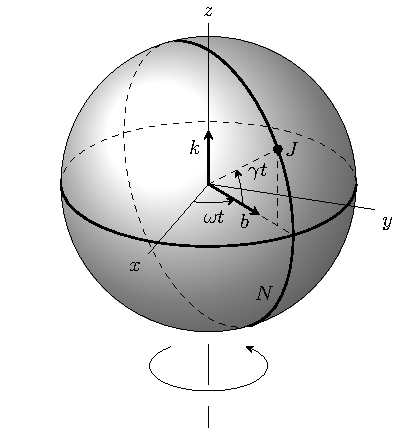
\includegraphics{sphereWithLines}
\caption{دو گردش کی خطی میل (مثال \حوالہ{مثال_الاحصاء_دو_گردش_کی_میل})}
\label{شکل_مثال_الاحصاء_دو_گردش_کی_میل}
\end{figure}
\انتہا{مثال}
%=================================

\حصہء{سوالات}
سوال \حوالہ{سوال_الاحصاء_تعین_گر_الف} تا سوال \حوالہ{سوال_الاحصاء_تعین_گر_ب} میں حرکت کرتی جسم کا تعین گر سمتیہ \عددی{\bM{r}(t)} ہے جہاں \عددی{t(>0)} وقت کو ظاہر کرتی ہے۔اس راہ کی شکل بیان کریں۔سمتیہ رفتار، رفتار اور اسراع دریافت کریں۔

%===================
\ابتدا{سوال}\شناخت{سوال_الاحصاء_تعین_گر_الف}\quad
$\bM{r}=t\bM{j}$\\
جوابات:
$\bM{v}=\bM{j},\quad \abs{\bM{v}}=1,\quad \bM{a}=0$
\انتہا{سوال}
%====================== 
\ابتدا{سوال}\quad
$\bM{r}=t^3\bM{j}$\\
جوابات:
$\bM{v}=3t^2\bM{j},\quad \abs{\bM{v}}=3t^2,\quad \bM{a}=6t\bM{j}$
\انتہا{سوال}
%====================== 
\ابتدا{سوال}\quad
$\bM{r}=(t^2-3t)\bM{j}$\\
جوابات:
$\bM{v}=(2t-3)\bM{j},\quad \abs{\bM{v}}=\abs{2t-3},\quad \bM{a}=2\bM{j}$
\انتہا{سوال}
%====================== 
\ابتدا{سوال}\quad
$\bM{r}=t^2\bM{i}-t\bM{j}$\\
جوابات:
$\bM{v}=2t\bM{i}-\bM{j},\quad \abs{\bM{v}}=\abs{\sqrt{4t^2+1}},\quad \bM{a}=2\bM{i}$
\انتہا{سوال}
%====================== 
\ابتدا{سوال}\quad
$\bM{r}=\cos t \,\bM{i}$\\
جوابات:
$\bM{v}=-\sin t\, \bM{j},\quad \abs{\bM{v}}=\abs{\sin t},\quad \bM{a}=-\cos t\,\bM{j}$
\انتہا{سوال}
%====================== 
\ابتدا{سوال}\quad
$\bM{r}=2\cos 5t \,\bM{i}-4\sin 3t \,\bM{j}$\\
جوابات:
$\bM{v}=-10\sin 5t\, \bM{i}-12\cos 3t\,\bM{j},\,\,\abs{\bM{v}}=\abs{\sqrt{100\sin^2 5t+144\cos^2 3t}}\\ \bM{a}=-50\cos 5t\,\bM{i}+36\sin 3t \,\bM{j}$
\انتہا{سوال}
%====================== 
\ابتدا{سوال}\quad
$\bM{r}=3\cos t^2 \,\bM{i}+2\sin t^2 \,\bM{j}$\\
جوابات:
$\bM{v}=-6t\sin t^2\, \bM{i}+4t\cos t^2\,\bM{j},\,\,\abs{\bM{v}}=\abs{\sqrt{36t^2\sin^2 t^2+16t^2\cos^2 t^2}}\\ 
\bM{a}=(-6\sin t^2-12t^2\cos t^2)\,\bM{i}+(4\cos t^2-8t^2\sin t^2) \,\bM{j}$
\انتہا{سوال}
%====================== 
\ابتدا{سوال}\شناخت{سوال_الاحصاء_تعین_گر_ب}\quad
$\bM{r}=5t^2 \,\bM{i}+3t \,\bM{j}+t^3\,\bM{k}$\\
جوابات:
$\bM{v}=10t\, \bM{i}+3\,\bM{j}+3t^2\,\bM{k},\,\,\abs{\bM{v}}=\abs{\sqrt{9t^4+100t^2+9}}\\ 
\bM{a}=10\,\bM{i}+6t \,\bM{k}$
\انتہا{سوال}
%====================== 
\ابتدا{سوال}زمین سے چاند تک کا فاصلہ \عددی{\SI{3.85e8}{\meter}} ہے اور زمین کے گرد چاند \عددی{27.322} دن یعنی \عددی{\SI{2.36e6}{\second}} میں ایک چکر پورا کرتا ہے۔زمین کے رخ چاند کی مرکز مائل اسراع دریافت کریں۔

جواب:\عددی{\abs{\bM{a}}=\SI{0.0027}{\meter\per\second\squared}} جو سطح زمین پر اسراع \عددی{g=\SI{9.8}{\meter\per\second\squared}} سے \عددی{3593} گنا کم ہے۔ 
\انتہا{سوال}
%=======================
\ابتدا{سوال}
وہ حرکت دریافت کریں جس کی اسراع مستقل قیمت ہو۔

جواب:
$\bM{r}(t)=\bM{a}_0\tfrac{t^2}{2}+\bM{v}_0t+\bM{x}_0$
جہاں \عددی{\bM{a}_0}، \عددی{\bM{v}_0} اور \عددی{\bM{x}_0} مستقل قیمتیں ہیں۔
\انتہا{سوال}
%=========================
\ابتدا{سوال}
\عددی{\bM{\omega}=\omega \bM{k}} اور \عددی{\bM{r}=R\cos \omega t\bM{i}+R\sin \omega t\bM{j}} لیتے ہوئے مساوات \حوالہ{مساوات_سمتیات_سمتی_رفتار_رداس_زاویائی_رفتار} کے تفرق  سے مساوات \حوالہ{مساوات_الاحصاء_اسراع_رفتار_حرکت} حاصل کریں۔
\انتہا{سوال}
%=======================
\ابتدا{سوال}
اگر ایک جسم کی حرکت \عددی{\bM{r}(t)} سے ظاہر کی جائے جہاں \عددی{t} وقت ہے تب \عددی{t=\phi{\tilde{t}}} تبادلے سے کیا مراد ہو گا؟

جواب:راہ تبدیل نہیں ہو گی البتہ راہ پر حرکت کی نوعیت تبدیل ہو گی۔
\انتہا{سوال}
%==========================

\حصہ{زنجیری ترکیب اور متعدد متغیرات کے تفاعل کا اوسط قیمت مسئلہ}
ہم متعدد متغیرات پر مبنی تفاعل کی خصوصیات پر غور کرتے ہیں۔ہم دو متغیرات کے تفاعل کو استعمال کرتے ہوئے  نتائج حاصل کریں گے جو زیادہ متغیرات کے تفاعل کے لئے بھی درست ہوں گے۔

نقطہ \عددی{(x_0,y_0)} پر تفاعل \عددی{f(x,y)}  اس صورت \اصطلاح{استمراری}\فرہنگ{استمراری}\حاشیہب{continuous}\فرہنگ{continuous} ہو گا جب اس نقطے کے \اصطلاح{ہمسائیگی}\حاشیہد{ہمسائیگی سے مراد \عددی{xy} سطح میں قرص \عددی{(x-x_0)^2+(y-y_0)^2<r^2} ہے جہاں \عددی{r>0} ہے۔} میں \عددی{f} معین ہو اور کسی بھی مثبت عدد \عددی{\epsilon} (جو غیر صفر اور کتنا ہی چھوٹا کیوں نا ہو) کے لئے ہم ایسا مثبت عدد \عددی{\sigma} تلاش کر سکتے ہیں کہ اس کے نقطے کے ہمسائیگی  قرص 
\begin{align}
(x-x_0)^2+(y-y_0)^2<\sigma^2
\end{align}
میں تمام \عددی{(x,y)} پر درج ذیل ہو۔
\begin{align}
\abs{f(x,y)-f(x_0,y_0)}<\epsilon
\end{align}

جیومیٹریائی طور پر \عددی{(x_0,y_0)} پر \عددی{f(x,y)} کے استمراری ہونے سے مراد یہ ہے کہ \عددی{f(x_0,y_0)} کو قطع \عددی{2\epsilon} کا وسط لیتے ہوئے  ہم غیر صفر رداس \عددی{\sigma} کا ایسا قرص تلاش کر سکتے ہیں جس کا مرکز \عددی{(x_0,y_0)} ہو اور اس قرص  پر تمام \عددی{(x,y)} کا مطابقتی \عددی{f(x,y)} اس قطع پر پایا جاتا ہو (شکل \حوالہ{شکل_الاحصاء_استمرار_تعریف})۔
\begin{figure}
\centering
\begin{subfigure}{0.5\textwidth}
\centering
\begin{tikzpicture}
\draw(0,0)--++(2.5,0)node[below]{$x$};
\draw(0,0)--++(0,2.5)node[left]{$y$};
\draw(1.25,1.25)circle (1);
\draw[-stealth] (1.25,1.25)node[ocirc]{}node[below]{$(x_0,y_0)$} --++(30:1)node[pos=0.5,above]{$\sigma$};
\end{tikzpicture}
\end{subfigure}%
\begin{subfigure}{0.5\textwidth}
\centering
\begin{tikzpicture}
\draw(-1.5,0)--(1.5,0);
\draw(0,0)node[below]{$f(x_0,y_0)$}--++(0,0.15)++(0,0.15)--++(0,0.15);
\draw(-1.25,0)--++(0,0.15)++(0,0.15)--++(0,0.15);
\draw(1.25,0)--++(0,0.15)++(0,0.15)--++(0,0.15);
\draw[stealth-stealth](-1.25,0.15+0.15+0.15/2)--++(1.25,0)node[pos=0.5,fill=white]{$\epsilon$};
\draw[stealth-stealth](0,0.15+0.15+0.15/2)--++(1.25,0)node[pos=0.5,fill=white]{$\epsilon$};
\end{tikzpicture}
\end{subfigure}%
\caption{دو متغیرات کے تفاعل کی استمرار}
\label{شکل_الاحصاء_استمرار_تعریف}
\end{figure}

ہم ابتدائی علم الاحصاء سے جانتے ہیں کہ اگر \عددی{w} متغیر \عددی{x} کا قابل تفرق تفاعل ہو اور \عددی{x} از خود \عددی{t} کا قابل تفرق تفاعل ہو تب درج ذیل لکھا جا سکتا ہے جس کو تفرق کا زنجیری قاعدہ کہتے ہیں۔
\begin{align}
\frac{\dif w}{\dif t}=\frac{\dif w}{\dif x}\frac{\dif x}{\dif t}
\end{align} 
درج ذیل مسئلہ  تفرق کی زنجیری قاعدے کو عمومی بناتا ہے۔

%================
\ابتدا{مسئلہ}\شناخت{مسئلہ_الاحصاء_زنجیری_قاعدہ}\quad (زنجیری قاعدہ)\\
فرض کریں کہ \عددی{xy} سطح میں \اصطلاح{دائرہ کار}\فرہنگ{دائرہ کار}\حاشیہب{domain}\فرہنگ{domain} \عددی{D}\حاشیہد{دائرہ کار \عددی{D} \ترچھا{جڑی} ہوئے نقطوں کا \ترچھا{کھلا} سلسلہ ہے، جہاں \اصطلاح{جڑا} ہونے سے مراد یہ ہے کہ \عددی{D} کے کسی بھی دو نقطوں کو متناہی تعداد کے ایسے سیدھے قطعات سے ملایا جا سکتا ہے جن کے تمام نقطے \عددی{D} کا حصہ ہوں، اور \اصطلاح{کھلا} سے مراد یہ ہے کہ \عددی{D} میں ہر نقطے کی ہمسائیگی  کے تمام نقطے بھی \عددی{D} کا حصہ ہیں۔مثلاً کسی مستطیل یا دائرے کا اندرونی حصہ دائرہ کار ہو گا۔} میں تفاعل \عددی{w=f(x,y)} استمراری ہے  اور  اس تفاعل کے درجہ ایک جزوی تفرقات بھی \عددی{D} میں استمراری ہیں۔مزید فرض کریں کہ کسی وقفہ \عددی{T} میں \عددی{x=x(t)} اور \عددی{y=y(t)} قابل تفرق تفاعل ہیں جہاں \عددی{T} میں ہر \عددی{t} کا مطابقتی  نقطہ \عددی{[x(t),y(t)]}، دائرہ کار \عددی{D} میں پایا جاتا ہے۔ایسی صورت میں \عددی{T} میں تمام \عددی{t} کے لئے  \عددی{w=f[x(t),y(t)]} قابل تفرق ہو گا یعنی:
\begin{align}\label{مساوات_الاحصاء_زنجیری_تفرق_قاعدہ_الف}
\frac{\dif w}{\dif t}=\frac{\partial w}{\partial x}\frac{\dif x}{\dif t}+\frac{\partial w}{\partial y}\frac{\dif y}{\dif t}
\end{align}   
\انتہا{مسئلہ}
%======================
\ابتدا{ثبوت}
ہم \عددی{T} میں \عددی{t}  پر \عددی{\Delta t} اتنا چھوٹا چنتے ہیں کہ \عددی{t+\Delta t} بھی \عددی{T} کا حصہ ہو۔مزید ہم 
\begin{align}\label{مساوات_الاحصاء_زنجیری_الف}
\Delta x=x(t+\Delta t)-x(t),\quad \Delta y=y(t+\Delta t)-y(t)
\end{align} 
اور
\begin{align}\label{مساوات_الاحصاء_زنجیری_ب}
\Delta w=f(x+\Delta x,y+\Delta y)-f(x,y)
\end{align}
لیتے ہیں۔مساوات \حوالہ{مساوات_الاحصاء_زنجیری_ب} میں \عددی{f(x,y+\Delta y)} جمع اور منفی کرتے ہوئے درج ذیل لکھا جا سکتا ہے۔
\begin{align*}
\Delta w=[f(x+\Delta x,y+\Delta y)-f(x,y+\Delta y)]+[f(x,y+\Delta y)-f(x,y)]
\end{align*}
درج بالا مساوات کے قوسین پر باری باری ایک متغیر کے تفاعل کا اوسط قیمت مسئلہ لاگو کرتے ہوئے
\begin{align}\label{مساوات_الاحصاء_زنجیری_پ}
\Delta w=\Delta x \left.\frac{\partial f}{\partial x} \right|_{x_1,y+\Delta y}+\Delta y \left.\frac{\partial f}{\partial y} \right|_{x,y_1}
\end{align}  
حاصل ہوتا ہے جہاں \عددی{x} اور \عددی{x+\Delta x} کے درمیان کہیں \عددی{x_1} پایا جاتا ہے، \عددی{y} اور \عددی{y+\Delta y} کے درمیان کہیں \عددی{y_1} پایا جاتا ہے۔مساوات \حوالہ{مساوات_الاحصاء_زنجیری_پ} کے دونوں اطراف کو \عددی{\Delta t} سے تقسیم کرتے اور \عددی{\Delta t \to 0} لیتے ہوئے، اور چونکہ
 \عددی{\tfrac{\partial f}{\partial x}} اور \عددی{\tfrac{\partial f}{\partial y}} کو استمراری تصور کیا گیا ہے، مساوات  \حوالہ{مساوات_الاحصاء_زنجیری_الف} حاصل ہوتا ہے۔
\انتہا{ثبوت}
%========================

درج بالا مسئلے کو وسعت دیتے ہوئے درج ذیل مسئلہ اخذ کیا جا سکتا ہے۔

%==========
\ابتدا{مسئلہ}\شناخت{مسئلہ_الاحصاء_جزوی_تفرقات}
فرض کریں کہ \عددی{xy} سطح میں \اصطلاح{دائرہ کار} \عددی{D} پر تفاعل \عددی{w=f(x,y)} استمراری ہے  اور  اس تفاعل کے درجہ ایک جزوی تفرقات بھی \عددی{D} میں استمراری ہیں۔مزید فرض کریں کہ \عددی{uv} سطح میں کسی وقفہ \عددی{B} میں \عددی{x=x(u,v)} اور \عددی{y=y(u,v)} قابل جزوی تفرق تفاعل ہیں جہاں \عددی{B} میں ہر \عددی{(u,v)} کا مطابقتی نقطہ \عددی{[x(u,v),y(u,v)]}، دائرہ کار \عددی{D} میں پایا جاتا ہے۔ایسی صورت میں \عددی{B} میں تفاعل  \عددی{w=f[x(u,v),y(u,v)]} معین ہو گا اور \عددی{B} میں تمام \عددی{u} اور \عددی{v} کے لئے اس تفاعل کے جزوی تفرقات  درج ذیل ہوں گے۔
\begin{gather}
\begin{aligned}
\frac{\partial w}{\partial u}&=\frac{\partial w}{\partial x}\frac{\partial x}{\partial u}+\frac{\partial w}{\partial y}\frac{\partial y}{\partial u}\\
\frac{\partial w}{\partial v}&=\frac{\partial w}{\partial x}\frac{\partial x}{\partial v}+\frac{\partial w}{\partial y}\frac{\partial y}{\partial v}
\end{aligned}
\end{gather}
\انتہا{مسئلہ}
%====================

\عددی{u} یا \عددی{v} کو غیر متغیر رکھتے ہوئے مسئلہ \حوالہ{مسئلہ_الاحصاء_زنجیری_قاعدہ} کے اطلاق سے  درج بالا مسئلہ ثابت ہوتا ہے۔

ابتدائی علم الاحصاء  سے ہم جانتے ہیں کہ قابل تفرق تفاعل \عددی{f(x)} کے لئے درج ذیل لکھا جا سکتا ہے جہاں \عددی{x_0} اور \عددی{x_0+h} کے درمیان موزوں نقطے پر تفرق لیا جاتا ہے۔
\begin{align*}
f(x_0+h)-f(x_0)=h\frac{\dif f}{\dif x}
\end{align*}
اس کو احصاء تفرقیات کا مسئلہ اوسط قیمت کہتے ہیں جس کو  وسعت دے کر  دو متغیرات کے تفاعل پر لاگو  کیا جا سکتا ہے۔

%==================
\ابتدا{مسئلہ}\شناخت{مسئلہ_الاحصاء_اوسط_قیمت}\quad (مسئلہ اوسط قیمت)\\
فرض کریں کہ دائرہ کار \عددی{D} میں تفاعل \عددی{f(x,y)} استمراری ہے اور اس تفاعل کے درجہ ایک جزوی تفرقات بھی \عددی{D} میں استمراری ہیں۔ مزید فرض کریں کہ \عددی{(x_0,y_0)} اور  \عددی{(x_0+h,y_0+k)} دائرہ کار \عددی{D} میں پائے جانے والے ایسے نقطے ہیں کہ انہیں جوڑنے والا سیدھا قطع  بھی \عددی{D} میں پائی جاتی ہو (شکل \حوالہ{شکل_مسئلہ_الاحصاء_اوسط_قیمت})۔ایسی صورت میں 
\begin{align}\label{مساوات_الاحصاء_مسئلہ_زنجیری_الف}
f(x_0+h,y_0+k)-f(x_0,y_0)=h\frac{\partial f}{\partial x}+k\frac{\partial f}{\partial y}
\end{align}
لکھا جا سکتا ہے جہاں جزوی تفرقات کو  اس قطع پر موزوں نقطے پر حاصل کیا جاتا ہے۔
\begin{figure}
\centering
\begin{tikzpicture}
\draw[smooth cycle] plot coordinates {(0,0)(-2,0.75)(-1,1.75)(0,2)(1.5,2)(3.2,1.75)(2,0.25)};
\draw(0,0.7)node[ocirc]{}node[below]{$(x_0,y_0)$}--(1.5,1)node[ocirc]{}node[above]{$(x_0+h,y_0+k)$};
\draw(0,1.75)node{$D$};
\end{tikzpicture}
\caption{مسئلہ اوسط قیمت}
\label{شکل_مسئلہ_الاحصاء_اوسط_قیمت}
\end{figure}
\انتہا{مسئلہ}
%======================
\ابتدا{ثبوت}
درج ذیل
\begin{align*}
x&=x_0+th,\quad y=y_0+tk\quad (0\le t \le 1)\\
F(t)&=f(x_0+th,y_0+tk)
\end{align*}
سے
\begin{align*}
f(x_0+h,y_0+k)=F(1),\quad f(x_0,y_0)=F(0)
\end{align*}
لکھا جا سکتا ہے۔ایک متغیر تفاعل کے  مسئلہ اوسط قیمت کے تحت \عددی{0} اور \عددی{1} کے درمیان  ایسی قیمت \عددی{t_1}  پائی جاتی ہے جس کے لئے  درج ذیل لکھا جا سکتا ہے۔ 
\begin{align}\label{مساوات_الاحصاء_مسئلہ_زنجیری_ب}
f(x_0+h,y_0+k)-f(x_0,y_0)=F(1)-F(0)=F'(t_1)
\end{align}
اب چونکہ \عددی{\tfrac{\dif x}{\dif t}=h} اور \عددی{\tfrac{\dif y}{\dif t}=k} ہیں لہٰذا مسئلہ \حوالہ{مسئلہ_الاحصاء_زنجیری_قاعدہ} کے تحت
\begin{align}\label{مساوات_الاحصاء_مسئلہ_زنجیری_پ}
F'=\frac{\partial f}{\partial x}h+\frac{\partial f}{\partial y}k
\end{align}
ہو گا جہاں دائیں ہاتھ تفرقات کو نقطہ \عددی{(x_0+t_1h,y_0+t_1k)} پر حاصل کیا جائے گا جو اس قطع پر واقع ہے جس کے سر \عددی{(x_0,y_0)} اور \عددی{(x_0+h,y_0+k)} ہیں۔مساوات \حوالہ{مساوات_الاحصاء_مسئلہ_زنجیری_پ} کو مساوات \حوالہ{مساوات_الاحصاء_مسئلہ_زنجیری_ب} میں پر کرنے سے  مساوات \حوالہ{مساوات_الاحصاء_مسئلہ_زنجیری_الف} حاصل ہوتا ہے۔
\انتہا{ثبوت}
%========================

تین متغیرات کے تفاعل \عددی{f(x,y,z)} جو مسئلہ \حوالہ{مسئلہ_الاحصاء_اوسط_قیمت} میں دیے گئے شرائط کے مماثل شرائط پر پورا اترتا ہو کے لئے بالکل اسی مسئلے کی طرح درج ذیل لکھا جا سکتا ہے
\begin{align}\label{مساوات_الاحصاء_مسئلہ_زنجیری_ت}
f(x_0+h,y_0+k,z_0+l)-f(x_0,y_0,z_0)=h\frac{\partial f}{\partial x}+k\frac{\partial f}{\partial y}+l\frac{\partial f}{\partial z}
\end{align}
جہاں جزوی تفرقات کو \عددی{(x_0,y_0,z_0)} تا \عددی{(x_0+h,y_0+k,z_0+l)} قطع پر موزوں نقطے پر حاصل کیا جائے گا۔

%===================
\حصہء{سوالات}
سوال \حوالہ{سوال_الاحصاء_زنجیری_قاعدہ_الف} تا سوال \حوالہ{سوال_الاحصاء_زنجیری_قاعدہ_ب} میں مساوات \حوالہ{مساوات_الاحصاء_زنجیری_تفرق_قاعدہ_الف} کی مدد سے \عددی{\tfrac{\dif w}{\dif t}} دریافت کریں۔

%===============
\ابتدا{سوال}\شناخت{سوال_الاحصاء_زنجیری_قاعدہ_الف}\quad
$w=x-y,\quad x=t,\quad y=\ln t$\\
جواب:
$1-\tfrac{1}{t}$
\انتہا{سوال}
%========================
\ابتدا{سوال}\quad
$w=\sqrt{x^2+y^2},\quad x=e^{-t},\quad y=e^{t}$\\
جواب:
$\tfrac{e^{2t}-e^{-2t}}{\sqrt{e^{2t}+e^{-2t}}}$
\انتہا{سوال}
%========================
\ابتدا{سوال}\quad
$w=\tfrac{x}{y},\quad x=g(t),\quad y=h{t}$\\
جواب:
$\tfrac{g'h-gh'}{h^2}$
\انتہا{سوال}
%========================
\ابتدا{سوال}\شناخت{سوال_الاحصاء_زنجیری_قاعدہ_ب}\quad
$w=\tfrac{x}{y},\quad x=\cos t,\quad y=\sin t$\\
جواب:
$-\cosec^{\,2} t$
\انتہا{سوال}
%========================
\ابتدا{سوال}
فرض کریں کہ \عددی{w=f(x,y,z)} ہے جہاں \عددی{x}، \عددی{y} اور \عددی{z} از خود \عددی{t} کے تفاعل ہیں۔ثابت کریں کہ مسئلہ \حوالہ{مسئلہ_الاحصاء_زنجیری_قاعدہ} کی طرز کے شرائط کی صورت میں درج ذیل ہو گا۔
\begin{align}\label{مساوات_الاحصاء_زنجیری_تین_متغیرات}
\frac{\dif w}{\dif t}=\frac{\partial w}{\partial x}\frac{\dif x}{\dif t}+\frac{\partial w}{\partial y}\frac{\dif y}{\dif t}+\frac{\partial w}{\partial z}\frac{\dif z}{\dif t}
\end{align}
\انتہا{سوال}
%===================
سوال \حوالہ{سوال_الاحصاء_زنجیری_تین_متغیرات_الف} اور سوال \حوالہ{سوال_الاحصاء_زنجیری_تین_متغیرات_ب} میں مساوات \حوالہ{مساوات_الاحصاء_زنجیری_تین_متغیرات} کی مدد سے \عددی{\tfrac{\dif w}{\dif t}} دریافت کریں۔

%==========================
\ابتدا{سوال}\شناخت{سوال_الاحصاء_زنجیری_تین_متغیرات_الف}\quad
$w=x^2+y^2+z^2,\quad x=t^2,\quad y=\ln t,\quad z=e^t$\\
جواب:
$\tfrac{2}{t}\ln t+2e^{2t}+4t^3$
\انتہا{سوال}
%=========================
\ابتدا{سوال}\شناخت{سوال_الاحصاء_زنجیری_تین_متغیرات_ب}\quad
$w=\sqrt{x^2+y^2+z^2},\quad x=\cos t,\quad y=\sin t,\quad z=t$\\
جواب:
$\tfrac{t}{\sqrt{1+t^2}}$
\انتہا{سوال}
%=========================
\ابتدا{سوال}
مسئلہ \حوالہ{مسئلہ_الاحصاء_جزوی_تفرقات} کو ثابت کریں۔
\انتہا{سوال}
%=======================
سوال \حوالہ{سوال_الاحصاء_جزوی_تفرقات_الف} تا سوال \حوالہ{سوال_الاحصاء_جزوی_تفرقات_ب} میں \عددی{\tfrac{\partial w}{\partial u}} اور \عددی{\tfrac{\partial w}{\partial v}} دریافت کریں۔

%===================
\ابتدا{سوال}\شناخت{سوال_الاحصاء_جزوی_تفرقات_الف}\quad
$w=\ln(x^2+y^2),\quad x=e^u\cos v,\quad y=e^u\sin v$\\
جواب:
$2,\,\, 0$
\انتہا{سوال}
%======================
\ابتدا{سوال}\quad
$w=xy,\quad x=e^u\cos v,\quad y=e^u\sin v$\\
جواب:
$e^{2u}\sin 2v,\,\,e^{2u}\cos 2v$
\انتہا{سوال}
%======================
\ابتدا{سوال}\شناخت{سوال_الاحصاء_جزوی_تفرقات_ب}\quad
$w=x^2-y^2,\quad x=u^2-v^2,\quad y=2uv$\\
جواب:
$4u(u^2-3v^2),\,\,4v(v^2-3u^2)$
\انتہا{سوال}
%======================
\ابتدا{سوال}
مساوات \حوالہ{مساوات_الاحصاء_مسئلہ_زنجیری_ت} حاصل کریں۔
\انتہا{سوال}
%======================
\ابتدا{سوال}
فرض کریں کہ \عددی{w=f(x,y)} ہے جہاں \عددی{x=r\cos \theta} اور \عددی{y=r\sin \theta} ہیں۔درج ذیل ثابت کریں۔
\begin{align*}
\left(\frac{\partial w}{\partial r}\right)^2+\frac{1}{r^2}\left(\frac{\partial w}{\partial \theta}\right)^2=\left(\frac{\partial w}{\partial x}\right)^2+\left(\frac{\partial w}{\partial y}\right)^2
\end{align*}
جواب:درج ذیل استعمال کرتے ہوئے با آسانی ثابت ہو گا۔
\begin{align*}
\frac{\partial w}{\partial r}&=\frac{\partial w}{\partial x}\frac{\partial x}{\partial r}+\frac{\partial w}{\partial y}\frac{\partial y}{\partial r}=
\frac{\partial w}{\partial x}\cos \theta +\frac{\partial w}{\partial y}\sin \theta \\
\frac{\partial w}{\partial \theta}&=\frac{\partial w}{\partial x}\frac{\partial x}{\partial \theta}+\frac{\partial w}{\partial y}\frac{\partial y}{\partial \theta}=
-\frac{\partial w}{\partial x}r\sin \theta +\frac{\partial w}{\partial y}r\cos\theta 
\end{align*}
\انتہا{سوال}
%======================
\ابتدا{سوال}
فرض کریں کہ \عددی{w=f(v,z)}ہے جہاں  \عددی{v=x+ct} اور  \عددی{z=x-ct} ہیں جبکہ  \عددی{c} مستقل قیمت  ہے۔درج ذیل ثابت کریں جہاں تمام تفرقات کو ممکن تصور کریں۔ \عددی{w_{xx}} سے مراد \عددی{\tfrac{\partial ^2 w}{\partial x^2}} ہے۔
\begin{align*}
c^2w_{xx}-w_{tt}=4c^2w_{vz}
\end{align*} 
\انتہا{سوال}
%=========================
\ابتدا{سوال}
فرض کریں کہ \عددی{w=f(x,y)} ہے جہاں \عددی{x=r\cos \theta} اور \عددی{y=r\sin \theta} ہیں۔درج ذیل ثابت کریں۔
\begin{align*}
w_{xx}+w_{yy}=w_{rr}+\frac{1}{r}w_r+\frac{1}{r^2}w_{\theta \theta}
\end{align*}
جواب:
$r=\sqrt{x^2+y^2}$
اور
$\theta=\tan^{-1}\frac{y}{x}$
سے درج ذیل حاصل کرتے ہوئے ثابت ہو گا۔
\begin{align*}
r_x&=\frac{x}{r},\,\, \theta_x=-\frac{y}{r^2},\,\, r_{xx}=\frac{y^2}{r^3},\quad \text{وغیرہ}\\
 w_{xx}&=x^2r^{-2}w_{rr}-2xyr^{-3}w_{r\theta}+y^2r^{-4}w_{\theta\theta}+y^2r^{-3}w_r+2xyr^{-4}w_{\theta},\quad \text{وغیرہ}
\end{align*}
\انتہا{سوال}
%=======================

\حصہ{سمتی تفرق، غیر سمتی میدان کی ڈھلوان}
ہم فضا میں غیر سمتی میدان \عددی{f(P)=f(x,y,z)}  پر غور کرتے ہیں (حصہ \حوالہ{حصہ_الاحصاء_غیر_سمتی-_اور_سمتی_میدان})۔ہم جانتے ہیں کہ  \عددی{x}، \عددی{y} اور \عددی{z}  رخ  میں تفاعل کی تبدیلی کی شرح بالترتیب \عددی{\tfrac{\partial f}{\partial x}}، \عددی{\tfrac{\partial f}{\partial y}} اور \عددی{\tfrac{\partial f}{\partial z}} ہے۔ آئیں کسی بھی رخ اس تفاعل کی تبدیلی کی شرح یعنی \اصطلاح{سمتی تفرق} حاصل کریں۔

ہم فضا میں کوئی نقطہ \عددی{P} اور اس نقطے پر کوئی رخ چنتے ہیں۔اس رخ  کو اکائی سمتیہ \عددی{\bM{b}} سے ظاہر کرتے ہیں۔نقطہ \عددی{P} سے \عددی{s} فاصلے پر  \عددی{\bM{b}} کی رخ سیدھے خط \عددی{C} پر نقطہ \عددی{Q} پایا جاتا ہے (شکل \حوالہ{شکل_الاحصاء_سمتی_تفرق})۔اگر درج ذیل حد
\begin{align}\label{مساوات_الاحصاء_سمتی_تفرق_الف}
\frac{\partial f}{\partial s}=\lim_{s\to 0}\frac{f(Q)-f(P)}{s}
\end{align}
موجود ہو تب اس کو \عددی{P} پر \عددی{\bM{b}} کی رخ \عددی{f} کی \اصطلاح{سمتی تفرق}\فرہنگ{سمتی!تفرق}\فرہنگ{تفرق!سمتی}\حاشیہب{directional derivative}\فرہنگ{directional derivative}\فرہنگ{derivative!directional} کہتے ہیں۔ظاہر ہے کہ \عددی{\tfrac{\partial f}{\partial s}} در حقیقت \عددی{P} پر \عددی{\bM{b}} کی رخ  \عددی{f} کی شرح تبدیلی ہے۔ 
\begin{figure}
\centering
\begin{tikzpicture}
\pgfmathsetmacro{\ang}{20}
\draw(0,0)--++(\ang:3.5)node[below]{$C$};
\draw(0,0)node[below]{$P$}--++(\ang:2)node[ocirc]{}node[below]{$Q$};
\draw[-latex](0,0)node[ocirc]{}--++(\ang:1)node[below]{$\bM{b}$};
\draw [decorate,decoration={brace,amplitude=5pt},shift={(\ang+90:5pt)}](0,0) --++(\ang:1)node [black,midway,shift={(\ang+90:9pt)}] {\footnotesize$s$};
\end{tikzpicture}
\caption{سمتی تفرق}
\label{شکل_الاحصاء_سمتی_تفرق}
\end{figure}

یوں \عددی{P} پر \عددی{f} کے لامتناہی تعداد میں سمتی تفرقات پائے جاتے ہیں۔اگر \عددی{P} کا تعین گر سمتیہ \عددی{\bM{a}} ہو تب \عددی{C}  کو درج ذیل لکھا جا سکتا ہے 
\begin{align}\label{مساوات_الاحصاء_سمتی_تفرق_ب}
\bM{r}(s)=x(x)\bM{i}+y(s)\bM{j}+z(s)\bM{k}=\bM{a}+s\bM{b}\quad \quad (s\ge 0)
\end{align}
اور \عددی{\tfrac{\partial f}{\partial s}} سے مراد \عددی{C} پر \عددی{f[x(s),y(s),z(s)]} کا لمبائی \عددی{s} کے ساتھ تفرق ہے۔اب اگر \عددی{f} کے استمراری جزوی تفرقات پائے جاتے ہوں تب زنجیری قاعدے (مسئلہ \حوالہ{مسئلہ_الاحصاء_زنجیری_قاعدہ}) کے تحت درج ذیل لکھا جا سکتا ہے
\begin{align}\label{مساوات_الاحصاء_سمتی_تفرق_پ}
\frac{\partial f}{\partial s}=\frac{\partial f}{\partial x}x'+\frac{\partial f}{\partial y}y'+\frac{\partial f}{\partial z}z'
\end{align}
جہاں \عددی{x'=\tfrac{\dif x}{\dif s}}  کو \عددی{s=0} پر حاصل کیا جاتا ہے۔اب مساوات \حوالہ{مساوات_الاحصاء_سمتی_تفرق_ب} سے
\begin{align*}
\bM{r}'=x'\bM{i}+y'\bM{j}+z'\bM{k}=\bM{b}
\end{align*}
لکھا جا سکتا ہے جس کو دیکھ کر  خیال آتا ہے کہ  سمتیہ
\begin{align}\label{مساوات_الاحصاء_سمتی_تفرق_ت}
f_{\text{ڈھلوان}}=\frac{\partial f}{\partial x}\bM{i}+\frac{\partial f}{\partial y}\bM{j}+\frac{\partial f}{\partial z}\bM{k}
\end{align}
متعارف کرنے سے مساوات \حوالہ{مساوات_الاحصاء_سمتی_تفرق_پ} کو اندرونی ضرب (ضرب نقطہ) کی صورت میں لکھا جا سکتا ہے۔
\begin{align}\label{مساوات_الاحصاء_سمتی_تفرق_ٹ}
\frac{\partial f}{\partial s}=\bM{b}\cdot f_{\text{ڈھلوان}} \quad \quad (\abs{\bM{b}}=1)
\end{align}
سمتیہ 
$f_{\text{ڈھلون}}$
کو غیر سمتی تفاعل \عددی{f} کی \اصطلاح{ڈھلوان}\فرہنگ{ڈھلوان}\حاشیہب{gradient}\فرہنگ{gradient} کہتے ہیں۔

تفرقی عامل \عددی{\nabla}\حاشیہد{\عددی{\nabla} یونانی حرف تہجی ہے جو نیبلا کہلاتا ہے۔}
\begin{align*}
\nabla =\frac{\partial}{\partial x}\bM{i}+\frac{\partial}{\partial y}\bM{j}+\frac{\partial}{\partial z}\bM{k}
\end{align*}
متعارف کرتے ہوئے  مساوات \حوالہ{مساوات_الاحصاء_سمتی_تفرق_ت} کو 
\begin{align}\label{مساوات_الاحصاء_سمتی_تفرق_ث}
f_{\text{ڈھلوان}}=\nabla f=\frac{\partial f}{\partial x}\bM{i}+\frac{\partial f}{\partial y}\bM{j}+\frac{\partial f}{\partial z}\bM{k}
\end{align}
اور مساوات \حوالہ{مساوات_الاحصاء_سمتی_تفرق_ٹ} کو 
\begin{align}\label{مساوات_الاحصاء_سمتی_تفرق_ج}
\frac{\partial f}{\partial s}=\bM{b}\cdot \nabla f\quad \quad (\abs{\bM{b}}=1)
\end{align}
لکھا جا سکتا ہے۔

اگر \عددی{\bM{b}} کارتیسی \عددی{x} محور کی رخ ہو تب \عددی{\bM{b}=\bM{i}} ہو گا اور \عددی{f} کا سمتی تفرق درج ذیل ہو گا۔
\begin{align*}
\frac{\partial f}{\partial s}=\bM{b}\cdot \nabla f=\frac{\partial f}{\partial x}\bM{i}\cdot \bM{i}=\frac{\partial f}{\partial x}
\end{align*}
اسی طرح مثبت \عددی{y} اور مثبت \عددی{z} محور کی رخ سمتی تفرق بالترتیب \عددی{\tfrac{\partial f}{\partial y}} اور \عددی{\tfrac{\partial f}{\partial z}} ہوں گے۔

%==================
\ابتدا{مثال}\quad سمتی تفرق\\
غیر سمتی تفاعل \عددی{f(x,y,z)=x^2+2y-z^3} کا نقطہ \عددی{P:(-2,1,3)} پر \عددی{\bM{a}=3\bM{i}-4\bM{j}} کی رخ سمتی تفرق دریافت کریں۔

حل:چونکہ \عددی{\abs{\bM{a}}=5} ہے لہٰذا \عددی{\bM{a}} کی رخ اکائی سمتیہ
 \عددی{\bM{b}=\tfrac{\bM{a}}{\abs{\bM{a}}}=\tfrac{3}{5}\bM{i}-\tfrac{4}{5}\bM{j}} ہو گا۔ \عددی{f} کی ڈھلوان درج ذیل ہے۔
\begin{align*}
\nabla f=2x\bM{i}+2\bM{j}-3z^2\bM{k}\implies  \nabla f(P)=-4\bM{i}+2\bM{j}-27\bM{k}
\end{align*}
یوں نقطہ \عددی{P} پر \عددی{\bM{a}} کی رخ سمتی تفرق درج ذیل ملتا ہے۔
\begin{align*}
\frac{\partial f}{\partial s}=\bM{b}\cdot \nabla f=\frac{1}{5}(3\bM{i}-4\bM{j})\cdot (-4\bM{i}+2\bM{j}-27\bM{k})=-4
\end{align*}
حاصل جواب منفی ہے جس کا مطلب ہے کہ \عددی{\bM{a}} کی رخ  \عددی{f} گھٹتا ہے۔
\انتہا{مثال}
%========================

ہم اب ثابت کرتے ہیں کہ \عددی{\nabla f} کی قیمت اور رخ پر چنے گئے کارتیسی نظام کا کوئی اثر نہیں پایا جاتا ہے۔ 

مساوات \حوالہ{مساوات_الاحصاء_سمتی_تفرق_ت} سمتی تفرق دیتا ہے جو کسی دوسرے کارتیسی نظام میں درج ذیل لکھا جائے گا
\begin{align*}
f_{\text{ڈھلوان}}=\frac{\partial f}{\partial x^*}\bM{i}^*+\frac{\partial f}{\partial y^*}\bM{j}^*+\frac{\partial f}{\partial z^*}\bM{k}^*
\end{align*}
 جہاں \عددی{x^*}، \عددی{y^*} اور \عددی{z^*} دوسرے نظام کے محور جبکہ \عددی{\bM{i}^*}، \عددی{\bM{j}^*} اور \عددی{\bM{k}^*} اس کے مطابقتی اکائی سمتیات ہیں۔ان مساوات میں جزوی تفرقات پائے جاتے ہیں اور یہ کہنا مشکل ہو گا کہ دونوں مساوات سے یکساں ڈھلوان حاصل ہو گا۔ 

اب غیر سمتی تفاعل کی تعریف کے تحت نقطہ \عددی{P} پر \عددی{f} کی قیمت کا دارومدار \عددی{P} پر ہے نا کہ چنے گئے کارتیسی نظام پر۔اسی طرح \عددی{C} پر لمبائی \عددی{s} پر بھی چنے گئے کارتیسی نظام کا کوئی اثر نہیں پایا جاتا ہے۔یوں \عددی{\tfrac{\partial f}{\partial s}} پر چنے گئے کارتیسی نظام کا کوئی اثر نہیں ہو گا۔ اب مساوات \حوالہ{مساوات_الاحصاء_سمتی_تفرق_ج} کو درج ذیل لکھا جا سکتا ہے
\begin{align*}
\frac{\partial f}{\partial s}=\abs{\bM{b}}\abs{\nabla f}\cos \gamma=\abs{\nabla f}\cos \gamma
\end{align*}
جہاں \عددی{\bM{b}} اور \عددی{\nabla f} کے مابین زاویہ \عددی{\gamma} ہے۔ہم دیکھتے ہیں کہ  \عددی{\cos \gamma=1} یعنی \عددی{\gamma=0} پر \عددی{\tfrac{\partial f}{\partial s}} کی زیادہ سے زیادہ قیمت \عددی{\tfrac{\partial f}{\partial s}=\abs{\nabla f}} پائی جاتی ہے۔اب چونکہ \عددی{\tfrac{\partial f}{\partial s}} غیر متغیر ہے لہٰذا \عددی{\nabla f}  کی قیمت اور سمت پر کارتیسی نظام کا کوئی اثر نہیں ہو گا۔اس سے درج ذیل نتیجہ ملتا ہے۔

%===============
\ابتدا{مسئلہ}\quad ڈھلوان\\
ایسا غیر سمتی تفاعل \عددی{f(P)=f(x,y,z)}  جس کے استمراری ایک درجی جزوی تفرقات پائے جاتے ہوں کی ڈھلوان موجود ہے جس کی لمبائی اور رخ پر چنے گئے کارتیسی نظام محدد کا کوئی اثر نہیں پایا جاتا ہے۔اگر نقطہ \عددی{P} پر \عددی{f} کی ڈھلوان غیر صفر سمتیہ ہو تب \عددی{P} پر \عددی{f} کی زیادہ سے زیادہ تبدیلی ڈھلوان کی رخ ہو گی۔ 
\انتہا{مسئلہ}
%========================

ڈھلوان کی دوسری جیومیٹریائی خصلت جانتے ہیں۔فضا میں قابل تفرق غیر سمتی تفاعل \عددی{f(x,y,z)} پر غور کرتے ہیں۔ہر مستقل \عددی{c} کے لئے مساوات
\begin{align}\label{مساوات_الاحصاء_سمتی_تفرق_چ}
f(x,y,z)=c=\text{مستقل}
\end{align}
 سطح \عددی{S} کو ظاہر کرتا ہے۔\عددی{c} کے تمام قیمتیں لیتے ہوئے ہمیں نسل سطح ملتا ہے جنہیں \عددی{f} کی \اصطلاح{ہموار سطحیں}\فرہنگ{ہموار سطحیں}\حاشیہب{level surfaces}\فرہنگ{level surfaces} کہتے ہیں۔ تفاعل کی تعریف کے تحت، فضا میں کسی بھی نقطے پر  \عددی{f} کی قیمت منفرد ہو گی لہٰذا فضا میں ہر نقطے سے \عددی{f} کی صرف اور صرف ایک ہموار سطح گزرے گی۔ہم جانتے ہیں کہ فضا میں کسی بھی منحنی \عددی{C} کو درج ذیل لکھا جا سکتا ہے (حصہ \حوالہ{حصہ_الاحصاء_لمبائی_قوس})۔
\begin{align}\label{مساوات_الاحصاء_سمتی_تفرق_ح}
\bM{r}(t)=x(t)\bM{i}+y(t)\bM{j}+z(t)\bM{k}
\end{align}
اب اگر \عددی{C} کو \عددی{S} پر رہنے کا پابند بنایا جائے تب مساوات \حوالہ{مساوات_الاحصاء_سمتی_تفرق_ح} میں تفاعل \عددی{x(t)}، \عددی{y(t)} اور \عددی{z(t)} کو مساوات \حوالہ{مساوات_الاحصاء_سمتی_تفرق_چ} پر پورا اترنا ہو گا یعنی:
\begin{align}\label{مساوات_الاحصاء_سمتی_تفرق_خ}
f[x(t),y(t),z(t)]=c
\end{align}
زنجیری تفرق  (مسئلہ \حوالہ{مسئلہ_الاحصاء_زنجیری_قاعدہ}) استعمال کرتے ہوئے مساوات \حوالہ{مساوات_الاحصاء_سمتی_تفرق_خ} کا \عددی{t} کے ساتھ تفرق لیتے ہیں
\begin{align}\label{مساوات_الاحصاء_سمتی_تفرق_د}
\frac{\partial f}{\partial x}\dot{x}+\frac{\partial f}{\partial y}\dot{y}+\frac{\partial f}{\partial z}\dot{z}=(\nabla f)\cdot \dot{\bM{r}}=0
\end{align}
جہاں سمتیہ
\begin{align*}
\dot{\bM{r}}=\dot{x}\bM{i}+\dot{y}\bM{j}+\dot{z}\bM{k}
\end{align*}
منحنی \عددی{C} کا مماس ہے (حصہ \حوالہ{حصہ_الاحصاء_مماس_انحنا_مروڑ})۔ \عددی{S} پر مختلف سمتوں میں نقطہ \عددی{P} سے  گزرتی منحنی کے مماس، \عددی{P} پر \عددی{S} کو چھوتی سیدھی سطح سے گزریں گے۔اس سیدھی سطح کو \عددی{P} پر \عددی{S} کی \اصطلاح{مماسی سطح}\فرہنگ{مماسی!سطح}\فرہنگ{سطح!مماس}\حاشیہب{tangent plane}\فرہنگ{tangent plane} کہتے ہیں۔ مماسی سطح کے عمودی، نقطہ \عددی{P} سے گزرتا خط، \عددی{P} پر \عددی{S} کا \اصطلاح{عمود}\فرہنگ{عمود}\حاشیہب{normal}\فرہنگ{normal} کہلاتا ہے (شکل \حوالہ{شکل_الاحصاء_ڈھلوان})۔ صفحہ \حوالہصفحہ{مسئلہ_الجبرا_قائمیت} پر مسئلہ \حوالہ{مسئلہ_الجبرا_قائمیت} کی مدد سے درج ذیل نتیجہ ملتا ہے۔
\begin{figure}
\centering
\begin{tikzpicture}
\pgfmathsetmacro{\ang}{30}
%\draw (0,-2) grid ++(7,3);
\draw(7,0) to [out=145,in=0] (3,1) to [out=180,in=90] (0,-1) to [out=-90,in=180] (1,-2) to [out=0,in=180] (7,0);
\draw(4,-1) to [out=-10,in=0] (7,0);
\draw[dashed] (2.3,0.07) to [out=\ang,in=-170] (5,0.8);
\draw[dashed] (2.3,0.07) to [out=\ang-180,in=50] (1,-1)node[below]{$C$};
\draw (3.5,-1)node[pin={[pin distance=0.5cm]-45:{$f=c$}}]{};
\draw(2,-0.4)--++(\ang:1)--++(\ang+90:0.5)--++(\ang:-1)--++(\ang-90:0.5);
\draw[-latex](2.3,0.07)--++(\ang:0.35);
\draw[-latex](2.3,0.07)--++(\ang+90:1.5)node[above]{$\nabla f$};
\end{tikzpicture}
\caption{ہموار سطح اور ڈھلوان}
\label{شکل_الاحصاء_ڈھلوان}
\end{figure}

%===============
\ابتدا{مسئلہ}\شناخت{مسئلہ_الاحصاء_ڈھلوان_عمود}\quad ڈھلوان اور سطح کی عمود\\
فرض کریں کہ فضا میں دائرہ کار \عددی{D} پر غیر سمتی تفاعل \عددی{f} معین اور قابل تفرق ہے۔ مزید فرض کریں کہ دائرہ کار \عددی{D} میں \عددی{P}  کوئی نقطہ ہے جو \عددی{f} کی ہموار سطح \عددی{S} پر پایا جاتا ہے۔اب اگر \عددی{P} پر \عددی{f} کی ڈھلوان غیر صفر سمتیہ ہو  تب یہ ڈھلوان نقطہ \عددی{P} پر \عددی{S} کے عمودی ہو گا۔
\انتہا{مسئلہ}
%=========================

\ابتدا{مثال}\quad ہموار منحنی کا عمود\\
تفاعل \عددی{f(x,y)=\ln(x^2+y^2)} کے ہموار سطحیں \عددی{f=c} مبدا پر ہم مرکز دائرے ہیں۔ڈھلوان
\begin{align*}
\nabla f=\frac{\partial f}{\partial x}\bM{i}+\frac{\partial f}{\partial y}\bM{j}=\frac{2x}{x^2+y^2}\bM{i}+\frac{2y}{x^2+y^2}\bM{j}
\end{align*}
کی سمت ان دائروں کے عمودی ہے جو \عددی{f} کی زیادہ سے زیادہ تبدیلی کی سمت ہے۔مثلاً نقطہ \عددی{P:(4,3)} پر
 \عددی{\nabla f=\tfrac{8}{25}\bM{i}+\tfrac{6}{25}\bM{j}} ہے (شکل \حوالہ{شکل_الاحصاء_عمود_دائرہ})۔
\begin{figure}
\centering
\begin{tikzpicture}
\pgfmathsetmacro{\ll}{2}
\pgfmathsetmacro{\r}{2}
\pgfmathsetmacro{\ang}{atan(3/4)}
\draw(0,0)--++(2.5,0)node[below]{$x$};
\draw(0,0)--++(0,2.5)node[left]{$y$};
\draw([shift={(-10:\r)}]0,0) arc (-10:100:\r);
\draw[](4/5*\r,0)node[below]{$4$}--++(0,0.1);
\draw[] (0,3/5*\r)node[left]{$3$}--++(0.1,0);
\draw[-latex](\ang:\r) node[shift={(\ang:-0.3)}]{$P$}--++(\ang:\ll)node[above]{$\nabla f$}coordinate(T);
\draw[dashed,name path=kA](\ang:\r) coordinate(A)--++(1.5*\ll,0)coordinate(AA);
\draw[dashed,name path=kB](\ang:\r) node[ocirc,solid]{}coordinate(B)--++(0,1*\ll)coordinate(BB);
\draw[dashed](T)--($(A)!(T)!(AA)$)++(0.3,0)coordinate(AAA)++(-0.3,-0.3)coordinate(BBB);
\draw[dashed](T)--($(B)!(T)!(BB)$);
\draw [decorate,decoration={brace,amplitude=5pt},shift={(\ang+90:5pt)}](T)++(0.3,0) --(AAA)node [black,midway,shift={(0.4,0)}] {\footnotesize$\tfrac{6}{25}$};
\draw [decorate,decoration={brace,amplitude=5pt},shift={(0,-0.3)}](BBB) --(\ang:\r)node [black,midway,shift={(0,-0.5)}] {\footnotesize$\tfrac{8}{25}$};
\end{tikzpicture}
\caption{دائرے کا عمود}
\label{شکل_الاحصاء_عمود_دائرہ}
\end{figure}
\انتہا{مثال}
%=======================
\ابتدا{مثال}\quad سطح کا عمود\\
مخروط \عددی{z^2=2(x^2+y^2)} کا نقطہ \عددی{P:(1,0,3)} پر اکائی عمودی سمتیہ دریافت کریں۔ہم مخروط کو ہموار سطح \عددی{f=0} تصور کر سکتے ہیں جہاں
 \عددی{f(x,y,z)=2(x^2+y^2)-z^2} ہو گا۔یوں
\begin{align*}
\nabla f=4x\bM{i}+4y\bM{j}-2z\bM{k} \implies \nabla f(P)=4\bM{i}-6\bM{k}
\end{align*}
ہو گا۔ مسئلہ \حوالہ{مسئلہ_الاحصاء_ڈھلوان_عمود} سے اکائی عمودی سمتیہ درج ذیل ملتا ہے۔دوسرا اکائی عمودی سمتیہ \عددی{-\bM{n}} ہو گا۔
\begin{align*}
\bM{n}=\frac{\nabla f}{\abs{\nabla f}}=\frac{4}{\sqrt{52}}\bM{i}-\frac{6}{\sqrt{52}}\bM{k}
\end{align*}
\انتہا{مثال}
%======================

طبیعیات کے میدان میں کئی ایسے سمتی تفاعل پائے جاتے ہیں جو کسی غیر سمتی تفاعل کی ڈھلوان سے حاصل ہوتے ہیں۔ایسے غیر سمتی تفاعل کو \اصطلاح{مخفی تفاعل}\فرہنگ{مخفی تفاعل}\حاشیہب{potential function}\فرہنگ{potential function} کہتے ہیں۔ مخفی تفاعل کے استعمال سے سمتی تفاعل کا تجزیہ نہایت آسان ہو جاتا ہے۔آئیں مخفی تفاعل کے استعمال کی مثال دیکھیں۔

%==================
\ابتدا{مثال}\quad ثقلی میدان۔ لاپلاس مساوات\\
ثقلی میدان پر مثال \حوالہ{مثال_الاحصاء_میدان_قوت} میں غور کیا گیا جہاں درج ذیل مساوات حاصل کی گئی
\begin{align}
\bM{f}=\abs{\bM{f}}\left(-\frac{\bM{r}}{r}\right)=-GMm\frac{\bM{r}}{r^3}=-GMm\left[\frac{x-x_0}{r^3}\bM{i}+\frac{y-y_0}{r^3}\bM{j}+\frac{z-z_0}{r^3}\bM{k}\right]
\end{align}
جہاں
\begin{align*}
\bM{r}=\sqrt{(x-x_0)^2+(y-y_0)^2+(z-z_0)^2}
\end{align*}
کمیت \عددی{M} اور \عددی{m} کے درمیان فاصلہ ہے۔یہاں غور کرنے سے 
\begin{align}
\frac{\partial }{\partial x}\left(\frac{1}{r}\right)&=-\frac{2(x-x_0)}{2[(x-x_0)^2+(y-y_0)^2+(z-z_0)^2]^{\frac{3}{2}}}=-\frac{x-x_0}{r^3}\\
\frac{\partial }{\partial y}\left(\frac{1}{r}\right)&=-\frac{2(y-y_0)}{2[(x-x_0)^2+(y-y_0)^2+(z-z_0)^2]^{\frac{3}{2}}}=-\frac{y-y_0}{r^3}\\
\frac{\partial }{\partial x}\left(\frac{1}{r}\right)&=-\frac{2(z-z_0)}{2[(x-x_0)^2+(y-y_0)^2+(z-z_0)^2]^{\frac{3}{2}}}=-\frac{z-z_0}{r^3}
\end{align}
لکھا جا سکتا ہے۔ یوں \عددی{\bM{f}} کو درج ذیل غیر سمتی تفاعل کی ڈھلوان لکھا جا سکتا ہے
\begin{align}
h(x,y,z)=\frac{GMm}{r}\quad \quad (r>0)
\end{align}
لہٰذا سمتی تفاعل \عددی{\bM{f}} کا مخفی تفاعل \عددی{h} ہے۔

تفرق لیتے ہوئے 
\begin{align*}
\frac{\partial^{\,2}}{\partial x^2}\left(\frac{1}{r}\right)&=-\frac{1}{r^3}+\frac{3(x-x_0)^2}{r^5},\quad \frac{\partial^{\,2}}{\partial y^2}\left(\frac{1}{r}\right)=-\frac{1}{r^3}+\frac{3(y-y_0)^2}{r^5}, \\
\frac{\partial^{\,2}}{\partial z^2}\left(\frac{1}{r}\right)&=-\frac{1}{r^3}+\frac{3(z-z_0)^2}{r^5}
\end{align*}
حاصل ہوتا ہے جن کا مجموعہ صفر کے برابر ہے لہٰذا تفاعل \عددی{h=\tfrac{GMm}{r}} درج ذیل پر پورا اترتا ہے۔
\begin{align}\label{مساوات_الاحصاء_لاپلاس}
\frac{\partial^{\,2}h}{\partial x^2}+\frac{\partial^{\,2}h}{\partial y^2}+\frac{\partial^{\,2}h}{\partial z^2}=0
\end{align}  
مساوات \حوالہ{مساوات_الاحصاء_لاپلاس} انتہائی اہم جزوی تفرقی مساوات ہے جس کو \اصطلاح{لاپلاس مساوات}\فرہنگ{لاپلاس!مساوات}\حاشیہب{Laplace equation}\فرہنگ{Laplace!equation} کہتے ہیں۔مساوات کے بائیں ہاتھ کو \عددی{f} کا \اصطلاح{لاپلاسی}\فرہنگ{لاپلاسی}\حاشیہب{Laplacian}\فرہنگ{Laplacian} کہتے ہیں اور اس کو \عددی{\nabla^{\,2}h} یا \عددی{\Delta h} سے ظاہر کیا جاتا ہے۔  تفرقی عامل
\begin{align*}
\nabla^{\,2}=\Delta=\frac{\partial^{\,2}}{\partial x^2}+\frac{\partial^{\,2}}{\partial y^2}+\frac{\partial^{\,2}}{\partial z^2}
\end{align*} 
 (جو \اصطلاح{مربع نیبلا} پڑھا جاتا ہے) کو \اصطلاح{لاپلاسی عامل}\فرہنگ{لاپلاسی_عامل}\فرہنگ{عامل!لاپلاسی}\حاشیہب{Laplacian operator}\فرہنگ{Laplacian!operator}\فرہنگ{operator!Laplacian} کہتے ہیں۔ لاپلاسی عامل استعمال کرتے ہوئے مساوات \حوالہ{مساوات_الاحصاء_لاپلاس} کو نہایت عمدگی سے درج ذیل لکھا جا سکتا ہے۔
\begin{align}
\nabla^{\,2} h=0
\end{align} 

یہ ثابت کرنا ممکن ہے کہ کمیت کی کسی بھی طرز کی تقسیم سے حاصل قوت کو ایسے سمتی تفاعل سے ظاہر کیا جا سکتا ہے جو کسی غیر سمتی تفاعل \عددی{h} کا ڈھلوان ہو گا جہاں  \عددی{h}  مساوات \حوالہ{مساوات_الاحصاء_لاپلاس} پر ہر اس مقام پر پورا اترتا ہے جہاں کمیت موجود نہ ہو۔

طبیعیات میں کئی قاعدے  نیوٹن کے کشش ثقل کے قانون کی طرز رکھتے ہیں مثلاً فضا میں \عددی{Q_1} اور \عددی{Q_2} بار کی باہمی قوت درج ذیل ہے
\begin{align*}
\bM{f}=\frac{Q_1Q_2}{4\pi \epsilon}\frac{\bM{r}}{ r^3} \quad \quad \text{\RL{کولمب کا قانون}}
\end{align*}  
جہاں \عددی{\epsilon} برقی مستقل ہے۔یوں \عددی{\bM{f}} کو مخفی تفاعل \عددی{h=-\tfrac{Q_1Q_2}{4\pi \epsilon r}} کا  ڈھلوان لکھا جا سکتا ہے جہاں \عددی{r>0} کی صورت میں  \عددی{h} مساوات \حوالہ{مساوات_الاحصاء_لاپلاس} پر پورا اترتا ہے۔
\انتہا{مثال}
%==================

اگر غیر سمتی تفاعل کی ڈھلوان سمتی تفاعل دیتا ہو تب ایسی میدان کو \اصطلاح{بقائی میدان}\فرہنگ{بقائی میدان}\حاشیہب{conservative field}\فرہنگ{conservative field} کہتے ہیں۔جیسا کہ ہم اگلے باب میں دیکھیں گے، بقائی میدان میں کسی بھی ذرہ کو نقطہ \عددی{N_1} سے نقطہ \عددی{N_2} منتقل کرنے کے لئے درکار توانائی صرف اور صرف \عددی{N_1} اور \عددی{N_2} پر منحصر ہے نا کہ اس راستے پر جو ذرہ منتقل کرنے کے لئے استعمال کیا گیا ہو۔ہم دیکھیں گے کہ ہر میدان بقائی نہیں ہوتا۔

%======================
\حصہء{سوالات}
سوال \حوالہ{سوال_الاحصاء_ڈھلوان_الف} تا سوال \حوالہ{سوال_الاحصاء_ڈھلوان_ب} میں ڈھلوان \عددی{\nabla f} دریافت کریں۔ 

%=============
\ابتدا{سوال}\شناخت{سوال_الاحصاء_ڈھلوان_الف}\quad 
$f=3x+2y+4$\\
جواب:\quad
$\nabla f=3\bM{i}+2\bM{j}$
\انتہا{سوال}
%=====================
\ابتدا{سوال}\quad 
$f=e^y\sin x$\\
جواب:\quad
$\nabla f=e^y(\cos x\,\bM{i}+\sin x\,\bM{j})$
\انتہا{سوال}
%====================
\ابتدا{سوال}\شناخت{سوال_الاحصاء_ڈھلوان_الف_ب}\quad 
$f=\ln(x^2+y^2)$\\
جواب:\quad
$\nabla f=\frac{2x}{x^2+y^2}\bM{i}+\frac{2y}{x^2+y^2}\bM{j}$
\انتہا{سوال}
%=====================
\ابتدا{سوال}\quad 
$f=x^2+y^2$\\
جواب:\quad
$\nabla f=2x\bM{i}+2y\bM{j}$
\انتہا{سوال}
%=====================
\ابتدا{سوال}\quad 
$f=\sin^{-1}\frac{y}{x}$\\
جواب:\quad
$\nabla f=\frac{1}{\sqrt{x^2-y^2}}(-\frac{y}{x}\bM{i}+\bM{j})$
\انتہا{سوال}
%=====================
\ابتدا{سوال}\quad 
$f=\tan^{-1}\frac{y}{x}$\\
جواب:\quad
$\nabla f=\frac{1}{x^2+y^2}(-y\bM{i}+x\bM{j})$
\انتہا{سوال}
%=====================
\ابتدا{سوال}\quad 
$f=\sqrt{x^2+y^2+z^2}$\\
جواب:\quad
$\nabla f=\frac{1}{\sqrt{x^2+y^2+z^2}}(x\bM{i}+y\bM{j}+z\bM{k})$
\انتہا{سوال}
%=====================
\ابتدا{سوال}\quad 
$f=(x^2+y^2+z^2)^{\frac{3}{2}}$\\
جواب:\quad
$\nabla f=3\sqrt{x^2+y^2+z^2}(x\bM{i}+y\bM{j}+z\bM{k})$
\انتہا{سوال}
%=====================
\ابتدا{سوال}\quad 
$f=\frac{1}{\sqrt{x^2+y^2+z^2}}$\\
جواب:\quad
$\nabla f=\frac{-1}{(x^2+y^2+z^2)^{\frac{3}{2}}}(x\bM{i}+y\bM{j}+z\bM{k})$
\انتہا{سوال}
%=====================
\ابتدا{سوال}\quad 
$f=x^2yz^3$\\
جواب:\quad
$\nabla f=2xyz^3\bM{i}+x^2z^3\bM{j}+3x^2yz^2\bM{k}$
\انتہا{سوال}
%=====================
\ابتدا{سوال}\quad 
$f=\sin(x^2+y^2+z^2)$\\
جواب:\quad
$\nabla f=2\cos(x^2+y^2+z^2)(x\bM{i}+y\bM{j}+z\bM{k})$
\انتہا{سوال}
%=====================
\ابتدا{سوال}\شناخت{سوال_الاحصاء_ڈھلوان_ب}\quad 
$f=e^{xyz}$\\
جواب:\quad
$\nabla f=e^{xyz}(yz\bM{i}+xz\bM{j}+xy\bM{k})$
\انتہا{سوال}
%=====================
سوال \حوالہ{سوال_الاحصاء_ڈھلوان_تفاعل_الف} تا سوال \حوالہ{سوال_الاحصاء_ڈھلوان_تفاعل_ب} میں \عددی{\nabla f} دریافت کریں۔ کئی مقامات پر ہموار سطح \عددی{f=c} کی ڈھلوان \عددی{\nabla f} کو تیر سے ظاہر کریں۔ 

%===================
\ابتدا{سوال}\شناخت{سوال_الاحصاء_ڈھلوان_تفاعل_الف}\quad
$f=x-2y$\\
جواب:\quad
$\bM{i}-2\bM{j}$
\انتہا{سوال}
%====================
\ابتدا{سوال}\quad
$f=\frac{y}{x}$\\
جواب:\quad
$\frac{1}{x^2}(-y\bM{i}+x\bM{j})$
\انتہا{سوال}
%====================
\ابتدا{سوال}\quad
$f=\frac{x}{y}$\\
جواب:\quad
$\frac{1}{y^2}(y\bM{i}-x\bM{j})$
\انتہا{سوال}
%====================
\ابتدا{سوال}\quad
$f=xy$\\
جواب:\quad
$y\bM{i}+x\bM{j}$
\انتہا{سوال}
%====================
\ابتدا{سوال}\quad
$f=x^3y^2$\\
جواب:\quad
$3x^2y^2\bM{i}+2x^3y\bM{j}$
\انتہا{سوال}
%====================
\ابتدا{سوال}\شناخت{سوال_الاحصاء_ڈھلوان_تفاعل_ب}\quad
$f=4x^2+3y^2$\\
جواب:\quad
$8x\bM{i}+6y\bM{j}$
\انتہا{سوال}
%====================
سوال \حوالہ{سوال_الاحصاء_عمودی_سمتیہ_الف} تا سوال \حوالہ{سوال_الاحصاء_عمودی_سمتیہ_ب} میں نقطہ \عددی{N:(x,y)} پر  مستوی منحنی کا عمودی سمتیہ کھینچیں۔

%==================
\ابتدا{سوال}\شناخت{سوال_الاحصاء_عمودی_سمتیہ_الف}\quad
$y=x,\quad N:(2,2)$\\
جواب:\quad
$\bM{i}-\bM{j}$
\انتہا{سوال}
%======================
\ابتدا{سوال}\quad
$y=x^2,\quad N:(3,9)$\\
جواب:\quad
$6\bM{i}-\bM{j}$
\انتہا{سوال}
%======================
\ابتدا{سوال}\quad
$y=2x+7,\quad N:(-1,5)$\\
جواب:\quad
$2\bM{i}-\bM{j}$
\انتہا{سوال}
%======================
\ابتدا{سوال}\quad
$y^2=3x+3,\quad N:(2,3)$\\
جواب:\quad
$3\bM{i}-6\bM{j}$
\انتہا{سوال}
%======================
\ابتدا{سوال}\quad
$x^2+y^2=36,\quad N:(4,3)$\\
جواب:\quad
$8\bM{i}+6\bM{j}$
\انتہا{سوال}
%======================
\ابتدا{سوال}\quad
$y^3=x^2,\quad N:(4,8)$\\
جواب:\quad
$16\bM{i}-48\bM{j}$
\انتہا{سوال}
%======================
\ابتدا{سوال}\شناخت{سوال_الاحصاء_عمودی_سمتیہ_ب}\quad
$x^2-y^2=1,\quad N:(1,0)$\\
جواب:\quad
$2\bM{i}$
\انتہا{سوال}
%======================
سوال \حوالہ{سوال_الاحصاء__سطحی_عمودی_سمتیہ_الف} تا سوال \حوالہ{سوال_الاحصاء__سطحی_عمودی_سمتیہ_ب} میں نقطہ \عددی{N:(x,y,z)} پر  سطح کا عمودی سمتیہ دریافت کریں۔

%==================
\ابتدا{سوال}\شناخت{سوال_الاحصاء__سطحی_عمودی_سمتیہ_الف}\quad
$x+y+z=0,\quad N:(1,1,-2)$\\
جواب:\quad
$\bM{i}+\bM{j}+\bM{k}$
\انتہا{سوال}
%=======================
\ابتدا{سوال}\quad
$3x-y+2z=1,\quad N:(1,-4,1)$\\
جواب:\quad
$3\bM{i}-\bM{j}+2\bM{k}$
\انتہا{سوال}
%=======================
\ابتدا{سوال}\quad
$z=x^2+y^2,\quad N:(2,3,13)$\\
جواب:\quad
$4\bM{i}+6\bM{j}-\bM{k}$
\انتہا{سوال}
%=======================
\ابتدا{سوال}\quad
$x^2+y^2+z^2=9,\quad N:(\sqrt{3},\sqrt{3},\sqrt{3})$\\
جواب:\quad
$2\sqrt{3}(\bM{i}+\bM{j}+\bM{k})$
\انتہا{سوال}
%=======================
\ابتدا{سوال}\quad
$2x^2+3y^2+z^2=6,\quad N:(1,-1,1)$\\
جواب:\quad
$4\bM{i}-6\bM{j}+2\bM{k}$
\انتہا{سوال}
%=======================
\ابتدا{سوال}\شناخت{سوال_الاحصاء__سطحی_عمودی_سمتیہ_ب}\quad
$z=xy^2,\quad N:(2,1,2)$\\
جواب:\quad
$\bM{i}+4\bM{j}-\bM{k}$
\انتہا{سوال}
%=======================
سوال \حوالہ{سوال_الاحصاء_دریافت_تفاعل_الف} تا سوال \حوالہ{سوال_الاحصاء_دریافت_تفاعل_ب} ایسا \عددی{f} دریافت کریں کہ \عددی{\bM{v}=\nabla f} ہو۔

%===========
\ابتدا{سوال}\شناخت{سوال_الاحصاء_دریافت_تفاعل_الف}\quad
$\bM{v}=\bM{i}+\bM{j}-\bM{k}$\\
جواب:\عددی{\bM{v}} کو دیکھ کر \عددی{\tfrac{\partial f}{\partial x}=1}، \عددی{\tfrac{\partial f}{\partial y}=1} اور
 \عددی{\tfrac{\partial f}{\partial z}=-1} لکھا جا سکتا ہے۔ \عددی{\tfrac{\partial f}{\partial x}=1} کا تکمل \عددی{f=x+c} ہو گا جہاں \عددی{c} از خود \عددی{y} اور \عددی{z} پر منحصر ہو سکتا ہے۔اسی طرح \عددی{\tfrac{\partial f}{\partial y}=1} سے \عددی{f=y+c'} جبکہ  \عددی{\tfrac{\partial f}{\partial z}=-1}  سے \عددی{f=-z+c''} ملتا ہے۔تینوں جوابات کو اکٹھے کرتے ہوئے \عددی{f=x+y-z} لکھا جا سکتا ہے۔
\انتہا{سوال}
%======================
\ابتدا{سوال}\quad
$\bM{v}=x\bM{i}+\bM{j}+z\bM{k}$\\
جواب:\quad
$\tfrac{x^2}{2}+y+\tfrac{z^2}{2}$
\انتہا{سوال}
%======================
\ابتدا{سوال}\quad
$\bM{v}=2x\bM{i}+3y^2\bM{j}+\bM{k}$\\
جواب:\quad
$x^2+y^3+z$
\انتہا{سوال}
%======================
\ابتدا{سوال}\quad
$\bM{v}=yz\bM{i}+xz\bM{j}+xy\bM{k}$\\
جواب:\quad
$xyz$
\انتہا{سوال}
%======================
\ابتدا{سوال}\quad
$\bM{v}=\frac{2x}{x^2+y^2}\bM{i}+\frac{2y}{x^2+y^2}\bM{j}$\\
جواب:\quad
$\ln (x^2+y^2)$
\انتہا{سوال}
%======================
\ابتدا{سوال}\شناخت{سوال_الاحصاء_دریافت_تفاعل_ب}\quad
$\bM{v}=e^x\cos y \,\bM{i}-e^x\sin y\,\bM{j}$\\
جواب:\quad
$e^x\cos y$
\انتہا{سوال}
%======================
\ابتدا{سوال}\quad 
تفاعل \عددی{f=x^2+y^2} کا نقطہ \عددی{N:(3,3)} پر \عددی{\bM{i}}، \عددی{\bM{i}+\bM{j}}، \عددی{\bM{j}} اور \عددی{-\bM{i}+\bM{j}} کی سمت میں سمتی تفرق دریافت کریں۔

جوابات:
$6,\,6\sqrt{2},\, 6,\, 0$
\انتہا{سوال}
%=====================
سوال \حوالہ{سوال_الاحصاء_سمتی_تفرق_الف} تا سوال \حوالہ{سوال_الاحصاء_سمتی_تفرق_ب} میں \عددی{\bM{a}} کی سمت میں \عددی{N} پر \عددی{f} کی سمتی تفرق دریافت کریں۔

%================
\ابتدا{سوال}\شناخت{سوال_الاحصاء_سمتی_تفرق_الف}\quad
$f=3x-2y,\quad N:(1,1),\quad \bM{a}=\bM{i}+\bM{j}$\\
جواب:\quad
$\tfrac{1}{\sqrt{2}}$
\انتہا{سوال}
%====================
\ابتدا{سوال}\quad
$f=2x^2-3y^2,\quad N:(2,3),\quad \bM{a}=3\bM{i}+2\bM{j}$\\
جواب:\quad
$-\tfrac{12}{\sqrt{13}}$
\انتہا{سوال}
%====================
\ابتدا{سوال}\quad
$f=x^2-y^2,\quad N:(-1,1),\quad \bM{a}=-\bM{i}+\bM{j}$\\
جواب:\quad
$0$
\انتہا{سوال}
%====================
\ابتدا{سوال}\quad
$f=\frac{y}{x},\quad N:(3,2),\quad \bM{a}=-2\bM{i}-\bM{j}$\\
جواب:\quad
$\tfrac{1}{9\sqrt{5}}$
\انتہا{سوال}
%====================
\ابتدا{سوال}\quad
$f=3x-2y+4z,\quad N:(3,2,1),\quad \bM{a}=\bM{i}-\bM{j}-\bM{k}$\\
جواب:\quad
$\tfrac{1}{\sqrt{3}}$
\انتہا{سوال}
%====================
\ابتدا{سوال}\شناخت{سوال_الاحصاء_سمتی_تفرق_ب}\quad
$f=x^2+y^2+z^2,\quad N:(4,0,5),\quad \bM{a}=-\bM{i}+\bM{j}-\bM{k}$\\
جواب:\quad
$-6\sqrt{3}$
\انتہا{سوال}
%====================
\ابتدا{سوال}
مستقل نقطہ \عددی{N:(x_0,y_0,z_0)} سے متغیر نقطہ \عددی{Q:(x,y,z)} تک فاصلہ \عددی{r} ہے۔ثابت کریں کہ \عددی{N} سے  \عددی{Q} کے رخ اکائی سمتیہ  \عددی{\nabla r} ہے۔  
\انتہا{سوال}
%=========================
\ابتدا{سوال}
ثابت کریں کہ سوال \حوالہ{سوال_الاحصاء_ڈھلوان_الف} تا سوال \حوالہ{سوال_الاحصاء_ڈھلوان_الف_ب} کے تفاعل لاپلاس مساوات پر پورا اترتے ہیں۔
\انتہا{سوال}
%=========================
سوال \حوالہ{سوال_الاحصاء_تفرقی_تعلق_الف} تا سوال \حوالہ{سوال_الاحصاء_تفرقی_تعلق_ب} میں دیے گئے تمام تفرقات ممکن تصور کرتے ہوئے دیے گیا تعلق ثابت کریں۔

%===============
\ابتدا{سوال}\شناخت{سوال_الاحصاء_تفرقی_تعلق_الف}\quad
$\nabla(fg)=f\nabla g+g\nabla f$
\انتہا{سوال}
%====================
\ابتدا{سوال}\quad
$\nabla(f^n)=nf^{n-1}\nabla f$
\انتہا{سوال}
%====================
\ابتدا{سوال}\quad
$\nabla(\frac{f}{g})=\frac{g\nabla f-f\nabla g}{g^2}$
\انتہا{سوال}
%====================
\ابتدا{سوال}\شناخت{سوال_الاحصاء_تفرقی_تعلق_ب}\quad
$\nabla^2(fg)=g\nabla^2f+2\nabla f\cdot \nabla g+f\nabla^2 g$
\انتہا{سوال}
%====================

\حصہ{تبادل محددی نظام اور تبادل ارکان سمتیات}
اس حصے میں ایسے تبادلے پر غور کیا جائے گا جو ایک کارتیسی محددی نظام کو دوسرے کارتیسی محددی نظام پر منتقل کرتا ہے۔ہم سمتیات کے ارکان پر ایسے تبادلے کے اثرات پر بھی غور کریں گے۔یہ مسئلہ نظریاتی اور عملی استعمال کے اعتبار  سے بنیادی اہمیت رکھتا ہے۔

فرض کریں کہ \عددی{x}، \عددی{y}، \عددی{z} اور \عددی{x^*}، \عددی{y^*}، \عددی{z^*} کوئی دو کارتیسی محددی نظام ہیں۔مزید فرض کریں کہ کسی سمتیہ \عددی{\bM{v}} کو ان محددی نظام میں درج ذیل لکھا جا سکتا ہے
\begin{align}
\bM{v}&=v_1\bM{i}+v_2\bM{j}+v_3\bM{k}  \label{مساوات_الاحصاء_ارکان_سمتیات_الف}\\
\bM{v}&=v_1^*\bM{i}^*+v_2^*\bM{j}^*+v_3^*\bM{k}^* \label{مساوات_الاحصاء_ارکان_سمتیات_ب}
\end{align} 
جہاں \عددی{\bM{i}}، \عددی{\bM{j}}، \عددی{\bM{k}} اور \عددی{\bM{i}^*}، \عددی{\bM{j}^*}، \عددی{\bM{k}^*} بالترتیب مثبت \عددی{x}، \عددی{y}، \عددی{z} اور  \عددی{x^*}، \عددی{y^*}، \عددی{z^*} رخ اکائی سمتیات ہیں۔ہم \عددی{v_1^*}، \عددی{v_2^*} اور \عددی{v_3^*} ارکان کو \عددی{v_1}، \عددی{v_2} اور \عددی{v_3} کی صورت میں لکھنا چاہتے ہیں۔ اسی طرح ہم \عددی{v_1}، \عددی{v_2} اور \عددی{v_3} ارکان کو \عددی{v_1^*}، \عددی{v_2^*} اور \عددی{v_3^*}  کی صورت میں لکھنا چاہتے ہیں۔

مساوات \حوالہ{مساوات_الاحصاء_ارکان_سمتیات_الف} سے درج ذیل ملتا ہے۔
\begin{align}\label{مساوات_الاحصاء_ارکان_سمتیات_پ}
\bM{i}^* \cdot \bM{v}=v_1\bM{i}^*\cdot \bM{i}+v_2\bM{i}^*\cdot \bM{j}+v_3\bM{i}^*\cdot \bM{k}
\end{align}
اسی طرح  مساوات \حوالہ{مساوات_الاحصاء_ارکان_سمتیات_ب} کا \عددی{\bM{i}^*} کے ساتھ غیر سمتی ضرب لیتے ہوئے درج ذیل ملتا ہے۔
\begin{align}\label{مساوات_الاحصاء_ارکان_سمتیات_ت}
\bM{i}^* \cdot \bM{v}=v_1^*\bM{i}^*\cdot \bM{i}^*+v_2^*\bM{i}^*\cdot \bM{j}^*+v_3^*\bM{i}^*\cdot \bM{k}^*
\end{align}
اب چونکہ دائیں ہاتھ پہلا غیر سمتی ضرب اکائی کے برابر ہے جبکہ باقی دو غیر سمتی ضرب صفر کے برابر ہیں لہٰذا درج بالا کو درج ذیل لکھا جا سکتا ہے۔
\begin{align}\label{مساوات_الاحصاء_ارکان_سمتیات_ٹ}
\bM{i}^* \cdot \bM{v}=v_1^*
\end{align}
مساوات \حوالہ{مساوات_الاحصاء_ارکان_سمتیات_ٹ} اور مساوات \حوالہ{مساوات_الاحصاء_ارکان_سمتیات_پ} سے درج ذیل حاصل ہوتا ہے۔
\begin{align*}
v_1^*&=\bM{i}^*\cdot \bM{i}v_1+\bM{i}^*\cdot \bM{j}v_2+\bM{i}^*\cdot \bM{k}v_3\\
v_2^*&=\bM{j}^*\cdot \bM{i}v_1+\bM{j}^*\cdot \bM{j}v_2+\bM{j}^*\cdot \bM{k}v_3\quad \text{\RL{بالکل اسی طرح}}\\
v_3^*&=\bM{k}^*\cdot \bM{i}v_1+\bM{k}^*\cdot \bM{j}v_2+\bM{k}^*\cdot \bM{k}v_3
\end{align*}
یوں سمتیہ \عددی{\bM{v}} کے کسی ایک کارتیسی نظام میں لکھے گئے ارکان کو کسی دوسرے کارتیسی نظام میں لکھے گئے ارکان کا خطی مجموعہ لکھا جا سکتا ہے۔

اس تبادل کو سادہ صورت میں لکھنے کی خاطر ہم
\begin{gather}
\begin{aligned}
\bM{i}^*\cdot \bM{i}&=c_{11}\quad \bM{i}^*\cdot \bM{j}=c_{12} \quad \bM{i}^*\cdot \bM{k}=c_{13}\\
\bM{j}^*\cdot \bM{i}&=c_{21}\quad \bM{j}^*\cdot \bM{j}=c_{22} \quad \bM{j}^*\cdot \bM{k}=c_{23}\\
\bM{k}^*\cdot \bM{i}&=c_{31}\quad \bM{k}^*\cdot \bM{j}=c_{32} \quad \bM{k}^*\cdot \bM{k}=c_{33}
\end{aligned}
\end{gather} 
لکھتے ہوئے درج ذیل لکھا سکتے ہیں۔
\begin{gather}
\begin{aligned}\label{مساوات_الاحصاء_تبادل_نظام_الف}
v_1^*&=c_{11}v_1+c_{12}v_2+c_{13}v_3\\
v_2^*&=c_{21}v_1+c_{22}v_2+c_{23}v_3\\
v_3^*&=c_{31}v_1+c_{32}v_2+c_{33}v_3
\end{aligned}
\end{gather} 
علامت جمع استعمال کرتے ہوئے اس کو درج ذیل لکھا جا سکتا ہے۔
\begin{align}\label{مساوات_الاحصاء_تبادل_نظام_ب}
v_k^*=\sum_{l=1}^3 c_{kl} v_l \quad \quad k=1,2,3
\end{align} 
اسی طرح الٹ تبادل کا کلیہ
\begin{gather}
\begin{aligned}\label{مساوات_الاحصاء_تبادل_نظام_پ}
v_1&=c_{11}v_1^*+c_{21}v_2^*+c_{31}v_3^*\\
v_2&=c_{12}v_1^*+c_{22}v_2^*+c_{32}v_3^*\\
v_3&=c_{13}v_1^*+c_{23}v_2^*+c_{33}v_3^*
\end{aligned}
\end{gather} 
 بھی حاصل کیا جا سکتا ہے جس کو درج ذیل لکھا جا سکتا ہے۔
\begin{align}\label{مساوات_الاحصاء_تبادل_نظام_ت}
v_l=\sum_{m=1}^3 c_{ml} v_m^* \quad \quad l=1,2,3
\end{align}
یہاں غور کریں کہ مساوات \حوالہ{مساوات_الاحصاء_تبادل_نظام_الف} اور مساوات \حوالہ{مساوات_الاحصاء_تبادل_نظام_پ} میں یکساں عددی سر \عددی{c_{kl}} استعمال ہوتے ہیں البتہ \عددی{c_{11}}، \عددی{c_{22}} اور \عددی{c_{33}} کے علاوہ تمام عددی سر کے مقامات دونوں تبادل میں مختلف ہیں۔

عددی سروں \عددی{c_{kl}} سادہ جیومیٹریائی مطلب  رکھتے ہیں۔چونکہ \عددی{\bM{i}} اور \عددی{\bM{i}^*} اکائی سمتیات ہیں لہٰذا صفحہ \حوالہصفحہ{مساوات_الجبرا_اندرونی_ضرب} پر مساوات \حوالہ{مساوات_الجبرا_اندرونی_ضرب} کے تحت \عددی{c_{11}=\bM{i}^*\cdot \bM{i}} درحقیقت مثبت \عددی{x} اور مثبت \عددی{x^*} محور کے مابین زاویے کا کوسائن \عددی{\cos} ہے۔اسی طرح \عددی{c_{12}=\bM{i}^*\cdot \bM{j}} مثبت \عددی{x^*} اور مثبت \عددی{y} محور کے مابین زاویے کا کوسائن ہے۔یہی کچھ باقی عددی سروں کے لئے بھی درست ہے۔

عددی سر \عددی{c_{kl}} چند اہم تعلقات پر پورا اترے ہیں جنہیں اب حاصل کرتے ہیں۔ مساوات \حوالہ{مساوات_الاحصاء_تبادل_نظام_ت} کو مساوات \حوالہ{مساوات_الاحصاء_تبادل_نظام_ب} میں پر کرنے سے
\begin{align}\label{مساوات_الاحصاء_تبادل_نظام_ٹ}
v_k^*=\sum_{l=1}^3 c_{kl}v_l=\sum_{l=1}^3 c_{kl}\sum_{m=1}^3 c_{ml} v_m^*=\sum_{m=1}^3 v_m^* \left(\sum_{l=1}^3 c_{kl}c_{ml}\right)
\end{align}
ملتا ہے جہاں \عددی{k=1,2,3} ہے۔مثلاً \عددی{k=1} کے لئے اس سے درج ذیل حاصل ہو گا۔
\begin{align*}
v_1^*= v_1^*\left(\sum_{l=1}^3 c_{1l}c_{1l}\right)+v_2^*\left(\sum_{l=1}^3 c_{1l}c_{2l}\right)+v_3^*\left(\sum_{l=1}^3 c_{1l}c_{3l}\right)
\end{align*}
ہر سمتیہ \عددی{\bM{v}=v_1^*\bM{i}^*+v_2^*\bM{j}^*+v_3^*\bM{k}^*} پر پورا اترنے کی خاطر درج بالا میں پہلا مجموعہ اکائی کے برابر ہونا ہو گا جبکہ باقی دو مجموعوں کو صفر کے برابر ہونا ہو گا۔اسی طرح \عددی{k=2} اور \عددی{k=3} کے لئے بھی شرائط حاصل کیے جا سکتے ہیں۔یوں  مساوات \حوالہ{مساوات_الاحصاء_تبادل_نظام_ٹ} صرف اور صرف اس صورت ہر سمتیہ کے لئے درست ہو گا جب یہ درج ذیل شرط پر پورا اترتا ہو۔
\begin{align}
\sum_{l=1}^3 c_{kl}c_{ml}=
\begin{cases}
0 & (k \ne m)\\
1& (k=m)
\end{cases}
\end{align}
اس شرط کو \اصطلاح{کرونیکر ضرب}\فرہنگ{کرونیکر ضرب}\حاشیہب{Kronecker delta}\فرہنگ{Kronecker delta} (کرونیکر ڈیلٹا) 
\begin{align*}
\delta_{km}=
\begin{cases}
0&(k\ne m)\\
1&(k=m)
\end{cases}
\end{align*}
استعمال کرتے ہوئے درج ذیل لکھا جا سکتا ہے۔
\begin{align}
\sum_{l=1}^3 c_{kl}c_{ml}=\delta_{km}\quad \quad (k,m=1,2,3)
\end{align}


%=========================================================
%\addcontentsline{toc}{chapter}{حوالہ}     %it is standard not to include References in toc. 
%\renewcommand*{\bibname}{حوالہ}      %this command has to be placed right here
%\begin{thebibliography}{99}\label{حوالہ_بیرونی_مواد}
%\begin{otherlanguage}{english}
%%\cite{حوالہ_کریزگ_الف_گیارہ}         this is how it is referenced in the text
%\bibitem{حوالہ_کریزگ_الف_سات}
 %Coddington, E. A. and N. Levinson, Theory of
%Ordinary Differential Equations. Malabar, FL: Krieger,
%1984.
%\bibitem{حوالہ_کریزگ_الف_گیارہ}
%Ince, E. L., Ordinary Differential Equations. New
%York: Dover, 1956.
%\bibitem{حوالہ_کریزگ_ب_اٹھارہ}
%Watson, G. N., A Treatise on the Theory of Bessel Functions. 2nd ed. Cambridge: University Press, 1944.
%\end{otherlanguage}
%\end{thebibliography}
%============================================================
\appendix
\باب{اضافی ثبوت}\شناخت{ضمیمہ_اضافی_ثبوت}
صفحہ \حوالہصفحہ{مسئلہ_سادہ_دو_درجی_یکتا_مخصوص_حل} پر مسئلہ \حوالہ{مسئلہ_سادہ_دو_درجی_یکتا_مخصوص_حل} بیان کیا گیا جس کا ثبوت یہاں پیش کرتے ہیں۔

\ابتدا{ثبوت}\quad یکتائی (مسئلہ \حوالہ{مسئلہ_سادہ_دو_درجی_یکتا_مخصوص_حل})\\
تصور کریں کہ کھلے وقفے \عددی{I} پر ابتدائی قیمت مسئلہ
\begin{align}\label{مساوات_ضمیمہ_خطی_متجانس_تفرقی_الف}
y''+p(x)y'+q(x)y=0, \quad y(x_0)=K_0,\quad y'(x_0)=K_1
\end{align}
کے دو عدد حل \عددی{y_1(x)} اور \عددی{y_2(x)} پائے جاتے ہیں۔ہم ثابت کرتے ہیں کہ \عددی{I} پر ان کا فرق
\begin{align*}
y(x)=y_1(x)-y_2(x)
\end{align*}
مکمل صفر کے برابر ہے۔یوں \عددی{y_1(x) \equiv y_2(x)} ہو گا جو یکتائی کا ثبوت ہے۔

چونکہ مساوات \حوالہ{مساوات_ضمیمہ_خطی_متجانس_تفرقی_الف} خطی اور متجانس ہے  لہٰذا \عددی{I} پر \عددی{y(x)} بھی اس کا حل ہو گا اور چونکہ \عددی{y_1} اور \عددی{y_2} دونوں یکساں ابتدائی معلومات پر پورا اترتے ہیں لہٰذا \عددی{y}  درج ذیل ابتدائی معلومات پر پورا اترے گا۔
\begin{align}\label{مساوات_ضمیمہ_ضمنی_ابتدائی}
y(x_0)=0, \quad y'(x_0)=0
\end{align}
ہم تفاعل
\begin{align}\label{مساوات_ضمیمہ_ضمنی_تفاعل}
z=y^2+y'^2
\end{align}
اور اس کے تفرق
\begin{align}
z'=2yy'+2y'y''
\end{align}
پر غور کرتے ہیں۔تفرقی مساوات \حوالہ{مساوات_ضمیمہ_خطی_متجانس_تفرقی_الف} کو
\begin{align*}
y''=-py'-qy
\end{align*}
لکھتے ہوئے اس کو \عددی{z'} میں پر کرتے ہیں۔
\begin{align}\label{مساوات_ضمیمہ_ضمنی_تفاعل_ب}
z'=2yy'+2y'(-py'-qy)=2yy'-2py'^2-2qyy'
\end{align}
اب چونکہ \عددی{y} اور \عددی{y'} حقیقی تفاعل ہیں لہٰذا ہم 
\begin{align}
(y \mp y')^2=y^2\mp 2yy'+y'^2 \ge 0
\end{align}
یعنی
\begin{align}\label{مساوات_ضمیمہ_ضمنی_حدود_الف}
\text{(الف)}\quad 2yy' \le y^2+y'^2=z, \quad \text{(ب)}\quad -2yy' \le y^2+y'^2=z,
\end{align}
لکھ سکتے ہیں جہاں مساوات \حوالہ{مساوات_ضمیمہ_ضمنی_تفاعل} کا استعمال کیا گیا ہے۔مساوات \حوالہ{مساوات_ضمیمہ_ضمنی_حدود_الف}-ب کو \عددی{2yy' \ge -z} لکھتے ہوئے مساوات \حوالہ{مساوات_ضمیمہ_ضمنی_حدود_الف} کے دونوں حصوں کو \عددی{\abs{2yy'} \le z} لکھا جا سکتا ہے۔یوں مساوات \حوالہ{مساوات_ضمیمہ_ضمنی_تفاعل_ب} کے آخری جزو کے لئے
\begin{align*}
-2qyy'\le \abs{-2qyy'}=\abs{q}\abs{2yy'} \le \abs{q}z
\end{align*}
لکھا جا سکتا ہے۔اس نتیجے کے ساتھ ساتھ \عددی{-p \le \abs{p}} استعمال کرتے ہوئے اور  مساوات \حوالہ{مساوات_ضمیمہ_ضمنی_حدود_الف}-الف  کو  مساوات \حوالہ{مساوات_ضمیمہ_ضمنی_تفاعل_ب} کے \عددی{2yy'} جزو میں استعمال کرتے ہوئے 
\begin{align*}
z' \le z+2\abs{p}y'^2+\abs{q}z
\end{align*}
ملتا ہے۔اب چونکہ \عددی{y'^2 \le y^2+y'^2=z} ہے لہٰذا اس سے
\begin{align*}
z' \le (1+\abs{p}+\abs{q})z
\end{align*}
ملتا ہے۔اس میں \عددی{1+\abs{q}+\abs{p}=h} لکھتے ہوئے
\begin{align}\label{مساوات_ضمیمہ_شرط_الف}
z' \le hz\quad \quad \text{\RL{$I$ پر تمام $x$}}
\end{align}
حاصل ہوتا  ہے۔اسی طرح مساوات \حوالہ{مساوات_ضمیمہ_ضمنی_تفاعل_ب} اور مساوات \حوالہ{مساوات_ضمیمہ_ضمنی_حدود_الف} سے درج ذیل بھی حاصل ہوتا ہے۔
\begin{gather}
\begin{aligned}\label{مساوات_ضمیمہ_شرط_ب}
-z'&=-2yy'+2py'^2+2qyy'\\
& \le z+2\abs{p}z+\abs{q}z=hz
\end{aligned}
\end{gather}
مساوات \حوالہ{مساوات_ضمیمہ_شرط_الف} اور مساوات \حوالہ{مساوات_ضمیمہ_شرط_ب} کے غیر مساوات  درج ذیل غیر مساوات کے مترادف ہیں
\begin{align}\label{مساوات_ضمیمہ_شرط_پ}
z'-hz \le 0, \quad z'+hz\ge 0
\end{align}
جن کے بائیں ہاتھ کے جزو تکمل درج ذیل ہیں۔
\begin{align*}
F_1=e^{-\int h(x)\dif x}, \quad \quad F_2=e^{\int h(x)\dif x}
\end{align*}
چونکہ \عددی{h(x)} استمراری ہے لہٰذا اس کا تکمل پایا جاتا ہے۔چونکہ \عددی{F_1} اور \عددی{F_2} مثبت ہیں لہٰذا انہیں مساوات \حوالہ{مساوات_ضمیمہ_شرط_پ} کے ساتھ ضرب کرنے سے
\begin{align*}
(z'-hz)F_1=(zF_1)' \le 0, \quad  (z'+hz)F_2=(zF_2)' \ge 0
\end{align*}
حاصل ہوتا ہے۔اس کا مطلب ہے کہ \عددی{I} پر \عددی{zF_1} بڑھ نہیں رہا اور \عددی{zF_2} گھٹ نہیں رہا۔مساوات \حوالہ{مساوات_ضمیمہ_ضمنی_ابتدائی} کے تحت \عددی{z(x_0)=0} ہے  لہٰذا \عددی{x \le x_0} کی صورت میں
\begin{align}
zF_1 \ge (zF_1)_{x_0}=0, \quad \quad zF_2\le (zF_2)_{x_0}
\end{align}
ہو گا اور اسی طرح \عددی{x \ge x_0} کی صورت میں
\begin{align}
zF_1\le 0, \quad \quad zF_2 \ge 0
\end{align}
ہو گا۔اب انہیں مثبت قیمتوں \عددی{F_1} اور \عددی{F_2} سے تقسیم کرتے ہوئے
\begin{align}
z\le 0, \quad \quad z \ge 0 \quad \quad \text{\RL{$I$ پر تمام $x$ کے لئے}}
\end{align}
ملتا ہے جس کا مطلب ہے کہ \عددی{I} پر \عددی{z=y^2+y'^2 \equiv 0} ہے۔یوں \عددی{I} پر \عددی{y \equiv 0}  یعنی \عددی{y_1 \equiv y_2} ہے جو درکار ثبوت ہے۔
\انتہا{ثبوت}
%=============================

\باب{مفید معلومات}\شناخت{ضمیمہ_مفید_معلومات}
\حصہ{اعلی تفاعل کے مساوات}

%===============================================
\اصطلاح{قوت نمائی تفاعل} \عددی{e^x} (شکل \حوالہ{شکل_ضمیمہ_مفید_قوت_نمائی}-الف)
\begin{align*}
e=\num{2.718281828459045235360287471353}
\end{align*}
%
\begin{align}\label{مساوات_ضمیمہ_مفید_قوت_نمائی}
e^xe^y=e^{x+y},\quad \frac{e^x}{e^y}=e^{x-y},\quad (e^x)^y=e^{xy}
\end{align}

\اصطلاح{قدرتی لوگارتھم} (شکل \حوالہ{شکل_ضمیمہ_مفید_قوت_نمائی}-ب)
\begin{align}
\ln(xy)=\ln x+\ln y,\quad \ln\frac{x}{y}=\ln x-\ln y,\quad \ln(x^a)=a\ln x
\end{align}
\عددی{e^x} کا الٹ \عددی{\ln x} ہے۔اس کے علاوہ \عددی{e^{\ln x}=x} اور \عددی{e^{-\ln x}=e^{\ln{\tfrac{1}{x}}}=\tfrac{1}{x}} ہیں۔
%
\begin{figure}
\centering
\begin{subfigure}{0.5\textwidth}
\centering
\begin{tikzpicture}
\begin{axis}[small,axis lines*=middle,xlabel={$x$},ylabel={$y$},xtick={-2,-1,0,1,2,3},ytick={1,2,3,4,5,6,7},xticklabels={$-2$,{},$0$,{},$2$,{}},yticklabels={{},{},{},{},$5$,{},{}},ymin=0,ymax=7.5,xmin=-2.5,xmax=3.9,xlabel style={at={(current axis.right of origin)},anchor=north west}, ylabel style={at={(current axis.above origin)},anchor=north west},ylabel style={rotate=-90}]
\addplot[domain=-2.5:2]{e^x};
\end{axis}
\end{tikzpicture}
\caption*{(الف) قوت نمائی تفاعل \عددی{e^x}}
\end{subfigure}%
\begin{subfigure}{0.5\textwidth}
\centering
\begin{tikzpicture}
\begin{axis}[small,axis lines*=middle,xlabel={$x$},ylabel={$y$},xtick={1,2,3,4,5,6,7,8,9,10},xticklabels={{},{},{},{},{$5$},{},{},{},{},{$10$}},ytick={-2,-1,0,1,2,3,4},yticklabels={{$-2$},{},{$0$},{},{$2$},{},{}},ymin=-2.5,ymax=5.9,xmin=0,xmax=10.5,xlabel style={at={(current axis.right of origin)},anchor=north west}, ylabel style={at={(current axis.above origin)},anchor=north west},ylabel style={rotate=-90}]
\addplot[domain=0:10,samples=100]{ln(x)};
\end{axis}
\end{tikzpicture}
\caption*{(ب) قدرتی لوگارتھم \عددی{\ln x}}
\end{subfigure}%
\caption{قوت نمائی تفاعل اور قدرتی لوگارتھم تفاعل}
\label{شکل_ضمیمہ_مفید_قوت_نمائی}
\end{figure}
%==================================

\اصطلاح{اساس دس کا لوگارتھم} \عددی{\log_{10}x} یا \عددی{\log x}
\begin{align}
\log x&=M\ln x,\quad M=\log e=\num{0.434294481903251827651128918917}\\
\ln x&=\frac{1}{M}\log x, \quad \frac{1}{M}=\num{2.302585092994045684017991454684}
\end{align}
\عددی{10^x} کا الٹ \عددی{\log x} ہے۔اس کے علاوہ \عددی{10^{\log x}=x} اور \عددی{10^{-\log x}=10^{\log \tfrac{1}{x}}=\tfrac{1}{x}} ہیں۔
%==========================================

\اصطلاح{سائن اور کوسائن تفاعل} (شکل \حوالہ{شکل_ضمیمہ_مفید_سائن_نما}-الف اور ب)۔ احصائے تکملات میں زاویہ کو ریڈئیں میں ناپا جاتا ہے۔یوں \عددی{\sin x} اور \عددی{\cos x} کا دوری عرصہ \عددی{2\pi} ہو گا۔\عددی{\sin x} طاق ہے یعنی \عددی{\sin (-x)=-\sin x} ہو گا جبکہ \عددی{\cos x} جفت ہے یعنی \عددی{\cos(-x)=\cos x} ہو گا۔
\begin{figure}
\centering
\begin{subfigure}{0.5\textwidth}
\centering
\begin{tikzpicture}
\begin{axis}[small,axis lines*=middle,xlabel={$x$},ylabel={$y$},xtick={-90,90,180,270,360,450},xticklabels={{},{},{$\pi$},{},{$2\pi$},{}},ytick={-1,1},yticklabels={{$-1$},{$1$}},xlabel style={at={(current axis.right of origin)},anchor=north east},ylabel style={rotate=-90},ylabel style={at={(current axis.above origin)},anchor=north east},ymin=-2,ymax=2]
\addplot[domain=-90:500,samples=100]{sin(x)};
\end{axis}
\end{tikzpicture}
\caption*{(الف) \عددی{\sin x}}
\end{subfigure}%
\begin{subfigure}{0.5\textwidth}
\centering
\begin{tikzpicture}
\begin{axis}[small,axis lines*=middle,xlabel={$x$},ylabel={$y$},xtick={-90,90,180,270,360,450},xticklabels={{},{},{$\pi$},{},{$2\pi$},{}},ytick={-1,1},yticklabels={{$-1$},{$1$}},xlabel style={at={(current axis.right of origin)},anchor=north east},ylabel style={rotate=-90},ylabel style={at={(current axis.above origin)},anchor=north east},ymin=-2,ymax=2]
\addplot[domain=-90:500,samples=100]{cos(x)};
\end{axis}
\end{tikzpicture}
\caption*{(ب) \عددی{\cos x}}
\end{subfigure}%
\caption{سائن نما تفاعل}
\label{شکل_ضمیمہ_مفید_سائن_نما}
\end{figure}
%
\begin{align*}
1^{\circ}=&\SI{0.017453292519943}{\radian}\\
\SI{1}{radian}&=57^\circ\,17'\,44.80625"=57.2957795131^{\circ}
\end{align*}
%
\begin{align}
\sin^2x+\cos^2x=1
\end{align}
%
\begin{gather}
\begin{aligned}
\sin(x-y)&=\sin x\cos y-\cos x\sin y\\
\cos(x+y)&=\cos x\cos y-\sin x\sin y\\
\cos(x-y)&=\cos x\cos y+\sin x\sin y
\end{aligned}
\end{gather}
%
\begin{align}
\sin 2x=2\sin x\cos x, \quad \cos 2x=\cos^2x-\sin^2x
\end{align}
%
\begin{gather}
\begin{aligned}
\sin x&=\cos\left(x-\frac{\pi}{2}\right)=\cos\left(\frac{\pi}{2}-x\right)\\
\cos x&=\sin\left(x+\frac{\pi}{2}\right)=\sin\left(\frac{\pi}{2}-x\right)
\end{aligned}
\end{gather}
%
\begin{align}
\sin(\pi-x)&=\sin x,\quad \cos(\pi-x)=-\cos x\\
\cos^2x&=\frac{1}{2}(1+\cos 2x),\quad \sin^2x=\frac{1}{2}(1-\cos 2x)
\end{align}
%
\begin{gather}
\begin{aligned}\label{مساوات_ضمیمہ_مفید_گیارہ}
\sin x\sin y&=\frac{1}{2}[-\cos(x+y)+\cos(x-y)]\\
\cos x\cos y&=\frac{1}{2}[\cos(x+y)+\cos(x-y)]\\
\sin x\cos y&=\frac{1}{2}[\sin(x+y)+\sin(x-y)]
\end{aligned}
\end{gather}
%
\begin{gather}
\begin{aligned}
\sin u+\sin v&=2\sin \frac{u+v}{2}\cos\frac{u-v}{2}\\
\cos u+\cos v&=2\cos\frac{u+v}{2}\cos\frac{u-v}{2}\\
\cos v-\cos u&=2\sin\frac{u+v}{2}\sin\frac{u-v}{2}
\end{aligned}
\end{gather}
%
\begin{align}
A\cos x+B\sin x&=\sqrt{A^2+B^2}\cos(x\mp\delta),\quad \tan \delta=\frac{\sin \delta}{\cos \delta}=\pm \frac{B}{A}\\
A\cos x+B\sin x &=\sqrt{A^2+B^2}\sin(x\mp\delta),\quad \tan \delta=\frac{\sin \delta}{\cos \delta}=\mp\frac{A}{B}
\end{align}
\اصطلاح{ٹینجنٹ، کوٹینجنٹ، سیکنٹ، کوسیکنٹ} (شکل \حوالہ{شکل_ضمیمہ_مفید_ٹینجنٹ_کوٹینجنٹ}-الف، ب)
\begin{align}
\tan x&=\frac{\sin x}{\cos x}\, ,\quad \cot x=\frac{\cos x}{\sin x}\, ,\quad \sec x=\frac{1}{\cos x}\, ,\quad \csc=\frac{1}{\sin x}\\
\tan(x+y)&=\frac{\tan x+\tan y}{1-\tan x\tan y},\quad \tan(x-y)=\frac{\tan x-\tan y}{1+\tan x\tan y}
\end{align}
%
\begin{figure}
\centering
\begin{subfigure}{0.5\textwidth}
\centering
\begin{tikzpicture}
\begin{axis}[small,axis lines*=middle,xlabel={$x$},ylabel={$y$},xlabel style={at={(current axis.right of origin)},anchor=north east},ylabel style={rotate=-90},ylabel style={at={(current axis.above origin)},anchor=north east},ymin=-7,ymax=7,xtick={-270,-180,-90,90,180,270,360,450,540},xticklabels={{},{$-\pi$},{},{},{$\pi$},{},{$2\pi$},{},{}},ytick={-5,5},yticklabels={{$-5$},{$5$}}]
\addplot[domain=-260:-100]{tan(x)};
\addplot[domain=-80:80]{tan(x)};
\addplot[domain=100:260]{tan(x)};
\addplot[domain=280:440]{tan(x)};
\end{axis}
\end{tikzpicture}
\caption*{(الف) \عددی{\tan x}}
\end{subfigure}%
\begin{subfigure}{0.5\textwidth}
\centering
\begin{tikzpicture}
\begin{axis}[small,axis lines*=middle,xlabel={$x$},ylabel={$y$},xlabel style={at={(current axis.right of origin)},anchor=north east},ylabel style={rotate=-90},ylabel style={at={(current axis.above origin)},anchor=north east},ymin=-7,ymax=7,xtick={-270,-180,-90,90,180,270,360,450,540},xticklabels={{},{$-\pi$},{},{},{$\pi$},{},{$2\pi$},{},{}},ytick={-5,5},yticklabels={{$-5$},{$5$}}]
\addplot[domain=-350:-190]{cot(x)};
\addplot[domain=-170:-10]{cot(x)};
\addplot[domain=10:170]{cot(x)};
\addplot[domain=190:350]{cot(x)};
\end{axis}
\end{tikzpicture}
\caption*{(ب) \عددی{\cot x}}
\end{subfigure}%
\caption{ٹینجنٹ اور کوٹینجنٹ}
\label{شکل_ضمیمہ_مفید_ٹینجنٹ_کوٹینجنٹ}
\end{figure}
%========================
\اصطلاح{ہذلولی تفاعل} (ہذلولی سائن \عددی{\sin h x} وغیرہ۔ شکل \حوالہ{شکل_ضمیمہ_مفید_ہذلولی_تفاعل}-الف، ب)
\begin{align}
\sinh x&=\frac{1}{2}(e^x-e^{-x}),\quad \cosh x=\frac{1}{2}(e^x+e^{-x})\\
\tanh x&=\frac{\sinh x}{\cosh x}\, ,\quad \coth x=\frac{\cosh x}{\sinh x}\\
\cosh x+\sinh x&=e^x,\quad \cosh x-\sinh x=e^{-x}
\end{align}
%
\begin{align}
\cosh^2 x-\sinh^2 x&=1
\end{align}
%
\begin{align}
\sinh^2=\frac{1}{2}(\cosh 2x-1),\quad \cosh^2 x=\frac{1}{2}(\cosh 2x+1)
\end{align}
%==================================
\begin{gather}
\begin{aligned}
\sinh(x\mp y)&=\sinh x\cosh y\mp \cosh x\sinh y\\
\cosh(x\mp y)&=\cosh x\cosh y\mp \sinh x\sinh y
\end{aligned}
\end{gather}
%
\begin{align}
\tanh(x\mp y)=\frac{\tanh x\mp \tanh y}{1\mp \tanh x\tanh y}
\end{align}
%
\begin{figure}
\centering
\begin{subfigure}{0.5\textwidth}
\centering
\begin{tikzpicture}
\begin{axis}[small,axis lines*=middle,xlabel={$x$},ylabel={$y$},xlabel style={at={(current axis.right of origin)},anchor=north east},ylabel style={rotate=-90},ylabel style={at={(current axis.above origin)},anchor=north east},ymin=-5,ymax=6,xtick={-2,2},xticklabels={{$-2$},{$2$}},ytick={-4,4},yticklabels={{$-4$},{$4$}}]
\addplot[domain=-2:2]{sinh(x)}node[pos=0,below right]{$\sinh x$};
\addplot[dashed,domain=-2:2]{cosh(x)}node[pos=0,above right]{$\cosh x$};
\end{axis}
\end{tikzpicture}
\caption*{(الف) ٹھوس خط \عددی{\sinh x} ہے جبکہ نقطہ دار خط \عددی{\cosh x} ہے۔}
\end{subfigure}%
\begin{subfigure}{0.5\textwidth}
\centering
\begin{tikzpicture}
\begin{axis}[small,axis lines*=middle,xlabel={$x$},ylabel={$y$},xlabel style={at={(current axis.right of origin)},anchor=north east},ylabel style={rotate=-90},ylabel style={at={(current axis.above origin)},anchor=north east},ymin=-5,ymax=6,xtick={-2,2},xticklabels={{$-2$},{$2$}},ytick={-4,4},yticklabels={{$-4$},{$4$}}]
\addplot[domain=-2:2]{tanh(x)};
\addplot[dashed,domain=0.2:2]{1/tanh(x)};
\addplot[dashed,domain=-2:-0.2]{1/tanh(x)};
\end{axis}
\end{tikzpicture}
\caption*{(ب) ٹھوس خط \عددی{\tanh x} ہے جبکہ نقطہ دار خط \عددی{\coth x} ہے۔}
\end{subfigure}%
\caption{ہذلولی سائن، ہذلولی تفاعل۔}
\label{شکل_ضمیمہ_مفید_ہذلولی_تفاعل}
\end{figure}
%====================
\اصطلاح{گیما تفاعل} (شکل \حوالہ{شکل_ضمیمہ_مفید_گیما_تفاعل}) \عددی{\Gamma(\alpha)} کی تعریف درج ذیل تکمل ہے
\begin{align}\label{مساوات_ضمیمہ_گیما_تکمل_الف}
\Gamma(\alpha)=\int_{0}^{\infty} e^{-t}t^{\alpha-1}\dif t \quad \quad (\alpha>0)
\end{align}
جو صرف مثبت (\عددی{\alpha > 0}) کے لئے معنی رکھتا ہے (یا اگر ہم مخلوط \عددی{\alpha} کی بات کریں تب یہ \عددی{\alpha} کی ان قیمتوں کے لئے معنی رکھتا ہے جن  کا حقیقی جزو مثبت ہو)۔تکمل بالحصص سے درج ذیل اہم تعلق حاصل ہوتا ہے۔
\begin{align}\label{مساوات_ضمیمہ_گیما_تکمل_ب}
\Gamma(\alpha+1)=\alpha\Gamma(\alpha)
\end{align}
مساوات \حوالہ{مساوات_ضمیمہ_گیما_تکمل_الف} سے \عددی{\Gamma(1)=1} ملتا ہے۔ یوں مساوات \حوالہ{مساوات_ضمیمہ_گیما_تکمل_ب} استعمال کرتے ہوئے \عددی{\Gamma(2)=1} حاصل ہو گا جسے دوبارہ مساوات \حوالہ{مساوات_ضمیمہ_گیما_تکمل_ب} میں استعمال کرتے ہوئے \عددی{\Gamma(3)=2\times 1} ملتا ہے۔اسی طرح بار بار مساوات \حوالہ{مساوات_ضمیمہ_گیما_تکمل_ب} استعمال کرتے ہوئے \عددی{\alpha} کی کسی بھی عدد صحیح مثبت قیمت \عددی{k} کے لئے درج ذیل حاصل ہوتا ہے۔
\begin{align}\label{مساوات_ضمیمہ_گیما_تکمل_پ}
\Gamma(k+1)=k!\quad \quad (k=0,1,2,\cdots)
\end{align} 
مساوات \حوالہ{مساوات_ضمیمہ_گیما_تکمل_ب} کے بار بار استعمال سے  درج ذیل حاصل ہوتا ہے
\begin{align*}
\Gamma(\alpha)=\frac{\Gamma(\alpha+1)}{\alpha}=\frac{\Gamma(\alpha+2)}{\alpha(\alpha+1)}=\cdots=\frac{\Gamma(\alpha+k+1)}{\alpha(\alpha+1)(\alpha+2)\cdots(\alpha+k)}
\end{align*}
جس کو استعمال کرتے ہوئے ہم \عددی{\alpha} کی منفی قیمتوں کے لئے گیما تفاعل کی درج ذیل تعریف پیش کرتے ہیں
\begin{align}\label{مساوات_ضمیمہ_گیما_تکمل_ت}
\Gamma(\alpha)=\frac{\Gamma(\alpha+k+1)}{\alpha(\alpha+1)(\alpha+2)\cdots(\alpha+k)}\quad \quad (\alpha\ne 0, -1,-2,\cdots)
\end{align}
جہاں \عددی{k} کی ایسی کم سے کم قیمت چنی جاتی ہے کہ \عددی{\alpha+k+1>0} ہو۔مساوات \حوالہ{مساوات_ضمیمہ_گیما_تکمل_الف} اور مساوات \حوالہ{مساوات_ضمیمہ_گیما_تکمل_ت} مل کر \عددی{\alpha} کی تمام مثبت قیمتوں اور غیر عددی صحیحی منفی قیمتوں کے لئے گیما تفاعل دیتے ہیں۔

گیما تفاعل کو حاصل ضرب کی حد بھی فرض کیا جا سکتا ہے یعنی
\begin{align}\label{مساوات_ضمیمہ_گیما_تکمل_ٹ}
\Gamma(\alpha)=\lim_{n\to \infty} \frac{n! n^{\alpha}}{\alpha(\alpha+1)(\alpha+2)\cdots(\alpha+n)} \quad \quad (\alpha \ne 0, -1,\cdots)
\end{align}  
مساوات \حوالہ{مساوات_ضمیمہ_گیما_تکمل_ت} اور مساوات \حوالہ{مساوات_ضمیمہ_گیما_تکمل_ٹ} سے ظاہر ہے کہ مخلوط \عددی{\alpha} کی صورت میں \عددی{\alpha=0,-1,-2,\cdots} پر گیما تفاعل کے قطب پائے جاتے ہیں۔

\عددی{\alpha} کی بڑی قیمت کے لئے گیما تفاعل کی قیمت کو درج ذیل\اصطلاح{کلیہ سٹرلنگ} سے حاصل کیا جا سکتا ہے جہاں \عددی{e} قدرتی لوگارتھم کی اساس ہے۔
\begin{align}
\Gamma(\alpha+1)\approx \sqrt{2\pi \alpha}\left(\frac{\alpha}{e}\right)^\alpha
\end{align}
آخر میں گیما تفاعل کی ایک اہم اور مخصوص (درج ذیل) قیمت کا ذکر کرتے ہیں۔
\begin{align}
\Gamma\left(\frac{1}{2}\right)=\sqrt{\pi}
\end{align}
%
\begin{figure}
\centering
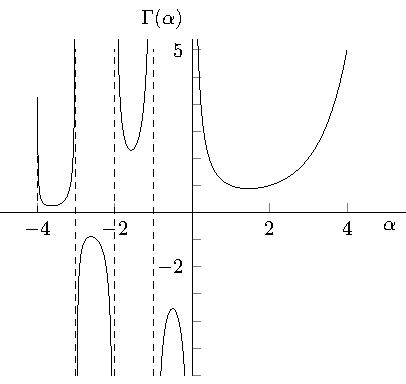
\includegraphics{figOctaveGammaFunction}
\caption{گیما تفاعل}
\label{شکل_ضمیمہ_مفید_گیما_تفاعل}
\end{figure}
%

\اصطلاح{نا مکمل گیما تفاعل}
\begin{align}
P(\alpha,x)=\int_{0}^{x} e^{-t}t^{\alpha-1}\dif t, \quad Q(\alpha,x)=\int_{x}^{\infty} e^{-t}t^{\alpha-1}\dif t \quad \quad (\alpha>0)
\end{align}
%
\begin{align}
\Gamma(\alpha)=P(\alpha,x)+Q(\alpha,x)
\end{align}
\اصطلاح{بیٹا تفاعل}
\begin{align}
B(x,y)=\int_{0}^{1}t^{x-1}(1-t)^{y-1}\dif t\quad \quad (x>0,\, y>0)
\end{align}
بیٹا تفاعل کو گیما تفاعل کی صورت میں بھی پیش کیا جا سکتا ہے۔
\begin{align}
B(x,y)=\frac{\Gamma(x) \Gamma(y)}{\Gamma(x+y)}
\end{align}
\اصطلاح{تفاعل خلل}(شکل \حوالہ{شکل_ضمیمہ_مفید_تفاعل_خلل})
\begin{align}\label{مساوات_ضمیمہ_تفاعل_خلل_الف}
\erf x=\frac{2}{\sqrt{\pi}}\int_{0}^{x} e^{-t^2}\dif t
\end{align}
مساوات \حوالہ{مساوات_ضمیمہ_تفاعل_خلل_الف} کے تفرق \عددی{\erf' x=\tfrac{2}{\sqrt{\pi}}e^{-t^2}} کی مکلارن تسلسل 
\begin{align*}
\erf' x=\frac{2}{\sqrt{\pi}}\left(x-\frac{x^3}{1!3}+\frac{x^5}{2!5}-\frac{x^7}{3!7}+-\cdots \right)
\end{align*}
 کا تکمل لینے سے تفاعل خلل کی تسلسل صورت حاصل ہوتی ہے۔
%
\begin{align}
\erf x=\frac{2}{\sqrt{\pi}}\left(x-\frac{x^3}{1!3}+\frac{x^5}{2!5}-\frac{x^7}{3!7}+-\cdots \right)
\end{align}
\عددی{erf \infty =1} ہے۔ \اصطلاح{مکملہ تفاعل خلل}
\begin{align}
\erfc x=1-\erf x=\frac{2}{\sqrt{\pi}} \int_{x}^{\infty} e^{-t^2}\dif t
\end{align}
%
\begin{figure}
\centering
\begin{tikzpicture}[
    declare function={erf(\x)=%
      (1+(e^(-(\x*\x))*(-265.057+abs(\x)*(-135.065+abs(\x)%
      *(-59.646+(-6.84727-0.777889*abs(\x))*abs(\x)))))%
      /(3.05259+abs(\x))^5)*(\x>0?1:-1);},
    declare function={erf2(\x,\y)=erf(\x)+erf(\y);}
]
\begin{axis}[small,axis lines*=middle,xlabel={$x$},ylabel={$\erf x$},xlabel style={at={(current axis.right of origin)},anchor=north east},ylabel style={rotate=-90},ylabel style={at={(current axis.above origin)},anchor=north east},ymin=-1.2,ymax=1.5,xmin=-2.2,xmax=3,xtick={-2,-1,1,2},xticklabels={{$-2$},{$-1$},{$1$},{$2$}},ytick={-1,1},yticklabels={{$-1$},{$1$}}]
\addplot[domain=-2:2]{erf(\x)};
\end{axis}
\end{tikzpicture}
\caption{تفاعل خلل۔}
\label{شکل_ضمیمہ_مفید_تفاعل_خلل}
\end{figure}
\اصطلاح{فرسنل تکملات} (شکل \حوالہ{شکل_ضمیمہ_مفید_فرسنل_تکملات})
\begin{align}
\FC(x)=\int_{0}^{x} \cos(t^2)\dif t,\quad \FS(x)=\int_{0}^{x}\sin(t^2)\dif t
\end{align}
\عددی{\FC(\infty)=\sqrt{\tfrac{\pi}{8}}} اور \عددی{\FS(\infty)=\sqrt{\tfrac{\pi}{8}}} ہیں۔\اصطلاح{مکملہ تفاعل}\حاشیہب{complementary functions}
\begin{align}
\FAC(x)&=\frac{\pi}{8}-\FC(x)=\int_{x}^{\infty} \cos(t^2)\dif t\\
\FAS(x)&=\frac{\pi}{8}-\FS(x)=\int_{x}^{\infty} \sin(t^2)\dif t
\end{align}
%
\begin{figure}
\centering
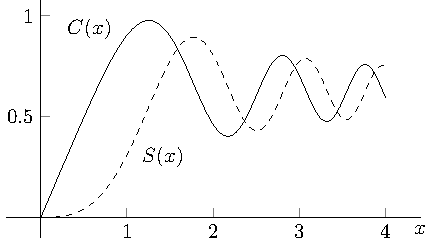
\includegraphics{figFresnelIntegrals}
\caption{فرسنل تکملات}
\label{شکل_ضمیمہ_مفید_فرسنل_تکملات}
\end{figure}
\اصطلاح{تکمل سائن} (شکل \حوالہ{شکل_ضمیمہ_مفید_تکمل_سائن})
\begin{align}
\kSi(x)=\int_{0}^{x}\frac{\sin t}{t} \dif t
\end{align}
\عددی{\kSi{\infty}=\tfrac{\pi}{2}} کے برابر ہے۔تکملہ تفاعل
\begin{align}
\ksi(x)=\frac{\pi}{2}-\kSi(x)=\int_{x}^{\infty} \frac{\sin t}{t}\dif t
\end{align}
\اصطلاح{تکمل کوسائن}
\begin{align}
\ci(x)=\int_{x}^{\infty}\frac{\cos t}{t}\dif t \quad \quad (x>0)
\end{align}
\اصطلاح{تکمل قوت نمائی}
\begin{align}
\Ei(x)=\int_{x}^{\infty} \frac{e^{-t}}{t}\dif t\quad \quad (x>0)
\end{align}
\اصطلاح{تکمل لوگارتھمی}
\begin{align}
\li(x)=\int_{0}^{x}\frac{\dif t}{\ln t}
\end{align}
%
\begin{figure}
\centering
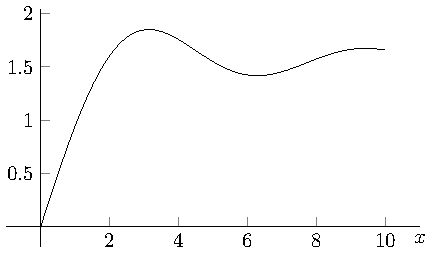
\includegraphics{figSineIntegral}
\caption{تکمل سائن}
\label{شکل_ضمیمہ_مفید_تکمل_سائن}
\end{figure}

%

%\include{./tex/emtEndOfBookTableDivergenceCurlGradientLaplacian}
%\include{./tex/toDoList}
%\include{./tex/emtQuestions}
\backmatter

\cleardoublepage
%\include{./tex/emtDataTables}        %appendices
%\include{./tex/emtLinearAlgebra}
%\include{./tex/emtCoordinatesRelations}
%================


%=================

\renewcommand*{\indexname}{فرہنگ}      %this command has to be placed right here just before printindex command
\cleardoublepage
\addcontentsline{toc}{chapter}{فرہنگ}
%\printindex


\end{urdufont}
\end{document}
